\begin{figure}[htpb]
    \centering
    %% Creator: Matplotlib, PGF backend
%%
%% To include the figure in your LaTeX document, write
%%   \input{<filename>.pgf}
%%
%% Make sure the required packages are loaded in your preamble
%%   \usepackage{pgf}
%%
%% Figures using additional raster images can only be included by \input if
%% they are in the same directory as the main LaTeX file. For loading figures
%% from other directories you can use the `import` package
%%   \usepackage{import}
%% and then include the figures with
%%   \import{<path to file>}{<filename>.pgf}
%%
%% Matplotlib used the following preamble
%%   \usepackage[utf8x]{inputenc}
%%   \usepackage[T1]{fontenc}
%%   \usepackage[]{libertine}\usepackage[libertine]{newtxmath}
%%
\begingroup%
\makeatletter%
\begin{pgfpicture}%
\pgfpathrectangle{\pgfpointorigin}{\pgfqpoint{5.050000in}{3.100000in}}%
\pgfusepath{use as bounding box, clip}%
\begin{pgfscope}%
\pgfsetbuttcap%
\pgfsetmiterjoin%
\definecolor{currentfill}{rgb}{1.000000,1.000000,1.000000}%
\pgfsetfillcolor{currentfill}%
\pgfsetlinewidth{0.000000pt}%
\definecolor{currentstroke}{rgb}{1.000000,1.000000,1.000000}%
\pgfsetstrokecolor{currentstroke}%
\pgfsetdash{}{0pt}%
\pgfpathmoveto{\pgfqpoint{0.000000in}{0.000000in}}%
\pgfpathlineto{\pgfqpoint{5.050000in}{0.000000in}}%
\pgfpathlineto{\pgfqpoint{5.050000in}{3.100000in}}%
\pgfpathlineto{\pgfqpoint{0.000000in}{3.100000in}}%
\pgfpathclose%
\pgfusepath{fill}%
\end{pgfscope}%
\begin{pgfscope}%
\pgfsetbuttcap%
\pgfsetmiterjoin%
\definecolor{currentfill}{rgb}{1.000000,1.000000,1.000000}%
\pgfsetfillcolor{currentfill}%
\pgfsetlinewidth{0.000000pt}%
\definecolor{currentstroke}{rgb}{0.000000,0.000000,0.000000}%
\pgfsetstrokecolor{currentstroke}%
\pgfsetstrokeopacity{0.000000}%
\pgfsetdash{}{0pt}%
\pgfpathmoveto{\pgfqpoint{0.448634in}{0.402556in}}%
\pgfpathlineto{\pgfqpoint{4.799294in}{0.402556in}}%
\pgfpathlineto{\pgfqpoint{4.799294in}{2.891760in}}%
\pgfpathlineto{\pgfqpoint{0.448634in}{2.891760in}}%
\pgfpathclose%
\pgfusepath{fill}%
\end{pgfscope}%
\begin{pgfscope}%
\pgfsetbuttcap%
\pgfsetroundjoin%
\definecolor{currentfill}{rgb}{0.000000,0.000000,0.000000}%
\pgfsetfillcolor{currentfill}%
\pgfsetlinewidth{0.803000pt}%
\definecolor{currentstroke}{rgb}{0.000000,0.000000,0.000000}%
\pgfsetstrokecolor{currentstroke}%
\pgfsetdash{}{0pt}%
\pgfsys@defobject{currentmarker}{\pgfqpoint{0.000000in}{-0.048611in}}{\pgfqpoint{0.000000in}{0.000000in}}{%
\pgfpathmoveto{\pgfqpoint{0.000000in}{0.000000in}}%
\pgfpathlineto{\pgfqpoint{0.000000in}{-0.048611in}}%
\pgfusepath{stroke,fill}%
}%
\begin{pgfscope}%
\pgfsys@transformshift{0.448634in}{0.402556in}%
\pgfsys@useobject{currentmarker}{}%
\end{pgfscope}%
\end{pgfscope}%
\begin{pgfscope}%
\pgftext[x=0.448634in,y=0.305334in,,top]{\rmfamily\fontsize{12.000000}{14.400000}\selectfont \(\displaystyle 0.00\)}%
\end{pgfscope}%
\begin{pgfscope}%
\pgfsetbuttcap%
\pgfsetroundjoin%
\definecolor{currentfill}{rgb}{0.000000,0.000000,0.000000}%
\pgfsetfillcolor{currentfill}%
\pgfsetlinewidth{0.803000pt}%
\definecolor{currentstroke}{rgb}{0.000000,0.000000,0.000000}%
\pgfsetstrokecolor{currentstroke}%
\pgfsetdash{}{0pt}%
\pgfsys@defobject{currentmarker}{\pgfqpoint{0.000000in}{-0.048611in}}{\pgfqpoint{0.000000in}{0.000000in}}{%
\pgfpathmoveto{\pgfqpoint{0.000000in}{0.000000in}}%
\pgfpathlineto{\pgfqpoint{0.000000in}{-0.048611in}}%
\pgfusepath{stroke,fill}%
}%
\begin{pgfscope}%
\pgfsys@transformshift{0.992466in}{0.402556in}%
\pgfsys@useobject{currentmarker}{}%
\end{pgfscope}%
\end{pgfscope}%
\begin{pgfscope}%
\pgftext[x=0.992466in,y=0.305334in,,top]{\rmfamily\fontsize{12.000000}{14.400000}\selectfont \(\displaystyle 0.25\)}%
\end{pgfscope}%
\begin{pgfscope}%
\pgfsetbuttcap%
\pgfsetroundjoin%
\definecolor{currentfill}{rgb}{0.000000,0.000000,0.000000}%
\pgfsetfillcolor{currentfill}%
\pgfsetlinewidth{0.803000pt}%
\definecolor{currentstroke}{rgb}{0.000000,0.000000,0.000000}%
\pgfsetstrokecolor{currentstroke}%
\pgfsetdash{}{0pt}%
\pgfsys@defobject{currentmarker}{\pgfqpoint{0.000000in}{-0.048611in}}{\pgfqpoint{0.000000in}{0.000000in}}{%
\pgfpathmoveto{\pgfqpoint{0.000000in}{0.000000in}}%
\pgfpathlineto{\pgfqpoint{0.000000in}{-0.048611in}}%
\pgfusepath{stroke,fill}%
}%
\begin{pgfscope}%
\pgfsys@transformshift{1.536299in}{0.402556in}%
\pgfsys@useobject{currentmarker}{}%
\end{pgfscope}%
\end{pgfscope}%
\begin{pgfscope}%
\pgftext[x=1.536299in,y=0.305334in,,top]{\rmfamily\fontsize{12.000000}{14.400000}\selectfont \(\displaystyle 0.50\)}%
\end{pgfscope}%
\begin{pgfscope}%
\pgfsetbuttcap%
\pgfsetroundjoin%
\definecolor{currentfill}{rgb}{0.000000,0.000000,0.000000}%
\pgfsetfillcolor{currentfill}%
\pgfsetlinewidth{0.803000pt}%
\definecolor{currentstroke}{rgb}{0.000000,0.000000,0.000000}%
\pgfsetstrokecolor{currentstroke}%
\pgfsetdash{}{0pt}%
\pgfsys@defobject{currentmarker}{\pgfqpoint{0.000000in}{-0.048611in}}{\pgfqpoint{0.000000in}{0.000000in}}{%
\pgfpathmoveto{\pgfqpoint{0.000000in}{0.000000in}}%
\pgfpathlineto{\pgfqpoint{0.000000in}{-0.048611in}}%
\pgfusepath{stroke,fill}%
}%
\begin{pgfscope}%
\pgfsys@transformshift{2.080131in}{0.402556in}%
\pgfsys@useobject{currentmarker}{}%
\end{pgfscope}%
\end{pgfscope}%
\begin{pgfscope}%
\pgftext[x=2.080131in,y=0.305334in,,top]{\rmfamily\fontsize{12.000000}{14.400000}\selectfont \(\displaystyle 0.75\)}%
\end{pgfscope}%
\begin{pgfscope}%
\pgfsetbuttcap%
\pgfsetroundjoin%
\definecolor{currentfill}{rgb}{0.000000,0.000000,0.000000}%
\pgfsetfillcolor{currentfill}%
\pgfsetlinewidth{0.803000pt}%
\definecolor{currentstroke}{rgb}{0.000000,0.000000,0.000000}%
\pgfsetstrokecolor{currentstroke}%
\pgfsetdash{}{0pt}%
\pgfsys@defobject{currentmarker}{\pgfqpoint{0.000000in}{-0.048611in}}{\pgfqpoint{0.000000in}{0.000000in}}{%
\pgfpathmoveto{\pgfqpoint{0.000000in}{0.000000in}}%
\pgfpathlineto{\pgfqpoint{0.000000in}{-0.048611in}}%
\pgfusepath{stroke,fill}%
}%
\begin{pgfscope}%
\pgfsys@transformshift{2.623964in}{0.402556in}%
\pgfsys@useobject{currentmarker}{}%
\end{pgfscope}%
\end{pgfscope}%
\begin{pgfscope}%
\pgftext[x=2.623964in,y=0.305334in,,top]{\rmfamily\fontsize{12.000000}{14.400000}\selectfont \(\displaystyle 1.00\)}%
\end{pgfscope}%
\begin{pgfscope}%
\pgfsetbuttcap%
\pgfsetroundjoin%
\definecolor{currentfill}{rgb}{0.000000,0.000000,0.000000}%
\pgfsetfillcolor{currentfill}%
\pgfsetlinewidth{0.803000pt}%
\definecolor{currentstroke}{rgb}{0.000000,0.000000,0.000000}%
\pgfsetstrokecolor{currentstroke}%
\pgfsetdash{}{0pt}%
\pgfsys@defobject{currentmarker}{\pgfqpoint{0.000000in}{-0.048611in}}{\pgfqpoint{0.000000in}{0.000000in}}{%
\pgfpathmoveto{\pgfqpoint{0.000000in}{0.000000in}}%
\pgfpathlineto{\pgfqpoint{0.000000in}{-0.048611in}}%
\pgfusepath{stroke,fill}%
}%
\begin{pgfscope}%
\pgfsys@transformshift{3.167797in}{0.402556in}%
\pgfsys@useobject{currentmarker}{}%
\end{pgfscope}%
\end{pgfscope}%
\begin{pgfscope}%
\pgftext[x=3.167797in,y=0.305334in,,top]{\rmfamily\fontsize{12.000000}{14.400000}\selectfont \(\displaystyle 1.25\)}%
\end{pgfscope}%
\begin{pgfscope}%
\pgfsetbuttcap%
\pgfsetroundjoin%
\definecolor{currentfill}{rgb}{0.000000,0.000000,0.000000}%
\pgfsetfillcolor{currentfill}%
\pgfsetlinewidth{0.803000pt}%
\definecolor{currentstroke}{rgb}{0.000000,0.000000,0.000000}%
\pgfsetstrokecolor{currentstroke}%
\pgfsetdash{}{0pt}%
\pgfsys@defobject{currentmarker}{\pgfqpoint{0.000000in}{-0.048611in}}{\pgfqpoint{0.000000in}{0.000000in}}{%
\pgfpathmoveto{\pgfqpoint{0.000000in}{0.000000in}}%
\pgfpathlineto{\pgfqpoint{0.000000in}{-0.048611in}}%
\pgfusepath{stroke,fill}%
}%
\begin{pgfscope}%
\pgfsys@transformshift{3.711629in}{0.402556in}%
\pgfsys@useobject{currentmarker}{}%
\end{pgfscope}%
\end{pgfscope}%
\begin{pgfscope}%
\pgftext[x=3.711629in,y=0.305334in,,top]{\rmfamily\fontsize{12.000000}{14.400000}\selectfont \(\displaystyle 1.50\)}%
\end{pgfscope}%
\begin{pgfscope}%
\pgfsetbuttcap%
\pgfsetroundjoin%
\definecolor{currentfill}{rgb}{0.000000,0.000000,0.000000}%
\pgfsetfillcolor{currentfill}%
\pgfsetlinewidth{0.803000pt}%
\definecolor{currentstroke}{rgb}{0.000000,0.000000,0.000000}%
\pgfsetstrokecolor{currentstroke}%
\pgfsetdash{}{0pt}%
\pgfsys@defobject{currentmarker}{\pgfqpoint{0.000000in}{-0.048611in}}{\pgfqpoint{0.000000in}{0.000000in}}{%
\pgfpathmoveto{\pgfqpoint{0.000000in}{0.000000in}}%
\pgfpathlineto{\pgfqpoint{0.000000in}{-0.048611in}}%
\pgfusepath{stroke,fill}%
}%
\begin{pgfscope}%
\pgfsys@transformshift{4.255462in}{0.402556in}%
\pgfsys@useobject{currentmarker}{}%
\end{pgfscope}%
\end{pgfscope}%
\begin{pgfscope}%
\pgftext[x=4.255462in,y=0.305334in,,top]{\rmfamily\fontsize{12.000000}{14.400000}\selectfont \(\displaystyle 1.75\)}%
\end{pgfscope}%
\begin{pgfscope}%
\pgfsetbuttcap%
\pgfsetroundjoin%
\definecolor{currentfill}{rgb}{0.000000,0.000000,0.000000}%
\pgfsetfillcolor{currentfill}%
\pgfsetlinewidth{0.803000pt}%
\definecolor{currentstroke}{rgb}{0.000000,0.000000,0.000000}%
\pgfsetstrokecolor{currentstroke}%
\pgfsetdash{}{0pt}%
\pgfsys@defobject{currentmarker}{\pgfqpoint{0.000000in}{-0.048611in}}{\pgfqpoint{0.000000in}{0.000000in}}{%
\pgfpathmoveto{\pgfqpoint{0.000000in}{0.000000in}}%
\pgfpathlineto{\pgfqpoint{0.000000in}{-0.048611in}}%
\pgfusepath{stroke,fill}%
}%
\begin{pgfscope}%
\pgfsys@transformshift{4.799294in}{0.402556in}%
\pgfsys@useobject{currentmarker}{}%
\end{pgfscope}%
\end{pgfscope}%
\begin{pgfscope}%
\pgftext[x=4.799294in,y=0.305334in,,top]{\rmfamily\fontsize{12.000000}{14.400000}\selectfont \(\displaystyle 2.00\)}%
\end{pgfscope}%
\begin{pgfscope}%
\pgfsetbuttcap%
\pgfsetroundjoin%
\definecolor{currentfill}{rgb}{0.000000,0.000000,0.000000}%
\pgfsetfillcolor{currentfill}%
\pgfsetlinewidth{0.803000pt}%
\definecolor{currentstroke}{rgb}{0.000000,0.000000,0.000000}%
\pgfsetstrokecolor{currentstroke}%
\pgfsetdash{}{0pt}%
\pgfsys@defobject{currentmarker}{\pgfqpoint{-0.048611in}{0.000000in}}{\pgfqpoint{0.000000in}{0.000000in}}{%
\pgfpathmoveto{\pgfqpoint{0.000000in}{0.000000in}}%
\pgfpathlineto{\pgfqpoint{-0.048611in}{0.000000in}}%
\pgfusepath{stroke,fill}%
}%
\begin{pgfscope}%
\pgfsys@transformshift{0.448634in}{0.402556in}%
\pgfsys@useobject{currentmarker}{}%
\end{pgfscope}%
\end{pgfscope}%
\begin{pgfscope}%
\pgftext[x=0.149245in,y=0.345015in,left,base]{\rmfamily\fontsize{12.000000}{14.400000}\selectfont \(\displaystyle 0.0\)}%
\end{pgfscope}%
\begin{pgfscope}%
\pgfsetbuttcap%
\pgfsetroundjoin%
\definecolor{currentfill}{rgb}{0.000000,0.000000,0.000000}%
\pgfsetfillcolor{currentfill}%
\pgfsetlinewidth{0.803000pt}%
\definecolor{currentstroke}{rgb}{0.000000,0.000000,0.000000}%
\pgfsetstrokecolor{currentstroke}%
\pgfsetdash{}{0pt}%
\pgfsys@defobject{currentmarker}{\pgfqpoint{-0.048611in}{0.000000in}}{\pgfqpoint{0.000000in}{0.000000in}}{%
\pgfpathmoveto{\pgfqpoint{0.000000in}{0.000000in}}%
\pgfpathlineto{\pgfqpoint{-0.048611in}{0.000000in}}%
\pgfusepath{stroke,fill}%
}%
\begin{pgfscope}%
\pgfsys@transformshift{0.448634in}{0.900397in}%
\pgfsys@useobject{currentmarker}{}%
\end{pgfscope}%
\end{pgfscope}%
\begin{pgfscope}%
\pgftext[x=0.149245in,y=0.842855in,left,base]{\rmfamily\fontsize{12.000000}{14.400000}\selectfont \(\displaystyle 0.2\)}%
\end{pgfscope}%
\begin{pgfscope}%
\pgfsetbuttcap%
\pgfsetroundjoin%
\definecolor{currentfill}{rgb}{0.000000,0.000000,0.000000}%
\pgfsetfillcolor{currentfill}%
\pgfsetlinewidth{0.803000pt}%
\definecolor{currentstroke}{rgb}{0.000000,0.000000,0.000000}%
\pgfsetstrokecolor{currentstroke}%
\pgfsetdash{}{0pt}%
\pgfsys@defobject{currentmarker}{\pgfqpoint{-0.048611in}{0.000000in}}{\pgfqpoint{0.000000in}{0.000000in}}{%
\pgfpathmoveto{\pgfqpoint{0.000000in}{0.000000in}}%
\pgfpathlineto{\pgfqpoint{-0.048611in}{0.000000in}}%
\pgfusepath{stroke,fill}%
}%
\begin{pgfscope}%
\pgfsys@transformshift{0.448634in}{1.398238in}%
\pgfsys@useobject{currentmarker}{}%
\end{pgfscope}%
\end{pgfscope}%
\begin{pgfscope}%
\pgftext[x=0.149245in,y=1.340696in,left,base]{\rmfamily\fontsize{12.000000}{14.400000}\selectfont \(\displaystyle 0.4\)}%
\end{pgfscope}%
\begin{pgfscope}%
\pgfsetbuttcap%
\pgfsetroundjoin%
\definecolor{currentfill}{rgb}{0.000000,0.000000,0.000000}%
\pgfsetfillcolor{currentfill}%
\pgfsetlinewidth{0.803000pt}%
\definecolor{currentstroke}{rgb}{0.000000,0.000000,0.000000}%
\pgfsetstrokecolor{currentstroke}%
\pgfsetdash{}{0pt}%
\pgfsys@defobject{currentmarker}{\pgfqpoint{-0.048611in}{0.000000in}}{\pgfqpoint{0.000000in}{0.000000in}}{%
\pgfpathmoveto{\pgfqpoint{0.000000in}{0.000000in}}%
\pgfpathlineto{\pgfqpoint{-0.048611in}{0.000000in}}%
\pgfusepath{stroke,fill}%
}%
\begin{pgfscope}%
\pgfsys@transformshift{0.448634in}{1.896079in}%
\pgfsys@useobject{currentmarker}{}%
\end{pgfscope}%
\end{pgfscope}%
\begin{pgfscope}%
\pgftext[x=0.149245in,y=1.838537in,left,base]{\rmfamily\fontsize{12.000000}{14.400000}\selectfont \(\displaystyle 0.6\)}%
\end{pgfscope}%
\begin{pgfscope}%
\pgfsetbuttcap%
\pgfsetroundjoin%
\definecolor{currentfill}{rgb}{0.000000,0.000000,0.000000}%
\pgfsetfillcolor{currentfill}%
\pgfsetlinewidth{0.803000pt}%
\definecolor{currentstroke}{rgb}{0.000000,0.000000,0.000000}%
\pgfsetstrokecolor{currentstroke}%
\pgfsetdash{}{0pt}%
\pgfsys@defobject{currentmarker}{\pgfqpoint{-0.048611in}{0.000000in}}{\pgfqpoint{0.000000in}{0.000000in}}{%
\pgfpathmoveto{\pgfqpoint{0.000000in}{0.000000in}}%
\pgfpathlineto{\pgfqpoint{-0.048611in}{0.000000in}}%
\pgfusepath{stroke,fill}%
}%
\begin{pgfscope}%
\pgfsys@transformshift{0.448634in}{2.393919in}%
\pgfsys@useobject{currentmarker}{}%
\end{pgfscope}%
\end{pgfscope}%
\begin{pgfscope}%
\pgftext[x=0.149245in,y=2.336378in,left,base]{\rmfamily\fontsize{12.000000}{14.400000}\selectfont \(\displaystyle 0.8\)}%
\end{pgfscope}%
\begin{pgfscope}%
\pgfsetbuttcap%
\pgfsetroundjoin%
\definecolor{currentfill}{rgb}{0.000000,0.000000,0.000000}%
\pgfsetfillcolor{currentfill}%
\pgfsetlinewidth{0.803000pt}%
\definecolor{currentstroke}{rgb}{0.000000,0.000000,0.000000}%
\pgfsetstrokecolor{currentstroke}%
\pgfsetdash{}{0pt}%
\pgfsys@defobject{currentmarker}{\pgfqpoint{-0.048611in}{0.000000in}}{\pgfqpoint{0.000000in}{0.000000in}}{%
\pgfpathmoveto{\pgfqpoint{0.000000in}{0.000000in}}%
\pgfpathlineto{\pgfqpoint{-0.048611in}{0.000000in}}%
\pgfusepath{stroke,fill}%
}%
\begin{pgfscope}%
\pgfsys@transformshift{0.448634in}{2.891760in}%
\pgfsys@useobject{currentmarker}{}%
\end{pgfscope}%
\end{pgfscope}%
\begin{pgfscope}%
\pgftext[x=0.149245in,y=2.834219in,left,base]{\rmfamily\fontsize{12.000000}{14.400000}\selectfont \(\displaystyle 1.0\)}%
\end{pgfscope}%
\begin{pgfscope}%
\pgfpathrectangle{\pgfqpoint{0.448634in}{0.402556in}}{\pgfqpoint{4.350661in}{2.489204in}} %
\pgfusepath{clip}%
\pgfsetrectcap%
\pgfsetroundjoin%
\pgfsetlinewidth{1.003750pt}%
\definecolor{currentstroke}{rgb}{0.121569,0.466667,0.705882}%
\pgfsetstrokecolor{currentstroke}%
\pgfsetdash{}{0pt}%
\pgfpathmoveto{\pgfqpoint{0.448634in}{2.896245in}}%
\pgfpathlineto{\pgfqpoint{0.448593in}{0.407043in}}%
\pgfpathlineto{\pgfqpoint{0.448593in}{0.407043in}}%
\pgfusepath{stroke}%
\end{pgfscope}%
\begin{pgfscope}%
\pgfpathrectangle{\pgfqpoint{0.448634in}{0.402556in}}{\pgfqpoint{4.350661in}{2.489204in}} %
\pgfusepath{clip}%
\pgfsetrectcap%
\pgfsetroundjoin%
\pgfsetlinewidth{1.003750pt}%
\definecolor{currentstroke}{rgb}{0.121569,0.466667,0.705882}%
\pgfsetstrokecolor{currentstroke}%
\pgfsetdash{}{0pt}%
\pgfpathmoveto{\pgfqpoint{0.576853in}{1.760817in}}%
\pgfpathlineto{\pgfqpoint{0.569394in}{1.840010in}}%
\pgfpathlineto{\pgfqpoint{0.563209in}{1.929338in}}%
\pgfpathlineto{\pgfqpoint{0.558592in}{2.028764in}}%
\pgfpathlineto{\pgfqpoint{0.555985in}{2.133265in}}%
\pgfpathlineto{\pgfqpoint{0.555566in}{2.237808in}}%
\pgfpathlineto{\pgfqpoint{0.557371in}{2.337352in}}%
\pgfpathlineto{\pgfqpoint{0.561096in}{2.424366in}}%
\pgfpathlineto{\pgfqpoint{0.566403in}{2.498791in}}%
\pgfpathlineto{\pgfqpoint{0.572909in}{2.560570in}}%
\pgfpathlineto{\pgfqpoint{0.580458in}{2.612119in}}%
\pgfpathlineto{\pgfqpoint{0.589086in}{2.655816in}}%
\pgfpathlineto{\pgfqpoint{0.598406in}{2.691589in}}%
\pgfpathlineto{\pgfqpoint{0.608613in}{2.721757in}}%
\pgfpathlineto{\pgfqpoint{0.619241in}{2.746278in}}%
\pgfpathlineto{\pgfqpoint{0.630817in}{2.767339in}}%
\pgfpathlineto{\pgfqpoint{0.642975in}{2.784884in}}%
\pgfpathlineto{\pgfqpoint{0.656813in}{2.800712in}}%
\pgfpathlineto{\pgfqpoint{0.672197in}{2.814549in}}%
\pgfpathlineto{\pgfqpoint{0.688853in}{2.826301in}}%
\pgfpathlineto{\pgfqpoint{0.706461in}{2.836076in}}%
\pgfpathlineto{\pgfqpoint{0.726804in}{2.844875in}}%
\pgfpathlineto{\pgfqpoint{0.751866in}{2.853203in}}%
\pgfpathlineto{\pgfqpoint{0.781631in}{2.860547in}}%
\pgfpathlineto{\pgfqpoint{0.818168in}{2.867054in}}%
\pgfpathlineto{\pgfqpoint{0.863581in}{2.872685in}}%
\pgfpathlineto{\pgfqpoint{0.922161in}{2.877518in}}%
\pgfpathlineto{\pgfqpoint{1.000391in}{2.881567in}}%
\pgfpathlineto{\pgfqpoint{1.111294in}{2.884881in}}%
\pgfpathlineto{\pgfqpoint{1.274428in}{2.887367in}}%
\pgfpathlineto{\pgfqpoint{1.552865in}{2.889263in}}%
\pgfpathlineto{\pgfqpoint{2.107573in}{2.890457in}}%
\pgfpathlineto{\pgfqpoint{3.343161in}{2.890573in}}%
\pgfpathlineto{\pgfqpoint{4.043615in}{2.888941in}}%
\pgfpathlineto{\pgfqpoint{4.289417in}{2.886404in}}%
\pgfpathlineto{\pgfqpoint{4.413375in}{2.883093in}}%
\pgfpathlineto{\pgfqpoint{4.489424in}{2.878997in}}%
\pgfpathlineto{\pgfqpoint{4.541451in}{2.874081in}}%
\pgfpathlineto{\pgfqpoint{4.578100in}{2.868470in}}%
\pgfpathlineto{\pgfqpoint{4.605818in}{2.862092in}}%
\pgfpathlineto{\pgfqpoint{4.626725in}{2.855245in}}%
\pgfpathlineto{\pgfqpoint{4.644925in}{2.847018in}}%
\pgfpathlineto{\pgfqpoint{4.660241in}{2.837590in}}%
\pgfpathlineto{\pgfqpoint{4.672623in}{2.827468in}}%
\pgfpathlineto{\pgfqpoint{4.683751in}{2.815592in}}%
\pgfpathlineto{\pgfqpoint{4.693406in}{2.802135in}}%
\pgfpathlineto{\pgfqpoint{4.702740in}{2.785343in}}%
\pgfpathlineto{\pgfqpoint{4.711277in}{2.765194in}}%
\pgfpathlineto{\pgfqpoint{4.719482in}{2.739484in}}%
\pgfpathlineto{\pgfqpoint{4.726293in}{2.710657in}}%
\pgfpathlineto{\pgfqpoint{4.733259in}{2.671643in}}%
\pgfpathlineto{\pgfqpoint{4.739604in}{2.622396in}}%
\pgfpathlineto{\pgfqpoint{4.745236in}{2.560504in}}%
\pgfpathlineto{\pgfqpoint{4.750164in}{2.481052in}}%
\pgfpathlineto{\pgfqpoint{4.754367in}{2.376618in}}%
\pgfpathlineto{\pgfqpoint{4.757443in}{2.242249in}}%
\pgfpathlineto{\pgfqpoint{4.758977in}{2.075483in}}%
\pgfpathlineto{\pgfqpoint{4.758447in}{1.888795in}}%
\pgfpathlineto{\pgfqpoint{4.755756in}{1.707111in}}%
\pgfpathlineto{\pgfqpoint{4.750925in}{1.532957in}}%
\pgfpathlineto{\pgfqpoint{4.744785in}{1.398726in}}%
\pgfpathlineto{\pgfqpoint{4.737575in}{1.289516in}}%
\pgfpathlineto{\pgfqpoint{4.728714in}{1.190470in}}%
\pgfpathlineto{\pgfqpoint{4.719652in}{1.116521in}}%
\pgfpathlineto{\pgfqpoint{4.710036in}{1.055276in}}%
\pgfpathlineto{\pgfqpoint{4.699503in}{1.001861in}}%
\pgfpathlineto{\pgfqpoint{4.689040in}{0.958690in}}%
\pgfpathlineto{\pgfqpoint{4.677219in}{0.918600in}}%
\pgfpathlineto{\pgfqpoint{4.664034in}{0.881749in}}%
\pgfpathlineto{\pgfqpoint{4.650584in}{0.850492in}}%
\pgfpathlineto{\pgfqpoint{4.636303in}{0.822570in}}%
\pgfpathlineto{\pgfqpoint{4.620207in}{0.795974in}}%
\pgfpathlineto{\pgfqpoint{4.603640in}{0.772901in}}%
\pgfpathlineto{\pgfqpoint{4.585488in}{0.751446in}}%
\pgfpathlineto{\pgfqpoint{4.565874in}{0.731749in}}%
\pgfpathlineto{\pgfqpoint{4.544964in}{0.713879in}}%
\pgfpathlineto{\pgfqpoint{4.522958in}{0.697824in}}%
\pgfpathlineto{\pgfqpoint{4.496157in}{0.681290in}}%
\pgfpathlineto{\pgfqpoint{4.470397in}{0.667953in}}%
\pgfpathlineto{\pgfqpoint{4.439961in}{0.654509in}}%
\pgfpathlineto{\pgfqpoint{4.406841in}{0.642281in}}%
\pgfpathlineto{\pgfqpoint{4.369009in}{0.630748in}}%
\pgfpathlineto{\pgfqpoint{4.326489in}{0.620226in}}%
\pgfpathlineto{\pgfqpoint{4.279327in}{0.610949in}}%
\pgfpathlineto{\pgfqpoint{4.227576in}{0.603085in}}%
\pgfpathlineto{\pgfqpoint{4.173450in}{0.597063in}}%
\pgfpathlineto{\pgfqpoint{4.110511in}{0.592203in}}%
\pgfpathlineto{\pgfqpoint{4.047471in}{0.589537in}}%
\pgfpathlineto{\pgfqpoint{3.977867in}{0.588624in}}%
\pgfpathlineto{\pgfqpoint{3.906093in}{0.589934in}}%
\pgfpathlineto{\pgfqpoint{3.834377in}{0.593496in}}%
\pgfpathlineto{\pgfqpoint{3.767120in}{0.599067in}}%
\pgfpathlineto{\pgfqpoint{3.704364in}{0.606392in}}%
\pgfpathlineto{\pgfqpoint{3.678516in}{0.610510in}}%
\pgfpathlineto{\pgfqpoint{3.620438in}{0.620500in}}%
\pgfpathlineto{\pgfqpoint{3.586319in}{0.628207in}}%
\pgfpathlineto{\pgfqpoint{3.495240in}{0.652428in}}%
\pgfpathlineto{\pgfqpoint{3.451528in}{0.667583in}}%
\pgfpathlineto{\pgfqpoint{3.408538in}{0.685220in}}%
\pgfpathlineto{\pgfqpoint{3.374594in}{0.702001in}}%
\pgfpathlineto{\pgfqpoint{3.345407in}{0.718682in}}%
\pgfpathlineto{\pgfqpoint{3.315236in}{0.738520in}}%
\pgfpathlineto{\pgfqpoint{3.288127in}{0.759290in}}%
\pgfpathlineto{\pgfqpoint{3.264004in}{0.780551in}}%
\pgfpathlineto{\pgfqpoint{3.241208in}{0.803648in}}%
\pgfpathlineto{\pgfqpoint{3.219894in}{0.828530in}}%
\pgfpathlineto{\pgfqpoint{3.200189in}{0.855091in}}%
\pgfpathlineto{\pgfqpoint{3.182177in}{0.883182in}}%
\pgfpathlineto{\pgfqpoint{3.165906in}{0.912633in}}%
\pgfpathlineto{\pgfqpoint{3.150351in}{0.945448in}}%
\pgfpathlineto{\pgfqpoint{3.136682in}{0.979345in}}%
\pgfpathlineto{\pgfqpoint{3.124073in}{1.016460in}}%
\pgfpathlineto{\pgfqpoint{3.112834in}{1.056769in}}%
\pgfpathlineto{\pgfqpoint{3.103046in}{1.100146in}}%
\pgfpathlineto{\pgfqpoint{3.095343in}{1.144071in}}%
\pgfpathlineto{\pgfqpoint{3.089208in}{1.190837in}}%
\pgfpathlineto{\pgfqpoint{3.084595in}{1.242838in}}%
\pgfpathlineto{\pgfqpoint{3.082137in}{1.295031in}}%
\pgfpathlineto{\pgfqpoint{3.081687in}{1.349787in}}%
\pgfpathlineto{\pgfqpoint{3.083451in}{1.406998in}}%
\pgfpathlineto{\pgfqpoint{3.087181in}{1.461589in}}%
\pgfpathlineto{\pgfqpoint{3.093485in}{1.520888in}}%
\pgfpathlineto{\pgfqpoint{3.101823in}{1.577334in}}%
\pgfpathlineto{\pgfqpoint{3.111930in}{1.630856in}}%
\pgfpathlineto{\pgfqpoint{3.124690in}{1.686208in}}%
\pgfpathlineto{\pgfqpoint{3.139178in}{1.738395in}}%
\pgfpathlineto{\pgfqpoint{3.155145in}{1.787366in}}%
\pgfpathlineto{\pgfqpoint{3.172353in}{1.833085in}}%
\pgfpathlineto{\pgfqpoint{3.191618in}{1.877716in}}%
\pgfpathlineto{\pgfqpoint{3.214026in}{1.923261in}}%
\pgfpathlineto{\pgfqpoint{3.236214in}{1.963157in}}%
\pgfpathlineto{\pgfqpoint{3.260178in}{2.001684in}}%
\pgfpathlineto{\pgfqpoint{3.285814in}{2.038776in}}%
\pgfpathlineto{\pgfqpoint{3.314415in}{2.076285in}}%
\pgfpathlineto{\pgfqpoint{3.348944in}{2.117711in}}%
\pgfpathlineto{\pgfqpoint{3.417133in}{2.198022in}}%
\pgfpathlineto{\pgfqpoint{3.426053in}{2.212128in}}%
\pgfpathlineto{\pgfqpoint{3.430798in}{2.223297in}}%
\pgfpathlineto{\pgfqpoint{3.432034in}{2.230603in}}%
\pgfpathlineto{\pgfqpoint{3.430773in}{2.237856in}}%
\pgfpathlineto{\pgfqpoint{3.426621in}{2.243526in}}%
\pgfpathlineto{\pgfqpoint{3.420908in}{2.247084in}}%
\pgfpathlineto{\pgfqpoint{3.412501in}{2.249583in}}%
\pgfpathlineto{\pgfqpoint{3.399499in}{2.250689in}}%
\pgfpathlineto{\pgfqpoint{3.384305in}{2.249671in}}%
\pgfpathlineto{\pgfqpoint{3.364985in}{2.246098in}}%
\pgfpathlineto{\pgfqpoint{3.341804in}{2.239342in}}%
\pgfpathlineto{\pgfqpoint{3.317109in}{2.229682in}}%
\pgfpathlineto{\pgfqpoint{3.291104in}{2.216986in}}%
\pgfpathlineto{\pgfqpoint{3.265928in}{2.202261in}}%
\pgfpathlineto{\pgfqpoint{3.239805in}{2.184361in}}%
\pgfpathlineto{\pgfqpoint{3.214775in}{2.164519in}}%
\pgfpathlineto{\pgfqpoint{3.190900in}{2.142893in}}%
\pgfpathlineto{\pgfqpoint{3.166657in}{2.117912in}}%
\pgfpathlineto{\pgfqpoint{3.143835in}{2.091233in}}%
\pgfpathlineto{\pgfqpoint{3.121079in}{2.061107in}}%
\pgfpathlineto{\pgfqpoint{3.099952in}{2.029463in}}%
\pgfpathlineto{\pgfqpoint{3.079251in}{1.994406in}}%
\pgfpathlineto{\pgfqpoint{3.059218in}{1.955915in}}%
\pgfpathlineto{\pgfqpoint{3.040058in}{1.914015in}}%
\pgfpathlineto{\pgfqpoint{3.022809in}{1.871041in}}%
\pgfpathlineto{\pgfqpoint{3.005790in}{1.822536in}}%
\pgfpathlineto{\pgfqpoint{2.990067in}{1.770819in}}%
\pgfpathlineto{\pgfqpoint{2.975708in}{1.715979in}}%
\pgfpathlineto{\pgfqpoint{2.962284in}{1.655680in}}%
\pgfpathlineto{\pgfqpoint{2.950496in}{1.592386in}}%
\pgfpathlineto{\pgfqpoint{2.940383in}{1.526185in}}%
\pgfpathlineto{\pgfqpoint{2.931745in}{1.454681in}}%
\pgfpathlineto{\pgfqpoint{2.925082in}{1.380399in}}%
\pgfpathlineto{\pgfqpoint{2.920647in}{1.305899in}}%
\pgfpathlineto{\pgfqpoint{2.918444in}{1.231270in}}%
\pgfpathlineto{\pgfqpoint{2.918545in}{1.159087in}}%
\pgfpathlineto{\pgfqpoint{2.920787in}{1.091931in}}%
\pgfpathlineto{\pgfqpoint{2.925177in}{1.027412in}}%
\pgfpathlineto{\pgfqpoint{2.931192in}{0.970580in}}%
\pgfpathlineto{\pgfqpoint{2.938760in}{0.919034in}}%
\pgfpathlineto{\pgfqpoint{2.947651in}{0.872852in}}%
\pgfpathlineto{\pgfqpoint{2.958213in}{0.829714in}}%
\pgfpathlineto{\pgfqpoint{2.969670in}{0.792114in}}%
\pgfpathlineto{\pgfqpoint{2.982463in}{0.757773in}}%
\pgfpathlineto{\pgfqpoint{2.996425in}{0.726812in}}%
\pgfpathlineto{\pgfqpoint{3.011299in}{0.699300in}}%
\pgfpathlineto{\pgfqpoint{3.026739in}{0.675225in}}%
\pgfpathlineto{\pgfqpoint{3.043828in}{0.652656in}}%
\pgfpathlineto{\pgfqpoint{3.062495in}{0.631788in}}%
\pgfpathlineto{\pgfqpoint{3.082602in}{0.612753in}}%
\pgfpathlineto{\pgfqpoint{3.103961in}{0.595592in}}%
\pgfpathlineto{\pgfqpoint{3.128268in}{0.579069in}}%
\pgfpathlineto{\pgfqpoint{3.153537in}{0.564554in}}%
\pgfpathlineto{\pgfqpoint{3.181571in}{0.550952in}}%
\pgfpathlineto{\pgfqpoint{3.214371in}{0.537647in}}%
\pgfpathlineto{\pgfqpoint{3.249846in}{0.525712in}}%
\pgfpathlineto{\pgfqpoint{3.290011in}{0.514571in}}%
\pgfpathlineto{\pgfqpoint{3.334820in}{0.504423in}}%
\pgfpathlineto{\pgfqpoint{3.386372in}{0.494999in}}%
\pgfpathlineto{\pgfqpoint{3.446798in}{0.486257in}}%
\pgfpathlineto{\pgfqpoint{3.518243in}{0.478282in}}%
\pgfpathlineto{\pgfqpoint{3.600685in}{0.471409in}}%
\pgfpathlineto{\pgfqpoint{3.696268in}{0.465713in}}%
\pgfpathlineto{\pgfqpoint{3.807144in}{0.461369in}}%
\pgfpathlineto{\pgfqpoint{3.933291in}{0.458719in}}%
\pgfpathlineto{\pgfqpoint{4.063808in}{0.458211in}}%
\pgfpathlineto{\pgfqpoint{4.187792in}{0.459914in}}%
\pgfpathlineto{\pgfqpoint{4.294335in}{0.463521in}}%
\pgfpathlineto{\pgfqpoint{4.381234in}{0.468574in}}%
\pgfpathlineto{\pgfqpoint{4.450636in}{0.474701in}}%
\pgfpathlineto{\pgfqpoint{4.506850in}{0.481799in}}%
\pgfpathlineto{\pgfqpoint{4.552009in}{0.489658in}}%
\pgfpathlineto{\pgfqpoint{4.588239in}{0.498115in}}%
\pgfpathlineto{\pgfqpoint{4.617656in}{0.507110in}}%
\pgfpathlineto{\pgfqpoint{4.642328in}{0.516843in}}%
\pgfpathlineto{\pgfqpoint{4.664194in}{0.527940in}}%
\pgfpathlineto{\pgfqpoint{4.681238in}{0.538945in}}%
\pgfpathlineto{\pgfqpoint{4.697164in}{0.551953in}}%
\pgfpathlineto{\pgfqpoint{4.710076in}{0.565289in}}%
\pgfpathlineto{\pgfqpoint{4.721578in}{0.580218in}}%
\pgfpathlineto{\pgfqpoint{4.731557in}{0.596521in}}%
\pgfpathlineto{\pgfqpoint{4.741000in}{0.616134in}}%
\pgfpathlineto{\pgfqpoint{4.749521in}{0.639027in}}%
\pgfpathlineto{\pgfqpoint{4.757522in}{0.667450in}}%
\pgfpathlineto{\pgfqpoint{4.764572in}{0.701345in}}%
\pgfpathlineto{\pgfqpoint{4.770840in}{0.743043in}}%
\pgfpathlineto{\pgfqpoint{4.776327in}{0.794934in}}%
\pgfpathlineto{\pgfqpoint{4.781278in}{0.864398in}}%
\pgfpathlineto{\pgfqpoint{4.785468in}{0.956371in}}%
\pgfpathlineto{\pgfqpoint{4.789000in}{1.085745in}}%
\pgfpathlineto{\pgfqpoint{4.791852in}{1.277385in}}%
\pgfpathlineto{\pgfqpoint{4.793959in}{1.581057in}}%
\pgfpathlineto{\pgfqpoint{4.794962in}{2.071429in}}%
\pgfpathlineto{\pgfqpoint{4.793967in}{2.559311in}}%
\pgfpathlineto{\pgfqpoint{4.791733in}{2.745981in}}%
\pgfpathlineto{\pgfqpoint{4.788955in}{2.818091in}}%
\pgfpathlineto{\pgfqpoint{4.785731in}{2.850227in}}%
\pgfpathlineto{\pgfqpoint{4.781879in}{2.867057in}}%
\pgfpathlineto{\pgfqpoint{4.777744in}{2.875780in}}%
\pgfpathlineto{\pgfqpoint{4.773097in}{2.880982in}}%
\pgfpathlineto{\pgfqpoint{4.767363in}{2.884504in}}%
\pgfpathlineto{\pgfqpoint{4.756853in}{2.887622in}}%
\pgfpathlineto{\pgfqpoint{4.739548in}{2.889639in}}%
\pgfpathlineto{\pgfqpoint{4.704762in}{2.890882in}}%
\pgfpathlineto{\pgfqpoint{4.602524in}{2.891538in}}%
\pgfpathlineto{\pgfqpoint{3.952100in}{2.891742in}}%
\pgfpathlineto{\pgfqpoint{0.617321in}{2.890753in}}%
\pgfpathlineto{\pgfqpoint{0.549910in}{2.888858in}}%
\pgfpathlineto{\pgfqpoint{0.521735in}{2.886179in}}%
\pgfpathlineto{\pgfqpoint{0.504666in}{2.882389in}}%
\pgfpathlineto{\pgfqpoint{0.494501in}{2.878011in}}%
\pgfpathlineto{\pgfqpoint{0.487180in}{2.872667in}}%
\pgfpathlineto{\pgfqpoint{0.481152in}{2.865519in}}%
\pgfpathlineto{\pgfqpoint{0.475664in}{2.854804in}}%
\pgfpathlineto{\pgfqpoint{0.471318in}{2.840737in}}%
\pgfpathlineto{\pgfqpoint{0.467301in}{2.818823in}}%
\pgfpathlineto{\pgfqpoint{0.463927in}{2.786700in}}%
\pgfpathlineto{\pgfqpoint{0.460918in}{2.734544in}}%
\pgfpathlineto{\pgfqpoint{0.458363in}{2.647473in}}%
\pgfpathlineto{\pgfqpoint{0.456575in}{2.523031in}}%
\pgfpathlineto{\pgfqpoint{0.456575in}{2.523031in}}%
\pgfusepath{stroke}%
\end{pgfscope}%
\begin{pgfscope}%
\pgfpathrectangle{\pgfqpoint{0.448634in}{0.402556in}}{\pgfqpoint{4.350661in}{2.489204in}} %
\pgfusepath{clip}%
\pgfsetrectcap%
\pgfsetroundjoin%
\pgfsetlinewidth{1.003750pt}%
\definecolor{currentstroke}{rgb}{0.121569,0.466667,0.705882}%
\pgfsetstrokecolor{currentstroke}%
\pgfsetdash{}{0pt}%
\pgfpathmoveto{\pgfqpoint{4.798840in}{2.852369in}}%
\pgfpathlineto{\pgfqpoint{4.797564in}{2.889610in}}%
\pgfpathlineto{\pgfqpoint{4.796215in}{2.891483in}}%
\pgfpathlineto{\pgfqpoint{4.787551in}{2.891760in}}%
\pgfpathlineto{\pgfqpoint{0.452128in}{2.891659in}}%
\pgfpathlineto{\pgfqpoint{0.450530in}{2.890082in}}%
\pgfpathlineto{\pgfqpoint{0.449454in}{2.882763in}}%
\pgfpathlineto{\pgfqpoint{0.448970in}{2.845432in}}%
\pgfpathlineto{\pgfqpoint{0.448743in}{2.494454in}}%
\pgfpathlineto{\pgfqpoint{0.449624in}{0.615107in}}%
\pgfpathlineto{\pgfqpoint{0.451433in}{0.510586in}}%
\pgfpathlineto{\pgfqpoint{0.453993in}{0.473374in}}%
\pgfpathlineto{\pgfqpoint{0.457406in}{0.453868in}}%
\pgfpathlineto{\pgfqpoint{0.461540in}{0.442384in}}%
\pgfpathlineto{\pgfqpoint{0.466739in}{0.434437in}}%
\pgfpathlineto{\pgfqpoint{0.473595in}{0.428350in}}%
\pgfpathlineto{\pgfqpoint{0.483492in}{0.423244in}}%
\pgfpathlineto{\pgfqpoint{0.491854in}{0.420501in}}%
\pgfpathlineto{\pgfqpoint{0.491854in}{0.420501in}}%
\pgfusepath{stroke}%
\end{pgfscope}%
\begin{pgfscope}%
\pgfpathrectangle{\pgfqpoint{0.448634in}{0.402556in}}{\pgfqpoint{4.350661in}{2.489204in}} %
\pgfusepath{clip}%
\pgfsetrectcap%
\pgfsetroundjoin%
\pgfsetlinewidth{1.003750pt}%
\definecolor{currentstroke}{rgb}{0.121569,0.466667,0.705882}%
\pgfsetstrokecolor{currentstroke}%
\pgfsetdash{}{0pt}%
\pgfpathmoveto{\pgfqpoint{0.456424in}{1.370137in}}%
\pgfpathlineto{\pgfqpoint{0.459610in}{1.118755in}}%
\pgfpathlineto{\pgfqpoint{0.463695in}{0.962007in}}%
\pgfpathlineto{\pgfqpoint{0.468519in}{0.857610in}}%
\pgfpathlineto{\pgfqpoint{0.474082in}{0.783210in}}%
\pgfpathlineto{\pgfqpoint{0.480226in}{0.728906in}}%
\pgfpathlineto{\pgfqpoint{0.486970in}{0.687306in}}%
\pgfpathlineto{\pgfqpoint{0.494537in}{0.653558in}}%
\pgfpathlineto{\pgfqpoint{0.503107in}{0.625355in}}%
\pgfpathlineto{\pgfqpoint{0.512193in}{0.602750in}}%
\pgfpathlineto{\pgfqpoint{0.522200in}{0.583508in}}%
\pgfpathlineto{\pgfqpoint{0.534108in}{0.565743in}}%
\pgfpathlineto{\pgfqpoint{0.546263in}{0.551507in}}%
\pgfpathlineto{\pgfqpoint{0.559728in}{0.538907in}}%
\pgfpathlineto{\pgfqpoint{0.576129in}{0.526693in}}%
\pgfpathlineto{\pgfqpoint{0.595483in}{0.515351in}}%
\pgfpathlineto{\pgfqpoint{0.617681in}{0.505147in}}%
\pgfpathlineto{\pgfqpoint{0.642568in}{0.496153in}}%
\pgfpathlineto{\pgfqpoint{0.672126in}{0.487778in}}%
\pgfpathlineto{\pgfqpoint{0.708443in}{0.479824in}}%
\pgfpathlineto{\pgfqpoint{0.753649in}{0.472325in}}%
\pgfpathlineto{\pgfqpoint{0.807717in}{0.465660in}}%
\pgfpathlineto{\pgfqpoint{0.877116in}{0.459475in}}%
\pgfpathlineto{\pgfqpoint{0.961828in}{0.454230in}}%
\pgfpathlineto{\pgfqpoint{1.068351in}{0.449916in}}%
\pgfpathlineto{\pgfqpoint{1.201018in}{0.446839in}}%
\pgfpathlineto{\pgfqpoint{1.357637in}{0.445481in}}%
\pgfpathlineto{\pgfqpoint{1.525135in}{0.446232in}}%
\pgfpathlineto{\pgfqpoint{1.686088in}{0.449142in}}%
\pgfpathlineto{\pgfqpoint{1.823074in}{0.453747in}}%
\pgfpathlineto{\pgfqpoint{1.938245in}{0.459764in}}%
\pgfpathlineto{\pgfqpoint{2.031582in}{0.466759in}}%
\pgfpathlineto{\pgfqpoint{2.109580in}{0.474745in}}%
\pgfpathlineto{\pgfqpoint{2.174384in}{0.483535in}}%
\pgfpathlineto{\pgfqpoint{2.228139in}{0.492940in}}%
\pgfpathlineto{\pgfqpoint{2.275119in}{0.503356in}}%
\pgfpathlineto{\pgfqpoint{2.315282in}{0.514501in}}%
\pgfpathlineto{\pgfqpoint{2.350698in}{0.526659in}}%
\pgfpathlineto{\pgfqpoint{2.381320in}{0.539536in}}%
\pgfpathlineto{\pgfqpoint{2.407164in}{0.552659in}}%
\pgfpathlineto{\pgfqpoint{2.430226in}{0.566639in}}%
\pgfpathlineto{\pgfqpoint{2.452282in}{0.582602in}}%
\pgfpathlineto{\pgfqpoint{2.471391in}{0.599069in}}%
\pgfpathlineto{\pgfqpoint{2.489240in}{0.617293in}}%
\pgfpathlineto{\pgfqpoint{2.505678in}{0.637180in}}%
\pgfpathlineto{\pgfqpoint{2.520620in}{0.658557in}}%
\pgfpathlineto{\pgfqpoint{2.535213in}{0.683314in}}%
\pgfpathlineto{\pgfqpoint{2.549115in}{0.711484in}}%
\pgfpathlineto{\pgfqpoint{2.562091in}{0.743004in}}%
\pgfpathlineto{\pgfqpoint{2.574020in}{0.777751in}}%
\pgfpathlineto{\pgfqpoint{2.585502in}{0.817970in}}%
\pgfpathlineto{\pgfqpoint{2.596809in}{0.866038in}}%
\pgfpathlineto{\pgfqpoint{2.607562in}{0.921948in}}%
\pgfpathlineto{\pgfqpoint{2.617925in}{0.988098in}}%
\pgfpathlineto{\pgfqpoint{2.627958in}{1.066918in}}%
\pgfpathlineto{\pgfqpoint{2.637941in}{1.163320in}}%
\pgfpathlineto{\pgfqpoint{2.648424in}{1.287199in}}%
\pgfpathlineto{\pgfqpoint{2.660103in}{1.453438in}}%
\pgfpathlineto{\pgfqpoint{2.674773in}{1.696801in}}%
\pgfpathlineto{\pgfqpoint{2.687716in}{1.945279in}}%
\pgfpathlineto{\pgfqpoint{2.692670in}{2.079573in}}%
\pgfpathlineto{\pgfqpoint{2.693829in}{2.166682in}}%
\pgfpathlineto{\pgfqpoint{2.692565in}{2.233870in}}%
\pgfpathlineto{\pgfqpoint{2.689436in}{2.286015in}}%
\pgfpathlineto{\pgfqpoint{2.684859in}{2.327999in}}%
\pgfpathlineto{\pgfqpoint{2.678725in}{2.364664in}}%
\pgfpathlineto{\pgfqpoint{2.671356in}{2.395897in}}%
\pgfpathlineto{\pgfqpoint{2.662489in}{2.423981in}}%
\pgfpathlineto{\pgfqpoint{2.652361in}{2.448778in}}%
\pgfpathlineto{\pgfqpoint{2.641365in}{2.470245in}}%
\pgfpathlineto{\pgfqpoint{2.628643in}{2.490425in}}%
\pgfpathlineto{\pgfqpoint{2.614279in}{2.509106in}}%
\pgfpathlineto{\pgfqpoint{2.598443in}{2.526159in}}%
\pgfpathlineto{\pgfqpoint{2.579590in}{2.543005in}}%
\pgfpathlineto{\pgfqpoint{2.559532in}{2.557923in}}%
\pgfpathlineto{\pgfqpoint{2.536602in}{2.572183in}}%
\pgfpathlineto{\pgfqpoint{2.510850in}{2.585538in}}%
\pgfpathlineto{\pgfqpoint{2.482360in}{2.597837in}}%
\pgfpathlineto{\pgfqpoint{2.449134in}{2.609683in}}%
\pgfpathlineto{\pgfqpoint{2.411184in}{2.620696in}}%
\pgfpathlineto{\pgfqpoint{2.368552in}{2.630606in}}%
\pgfpathlineto{\pgfqpoint{2.321294in}{2.639221in}}%
\pgfpathlineto{\pgfqpoint{2.269467in}{2.646399in}}%
\pgfpathlineto{\pgfqpoint{2.210954in}{2.652193in}}%
\pgfpathlineto{\pgfqpoint{2.147967in}{2.656153in}}%
\pgfpathlineto{\pgfqpoint{2.080556in}{2.658135in}}%
\pgfpathlineto{\pgfqpoint{2.010948in}{2.657971in}}%
\pgfpathlineto{\pgfqpoint{1.939195in}{2.655572in}}%
\pgfpathlineto{\pgfqpoint{1.867527in}{2.650913in}}%
\pgfpathlineto{\pgfqpoint{1.798171in}{2.644140in}}%
\pgfpathlineto{\pgfqpoint{1.733341in}{2.635606in}}%
\pgfpathlineto{\pgfqpoint{1.673075in}{2.625521in}}%
\pgfpathlineto{\pgfqpoint{1.615274in}{2.613610in}}%
\pgfpathlineto{\pgfqpoint{1.562133in}{2.600402in}}%
\pgfpathlineto{\pgfqpoint{1.513681in}{2.586139in}}%
\pgfpathlineto{\pgfqpoint{1.467862in}{2.570344in}}%
\pgfpathlineto{\pgfqpoint{1.426794in}{2.553923in}}%
\pgfpathlineto{\pgfqpoint{1.388447in}{2.536289in}}%
\pgfpathlineto{\pgfqpoint{1.352878in}{2.517566in}}%
\pgfpathlineto{\pgfqpoint{1.320128in}{2.497922in}}%
\pgfpathlineto{\pgfqpoint{1.288379in}{2.476236in}}%
\pgfpathlineto{\pgfqpoint{1.259592in}{2.453861in}}%
\pgfpathlineto{\pgfqpoint{1.232050in}{2.429520in}}%
\pgfpathlineto{\pgfqpoint{1.207527in}{2.404898in}}%
\pgfpathlineto{\pgfqpoint{1.184409in}{2.378557in}}%
\pgfpathlineto{\pgfqpoint{1.162828in}{2.350561in}}%
\pgfpathlineto{\pgfqpoint{1.142891in}{2.321011in}}%
\pgfpathlineto{\pgfqpoint{1.124675in}{2.290041in}}%
\pgfpathlineto{\pgfqpoint{1.108225in}{2.257802in}}%
\pgfpathlineto{\pgfqpoint{1.092639in}{2.222199in}}%
\pgfpathlineto{\pgfqpoint{1.079059in}{2.185535in}}%
\pgfpathlineto{\pgfqpoint{1.067443in}{2.147998in}}%
\pgfpathlineto{\pgfqpoint{1.057187in}{2.107348in}}%
\pgfpathlineto{\pgfqpoint{1.049004in}{2.066086in}}%
\pgfpathlineto{\pgfqpoint{1.042513in}{2.021906in}}%
\pgfpathlineto{\pgfqpoint{1.038177in}{1.977382in}}%
\pgfpathlineto{\pgfqpoint{1.035866in}{1.930167in}}%
\pgfpathlineto{\pgfqpoint{1.035826in}{1.882878in}}%
\pgfpathlineto{\pgfqpoint{1.038031in}{1.835656in}}%
\pgfpathlineto{\pgfqpoint{1.042474in}{1.788641in}}%
\pgfpathlineto{\pgfqpoint{1.049176in}{1.741979in}}%
\pgfpathlineto{\pgfqpoint{1.057644in}{1.698239in}}%
\pgfpathlineto{\pgfqpoint{1.068221in}{1.655105in}}%
\pgfpathlineto{\pgfqpoint{1.080962in}{1.612745in}}%
\pgfpathlineto{\pgfqpoint{1.095031in}{1.573617in}}%
\pgfpathlineto{\pgfqpoint{1.111115in}{1.535520in}}%
\pgfpathlineto{\pgfqpoint{1.128118in}{1.500775in}}%
\pgfpathlineto{\pgfqpoint{1.146930in}{1.467274in}}%
\pgfpathlineto{\pgfqpoint{1.167531in}{1.435181in}}%
\pgfpathlineto{\pgfqpoint{1.189874in}{1.404652in}}%
\pgfpathlineto{\pgfqpoint{1.213884in}{1.375828in}}%
\pgfpathlineto{\pgfqpoint{1.237817in}{1.350457in}}%
\pgfpathlineto{\pgfqpoint{1.264748in}{1.325237in}}%
\pgfpathlineto{\pgfqpoint{1.292991in}{1.301972in}}%
\pgfpathlineto{\pgfqpoint{1.322398in}{1.280678in}}%
\pgfpathlineto{\pgfqpoint{1.352820in}{1.261340in}}%
\pgfpathlineto{\pgfqpoint{1.386095in}{1.242889in}}%
\pgfpathlineto{\pgfqpoint{1.420190in}{1.226516in}}%
\pgfpathlineto{\pgfqpoint{1.457024in}{1.211329in}}%
\pgfpathlineto{\pgfqpoint{1.496554in}{1.197536in}}%
\pgfpathlineto{\pgfqpoint{1.538719in}{1.185287in}}%
\pgfpathlineto{\pgfqpoint{1.583441in}{1.174641in}}%
\pgfpathlineto{\pgfqpoint{1.634929in}{1.164775in}}%
\pgfpathlineto{\pgfqpoint{1.706063in}{1.153745in}}%
\pgfpathlineto{\pgfqpoint{1.768492in}{1.143417in}}%
\pgfpathlineto{\pgfqpoint{1.796122in}{1.136567in}}%
\pgfpathlineto{\pgfqpoint{1.812683in}{1.130481in}}%
\pgfpathlineto{\pgfqpoint{1.824471in}{1.124102in}}%
\pgfpathlineto{\pgfqpoint{1.833209in}{1.116741in}}%
\pgfpathlineto{\pgfqpoint{1.838498in}{1.108890in}}%
\pgfpathlineto{\pgfqpoint{1.840588in}{1.101849in}}%
\pgfpathlineto{\pgfqpoint{1.840619in}{1.094412in}}%
\pgfpathlineto{\pgfqpoint{1.837931in}{1.084986in}}%
\pgfpathlineto{\pgfqpoint{1.833246in}{1.076615in}}%
\pgfpathlineto{\pgfqpoint{1.825819in}{1.067542in}}%
\pgfpathlineto{\pgfqpoint{1.813813in}{1.056850in}}%
\pgfpathlineto{\pgfqpoint{1.798819in}{1.046763in}}%
\pgfpathlineto{\pgfqpoint{1.781016in}{1.037462in}}%
\pgfpathlineto{\pgfqpoint{1.758447in}{1.028391in}}%
\pgfpathlineto{\pgfqpoint{1.733203in}{1.020815in}}%
\pgfpathlineto{\pgfqpoint{1.705410in}{1.014872in}}%
\pgfpathlineto{\pgfqpoint{1.675178in}{1.010714in}}%
\pgfpathlineto{\pgfqpoint{1.642610in}{1.008507in}}%
\pgfpathlineto{\pgfqpoint{1.607809in}{1.008432in}}%
\pgfpathlineto{\pgfqpoint{1.570886in}{1.010691in}}%
\pgfpathlineto{\pgfqpoint{1.534118in}{1.015181in}}%
\pgfpathlineto{\pgfqpoint{1.495454in}{1.022233in}}%
\pgfpathlineto{\pgfqpoint{1.457161in}{1.031563in}}%
\pgfpathlineto{\pgfqpoint{1.419337in}{1.043132in}}%
\pgfpathlineto{\pgfqpoint{1.382089in}{1.056929in}}%
\pgfpathlineto{\pgfqpoint{1.347544in}{1.072019in}}%
\pgfpathlineto{\pgfqpoint{1.313727in}{1.089133in}}%
\pgfpathlineto{\pgfqpoint{1.280762in}{1.108299in}}%
\pgfpathlineto{\pgfqpoint{1.248782in}{1.129536in}}%
\pgfpathlineto{\pgfqpoint{1.219708in}{1.151422in}}%
\pgfpathlineto{\pgfqpoint{1.191752in}{1.175138in}}%
\pgfpathlineto{\pgfqpoint{1.165031in}{1.200649in}}%
\pgfpathlineto{\pgfqpoint{1.139653in}{1.227898in}}%
\pgfpathlineto{\pgfqpoint{1.115714in}{1.256800in}}%
\pgfpathlineto{\pgfqpoint{1.093288in}{1.287251in}}%
\pgfpathlineto{\pgfqpoint{1.071178in}{1.321163in}}%
\pgfpathlineto{\pgfqpoint{1.050868in}{1.356520in}}%
\pgfpathlineto{\pgfqpoint{1.032365in}{1.393152in}}%
\pgfpathlineto{\pgfqpoint{1.014718in}{1.433142in}}%
\pgfpathlineto{\pgfqpoint{0.999024in}{1.474185in}}%
\pgfpathlineto{\pgfqpoint{0.984506in}{1.518461in}}%
\pgfpathlineto{\pgfqpoint{0.972010in}{1.563537in}}%
\pgfpathlineto{\pgfqpoint{0.960944in}{1.611678in}}%
\pgfpathlineto{\pgfqpoint{0.951530in}{1.662824in}}%
\pgfpathlineto{\pgfqpoint{0.944286in}{1.714431in}}%
\pgfpathlineto{\pgfqpoint{0.938950in}{1.768847in}}%
\pgfpathlineto{\pgfqpoint{0.935870in}{1.823491in}}%
\pgfpathlineto{\pgfqpoint{0.935034in}{1.878240in}}%
\pgfpathlineto{\pgfqpoint{0.936466in}{1.932973in}}%
\pgfpathlineto{\pgfqpoint{0.940005in}{1.985084in}}%
\pgfpathlineto{\pgfqpoint{0.945759in}{2.036935in}}%
\pgfpathlineto{\pgfqpoint{0.953410in}{2.085938in}}%
\pgfpathlineto{\pgfqpoint{0.962764in}{2.132000in}}%
\pgfpathlineto{\pgfqpoint{0.974287in}{2.177414in}}%
\pgfpathlineto{\pgfqpoint{0.987332in}{2.219653in}}%
\pgfpathlineto{\pgfqpoint{1.001667in}{2.258654in}}%
\pgfpathlineto{\pgfqpoint{1.018051in}{2.296583in}}%
\pgfpathlineto{\pgfqpoint{1.035401in}{2.331101in}}%
\pgfpathlineto{\pgfqpoint{1.054650in}{2.364275in}}%
\pgfpathlineto{\pgfqpoint{1.074406in}{2.393984in}}%
\pgfpathlineto{\pgfqpoint{1.095771in}{2.422197in}}%
\pgfpathlineto{\pgfqpoint{1.118662in}{2.448797in}}%
\pgfpathlineto{\pgfqpoint{1.142967in}{2.473701in}}%
\pgfpathlineto{\pgfqpoint{1.168550in}{2.496867in}}%
\pgfpathlineto{\pgfqpoint{1.197085in}{2.519662in}}%
\pgfpathlineto{\pgfqpoint{1.226727in}{2.540526in}}%
\pgfpathlineto{\pgfqpoint{1.259242in}{2.560673in}}%
\pgfpathlineto{\pgfqpoint{1.294612in}{2.579881in}}%
\pgfpathlineto{\pgfqpoint{1.332792in}{2.597982in}}%
\pgfpathlineto{\pgfqpoint{1.373719in}{2.614859in}}%
\pgfpathlineto{\pgfqpoint{1.417319in}{2.630445in}}%
\pgfpathlineto{\pgfqpoint{1.465632in}{2.645312in}}%
\pgfpathlineto{\pgfqpoint{1.518640in}{2.659204in}}%
\pgfpathlineto{\pgfqpoint{1.576309in}{2.671929in}}%
\pgfpathlineto{\pgfqpoint{1.638597in}{2.683344in}}%
\pgfpathlineto{\pgfqpoint{1.705462in}{2.693343in}}%
\pgfpathlineto{\pgfqpoint{1.779027in}{2.702064in}}%
\pgfpathlineto{\pgfqpoint{1.857097in}{2.709077in}}%
\pgfpathlineto{\pgfqpoint{1.939633in}{2.714280in}}%
\pgfpathlineto{\pgfqpoint{2.026598in}{2.717513in}}%
\pgfpathlineto{\pgfqpoint{2.113605in}{2.718523in}}%
\pgfpathlineto{\pgfqpoint{2.198435in}{2.717303in}}%
\pgfpathlineto{\pgfqpoint{2.278866in}{2.713929in}}%
\pgfpathlineto{\pgfqpoint{2.352678in}{2.708598in}}%
\pgfpathlineto{\pgfqpoint{2.417657in}{2.701709in}}%
\pgfpathlineto{\pgfqpoint{2.473770in}{2.693630in}}%
\pgfpathlineto{\pgfqpoint{2.523140in}{2.684368in}}%
\pgfpathlineto{\pgfqpoint{2.565726in}{2.674202in}}%
\pgfpathlineto{\pgfqpoint{2.601510in}{2.663544in}}%
\pgfpathlineto{\pgfqpoint{2.632577in}{2.652142in}}%
\pgfpathlineto{\pgfqpoint{2.658899in}{2.640331in}}%
\pgfpathlineto{\pgfqpoint{2.682438in}{2.627436in}}%
\pgfpathlineto{\pgfqpoint{2.703062in}{2.613571in}}%
\pgfpathlineto{\pgfqpoint{2.720674in}{2.598978in}}%
\pgfpathlineto{\pgfqpoint{2.735263in}{2.584053in}}%
\pgfpathlineto{\pgfqpoint{2.748320in}{2.567377in}}%
\pgfpathlineto{\pgfqpoint{2.759553in}{2.549046in}}%
\pgfpathlineto{\pgfqpoint{2.768788in}{2.529306in}}%
\pgfpathlineto{\pgfqpoint{2.776017in}{2.508498in}}%
\pgfpathlineto{\pgfqpoint{2.781884in}{2.484540in}}%
\pgfpathlineto{\pgfqpoint{2.786102in}{2.457597in}}%
\pgfpathlineto{\pgfqpoint{2.788720in}{2.425384in}}%
\pgfpathlineto{\pgfqpoint{2.789427in}{2.388061in}}%
\pgfpathlineto{\pgfqpoint{2.787962in}{2.340801in}}%
\pgfpathlineto{\pgfqpoint{2.783672in}{2.278768in}}%
\pgfpathlineto{\pgfqpoint{2.774289in}{2.179783in}}%
\pgfpathlineto{\pgfqpoint{2.743611in}{1.868119in}}%
\pgfpathlineto{\pgfqpoint{2.730112in}{1.702060in}}%
\pgfpathlineto{\pgfqpoint{2.717287in}{1.515949in}}%
\pgfpathlineto{\pgfqpoint{2.702602in}{1.267597in}}%
\pgfpathlineto{\pgfqpoint{2.684434in}{0.964630in}}%
\pgfpathlineto{\pgfqpoint{2.675374in}{0.850600in}}%
\pgfpathlineto{\pgfqpoint{2.667030in}{0.771523in}}%
\pgfpathlineto{\pgfqpoint{2.658752in}{0.712543in}}%
\pgfpathlineto{\pgfqpoint{2.650176in}{0.666284in}}%
\pgfpathlineto{\pgfqpoint{2.640820in}{0.627931in}}%
\pgfpathlineto{\pgfqpoint{2.631145in}{0.597534in}}%
\pgfpathlineto{\pgfqpoint{2.621004in}{0.572745in}}%
\pgfpathlineto{\pgfqpoint{2.609856in}{0.551383in}}%
\pgfpathlineto{\pgfqpoint{2.598042in}{0.533534in}}%
\pgfpathlineto{\pgfqpoint{2.584496in}{0.517378in}}%
\pgfpathlineto{\pgfqpoint{2.571109in}{0.504669in}}%
\pgfpathlineto{\pgfqpoint{2.554789in}{0.492313in}}%
\pgfpathlineto{\pgfqpoint{2.537457in}{0.481914in}}%
\pgfpathlineto{\pgfqpoint{2.517374in}{0.472367in}}%
\pgfpathlineto{\pgfqpoint{2.492542in}{0.463178in}}%
\pgfpathlineto{\pgfqpoint{2.462979in}{0.454833in}}%
\pgfpathlineto{\pgfqpoint{2.428766in}{0.447542in}}%
\pgfpathlineto{\pgfqpoint{2.385671in}{0.440735in}}%
\pgfpathlineto{\pgfqpoint{2.331557in}{0.434581in}}%
\pgfpathlineto{\pgfqpoint{2.262115in}{0.429077in}}%
\pgfpathlineto{\pgfqpoint{2.170851in}{0.424236in}}%
\pgfpathlineto{\pgfqpoint{2.049086in}{0.420134in}}%
\pgfpathlineto{\pgfqpoint{1.879436in}{0.416783in}}%
\pgfpathlineto{\pgfqpoint{1.640159in}{0.414418in}}%
\pgfpathlineto{\pgfqpoint{1.322562in}{0.413569in}}%
\pgfpathlineto{\pgfqpoint{1.020194in}{0.414850in}}%
\pgfpathlineto{\pgfqpoint{0.822256in}{0.417715in}}%
\pgfpathlineto{\pgfqpoint{0.704835in}{0.421430in}}%
\pgfpathlineto{\pgfqpoint{0.630976in}{0.425829in}}%
\pgfpathlineto{\pgfqpoint{0.583316in}{0.430734in}}%
\pgfpathlineto{\pgfqpoint{0.551033in}{0.436123in}}%
\pgfpathlineto{\pgfqpoint{0.527708in}{0.442189in}}%
\pgfpathlineto{\pgfqpoint{0.511250in}{0.448625in}}%
\pgfpathlineto{\pgfqpoint{0.499549in}{0.455216in}}%
\pgfpathlineto{\pgfqpoint{0.488916in}{0.463841in}}%
\pgfpathlineto{\pgfqpoint{0.481322in}{0.472730in}}%
\pgfpathlineto{\pgfqpoint{0.474078in}{0.485127in}}%
\pgfpathlineto{\pgfqpoint{0.468753in}{0.498748in}}%
\pgfpathlineto{\pgfqpoint{0.463870in}{0.517848in}}%
\pgfpathlineto{\pgfqpoint{0.459679in}{0.544796in}}%
\pgfpathlineto{\pgfqpoint{0.456386in}{0.581938in}}%
\pgfpathlineto{\pgfqpoint{0.453731in}{0.639106in}}%
\pgfpathlineto{\pgfqpoint{0.451681in}{0.736155in}}%
\pgfpathlineto{\pgfqpoint{0.450220in}{0.927815in}}%
\pgfpathlineto{\pgfqpoint{0.449345in}{1.403252in}}%
\pgfpathlineto{\pgfqpoint{0.449543in}{2.682703in}}%
\pgfpathlineto{\pgfqpoint{0.451011in}{2.856932in}}%
\pgfpathlineto{\pgfqpoint{0.452802in}{2.879219in}}%
\pgfpathlineto{\pgfqpoint{0.455188in}{2.886108in}}%
\pgfpathlineto{\pgfqpoint{0.458626in}{2.889028in}}%
\pgfpathlineto{\pgfqpoint{0.464996in}{2.890553in}}%
\pgfpathlineto{\pgfqpoint{0.482377in}{2.891423in}}%
\pgfpathlineto{\pgfqpoint{0.565038in}{2.891729in}}%
\pgfpathlineto{\pgfqpoint{2.733842in}{2.891760in}}%
\pgfpathlineto{\pgfqpoint{4.789510in}{2.890885in}}%
\pgfpathlineto{\pgfqpoint{4.793727in}{2.889730in}}%
\pgfpathlineto{\pgfqpoint{4.795481in}{2.888307in}}%
\pgfpathlineto{\pgfqpoint{4.797106in}{2.881145in}}%
\pgfpathlineto{\pgfqpoint{4.797997in}{2.858771in}}%
\pgfpathlineto{\pgfqpoint{4.798039in}{2.856283in}}%
\pgfpathlineto{\pgfqpoint{4.798039in}{2.856283in}}%
\pgfusepath{stroke}%
\end{pgfscope}%
\begin{pgfscope}%
\pgfpathrectangle{\pgfqpoint{0.448634in}{0.402556in}}{\pgfqpoint{4.350661in}{2.489204in}} %
\pgfusepath{clip}%
\pgfsetrectcap%
\pgfsetroundjoin%
\pgfsetlinewidth{1.003750pt}%
\definecolor{currentstroke}{rgb}{0.121569,0.466667,0.705882}%
\pgfsetstrokecolor{currentstroke}%
\pgfsetdash{}{0pt}%
\pgfpathmoveto{\pgfqpoint{3.428772in}{0.402610in}}%
\pgfpathlineto{\pgfqpoint{2.806632in}{0.403760in}}%
\pgfpathlineto{\pgfqpoint{2.769692in}{0.405578in}}%
\pgfpathlineto{\pgfqpoint{2.754632in}{0.408064in}}%
\pgfpathlineto{\pgfqpoint{2.746391in}{0.411198in}}%
\pgfpathlineto{\pgfqpoint{2.740943in}{0.415265in}}%
\pgfpathlineto{\pgfqpoint{2.736784in}{0.420984in}}%
\pgfpathlineto{\pgfqpoint{2.733281in}{0.430071in}}%
\pgfpathlineto{\pgfqpoint{2.730449in}{0.444636in}}%
\pgfpathlineto{\pgfqpoint{2.728238in}{0.469392in}}%
\pgfpathlineto{\pgfqpoint{2.726470in}{0.519131in}}%
\pgfpathlineto{\pgfqpoint{2.725711in}{0.613715in}}%
\pgfpathlineto{\pgfqpoint{2.726842in}{0.768038in}}%
\pgfpathlineto{\pgfqpoint{2.730556in}{0.962148in}}%
\pgfpathlineto{\pgfqpoint{2.736611in}{1.158670in}}%
\pgfpathlineto{\pgfqpoint{2.744092in}{1.327718in}}%
\pgfpathlineto{\pgfqpoint{2.753201in}{1.484189in}}%
\pgfpathlineto{\pgfqpoint{2.763257in}{1.620609in}}%
\pgfpathlineto{\pgfqpoint{2.776118in}{1.764216in}}%
\pgfpathlineto{\pgfqpoint{2.788914in}{1.877776in}}%
\pgfpathlineto{\pgfqpoint{2.805748in}{2.005740in}}%
\pgfpathlineto{\pgfqpoint{2.821176in}{2.101198in}}%
\pgfpathlineto{\pgfqpoint{2.838359in}{2.193718in}}%
\pgfpathlineto{\pgfqpoint{2.859135in}{2.292966in}}%
\pgfpathlineto{\pgfqpoint{2.887209in}{2.425960in}}%
\pgfpathlineto{\pgfqpoint{2.896991in}{2.479559in}}%
\pgfpathlineto{\pgfqpoint{2.901543in}{2.516523in}}%
\pgfpathlineto{\pgfqpoint{2.902849in}{2.543854in}}%
\pgfpathlineto{\pgfqpoint{2.901957in}{2.566223in}}%
\pgfpathlineto{\pgfqpoint{2.899151in}{2.585863in}}%
\pgfpathlineto{\pgfqpoint{2.894794in}{2.602546in}}%
\pgfpathlineto{\pgfqpoint{2.888484in}{2.618388in}}%
\pgfpathlineto{\pgfqpoint{2.880257in}{2.633033in}}%
\pgfpathlineto{\pgfqpoint{2.870348in}{2.646246in}}%
\pgfpathlineto{\pgfqpoint{2.857400in}{2.659530in}}%
\pgfpathlineto{\pgfqpoint{2.843189in}{2.671010in}}%
\pgfpathlineto{\pgfqpoint{2.824237in}{2.683209in}}%
\pgfpathlineto{\pgfqpoint{2.802413in}{2.694418in}}%
\pgfpathlineto{\pgfqpoint{2.775809in}{2.705369in}}%
\pgfpathlineto{\pgfqpoint{2.744461in}{2.715715in}}%
\pgfpathlineto{\pgfqpoint{2.708436in}{2.725252in}}%
\pgfpathlineto{\pgfqpoint{2.665655in}{2.734289in}}%
\pgfpathlineto{\pgfqpoint{2.613991in}{2.742869in}}%
\pgfpathlineto{\pgfqpoint{2.553459in}{2.750589in}}%
\pgfpathlineto{\pgfqpoint{2.481920in}{2.757365in}}%
\pgfpathlineto{\pgfqpoint{2.399398in}{2.762839in}}%
\pgfpathlineto{\pgfqpoint{2.310269in}{2.766482in}}%
\pgfpathlineto{\pgfqpoint{2.175416in}{2.768725in}}%
\pgfpathlineto{\pgfqpoint{2.066653in}{2.767942in}}%
\pgfpathlineto{\pgfqpoint{1.953570in}{2.764859in}}%
\pgfpathlineto{\pgfqpoint{1.851429in}{2.759759in}}%
\pgfpathlineto{\pgfqpoint{1.745051in}{2.752169in}}%
\pgfpathlineto{\pgfqpoint{1.658373in}{2.743453in}}%
\pgfpathlineto{\pgfqpoint{1.580552in}{2.733461in}}%
\pgfpathlineto{\pgfqpoint{1.490057in}{2.719338in}}%
\pgfpathlineto{\pgfqpoint{1.417231in}{2.704698in}}%
\pgfpathlineto{\pgfqpoint{1.361992in}{2.690818in}}%
\pgfpathlineto{\pgfqpoint{1.311460in}{2.675819in}}%
\pgfpathlineto{\pgfqpoint{1.265667in}{2.659924in}}%
\pgfpathlineto{\pgfqpoint{1.222575in}{2.642586in}}%
\pgfpathlineto{\pgfqpoint{1.184324in}{2.624682in}}%
\pgfpathlineto{\pgfqpoint{1.148892in}{2.605623in}}%
\pgfpathlineto{\pgfqpoint{1.116331in}{2.585573in}}%
\pgfpathlineto{\pgfqpoint{1.092327in}{2.568512in}}%
\pgfpathlineto{\pgfqpoint{1.079760in}{2.558686in}}%
\pgfpathlineto{\pgfqpoint{1.051544in}{2.535379in}}%
\pgfpathlineto{\pgfqpoint{1.026312in}{2.511712in}}%
\pgfpathlineto{\pgfqpoint{1.002399in}{2.486318in}}%
\pgfpathlineto{\pgfqpoint{0.979913in}{2.459269in}}%
\pgfpathlineto{\pgfqpoint{0.958934in}{2.430678in}}%
\pgfpathlineto{\pgfqpoint{0.938264in}{2.398643in}}%
\pgfpathlineto{\pgfqpoint{0.923047in}{2.371385in}}%
\pgfpathlineto{\pgfqpoint{0.904513in}{2.334774in}}%
\pgfpathlineto{\pgfqpoint{0.887854in}{2.297001in}}%
\pgfpathlineto{\pgfqpoint{0.872131in}{2.255971in}}%
\pgfpathlineto{\pgfqpoint{0.857508in}{2.211741in}}%
\pgfpathlineto{\pgfqpoint{0.844762in}{2.166757in}}%
\pgfpathlineto{\pgfqpoint{0.838624in}{2.140306in}}%
\pgfpathlineto{\pgfqpoint{0.826982in}{2.087194in}}%
\pgfpathlineto{\pgfqpoint{0.816322in}{2.028715in}}%
\pgfpathlineto{\pgfqpoint{0.810087in}{1.984495in}}%
\pgfpathlineto{\pgfqpoint{0.808026in}{1.967238in}}%
\pgfpathlineto{\pgfqpoint{0.800076in}{1.898140in}}%
\pgfpathlineto{\pgfqpoint{0.793713in}{1.823823in}}%
\pgfpathlineto{\pgfqpoint{0.788799in}{1.741875in}}%
\pgfpathlineto{\pgfqpoint{0.786199in}{1.677225in}}%
\pgfpathlineto{\pgfqpoint{0.776951in}{1.453481in}}%
\pgfpathlineto{\pgfqpoint{0.773280in}{1.418894in}}%
\pgfpathlineto{\pgfqpoint{0.768298in}{1.389582in}}%
\pgfpathlineto{\pgfqpoint{0.762752in}{1.368108in}}%
\pgfpathlineto{\pgfqpoint{0.756722in}{1.352123in}}%
\pgfpathlineto{\pgfqpoint{0.749752in}{1.339519in}}%
\pgfpathlineto{\pgfqpoint{0.742201in}{1.330599in}}%
\pgfpathlineto{\pgfqpoint{0.734854in}{1.325312in}}%
\pgfpathlineto{\pgfqpoint{0.726558in}{1.322419in}}%
\pgfpathlineto{\pgfqpoint{0.717884in}{1.322223in}}%
\pgfpathlineto{\pgfqpoint{0.709412in}{1.324411in}}%
\pgfpathlineto{\pgfqpoint{0.699548in}{1.329604in}}%
\pgfpathlineto{\pgfqpoint{0.688894in}{1.338203in}}%
\pgfpathlineto{\pgfqpoint{0.677907in}{1.350248in}}%
\pgfpathlineto{\pgfqpoint{0.666886in}{1.365647in}}%
\pgfpathlineto{\pgfqpoint{0.654913in}{1.386417in}}%
\pgfpathlineto{\pgfqpoint{0.642574in}{1.412730in}}%
\pgfpathlineto{\pgfqpoint{0.630328in}{1.444629in}}%
\pgfpathlineto{\pgfqpoint{0.618504in}{1.482081in}}%
\pgfpathlineto{\pgfqpoint{0.608613in}{1.520256in}}%
\pgfpathlineto{\pgfqpoint{0.590203in}{1.612445in}}%
\pgfpathlineto{\pgfqpoint{0.581848in}{1.668884in}}%
\pgfpathlineto{\pgfqpoint{0.573137in}{1.740376in}}%
\pgfpathlineto{\pgfqpoint{0.567062in}{1.807213in}}%
\pgfpathlineto{\pgfqpoint{0.560532in}{1.896510in}}%
\pgfpathlineto{\pgfqpoint{0.555526in}{1.995910in}}%
\pgfpathlineto{\pgfqpoint{0.552564in}{2.097908in}}%
\pgfpathlineto{\pgfqpoint{0.551526in}{2.204935in}}%
\pgfpathlineto{\pgfqpoint{0.552728in}{2.309470in}}%
\pgfpathlineto{\pgfqpoint{0.556011in}{2.403981in}}%
\pgfpathlineto{\pgfqpoint{0.560953in}{2.483430in}}%
\pgfpathlineto{\pgfqpoint{0.567303in}{2.550240in}}%
\pgfpathlineto{\pgfqpoint{0.574928in}{2.606817in}}%
\pgfpathlineto{\pgfqpoint{0.582988in}{2.650657in}}%
\pgfpathlineto{\pgfqpoint{0.592756in}{2.691452in}}%
\pgfpathlineto{\pgfqpoint{0.602650in}{2.721756in}}%
\pgfpathlineto{\pgfqpoint{0.612983in}{2.746441in}}%
\pgfpathlineto{\pgfqpoint{0.624292in}{2.767692in}}%
\pgfpathlineto{\pgfqpoint{0.636231in}{2.785433in}}%
\pgfpathlineto{\pgfqpoint{0.649892in}{2.801461in}}%
\pgfpathlineto{\pgfqpoint{0.663386in}{2.814020in}}%
\pgfpathlineto{\pgfqpoint{0.679842in}{2.826135in}}%
\pgfpathlineto{\pgfqpoint{0.697326in}{2.836197in}}%
\pgfpathlineto{\pgfqpoint{0.715574in}{2.844285in}}%
\pgfpathlineto{\pgfqpoint{0.738439in}{2.852335in}}%
\pgfpathlineto{\pgfqpoint{0.765983in}{2.859639in}}%
\pgfpathlineto{\pgfqpoint{0.800300in}{2.866256in}}%
\pgfpathlineto{\pgfqpoint{0.841340in}{2.871832in}}%
\pgfpathlineto{\pgfqpoint{0.895547in}{2.876803in}}%
\pgfpathlineto{\pgfqpoint{0.969413in}{2.881069in}}%
\pgfpathlineto{\pgfqpoint{1.071608in}{2.884501in}}%
\pgfpathlineto{\pgfqpoint{1.219512in}{2.887074in}}%
\pgfpathlineto{\pgfqpoint{1.471844in}{2.889091in}}%
\pgfpathlineto{\pgfqpoint{1.956941in}{2.890384in}}%
\pgfpathlineto{\pgfqpoint{3.096814in}{2.890781in}}%
\pgfpathlineto{\pgfqpoint{3.995224in}{2.889388in}}%
\pgfpathlineto{\pgfqpoint{4.275833in}{2.887011in}}%
\pgfpathlineto{\pgfqpoint{4.412847in}{2.883743in}}%
\pgfpathlineto{\pgfqpoint{4.491081in}{2.879810in}}%
\pgfpathlineto{\pgfqpoint{4.543127in}{2.875163in}}%
\pgfpathlineto{\pgfqpoint{4.579810in}{2.869841in}}%
\pgfpathlineto{\pgfqpoint{4.607580in}{2.863763in}}%
\pgfpathlineto{\pgfqpoint{4.630623in}{2.856424in}}%
\pgfpathlineto{\pgfqpoint{4.648833in}{2.848228in}}%
\pgfpathlineto{\pgfqpoint{4.664136in}{2.838773in}}%
\pgfpathlineto{\pgfqpoint{4.676470in}{2.828576in}}%
\pgfpathlineto{\pgfqpoint{4.687502in}{2.816585in}}%
\pgfpathlineto{\pgfqpoint{4.697051in}{2.803027in}}%
\pgfpathlineto{\pgfqpoint{4.706194in}{2.786098in}}%
\pgfpathlineto{\pgfqpoint{4.714508in}{2.765827in}}%
\pgfpathlineto{\pgfqpoint{4.722462in}{2.740013in}}%
\pgfpathlineto{\pgfqpoint{4.729577in}{2.708703in}}%
\pgfpathlineto{\pgfqpoint{4.736162in}{2.669601in}}%
\pgfpathlineto{\pgfqpoint{4.742419in}{2.617826in}}%
\pgfpathlineto{\pgfqpoint{4.747859in}{2.553410in}}%
\pgfpathlineto{\pgfqpoint{4.752661in}{2.468958in}}%
\pgfpathlineto{\pgfqpoint{4.756610in}{2.359528in}}%
\pgfpathlineto{\pgfqpoint{4.759416in}{2.217681in}}%
\pgfpathlineto{\pgfqpoint{4.760596in}{2.043444in}}%
\pgfpathlineto{\pgfqpoint{4.759662in}{1.851779in}}%
\pgfpathlineto{\pgfqpoint{4.756587in}{1.667613in}}%
\pgfpathlineto{\pgfqpoint{4.751596in}{1.503428in}}%
\pgfpathlineto{\pgfqpoint{4.745410in}{1.374185in}}%
\pgfpathlineto{\pgfqpoint{4.738113in}{1.267479in}}%
\pgfpathlineto{\pgfqpoint{4.729621in}{1.175896in}}%
\pgfpathlineto{\pgfqpoint{4.720762in}{1.104428in}}%
\pgfpathlineto{\pgfqpoint{4.711045in}{1.043204in}}%
\pgfpathlineto{\pgfqpoint{4.700364in}{0.989829in}}%
\pgfpathlineto{\pgfqpoint{4.689055in}{0.944345in}}%
\pgfpathlineto{\pgfqpoint{4.676881in}{0.904394in}}%
\pgfpathlineto{\pgfqpoint{4.676095in}{0.902073in}}%
\pgfpathlineto{\pgfqpoint{4.676095in}{0.902073in}}%
\pgfusepath{stroke}%
\end{pgfscope}%
\begin{pgfscope}%
\pgfpathrectangle{\pgfqpoint{0.448634in}{0.402556in}}{\pgfqpoint{4.350661in}{2.489204in}} %
\pgfusepath{clip}%
\pgfsetrectcap%
\pgfsetroundjoin%
\pgfsetlinewidth{1.003750pt}%
\definecolor{currentstroke}{rgb}{0.121569,0.466667,0.705882}%
\pgfsetstrokecolor{currentstroke}%
\pgfsetdash{}{0pt}%
\pgfpathmoveto{\pgfqpoint{2.795520in}{1.982745in}}%
\pgfpathlineto{\pgfqpoint{2.781780in}{1.874357in}}%
\pgfpathlineto{\pgfqpoint{2.769351in}{1.758234in}}%
\pgfpathlineto{\pgfqpoint{2.758095in}{1.631942in}}%
\pgfpathlineto{\pgfqpoint{2.747786in}{1.490551in}}%
\pgfpathlineto{\pgfqpoint{2.738644in}{1.334082in}}%
\pgfpathlineto{\pgfqpoint{2.730580in}{1.157591in}}%
\pgfpathlineto{\pgfqpoint{2.723334in}{0.948663in}}%
\pgfpathlineto{\pgfqpoint{2.709783in}{0.530788in}}%
\pgfpathlineto{\pgfqpoint{2.705868in}{0.488716in}}%
\pgfpathlineto{\pgfqpoint{2.701769in}{0.464281in}}%
\pgfpathlineto{\pgfqpoint{2.697021in}{0.447744in}}%
\pgfpathlineto{\pgfqpoint{2.691859in}{0.436812in}}%
\pgfpathlineto{\pgfqpoint{2.686245in}{0.429229in}}%
\pgfpathlineto{\pgfqpoint{2.679348in}{0.423188in}}%
\pgfpathlineto{\pgfqpoint{2.669540in}{0.417856in}}%
\pgfpathlineto{\pgfqpoint{2.656987in}{0.413810in}}%
\pgfpathlineto{\pgfqpoint{2.637654in}{0.410337in}}%
\pgfpathlineto{\pgfqpoint{2.607297in}{0.407617in}}%
\pgfpathlineto{\pgfqpoint{2.555121in}{0.405574in}}%
\pgfpathlineto{\pgfqpoint{2.450714in}{0.404139in}}%
\pgfpathlineto{\pgfqpoint{2.176624in}{0.403275in}}%
\pgfpathlineto{\pgfqpoint{1.130290in}{0.402953in}}%
\pgfpathlineto{\pgfqpoint{0.516849in}{0.404175in}}%
\pgfpathlineto{\pgfqpoint{0.466848in}{0.405970in}}%
\pgfpathlineto{\pgfqpoint{0.456130in}{0.407931in}}%
\pgfpathlineto{\pgfqpoint{0.452340in}{0.410303in}}%
\pgfpathlineto{\pgfqpoint{0.450346in}{0.414662in}}%
\pgfpathlineto{\pgfqpoint{0.449266in}{0.424524in}}%
\pgfpathlineto{\pgfqpoint{0.448771in}{0.464344in}}%
\pgfpathlineto{\pgfqpoint{0.448640in}{0.850171in}}%
\pgfpathlineto{\pgfqpoint{0.448679in}{2.891318in}}%
\pgfpathlineto{\pgfqpoint{0.448679in}{2.891318in}}%
\pgfusepath{stroke}%
\end{pgfscope}%
\begin{pgfscope}%
\pgfpathrectangle{\pgfqpoint{0.448634in}{0.402556in}}{\pgfqpoint{4.350661in}{2.489204in}} %
\pgfusepath{clip}%
\pgfsetrectcap%
\pgfsetroundjoin%
\pgfsetlinewidth{1.003750pt}%
\definecolor{currentstroke}{rgb}{0.121569,0.466667,0.705882}%
\pgfsetstrokecolor{currentstroke}%
\pgfsetdash{}{0pt}%
\pgfpathmoveto{\pgfqpoint{3.428189in}{0.402586in}}%
\pgfpathlineto{\pgfqpoint{2.782121in}{0.403701in}}%
\pgfpathlineto{\pgfqpoint{2.753906in}{0.405674in}}%
\pgfpathlineto{\pgfqpoint{2.743328in}{0.408443in}}%
\pgfpathlineto{\pgfqpoint{2.737717in}{0.412188in}}%
\pgfpathlineto{\pgfqpoint{2.733668in}{0.417995in}}%
\pgfpathlineto{\pgfqpoint{2.730649in}{0.427307in}}%
\pgfpathlineto{\pgfqpoint{2.728388in}{0.442004in}}%
\pgfpathlineto{\pgfqpoint{2.726544in}{0.471794in}}%
\pgfpathlineto{\pgfqpoint{2.725216in}{0.534003in}}%
\pgfpathlineto{\pgfqpoint{2.725169in}{0.655973in}}%
\pgfpathlineto{\pgfqpoint{2.727377in}{0.832687in}}%
\pgfpathlineto{\pgfqpoint{2.732259in}{1.041703in}}%
\pgfpathlineto{\pgfqpoint{2.738851in}{1.223257in}}%
\pgfpathlineto{\pgfqpoint{2.747078in}{1.389766in}}%
\pgfpathlineto{\pgfqpoint{2.756608in}{1.538717in}}%
\pgfpathlineto{\pgfqpoint{2.768955in}{1.694887in}}%
\pgfpathlineto{\pgfqpoint{2.781228in}{1.816044in}}%
\pgfpathlineto{\pgfqpoint{2.794401in}{1.924524in}}%
\pgfpathlineto{\pgfqpoint{2.812737in}{2.054722in}}%
\pgfpathlineto{\pgfqpoint{2.828774in}{2.147512in}}%
\pgfpathlineto{\pgfqpoint{2.847382in}{2.242224in}}%
\pgfpathlineto{\pgfqpoint{2.895818in}{2.479699in}}%
\pgfpathlineto{\pgfqpoint{2.900204in}{2.516689in}}%
\pgfpathlineto{\pgfqpoint{2.901346in}{2.544029in}}%
\pgfpathlineto{\pgfqpoint{2.900291in}{2.566388in}}%
\pgfpathlineto{\pgfqpoint{2.897334in}{2.585999in}}%
\pgfpathlineto{\pgfqpoint{2.892836in}{2.602633in}}%
\pgfpathlineto{\pgfqpoint{2.886394in}{2.618405in}}%
\pgfpathlineto{\pgfqpoint{2.878058in}{2.632969in}}%
\pgfpathlineto{\pgfqpoint{2.868065in}{2.646100in}}%
\pgfpathlineto{\pgfqpoint{2.855050in}{2.659300in}}%
\pgfpathlineto{\pgfqpoint{2.840801in}{2.670717in}}%
\pgfpathlineto{\pgfqpoint{2.821822in}{2.682861in}}%
\pgfpathlineto{\pgfqpoint{2.799980in}{2.694026in}}%
\pgfpathlineto{\pgfqpoint{2.773366in}{2.704944in}}%
\pgfpathlineto{\pgfqpoint{2.742012in}{2.715266in}}%
\pgfpathlineto{\pgfqpoint{2.705983in}{2.724785in}}%
\pgfpathlineto{\pgfqpoint{2.663200in}{2.733810in}}%
\pgfpathlineto{\pgfqpoint{2.611535in}{2.742379in}}%
\pgfpathlineto{\pgfqpoint{2.551002in}{2.750090in}}%
\pgfpathlineto{\pgfqpoint{2.481632in}{2.756682in}}%
\pgfpathlineto{\pgfqpoint{2.399112in}{2.762200in}}%
\pgfpathlineto{\pgfqpoint{2.309985in}{2.765886in}}%
\pgfpathlineto{\pgfqpoint{2.188184in}{2.768096in}}%
\pgfpathlineto{\pgfqpoint{2.081595in}{2.767619in}}%
\pgfpathlineto{\pgfqpoint{1.968506in}{2.764840in}}%
\pgfpathlineto{\pgfqpoint{1.864180in}{2.759918in}}%
\pgfpathlineto{\pgfqpoint{1.757786in}{2.752593in}}%
\pgfpathlineto{\pgfqpoint{1.671087in}{2.744171in}}%
\pgfpathlineto{\pgfqpoint{1.591076in}{2.734193in}}%
\pgfpathlineto{\pgfqpoint{1.502689in}{2.720717in}}%
\pgfpathlineto{\pgfqpoint{1.427655in}{2.706083in}}%
\pgfpathlineto{\pgfqpoint{1.372350in}{2.692544in}}%
\pgfpathlineto{\pgfqpoint{1.321734in}{2.677921in}}%
\pgfpathlineto{\pgfqpoint{1.273765in}{2.661664in}}%
\pgfpathlineto{\pgfqpoint{1.230567in}{2.644672in}}%
\pgfpathlineto{\pgfqpoint{1.192197in}{2.627106in}}%
\pgfpathlineto{\pgfqpoint{1.156620in}{2.608403in}}%
\pgfpathlineto{\pgfqpoint{1.123890in}{2.588716in}}%
\pgfpathlineto{\pgfqpoint{1.095883in}{2.569568in}}%
\pgfpathlineto{\pgfqpoint{1.063936in}{2.543701in}}%
\pgfpathlineto{\pgfqpoint{1.038217in}{2.520732in}}%
\pgfpathlineto{\pgfqpoint{1.013766in}{2.496016in}}%
\pgfpathlineto{\pgfqpoint{0.990704in}{2.469610in}}%
\pgfpathlineto{\pgfqpoint{0.969124in}{2.441612in}}%
\pgfpathlineto{\pgfqpoint{0.949083in}{2.412154in}}%
\pgfpathlineto{\pgfqpoint{0.930604in}{2.381387in}}%
\pgfpathlineto{\pgfqpoint{0.906555in}{2.334052in}}%
\pgfpathlineto{\pgfqpoint{0.889925in}{2.296262in}}%
\pgfpathlineto{\pgfqpoint{0.874241in}{2.255213in}}%
\pgfpathlineto{\pgfqpoint{0.859667in}{2.210961in}}%
\pgfpathlineto{\pgfqpoint{0.846986in}{2.165954in}}%
\pgfpathlineto{\pgfqpoint{0.839633in}{2.134715in}}%
\pgfpathlineto{\pgfqpoint{0.828238in}{2.081532in}}%
\pgfpathlineto{\pgfqpoint{0.817866in}{2.022986in}}%
\pgfpathlineto{\pgfqpoint{0.810784in}{1.971352in}}%
\pgfpathlineto{\pgfqpoint{0.802846in}{1.902252in}}%
\pgfpathlineto{\pgfqpoint{0.796554in}{1.827927in}}%
\pgfpathlineto{\pgfqpoint{0.791696in}{1.743480in}}%
\pgfpathlineto{\pgfqpoint{0.787773in}{1.621595in}}%
\pgfpathlineto{\pgfqpoint{0.785408in}{1.522064in}}%
\pgfpathlineto{\pgfqpoint{0.785408in}{1.522064in}}%
\pgfusepath{stroke}%
\end{pgfscope}%
\begin{pgfscope}%
\pgfpathrectangle{\pgfqpoint{0.448634in}{0.402556in}}{\pgfqpoint{4.350661in}{2.489204in}} %
\pgfusepath{clip}%
\pgfsetrectcap%
\pgfsetroundjoin%
\pgfsetlinewidth{1.003750pt}%
\definecolor{currentstroke}{rgb}{1.000000,0.498039,0.054902}%
\pgfsetstrokecolor{currentstroke}%
\pgfsetdash{}{0pt}%
\pgfpathmoveto{\pgfqpoint{0.448634in}{2.896245in}}%
\pgfpathlineto{\pgfqpoint{0.448593in}{0.407043in}}%
\pgfpathlineto{\pgfqpoint{0.448593in}{0.407043in}}%
\pgfusepath{stroke}%
\end{pgfscope}%
\begin{pgfscope}%
\pgfpathrectangle{\pgfqpoint{0.448634in}{0.402556in}}{\pgfqpoint{4.350661in}{2.489204in}} %
\pgfusepath{clip}%
\pgfsetrectcap%
\pgfsetroundjoin%
\pgfsetlinewidth{1.003750pt}%
\definecolor{currentstroke}{rgb}{1.000000,0.498039,0.054902}%
\pgfsetstrokecolor{currentstroke}%
\pgfsetdash{}{0pt}%
\pgfpathmoveto{\pgfqpoint{0.576853in}{1.760817in}}%
\pgfpathlineto{\pgfqpoint{0.569394in}{1.840010in}}%
\pgfpathlineto{\pgfqpoint{0.563209in}{1.929338in}}%
\pgfpathlineto{\pgfqpoint{0.558592in}{2.028764in}}%
\pgfpathlineto{\pgfqpoint{0.555985in}{2.133265in}}%
\pgfpathlineto{\pgfqpoint{0.555566in}{2.237808in}}%
\pgfpathlineto{\pgfqpoint{0.557371in}{2.337352in}}%
\pgfpathlineto{\pgfqpoint{0.561096in}{2.424366in}}%
\pgfpathlineto{\pgfqpoint{0.566403in}{2.498791in}}%
\pgfpathlineto{\pgfqpoint{0.572909in}{2.560570in}}%
\pgfpathlineto{\pgfqpoint{0.580458in}{2.612119in}}%
\pgfpathlineto{\pgfqpoint{0.589086in}{2.655816in}}%
\pgfpathlineto{\pgfqpoint{0.598406in}{2.691589in}}%
\pgfpathlineto{\pgfqpoint{0.608613in}{2.721757in}}%
\pgfpathlineto{\pgfqpoint{0.619241in}{2.746278in}}%
\pgfpathlineto{\pgfqpoint{0.630817in}{2.767339in}}%
\pgfpathlineto{\pgfqpoint{0.642975in}{2.784884in}}%
\pgfpathlineto{\pgfqpoint{0.656813in}{2.800712in}}%
\pgfpathlineto{\pgfqpoint{0.672197in}{2.814549in}}%
\pgfpathlineto{\pgfqpoint{0.688853in}{2.826301in}}%
\pgfpathlineto{\pgfqpoint{0.706461in}{2.836076in}}%
\pgfpathlineto{\pgfqpoint{0.726804in}{2.844875in}}%
\pgfpathlineto{\pgfqpoint{0.751866in}{2.853203in}}%
\pgfpathlineto{\pgfqpoint{0.781631in}{2.860547in}}%
\pgfpathlineto{\pgfqpoint{0.818168in}{2.867054in}}%
\pgfpathlineto{\pgfqpoint{0.863581in}{2.872685in}}%
\pgfpathlineto{\pgfqpoint{0.922161in}{2.877518in}}%
\pgfpathlineto{\pgfqpoint{1.000391in}{2.881567in}}%
\pgfpathlineto{\pgfqpoint{1.111294in}{2.884881in}}%
\pgfpathlineto{\pgfqpoint{1.274428in}{2.887367in}}%
\pgfpathlineto{\pgfqpoint{1.552865in}{2.889263in}}%
\pgfpathlineto{\pgfqpoint{2.107573in}{2.890457in}}%
\pgfpathlineto{\pgfqpoint{3.343161in}{2.890573in}}%
\pgfpathlineto{\pgfqpoint{4.043615in}{2.888941in}}%
\pgfpathlineto{\pgfqpoint{4.289417in}{2.886404in}}%
\pgfpathlineto{\pgfqpoint{4.413375in}{2.883093in}}%
\pgfpathlineto{\pgfqpoint{4.489424in}{2.878997in}}%
\pgfpathlineto{\pgfqpoint{4.541451in}{2.874081in}}%
\pgfpathlineto{\pgfqpoint{4.578100in}{2.868470in}}%
\pgfpathlineto{\pgfqpoint{4.605818in}{2.862092in}}%
\pgfpathlineto{\pgfqpoint{4.626725in}{2.855245in}}%
\pgfpathlineto{\pgfqpoint{4.644925in}{2.847018in}}%
\pgfpathlineto{\pgfqpoint{4.660241in}{2.837590in}}%
\pgfpathlineto{\pgfqpoint{4.672623in}{2.827468in}}%
\pgfpathlineto{\pgfqpoint{4.683751in}{2.815592in}}%
\pgfpathlineto{\pgfqpoint{4.693406in}{2.802135in}}%
\pgfpathlineto{\pgfqpoint{4.702740in}{2.785343in}}%
\pgfpathlineto{\pgfqpoint{4.711277in}{2.765194in}}%
\pgfpathlineto{\pgfqpoint{4.719482in}{2.739484in}}%
\pgfpathlineto{\pgfqpoint{4.726293in}{2.710657in}}%
\pgfpathlineto{\pgfqpoint{4.733259in}{2.671643in}}%
\pgfpathlineto{\pgfqpoint{4.739604in}{2.622396in}}%
\pgfpathlineto{\pgfqpoint{4.745236in}{2.560504in}}%
\pgfpathlineto{\pgfqpoint{4.750164in}{2.481052in}}%
\pgfpathlineto{\pgfqpoint{4.754367in}{2.376618in}}%
\pgfpathlineto{\pgfqpoint{4.757443in}{2.242249in}}%
\pgfpathlineto{\pgfqpoint{4.758977in}{2.075483in}}%
\pgfpathlineto{\pgfqpoint{4.758447in}{1.888795in}}%
\pgfpathlineto{\pgfqpoint{4.755756in}{1.707111in}}%
\pgfpathlineto{\pgfqpoint{4.750925in}{1.532957in}}%
\pgfpathlineto{\pgfqpoint{4.744785in}{1.398726in}}%
\pgfpathlineto{\pgfqpoint{4.737575in}{1.289516in}}%
\pgfpathlineto{\pgfqpoint{4.728714in}{1.190470in}}%
\pgfpathlineto{\pgfqpoint{4.719652in}{1.116521in}}%
\pgfpathlineto{\pgfqpoint{4.710036in}{1.055276in}}%
\pgfpathlineto{\pgfqpoint{4.699503in}{1.001861in}}%
\pgfpathlineto{\pgfqpoint{4.689040in}{0.958690in}}%
\pgfpathlineto{\pgfqpoint{4.677219in}{0.918600in}}%
\pgfpathlineto{\pgfqpoint{4.664034in}{0.881749in}}%
\pgfpathlineto{\pgfqpoint{4.650584in}{0.850492in}}%
\pgfpathlineto{\pgfqpoint{4.636303in}{0.822570in}}%
\pgfpathlineto{\pgfqpoint{4.620207in}{0.795974in}}%
\pgfpathlineto{\pgfqpoint{4.603640in}{0.772901in}}%
\pgfpathlineto{\pgfqpoint{4.585488in}{0.751446in}}%
\pgfpathlineto{\pgfqpoint{4.565874in}{0.731749in}}%
\pgfpathlineto{\pgfqpoint{4.544964in}{0.713879in}}%
\pgfpathlineto{\pgfqpoint{4.522958in}{0.697824in}}%
\pgfpathlineto{\pgfqpoint{4.496157in}{0.681290in}}%
\pgfpathlineto{\pgfqpoint{4.470397in}{0.667953in}}%
\pgfpathlineto{\pgfqpoint{4.439961in}{0.654509in}}%
\pgfpathlineto{\pgfqpoint{4.406841in}{0.642281in}}%
\pgfpathlineto{\pgfqpoint{4.369009in}{0.630748in}}%
\pgfpathlineto{\pgfqpoint{4.326489in}{0.620226in}}%
\pgfpathlineto{\pgfqpoint{4.279327in}{0.610949in}}%
\pgfpathlineto{\pgfqpoint{4.227576in}{0.603085in}}%
\pgfpathlineto{\pgfqpoint{4.173450in}{0.597063in}}%
\pgfpathlineto{\pgfqpoint{4.110511in}{0.592203in}}%
\pgfpathlineto{\pgfqpoint{4.047471in}{0.589537in}}%
\pgfpathlineto{\pgfqpoint{3.977867in}{0.588624in}}%
\pgfpathlineto{\pgfqpoint{3.906093in}{0.589934in}}%
\pgfpathlineto{\pgfqpoint{3.834377in}{0.593496in}}%
\pgfpathlineto{\pgfqpoint{3.767120in}{0.599067in}}%
\pgfpathlineto{\pgfqpoint{3.704364in}{0.606392in}}%
\pgfpathlineto{\pgfqpoint{3.678516in}{0.610510in}}%
\pgfpathlineto{\pgfqpoint{3.620438in}{0.620500in}}%
\pgfpathlineto{\pgfqpoint{3.586319in}{0.628207in}}%
\pgfpathlineto{\pgfqpoint{3.495240in}{0.652428in}}%
\pgfpathlineto{\pgfqpoint{3.451528in}{0.667583in}}%
\pgfpathlineto{\pgfqpoint{3.408538in}{0.685220in}}%
\pgfpathlineto{\pgfqpoint{3.374594in}{0.702001in}}%
\pgfpathlineto{\pgfqpoint{3.345407in}{0.718682in}}%
\pgfpathlineto{\pgfqpoint{3.315236in}{0.738520in}}%
\pgfpathlineto{\pgfqpoint{3.288127in}{0.759290in}}%
\pgfpathlineto{\pgfqpoint{3.264004in}{0.780551in}}%
\pgfpathlineto{\pgfqpoint{3.241208in}{0.803648in}}%
\pgfpathlineto{\pgfqpoint{3.219894in}{0.828530in}}%
\pgfpathlineto{\pgfqpoint{3.200189in}{0.855091in}}%
\pgfpathlineto{\pgfqpoint{3.182177in}{0.883182in}}%
\pgfpathlineto{\pgfqpoint{3.165906in}{0.912633in}}%
\pgfpathlineto{\pgfqpoint{3.150351in}{0.945448in}}%
\pgfpathlineto{\pgfqpoint{3.136682in}{0.979345in}}%
\pgfpathlineto{\pgfqpoint{3.124073in}{1.016460in}}%
\pgfpathlineto{\pgfqpoint{3.112834in}{1.056769in}}%
\pgfpathlineto{\pgfqpoint{3.103046in}{1.100146in}}%
\pgfpathlineto{\pgfqpoint{3.095343in}{1.144071in}}%
\pgfpathlineto{\pgfqpoint{3.089208in}{1.190837in}}%
\pgfpathlineto{\pgfqpoint{3.084595in}{1.242838in}}%
\pgfpathlineto{\pgfqpoint{3.082137in}{1.295031in}}%
\pgfpathlineto{\pgfqpoint{3.081687in}{1.349787in}}%
\pgfpathlineto{\pgfqpoint{3.083451in}{1.406998in}}%
\pgfpathlineto{\pgfqpoint{3.087181in}{1.461589in}}%
\pgfpathlineto{\pgfqpoint{3.093485in}{1.520888in}}%
\pgfpathlineto{\pgfqpoint{3.101823in}{1.577334in}}%
\pgfpathlineto{\pgfqpoint{3.111930in}{1.630856in}}%
\pgfpathlineto{\pgfqpoint{3.124690in}{1.686208in}}%
\pgfpathlineto{\pgfqpoint{3.139178in}{1.738395in}}%
\pgfpathlineto{\pgfqpoint{3.155145in}{1.787366in}}%
\pgfpathlineto{\pgfqpoint{3.172353in}{1.833085in}}%
\pgfpathlineto{\pgfqpoint{3.191618in}{1.877716in}}%
\pgfpathlineto{\pgfqpoint{3.214026in}{1.923261in}}%
\pgfpathlineto{\pgfqpoint{3.236214in}{1.963157in}}%
\pgfpathlineto{\pgfqpoint{3.260178in}{2.001684in}}%
\pgfpathlineto{\pgfqpoint{3.285814in}{2.038776in}}%
\pgfpathlineto{\pgfqpoint{3.314415in}{2.076285in}}%
\pgfpathlineto{\pgfqpoint{3.348944in}{2.117711in}}%
\pgfpathlineto{\pgfqpoint{3.417133in}{2.198022in}}%
\pgfpathlineto{\pgfqpoint{3.426053in}{2.212128in}}%
\pgfpathlineto{\pgfqpoint{3.430798in}{2.223297in}}%
\pgfpathlineto{\pgfqpoint{3.432034in}{2.230603in}}%
\pgfpathlineto{\pgfqpoint{3.430773in}{2.237856in}}%
\pgfpathlineto{\pgfqpoint{3.426621in}{2.243526in}}%
\pgfpathlineto{\pgfqpoint{3.420908in}{2.247084in}}%
\pgfpathlineto{\pgfqpoint{3.412501in}{2.249583in}}%
\pgfpathlineto{\pgfqpoint{3.399499in}{2.250689in}}%
\pgfpathlineto{\pgfqpoint{3.384305in}{2.249671in}}%
\pgfpathlineto{\pgfqpoint{3.364985in}{2.246098in}}%
\pgfpathlineto{\pgfqpoint{3.341804in}{2.239342in}}%
\pgfpathlineto{\pgfqpoint{3.317109in}{2.229682in}}%
\pgfpathlineto{\pgfqpoint{3.291104in}{2.216986in}}%
\pgfpathlineto{\pgfqpoint{3.265928in}{2.202261in}}%
\pgfpathlineto{\pgfqpoint{3.239805in}{2.184361in}}%
\pgfpathlineto{\pgfqpoint{3.214775in}{2.164519in}}%
\pgfpathlineto{\pgfqpoint{3.190900in}{2.142893in}}%
\pgfpathlineto{\pgfqpoint{3.166657in}{2.117912in}}%
\pgfpathlineto{\pgfqpoint{3.143835in}{2.091233in}}%
\pgfpathlineto{\pgfqpoint{3.121079in}{2.061107in}}%
\pgfpathlineto{\pgfqpoint{3.099952in}{2.029463in}}%
\pgfpathlineto{\pgfqpoint{3.079251in}{1.994406in}}%
\pgfpathlineto{\pgfqpoint{3.059218in}{1.955915in}}%
\pgfpathlineto{\pgfqpoint{3.040058in}{1.914015in}}%
\pgfpathlineto{\pgfqpoint{3.022809in}{1.871041in}}%
\pgfpathlineto{\pgfqpoint{3.005790in}{1.822536in}}%
\pgfpathlineto{\pgfqpoint{2.990067in}{1.770819in}}%
\pgfpathlineto{\pgfqpoint{2.975708in}{1.715979in}}%
\pgfpathlineto{\pgfqpoint{2.962284in}{1.655680in}}%
\pgfpathlineto{\pgfqpoint{2.950496in}{1.592386in}}%
\pgfpathlineto{\pgfqpoint{2.940383in}{1.526185in}}%
\pgfpathlineto{\pgfqpoint{2.931745in}{1.454681in}}%
\pgfpathlineto{\pgfqpoint{2.925082in}{1.380399in}}%
\pgfpathlineto{\pgfqpoint{2.920647in}{1.305899in}}%
\pgfpathlineto{\pgfqpoint{2.918444in}{1.231270in}}%
\pgfpathlineto{\pgfqpoint{2.918545in}{1.159087in}}%
\pgfpathlineto{\pgfqpoint{2.920787in}{1.091931in}}%
\pgfpathlineto{\pgfqpoint{2.925177in}{1.027412in}}%
\pgfpathlineto{\pgfqpoint{2.931192in}{0.970580in}}%
\pgfpathlineto{\pgfqpoint{2.938760in}{0.919034in}}%
\pgfpathlineto{\pgfqpoint{2.947651in}{0.872852in}}%
\pgfpathlineto{\pgfqpoint{2.958213in}{0.829714in}}%
\pgfpathlineto{\pgfqpoint{2.969670in}{0.792114in}}%
\pgfpathlineto{\pgfqpoint{2.982463in}{0.757773in}}%
\pgfpathlineto{\pgfqpoint{2.996425in}{0.726812in}}%
\pgfpathlineto{\pgfqpoint{3.011299in}{0.699300in}}%
\pgfpathlineto{\pgfqpoint{3.026739in}{0.675225in}}%
\pgfpathlineto{\pgfqpoint{3.043828in}{0.652656in}}%
\pgfpathlineto{\pgfqpoint{3.062495in}{0.631788in}}%
\pgfpathlineto{\pgfqpoint{3.082602in}{0.612753in}}%
\pgfpathlineto{\pgfqpoint{3.103961in}{0.595592in}}%
\pgfpathlineto{\pgfqpoint{3.128268in}{0.579069in}}%
\pgfpathlineto{\pgfqpoint{3.153537in}{0.564554in}}%
\pgfpathlineto{\pgfqpoint{3.181571in}{0.550952in}}%
\pgfpathlineto{\pgfqpoint{3.214371in}{0.537647in}}%
\pgfpathlineto{\pgfqpoint{3.249846in}{0.525712in}}%
\pgfpathlineto{\pgfqpoint{3.290011in}{0.514571in}}%
\pgfpathlineto{\pgfqpoint{3.334820in}{0.504423in}}%
\pgfpathlineto{\pgfqpoint{3.386372in}{0.494999in}}%
\pgfpathlineto{\pgfqpoint{3.446798in}{0.486257in}}%
\pgfpathlineto{\pgfqpoint{3.518243in}{0.478282in}}%
\pgfpathlineto{\pgfqpoint{3.600685in}{0.471409in}}%
\pgfpathlineto{\pgfqpoint{3.696268in}{0.465713in}}%
\pgfpathlineto{\pgfqpoint{3.807144in}{0.461369in}}%
\pgfpathlineto{\pgfqpoint{3.933291in}{0.458719in}}%
\pgfpathlineto{\pgfqpoint{4.063808in}{0.458211in}}%
\pgfpathlineto{\pgfqpoint{4.187792in}{0.459914in}}%
\pgfpathlineto{\pgfqpoint{4.294335in}{0.463521in}}%
\pgfpathlineto{\pgfqpoint{4.381234in}{0.468574in}}%
\pgfpathlineto{\pgfqpoint{4.450636in}{0.474701in}}%
\pgfpathlineto{\pgfqpoint{4.506850in}{0.481799in}}%
\pgfpathlineto{\pgfqpoint{4.552009in}{0.489658in}}%
\pgfpathlineto{\pgfqpoint{4.588239in}{0.498115in}}%
\pgfpathlineto{\pgfqpoint{4.617656in}{0.507110in}}%
\pgfpathlineto{\pgfqpoint{4.642328in}{0.516843in}}%
\pgfpathlineto{\pgfqpoint{4.664194in}{0.527940in}}%
\pgfpathlineto{\pgfqpoint{4.681238in}{0.538945in}}%
\pgfpathlineto{\pgfqpoint{4.697164in}{0.551953in}}%
\pgfpathlineto{\pgfqpoint{4.710076in}{0.565289in}}%
\pgfpathlineto{\pgfqpoint{4.721578in}{0.580218in}}%
\pgfpathlineto{\pgfqpoint{4.731557in}{0.596521in}}%
\pgfpathlineto{\pgfqpoint{4.741000in}{0.616134in}}%
\pgfpathlineto{\pgfqpoint{4.749521in}{0.639027in}}%
\pgfpathlineto{\pgfqpoint{4.757522in}{0.667450in}}%
\pgfpathlineto{\pgfqpoint{4.764572in}{0.701345in}}%
\pgfpathlineto{\pgfqpoint{4.770840in}{0.743043in}}%
\pgfpathlineto{\pgfqpoint{4.776327in}{0.794934in}}%
\pgfpathlineto{\pgfqpoint{4.781278in}{0.864398in}}%
\pgfpathlineto{\pgfqpoint{4.785468in}{0.956371in}}%
\pgfpathlineto{\pgfqpoint{4.789000in}{1.085745in}}%
\pgfpathlineto{\pgfqpoint{4.791852in}{1.277385in}}%
\pgfpathlineto{\pgfqpoint{4.793959in}{1.581057in}}%
\pgfpathlineto{\pgfqpoint{4.794962in}{2.071429in}}%
\pgfpathlineto{\pgfqpoint{4.793967in}{2.559311in}}%
\pgfpathlineto{\pgfqpoint{4.791733in}{2.745981in}}%
\pgfpathlineto{\pgfqpoint{4.788955in}{2.818091in}}%
\pgfpathlineto{\pgfqpoint{4.785731in}{2.850227in}}%
\pgfpathlineto{\pgfqpoint{4.781879in}{2.867057in}}%
\pgfpathlineto{\pgfqpoint{4.777744in}{2.875780in}}%
\pgfpathlineto{\pgfqpoint{4.773097in}{2.880982in}}%
\pgfpathlineto{\pgfqpoint{4.767363in}{2.884504in}}%
\pgfpathlineto{\pgfqpoint{4.756853in}{2.887622in}}%
\pgfpathlineto{\pgfqpoint{4.739548in}{2.889639in}}%
\pgfpathlineto{\pgfqpoint{4.704762in}{2.890882in}}%
\pgfpathlineto{\pgfqpoint{4.602524in}{2.891538in}}%
\pgfpathlineto{\pgfqpoint{3.952100in}{2.891742in}}%
\pgfpathlineto{\pgfqpoint{0.617321in}{2.890753in}}%
\pgfpathlineto{\pgfqpoint{0.549910in}{2.888858in}}%
\pgfpathlineto{\pgfqpoint{0.521735in}{2.886179in}}%
\pgfpathlineto{\pgfqpoint{0.504666in}{2.882389in}}%
\pgfpathlineto{\pgfqpoint{0.494501in}{2.878011in}}%
\pgfpathlineto{\pgfqpoint{0.487180in}{2.872667in}}%
\pgfpathlineto{\pgfqpoint{0.481152in}{2.865519in}}%
\pgfpathlineto{\pgfqpoint{0.475664in}{2.854804in}}%
\pgfpathlineto{\pgfqpoint{0.471318in}{2.840737in}}%
\pgfpathlineto{\pgfqpoint{0.467301in}{2.818823in}}%
\pgfpathlineto{\pgfqpoint{0.463927in}{2.786700in}}%
\pgfpathlineto{\pgfqpoint{0.460918in}{2.734544in}}%
\pgfpathlineto{\pgfqpoint{0.458363in}{2.647473in}}%
\pgfpathlineto{\pgfqpoint{0.456575in}{2.523031in}}%
\pgfpathlineto{\pgfqpoint{0.456575in}{2.523031in}}%
\pgfusepath{stroke}%
\end{pgfscope}%
\begin{pgfscope}%
\pgfpathrectangle{\pgfqpoint{0.448634in}{0.402556in}}{\pgfqpoint{4.350661in}{2.489204in}} %
\pgfusepath{clip}%
\pgfsetrectcap%
\pgfsetroundjoin%
\pgfsetlinewidth{1.003750pt}%
\definecolor{currentstroke}{rgb}{1.000000,0.498039,0.054902}%
\pgfsetstrokecolor{currentstroke}%
\pgfsetdash{}{0pt}%
\pgfpathmoveto{\pgfqpoint{4.798840in}{2.852369in}}%
\pgfpathlineto{\pgfqpoint{4.797564in}{2.889610in}}%
\pgfpathlineto{\pgfqpoint{4.796215in}{2.891483in}}%
\pgfpathlineto{\pgfqpoint{4.787551in}{2.891760in}}%
\pgfpathlineto{\pgfqpoint{0.452128in}{2.891659in}}%
\pgfpathlineto{\pgfqpoint{0.450530in}{2.890082in}}%
\pgfpathlineto{\pgfqpoint{0.449454in}{2.882763in}}%
\pgfpathlineto{\pgfqpoint{0.448970in}{2.845432in}}%
\pgfpathlineto{\pgfqpoint{0.448743in}{2.494454in}}%
\pgfpathlineto{\pgfqpoint{0.449624in}{0.615107in}}%
\pgfpathlineto{\pgfqpoint{0.451433in}{0.510586in}}%
\pgfpathlineto{\pgfqpoint{0.453993in}{0.473374in}}%
\pgfpathlineto{\pgfqpoint{0.457406in}{0.453868in}}%
\pgfpathlineto{\pgfqpoint{0.461540in}{0.442384in}}%
\pgfpathlineto{\pgfqpoint{0.466739in}{0.434437in}}%
\pgfpathlineto{\pgfqpoint{0.473595in}{0.428350in}}%
\pgfpathlineto{\pgfqpoint{0.483492in}{0.423244in}}%
\pgfpathlineto{\pgfqpoint{0.491854in}{0.420501in}}%
\pgfpathlineto{\pgfqpoint{0.491854in}{0.420501in}}%
\pgfusepath{stroke}%
\end{pgfscope}%
\begin{pgfscope}%
\pgfpathrectangle{\pgfqpoint{0.448634in}{0.402556in}}{\pgfqpoint{4.350661in}{2.489204in}} %
\pgfusepath{clip}%
\pgfsetrectcap%
\pgfsetroundjoin%
\pgfsetlinewidth{1.003750pt}%
\definecolor{currentstroke}{rgb}{1.000000,0.498039,0.054902}%
\pgfsetstrokecolor{currentstroke}%
\pgfsetdash{}{0pt}%
\pgfpathmoveto{\pgfqpoint{0.456424in}{1.370137in}}%
\pgfpathlineto{\pgfqpoint{0.459610in}{1.118755in}}%
\pgfpathlineto{\pgfqpoint{0.463695in}{0.962007in}}%
\pgfpathlineto{\pgfqpoint{0.468519in}{0.857610in}}%
\pgfpathlineto{\pgfqpoint{0.474082in}{0.783210in}}%
\pgfpathlineto{\pgfqpoint{0.480226in}{0.728906in}}%
\pgfpathlineto{\pgfqpoint{0.486970in}{0.687306in}}%
\pgfpathlineto{\pgfqpoint{0.494537in}{0.653558in}}%
\pgfpathlineto{\pgfqpoint{0.503107in}{0.625355in}}%
\pgfpathlineto{\pgfqpoint{0.512193in}{0.602749in}}%
\pgfpathlineto{\pgfqpoint{0.522200in}{0.583508in}}%
\pgfpathlineto{\pgfqpoint{0.534108in}{0.565743in}}%
\pgfpathlineto{\pgfqpoint{0.546263in}{0.551507in}}%
\pgfpathlineto{\pgfqpoint{0.559728in}{0.538907in}}%
\pgfpathlineto{\pgfqpoint{0.576129in}{0.526693in}}%
\pgfpathlineto{\pgfqpoint{0.595483in}{0.515351in}}%
\pgfpathlineto{\pgfqpoint{0.617681in}{0.505147in}}%
\pgfpathlineto{\pgfqpoint{0.642568in}{0.496153in}}%
\pgfpathlineto{\pgfqpoint{0.672126in}{0.487778in}}%
\pgfpathlineto{\pgfqpoint{0.708443in}{0.479824in}}%
\pgfpathlineto{\pgfqpoint{0.753649in}{0.472325in}}%
\pgfpathlineto{\pgfqpoint{0.807717in}{0.465660in}}%
\pgfpathlineto{\pgfqpoint{0.877116in}{0.459475in}}%
\pgfpathlineto{\pgfqpoint{0.961828in}{0.454230in}}%
\pgfpathlineto{\pgfqpoint{1.068351in}{0.449916in}}%
\pgfpathlineto{\pgfqpoint{1.201018in}{0.446839in}}%
\pgfpathlineto{\pgfqpoint{1.357637in}{0.445481in}}%
\pgfpathlineto{\pgfqpoint{1.525135in}{0.446232in}}%
\pgfpathlineto{\pgfqpoint{1.686088in}{0.449142in}}%
\pgfpathlineto{\pgfqpoint{1.823074in}{0.453747in}}%
\pgfpathlineto{\pgfqpoint{1.938245in}{0.459764in}}%
\pgfpathlineto{\pgfqpoint{2.031582in}{0.466759in}}%
\pgfpathlineto{\pgfqpoint{2.109580in}{0.474745in}}%
\pgfpathlineto{\pgfqpoint{2.174384in}{0.483535in}}%
\pgfpathlineto{\pgfqpoint{2.228139in}{0.492940in}}%
\pgfpathlineto{\pgfqpoint{2.275119in}{0.503356in}}%
\pgfpathlineto{\pgfqpoint{2.315282in}{0.514501in}}%
\pgfpathlineto{\pgfqpoint{2.350698in}{0.526659in}}%
\pgfpathlineto{\pgfqpoint{2.381320in}{0.539536in}}%
\pgfpathlineto{\pgfqpoint{2.407164in}{0.552659in}}%
\pgfpathlineto{\pgfqpoint{2.430226in}{0.566639in}}%
\pgfpathlineto{\pgfqpoint{2.452282in}{0.582602in}}%
\pgfpathlineto{\pgfqpoint{2.471391in}{0.599069in}}%
\pgfpathlineto{\pgfqpoint{2.489240in}{0.617293in}}%
\pgfpathlineto{\pgfqpoint{2.505678in}{0.637180in}}%
\pgfpathlineto{\pgfqpoint{2.520620in}{0.658557in}}%
\pgfpathlineto{\pgfqpoint{2.535213in}{0.683314in}}%
\pgfpathlineto{\pgfqpoint{2.549115in}{0.711484in}}%
\pgfpathlineto{\pgfqpoint{2.562091in}{0.743004in}}%
\pgfpathlineto{\pgfqpoint{2.574020in}{0.777751in}}%
\pgfpathlineto{\pgfqpoint{2.585502in}{0.817970in}}%
\pgfpathlineto{\pgfqpoint{2.596809in}{0.866038in}}%
\pgfpathlineto{\pgfqpoint{2.607562in}{0.921948in}}%
\pgfpathlineto{\pgfqpoint{2.617925in}{0.988098in}}%
\pgfpathlineto{\pgfqpoint{2.627958in}{1.066918in}}%
\pgfpathlineto{\pgfqpoint{2.637941in}{1.163320in}}%
\pgfpathlineto{\pgfqpoint{2.648424in}{1.287199in}}%
\pgfpathlineto{\pgfqpoint{2.660103in}{1.453438in}}%
\pgfpathlineto{\pgfqpoint{2.674773in}{1.696801in}}%
\pgfpathlineto{\pgfqpoint{2.687716in}{1.945279in}}%
\pgfpathlineto{\pgfqpoint{2.692670in}{2.079573in}}%
\pgfpathlineto{\pgfqpoint{2.693829in}{2.166682in}}%
\pgfpathlineto{\pgfqpoint{2.692565in}{2.233870in}}%
\pgfpathlineto{\pgfqpoint{2.689436in}{2.286015in}}%
\pgfpathlineto{\pgfqpoint{2.684859in}{2.327999in}}%
\pgfpathlineto{\pgfqpoint{2.678725in}{2.364664in}}%
\pgfpathlineto{\pgfqpoint{2.671356in}{2.395897in}}%
\pgfpathlineto{\pgfqpoint{2.662489in}{2.423981in}}%
\pgfpathlineto{\pgfqpoint{2.652361in}{2.448778in}}%
\pgfpathlineto{\pgfqpoint{2.641365in}{2.470245in}}%
\pgfpathlineto{\pgfqpoint{2.628643in}{2.490425in}}%
\pgfpathlineto{\pgfqpoint{2.614279in}{2.509106in}}%
\pgfpathlineto{\pgfqpoint{2.598443in}{2.526159in}}%
\pgfpathlineto{\pgfqpoint{2.579590in}{2.543005in}}%
\pgfpathlineto{\pgfqpoint{2.559532in}{2.557923in}}%
\pgfpathlineto{\pgfqpoint{2.536602in}{2.572183in}}%
\pgfpathlineto{\pgfqpoint{2.510850in}{2.585538in}}%
\pgfpathlineto{\pgfqpoint{2.482360in}{2.597837in}}%
\pgfpathlineto{\pgfqpoint{2.449134in}{2.609683in}}%
\pgfpathlineto{\pgfqpoint{2.411184in}{2.620696in}}%
\pgfpathlineto{\pgfqpoint{2.368552in}{2.630606in}}%
\pgfpathlineto{\pgfqpoint{2.321294in}{2.639221in}}%
\pgfpathlineto{\pgfqpoint{2.269467in}{2.646399in}}%
\pgfpathlineto{\pgfqpoint{2.210954in}{2.652193in}}%
\pgfpathlineto{\pgfqpoint{2.147967in}{2.656153in}}%
\pgfpathlineto{\pgfqpoint{2.080556in}{2.658135in}}%
\pgfpathlineto{\pgfqpoint{2.010948in}{2.657971in}}%
\pgfpathlineto{\pgfqpoint{1.939195in}{2.655572in}}%
\pgfpathlineto{\pgfqpoint{1.867527in}{2.650913in}}%
\pgfpathlineto{\pgfqpoint{1.798171in}{2.644140in}}%
\pgfpathlineto{\pgfqpoint{1.733341in}{2.635606in}}%
\pgfpathlineto{\pgfqpoint{1.673075in}{2.625521in}}%
\pgfpathlineto{\pgfqpoint{1.615274in}{2.613610in}}%
\pgfpathlineto{\pgfqpoint{1.562133in}{2.600402in}}%
\pgfpathlineto{\pgfqpoint{1.513681in}{2.586139in}}%
\pgfpathlineto{\pgfqpoint{1.467862in}{2.570344in}}%
\pgfpathlineto{\pgfqpoint{1.426794in}{2.553923in}}%
\pgfpathlineto{\pgfqpoint{1.388447in}{2.536289in}}%
\pgfpathlineto{\pgfqpoint{1.352878in}{2.517566in}}%
\pgfpathlineto{\pgfqpoint{1.320128in}{2.497922in}}%
\pgfpathlineto{\pgfqpoint{1.288379in}{2.476236in}}%
\pgfpathlineto{\pgfqpoint{1.259592in}{2.453861in}}%
\pgfpathlineto{\pgfqpoint{1.232050in}{2.429520in}}%
\pgfpathlineto{\pgfqpoint{1.207527in}{2.404898in}}%
\pgfpathlineto{\pgfqpoint{1.184409in}{2.378557in}}%
\pgfpathlineto{\pgfqpoint{1.162828in}{2.350561in}}%
\pgfpathlineto{\pgfqpoint{1.142891in}{2.321011in}}%
\pgfpathlineto{\pgfqpoint{1.124675in}{2.290041in}}%
\pgfpathlineto{\pgfqpoint{1.108225in}{2.257802in}}%
\pgfpathlineto{\pgfqpoint{1.092639in}{2.222199in}}%
\pgfpathlineto{\pgfqpoint{1.079059in}{2.185535in}}%
\pgfpathlineto{\pgfqpoint{1.067443in}{2.147998in}}%
\pgfpathlineto{\pgfqpoint{1.057187in}{2.107348in}}%
\pgfpathlineto{\pgfqpoint{1.049004in}{2.066086in}}%
\pgfpathlineto{\pgfqpoint{1.042513in}{2.021906in}}%
\pgfpathlineto{\pgfqpoint{1.038177in}{1.977382in}}%
\pgfpathlineto{\pgfqpoint{1.035866in}{1.930167in}}%
\pgfpathlineto{\pgfqpoint{1.035826in}{1.882878in}}%
\pgfpathlineto{\pgfqpoint{1.038031in}{1.835656in}}%
\pgfpathlineto{\pgfqpoint{1.042474in}{1.788641in}}%
\pgfpathlineto{\pgfqpoint{1.049176in}{1.741979in}}%
\pgfpathlineto{\pgfqpoint{1.057644in}{1.698239in}}%
\pgfpathlineto{\pgfqpoint{1.068221in}{1.655105in}}%
\pgfpathlineto{\pgfqpoint{1.080962in}{1.612745in}}%
\pgfpathlineto{\pgfqpoint{1.095031in}{1.573617in}}%
\pgfpathlineto{\pgfqpoint{1.111115in}{1.535520in}}%
\pgfpathlineto{\pgfqpoint{1.128118in}{1.500775in}}%
\pgfpathlineto{\pgfqpoint{1.146930in}{1.467274in}}%
\pgfpathlineto{\pgfqpoint{1.167531in}{1.435181in}}%
\pgfpathlineto{\pgfqpoint{1.189874in}{1.404652in}}%
\pgfpathlineto{\pgfqpoint{1.213884in}{1.375828in}}%
\pgfpathlineto{\pgfqpoint{1.237817in}{1.350457in}}%
\pgfpathlineto{\pgfqpoint{1.264748in}{1.325237in}}%
\pgfpathlineto{\pgfqpoint{1.292991in}{1.301972in}}%
\pgfpathlineto{\pgfqpoint{1.322398in}{1.280678in}}%
\pgfpathlineto{\pgfqpoint{1.352820in}{1.261340in}}%
\pgfpathlineto{\pgfqpoint{1.386095in}{1.242889in}}%
\pgfpathlineto{\pgfqpoint{1.420190in}{1.226516in}}%
\pgfpathlineto{\pgfqpoint{1.457024in}{1.211329in}}%
\pgfpathlineto{\pgfqpoint{1.496554in}{1.197536in}}%
\pgfpathlineto{\pgfqpoint{1.538719in}{1.185287in}}%
\pgfpathlineto{\pgfqpoint{1.583441in}{1.174641in}}%
\pgfpathlineto{\pgfqpoint{1.634929in}{1.164775in}}%
\pgfpathlineto{\pgfqpoint{1.706063in}{1.153745in}}%
\pgfpathlineto{\pgfqpoint{1.768492in}{1.143417in}}%
\pgfpathlineto{\pgfqpoint{1.796122in}{1.136567in}}%
\pgfpathlineto{\pgfqpoint{1.812683in}{1.130481in}}%
\pgfpathlineto{\pgfqpoint{1.824471in}{1.124102in}}%
\pgfpathlineto{\pgfqpoint{1.833209in}{1.116741in}}%
\pgfpathlineto{\pgfqpoint{1.838498in}{1.108890in}}%
\pgfpathlineto{\pgfqpoint{1.840588in}{1.101849in}}%
\pgfpathlineto{\pgfqpoint{1.840619in}{1.094412in}}%
\pgfpathlineto{\pgfqpoint{1.837931in}{1.084986in}}%
\pgfpathlineto{\pgfqpoint{1.833246in}{1.076615in}}%
\pgfpathlineto{\pgfqpoint{1.825819in}{1.067542in}}%
\pgfpathlineto{\pgfqpoint{1.813813in}{1.056850in}}%
\pgfpathlineto{\pgfqpoint{1.798819in}{1.046763in}}%
\pgfpathlineto{\pgfqpoint{1.781016in}{1.037462in}}%
\pgfpathlineto{\pgfqpoint{1.758447in}{1.028391in}}%
\pgfpathlineto{\pgfqpoint{1.733203in}{1.020815in}}%
\pgfpathlineto{\pgfqpoint{1.705410in}{1.014872in}}%
\pgfpathlineto{\pgfqpoint{1.675178in}{1.010714in}}%
\pgfpathlineto{\pgfqpoint{1.642610in}{1.008507in}}%
\pgfpathlineto{\pgfqpoint{1.607809in}{1.008432in}}%
\pgfpathlineto{\pgfqpoint{1.570886in}{1.010691in}}%
\pgfpathlineto{\pgfqpoint{1.534118in}{1.015181in}}%
\pgfpathlineto{\pgfqpoint{1.495454in}{1.022233in}}%
\pgfpathlineto{\pgfqpoint{1.457161in}{1.031563in}}%
\pgfpathlineto{\pgfqpoint{1.419337in}{1.043132in}}%
\pgfpathlineto{\pgfqpoint{1.382089in}{1.056929in}}%
\pgfpathlineto{\pgfqpoint{1.347544in}{1.072019in}}%
\pgfpathlineto{\pgfqpoint{1.313727in}{1.089133in}}%
\pgfpathlineto{\pgfqpoint{1.280762in}{1.108299in}}%
\pgfpathlineto{\pgfqpoint{1.248782in}{1.129536in}}%
\pgfpathlineto{\pgfqpoint{1.219708in}{1.151422in}}%
\pgfpathlineto{\pgfqpoint{1.191752in}{1.175138in}}%
\pgfpathlineto{\pgfqpoint{1.165031in}{1.200649in}}%
\pgfpathlineto{\pgfqpoint{1.139653in}{1.227898in}}%
\pgfpathlineto{\pgfqpoint{1.115714in}{1.256800in}}%
\pgfpathlineto{\pgfqpoint{1.093288in}{1.287251in}}%
\pgfpathlineto{\pgfqpoint{1.071178in}{1.321163in}}%
\pgfpathlineto{\pgfqpoint{1.050868in}{1.356520in}}%
\pgfpathlineto{\pgfqpoint{1.032365in}{1.393152in}}%
\pgfpathlineto{\pgfqpoint{1.014718in}{1.433142in}}%
\pgfpathlineto{\pgfqpoint{0.999024in}{1.474185in}}%
\pgfpathlineto{\pgfqpoint{0.984506in}{1.518461in}}%
\pgfpathlineto{\pgfqpoint{0.972010in}{1.563537in}}%
\pgfpathlineto{\pgfqpoint{0.960944in}{1.611678in}}%
\pgfpathlineto{\pgfqpoint{0.951530in}{1.662824in}}%
\pgfpathlineto{\pgfqpoint{0.944286in}{1.714431in}}%
\pgfpathlineto{\pgfqpoint{0.938950in}{1.768847in}}%
\pgfpathlineto{\pgfqpoint{0.935870in}{1.823491in}}%
\pgfpathlineto{\pgfqpoint{0.935034in}{1.878240in}}%
\pgfpathlineto{\pgfqpoint{0.936466in}{1.932973in}}%
\pgfpathlineto{\pgfqpoint{0.940005in}{1.985084in}}%
\pgfpathlineto{\pgfqpoint{0.945759in}{2.036935in}}%
\pgfpathlineto{\pgfqpoint{0.953410in}{2.085938in}}%
\pgfpathlineto{\pgfqpoint{0.962764in}{2.132000in}}%
\pgfpathlineto{\pgfqpoint{0.974287in}{2.177414in}}%
\pgfpathlineto{\pgfqpoint{0.987332in}{2.219653in}}%
\pgfpathlineto{\pgfqpoint{1.001667in}{2.258654in}}%
\pgfpathlineto{\pgfqpoint{1.018051in}{2.296583in}}%
\pgfpathlineto{\pgfqpoint{1.035401in}{2.331101in}}%
\pgfpathlineto{\pgfqpoint{1.054650in}{2.364275in}}%
\pgfpathlineto{\pgfqpoint{1.074406in}{2.393984in}}%
\pgfpathlineto{\pgfqpoint{1.095771in}{2.422197in}}%
\pgfpathlineto{\pgfqpoint{1.118662in}{2.448797in}}%
\pgfpathlineto{\pgfqpoint{1.142967in}{2.473701in}}%
\pgfpathlineto{\pgfqpoint{1.168550in}{2.496867in}}%
\pgfpathlineto{\pgfqpoint{1.197085in}{2.519662in}}%
\pgfpathlineto{\pgfqpoint{1.226727in}{2.540526in}}%
\pgfpathlineto{\pgfqpoint{1.259242in}{2.560673in}}%
\pgfpathlineto{\pgfqpoint{1.294612in}{2.579881in}}%
\pgfpathlineto{\pgfqpoint{1.332792in}{2.597982in}}%
\pgfpathlineto{\pgfqpoint{1.373719in}{2.614859in}}%
\pgfpathlineto{\pgfqpoint{1.417319in}{2.630445in}}%
\pgfpathlineto{\pgfqpoint{1.465632in}{2.645312in}}%
\pgfpathlineto{\pgfqpoint{1.518640in}{2.659204in}}%
\pgfpathlineto{\pgfqpoint{1.576309in}{2.671929in}}%
\pgfpathlineto{\pgfqpoint{1.638597in}{2.683344in}}%
\pgfpathlineto{\pgfqpoint{1.705462in}{2.693343in}}%
\pgfpathlineto{\pgfqpoint{1.779027in}{2.702064in}}%
\pgfpathlineto{\pgfqpoint{1.857097in}{2.709077in}}%
\pgfpathlineto{\pgfqpoint{1.939633in}{2.714280in}}%
\pgfpathlineto{\pgfqpoint{2.026598in}{2.717513in}}%
\pgfpathlineto{\pgfqpoint{2.113605in}{2.718523in}}%
\pgfpathlineto{\pgfqpoint{2.198435in}{2.717303in}}%
\pgfpathlineto{\pgfqpoint{2.278866in}{2.713929in}}%
\pgfpathlineto{\pgfqpoint{2.352678in}{2.708598in}}%
\pgfpathlineto{\pgfqpoint{2.417657in}{2.701709in}}%
\pgfpathlineto{\pgfqpoint{2.473770in}{2.693630in}}%
\pgfpathlineto{\pgfqpoint{2.523140in}{2.684368in}}%
\pgfpathlineto{\pgfqpoint{2.565726in}{2.674202in}}%
\pgfpathlineto{\pgfqpoint{2.601510in}{2.663544in}}%
\pgfpathlineto{\pgfqpoint{2.632577in}{2.652142in}}%
\pgfpathlineto{\pgfqpoint{2.658899in}{2.640331in}}%
\pgfpathlineto{\pgfqpoint{2.682438in}{2.627436in}}%
\pgfpathlineto{\pgfqpoint{2.703062in}{2.613571in}}%
\pgfpathlineto{\pgfqpoint{2.720674in}{2.598978in}}%
\pgfpathlineto{\pgfqpoint{2.735263in}{2.584053in}}%
\pgfpathlineto{\pgfqpoint{2.748320in}{2.567377in}}%
\pgfpathlineto{\pgfqpoint{2.759553in}{2.549046in}}%
\pgfpathlineto{\pgfqpoint{2.768788in}{2.529306in}}%
\pgfpathlineto{\pgfqpoint{2.776017in}{2.508498in}}%
\pgfpathlineto{\pgfqpoint{2.781884in}{2.484540in}}%
\pgfpathlineto{\pgfqpoint{2.786102in}{2.457597in}}%
\pgfpathlineto{\pgfqpoint{2.788720in}{2.425384in}}%
\pgfpathlineto{\pgfqpoint{2.789427in}{2.388061in}}%
\pgfpathlineto{\pgfqpoint{2.787962in}{2.340801in}}%
\pgfpathlineto{\pgfqpoint{2.783672in}{2.278768in}}%
\pgfpathlineto{\pgfqpoint{2.774289in}{2.179783in}}%
\pgfpathlineto{\pgfqpoint{2.743611in}{1.868119in}}%
\pgfpathlineto{\pgfqpoint{2.730112in}{1.702060in}}%
\pgfpathlineto{\pgfqpoint{2.717287in}{1.515949in}}%
\pgfpathlineto{\pgfqpoint{2.702602in}{1.267597in}}%
\pgfpathlineto{\pgfqpoint{2.684434in}{0.964630in}}%
\pgfpathlineto{\pgfqpoint{2.675374in}{0.850600in}}%
\pgfpathlineto{\pgfqpoint{2.667030in}{0.771523in}}%
\pgfpathlineto{\pgfqpoint{2.658752in}{0.712543in}}%
\pgfpathlineto{\pgfqpoint{2.650176in}{0.666284in}}%
\pgfpathlineto{\pgfqpoint{2.640820in}{0.627931in}}%
\pgfpathlineto{\pgfqpoint{2.631145in}{0.597534in}}%
\pgfpathlineto{\pgfqpoint{2.621004in}{0.572745in}}%
\pgfpathlineto{\pgfqpoint{2.609856in}{0.551383in}}%
\pgfpathlineto{\pgfqpoint{2.598042in}{0.533534in}}%
\pgfpathlineto{\pgfqpoint{2.584496in}{0.517378in}}%
\pgfpathlineto{\pgfqpoint{2.571109in}{0.504669in}}%
\pgfpathlineto{\pgfqpoint{2.554789in}{0.492313in}}%
\pgfpathlineto{\pgfqpoint{2.537457in}{0.481914in}}%
\pgfpathlineto{\pgfqpoint{2.517374in}{0.472367in}}%
\pgfpathlineto{\pgfqpoint{2.492542in}{0.463178in}}%
\pgfpathlineto{\pgfqpoint{2.462979in}{0.454833in}}%
\pgfpathlineto{\pgfqpoint{2.428766in}{0.447542in}}%
\pgfpathlineto{\pgfqpoint{2.385671in}{0.440735in}}%
\pgfpathlineto{\pgfqpoint{2.331557in}{0.434581in}}%
\pgfpathlineto{\pgfqpoint{2.262115in}{0.429077in}}%
\pgfpathlineto{\pgfqpoint{2.170851in}{0.424236in}}%
\pgfpathlineto{\pgfqpoint{2.049086in}{0.420134in}}%
\pgfpathlineto{\pgfqpoint{1.879436in}{0.416783in}}%
\pgfpathlineto{\pgfqpoint{1.640159in}{0.414418in}}%
\pgfpathlineto{\pgfqpoint{1.322562in}{0.413569in}}%
\pgfpathlineto{\pgfqpoint{1.020194in}{0.414850in}}%
\pgfpathlineto{\pgfqpoint{0.822256in}{0.417715in}}%
\pgfpathlineto{\pgfqpoint{0.704835in}{0.421430in}}%
\pgfpathlineto{\pgfqpoint{0.630976in}{0.425829in}}%
\pgfpathlineto{\pgfqpoint{0.583316in}{0.430734in}}%
\pgfpathlineto{\pgfqpoint{0.551033in}{0.436123in}}%
\pgfpathlineto{\pgfqpoint{0.527708in}{0.442189in}}%
\pgfpathlineto{\pgfqpoint{0.511250in}{0.448625in}}%
\pgfpathlineto{\pgfqpoint{0.499549in}{0.455216in}}%
\pgfpathlineto{\pgfqpoint{0.488916in}{0.463841in}}%
\pgfpathlineto{\pgfqpoint{0.481322in}{0.472730in}}%
\pgfpathlineto{\pgfqpoint{0.474078in}{0.485127in}}%
\pgfpathlineto{\pgfqpoint{0.468753in}{0.498748in}}%
\pgfpathlineto{\pgfqpoint{0.463870in}{0.517848in}}%
\pgfpathlineto{\pgfqpoint{0.459679in}{0.544796in}}%
\pgfpathlineto{\pgfqpoint{0.456386in}{0.581938in}}%
\pgfpathlineto{\pgfqpoint{0.453731in}{0.639106in}}%
\pgfpathlineto{\pgfqpoint{0.451681in}{0.736155in}}%
\pgfpathlineto{\pgfqpoint{0.450220in}{0.927815in}}%
\pgfpathlineto{\pgfqpoint{0.449345in}{1.403252in}}%
\pgfpathlineto{\pgfqpoint{0.449543in}{2.682703in}}%
\pgfpathlineto{\pgfqpoint{0.451011in}{2.856932in}}%
\pgfpathlineto{\pgfqpoint{0.452802in}{2.879219in}}%
\pgfpathlineto{\pgfqpoint{0.455188in}{2.886108in}}%
\pgfpathlineto{\pgfqpoint{0.458626in}{2.889028in}}%
\pgfpathlineto{\pgfqpoint{0.464996in}{2.890553in}}%
\pgfpathlineto{\pgfqpoint{0.482377in}{2.891423in}}%
\pgfpathlineto{\pgfqpoint{0.565038in}{2.891729in}}%
\pgfpathlineto{\pgfqpoint{2.733842in}{2.891760in}}%
\pgfpathlineto{\pgfqpoint{4.789510in}{2.890885in}}%
\pgfpathlineto{\pgfqpoint{4.793727in}{2.889730in}}%
\pgfpathlineto{\pgfqpoint{4.795481in}{2.888307in}}%
\pgfpathlineto{\pgfqpoint{4.797106in}{2.881145in}}%
\pgfpathlineto{\pgfqpoint{4.797997in}{2.858771in}}%
\pgfpathlineto{\pgfqpoint{4.798039in}{2.856283in}}%
\pgfpathlineto{\pgfqpoint{4.798039in}{2.856283in}}%
\pgfusepath{stroke}%
\end{pgfscope}%
\begin{pgfscope}%
\pgfpathrectangle{\pgfqpoint{0.448634in}{0.402556in}}{\pgfqpoint{4.350661in}{2.489204in}} %
\pgfusepath{clip}%
\pgfsetrectcap%
\pgfsetroundjoin%
\pgfsetlinewidth{1.003750pt}%
\definecolor{currentstroke}{rgb}{1.000000,0.498039,0.054902}%
\pgfsetstrokecolor{currentstroke}%
\pgfsetdash{}{0pt}%
\pgfpathmoveto{\pgfqpoint{3.428772in}{0.402610in}}%
\pgfpathlineto{\pgfqpoint{2.806632in}{0.403760in}}%
\pgfpathlineto{\pgfqpoint{2.769692in}{0.405578in}}%
\pgfpathlineto{\pgfqpoint{2.754632in}{0.408064in}}%
\pgfpathlineto{\pgfqpoint{2.746391in}{0.411198in}}%
\pgfpathlineto{\pgfqpoint{2.740943in}{0.415265in}}%
\pgfpathlineto{\pgfqpoint{2.736784in}{0.420984in}}%
\pgfpathlineto{\pgfqpoint{2.733281in}{0.430071in}}%
\pgfpathlineto{\pgfqpoint{2.730449in}{0.444636in}}%
\pgfpathlineto{\pgfqpoint{2.728238in}{0.469392in}}%
\pgfpathlineto{\pgfqpoint{2.726470in}{0.519131in}}%
\pgfpathlineto{\pgfqpoint{2.725711in}{0.613715in}}%
\pgfpathlineto{\pgfqpoint{2.726842in}{0.768038in}}%
\pgfpathlineto{\pgfqpoint{2.730556in}{0.962148in}}%
\pgfpathlineto{\pgfqpoint{2.736611in}{1.158670in}}%
\pgfpathlineto{\pgfqpoint{2.744092in}{1.327718in}}%
\pgfpathlineto{\pgfqpoint{2.753201in}{1.484189in}}%
\pgfpathlineto{\pgfqpoint{2.763257in}{1.620609in}}%
\pgfpathlineto{\pgfqpoint{2.776118in}{1.764216in}}%
\pgfpathlineto{\pgfqpoint{2.788914in}{1.877776in}}%
\pgfpathlineto{\pgfqpoint{2.805748in}{2.005740in}}%
\pgfpathlineto{\pgfqpoint{2.821176in}{2.101198in}}%
\pgfpathlineto{\pgfqpoint{2.838359in}{2.193718in}}%
\pgfpathlineto{\pgfqpoint{2.859135in}{2.292966in}}%
\pgfpathlineto{\pgfqpoint{2.887209in}{2.425960in}}%
\pgfpathlineto{\pgfqpoint{2.896991in}{2.479559in}}%
\pgfpathlineto{\pgfqpoint{2.901543in}{2.516523in}}%
\pgfpathlineto{\pgfqpoint{2.902849in}{2.543854in}}%
\pgfpathlineto{\pgfqpoint{2.901957in}{2.566223in}}%
\pgfpathlineto{\pgfqpoint{2.899151in}{2.585863in}}%
\pgfpathlineto{\pgfqpoint{2.894794in}{2.602546in}}%
\pgfpathlineto{\pgfqpoint{2.888484in}{2.618388in}}%
\pgfpathlineto{\pgfqpoint{2.880257in}{2.633033in}}%
\pgfpathlineto{\pgfqpoint{2.870348in}{2.646246in}}%
\pgfpathlineto{\pgfqpoint{2.857400in}{2.659530in}}%
\pgfpathlineto{\pgfqpoint{2.843189in}{2.671010in}}%
\pgfpathlineto{\pgfqpoint{2.824237in}{2.683209in}}%
\pgfpathlineto{\pgfqpoint{2.802413in}{2.694418in}}%
\pgfpathlineto{\pgfqpoint{2.775809in}{2.705369in}}%
\pgfpathlineto{\pgfqpoint{2.744461in}{2.715715in}}%
\pgfpathlineto{\pgfqpoint{2.708436in}{2.725252in}}%
\pgfpathlineto{\pgfqpoint{2.665655in}{2.734289in}}%
\pgfpathlineto{\pgfqpoint{2.613991in}{2.742869in}}%
\pgfpathlineto{\pgfqpoint{2.553459in}{2.750589in}}%
\pgfpathlineto{\pgfqpoint{2.481920in}{2.757365in}}%
\pgfpathlineto{\pgfqpoint{2.399398in}{2.762839in}}%
\pgfpathlineto{\pgfqpoint{2.310269in}{2.766482in}}%
\pgfpathlineto{\pgfqpoint{2.175416in}{2.768725in}}%
\pgfpathlineto{\pgfqpoint{2.066653in}{2.767942in}}%
\pgfpathlineto{\pgfqpoint{1.953570in}{2.764859in}}%
\pgfpathlineto{\pgfqpoint{1.851429in}{2.759759in}}%
\pgfpathlineto{\pgfqpoint{1.745051in}{2.752169in}}%
\pgfpathlineto{\pgfqpoint{1.658373in}{2.743453in}}%
\pgfpathlineto{\pgfqpoint{1.580552in}{2.733461in}}%
\pgfpathlineto{\pgfqpoint{1.490057in}{2.719338in}}%
\pgfpathlineto{\pgfqpoint{1.417231in}{2.704698in}}%
\pgfpathlineto{\pgfqpoint{1.361992in}{2.690818in}}%
\pgfpathlineto{\pgfqpoint{1.311460in}{2.675819in}}%
\pgfpathlineto{\pgfqpoint{1.265667in}{2.659924in}}%
\pgfpathlineto{\pgfqpoint{1.222575in}{2.642586in}}%
\pgfpathlineto{\pgfqpoint{1.184324in}{2.624682in}}%
\pgfpathlineto{\pgfqpoint{1.148892in}{2.605623in}}%
\pgfpathlineto{\pgfqpoint{1.116331in}{2.585573in}}%
\pgfpathlineto{\pgfqpoint{1.092327in}{2.568512in}}%
\pgfpathlineto{\pgfqpoint{1.079760in}{2.558686in}}%
\pgfpathlineto{\pgfqpoint{1.051544in}{2.535379in}}%
\pgfpathlineto{\pgfqpoint{1.026312in}{2.511712in}}%
\pgfpathlineto{\pgfqpoint{1.002399in}{2.486318in}}%
\pgfpathlineto{\pgfqpoint{0.979913in}{2.459269in}}%
\pgfpathlineto{\pgfqpoint{0.958934in}{2.430678in}}%
\pgfpathlineto{\pgfqpoint{0.938264in}{2.398643in}}%
\pgfpathlineto{\pgfqpoint{0.923047in}{2.371385in}}%
\pgfpathlineto{\pgfqpoint{0.904513in}{2.334774in}}%
\pgfpathlineto{\pgfqpoint{0.887854in}{2.297001in}}%
\pgfpathlineto{\pgfqpoint{0.872131in}{2.255971in}}%
\pgfpathlineto{\pgfqpoint{0.857508in}{2.211741in}}%
\pgfpathlineto{\pgfqpoint{0.844762in}{2.166757in}}%
\pgfpathlineto{\pgfqpoint{0.838624in}{2.140306in}}%
\pgfpathlineto{\pgfqpoint{0.826982in}{2.087194in}}%
\pgfpathlineto{\pgfqpoint{0.816322in}{2.028715in}}%
\pgfpathlineto{\pgfqpoint{0.810087in}{1.984495in}}%
\pgfpathlineto{\pgfqpoint{0.808026in}{1.967238in}}%
\pgfpathlineto{\pgfqpoint{0.800076in}{1.898140in}}%
\pgfpathlineto{\pgfqpoint{0.793713in}{1.823823in}}%
\pgfpathlineto{\pgfqpoint{0.788799in}{1.741875in}}%
\pgfpathlineto{\pgfqpoint{0.786199in}{1.677225in}}%
\pgfpathlineto{\pgfqpoint{0.776951in}{1.453481in}}%
\pgfpathlineto{\pgfqpoint{0.773280in}{1.418894in}}%
\pgfpathlineto{\pgfqpoint{0.768298in}{1.389582in}}%
\pgfpathlineto{\pgfqpoint{0.762752in}{1.368108in}}%
\pgfpathlineto{\pgfqpoint{0.756722in}{1.352123in}}%
\pgfpathlineto{\pgfqpoint{0.749752in}{1.339519in}}%
\pgfpathlineto{\pgfqpoint{0.742201in}{1.330599in}}%
\pgfpathlineto{\pgfqpoint{0.734854in}{1.325312in}}%
\pgfpathlineto{\pgfqpoint{0.726558in}{1.322419in}}%
\pgfpathlineto{\pgfqpoint{0.717884in}{1.322223in}}%
\pgfpathlineto{\pgfqpoint{0.709412in}{1.324411in}}%
\pgfpathlineto{\pgfqpoint{0.699548in}{1.329604in}}%
\pgfpathlineto{\pgfqpoint{0.688894in}{1.338203in}}%
\pgfpathlineto{\pgfqpoint{0.677907in}{1.350248in}}%
\pgfpathlineto{\pgfqpoint{0.666886in}{1.365647in}}%
\pgfpathlineto{\pgfqpoint{0.654913in}{1.386417in}}%
\pgfpathlineto{\pgfqpoint{0.642574in}{1.412730in}}%
\pgfpathlineto{\pgfqpoint{0.630328in}{1.444629in}}%
\pgfpathlineto{\pgfqpoint{0.618504in}{1.482081in}}%
\pgfpathlineto{\pgfqpoint{0.608613in}{1.520256in}}%
\pgfpathlineto{\pgfqpoint{0.590203in}{1.612445in}}%
\pgfpathlineto{\pgfqpoint{0.581848in}{1.668884in}}%
\pgfpathlineto{\pgfqpoint{0.573137in}{1.740376in}}%
\pgfpathlineto{\pgfqpoint{0.567062in}{1.807213in}}%
\pgfpathlineto{\pgfqpoint{0.560532in}{1.896510in}}%
\pgfpathlineto{\pgfqpoint{0.555526in}{1.995910in}}%
\pgfpathlineto{\pgfqpoint{0.552564in}{2.097908in}}%
\pgfpathlineto{\pgfqpoint{0.551526in}{2.204935in}}%
\pgfpathlineto{\pgfqpoint{0.552728in}{2.309470in}}%
\pgfpathlineto{\pgfqpoint{0.556011in}{2.403981in}}%
\pgfpathlineto{\pgfqpoint{0.560953in}{2.483430in}}%
\pgfpathlineto{\pgfqpoint{0.567303in}{2.550240in}}%
\pgfpathlineto{\pgfqpoint{0.574928in}{2.606817in}}%
\pgfpathlineto{\pgfqpoint{0.582988in}{2.650657in}}%
\pgfpathlineto{\pgfqpoint{0.592756in}{2.691452in}}%
\pgfpathlineto{\pgfqpoint{0.602650in}{2.721756in}}%
\pgfpathlineto{\pgfqpoint{0.612983in}{2.746441in}}%
\pgfpathlineto{\pgfqpoint{0.624292in}{2.767692in}}%
\pgfpathlineto{\pgfqpoint{0.636231in}{2.785433in}}%
\pgfpathlineto{\pgfqpoint{0.649892in}{2.801461in}}%
\pgfpathlineto{\pgfqpoint{0.663386in}{2.814020in}}%
\pgfpathlineto{\pgfqpoint{0.679842in}{2.826135in}}%
\pgfpathlineto{\pgfqpoint{0.697326in}{2.836197in}}%
\pgfpathlineto{\pgfqpoint{0.715574in}{2.844285in}}%
\pgfpathlineto{\pgfqpoint{0.738439in}{2.852335in}}%
\pgfpathlineto{\pgfqpoint{0.765983in}{2.859639in}}%
\pgfpathlineto{\pgfqpoint{0.800300in}{2.866256in}}%
\pgfpathlineto{\pgfqpoint{0.841340in}{2.871832in}}%
\pgfpathlineto{\pgfqpoint{0.895547in}{2.876803in}}%
\pgfpathlineto{\pgfqpoint{0.969413in}{2.881069in}}%
\pgfpathlineto{\pgfqpoint{1.071608in}{2.884501in}}%
\pgfpathlineto{\pgfqpoint{1.219512in}{2.887074in}}%
\pgfpathlineto{\pgfqpoint{1.471844in}{2.889091in}}%
\pgfpathlineto{\pgfqpoint{1.956941in}{2.890384in}}%
\pgfpathlineto{\pgfqpoint{3.096814in}{2.890781in}}%
\pgfpathlineto{\pgfqpoint{3.995224in}{2.889388in}}%
\pgfpathlineto{\pgfqpoint{4.275833in}{2.887011in}}%
\pgfpathlineto{\pgfqpoint{4.412847in}{2.883743in}}%
\pgfpathlineto{\pgfqpoint{4.491081in}{2.879810in}}%
\pgfpathlineto{\pgfqpoint{4.543127in}{2.875163in}}%
\pgfpathlineto{\pgfqpoint{4.579810in}{2.869841in}}%
\pgfpathlineto{\pgfqpoint{4.607580in}{2.863763in}}%
\pgfpathlineto{\pgfqpoint{4.630623in}{2.856424in}}%
\pgfpathlineto{\pgfqpoint{4.648833in}{2.848228in}}%
\pgfpathlineto{\pgfqpoint{4.664136in}{2.838773in}}%
\pgfpathlineto{\pgfqpoint{4.676470in}{2.828576in}}%
\pgfpathlineto{\pgfqpoint{4.687502in}{2.816585in}}%
\pgfpathlineto{\pgfqpoint{4.697051in}{2.803027in}}%
\pgfpathlineto{\pgfqpoint{4.706194in}{2.786098in}}%
\pgfpathlineto{\pgfqpoint{4.714508in}{2.765827in}}%
\pgfpathlineto{\pgfqpoint{4.722462in}{2.740013in}}%
\pgfpathlineto{\pgfqpoint{4.729577in}{2.708703in}}%
\pgfpathlineto{\pgfqpoint{4.736162in}{2.669601in}}%
\pgfpathlineto{\pgfqpoint{4.742419in}{2.617826in}}%
\pgfpathlineto{\pgfqpoint{4.747859in}{2.553410in}}%
\pgfpathlineto{\pgfqpoint{4.752661in}{2.468958in}}%
\pgfpathlineto{\pgfqpoint{4.756610in}{2.359528in}}%
\pgfpathlineto{\pgfqpoint{4.759416in}{2.217681in}}%
\pgfpathlineto{\pgfqpoint{4.760596in}{2.043444in}}%
\pgfpathlineto{\pgfqpoint{4.759662in}{1.851779in}}%
\pgfpathlineto{\pgfqpoint{4.756587in}{1.667613in}}%
\pgfpathlineto{\pgfqpoint{4.751596in}{1.503428in}}%
\pgfpathlineto{\pgfqpoint{4.745410in}{1.374185in}}%
\pgfpathlineto{\pgfqpoint{4.738113in}{1.267479in}}%
\pgfpathlineto{\pgfqpoint{4.729621in}{1.175896in}}%
\pgfpathlineto{\pgfqpoint{4.720762in}{1.104428in}}%
\pgfpathlineto{\pgfqpoint{4.711045in}{1.043204in}}%
\pgfpathlineto{\pgfqpoint{4.700364in}{0.989829in}}%
\pgfpathlineto{\pgfqpoint{4.689055in}{0.944345in}}%
\pgfpathlineto{\pgfqpoint{4.676881in}{0.904394in}}%
\pgfpathlineto{\pgfqpoint{4.676095in}{0.902073in}}%
\pgfpathlineto{\pgfqpoint{4.676095in}{0.902073in}}%
\pgfusepath{stroke}%
\end{pgfscope}%
\begin{pgfscope}%
\pgfpathrectangle{\pgfqpoint{0.448634in}{0.402556in}}{\pgfqpoint{4.350661in}{2.489204in}} %
\pgfusepath{clip}%
\pgfsetrectcap%
\pgfsetroundjoin%
\pgfsetlinewidth{1.003750pt}%
\definecolor{currentstroke}{rgb}{1.000000,0.498039,0.054902}%
\pgfsetstrokecolor{currentstroke}%
\pgfsetdash{}{0pt}%
\pgfpathmoveto{\pgfqpoint{2.795520in}{1.982745in}}%
\pgfpathlineto{\pgfqpoint{2.781780in}{1.874357in}}%
\pgfpathlineto{\pgfqpoint{2.769351in}{1.758234in}}%
\pgfpathlineto{\pgfqpoint{2.758095in}{1.631942in}}%
\pgfpathlineto{\pgfqpoint{2.747786in}{1.490551in}}%
\pgfpathlineto{\pgfqpoint{2.738644in}{1.334082in}}%
\pgfpathlineto{\pgfqpoint{2.730580in}{1.157591in}}%
\pgfpathlineto{\pgfqpoint{2.723334in}{0.948663in}}%
\pgfpathlineto{\pgfqpoint{2.709783in}{0.530788in}}%
\pgfpathlineto{\pgfqpoint{2.705868in}{0.488716in}}%
\pgfpathlineto{\pgfqpoint{2.701769in}{0.464281in}}%
\pgfpathlineto{\pgfqpoint{2.697021in}{0.447744in}}%
\pgfpathlineto{\pgfqpoint{2.691859in}{0.436812in}}%
\pgfpathlineto{\pgfqpoint{2.686245in}{0.429229in}}%
\pgfpathlineto{\pgfqpoint{2.679348in}{0.423188in}}%
\pgfpathlineto{\pgfqpoint{2.669540in}{0.417856in}}%
\pgfpathlineto{\pgfqpoint{2.656987in}{0.413810in}}%
\pgfpathlineto{\pgfqpoint{2.637654in}{0.410337in}}%
\pgfpathlineto{\pgfqpoint{2.607297in}{0.407617in}}%
\pgfpathlineto{\pgfqpoint{2.555121in}{0.405574in}}%
\pgfpathlineto{\pgfqpoint{2.450714in}{0.404139in}}%
\pgfpathlineto{\pgfqpoint{2.176624in}{0.403275in}}%
\pgfpathlineto{\pgfqpoint{1.130290in}{0.402953in}}%
\pgfpathlineto{\pgfqpoint{0.516849in}{0.404175in}}%
\pgfpathlineto{\pgfqpoint{0.466848in}{0.405970in}}%
\pgfpathlineto{\pgfqpoint{0.456130in}{0.407931in}}%
\pgfpathlineto{\pgfqpoint{0.452340in}{0.410303in}}%
\pgfpathlineto{\pgfqpoint{0.450346in}{0.414662in}}%
\pgfpathlineto{\pgfqpoint{0.449266in}{0.424524in}}%
\pgfpathlineto{\pgfqpoint{0.448771in}{0.464344in}}%
\pgfpathlineto{\pgfqpoint{0.448640in}{0.850171in}}%
\pgfpathlineto{\pgfqpoint{0.448679in}{2.891318in}}%
\pgfpathlineto{\pgfqpoint{0.448679in}{2.891318in}}%
\pgfusepath{stroke}%
\end{pgfscope}%
\begin{pgfscope}%
\pgfpathrectangle{\pgfqpoint{0.448634in}{0.402556in}}{\pgfqpoint{4.350661in}{2.489204in}} %
\pgfusepath{clip}%
\pgfsetrectcap%
\pgfsetroundjoin%
\pgfsetlinewidth{1.003750pt}%
\definecolor{currentstroke}{rgb}{1.000000,0.498039,0.054902}%
\pgfsetstrokecolor{currentstroke}%
\pgfsetdash{}{0pt}%
\pgfpathmoveto{\pgfqpoint{3.428189in}{0.402586in}}%
\pgfpathlineto{\pgfqpoint{2.782121in}{0.403701in}}%
\pgfpathlineto{\pgfqpoint{2.753906in}{0.405674in}}%
\pgfpathlineto{\pgfqpoint{2.743328in}{0.408443in}}%
\pgfpathlineto{\pgfqpoint{2.737717in}{0.412188in}}%
\pgfpathlineto{\pgfqpoint{2.733668in}{0.417995in}}%
\pgfpathlineto{\pgfqpoint{2.730649in}{0.427307in}}%
\pgfpathlineto{\pgfqpoint{2.728388in}{0.442004in}}%
\pgfpathlineto{\pgfqpoint{2.726544in}{0.471794in}}%
\pgfpathlineto{\pgfqpoint{2.725216in}{0.534003in}}%
\pgfpathlineto{\pgfqpoint{2.725169in}{0.655973in}}%
\pgfpathlineto{\pgfqpoint{2.727377in}{0.832687in}}%
\pgfpathlineto{\pgfqpoint{2.732259in}{1.041703in}}%
\pgfpathlineto{\pgfqpoint{2.738851in}{1.223257in}}%
\pgfpathlineto{\pgfqpoint{2.747078in}{1.389766in}}%
\pgfpathlineto{\pgfqpoint{2.756608in}{1.538717in}}%
\pgfpathlineto{\pgfqpoint{2.768955in}{1.694887in}}%
\pgfpathlineto{\pgfqpoint{2.781228in}{1.816044in}}%
\pgfpathlineto{\pgfqpoint{2.794401in}{1.924524in}}%
\pgfpathlineto{\pgfqpoint{2.812737in}{2.054722in}}%
\pgfpathlineto{\pgfqpoint{2.828774in}{2.147512in}}%
\pgfpathlineto{\pgfqpoint{2.847382in}{2.242224in}}%
\pgfpathlineto{\pgfqpoint{2.895818in}{2.479699in}}%
\pgfpathlineto{\pgfqpoint{2.900204in}{2.516689in}}%
\pgfpathlineto{\pgfqpoint{2.901346in}{2.544029in}}%
\pgfpathlineto{\pgfqpoint{2.900291in}{2.566388in}}%
\pgfpathlineto{\pgfqpoint{2.897334in}{2.585999in}}%
\pgfpathlineto{\pgfqpoint{2.892836in}{2.602633in}}%
\pgfpathlineto{\pgfqpoint{2.886394in}{2.618405in}}%
\pgfpathlineto{\pgfqpoint{2.878058in}{2.632969in}}%
\pgfpathlineto{\pgfqpoint{2.868065in}{2.646100in}}%
\pgfpathlineto{\pgfqpoint{2.855050in}{2.659300in}}%
\pgfpathlineto{\pgfqpoint{2.840801in}{2.670717in}}%
\pgfpathlineto{\pgfqpoint{2.821822in}{2.682861in}}%
\pgfpathlineto{\pgfqpoint{2.799980in}{2.694026in}}%
\pgfpathlineto{\pgfqpoint{2.773366in}{2.704944in}}%
\pgfpathlineto{\pgfqpoint{2.742012in}{2.715266in}}%
\pgfpathlineto{\pgfqpoint{2.705983in}{2.724785in}}%
\pgfpathlineto{\pgfqpoint{2.663200in}{2.733810in}}%
\pgfpathlineto{\pgfqpoint{2.611535in}{2.742379in}}%
\pgfpathlineto{\pgfqpoint{2.551002in}{2.750090in}}%
\pgfpathlineto{\pgfqpoint{2.481632in}{2.756682in}}%
\pgfpathlineto{\pgfqpoint{2.399112in}{2.762200in}}%
\pgfpathlineto{\pgfqpoint{2.309985in}{2.765886in}}%
\pgfpathlineto{\pgfqpoint{2.188184in}{2.768096in}}%
\pgfpathlineto{\pgfqpoint{2.081595in}{2.767619in}}%
\pgfpathlineto{\pgfqpoint{1.968506in}{2.764840in}}%
\pgfpathlineto{\pgfqpoint{1.864180in}{2.759918in}}%
\pgfpathlineto{\pgfqpoint{1.757786in}{2.752593in}}%
\pgfpathlineto{\pgfqpoint{1.671087in}{2.744171in}}%
\pgfpathlineto{\pgfqpoint{1.591076in}{2.734193in}}%
\pgfpathlineto{\pgfqpoint{1.502689in}{2.720717in}}%
\pgfpathlineto{\pgfqpoint{1.427655in}{2.706083in}}%
\pgfpathlineto{\pgfqpoint{1.372350in}{2.692544in}}%
\pgfpathlineto{\pgfqpoint{1.321734in}{2.677921in}}%
\pgfpathlineto{\pgfqpoint{1.273765in}{2.661664in}}%
\pgfpathlineto{\pgfqpoint{1.230567in}{2.644672in}}%
\pgfpathlineto{\pgfqpoint{1.192197in}{2.627106in}}%
\pgfpathlineto{\pgfqpoint{1.156620in}{2.608403in}}%
\pgfpathlineto{\pgfqpoint{1.123890in}{2.588716in}}%
\pgfpathlineto{\pgfqpoint{1.095883in}{2.569568in}}%
\pgfpathlineto{\pgfqpoint{1.063936in}{2.543701in}}%
\pgfpathlineto{\pgfqpoint{1.038217in}{2.520732in}}%
\pgfpathlineto{\pgfqpoint{1.013766in}{2.496016in}}%
\pgfpathlineto{\pgfqpoint{0.990704in}{2.469610in}}%
\pgfpathlineto{\pgfqpoint{0.969124in}{2.441612in}}%
\pgfpathlineto{\pgfqpoint{0.949083in}{2.412154in}}%
\pgfpathlineto{\pgfqpoint{0.930604in}{2.381387in}}%
\pgfpathlineto{\pgfqpoint{0.906555in}{2.334052in}}%
\pgfpathlineto{\pgfqpoint{0.889925in}{2.296262in}}%
\pgfpathlineto{\pgfqpoint{0.874241in}{2.255213in}}%
\pgfpathlineto{\pgfqpoint{0.859667in}{2.210961in}}%
\pgfpathlineto{\pgfqpoint{0.846986in}{2.165954in}}%
\pgfpathlineto{\pgfqpoint{0.839633in}{2.134715in}}%
\pgfpathlineto{\pgfqpoint{0.828238in}{2.081532in}}%
\pgfpathlineto{\pgfqpoint{0.817866in}{2.022986in}}%
\pgfpathlineto{\pgfqpoint{0.810784in}{1.971352in}}%
\pgfpathlineto{\pgfqpoint{0.802846in}{1.902252in}}%
\pgfpathlineto{\pgfqpoint{0.796554in}{1.827927in}}%
\pgfpathlineto{\pgfqpoint{0.791696in}{1.743480in}}%
\pgfpathlineto{\pgfqpoint{0.787773in}{1.621595in}}%
\pgfpathlineto{\pgfqpoint{0.785408in}{1.522064in}}%
\pgfpathlineto{\pgfqpoint{0.785408in}{1.522064in}}%
\pgfusepath{stroke}%
\end{pgfscope}%
\begin{pgfscope}%
\pgfpathrectangle{\pgfqpoint{0.448634in}{0.402556in}}{\pgfqpoint{4.350661in}{2.489204in}} %
\pgfusepath{clip}%
\pgfsetrectcap%
\pgfsetroundjoin%
\pgfsetlinewidth{1.003750pt}%
\definecolor{currentstroke}{rgb}{0.172549,0.627451,0.172549}%
\pgfsetstrokecolor{currentstroke}%
\pgfsetdash{}{0pt}%
\pgfpathmoveto{\pgfqpoint{0.448634in}{2.896245in}}%
\pgfpathlineto{\pgfqpoint{0.448593in}{0.407043in}}%
\pgfpathlineto{\pgfqpoint{0.448593in}{0.407043in}}%
\pgfusepath{stroke}%
\end{pgfscope}%
\begin{pgfscope}%
\pgfpathrectangle{\pgfqpoint{0.448634in}{0.402556in}}{\pgfqpoint{4.350661in}{2.489204in}} %
\pgfusepath{clip}%
\pgfsetrectcap%
\pgfsetroundjoin%
\pgfsetlinewidth{1.003750pt}%
\definecolor{currentstroke}{rgb}{0.172549,0.627451,0.172549}%
\pgfsetstrokecolor{currentstroke}%
\pgfsetdash{}{0pt}%
\pgfpathmoveto{\pgfqpoint{0.576853in}{1.760817in}}%
\pgfpathlineto{\pgfqpoint{0.569394in}{1.840010in}}%
\pgfpathlineto{\pgfqpoint{0.563209in}{1.929338in}}%
\pgfpathlineto{\pgfqpoint{0.558592in}{2.028764in}}%
\pgfpathlineto{\pgfqpoint{0.555985in}{2.133265in}}%
\pgfpathlineto{\pgfqpoint{0.555566in}{2.237808in}}%
\pgfpathlineto{\pgfqpoint{0.557371in}{2.337352in}}%
\pgfpathlineto{\pgfqpoint{0.561096in}{2.424366in}}%
\pgfpathlineto{\pgfqpoint{0.566403in}{2.498791in}}%
\pgfpathlineto{\pgfqpoint{0.572909in}{2.560570in}}%
\pgfpathlineto{\pgfqpoint{0.580458in}{2.612119in}}%
\pgfpathlineto{\pgfqpoint{0.589086in}{2.655816in}}%
\pgfpathlineto{\pgfqpoint{0.598406in}{2.691589in}}%
\pgfpathlineto{\pgfqpoint{0.608613in}{2.721757in}}%
\pgfpathlineto{\pgfqpoint{0.619241in}{2.746278in}}%
\pgfpathlineto{\pgfqpoint{0.630817in}{2.767339in}}%
\pgfpathlineto{\pgfqpoint{0.642975in}{2.784884in}}%
\pgfpathlineto{\pgfqpoint{0.656813in}{2.800712in}}%
\pgfpathlineto{\pgfqpoint{0.672197in}{2.814549in}}%
\pgfpathlineto{\pgfqpoint{0.688853in}{2.826301in}}%
\pgfpathlineto{\pgfqpoint{0.706461in}{2.836076in}}%
\pgfpathlineto{\pgfqpoint{0.726804in}{2.844875in}}%
\pgfpathlineto{\pgfqpoint{0.751866in}{2.853203in}}%
\pgfpathlineto{\pgfqpoint{0.781631in}{2.860547in}}%
\pgfpathlineto{\pgfqpoint{0.818168in}{2.867054in}}%
\pgfpathlineto{\pgfqpoint{0.863581in}{2.872685in}}%
\pgfpathlineto{\pgfqpoint{0.922161in}{2.877518in}}%
\pgfpathlineto{\pgfqpoint{1.000391in}{2.881567in}}%
\pgfpathlineto{\pgfqpoint{1.111294in}{2.884881in}}%
\pgfpathlineto{\pgfqpoint{1.274428in}{2.887367in}}%
\pgfpathlineto{\pgfqpoint{1.552865in}{2.889263in}}%
\pgfpathlineto{\pgfqpoint{2.107573in}{2.890457in}}%
\pgfpathlineto{\pgfqpoint{3.343161in}{2.890573in}}%
\pgfpathlineto{\pgfqpoint{4.043615in}{2.888941in}}%
\pgfpathlineto{\pgfqpoint{4.289417in}{2.886404in}}%
\pgfpathlineto{\pgfqpoint{4.413375in}{2.883093in}}%
\pgfpathlineto{\pgfqpoint{4.489424in}{2.878997in}}%
\pgfpathlineto{\pgfqpoint{4.541451in}{2.874081in}}%
\pgfpathlineto{\pgfqpoint{4.578100in}{2.868470in}}%
\pgfpathlineto{\pgfqpoint{4.605818in}{2.862092in}}%
\pgfpathlineto{\pgfqpoint{4.626725in}{2.855245in}}%
\pgfpathlineto{\pgfqpoint{4.644925in}{2.847018in}}%
\pgfpathlineto{\pgfqpoint{4.660241in}{2.837590in}}%
\pgfpathlineto{\pgfqpoint{4.672623in}{2.827468in}}%
\pgfpathlineto{\pgfqpoint{4.683751in}{2.815592in}}%
\pgfpathlineto{\pgfqpoint{4.693406in}{2.802135in}}%
\pgfpathlineto{\pgfqpoint{4.702740in}{2.785343in}}%
\pgfpathlineto{\pgfqpoint{4.711277in}{2.765194in}}%
\pgfpathlineto{\pgfqpoint{4.719482in}{2.739484in}}%
\pgfpathlineto{\pgfqpoint{4.726293in}{2.710657in}}%
\pgfpathlineto{\pgfqpoint{4.733259in}{2.671643in}}%
\pgfpathlineto{\pgfqpoint{4.739604in}{2.622396in}}%
\pgfpathlineto{\pgfqpoint{4.745236in}{2.560504in}}%
\pgfpathlineto{\pgfqpoint{4.750164in}{2.481052in}}%
\pgfpathlineto{\pgfqpoint{4.754367in}{2.376618in}}%
\pgfpathlineto{\pgfqpoint{4.757443in}{2.242249in}}%
\pgfpathlineto{\pgfqpoint{4.758977in}{2.075483in}}%
\pgfpathlineto{\pgfqpoint{4.758447in}{1.888795in}}%
\pgfpathlineto{\pgfqpoint{4.755756in}{1.707111in}}%
\pgfpathlineto{\pgfqpoint{4.750925in}{1.532957in}}%
\pgfpathlineto{\pgfqpoint{4.744785in}{1.398726in}}%
\pgfpathlineto{\pgfqpoint{4.737575in}{1.289516in}}%
\pgfpathlineto{\pgfqpoint{4.728714in}{1.190470in}}%
\pgfpathlineto{\pgfqpoint{4.719652in}{1.116521in}}%
\pgfpathlineto{\pgfqpoint{4.710036in}{1.055276in}}%
\pgfpathlineto{\pgfqpoint{4.699503in}{1.001861in}}%
\pgfpathlineto{\pgfqpoint{4.689040in}{0.958690in}}%
\pgfpathlineto{\pgfqpoint{4.677220in}{0.918600in}}%
\pgfpathlineto{\pgfqpoint{4.664034in}{0.881749in}}%
\pgfpathlineto{\pgfqpoint{4.650584in}{0.850492in}}%
\pgfpathlineto{\pgfqpoint{4.636303in}{0.822570in}}%
\pgfpathlineto{\pgfqpoint{4.620207in}{0.795974in}}%
\pgfpathlineto{\pgfqpoint{4.603640in}{0.772901in}}%
\pgfpathlineto{\pgfqpoint{4.585488in}{0.751446in}}%
\pgfpathlineto{\pgfqpoint{4.565874in}{0.731749in}}%
\pgfpathlineto{\pgfqpoint{4.544964in}{0.713879in}}%
\pgfpathlineto{\pgfqpoint{4.522958in}{0.697824in}}%
\pgfpathlineto{\pgfqpoint{4.496157in}{0.681290in}}%
\pgfpathlineto{\pgfqpoint{4.470397in}{0.667953in}}%
\pgfpathlineto{\pgfqpoint{4.439961in}{0.654509in}}%
\pgfpathlineto{\pgfqpoint{4.406841in}{0.642281in}}%
\pgfpathlineto{\pgfqpoint{4.369009in}{0.630748in}}%
\pgfpathlineto{\pgfqpoint{4.326489in}{0.620226in}}%
\pgfpathlineto{\pgfqpoint{4.279327in}{0.610949in}}%
\pgfpathlineto{\pgfqpoint{4.227576in}{0.603085in}}%
\pgfpathlineto{\pgfqpoint{4.173450in}{0.597063in}}%
\pgfpathlineto{\pgfqpoint{4.110511in}{0.592203in}}%
\pgfpathlineto{\pgfqpoint{4.047471in}{0.589537in}}%
\pgfpathlineto{\pgfqpoint{3.977867in}{0.588624in}}%
\pgfpathlineto{\pgfqpoint{3.906093in}{0.589934in}}%
\pgfpathlineto{\pgfqpoint{3.834377in}{0.593496in}}%
\pgfpathlineto{\pgfqpoint{3.767120in}{0.599067in}}%
\pgfpathlineto{\pgfqpoint{3.704364in}{0.606392in}}%
\pgfpathlineto{\pgfqpoint{3.678516in}{0.610510in}}%
\pgfpathlineto{\pgfqpoint{3.620438in}{0.620500in}}%
\pgfpathlineto{\pgfqpoint{3.586319in}{0.628207in}}%
\pgfpathlineto{\pgfqpoint{3.495240in}{0.652428in}}%
\pgfpathlineto{\pgfqpoint{3.451528in}{0.667583in}}%
\pgfpathlineto{\pgfqpoint{3.408538in}{0.685220in}}%
\pgfpathlineto{\pgfqpoint{3.374594in}{0.702001in}}%
\pgfpathlineto{\pgfqpoint{3.345407in}{0.718682in}}%
\pgfpathlineto{\pgfqpoint{3.315236in}{0.738520in}}%
\pgfpathlineto{\pgfqpoint{3.288127in}{0.759290in}}%
\pgfpathlineto{\pgfqpoint{3.264004in}{0.780551in}}%
\pgfpathlineto{\pgfqpoint{3.241208in}{0.803648in}}%
\pgfpathlineto{\pgfqpoint{3.219894in}{0.828530in}}%
\pgfpathlineto{\pgfqpoint{3.200189in}{0.855091in}}%
\pgfpathlineto{\pgfqpoint{3.182177in}{0.883182in}}%
\pgfpathlineto{\pgfqpoint{3.165906in}{0.912633in}}%
\pgfpathlineto{\pgfqpoint{3.150351in}{0.945448in}}%
\pgfpathlineto{\pgfqpoint{3.136682in}{0.979345in}}%
\pgfpathlineto{\pgfqpoint{3.124073in}{1.016460in}}%
\pgfpathlineto{\pgfqpoint{3.112834in}{1.056769in}}%
\pgfpathlineto{\pgfqpoint{3.103046in}{1.100146in}}%
\pgfpathlineto{\pgfqpoint{3.095343in}{1.144071in}}%
\pgfpathlineto{\pgfqpoint{3.089208in}{1.190837in}}%
\pgfpathlineto{\pgfqpoint{3.084595in}{1.242838in}}%
\pgfpathlineto{\pgfqpoint{3.082137in}{1.295031in}}%
\pgfpathlineto{\pgfqpoint{3.081687in}{1.349787in}}%
\pgfpathlineto{\pgfqpoint{3.083451in}{1.406998in}}%
\pgfpathlineto{\pgfqpoint{3.087181in}{1.461589in}}%
\pgfpathlineto{\pgfqpoint{3.093485in}{1.520888in}}%
\pgfpathlineto{\pgfqpoint{3.101823in}{1.577334in}}%
\pgfpathlineto{\pgfqpoint{3.111930in}{1.630856in}}%
\pgfpathlineto{\pgfqpoint{3.124690in}{1.686208in}}%
\pgfpathlineto{\pgfqpoint{3.139178in}{1.738395in}}%
\pgfpathlineto{\pgfqpoint{3.155145in}{1.787366in}}%
\pgfpathlineto{\pgfqpoint{3.172353in}{1.833085in}}%
\pgfpathlineto{\pgfqpoint{3.191618in}{1.877716in}}%
\pgfpathlineto{\pgfqpoint{3.214026in}{1.923261in}}%
\pgfpathlineto{\pgfqpoint{3.236214in}{1.963157in}}%
\pgfpathlineto{\pgfqpoint{3.260178in}{2.001684in}}%
\pgfpathlineto{\pgfqpoint{3.285814in}{2.038776in}}%
\pgfpathlineto{\pgfqpoint{3.314415in}{2.076285in}}%
\pgfpathlineto{\pgfqpoint{3.348944in}{2.117711in}}%
\pgfpathlineto{\pgfqpoint{3.417133in}{2.198022in}}%
\pgfpathlineto{\pgfqpoint{3.426053in}{2.212128in}}%
\pgfpathlineto{\pgfqpoint{3.430798in}{2.223297in}}%
\pgfpathlineto{\pgfqpoint{3.432034in}{2.230603in}}%
\pgfpathlineto{\pgfqpoint{3.430773in}{2.237856in}}%
\pgfpathlineto{\pgfqpoint{3.426621in}{2.243526in}}%
\pgfpathlineto{\pgfqpoint{3.420908in}{2.247084in}}%
\pgfpathlineto{\pgfqpoint{3.412501in}{2.249583in}}%
\pgfpathlineto{\pgfqpoint{3.399499in}{2.250689in}}%
\pgfpathlineto{\pgfqpoint{3.384305in}{2.249671in}}%
\pgfpathlineto{\pgfqpoint{3.364985in}{2.246098in}}%
\pgfpathlineto{\pgfqpoint{3.341804in}{2.239342in}}%
\pgfpathlineto{\pgfqpoint{3.317109in}{2.229682in}}%
\pgfpathlineto{\pgfqpoint{3.291104in}{2.216986in}}%
\pgfpathlineto{\pgfqpoint{3.265928in}{2.202261in}}%
\pgfpathlineto{\pgfqpoint{3.239805in}{2.184361in}}%
\pgfpathlineto{\pgfqpoint{3.214775in}{2.164519in}}%
\pgfpathlineto{\pgfqpoint{3.190900in}{2.142893in}}%
\pgfpathlineto{\pgfqpoint{3.166657in}{2.117912in}}%
\pgfpathlineto{\pgfqpoint{3.143835in}{2.091233in}}%
\pgfpathlineto{\pgfqpoint{3.121079in}{2.061107in}}%
\pgfpathlineto{\pgfqpoint{3.099952in}{2.029463in}}%
\pgfpathlineto{\pgfqpoint{3.079251in}{1.994406in}}%
\pgfpathlineto{\pgfqpoint{3.059218in}{1.955915in}}%
\pgfpathlineto{\pgfqpoint{3.040058in}{1.914015in}}%
\pgfpathlineto{\pgfqpoint{3.022809in}{1.871041in}}%
\pgfpathlineto{\pgfqpoint{3.005790in}{1.822536in}}%
\pgfpathlineto{\pgfqpoint{2.990067in}{1.770819in}}%
\pgfpathlineto{\pgfqpoint{2.975708in}{1.715979in}}%
\pgfpathlineto{\pgfqpoint{2.962284in}{1.655680in}}%
\pgfpathlineto{\pgfqpoint{2.950496in}{1.592386in}}%
\pgfpathlineto{\pgfqpoint{2.940383in}{1.526185in}}%
\pgfpathlineto{\pgfqpoint{2.931745in}{1.454681in}}%
\pgfpathlineto{\pgfqpoint{2.925082in}{1.380399in}}%
\pgfpathlineto{\pgfqpoint{2.920647in}{1.305899in}}%
\pgfpathlineto{\pgfqpoint{2.918444in}{1.231270in}}%
\pgfpathlineto{\pgfqpoint{2.918545in}{1.159087in}}%
\pgfpathlineto{\pgfqpoint{2.920787in}{1.091931in}}%
\pgfpathlineto{\pgfqpoint{2.925177in}{1.027412in}}%
\pgfpathlineto{\pgfqpoint{2.931192in}{0.970580in}}%
\pgfpathlineto{\pgfqpoint{2.938760in}{0.919034in}}%
\pgfpathlineto{\pgfqpoint{2.947651in}{0.872852in}}%
\pgfpathlineto{\pgfqpoint{2.958213in}{0.829714in}}%
\pgfpathlineto{\pgfqpoint{2.969670in}{0.792114in}}%
\pgfpathlineto{\pgfqpoint{2.982463in}{0.757773in}}%
\pgfpathlineto{\pgfqpoint{2.996425in}{0.726812in}}%
\pgfpathlineto{\pgfqpoint{3.011299in}{0.699300in}}%
\pgfpathlineto{\pgfqpoint{3.026739in}{0.675225in}}%
\pgfpathlineto{\pgfqpoint{3.043828in}{0.652656in}}%
\pgfpathlineto{\pgfqpoint{3.062495in}{0.631788in}}%
\pgfpathlineto{\pgfqpoint{3.082602in}{0.612753in}}%
\pgfpathlineto{\pgfqpoint{3.103961in}{0.595592in}}%
\pgfpathlineto{\pgfqpoint{3.128268in}{0.579069in}}%
\pgfpathlineto{\pgfqpoint{3.153537in}{0.564554in}}%
\pgfpathlineto{\pgfqpoint{3.181571in}{0.550952in}}%
\pgfpathlineto{\pgfqpoint{3.214371in}{0.537647in}}%
\pgfpathlineto{\pgfqpoint{3.249846in}{0.525712in}}%
\pgfpathlineto{\pgfqpoint{3.290011in}{0.514571in}}%
\pgfpathlineto{\pgfqpoint{3.334820in}{0.504423in}}%
\pgfpathlineto{\pgfqpoint{3.386372in}{0.494999in}}%
\pgfpathlineto{\pgfqpoint{3.446798in}{0.486257in}}%
\pgfpathlineto{\pgfqpoint{3.518243in}{0.478282in}}%
\pgfpathlineto{\pgfqpoint{3.600685in}{0.471409in}}%
\pgfpathlineto{\pgfqpoint{3.696268in}{0.465713in}}%
\pgfpathlineto{\pgfqpoint{3.807144in}{0.461369in}}%
\pgfpathlineto{\pgfqpoint{3.933291in}{0.458719in}}%
\pgfpathlineto{\pgfqpoint{4.063808in}{0.458211in}}%
\pgfpathlineto{\pgfqpoint{4.187792in}{0.459914in}}%
\pgfpathlineto{\pgfqpoint{4.294335in}{0.463521in}}%
\pgfpathlineto{\pgfqpoint{4.381234in}{0.468574in}}%
\pgfpathlineto{\pgfqpoint{4.450636in}{0.474701in}}%
\pgfpathlineto{\pgfqpoint{4.506850in}{0.481799in}}%
\pgfpathlineto{\pgfqpoint{4.552009in}{0.489658in}}%
\pgfpathlineto{\pgfqpoint{4.588239in}{0.498115in}}%
\pgfpathlineto{\pgfqpoint{4.617656in}{0.507110in}}%
\pgfpathlineto{\pgfqpoint{4.642328in}{0.516843in}}%
\pgfpathlineto{\pgfqpoint{4.664194in}{0.527940in}}%
\pgfpathlineto{\pgfqpoint{4.681238in}{0.538945in}}%
\pgfpathlineto{\pgfqpoint{4.697164in}{0.551953in}}%
\pgfpathlineto{\pgfqpoint{4.710076in}{0.565289in}}%
\pgfpathlineto{\pgfqpoint{4.721578in}{0.580218in}}%
\pgfpathlineto{\pgfqpoint{4.731557in}{0.596521in}}%
\pgfpathlineto{\pgfqpoint{4.741000in}{0.616134in}}%
\pgfpathlineto{\pgfqpoint{4.749521in}{0.639027in}}%
\pgfpathlineto{\pgfqpoint{4.757522in}{0.667450in}}%
\pgfpathlineto{\pgfqpoint{4.764572in}{0.701345in}}%
\pgfpathlineto{\pgfqpoint{4.770840in}{0.743043in}}%
\pgfpathlineto{\pgfqpoint{4.776327in}{0.794934in}}%
\pgfpathlineto{\pgfqpoint{4.781278in}{0.864398in}}%
\pgfpathlineto{\pgfqpoint{4.785468in}{0.956371in}}%
\pgfpathlineto{\pgfqpoint{4.789000in}{1.085745in}}%
\pgfpathlineto{\pgfqpoint{4.791852in}{1.277385in}}%
\pgfpathlineto{\pgfqpoint{4.793959in}{1.581057in}}%
\pgfpathlineto{\pgfqpoint{4.794962in}{2.071429in}}%
\pgfpathlineto{\pgfqpoint{4.793967in}{2.559311in}}%
\pgfpathlineto{\pgfqpoint{4.791733in}{2.745981in}}%
\pgfpathlineto{\pgfqpoint{4.788955in}{2.818091in}}%
\pgfpathlineto{\pgfqpoint{4.785731in}{2.850227in}}%
\pgfpathlineto{\pgfqpoint{4.781879in}{2.867057in}}%
\pgfpathlineto{\pgfqpoint{4.777744in}{2.875780in}}%
\pgfpathlineto{\pgfqpoint{4.773097in}{2.880982in}}%
\pgfpathlineto{\pgfqpoint{4.767363in}{2.884504in}}%
\pgfpathlineto{\pgfqpoint{4.756853in}{2.887622in}}%
\pgfpathlineto{\pgfqpoint{4.739548in}{2.889639in}}%
\pgfpathlineto{\pgfqpoint{4.704762in}{2.890882in}}%
\pgfpathlineto{\pgfqpoint{4.602524in}{2.891538in}}%
\pgfpathlineto{\pgfqpoint{3.952100in}{2.891742in}}%
\pgfpathlineto{\pgfqpoint{0.617321in}{2.890753in}}%
\pgfpathlineto{\pgfqpoint{0.549910in}{2.888858in}}%
\pgfpathlineto{\pgfqpoint{0.521735in}{2.886179in}}%
\pgfpathlineto{\pgfqpoint{0.504666in}{2.882389in}}%
\pgfpathlineto{\pgfqpoint{0.494501in}{2.878011in}}%
\pgfpathlineto{\pgfqpoint{0.487180in}{2.872667in}}%
\pgfpathlineto{\pgfqpoint{0.481152in}{2.865519in}}%
\pgfpathlineto{\pgfqpoint{0.475664in}{2.854804in}}%
\pgfpathlineto{\pgfqpoint{0.471318in}{2.840737in}}%
\pgfpathlineto{\pgfqpoint{0.467301in}{2.818823in}}%
\pgfpathlineto{\pgfqpoint{0.463927in}{2.786700in}}%
\pgfpathlineto{\pgfqpoint{0.460918in}{2.734544in}}%
\pgfpathlineto{\pgfqpoint{0.458363in}{2.647474in}}%
\pgfpathlineto{\pgfqpoint{0.456575in}{2.523031in}}%
\pgfpathlineto{\pgfqpoint{0.456575in}{2.523031in}}%
\pgfusepath{stroke}%
\end{pgfscope}%
\begin{pgfscope}%
\pgfpathrectangle{\pgfqpoint{0.448634in}{0.402556in}}{\pgfqpoint{4.350661in}{2.489204in}} %
\pgfusepath{clip}%
\pgfsetrectcap%
\pgfsetroundjoin%
\pgfsetlinewidth{1.003750pt}%
\definecolor{currentstroke}{rgb}{0.172549,0.627451,0.172549}%
\pgfsetstrokecolor{currentstroke}%
\pgfsetdash{}{0pt}%
\pgfpathmoveto{\pgfqpoint{4.798840in}{2.852369in}}%
\pgfpathlineto{\pgfqpoint{4.797564in}{2.889610in}}%
\pgfpathlineto{\pgfqpoint{4.796215in}{2.891483in}}%
\pgfpathlineto{\pgfqpoint{4.787551in}{2.891760in}}%
\pgfpathlineto{\pgfqpoint{0.452128in}{2.891659in}}%
\pgfpathlineto{\pgfqpoint{0.450530in}{2.890082in}}%
\pgfpathlineto{\pgfqpoint{0.449454in}{2.882763in}}%
\pgfpathlineto{\pgfqpoint{0.448970in}{2.845432in}}%
\pgfpathlineto{\pgfqpoint{0.448743in}{2.494454in}}%
\pgfpathlineto{\pgfqpoint{0.449624in}{0.615107in}}%
\pgfpathlineto{\pgfqpoint{0.451433in}{0.510586in}}%
\pgfpathlineto{\pgfqpoint{0.453993in}{0.473374in}}%
\pgfpathlineto{\pgfqpoint{0.457406in}{0.453868in}}%
\pgfpathlineto{\pgfqpoint{0.461540in}{0.442384in}}%
\pgfpathlineto{\pgfqpoint{0.466739in}{0.434437in}}%
\pgfpathlineto{\pgfqpoint{0.473595in}{0.428350in}}%
\pgfpathlineto{\pgfqpoint{0.483492in}{0.423244in}}%
\pgfpathlineto{\pgfqpoint{0.491854in}{0.420501in}}%
\pgfpathlineto{\pgfqpoint{0.491854in}{0.420501in}}%
\pgfusepath{stroke}%
\end{pgfscope}%
\begin{pgfscope}%
\pgfpathrectangle{\pgfqpoint{0.448634in}{0.402556in}}{\pgfqpoint{4.350661in}{2.489204in}} %
\pgfusepath{clip}%
\pgfsetrectcap%
\pgfsetroundjoin%
\pgfsetlinewidth{1.003750pt}%
\definecolor{currentstroke}{rgb}{0.172549,0.627451,0.172549}%
\pgfsetstrokecolor{currentstroke}%
\pgfsetdash{}{0pt}%
\pgfpathmoveto{\pgfqpoint{0.456424in}{1.370137in}}%
\pgfpathlineto{\pgfqpoint{0.459610in}{1.118755in}}%
\pgfpathlineto{\pgfqpoint{0.463695in}{0.962007in}}%
\pgfpathlineto{\pgfqpoint{0.468519in}{0.857610in}}%
\pgfpathlineto{\pgfqpoint{0.474082in}{0.783210in}}%
\pgfpathlineto{\pgfqpoint{0.480226in}{0.728906in}}%
\pgfpathlineto{\pgfqpoint{0.486970in}{0.687306in}}%
\pgfpathlineto{\pgfqpoint{0.494537in}{0.653559in}}%
\pgfpathlineto{\pgfqpoint{0.503107in}{0.625355in}}%
\pgfpathlineto{\pgfqpoint{0.512193in}{0.602750in}}%
\pgfpathlineto{\pgfqpoint{0.522200in}{0.583508in}}%
\pgfpathlineto{\pgfqpoint{0.534108in}{0.565743in}}%
\pgfpathlineto{\pgfqpoint{0.546263in}{0.551507in}}%
\pgfpathlineto{\pgfqpoint{0.559728in}{0.538907in}}%
\pgfpathlineto{\pgfqpoint{0.576129in}{0.526693in}}%
\pgfpathlineto{\pgfqpoint{0.595483in}{0.515351in}}%
\pgfpathlineto{\pgfqpoint{0.617681in}{0.505147in}}%
\pgfpathlineto{\pgfqpoint{0.642568in}{0.496153in}}%
\pgfpathlineto{\pgfqpoint{0.672125in}{0.487778in}}%
\pgfpathlineto{\pgfqpoint{0.708443in}{0.479824in}}%
\pgfpathlineto{\pgfqpoint{0.753649in}{0.472325in}}%
\pgfpathlineto{\pgfqpoint{0.807717in}{0.465660in}}%
\pgfpathlineto{\pgfqpoint{0.877116in}{0.459475in}}%
\pgfpathlineto{\pgfqpoint{0.961828in}{0.454230in}}%
\pgfpathlineto{\pgfqpoint{1.068351in}{0.449916in}}%
\pgfpathlineto{\pgfqpoint{1.201018in}{0.446839in}}%
\pgfpathlineto{\pgfqpoint{1.357637in}{0.445481in}}%
\pgfpathlineto{\pgfqpoint{1.525135in}{0.446232in}}%
\pgfpathlineto{\pgfqpoint{1.686088in}{0.449142in}}%
\pgfpathlineto{\pgfqpoint{1.823074in}{0.453747in}}%
\pgfpathlineto{\pgfqpoint{1.938245in}{0.459764in}}%
\pgfpathlineto{\pgfqpoint{2.031582in}{0.466759in}}%
\pgfpathlineto{\pgfqpoint{2.109580in}{0.474745in}}%
\pgfpathlineto{\pgfqpoint{2.174384in}{0.483535in}}%
\pgfpathlineto{\pgfqpoint{2.228139in}{0.492940in}}%
\pgfpathlineto{\pgfqpoint{2.275119in}{0.503356in}}%
\pgfpathlineto{\pgfqpoint{2.315282in}{0.514501in}}%
\pgfpathlineto{\pgfqpoint{2.350698in}{0.526659in}}%
\pgfpathlineto{\pgfqpoint{2.381320in}{0.539536in}}%
\pgfpathlineto{\pgfqpoint{2.407164in}{0.552659in}}%
\pgfpathlineto{\pgfqpoint{2.430226in}{0.566639in}}%
\pgfpathlineto{\pgfqpoint{2.452282in}{0.582602in}}%
\pgfpathlineto{\pgfqpoint{2.471391in}{0.599069in}}%
\pgfpathlineto{\pgfqpoint{2.489240in}{0.617293in}}%
\pgfpathlineto{\pgfqpoint{2.505678in}{0.637180in}}%
\pgfpathlineto{\pgfqpoint{2.520620in}{0.658557in}}%
\pgfpathlineto{\pgfqpoint{2.535213in}{0.683314in}}%
\pgfpathlineto{\pgfqpoint{2.549115in}{0.711484in}}%
\pgfpathlineto{\pgfqpoint{2.562091in}{0.743004in}}%
\pgfpathlineto{\pgfqpoint{2.574020in}{0.777751in}}%
\pgfpathlineto{\pgfqpoint{2.585502in}{0.817970in}}%
\pgfpathlineto{\pgfqpoint{2.596809in}{0.866038in}}%
\pgfpathlineto{\pgfqpoint{2.607562in}{0.921948in}}%
\pgfpathlineto{\pgfqpoint{2.617925in}{0.988098in}}%
\pgfpathlineto{\pgfqpoint{2.627958in}{1.066918in}}%
\pgfpathlineto{\pgfqpoint{2.637941in}{1.163320in}}%
\pgfpathlineto{\pgfqpoint{2.648424in}{1.287199in}}%
\pgfpathlineto{\pgfqpoint{2.660103in}{1.453438in}}%
\pgfpathlineto{\pgfqpoint{2.674773in}{1.696801in}}%
\pgfpathlineto{\pgfqpoint{2.687716in}{1.945279in}}%
\pgfpathlineto{\pgfqpoint{2.692670in}{2.079573in}}%
\pgfpathlineto{\pgfqpoint{2.693829in}{2.166682in}}%
\pgfpathlineto{\pgfqpoint{2.692565in}{2.233870in}}%
\pgfpathlineto{\pgfqpoint{2.689436in}{2.286014in}}%
\pgfpathlineto{\pgfqpoint{2.684859in}{2.327999in}}%
\pgfpathlineto{\pgfqpoint{2.678725in}{2.364664in}}%
\pgfpathlineto{\pgfqpoint{2.671356in}{2.395897in}}%
\pgfpathlineto{\pgfqpoint{2.662489in}{2.423981in}}%
\pgfpathlineto{\pgfqpoint{2.652361in}{2.448778in}}%
\pgfpathlineto{\pgfqpoint{2.641365in}{2.470245in}}%
\pgfpathlineto{\pgfqpoint{2.628643in}{2.490425in}}%
\pgfpathlineto{\pgfqpoint{2.614279in}{2.509105in}}%
\pgfpathlineto{\pgfqpoint{2.598443in}{2.526159in}}%
\pgfpathlineto{\pgfqpoint{2.579590in}{2.543005in}}%
\pgfpathlineto{\pgfqpoint{2.559532in}{2.557923in}}%
\pgfpathlineto{\pgfqpoint{2.536602in}{2.572183in}}%
\pgfpathlineto{\pgfqpoint{2.510850in}{2.585538in}}%
\pgfpathlineto{\pgfqpoint{2.482360in}{2.597837in}}%
\pgfpathlineto{\pgfqpoint{2.449134in}{2.609683in}}%
\pgfpathlineto{\pgfqpoint{2.411184in}{2.620696in}}%
\pgfpathlineto{\pgfqpoint{2.368552in}{2.630606in}}%
\pgfpathlineto{\pgfqpoint{2.321294in}{2.639221in}}%
\pgfpathlineto{\pgfqpoint{2.269467in}{2.646399in}}%
\pgfpathlineto{\pgfqpoint{2.210954in}{2.652193in}}%
\pgfpathlineto{\pgfqpoint{2.147967in}{2.656153in}}%
\pgfpathlineto{\pgfqpoint{2.080556in}{2.658135in}}%
\pgfpathlineto{\pgfqpoint{2.010948in}{2.657971in}}%
\pgfpathlineto{\pgfqpoint{1.939195in}{2.655572in}}%
\pgfpathlineto{\pgfqpoint{1.867527in}{2.650913in}}%
\pgfpathlineto{\pgfqpoint{1.798171in}{2.644140in}}%
\pgfpathlineto{\pgfqpoint{1.733341in}{2.635606in}}%
\pgfpathlineto{\pgfqpoint{1.673075in}{2.625521in}}%
\pgfpathlineto{\pgfqpoint{1.615274in}{2.613610in}}%
\pgfpathlineto{\pgfqpoint{1.562133in}{2.600402in}}%
\pgfpathlineto{\pgfqpoint{1.513681in}{2.586139in}}%
\pgfpathlineto{\pgfqpoint{1.467862in}{2.570344in}}%
\pgfpathlineto{\pgfqpoint{1.426794in}{2.553923in}}%
\pgfpathlineto{\pgfqpoint{1.388447in}{2.536289in}}%
\pgfpathlineto{\pgfqpoint{1.352878in}{2.517566in}}%
\pgfpathlineto{\pgfqpoint{1.320128in}{2.497922in}}%
\pgfpathlineto{\pgfqpoint{1.288379in}{2.476236in}}%
\pgfpathlineto{\pgfqpoint{1.259592in}{2.453861in}}%
\pgfpathlineto{\pgfqpoint{1.232050in}{2.429520in}}%
\pgfpathlineto{\pgfqpoint{1.207527in}{2.404898in}}%
\pgfpathlineto{\pgfqpoint{1.184409in}{2.378557in}}%
\pgfpathlineto{\pgfqpoint{1.162828in}{2.350561in}}%
\pgfpathlineto{\pgfqpoint{1.142891in}{2.321012in}}%
\pgfpathlineto{\pgfqpoint{1.124675in}{2.290041in}}%
\pgfpathlineto{\pgfqpoint{1.108225in}{2.257802in}}%
\pgfpathlineto{\pgfqpoint{1.092639in}{2.222199in}}%
\pgfpathlineto{\pgfqpoint{1.079059in}{2.185535in}}%
\pgfpathlineto{\pgfqpoint{1.067443in}{2.147998in}}%
\pgfpathlineto{\pgfqpoint{1.057187in}{2.107348in}}%
\pgfpathlineto{\pgfqpoint{1.049004in}{2.066086in}}%
\pgfpathlineto{\pgfqpoint{1.042513in}{2.021906in}}%
\pgfpathlineto{\pgfqpoint{1.038177in}{1.977382in}}%
\pgfpathlineto{\pgfqpoint{1.035866in}{1.930167in}}%
\pgfpathlineto{\pgfqpoint{1.035826in}{1.882878in}}%
\pgfpathlineto{\pgfqpoint{1.038031in}{1.835656in}}%
\pgfpathlineto{\pgfqpoint{1.042474in}{1.788641in}}%
\pgfpathlineto{\pgfqpoint{1.049176in}{1.741979in}}%
\pgfpathlineto{\pgfqpoint{1.057644in}{1.698239in}}%
\pgfpathlineto{\pgfqpoint{1.068221in}{1.655105in}}%
\pgfpathlineto{\pgfqpoint{1.080962in}{1.612745in}}%
\pgfpathlineto{\pgfqpoint{1.095031in}{1.573617in}}%
\pgfpathlineto{\pgfqpoint{1.111115in}{1.535520in}}%
\pgfpathlineto{\pgfqpoint{1.128117in}{1.500775in}}%
\pgfpathlineto{\pgfqpoint{1.146930in}{1.467274in}}%
\pgfpathlineto{\pgfqpoint{1.167531in}{1.435181in}}%
\pgfpathlineto{\pgfqpoint{1.189874in}{1.404652in}}%
\pgfpathlineto{\pgfqpoint{1.213884in}{1.375828in}}%
\pgfpathlineto{\pgfqpoint{1.237817in}{1.350457in}}%
\pgfpathlineto{\pgfqpoint{1.264748in}{1.325237in}}%
\pgfpathlineto{\pgfqpoint{1.292991in}{1.301972in}}%
\pgfpathlineto{\pgfqpoint{1.322398in}{1.280678in}}%
\pgfpathlineto{\pgfqpoint{1.352820in}{1.261340in}}%
\pgfpathlineto{\pgfqpoint{1.386095in}{1.242889in}}%
\pgfpathlineto{\pgfqpoint{1.420190in}{1.226516in}}%
\pgfpathlineto{\pgfqpoint{1.457024in}{1.211329in}}%
\pgfpathlineto{\pgfqpoint{1.496554in}{1.197536in}}%
\pgfpathlineto{\pgfqpoint{1.538719in}{1.185287in}}%
\pgfpathlineto{\pgfqpoint{1.583441in}{1.174641in}}%
\pgfpathlineto{\pgfqpoint{1.634929in}{1.164775in}}%
\pgfpathlineto{\pgfqpoint{1.706063in}{1.153745in}}%
\pgfpathlineto{\pgfqpoint{1.768492in}{1.143417in}}%
\pgfpathlineto{\pgfqpoint{1.796122in}{1.136567in}}%
\pgfpathlineto{\pgfqpoint{1.812683in}{1.130481in}}%
\pgfpathlineto{\pgfqpoint{1.824471in}{1.124102in}}%
\pgfpathlineto{\pgfqpoint{1.833209in}{1.116741in}}%
\pgfpathlineto{\pgfqpoint{1.838498in}{1.108890in}}%
\pgfpathlineto{\pgfqpoint{1.840588in}{1.101849in}}%
\pgfpathlineto{\pgfqpoint{1.840619in}{1.094412in}}%
\pgfpathlineto{\pgfqpoint{1.837931in}{1.084986in}}%
\pgfpathlineto{\pgfqpoint{1.833246in}{1.076615in}}%
\pgfpathlineto{\pgfqpoint{1.825819in}{1.067542in}}%
\pgfpathlineto{\pgfqpoint{1.813813in}{1.056850in}}%
\pgfpathlineto{\pgfqpoint{1.798819in}{1.046763in}}%
\pgfpathlineto{\pgfqpoint{1.781016in}{1.037462in}}%
\pgfpathlineto{\pgfqpoint{1.758447in}{1.028391in}}%
\pgfpathlineto{\pgfqpoint{1.733203in}{1.020815in}}%
\pgfpathlineto{\pgfqpoint{1.705410in}{1.014872in}}%
\pgfpathlineto{\pgfqpoint{1.675178in}{1.010714in}}%
\pgfpathlineto{\pgfqpoint{1.642610in}{1.008507in}}%
\pgfpathlineto{\pgfqpoint{1.607809in}{1.008432in}}%
\pgfpathlineto{\pgfqpoint{1.570886in}{1.010691in}}%
\pgfpathlineto{\pgfqpoint{1.534118in}{1.015181in}}%
\pgfpathlineto{\pgfqpoint{1.495454in}{1.022233in}}%
\pgfpathlineto{\pgfqpoint{1.457161in}{1.031563in}}%
\pgfpathlineto{\pgfqpoint{1.419337in}{1.043132in}}%
\pgfpathlineto{\pgfqpoint{1.382089in}{1.056929in}}%
\pgfpathlineto{\pgfqpoint{1.347544in}{1.072019in}}%
\pgfpathlineto{\pgfqpoint{1.313727in}{1.089133in}}%
\pgfpathlineto{\pgfqpoint{1.280762in}{1.108299in}}%
\pgfpathlineto{\pgfqpoint{1.248782in}{1.129536in}}%
\pgfpathlineto{\pgfqpoint{1.219708in}{1.151422in}}%
\pgfpathlineto{\pgfqpoint{1.191752in}{1.175138in}}%
\pgfpathlineto{\pgfqpoint{1.165031in}{1.200649in}}%
\pgfpathlineto{\pgfqpoint{1.139653in}{1.227898in}}%
\pgfpathlineto{\pgfqpoint{1.115714in}{1.256800in}}%
\pgfpathlineto{\pgfqpoint{1.093288in}{1.287251in}}%
\pgfpathlineto{\pgfqpoint{1.071178in}{1.321163in}}%
\pgfpathlineto{\pgfqpoint{1.050868in}{1.356520in}}%
\pgfpathlineto{\pgfqpoint{1.032365in}{1.393152in}}%
\pgfpathlineto{\pgfqpoint{1.014718in}{1.433142in}}%
\pgfpathlineto{\pgfqpoint{0.999024in}{1.474185in}}%
\pgfpathlineto{\pgfqpoint{0.984506in}{1.518461in}}%
\pgfpathlineto{\pgfqpoint{0.972009in}{1.563537in}}%
\pgfpathlineto{\pgfqpoint{0.960944in}{1.611678in}}%
\pgfpathlineto{\pgfqpoint{0.951530in}{1.662824in}}%
\pgfpathlineto{\pgfqpoint{0.944286in}{1.714431in}}%
\pgfpathlineto{\pgfqpoint{0.938950in}{1.768847in}}%
\pgfpathlineto{\pgfqpoint{0.935870in}{1.823491in}}%
\pgfpathlineto{\pgfqpoint{0.935034in}{1.878240in}}%
\pgfpathlineto{\pgfqpoint{0.936466in}{1.932973in}}%
\pgfpathlineto{\pgfqpoint{0.940005in}{1.985084in}}%
\pgfpathlineto{\pgfqpoint{0.945759in}{2.036935in}}%
\pgfpathlineto{\pgfqpoint{0.953410in}{2.085938in}}%
\pgfpathlineto{\pgfqpoint{0.962764in}{2.132000in}}%
\pgfpathlineto{\pgfqpoint{0.974287in}{2.177414in}}%
\pgfpathlineto{\pgfqpoint{0.987332in}{2.219653in}}%
\pgfpathlineto{\pgfqpoint{1.001667in}{2.258654in}}%
\pgfpathlineto{\pgfqpoint{1.018051in}{2.296583in}}%
\pgfpathlineto{\pgfqpoint{1.035401in}{2.331101in}}%
\pgfpathlineto{\pgfqpoint{1.054650in}{2.364275in}}%
\pgfpathlineto{\pgfqpoint{1.074406in}{2.393984in}}%
\pgfpathlineto{\pgfqpoint{1.095771in}{2.422197in}}%
\pgfpathlineto{\pgfqpoint{1.118662in}{2.448797in}}%
\pgfpathlineto{\pgfqpoint{1.142967in}{2.473701in}}%
\pgfpathlineto{\pgfqpoint{1.168550in}{2.496867in}}%
\pgfpathlineto{\pgfqpoint{1.197085in}{2.519662in}}%
\pgfpathlineto{\pgfqpoint{1.226727in}{2.540526in}}%
\pgfpathlineto{\pgfqpoint{1.259242in}{2.560673in}}%
\pgfpathlineto{\pgfqpoint{1.294612in}{2.579881in}}%
\pgfpathlineto{\pgfqpoint{1.332792in}{2.597982in}}%
\pgfpathlineto{\pgfqpoint{1.373719in}{2.614859in}}%
\pgfpathlineto{\pgfqpoint{1.417319in}{2.630445in}}%
\pgfpathlineto{\pgfqpoint{1.465632in}{2.645312in}}%
\pgfpathlineto{\pgfqpoint{1.518640in}{2.659204in}}%
\pgfpathlineto{\pgfqpoint{1.576309in}{2.671929in}}%
\pgfpathlineto{\pgfqpoint{1.638597in}{2.683344in}}%
\pgfpathlineto{\pgfqpoint{1.705462in}{2.693343in}}%
\pgfpathlineto{\pgfqpoint{1.779027in}{2.702064in}}%
\pgfpathlineto{\pgfqpoint{1.857097in}{2.709077in}}%
\pgfpathlineto{\pgfqpoint{1.939633in}{2.714280in}}%
\pgfpathlineto{\pgfqpoint{2.026598in}{2.717513in}}%
\pgfpathlineto{\pgfqpoint{2.113605in}{2.718523in}}%
\pgfpathlineto{\pgfqpoint{2.198435in}{2.717303in}}%
\pgfpathlineto{\pgfqpoint{2.278866in}{2.713929in}}%
\pgfpathlineto{\pgfqpoint{2.352678in}{2.708598in}}%
\pgfpathlineto{\pgfqpoint{2.417657in}{2.701709in}}%
\pgfpathlineto{\pgfqpoint{2.473770in}{2.693630in}}%
\pgfpathlineto{\pgfqpoint{2.523140in}{2.684368in}}%
\pgfpathlineto{\pgfqpoint{2.565726in}{2.674202in}}%
\pgfpathlineto{\pgfqpoint{2.601510in}{2.663544in}}%
\pgfpathlineto{\pgfqpoint{2.632577in}{2.652142in}}%
\pgfpathlineto{\pgfqpoint{2.658899in}{2.640331in}}%
\pgfpathlineto{\pgfqpoint{2.682438in}{2.627436in}}%
\pgfpathlineto{\pgfqpoint{2.703062in}{2.613571in}}%
\pgfpathlineto{\pgfqpoint{2.720674in}{2.598978in}}%
\pgfpathlineto{\pgfqpoint{2.735263in}{2.584053in}}%
\pgfpathlineto{\pgfqpoint{2.748320in}{2.567377in}}%
\pgfpathlineto{\pgfqpoint{2.759553in}{2.549046in}}%
\pgfpathlineto{\pgfqpoint{2.768788in}{2.529306in}}%
\pgfpathlineto{\pgfqpoint{2.776017in}{2.508498in}}%
\pgfpathlineto{\pgfqpoint{2.781884in}{2.484540in}}%
\pgfpathlineto{\pgfqpoint{2.786102in}{2.457597in}}%
\pgfpathlineto{\pgfqpoint{2.788720in}{2.425384in}}%
\pgfpathlineto{\pgfqpoint{2.789427in}{2.388061in}}%
\pgfpathlineto{\pgfqpoint{2.787962in}{2.340801in}}%
\pgfpathlineto{\pgfqpoint{2.783672in}{2.278768in}}%
\pgfpathlineto{\pgfqpoint{2.774289in}{2.179783in}}%
\pgfpathlineto{\pgfqpoint{2.743611in}{1.868119in}}%
\pgfpathlineto{\pgfqpoint{2.730112in}{1.702060in}}%
\pgfpathlineto{\pgfqpoint{2.717287in}{1.515949in}}%
\pgfpathlineto{\pgfqpoint{2.702602in}{1.267597in}}%
\pgfpathlineto{\pgfqpoint{2.684434in}{0.964630in}}%
\pgfpathlineto{\pgfqpoint{2.675374in}{0.850600in}}%
\pgfpathlineto{\pgfqpoint{2.667030in}{0.771523in}}%
\pgfpathlineto{\pgfqpoint{2.658752in}{0.712543in}}%
\pgfpathlineto{\pgfqpoint{2.650176in}{0.666284in}}%
\pgfpathlineto{\pgfqpoint{2.640820in}{0.627931in}}%
\pgfpathlineto{\pgfqpoint{2.631145in}{0.597534in}}%
\pgfpathlineto{\pgfqpoint{2.621004in}{0.572745in}}%
\pgfpathlineto{\pgfqpoint{2.609856in}{0.551383in}}%
\pgfpathlineto{\pgfqpoint{2.598042in}{0.533534in}}%
\pgfpathlineto{\pgfqpoint{2.584496in}{0.517378in}}%
\pgfpathlineto{\pgfqpoint{2.571109in}{0.504669in}}%
\pgfpathlineto{\pgfqpoint{2.554789in}{0.492313in}}%
\pgfpathlineto{\pgfqpoint{2.537457in}{0.481914in}}%
\pgfpathlineto{\pgfqpoint{2.517374in}{0.472367in}}%
\pgfpathlineto{\pgfqpoint{2.492542in}{0.463178in}}%
\pgfpathlineto{\pgfqpoint{2.462979in}{0.454833in}}%
\pgfpathlineto{\pgfqpoint{2.428766in}{0.447542in}}%
\pgfpathlineto{\pgfqpoint{2.385671in}{0.440735in}}%
\pgfpathlineto{\pgfqpoint{2.331557in}{0.434581in}}%
\pgfpathlineto{\pgfqpoint{2.262115in}{0.429077in}}%
\pgfpathlineto{\pgfqpoint{2.170851in}{0.424236in}}%
\pgfpathlineto{\pgfqpoint{2.049086in}{0.420134in}}%
\pgfpathlineto{\pgfqpoint{1.879436in}{0.416783in}}%
\pgfpathlineto{\pgfqpoint{1.640159in}{0.414418in}}%
\pgfpathlineto{\pgfqpoint{1.322562in}{0.413569in}}%
\pgfpathlineto{\pgfqpoint{1.020194in}{0.414850in}}%
\pgfpathlineto{\pgfqpoint{0.822256in}{0.417715in}}%
\pgfpathlineto{\pgfqpoint{0.704835in}{0.421430in}}%
\pgfpathlineto{\pgfqpoint{0.630977in}{0.425829in}}%
\pgfpathlineto{\pgfqpoint{0.583316in}{0.430734in}}%
\pgfpathlineto{\pgfqpoint{0.551033in}{0.436123in}}%
\pgfpathlineto{\pgfqpoint{0.527708in}{0.442189in}}%
\pgfpathlineto{\pgfqpoint{0.511250in}{0.448625in}}%
\pgfpathlineto{\pgfqpoint{0.499549in}{0.455216in}}%
\pgfpathlineto{\pgfqpoint{0.488916in}{0.463841in}}%
\pgfpathlineto{\pgfqpoint{0.481322in}{0.472730in}}%
\pgfpathlineto{\pgfqpoint{0.474078in}{0.485127in}}%
\pgfpathlineto{\pgfqpoint{0.468753in}{0.498748in}}%
\pgfpathlineto{\pgfqpoint{0.463870in}{0.517848in}}%
\pgfpathlineto{\pgfqpoint{0.459679in}{0.544796in}}%
\pgfpathlineto{\pgfqpoint{0.456386in}{0.581938in}}%
\pgfpathlineto{\pgfqpoint{0.453731in}{0.639106in}}%
\pgfpathlineto{\pgfqpoint{0.451681in}{0.736155in}}%
\pgfpathlineto{\pgfqpoint{0.450220in}{0.927815in}}%
\pgfpathlineto{\pgfqpoint{0.449345in}{1.403252in}}%
\pgfpathlineto{\pgfqpoint{0.449543in}{2.682703in}}%
\pgfpathlineto{\pgfqpoint{0.451011in}{2.856932in}}%
\pgfpathlineto{\pgfqpoint{0.452802in}{2.879219in}}%
\pgfpathlineto{\pgfqpoint{0.455188in}{2.886107in}}%
\pgfpathlineto{\pgfqpoint{0.458626in}{2.889028in}}%
\pgfpathlineto{\pgfqpoint{0.464996in}{2.890553in}}%
\pgfpathlineto{\pgfqpoint{0.482376in}{2.891423in}}%
\pgfpathlineto{\pgfqpoint{0.565038in}{2.891729in}}%
\pgfpathlineto{\pgfqpoint{2.733842in}{2.891760in}}%
\pgfpathlineto{\pgfqpoint{4.789510in}{2.890885in}}%
\pgfpathlineto{\pgfqpoint{4.793727in}{2.889730in}}%
\pgfpathlineto{\pgfqpoint{4.795481in}{2.888307in}}%
\pgfpathlineto{\pgfqpoint{4.797106in}{2.881145in}}%
\pgfpathlineto{\pgfqpoint{4.797997in}{2.858771in}}%
\pgfpathlineto{\pgfqpoint{4.798039in}{2.856283in}}%
\pgfpathlineto{\pgfqpoint{4.798039in}{2.856283in}}%
\pgfusepath{stroke}%
\end{pgfscope}%
\begin{pgfscope}%
\pgfpathrectangle{\pgfqpoint{0.448634in}{0.402556in}}{\pgfqpoint{4.350661in}{2.489204in}} %
\pgfusepath{clip}%
\pgfsetrectcap%
\pgfsetroundjoin%
\pgfsetlinewidth{1.003750pt}%
\definecolor{currentstroke}{rgb}{0.172549,0.627451,0.172549}%
\pgfsetstrokecolor{currentstroke}%
\pgfsetdash{}{0pt}%
\pgfpathmoveto{\pgfqpoint{3.428772in}{0.402610in}}%
\pgfpathlineto{\pgfqpoint{2.806632in}{0.403760in}}%
\pgfpathlineto{\pgfqpoint{2.769692in}{0.405578in}}%
\pgfpathlineto{\pgfqpoint{2.754632in}{0.408064in}}%
\pgfpathlineto{\pgfqpoint{2.746391in}{0.411198in}}%
\pgfpathlineto{\pgfqpoint{2.740943in}{0.415265in}}%
\pgfpathlineto{\pgfqpoint{2.736784in}{0.420984in}}%
\pgfpathlineto{\pgfqpoint{2.733281in}{0.430071in}}%
\pgfpathlineto{\pgfqpoint{2.730449in}{0.444636in}}%
\pgfpathlineto{\pgfqpoint{2.728238in}{0.469392in}}%
\pgfpathlineto{\pgfqpoint{2.726470in}{0.519131in}}%
\pgfpathlineto{\pgfqpoint{2.725711in}{0.613715in}}%
\pgfpathlineto{\pgfqpoint{2.726842in}{0.768038in}}%
\pgfpathlineto{\pgfqpoint{2.730556in}{0.962148in}}%
\pgfpathlineto{\pgfqpoint{2.736611in}{1.158670in}}%
\pgfpathlineto{\pgfqpoint{2.744092in}{1.327718in}}%
\pgfpathlineto{\pgfqpoint{2.753201in}{1.484189in}}%
\pgfpathlineto{\pgfqpoint{2.763257in}{1.620609in}}%
\pgfpathlineto{\pgfqpoint{2.776118in}{1.764216in}}%
\pgfpathlineto{\pgfqpoint{2.788914in}{1.877776in}}%
\pgfpathlineto{\pgfqpoint{2.805748in}{2.005740in}}%
\pgfpathlineto{\pgfqpoint{2.821176in}{2.101198in}}%
\pgfpathlineto{\pgfqpoint{2.838359in}{2.193718in}}%
\pgfpathlineto{\pgfqpoint{2.859135in}{2.292966in}}%
\pgfpathlineto{\pgfqpoint{2.887209in}{2.425960in}}%
\pgfpathlineto{\pgfqpoint{2.896991in}{2.479560in}}%
\pgfpathlineto{\pgfqpoint{2.901543in}{2.516523in}}%
\pgfpathlineto{\pgfqpoint{2.902849in}{2.543854in}}%
\pgfpathlineto{\pgfqpoint{2.901957in}{2.566223in}}%
\pgfpathlineto{\pgfqpoint{2.899151in}{2.585863in}}%
\pgfpathlineto{\pgfqpoint{2.894794in}{2.602546in}}%
\pgfpathlineto{\pgfqpoint{2.888484in}{2.618388in}}%
\pgfpathlineto{\pgfqpoint{2.880257in}{2.633033in}}%
\pgfpathlineto{\pgfqpoint{2.870348in}{2.646246in}}%
\pgfpathlineto{\pgfqpoint{2.857400in}{2.659530in}}%
\pgfpathlineto{\pgfqpoint{2.843189in}{2.671010in}}%
\pgfpathlineto{\pgfqpoint{2.824237in}{2.683209in}}%
\pgfpathlineto{\pgfqpoint{2.802413in}{2.694418in}}%
\pgfpathlineto{\pgfqpoint{2.775809in}{2.705369in}}%
\pgfpathlineto{\pgfqpoint{2.744461in}{2.715715in}}%
\pgfpathlineto{\pgfqpoint{2.708436in}{2.725252in}}%
\pgfpathlineto{\pgfqpoint{2.665655in}{2.734289in}}%
\pgfpathlineto{\pgfqpoint{2.613991in}{2.742869in}}%
\pgfpathlineto{\pgfqpoint{2.553459in}{2.750589in}}%
\pgfpathlineto{\pgfqpoint{2.481920in}{2.757365in}}%
\pgfpathlineto{\pgfqpoint{2.399398in}{2.762839in}}%
\pgfpathlineto{\pgfqpoint{2.310269in}{2.766482in}}%
\pgfpathlineto{\pgfqpoint{2.175416in}{2.768725in}}%
\pgfpathlineto{\pgfqpoint{2.066653in}{2.767942in}}%
\pgfpathlineto{\pgfqpoint{1.953570in}{2.764859in}}%
\pgfpathlineto{\pgfqpoint{1.851429in}{2.759759in}}%
\pgfpathlineto{\pgfqpoint{1.745051in}{2.752169in}}%
\pgfpathlineto{\pgfqpoint{1.658373in}{2.743453in}}%
\pgfpathlineto{\pgfqpoint{1.580552in}{2.733461in}}%
\pgfpathlineto{\pgfqpoint{1.490057in}{2.719338in}}%
\pgfpathlineto{\pgfqpoint{1.417231in}{2.704698in}}%
\pgfpathlineto{\pgfqpoint{1.361992in}{2.690818in}}%
\pgfpathlineto{\pgfqpoint{1.311460in}{2.675819in}}%
\pgfpathlineto{\pgfqpoint{1.265667in}{2.659924in}}%
\pgfpathlineto{\pgfqpoint{1.222575in}{2.642586in}}%
\pgfpathlineto{\pgfqpoint{1.184324in}{2.624682in}}%
\pgfpathlineto{\pgfqpoint{1.148892in}{2.605623in}}%
\pgfpathlineto{\pgfqpoint{1.116331in}{2.585573in}}%
\pgfpathlineto{\pgfqpoint{1.092327in}{2.568512in}}%
\pgfpathlineto{\pgfqpoint{1.079760in}{2.558686in}}%
\pgfpathlineto{\pgfqpoint{1.051544in}{2.535379in}}%
\pgfpathlineto{\pgfqpoint{1.026312in}{2.511712in}}%
\pgfpathlineto{\pgfqpoint{1.002399in}{2.486318in}}%
\pgfpathlineto{\pgfqpoint{0.979913in}{2.459269in}}%
\pgfpathlineto{\pgfqpoint{0.958934in}{2.430678in}}%
\pgfpathlineto{\pgfqpoint{0.938264in}{2.398643in}}%
\pgfpathlineto{\pgfqpoint{0.923047in}{2.371385in}}%
\pgfpathlineto{\pgfqpoint{0.904513in}{2.334774in}}%
\pgfpathlineto{\pgfqpoint{0.887854in}{2.297001in}}%
\pgfpathlineto{\pgfqpoint{0.872131in}{2.255971in}}%
\pgfpathlineto{\pgfqpoint{0.857508in}{2.211741in}}%
\pgfpathlineto{\pgfqpoint{0.844762in}{2.166757in}}%
\pgfpathlineto{\pgfqpoint{0.838624in}{2.140306in}}%
\pgfpathlineto{\pgfqpoint{0.826982in}{2.087194in}}%
\pgfpathlineto{\pgfqpoint{0.816322in}{2.028715in}}%
\pgfpathlineto{\pgfqpoint{0.810087in}{1.984495in}}%
\pgfpathlineto{\pgfqpoint{0.808026in}{1.967238in}}%
\pgfpathlineto{\pgfqpoint{0.800076in}{1.898140in}}%
\pgfpathlineto{\pgfqpoint{0.793713in}{1.823823in}}%
\pgfpathlineto{\pgfqpoint{0.788799in}{1.741875in}}%
\pgfpathlineto{\pgfqpoint{0.786199in}{1.677225in}}%
\pgfpathlineto{\pgfqpoint{0.776951in}{1.453481in}}%
\pgfpathlineto{\pgfqpoint{0.773280in}{1.418894in}}%
\pgfpathlineto{\pgfqpoint{0.768298in}{1.389582in}}%
\pgfpathlineto{\pgfqpoint{0.762752in}{1.368108in}}%
\pgfpathlineto{\pgfqpoint{0.756722in}{1.352123in}}%
\pgfpathlineto{\pgfqpoint{0.749752in}{1.339519in}}%
\pgfpathlineto{\pgfqpoint{0.742201in}{1.330599in}}%
\pgfpathlineto{\pgfqpoint{0.734854in}{1.325312in}}%
\pgfpathlineto{\pgfqpoint{0.726558in}{1.322419in}}%
\pgfpathlineto{\pgfqpoint{0.717884in}{1.322223in}}%
\pgfpathlineto{\pgfqpoint{0.709412in}{1.324411in}}%
\pgfpathlineto{\pgfqpoint{0.699548in}{1.329604in}}%
\pgfpathlineto{\pgfqpoint{0.688894in}{1.338203in}}%
\pgfpathlineto{\pgfqpoint{0.677907in}{1.350248in}}%
\pgfpathlineto{\pgfqpoint{0.666886in}{1.365647in}}%
\pgfpathlineto{\pgfqpoint{0.654913in}{1.386417in}}%
\pgfpathlineto{\pgfqpoint{0.642574in}{1.412730in}}%
\pgfpathlineto{\pgfqpoint{0.630328in}{1.444629in}}%
\pgfpathlineto{\pgfqpoint{0.618504in}{1.482081in}}%
\pgfpathlineto{\pgfqpoint{0.608613in}{1.520256in}}%
\pgfpathlineto{\pgfqpoint{0.590203in}{1.612445in}}%
\pgfpathlineto{\pgfqpoint{0.581848in}{1.668884in}}%
\pgfpathlineto{\pgfqpoint{0.573137in}{1.740376in}}%
\pgfpathlineto{\pgfqpoint{0.567062in}{1.807213in}}%
\pgfpathlineto{\pgfqpoint{0.560532in}{1.896510in}}%
\pgfpathlineto{\pgfqpoint{0.555526in}{1.995910in}}%
\pgfpathlineto{\pgfqpoint{0.552564in}{2.097908in}}%
\pgfpathlineto{\pgfqpoint{0.551526in}{2.204935in}}%
\pgfpathlineto{\pgfqpoint{0.552728in}{2.309470in}}%
\pgfpathlineto{\pgfqpoint{0.556011in}{2.403981in}}%
\pgfpathlineto{\pgfqpoint{0.560953in}{2.483430in}}%
\pgfpathlineto{\pgfqpoint{0.567303in}{2.550240in}}%
\pgfpathlineto{\pgfqpoint{0.574928in}{2.606817in}}%
\pgfpathlineto{\pgfqpoint{0.582988in}{2.650657in}}%
\pgfpathlineto{\pgfqpoint{0.592756in}{2.691452in}}%
\pgfpathlineto{\pgfqpoint{0.602650in}{2.721756in}}%
\pgfpathlineto{\pgfqpoint{0.612983in}{2.746441in}}%
\pgfpathlineto{\pgfqpoint{0.624292in}{2.767692in}}%
\pgfpathlineto{\pgfqpoint{0.636231in}{2.785433in}}%
\pgfpathlineto{\pgfqpoint{0.649892in}{2.801461in}}%
\pgfpathlineto{\pgfqpoint{0.663386in}{2.814020in}}%
\pgfpathlineto{\pgfqpoint{0.679842in}{2.826135in}}%
\pgfpathlineto{\pgfqpoint{0.697326in}{2.836197in}}%
\pgfpathlineto{\pgfqpoint{0.715574in}{2.844285in}}%
\pgfpathlineto{\pgfqpoint{0.738439in}{2.852335in}}%
\pgfpathlineto{\pgfqpoint{0.765983in}{2.859639in}}%
\pgfpathlineto{\pgfqpoint{0.800300in}{2.866256in}}%
\pgfpathlineto{\pgfqpoint{0.841340in}{2.871832in}}%
\pgfpathlineto{\pgfqpoint{0.895547in}{2.876803in}}%
\pgfpathlineto{\pgfqpoint{0.969413in}{2.881069in}}%
\pgfpathlineto{\pgfqpoint{1.071608in}{2.884501in}}%
\pgfpathlineto{\pgfqpoint{1.219512in}{2.887074in}}%
\pgfpathlineto{\pgfqpoint{1.471844in}{2.889091in}}%
\pgfpathlineto{\pgfqpoint{1.956941in}{2.890384in}}%
\pgfpathlineto{\pgfqpoint{3.096814in}{2.890781in}}%
\pgfpathlineto{\pgfqpoint{3.995224in}{2.889388in}}%
\pgfpathlineto{\pgfqpoint{4.275833in}{2.887011in}}%
\pgfpathlineto{\pgfqpoint{4.412847in}{2.883743in}}%
\pgfpathlineto{\pgfqpoint{4.491081in}{2.879810in}}%
\pgfpathlineto{\pgfqpoint{4.543127in}{2.875163in}}%
\pgfpathlineto{\pgfqpoint{4.579810in}{2.869841in}}%
\pgfpathlineto{\pgfqpoint{4.607580in}{2.863763in}}%
\pgfpathlineto{\pgfqpoint{4.630623in}{2.856424in}}%
\pgfpathlineto{\pgfqpoint{4.648833in}{2.848228in}}%
\pgfpathlineto{\pgfqpoint{4.664136in}{2.838773in}}%
\pgfpathlineto{\pgfqpoint{4.676470in}{2.828576in}}%
\pgfpathlineto{\pgfqpoint{4.687502in}{2.816585in}}%
\pgfpathlineto{\pgfqpoint{4.697051in}{2.803027in}}%
\pgfpathlineto{\pgfqpoint{4.706194in}{2.786098in}}%
\pgfpathlineto{\pgfqpoint{4.714508in}{2.765827in}}%
\pgfpathlineto{\pgfqpoint{4.722462in}{2.740013in}}%
\pgfpathlineto{\pgfqpoint{4.729577in}{2.708703in}}%
\pgfpathlineto{\pgfqpoint{4.736162in}{2.669601in}}%
\pgfpathlineto{\pgfqpoint{4.742419in}{2.617826in}}%
\pgfpathlineto{\pgfqpoint{4.747859in}{2.553410in}}%
\pgfpathlineto{\pgfqpoint{4.752661in}{2.468958in}}%
\pgfpathlineto{\pgfqpoint{4.756610in}{2.359528in}}%
\pgfpathlineto{\pgfqpoint{4.759416in}{2.217681in}}%
\pgfpathlineto{\pgfqpoint{4.760596in}{2.043444in}}%
\pgfpathlineto{\pgfqpoint{4.759662in}{1.851779in}}%
\pgfpathlineto{\pgfqpoint{4.756587in}{1.667613in}}%
\pgfpathlineto{\pgfqpoint{4.751596in}{1.503428in}}%
\pgfpathlineto{\pgfqpoint{4.745410in}{1.374185in}}%
\pgfpathlineto{\pgfqpoint{4.738113in}{1.267479in}}%
\pgfpathlineto{\pgfqpoint{4.729621in}{1.175896in}}%
\pgfpathlineto{\pgfqpoint{4.720762in}{1.104428in}}%
\pgfpathlineto{\pgfqpoint{4.711045in}{1.043204in}}%
\pgfpathlineto{\pgfqpoint{4.700364in}{0.989829in}}%
\pgfpathlineto{\pgfqpoint{4.689055in}{0.944345in}}%
\pgfpathlineto{\pgfqpoint{4.676881in}{0.904394in}}%
\pgfpathlineto{\pgfqpoint{4.676095in}{0.902073in}}%
\pgfpathlineto{\pgfqpoint{4.676095in}{0.902073in}}%
\pgfusepath{stroke}%
\end{pgfscope}%
\begin{pgfscope}%
\pgfpathrectangle{\pgfqpoint{0.448634in}{0.402556in}}{\pgfqpoint{4.350661in}{2.489204in}} %
\pgfusepath{clip}%
\pgfsetrectcap%
\pgfsetroundjoin%
\pgfsetlinewidth{1.003750pt}%
\definecolor{currentstroke}{rgb}{0.172549,0.627451,0.172549}%
\pgfsetstrokecolor{currentstroke}%
\pgfsetdash{}{0pt}%
\pgfpathmoveto{\pgfqpoint{2.795520in}{1.982745in}}%
\pgfpathlineto{\pgfqpoint{2.781780in}{1.874357in}}%
\pgfpathlineto{\pgfqpoint{2.769351in}{1.758234in}}%
\pgfpathlineto{\pgfqpoint{2.758095in}{1.631942in}}%
\pgfpathlineto{\pgfqpoint{2.747786in}{1.490551in}}%
\pgfpathlineto{\pgfqpoint{2.738644in}{1.334082in}}%
\pgfpathlineto{\pgfqpoint{2.730580in}{1.157591in}}%
\pgfpathlineto{\pgfqpoint{2.723334in}{0.948663in}}%
\pgfpathlineto{\pgfqpoint{2.709783in}{0.530788in}}%
\pgfpathlineto{\pgfqpoint{2.705868in}{0.488716in}}%
\pgfpathlineto{\pgfqpoint{2.701769in}{0.464281in}}%
\pgfpathlineto{\pgfqpoint{2.697021in}{0.447744in}}%
\pgfpathlineto{\pgfqpoint{2.691859in}{0.436812in}}%
\pgfpathlineto{\pgfqpoint{2.686245in}{0.429229in}}%
\pgfpathlineto{\pgfqpoint{2.679348in}{0.423188in}}%
\pgfpathlineto{\pgfqpoint{2.669540in}{0.417856in}}%
\pgfpathlineto{\pgfqpoint{2.656987in}{0.413810in}}%
\pgfpathlineto{\pgfqpoint{2.637654in}{0.410337in}}%
\pgfpathlineto{\pgfqpoint{2.607297in}{0.407617in}}%
\pgfpathlineto{\pgfqpoint{2.555121in}{0.405574in}}%
\pgfpathlineto{\pgfqpoint{2.450714in}{0.404139in}}%
\pgfpathlineto{\pgfqpoint{2.176624in}{0.403275in}}%
\pgfpathlineto{\pgfqpoint{1.130290in}{0.402953in}}%
\pgfpathlineto{\pgfqpoint{0.516849in}{0.404175in}}%
\pgfpathlineto{\pgfqpoint{0.466848in}{0.405970in}}%
\pgfpathlineto{\pgfqpoint{0.456130in}{0.407931in}}%
\pgfpathlineto{\pgfqpoint{0.452340in}{0.410303in}}%
\pgfpathlineto{\pgfqpoint{0.450346in}{0.414662in}}%
\pgfpathlineto{\pgfqpoint{0.449266in}{0.424524in}}%
\pgfpathlineto{\pgfqpoint{0.448771in}{0.464344in}}%
\pgfpathlineto{\pgfqpoint{0.448640in}{0.850171in}}%
\pgfpathlineto{\pgfqpoint{0.448679in}{2.891318in}}%
\pgfpathlineto{\pgfqpoint{0.448679in}{2.891318in}}%
\pgfusepath{stroke}%
\end{pgfscope}%
\begin{pgfscope}%
\pgfpathrectangle{\pgfqpoint{0.448634in}{0.402556in}}{\pgfqpoint{4.350661in}{2.489204in}} %
\pgfusepath{clip}%
\pgfsetrectcap%
\pgfsetroundjoin%
\pgfsetlinewidth{1.003750pt}%
\definecolor{currentstroke}{rgb}{0.172549,0.627451,0.172549}%
\pgfsetstrokecolor{currentstroke}%
\pgfsetdash{}{0pt}%
\pgfpathmoveto{\pgfqpoint{3.428189in}{0.402586in}}%
\pgfpathlineto{\pgfqpoint{2.782121in}{0.403701in}}%
\pgfpathlineto{\pgfqpoint{2.753906in}{0.405674in}}%
\pgfpathlineto{\pgfqpoint{2.743328in}{0.408444in}}%
\pgfpathlineto{\pgfqpoint{2.737717in}{0.412188in}}%
\pgfpathlineto{\pgfqpoint{2.733668in}{0.417995in}}%
\pgfpathlineto{\pgfqpoint{2.730649in}{0.427307in}}%
\pgfpathlineto{\pgfqpoint{2.728388in}{0.442004in}}%
\pgfpathlineto{\pgfqpoint{2.726544in}{0.471794in}}%
\pgfpathlineto{\pgfqpoint{2.725216in}{0.534003in}}%
\pgfpathlineto{\pgfqpoint{2.725169in}{0.655973in}}%
\pgfpathlineto{\pgfqpoint{2.727377in}{0.832687in}}%
\pgfpathlineto{\pgfqpoint{2.732259in}{1.041703in}}%
\pgfpathlineto{\pgfqpoint{2.738851in}{1.223257in}}%
\pgfpathlineto{\pgfqpoint{2.747078in}{1.389766in}}%
\pgfpathlineto{\pgfqpoint{2.756608in}{1.538717in}}%
\pgfpathlineto{\pgfqpoint{2.768955in}{1.694887in}}%
\pgfpathlineto{\pgfqpoint{2.781228in}{1.816044in}}%
\pgfpathlineto{\pgfqpoint{2.794401in}{1.924524in}}%
\pgfpathlineto{\pgfqpoint{2.812737in}{2.054722in}}%
\pgfpathlineto{\pgfqpoint{2.828774in}{2.147512in}}%
\pgfpathlineto{\pgfqpoint{2.847382in}{2.242224in}}%
\pgfpathlineto{\pgfqpoint{2.895818in}{2.479699in}}%
\pgfpathlineto{\pgfqpoint{2.900204in}{2.516689in}}%
\pgfpathlineto{\pgfqpoint{2.901346in}{2.544029in}}%
\pgfpathlineto{\pgfqpoint{2.900291in}{2.566388in}}%
\pgfpathlineto{\pgfqpoint{2.897334in}{2.585999in}}%
\pgfpathlineto{\pgfqpoint{2.892836in}{2.602633in}}%
\pgfpathlineto{\pgfqpoint{2.886394in}{2.618406in}}%
\pgfpathlineto{\pgfqpoint{2.878058in}{2.632970in}}%
\pgfpathlineto{\pgfqpoint{2.868065in}{2.646100in}}%
\pgfpathlineto{\pgfqpoint{2.855050in}{2.659300in}}%
\pgfpathlineto{\pgfqpoint{2.840801in}{2.670717in}}%
\pgfpathlineto{\pgfqpoint{2.821822in}{2.682861in}}%
\pgfpathlineto{\pgfqpoint{2.799980in}{2.694026in}}%
\pgfpathlineto{\pgfqpoint{2.773366in}{2.704944in}}%
\pgfpathlineto{\pgfqpoint{2.742012in}{2.715266in}}%
\pgfpathlineto{\pgfqpoint{2.705983in}{2.724785in}}%
\pgfpathlineto{\pgfqpoint{2.663200in}{2.733810in}}%
\pgfpathlineto{\pgfqpoint{2.611535in}{2.742379in}}%
\pgfpathlineto{\pgfqpoint{2.551002in}{2.750090in}}%
\pgfpathlineto{\pgfqpoint{2.481632in}{2.756682in}}%
\pgfpathlineto{\pgfqpoint{2.399112in}{2.762200in}}%
\pgfpathlineto{\pgfqpoint{2.309985in}{2.765886in}}%
\pgfpathlineto{\pgfqpoint{2.188184in}{2.768096in}}%
\pgfpathlineto{\pgfqpoint{2.081595in}{2.767619in}}%
\pgfpathlineto{\pgfqpoint{1.968506in}{2.764840in}}%
\pgfpathlineto{\pgfqpoint{1.864180in}{2.759918in}}%
\pgfpathlineto{\pgfqpoint{1.757786in}{2.752593in}}%
\pgfpathlineto{\pgfqpoint{1.671087in}{2.744171in}}%
\pgfpathlineto{\pgfqpoint{1.591076in}{2.734193in}}%
\pgfpathlineto{\pgfqpoint{1.502689in}{2.720717in}}%
\pgfpathlineto{\pgfqpoint{1.427655in}{2.706083in}}%
\pgfpathlineto{\pgfqpoint{1.372350in}{2.692544in}}%
\pgfpathlineto{\pgfqpoint{1.321734in}{2.677921in}}%
\pgfpathlineto{\pgfqpoint{1.273765in}{2.661664in}}%
\pgfpathlineto{\pgfqpoint{1.230567in}{2.644672in}}%
\pgfpathlineto{\pgfqpoint{1.192197in}{2.627106in}}%
\pgfpathlineto{\pgfqpoint{1.156620in}{2.608403in}}%
\pgfpathlineto{\pgfqpoint{1.123890in}{2.588716in}}%
\pgfpathlineto{\pgfqpoint{1.095883in}{2.569568in}}%
\pgfpathlineto{\pgfqpoint{1.063936in}{2.543701in}}%
\pgfpathlineto{\pgfqpoint{1.038217in}{2.520732in}}%
\pgfpathlineto{\pgfqpoint{1.013766in}{2.496016in}}%
\pgfpathlineto{\pgfqpoint{0.990704in}{2.469610in}}%
\pgfpathlineto{\pgfqpoint{0.969124in}{2.441612in}}%
\pgfpathlineto{\pgfqpoint{0.949083in}{2.412154in}}%
\pgfpathlineto{\pgfqpoint{0.930604in}{2.381387in}}%
\pgfpathlineto{\pgfqpoint{0.906555in}{2.334052in}}%
\pgfpathlineto{\pgfqpoint{0.889925in}{2.296262in}}%
\pgfpathlineto{\pgfqpoint{0.874241in}{2.255213in}}%
\pgfpathlineto{\pgfqpoint{0.859667in}{2.210961in}}%
\pgfpathlineto{\pgfqpoint{0.846986in}{2.165954in}}%
\pgfpathlineto{\pgfqpoint{0.839633in}{2.134715in}}%
\pgfpathlineto{\pgfqpoint{0.828238in}{2.081532in}}%
\pgfpathlineto{\pgfqpoint{0.817866in}{2.022986in}}%
\pgfpathlineto{\pgfqpoint{0.810784in}{1.971352in}}%
\pgfpathlineto{\pgfqpoint{0.802845in}{1.902252in}}%
\pgfpathlineto{\pgfqpoint{0.796554in}{1.827927in}}%
\pgfpathlineto{\pgfqpoint{0.791696in}{1.743480in}}%
\pgfpathlineto{\pgfqpoint{0.787773in}{1.621595in}}%
\pgfpathlineto{\pgfqpoint{0.785407in}{1.522064in}}%
\pgfpathlineto{\pgfqpoint{0.785407in}{1.522064in}}%
\pgfusepath{stroke}%
\end{pgfscope}%
\begin{pgfscope}%
\pgfpathrectangle{\pgfqpoint{0.448634in}{0.402556in}}{\pgfqpoint{4.350661in}{2.489204in}} %
\pgfusepath{clip}%
\pgfsetrectcap%
\pgfsetroundjoin%
\pgfsetlinewidth{1.003750pt}%
\definecolor{currentstroke}{rgb}{0.839216,0.152941,0.156863}%
\pgfsetstrokecolor{currentstroke}%
\pgfsetdash{}{0pt}%
\pgfpathmoveto{\pgfqpoint{1.127319in}{2.572074in}}%
\pgfpathlineto{\pgfqpoint{1.159575in}{2.592758in}}%
\pgfpathlineto{\pgfqpoint{1.192763in}{2.611414in}}%
\pgfpathlineto{\pgfqpoint{1.228726in}{2.629126in}}%
\pgfpathlineto{\pgfqpoint{1.267413in}{2.645758in}}%
\pgfpathlineto{\pgfqpoint{1.310846in}{2.661945in}}%
\pgfpathlineto{\pgfqpoint{1.356920in}{2.676740in}}%
\pgfpathlineto{\pgfqpoint{1.407680in}{2.690702in}}%
\pgfpathlineto{\pgfqpoint{1.463094in}{2.703640in}}%
\pgfpathlineto{\pgfqpoint{1.525273in}{2.715813in}}%
\pgfpathlineto{\pgfqpoint{1.594199in}{2.726937in}}%
\pgfpathlineto{\pgfqpoint{1.669843in}{2.736808in}}%
\pgfpathlineto{\pgfqpoint{1.752172in}{2.745271in}}%
\pgfpathlineto{\pgfqpoint{1.843325in}{2.752344in}}%
\pgfpathlineto{\pgfqpoint{1.941103in}{2.757656in}}%
\pgfpathlineto{\pgfqpoint{2.043301in}{2.760987in}}%
\pgfpathlineto{\pgfqpoint{2.147710in}{2.762199in}}%
\pgfpathlineto{\pgfqpoint{2.249945in}{2.761215in}}%
\pgfpathlineto{\pgfqpoint{2.345620in}{2.758145in}}%
\pgfpathlineto{\pgfqpoint{2.432525in}{2.753210in}}%
\pgfpathlineto{\pgfqpoint{2.508451in}{2.746766in}}%
\pgfpathlineto{\pgfqpoint{2.573368in}{2.739156in}}%
\pgfpathlineto{\pgfqpoint{2.629410in}{2.730451in}}%
\pgfpathlineto{\pgfqpoint{2.676543in}{2.720985in}}%
\pgfpathlineto{\pgfqpoint{2.716874in}{2.710666in}}%
\pgfpathlineto{\pgfqpoint{2.750366in}{2.699848in}}%
\pgfpathlineto{\pgfqpoint{2.779059in}{2.688192in}}%
\pgfpathlineto{\pgfqpoint{2.802882in}{2.676004in}}%
\pgfpathlineto{\pgfqpoint{2.821842in}{2.663819in}}%
\pgfpathlineto{\pgfqpoint{2.837815in}{2.650886in}}%
\pgfpathlineto{\pgfqpoint{2.850736in}{2.637564in}}%
\pgfpathlineto{\pgfqpoint{2.860694in}{2.624398in}}%
\pgfpathlineto{\pgfqpoint{2.869084in}{2.609873in}}%
\pgfpathlineto{\pgfqpoint{2.875698in}{2.594192in}}%
\pgfpathlineto{\pgfqpoint{2.881035in}{2.575255in}}%
\pgfpathlineto{\pgfqpoint{2.884200in}{2.555685in}}%
\pgfpathlineto{\pgfqpoint{2.885619in}{2.533351in}}%
\pgfpathlineto{\pgfqpoint{2.885038in}{2.505987in}}%
\pgfpathlineto{\pgfqpoint{2.882112in}{2.473807in}}%
\pgfpathlineto{\pgfqpoint{2.875657in}{2.429620in}}%
\pgfpathlineto{\pgfqpoint{2.863489in}{2.363873in}}%
\pgfpathlineto{\pgfqpoint{2.821102in}{2.142619in}}%
\pgfpathlineto{\pgfqpoint{2.804859in}{2.042271in}}%
\pgfpathlineto{\pgfqpoint{2.790421in}{1.939040in}}%
\pgfpathlineto{\pgfqpoint{2.777207in}{1.828054in}}%
\pgfpathlineto{\pgfqpoint{2.765338in}{1.709349in}}%
\pgfpathlineto{\pgfqpoint{2.754471in}{1.578010in}}%
\pgfpathlineto{\pgfqpoint{2.744640in}{1.431580in}}%
\pgfpathlineto{\pgfqpoint{2.735914in}{1.267598in}}%
\pgfpathlineto{\pgfqpoint{2.728277in}{1.081114in}}%
\pgfpathlineto{\pgfqpoint{2.721437in}{0.857223in}}%
\pgfpathlineto{\pgfqpoint{2.711961in}{0.541290in}}%
\pgfpathlineto{\pgfqpoint{2.708250in}{0.491694in}}%
\pgfpathlineto{\pgfqpoint{2.703951in}{0.462246in}}%
\pgfpathlineto{\pgfqpoint{2.699504in}{0.445599in}}%
\pgfpathlineto{\pgfqpoint{2.694517in}{0.434563in}}%
\pgfpathlineto{\pgfqpoint{2.688942in}{0.426947in}}%
\pgfpathlineto{\pgfqpoint{2.681980in}{0.421009in}}%
\pgfpathlineto{\pgfqpoint{2.672064in}{0.415948in}}%
\pgfpathlineto{\pgfqpoint{2.659429in}{0.412247in}}%
\pgfpathlineto{\pgfqpoint{2.640044in}{0.409163in}}%
\pgfpathlineto{\pgfqpoint{2.607490in}{0.406692in}}%
\pgfpathlineto{\pgfqpoint{2.548779in}{0.404894in}}%
\pgfpathlineto{\pgfqpoint{2.422615in}{0.403701in}}%
\pgfpathlineto{\pgfqpoint{2.026705in}{0.403016in}}%
\pgfpathlineto{\pgfqpoint{0.623617in}{0.403253in}}%
\pgfpathlineto{\pgfqpoint{0.477880in}{0.404742in}}%
\pgfpathlineto{\pgfqpoint{0.458368in}{0.406382in}}%
\pgfpathlineto{\pgfqpoint{0.452304in}{0.408937in}}%
\pgfpathlineto{\pgfqpoint{0.450213in}{0.413215in}}%
\pgfpathlineto{\pgfqpoint{0.449165in}{0.423080in}}%
\pgfpathlineto{\pgfqpoint{0.448735in}{0.465392in}}%
\pgfpathlineto{\pgfqpoint{0.448637in}{0.983146in}}%
\pgfpathlineto{\pgfqpoint{0.448652in}{2.889876in}}%
\pgfpathlineto{\pgfqpoint{0.448652in}{2.889876in}}%
\pgfusepath{stroke}%
\end{pgfscope}%
\begin{pgfscope}%
\pgfpathrectangle{\pgfqpoint{0.448634in}{0.402556in}}{\pgfqpoint{4.350661in}{2.489204in}} %
\pgfusepath{clip}%
\pgfsetrectcap%
\pgfsetroundjoin%
\pgfsetlinewidth{1.003750pt}%
\definecolor{currentstroke}{rgb}{0.839216,0.152941,0.156863}%
\pgfsetstrokecolor{currentstroke}%
\pgfsetdash{}{0pt}%
\pgfpathmoveto{\pgfqpoint{0.448634in}{2.896245in}}%
\pgfpathlineto{\pgfqpoint{0.448593in}{0.407043in}}%
\pgfpathlineto{\pgfqpoint{0.448593in}{0.407043in}}%
\pgfusepath{stroke}%
\end{pgfscope}%
\begin{pgfscope}%
\pgfpathrectangle{\pgfqpoint{0.448634in}{0.402556in}}{\pgfqpoint{4.350661in}{2.489204in}} %
\pgfusepath{clip}%
\pgfsetrectcap%
\pgfsetroundjoin%
\pgfsetlinewidth{1.003750pt}%
\definecolor{currentstroke}{rgb}{0.839216,0.152941,0.156863}%
\pgfsetstrokecolor{currentstroke}%
\pgfsetdash{}{0pt}%
\pgfpathmoveto{\pgfqpoint{0.576853in}{1.760817in}}%
\pgfpathlineto{\pgfqpoint{0.569394in}{1.840010in}}%
\pgfpathlineto{\pgfqpoint{0.563208in}{1.929339in}}%
\pgfpathlineto{\pgfqpoint{0.558592in}{2.028764in}}%
\pgfpathlineto{\pgfqpoint{0.555985in}{2.133265in}}%
\pgfpathlineto{\pgfqpoint{0.555565in}{2.237808in}}%
\pgfpathlineto{\pgfqpoint{0.557371in}{2.337352in}}%
\pgfpathlineto{\pgfqpoint{0.561096in}{2.424366in}}%
\pgfpathlineto{\pgfqpoint{0.566403in}{2.498791in}}%
\pgfpathlineto{\pgfqpoint{0.572909in}{2.560570in}}%
\pgfpathlineto{\pgfqpoint{0.580458in}{2.612119in}}%
\pgfpathlineto{\pgfqpoint{0.589086in}{2.655816in}}%
\pgfpathlineto{\pgfqpoint{0.598406in}{2.691590in}}%
\pgfpathlineto{\pgfqpoint{0.608613in}{2.721757in}}%
\pgfpathlineto{\pgfqpoint{0.619241in}{2.746278in}}%
\pgfpathlineto{\pgfqpoint{0.630817in}{2.767339in}}%
\pgfpathlineto{\pgfqpoint{0.642975in}{2.784884in}}%
\pgfpathlineto{\pgfqpoint{0.656813in}{2.800713in}}%
\pgfpathlineto{\pgfqpoint{0.672197in}{2.814549in}}%
\pgfpathlineto{\pgfqpoint{0.688853in}{2.826301in}}%
\pgfpathlineto{\pgfqpoint{0.706461in}{2.836076in}}%
\pgfpathlineto{\pgfqpoint{0.726804in}{2.844876in}}%
\pgfpathlineto{\pgfqpoint{0.751866in}{2.853203in}}%
\pgfpathlineto{\pgfqpoint{0.781632in}{2.860547in}}%
\pgfpathlineto{\pgfqpoint{0.818168in}{2.867054in}}%
\pgfpathlineto{\pgfqpoint{0.863581in}{2.872685in}}%
\pgfpathlineto{\pgfqpoint{0.922161in}{2.877518in}}%
\pgfpathlineto{\pgfqpoint{1.000391in}{2.881567in}}%
\pgfpathlineto{\pgfqpoint{1.111294in}{2.884881in}}%
\pgfpathlineto{\pgfqpoint{1.274428in}{2.887367in}}%
\pgfpathlineto{\pgfqpoint{1.552865in}{2.889263in}}%
\pgfpathlineto{\pgfqpoint{2.107573in}{2.890457in}}%
\pgfpathlineto{\pgfqpoint{3.343161in}{2.890573in}}%
\pgfpathlineto{\pgfqpoint{4.043615in}{2.888941in}}%
\pgfpathlineto{\pgfqpoint{4.289417in}{2.886404in}}%
\pgfpathlineto{\pgfqpoint{4.413375in}{2.883093in}}%
\pgfpathlineto{\pgfqpoint{4.489425in}{2.878997in}}%
\pgfpathlineto{\pgfqpoint{4.541451in}{2.874081in}}%
\pgfpathlineto{\pgfqpoint{4.578100in}{2.868470in}}%
\pgfpathlineto{\pgfqpoint{4.605819in}{2.862092in}}%
\pgfpathlineto{\pgfqpoint{4.626726in}{2.855245in}}%
\pgfpathlineto{\pgfqpoint{4.644925in}{2.847018in}}%
\pgfpathlineto{\pgfqpoint{4.660241in}{2.837590in}}%
\pgfpathlineto{\pgfqpoint{4.672623in}{2.827468in}}%
\pgfpathlineto{\pgfqpoint{4.683751in}{2.815592in}}%
\pgfpathlineto{\pgfqpoint{4.693406in}{2.802135in}}%
\pgfpathlineto{\pgfqpoint{4.702740in}{2.785343in}}%
\pgfpathlineto{\pgfqpoint{4.711277in}{2.765194in}}%
\pgfpathlineto{\pgfqpoint{4.719483in}{2.739484in}}%
\pgfpathlineto{\pgfqpoint{4.726294in}{2.710657in}}%
\pgfpathlineto{\pgfqpoint{4.733260in}{2.671642in}}%
\pgfpathlineto{\pgfqpoint{4.739604in}{2.622396in}}%
\pgfpathlineto{\pgfqpoint{4.745236in}{2.560504in}}%
\pgfpathlineto{\pgfqpoint{4.750164in}{2.481051in}}%
\pgfpathlineto{\pgfqpoint{4.754367in}{2.376618in}}%
\pgfpathlineto{\pgfqpoint{4.757443in}{2.242249in}}%
\pgfpathlineto{\pgfqpoint{4.758977in}{2.075483in}}%
\pgfpathlineto{\pgfqpoint{4.758447in}{1.888795in}}%
\pgfpathlineto{\pgfqpoint{4.755756in}{1.707110in}}%
\pgfpathlineto{\pgfqpoint{4.750925in}{1.532957in}}%
\pgfpathlineto{\pgfqpoint{4.744785in}{1.398726in}}%
\pgfpathlineto{\pgfqpoint{4.737575in}{1.289515in}}%
\pgfpathlineto{\pgfqpoint{4.728714in}{1.190469in}}%
\pgfpathlineto{\pgfqpoint{4.719652in}{1.116521in}}%
\pgfpathlineto{\pgfqpoint{4.710036in}{1.055276in}}%
\pgfpathlineto{\pgfqpoint{4.699503in}{1.001861in}}%
\pgfpathlineto{\pgfqpoint{4.689040in}{0.958690in}}%
\pgfpathlineto{\pgfqpoint{4.677219in}{0.918600in}}%
\pgfpathlineto{\pgfqpoint{4.664034in}{0.881749in}}%
\pgfpathlineto{\pgfqpoint{4.650584in}{0.850491in}}%
\pgfpathlineto{\pgfqpoint{4.636303in}{0.822569in}}%
\pgfpathlineto{\pgfqpoint{4.620207in}{0.795974in}}%
\pgfpathlineto{\pgfqpoint{4.603640in}{0.772901in}}%
\pgfpathlineto{\pgfqpoint{4.585488in}{0.751446in}}%
\pgfpathlineto{\pgfqpoint{4.565874in}{0.731749in}}%
\pgfpathlineto{\pgfqpoint{4.544964in}{0.713879in}}%
\pgfpathlineto{\pgfqpoint{4.522958in}{0.697824in}}%
\pgfpathlineto{\pgfqpoint{4.496157in}{0.681290in}}%
\pgfpathlineto{\pgfqpoint{4.470397in}{0.667953in}}%
\pgfpathlineto{\pgfqpoint{4.439961in}{0.654509in}}%
\pgfpathlineto{\pgfqpoint{4.406841in}{0.642281in}}%
\pgfpathlineto{\pgfqpoint{4.369009in}{0.630748in}}%
\pgfpathlineto{\pgfqpoint{4.326489in}{0.620226in}}%
\pgfpathlineto{\pgfqpoint{4.279327in}{0.610949in}}%
\pgfpathlineto{\pgfqpoint{4.227576in}{0.603085in}}%
\pgfpathlineto{\pgfqpoint{4.173450in}{0.597063in}}%
\pgfpathlineto{\pgfqpoint{4.110511in}{0.592203in}}%
\pgfpathlineto{\pgfqpoint{4.047471in}{0.589537in}}%
\pgfpathlineto{\pgfqpoint{3.977867in}{0.588624in}}%
\pgfpathlineto{\pgfqpoint{3.906093in}{0.589934in}}%
\pgfpathlineto{\pgfqpoint{3.834377in}{0.593496in}}%
\pgfpathlineto{\pgfqpoint{3.767120in}{0.599067in}}%
\pgfpathlineto{\pgfqpoint{3.704364in}{0.606392in}}%
\pgfpathlineto{\pgfqpoint{3.678516in}{0.610510in}}%
\pgfpathlineto{\pgfqpoint{3.620438in}{0.620500in}}%
\pgfpathlineto{\pgfqpoint{3.586319in}{0.628207in}}%
\pgfpathlineto{\pgfqpoint{3.495240in}{0.652428in}}%
\pgfpathlineto{\pgfqpoint{3.451528in}{0.667583in}}%
\pgfpathlineto{\pgfqpoint{3.408538in}{0.685220in}}%
\pgfpathlineto{\pgfqpoint{3.374594in}{0.702001in}}%
\pgfpathlineto{\pgfqpoint{3.345407in}{0.718682in}}%
\pgfpathlineto{\pgfqpoint{3.315236in}{0.738520in}}%
\pgfpathlineto{\pgfqpoint{3.288127in}{0.759290in}}%
\pgfpathlineto{\pgfqpoint{3.264004in}{0.780551in}}%
\pgfpathlineto{\pgfqpoint{3.241208in}{0.803648in}}%
\pgfpathlineto{\pgfqpoint{3.219894in}{0.828530in}}%
\pgfpathlineto{\pgfqpoint{3.200189in}{0.855091in}}%
\pgfpathlineto{\pgfqpoint{3.182177in}{0.883183in}}%
\pgfpathlineto{\pgfqpoint{3.165906in}{0.912633in}}%
\pgfpathlineto{\pgfqpoint{3.150351in}{0.945448in}}%
\pgfpathlineto{\pgfqpoint{3.136682in}{0.979345in}}%
\pgfpathlineto{\pgfqpoint{3.124073in}{1.016460in}}%
\pgfpathlineto{\pgfqpoint{3.112834in}{1.056769in}}%
\pgfpathlineto{\pgfqpoint{3.103046in}{1.100146in}}%
\pgfpathlineto{\pgfqpoint{3.095343in}{1.144071in}}%
\pgfpathlineto{\pgfqpoint{3.089208in}{1.190837in}}%
\pgfpathlineto{\pgfqpoint{3.084595in}{1.242838in}}%
\pgfpathlineto{\pgfqpoint{3.082137in}{1.295031in}}%
\pgfpathlineto{\pgfqpoint{3.081687in}{1.349787in}}%
\pgfpathlineto{\pgfqpoint{3.083451in}{1.406998in}}%
\pgfpathlineto{\pgfqpoint{3.087181in}{1.461589in}}%
\pgfpathlineto{\pgfqpoint{3.093485in}{1.520888in}}%
\pgfpathlineto{\pgfqpoint{3.101823in}{1.577334in}}%
\pgfpathlineto{\pgfqpoint{3.111930in}{1.630856in}}%
\pgfpathlineto{\pgfqpoint{3.124690in}{1.686208in}}%
\pgfpathlineto{\pgfqpoint{3.139178in}{1.738395in}}%
\pgfpathlineto{\pgfqpoint{3.155145in}{1.787366in}}%
\pgfpathlineto{\pgfqpoint{3.172353in}{1.833085in}}%
\pgfpathlineto{\pgfqpoint{3.191618in}{1.877716in}}%
\pgfpathlineto{\pgfqpoint{3.214026in}{1.923261in}}%
\pgfpathlineto{\pgfqpoint{3.236214in}{1.963157in}}%
\pgfpathlineto{\pgfqpoint{3.260178in}{2.001684in}}%
\pgfpathlineto{\pgfqpoint{3.285814in}{2.038776in}}%
\pgfpathlineto{\pgfqpoint{3.314415in}{2.076285in}}%
\pgfpathlineto{\pgfqpoint{3.348944in}{2.117711in}}%
\pgfpathlineto{\pgfqpoint{3.417133in}{2.198022in}}%
\pgfpathlineto{\pgfqpoint{3.426053in}{2.212128in}}%
\pgfpathlineto{\pgfqpoint{3.430798in}{2.223297in}}%
\pgfpathlineto{\pgfqpoint{3.432034in}{2.230603in}}%
\pgfpathlineto{\pgfqpoint{3.430773in}{2.237856in}}%
\pgfpathlineto{\pgfqpoint{3.426621in}{2.243526in}}%
\pgfpathlineto{\pgfqpoint{3.420908in}{2.247084in}}%
\pgfpathlineto{\pgfqpoint{3.412501in}{2.249583in}}%
\pgfpathlineto{\pgfqpoint{3.399499in}{2.250689in}}%
\pgfpathlineto{\pgfqpoint{3.384305in}{2.249671in}}%
\pgfpathlineto{\pgfqpoint{3.364985in}{2.246098in}}%
\pgfpathlineto{\pgfqpoint{3.341804in}{2.239342in}}%
\pgfpathlineto{\pgfqpoint{3.317109in}{2.229682in}}%
\pgfpathlineto{\pgfqpoint{3.291104in}{2.216986in}}%
\pgfpathlineto{\pgfqpoint{3.265928in}{2.202261in}}%
\pgfpathlineto{\pgfqpoint{3.239805in}{2.184361in}}%
\pgfpathlineto{\pgfqpoint{3.214775in}{2.164519in}}%
\pgfpathlineto{\pgfqpoint{3.190900in}{2.142893in}}%
\pgfpathlineto{\pgfqpoint{3.166657in}{2.117912in}}%
\pgfpathlineto{\pgfqpoint{3.143835in}{2.091233in}}%
\pgfpathlineto{\pgfqpoint{3.121079in}{2.061107in}}%
\pgfpathlineto{\pgfqpoint{3.099952in}{2.029463in}}%
\pgfpathlineto{\pgfqpoint{3.079251in}{1.994406in}}%
\pgfpathlineto{\pgfqpoint{3.059218in}{1.955915in}}%
\pgfpathlineto{\pgfqpoint{3.040058in}{1.914015in}}%
\pgfpathlineto{\pgfqpoint{3.022809in}{1.871041in}}%
\pgfpathlineto{\pgfqpoint{3.005790in}{1.822536in}}%
\pgfpathlineto{\pgfqpoint{2.990067in}{1.770819in}}%
\pgfpathlineto{\pgfqpoint{2.975708in}{1.715979in}}%
\pgfpathlineto{\pgfqpoint{2.962284in}{1.655680in}}%
\pgfpathlineto{\pgfqpoint{2.950496in}{1.592386in}}%
\pgfpathlineto{\pgfqpoint{2.940383in}{1.526185in}}%
\pgfpathlineto{\pgfqpoint{2.931745in}{1.454681in}}%
\pgfpathlineto{\pgfqpoint{2.925082in}{1.380399in}}%
\pgfpathlineto{\pgfqpoint{2.920647in}{1.305899in}}%
\pgfpathlineto{\pgfqpoint{2.918444in}{1.231270in}}%
\pgfpathlineto{\pgfqpoint{2.918545in}{1.159087in}}%
\pgfpathlineto{\pgfqpoint{2.920787in}{1.091931in}}%
\pgfpathlineto{\pgfqpoint{2.925177in}{1.027412in}}%
\pgfpathlineto{\pgfqpoint{2.931192in}{0.970580in}}%
\pgfpathlineto{\pgfqpoint{2.938760in}{0.919034in}}%
\pgfpathlineto{\pgfqpoint{2.947651in}{0.872852in}}%
\pgfpathlineto{\pgfqpoint{2.958213in}{0.829714in}}%
\pgfpathlineto{\pgfqpoint{2.969670in}{0.792114in}}%
\pgfpathlineto{\pgfqpoint{2.982463in}{0.757773in}}%
\pgfpathlineto{\pgfqpoint{2.996425in}{0.726812in}}%
\pgfpathlineto{\pgfqpoint{3.011299in}{0.699300in}}%
\pgfpathlineto{\pgfqpoint{3.026739in}{0.675225in}}%
\pgfpathlineto{\pgfqpoint{3.043828in}{0.652656in}}%
\pgfpathlineto{\pgfqpoint{3.062495in}{0.631788in}}%
\pgfpathlineto{\pgfqpoint{3.082602in}{0.612753in}}%
\pgfpathlineto{\pgfqpoint{3.103961in}{0.595592in}}%
\pgfpathlineto{\pgfqpoint{3.128268in}{0.579069in}}%
\pgfpathlineto{\pgfqpoint{3.153537in}{0.564554in}}%
\pgfpathlineto{\pgfqpoint{3.181571in}{0.550952in}}%
\pgfpathlineto{\pgfqpoint{3.214371in}{0.537647in}}%
\pgfpathlineto{\pgfqpoint{3.249846in}{0.525712in}}%
\pgfpathlineto{\pgfqpoint{3.290011in}{0.514571in}}%
\pgfpathlineto{\pgfqpoint{3.334820in}{0.504423in}}%
\pgfpathlineto{\pgfqpoint{3.386372in}{0.494999in}}%
\pgfpathlineto{\pgfqpoint{3.446798in}{0.486257in}}%
\pgfpathlineto{\pgfqpoint{3.518243in}{0.478282in}}%
\pgfpathlineto{\pgfqpoint{3.600685in}{0.471409in}}%
\pgfpathlineto{\pgfqpoint{3.696268in}{0.465713in}}%
\pgfpathlineto{\pgfqpoint{3.807144in}{0.461369in}}%
\pgfpathlineto{\pgfqpoint{3.933291in}{0.458719in}}%
\pgfpathlineto{\pgfqpoint{4.063808in}{0.458211in}}%
\pgfpathlineto{\pgfqpoint{4.187792in}{0.459914in}}%
\pgfpathlineto{\pgfqpoint{4.294335in}{0.463521in}}%
\pgfpathlineto{\pgfqpoint{4.381234in}{0.468574in}}%
\pgfpathlineto{\pgfqpoint{4.450636in}{0.474701in}}%
\pgfpathlineto{\pgfqpoint{4.506850in}{0.481799in}}%
\pgfpathlineto{\pgfqpoint{4.552009in}{0.489658in}}%
\pgfpathlineto{\pgfqpoint{4.588239in}{0.498115in}}%
\pgfpathlineto{\pgfqpoint{4.617656in}{0.507110in}}%
\pgfpathlineto{\pgfqpoint{4.642328in}{0.516843in}}%
\pgfpathlineto{\pgfqpoint{4.664194in}{0.527940in}}%
\pgfpathlineto{\pgfqpoint{4.681238in}{0.538945in}}%
\pgfpathlineto{\pgfqpoint{4.697164in}{0.551953in}}%
\pgfpathlineto{\pgfqpoint{4.710076in}{0.565289in}}%
\pgfpathlineto{\pgfqpoint{4.721578in}{0.580218in}}%
\pgfpathlineto{\pgfqpoint{4.731557in}{0.596521in}}%
\pgfpathlineto{\pgfqpoint{4.741000in}{0.616134in}}%
\pgfpathlineto{\pgfqpoint{4.749521in}{0.639027in}}%
\pgfpathlineto{\pgfqpoint{4.757522in}{0.667450in}}%
\pgfpathlineto{\pgfqpoint{4.764572in}{0.701345in}}%
\pgfpathlineto{\pgfqpoint{4.770840in}{0.743043in}}%
\pgfpathlineto{\pgfqpoint{4.776327in}{0.794934in}}%
\pgfpathlineto{\pgfqpoint{4.781278in}{0.864398in}}%
\pgfpathlineto{\pgfqpoint{4.785468in}{0.956371in}}%
\pgfpathlineto{\pgfqpoint{4.789000in}{1.085745in}}%
\pgfpathlineto{\pgfqpoint{4.791852in}{1.277385in}}%
\pgfpathlineto{\pgfqpoint{4.793959in}{1.581057in}}%
\pgfpathlineto{\pgfqpoint{4.794962in}{2.071429in}}%
\pgfpathlineto{\pgfqpoint{4.793967in}{2.559311in}}%
\pgfpathlineto{\pgfqpoint{4.791733in}{2.745981in}}%
\pgfpathlineto{\pgfqpoint{4.788955in}{2.818091in}}%
\pgfpathlineto{\pgfqpoint{4.785731in}{2.850227in}}%
\pgfpathlineto{\pgfqpoint{4.781879in}{2.867057in}}%
\pgfpathlineto{\pgfqpoint{4.777744in}{2.875780in}}%
\pgfpathlineto{\pgfqpoint{4.773097in}{2.880982in}}%
\pgfpathlineto{\pgfqpoint{4.767363in}{2.884504in}}%
\pgfpathlineto{\pgfqpoint{4.756853in}{2.887622in}}%
\pgfpathlineto{\pgfqpoint{4.739548in}{2.889639in}}%
\pgfpathlineto{\pgfqpoint{4.704762in}{2.890882in}}%
\pgfpathlineto{\pgfqpoint{4.602524in}{2.891538in}}%
\pgfpathlineto{\pgfqpoint{3.952100in}{2.891742in}}%
\pgfpathlineto{\pgfqpoint{0.617321in}{2.890753in}}%
\pgfpathlineto{\pgfqpoint{0.549910in}{2.888858in}}%
\pgfpathlineto{\pgfqpoint{0.521735in}{2.886179in}}%
\pgfpathlineto{\pgfqpoint{0.504666in}{2.882389in}}%
\pgfpathlineto{\pgfqpoint{0.494501in}{2.878011in}}%
\pgfpathlineto{\pgfqpoint{0.487180in}{2.872667in}}%
\pgfpathlineto{\pgfqpoint{0.481152in}{2.865519in}}%
\pgfpathlineto{\pgfqpoint{0.475664in}{2.854804in}}%
\pgfpathlineto{\pgfqpoint{0.471318in}{2.840737in}}%
\pgfpathlineto{\pgfqpoint{0.467301in}{2.818823in}}%
\pgfpathlineto{\pgfqpoint{0.463927in}{2.786700in}}%
\pgfpathlineto{\pgfqpoint{0.460918in}{2.734544in}}%
\pgfpathlineto{\pgfqpoint{0.458363in}{2.647473in}}%
\pgfpathlineto{\pgfqpoint{0.456575in}{2.523031in}}%
\pgfpathlineto{\pgfqpoint{0.456575in}{2.523031in}}%
\pgfusepath{stroke}%
\end{pgfscope}%
\begin{pgfscope}%
\pgfpathrectangle{\pgfqpoint{0.448634in}{0.402556in}}{\pgfqpoint{4.350661in}{2.489204in}} %
\pgfusepath{clip}%
\pgfsetrectcap%
\pgfsetroundjoin%
\pgfsetlinewidth{1.003750pt}%
\definecolor{currentstroke}{rgb}{0.839216,0.152941,0.156863}%
\pgfsetstrokecolor{currentstroke}%
\pgfsetdash{}{0pt}%
\pgfpathmoveto{\pgfqpoint{0.456424in}{1.370137in}}%
\pgfpathlineto{\pgfqpoint{0.459610in}{1.118755in}}%
\pgfpathlineto{\pgfqpoint{0.463695in}{0.962007in}}%
\pgfpathlineto{\pgfqpoint{0.468519in}{0.857610in}}%
\pgfpathlineto{\pgfqpoint{0.474082in}{0.783210in}}%
\pgfpathlineto{\pgfqpoint{0.480226in}{0.728906in}}%
\pgfpathlineto{\pgfqpoint{0.486970in}{0.687306in}}%
\pgfpathlineto{\pgfqpoint{0.494537in}{0.653558in}}%
\pgfpathlineto{\pgfqpoint{0.503107in}{0.625355in}}%
\pgfpathlineto{\pgfqpoint{0.512193in}{0.602749in}}%
\pgfpathlineto{\pgfqpoint{0.522200in}{0.583508in}}%
\pgfpathlineto{\pgfqpoint{0.534108in}{0.565743in}}%
\pgfpathlineto{\pgfqpoint{0.546263in}{0.551507in}}%
\pgfpathlineto{\pgfqpoint{0.559728in}{0.538907in}}%
\pgfpathlineto{\pgfqpoint{0.576130in}{0.526693in}}%
\pgfpathlineto{\pgfqpoint{0.595483in}{0.515351in}}%
\pgfpathlineto{\pgfqpoint{0.617681in}{0.505147in}}%
\pgfpathlineto{\pgfqpoint{0.642568in}{0.496153in}}%
\pgfpathlineto{\pgfqpoint{0.672126in}{0.487778in}}%
\pgfpathlineto{\pgfqpoint{0.708443in}{0.479824in}}%
\pgfpathlineto{\pgfqpoint{0.753649in}{0.472325in}}%
\pgfpathlineto{\pgfqpoint{0.807718in}{0.465660in}}%
\pgfpathlineto{\pgfqpoint{0.877116in}{0.459475in}}%
\pgfpathlineto{\pgfqpoint{0.961828in}{0.454230in}}%
\pgfpathlineto{\pgfqpoint{1.068351in}{0.449916in}}%
\pgfpathlineto{\pgfqpoint{1.201018in}{0.446839in}}%
\pgfpathlineto{\pgfqpoint{1.357637in}{0.445481in}}%
\pgfpathlineto{\pgfqpoint{1.525135in}{0.446232in}}%
\pgfpathlineto{\pgfqpoint{1.686088in}{0.449142in}}%
\pgfpathlineto{\pgfqpoint{1.823074in}{0.453747in}}%
\pgfpathlineto{\pgfqpoint{1.938245in}{0.459764in}}%
\pgfpathlineto{\pgfqpoint{2.031582in}{0.466759in}}%
\pgfpathlineto{\pgfqpoint{2.109580in}{0.474745in}}%
\pgfpathlineto{\pgfqpoint{2.174384in}{0.483535in}}%
\pgfpathlineto{\pgfqpoint{2.228139in}{0.492940in}}%
\pgfpathlineto{\pgfqpoint{2.275119in}{0.503356in}}%
\pgfpathlineto{\pgfqpoint{2.315282in}{0.514501in}}%
\pgfpathlineto{\pgfqpoint{2.350698in}{0.526659in}}%
\pgfpathlineto{\pgfqpoint{2.381320in}{0.539536in}}%
\pgfpathlineto{\pgfqpoint{2.407164in}{0.552659in}}%
\pgfpathlineto{\pgfqpoint{2.430226in}{0.566639in}}%
\pgfpathlineto{\pgfqpoint{2.452282in}{0.582602in}}%
\pgfpathlineto{\pgfqpoint{2.471391in}{0.599069in}}%
\pgfpathlineto{\pgfqpoint{2.489240in}{0.617293in}}%
\pgfpathlineto{\pgfqpoint{2.505678in}{0.637180in}}%
\pgfpathlineto{\pgfqpoint{2.520620in}{0.658557in}}%
\pgfpathlineto{\pgfqpoint{2.535213in}{0.683314in}}%
\pgfpathlineto{\pgfqpoint{2.549115in}{0.711484in}}%
\pgfpathlineto{\pgfqpoint{2.562091in}{0.743004in}}%
\pgfpathlineto{\pgfqpoint{2.574020in}{0.777751in}}%
\pgfpathlineto{\pgfqpoint{2.585502in}{0.817970in}}%
\pgfpathlineto{\pgfqpoint{2.596809in}{0.866038in}}%
\pgfpathlineto{\pgfqpoint{2.607562in}{0.921948in}}%
\pgfpathlineto{\pgfqpoint{2.617925in}{0.988098in}}%
\pgfpathlineto{\pgfqpoint{2.627958in}{1.066918in}}%
\pgfpathlineto{\pgfqpoint{2.637941in}{1.163320in}}%
\pgfpathlineto{\pgfqpoint{2.648424in}{1.287199in}}%
\pgfpathlineto{\pgfqpoint{2.660103in}{1.453438in}}%
\pgfpathlineto{\pgfqpoint{2.674773in}{1.696801in}}%
\pgfpathlineto{\pgfqpoint{2.687716in}{1.945279in}}%
\pgfpathlineto{\pgfqpoint{2.692670in}{2.079573in}}%
\pgfpathlineto{\pgfqpoint{2.693829in}{2.166682in}}%
\pgfpathlineto{\pgfqpoint{2.692565in}{2.233870in}}%
\pgfpathlineto{\pgfqpoint{2.689436in}{2.286015in}}%
\pgfpathlineto{\pgfqpoint{2.684859in}{2.327999in}}%
\pgfpathlineto{\pgfqpoint{2.678725in}{2.364664in}}%
\pgfpathlineto{\pgfqpoint{2.671356in}{2.395897in}}%
\pgfpathlineto{\pgfqpoint{2.662489in}{2.423981in}}%
\pgfpathlineto{\pgfqpoint{2.652361in}{2.448778in}}%
\pgfpathlineto{\pgfqpoint{2.641365in}{2.470245in}}%
\pgfpathlineto{\pgfqpoint{2.628643in}{2.490425in}}%
\pgfpathlineto{\pgfqpoint{2.614279in}{2.509106in}}%
\pgfpathlineto{\pgfqpoint{2.598443in}{2.526159in}}%
\pgfpathlineto{\pgfqpoint{2.579590in}{2.543005in}}%
\pgfpathlineto{\pgfqpoint{2.559532in}{2.557923in}}%
\pgfpathlineto{\pgfqpoint{2.536602in}{2.572183in}}%
\pgfpathlineto{\pgfqpoint{2.510850in}{2.585538in}}%
\pgfpathlineto{\pgfqpoint{2.482360in}{2.597837in}}%
\pgfpathlineto{\pgfqpoint{2.449134in}{2.609683in}}%
\pgfpathlineto{\pgfqpoint{2.411184in}{2.620696in}}%
\pgfpathlineto{\pgfqpoint{2.368552in}{2.630606in}}%
\pgfpathlineto{\pgfqpoint{2.321294in}{2.639221in}}%
\pgfpathlineto{\pgfqpoint{2.269467in}{2.646399in}}%
\pgfpathlineto{\pgfqpoint{2.210954in}{2.652193in}}%
\pgfpathlineto{\pgfqpoint{2.147967in}{2.656153in}}%
\pgfpathlineto{\pgfqpoint{2.080556in}{2.658135in}}%
\pgfpathlineto{\pgfqpoint{2.010948in}{2.657971in}}%
\pgfpathlineto{\pgfqpoint{1.939195in}{2.655572in}}%
\pgfpathlineto{\pgfqpoint{1.867527in}{2.650913in}}%
\pgfpathlineto{\pgfqpoint{1.798171in}{2.644140in}}%
\pgfpathlineto{\pgfqpoint{1.733341in}{2.635606in}}%
\pgfpathlineto{\pgfqpoint{1.673075in}{2.625521in}}%
\pgfpathlineto{\pgfqpoint{1.615274in}{2.613610in}}%
\pgfpathlineto{\pgfqpoint{1.562133in}{2.600402in}}%
\pgfpathlineto{\pgfqpoint{1.513681in}{2.586139in}}%
\pgfpathlineto{\pgfqpoint{1.467862in}{2.570344in}}%
\pgfpathlineto{\pgfqpoint{1.426794in}{2.553923in}}%
\pgfpathlineto{\pgfqpoint{1.388447in}{2.536289in}}%
\pgfpathlineto{\pgfqpoint{1.352878in}{2.517566in}}%
\pgfpathlineto{\pgfqpoint{1.320128in}{2.497922in}}%
\pgfpathlineto{\pgfqpoint{1.288379in}{2.476236in}}%
\pgfpathlineto{\pgfqpoint{1.259592in}{2.453861in}}%
\pgfpathlineto{\pgfqpoint{1.232050in}{2.429520in}}%
\pgfpathlineto{\pgfqpoint{1.207527in}{2.404898in}}%
\pgfpathlineto{\pgfqpoint{1.184409in}{2.378557in}}%
\pgfpathlineto{\pgfqpoint{1.162828in}{2.350561in}}%
\pgfpathlineto{\pgfqpoint{1.142891in}{2.321011in}}%
\pgfpathlineto{\pgfqpoint{1.124675in}{2.290041in}}%
\pgfpathlineto{\pgfqpoint{1.108225in}{2.257802in}}%
\pgfpathlineto{\pgfqpoint{1.092639in}{2.222199in}}%
\pgfpathlineto{\pgfqpoint{1.079059in}{2.185535in}}%
\pgfpathlineto{\pgfqpoint{1.067443in}{2.147998in}}%
\pgfpathlineto{\pgfqpoint{1.057187in}{2.107347in}}%
\pgfpathlineto{\pgfqpoint{1.049004in}{2.066086in}}%
\pgfpathlineto{\pgfqpoint{1.042513in}{2.021906in}}%
\pgfpathlineto{\pgfqpoint{1.038177in}{1.977382in}}%
\pgfpathlineto{\pgfqpoint{1.035866in}{1.930167in}}%
\pgfpathlineto{\pgfqpoint{1.035826in}{1.882878in}}%
\pgfpathlineto{\pgfqpoint{1.038031in}{1.835656in}}%
\pgfpathlineto{\pgfqpoint{1.042474in}{1.788641in}}%
\pgfpathlineto{\pgfqpoint{1.049176in}{1.741979in}}%
\pgfpathlineto{\pgfqpoint{1.057644in}{1.698239in}}%
\pgfpathlineto{\pgfqpoint{1.068221in}{1.655105in}}%
\pgfpathlineto{\pgfqpoint{1.080962in}{1.612745in}}%
\pgfpathlineto{\pgfqpoint{1.095031in}{1.573617in}}%
\pgfpathlineto{\pgfqpoint{1.111115in}{1.535520in}}%
\pgfpathlineto{\pgfqpoint{1.128118in}{1.500775in}}%
\pgfpathlineto{\pgfqpoint{1.146930in}{1.467274in}}%
\pgfpathlineto{\pgfqpoint{1.167531in}{1.435181in}}%
\pgfpathlineto{\pgfqpoint{1.189874in}{1.404652in}}%
\pgfpathlineto{\pgfqpoint{1.213884in}{1.375828in}}%
\pgfpathlineto{\pgfqpoint{1.237817in}{1.350457in}}%
\pgfpathlineto{\pgfqpoint{1.264748in}{1.325237in}}%
\pgfpathlineto{\pgfqpoint{1.292991in}{1.301972in}}%
\pgfpathlineto{\pgfqpoint{1.322398in}{1.280678in}}%
\pgfpathlineto{\pgfqpoint{1.352820in}{1.261340in}}%
\pgfpathlineto{\pgfqpoint{1.386095in}{1.242889in}}%
\pgfpathlineto{\pgfqpoint{1.420190in}{1.226516in}}%
\pgfpathlineto{\pgfqpoint{1.457024in}{1.211329in}}%
\pgfpathlineto{\pgfqpoint{1.496554in}{1.197536in}}%
\pgfpathlineto{\pgfqpoint{1.538719in}{1.185287in}}%
\pgfpathlineto{\pgfqpoint{1.583441in}{1.174641in}}%
\pgfpathlineto{\pgfqpoint{1.634929in}{1.164775in}}%
\pgfpathlineto{\pgfqpoint{1.706063in}{1.153745in}}%
\pgfpathlineto{\pgfqpoint{1.768492in}{1.143417in}}%
\pgfpathlineto{\pgfqpoint{1.796122in}{1.136567in}}%
\pgfpathlineto{\pgfqpoint{1.812683in}{1.130481in}}%
\pgfpathlineto{\pgfqpoint{1.824471in}{1.124102in}}%
\pgfpathlineto{\pgfqpoint{1.833209in}{1.116741in}}%
\pgfpathlineto{\pgfqpoint{1.838498in}{1.108890in}}%
\pgfpathlineto{\pgfqpoint{1.840588in}{1.101849in}}%
\pgfpathlineto{\pgfqpoint{1.840619in}{1.094412in}}%
\pgfpathlineto{\pgfqpoint{1.837931in}{1.084986in}}%
\pgfpathlineto{\pgfqpoint{1.833246in}{1.076615in}}%
\pgfpathlineto{\pgfqpoint{1.825819in}{1.067542in}}%
\pgfpathlineto{\pgfqpoint{1.813813in}{1.056850in}}%
\pgfpathlineto{\pgfqpoint{1.798819in}{1.046763in}}%
\pgfpathlineto{\pgfqpoint{1.781016in}{1.037462in}}%
\pgfpathlineto{\pgfqpoint{1.758447in}{1.028391in}}%
\pgfpathlineto{\pgfqpoint{1.733203in}{1.020815in}}%
\pgfpathlineto{\pgfqpoint{1.705410in}{1.014872in}}%
\pgfpathlineto{\pgfqpoint{1.675178in}{1.010714in}}%
\pgfpathlineto{\pgfqpoint{1.642610in}{1.008507in}}%
\pgfpathlineto{\pgfqpoint{1.607809in}{1.008432in}}%
\pgfpathlineto{\pgfqpoint{1.570886in}{1.010691in}}%
\pgfpathlineto{\pgfqpoint{1.534118in}{1.015181in}}%
\pgfpathlineto{\pgfqpoint{1.495454in}{1.022233in}}%
\pgfpathlineto{\pgfqpoint{1.457161in}{1.031563in}}%
\pgfpathlineto{\pgfqpoint{1.419337in}{1.043132in}}%
\pgfpathlineto{\pgfqpoint{1.382089in}{1.056929in}}%
\pgfpathlineto{\pgfqpoint{1.347544in}{1.072019in}}%
\pgfpathlineto{\pgfqpoint{1.313727in}{1.089133in}}%
\pgfpathlineto{\pgfqpoint{1.280762in}{1.108299in}}%
\pgfpathlineto{\pgfqpoint{1.248782in}{1.129536in}}%
\pgfpathlineto{\pgfqpoint{1.219708in}{1.151422in}}%
\pgfpathlineto{\pgfqpoint{1.191752in}{1.175138in}}%
\pgfpathlineto{\pgfqpoint{1.165031in}{1.200649in}}%
\pgfpathlineto{\pgfqpoint{1.139653in}{1.227898in}}%
\pgfpathlineto{\pgfqpoint{1.115714in}{1.256800in}}%
\pgfpathlineto{\pgfqpoint{1.093288in}{1.287251in}}%
\pgfpathlineto{\pgfqpoint{1.071178in}{1.321163in}}%
\pgfpathlineto{\pgfqpoint{1.050868in}{1.356520in}}%
\pgfpathlineto{\pgfqpoint{1.032365in}{1.393152in}}%
\pgfpathlineto{\pgfqpoint{1.014718in}{1.433142in}}%
\pgfpathlineto{\pgfqpoint{0.999024in}{1.474185in}}%
\pgfpathlineto{\pgfqpoint{0.984506in}{1.518461in}}%
\pgfpathlineto{\pgfqpoint{0.972010in}{1.563537in}}%
\pgfpathlineto{\pgfqpoint{0.960944in}{1.611678in}}%
\pgfpathlineto{\pgfqpoint{0.951530in}{1.662824in}}%
\pgfpathlineto{\pgfqpoint{0.944286in}{1.714431in}}%
\pgfpathlineto{\pgfqpoint{0.938950in}{1.768847in}}%
\pgfpathlineto{\pgfqpoint{0.935870in}{1.823491in}}%
\pgfpathlineto{\pgfqpoint{0.935034in}{1.878240in}}%
\pgfpathlineto{\pgfqpoint{0.936466in}{1.932973in}}%
\pgfpathlineto{\pgfqpoint{0.940005in}{1.985084in}}%
\pgfpathlineto{\pgfqpoint{0.945759in}{2.036935in}}%
\pgfpathlineto{\pgfqpoint{0.953410in}{2.085938in}}%
\pgfpathlineto{\pgfqpoint{0.962764in}{2.132000in}}%
\pgfpathlineto{\pgfqpoint{0.974287in}{2.177414in}}%
\pgfpathlineto{\pgfqpoint{0.987332in}{2.219653in}}%
\pgfpathlineto{\pgfqpoint{1.001667in}{2.258654in}}%
\pgfpathlineto{\pgfqpoint{1.018051in}{2.296583in}}%
\pgfpathlineto{\pgfqpoint{1.035401in}{2.331101in}}%
\pgfpathlineto{\pgfqpoint{1.054650in}{2.364275in}}%
\pgfpathlineto{\pgfqpoint{1.074406in}{2.393984in}}%
\pgfpathlineto{\pgfqpoint{1.095771in}{2.422197in}}%
\pgfpathlineto{\pgfqpoint{1.118662in}{2.448797in}}%
\pgfpathlineto{\pgfqpoint{1.142967in}{2.473701in}}%
\pgfpathlineto{\pgfqpoint{1.168550in}{2.496867in}}%
\pgfpathlineto{\pgfqpoint{1.197085in}{2.519662in}}%
\pgfpathlineto{\pgfqpoint{1.226727in}{2.540526in}}%
\pgfpathlineto{\pgfqpoint{1.259242in}{2.560673in}}%
\pgfpathlineto{\pgfqpoint{1.294612in}{2.579881in}}%
\pgfpathlineto{\pgfqpoint{1.332792in}{2.597982in}}%
\pgfpathlineto{\pgfqpoint{1.373719in}{2.614859in}}%
\pgfpathlineto{\pgfqpoint{1.417319in}{2.630445in}}%
\pgfpathlineto{\pgfqpoint{1.465632in}{2.645312in}}%
\pgfpathlineto{\pgfqpoint{1.518640in}{2.659204in}}%
\pgfpathlineto{\pgfqpoint{1.576309in}{2.671929in}}%
\pgfpathlineto{\pgfqpoint{1.638597in}{2.683344in}}%
\pgfpathlineto{\pgfqpoint{1.705462in}{2.693343in}}%
\pgfpathlineto{\pgfqpoint{1.779027in}{2.702064in}}%
\pgfpathlineto{\pgfqpoint{1.857097in}{2.709077in}}%
\pgfpathlineto{\pgfqpoint{1.939633in}{2.714280in}}%
\pgfpathlineto{\pgfqpoint{2.026598in}{2.717513in}}%
\pgfpathlineto{\pgfqpoint{2.113605in}{2.718523in}}%
\pgfpathlineto{\pgfqpoint{2.198435in}{2.717303in}}%
\pgfpathlineto{\pgfqpoint{2.278866in}{2.713929in}}%
\pgfpathlineto{\pgfqpoint{2.352678in}{2.708598in}}%
\pgfpathlineto{\pgfqpoint{2.417657in}{2.701709in}}%
\pgfpathlineto{\pgfqpoint{2.473770in}{2.693630in}}%
\pgfpathlineto{\pgfqpoint{2.523140in}{2.684368in}}%
\pgfpathlineto{\pgfqpoint{2.565726in}{2.674202in}}%
\pgfpathlineto{\pgfqpoint{2.601510in}{2.663544in}}%
\pgfpathlineto{\pgfqpoint{2.632577in}{2.652142in}}%
\pgfpathlineto{\pgfqpoint{2.658899in}{2.640331in}}%
\pgfpathlineto{\pgfqpoint{2.682438in}{2.627436in}}%
\pgfpathlineto{\pgfqpoint{2.703062in}{2.613571in}}%
\pgfpathlineto{\pgfqpoint{2.720674in}{2.598978in}}%
\pgfpathlineto{\pgfqpoint{2.735263in}{2.584053in}}%
\pgfpathlineto{\pgfqpoint{2.748320in}{2.567377in}}%
\pgfpathlineto{\pgfqpoint{2.759553in}{2.549046in}}%
\pgfpathlineto{\pgfqpoint{2.768788in}{2.529306in}}%
\pgfpathlineto{\pgfqpoint{2.776017in}{2.508498in}}%
\pgfpathlineto{\pgfqpoint{2.781884in}{2.484540in}}%
\pgfpathlineto{\pgfqpoint{2.786102in}{2.457597in}}%
\pgfpathlineto{\pgfqpoint{2.788720in}{2.425384in}}%
\pgfpathlineto{\pgfqpoint{2.789427in}{2.388061in}}%
\pgfpathlineto{\pgfqpoint{2.787962in}{2.340801in}}%
\pgfpathlineto{\pgfqpoint{2.783672in}{2.278768in}}%
\pgfpathlineto{\pgfqpoint{2.774289in}{2.179783in}}%
\pgfpathlineto{\pgfqpoint{2.743611in}{1.868119in}}%
\pgfpathlineto{\pgfqpoint{2.730112in}{1.702060in}}%
\pgfpathlineto{\pgfqpoint{2.717287in}{1.515949in}}%
\pgfpathlineto{\pgfqpoint{2.702602in}{1.267597in}}%
\pgfpathlineto{\pgfqpoint{2.684434in}{0.964630in}}%
\pgfpathlineto{\pgfqpoint{2.675374in}{0.850600in}}%
\pgfpathlineto{\pgfqpoint{2.667030in}{0.771523in}}%
\pgfpathlineto{\pgfqpoint{2.658752in}{0.712543in}}%
\pgfpathlineto{\pgfqpoint{2.650176in}{0.666284in}}%
\pgfpathlineto{\pgfqpoint{2.640820in}{0.627931in}}%
\pgfpathlineto{\pgfqpoint{2.631145in}{0.597534in}}%
\pgfpathlineto{\pgfqpoint{2.621004in}{0.572745in}}%
\pgfpathlineto{\pgfqpoint{2.609856in}{0.551383in}}%
\pgfpathlineto{\pgfqpoint{2.598042in}{0.533534in}}%
\pgfpathlineto{\pgfqpoint{2.584496in}{0.517378in}}%
\pgfpathlineto{\pgfqpoint{2.571109in}{0.504669in}}%
\pgfpathlineto{\pgfqpoint{2.554789in}{0.492313in}}%
\pgfpathlineto{\pgfqpoint{2.537457in}{0.481914in}}%
\pgfpathlineto{\pgfqpoint{2.517374in}{0.472367in}}%
\pgfpathlineto{\pgfqpoint{2.492542in}{0.463178in}}%
\pgfpathlineto{\pgfqpoint{2.462979in}{0.454833in}}%
\pgfpathlineto{\pgfqpoint{2.428766in}{0.447542in}}%
\pgfpathlineto{\pgfqpoint{2.385671in}{0.440735in}}%
\pgfpathlineto{\pgfqpoint{2.331557in}{0.434581in}}%
\pgfpathlineto{\pgfqpoint{2.262115in}{0.429077in}}%
\pgfpathlineto{\pgfqpoint{2.170851in}{0.424236in}}%
\pgfpathlineto{\pgfqpoint{2.049086in}{0.420134in}}%
\pgfpathlineto{\pgfqpoint{1.879436in}{0.416783in}}%
\pgfpathlineto{\pgfqpoint{1.640159in}{0.414418in}}%
\pgfpathlineto{\pgfqpoint{1.322562in}{0.413569in}}%
\pgfpathlineto{\pgfqpoint{1.020194in}{0.414850in}}%
\pgfpathlineto{\pgfqpoint{0.822256in}{0.417715in}}%
\pgfpathlineto{\pgfqpoint{0.704835in}{0.421430in}}%
\pgfpathlineto{\pgfqpoint{0.630976in}{0.425829in}}%
\pgfpathlineto{\pgfqpoint{0.583316in}{0.430734in}}%
\pgfpathlineto{\pgfqpoint{0.551033in}{0.436123in}}%
\pgfpathlineto{\pgfqpoint{0.527708in}{0.442189in}}%
\pgfpathlineto{\pgfqpoint{0.511250in}{0.448625in}}%
\pgfpathlineto{\pgfqpoint{0.499549in}{0.455216in}}%
\pgfpathlineto{\pgfqpoint{0.488916in}{0.463841in}}%
\pgfpathlineto{\pgfqpoint{0.481322in}{0.472730in}}%
\pgfpathlineto{\pgfqpoint{0.474078in}{0.485127in}}%
\pgfpathlineto{\pgfqpoint{0.468753in}{0.498748in}}%
\pgfpathlineto{\pgfqpoint{0.463870in}{0.517848in}}%
\pgfpathlineto{\pgfqpoint{0.459679in}{0.544796in}}%
\pgfpathlineto{\pgfqpoint{0.456386in}{0.581938in}}%
\pgfpathlineto{\pgfqpoint{0.453731in}{0.639106in}}%
\pgfpathlineto{\pgfqpoint{0.451681in}{0.736155in}}%
\pgfpathlineto{\pgfqpoint{0.450220in}{0.927815in}}%
\pgfpathlineto{\pgfqpoint{0.449345in}{1.403252in}}%
\pgfpathlineto{\pgfqpoint{0.449543in}{2.682703in}}%
\pgfpathlineto{\pgfqpoint{0.451011in}{2.856932in}}%
\pgfpathlineto{\pgfqpoint{0.452802in}{2.879219in}}%
\pgfpathlineto{\pgfqpoint{0.455188in}{2.886108in}}%
\pgfpathlineto{\pgfqpoint{0.458626in}{2.889028in}}%
\pgfpathlineto{\pgfqpoint{0.464996in}{2.890553in}}%
\pgfpathlineto{\pgfqpoint{0.482376in}{2.891423in}}%
\pgfpathlineto{\pgfqpoint{0.565038in}{2.891729in}}%
\pgfpathlineto{\pgfqpoint{2.733842in}{2.891760in}}%
\pgfpathlineto{\pgfqpoint{4.789510in}{2.890885in}}%
\pgfpathlineto{\pgfqpoint{4.793727in}{2.889730in}}%
\pgfpathlineto{\pgfqpoint{4.795481in}{2.888307in}}%
\pgfpathlineto{\pgfqpoint{4.797106in}{2.881145in}}%
\pgfpathlineto{\pgfqpoint{4.797997in}{2.858771in}}%
\pgfpathlineto{\pgfqpoint{4.798039in}{2.856283in}}%
\pgfpathlineto{\pgfqpoint{4.798039in}{2.856283in}}%
\pgfusepath{stroke}%
\end{pgfscope}%
\begin{pgfscope}%
\pgfpathrectangle{\pgfqpoint{0.448634in}{0.402556in}}{\pgfqpoint{4.350661in}{2.489204in}} %
\pgfusepath{clip}%
\pgfsetrectcap%
\pgfsetroundjoin%
\pgfsetlinewidth{1.003750pt}%
\definecolor{currentstroke}{rgb}{0.839216,0.152941,0.156863}%
\pgfsetstrokecolor{currentstroke}%
\pgfsetdash{}{0pt}%
\pgfpathmoveto{\pgfqpoint{3.428772in}{0.402610in}}%
\pgfpathlineto{\pgfqpoint{2.806632in}{0.403760in}}%
\pgfpathlineto{\pgfqpoint{2.769692in}{0.405578in}}%
\pgfpathlineto{\pgfqpoint{2.754632in}{0.408064in}}%
\pgfpathlineto{\pgfqpoint{2.746391in}{0.411198in}}%
\pgfpathlineto{\pgfqpoint{2.740943in}{0.415265in}}%
\pgfpathlineto{\pgfqpoint{2.736785in}{0.420985in}}%
\pgfpathlineto{\pgfqpoint{2.733281in}{0.430071in}}%
\pgfpathlineto{\pgfqpoint{2.730449in}{0.444637in}}%
\pgfpathlineto{\pgfqpoint{2.728238in}{0.469392in}}%
\pgfpathlineto{\pgfqpoint{2.726470in}{0.519131in}}%
\pgfpathlineto{\pgfqpoint{2.725711in}{0.613715in}}%
\pgfpathlineto{\pgfqpoint{2.726842in}{0.768039in}}%
\pgfpathlineto{\pgfqpoint{2.730557in}{0.962149in}}%
\pgfpathlineto{\pgfqpoint{2.736611in}{1.158671in}}%
\pgfpathlineto{\pgfqpoint{2.744092in}{1.327719in}}%
\pgfpathlineto{\pgfqpoint{2.753202in}{1.484190in}}%
\pgfpathlineto{\pgfqpoint{2.763257in}{1.620610in}}%
\pgfpathlineto{\pgfqpoint{2.776118in}{1.764216in}}%
\pgfpathlineto{\pgfqpoint{2.788914in}{1.877777in}}%
\pgfpathlineto{\pgfqpoint{2.805748in}{2.005741in}}%
\pgfpathlineto{\pgfqpoint{2.821176in}{2.101198in}}%
\pgfpathlineto{\pgfqpoint{2.838360in}{2.193719in}}%
\pgfpathlineto{\pgfqpoint{2.859135in}{2.292966in}}%
\pgfpathlineto{\pgfqpoint{2.887209in}{2.425960in}}%
\pgfpathlineto{\pgfqpoint{2.896992in}{2.479560in}}%
\pgfpathlineto{\pgfqpoint{2.901543in}{2.516524in}}%
\pgfpathlineto{\pgfqpoint{2.902849in}{2.543855in}}%
\pgfpathlineto{\pgfqpoint{2.901958in}{2.566223in}}%
\pgfpathlineto{\pgfqpoint{2.899152in}{2.585863in}}%
\pgfpathlineto{\pgfqpoint{2.894794in}{2.602546in}}%
\pgfpathlineto{\pgfqpoint{2.888484in}{2.618388in}}%
\pgfpathlineto{\pgfqpoint{2.880257in}{2.633033in}}%
\pgfpathlineto{\pgfqpoint{2.870348in}{2.646246in}}%
\pgfpathlineto{\pgfqpoint{2.857400in}{2.659531in}}%
\pgfpathlineto{\pgfqpoint{2.843189in}{2.671010in}}%
\pgfpathlineto{\pgfqpoint{2.824238in}{2.683209in}}%
\pgfpathlineto{\pgfqpoint{2.802413in}{2.694419in}}%
\pgfpathlineto{\pgfqpoint{2.775809in}{2.705369in}}%
\pgfpathlineto{\pgfqpoint{2.744461in}{2.715715in}}%
\pgfpathlineto{\pgfqpoint{2.708436in}{2.725252in}}%
\pgfpathlineto{\pgfqpoint{2.665655in}{2.734289in}}%
\pgfpathlineto{\pgfqpoint{2.613991in}{2.742869in}}%
\pgfpathlineto{\pgfqpoint{2.553459in}{2.750589in}}%
\pgfpathlineto{\pgfqpoint{2.481920in}{2.757365in}}%
\pgfpathlineto{\pgfqpoint{2.399398in}{2.762839in}}%
\pgfpathlineto{\pgfqpoint{2.310269in}{2.766482in}}%
\pgfpathlineto{\pgfqpoint{2.175416in}{2.768725in}}%
\pgfpathlineto{\pgfqpoint{2.066653in}{2.767942in}}%
\pgfpathlineto{\pgfqpoint{1.953571in}{2.764859in}}%
\pgfpathlineto{\pgfqpoint{1.851429in}{2.759759in}}%
\pgfpathlineto{\pgfqpoint{1.745051in}{2.752169in}}%
\pgfpathlineto{\pgfqpoint{1.658374in}{2.743454in}}%
\pgfpathlineto{\pgfqpoint{1.580552in}{2.733461in}}%
\pgfpathlineto{\pgfqpoint{1.490058in}{2.719338in}}%
\pgfpathlineto{\pgfqpoint{1.417231in}{2.704698in}}%
\pgfpathlineto{\pgfqpoint{1.361992in}{2.690818in}}%
\pgfpathlineto{\pgfqpoint{1.311460in}{2.675819in}}%
\pgfpathlineto{\pgfqpoint{1.265667in}{2.659924in}}%
\pgfpathlineto{\pgfqpoint{1.222575in}{2.642586in}}%
\pgfpathlineto{\pgfqpoint{1.184324in}{2.624682in}}%
\pgfpathlineto{\pgfqpoint{1.148892in}{2.605623in}}%
\pgfpathlineto{\pgfqpoint{1.116332in}{2.585573in}}%
\pgfpathlineto{\pgfqpoint{1.092327in}{2.568512in}}%
\pgfpathlineto{\pgfqpoint{1.079760in}{2.558686in}}%
\pgfpathlineto{\pgfqpoint{1.051544in}{2.535379in}}%
\pgfpathlineto{\pgfqpoint{1.026312in}{2.511712in}}%
\pgfpathlineto{\pgfqpoint{1.002399in}{2.486318in}}%
\pgfpathlineto{\pgfqpoint{0.979913in}{2.459269in}}%
\pgfpathlineto{\pgfqpoint{0.958934in}{2.430678in}}%
\pgfpathlineto{\pgfqpoint{0.938264in}{2.398644in}}%
\pgfpathlineto{\pgfqpoint{0.923047in}{2.371385in}}%
\pgfpathlineto{\pgfqpoint{0.904513in}{2.334774in}}%
\pgfpathlineto{\pgfqpoint{0.887854in}{2.297001in}}%
\pgfpathlineto{\pgfqpoint{0.872131in}{2.255972in}}%
\pgfpathlineto{\pgfqpoint{0.857508in}{2.211741in}}%
\pgfpathlineto{\pgfqpoint{0.844762in}{2.166757in}}%
\pgfpathlineto{\pgfqpoint{0.838624in}{2.140306in}}%
\pgfpathlineto{\pgfqpoint{0.826982in}{2.087194in}}%
\pgfpathlineto{\pgfqpoint{0.816322in}{2.028716in}}%
\pgfpathlineto{\pgfqpoint{0.810087in}{1.984495in}}%
\pgfpathlineto{\pgfqpoint{0.808026in}{1.967238in}}%
\pgfpathlineto{\pgfqpoint{0.800076in}{1.898141in}}%
\pgfpathlineto{\pgfqpoint{0.793713in}{1.823823in}}%
\pgfpathlineto{\pgfqpoint{0.788799in}{1.741875in}}%
\pgfpathlineto{\pgfqpoint{0.786199in}{1.677225in}}%
\pgfpathlineto{\pgfqpoint{0.776951in}{1.453481in}}%
\pgfpathlineto{\pgfqpoint{0.773280in}{1.418894in}}%
\pgfpathlineto{\pgfqpoint{0.768298in}{1.389582in}}%
\pgfpathlineto{\pgfqpoint{0.762752in}{1.368108in}}%
\pgfpathlineto{\pgfqpoint{0.756722in}{1.352123in}}%
\pgfpathlineto{\pgfqpoint{0.749752in}{1.339519in}}%
\pgfpathlineto{\pgfqpoint{0.742201in}{1.330599in}}%
\pgfpathlineto{\pgfqpoint{0.734854in}{1.325312in}}%
\pgfpathlineto{\pgfqpoint{0.726558in}{1.322419in}}%
\pgfpathlineto{\pgfqpoint{0.717884in}{1.322223in}}%
\pgfpathlineto{\pgfqpoint{0.709412in}{1.324411in}}%
\pgfpathlineto{\pgfqpoint{0.699548in}{1.329604in}}%
\pgfpathlineto{\pgfqpoint{0.688894in}{1.338203in}}%
\pgfpathlineto{\pgfqpoint{0.677907in}{1.350248in}}%
\pgfpathlineto{\pgfqpoint{0.666886in}{1.365647in}}%
\pgfpathlineto{\pgfqpoint{0.654913in}{1.386417in}}%
\pgfpathlineto{\pgfqpoint{0.642574in}{1.412730in}}%
\pgfpathlineto{\pgfqpoint{0.630328in}{1.444629in}}%
\pgfpathlineto{\pgfqpoint{0.618504in}{1.482081in}}%
\pgfpathlineto{\pgfqpoint{0.608613in}{1.520256in}}%
\pgfpathlineto{\pgfqpoint{0.590203in}{1.612445in}}%
\pgfpathlineto{\pgfqpoint{0.581848in}{1.668884in}}%
\pgfpathlineto{\pgfqpoint{0.573137in}{1.740376in}}%
\pgfpathlineto{\pgfqpoint{0.567062in}{1.807213in}}%
\pgfpathlineto{\pgfqpoint{0.560532in}{1.896510in}}%
\pgfpathlineto{\pgfqpoint{0.555526in}{1.995910in}}%
\pgfpathlineto{\pgfqpoint{0.552564in}{2.097908in}}%
\pgfpathlineto{\pgfqpoint{0.551526in}{2.204935in}}%
\pgfpathlineto{\pgfqpoint{0.552728in}{2.309470in}}%
\pgfpathlineto{\pgfqpoint{0.556011in}{2.403981in}}%
\pgfpathlineto{\pgfqpoint{0.560953in}{2.483430in}}%
\pgfpathlineto{\pgfqpoint{0.567303in}{2.550240in}}%
\pgfpathlineto{\pgfqpoint{0.574928in}{2.606817in}}%
\pgfpathlineto{\pgfqpoint{0.582988in}{2.650657in}}%
\pgfpathlineto{\pgfqpoint{0.592756in}{2.691452in}}%
\pgfpathlineto{\pgfqpoint{0.602650in}{2.721756in}}%
\pgfpathlineto{\pgfqpoint{0.612983in}{2.746441in}}%
\pgfpathlineto{\pgfqpoint{0.624292in}{2.767692in}}%
\pgfpathlineto{\pgfqpoint{0.636231in}{2.785433in}}%
\pgfpathlineto{\pgfqpoint{0.649892in}{2.801461in}}%
\pgfpathlineto{\pgfqpoint{0.663386in}{2.814020in}}%
\pgfpathlineto{\pgfqpoint{0.679842in}{2.826135in}}%
\pgfpathlineto{\pgfqpoint{0.697326in}{2.836197in}}%
\pgfpathlineto{\pgfqpoint{0.715574in}{2.844285in}}%
\pgfpathlineto{\pgfqpoint{0.738439in}{2.852335in}}%
\pgfpathlineto{\pgfqpoint{0.765983in}{2.859639in}}%
\pgfpathlineto{\pgfqpoint{0.800300in}{2.866256in}}%
\pgfpathlineto{\pgfqpoint{0.841340in}{2.871832in}}%
\pgfpathlineto{\pgfqpoint{0.895547in}{2.876803in}}%
\pgfpathlineto{\pgfqpoint{0.969413in}{2.881069in}}%
\pgfpathlineto{\pgfqpoint{1.071608in}{2.884501in}}%
\pgfpathlineto{\pgfqpoint{1.219512in}{2.887074in}}%
\pgfpathlineto{\pgfqpoint{1.471844in}{2.889091in}}%
\pgfpathlineto{\pgfqpoint{1.956941in}{2.890384in}}%
\pgfpathlineto{\pgfqpoint{3.096814in}{2.890781in}}%
\pgfpathlineto{\pgfqpoint{3.995224in}{2.889388in}}%
\pgfpathlineto{\pgfqpoint{4.275833in}{2.887011in}}%
\pgfpathlineto{\pgfqpoint{4.412847in}{2.883743in}}%
\pgfpathlineto{\pgfqpoint{4.491081in}{2.879810in}}%
\pgfpathlineto{\pgfqpoint{4.543127in}{2.875163in}}%
\pgfpathlineto{\pgfqpoint{4.579810in}{2.869841in}}%
\pgfpathlineto{\pgfqpoint{4.607580in}{2.863763in}}%
\pgfpathlineto{\pgfqpoint{4.630623in}{2.856424in}}%
\pgfpathlineto{\pgfqpoint{4.648833in}{2.848228in}}%
\pgfpathlineto{\pgfqpoint{4.664136in}{2.838773in}}%
\pgfpathlineto{\pgfqpoint{4.676470in}{2.828576in}}%
\pgfpathlineto{\pgfqpoint{4.687502in}{2.816585in}}%
\pgfpathlineto{\pgfqpoint{4.697051in}{2.803027in}}%
\pgfpathlineto{\pgfqpoint{4.706194in}{2.786098in}}%
\pgfpathlineto{\pgfqpoint{4.714508in}{2.765827in}}%
\pgfpathlineto{\pgfqpoint{4.722462in}{2.740013in}}%
\pgfpathlineto{\pgfqpoint{4.729577in}{2.708703in}}%
\pgfpathlineto{\pgfqpoint{4.736162in}{2.669601in}}%
\pgfpathlineto{\pgfqpoint{4.742419in}{2.617826in}}%
\pgfpathlineto{\pgfqpoint{4.747859in}{2.553410in}}%
\pgfpathlineto{\pgfqpoint{4.752661in}{2.468958in}}%
\pgfpathlineto{\pgfqpoint{4.756610in}{2.359528in}}%
\pgfpathlineto{\pgfqpoint{4.759416in}{2.217681in}}%
\pgfpathlineto{\pgfqpoint{4.760596in}{2.043444in}}%
\pgfpathlineto{\pgfqpoint{4.759662in}{1.851779in}}%
\pgfpathlineto{\pgfqpoint{4.756587in}{1.667613in}}%
\pgfpathlineto{\pgfqpoint{4.751596in}{1.503428in}}%
\pgfpathlineto{\pgfqpoint{4.745410in}{1.374185in}}%
\pgfpathlineto{\pgfqpoint{4.738113in}{1.267479in}}%
\pgfpathlineto{\pgfqpoint{4.729621in}{1.175896in}}%
\pgfpathlineto{\pgfqpoint{4.720762in}{1.104428in}}%
\pgfpathlineto{\pgfqpoint{4.711045in}{1.043204in}}%
\pgfpathlineto{\pgfqpoint{4.700364in}{0.989829in}}%
\pgfpathlineto{\pgfqpoint{4.689055in}{0.944345in}}%
\pgfpathlineto{\pgfqpoint{4.676881in}{0.904394in}}%
\pgfpathlineto{\pgfqpoint{4.676095in}{0.902073in}}%
\pgfpathlineto{\pgfqpoint{4.676095in}{0.902073in}}%
\pgfusepath{stroke}%
\end{pgfscope}%
\begin{pgfscope}%
\pgfpathrectangle{\pgfqpoint{0.448634in}{0.402556in}}{\pgfqpoint{4.350661in}{2.489204in}} %
\pgfusepath{clip}%
\pgfsetrectcap%
\pgfsetroundjoin%
\pgfsetlinewidth{1.003750pt}%
\definecolor{currentstroke}{rgb}{0.839216,0.152941,0.156863}%
\pgfsetstrokecolor{currentstroke}%
\pgfsetdash{}{0pt}%
\pgfpathmoveto{\pgfqpoint{2.795520in}{1.982745in}}%
\pgfpathlineto{\pgfqpoint{2.781780in}{1.874357in}}%
\pgfpathlineto{\pgfqpoint{2.769351in}{1.758234in}}%
\pgfpathlineto{\pgfqpoint{2.758095in}{1.631942in}}%
\pgfpathlineto{\pgfqpoint{2.747786in}{1.490551in}}%
\pgfpathlineto{\pgfqpoint{2.738644in}{1.334082in}}%
\pgfpathlineto{\pgfqpoint{2.730580in}{1.157591in}}%
\pgfpathlineto{\pgfqpoint{2.723334in}{0.948663in}}%
\pgfpathlineto{\pgfqpoint{2.709783in}{0.530788in}}%
\pgfpathlineto{\pgfqpoint{2.705868in}{0.488716in}}%
\pgfpathlineto{\pgfqpoint{2.701769in}{0.464281in}}%
\pgfpathlineto{\pgfqpoint{2.697021in}{0.447744in}}%
\pgfpathlineto{\pgfqpoint{2.691859in}{0.436812in}}%
\pgfpathlineto{\pgfqpoint{2.686245in}{0.429229in}}%
\pgfpathlineto{\pgfqpoint{2.679348in}{0.423188in}}%
\pgfpathlineto{\pgfqpoint{2.669540in}{0.417856in}}%
\pgfpathlineto{\pgfqpoint{2.656987in}{0.413810in}}%
\pgfpathlineto{\pgfqpoint{2.637654in}{0.410337in}}%
\pgfpathlineto{\pgfqpoint{2.607297in}{0.407617in}}%
\pgfpathlineto{\pgfqpoint{2.555121in}{0.405574in}}%
\pgfpathlineto{\pgfqpoint{2.450714in}{0.404139in}}%
\pgfpathlineto{\pgfqpoint{2.176624in}{0.403275in}}%
\pgfpathlineto{\pgfqpoint{1.130290in}{0.402953in}}%
\pgfpathlineto{\pgfqpoint{0.516849in}{0.404175in}}%
\pgfpathlineto{\pgfqpoint{0.466848in}{0.405970in}}%
\pgfpathlineto{\pgfqpoint{0.456130in}{0.407931in}}%
\pgfpathlineto{\pgfqpoint{0.452340in}{0.410303in}}%
\pgfpathlineto{\pgfqpoint{0.450346in}{0.414662in}}%
\pgfpathlineto{\pgfqpoint{0.449266in}{0.424524in}}%
\pgfpathlineto{\pgfqpoint{0.448771in}{0.464344in}}%
\pgfpathlineto{\pgfqpoint{0.448640in}{0.850171in}}%
\pgfpathlineto{\pgfqpoint{0.448653in}{2.891318in}}%
\pgfpathlineto{\pgfqpoint{0.448653in}{2.891318in}}%
\pgfusepath{stroke}%
\end{pgfscope}%
\begin{pgfscope}%
\pgfpathrectangle{\pgfqpoint{0.448634in}{0.402556in}}{\pgfqpoint{4.350661in}{2.489204in}} %
\pgfusepath{clip}%
\pgfsetrectcap%
\pgfsetroundjoin%
\pgfsetlinewidth{1.003750pt}%
\definecolor{currentstroke}{rgb}{0.839216,0.152941,0.156863}%
\pgfsetstrokecolor{currentstroke}%
\pgfsetdash{}{0pt}%
\pgfpathmoveto{\pgfqpoint{3.428190in}{0.402586in}}%
\pgfpathlineto{\pgfqpoint{2.782122in}{0.403702in}}%
\pgfpathlineto{\pgfqpoint{2.753907in}{0.405674in}}%
\pgfpathlineto{\pgfqpoint{2.743329in}{0.408444in}}%
\pgfpathlineto{\pgfqpoint{2.737718in}{0.412189in}}%
\pgfpathlineto{\pgfqpoint{2.733668in}{0.417995in}}%
\pgfpathlineto{\pgfqpoint{2.730649in}{0.427308in}}%
\pgfpathlineto{\pgfqpoint{2.728388in}{0.442005in}}%
\pgfpathlineto{\pgfqpoint{2.726544in}{0.471795in}}%
\pgfpathlineto{\pgfqpoint{2.725216in}{0.534004in}}%
\pgfpathlineto{\pgfqpoint{2.725169in}{0.655973in}}%
\pgfpathlineto{\pgfqpoint{2.727377in}{0.832687in}}%
\pgfpathlineto{\pgfqpoint{2.732259in}{1.041703in}}%
\pgfpathlineto{\pgfqpoint{2.738851in}{1.223257in}}%
\pgfpathlineto{\pgfqpoint{2.747078in}{1.389766in}}%
\pgfpathlineto{\pgfqpoint{2.756608in}{1.538718in}}%
\pgfpathlineto{\pgfqpoint{2.768955in}{1.694887in}}%
\pgfpathlineto{\pgfqpoint{2.781228in}{1.816045in}}%
\pgfpathlineto{\pgfqpoint{2.794401in}{1.924525in}}%
\pgfpathlineto{\pgfqpoint{2.812737in}{2.054723in}}%
\pgfpathlineto{\pgfqpoint{2.828774in}{2.147513in}}%
\pgfpathlineto{\pgfqpoint{2.847382in}{2.242225in}}%
\pgfpathlineto{\pgfqpoint{2.895818in}{2.479700in}}%
\pgfpathlineto{\pgfqpoint{2.900204in}{2.516690in}}%
\pgfpathlineto{\pgfqpoint{2.901346in}{2.544030in}}%
\pgfpathlineto{\pgfqpoint{2.900292in}{2.566389in}}%
\pgfpathlineto{\pgfqpoint{2.897335in}{2.586000in}}%
\pgfpathlineto{\pgfqpoint{2.892836in}{2.602634in}}%
\pgfpathlineto{\pgfqpoint{2.886394in}{2.618406in}}%
\pgfpathlineto{\pgfqpoint{2.878058in}{2.632970in}}%
\pgfpathlineto{\pgfqpoint{2.868065in}{2.646101in}}%
\pgfpathlineto{\pgfqpoint{2.855050in}{2.659301in}}%
\pgfpathlineto{\pgfqpoint{2.840801in}{2.670717in}}%
\pgfpathlineto{\pgfqpoint{2.821822in}{2.682861in}}%
\pgfpathlineto{\pgfqpoint{2.799980in}{2.694026in}}%
\pgfpathlineto{\pgfqpoint{2.773366in}{2.704944in}}%
\pgfpathlineto{\pgfqpoint{2.742012in}{2.715266in}}%
\pgfpathlineto{\pgfqpoint{2.705983in}{2.724786in}}%
\pgfpathlineto{\pgfqpoint{2.663200in}{2.733811in}}%
\pgfpathlineto{\pgfqpoint{2.611535in}{2.742379in}}%
\pgfpathlineto{\pgfqpoint{2.551002in}{2.750090in}}%
\pgfpathlineto{\pgfqpoint{2.481632in}{2.756682in}}%
\pgfpathlineto{\pgfqpoint{2.399112in}{2.762200in}}%
\pgfpathlineto{\pgfqpoint{2.309985in}{2.765886in}}%
\pgfpathlineto{\pgfqpoint{2.188184in}{2.768097in}}%
\pgfpathlineto{\pgfqpoint{2.081595in}{2.767619in}}%
\pgfpathlineto{\pgfqpoint{1.968506in}{2.764840in}}%
\pgfpathlineto{\pgfqpoint{1.864180in}{2.759918in}}%
\pgfpathlineto{\pgfqpoint{1.757786in}{2.752593in}}%
\pgfpathlineto{\pgfqpoint{1.671087in}{2.744171in}}%
\pgfpathlineto{\pgfqpoint{1.591076in}{2.734193in}}%
\pgfpathlineto{\pgfqpoint{1.502689in}{2.720717in}}%
\pgfpathlineto{\pgfqpoint{1.427655in}{2.706083in}}%
\pgfpathlineto{\pgfqpoint{1.372350in}{2.692544in}}%
\pgfpathlineto{\pgfqpoint{1.321734in}{2.677921in}}%
\pgfpathlineto{\pgfqpoint{1.273765in}{2.661664in}}%
\pgfpathlineto{\pgfqpoint{1.230567in}{2.644672in}}%
\pgfpathlineto{\pgfqpoint{1.192197in}{2.627106in}}%
\pgfpathlineto{\pgfqpoint{1.156620in}{2.608403in}}%
\pgfpathlineto{\pgfqpoint{1.123890in}{2.588716in}}%
\pgfpathlineto{\pgfqpoint{1.095883in}{2.569568in}}%
\pgfpathlineto{\pgfqpoint{1.063936in}{2.543701in}}%
\pgfpathlineto{\pgfqpoint{1.038217in}{2.520732in}}%
\pgfpathlineto{\pgfqpoint{1.013766in}{2.496016in}}%
\pgfpathlineto{\pgfqpoint{0.990704in}{2.469610in}}%
\pgfpathlineto{\pgfqpoint{0.969124in}{2.441612in}}%
\pgfpathlineto{\pgfqpoint{0.949082in}{2.412154in}}%
\pgfpathlineto{\pgfqpoint{0.930604in}{2.381387in}}%
\pgfpathlineto{\pgfqpoint{0.906555in}{2.334052in}}%
\pgfpathlineto{\pgfqpoint{0.889925in}{2.296262in}}%
\pgfpathlineto{\pgfqpoint{0.874241in}{2.255213in}}%
\pgfpathlineto{\pgfqpoint{0.859667in}{2.210961in}}%
\pgfpathlineto{\pgfqpoint{0.846985in}{2.165954in}}%
\pgfpathlineto{\pgfqpoint{0.839633in}{2.134715in}}%
\pgfpathlineto{\pgfqpoint{0.828238in}{2.081532in}}%
\pgfpathlineto{\pgfqpoint{0.817866in}{2.022986in}}%
\pgfpathlineto{\pgfqpoint{0.810784in}{1.971352in}}%
\pgfpathlineto{\pgfqpoint{0.802845in}{1.902253in}}%
\pgfpathlineto{\pgfqpoint{0.796554in}{1.827927in}}%
\pgfpathlineto{\pgfqpoint{0.791696in}{1.743480in}}%
\pgfpathlineto{\pgfqpoint{0.787773in}{1.621595in}}%
\pgfpathlineto{\pgfqpoint{0.785407in}{1.522064in}}%
\pgfpathlineto{\pgfqpoint{0.785407in}{1.522064in}}%
\pgfusepath{stroke}%
\end{pgfscope}%
\begin{pgfscope}%
\pgfpathrectangle{\pgfqpoint{0.448634in}{0.402556in}}{\pgfqpoint{4.350661in}{2.489204in}} %
\pgfusepath{clip}%
\pgfsetrectcap%
\pgfsetroundjoin%
\pgfsetlinewidth{1.003750pt}%
\definecolor{currentstroke}{rgb}{0.839216,0.152941,0.156863}%
\pgfsetstrokecolor{currentstroke}%
\pgfsetdash{}{0pt}%
\pgfpathmoveto{\pgfqpoint{2.028735in}{0.425754in}}%
\pgfpathlineto{\pgfqpoint{1.878677in}{0.421879in}}%
\pgfpathlineto{\pgfqpoint{1.676387in}{0.418997in}}%
\pgfpathlineto{\pgfqpoint{1.413176in}{0.417558in}}%
\pgfpathlineto{\pgfqpoint{1.134735in}{0.418204in}}%
\pgfpathlineto{\pgfqpoint{0.921565in}{0.420769in}}%
\pgfpathlineto{\pgfqpoint{0.782384in}{0.424523in}}%
\pgfpathlineto{\pgfqpoint{0.693283in}{0.428974in}}%
\pgfpathlineto{\pgfqpoint{0.632541in}{0.434091in}}%
\pgfpathlineto{\pgfqpoint{0.591492in}{0.439564in}}%
\pgfpathlineto{\pgfqpoint{0.561503in}{0.445595in}}%
\pgfpathlineto{\pgfqpoint{0.538349in}{0.452466in}}%
\pgfpathlineto{\pgfqpoint{0.522042in}{0.459394in}}%
\pgfpathlineto{\pgfqpoint{0.508540in}{0.467420in}}%
\pgfpathlineto{\pgfqpoint{0.497973in}{0.476161in}}%
\pgfpathlineto{\pgfqpoint{0.488790in}{0.486750in}}%
\pgfpathlineto{\pgfqpoint{0.481284in}{0.498948in}}%
\pgfpathlineto{\pgfqpoint{0.474590in}{0.514580in}}%
\pgfpathlineto{\pgfqpoint{0.469106in}{0.533467in}}%
\pgfpathlineto{\pgfqpoint{0.464439in}{0.557771in}}%
\pgfpathlineto{\pgfqpoint{0.460297in}{0.592289in}}%
\pgfpathlineto{\pgfqpoint{0.456856in}{0.641912in}}%
\pgfpathlineto{\pgfqpoint{0.454122in}{0.716520in}}%
\pgfpathlineto{\pgfqpoint{0.451978in}{0.843444in}}%
\pgfpathlineto{\pgfqpoint{0.450459in}{1.087380in}}%
\pgfpathlineto{\pgfqpoint{0.449596in}{1.657406in}}%
\pgfpathlineto{\pgfqpoint{0.450150in}{2.687936in}}%
\pgfpathlineto{\pgfqpoint{0.451781in}{2.839761in}}%
\pgfpathlineto{\pgfqpoint{0.453975in}{2.872003in}}%
\pgfpathlineto{\pgfqpoint{0.456339in}{2.881553in}}%
\pgfpathlineto{\pgfqpoint{0.458888in}{2.885549in}}%
\pgfpathlineto{\pgfqpoint{0.462554in}{2.888171in}}%
\pgfpathlineto{\pgfqpoint{0.471046in}{2.890205in}}%
\pgfpathlineto{\pgfqpoint{0.490597in}{2.891263in}}%
\pgfpathlineto{\pgfqpoint{0.564556in}{2.891692in}}%
\pgfpathlineto{\pgfqpoint{1.569559in}{2.891759in}}%
\pgfpathlineto{\pgfqpoint{4.784679in}{2.890785in}}%
\pgfpathlineto{\pgfqpoint{4.791005in}{2.889098in}}%
\pgfpathlineto{\pgfqpoint{4.793910in}{2.885555in}}%
\pgfpathlineto{\pgfqpoint{4.795579in}{2.878366in}}%
\pgfpathlineto{\pgfqpoint{4.796850in}{2.858513in}}%
\pgfpathlineto{\pgfqpoint{4.796850in}{2.858513in}}%
\pgfusepath{stroke}%
\end{pgfscope}%
\begin{pgfscope}%
\pgfpathrectangle{\pgfqpoint{0.448634in}{0.402556in}}{\pgfqpoint{4.350661in}{2.489204in}} %
\pgfusepath{clip}%
\pgfsetrectcap%
\pgfsetroundjoin%
\pgfsetlinewidth{1.003750pt}%
\definecolor{currentstroke}{rgb}{0.580392,0.403922,0.741176}%
\pgfsetstrokecolor{currentstroke}%
\pgfsetdash{}{0pt}%
\pgfpathmoveto{\pgfqpoint{0.448634in}{2.896245in}}%
\pgfpathlineto{\pgfqpoint{0.448593in}{0.407043in}}%
\pgfpathlineto{\pgfqpoint{0.448593in}{0.407043in}}%
\pgfusepath{stroke}%
\end{pgfscope}%
\begin{pgfscope}%
\pgfpathrectangle{\pgfqpoint{0.448634in}{0.402556in}}{\pgfqpoint{4.350661in}{2.489204in}} %
\pgfusepath{clip}%
\pgfsetrectcap%
\pgfsetroundjoin%
\pgfsetlinewidth{1.003750pt}%
\definecolor{currentstroke}{rgb}{0.580392,0.403922,0.741176}%
\pgfsetstrokecolor{currentstroke}%
\pgfsetdash{}{0pt}%
\pgfpathmoveto{\pgfqpoint{0.576852in}{1.760819in}}%
\pgfpathlineto{\pgfqpoint{0.569393in}{1.840012in}}%
\pgfpathlineto{\pgfqpoint{0.563208in}{1.929341in}}%
\pgfpathlineto{\pgfqpoint{0.558592in}{2.028766in}}%
\pgfpathlineto{\pgfqpoint{0.555985in}{2.133267in}}%
\pgfpathlineto{\pgfqpoint{0.555565in}{2.237810in}}%
\pgfpathlineto{\pgfqpoint{0.557371in}{2.337354in}}%
\pgfpathlineto{\pgfqpoint{0.561096in}{2.424369in}}%
\pgfpathlineto{\pgfqpoint{0.566403in}{2.498793in}}%
\pgfpathlineto{\pgfqpoint{0.572908in}{2.560572in}}%
\pgfpathlineto{\pgfqpoint{0.580458in}{2.612121in}}%
\pgfpathlineto{\pgfqpoint{0.589086in}{2.655818in}}%
\pgfpathlineto{\pgfqpoint{0.598406in}{2.691592in}}%
\pgfpathlineto{\pgfqpoint{0.608613in}{2.721759in}}%
\pgfpathlineto{\pgfqpoint{0.619241in}{2.746280in}}%
\pgfpathlineto{\pgfqpoint{0.630817in}{2.767341in}}%
\pgfpathlineto{\pgfqpoint{0.642976in}{2.784886in}}%
\pgfpathlineto{\pgfqpoint{0.656814in}{2.800714in}}%
\pgfpathlineto{\pgfqpoint{0.672198in}{2.814550in}}%
\pgfpathlineto{\pgfqpoint{0.688854in}{2.826302in}}%
\pgfpathlineto{\pgfqpoint{0.706462in}{2.836077in}}%
\pgfpathlineto{\pgfqpoint{0.726805in}{2.844876in}}%
\pgfpathlineto{\pgfqpoint{0.751867in}{2.853203in}}%
\pgfpathlineto{\pgfqpoint{0.781633in}{2.860548in}}%
\pgfpathlineto{\pgfqpoint{0.818169in}{2.867054in}}%
\pgfpathlineto{\pgfqpoint{0.863582in}{2.872685in}}%
\pgfpathlineto{\pgfqpoint{0.922162in}{2.877518in}}%
\pgfpathlineto{\pgfqpoint{1.000392in}{2.881567in}}%
\pgfpathlineto{\pgfqpoint{1.111295in}{2.884881in}}%
\pgfpathlineto{\pgfqpoint{1.274430in}{2.887367in}}%
\pgfpathlineto{\pgfqpoint{1.552867in}{2.889263in}}%
\pgfpathlineto{\pgfqpoint{2.107575in}{2.890457in}}%
\pgfpathlineto{\pgfqpoint{3.343162in}{2.890573in}}%
\pgfpathlineto{\pgfqpoint{4.043617in}{2.888941in}}%
\pgfpathlineto{\pgfqpoint{4.289418in}{2.886404in}}%
\pgfpathlineto{\pgfqpoint{4.413376in}{2.883093in}}%
\pgfpathlineto{\pgfqpoint{4.489426in}{2.878997in}}%
\pgfpathlineto{\pgfqpoint{4.541453in}{2.874081in}}%
\pgfpathlineto{\pgfqpoint{4.578102in}{2.868470in}}%
\pgfpathlineto{\pgfqpoint{4.605820in}{2.862092in}}%
\pgfpathlineto{\pgfqpoint{4.626727in}{2.855245in}}%
\pgfpathlineto{\pgfqpoint{4.644927in}{2.847018in}}%
\pgfpathlineto{\pgfqpoint{4.660242in}{2.837589in}}%
\pgfpathlineto{\pgfqpoint{4.672625in}{2.827468in}}%
\pgfpathlineto{\pgfqpoint{4.683752in}{2.815592in}}%
\pgfpathlineto{\pgfqpoint{4.693407in}{2.802134in}}%
\pgfpathlineto{\pgfqpoint{4.702741in}{2.785342in}}%
\pgfpathlineto{\pgfqpoint{4.711278in}{2.765193in}}%
\pgfpathlineto{\pgfqpoint{4.719483in}{2.739483in}}%
\pgfpathlineto{\pgfqpoint{4.726294in}{2.710656in}}%
\pgfpathlineto{\pgfqpoint{4.733260in}{2.671642in}}%
\pgfpathlineto{\pgfqpoint{4.739604in}{2.622395in}}%
\pgfpathlineto{\pgfqpoint{4.745236in}{2.560503in}}%
\pgfpathlineto{\pgfqpoint{4.750164in}{2.481051in}}%
\pgfpathlineto{\pgfqpoint{4.754367in}{2.376617in}}%
\pgfpathlineto{\pgfqpoint{4.757443in}{2.242248in}}%
\pgfpathlineto{\pgfqpoint{4.758977in}{2.075482in}}%
\pgfpathlineto{\pgfqpoint{4.758447in}{1.888794in}}%
\pgfpathlineto{\pgfqpoint{4.755756in}{1.707109in}}%
\pgfpathlineto{\pgfqpoint{4.750925in}{1.532956in}}%
\pgfpathlineto{\pgfqpoint{4.744786in}{1.398725in}}%
\pgfpathlineto{\pgfqpoint{4.737575in}{1.289514in}}%
\pgfpathlineto{\pgfqpoint{4.728714in}{1.190468in}}%
\pgfpathlineto{\pgfqpoint{4.719653in}{1.116520in}}%
\pgfpathlineto{\pgfqpoint{4.710036in}{1.055275in}}%
\pgfpathlineto{\pgfqpoint{4.699504in}{1.001860in}}%
\pgfpathlineto{\pgfqpoint{4.689041in}{0.958689in}}%
\pgfpathlineto{\pgfqpoint{4.677220in}{0.918599in}}%
\pgfpathlineto{\pgfqpoint{4.664034in}{0.881748in}}%
\pgfpathlineto{\pgfqpoint{4.650584in}{0.850490in}}%
\pgfpathlineto{\pgfqpoint{4.636303in}{0.822568in}}%
\pgfpathlineto{\pgfqpoint{4.620207in}{0.795973in}}%
\pgfpathlineto{\pgfqpoint{4.603640in}{0.772900in}}%
\pgfpathlineto{\pgfqpoint{4.585488in}{0.751445in}}%
\pgfpathlineto{\pgfqpoint{4.565874in}{0.731748in}}%
\pgfpathlineto{\pgfqpoint{4.544964in}{0.713878in}}%
\pgfpathlineto{\pgfqpoint{4.522958in}{0.697823in}}%
\pgfpathlineto{\pgfqpoint{4.496157in}{0.681289in}}%
\pgfpathlineto{\pgfqpoint{4.470397in}{0.667952in}}%
\pgfpathlineto{\pgfqpoint{4.439961in}{0.654509in}}%
\pgfpathlineto{\pgfqpoint{4.406841in}{0.642281in}}%
\pgfpathlineto{\pgfqpoint{4.369009in}{0.630748in}}%
\pgfpathlineto{\pgfqpoint{4.326489in}{0.620225in}}%
\pgfpathlineto{\pgfqpoint{4.279327in}{0.610948in}}%
\pgfpathlineto{\pgfqpoint{4.227576in}{0.603084in}}%
\pgfpathlineto{\pgfqpoint{4.173450in}{0.597062in}}%
\pgfpathlineto{\pgfqpoint{4.110511in}{0.592202in}}%
\pgfpathlineto{\pgfqpoint{4.047471in}{0.589536in}}%
\pgfpathlineto{\pgfqpoint{3.977867in}{0.588623in}}%
\pgfpathlineto{\pgfqpoint{3.906093in}{0.589933in}}%
\pgfpathlineto{\pgfqpoint{3.834377in}{0.593496in}}%
\pgfpathlineto{\pgfqpoint{3.767120in}{0.599067in}}%
\pgfpathlineto{\pgfqpoint{3.704364in}{0.606392in}}%
\pgfpathlineto{\pgfqpoint{3.678516in}{0.610510in}}%
\pgfpathlineto{\pgfqpoint{3.620438in}{0.620500in}}%
\pgfpathlineto{\pgfqpoint{3.586319in}{0.628207in}}%
\pgfpathlineto{\pgfqpoint{3.495241in}{0.652428in}}%
\pgfpathlineto{\pgfqpoint{3.451528in}{0.667583in}}%
\pgfpathlineto{\pgfqpoint{3.408538in}{0.685220in}}%
\pgfpathlineto{\pgfqpoint{3.374594in}{0.702001in}}%
\pgfpathlineto{\pgfqpoint{3.345407in}{0.718682in}}%
\pgfpathlineto{\pgfqpoint{3.315236in}{0.738520in}}%
\pgfpathlineto{\pgfqpoint{3.288127in}{0.759290in}}%
\pgfpathlineto{\pgfqpoint{3.264004in}{0.780551in}}%
\pgfpathlineto{\pgfqpoint{3.241208in}{0.803648in}}%
\pgfpathlineto{\pgfqpoint{3.219894in}{0.828530in}}%
\pgfpathlineto{\pgfqpoint{3.200189in}{0.855091in}}%
\pgfpathlineto{\pgfqpoint{3.182177in}{0.883182in}}%
\pgfpathlineto{\pgfqpoint{3.165906in}{0.912633in}}%
\pgfpathlineto{\pgfqpoint{3.150351in}{0.945448in}}%
\pgfpathlineto{\pgfqpoint{3.136682in}{0.979345in}}%
\pgfpathlineto{\pgfqpoint{3.124073in}{1.016460in}}%
\pgfpathlineto{\pgfqpoint{3.112834in}{1.056769in}}%
\pgfpathlineto{\pgfqpoint{3.103046in}{1.100146in}}%
\pgfpathlineto{\pgfqpoint{3.095343in}{1.144071in}}%
\pgfpathlineto{\pgfqpoint{3.089208in}{1.190837in}}%
\pgfpathlineto{\pgfqpoint{3.084595in}{1.242838in}}%
\pgfpathlineto{\pgfqpoint{3.082137in}{1.295031in}}%
\pgfpathlineto{\pgfqpoint{3.081687in}{1.349787in}}%
\pgfpathlineto{\pgfqpoint{3.083451in}{1.406998in}}%
\pgfpathlineto{\pgfqpoint{3.087181in}{1.461589in}}%
\pgfpathlineto{\pgfqpoint{3.093485in}{1.520887in}}%
\pgfpathlineto{\pgfqpoint{3.101823in}{1.577334in}}%
\pgfpathlineto{\pgfqpoint{3.111930in}{1.630856in}}%
\pgfpathlineto{\pgfqpoint{3.124690in}{1.686208in}}%
\pgfpathlineto{\pgfqpoint{3.139178in}{1.738395in}}%
\pgfpathlineto{\pgfqpoint{3.155145in}{1.787366in}}%
\pgfpathlineto{\pgfqpoint{3.172353in}{1.833084in}}%
\pgfpathlineto{\pgfqpoint{3.191618in}{1.877716in}}%
\pgfpathlineto{\pgfqpoint{3.214026in}{1.923261in}}%
\pgfpathlineto{\pgfqpoint{3.236214in}{1.963157in}}%
\pgfpathlineto{\pgfqpoint{3.260178in}{2.001684in}}%
\pgfpathlineto{\pgfqpoint{3.285814in}{2.038776in}}%
\pgfpathlineto{\pgfqpoint{3.314415in}{2.076285in}}%
\pgfpathlineto{\pgfqpoint{3.348944in}{2.117711in}}%
\pgfpathlineto{\pgfqpoint{3.417133in}{2.198022in}}%
\pgfpathlineto{\pgfqpoint{3.426053in}{2.212128in}}%
\pgfpathlineto{\pgfqpoint{3.430798in}{2.223297in}}%
\pgfpathlineto{\pgfqpoint{3.432034in}{2.230603in}}%
\pgfpathlineto{\pgfqpoint{3.430773in}{2.237856in}}%
\pgfpathlineto{\pgfqpoint{3.426621in}{2.243526in}}%
\pgfpathlineto{\pgfqpoint{3.420908in}{2.247084in}}%
\pgfpathlineto{\pgfqpoint{3.412501in}{2.249583in}}%
\pgfpathlineto{\pgfqpoint{3.399499in}{2.250689in}}%
\pgfpathlineto{\pgfqpoint{3.384305in}{2.249671in}}%
\pgfpathlineto{\pgfqpoint{3.364985in}{2.246098in}}%
\pgfpathlineto{\pgfqpoint{3.341804in}{2.239342in}}%
\pgfpathlineto{\pgfqpoint{3.317109in}{2.229682in}}%
\pgfpathlineto{\pgfqpoint{3.291104in}{2.216986in}}%
\pgfpathlineto{\pgfqpoint{3.265928in}{2.202261in}}%
\pgfpathlineto{\pgfqpoint{3.239805in}{2.184361in}}%
\pgfpathlineto{\pgfqpoint{3.214775in}{2.164519in}}%
\pgfpathlineto{\pgfqpoint{3.190900in}{2.142893in}}%
\pgfpathlineto{\pgfqpoint{3.166657in}{2.117912in}}%
\pgfpathlineto{\pgfqpoint{3.143835in}{2.091233in}}%
\pgfpathlineto{\pgfqpoint{3.121079in}{2.061107in}}%
\pgfpathlineto{\pgfqpoint{3.099952in}{2.029463in}}%
\pgfpathlineto{\pgfqpoint{3.079251in}{1.994406in}}%
\pgfpathlineto{\pgfqpoint{3.059218in}{1.955915in}}%
\pgfpathlineto{\pgfqpoint{3.040058in}{1.914015in}}%
\pgfpathlineto{\pgfqpoint{3.022809in}{1.871041in}}%
\pgfpathlineto{\pgfqpoint{3.005790in}{1.822536in}}%
\pgfpathlineto{\pgfqpoint{2.990067in}{1.770819in}}%
\pgfpathlineto{\pgfqpoint{2.975708in}{1.715979in}}%
\pgfpathlineto{\pgfqpoint{2.962284in}{1.655680in}}%
\pgfpathlineto{\pgfqpoint{2.950496in}{1.592386in}}%
\pgfpathlineto{\pgfqpoint{2.940383in}{1.526185in}}%
\pgfpathlineto{\pgfqpoint{2.931745in}{1.454681in}}%
\pgfpathlineto{\pgfqpoint{2.925082in}{1.380399in}}%
\pgfpathlineto{\pgfqpoint{2.920647in}{1.305899in}}%
\pgfpathlineto{\pgfqpoint{2.918444in}{1.231270in}}%
\pgfpathlineto{\pgfqpoint{2.918545in}{1.159087in}}%
\pgfpathlineto{\pgfqpoint{2.920787in}{1.091931in}}%
\pgfpathlineto{\pgfqpoint{2.925177in}{1.027412in}}%
\pgfpathlineto{\pgfqpoint{2.931192in}{0.970580in}}%
\pgfpathlineto{\pgfqpoint{2.938760in}{0.919034in}}%
\pgfpathlineto{\pgfqpoint{2.947651in}{0.872852in}}%
\pgfpathlineto{\pgfqpoint{2.958213in}{0.829714in}}%
\pgfpathlineto{\pgfqpoint{2.969670in}{0.792114in}}%
\pgfpathlineto{\pgfqpoint{2.982463in}{0.757773in}}%
\pgfpathlineto{\pgfqpoint{2.996425in}{0.726812in}}%
\pgfpathlineto{\pgfqpoint{3.011299in}{0.699300in}}%
\pgfpathlineto{\pgfqpoint{3.026739in}{0.675225in}}%
\pgfpathlineto{\pgfqpoint{3.043828in}{0.652656in}}%
\pgfpathlineto{\pgfqpoint{3.062495in}{0.631788in}}%
\pgfpathlineto{\pgfqpoint{3.082602in}{0.612753in}}%
\pgfpathlineto{\pgfqpoint{3.103961in}{0.595592in}}%
\pgfpathlineto{\pgfqpoint{3.128268in}{0.579069in}}%
\pgfpathlineto{\pgfqpoint{3.153537in}{0.564554in}}%
\pgfpathlineto{\pgfqpoint{3.181571in}{0.550952in}}%
\pgfpathlineto{\pgfqpoint{3.214371in}{0.537647in}}%
\pgfpathlineto{\pgfqpoint{3.249846in}{0.525712in}}%
\pgfpathlineto{\pgfqpoint{3.290011in}{0.514571in}}%
\pgfpathlineto{\pgfqpoint{3.334820in}{0.504423in}}%
\pgfpathlineto{\pgfqpoint{3.386372in}{0.494999in}}%
\pgfpathlineto{\pgfqpoint{3.446798in}{0.486257in}}%
\pgfpathlineto{\pgfqpoint{3.518243in}{0.478282in}}%
\pgfpathlineto{\pgfqpoint{3.600685in}{0.471409in}}%
\pgfpathlineto{\pgfqpoint{3.696268in}{0.465713in}}%
\pgfpathlineto{\pgfqpoint{3.807144in}{0.461369in}}%
\pgfpathlineto{\pgfqpoint{3.933291in}{0.458719in}}%
\pgfpathlineto{\pgfqpoint{4.063808in}{0.458211in}}%
\pgfpathlineto{\pgfqpoint{4.187792in}{0.459914in}}%
\pgfpathlineto{\pgfqpoint{4.294335in}{0.463521in}}%
\pgfpathlineto{\pgfqpoint{4.381234in}{0.468574in}}%
\pgfpathlineto{\pgfqpoint{4.450636in}{0.474701in}}%
\pgfpathlineto{\pgfqpoint{4.506850in}{0.481799in}}%
\pgfpathlineto{\pgfqpoint{4.552009in}{0.489658in}}%
\pgfpathlineto{\pgfqpoint{4.588239in}{0.498115in}}%
\pgfpathlineto{\pgfqpoint{4.617656in}{0.507110in}}%
\pgfpathlineto{\pgfqpoint{4.642328in}{0.516843in}}%
\pgfpathlineto{\pgfqpoint{4.664194in}{0.527940in}}%
\pgfpathlineto{\pgfqpoint{4.681238in}{0.538945in}}%
\pgfpathlineto{\pgfqpoint{4.697164in}{0.551953in}}%
\pgfpathlineto{\pgfqpoint{4.710076in}{0.565289in}}%
\pgfpathlineto{\pgfqpoint{4.721578in}{0.580218in}}%
\pgfpathlineto{\pgfqpoint{4.731557in}{0.596521in}}%
\pgfpathlineto{\pgfqpoint{4.741000in}{0.616134in}}%
\pgfpathlineto{\pgfqpoint{4.749521in}{0.639027in}}%
\pgfpathlineto{\pgfqpoint{4.757522in}{0.667450in}}%
\pgfpathlineto{\pgfqpoint{4.764572in}{0.701345in}}%
\pgfpathlineto{\pgfqpoint{4.770840in}{0.743043in}}%
\pgfpathlineto{\pgfqpoint{4.776327in}{0.794934in}}%
\pgfpathlineto{\pgfqpoint{4.781278in}{0.864398in}}%
\pgfpathlineto{\pgfqpoint{4.785468in}{0.956371in}}%
\pgfpathlineto{\pgfqpoint{4.789000in}{1.085745in}}%
\pgfpathlineto{\pgfqpoint{4.791852in}{1.277385in}}%
\pgfpathlineto{\pgfqpoint{4.793959in}{1.581058in}}%
\pgfpathlineto{\pgfqpoint{4.794962in}{2.071429in}}%
\pgfpathlineto{\pgfqpoint{4.793967in}{2.559311in}}%
\pgfpathlineto{\pgfqpoint{4.791733in}{2.745981in}}%
\pgfpathlineto{\pgfqpoint{4.788955in}{2.818091in}}%
\pgfpathlineto{\pgfqpoint{4.785731in}{2.850227in}}%
\pgfpathlineto{\pgfqpoint{4.781879in}{2.867057in}}%
\pgfpathlineto{\pgfqpoint{4.777744in}{2.875780in}}%
\pgfpathlineto{\pgfqpoint{4.773097in}{2.880982in}}%
\pgfpathlineto{\pgfqpoint{4.767363in}{2.884504in}}%
\pgfpathlineto{\pgfqpoint{4.756853in}{2.887622in}}%
\pgfpathlineto{\pgfqpoint{4.739548in}{2.889639in}}%
\pgfpathlineto{\pgfqpoint{4.704762in}{2.890882in}}%
\pgfpathlineto{\pgfqpoint{4.602524in}{2.891538in}}%
\pgfpathlineto{\pgfqpoint{3.952100in}{2.891742in}}%
\pgfpathlineto{\pgfqpoint{0.617321in}{2.890753in}}%
\pgfpathlineto{\pgfqpoint{0.549910in}{2.888858in}}%
\pgfpathlineto{\pgfqpoint{0.521735in}{2.886179in}}%
\pgfpathlineto{\pgfqpoint{0.504666in}{2.882389in}}%
\pgfpathlineto{\pgfqpoint{0.494501in}{2.878011in}}%
\pgfpathlineto{\pgfqpoint{0.487180in}{2.872667in}}%
\pgfpathlineto{\pgfqpoint{0.481152in}{2.865519in}}%
\pgfpathlineto{\pgfqpoint{0.475664in}{2.854804in}}%
\pgfpathlineto{\pgfqpoint{0.471318in}{2.840737in}}%
\pgfpathlineto{\pgfqpoint{0.467301in}{2.818823in}}%
\pgfpathlineto{\pgfqpoint{0.463927in}{2.786700in}}%
\pgfpathlineto{\pgfqpoint{0.460918in}{2.734545in}}%
\pgfpathlineto{\pgfqpoint{0.458363in}{2.647474in}}%
\pgfpathlineto{\pgfqpoint{0.456575in}{2.523031in}}%
\pgfpathlineto{\pgfqpoint{0.456575in}{2.523031in}}%
\pgfusepath{stroke}%
\end{pgfscope}%
\begin{pgfscope}%
\pgfpathrectangle{\pgfqpoint{0.448634in}{0.402556in}}{\pgfqpoint{4.350661in}{2.489204in}} %
\pgfusepath{clip}%
\pgfsetrectcap%
\pgfsetroundjoin%
\pgfsetlinewidth{1.003750pt}%
\definecolor{currentstroke}{rgb}{0.580392,0.403922,0.741176}%
\pgfsetstrokecolor{currentstroke}%
\pgfsetdash{}{0pt}%
\pgfpathmoveto{\pgfqpoint{4.798840in}{2.852369in}}%
\pgfpathlineto{\pgfqpoint{4.797564in}{2.889610in}}%
\pgfpathlineto{\pgfqpoint{4.796215in}{2.891483in}}%
\pgfpathlineto{\pgfqpoint{4.787551in}{2.891760in}}%
\pgfpathlineto{\pgfqpoint{0.452128in}{2.891664in}}%
\pgfpathlineto{\pgfqpoint{0.450530in}{2.890087in}}%
\pgfpathlineto{\pgfqpoint{0.449453in}{2.882768in}}%
\pgfpathlineto{\pgfqpoint{0.448969in}{2.845437in}}%
\pgfpathlineto{\pgfqpoint{0.448742in}{2.491970in}}%
\pgfpathlineto{\pgfqpoint{0.449622in}{0.615112in}}%
\pgfpathlineto{\pgfqpoint{0.451429in}{0.510591in}}%
\pgfpathlineto{\pgfqpoint{0.453985in}{0.473379in}}%
\pgfpathlineto{\pgfqpoint{0.457393in}{0.453872in}}%
\pgfpathlineto{\pgfqpoint{0.461521in}{0.442385in}}%
\pgfpathlineto{\pgfqpoint{0.466715in}{0.434434in}}%
\pgfpathlineto{\pgfqpoint{0.473568in}{0.428343in}}%
\pgfpathlineto{\pgfqpoint{0.483465in}{0.423234in}}%
\pgfpathlineto{\pgfqpoint{0.489716in}{0.421095in}}%
\pgfpathlineto{\pgfqpoint{0.489716in}{0.421095in}}%
\pgfusepath{stroke}%
\end{pgfscope}%
\begin{pgfscope}%
\pgfpathrectangle{\pgfqpoint{0.448634in}{0.402556in}}{\pgfqpoint{4.350661in}{2.489204in}} %
\pgfusepath{clip}%
\pgfsetrectcap%
\pgfsetroundjoin%
\pgfsetlinewidth{1.003750pt}%
\definecolor{currentstroke}{rgb}{0.580392,0.403922,0.741176}%
\pgfsetstrokecolor{currentstroke}%
\pgfsetdash{}{0pt}%
\pgfpathmoveto{\pgfqpoint{0.456424in}{1.370141in}}%
\pgfpathlineto{\pgfqpoint{0.459610in}{1.118760in}}%
\pgfpathlineto{\pgfqpoint{0.463694in}{0.962012in}}%
\pgfpathlineto{\pgfqpoint{0.468518in}{0.857614in}}%
\pgfpathlineto{\pgfqpoint{0.474082in}{0.783215in}}%
\pgfpathlineto{\pgfqpoint{0.480225in}{0.728911in}}%
\pgfpathlineto{\pgfqpoint{0.486970in}{0.687310in}}%
\pgfpathlineto{\pgfqpoint{0.494536in}{0.653563in}}%
\pgfpathlineto{\pgfqpoint{0.503106in}{0.625359in}}%
\pgfpathlineto{\pgfqpoint{0.512191in}{0.602753in}}%
\pgfpathlineto{\pgfqpoint{0.522198in}{0.583511in}}%
\pgfpathlineto{\pgfqpoint{0.534105in}{0.565746in}}%
\pgfpathlineto{\pgfqpoint{0.546261in}{0.551510in}}%
\pgfpathlineto{\pgfqpoint{0.559725in}{0.538910in}}%
\pgfpathlineto{\pgfqpoint{0.576126in}{0.526696in}}%
\pgfpathlineto{\pgfqpoint{0.595480in}{0.515353in}}%
\pgfpathlineto{\pgfqpoint{0.617677in}{0.505148in}}%
\pgfpathlineto{\pgfqpoint{0.642564in}{0.496154in}}%
\pgfpathlineto{\pgfqpoint{0.672122in}{0.487779in}}%
\pgfpathlineto{\pgfqpoint{0.708439in}{0.479824in}}%
\pgfpathlineto{\pgfqpoint{0.753646in}{0.472326in}}%
\pgfpathlineto{\pgfqpoint{0.807714in}{0.465661in}}%
\pgfpathlineto{\pgfqpoint{0.877112in}{0.459475in}}%
\pgfpathlineto{\pgfqpoint{0.961824in}{0.454230in}}%
\pgfpathlineto{\pgfqpoint{1.068348in}{0.449916in}}%
\pgfpathlineto{\pgfqpoint{1.201014in}{0.446839in}}%
\pgfpathlineto{\pgfqpoint{1.357633in}{0.445481in}}%
\pgfpathlineto{\pgfqpoint{1.525131in}{0.446232in}}%
\pgfpathlineto{\pgfqpoint{1.686084in}{0.449142in}}%
\pgfpathlineto{\pgfqpoint{1.823070in}{0.453747in}}%
\pgfpathlineto{\pgfqpoint{1.938241in}{0.459764in}}%
\pgfpathlineto{\pgfqpoint{2.031578in}{0.466759in}}%
\pgfpathlineto{\pgfqpoint{2.109576in}{0.474745in}}%
\pgfpathlineto{\pgfqpoint{2.174380in}{0.483534in}}%
\pgfpathlineto{\pgfqpoint{2.228135in}{0.492939in}}%
\pgfpathlineto{\pgfqpoint{2.275115in}{0.503356in}}%
\pgfpathlineto{\pgfqpoint{2.315278in}{0.514500in}}%
\pgfpathlineto{\pgfqpoint{2.350694in}{0.526658in}}%
\pgfpathlineto{\pgfqpoint{2.381317in}{0.539534in}}%
\pgfpathlineto{\pgfqpoint{2.407161in}{0.552657in}}%
\pgfpathlineto{\pgfqpoint{2.430223in}{0.566637in}}%
\pgfpathlineto{\pgfqpoint{2.452278in}{0.582599in}}%
\pgfpathlineto{\pgfqpoint{2.471388in}{0.599066in}}%
\pgfpathlineto{\pgfqpoint{2.489238in}{0.617290in}}%
\pgfpathlineto{\pgfqpoint{2.505675in}{0.637177in}}%
\pgfpathlineto{\pgfqpoint{2.520618in}{0.658554in}}%
\pgfpathlineto{\pgfqpoint{2.535211in}{0.683310in}}%
\pgfpathlineto{\pgfqpoint{2.549114in}{0.711480in}}%
\pgfpathlineto{\pgfqpoint{2.562089in}{0.743000in}}%
\pgfpathlineto{\pgfqpoint{2.574019in}{0.777747in}}%
\pgfpathlineto{\pgfqpoint{2.585501in}{0.817966in}}%
\pgfpathlineto{\pgfqpoint{2.596808in}{0.866034in}}%
\pgfpathlineto{\pgfqpoint{2.607561in}{0.921943in}}%
\pgfpathlineto{\pgfqpoint{2.617924in}{0.988094in}}%
\pgfpathlineto{\pgfqpoint{2.627958in}{1.066914in}}%
\pgfpathlineto{\pgfqpoint{2.637941in}{1.163316in}}%
\pgfpathlineto{\pgfqpoint{2.648424in}{1.287195in}}%
\pgfpathlineto{\pgfqpoint{2.660103in}{1.453434in}}%
\pgfpathlineto{\pgfqpoint{2.674773in}{1.696797in}}%
\pgfpathlineto{\pgfqpoint{2.687716in}{1.945274in}}%
\pgfpathlineto{\pgfqpoint{2.692670in}{2.079569in}}%
\pgfpathlineto{\pgfqpoint{2.693829in}{2.166678in}}%
\pgfpathlineto{\pgfqpoint{2.692565in}{2.233866in}}%
\pgfpathlineto{\pgfqpoint{2.689437in}{2.286010in}}%
\pgfpathlineto{\pgfqpoint{2.684859in}{2.327995in}}%
\pgfpathlineto{\pgfqpoint{2.678725in}{2.364660in}}%
\pgfpathlineto{\pgfqpoint{2.671357in}{2.395893in}}%
\pgfpathlineto{\pgfqpoint{2.662490in}{2.423977in}}%
\pgfpathlineto{\pgfqpoint{2.652363in}{2.448774in}}%
\pgfpathlineto{\pgfqpoint{2.641367in}{2.470242in}}%
\pgfpathlineto{\pgfqpoint{2.628645in}{2.490421in}}%
\pgfpathlineto{\pgfqpoint{2.614281in}{2.509102in}}%
\pgfpathlineto{\pgfqpoint{2.598446in}{2.526156in}}%
\pgfpathlineto{\pgfqpoint{2.579592in}{2.543003in}}%
\pgfpathlineto{\pgfqpoint{2.559535in}{2.557921in}}%
\pgfpathlineto{\pgfqpoint{2.536605in}{2.572181in}}%
\pgfpathlineto{\pgfqpoint{2.510853in}{2.585537in}}%
\pgfpathlineto{\pgfqpoint{2.482363in}{2.597836in}}%
\pgfpathlineto{\pgfqpoint{2.449138in}{2.609682in}}%
\pgfpathlineto{\pgfqpoint{2.411187in}{2.620695in}}%
\pgfpathlineto{\pgfqpoint{2.368555in}{2.630605in}}%
\pgfpathlineto{\pgfqpoint{2.321297in}{2.639220in}}%
\pgfpathlineto{\pgfqpoint{2.269470in}{2.646398in}}%
\pgfpathlineto{\pgfqpoint{2.210958in}{2.652193in}}%
\pgfpathlineto{\pgfqpoint{2.147970in}{2.656153in}}%
\pgfpathlineto{\pgfqpoint{2.080560in}{2.658135in}}%
\pgfpathlineto{\pgfqpoint{2.010951in}{2.657971in}}%
\pgfpathlineto{\pgfqpoint{1.939198in}{2.655572in}}%
\pgfpathlineto{\pgfqpoint{1.867530in}{2.650913in}}%
\pgfpathlineto{\pgfqpoint{1.798174in}{2.644141in}}%
\pgfpathlineto{\pgfqpoint{1.733344in}{2.635606in}}%
\pgfpathlineto{\pgfqpoint{1.673079in}{2.625522in}}%
\pgfpathlineto{\pgfqpoint{1.615277in}{2.613611in}}%
\pgfpathlineto{\pgfqpoint{1.562136in}{2.600402in}}%
\pgfpathlineto{\pgfqpoint{1.513684in}{2.586140in}}%
\pgfpathlineto{\pgfqpoint{1.467865in}{2.570345in}}%
\pgfpathlineto{\pgfqpoint{1.426797in}{2.553924in}}%
\pgfpathlineto{\pgfqpoint{1.388450in}{2.536290in}}%
\pgfpathlineto{\pgfqpoint{1.352881in}{2.517568in}}%
\pgfpathlineto{\pgfqpoint{1.320131in}{2.497924in}}%
\pgfpathlineto{\pgfqpoint{1.288382in}{2.476238in}}%
\pgfpathlineto{\pgfqpoint{1.259595in}{2.453863in}}%
\pgfpathlineto{\pgfqpoint{1.232053in}{2.429522in}}%
\pgfpathlineto{\pgfqpoint{1.207530in}{2.404901in}}%
\pgfpathlineto{\pgfqpoint{1.184411in}{2.378560in}}%
\pgfpathlineto{\pgfqpoint{1.162830in}{2.350564in}}%
\pgfpathlineto{\pgfqpoint{1.142893in}{2.321015in}}%
\pgfpathlineto{\pgfqpoint{1.124677in}{2.290044in}}%
\pgfpathlineto{\pgfqpoint{1.108227in}{2.257805in}}%
\pgfpathlineto{\pgfqpoint{1.092641in}{2.222202in}}%
\pgfpathlineto{\pgfqpoint{1.079061in}{2.185539in}}%
\pgfpathlineto{\pgfqpoint{1.067444in}{2.148001in}}%
\pgfpathlineto{\pgfqpoint{1.057188in}{2.107351in}}%
\pgfpathlineto{\pgfqpoint{1.049005in}{2.066090in}}%
\pgfpathlineto{\pgfqpoint{1.042514in}{2.021910in}}%
\pgfpathlineto{\pgfqpoint{1.038177in}{1.977385in}}%
\pgfpathlineto{\pgfqpoint{1.035866in}{1.930171in}}%
\pgfpathlineto{\pgfqpoint{1.035826in}{1.882882in}}%
\pgfpathlineto{\pgfqpoint{1.038031in}{1.835660in}}%
\pgfpathlineto{\pgfqpoint{1.042474in}{1.788645in}}%
\pgfpathlineto{\pgfqpoint{1.049175in}{1.741982in}}%
\pgfpathlineto{\pgfqpoint{1.057643in}{1.698243in}}%
\pgfpathlineto{\pgfqpoint{1.068221in}{1.655109in}}%
\pgfpathlineto{\pgfqpoint{1.080962in}{1.612748in}}%
\pgfpathlineto{\pgfqpoint{1.095030in}{1.573620in}}%
\pgfpathlineto{\pgfqpoint{1.111114in}{1.535523in}}%
\pgfpathlineto{\pgfqpoint{1.128116in}{1.500778in}}%
\pgfpathlineto{\pgfqpoint{1.146928in}{1.467277in}}%
\pgfpathlineto{\pgfqpoint{1.167529in}{1.435184in}}%
\pgfpathlineto{\pgfqpoint{1.189872in}{1.404655in}}%
\pgfpathlineto{\pgfqpoint{1.213882in}{1.375830in}}%
\pgfpathlineto{\pgfqpoint{1.237815in}{1.350459in}}%
\pgfpathlineto{\pgfqpoint{1.264746in}{1.325240in}}%
\pgfpathlineto{\pgfqpoint{1.292988in}{1.301974in}}%
\pgfpathlineto{\pgfqpoint{1.322395in}{1.280680in}}%
\pgfpathlineto{\pgfqpoint{1.352817in}{1.261342in}}%
\pgfpathlineto{\pgfqpoint{1.386092in}{1.242890in}}%
\pgfpathlineto{\pgfqpoint{1.420188in}{1.226517in}}%
\pgfpathlineto{\pgfqpoint{1.457021in}{1.211330in}}%
\pgfpathlineto{\pgfqpoint{1.496551in}{1.197537in}}%
\pgfpathlineto{\pgfqpoint{1.538717in}{1.185287in}}%
\pgfpathlineto{\pgfqpoint{1.583438in}{1.174642in}}%
\pgfpathlineto{\pgfqpoint{1.634926in}{1.164775in}}%
\pgfpathlineto{\pgfqpoint{1.706060in}{1.153745in}}%
\pgfpathlineto{\pgfqpoint{1.768489in}{1.143417in}}%
\pgfpathlineto{\pgfqpoint{1.796119in}{1.136568in}}%
\pgfpathlineto{\pgfqpoint{1.812680in}{1.130482in}}%
\pgfpathlineto{\pgfqpoint{1.824468in}{1.124103in}}%
\pgfpathlineto{\pgfqpoint{1.833207in}{1.116743in}}%
\pgfpathlineto{\pgfqpoint{1.838496in}{1.108891in}}%
\pgfpathlineto{\pgfqpoint{1.840587in}{1.101851in}}%
\pgfpathlineto{\pgfqpoint{1.840618in}{1.094414in}}%
\pgfpathlineto{\pgfqpoint{1.837930in}{1.084987in}}%
\pgfpathlineto{\pgfqpoint{1.833246in}{1.076617in}}%
\pgfpathlineto{\pgfqpoint{1.825818in}{1.067544in}}%
\pgfpathlineto{\pgfqpoint{1.813813in}{1.056851in}}%
\pgfpathlineto{\pgfqpoint{1.798819in}{1.046764in}}%
\pgfpathlineto{\pgfqpoint{1.781016in}{1.037463in}}%
\pgfpathlineto{\pgfqpoint{1.758447in}{1.028392in}}%
\pgfpathlineto{\pgfqpoint{1.733203in}{1.020816in}}%
\pgfpathlineto{\pgfqpoint{1.705410in}{1.014872in}}%
\pgfpathlineto{\pgfqpoint{1.675178in}{1.010714in}}%
\pgfpathlineto{\pgfqpoint{1.642610in}{1.008508in}}%
\pgfpathlineto{\pgfqpoint{1.607809in}{1.008433in}}%
\pgfpathlineto{\pgfqpoint{1.570886in}{1.010692in}}%
\pgfpathlineto{\pgfqpoint{1.534118in}{1.015182in}}%
\pgfpathlineto{\pgfqpoint{1.495455in}{1.022233in}}%
\pgfpathlineto{\pgfqpoint{1.457161in}{1.031564in}}%
\pgfpathlineto{\pgfqpoint{1.419338in}{1.043132in}}%
\pgfpathlineto{\pgfqpoint{1.382089in}{1.056929in}}%
\pgfpathlineto{\pgfqpoint{1.347544in}{1.072019in}}%
\pgfpathlineto{\pgfqpoint{1.313727in}{1.089133in}}%
\pgfpathlineto{\pgfqpoint{1.280762in}{1.108299in}}%
\pgfpathlineto{\pgfqpoint{1.248782in}{1.129536in}}%
\pgfpathlineto{\pgfqpoint{1.219708in}{1.151422in}}%
\pgfpathlineto{\pgfqpoint{1.191752in}{1.175138in}}%
\pgfpathlineto{\pgfqpoint{1.165031in}{1.200649in}}%
\pgfpathlineto{\pgfqpoint{1.139653in}{1.227897in}}%
\pgfpathlineto{\pgfqpoint{1.115714in}{1.256800in}}%
\pgfpathlineto{\pgfqpoint{1.093288in}{1.287251in}}%
\pgfpathlineto{\pgfqpoint{1.071177in}{1.321163in}}%
\pgfpathlineto{\pgfqpoint{1.050868in}{1.356519in}}%
\pgfpathlineto{\pgfqpoint{1.032365in}{1.393151in}}%
\pgfpathlineto{\pgfqpoint{1.014718in}{1.433142in}}%
\pgfpathlineto{\pgfqpoint{0.999024in}{1.474185in}}%
\pgfpathlineto{\pgfqpoint{0.984506in}{1.518461in}}%
\pgfpathlineto{\pgfqpoint{0.972009in}{1.563537in}}%
\pgfpathlineto{\pgfqpoint{0.960943in}{1.611678in}}%
\pgfpathlineto{\pgfqpoint{0.951530in}{1.662824in}}%
\pgfpathlineto{\pgfqpoint{0.944286in}{1.714431in}}%
\pgfpathlineto{\pgfqpoint{0.938950in}{1.768847in}}%
\pgfpathlineto{\pgfqpoint{0.935870in}{1.823491in}}%
\pgfpathlineto{\pgfqpoint{0.935034in}{1.878240in}}%
\pgfpathlineto{\pgfqpoint{0.936465in}{1.932972in}}%
\pgfpathlineto{\pgfqpoint{0.940005in}{1.985084in}}%
\pgfpathlineto{\pgfqpoint{0.945758in}{2.036935in}}%
\pgfpathlineto{\pgfqpoint{0.953409in}{2.085938in}}%
\pgfpathlineto{\pgfqpoint{0.962764in}{2.132000in}}%
\pgfpathlineto{\pgfqpoint{0.974286in}{2.177413in}}%
\pgfpathlineto{\pgfqpoint{0.987332in}{2.219652in}}%
\pgfpathlineto{\pgfqpoint{1.001667in}{2.258654in}}%
\pgfpathlineto{\pgfqpoint{1.018050in}{2.296583in}}%
\pgfpathlineto{\pgfqpoint{1.035401in}{2.331101in}}%
\pgfpathlineto{\pgfqpoint{1.054650in}{2.364275in}}%
\pgfpathlineto{\pgfqpoint{1.074406in}{2.393983in}}%
\pgfpathlineto{\pgfqpoint{1.095771in}{2.422197in}}%
\pgfpathlineto{\pgfqpoint{1.118662in}{2.448796in}}%
\pgfpathlineto{\pgfqpoint{1.142966in}{2.473700in}}%
\pgfpathlineto{\pgfqpoint{1.168550in}{2.496867in}}%
\pgfpathlineto{\pgfqpoint{1.197084in}{2.519662in}}%
\pgfpathlineto{\pgfqpoint{1.226726in}{2.540526in}}%
\pgfpathlineto{\pgfqpoint{1.259241in}{2.560673in}}%
\pgfpathlineto{\pgfqpoint{1.294612in}{2.579881in}}%
\pgfpathlineto{\pgfqpoint{1.332792in}{2.597981in}}%
\pgfpathlineto{\pgfqpoint{1.373718in}{2.614859in}}%
\pgfpathlineto{\pgfqpoint{1.417319in}{2.630445in}}%
\pgfpathlineto{\pgfqpoint{1.465632in}{2.645312in}}%
\pgfpathlineto{\pgfqpoint{1.518640in}{2.659204in}}%
\pgfpathlineto{\pgfqpoint{1.576309in}{2.671929in}}%
\pgfpathlineto{\pgfqpoint{1.638597in}{2.683344in}}%
\pgfpathlineto{\pgfqpoint{1.705462in}{2.693343in}}%
\pgfpathlineto{\pgfqpoint{1.779027in}{2.702064in}}%
\pgfpathlineto{\pgfqpoint{1.857097in}{2.709076in}}%
\pgfpathlineto{\pgfqpoint{1.939633in}{2.714280in}}%
\pgfpathlineto{\pgfqpoint{2.026598in}{2.717513in}}%
\pgfpathlineto{\pgfqpoint{2.113605in}{2.718523in}}%
\pgfpathlineto{\pgfqpoint{2.198434in}{2.717303in}}%
\pgfpathlineto{\pgfqpoint{2.278865in}{2.713929in}}%
\pgfpathlineto{\pgfqpoint{2.352677in}{2.708598in}}%
\pgfpathlineto{\pgfqpoint{2.417656in}{2.701709in}}%
\pgfpathlineto{\pgfqpoint{2.473770in}{2.693630in}}%
\pgfpathlineto{\pgfqpoint{2.523140in}{2.684368in}}%
\pgfpathlineto{\pgfqpoint{2.565726in}{2.674202in}}%
\pgfpathlineto{\pgfqpoint{2.601510in}{2.663544in}}%
\pgfpathlineto{\pgfqpoint{2.632576in}{2.652142in}}%
\pgfpathlineto{\pgfqpoint{2.658899in}{2.640331in}}%
\pgfpathlineto{\pgfqpoint{2.682438in}{2.627436in}}%
\pgfpathlineto{\pgfqpoint{2.703062in}{2.613571in}}%
\pgfpathlineto{\pgfqpoint{2.720674in}{2.598978in}}%
\pgfpathlineto{\pgfqpoint{2.735262in}{2.584053in}}%
\pgfpathlineto{\pgfqpoint{2.748319in}{2.567377in}}%
\pgfpathlineto{\pgfqpoint{2.759553in}{2.549046in}}%
\pgfpathlineto{\pgfqpoint{2.768787in}{2.529306in}}%
\pgfpathlineto{\pgfqpoint{2.776016in}{2.508498in}}%
\pgfpathlineto{\pgfqpoint{2.781884in}{2.484540in}}%
\pgfpathlineto{\pgfqpoint{2.786102in}{2.457597in}}%
\pgfpathlineto{\pgfqpoint{2.788720in}{2.425384in}}%
\pgfpathlineto{\pgfqpoint{2.789427in}{2.388061in}}%
\pgfpathlineto{\pgfqpoint{2.787962in}{2.340801in}}%
\pgfpathlineto{\pgfqpoint{2.783672in}{2.278768in}}%
\pgfpathlineto{\pgfqpoint{2.774288in}{2.179783in}}%
\pgfpathlineto{\pgfqpoint{2.743611in}{1.868119in}}%
\pgfpathlineto{\pgfqpoint{2.730111in}{1.702060in}}%
\pgfpathlineto{\pgfqpoint{2.717287in}{1.515949in}}%
\pgfpathlineto{\pgfqpoint{2.702602in}{1.267597in}}%
\pgfpathlineto{\pgfqpoint{2.684434in}{0.964630in}}%
\pgfpathlineto{\pgfqpoint{2.675374in}{0.850600in}}%
\pgfpathlineto{\pgfqpoint{2.667030in}{0.771523in}}%
\pgfpathlineto{\pgfqpoint{2.658752in}{0.712543in}}%
\pgfpathlineto{\pgfqpoint{2.650176in}{0.666284in}}%
\pgfpathlineto{\pgfqpoint{2.640820in}{0.627931in}}%
\pgfpathlineto{\pgfqpoint{2.631144in}{0.597534in}}%
\pgfpathlineto{\pgfqpoint{2.621003in}{0.572745in}}%
\pgfpathlineto{\pgfqpoint{2.609856in}{0.551383in}}%
\pgfpathlineto{\pgfqpoint{2.598042in}{0.533534in}}%
\pgfpathlineto{\pgfqpoint{2.584495in}{0.517378in}}%
\pgfpathlineto{\pgfqpoint{2.571108in}{0.504669in}}%
\pgfpathlineto{\pgfqpoint{2.554789in}{0.492313in}}%
\pgfpathlineto{\pgfqpoint{2.537456in}{0.481914in}}%
\pgfpathlineto{\pgfqpoint{2.517373in}{0.472367in}}%
\pgfpathlineto{\pgfqpoint{2.492542in}{0.463178in}}%
\pgfpathlineto{\pgfqpoint{2.462979in}{0.454833in}}%
\pgfpathlineto{\pgfqpoint{2.428766in}{0.447542in}}%
\pgfpathlineto{\pgfqpoint{2.385671in}{0.440735in}}%
\pgfpathlineto{\pgfqpoint{2.331557in}{0.434581in}}%
\pgfpathlineto{\pgfqpoint{2.262115in}{0.429077in}}%
\pgfpathlineto{\pgfqpoint{2.170850in}{0.424236in}}%
\pgfpathlineto{\pgfqpoint{2.049086in}{0.420134in}}%
\pgfpathlineto{\pgfqpoint{1.879436in}{0.416783in}}%
\pgfpathlineto{\pgfqpoint{1.640159in}{0.414418in}}%
\pgfpathlineto{\pgfqpoint{1.322562in}{0.413569in}}%
\pgfpathlineto{\pgfqpoint{1.020194in}{0.414850in}}%
\pgfpathlineto{\pgfqpoint{0.822256in}{0.417715in}}%
\pgfpathlineto{\pgfqpoint{0.704834in}{0.421430in}}%
\pgfpathlineto{\pgfqpoint{0.630976in}{0.425829in}}%
\pgfpathlineto{\pgfqpoint{0.583315in}{0.430734in}}%
\pgfpathlineto{\pgfqpoint{0.551033in}{0.436124in}}%
\pgfpathlineto{\pgfqpoint{0.527708in}{0.442189in}}%
\pgfpathlineto{\pgfqpoint{0.511250in}{0.448626in}}%
\pgfpathlineto{\pgfqpoint{0.499548in}{0.455216in}}%
\pgfpathlineto{\pgfqpoint{0.488916in}{0.463842in}}%
\pgfpathlineto{\pgfqpoint{0.481322in}{0.472731in}}%
\pgfpathlineto{\pgfqpoint{0.474078in}{0.485127in}}%
\pgfpathlineto{\pgfqpoint{0.468753in}{0.498749in}}%
\pgfpathlineto{\pgfqpoint{0.463869in}{0.517849in}}%
\pgfpathlineto{\pgfqpoint{0.459679in}{0.544797in}}%
\pgfpathlineto{\pgfqpoint{0.456386in}{0.581939in}}%
\pgfpathlineto{\pgfqpoint{0.453731in}{0.639107in}}%
\pgfpathlineto{\pgfqpoint{0.451681in}{0.736156in}}%
\pgfpathlineto{\pgfqpoint{0.450220in}{0.927816in}}%
\pgfpathlineto{\pgfqpoint{0.449345in}{1.403253in}}%
\pgfpathlineto{\pgfqpoint{0.449543in}{2.682703in}}%
\pgfpathlineto{\pgfqpoint{0.451011in}{2.856933in}}%
\pgfpathlineto{\pgfqpoint{0.452802in}{2.879220in}}%
\pgfpathlineto{\pgfqpoint{0.455188in}{2.886108in}}%
\pgfpathlineto{\pgfqpoint{0.458626in}{2.889029in}}%
\pgfpathlineto{\pgfqpoint{0.464996in}{2.890553in}}%
\pgfpathlineto{\pgfqpoint{0.482377in}{2.891423in}}%
\pgfpathlineto{\pgfqpoint{0.565039in}{2.891729in}}%
\pgfpathlineto{\pgfqpoint{2.733843in}{2.891760in}}%
\pgfpathlineto{\pgfqpoint{4.789510in}{2.890885in}}%
\pgfpathlineto{\pgfqpoint{4.793727in}{2.889729in}}%
\pgfpathlineto{\pgfqpoint{4.795481in}{2.888304in}}%
\pgfpathlineto{\pgfqpoint{4.797105in}{2.881142in}}%
\pgfpathlineto{\pgfqpoint{4.797996in}{2.858769in}}%
\pgfpathlineto{\pgfqpoint{4.798039in}{2.856280in}}%
\pgfpathlineto{\pgfqpoint{4.798039in}{2.856280in}}%
\pgfusepath{stroke}%
\end{pgfscope}%
\begin{pgfscope}%
\pgfpathrectangle{\pgfqpoint{0.448634in}{0.402556in}}{\pgfqpoint{4.350661in}{2.489204in}} %
\pgfusepath{clip}%
\pgfsetrectcap%
\pgfsetroundjoin%
\pgfsetlinewidth{1.003750pt}%
\definecolor{currentstroke}{rgb}{0.580392,0.403922,0.741176}%
\pgfsetstrokecolor{currentstroke}%
\pgfsetdash{}{0pt}%
\pgfpathmoveto{\pgfqpoint{3.428775in}{0.402610in}}%
\pgfpathlineto{\pgfqpoint{2.806635in}{0.403761in}}%
\pgfpathlineto{\pgfqpoint{2.769695in}{0.405580in}}%
\pgfpathlineto{\pgfqpoint{2.754636in}{0.408067in}}%
\pgfpathlineto{\pgfqpoint{2.746395in}{0.411202in}}%
\pgfpathlineto{\pgfqpoint{2.740947in}{0.415270in}}%
\pgfpathlineto{\pgfqpoint{2.736788in}{0.420989in}}%
\pgfpathlineto{\pgfqpoint{2.733285in}{0.430076in}}%
\pgfpathlineto{\pgfqpoint{2.730452in}{0.444641in}}%
\pgfpathlineto{\pgfqpoint{2.728240in}{0.469397in}}%
\pgfpathlineto{\pgfqpoint{2.726472in}{0.519136in}}%
\pgfpathlineto{\pgfqpoint{2.725712in}{0.613719in}}%
\pgfpathlineto{\pgfqpoint{2.726843in}{0.768043in}}%
\pgfpathlineto{\pgfqpoint{2.730557in}{0.962153in}}%
\pgfpathlineto{\pgfqpoint{2.736612in}{1.158675in}}%
\pgfpathlineto{\pgfqpoint{2.744093in}{1.327723in}}%
\pgfpathlineto{\pgfqpoint{2.753202in}{1.484194in}}%
\pgfpathlineto{\pgfqpoint{2.763258in}{1.620614in}}%
\pgfpathlineto{\pgfqpoint{2.776119in}{1.764220in}}%
\pgfpathlineto{\pgfqpoint{2.788916in}{1.877781in}}%
\pgfpathlineto{\pgfqpoint{2.805750in}{2.005745in}}%
\pgfpathlineto{\pgfqpoint{2.821178in}{2.101202in}}%
\pgfpathlineto{\pgfqpoint{2.838362in}{2.193723in}}%
\pgfpathlineto{\pgfqpoint{2.859138in}{2.292970in}}%
\pgfpathlineto{\pgfqpoint{2.887212in}{2.425964in}}%
\pgfpathlineto{\pgfqpoint{2.896994in}{2.479564in}}%
\pgfpathlineto{\pgfqpoint{2.901546in}{2.516527in}}%
\pgfpathlineto{\pgfqpoint{2.902852in}{2.543858in}}%
\pgfpathlineto{\pgfqpoint{2.901960in}{2.566227in}}%
\pgfpathlineto{\pgfqpoint{2.899154in}{2.585867in}}%
\pgfpathlineto{\pgfqpoint{2.894796in}{2.602550in}}%
\pgfpathlineto{\pgfqpoint{2.888486in}{2.618392in}}%
\pgfpathlineto{\pgfqpoint{2.880259in}{2.633036in}}%
\pgfpathlineto{\pgfqpoint{2.870350in}{2.646250in}}%
\pgfpathlineto{\pgfqpoint{2.857401in}{2.659534in}}%
\pgfpathlineto{\pgfqpoint{2.843191in}{2.671013in}}%
\pgfpathlineto{\pgfqpoint{2.824239in}{2.683212in}}%
\pgfpathlineto{\pgfqpoint{2.802414in}{2.694421in}}%
\pgfpathlineto{\pgfqpoint{2.775810in}{2.705371in}}%
\pgfpathlineto{\pgfqpoint{2.744462in}{2.715717in}}%
\pgfpathlineto{\pgfqpoint{2.708437in}{2.725254in}}%
\pgfpathlineto{\pgfqpoint{2.665656in}{2.734291in}}%
\pgfpathlineto{\pgfqpoint{2.613992in}{2.742871in}}%
\pgfpathlineto{\pgfqpoint{2.553460in}{2.750590in}}%
\pgfpathlineto{\pgfqpoint{2.481921in}{2.757367in}}%
\pgfpathlineto{\pgfqpoint{2.399399in}{2.762840in}}%
\pgfpathlineto{\pgfqpoint{2.310270in}{2.766483in}}%
\pgfpathlineto{\pgfqpoint{2.175417in}{2.768726in}}%
\pgfpathlineto{\pgfqpoint{2.066654in}{2.767943in}}%
\pgfpathlineto{\pgfqpoint{1.953571in}{2.764861in}}%
\pgfpathlineto{\pgfqpoint{1.851430in}{2.759760in}}%
\pgfpathlineto{\pgfqpoint{1.745052in}{2.752170in}}%
\pgfpathlineto{\pgfqpoint{1.658374in}{2.743455in}}%
\pgfpathlineto{\pgfqpoint{1.580553in}{2.733463in}}%
\pgfpathlineto{\pgfqpoint{1.490058in}{2.719340in}}%
\pgfpathlineto{\pgfqpoint{1.417232in}{2.704698in}}%
\pgfpathlineto{\pgfqpoint{1.361993in}{2.690818in}}%
\pgfpathlineto{\pgfqpoint{1.311461in}{2.675819in}}%
\pgfpathlineto{\pgfqpoint{1.265668in}{2.659923in}}%
\pgfpathlineto{\pgfqpoint{1.222576in}{2.642586in}}%
\pgfpathlineto{\pgfqpoint{1.184325in}{2.624682in}}%
\pgfpathlineto{\pgfqpoint{1.148893in}{2.605623in}}%
\pgfpathlineto{\pgfqpoint{1.116332in}{2.585573in}}%
\pgfpathlineto{\pgfqpoint{1.092328in}{2.568512in}}%
\pgfpathlineto{\pgfqpoint{1.079761in}{2.558686in}}%
\pgfpathlineto{\pgfqpoint{1.051545in}{2.535379in}}%
\pgfpathlineto{\pgfqpoint{1.026313in}{2.511713in}}%
\pgfpathlineto{\pgfqpoint{1.002399in}{2.486318in}}%
\pgfpathlineto{\pgfqpoint{0.979913in}{2.459270in}}%
\pgfpathlineto{\pgfqpoint{0.958935in}{2.430679in}}%
\pgfpathlineto{\pgfqpoint{0.938265in}{2.398644in}}%
\pgfpathlineto{\pgfqpoint{0.923048in}{2.371386in}}%
\pgfpathlineto{\pgfqpoint{0.904514in}{2.334775in}}%
\pgfpathlineto{\pgfqpoint{0.887854in}{2.297002in}}%
\pgfpathlineto{\pgfqpoint{0.872132in}{2.255972in}}%
\pgfpathlineto{\pgfqpoint{0.857508in}{2.211742in}}%
\pgfpathlineto{\pgfqpoint{0.844762in}{2.166758in}}%
\pgfpathlineto{\pgfqpoint{0.838624in}{2.140307in}}%
\pgfpathlineto{\pgfqpoint{0.826982in}{2.087195in}}%
\pgfpathlineto{\pgfqpoint{0.816322in}{2.028716in}}%
\pgfpathlineto{\pgfqpoint{0.810087in}{1.984496in}}%
\pgfpathlineto{\pgfqpoint{0.808026in}{1.967239in}}%
\pgfpathlineto{\pgfqpoint{0.800076in}{1.898141in}}%
\pgfpathlineto{\pgfqpoint{0.793713in}{1.823824in}}%
\pgfpathlineto{\pgfqpoint{0.788798in}{1.741876in}}%
\pgfpathlineto{\pgfqpoint{0.786199in}{1.677226in}}%
\pgfpathlineto{\pgfqpoint{0.776951in}{1.453482in}}%
\pgfpathlineto{\pgfqpoint{0.773280in}{1.418895in}}%
\pgfpathlineto{\pgfqpoint{0.768298in}{1.389583in}}%
\pgfpathlineto{\pgfqpoint{0.762752in}{1.368109in}}%
\pgfpathlineto{\pgfqpoint{0.756722in}{1.352124in}}%
\pgfpathlineto{\pgfqpoint{0.749752in}{1.339520in}}%
\pgfpathlineto{\pgfqpoint{0.742201in}{1.330600in}}%
\pgfpathlineto{\pgfqpoint{0.734854in}{1.325312in}}%
\pgfpathlineto{\pgfqpoint{0.726558in}{1.322419in}}%
\pgfpathlineto{\pgfqpoint{0.717884in}{1.322223in}}%
\pgfpathlineto{\pgfqpoint{0.709413in}{1.324411in}}%
\pgfpathlineto{\pgfqpoint{0.699548in}{1.329605in}}%
\pgfpathlineto{\pgfqpoint{0.688894in}{1.338203in}}%
\pgfpathlineto{\pgfqpoint{0.677907in}{1.350248in}}%
\pgfpathlineto{\pgfqpoint{0.666886in}{1.365647in}}%
\pgfpathlineto{\pgfqpoint{0.654913in}{1.386417in}}%
\pgfpathlineto{\pgfqpoint{0.642574in}{1.412730in}}%
\pgfpathlineto{\pgfqpoint{0.630328in}{1.444629in}}%
\pgfpathlineto{\pgfqpoint{0.618505in}{1.482080in}}%
\pgfpathlineto{\pgfqpoint{0.608613in}{1.520256in}}%
\pgfpathlineto{\pgfqpoint{0.590203in}{1.612445in}}%
\pgfpathlineto{\pgfqpoint{0.581848in}{1.668884in}}%
\pgfpathlineto{\pgfqpoint{0.573138in}{1.740376in}}%
\pgfpathlineto{\pgfqpoint{0.567062in}{1.807213in}}%
\pgfpathlineto{\pgfqpoint{0.560532in}{1.896509in}}%
\pgfpathlineto{\pgfqpoint{0.555526in}{1.995910in}}%
\pgfpathlineto{\pgfqpoint{0.552564in}{2.097908in}}%
\pgfpathlineto{\pgfqpoint{0.551526in}{2.204935in}}%
\pgfpathlineto{\pgfqpoint{0.552728in}{2.309470in}}%
\pgfpathlineto{\pgfqpoint{0.556011in}{2.403981in}}%
\pgfpathlineto{\pgfqpoint{0.560953in}{2.483430in}}%
\pgfpathlineto{\pgfqpoint{0.567303in}{2.550240in}}%
\pgfpathlineto{\pgfqpoint{0.574928in}{2.606817in}}%
\pgfpathlineto{\pgfqpoint{0.582988in}{2.650657in}}%
\pgfpathlineto{\pgfqpoint{0.592756in}{2.691452in}}%
\pgfpathlineto{\pgfqpoint{0.602650in}{2.721756in}}%
\pgfpathlineto{\pgfqpoint{0.612983in}{2.746441in}}%
\pgfpathlineto{\pgfqpoint{0.624292in}{2.767692in}}%
\pgfpathlineto{\pgfqpoint{0.636231in}{2.785432in}}%
\pgfpathlineto{\pgfqpoint{0.649892in}{2.801461in}}%
\pgfpathlineto{\pgfqpoint{0.663386in}{2.814020in}}%
\pgfpathlineto{\pgfqpoint{0.679842in}{2.826135in}}%
\pgfpathlineto{\pgfqpoint{0.697326in}{2.836197in}}%
\pgfpathlineto{\pgfqpoint{0.715574in}{2.844285in}}%
\pgfpathlineto{\pgfqpoint{0.738439in}{2.852335in}}%
\pgfpathlineto{\pgfqpoint{0.765983in}{2.859639in}}%
\pgfpathlineto{\pgfqpoint{0.800300in}{2.866256in}}%
\pgfpathlineto{\pgfqpoint{0.841340in}{2.871832in}}%
\pgfpathlineto{\pgfqpoint{0.895547in}{2.876803in}}%
\pgfpathlineto{\pgfqpoint{0.969413in}{2.881069in}}%
\pgfpathlineto{\pgfqpoint{1.071608in}{2.884501in}}%
\pgfpathlineto{\pgfqpoint{1.219512in}{2.887074in}}%
\pgfpathlineto{\pgfqpoint{1.471844in}{2.889091in}}%
\pgfpathlineto{\pgfqpoint{1.956941in}{2.890384in}}%
\pgfpathlineto{\pgfqpoint{3.096814in}{2.890781in}}%
\pgfpathlineto{\pgfqpoint{3.995224in}{2.889388in}}%
\pgfpathlineto{\pgfqpoint{4.275833in}{2.887011in}}%
\pgfpathlineto{\pgfqpoint{4.412847in}{2.883743in}}%
\pgfpathlineto{\pgfqpoint{4.491081in}{2.879810in}}%
\pgfpathlineto{\pgfqpoint{4.543127in}{2.875163in}}%
\pgfpathlineto{\pgfqpoint{4.579810in}{2.869841in}}%
\pgfpathlineto{\pgfqpoint{4.607580in}{2.863763in}}%
\pgfpathlineto{\pgfqpoint{4.630623in}{2.856424in}}%
\pgfpathlineto{\pgfqpoint{4.648833in}{2.848228in}}%
\pgfpathlineto{\pgfqpoint{4.664136in}{2.838773in}}%
\pgfpathlineto{\pgfqpoint{4.676470in}{2.828576in}}%
\pgfpathlineto{\pgfqpoint{4.687502in}{2.816585in}}%
\pgfpathlineto{\pgfqpoint{4.697051in}{2.803027in}}%
\pgfpathlineto{\pgfqpoint{4.706194in}{2.786098in}}%
\pgfpathlineto{\pgfqpoint{4.714508in}{2.765827in}}%
\pgfpathlineto{\pgfqpoint{4.722462in}{2.740013in}}%
\pgfpathlineto{\pgfqpoint{4.729577in}{2.708703in}}%
\pgfpathlineto{\pgfqpoint{4.736162in}{2.669601in}}%
\pgfpathlineto{\pgfqpoint{4.742419in}{2.617826in}}%
\pgfpathlineto{\pgfqpoint{4.747859in}{2.553410in}}%
\pgfpathlineto{\pgfqpoint{4.752661in}{2.468958in}}%
\pgfpathlineto{\pgfqpoint{4.756610in}{2.359528in}}%
\pgfpathlineto{\pgfqpoint{4.759416in}{2.217681in}}%
\pgfpathlineto{\pgfqpoint{4.760596in}{2.043444in}}%
\pgfpathlineto{\pgfqpoint{4.759662in}{1.851779in}}%
\pgfpathlineto{\pgfqpoint{4.756587in}{1.667613in}}%
\pgfpathlineto{\pgfqpoint{4.751596in}{1.503428in}}%
\pgfpathlineto{\pgfqpoint{4.745410in}{1.374185in}}%
\pgfpathlineto{\pgfqpoint{4.738113in}{1.267479in}}%
\pgfpathlineto{\pgfqpoint{4.729621in}{1.175896in}}%
\pgfpathlineto{\pgfqpoint{4.720762in}{1.104428in}}%
\pgfpathlineto{\pgfqpoint{4.711045in}{1.043204in}}%
\pgfpathlineto{\pgfqpoint{4.700364in}{0.989829in}}%
\pgfpathlineto{\pgfqpoint{4.689055in}{0.944345in}}%
\pgfpathlineto{\pgfqpoint{4.676881in}{0.904394in}}%
\pgfpathlineto{\pgfqpoint{4.676095in}{0.902073in}}%
\pgfpathlineto{\pgfqpoint{4.676095in}{0.902073in}}%
\pgfusepath{stroke}%
\end{pgfscope}%
\begin{pgfscope}%
\pgfpathrectangle{\pgfqpoint{0.448634in}{0.402556in}}{\pgfqpoint{4.350661in}{2.489204in}} %
\pgfusepath{clip}%
\pgfsetrectcap%
\pgfsetroundjoin%
\pgfsetlinewidth{1.003750pt}%
\definecolor{currentstroke}{rgb}{0.580392,0.403922,0.741176}%
\pgfsetstrokecolor{currentstroke}%
\pgfsetdash{}{0pt}%
\pgfpathmoveto{\pgfqpoint{2.795520in}{1.982745in}}%
\pgfpathlineto{\pgfqpoint{2.781780in}{1.874357in}}%
\pgfpathlineto{\pgfqpoint{2.769351in}{1.758234in}}%
\pgfpathlineto{\pgfqpoint{2.758095in}{1.631942in}}%
\pgfpathlineto{\pgfqpoint{2.747786in}{1.490551in}}%
\pgfpathlineto{\pgfqpoint{2.738644in}{1.334082in}}%
\pgfpathlineto{\pgfqpoint{2.730580in}{1.157591in}}%
\pgfpathlineto{\pgfqpoint{2.723334in}{0.948663in}}%
\pgfpathlineto{\pgfqpoint{2.709783in}{0.530788in}}%
\pgfpathlineto{\pgfqpoint{2.705868in}{0.488716in}}%
\pgfpathlineto{\pgfqpoint{2.701769in}{0.464281in}}%
\pgfpathlineto{\pgfqpoint{2.697021in}{0.447744in}}%
\pgfpathlineto{\pgfqpoint{2.691859in}{0.436812in}}%
\pgfpathlineto{\pgfqpoint{2.686245in}{0.429229in}}%
\pgfpathlineto{\pgfqpoint{2.679348in}{0.423188in}}%
\pgfpathlineto{\pgfqpoint{2.669540in}{0.417856in}}%
\pgfpathlineto{\pgfqpoint{2.656987in}{0.413810in}}%
\pgfpathlineto{\pgfqpoint{2.637654in}{0.410337in}}%
\pgfpathlineto{\pgfqpoint{2.607297in}{0.407617in}}%
\pgfpathlineto{\pgfqpoint{2.555121in}{0.405574in}}%
\pgfpathlineto{\pgfqpoint{2.450714in}{0.404139in}}%
\pgfpathlineto{\pgfqpoint{2.176624in}{0.403275in}}%
\pgfpathlineto{\pgfqpoint{1.130290in}{0.402953in}}%
\pgfpathlineto{\pgfqpoint{0.516849in}{0.404175in}}%
\pgfpathlineto{\pgfqpoint{0.466848in}{0.405970in}}%
\pgfpathlineto{\pgfqpoint{0.456130in}{0.407931in}}%
\pgfpathlineto{\pgfqpoint{0.452340in}{0.410303in}}%
\pgfpathlineto{\pgfqpoint{0.450346in}{0.414662in}}%
\pgfpathlineto{\pgfqpoint{0.449266in}{0.424524in}}%
\pgfpathlineto{\pgfqpoint{0.448771in}{0.464344in}}%
\pgfpathlineto{\pgfqpoint{0.448640in}{0.850171in}}%
\pgfpathlineto{\pgfqpoint{0.448679in}{2.891318in}}%
\pgfpathlineto{\pgfqpoint{0.448679in}{2.891318in}}%
\pgfusepath{stroke}%
\end{pgfscope}%
\begin{pgfscope}%
\pgfpathrectangle{\pgfqpoint{0.448634in}{0.402556in}}{\pgfqpoint{4.350661in}{2.489204in}} %
\pgfusepath{clip}%
\pgfsetrectcap%
\pgfsetroundjoin%
\pgfsetlinewidth{1.003750pt}%
\definecolor{currentstroke}{rgb}{0.580392,0.403922,0.741176}%
\pgfsetstrokecolor{currentstroke}%
\pgfsetdash{}{0pt}%
\pgfpathmoveto{\pgfqpoint{3.428198in}{0.402586in}}%
\pgfpathlineto{\pgfqpoint{2.782130in}{0.403703in}}%
\pgfpathlineto{\pgfqpoint{2.753915in}{0.405679in}}%
\pgfpathlineto{\pgfqpoint{2.743337in}{0.408451in}}%
\pgfpathlineto{\pgfqpoint{2.737726in}{0.412196in}}%
\pgfpathlineto{\pgfqpoint{2.733676in}{0.418002in}}%
\pgfpathlineto{\pgfqpoint{2.730655in}{0.427314in}}%
\pgfpathlineto{\pgfqpoint{2.728393in}{0.442010in}}%
\pgfpathlineto{\pgfqpoint{2.726547in}{0.471800in}}%
\pgfpathlineto{\pgfqpoint{2.725218in}{0.534009in}}%
\pgfpathlineto{\pgfqpoint{2.725171in}{0.655978in}}%
\pgfpathlineto{\pgfqpoint{2.727378in}{0.832692in}}%
\pgfpathlineto{\pgfqpoint{2.732260in}{1.041709in}}%
\pgfpathlineto{\pgfqpoint{2.738852in}{1.223262in}}%
\pgfpathlineto{\pgfqpoint{2.747079in}{1.389771in}}%
\pgfpathlineto{\pgfqpoint{2.756610in}{1.538723in}}%
\pgfpathlineto{\pgfqpoint{2.768956in}{1.694893in}}%
\pgfpathlineto{\pgfqpoint{2.781229in}{1.816050in}}%
\pgfpathlineto{\pgfqpoint{2.794403in}{1.924530in}}%
\pgfpathlineto{\pgfqpoint{2.812739in}{2.054728in}}%
\pgfpathlineto{\pgfqpoint{2.828776in}{2.147518in}}%
\pgfpathlineto{\pgfqpoint{2.847385in}{2.242230in}}%
\pgfpathlineto{\pgfqpoint{2.895821in}{2.479705in}}%
\pgfpathlineto{\pgfqpoint{2.900207in}{2.516694in}}%
\pgfpathlineto{\pgfqpoint{2.901349in}{2.544034in}}%
\pgfpathlineto{\pgfqpoint{2.900294in}{2.566394in}}%
\pgfpathlineto{\pgfqpoint{2.897337in}{2.586004in}}%
\pgfpathlineto{\pgfqpoint{2.892838in}{2.602638in}}%
\pgfpathlineto{\pgfqpoint{2.886396in}{2.618410in}}%
\pgfpathlineto{\pgfqpoint{2.878059in}{2.632974in}}%
\pgfpathlineto{\pgfqpoint{2.868066in}{2.646105in}}%
\pgfpathlineto{\pgfqpoint{2.855051in}{2.659304in}}%
\pgfpathlineto{\pgfqpoint{2.840801in}{2.670720in}}%
\pgfpathlineto{\pgfqpoint{2.821823in}{2.682864in}}%
\pgfpathlineto{\pgfqpoint{2.799981in}{2.694029in}}%
\pgfpathlineto{\pgfqpoint{2.773366in}{2.704947in}}%
\pgfpathlineto{\pgfqpoint{2.742012in}{2.715268in}}%
\pgfpathlineto{\pgfqpoint{2.705983in}{2.724787in}}%
\pgfpathlineto{\pgfqpoint{2.663200in}{2.733812in}}%
\pgfpathlineto{\pgfqpoint{2.611535in}{2.742381in}}%
\pgfpathlineto{\pgfqpoint{2.551002in}{2.750092in}}%
\pgfpathlineto{\pgfqpoint{2.481632in}{2.756684in}}%
\pgfpathlineto{\pgfqpoint{2.399112in}{2.762202in}}%
\pgfpathlineto{\pgfqpoint{2.309985in}{2.765887in}}%
\pgfpathlineto{\pgfqpoint{2.188184in}{2.768098in}}%
\pgfpathlineto{\pgfqpoint{2.081595in}{2.767620in}}%
\pgfpathlineto{\pgfqpoint{1.968506in}{2.764841in}}%
\pgfpathlineto{\pgfqpoint{1.864180in}{2.759919in}}%
\pgfpathlineto{\pgfqpoint{1.757786in}{2.752594in}}%
\pgfpathlineto{\pgfqpoint{1.671087in}{2.744172in}}%
\pgfpathlineto{\pgfqpoint{1.591075in}{2.734194in}}%
\pgfpathlineto{\pgfqpoint{1.502689in}{2.720719in}}%
\pgfpathlineto{\pgfqpoint{1.427655in}{2.706083in}}%
\pgfpathlineto{\pgfqpoint{1.372350in}{2.692544in}}%
\pgfpathlineto{\pgfqpoint{1.321734in}{2.677921in}}%
\pgfpathlineto{\pgfqpoint{1.273765in}{2.661664in}}%
\pgfpathlineto{\pgfqpoint{1.230567in}{2.644672in}}%
\pgfpathlineto{\pgfqpoint{1.192197in}{2.627106in}}%
\pgfpathlineto{\pgfqpoint{1.156620in}{2.608403in}}%
\pgfpathlineto{\pgfqpoint{1.123890in}{2.588717in}}%
\pgfpathlineto{\pgfqpoint{1.095883in}{2.569568in}}%
\pgfpathlineto{\pgfqpoint{1.063936in}{2.543701in}}%
\pgfpathlineto{\pgfqpoint{1.038216in}{2.520733in}}%
\pgfpathlineto{\pgfqpoint{1.013766in}{2.496017in}}%
\pgfpathlineto{\pgfqpoint{0.990704in}{2.469611in}}%
\pgfpathlineto{\pgfqpoint{0.969124in}{2.441613in}}%
\pgfpathlineto{\pgfqpoint{0.949082in}{2.412155in}}%
\pgfpathlineto{\pgfqpoint{0.930603in}{2.381387in}}%
\pgfpathlineto{\pgfqpoint{0.906555in}{2.334053in}}%
\pgfpathlineto{\pgfqpoint{0.889924in}{2.296263in}}%
\pgfpathlineto{\pgfqpoint{0.874240in}{2.255214in}}%
\pgfpathlineto{\pgfqpoint{0.859667in}{2.210962in}}%
\pgfpathlineto{\pgfqpoint{0.846985in}{2.165955in}}%
\pgfpathlineto{\pgfqpoint{0.839632in}{2.134716in}}%
\pgfpathlineto{\pgfqpoint{0.828237in}{2.081533in}}%
\pgfpathlineto{\pgfqpoint{0.817866in}{2.022987in}}%
\pgfpathlineto{\pgfqpoint{0.810783in}{1.971353in}}%
\pgfpathlineto{\pgfqpoint{0.802845in}{1.902253in}}%
\pgfpathlineto{\pgfqpoint{0.796553in}{1.827928in}}%
\pgfpathlineto{\pgfqpoint{0.791695in}{1.743481in}}%
\pgfpathlineto{\pgfqpoint{0.787772in}{1.621596in}}%
\pgfpathlineto{\pgfqpoint{0.785406in}{1.522065in}}%
\pgfpathlineto{\pgfqpoint{0.785406in}{1.522065in}}%
\pgfusepath{stroke}%
\end{pgfscope}%
\begin{pgfscope}%
\pgfpathrectangle{\pgfqpoint{0.448634in}{0.402556in}}{\pgfqpoint{4.350661in}{2.489204in}} %
\pgfusepath{clip}%
\pgfsetrectcap%
\pgfsetroundjoin%
\pgfsetlinewidth{1.003750pt}%
\definecolor{currentstroke}{rgb}{0.549020,0.337255,0.294118}%
\pgfsetstrokecolor{currentstroke}%
\pgfsetdash{}{0pt}%
\pgfpathmoveto{\pgfqpoint{1.127319in}{2.572073in}}%
\pgfpathlineto{\pgfqpoint{1.159575in}{2.592758in}}%
\pgfpathlineto{\pgfqpoint{1.192763in}{2.611414in}}%
\pgfpathlineto{\pgfqpoint{1.228725in}{2.629126in}}%
\pgfpathlineto{\pgfqpoint{1.267413in}{2.645758in}}%
\pgfpathlineto{\pgfqpoint{1.310846in}{2.661945in}}%
\pgfpathlineto{\pgfqpoint{1.356920in}{2.676740in}}%
\pgfpathlineto{\pgfqpoint{1.407679in}{2.690702in}}%
\pgfpathlineto{\pgfqpoint{1.463094in}{2.703640in}}%
\pgfpathlineto{\pgfqpoint{1.525272in}{2.715812in}}%
\pgfpathlineto{\pgfqpoint{1.594198in}{2.726937in}}%
\pgfpathlineto{\pgfqpoint{1.669843in}{2.736808in}}%
\pgfpathlineto{\pgfqpoint{1.752172in}{2.745271in}}%
\pgfpathlineto{\pgfqpoint{1.843325in}{2.752344in}}%
\pgfpathlineto{\pgfqpoint{1.941103in}{2.757656in}}%
\pgfpathlineto{\pgfqpoint{2.043301in}{2.760987in}}%
\pgfpathlineto{\pgfqpoint{2.147710in}{2.762199in}}%
\pgfpathlineto{\pgfqpoint{2.249945in}{2.761215in}}%
\pgfpathlineto{\pgfqpoint{2.345620in}{2.758145in}}%
\pgfpathlineto{\pgfqpoint{2.432525in}{2.753210in}}%
\pgfpathlineto{\pgfqpoint{2.508450in}{2.746766in}}%
\pgfpathlineto{\pgfqpoint{2.573368in}{2.739156in}}%
\pgfpathlineto{\pgfqpoint{2.629410in}{2.730451in}}%
\pgfpathlineto{\pgfqpoint{2.676543in}{2.720985in}}%
\pgfpathlineto{\pgfqpoint{2.716874in}{2.710666in}}%
\pgfpathlineto{\pgfqpoint{2.750365in}{2.699848in}}%
\pgfpathlineto{\pgfqpoint{2.779059in}{2.688192in}}%
\pgfpathlineto{\pgfqpoint{2.802882in}{2.676004in}}%
\pgfpathlineto{\pgfqpoint{2.821841in}{2.663819in}}%
\pgfpathlineto{\pgfqpoint{2.837815in}{2.650886in}}%
\pgfpathlineto{\pgfqpoint{2.850735in}{2.637564in}}%
\pgfpathlineto{\pgfqpoint{2.860694in}{2.624398in}}%
\pgfpathlineto{\pgfqpoint{2.869084in}{2.609873in}}%
\pgfpathlineto{\pgfqpoint{2.875698in}{2.594192in}}%
\pgfpathlineto{\pgfqpoint{2.881035in}{2.575255in}}%
\pgfpathlineto{\pgfqpoint{2.884200in}{2.555685in}}%
\pgfpathlineto{\pgfqpoint{2.885619in}{2.533351in}}%
\pgfpathlineto{\pgfqpoint{2.885038in}{2.505987in}}%
\pgfpathlineto{\pgfqpoint{2.882112in}{2.473807in}}%
\pgfpathlineto{\pgfqpoint{2.875657in}{2.429620in}}%
\pgfpathlineto{\pgfqpoint{2.863489in}{2.363873in}}%
\pgfpathlineto{\pgfqpoint{2.821102in}{2.142619in}}%
\pgfpathlineto{\pgfqpoint{2.804859in}{2.042271in}}%
\pgfpathlineto{\pgfqpoint{2.790421in}{1.939040in}}%
\pgfpathlineto{\pgfqpoint{2.777207in}{1.828054in}}%
\pgfpathlineto{\pgfqpoint{2.765338in}{1.709349in}}%
\pgfpathlineto{\pgfqpoint{2.754471in}{1.578010in}}%
\pgfpathlineto{\pgfqpoint{2.744640in}{1.431580in}}%
\pgfpathlineto{\pgfqpoint{2.735914in}{1.267598in}}%
\pgfpathlineto{\pgfqpoint{2.728277in}{1.081114in}}%
\pgfpathlineto{\pgfqpoint{2.721436in}{0.857223in}}%
\pgfpathlineto{\pgfqpoint{2.711961in}{0.541290in}}%
\pgfpathlineto{\pgfqpoint{2.708250in}{0.491694in}}%
\pgfpathlineto{\pgfqpoint{2.703951in}{0.462246in}}%
\pgfpathlineto{\pgfqpoint{2.699504in}{0.445599in}}%
\pgfpathlineto{\pgfqpoint{2.694517in}{0.434563in}}%
\pgfpathlineto{\pgfqpoint{2.688941in}{0.426947in}}%
\pgfpathlineto{\pgfqpoint{2.681980in}{0.421009in}}%
\pgfpathlineto{\pgfqpoint{2.672063in}{0.415948in}}%
\pgfpathlineto{\pgfqpoint{2.659429in}{0.412247in}}%
\pgfpathlineto{\pgfqpoint{2.640044in}{0.409163in}}%
\pgfpathlineto{\pgfqpoint{2.607489in}{0.406692in}}%
\pgfpathlineto{\pgfqpoint{2.548778in}{0.404894in}}%
\pgfpathlineto{\pgfqpoint{2.422614in}{0.403701in}}%
\pgfpathlineto{\pgfqpoint{2.026705in}{0.403016in}}%
\pgfpathlineto{\pgfqpoint{0.623617in}{0.403253in}}%
\pgfpathlineto{\pgfqpoint{0.477879in}{0.404742in}}%
\pgfpathlineto{\pgfqpoint{0.458367in}{0.406382in}}%
\pgfpathlineto{\pgfqpoint{0.452303in}{0.408938in}}%
\pgfpathlineto{\pgfqpoint{0.450213in}{0.413215in}}%
\pgfpathlineto{\pgfqpoint{0.449165in}{0.423081in}}%
\pgfpathlineto{\pgfqpoint{0.448735in}{0.465392in}}%
\pgfpathlineto{\pgfqpoint{0.448637in}{0.983147in}}%
\pgfpathlineto{\pgfqpoint{0.448652in}{2.889877in}}%
\pgfpathlineto{\pgfqpoint{0.448652in}{2.889877in}}%
\pgfusepath{stroke}%
\end{pgfscope}%
\begin{pgfscope}%
\pgfpathrectangle{\pgfqpoint{0.448634in}{0.402556in}}{\pgfqpoint{4.350661in}{2.489204in}} %
\pgfusepath{clip}%
\pgfsetrectcap%
\pgfsetroundjoin%
\pgfsetlinewidth{1.003750pt}%
\definecolor{currentstroke}{rgb}{0.549020,0.337255,0.294118}%
\pgfsetstrokecolor{currentstroke}%
\pgfsetdash{}{0pt}%
\pgfpathmoveto{\pgfqpoint{0.448634in}{2.896245in}}%
\pgfpathlineto{\pgfqpoint{0.448593in}{0.407043in}}%
\pgfpathlineto{\pgfqpoint{0.448593in}{0.407043in}}%
\pgfusepath{stroke}%
\end{pgfscope}%
\begin{pgfscope}%
\pgfpathrectangle{\pgfqpoint{0.448634in}{0.402556in}}{\pgfqpoint{4.350661in}{2.489204in}} %
\pgfusepath{clip}%
\pgfsetrectcap%
\pgfsetroundjoin%
\pgfsetlinewidth{1.003750pt}%
\definecolor{currentstroke}{rgb}{0.549020,0.337255,0.294118}%
\pgfsetstrokecolor{currentstroke}%
\pgfsetdash{}{0pt}%
\pgfpathmoveto{\pgfqpoint{0.576842in}{1.760843in}}%
\pgfpathlineto{\pgfqpoint{0.569384in}{1.840036in}}%
\pgfpathlineto{\pgfqpoint{0.563200in}{1.929365in}}%
\pgfpathlineto{\pgfqpoint{0.558585in}{2.028790in}}%
\pgfpathlineto{\pgfqpoint{0.555979in}{2.133292in}}%
\pgfpathlineto{\pgfqpoint{0.555560in}{2.237835in}}%
\pgfpathlineto{\pgfqpoint{0.557366in}{2.337378in}}%
\pgfpathlineto{\pgfqpoint{0.561092in}{2.424393in}}%
\pgfpathlineto{\pgfqpoint{0.566399in}{2.498818in}}%
\pgfpathlineto{\pgfqpoint{0.572906in}{2.560596in}}%
\pgfpathlineto{\pgfqpoint{0.580456in}{2.612145in}}%
\pgfpathlineto{\pgfqpoint{0.589085in}{2.655842in}}%
\pgfpathlineto{\pgfqpoint{0.598406in}{2.691615in}}%
\pgfpathlineto{\pgfqpoint{0.608615in}{2.721782in}}%
\pgfpathlineto{\pgfqpoint{0.619244in}{2.746302in}}%
\pgfpathlineto{\pgfqpoint{0.630822in}{2.767362in}}%
\pgfpathlineto{\pgfqpoint{0.642982in}{2.784905in}}%
\pgfpathlineto{\pgfqpoint{0.656822in}{2.800731in}}%
\pgfpathlineto{\pgfqpoint{0.672207in}{2.814565in}}%
\pgfpathlineto{\pgfqpoint{0.688865in}{2.826316in}}%
\pgfpathlineto{\pgfqpoint{0.706474in}{2.836088in}}%
\pgfpathlineto{\pgfqpoint{0.726817in}{2.844885in}}%
\pgfpathlineto{\pgfqpoint{0.751880in}{2.853211in}}%
\pgfpathlineto{\pgfqpoint{0.781646in}{2.860554in}}%
\pgfpathlineto{\pgfqpoint{0.818182in}{2.867058in}}%
\pgfpathlineto{\pgfqpoint{0.863595in}{2.872688in}}%
\pgfpathlineto{\pgfqpoint{0.922175in}{2.877520in}}%
\pgfpathlineto{\pgfqpoint{1.000405in}{2.881568in}}%
\pgfpathlineto{\pgfqpoint{1.111308in}{2.884882in}}%
\pgfpathlineto{\pgfqpoint{1.274443in}{2.887368in}}%
\pgfpathlineto{\pgfqpoint{1.552880in}{2.889263in}}%
\pgfpathlineto{\pgfqpoint{2.107588in}{2.890457in}}%
\pgfpathlineto{\pgfqpoint{3.343175in}{2.890573in}}%
\pgfpathlineto{\pgfqpoint{4.043630in}{2.888941in}}%
\pgfpathlineto{\pgfqpoint{4.289431in}{2.886404in}}%
\pgfpathlineto{\pgfqpoint{4.413389in}{2.883093in}}%
\pgfpathlineto{\pgfqpoint{4.489439in}{2.878997in}}%
\pgfpathlineto{\pgfqpoint{4.541466in}{2.874080in}}%
\pgfpathlineto{\pgfqpoint{4.578115in}{2.868469in}}%
\pgfpathlineto{\pgfqpoint{4.605833in}{2.862091in}}%
\pgfpathlineto{\pgfqpoint{4.626740in}{2.855243in}}%
\pgfpathlineto{\pgfqpoint{4.644939in}{2.847015in}}%
\pgfpathlineto{\pgfqpoint{4.660254in}{2.837585in}}%
\pgfpathlineto{\pgfqpoint{4.672636in}{2.827463in}}%
\pgfpathlineto{\pgfqpoint{4.683762in}{2.815585in}}%
\pgfpathlineto{\pgfqpoint{4.693416in}{2.802126in}}%
\pgfpathlineto{\pgfqpoint{4.702749in}{2.785334in}}%
\pgfpathlineto{\pgfqpoint{4.711285in}{2.765184in}}%
\pgfpathlineto{\pgfqpoint{4.719489in}{2.739473in}}%
\pgfpathlineto{\pgfqpoint{4.726299in}{2.710647in}}%
\pgfpathlineto{\pgfqpoint{4.733264in}{2.671632in}}%
\pgfpathlineto{\pgfqpoint{4.739608in}{2.622385in}}%
\pgfpathlineto{\pgfqpoint{4.745239in}{2.560493in}}%
\pgfpathlineto{\pgfqpoint{4.750167in}{2.481040in}}%
\pgfpathlineto{\pgfqpoint{4.754369in}{2.376607in}}%
\pgfpathlineto{\pgfqpoint{4.757445in}{2.242238in}}%
\pgfpathlineto{\pgfqpoint{4.758979in}{2.075472in}}%
\pgfpathlineto{\pgfqpoint{4.758448in}{1.888784in}}%
\pgfpathlineto{\pgfqpoint{4.755757in}{1.707099in}}%
\pgfpathlineto{\pgfqpoint{4.750927in}{1.532946in}}%
\pgfpathlineto{\pgfqpoint{4.744787in}{1.398715in}}%
\pgfpathlineto{\pgfqpoint{4.737576in}{1.289504in}}%
\pgfpathlineto{\pgfqpoint{4.728716in}{1.190458in}}%
\pgfpathlineto{\pgfqpoint{4.719654in}{1.116510in}}%
\pgfpathlineto{\pgfqpoint{4.710038in}{1.055265in}}%
\pgfpathlineto{\pgfqpoint{4.699505in}{1.001850in}}%
\pgfpathlineto{\pgfqpoint{4.689042in}{0.958679in}}%
\pgfpathlineto{\pgfqpoint{4.677221in}{0.918589in}}%
\pgfpathlineto{\pgfqpoint{4.664036in}{0.881738in}}%
\pgfpathlineto{\pgfqpoint{4.650585in}{0.850480in}}%
\pgfpathlineto{\pgfqpoint{4.636304in}{0.822559in}}%
\pgfpathlineto{\pgfqpoint{4.620208in}{0.795964in}}%
\pgfpathlineto{\pgfqpoint{4.603641in}{0.772891in}}%
\pgfpathlineto{\pgfqpoint{4.585489in}{0.751436in}}%
\pgfpathlineto{\pgfqpoint{4.565874in}{0.731738in}}%
\pgfpathlineto{\pgfqpoint{4.544964in}{0.713869in}}%
\pgfpathlineto{\pgfqpoint{4.522958in}{0.697814in}}%
\pgfpathlineto{\pgfqpoint{4.496157in}{0.681281in}}%
\pgfpathlineto{\pgfqpoint{4.470398in}{0.667943in}}%
\pgfpathlineto{\pgfqpoint{4.439961in}{0.654500in}}%
\pgfpathlineto{\pgfqpoint{4.406841in}{0.642273in}}%
\pgfpathlineto{\pgfqpoint{4.369009in}{0.630740in}}%
\pgfpathlineto{\pgfqpoint{4.326489in}{0.620218in}}%
\pgfpathlineto{\pgfqpoint{4.279327in}{0.610941in}}%
\pgfpathlineto{\pgfqpoint{4.227576in}{0.603077in}}%
\pgfpathlineto{\pgfqpoint{4.173450in}{0.597055in}}%
\pgfpathlineto{\pgfqpoint{4.110511in}{0.592195in}}%
\pgfpathlineto{\pgfqpoint{4.047471in}{0.589529in}}%
\pgfpathlineto{\pgfqpoint{3.977867in}{0.588616in}}%
\pgfpathlineto{\pgfqpoint{3.906092in}{0.589925in}}%
\pgfpathlineto{\pgfqpoint{3.834376in}{0.593488in}}%
\pgfpathlineto{\pgfqpoint{3.767119in}{0.599059in}}%
\pgfpathlineto{\pgfqpoint{3.704364in}{0.606384in}}%
\pgfpathlineto{\pgfqpoint{3.678517in}{0.610507in}}%
\pgfpathlineto{\pgfqpoint{3.620439in}{0.620497in}}%
\pgfpathlineto{\pgfqpoint{3.586320in}{0.628204in}}%
\pgfpathlineto{\pgfqpoint{3.495242in}{0.652427in}}%
\pgfpathlineto{\pgfqpoint{3.451529in}{0.667582in}}%
\pgfpathlineto{\pgfqpoint{3.408539in}{0.685219in}}%
\pgfpathlineto{\pgfqpoint{3.374595in}{0.702000in}}%
\pgfpathlineto{\pgfqpoint{3.345408in}{0.718681in}}%
\pgfpathlineto{\pgfqpoint{3.315237in}{0.738519in}}%
\pgfpathlineto{\pgfqpoint{3.288128in}{0.759288in}}%
\pgfpathlineto{\pgfqpoint{3.264005in}{0.780549in}}%
\pgfpathlineto{\pgfqpoint{3.241209in}{0.803647in}}%
\pgfpathlineto{\pgfqpoint{3.219895in}{0.828528in}}%
\pgfpathlineto{\pgfqpoint{3.200190in}{0.855090in}}%
\pgfpathlineto{\pgfqpoint{3.182178in}{0.883181in}}%
\pgfpathlineto{\pgfqpoint{3.165907in}{0.912631in}}%
\pgfpathlineto{\pgfqpoint{3.150352in}{0.945446in}}%
\pgfpathlineto{\pgfqpoint{3.136683in}{0.979343in}}%
\pgfpathlineto{\pgfqpoint{3.124073in}{1.016458in}}%
\pgfpathlineto{\pgfqpoint{3.112834in}{1.056767in}}%
\pgfpathlineto{\pgfqpoint{3.103046in}{1.100144in}}%
\pgfpathlineto{\pgfqpoint{3.095344in}{1.144069in}}%
\pgfpathlineto{\pgfqpoint{3.089209in}{1.190836in}}%
\pgfpathlineto{\pgfqpoint{3.084596in}{1.242837in}}%
\pgfpathlineto{\pgfqpoint{3.082137in}{1.295030in}}%
\pgfpathlineto{\pgfqpoint{3.081687in}{1.349785in}}%
\pgfpathlineto{\pgfqpoint{3.083451in}{1.406997in}}%
\pgfpathlineto{\pgfqpoint{3.087182in}{1.461588in}}%
\pgfpathlineto{\pgfqpoint{3.093486in}{1.520886in}}%
\pgfpathlineto{\pgfqpoint{3.101824in}{1.577332in}}%
\pgfpathlineto{\pgfqpoint{3.111929in}{1.630855in}}%
\pgfpathlineto{\pgfqpoint{3.124690in}{1.686207in}}%
\pgfpathlineto{\pgfqpoint{3.139177in}{1.738394in}}%
\pgfpathlineto{\pgfqpoint{3.155144in}{1.787365in}}%
\pgfpathlineto{\pgfqpoint{3.172352in}{1.833083in}}%
\pgfpathlineto{\pgfqpoint{3.191617in}{1.877715in}}%
\pgfpathlineto{\pgfqpoint{3.214025in}{1.923260in}}%
\pgfpathlineto{\pgfqpoint{3.236213in}{1.963156in}}%
\pgfpathlineto{\pgfqpoint{3.260177in}{2.001683in}}%
\pgfpathlineto{\pgfqpoint{3.285813in}{2.038775in}}%
\pgfpathlineto{\pgfqpoint{3.314414in}{2.076284in}}%
\pgfpathlineto{\pgfqpoint{3.348943in}{2.117710in}}%
\pgfpathlineto{\pgfqpoint{3.417132in}{2.198021in}}%
\pgfpathlineto{\pgfqpoint{3.426053in}{2.212127in}}%
\pgfpathlineto{\pgfqpoint{3.430798in}{2.223296in}}%
\pgfpathlineto{\pgfqpoint{3.432034in}{2.230602in}}%
\pgfpathlineto{\pgfqpoint{3.430773in}{2.237855in}}%
\pgfpathlineto{\pgfqpoint{3.426622in}{2.243525in}}%
\pgfpathlineto{\pgfqpoint{3.420909in}{2.247083in}}%
\pgfpathlineto{\pgfqpoint{3.412501in}{2.249582in}}%
\pgfpathlineto{\pgfqpoint{3.399499in}{2.250688in}}%
\pgfpathlineto{\pgfqpoint{3.384306in}{2.249670in}}%
\pgfpathlineto{\pgfqpoint{3.364986in}{2.246097in}}%
\pgfpathlineto{\pgfqpoint{3.341804in}{2.239342in}}%
\pgfpathlineto{\pgfqpoint{3.317110in}{2.229681in}}%
\pgfpathlineto{\pgfqpoint{3.291105in}{2.216985in}}%
\pgfpathlineto{\pgfqpoint{3.265928in}{2.202261in}}%
\pgfpathlineto{\pgfqpoint{3.239805in}{2.184361in}}%
\pgfpathlineto{\pgfqpoint{3.214776in}{2.164518in}}%
\pgfpathlineto{\pgfqpoint{3.190901in}{2.142893in}}%
\pgfpathlineto{\pgfqpoint{3.166657in}{2.117912in}}%
\pgfpathlineto{\pgfqpoint{3.143836in}{2.091233in}}%
\pgfpathlineto{\pgfqpoint{3.121079in}{2.061107in}}%
\pgfpathlineto{\pgfqpoint{3.099952in}{2.029463in}}%
\pgfpathlineto{\pgfqpoint{3.079251in}{1.994405in}}%
\pgfpathlineto{\pgfqpoint{3.059218in}{1.955915in}}%
\pgfpathlineto{\pgfqpoint{3.040059in}{1.914015in}}%
\pgfpathlineto{\pgfqpoint{3.022809in}{1.871041in}}%
\pgfpathlineto{\pgfqpoint{3.005790in}{1.822536in}}%
\pgfpathlineto{\pgfqpoint{2.990067in}{1.770819in}}%
\pgfpathlineto{\pgfqpoint{2.975708in}{1.715979in}}%
\pgfpathlineto{\pgfqpoint{2.962284in}{1.655680in}}%
\pgfpathlineto{\pgfqpoint{2.950496in}{1.592386in}}%
\pgfpathlineto{\pgfqpoint{2.940383in}{1.526185in}}%
\pgfpathlineto{\pgfqpoint{2.931745in}{1.454681in}}%
\pgfpathlineto{\pgfqpoint{2.925082in}{1.380399in}}%
\pgfpathlineto{\pgfqpoint{2.920647in}{1.305899in}}%
\pgfpathlineto{\pgfqpoint{2.918444in}{1.231270in}}%
\pgfpathlineto{\pgfqpoint{2.918545in}{1.159087in}}%
\pgfpathlineto{\pgfqpoint{2.920787in}{1.091931in}}%
\pgfpathlineto{\pgfqpoint{2.925177in}{1.027412in}}%
\pgfpathlineto{\pgfqpoint{2.931192in}{0.970580in}}%
\pgfpathlineto{\pgfqpoint{2.938760in}{0.919034in}}%
\pgfpathlineto{\pgfqpoint{2.947651in}{0.872852in}}%
\pgfpathlineto{\pgfqpoint{2.958213in}{0.829714in}}%
\pgfpathlineto{\pgfqpoint{2.969670in}{0.792114in}}%
\pgfpathlineto{\pgfqpoint{2.982463in}{0.757774in}}%
\pgfpathlineto{\pgfqpoint{2.996425in}{0.726812in}}%
\pgfpathlineto{\pgfqpoint{3.011299in}{0.699300in}}%
\pgfpathlineto{\pgfqpoint{3.026739in}{0.675225in}}%
\pgfpathlineto{\pgfqpoint{3.043828in}{0.652656in}}%
\pgfpathlineto{\pgfqpoint{3.062495in}{0.631788in}}%
\pgfpathlineto{\pgfqpoint{3.082602in}{0.612753in}}%
\pgfpathlineto{\pgfqpoint{3.103961in}{0.595592in}}%
\pgfpathlineto{\pgfqpoint{3.128268in}{0.579069in}}%
\pgfpathlineto{\pgfqpoint{3.153537in}{0.564554in}}%
\pgfpathlineto{\pgfqpoint{3.181571in}{0.550952in}}%
\pgfpathlineto{\pgfqpoint{3.214371in}{0.537647in}}%
\pgfpathlineto{\pgfqpoint{3.249846in}{0.525712in}}%
\pgfpathlineto{\pgfqpoint{3.290011in}{0.514571in}}%
\pgfpathlineto{\pgfqpoint{3.334821in}{0.504423in}}%
\pgfpathlineto{\pgfqpoint{3.386372in}{0.494999in}}%
\pgfpathlineto{\pgfqpoint{3.446798in}{0.486257in}}%
\pgfpathlineto{\pgfqpoint{3.518243in}{0.478282in}}%
\pgfpathlineto{\pgfqpoint{3.600685in}{0.471409in}}%
\pgfpathlineto{\pgfqpoint{3.696269in}{0.465713in}}%
\pgfpathlineto{\pgfqpoint{3.807144in}{0.461369in}}%
\pgfpathlineto{\pgfqpoint{3.933291in}{0.458719in}}%
\pgfpathlineto{\pgfqpoint{4.063809in}{0.458211in}}%
\pgfpathlineto{\pgfqpoint{4.187792in}{0.459914in}}%
\pgfpathlineto{\pgfqpoint{4.294335in}{0.463522in}}%
\pgfpathlineto{\pgfqpoint{4.381234in}{0.468575in}}%
\pgfpathlineto{\pgfqpoint{4.450636in}{0.474702in}}%
\pgfpathlineto{\pgfqpoint{4.506850in}{0.481800in}}%
\pgfpathlineto{\pgfqpoint{4.552009in}{0.489659in}}%
\pgfpathlineto{\pgfqpoint{4.588239in}{0.498116in}}%
\pgfpathlineto{\pgfqpoint{4.617656in}{0.507111in}}%
\pgfpathlineto{\pgfqpoint{4.642329in}{0.516843in}}%
\pgfpathlineto{\pgfqpoint{4.664194in}{0.527941in}}%
\pgfpathlineto{\pgfqpoint{4.681238in}{0.538946in}}%
\pgfpathlineto{\pgfqpoint{4.697164in}{0.551955in}}%
\pgfpathlineto{\pgfqpoint{4.710076in}{0.565291in}}%
\pgfpathlineto{\pgfqpoint{4.721578in}{0.580220in}}%
\pgfpathlineto{\pgfqpoint{4.731557in}{0.596522in}}%
\pgfpathlineto{\pgfqpoint{4.741000in}{0.616135in}}%
\pgfpathlineto{\pgfqpoint{4.749521in}{0.639028in}}%
\pgfpathlineto{\pgfqpoint{4.757522in}{0.667451in}}%
\pgfpathlineto{\pgfqpoint{4.764572in}{0.701346in}}%
\pgfpathlineto{\pgfqpoint{4.770840in}{0.743044in}}%
\pgfpathlineto{\pgfqpoint{4.776327in}{0.794935in}}%
\pgfpathlineto{\pgfqpoint{4.781278in}{0.864399in}}%
\pgfpathlineto{\pgfqpoint{4.785468in}{0.956372in}}%
\pgfpathlineto{\pgfqpoint{4.789000in}{1.085746in}}%
\pgfpathlineto{\pgfqpoint{4.791852in}{1.277386in}}%
\pgfpathlineto{\pgfqpoint{4.793959in}{1.581059in}}%
\pgfpathlineto{\pgfqpoint{4.794962in}{2.071430in}}%
\pgfpathlineto{\pgfqpoint{4.793967in}{2.559312in}}%
\pgfpathlineto{\pgfqpoint{4.791733in}{2.745982in}}%
\pgfpathlineto{\pgfqpoint{4.788955in}{2.818092in}}%
\pgfpathlineto{\pgfqpoint{4.785731in}{2.850228in}}%
\pgfpathlineto{\pgfqpoint{4.781878in}{2.867058in}}%
\pgfpathlineto{\pgfqpoint{4.777743in}{2.875781in}}%
\pgfpathlineto{\pgfqpoint{4.773096in}{2.880983in}}%
\pgfpathlineto{\pgfqpoint{4.767362in}{2.884504in}}%
\pgfpathlineto{\pgfqpoint{4.756852in}{2.887622in}}%
\pgfpathlineto{\pgfqpoint{4.739547in}{2.889639in}}%
\pgfpathlineto{\pgfqpoint{4.704761in}{2.890882in}}%
\pgfpathlineto{\pgfqpoint{4.602523in}{2.891538in}}%
\pgfpathlineto{\pgfqpoint{3.952099in}{2.891742in}}%
\pgfpathlineto{\pgfqpoint{0.617319in}{2.890753in}}%
\pgfpathlineto{\pgfqpoint{0.549909in}{2.888858in}}%
\pgfpathlineto{\pgfqpoint{0.521734in}{2.886179in}}%
\pgfpathlineto{\pgfqpoint{0.504665in}{2.882389in}}%
\pgfpathlineto{\pgfqpoint{0.494500in}{2.878010in}}%
\pgfpathlineto{\pgfqpoint{0.487179in}{2.872665in}}%
\pgfpathlineto{\pgfqpoint{0.481151in}{2.865517in}}%
\pgfpathlineto{\pgfqpoint{0.475663in}{2.854802in}}%
\pgfpathlineto{\pgfqpoint{0.471318in}{2.840735in}}%
\pgfpathlineto{\pgfqpoint{0.467301in}{2.818821in}}%
\pgfpathlineto{\pgfqpoint{0.463927in}{2.786698in}}%
\pgfpathlineto{\pgfqpoint{0.460918in}{2.734542in}}%
\pgfpathlineto{\pgfqpoint{0.458363in}{2.647471in}}%
\pgfpathlineto{\pgfqpoint{0.456575in}{2.523029in}}%
\pgfpathlineto{\pgfqpoint{0.456575in}{2.523029in}}%
\pgfusepath{stroke}%
\end{pgfscope}%
\begin{pgfscope}%
\pgfpathrectangle{\pgfqpoint{0.448634in}{0.402556in}}{\pgfqpoint{4.350661in}{2.489204in}} %
\pgfusepath{clip}%
\pgfsetrectcap%
\pgfsetroundjoin%
\pgfsetlinewidth{1.003750pt}%
\definecolor{currentstroke}{rgb}{0.549020,0.337255,0.294118}%
\pgfsetstrokecolor{currentstroke}%
\pgfsetdash{}{0pt}%
\pgfpathmoveto{\pgfqpoint{0.456424in}{1.370135in}}%
\pgfpathlineto{\pgfqpoint{0.459610in}{1.118754in}}%
\pgfpathlineto{\pgfqpoint{0.463695in}{0.962006in}}%
\pgfpathlineto{\pgfqpoint{0.468519in}{0.857608in}}%
\pgfpathlineto{\pgfqpoint{0.474082in}{0.783209in}}%
\pgfpathlineto{\pgfqpoint{0.480226in}{0.728905in}}%
\pgfpathlineto{\pgfqpoint{0.486971in}{0.687305in}}%
\pgfpathlineto{\pgfqpoint{0.494537in}{0.653557in}}%
\pgfpathlineto{\pgfqpoint{0.503108in}{0.625354in}}%
\pgfpathlineto{\pgfqpoint{0.512193in}{0.602748in}}%
\pgfpathlineto{\pgfqpoint{0.522201in}{0.583506in}}%
\pgfpathlineto{\pgfqpoint{0.534109in}{0.565742in}}%
\pgfpathlineto{\pgfqpoint{0.546264in}{0.551506in}}%
\pgfpathlineto{\pgfqpoint{0.559729in}{0.538906in}}%
\pgfpathlineto{\pgfqpoint{0.576131in}{0.526693in}}%
\pgfpathlineto{\pgfqpoint{0.595484in}{0.515350in}}%
\pgfpathlineto{\pgfqpoint{0.617682in}{0.505146in}}%
\pgfpathlineto{\pgfqpoint{0.642569in}{0.496153in}}%
\pgfpathlineto{\pgfqpoint{0.672127in}{0.487777in}}%
\pgfpathlineto{\pgfqpoint{0.708444in}{0.479823in}}%
\pgfpathlineto{\pgfqpoint{0.753651in}{0.472325in}}%
\pgfpathlineto{\pgfqpoint{0.807719in}{0.465660in}}%
\pgfpathlineto{\pgfqpoint{0.877117in}{0.459475in}}%
\pgfpathlineto{\pgfqpoint{0.961829in}{0.454230in}}%
\pgfpathlineto{\pgfqpoint{1.068353in}{0.449916in}}%
\pgfpathlineto{\pgfqpoint{1.201020in}{0.446839in}}%
\pgfpathlineto{\pgfqpoint{1.357638in}{0.445481in}}%
\pgfpathlineto{\pgfqpoint{1.525136in}{0.446232in}}%
\pgfpathlineto{\pgfqpoint{1.686089in}{0.449142in}}%
\pgfpathlineto{\pgfqpoint{1.823075in}{0.453747in}}%
\pgfpathlineto{\pgfqpoint{1.938246in}{0.459765in}}%
\pgfpathlineto{\pgfqpoint{2.031583in}{0.466759in}}%
\pgfpathlineto{\pgfqpoint{2.109581in}{0.474745in}}%
\pgfpathlineto{\pgfqpoint{2.174385in}{0.483535in}}%
\pgfpathlineto{\pgfqpoint{2.228140in}{0.492940in}}%
\pgfpathlineto{\pgfqpoint{2.275120in}{0.503357in}}%
\pgfpathlineto{\pgfqpoint{2.315283in}{0.514502in}}%
\pgfpathlineto{\pgfqpoint{2.350699in}{0.526660in}}%
\pgfpathlineto{\pgfqpoint{2.381322in}{0.539536in}}%
\pgfpathlineto{\pgfqpoint{2.407165in}{0.552659in}}%
\pgfpathlineto{\pgfqpoint{2.430227in}{0.566640in}}%
\pgfpathlineto{\pgfqpoint{2.452283in}{0.582603in}}%
\pgfpathlineto{\pgfqpoint{2.471392in}{0.599070in}}%
\pgfpathlineto{\pgfqpoint{2.489241in}{0.617294in}}%
\pgfpathlineto{\pgfqpoint{2.505678in}{0.637182in}}%
\pgfpathlineto{\pgfqpoint{2.520621in}{0.658558in}}%
\pgfpathlineto{\pgfqpoint{2.535214in}{0.683315in}}%
\pgfpathlineto{\pgfqpoint{2.549116in}{0.711486in}}%
\pgfpathlineto{\pgfqpoint{2.562091in}{0.743006in}}%
\pgfpathlineto{\pgfqpoint{2.574020in}{0.777753in}}%
\pgfpathlineto{\pgfqpoint{2.585503in}{0.817972in}}%
\pgfpathlineto{\pgfqpoint{2.596809in}{0.866040in}}%
\pgfpathlineto{\pgfqpoint{2.607562in}{0.921949in}}%
\pgfpathlineto{\pgfqpoint{2.617925in}{0.988100in}}%
\pgfpathlineto{\pgfqpoint{2.627958in}{1.066920in}}%
\pgfpathlineto{\pgfqpoint{2.637941in}{1.163322in}}%
\pgfpathlineto{\pgfqpoint{2.648424in}{1.287201in}}%
\pgfpathlineto{\pgfqpoint{2.660103in}{1.453440in}}%
\pgfpathlineto{\pgfqpoint{2.674773in}{1.696803in}}%
\pgfpathlineto{\pgfqpoint{2.687717in}{1.945280in}}%
\pgfpathlineto{\pgfqpoint{2.692671in}{2.079575in}}%
\pgfpathlineto{\pgfqpoint{2.693829in}{2.166684in}}%
\pgfpathlineto{\pgfqpoint{2.692565in}{2.233871in}}%
\pgfpathlineto{\pgfqpoint{2.689436in}{2.286016in}}%
\pgfpathlineto{\pgfqpoint{2.684859in}{2.328001in}}%
\pgfpathlineto{\pgfqpoint{2.678725in}{2.364665in}}%
\pgfpathlineto{\pgfqpoint{2.671356in}{2.395899in}}%
\pgfpathlineto{\pgfqpoint{2.662489in}{2.423983in}}%
\pgfpathlineto{\pgfqpoint{2.652361in}{2.448780in}}%
\pgfpathlineto{\pgfqpoint{2.641364in}{2.470247in}}%
\pgfpathlineto{\pgfqpoint{2.628642in}{2.490426in}}%
\pgfpathlineto{\pgfqpoint{2.614278in}{2.509107in}}%
\pgfpathlineto{\pgfqpoint{2.598442in}{2.526160in}}%
\pgfpathlineto{\pgfqpoint{2.579589in}{2.543006in}}%
\pgfpathlineto{\pgfqpoint{2.559531in}{2.557924in}}%
\pgfpathlineto{\pgfqpoint{2.536601in}{2.572184in}}%
\pgfpathlineto{\pgfqpoint{2.510848in}{2.585539in}}%
\pgfpathlineto{\pgfqpoint{2.482359in}{2.597838in}}%
\pgfpathlineto{\pgfqpoint{2.449133in}{2.609684in}}%
\pgfpathlineto{\pgfqpoint{2.411183in}{2.620697in}}%
\pgfpathlineto{\pgfqpoint{2.368551in}{2.630607in}}%
\pgfpathlineto{\pgfqpoint{2.321293in}{2.639221in}}%
\pgfpathlineto{\pgfqpoint{2.269466in}{2.646399in}}%
\pgfpathlineto{\pgfqpoint{2.210953in}{2.652193in}}%
\pgfpathlineto{\pgfqpoint{2.147966in}{2.656153in}}%
\pgfpathlineto{\pgfqpoint{2.080555in}{2.658135in}}%
\pgfpathlineto{\pgfqpoint{2.010947in}{2.657971in}}%
\pgfpathlineto{\pgfqpoint{1.939194in}{2.655572in}}%
\pgfpathlineto{\pgfqpoint{1.867526in}{2.650913in}}%
\pgfpathlineto{\pgfqpoint{1.798170in}{2.644140in}}%
\pgfpathlineto{\pgfqpoint{1.733340in}{2.635606in}}%
\pgfpathlineto{\pgfqpoint{1.673074in}{2.625521in}}%
\pgfpathlineto{\pgfqpoint{1.615273in}{2.613610in}}%
\pgfpathlineto{\pgfqpoint{1.562132in}{2.600401in}}%
\pgfpathlineto{\pgfqpoint{1.513680in}{2.586139in}}%
\pgfpathlineto{\pgfqpoint{1.467860in}{2.570343in}}%
\pgfpathlineto{\pgfqpoint{1.426792in}{2.553922in}}%
\pgfpathlineto{\pgfqpoint{1.388446in}{2.536288in}}%
\pgfpathlineto{\pgfqpoint{1.352877in}{2.517565in}}%
\pgfpathlineto{\pgfqpoint{1.320127in}{2.497921in}}%
\pgfpathlineto{\pgfqpoint{1.288378in}{2.476235in}}%
\pgfpathlineto{\pgfqpoint{1.259591in}{2.453860in}}%
\pgfpathlineto{\pgfqpoint{1.232050in}{2.429519in}}%
\pgfpathlineto{\pgfqpoint{1.207526in}{2.404897in}}%
\pgfpathlineto{\pgfqpoint{1.184408in}{2.378556in}}%
\pgfpathlineto{\pgfqpoint{1.162827in}{2.350560in}}%
\pgfpathlineto{\pgfqpoint{1.142890in}{2.321010in}}%
\pgfpathlineto{\pgfqpoint{1.124674in}{2.290040in}}%
\pgfpathlineto{\pgfqpoint{1.108225in}{2.257801in}}%
\pgfpathlineto{\pgfqpoint{1.092639in}{2.222198in}}%
\pgfpathlineto{\pgfqpoint{1.079059in}{2.185534in}}%
\pgfpathlineto{\pgfqpoint{1.067443in}{2.147996in}}%
\pgfpathlineto{\pgfqpoint{1.057187in}{2.107346in}}%
\pgfpathlineto{\pgfqpoint{1.049004in}{2.066084in}}%
\pgfpathlineto{\pgfqpoint{1.042513in}{2.021905in}}%
\pgfpathlineto{\pgfqpoint{1.038177in}{1.977380in}}%
\pgfpathlineto{\pgfqpoint{1.035866in}{1.930165in}}%
\pgfpathlineto{\pgfqpoint{1.035826in}{1.882876in}}%
\pgfpathlineto{\pgfqpoint{1.038031in}{1.835655in}}%
\pgfpathlineto{\pgfqpoint{1.042475in}{1.788640in}}%
\pgfpathlineto{\pgfqpoint{1.049176in}{1.741977in}}%
\pgfpathlineto{\pgfqpoint{1.057644in}{1.698237in}}%
\pgfpathlineto{\pgfqpoint{1.068222in}{1.655104in}}%
\pgfpathlineto{\pgfqpoint{1.080963in}{1.612743in}}%
\pgfpathlineto{\pgfqpoint{1.095031in}{1.573615in}}%
\pgfpathlineto{\pgfqpoint{1.111116in}{1.535518in}}%
\pgfpathlineto{\pgfqpoint{1.128119in}{1.500773in}}%
\pgfpathlineto{\pgfqpoint{1.146931in}{1.467272in}}%
\pgfpathlineto{\pgfqpoint{1.167532in}{1.435180in}}%
\pgfpathlineto{\pgfqpoint{1.189875in}{1.404651in}}%
\pgfpathlineto{\pgfqpoint{1.213885in}{1.375827in}}%
\pgfpathlineto{\pgfqpoint{1.237819in}{1.350456in}}%
\pgfpathlineto{\pgfqpoint{1.264750in}{1.325237in}}%
\pgfpathlineto{\pgfqpoint{1.292992in}{1.301971in}}%
\pgfpathlineto{\pgfqpoint{1.322399in}{1.280677in}}%
\pgfpathlineto{\pgfqpoint{1.352822in}{1.261340in}}%
\pgfpathlineto{\pgfqpoint{1.386096in}{1.242889in}}%
\pgfpathlineto{\pgfqpoint{1.420192in}{1.226516in}}%
\pgfpathlineto{\pgfqpoint{1.457026in}{1.211329in}}%
\pgfpathlineto{\pgfqpoint{1.496556in}{1.197536in}}%
\pgfpathlineto{\pgfqpoint{1.538721in}{1.185287in}}%
\pgfpathlineto{\pgfqpoint{1.583443in}{1.174641in}}%
\pgfpathlineto{\pgfqpoint{1.634931in}{1.164775in}}%
\pgfpathlineto{\pgfqpoint{1.706065in}{1.153745in}}%
\pgfpathlineto{\pgfqpoint{1.768494in}{1.143417in}}%
\pgfpathlineto{\pgfqpoint{1.796124in}{1.136567in}}%
\pgfpathlineto{\pgfqpoint{1.812685in}{1.130481in}}%
\pgfpathlineto{\pgfqpoint{1.824472in}{1.124102in}}%
\pgfpathlineto{\pgfqpoint{1.833211in}{1.116741in}}%
\pgfpathlineto{\pgfqpoint{1.838500in}{1.108889in}}%
\pgfpathlineto{\pgfqpoint{1.840590in}{1.101848in}}%
\pgfpathlineto{\pgfqpoint{1.840620in}{1.094411in}}%
\pgfpathlineto{\pgfqpoint{1.837931in}{1.084985in}}%
\pgfpathlineto{\pgfqpoint{1.833247in}{1.076614in}}%
\pgfpathlineto{\pgfqpoint{1.825819in}{1.067542in}}%
\pgfpathlineto{\pgfqpoint{1.813813in}{1.056849in}}%
\pgfpathlineto{\pgfqpoint{1.798819in}{1.046763in}}%
\pgfpathlineto{\pgfqpoint{1.781016in}{1.037462in}}%
\pgfpathlineto{\pgfqpoint{1.758447in}{1.028391in}}%
\pgfpathlineto{\pgfqpoint{1.733203in}{1.020815in}}%
\pgfpathlineto{\pgfqpoint{1.705410in}{1.014872in}}%
\pgfpathlineto{\pgfqpoint{1.675178in}{1.010714in}}%
\pgfpathlineto{\pgfqpoint{1.642610in}{1.008507in}}%
\pgfpathlineto{\pgfqpoint{1.607809in}{1.008432in}}%
\pgfpathlineto{\pgfqpoint{1.570886in}{1.010691in}}%
\pgfpathlineto{\pgfqpoint{1.534118in}{1.015181in}}%
\pgfpathlineto{\pgfqpoint{1.495455in}{1.022233in}}%
\pgfpathlineto{\pgfqpoint{1.457161in}{1.031564in}}%
\pgfpathlineto{\pgfqpoint{1.419338in}{1.043132in}}%
\pgfpathlineto{\pgfqpoint{1.382089in}{1.056929in}}%
\pgfpathlineto{\pgfqpoint{1.347544in}{1.072019in}}%
\pgfpathlineto{\pgfqpoint{1.313727in}{1.089133in}}%
\pgfpathlineto{\pgfqpoint{1.280762in}{1.108299in}}%
\pgfpathlineto{\pgfqpoint{1.248782in}{1.129536in}}%
\pgfpathlineto{\pgfqpoint{1.219708in}{1.151422in}}%
\pgfpathlineto{\pgfqpoint{1.191752in}{1.175138in}}%
\pgfpathlineto{\pgfqpoint{1.165031in}{1.200649in}}%
\pgfpathlineto{\pgfqpoint{1.139653in}{1.227898in}}%
\pgfpathlineto{\pgfqpoint{1.115714in}{1.256800in}}%
\pgfpathlineto{\pgfqpoint{1.093288in}{1.287251in}}%
\pgfpathlineto{\pgfqpoint{1.071178in}{1.321163in}}%
\pgfpathlineto{\pgfqpoint{1.050868in}{1.356519in}}%
\pgfpathlineto{\pgfqpoint{1.032365in}{1.393151in}}%
\pgfpathlineto{\pgfqpoint{1.014717in}{1.433142in}}%
\pgfpathlineto{\pgfqpoint{0.999023in}{1.474185in}}%
\pgfpathlineto{\pgfqpoint{0.984506in}{1.518461in}}%
\pgfpathlineto{\pgfqpoint{0.972009in}{1.563537in}}%
\pgfpathlineto{\pgfqpoint{0.960943in}{1.611678in}}%
\pgfpathlineto{\pgfqpoint{0.951530in}{1.662824in}}%
\pgfpathlineto{\pgfqpoint{0.944286in}{1.714431in}}%
\pgfpathlineto{\pgfqpoint{0.938949in}{1.768847in}}%
\pgfpathlineto{\pgfqpoint{0.935870in}{1.823491in}}%
\pgfpathlineto{\pgfqpoint{0.935034in}{1.878240in}}%
\pgfpathlineto{\pgfqpoint{0.936465in}{1.932972in}}%
\pgfpathlineto{\pgfqpoint{0.940005in}{1.985084in}}%
\pgfpathlineto{\pgfqpoint{0.945758in}{2.036935in}}%
\pgfpathlineto{\pgfqpoint{0.953409in}{2.085938in}}%
\pgfpathlineto{\pgfqpoint{0.962764in}{2.132000in}}%
\pgfpathlineto{\pgfqpoint{0.974286in}{2.177413in}}%
\pgfpathlineto{\pgfqpoint{0.987332in}{2.219652in}}%
\pgfpathlineto{\pgfqpoint{1.001667in}{2.258654in}}%
\pgfpathlineto{\pgfqpoint{1.018050in}{2.296583in}}%
\pgfpathlineto{\pgfqpoint{1.035401in}{2.331101in}}%
\pgfpathlineto{\pgfqpoint{1.054649in}{2.364275in}}%
\pgfpathlineto{\pgfqpoint{1.074406in}{2.393983in}}%
\pgfpathlineto{\pgfqpoint{1.095770in}{2.422197in}}%
\pgfpathlineto{\pgfqpoint{1.118661in}{2.448797in}}%
\pgfpathlineto{\pgfqpoint{1.142966in}{2.473701in}}%
\pgfpathlineto{\pgfqpoint{1.168550in}{2.496867in}}%
\pgfpathlineto{\pgfqpoint{1.197084in}{2.519662in}}%
\pgfpathlineto{\pgfqpoint{1.226726in}{2.540526in}}%
\pgfpathlineto{\pgfqpoint{1.259241in}{2.560673in}}%
\pgfpathlineto{\pgfqpoint{1.294611in}{2.579881in}}%
\pgfpathlineto{\pgfqpoint{1.332791in}{2.597982in}}%
\pgfpathlineto{\pgfqpoint{1.373718in}{2.614859in}}%
\pgfpathlineto{\pgfqpoint{1.417318in}{2.630445in}}%
\pgfpathlineto{\pgfqpoint{1.465631in}{2.645312in}}%
\pgfpathlineto{\pgfqpoint{1.518639in}{2.659205in}}%
\pgfpathlineto{\pgfqpoint{1.576308in}{2.671930in}}%
\pgfpathlineto{\pgfqpoint{1.638596in}{2.683344in}}%
\pgfpathlineto{\pgfqpoint{1.705461in}{2.693343in}}%
\pgfpathlineto{\pgfqpoint{1.779026in}{2.702064in}}%
\pgfpathlineto{\pgfqpoint{1.857096in}{2.709077in}}%
\pgfpathlineto{\pgfqpoint{1.939632in}{2.714280in}}%
\pgfpathlineto{\pgfqpoint{2.026597in}{2.717514in}}%
\pgfpathlineto{\pgfqpoint{2.113604in}{2.718524in}}%
\pgfpathlineto{\pgfqpoint{2.198434in}{2.717303in}}%
\pgfpathlineto{\pgfqpoint{2.278865in}{2.713929in}}%
\pgfpathlineto{\pgfqpoint{2.352677in}{2.708598in}}%
\pgfpathlineto{\pgfqpoint{2.417656in}{2.701709in}}%
\pgfpathlineto{\pgfqpoint{2.473769in}{2.693631in}}%
\pgfpathlineto{\pgfqpoint{2.523139in}{2.684368in}}%
\pgfpathlineto{\pgfqpoint{2.565725in}{2.674203in}}%
\pgfpathlineto{\pgfqpoint{2.601509in}{2.663545in}}%
\pgfpathlineto{\pgfqpoint{2.632576in}{2.652143in}}%
\pgfpathlineto{\pgfqpoint{2.658898in}{2.640332in}}%
\pgfpathlineto{\pgfqpoint{2.682437in}{2.627437in}}%
\pgfpathlineto{\pgfqpoint{2.703062in}{2.613573in}}%
\pgfpathlineto{\pgfqpoint{2.720674in}{2.598980in}}%
\pgfpathlineto{\pgfqpoint{2.735262in}{2.584055in}}%
\pgfpathlineto{\pgfqpoint{2.748319in}{2.567379in}}%
\pgfpathlineto{\pgfqpoint{2.759553in}{2.549048in}}%
\pgfpathlineto{\pgfqpoint{2.768788in}{2.529308in}}%
\pgfpathlineto{\pgfqpoint{2.776017in}{2.508500in}}%
\pgfpathlineto{\pgfqpoint{2.781884in}{2.484542in}}%
\pgfpathlineto{\pgfqpoint{2.786103in}{2.457599in}}%
\pgfpathlineto{\pgfqpoint{2.788721in}{2.425387in}}%
\pgfpathlineto{\pgfqpoint{2.789428in}{2.388064in}}%
\pgfpathlineto{\pgfqpoint{2.787963in}{2.340804in}}%
\pgfpathlineto{\pgfqpoint{2.783673in}{2.278771in}}%
\pgfpathlineto{\pgfqpoint{2.774289in}{2.179785in}}%
\pgfpathlineto{\pgfqpoint{2.743611in}{1.868121in}}%
\pgfpathlineto{\pgfqpoint{2.730112in}{1.702063in}}%
\pgfpathlineto{\pgfqpoint{2.717287in}{1.515952in}}%
\pgfpathlineto{\pgfqpoint{2.702602in}{1.267600in}}%
\pgfpathlineto{\pgfqpoint{2.684434in}{0.964632in}}%
\pgfpathlineto{\pgfqpoint{2.675375in}{0.850602in}}%
\pgfpathlineto{\pgfqpoint{2.667030in}{0.771526in}}%
\pgfpathlineto{\pgfqpoint{2.658753in}{0.712545in}}%
\pgfpathlineto{\pgfqpoint{2.650177in}{0.666286in}}%
\pgfpathlineto{\pgfqpoint{2.640821in}{0.627933in}}%
\pgfpathlineto{\pgfqpoint{2.631146in}{0.597536in}}%
\pgfpathlineto{\pgfqpoint{2.621005in}{0.572747in}}%
\pgfpathlineto{\pgfqpoint{2.609858in}{0.551385in}}%
\pgfpathlineto{\pgfqpoint{2.598044in}{0.533535in}}%
\pgfpathlineto{\pgfqpoint{2.584497in}{0.517380in}}%
\pgfpathlineto{\pgfqpoint{2.571111in}{0.504670in}}%
\pgfpathlineto{\pgfqpoint{2.554791in}{0.492314in}}%
\pgfpathlineto{\pgfqpoint{2.537459in}{0.481915in}}%
\pgfpathlineto{\pgfqpoint{2.517376in}{0.472367in}}%
\pgfpathlineto{\pgfqpoint{2.492544in}{0.463179in}}%
\pgfpathlineto{\pgfqpoint{2.462982in}{0.454833in}}%
\pgfpathlineto{\pgfqpoint{2.428768in}{0.447542in}}%
\pgfpathlineto{\pgfqpoint{2.385674in}{0.440735in}}%
\pgfpathlineto{\pgfqpoint{2.331559in}{0.434582in}}%
\pgfpathlineto{\pgfqpoint{2.262117in}{0.429077in}}%
\pgfpathlineto{\pgfqpoint{2.170853in}{0.424236in}}%
\pgfpathlineto{\pgfqpoint{2.049088in}{0.420134in}}%
\pgfpathlineto{\pgfqpoint{1.879438in}{0.416783in}}%
\pgfpathlineto{\pgfqpoint{1.640162in}{0.414418in}}%
\pgfpathlineto{\pgfqpoint{1.322565in}{0.413569in}}%
\pgfpathlineto{\pgfqpoint{1.020196in}{0.414850in}}%
\pgfpathlineto{\pgfqpoint{0.822258in}{0.417714in}}%
\pgfpathlineto{\pgfqpoint{0.704837in}{0.421430in}}%
\pgfpathlineto{\pgfqpoint{0.630979in}{0.425828in}}%
\pgfpathlineto{\pgfqpoint{0.583318in}{0.430734in}}%
\pgfpathlineto{\pgfqpoint{0.551036in}{0.436123in}}%
\pgfpathlineto{\pgfqpoint{0.527710in}{0.442188in}}%
\pgfpathlineto{\pgfqpoint{0.511252in}{0.448624in}}%
\pgfpathlineto{\pgfqpoint{0.499551in}{0.455214in}}%
\pgfpathlineto{\pgfqpoint{0.488918in}{0.463840in}}%
\pgfpathlineto{\pgfqpoint{0.481324in}{0.472728in}}%
\pgfpathlineto{\pgfqpoint{0.474079in}{0.485124in}}%
\pgfpathlineto{\pgfqpoint{0.468754in}{0.498746in}}%
\pgfpathlineto{\pgfqpoint{0.463870in}{0.517846in}}%
\pgfpathlineto{\pgfqpoint{0.459679in}{0.544794in}}%
\pgfpathlineto{\pgfqpoint{0.456386in}{0.581936in}}%
\pgfpathlineto{\pgfqpoint{0.453731in}{0.639103in}}%
\pgfpathlineto{\pgfqpoint{0.451681in}{0.736152in}}%
\pgfpathlineto{\pgfqpoint{0.450220in}{0.927813in}}%
\pgfpathlineto{\pgfqpoint{0.449345in}{1.403249in}}%
\pgfpathlineto{\pgfqpoint{0.449542in}{2.682700in}}%
\pgfpathlineto{\pgfqpoint{0.451010in}{2.856929in}}%
\pgfpathlineto{\pgfqpoint{0.452802in}{2.879217in}}%
\pgfpathlineto{\pgfqpoint{0.455186in}{2.886105in}}%
\pgfpathlineto{\pgfqpoint{0.458623in}{2.889027in}}%
\pgfpathlineto{\pgfqpoint{0.464993in}{2.890553in}}%
\pgfpathlineto{\pgfqpoint{0.482374in}{2.891422in}}%
\pgfpathlineto{\pgfqpoint{0.565036in}{2.891729in}}%
\pgfpathlineto{\pgfqpoint{2.733840in}{2.891760in}}%
\pgfpathlineto{\pgfqpoint{4.789507in}{2.890886in}}%
\pgfpathlineto{\pgfqpoint{4.793724in}{2.889732in}}%
\pgfpathlineto{\pgfqpoint{4.795479in}{2.888309in}}%
\pgfpathlineto{\pgfqpoint{4.797105in}{2.881148in}}%
\pgfpathlineto{\pgfqpoint{4.797997in}{2.858774in}}%
\pgfpathlineto{\pgfqpoint{4.798039in}{2.856286in}}%
\pgfpathlineto{\pgfqpoint{4.798039in}{2.856286in}}%
\pgfusepath{stroke}%
\end{pgfscope}%
\begin{pgfscope}%
\pgfpathrectangle{\pgfqpoint{0.448634in}{0.402556in}}{\pgfqpoint{4.350661in}{2.489204in}} %
\pgfusepath{clip}%
\pgfsetrectcap%
\pgfsetroundjoin%
\pgfsetlinewidth{1.003750pt}%
\definecolor{currentstroke}{rgb}{0.549020,0.337255,0.294118}%
\pgfsetstrokecolor{currentstroke}%
\pgfsetdash{}{0pt}%
\pgfpathmoveto{\pgfqpoint{3.428768in}{0.402610in}}%
\pgfpathlineto{\pgfqpoint{2.806627in}{0.403757in}}%
\pgfpathlineto{\pgfqpoint{2.769687in}{0.405570in}}%
\pgfpathlineto{\pgfqpoint{2.754627in}{0.408050in}}%
\pgfpathlineto{\pgfqpoint{2.746384in}{0.411178in}}%
\pgfpathlineto{\pgfqpoint{2.740933in}{0.415240in}}%
\pgfpathlineto{\pgfqpoint{2.736772in}{0.420957in}}%
\pgfpathlineto{\pgfqpoint{2.733268in}{0.430044in}}%
\pgfpathlineto{\pgfqpoint{2.730437in}{0.444609in}}%
\pgfpathlineto{\pgfqpoint{2.728229in}{0.469365in}}%
\pgfpathlineto{\pgfqpoint{2.726463in}{0.519104in}}%
\pgfpathlineto{\pgfqpoint{2.725706in}{0.613688in}}%
\pgfpathlineto{\pgfqpoint{2.726838in}{0.768012in}}%
\pgfpathlineto{\pgfqpoint{2.730553in}{0.962122in}}%
\pgfpathlineto{\pgfqpoint{2.736608in}{1.158644in}}%
\pgfpathlineto{\pgfqpoint{2.744088in}{1.327692in}}%
\pgfpathlineto{\pgfqpoint{2.753197in}{1.484163in}}%
\pgfpathlineto{\pgfqpoint{2.763252in}{1.620583in}}%
\pgfpathlineto{\pgfqpoint{2.776113in}{1.764189in}}%
\pgfpathlineto{\pgfqpoint{2.788908in}{1.877750in}}%
\pgfpathlineto{\pgfqpoint{2.805740in}{2.005714in}}%
\pgfpathlineto{\pgfqpoint{2.821167in}{2.101172in}}%
\pgfpathlineto{\pgfqpoint{2.838349in}{2.193693in}}%
\pgfpathlineto{\pgfqpoint{2.859124in}{2.292941in}}%
\pgfpathlineto{\pgfqpoint{2.887197in}{2.425935in}}%
\pgfpathlineto{\pgfqpoint{2.896979in}{2.479535in}}%
\pgfpathlineto{\pgfqpoint{2.901531in}{2.516499in}}%
\pgfpathlineto{\pgfqpoint{2.902838in}{2.543829in}}%
\pgfpathlineto{\pgfqpoint{2.901948in}{2.566198in}}%
\pgfpathlineto{\pgfqpoint{2.899143in}{2.585839in}}%
\pgfpathlineto{\pgfqpoint{2.894787in}{2.602522in}}%
\pgfpathlineto{\pgfqpoint{2.888479in}{2.618365in}}%
\pgfpathlineto{\pgfqpoint{2.880255in}{2.633011in}}%
\pgfpathlineto{\pgfqpoint{2.870347in}{2.646226in}}%
\pgfpathlineto{\pgfqpoint{2.857400in}{2.659513in}}%
\pgfpathlineto{\pgfqpoint{2.843191in}{2.670994in}}%
\pgfpathlineto{\pgfqpoint{2.824240in}{2.683195in}}%
\pgfpathlineto{\pgfqpoint{2.802416in}{2.694406in}}%
\pgfpathlineto{\pgfqpoint{2.775812in}{2.705357in}}%
\pgfpathlineto{\pgfqpoint{2.744465in}{2.715705in}}%
\pgfpathlineto{\pgfqpoint{2.708440in}{2.725243in}}%
\pgfpathlineto{\pgfqpoint{2.665659in}{2.734281in}}%
\pgfpathlineto{\pgfqpoint{2.613996in}{2.742862in}}%
\pgfpathlineto{\pgfqpoint{2.553464in}{2.750582in}}%
\pgfpathlineto{\pgfqpoint{2.481924in}{2.757360in}}%
\pgfpathlineto{\pgfqpoint{2.399402in}{2.762834in}}%
\pgfpathlineto{\pgfqpoint{2.310274in}{2.766477in}}%
\pgfpathlineto{\pgfqpoint{2.175421in}{2.768721in}}%
\pgfpathlineto{\pgfqpoint{2.066658in}{2.767937in}}%
\pgfpathlineto{\pgfqpoint{1.953575in}{2.764855in}}%
\pgfpathlineto{\pgfqpoint{1.851433in}{2.759754in}}%
\pgfpathlineto{\pgfqpoint{1.745055in}{2.752164in}}%
\pgfpathlineto{\pgfqpoint{1.658378in}{2.743449in}}%
\pgfpathlineto{\pgfqpoint{1.580556in}{2.733456in}}%
\pgfpathlineto{\pgfqpoint{1.490062in}{2.719333in}}%
\pgfpathlineto{\pgfqpoint{1.417237in}{2.704685in}}%
\pgfpathlineto{\pgfqpoint{1.361997in}{2.690804in}}%
\pgfpathlineto{\pgfqpoint{1.311466in}{2.675803in}}%
\pgfpathlineto{\pgfqpoint{1.265673in}{2.659907in}}%
\pgfpathlineto{\pgfqpoint{1.222581in}{2.642570in}}%
\pgfpathlineto{\pgfqpoint{1.184330in}{2.624665in}}%
\pgfpathlineto{\pgfqpoint{1.148899in}{2.605605in}}%
\pgfpathlineto{\pgfqpoint{1.116339in}{2.585554in}}%
\pgfpathlineto{\pgfqpoint{1.092330in}{2.568498in}}%
\pgfpathlineto{\pgfqpoint{1.079759in}{2.558679in}}%
\pgfpathlineto{\pgfqpoint{1.051543in}{2.535372in}}%
\pgfpathlineto{\pgfqpoint{1.026311in}{2.511705in}}%
\pgfpathlineto{\pgfqpoint{1.002398in}{2.486310in}}%
\pgfpathlineto{\pgfqpoint{0.979913in}{2.459261in}}%
\pgfpathlineto{\pgfqpoint{0.958935in}{2.430669in}}%
\pgfpathlineto{\pgfqpoint{0.938265in}{2.398634in}}%
\pgfpathlineto{\pgfqpoint{0.923046in}{2.371377in}}%
\pgfpathlineto{\pgfqpoint{0.904513in}{2.334766in}}%
\pgfpathlineto{\pgfqpoint{0.887854in}{2.296992in}}%
\pgfpathlineto{\pgfqpoint{0.872132in}{2.255963in}}%
\pgfpathlineto{\pgfqpoint{0.857509in}{2.211732in}}%
\pgfpathlineto{\pgfqpoint{0.844763in}{2.166748in}}%
\pgfpathlineto{\pgfqpoint{0.838623in}{2.140298in}}%
\pgfpathlineto{\pgfqpoint{0.826981in}{2.087185in}}%
\pgfpathlineto{\pgfqpoint{0.816321in}{2.028707in}}%
\pgfpathlineto{\pgfqpoint{0.810088in}{1.984486in}}%
\pgfpathlineto{\pgfqpoint{0.808025in}{1.967229in}}%
\pgfpathlineto{\pgfqpoint{0.800076in}{1.898131in}}%
\pgfpathlineto{\pgfqpoint{0.793713in}{1.823814in}}%
\pgfpathlineto{\pgfqpoint{0.788799in}{1.741866in}}%
\pgfpathlineto{\pgfqpoint{0.786199in}{1.677216in}}%
\pgfpathlineto{\pgfqpoint{0.776950in}{1.453472in}}%
\pgfpathlineto{\pgfqpoint{0.773279in}{1.418885in}}%
\pgfpathlineto{\pgfqpoint{0.768298in}{1.389573in}}%
\pgfpathlineto{\pgfqpoint{0.762751in}{1.368099in}}%
\pgfpathlineto{\pgfqpoint{0.756720in}{1.352114in}}%
\pgfpathlineto{\pgfqpoint{0.749750in}{1.339511in}}%
\pgfpathlineto{\pgfqpoint{0.742198in}{1.330592in}}%
\pgfpathlineto{\pgfqpoint{0.734851in}{1.325306in}}%
\pgfpathlineto{\pgfqpoint{0.726554in}{1.322414in}}%
\pgfpathlineto{\pgfqpoint{0.717880in}{1.322220in}}%
\pgfpathlineto{\pgfqpoint{0.709409in}{1.324409in}}%
\pgfpathlineto{\pgfqpoint{0.699545in}{1.329603in}}%
\pgfpathlineto{\pgfqpoint{0.688891in}{1.338202in}}%
\pgfpathlineto{\pgfqpoint{0.677905in}{1.350248in}}%
\pgfpathlineto{\pgfqpoint{0.666884in}{1.365647in}}%
\pgfpathlineto{\pgfqpoint{0.654911in}{1.386417in}}%
\pgfpathlineto{\pgfqpoint{0.642572in}{1.412730in}}%
\pgfpathlineto{\pgfqpoint{0.630327in}{1.444629in}}%
\pgfpathlineto{\pgfqpoint{0.618503in}{1.482081in}}%
\pgfpathlineto{\pgfqpoint{0.608612in}{1.520256in}}%
\pgfpathlineto{\pgfqpoint{0.590202in}{1.612446in}}%
\pgfpathlineto{\pgfqpoint{0.581847in}{1.668885in}}%
\pgfpathlineto{\pgfqpoint{0.573137in}{1.740377in}}%
\pgfpathlineto{\pgfqpoint{0.567061in}{1.807214in}}%
\pgfpathlineto{\pgfqpoint{0.560531in}{1.896510in}}%
\pgfpathlineto{\pgfqpoint{0.555525in}{1.995911in}}%
\pgfpathlineto{\pgfqpoint{0.552564in}{2.097909in}}%
\pgfpathlineto{\pgfqpoint{0.551525in}{2.204936in}}%
\pgfpathlineto{\pgfqpoint{0.552727in}{2.309470in}}%
\pgfpathlineto{\pgfqpoint{0.556011in}{2.403982in}}%
\pgfpathlineto{\pgfqpoint{0.560952in}{2.483431in}}%
\pgfpathlineto{\pgfqpoint{0.567303in}{2.550241in}}%
\pgfpathlineto{\pgfqpoint{0.574927in}{2.606818in}}%
\pgfpathlineto{\pgfqpoint{0.582987in}{2.650657in}}%
\pgfpathlineto{\pgfqpoint{0.592755in}{2.691453in}}%
\pgfpathlineto{\pgfqpoint{0.602650in}{2.721757in}}%
\pgfpathlineto{\pgfqpoint{0.612983in}{2.746442in}}%
\pgfpathlineto{\pgfqpoint{0.624292in}{2.767693in}}%
\pgfpathlineto{\pgfqpoint{0.636231in}{2.785433in}}%
\pgfpathlineto{\pgfqpoint{0.649892in}{2.801462in}}%
\pgfpathlineto{\pgfqpoint{0.663386in}{2.814021in}}%
\pgfpathlineto{\pgfqpoint{0.679842in}{2.826135in}}%
\pgfpathlineto{\pgfqpoint{0.697326in}{2.836198in}}%
\pgfpathlineto{\pgfqpoint{0.715574in}{2.844285in}}%
\pgfpathlineto{\pgfqpoint{0.738439in}{2.852335in}}%
\pgfpathlineto{\pgfqpoint{0.765984in}{2.859640in}}%
\pgfpathlineto{\pgfqpoint{0.800301in}{2.866257in}}%
\pgfpathlineto{\pgfqpoint{0.841340in}{2.871832in}}%
\pgfpathlineto{\pgfqpoint{0.895547in}{2.876803in}}%
\pgfpathlineto{\pgfqpoint{0.969413in}{2.881069in}}%
\pgfpathlineto{\pgfqpoint{1.071608in}{2.884501in}}%
\pgfpathlineto{\pgfqpoint{1.219512in}{2.887074in}}%
\pgfpathlineto{\pgfqpoint{1.471844in}{2.889091in}}%
\pgfpathlineto{\pgfqpoint{1.956941in}{2.890384in}}%
\pgfpathlineto{\pgfqpoint{3.096814in}{2.890781in}}%
\pgfpathlineto{\pgfqpoint{3.995224in}{2.889388in}}%
\pgfpathlineto{\pgfqpoint{4.275833in}{2.887011in}}%
\pgfpathlineto{\pgfqpoint{4.412848in}{2.883743in}}%
\pgfpathlineto{\pgfqpoint{4.491081in}{2.879810in}}%
\pgfpathlineto{\pgfqpoint{4.543127in}{2.875163in}}%
\pgfpathlineto{\pgfqpoint{4.579810in}{2.869841in}}%
\pgfpathlineto{\pgfqpoint{4.607580in}{2.863763in}}%
\pgfpathlineto{\pgfqpoint{4.630623in}{2.856424in}}%
\pgfpathlineto{\pgfqpoint{4.648834in}{2.848228in}}%
\pgfpathlineto{\pgfqpoint{4.664136in}{2.838773in}}%
\pgfpathlineto{\pgfqpoint{4.676470in}{2.828576in}}%
\pgfpathlineto{\pgfqpoint{4.687502in}{2.816585in}}%
\pgfpathlineto{\pgfqpoint{4.697051in}{2.803027in}}%
\pgfpathlineto{\pgfqpoint{4.706194in}{2.786098in}}%
\pgfpathlineto{\pgfqpoint{4.714508in}{2.765827in}}%
\pgfpathlineto{\pgfqpoint{4.722462in}{2.740013in}}%
\pgfpathlineto{\pgfqpoint{4.729577in}{2.708703in}}%
\pgfpathlineto{\pgfqpoint{4.736162in}{2.669601in}}%
\pgfpathlineto{\pgfqpoint{4.742419in}{2.617826in}}%
\pgfpathlineto{\pgfqpoint{4.747859in}{2.553410in}}%
\pgfpathlineto{\pgfqpoint{4.752661in}{2.468958in}}%
\pgfpathlineto{\pgfqpoint{4.756610in}{2.359528in}}%
\pgfpathlineto{\pgfqpoint{4.759416in}{2.217681in}}%
\pgfpathlineto{\pgfqpoint{4.760596in}{2.043444in}}%
\pgfpathlineto{\pgfqpoint{4.759662in}{1.851779in}}%
\pgfpathlineto{\pgfqpoint{4.756587in}{1.667613in}}%
\pgfpathlineto{\pgfqpoint{4.751596in}{1.503428in}}%
\pgfpathlineto{\pgfqpoint{4.745410in}{1.374185in}}%
\pgfpathlineto{\pgfqpoint{4.738113in}{1.267479in}}%
\pgfpathlineto{\pgfqpoint{4.729621in}{1.175896in}}%
\pgfpathlineto{\pgfqpoint{4.720762in}{1.104428in}}%
\pgfpathlineto{\pgfqpoint{4.711045in}{1.043204in}}%
\pgfpathlineto{\pgfqpoint{4.700364in}{0.989829in}}%
\pgfpathlineto{\pgfqpoint{4.689055in}{0.944345in}}%
\pgfpathlineto{\pgfqpoint{4.676881in}{0.904394in}}%
\pgfpathlineto{\pgfqpoint{4.676095in}{0.902073in}}%
\pgfpathlineto{\pgfqpoint{4.676095in}{0.902073in}}%
\pgfusepath{stroke}%
\end{pgfscope}%
\begin{pgfscope}%
\pgfpathrectangle{\pgfqpoint{0.448634in}{0.402556in}}{\pgfqpoint{4.350661in}{2.489204in}} %
\pgfusepath{clip}%
\pgfsetrectcap%
\pgfsetroundjoin%
\pgfsetlinewidth{1.003750pt}%
\definecolor{currentstroke}{rgb}{0.549020,0.337255,0.294118}%
\pgfsetstrokecolor{currentstroke}%
\pgfsetdash{}{0pt}%
\pgfpathmoveto{\pgfqpoint{2.795520in}{1.982745in}}%
\pgfpathlineto{\pgfqpoint{2.781780in}{1.874357in}}%
\pgfpathlineto{\pgfqpoint{2.769351in}{1.758234in}}%
\pgfpathlineto{\pgfqpoint{2.758095in}{1.631942in}}%
\pgfpathlineto{\pgfqpoint{2.747786in}{1.490551in}}%
\pgfpathlineto{\pgfqpoint{2.738644in}{1.334082in}}%
\pgfpathlineto{\pgfqpoint{2.730580in}{1.157591in}}%
\pgfpathlineto{\pgfqpoint{2.723334in}{0.948663in}}%
\pgfpathlineto{\pgfqpoint{2.709783in}{0.530788in}}%
\pgfpathlineto{\pgfqpoint{2.705868in}{0.488716in}}%
\pgfpathlineto{\pgfqpoint{2.701769in}{0.464281in}}%
\pgfpathlineto{\pgfqpoint{2.697021in}{0.447744in}}%
\pgfpathlineto{\pgfqpoint{2.691859in}{0.436812in}}%
\pgfpathlineto{\pgfqpoint{2.686245in}{0.429229in}}%
\pgfpathlineto{\pgfqpoint{2.679348in}{0.423188in}}%
\pgfpathlineto{\pgfqpoint{2.669540in}{0.417856in}}%
\pgfpathlineto{\pgfqpoint{2.656987in}{0.413810in}}%
\pgfpathlineto{\pgfqpoint{2.637654in}{0.410337in}}%
\pgfpathlineto{\pgfqpoint{2.607297in}{0.407617in}}%
\pgfpathlineto{\pgfqpoint{2.555121in}{0.405574in}}%
\pgfpathlineto{\pgfqpoint{2.450714in}{0.404139in}}%
\pgfpathlineto{\pgfqpoint{2.176624in}{0.403275in}}%
\pgfpathlineto{\pgfqpoint{1.130290in}{0.402953in}}%
\pgfpathlineto{\pgfqpoint{0.516849in}{0.404175in}}%
\pgfpathlineto{\pgfqpoint{0.466848in}{0.405970in}}%
\pgfpathlineto{\pgfqpoint{0.456129in}{0.407931in}}%
\pgfpathlineto{\pgfqpoint{0.452340in}{0.410303in}}%
\pgfpathlineto{\pgfqpoint{0.450346in}{0.414662in}}%
\pgfpathlineto{\pgfqpoint{0.449266in}{0.424524in}}%
\pgfpathlineto{\pgfqpoint{0.448771in}{0.464345in}}%
\pgfpathlineto{\pgfqpoint{0.448640in}{0.850171in}}%
\pgfpathlineto{\pgfqpoint{0.448653in}{2.891318in}}%
\pgfpathlineto{\pgfqpoint{0.448653in}{2.891318in}}%
\pgfusepath{stroke}%
\end{pgfscope}%
\begin{pgfscope}%
\pgfpathrectangle{\pgfqpoint{0.448634in}{0.402556in}}{\pgfqpoint{4.350661in}{2.489204in}} %
\pgfusepath{clip}%
\pgfsetrectcap%
\pgfsetroundjoin%
\pgfsetlinewidth{1.003750pt}%
\definecolor{currentstroke}{rgb}{0.549020,0.337255,0.294118}%
\pgfsetstrokecolor{currentstroke}%
\pgfsetdash{}{0pt}%
\pgfpathmoveto{\pgfqpoint{3.428229in}{0.402586in}}%
\pgfpathlineto{\pgfqpoint{2.782161in}{0.403711in}}%
\pgfpathlineto{\pgfqpoint{2.753947in}{0.405697in}}%
\pgfpathlineto{\pgfqpoint{2.743371in}{0.408479in}}%
\pgfpathlineto{\pgfqpoint{2.737761in}{0.412225in}}%
\pgfpathlineto{\pgfqpoint{2.733707in}{0.418028in}}%
\pgfpathlineto{\pgfqpoint{2.730679in}{0.427337in}}%
\pgfpathlineto{\pgfqpoint{2.728410in}{0.442032in}}%
\pgfpathlineto{\pgfqpoint{2.726559in}{0.471822in}}%
\pgfpathlineto{\pgfqpoint{2.725226in}{0.534030in}}%
\pgfpathlineto{\pgfqpoint{2.725176in}{0.656000in}}%
\pgfpathlineto{\pgfqpoint{2.727382in}{0.832714in}}%
\pgfpathlineto{\pgfqpoint{2.732264in}{1.041730in}}%
\pgfpathlineto{\pgfqpoint{2.738856in}{1.223284in}}%
\pgfpathlineto{\pgfqpoint{2.747083in}{1.389793in}}%
\pgfpathlineto{\pgfqpoint{2.756614in}{1.538744in}}%
\pgfpathlineto{\pgfqpoint{2.768961in}{1.694914in}}%
\pgfpathlineto{\pgfqpoint{2.781235in}{1.816071in}}%
\pgfpathlineto{\pgfqpoint{2.794410in}{1.924551in}}%
\pgfpathlineto{\pgfqpoint{2.812747in}{2.054749in}}%
\pgfpathlineto{\pgfqpoint{2.828786in}{2.147538in}}%
\pgfpathlineto{\pgfqpoint{2.847396in}{2.242250in}}%
\pgfpathlineto{\pgfqpoint{2.895833in}{2.479724in}}%
\pgfpathlineto{\pgfqpoint{2.900218in}{2.516714in}}%
\pgfpathlineto{\pgfqpoint{2.901360in}{2.544054in}}%
\pgfpathlineto{\pgfqpoint{2.900304in}{2.566413in}}%
\pgfpathlineto{\pgfqpoint{2.897346in}{2.586024in}}%
\pgfpathlineto{\pgfqpoint{2.892846in}{2.602657in}}%
\pgfpathlineto{\pgfqpoint{2.886402in}{2.618429in}}%
\pgfpathlineto{\pgfqpoint{2.878064in}{2.632991in}}%
\pgfpathlineto{\pgfqpoint{2.868069in}{2.646120in}}%
\pgfpathlineto{\pgfqpoint{2.855054in}{2.659319in}}%
\pgfpathlineto{\pgfqpoint{2.840803in}{2.670733in}}%
\pgfpathlineto{\pgfqpoint{2.821824in}{2.682876in}}%
\pgfpathlineto{\pgfqpoint{2.799981in}{2.694039in}}%
\pgfpathlineto{\pgfqpoint{2.773366in}{2.704956in}}%
\pgfpathlineto{\pgfqpoint{2.742012in}{2.715277in}}%
\pgfpathlineto{\pgfqpoint{2.705983in}{2.724795in}}%
\pgfpathlineto{\pgfqpoint{2.663200in}{2.733819in}}%
\pgfpathlineto{\pgfqpoint{2.611535in}{2.742387in}}%
\pgfpathlineto{\pgfqpoint{2.551002in}{2.750097in}}%
\pgfpathlineto{\pgfqpoint{2.481632in}{2.756689in}}%
\pgfpathlineto{\pgfqpoint{2.399112in}{2.762206in}}%
\pgfpathlineto{\pgfqpoint{2.309984in}{2.765891in}}%
\pgfpathlineto{\pgfqpoint{2.188184in}{2.768102in}}%
\pgfpathlineto{\pgfqpoint{2.081595in}{2.767624in}}%
\pgfpathlineto{\pgfqpoint{1.968505in}{2.764845in}}%
\pgfpathlineto{\pgfqpoint{1.864180in}{2.759924in}}%
\pgfpathlineto{\pgfqpoint{1.757786in}{2.752599in}}%
\pgfpathlineto{\pgfqpoint{1.671086in}{2.744177in}}%
\pgfpathlineto{\pgfqpoint{1.591075in}{2.734200in}}%
\pgfpathlineto{\pgfqpoint{1.502689in}{2.720726in}}%
\pgfpathlineto{\pgfqpoint{1.427655in}{2.706083in}}%
\pgfpathlineto{\pgfqpoint{1.372350in}{2.692544in}}%
\pgfpathlineto{\pgfqpoint{1.321734in}{2.677921in}}%
\pgfpathlineto{\pgfqpoint{1.273765in}{2.661664in}}%
\pgfpathlineto{\pgfqpoint{1.230567in}{2.644673in}}%
\pgfpathlineto{\pgfqpoint{1.192196in}{2.627107in}}%
\pgfpathlineto{\pgfqpoint{1.156620in}{2.608404in}}%
\pgfpathlineto{\pgfqpoint{1.123890in}{2.588718in}}%
\pgfpathlineto{\pgfqpoint{1.095882in}{2.569570in}}%
\pgfpathlineto{\pgfqpoint{1.026625in}{2.509436in}}%
\pgfpathlineto{\pgfqpoint{1.002809in}{2.483922in}}%
\pgfpathlineto{\pgfqpoint{0.980428in}{2.456759in}}%
\pgfpathlineto{\pgfqpoint{0.959560in}{2.428062in}}%
\pgfpathlineto{\pgfqpoint{0.939013in}{2.395924in}}%
\pgfpathlineto{\pgfqpoint{0.923905in}{2.368586in}}%
\pgfpathlineto{\pgfqpoint{0.905505in}{2.331886in}}%
\pgfpathlineto{\pgfqpoint{0.888981in}{2.294035in}}%
\pgfpathlineto{\pgfqpoint{0.873402in}{2.252935in}}%
\pgfpathlineto{\pgfqpoint{0.858929in}{2.208639in}}%
\pgfpathlineto{\pgfqpoint{0.846473in}{2.163558in}}%
\pgfpathlineto{\pgfqpoint{0.841904in}{2.144348in}}%
\pgfpathlineto{\pgfqpoint{0.830146in}{2.091269in}}%
\pgfpathlineto{\pgfqpoint{0.819426in}{2.032806in}}%
\pgfpathlineto{\pgfqpoint{0.812048in}{1.981229in}}%
\pgfpathlineto{\pgfqpoint{0.800927in}{1.882487in}}%
\pgfpathlineto{\pgfqpoint{0.795032in}{1.805620in}}%
\pgfpathlineto{\pgfqpoint{0.790757in}{1.721132in}}%
\pgfpathlineto{\pgfqpoint{0.787501in}{1.611673in}}%
\pgfpathlineto{\pgfqpoint{0.785354in}{1.522095in}}%
\pgfpathlineto{\pgfqpoint{0.785354in}{1.522095in}}%
\pgfusepath{stroke}%
\end{pgfscope}%
\begin{pgfscope}%
\pgfpathrectangle{\pgfqpoint{0.448634in}{0.402556in}}{\pgfqpoint{4.350661in}{2.489204in}} %
\pgfusepath{clip}%
\pgfsetrectcap%
\pgfsetroundjoin%
\pgfsetlinewidth{1.003750pt}%
\definecolor{currentstroke}{rgb}{0.549020,0.337255,0.294118}%
\pgfsetstrokecolor{currentstroke}%
\pgfsetdash{}{0pt}%
\pgfpathmoveto{\pgfqpoint{2.028735in}{0.425754in}}%
\pgfpathlineto{\pgfqpoint{1.878677in}{0.421879in}}%
\pgfpathlineto{\pgfqpoint{1.676387in}{0.418997in}}%
\pgfpathlineto{\pgfqpoint{1.413176in}{0.417558in}}%
\pgfpathlineto{\pgfqpoint{1.134735in}{0.418204in}}%
\pgfpathlineto{\pgfqpoint{0.921565in}{0.420769in}}%
\pgfpathlineto{\pgfqpoint{0.782384in}{0.424523in}}%
\pgfpathlineto{\pgfqpoint{0.693283in}{0.428974in}}%
\pgfpathlineto{\pgfqpoint{0.632541in}{0.434091in}}%
\pgfpathlineto{\pgfqpoint{0.591492in}{0.439564in}}%
\pgfpathlineto{\pgfqpoint{0.561503in}{0.445595in}}%
\pgfpathlineto{\pgfqpoint{0.538349in}{0.452466in}}%
\pgfpathlineto{\pgfqpoint{0.522042in}{0.459394in}}%
\pgfpathlineto{\pgfqpoint{0.508540in}{0.467420in}}%
\pgfpathlineto{\pgfqpoint{0.497973in}{0.476161in}}%
\pgfpathlineto{\pgfqpoint{0.488790in}{0.486749in}}%
\pgfpathlineto{\pgfqpoint{0.481284in}{0.498948in}}%
\pgfpathlineto{\pgfqpoint{0.474590in}{0.514580in}}%
\pgfpathlineto{\pgfqpoint{0.469106in}{0.533467in}}%
\pgfpathlineto{\pgfqpoint{0.464439in}{0.557771in}}%
\pgfpathlineto{\pgfqpoint{0.460297in}{0.592289in}}%
\pgfpathlineto{\pgfqpoint{0.456855in}{0.641912in}}%
\pgfpathlineto{\pgfqpoint{0.454122in}{0.716520in}}%
\pgfpathlineto{\pgfqpoint{0.451978in}{0.843444in}}%
\pgfpathlineto{\pgfqpoint{0.450459in}{1.087379in}}%
\pgfpathlineto{\pgfqpoint{0.449596in}{1.657406in}}%
\pgfpathlineto{\pgfqpoint{0.450150in}{2.687936in}}%
\pgfpathlineto{\pgfqpoint{0.451781in}{2.839761in}}%
\pgfpathlineto{\pgfqpoint{0.453975in}{2.872003in}}%
\pgfpathlineto{\pgfqpoint{0.456339in}{2.881553in}}%
\pgfpathlineto{\pgfqpoint{0.458888in}{2.885549in}}%
\pgfpathlineto{\pgfqpoint{0.462554in}{2.888171in}}%
\pgfpathlineto{\pgfqpoint{0.471046in}{2.890205in}}%
\pgfpathlineto{\pgfqpoint{0.490597in}{2.891263in}}%
\pgfpathlineto{\pgfqpoint{0.564556in}{2.891692in}}%
\pgfpathlineto{\pgfqpoint{1.569559in}{2.891759in}}%
\pgfpathlineto{\pgfqpoint{4.784679in}{2.890785in}}%
\pgfpathlineto{\pgfqpoint{4.791004in}{2.889098in}}%
\pgfpathlineto{\pgfqpoint{4.793910in}{2.885555in}}%
\pgfpathlineto{\pgfqpoint{4.795579in}{2.878366in}}%
\pgfpathlineto{\pgfqpoint{4.796850in}{2.858514in}}%
\pgfpathlineto{\pgfqpoint{4.796850in}{2.858514in}}%
\pgfusepath{stroke}%
\end{pgfscope}%
\begin{pgfscope}%
\pgfpathrectangle{\pgfqpoint{0.448634in}{0.402556in}}{\pgfqpoint{4.350661in}{2.489204in}} %
\pgfusepath{clip}%
\pgfsetrectcap%
\pgfsetroundjoin%
\pgfsetlinewidth{1.003750pt}%
\definecolor{currentstroke}{rgb}{0.890196,0.466667,0.760784}%
\pgfsetstrokecolor{currentstroke}%
\pgfsetdash{}{0pt}%
\pgfpathmoveto{\pgfqpoint{0.448634in}{2.896245in}}%
\pgfpathlineto{\pgfqpoint{0.448593in}{0.407043in}}%
\pgfpathlineto{\pgfqpoint{0.448593in}{0.407043in}}%
\pgfusepath{stroke}%
\end{pgfscope}%
\begin{pgfscope}%
\pgfpathrectangle{\pgfqpoint{0.448634in}{0.402556in}}{\pgfqpoint{4.350661in}{2.489204in}} %
\pgfusepath{clip}%
\pgfsetrectcap%
\pgfsetroundjoin%
\pgfsetlinewidth{1.003750pt}%
\definecolor{currentstroke}{rgb}{0.890196,0.466667,0.760784}%
\pgfsetstrokecolor{currentstroke}%
\pgfsetdash{}{0pt}%
\pgfpathmoveto{\pgfqpoint{0.581265in}{1.721678in}}%
\pgfpathlineto{\pgfqpoint{0.573199in}{1.795779in}}%
\pgfpathlineto{\pgfqpoint{0.566265in}{1.880036in}}%
\pgfpathlineto{\pgfqpoint{0.560758in}{1.974413in}}%
\pgfpathlineto{\pgfqpoint{0.557054in}{2.076380in}}%
\pgfpathlineto{\pgfqpoint{0.555430in}{2.183397in}}%
\pgfpathlineto{\pgfqpoint{0.556065in}{2.285449in}}%
\pgfpathlineto{\pgfqpoint{0.558835in}{2.379982in}}%
\pgfpathlineto{\pgfqpoint{0.563404in}{2.461956in}}%
\pgfpathlineto{\pgfqpoint{0.569455in}{2.531304in}}%
\pgfpathlineto{\pgfqpoint{0.576540in}{2.587974in}}%
\pgfpathlineto{\pgfqpoint{0.584450in}{2.634388in}}%
\pgfpathlineto{\pgfqpoint{0.593140in}{2.672947in}}%
\pgfpathlineto{\pgfqpoint{0.602842in}{2.705971in}}%
\pgfpathlineto{\pgfqpoint{0.613219in}{2.733369in}}%
\pgfpathlineto{\pgfqpoint{0.623685in}{2.755179in}}%
\pgfpathlineto{\pgfqpoint{0.634752in}{2.773648in}}%
\pgfpathlineto{\pgfqpoint{0.647498in}{2.790636in}}%
\pgfpathlineto{\pgfqpoint{0.661897in}{2.805796in}}%
\pgfpathlineto{\pgfqpoint{0.677759in}{2.818907in}}%
\pgfpathlineto{\pgfqpoint{0.694783in}{2.829950in}}%
\pgfpathlineto{\pgfqpoint{0.714689in}{2.839960in}}%
\pgfpathlineto{\pgfqpoint{0.737349in}{2.848734in}}%
\pgfpathlineto{\pgfqpoint{0.764749in}{2.856713in}}%
\pgfpathlineto{\pgfqpoint{0.796820in}{2.863566in}}%
\pgfpathlineto{\pgfqpoint{0.835627in}{2.869508in}}%
\pgfpathlineto{\pgfqpoint{0.885445in}{2.874764in}}%
\pgfpathlineto{\pgfqpoint{0.950585in}{2.879248in}}%
\pgfpathlineto{\pgfqpoint{1.039713in}{2.882988in}}%
\pgfpathlineto{\pgfqpoint{1.168029in}{2.885982in}}%
\pgfpathlineto{\pgfqpoint{1.370325in}{2.888239in}}%
\pgfpathlineto{\pgfqpoint{1.733602in}{2.889852in}}%
\pgfpathlineto{\pgfqpoint{2.523247in}{2.890712in}}%
\pgfpathlineto{\pgfqpoint{3.769711in}{2.889981in}}%
\pgfpathlineto{\pgfqpoint{4.176493in}{2.887912in}}%
\pgfpathlineto{\pgfqpoint{4.354850in}{2.884989in}}%
\pgfpathlineto{\pgfqpoint{4.452685in}{2.881304in}}%
\pgfpathlineto{\pgfqpoint{4.515646in}{2.876851in}}%
\pgfpathlineto{\pgfqpoint{4.554602in}{2.872363in}}%
\pgfpathlineto{\pgfqpoint{4.588992in}{2.866278in}}%
\pgfpathlineto{\pgfqpoint{4.614424in}{2.859579in}}%
\pgfpathlineto{\pgfqpoint{4.635088in}{2.851836in}}%
\pgfpathlineto{\pgfqpoint{4.650960in}{2.843692in}}%
\pgfpathlineto{\pgfqpoint{4.665848in}{2.833410in}}%
\pgfpathlineto{\pgfqpoint{4.677713in}{2.822508in}}%
\pgfpathlineto{\pgfqpoint{4.688223in}{2.809917in}}%
\pgfpathlineto{\pgfqpoint{4.698420in}{2.793796in}}%
\pgfpathlineto{\pgfqpoint{4.706877in}{2.776403in}}%
\pgfpathlineto{\pgfqpoint{4.715364in}{2.753495in}}%
\pgfpathlineto{\pgfqpoint{4.723239in}{2.725026in}}%
\pgfpathlineto{\pgfqpoint{4.730107in}{2.691080in}}%
\pgfpathlineto{\pgfqpoint{4.736746in}{2.646929in}}%
\pgfpathlineto{\pgfqpoint{4.742604in}{2.592582in}}%
\pgfpathlineto{\pgfqpoint{4.747970in}{2.520661in}}%
\pgfpathlineto{\pgfqpoint{4.752552in}{2.428712in}}%
\pgfpathlineto{\pgfqpoint{4.756182in}{2.309304in}}%
\pgfpathlineto{\pgfqpoint{4.758511in}{2.157488in}}%
\pgfpathlineto{\pgfqpoint{4.758999in}{1.978267in}}%
\pgfpathlineto{\pgfqpoint{4.757315in}{1.791589in}}%
\pgfpathlineto{\pgfqpoint{4.753521in}{1.614910in}}%
\pgfpathlineto{\pgfqpoint{4.747937in}{1.460716in}}%
\pgfpathlineto{\pgfqpoint{4.741166in}{1.338995in}}%
\pgfpathlineto{\pgfqpoint{4.733254in}{1.237343in}}%
\pgfpathlineto{\pgfqpoint{4.724197in}{1.150846in}}%
\pgfpathlineto{\pgfqpoint{4.714951in}{1.084480in}}%
\pgfpathlineto{\pgfqpoint{4.704590in}{1.025933in}}%
\pgfpathlineto{\pgfqpoint{4.693365in}{0.975268in}}%
\pgfpathlineto{\pgfqpoint{4.681655in}{0.932520in}}%
\pgfpathlineto{\pgfqpoint{4.669262in}{0.895310in}}%
\pgfpathlineto{\pgfqpoint{4.655633in}{0.861393in}}%
\pgfpathlineto{\pgfqpoint{4.640912in}{0.830896in}}%
\pgfpathlineto{\pgfqpoint{4.625396in}{0.803852in}}%
\pgfpathlineto{\pgfqpoint{4.609363in}{0.780288in}}%
\pgfpathlineto{\pgfqpoint{4.591725in}{0.758280in}}%
\pgfpathlineto{\pgfqpoint{4.572578in}{0.737989in}}%
\pgfpathlineto{\pgfqpoint{4.552076in}{0.719512in}}%
\pgfpathlineto{\pgfqpoint{4.530410in}{0.702862in}}%
\pgfpathlineto{\pgfqpoint{4.505851in}{0.686832in}}%
\pgfpathlineto{\pgfqpoint{4.478416in}{0.671722in}}%
\pgfpathlineto{\pgfqpoint{4.439963in}{0.654407in}}%
\pgfpathlineto{\pgfqpoint{4.406842in}{0.642183in}}%
\pgfpathlineto{\pgfqpoint{4.369008in}{0.630654in}}%
\pgfpathlineto{\pgfqpoint{4.326488in}{0.620136in}}%
\pgfpathlineto{\pgfqpoint{4.279325in}{0.610862in}}%
\pgfpathlineto{\pgfqpoint{4.227574in}{0.603000in}}%
\pgfpathlineto{\pgfqpoint{4.173448in}{0.596978in}}%
\pgfpathlineto{\pgfqpoint{4.110509in}{0.592119in}}%
\pgfpathlineto{\pgfqpoint{4.047469in}{0.589450in}}%
\pgfpathlineto{\pgfqpoint{3.977865in}{0.588536in}}%
\pgfpathlineto{\pgfqpoint{3.906091in}{0.589843in}}%
\pgfpathlineto{\pgfqpoint{3.834375in}{0.593403in}}%
\pgfpathlineto{\pgfqpoint{3.767117in}{0.598970in}}%
\pgfpathlineto{\pgfqpoint{3.704362in}{0.606293in}}%
\pgfpathlineto{\pgfqpoint{3.682839in}{0.609829in}}%
\pgfpathlineto{\pgfqpoint{3.624737in}{0.619642in}}%
\pgfpathlineto{\pgfqpoint{3.588418in}{0.627483in}}%
\pgfpathlineto{\pgfqpoint{3.575673in}{0.630667in}}%
\pgfpathlineto{\pgfqpoint{3.522592in}{0.644152in}}%
\pgfpathlineto{\pgfqpoint{3.476421in}{0.658549in}}%
\pgfpathlineto{\pgfqpoint{3.437148in}{0.673272in}}%
\pgfpathlineto{\pgfqpoint{3.394483in}{0.691888in}}%
\pgfpathlineto{\pgfqpoint{3.360887in}{0.709559in}}%
\pgfpathlineto{\pgfqpoint{3.330177in}{0.728291in}}%
\pgfpathlineto{\pgfqpoint{3.302452in}{0.747967in}}%
\pgfpathlineto{\pgfqpoint{3.277652in}{0.768184in}}%
\pgfpathlineto{\pgfqpoint{3.254080in}{0.790239in}}%
\pgfpathlineto{\pgfqpoint{3.231904in}{0.814113in}}%
\pgfpathlineto{\pgfqpoint{3.211272in}{0.839736in}}%
\pgfpathlineto{\pgfqpoint{3.192276in}{0.866965in}}%
\pgfpathlineto{\pgfqpoint{3.175016in}{0.895668in}}%
\pgfpathlineto{\pgfqpoint{3.157408in}{0.930012in}}%
\pgfpathlineto{\pgfqpoint{3.142851in}{0.963422in}}%
\pgfpathlineto{\pgfqpoint{3.129375in}{1.000135in}}%
\pgfpathlineto{\pgfqpoint{3.117913in}{1.037734in}}%
\pgfpathlineto{\pgfqpoint{3.107163in}{1.080812in}}%
\pgfpathlineto{\pgfqpoint{3.098545in}{1.124513in}}%
\pgfpathlineto{\pgfqpoint{3.091608in}{1.171130in}}%
\pgfpathlineto{\pgfqpoint{3.086343in}{1.220544in}}%
\pgfpathlineto{\pgfqpoint{3.082974in}{1.272670in}}%
\pgfpathlineto{\pgfqpoint{3.081645in}{1.327406in}}%
\pgfpathlineto{\pgfqpoint{3.082529in}{1.384644in}}%
\pgfpathlineto{\pgfqpoint{3.085619in}{1.441782in}}%
\pgfpathlineto{\pgfqpoint{3.091167in}{1.501179in}}%
\pgfpathlineto{\pgfqpoint{3.099087in}{1.560222in}}%
\pgfpathlineto{\pgfqpoint{3.108986in}{1.616337in}}%
\pgfpathlineto{\pgfqpoint{3.120552in}{1.669472in}}%
\pgfpathlineto{\pgfqpoint{3.134326in}{1.721911in}}%
\pgfpathlineto{\pgfqpoint{3.149590in}{1.771175in}}%
\pgfpathlineto{\pgfqpoint{3.166110in}{1.817225in}}%
\pgfpathlineto{\pgfqpoint{3.184656in}{1.862253in}}%
\pgfpathlineto{\pgfqpoint{3.204162in}{1.903944in}}%
\pgfpathlineto{\pgfqpoint{3.225489in}{1.944450in}}%
\pgfpathlineto{\pgfqpoint{3.248626in}{1.983634in}}%
\pgfpathlineto{\pgfqpoint{3.273489in}{2.021408in}}%
\pgfpathlineto{\pgfqpoint{3.301375in}{2.059615in}}%
\pgfpathlineto{\pgfqpoint{3.332268in}{2.098116in}}%
\pgfpathlineto{\pgfqpoint{3.375168in}{2.147590in}}%
\pgfpathlineto{\pgfqpoint{3.410081in}{2.188587in}}%
\pgfpathlineto{\pgfqpoint{3.422453in}{2.205936in}}%
\pgfpathlineto{\pgfqpoint{3.429196in}{2.218699in}}%
\pgfpathlineto{\pgfqpoint{3.431848in}{2.228147in}}%
\pgfpathlineto{\pgfqpoint{3.431550in}{2.235551in}}%
\pgfpathlineto{\pgfqpoint{3.429667in}{2.240011in}}%
\pgfpathlineto{\pgfqpoint{3.424820in}{2.244932in}}%
\pgfpathlineto{\pgfqpoint{3.416758in}{2.248582in}}%
\pgfpathlineto{\pgfqpoint{3.406018in}{2.250440in}}%
\pgfpathlineto{\pgfqpoint{3.390803in}{2.250343in}}%
\pgfpathlineto{\pgfqpoint{3.373534in}{2.247944in}}%
\pgfpathlineto{\pgfqpoint{3.352277in}{2.242695in}}%
\pgfpathlineto{\pgfqpoint{3.329375in}{2.234783in}}%
\pgfpathlineto{\pgfqpoint{3.305006in}{2.224092in}}%
\pgfpathlineto{\pgfqpoint{3.279376in}{2.210431in}}%
\pgfpathlineto{\pgfqpoint{3.252732in}{2.193567in}}%
\pgfpathlineto{\pgfqpoint{3.227148in}{2.174674in}}%
\pgfpathlineto{\pgfqpoint{3.202689in}{2.153921in}}%
\pgfpathlineto{\pgfqpoint{3.177794in}{2.129793in}}%
\pgfpathlineto{\pgfqpoint{3.154306in}{2.103884in}}%
\pgfpathlineto{\pgfqpoint{3.132252in}{2.076373in}}%
\pgfpathlineto{\pgfqpoint{3.110313in}{2.045462in}}%
\pgfpathlineto{\pgfqpoint{3.088772in}{2.011074in}}%
\pgfpathlineto{\pgfqpoint{3.068998in}{1.975322in}}%
\pgfpathlineto{\pgfqpoint{3.049897in}{1.936214in}}%
\pgfpathlineto{\pgfqpoint{3.031658in}{1.893780in}}%
\pgfpathlineto{\pgfqpoint{3.014449in}{1.848061in}}%
\pgfpathlineto{\pgfqpoint{2.998389in}{1.799129in}}%
\pgfpathlineto{\pgfqpoint{2.983576in}{1.747061in}}%
\pgfpathlineto{\pgfqpoint{2.969537in}{1.689525in}}%
\pgfpathlineto{\pgfqpoint{2.957039in}{1.628965in}}%
\pgfpathlineto{\pgfqpoint{2.945744in}{1.563015in}}%
\pgfpathlineto{\pgfqpoint{2.936236in}{1.494175in}}%
\pgfpathlineto{\pgfqpoint{2.928581in}{1.422525in}}%
\pgfpathlineto{\pgfqpoint{2.922885in}{1.348138in}}%
\pgfpathlineto{\pgfqpoint{2.919413in}{1.273571in}}%
\pgfpathlineto{\pgfqpoint{2.918210in}{1.201401in}}%
\pgfpathlineto{\pgfqpoint{2.919192in}{1.131716in}}%
\pgfpathlineto{\pgfqpoint{2.922359in}{1.064610in}}%
\pgfpathlineto{\pgfqpoint{2.927525in}{1.002666in}}%
\pgfpathlineto{\pgfqpoint{2.934171in}{0.948439in}}%
\pgfpathlineto{\pgfqpoint{2.942707in}{0.897092in}}%
\pgfpathlineto{\pgfqpoint{2.952649in}{0.851193in}}%
\pgfpathlineto{\pgfqpoint{2.963679in}{0.810809in}}%
\pgfpathlineto{\pgfqpoint{2.975377in}{0.775960in}}%
\pgfpathlineto{\pgfqpoint{2.988197in}{0.744357in}}%
\pgfpathlineto{\pgfqpoint{3.001924in}{0.716074in}}%
\pgfpathlineto{\pgfqpoint{3.017533in}{0.689102in}}%
\pgfpathlineto{\pgfqpoint{3.033664in}{0.665627in}}%
\pgfpathlineto{\pgfqpoint{3.051423in}{0.643747in}}%
\pgfpathlineto{\pgfqpoint{3.070711in}{0.623632in}}%
\pgfpathlineto{\pgfqpoint{3.091365in}{0.605377in}}%
\pgfpathlineto{\pgfqpoint{3.113183in}{0.588991in}}%
\pgfpathlineto{\pgfqpoint{3.137889in}{0.573260in}}%
\pgfpathlineto{\pgfqpoint{3.165464in}{0.558484in}}%
\pgfpathlineto{\pgfqpoint{3.195840in}{0.544862in}}%
\pgfpathlineto{\pgfqpoint{3.228917in}{0.532485in}}%
\pgfpathlineto{\pgfqpoint{3.266707in}{0.520770in}}%
\pgfpathlineto{\pgfqpoint{3.309175in}{0.509977in}}%
\pgfpathlineto{\pgfqpoint{3.358416in}{0.499850in}}%
\pgfpathlineto{\pgfqpoint{3.414401in}{0.490680in}}%
\pgfpathlineto{\pgfqpoint{3.479253in}{0.482363in}}%
\pgfpathlineto{\pgfqpoint{3.555111in}{0.474946in}}%
\pgfpathlineto{\pgfqpoint{3.644124in}{0.468561in}}%
\pgfpathlineto{\pgfqpoint{3.746267in}{0.463491in}}%
\pgfpathlineto{\pgfqpoint{3.863692in}{0.459910in}}%
\pgfpathlineto{\pgfqpoint{3.992026in}{0.458217in}}%
\pgfpathlineto{\pgfqpoint{4.120369in}{0.458704in}}%
\pgfpathlineto{\pgfqpoint{4.237813in}{0.461322in}}%
\pgfpathlineto{\pgfqpoint{4.335629in}{0.465634in}}%
\pgfpathlineto{\pgfqpoint{4.415958in}{0.471353in}}%
\pgfpathlineto{\pgfqpoint{4.478775in}{0.477957in}}%
\pgfpathlineto{\pgfqpoint{4.528397in}{0.485252in}}%
\pgfpathlineto{\pgfqpoint{4.569112in}{0.493359in}}%
\pgfpathlineto{\pgfqpoint{4.603015in}{0.502343in}}%
\pgfpathlineto{\pgfqpoint{4.630078in}{0.511708in}}%
\pgfpathlineto{\pgfqpoint{4.652383in}{0.521599in}}%
\pgfpathlineto{\pgfqpoint{4.671887in}{0.532602in}}%
\pgfpathlineto{\pgfqpoint{4.688479in}{0.544473in}}%
\pgfpathlineto{\pgfqpoint{4.702160in}{0.556766in}}%
\pgfpathlineto{\pgfqpoint{4.714565in}{0.570717in}}%
\pgfpathlineto{\pgfqpoint{4.725501in}{0.586194in}}%
\pgfpathlineto{\pgfqpoint{4.735978in}{0.605104in}}%
\pgfpathlineto{\pgfqpoint{4.745497in}{0.627473in}}%
\pgfpathlineto{\pgfqpoint{4.753787in}{0.653148in}}%
\pgfpathlineto{\pgfqpoint{4.761305in}{0.684335in}}%
\pgfpathlineto{\pgfqpoint{4.767778in}{0.720925in}}%
\pgfpathlineto{\pgfqpoint{4.773698in}{0.767727in}}%
\pgfpathlineto{\pgfqpoint{4.778881in}{0.827169in}}%
\pgfpathlineto{\pgfqpoint{4.783445in}{0.906649in}}%
\pgfpathlineto{\pgfqpoint{4.787336in}{1.016082in}}%
\pgfpathlineto{\pgfqpoint{4.790532in}{1.172858in}}%
\pgfpathlineto{\pgfqpoint{4.792964in}{1.404336in}}%
\pgfpathlineto{\pgfqpoint{4.794628in}{1.790158in}}%
\pgfpathlineto{\pgfqpoint{4.794757in}{2.345250in}}%
\pgfpathlineto{\pgfqpoint{4.792993in}{2.671327in}}%
\pgfpathlineto{\pgfqpoint{4.790462in}{2.788280in}}%
\pgfpathlineto{\pgfqpoint{4.787557in}{2.835450in}}%
\pgfpathlineto{\pgfqpoint{4.784407in}{2.857547in}}%
\pgfpathlineto{\pgfqpoint{4.781030in}{2.869359in}}%
\pgfpathlineto{\pgfqpoint{4.776344in}{2.877698in}}%
\pgfpathlineto{\pgfqpoint{4.771269in}{2.882350in}}%
\pgfpathlineto{\pgfqpoint{4.763220in}{2.886057in}}%
\pgfpathlineto{\pgfqpoint{4.750376in}{2.888628in}}%
\pgfpathlineto{\pgfqpoint{4.728672in}{2.890224in}}%
\pgfpathlineto{\pgfqpoint{4.676473in}{2.891225in}}%
\pgfpathlineto{\pgfqpoint{4.485045in}{2.891665in}}%
\pgfpathlineto{\pgfqpoint{2.250981in}{2.891751in}}%
\pgfpathlineto{\pgfqpoint{0.608609in}{2.890634in}}%
\pgfpathlineto{\pgfqpoint{0.545554in}{2.888587in}}%
\pgfpathlineto{\pgfqpoint{0.519569in}{2.885838in}}%
\pgfpathlineto{\pgfqpoint{0.504655in}{2.882384in}}%
\pgfpathlineto{\pgfqpoint{0.494491in}{2.878003in}}%
\pgfpathlineto{\pgfqpoint{0.487172in}{2.872655in}}%
\pgfpathlineto{\pgfqpoint{0.481146in}{2.865505in}}%
\pgfpathlineto{\pgfqpoint{0.475661in}{2.854789in}}%
\pgfpathlineto{\pgfqpoint{0.471317in}{2.840721in}}%
\pgfpathlineto{\pgfqpoint{0.467301in}{2.818806in}}%
\pgfpathlineto{\pgfqpoint{0.463928in}{2.786684in}}%
\pgfpathlineto{\pgfqpoint{0.460919in}{2.734528in}}%
\pgfpathlineto{\pgfqpoint{0.458363in}{2.647457in}}%
\pgfpathlineto{\pgfqpoint{0.456575in}{2.523014in}}%
\pgfpathlineto{\pgfqpoint{0.456575in}{2.523014in}}%
\pgfusepath{stroke}%
\end{pgfscope}%
\begin{pgfscope}%
\pgfpathrectangle{\pgfqpoint{0.448634in}{0.402556in}}{\pgfqpoint{4.350661in}{2.489204in}} %
\pgfusepath{clip}%
\pgfsetrectcap%
\pgfsetroundjoin%
\pgfsetlinewidth{1.003750pt}%
\definecolor{currentstroke}{rgb}{0.890196,0.466667,0.760784}%
\pgfsetstrokecolor{currentstroke}%
\pgfsetdash{}{0pt}%
\pgfpathmoveto{\pgfqpoint{4.798840in}{2.852369in}}%
\pgfpathlineto{\pgfqpoint{4.797564in}{2.889610in}}%
\pgfpathlineto{\pgfqpoint{4.796215in}{2.891483in}}%
\pgfpathlineto{\pgfqpoint{4.787551in}{2.891760in}}%
\pgfpathlineto{\pgfqpoint{0.452129in}{2.891653in}}%
\pgfpathlineto{\pgfqpoint{0.450532in}{2.890074in}}%
\pgfpathlineto{\pgfqpoint{0.449456in}{2.882754in}}%
\pgfpathlineto{\pgfqpoint{0.448970in}{2.845423in}}%
\pgfpathlineto{\pgfqpoint{0.448743in}{2.494445in}}%
\pgfpathlineto{\pgfqpoint{0.449609in}{0.617587in}}%
\pgfpathlineto{\pgfqpoint{0.451440in}{0.510578in}}%
\pgfpathlineto{\pgfqpoint{0.454007in}{0.473366in}}%
\pgfpathlineto{\pgfqpoint{0.457429in}{0.453862in}}%
\pgfpathlineto{\pgfqpoint{0.461572in}{0.442383in}}%
\pgfpathlineto{\pgfqpoint{0.466779in}{0.434443in}}%
\pgfpathlineto{\pgfqpoint{0.473639in}{0.428362in}}%
\pgfpathlineto{\pgfqpoint{0.483539in}{0.423260in}}%
\pgfpathlineto{\pgfqpoint{0.491900in}{0.420518in}}%
\pgfpathlineto{\pgfqpoint{0.491900in}{0.420518in}}%
\pgfusepath{stroke}%
\end{pgfscope}%
\begin{pgfscope}%
\pgfpathrectangle{\pgfqpoint{0.448634in}{0.402556in}}{\pgfqpoint{4.350661in}{2.489204in}} %
\pgfusepath{clip}%
\pgfsetrectcap%
\pgfsetroundjoin%
\pgfsetlinewidth{1.003750pt}%
\definecolor{currentstroke}{rgb}{0.890196,0.466667,0.760784}%
\pgfsetstrokecolor{currentstroke}%
\pgfsetdash{}{0pt}%
\pgfpathmoveto{\pgfqpoint{0.456425in}{1.370076in}}%
\pgfpathlineto{\pgfqpoint{0.459613in}{1.118694in}}%
\pgfpathlineto{\pgfqpoint{0.463699in}{0.961947in}}%
\pgfpathlineto{\pgfqpoint{0.468525in}{0.857549in}}%
\pgfpathlineto{\pgfqpoint{0.474091in}{0.783150in}}%
\pgfpathlineto{\pgfqpoint{0.480237in}{0.728846in}}%
\pgfpathlineto{\pgfqpoint{0.486986in}{0.687247in}}%
\pgfpathlineto{\pgfqpoint{0.494557in}{0.653501in}}%
\pgfpathlineto{\pgfqpoint{0.503133in}{0.625299in}}%
\pgfpathlineto{\pgfqpoint{0.512224in}{0.602697in}}%
\pgfpathlineto{\pgfqpoint{0.522237in}{0.583459in}}%
\pgfpathlineto{\pgfqpoint{0.534150in}{0.565699in}}%
\pgfpathlineto{\pgfqpoint{0.546311in}{0.551469in}}%
\pgfpathlineto{\pgfqpoint{0.559779in}{0.538874in}}%
\pgfpathlineto{\pgfqpoint{0.576184in}{0.526666in}}%
\pgfpathlineto{\pgfqpoint{0.595540in}{0.515329in}}%
\pgfpathlineto{\pgfqpoint{0.617739in}{0.505130in}}%
\pgfpathlineto{\pgfqpoint{0.642628in}{0.496141in}}%
\pgfpathlineto{\pgfqpoint{0.672186in}{0.487769in}}%
\pgfpathlineto{\pgfqpoint{0.708504in}{0.479817in}}%
\pgfpathlineto{\pgfqpoint{0.753711in}{0.472321in}}%
\pgfpathlineto{\pgfqpoint{0.807779in}{0.465658in}}%
\pgfpathlineto{\pgfqpoint{0.877177in}{0.459474in}}%
\pgfpathlineto{\pgfqpoint{0.961890in}{0.454230in}}%
\pgfpathlineto{\pgfqpoint{1.068413in}{0.449917in}}%
\pgfpathlineto{\pgfqpoint{1.201080in}{0.446841in}}%
\pgfpathlineto{\pgfqpoint{1.357698in}{0.445484in}}%
\pgfpathlineto{\pgfqpoint{1.525197in}{0.446236in}}%
\pgfpathlineto{\pgfqpoint{1.686150in}{0.449147in}}%
\pgfpathlineto{\pgfqpoint{1.823135in}{0.453753in}}%
\pgfpathlineto{\pgfqpoint{1.938306in}{0.459773in}}%
\pgfpathlineto{\pgfqpoint{2.031644in}{0.466769in}}%
\pgfpathlineto{\pgfqpoint{2.109641in}{0.474758in}}%
\pgfpathlineto{\pgfqpoint{2.174445in}{0.483550in}}%
\pgfpathlineto{\pgfqpoint{2.228200in}{0.492959in}}%
\pgfpathlineto{\pgfqpoint{2.275179in}{0.503379in}}%
\pgfpathlineto{\pgfqpoint{2.315341in}{0.514529in}}%
\pgfpathlineto{\pgfqpoint{2.350756in}{0.526691in}}%
\pgfpathlineto{\pgfqpoint{2.381376in}{0.539573in}}%
\pgfpathlineto{\pgfqpoint{2.407218in}{0.552701in}}%
\pgfpathlineto{\pgfqpoint{2.430278in}{0.566687in}}%
\pgfpathlineto{\pgfqpoint{2.452330in}{0.582655in}}%
\pgfpathlineto{\pgfqpoint{2.471436in}{0.599128in}}%
\pgfpathlineto{\pgfqpoint{2.489281in}{0.617357in}}%
\pgfpathlineto{\pgfqpoint{2.505714in}{0.637249in}}%
\pgfpathlineto{\pgfqpoint{2.520653in}{0.658629in}}%
\pgfpathlineto{\pgfqpoint{2.535242in}{0.683389in}}%
\pgfpathlineto{\pgfqpoint{2.549139in}{0.711563in}}%
\pgfpathlineto{\pgfqpoint{2.562111in}{0.743084in}}%
\pgfpathlineto{\pgfqpoint{2.574037in}{0.777833in}}%
\pgfpathlineto{\pgfqpoint{2.585516in}{0.818054in}}%
\pgfpathlineto{\pgfqpoint{2.596819in}{0.866123in}}%
\pgfpathlineto{\pgfqpoint{2.607570in}{0.922033in}}%
\pgfpathlineto{\pgfqpoint{2.617930in}{0.988184in}}%
\pgfpathlineto{\pgfqpoint{2.627961in}{1.067004in}}%
\pgfpathlineto{\pgfqpoint{2.637943in}{1.163406in}}%
\pgfpathlineto{\pgfqpoint{2.648425in}{1.287285in}}%
\pgfpathlineto{\pgfqpoint{2.660105in}{1.453524in}}%
\pgfpathlineto{\pgfqpoint{2.674776in}{1.696887in}}%
\pgfpathlineto{\pgfqpoint{2.687720in}{1.945365in}}%
\pgfpathlineto{\pgfqpoint{2.692672in}{2.079659in}}%
\pgfpathlineto{\pgfqpoint{2.693829in}{2.166768in}}%
\pgfpathlineto{\pgfqpoint{2.692561in}{2.233956in}}%
\pgfpathlineto{\pgfqpoint{2.689428in}{2.286100in}}%
\pgfpathlineto{\pgfqpoint{2.684846in}{2.328084in}}%
\pgfpathlineto{\pgfqpoint{2.678706in}{2.364747in}}%
\pgfpathlineto{\pgfqpoint{2.671332in}{2.395979in}}%
\pgfpathlineto{\pgfqpoint{2.662458in}{2.424060in}}%
\pgfpathlineto{\pgfqpoint{2.652324in}{2.448854in}}%
\pgfpathlineto{\pgfqpoint{2.641321in}{2.470317in}}%
\pgfpathlineto{\pgfqpoint{2.628593in}{2.490491in}}%
\pgfpathlineto{\pgfqpoint{2.614223in}{2.509166in}}%
\pgfpathlineto{\pgfqpoint{2.598383in}{2.526214in}}%
\pgfpathlineto{\pgfqpoint{2.579525in}{2.543054in}}%
\pgfpathlineto{\pgfqpoint{2.559464in}{2.557966in}}%
\pgfpathlineto{\pgfqpoint{2.536531in}{2.572220in}}%
\pgfpathlineto{\pgfqpoint{2.510777in}{2.585570in}}%
\pgfpathlineto{\pgfqpoint{2.482285in}{2.597864in}}%
\pgfpathlineto{\pgfqpoint{2.449059in}{2.609705in}}%
\pgfpathlineto{\pgfqpoint{2.411108in}{2.620714in}}%
\pgfpathlineto{\pgfqpoint{2.368475in}{2.630620in}}%
\pgfpathlineto{\pgfqpoint{2.321216in}{2.639231in}}%
\pgfpathlineto{\pgfqpoint{2.269389in}{2.646406in}}%
\pgfpathlineto{\pgfqpoint{2.210876in}{2.652197in}}%
\pgfpathlineto{\pgfqpoint{2.147889in}{2.656155in}}%
\pgfpathlineto{\pgfqpoint{2.080478in}{2.658134in}}%
\pgfpathlineto{\pgfqpoint{2.010870in}{2.657968in}}%
\pgfpathlineto{\pgfqpoint{1.939117in}{2.655567in}}%
\pgfpathlineto{\pgfqpoint{1.867449in}{2.650905in}}%
\pgfpathlineto{\pgfqpoint{1.798093in}{2.644130in}}%
\pgfpathlineto{\pgfqpoint{1.733263in}{2.635592in}}%
\pgfpathlineto{\pgfqpoint{1.672998in}{2.625505in}}%
\pgfpathlineto{\pgfqpoint{1.615197in}{2.613591in}}%
\pgfpathlineto{\pgfqpoint{1.562057in}{2.600379in}}%
\pgfpathlineto{\pgfqpoint{1.513606in}{2.586112in}}%
\pgfpathlineto{\pgfqpoint{1.467787in}{2.570313in}}%
\pgfpathlineto{\pgfqpoint{1.426720in}{2.553888in}}%
\pgfpathlineto{\pgfqpoint{1.388375in}{2.536250in}}%
\pgfpathlineto{\pgfqpoint{1.352808in}{2.517523in}}%
\pgfpathlineto{\pgfqpoint{1.320060in}{2.497874in}}%
\pgfpathlineto{\pgfqpoint{1.288314in}{2.476183in}}%
\pgfpathlineto{\pgfqpoint{1.259529in}{2.453804in}}%
\pgfpathlineto{\pgfqpoint{1.231991in}{2.429458in}}%
\pgfpathlineto{\pgfqpoint{1.207471in}{2.404832in}}%
\pgfpathlineto{\pgfqpoint{1.184356in}{2.378487in}}%
\pgfpathlineto{\pgfqpoint{1.162779in}{2.350487in}}%
\pgfpathlineto{\pgfqpoint{1.142846in}{2.320934in}}%
\pgfpathlineto{\pgfqpoint{1.124634in}{2.289961in}}%
\pgfpathlineto{\pgfqpoint{1.108188in}{2.257719in}}%
\pgfpathlineto{\pgfqpoint{1.092606in}{2.222114in}}%
\pgfpathlineto{\pgfqpoint{1.079031in}{2.185448in}}%
\pgfpathlineto{\pgfqpoint{1.067418in}{2.147909in}}%
\pgfpathlineto{\pgfqpoint{1.057166in}{2.107257in}}%
\pgfpathlineto{\pgfqpoint{1.048987in}{2.065995in}}%
\pgfpathlineto{\pgfqpoint{1.042499in}{2.021814in}}%
\pgfpathlineto{\pgfqpoint{1.038167in}{1.977289in}}%
\pgfpathlineto{\pgfqpoint{1.035860in}{1.930074in}}%
\pgfpathlineto{\pgfqpoint{1.035825in}{1.882785in}}%
\pgfpathlineto{\pgfqpoint{1.038034in}{1.835564in}}%
\pgfpathlineto{\pgfqpoint{1.042481in}{1.788550in}}%
\pgfpathlineto{\pgfqpoint{1.049187in}{1.741888in}}%
\pgfpathlineto{\pgfqpoint{1.057660in}{1.698149in}}%
\pgfpathlineto{\pgfqpoint{1.068242in}{1.655017in}}%
\pgfpathlineto{\pgfqpoint{1.080988in}{1.612658in}}%
\pgfpathlineto{\pgfqpoint{1.095061in}{1.573532in}}%
\pgfpathlineto{\pgfqpoint{1.111151in}{1.535438in}}%
\pgfpathlineto{\pgfqpoint{1.128158in}{1.500696in}}%
\pgfpathlineto{\pgfqpoint{1.146974in}{1.467198in}}%
\pgfpathlineto{\pgfqpoint{1.167580in}{1.435109in}}%
\pgfpathlineto{\pgfqpoint{1.189927in}{1.404584in}}%
\pgfpathlineto{\pgfqpoint{1.213941in}{1.375764in}}%
\pgfpathlineto{\pgfqpoint{1.237877in}{1.350397in}}%
\pgfpathlineto{\pgfqpoint{1.264812in}{1.325183in}}%
\pgfpathlineto{\pgfqpoint{1.293057in}{1.301922in}}%
\pgfpathlineto{\pgfqpoint{1.322467in}{1.280633in}}%
\pgfpathlineto{\pgfqpoint{1.352892in}{1.261301in}}%
\pgfpathlineto{\pgfqpoint{1.386169in}{1.242855in}}%
\pgfpathlineto{\pgfqpoint{1.420267in}{1.226488in}}%
\pgfpathlineto{\pgfqpoint{1.457102in}{1.211307in}}%
\pgfpathlineto{\pgfqpoint{1.496634in}{1.197521in}}%
\pgfpathlineto{\pgfqpoint{1.538801in}{1.185277in}}%
\pgfpathlineto{\pgfqpoint{1.583523in}{1.174638in}}%
\pgfpathlineto{\pgfqpoint{1.635012in}{1.164779in}}%
\pgfpathlineto{\pgfqpoint{1.706147in}{1.153754in}}%
\pgfpathlineto{\pgfqpoint{1.768576in}{1.143424in}}%
\pgfpathlineto{\pgfqpoint{1.796205in}{1.136568in}}%
\pgfpathlineto{\pgfqpoint{1.812764in}{1.130474in}}%
\pgfpathlineto{\pgfqpoint{1.824548in}{1.124087in}}%
\pgfpathlineto{\pgfqpoint{1.833279in}{1.116714in}}%
\pgfpathlineto{\pgfqpoint{1.838555in}{1.108852in}}%
\pgfpathlineto{\pgfqpoint{1.840632in}{1.101806in}}%
\pgfpathlineto{\pgfqpoint{1.840649in}{1.094369in}}%
\pgfpathlineto{\pgfqpoint{1.837948in}{1.084947in}}%
\pgfpathlineto{\pgfqpoint{1.833257in}{1.076581in}}%
\pgfpathlineto{\pgfqpoint{1.825825in}{1.067513in}}%
\pgfpathlineto{\pgfqpoint{1.813816in}{1.056825in}}%
\pgfpathlineto{\pgfqpoint{1.798821in}{1.046741in}}%
\pgfpathlineto{\pgfqpoint{1.781016in}{1.037443in}}%
\pgfpathlineto{\pgfqpoint{1.758447in}{1.028374in}}%
\pgfpathlineto{\pgfqpoint{1.733202in}{1.020800in}}%
\pgfpathlineto{\pgfqpoint{1.705409in}{1.014858in}}%
\pgfpathlineto{\pgfqpoint{1.675177in}{1.010702in}}%
\pgfpathlineto{\pgfqpoint{1.642609in}{1.008497in}}%
\pgfpathlineto{\pgfqpoint{1.607808in}{1.008425in}}%
\pgfpathlineto{\pgfqpoint{1.570885in}{1.010686in}}%
\pgfpathlineto{\pgfqpoint{1.534117in}{1.015177in}}%
\pgfpathlineto{\pgfqpoint{1.495454in}{1.022230in}}%
\pgfpathlineto{\pgfqpoint{1.457161in}{1.031561in}}%
\pgfpathlineto{\pgfqpoint{1.419337in}{1.043130in}}%
\pgfpathlineto{\pgfqpoint{1.382089in}{1.056928in}}%
\pgfpathlineto{\pgfqpoint{1.347544in}{1.072018in}}%
\pgfpathlineto{\pgfqpoint{1.313727in}{1.089133in}}%
\pgfpathlineto{\pgfqpoint{1.280762in}{1.108299in}}%
\pgfpathlineto{\pgfqpoint{1.248782in}{1.129537in}}%
\pgfpathlineto{\pgfqpoint{1.219709in}{1.151423in}}%
\pgfpathlineto{\pgfqpoint{1.191753in}{1.175139in}}%
\pgfpathlineto{\pgfqpoint{1.165031in}{1.200651in}}%
\pgfpathlineto{\pgfqpoint{1.139654in}{1.227900in}}%
\pgfpathlineto{\pgfqpoint{1.115716in}{1.256803in}}%
\pgfpathlineto{\pgfqpoint{1.093291in}{1.287255in}}%
\pgfpathlineto{\pgfqpoint{1.071181in}{1.321167in}}%
\pgfpathlineto{\pgfqpoint{1.050873in}{1.356525in}}%
\pgfpathlineto{\pgfqpoint{1.032371in}{1.393158in}}%
\pgfpathlineto{\pgfqpoint{1.014725in}{1.433149in}}%
\pgfpathlineto{\pgfqpoint{0.999033in}{1.474193in}}%
\pgfpathlineto{\pgfqpoint{0.984516in}{1.518469in}}%
\pgfpathlineto{\pgfqpoint{0.972020in}{1.563545in}}%
\pgfpathlineto{\pgfqpoint{0.960955in}{1.611687in}}%
\pgfpathlineto{\pgfqpoint{0.951542in}{1.662833in}}%
\pgfpathlineto{\pgfqpoint{0.944298in}{1.714440in}}%
\pgfpathlineto{\pgfqpoint{0.938962in}{1.768856in}}%
\pgfpathlineto{\pgfqpoint{0.935883in}{1.823500in}}%
\pgfpathlineto{\pgfqpoint{0.935047in}{1.878249in}}%
\pgfpathlineto{\pgfqpoint{0.936479in}{1.932981in}}%
\pgfpathlineto{\pgfqpoint{0.940019in}{1.985093in}}%
\pgfpathlineto{\pgfqpoint{0.945773in}{2.036944in}}%
\pgfpathlineto{\pgfqpoint{0.953424in}{2.085947in}}%
\pgfpathlineto{\pgfqpoint{0.962780in}{2.132009in}}%
\pgfpathlineto{\pgfqpoint{0.974303in}{2.177422in}}%
\pgfpathlineto{\pgfqpoint{0.987350in}{2.219660in}}%
\pgfpathlineto{\pgfqpoint{1.001686in}{2.258661in}}%
\pgfpathlineto{\pgfqpoint{1.018070in}{2.296590in}}%
\pgfpathlineto{\pgfqpoint{1.035422in}{2.331107in}}%
\pgfpathlineto{\pgfqpoint{1.054671in}{2.364281in}}%
\pgfpathlineto{\pgfqpoint{1.074428in}{2.393988in}}%
\pgfpathlineto{\pgfqpoint{1.095794in}{2.422201in}}%
\pgfpathlineto{\pgfqpoint{1.118685in}{2.448800in}}%
\pgfpathlineto{\pgfqpoint{1.142990in}{2.473703in}}%
\pgfpathlineto{\pgfqpoint{1.168575in}{2.496869in}}%
\pgfpathlineto{\pgfqpoint{1.197109in}{2.519663in}}%
\pgfpathlineto{\pgfqpoint{1.226751in}{2.540527in}}%
\pgfpathlineto{\pgfqpoint{1.259267in}{2.560673in}}%
\pgfpathlineto{\pgfqpoint{1.294638in}{2.579881in}}%
\pgfpathlineto{\pgfqpoint{1.332818in}{2.597981in}}%
\pgfpathlineto{\pgfqpoint{1.373744in}{2.614858in}}%
\pgfpathlineto{\pgfqpoint{1.417345in}{2.630443in}}%
\pgfpathlineto{\pgfqpoint{1.465658in}{2.645309in}}%
\pgfpathlineto{\pgfqpoint{1.518666in}{2.659201in}}%
\pgfpathlineto{\pgfqpoint{1.576335in}{2.671926in}}%
\pgfpathlineto{\pgfqpoint{1.638624in}{2.683340in}}%
\pgfpathlineto{\pgfqpoint{1.705488in}{2.693338in}}%
\pgfpathlineto{\pgfqpoint{1.779054in}{2.702059in}}%
\pgfpathlineto{\pgfqpoint{1.857124in}{2.709071in}}%
\pgfpathlineto{\pgfqpoint{1.939659in}{2.714274in}}%
\pgfpathlineto{\pgfqpoint{2.026625in}{2.717507in}}%
\pgfpathlineto{\pgfqpoint{2.113632in}{2.718516in}}%
\pgfpathlineto{\pgfqpoint{2.198461in}{2.717294in}}%
\pgfpathlineto{\pgfqpoint{2.278892in}{2.713919in}}%
\pgfpathlineto{\pgfqpoint{2.352704in}{2.708586in}}%
\pgfpathlineto{\pgfqpoint{2.417683in}{2.701696in}}%
\pgfpathlineto{\pgfqpoint{2.473796in}{2.693615in}}%
\pgfpathlineto{\pgfqpoint{2.523166in}{2.684350in}}%
\pgfpathlineto{\pgfqpoint{2.565751in}{2.674182in}}%
\pgfpathlineto{\pgfqpoint{2.601534in}{2.663520in}}%
\pgfpathlineto{\pgfqpoint{2.632600in}{2.652116in}}%
\pgfpathlineto{\pgfqpoint{2.658921in}{2.640301in}}%
\pgfpathlineto{\pgfqpoint{2.682458in}{2.627402in}}%
\pgfpathlineto{\pgfqpoint{2.703081in}{2.613533in}}%
\pgfpathlineto{\pgfqpoint{2.720690in}{2.598936in}}%
\pgfpathlineto{\pgfqpoint{2.735275in}{2.584006in}}%
\pgfpathlineto{\pgfqpoint{2.748328in}{2.567326in}}%
\pgfpathlineto{\pgfqpoint{2.759558in}{2.548992in}}%
\pgfpathlineto{\pgfqpoint{2.768788in}{2.529250in}}%
\pgfpathlineto{\pgfqpoint{2.776013in}{2.508440in}}%
\pgfpathlineto{\pgfqpoint{2.781876in}{2.484480in}}%
\pgfpathlineto{\pgfqpoint{2.786091in}{2.457536in}}%
\pgfpathlineto{\pgfqpoint{2.788706in}{2.425324in}}%
\pgfpathlineto{\pgfqpoint{2.789412in}{2.388001in}}%
\pgfpathlineto{\pgfqpoint{2.787946in}{2.340740in}}%
\pgfpathlineto{\pgfqpoint{2.783655in}{2.278708in}}%
\pgfpathlineto{\pgfqpoint{2.774273in}{2.179722in}}%
\pgfpathlineto{\pgfqpoint{2.743600in}{1.868057in}}%
\pgfpathlineto{\pgfqpoint{2.730102in}{1.701999in}}%
\pgfpathlineto{\pgfqpoint{2.717277in}{1.515888in}}%
\pgfpathlineto{\pgfqpoint{2.702592in}{1.267536in}}%
\pgfpathlineto{\pgfqpoint{2.684421in}{0.964569in}}%
\pgfpathlineto{\pgfqpoint{2.675359in}{0.850539in}}%
\pgfpathlineto{\pgfqpoint{2.667011in}{0.771463in}}%
\pgfpathlineto{\pgfqpoint{2.658730in}{0.712483in}}%
\pgfpathlineto{\pgfqpoint{2.650149in}{0.666225in}}%
\pgfpathlineto{\pgfqpoint{2.640788in}{0.627874in}}%
\pgfpathlineto{\pgfqpoint{2.631107in}{0.597479in}}%
\pgfpathlineto{\pgfqpoint{2.620960in}{0.572693in}}%
\pgfpathlineto{\pgfqpoint{2.609806in}{0.551336in}}%
\pgfpathlineto{\pgfqpoint{2.597986in}{0.533492in}}%
\pgfpathlineto{\pgfqpoint{2.584434in}{0.517342in}}%
\pgfpathlineto{\pgfqpoint{2.571043in}{0.504639in}}%
\pgfpathlineto{\pgfqpoint{2.554719in}{0.492290in}}%
\pgfpathlineto{\pgfqpoint{2.537384in}{0.481896in}}%
\pgfpathlineto{\pgfqpoint{2.517300in}{0.472354in}}%
\pgfpathlineto{\pgfqpoint{2.492467in}{0.463170in}}%
\pgfpathlineto{\pgfqpoint{2.462903in}{0.454828in}}%
\pgfpathlineto{\pgfqpoint{2.428689in}{0.447540in}}%
\pgfpathlineto{\pgfqpoint{2.385594in}{0.440735in}}%
\pgfpathlineto{\pgfqpoint{2.331480in}{0.434582in}}%
\pgfpathlineto{\pgfqpoint{2.262038in}{0.429078in}}%
\pgfpathlineto{\pgfqpoint{2.170774in}{0.424238in}}%
\pgfpathlineto{\pgfqpoint{2.049009in}{0.420136in}}%
\pgfpathlineto{\pgfqpoint{1.879359in}{0.416786in}}%
\pgfpathlineto{\pgfqpoint{1.640082in}{0.414420in}}%
\pgfpathlineto{\pgfqpoint{1.322485in}{0.413572in}}%
\pgfpathlineto{\pgfqpoint{1.020117in}{0.414853in}}%
\pgfpathlineto{\pgfqpoint{0.822179in}{0.417720in}}%
\pgfpathlineto{\pgfqpoint{0.704758in}{0.421438in}}%
\pgfpathlineto{\pgfqpoint{0.630900in}{0.425840in}}%
\pgfpathlineto{\pgfqpoint{0.583239in}{0.430751in}}%
\pgfpathlineto{\pgfqpoint{0.550958in}{0.436148in}}%
\pgfpathlineto{\pgfqpoint{0.527634in}{0.442223in}}%
\pgfpathlineto{\pgfqpoint{0.511180in}{0.448670in}}%
\pgfpathlineto{\pgfqpoint{0.499484in}{0.455272in}}%
\pgfpathlineto{\pgfqpoint{0.488860in}{0.463912in}}%
\pgfpathlineto{\pgfqpoint{0.481276in}{0.472812in}}%
\pgfpathlineto{\pgfqpoint{0.474044in}{0.485218in}}%
\pgfpathlineto{\pgfqpoint{0.468730in}{0.498845in}}%
\pgfpathlineto{\pgfqpoint{0.463855in}{0.517948in}}%
\pgfpathlineto{\pgfqpoint{0.459671in}{0.544898in}}%
\pgfpathlineto{\pgfqpoint{0.456382in}{0.582040in}}%
\pgfpathlineto{\pgfqpoint{0.453730in}{0.639208in}}%
\pgfpathlineto{\pgfqpoint{0.451648in}{0.738746in}}%
\pgfpathlineto{\pgfqpoint{0.450199in}{0.932896in}}%
\pgfpathlineto{\pgfqpoint{0.449337in}{1.415800in}}%
\pgfpathlineto{\pgfqpoint{0.449566in}{2.692761in}}%
\pgfpathlineto{\pgfqpoint{0.451015in}{2.857034in}}%
\pgfpathlineto{\pgfqpoint{0.452823in}{2.879319in}}%
\pgfpathlineto{\pgfqpoint{0.455242in}{2.886190in}}%
\pgfpathlineto{\pgfqpoint{0.458712in}{2.889064in}}%
\pgfpathlineto{\pgfqpoint{0.465087in}{2.890564in}}%
\pgfpathlineto{\pgfqpoint{0.482469in}{2.891424in}}%
\pgfpathlineto{\pgfqpoint{0.567306in}{2.891731in}}%
\pgfpathlineto{\pgfqpoint{2.860104in}{2.891760in}}%
\pgfpathlineto{\pgfqpoint{4.789601in}{2.890872in}}%
\pgfpathlineto{\pgfqpoint{4.793810in}{2.889686in}}%
\pgfpathlineto{\pgfqpoint{4.795539in}{2.888226in}}%
\pgfpathlineto{\pgfqpoint{4.797116in}{2.881043in}}%
\pgfpathlineto{\pgfqpoint{4.798041in}{2.856180in}}%
\pgfpathlineto{\pgfqpoint{4.798041in}{2.856180in}}%
\pgfusepath{stroke}%
\end{pgfscope}%
\begin{pgfscope}%
\pgfpathrectangle{\pgfqpoint{0.448634in}{0.402556in}}{\pgfqpoint{4.350661in}{2.489204in}} %
\pgfusepath{clip}%
\pgfsetrectcap%
\pgfsetroundjoin%
\pgfsetlinewidth{1.003750pt}%
\definecolor{currentstroke}{rgb}{0.890196,0.466667,0.760784}%
\pgfsetstrokecolor{currentstroke}%
\pgfsetdash{}{0pt}%
\pgfpathmoveto{\pgfqpoint{3.430047in}{0.402666in}}%
\pgfpathlineto{\pgfqpoint{2.847062in}{0.403860in}}%
\pgfpathlineto{\pgfqpoint{2.792711in}{0.405833in}}%
\pgfpathlineto{\pgfqpoint{2.771087in}{0.408445in}}%
\pgfpathlineto{\pgfqpoint{2.758426in}{0.411997in}}%
\pgfpathlineto{\pgfqpoint{2.750610in}{0.416321in}}%
\pgfpathlineto{\pgfqpoint{2.744166in}{0.422951in}}%
\pgfpathlineto{\pgfqpoint{2.739632in}{0.431419in}}%
\pgfpathlineto{\pgfqpoint{2.736051in}{0.443154in}}%
\pgfpathlineto{\pgfqpoint{2.732802in}{0.462705in}}%
\pgfpathlineto{\pgfqpoint{2.730155in}{0.494916in}}%
\pgfpathlineto{\pgfqpoint{2.728235in}{0.549631in}}%
\pgfpathlineto{\pgfqpoint{2.727366in}{0.644213in}}%
\pgfpathlineto{\pgfqpoint{2.728341in}{0.791071in}}%
\pgfpathlineto{\pgfqpoint{2.731829in}{0.975227in}}%
\pgfpathlineto{\pgfqpoint{2.737684in}{1.164285in}}%
\pgfpathlineto{\pgfqpoint{2.745203in}{1.333331in}}%
\pgfpathlineto{\pgfqpoint{2.754068in}{1.484831in}}%
\pgfpathlineto{\pgfqpoint{2.764160in}{1.621247in}}%
\pgfpathlineto{\pgfqpoint{2.776679in}{1.759894in}}%
\pgfpathlineto{\pgfqpoint{2.789167in}{1.870991in}}%
\pgfpathlineto{\pgfqpoint{2.805060in}{1.991582in}}%
\pgfpathlineto{\pgfqpoint{2.820332in}{2.087072in}}%
\pgfpathlineto{\pgfqpoint{2.837403in}{2.179620in}}%
\pgfpathlineto{\pgfqpoint{2.857133in}{2.274034in}}%
\pgfpathlineto{\pgfqpoint{2.901327in}{2.479444in}}%
\pgfpathlineto{\pgfqpoint{2.906431in}{2.516314in}}%
\pgfpathlineto{\pgfqpoint{2.908301in}{2.546096in}}%
\pgfpathlineto{\pgfqpoint{2.907676in}{2.568477in}}%
\pgfpathlineto{\pgfqpoint{2.905105in}{2.588159in}}%
\pgfpathlineto{\pgfqpoint{2.900926in}{2.604901in}}%
\pgfpathlineto{\pgfqpoint{2.894753in}{2.620813in}}%
\pgfpathlineto{\pgfqpoint{2.886614in}{2.635521in}}%
\pgfpathlineto{\pgfqpoint{2.876746in}{2.648775in}}%
\pgfpathlineto{\pgfqpoint{2.863810in}{2.662073in}}%
\pgfpathlineto{\pgfqpoint{2.849597in}{2.673548in}}%
\pgfpathlineto{\pgfqpoint{2.832571in}{2.684593in}}%
\pgfpathlineto{\pgfqpoint{2.810800in}{2.695935in}}%
\pgfpathlineto{\pgfqpoint{2.784228in}{2.706989in}}%
\pgfpathlineto{\pgfqpoint{2.752898in}{2.717401in}}%
\pgfpathlineto{\pgfqpoint{2.716881in}{2.726980in}}%
\pgfpathlineto{\pgfqpoint{2.674105in}{2.736045in}}%
\pgfpathlineto{\pgfqpoint{2.622443in}{2.744642in}}%
\pgfpathlineto{\pgfqpoint{2.561912in}{2.752377in}}%
\pgfpathlineto{\pgfqpoint{2.490375in}{2.759176in}}%
\pgfpathlineto{\pgfqpoint{2.407855in}{2.764686in}}%
\pgfpathlineto{\pgfqpoint{2.314380in}{2.768610in}}%
\pgfpathlineto{\pgfqpoint{2.096865in}{2.770441in}}%
\pgfpathlineto{\pgfqpoint{1.983769in}{2.767993in}}%
\pgfpathlineto{\pgfqpoint{1.879430in}{2.763471in}}%
\pgfpathlineto{\pgfqpoint{1.770839in}{2.756462in}}%
\pgfpathlineto{\pgfqpoint{1.681938in}{2.748298in}}%
\pgfpathlineto{\pgfqpoint{1.601880in}{2.738824in}}%
\pgfpathlineto{\pgfqpoint{1.517732in}{2.726543in}}%
\pgfpathlineto{\pgfqpoint{1.481301in}{2.719532in}}%
\pgfpathlineto{\pgfqpoint{1.475248in}{2.716927in}}%
\pgfpathlineto{\pgfqpoint{1.415363in}{2.704217in}}%
\pgfpathlineto{\pgfqpoint{1.360139in}{2.690257in}}%
\pgfpathlineto{\pgfqpoint{1.309627in}{2.675170in}}%
\pgfpathlineto{\pgfqpoint{1.263858in}{2.659182in}}%
\pgfpathlineto{\pgfqpoint{1.220795in}{2.641754in}}%
\pgfpathlineto{\pgfqpoint{1.182581in}{2.623746in}}%
\pgfpathlineto{\pgfqpoint{1.147195in}{2.604578in}}%
\pgfpathlineto{\pgfqpoint{1.114687in}{2.584416in}}%
\pgfpathlineto{\pgfqpoint{1.092532in}{2.568654in}}%
\pgfpathlineto{\pgfqpoint{1.079965in}{2.558827in}}%
\pgfpathlineto{\pgfqpoint{1.051740in}{2.535533in}}%
\pgfpathlineto{\pgfqpoint{1.026500in}{2.511878in}}%
\pgfpathlineto{\pgfqpoint{1.002577in}{2.486496in}}%
\pgfpathlineto{\pgfqpoint{0.980081in}{2.459458in}}%
\pgfpathlineto{\pgfqpoint{0.959092in}{2.430877in}}%
\pgfpathlineto{\pgfqpoint{0.938410in}{2.398852in}}%
\pgfpathlineto{\pgfqpoint{0.922028in}{2.369491in}}%
\pgfpathlineto{\pgfqpoint{0.903596in}{2.332813in}}%
\pgfpathlineto{\pgfqpoint{0.887032in}{2.294985in}}%
\pgfpathlineto{\pgfqpoint{0.871404in}{2.253908in}}%
\pgfpathlineto{\pgfqpoint{0.856871in}{2.209639in}}%
\pgfpathlineto{\pgfqpoint{0.844318in}{2.164591in}}%
\pgfpathlineto{\pgfqpoint{0.840367in}{2.147772in}}%
\pgfpathlineto{\pgfqpoint{0.828437in}{2.094743in}}%
\pgfpathlineto{\pgfqpoint{0.817505in}{2.036331in}}%
\pgfpathlineto{\pgfqpoint{0.810175in}{1.987265in}}%
\pgfpathlineto{\pgfqpoint{0.807069in}{1.960134in}}%
\pgfpathlineto{\pgfqpoint{0.799330in}{1.891004in}}%
\pgfpathlineto{\pgfqpoint{0.793154in}{1.816666in}}%
\pgfpathlineto{\pgfqpoint{0.787893in}{1.719783in}}%
\pgfpathlineto{\pgfqpoint{0.783944in}{1.605372in}}%
\pgfpathlineto{\pgfqpoint{0.779255in}{1.486016in}}%
\pgfpathlineto{\pgfqpoint{0.775089in}{1.433968in}}%
\pgfpathlineto{\pgfqpoint{0.770204in}{1.399579in}}%
\pgfpathlineto{\pgfqpoint{0.764173in}{1.373096in}}%
\pgfpathlineto{\pgfqpoint{0.757729in}{1.354615in}}%
\pgfpathlineto{\pgfqpoint{0.751103in}{1.341768in}}%
\pgfpathlineto{\pgfqpoint{0.743923in}{1.332450in}}%
\pgfpathlineto{\pgfqpoint{0.736880in}{1.326642in}}%
\pgfpathlineto{\pgfqpoint{0.728790in}{1.323060in}}%
\pgfpathlineto{\pgfqpoint{0.720152in}{1.322159in}}%
\pgfpathlineto{\pgfqpoint{0.711585in}{1.323773in}}%
\pgfpathlineto{\pgfqpoint{0.701534in}{1.328467in}}%
\pgfpathlineto{\pgfqpoint{0.690660in}{1.336692in}}%
\pgfpathlineto{\pgfqpoint{0.679459in}{1.348474in}}%
\pgfpathlineto{\pgfqpoint{0.668244in}{1.363687in}}%
\pgfpathlineto{\pgfqpoint{0.656083in}{1.384313in}}%
\pgfpathlineto{\pgfqpoint{0.643575in}{1.410521in}}%
\pgfpathlineto{\pgfqpoint{0.631996in}{1.440036in}}%
\pgfpathlineto{\pgfqpoint{0.620606in}{1.475019in}}%
\pgfpathlineto{\pgfqpoint{0.609684in}{1.515443in}}%
\pgfpathlineto{\pgfqpoint{0.594921in}{1.585615in}}%
\pgfpathlineto{\pgfqpoint{0.585196in}{1.644307in}}%
\pgfpathlineto{\pgfqpoint{0.577101in}{1.705839in}}%
\pgfpathlineto{\pgfqpoint{0.570356in}{1.770084in}}%
\pgfpathlineto{\pgfqpoint{0.567731in}{1.799801in}}%
\pgfpathlineto{\pgfqpoint{0.561180in}{1.886597in}}%
\pgfpathlineto{\pgfqpoint{0.556058in}{1.983496in}}%
\pgfpathlineto{\pgfqpoint{0.552853in}{2.085484in}}%
\pgfpathlineto{\pgfqpoint{0.551559in}{2.192507in}}%
\pgfpathlineto{\pgfqpoint{0.552485in}{2.297046in}}%
\pgfpathlineto{\pgfqpoint{0.555572in}{2.394057in}}%
\pgfpathlineto{\pgfqpoint{0.560558in}{2.478492in}}%
\pgfpathlineto{\pgfqpoint{0.566735in}{2.545324in}}%
\pgfpathlineto{\pgfqpoint{0.574150in}{2.601937in}}%
\pgfpathlineto{\pgfqpoint{0.582466in}{2.648258in}}%
\pgfpathlineto{\pgfqpoint{0.592075in}{2.689105in}}%
\pgfpathlineto{\pgfqpoint{0.601800in}{2.719481in}}%
\pgfpathlineto{\pgfqpoint{0.611952in}{2.744265in}}%
\pgfpathlineto{\pgfqpoint{0.623066in}{2.765650in}}%
\pgfpathlineto{\pgfqpoint{0.634815in}{2.783557in}}%
\pgfpathlineto{\pgfqpoint{0.648288in}{2.799792in}}%
\pgfpathlineto{\pgfqpoint{0.661634in}{2.812557in}}%
\pgfpathlineto{\pgfqpoint{0.677956in}{2.824907in}}%
\pgfpathlineto{\pgfqpoint{0.695342in}{2.835186in}}%
\pgfpathlineto{\pgfqpoint{0.713526in}{2.843458in}}%
\pgfpathlineto{\pgfqpoint{0.736341in}{2.851689in}}%
\pgfpathlineto{\pgfqpoint{0.763852in}{2.859154in}}%
\pgfpathlineto{\pgfqpoint{0.795996in}{2.865547in}}%
\pgfpathlineto{\pgfqpoint{0.837013in}{2.871337in}}%
\pgfpathlineto{\pgfqpoint{0.889037in}{2.876312in}}%
\pgfpathlineto{\pgfqpoint{0.958547in}{2.880567in}}%
\pgfpathlineto{\pgfqpoint{1.054212in}{2.884048in}}%
\pgfpathlineto{\pgfqpoint{1.193412in}{2.886754in}}%
\pgfpathlineto{\pgfqpoint{2.102690in}{2.890547in}}%
\pgfpathlineto{\pgfqpoint{3.383959in}{2.890630in}}%
\pgfpathlineto{\pgfqpoint{4.069187in}{2.889001in}}%
\pgfpathlineto{\pgfqpoint{4.308461in}{2.886463in}}%
\pgfpathlineto{\pgfqpoint{4.428068in}{2.883158in}}%
\pgfpathlineto{\pgfqpoint{4.501938in}{2.879023in}}%
\pgfpathlineto{\pgfqpoint{4.551781in}{2.874108in}}%
\pgfpathlineto{\pgfqpoint{4.586251in}{2.868631in}}%
\pgfpathlineto{\pgfqpoint{4.613923in}{2.862001in}}%
\pgfpathlineto{\pgfqpoint{4.634737in}{2.854798in}}%
\pgfpathlineto{\pgfqpoint{4.650803in}{2.847168in}}%
\pgfpathlineto{\pgfqpoint{4.665969in}{2.837430in}}%
\pgfpathlineto{\pgfqpoint{4.678133in}{2.826970in}}%
\pgfpathlineto{\pgfqpoint{4.688961in}{2.814737in}}%
\pgfpathlineto{\pgfqpoint{4.698296in}{2.800985in}}%
\pgfpathlineto{\pgfqpoint{4.707215in}{2.783900in}}%
\pgfpathlineto{\pgfqpoint{4.715323in}{2.763519in}}%
\pgfpathlineto{\pgfqpoint{4.723089in}{2.737630in}}%
\pgfpathlineto{\pgfqpoint{4.730052in}{2.706274in}}%
\pgfpathlineto{\pgfqpoint{4.736513in}{2.667144in}}%
\pgfpathlineto{\pgfqpoint{4.742669in}{2.615353in}}%
\pgfpathlineto{\pgfqpoint{4.748204in}{2.548447in}}%
\pgfpathlineto{\pgfqpoint{4.752889in}{2.463986in}}%
\pgfpathlineto{\pgfqpoint{4.756814in}{2.352064in}}%
\pgfpathlineto{\pgfqpoint{4.759513in}{2.210214in}}%
\pgfpathlineto{\pgfqpoint{4.760603in}{2.033487in}}%
\pgfpathlineto{\pgfqpoint{4.759552in}{1.841823in}}%
\pgfpathlineto{\pgfqpoint{4.756349in}{1.657660in}}%
\pgfpathlineto{\pgfqpoint{4.751296in}{1.495968in}}%
\pgfpathlineto{\pgfqpoint{4.744971in}{1.366734in}}%
\pgfpathlineto{\pgfqpoint{4.737707in}{1.262522in}}%
\pgfpathlineto{\pgfqpoint{4.729075in}{1.170957in}}%
\pgfpathlineto{\pgfqpoint{4.720060in}{1.099515in}}%
\pgfpathlineto{\pgfqpoint{4.710161in}{1.038329in}}%
\pgfpathlineto{\pgfqpoint{4.699271in}{0.985009in}}%
\pgfpathlineto{\pgfqpoint{4.687728in}{0.939603in}}%
\pgfpathlineto{\pgfqpoint{4.676092in}{0.902073in}}%
\pgfpathlineto{\pgfqpoint{4.676092in}{0.902073in}}%
\pgfusepath{stroke}%
\end{pgfscope}%
\begin{pgfscope}%
\pgfpathrectangle{\pgfqpoint{0.448634in}{0.402556in}}{\pgfqpoint{4.350661in}{2.489204in}} %
\pgfusepath{clip}%
\pgfsetrectcap%
\pgfsetroundjoin%
\pgfsetlinewidth{1.003750pt}%
\definecolor{currentstroke}{rgb}{0.890196,0.466667,0.760784}%
\pgfsetstrokecolor{currentstroke}%
\pgfsetdash{}{0pt}%
\pgfpathmoveto{\pgfqpoint{2.795521in}{1.982745in}}%
\pgfpathlineto{\pgfqpoint{2.781780in}{1.874357in}}%
\pgfpathlineto{\pgfqpoint{2.769352in}{1.758234in}}%
\pgfpathlineto{\pgfqpoint{2.758095in}{1.631942in}}%
\pgfpathlineto{\pgfqpoint{2.747786in}{1.490551in}}%
\pgfpathlineto{\pgfqpoint{2.738644in}{1.334082in}}%
\pgfpathlineto{\pgfqpoint{2.730580in}{1.157591in}}%
\pgfpathlineto{\pgfqpoint{2.723334in}{0.948663in}}%
\pgfpathlineto{\pgfqpoint{2.709783in}{0.530788in}}%
\pgfpathlineto{\pgfqpoint{2.705868in}{0.488716in}}%
\pgfpathlineto{\pgfqpoint{2.701769in}{0.464281in}}%
\pgfpathlineto{\pgfqpoint{2.697021in}{0.447744in}}%
\pgfpathlineto{\pgfqpoint{2.691859in}{0.436812in}}%
\pgfpathlineto{\pgfqpoint{2.686245in}{0.429229in}}%
\pgfpathlineto{\pgfqpoint{2.679348in}{0.423188in}}%
\pgfpathlineto{\pgfqpoint{2.669540in}{0.417856in}}%
\pgfpathlineto{\pgfqpoint{2.656987in}{0.413810in}}%
\pgfpathlineto{\pgfqpoint{2.637654in}{0.410337in}}%
\pgfpathlineto{\pgfqpoint{2.607297in}{0.407617in}}%
\pgfpathlineto{\pgfqpoint{2.555121in}{0.405574in}}%
\pgfpathlineto{\pgfqpoint{2.450714in}{0.404139in}}%
\pgfpathlineto{\pgfqpoint{2.176624in}{0.403275in}}%
\pgfpathlineto{\pgfqpoint{1.130290in}{0.402953in}}%
\pgfpathlineto{\pgfqpoint{0.516849in}{0.404175in}}%
\pgfpathlineto{\pgfqpoint{0.466848in}{0.405970in}}%
\pgfpathlineto{\pgfqpoint{0.456130in}{0.407931in}}%
\pgfpathlineto{\pgfqpoint{0.452340in}{0.410303in}}%
\pgfpathlineto{\pgfqpoint{0.450346in}{0.414662in}}%
\pgfpathlineto{\pgfqpoint{0.449266in}{0.424523in}}%
\pgfpathlineto{\pgfqpoint{0.448771in}{0.464344in}}%
\pgfpathlineto{\pgfqpoint{0.448640in}{0.850171in}}%
\pgfpathlineto{\pgfqpoint{0.448679in}{2.891318in}}%
\pgfpathlineto{\pgfqpoint{0.448679in}{2.891318in}}%
\pgfusepath{stroke}%
\end{pgfscope}%
\begin{pgfscope}%
\pgfpathrectangle{\pgfqpoint{0.448634in}{0.402556in}}{\pgfqpoint{4.350661in}{2.489204in}} %
\pgfusepath{clip}%
\pgfsetrectcap%
\pgfsetroundjoin%
\pgfsetlinewidth{1.003750pt}%
\definecolor{currentstroke}{rgb}{0.890196,0.466667,0.760784}%
\pgfsetstrokecolor{currentstroke}%
\pgfsetdash{}{0pt}%
\pgfpathmoveto{\pgfqpoint{3.429565in}{0.402653in}}%
\pgfpathlineto{\pgfqpoint{2.840053in}{0.403823in}}%
\pgfpathlineto{\pgfqpoint{2.787880in}{0.405806in}}%
\pgfpathlineto{\pgfqpoint{2.766286in}{0.408695in}}%
\pgfpathlineto{\pgfqpoint{2.755802in}{0.411949in}}%
\pgfpathlineto{\pgfqpoint{2.748124in}{0.416574in}}%
\pgfpathlineto{\pgfqpoint{2.743356in}{0.421646in}}%
\pgfpathlineto{\pgfqpoint{2.738772in}{0.430076in}}%
\pgfpathlineto{\pgfqpoint{2.735224in}{0.441823in}}%
\pgfpathlineto{\pgfqpoint{2.732078in}{0.461396in}}%
\pgfpathlineto{\pgfqpoint{2.729567in}{0.493622in}}%
\pgfpathlineto{\pgfqpoint{2.727736in}{0.550831in}}%
\pgfpathlineto{\pgfqpoint{2.727026in}{0.650394in}}%
\pgfpathlineto{\pgfqpoint{2.728278in}{0.804717in}}%
\pgfpathlineto{\pgfqpoint{2.732045in}{0.991356in}}%
\pgfpathlineto{\pgfqpoint{2.738219in}{1.182892in}}%
\pgfpathlineto{\pgfqpoint{2.745866in}{1.349437in}}%
\pgfpathlineto{\pgfqpoint{2.754971in}{1.500919in}}%
\pgfpathlineto{\pgfqpoint{2.765318in}{1.637310in}}%
\pgfpathlineto{\pgfqpoint{2.778131in}{1.775920in}}%
\pgfpathlineto{\pgfqpoint{2.790919in}{1.886972in}}%
\pgfpathlineto{\pgfqpoint{2.807519in}{2.009953in}}%
\pgfpathlineto{\pgfqpoint{2.823182in}{2.105360in}}%
\pgfpathlineto{\pgfqpoint{2.840638in}{2.197813in}}%
\pgfpathlineto{\pgfqpoint{2.861228in}{2.294551in}}%
\pgfpathlineto{\pgfqpoint{2.896286in}{2.456398in}}%
\pgfpathlineto{\pgfqpoint{2.903540in}{2.500421in}}%
\pgfpathlineto{\pgfqpoint{2.906686in}{2.532570in}}%
\pgfpathlineto{\pgfqpoint{2.907066in}{2.557447in}}%
\pgfpathlineto{\pgfqpoint{2.905198in}{2.579733in}}%
\pgfpathlineto{\pgfqpoint{2.901235in}{2.599106in}}%
\pgfpathlineto{\pgfqpoint{2.895692in}{2.615320in}}%
\pgfpathlineto{\pgfqpoint{2.888155in}{2.630442in}}%
\pgfpathlineto{\pgfqpoint{2.878805in}{2.644177in}}%
\pgfpathlineto{\pgfqpoint{2.867967in}{2.656401in}}%
\pgfpathlineto{\pgfqpoint{2.854222in}{2.668597in}}%
\pgfpathlineto{\pgfqpoint{2.837548in}{2.680319in}}%
\pgfpathlineto{\pgfqpoint{2.818043in}{2.691323in}}%
\pgfpathlineto{\pgfqpoint{2.793783in}{2.702329in}}%
\pgfpathlineto{\pgfqpoint{2.764761in}{2.712874in}}%
\pgfpathlineto{\pgfqpoint{2.731038in}{2.722708in}}%
\pgfpathlineto{\pgfqpoint{2.690539in}{2.732133in}}%
\pgfpathlineto{\pgfqpoint{2.643291in}{2.740826in}}%
\pgfpathlineto{\pgfqpoint{2.587173in}{2.748862in}}%
\pgfpathlineto{\pgfqpoint{2.520039in}{2.756121in}}%
\pgfpathlineto{\pgfqpoint{2.441910in}{2.762217in}}%
\pgfpathlineto{\pgfqpoint{2.352815in}{2.766842in}}%
\pgfpathlineto{\pgfqpoint{2.259306in}{2.769491in}}%
\pgfpathlineto{\pgfqpoint{2.152720in}{2.770418in}}%
\pgfpathlineto{\pgfqpoint{2.043960in}{2.769152in}}%
\pgfpathlineto{\pgfqpoint{1.930889in}{2.765585in}}%
\pgfpathlineto{\pgfqpoint{1.828764in}{2.760042in}}%
\pgfpathlineto{\pgfqpoint{1.724586in}{2.752093in}}%
\pgfpathlineto{\pgfqpoint{1.640107in}{2.743198in}}%
\pgfpathlineto{\pgfqpoint{1.562326in}{2.732802in}}%
\pgfpathlineto{\pgfqpoint{1.484801in}{2.720261in}}%
\pgfpathlineto{\pgfqpoint{1.480740in}{2.718577in}}%
\pgfpathlineto{\pgfqpoint{1.476869in}{2.716386in}}%
\pgfpathlineto{\pgfqpoint{1.399951in}{2.699589in}}%
\pgfpathlineto{\pgfqpoint{1.346981in}{2.685510in}}%
\pgfpathlineto{\pgfqpoint{1.298718in}{2.670433in}}%
\pgfpathlineto{\pgfqpoint{1.255180in}{2.654620in}}%
\pgfpathlineto{\pgfqpoint{1.212295in}{2.636631in}}%
\pgfpathlineto{\pgfqpoint{1.176275in}{2.619070in}}%
\pgfpathlineto{\pgfqpoint{1.141096in}{2.599410in}}%
\pgfpathlineto{\pgfqpoint{1.108829in}{2.578748in}}%
\pgfpathlineto{\pgfqpoint{1.090730in}{2.565005in}}%
\pgfpathlineto{\pgfqpoint{1.055192in}{2.536305in}}%
\pgfpathlineto{\pgfqpoint{1.029879in}{2.512754in}}%
\pgfpathlineto{\pgfqpoint{1.005877in}{2.487469in}}%
\pgfpathlineto{\pgfqpoint{0.983297in}{2.460522in}}%
\pgfpathlineto{\pgfqpoint{0.962223in}{2.432024in}}%
\pgfpathlineto{\pgfqpoint{0.941451in}{2.400075in}}%
\pgfpathlineto{\pgfqpoint{0.926153in}{2.372878in}}%
\pgfpathlineto{\pgfqpoint{0.907525in}{2.336330in}}%
\pgfpathlineto{\pgfqpoint{0.890783in}{2.298605in}}%
\pgfpathlineto{\pgfqpoint{0.874988in}{2.257612in}}%
\pgfpathlineto{\pgfqpoint{0.860308in}{2.213406in}}%
\pgfpathlineto{\pgfqpoint{0.846895in}{2.166054in}}%
\pgfpathlineto{\pgfqpoint{0.837275in}{2.125200in}}%
\pgfpathlineto{\pgfqpoint{0.825765in}{2.069488in}}%
\pgfpathlineto{\pgfqpoint{0.816268in}{2.013284in}}%
\pgfpathlineto{\pgfqpoint{0.802493in}{1.899890in}}%
\pgfpathlineto{\pgfqpoint{0.796258in}{1.825559in}}%
\pgfpathlineto{\pgfqpoint{0.791455in}{1.741107in}}%
\pgfpathlineto{\pgfqpoint{0.785207in}{1.522179in}}%
\pgfpathlineto{\pgfqpoint{0.785207in}{1.522179in}}%
\pgfusepath{stroke}%
\end{pgfscope}%
\begin{pgfscope}%
\pgfpathrectangle{\pgfqpoint{0.448634in}{0.402556in}}{\pgfqpoint{4.350661in}{2.489204in}} %
\pgfusepath{clip}%
\pgfsetrectcap%
\pgfsetroundjoin%
\pgfsetlinewidth{1.003750pt}%
\definecolor{currentstroke}{rgb}{0.498039,0.498039,0.498039}%
\pgfsetstrokecolor{currentstroke}%
\pgfsetdash{}{0pt}%
\pgfpathmoveto{\pgfqpoint{0.448634in}{2.896245in}}%
\pgfpathlineto{\pgfqpoint{0.448593in}{0.407043in}}%
\pgfpathlineto{\pgfqpoint{0.448593in}{0.407043in}}%
\pgfusepath{stroke}%
\end{pgfscope}%
\begin{pgfscope}%
\pgfpathrectangle{\pgfqpoint{0.448634in}{0.402556in}}{\pgfqpoint{4.350661in}{2.489204in}} %
\pgfusepath{clip}%
\pgfsetrectcap%
\pgfsetroundjoin%
\pgfsetlinewidth{1.003750pt}%
\definecolor{currentstroke}{rgb}{0.498039,0.498039,0.498039}%
\pgfsetstrokecolor{currentstroke}%
\pgfsetdash{}{0pt}%
\pgfpathmoveto{\pgfqpoint{3.429181in}{0.402624in}}%
\pgfpathlineto{\pgfqpoint{2.817917in}{0.403790in}}%
\pgfpathlineto{\pgfqpoint{2.774454in}{0.405815in}}%
\pgfpathlineto{\pgfqpoint{2.757248in}{0.408682in}}%
\pgfpathlineto{\pgfqpoint{2.749006in}{0.411825in}}%
\pgfpathlineto{\pgfqpoint{2.743465in}{0.415733in}}%
\pgfpathlineto{\pgfqpoint{2.739053in}{0.421204in}}%
\pgfpathlineto{\pgfqpoint{2.735137in}{0.430065in}}%
\pgfpathlineto{\pgfqpoint{2.731868in}{0.444506in}}%
\pgfpathlineto{\pgfqpoint{2.729413in}{0.466723in}}%
\pgfpathlineto{\pgfqpoint{2.727404in}{0.508973in}}%
\pgfpathlineto{\pgfqpoint{2.726247in}{0.586124in}}%
\pgfpathlineto{\pgfqpoint{2.726631in}{0.720539in}}%
\pgfpathlineto{\pgfqpoint{2.729429in}{0.902221in}}%
\pgfpathlineto{\pgfqpoint{2.734610in}{1.096287in}}%
\pgfpathlineto{\pgfqpoint{2.741633in}{1.272836in}}%
\pgfpathlineto{\pgfqpoint{2.750106in}{1.431848in}}%
\pgfpathlineto{\pgfqpoint{2.759931in}{1.575781in}}%
\pgfpathlineto{\pgfqpoint{2.772412in}{1.724438in}}%
\pgfpathlineto{\pgfqpoint{2.784744in}{1.840574in}}%
\pgfpathlineto{\pgfqpoint{2.800706in}{1.968694in}}%
\pgfpathlineto{\pgfqpoint{2.815746in}{2.066761in}}%
\pgfpathlineto{\pgfqpoint{2.832197in}{2.159455in}}%
\pgfpathlineto{\pgfqpoint{2.850752in}{2.251629in}}%
\pgfpathlineto{\pgfqpoint{2.897592in}{2.476737in}}%
\pgfpathlineto{\pgfqpoint{2.902464in}{2.513649in}}%
\pgfpathlineto{\pgfqpoint{2.904162in}{2.543444in}}%
\pgfpathlineto{\pgfqpoint{2.903432in}{2.565821in}}%
\pgfpathlineto{\pgfqpoint{2.900789in}{2.585491in}}%
\pgfpathlineto{\pgfqpoint{2.896584in}{2.602225in}}%
\pgfpathlineto{\pgfqpoint{2.890421in}{2.618142in}}%
\pgfpathlineto{\pgfqpoint{2.882321in}{2.632879in}}%
\pgfpathlineto{\pgfqpoint{2.872510in}{2.646188in}}%
\pgfpathlineto{\pgfqpoint{2.859642in}{2.659573in}}%
\pgfpathlineto{\pgfqpoint{2.845485in}{2.671139in}}%
\pgfpathlineto{\pgfqpoint{2.826570in}{2.683413in}}%
\pgfpathlineto{\pgfqpoint{2.804770in}{2.694682in}}%
\pgfpathlineto{\pgfqpoint{2.778180in}{2.705679in}}%
\pgfpathlineto{\pgfqpoint{2.746842in}{2.716061in}}%
\pgfpathlineto{\pgfqpoint{2.710822in}{2.725626in}}%
\pgfpathlineto{\pgfqpoint{2.668045in}{2.734683in}}%
\pgfpathlineto{\pgfqpoint{2.616383in}{2.743281in}}%
\pgfpathlineto{\pgfqpoint{2.555852in}{2.751014in}}%
\pgfpathlineto{\pgfqpoint{2.484314in}{2.757804in}}%
\pgfpathlineto{\pgfqpoint{2.401793in}{2.763294in}}%
\pgfpathlineto{\pgfqpoint{2.312665in}{2.766997in}}%
\pgfpathlineto{\pgfqpoint{2.234369in}{2.768714in}}%
\pgfpathlineto{\pgfqpoint{2.127780in}{2.769159in}}%
\pgfpathlineto{\pgfqpoint{2.019026in}{2.767391in}}%
\pgfpathlineto{\pgfqpoint{1.905969in}{2.763278in}}%
\pgfpathlineto{\pgfqpoint{1.795177in}{2.756759in}}%
\pgfpathlineto{\pgfqpoint{1.704074in}{2.748899in}}%
\pgfpathlineto{\pgfqpoint{1.621810in}{2.739641in}}%
\pgfpathlineto{\pgfqpoint{1.546254in}{2.728929in}}%
\pgfpathlineto{\pgfqpoint{1.449471in}{2.712478in}}%
\pgfpathlineto{\pgfqpoint{1.391867in}{2.699372in}}%
\pgfpathlineto{\pgfqpoint{1.338937in}{2.685096in}}%
\pgfpathlineto{\pgfqpoint{1.290725in}{2.669808in}}%
\pgfpathlineto{\pgfqpoint{1.249309in}{2.654575in}}%
\pgfpathlineto{\pgfqpoint{1.206483in}{2.636401in}}%
\pgfpathlineto{\pgfqpoint{1.170518in}{2.618695in}}%
\pgfpathlineto{\pgfqpoint{1.137332in}{2.600033in}}%
\pgfpathlineto{\pgfqpoint{1.105085in}{2.579331in}}%
\pgfpathlineto{\pgfqpoint{1.083232in}{2.563024in}}%
\pgfpathlineto{\pgfqpoint{1.054801in}{2.540060in}}%
\pgfpathlineto{\pgfqpoint{1.029341in}{2.516715in}}%
\pgfpathlineto{\pgfqpoint{1.005176in}{2.491635in}}%
\pgfpathlineto{\pgfqpoint{0.982419in}{2.464884in}}%
\pgfpathlineto{\pgfqpoint{0.961156in}{2.436570in}}%
\pgfpathlineto{\pgfqpoint{0.940174in}{2.404802in}}%
\pgfpathlineto{\pgfqpoint{0.921002in}{2.371569in}}%
\pgfpathlineto{\pgfqpoint{0.902472in}{2.334956in}}%
\pgfpathlineto{\pgfqpoint{0.885807in}{2.297186in}}%
\pgfpathlineto{\pgfqpoint{0.870069in}{2.256164in}}%
\pgfpathlineto{\pgfqpoint{0.855417in}{2.211946in}}%
\pgfpathlineto{\pgfqpoint{0.842022in}{2.164587in}}%
\pgfpathlineto{\pgfqpoint{0.821878in}{2.075436in}}%
\pgfpathlineto{\pgfqpoint{0.811528in}{2.016885in}}%
\pgfpathlineto{\pgfqpoint{0.797570in}{1.911059in}}%
\pgfpathlineto{\pgfqpoint{0.790252in}{1.834353in}}%
\pgfpathlineto{\pgfqpoint{0.784016in}{1.745029in}}%
\pgfpathlineto{\pgfqpoint{0.777222in}{1.610838in}}%
\pgfpathlineto{\pgfqpoint{0.771554in}{1.516476in}}%
\pgfpathlineto{\pgfqpoint{0.766437in}{1.467045in}}%
\pgfpathlineto{\pgfqpoint{0.760690in}{1.432832in}}%
\pgfpathlineto{\pgfqpoint{0.754521in}{1.408976in}}%
\pgfpathlineto{\pgfqpoint{0.748461in}{1.393004in}}%
\pgfpathlineto{\pgfqpoint{0.741461in}{1.380424in}}%
\pgfpathlineto{\pgfqpoint{0.733819in}{1.371612in}}%
\pgfpathlineto{\pgfqpoint{0.726322in}{1.366618in}}%
\pgfpathlineto{\pgfqpoint{0.720046in}{1.364633in}}%
\pgfpathlineto{\pgfqpoint{0.711377in}{1.364619in}}%
\pgfpathlineto{\pgfqpoint{0.702998in}{1.367218in}}%
\pgfpathlineto{\pgfqpoint{0.693399in}{1.373026in}}%
\pgfpathlineto{\pgfqpoint{0.683198in}{1.382314in}}%
\pgfpathlineto{\pgfqpoint{0.672798in}{1.395025in}}%
\pgfpathlineto{\pgfqpoint{0.661248in}{1.413099in}}%
\pgfpathlineto{\pgfqpoint{0.650220in}{1.434546in}}%
\pgfpathlineto{\pgfqpoint{0.638871in}{1.461438in}}%
\pgfpathlineto{\pgfqpoint{0.627602in}{1.493806in}}%
\pgfpathlineto{\pgfqpoint{0.616088in}{1.534013in}}%
\pgfpathlineto{\pgfqpoint{0.605373in}{1.579686in}}%
\pgfpathlineto{\pgfqpoint{0.595142in}{1.633178in}}%
\pgfpathlineto{\pgfqpoint{0.585702in}{1.694459in}}%
\pgfpathlineto{\pgfqpoint{0.577009in}{1.765954in}}%
\pgfpathlineto{\pgfqpoint{0.569419in}{1.847634in}}%
\pgfpathlineto{\pgfqpoint{0.563219in}{1.939458in}}%
\pgfpathlineto{\pgfqpoint{0.558783in}{2.038894in}}%
\pgfpathlineto{\pgfqpoint{0.556360in}{2.143401in}}%
\pgfpathlineto{\pgfqpoint{0.556145in}{2.247945in}}%
\pgfpathlineto{\pgfqpoint{0.558113in}{2.344995in}}%
\pgfpathlineto{\pgfqpoint{0.562048in}{2.431997in}}%
\pgfpathlineto{\pgfqpoint{0.567611in}{2.506397in}}%
\pgfpathlineto{\pgfqpoint{0.574423in}{2.568132in}}%
\pgfpathlineto{\pgfqpoint{0.582340in}{2.619608in}}%
\pgfpathlineto{\pgfqpoint{0.590842in}{2.660784in}}%
\pgfpathlineto{\pgfqpoint{0.599793in}{2.694086in}}%
\pgfpathlineto{\pgfqpoint{0.609332in}{2.721882in}}%
\pgfpathlineto{\pgfqpoint{0.620000in}{2.746380in}}%
\pgfpathlineto{\pgfqpoint{0.631615in}{2.767413in}}%
\pgfpathlineto{\pgfqpoint{0.643807in}{2.784927in}}%
\pgfpathlineto{\pgfqpoint{0.657674in}{2.800723in}}%
\pgfpathlineto{\pgfqpoint{0.673079in}{2.814528in}}%
\pgfpathlineto{\pgfqpoint{0.689750in}{2.826253in}}%
\pgfpathlineto{\pgfqpoint{0.707367in}{2.836008in}}%
\pgfpathlineto{\pgfqpoint{0.727710in}{2.844806in}}%
\pgfpathlineto{\pgfqpoint{0.752775in}{2.853124in}}%
\pgfpathlineto{\pgfqpoint{0.782541in}{2.860465in}}%
\pgfpathlineto{\pgfqpoint{0.819077in}{2.866974in}}%
\pgfpathlineto{\pgfqpoint{0.864489in}{2.872612in}}%
\pgfpathlineto{\pgfqpoint{0.923068in}{2.877455in}}%
\pgfpathlineto{\pgfqpoint{1.001298in}{2.881516in}}%
\pgfpathlineto{\pgfqpoint{1.112200in}{2.884842in}}%
\pgfpathlineto{\pgfqpoint{1.275335in}{2.887341in}}%
\pgfpathlineto{\pgfqpoint{1.553772in}{2.889246in}}%
\pgfpathlineto{\pgfqpoint{2.106304in}{2.890444in}}%
\pgfpathlineto{\pgfqpoint{3.335366in}{2.890569in}}%
\pgfpathlineto{\pgfqpoint{4.037996in}{2.888950in}}%
\pgfpathlineto{\pgfqpoint{4.285973in}{2.886419in}}%
\pgfpathlineto{\pgfqpoint{4.409932in}{2.883154in}}%
\pgfpathlineto{\pgfqpoint{4.485985in}{2.879137in}}%
\pgfpathlineto{\pgfqpoint{4.538021in}{2.874347in}}%
\pgfpathlineto{\pgfqpoint{4.574691in}{2.868910in}}%
\pgfpathlineto{\pgfqpoint{4.602449in}{2.862762in}}%
\pgfpathlineto{\pgfqpoint{4.625490in}{2.855409in}}%
\pgfpathlineto{\pgfqpoint{4.643721in}{2.847272in}}%
\pgfpathlineto{\pgfqpoint{4.659085in}{2.837948in}}%
\pgfpathlineto{\pgfqpoint{4.671533in}{2.827932in}}%
\pgfpathlineto{\pgfqpoint{4.682746in}{2.816161in}}%
\pgfpathlineto{\pgfqpoint{4.692498in}{2.802797in}}%
\pgfpathlineto{\pgfqpoint{4.701941in}{2.786084in}}%
\pgfpathlineto{\pgfqpoint{4.710583in}{2.765995in}}%
\pgfpathlineto{\pgfqpoint{4.718219in}{2.742695in}}%
\pgfpathlineto{\pgfqpoint{4.725284in}{2.713950in}}%
\pgfpathlineto{\pgfqpoint{4.732457in}{2.674984in}}%
\pgfpathlineto{\pgfqpoint{4.738699in}{2.628237in}}%
\pgfpathlineto{\pgfqpoint{4.744555in}{2.566372in}}%
\pgfpathlineto{\pgfqpoint{4.749529in}{2.489420in}}%
\pgfpathlineto{\pgfqpoint{4.753841in}{2.387484in}}%
\pgfpathlineto{\pgfqpoint{4.757022in}{2.258098in}}%
\pgfpathlineto{\pgfqpoint{4.758756in}{2.096314in}}%
\pgfpathlineto{\pgfqpoint{4.758503in}{1.912114in}}%
\pgfpathlineto{\pgfqpoint{4.756053in}{1.727936in}}%
\pgfpathlineto{\pgfqpoint{4.751618in}{1.558750in}}%
\pgfpathlineto{\pgfqpoint{4.745483in}{1.414550in}}%
\pgfpathlineto{\pgfqpoint{4.738386in}{1.302833in}}%
\pgfpathlineto{\pgfqpoint{4.730561in}{1.211174in}}%
\pgfpathlineto{\pgfqpoint{4.720259in}{1.119859in}}%
\pgfpathlineto{\pgfqpoint{4.710354in}{1.056145in}}%
\pgfpathlineto{\pgfqpoint{4.699876in}{1.002716in}}%
\pgfpathlineto{\pgfqpoint{4.690113in}{0.961906in}}%
\pgfpathlineto{\pgfqpoint{4.677721in}{0.919411in}}%
\pgfpathlineto{\pgfqpoint{4.664599in}{0.882530in}}%
\pgfpathlineto{\pgfqpoint{4.651210in}{0.851238in}}%
\pgfpathlineto{\pgfqpoint{4.636989in}{0.823276in}}%
\pgfpathlineto{\pgfqpoint{4.620957in}{0.796630in}}%
\pgfpathlineto{\pgfqpoint{4.604449in}{0.773502in}}%
\pgfpathlineto{\pgfqpoint{4.586354in}{0.751984in}}%
\pgfpathlineto{\pgfqpoint{4.566792in}{0.732218in}}%
\pgfpathlineto{\pgfqpoint{4.545928in}{0.714278in}}%
\pgfpathlineto{\pgfqpoint{4.522086in}{0.696891in}}%
\pgfpathlineto{\pgfqpoint{4.495247in}{0.680439in}}%
\pgfpathlineto{\pgfqpoint{4.469462in}{0.667166in}}%
\pgfpathlineto{\pgfqpoint{4.439001in}{0.653796in}}%
\pgfpathlineto{\pgfqpoint{4.405861in}{0.641637in}}%
\pgfpathlineto{\pgfqpoint{4.368014in}{0.630170in}}%
\pgfpathlineto{\pgfqpoint{4.325482in}{0.619709in}}%
\pgfpathlineto{\pgfqpoint{4.278312in}{0.610487in}}%
\pgfpathlineto{\pgfqpoint{4.226555in}{0.602673in}}%
\pgfpathlineto{\pgfqpoint{4.170259in}{0.596468in}}%
\pgfpathlineto{\pgfqpoint{4.107313in}{0.591731in}}%
\pgfpathlineto{\pgfqpoint{4.033395in}{0.588906in}}%
\pgfpathlineto{\pgfqpoint{3.963788in}{0.588448in}}%
\pgfpathlineto{\pgfqpoint{3.892021in}{0.590211in}}%
\pgfpathlineto{\pgfqpoint{3.818151in}{0.594330in}}%
\pgfpathlineto{\pgfqpoint{3.750929in}{0.600430in}}%
\pgfpathlineto{\pgfqpoint{3.701226in}{0.606824in}}%
\pgfpathlineto{\pgfqpoint{3.686145in}{0.609198in}}%
\pgfpathlineto{\pgfqpoint{3.628026in}{0.618869in}}%
\pgfpathlineto{\pgfqpoint{3.587436in}{0.627634in}}%
\pgfpathlineto{\pgfqpoint{3.568265in}{0.632160in}}%
\pgfpathlineto{\pgfqpoint{3.542748in}{0.638442in}}%
\pgfpathlineto{\pgfqpoint{3.496363in}{0.651905in}}%
\pgfpathlineto{\pgfqpoint{3.452633in}{0.666995in}}%
\pgfpathlineto{\pgfqpoint{3.409614in}{0.684540in}}%
\pgfpathlineto{\pgfqpoint{3.375643in}{0.701248in}}%
\pgfpathlineto{\pgfqpoint{3.348337in}{0.716669in}}%
\pgfpathlineto{\pgfqpoint{3.319922in}{0.735011in}}%
\pgfpathlineto{\pgfqpoint{3.292603in}{0.755417in}}%
\pgfpathlineto{\pgfqpoint{3.268254in}{0.776338in}}%
\pgfpathlineto{\pgfqpoint{3.245197in}{0.799094in}}%
\pgfpathlineto{\pgfqpoint{3.223594in}{0.823648in}}%
\pgfpathlineto{\pgfqpoint{3.203589in}{0.849913in}}%
\pgfpathlineto{\pgfqpoint{3.185238in}{0.877717in}}%
\pgfpathlineto{\pgfqpoint{3.168757in}{0.907013in}}%
\pgfpathlineto{\pgfqpoint{3.153924in}{0.937442in}}%
\pgfpathlineto{\pgfqpoint{3.139803in}{0.971094in}}%
\pgfpathlineto{\pgfqpoint{3.125255in}{1.012684in}}%
\pgfpathlineto{\pgfqpoint{3.113766in}{1.052900in}}%
\pgfpathlineto{\pgfqpoint{3.104308in}{1.093803in}}%
\pgfpathlineto{\pgfqpoint{3.095883in}{1.140099in}}%
\pgfpathlineto{\pgfqpoint{3.089287in}{1.189302in}}%
\pgfpathlineto{\pgfqpoint{3.084614in}{1.241296in}}%
\pgfpathlineto{\pgfqpoint{3.082116in}{1.293486in}}%
\pgfpathlineto{\pgfqpoint{3.081623in}{1.348241in}}%
\pgfpathlineto{\pgfqpoint{3.083351in}{1.405454in}}%
\pgfpathlineto{\pgfqpoint{3.087052in}{1.460048in}}%
\pgfpathlineto{\pgfqpoint{3.093317in}{1.519352in}}%
\pgfpathlineto{\pgfqpoint{3.101620in}{1.575805in}}%
\pgfpathlineto{\pgfqpoint{3.112163in}{1.631766in}}%
\pgfpathlineto{\pgfqpoint{3.124975in}{1.687102in}}%
\pgfpathlineto{\pgfqpoint{3.139513in}{1.739271in}}%
\pgfpathlineto{\pgfqpoint{3.155528in}{1.788221in}}%
\pgfpathlineto{\pgfqpoint{3.172784in}{1.833916in}}%
\pgfpathlineto{\pgfqpoint{3.192078in}{1.878530in}}%
\pgfpathlineto{\pgfqpoint{3.215662in}{1.926173in}}%
\pgfpathlineto{\pgfqpoint{3.237990in}{1.965966in}}%
\pgfpathlineto{\pgfqpoint{3.262091in}{2.004382in}}%
\pgfpathlineto{\pgfqpoint{3.287852in}{2.041360in}}%
\pgfpathlineto{\pgfqpoint{3.316568in}{2.078754in}}%
\pgfpathlineto{\pgfqpoint{3.351198in}{2.120071in}}%
\pgfpathlineto{\pgfqpoint{3.416495in}{2.196666in}}%
\pgfpathlineto{\pgfqpoint{3.426763in}{2.212721in}}%
\pgfpathlineto{\pgfqpoint{3.431431in}{2.223931in}}%
\pgfpathlineto{\pgfqpoint{3.432538in}{2.231261in}}%
\pgfpathlineto{\pgfqpoint{3.431062in}{2.238456in}}%
\pgfpathlineto{\pgfqpoint{3.426743in}{2.243962in}}%
\pgfpathlineto{\pgfqpoint{3.420965in}{2.247384in}}%
\pgfpathlineto{\pgfqpoint{3.412532in}{2.249773in}}%
\pgfpathlineto{\pgfqpoint{3.399523in}{2.250789in}}%
\pgfpathlineto{\pgfqpoint{3.384332in}{2.249716in}}%
\pgfpathlineto{\pgfqpoint{3.365018in}{2.246104in}}%
\pgfpathlineto{\pgfqpoint{3.341842in}{2.239323in}}%
\pgfpathlineto{\pgfqpoint{3.317151in}{2.229649in}}%
\pgfpathlineto{\pgfqpoint{3.291148in}{2.216948in}}%
\pgfpathlineto{\pgfqpoint{3.265972in}{2.202224in}}%
\pgfpathlineto{\pgfqpoint{3.239847in}{2.184327in}}%
\pgfpathlineto{\pgfqpoint{3.214814in}{2.164490in}}%
\pgfpathlineto{\pgfqpoint{3.190936in}{2.142869in}}%
\pgfpathlineto{\pgfqpoint{3.166687in}{2.117894in}}%
\pgfpathlineto{\pgfqpoint{3.143862in}{2.091220in}}%
\pgfpathlineto{\pgfqpoint{3.121100in}{2.061098in}}%
\pgfpathlineto{\pgfqpoint{3.099970in}{2.029458in}}%
\pgfpathlineto{\pgfqpoint{3.079265in}{1.994403in}}%
\pgfpathlineto{\pgfqpoint{3.059230in}{1.955913in}}%
\pgfpathlineto{\pgfqpoint{3.040070in}{1.914014in}}%
\pgfpathlineto{\pgfqpoint{3.022822in}{1.871040in}}%
\pgfpathlineto{\pgfqpoint{3.005804in}{1.822534in}}%
\pgfpathlineto{\pgfqpoint{2.990082in}{1.770816in}}%
\pgfpathlineto{\pgfqpoint{2.975725in}{1.715977in}}%
\pgfpathlineto{\pgfqpoint{2.962300in}{1.655677in}}%
\pgfpathlineto{\pgfqpoint{2.950510in}{1.592383in}}%
\pgfpathlineto{\pgfqpoint{2.940394in}{1.526183in}}%
\pgfpathlineto{\pgfqpoint{2.931750in}{1.454681in}}%
\pgfpathlineto{\pgfqpoint{2.925080in}{1.380399in}}%
\pgfpathlineto{\pgfqpoint{2.920639in}{1.305900in}}%
\pgfpathlineto{\pgfqpoint{2.918431in}{1.231271in}}%
\pgfpathlineto{\pgfqpoint{2.918530in}{1.159088in}}%
\pgfpathlineto{\pgfqpoint{2.920771in}{1.091932in}}%
\pgfpathlineto{\pgfqpoint{2.925162in}{1.027413in}}%
\pgfpathlineto{\pgfqpoint{2.931177in}{0.970581in}}%
\pgfpathlineto{\pgfqpoint{2.938744in}{0.919035in}}%
\pgfpathlineto{\pgfqpoint{2.947631in}{0.872852in}}%
\pgfpathlineto{\pgfqpoint{2.958188in}{0.829712in}}%
\pgfpathlineto{\pgfqpoint{2.969637in}{0.792109in}}%
\pgfpathlineto{\pgfqpoint{2.982421in}{0.757764in}}%
\pgfpathlineto{\pgfqpoint{2.996374in}{0.726797in}}%
\pgfpathlineto{\pgfqpoint{3.011239in}{0.699279in}}%
\pgfpathlineto{\pgfqpoint{3.026671in}{0.675197in}}%
\pgfpathlineto{\pgfqpoint{3.043753in}{0.652621in}}%
\pgfpathlineto{\pgfqpoint{3.062415in}{0.631747in}}%
\pgfpathlineto{\pgfqpoint{3.082518in}{0.612706in}}%
\pgfpathlineto{\pgfqpoint{3.103874in}{0.595542in}}%
\pgfpathlineto{\pgfqpoint{3.128180in}{0.579016in}}%
\pgfpathlineto{\pgfqpoint{3.153448in}{0.564499in}}%
\pgfpathlineto{\pgfqpoint{3.181482in}{0.550897in}}%
\pgfpathlineto{\pgfqpoint{3.214282in}{0.537593in}}%
\pgfpathlineto{\pgfqpoint{3.249758in}{0.525658in}}%
\pgfpathlineto{\pgfqpoint{3.289922in}{0.514517in}}%
\pgfpathlineto{\pgfqpoint{3.334732in}{0.504370in}}%
\pgfpathlineto{\pgfqpoint{3.386284in}{0.494947in}}%
\pgfpathlineto{\pgfqpoint{3.446710in}{0.486206in}}%
\pgfpathlineto{\pgfqpoint{3.518155in}{0.478232in}}%
\pgfpathlineto{\pgfqpoint{3.600597in}{0.471361in}}%
\pgfpathlineto{\pgfqpoint{3.696181in}{0.465666in}}%
\pgfpathlineto{\pgfqpoint{3.807056in}{0.461323in}}%
\pgfpathlineto{\pgfqpoint{3.931028in}{0.458706in}}%
\pgfpathlineto{\pgfqpoint{4.061546in}{0.458169in}}%
\pgfpathlineto{\pgfqpoint{4.185529in}{0.459841in}}%
\pgfpathlineto{\pgfqpoint{4.292073in}{0.463409in}}%
\pgfpathlineto{\pgfqpoint{4.378975in}{0.468410in}}%
\pgfpathlineto{\pgfqpoint{4.448381in}{0.474472in}}%
\pgfpathlineto{\pgfqpoint{4.504603in}{0.481490in}}%
\pgfpathlineto{\pgfqpoint{4.549775in}{0.489248in}}%
\pgfpathlineto{\pgfqpoint{4.586028in}{0.497578in}}%
\pgfpathlineto{\pgfqpoint{4.615483in}{0.506412in}}%
\pgfpathlineto{\pgfqpoint{4.640214in}{0.515949in}}%
\pgfpathlineto{\pgfqpoint{4.662170in}{0.526811in}}%
\pgfpathlineto{\pgfqpoint{4.679327in}{0.537585in}}%
\pgfpathlineto{\pgfqpoint{4.695408in}{0.550341in}}%
\pgfpathlineto{\pgfqpoint{4.708494in}{0.563453in}}%
\pgfpathlineto{\pgfqpoint{4.720195in}{0.578179in}}%
\pgfpathlineto{\pgfqpoint{4.730379in}{0.594315in}}%
\pgfpathlineto{\pgfqpoint{4.740035in}{0.613790in}}%
\pgfpathlineto{\pgfqpoint{4.748755in}{0.636584in}}%
\pgfpathlineto{\pgfqpoint{4.756335in}{0.662547in}}%
\pgfpathlineto{\pgfqpoint{4.763229in}{0.693924in}}%
\pgfpathlineto{\pgfqpoint{4.769533in}{0.733086in}}%
\pgfpathlineto{\pgfqpoint{4.775177in}{0.782445in}}%
\pgfpathlineto{\pgfqpoint{4.780207in}{0.846905in}}%
\pgfpathlineto{\pgfqpoint{4.784603in}{0.933879in}}%
\pgfpathlineto{\pgfqpoint{4.788273in}{1.053285in}}%
\pgfpathlineto{\pgfqpoint{4.791272in}{1.227494in}}%
\pgfpathlineto{\pgfqpoint{4.793571in}{1.501293in}}%
\pgfpathlineto{\pgfqpoint{4.794883in}{1.946858in}}%
\pgfpathlineto{\pgfqpoint{4.794284in}{2.499460in}}%
\pgfpathlineto{\pgfqpoint{4.792163in}{2.725962in}}%
\pgfpathlineto{\pgfqpoint{4.789427in}{2.810531in}}%
\pgfpathlineto{\pgfqpoint{4.786464in}{2.845205in}}%
\pgfpathlineto{\pgfqpoint{4.783332in}{2.862243in}}%
\pgfpathlineto{\pgfqpoint{4.779062in}{2.873649in}}%
\pgfpathlineto{\pgfqpoint{4.774896in}{2.879364in}}%
\pgfpathlineto{\pgfqpoint{4.769472in}{2.883473in}}%
\pgfpathlineto{\pgfqpoint{4.761241in}{2.886642in}}%
\pgfpathlineto{\pgfqpoint{4.748345in}{2.888875in}}%
\pgfpathlineto{\pgfqpoint{4.724457in}{2.890390in}}%
\pgfpathlineto{\pgfqpoint{4.665730in}{2.891305in}}%
\pgfpathlineto{\pgfqpoint{4.428620in}{2.891689in}}%
\pgfpathlineto{\pgfqpoint{1.072085in}{2.891701in}}%
\pgfpathlineto{\pgfqpoint{0.600041in}{2.890510in}}%
\pgfpathlineto{\pgfqpoint{0.543515in}{2.888485in}}%
\pgfpathlineto{\pgfqpoint{0.517545in}{2.885563in}}%
\pgfpathlineto{\pgfqpoint{0.502686in}{2.881825in}}%
\pgfpathlineto{\pgfqpoint{0.492659in}{2.877062in}}%
\pgfpathlineto{\pgfqpoint{0.485579in}{2.871311in}}%
\pgfpathlineto{\pgfqpoint{0.479882in}{2.863815in}}%
\pgfpathlineto{\pgfqpoint{0.474764in}{2.852859in}}%
\pgfpathlineto{\pgfqpoint{0.470700in}{2.838679in}}%
\pgfpathlineto{\pgfqpoint{0.466902in}{2.816712in}}%
\pgfpathlineto{\pgfqpoint{0.463483in}{2.782090in}}%
\pgfpathlineto{\pgfqpoint{0.460556in}{2.727433in}}%
\pgfpathlineto{\pgfqpoint{0.458022in}{2.632890in}}%
\pgfpathlineto{\pgfqpoint{0.456555in}{2.525868in}}%
\pgfpathlineto{\pgfqpoint{0.456555in}{2.525868in}}%
\pgfusepath{stroke}%
\end{pgfscope}%
\begin{pgfscope}%
\pgfpathrectangle{\pgfqpoint{0.448634in}{0.402556in}}{\pgfqpoint{4.350661in}{2.489204in}} %
\pgfusepath{clip}%
\pgfsetrectcap%
\pgfsetroundjoin%
\pgfsetlinewidth{1.003750pt}%
\definecolor{currentstroke}{rgb}{0.498039,0.498039,0.498039}%
\pgfsetstrokecolor{currentstroke}%
\pgfsetdash{}{0pt}%
\pgfpathmoveto{\pgfqpoint{0.456431in}{1.369072in}}%
\pgfpathlineto{\pgfqpoint{0.459628in}{1.117690in}}%
\pgfpathlineto{\pgfqpoint{0.463640in}{0.963430in}}%
\pgfpathlineto{\pgfqpoint{0.468429in}{0.859030in}}%
\pgfpathlineto{\pgfqpoint{0.473943in}{0.784626in}}%
\pgfpathlineto{\pgfqpoint{0.480025in}{0.730313in}}%
\pgfpathlineto{\pgfqpoint{0.486695in}{0.688697in}}%
\pgfpathlineto{\pgfqpoint{0.494170in}{0.654922in}}%
\pgfpathlineto{\pgfqpoint{0.502633in}{0.626676in}}%
\pgfpathlineto{\pgfqpoint{0.511604in}{0.604010in}}%
\pgfpathlineto{\pgfqpoint{0.521493in}{0.584688in}}%
\pgfpathlineto{\pgfqpoint{0.533277in}{0.566815in}}%
\pgfpathlineto{\pgfqpoint{0.545329in}{0.552466in}}%
\pgfpathlineto{\pgfqpoint{0.558707in}{0.539745in}}%
\pgfpathlineto{\pgfqpoint{0.575033in}{0.527401in}}%
\pgfpathlineto{\pgfqpoint{0.594330in}{0.515932in}}%
\pgfpathlineto{\pgfqpoint{0.616488in}{0.505616in}}%
\pgfpathlineto{\pgfqpoint{0.641349in}{0.496529in}}%
\pgfpathlineto{\pgfqpoint{0.670889in}{0.488074in}}%
\pgfpathlineto{\pgfqpoint{0.707195in}{0.480051in}}%
\pgfpathlineto{\pgfqpoint{0.752394in}{0.472495in}}%
\pgfpathlineto{\pgfqpoint{0.806458in}{0.465785in}}%
\pgfpathlineto{\pgfqpoint{0.873683in}{0.459726in}}%
\pgfpathlineto{\pgfqpoint{0.958391in}{0.454398in}}%
\pgfpathlineto{\pgfqpoint{1.064912in}{0.450016in}}%
\pgfpathlineto{\pgfqpoint{1.197578in}{0.446883in}}%
\pgfpathlineto{\pgfqpoint{1.354196in}{0.445475in}}%
\pgfpathlineto{\pgfqpoint{1.521694in}{0.446179in}}%
\pgfpathlineto{\pgfqpoint{1.682648in}{0.449038in}}%
\pgfpathlineto{\pgfqpoint{1.821809in}{0.453676in}}%
\pgfpathlineto{\pgfqpoint{1.936981in}{0.459668in}}%
\pgfpathlineto{\pgfqpoint{2.032489in}{0.466822in}}%
\pgfpathlineto{\pgfqpoint{2.110485in}{0.474834in}}%
\pgfpathlineto{\pgfqpoint{2.175286in}{0.483655in}}%
\pgfpathlineto{\pgfqpoint{2.229036in}{0.493096in}}%
\pgfpathlineto{\pgfqpoint{2.276009in}{0.503555in}}%
\pgfpathlineto{\pgfqpoint{2.316162in}{0.514746in}}%
\pgfpathlineto{\pgfqpoint{2.351564in}{0.526958in}}%
\pgfpathlineto{\pgfqpoint{2.382168in}{0.539891in}}%
\pgfpathlineto{\pgfqpoint{2.407989in}{0.553072in}}%
\pgfpathlineto{\pgfqpoint{2.431023in}{0.567112in}}%
\pgfpathlineto{\pgfqpoint{2.453041in}{0.583142in}}%
\pgfpathlineto{\pgfqpoint{2.472109in}{0.599672in}}%
\pgfpathlineto{\pgfqpoint{2.489911in}{0.617957in}}%
\pgfpathlineto{\pgfqpoint{2.506295in}{0.637901in}}%
\pgfpathlineto{\pgfqpoint{2.521181in}{0.659330in}}%
\pgfpathlineto{\pgfqpoint{2.535713in}{0.684134in}}%
\pgfpathlineto{\pgfqpoint{2.549552in}{0.712345in}}%
\pgfpathlineto{\pgfqpoint{2.562469in}{0.743896in}}%
\pgfpathlineto{\pgfqpoint{2.574345in}{0.778667in}}%
\pgfpathlineto{\pgfqpoint{2.585780in}{0.818904in}}%
\pgfpathlineto{\pgfqpoint{2.597042in}{0.866986in}}%
\pgfpathlineto{\pgfqpoint{2.607757in}{0.922905in}}%
\pgfpathlineto{\pgfqpoint{2.618088in}{0.989062in}}%
\pgfpathlineto{\pgfqpoint{2.628094in}{1.067887in}}%
\pgfpathlineto{\pgfqpoint{2.638281in}{1.166767in}}%
\pgfpathlineto{\pgfqpoint{2.648700in}{1.290654in}}%
\pgfpathlineto{\pgfqpoint{2.660495in}{1.459379in}}%
\pgfpathlineto{\pgfqpoint{2.675263in}{1.705229in}}%
\pgfpathlineto{\pgfqpoint{2.687904in}{1.948741in}}%
\pgfpathlineto{\pgfqpoint{2.692732in}{2.080550in}}%
\pgfpathlineto{\pgfqpoint{2.693862in}{2.167659in}}%
\pgfpathlineto{\pgfqpoint{2.692652in}{2.232359in}}%
\pgfpathlineto{\pgfqpoint{2.689584in}{2.284508in}}%
\pgfpathlineto{\pgfqpoint{2.684741in}{2.328963in}}%
\pgfpathlineto{\pgfqpoint{2.678540in}{2.365612in}}%
\pgfpathlineto{\pgfqpoint{2.671100in}{2.396823in}}%
\pgfpathlineto{\pgfqpoint{2.662157in}{2.424876in}}%
\pgfpathlineto{\pgfqpoint{2.651953in}{2.449631in}}%
\pgfpathlineto{\pgfqpoint{2.640884in}{2.471050in}}%
\pgfpathlineto{\pgfqpoint{2.628093in}{2.491172in}}%
\pgfpathlineto{\pgfqpoint{2.613666in}{2.509790in}}%
\pgfpathlineto{\pgfqpoint{2.597778in}{2.526779in}}%
\pgfpathlineto{\pgfqpoint{2.578877in}{2.543555in}}%
\pgfpathlineto{\pgfqpoint{2.558783in}{2.558409in}}%
\pgfpathlineto{\pgfqpoint{2.535823in}{2.572605in}}%
\pgfpathlineto{\pgfqpoint{2.510047in}{2.585901in}}%
\pgfpathlineto{\pgfqpoint{2.481539in}{2.598147in}}%
\pgfpathlineto{\pgfqpoint{2.448300in}{2.609942in}}%
\pgfpathlineto{\pgfqpoint{2.410340in}{2.620910in}}%
\pgfpathlineto{\pgfqpoint{2.367700in}{2.630777in}}%
\pgfpathlineto{\pgfqpoint{2.320437in}{2.639354in}}%
\pgfpathlineto{\pgfqpoint{2.268606in}{2.646499in}}%
\pgfpathlineto{\pgfqpoint{2.210091in}{2.652261in}}%
\pgfpathlineto{\pgfqpoint{2.147103in}{2.656193in}}%
\pgfpathlineto{\pgfqpoint{2.079691in}{2.658147in}}%
\pgfpathlineto{\pgfqpoint{2.010083in}{2.657956in}}%
\pgfpathlineto{\pgfqpoint{1.938331in}{2.655530in}}%
\pgfpathlineto{\pgfqpoint{1.866664in}{2.650842in}}%
\pgfpathlineto{\pgfqpoint{1.797310in}{2.644039in}}%
\pgfpathlineto{\pgfqpoint{1.732484in}{2.635474in}}%
\pgfpathlineto{\pgfqpoint{1.672222in}{2.625357in}}%
\pgfpathlineto{\pgfqpoint{1.614426in}{2.613411in}}%
\pgfpathlineto{\pgfqpoint{1.561292in}{2.600164in}}%
\pgfpathlineto{\pgfqpoint{1.512849in}{2.585863in}}%
\pgfpathlineto{\pgfqpoint{1.467041in}{2.570024in}}%
\pgfpathlineto{\pgfqpoint{1.425987in}{2.553559in}}%
\pgfpathlineto{\pgfqpoint{1.387657in}{2.535878in}}%
\pgfpathlineto{\pgfqpoint{1.352107in}{2.517107in}}%
\pgfpathlineto{\pgfqpoint{1.319380in}{2.497414in}}%
\pgfpathlineto{\pgfqpoint{1.287658in}{2.475675in}}%
\pgfpathlineto{\pgfqpoint{1.258901in}{2.453249in}}%
\pgfpathlineto{\pgfqpoint{1.231396in}{2.428856in}}%
\pgfpathlineto{\pgfqpoint{1.206910in}{2.404185in}}%
\pgfpathlineto{\pgfqpoint{1.183834in}{2.377796in}}%
\pgfpathlineto{\pgfqpoint{1.162297in}{2.349754in}}%
\pgfpathlineto{\pgfqpoint{1.142408in}{2.320162in}}%
\pgfpathlineto{\pgfqpoint{1.124243in}{2.289153in}}%
\pgfpathlineto{\pgfqpoint{1.107844in}{2.256880in}}%
\pgfpathlineto{\pgfqpoint{1.092313in}{2.221246in}}%
\pgfpathlineto{\pgfqpoint{1.078787in}{2.184556in}}%
\pgfpathlineto{\pgfqpoint{1.067223in}{2.146997in}}%
\pgfpathlineto{\pgfqpoint{1.057021in}{2.106330in}}%
\pgfpathlineto{\pgfqpoint{1.048890in}{2.065055in}}%
\pgfpathlineto{\pgfqpoint{1.042450in}{2.020865in}}%
\pgfpathlineto{\pgfqpoint{1.038163in}{1.976334in}}%
\pgfpathlineto{\pgfqpoint{1.035902in}{1.929116in}}%
\pgfpathlineto{\pgfqpoint{1.035910in}{1.881827in}}%
\pgfpathlineto{\pgfqpoint{1.038162in}{1.834608in}}%
\pgfpathlineto{\pgfqpoint{1.042652in}{1.787599in}}%
\pgfpathlineto{\pgfqpoint{1.049402in}{1.740946in}}%
\pgfpathlineto{\pgfqpoint{1.057917in}{1.697218in}}%
\pgfpathlineto{\pgfqpoint{1.068544in}{1.654101in}}%
\pgfpathlineto{\pgfqpoint{1.081337in}{1.611761in}}%
\pgfpathlineto{\pgfqpoint{1.095457in}{1.572657in}}%
\pgfpathlineto{\pgfqpoint{1.111594in}{1.534589in}}%
\pgfpathlineto{\pgfqpoint{1.128647in}{1.499876in}}%
\pgfpathlineto{\pgfqpoint{1.147510in}{1.466413in}}%
\pgfpathlineto{\pgfqpoint{1.168160in}{1.434361in}}%
\pgfpathlineto{\pgfqpoint{1.190550in}{1.403877in}}%
\pgfpathlineto{\pgfqpoint{1.214604in}{1.375102in}}%
\pgfpathlineto{\pgfqpoint{1.238576in}{1.349778in}}%
\pgfpathlineto{\pgfqpoint{1.265545in}{1.324611in}}%
\pgfpathlineto{\pgfqpoint{1.293821in}{1.301399in}}%
\pgfpathlineto{\pgfqpoint{1.323258in}{1.280160in}}%
\pgfpathlineto{\pgfqpoint{1.353707in}{1.260878in}}%
\pgfpathlineto{\pgfqpoint{1.387006in}{1.242484in}}%
\pgfpathlineto{\pgfqpoint{1.421123in}{1.226168in}}%
\pgfpathlineto{\pgfqpoint{1.457975in}{1.211038in}}%
\pgfpathlineto{\pgfqpoint{1.497519in}{1.197300in}}%
\pgfpathlineto{\pgfqpoint{1.539695in}{1.185100in}}%
\pgfpathlineto{\pgfqpoint{1.584426in}{1.174503in}}%
\pgfpathlineto{\pgfqpoint{1.635920in}{1.164678in}}%
\pgfpathlineto{\pgfqpoint{1.707057in}{1.153671in}}%
\pgfpathlineto{\pgfqpoint{1.767340in}{1.143747in}}%
\pgfpathlineto{\pgfqpoint{1.794998in}{1.137044in}}%
\pgfpathlineto{\pgfqpoint{1.813643in}{1.130253in}}%
\pgfpathlineto{\pgfqpoint{1.825393in}{1.123787in}}%
\pgfpathlineto{\pgfqpoint{1.834055in}{1.116311in}}%
\pgfpathlineto{\pgfqpoint{1.839207in}{1.108343in}}%
\pgfpathlineto{\pgfqpoint{1.841142in}{1.101245in}}%
\pgfpathlineto{\pgfqpoint{1.841017in}{1.093809in}}%
\pgfpathlineto{\pgfqpoint{1.838182in}{1.084437in}}%
\pgfpathlineto{\pgfqpoint{1.833412in}{1.076129in}}%
\pgfpathlineto{\pgfqpoint{1.825926in}{1.067118in}}%
\pgfpathlineto{\pgfqpoint{1.813875in}{1.056492in}}%
\pgfpathlineto{\pgfqpoint{1.798853in}{1.046460in}}%
\pgfpathlineto{\pgfqpoint{1.781031in}{1.037205in}}%
\pgfpathlineto{\pgfqpoint{1.758448in}{1.028177in}}%
\pgfpathlineto{\pgfqpoint{1.733196in}{1.020637in}}%
\pgfpathlineto{\pgfqpoint{1.705399in}{1.014723in}}%
\pgfpathlineto{\pgfqpoint{1.675164in}{1.010589in}}%
\pgfpathlineto{\pgfqpoint{1.642595in}{1.008402in}}%
\pgfpathlineto{\pgfqpoint{1.607794in}{1.008344in}}%
\pgfpathlineto{\pgfqpoint{1.570872in}{1.010618in}}%
\pgfpathlineto{\pgfqpoint{1.534105in}{1.015122in}}%
\pgfpathlineto{\pgfqpoint{1.495444in}{1.022189in}}%
\pgfpathlineto{\pgfqpoint{1.457153in}{1.031534in}}%
\pgfpathlineto{\pgfqpoint{1.419332in}{1.043115in}}%
\pgfpathlineto{\pgfqpoint{1.382087in}{1.056922in}}%
\pgfpathlineto{\pgfqpoint{1.347543in}{1.072017in}}%
\pgfpathlineto{\pgfqpoint{1.313727in}{1.089133in}}%
\pgfpathlineto{\pgfqpoint{1.280761in}{1.108296in}}%
\pgfpathlineto{\pgfqpoint{1.248778in}{1.129529in}}%
\pgfpathlineto{\pgfqpoint{1.219702in}{1.151410in}}%
\pgfpathlineto{\pgfqpoint{1.191742in}{1.175121in}}%
\pgfpathlineto{\pgfqpoint{1.165018in}{1.200628in}}%
\pgfpathlineto{\pgfqpoint{1.139639in}{1.227874in}}%
\pgfpathlineto{\pgfqpoint{1.115699in}{1.256776in}}%
\pgfpathlineto{\pgfqpoint{1.093273in}{1.287227in}}%
\pgfpathlineto{\pgfqpoint{1.071162in}{1.321139in}}%
\pgfpathlineto{\pgfqpoint{1.050853in}{1.356495in}}%
\pgfpathlineto{\pgfqpoint{1.032349in}{1.393127in}}%
\pgfpathlineto{\pgfqpoint{1.014700in}{1.433116in}}%
\pgfpathlineto{\pgfqpoint{0.999004in}{1.474159in}}%
\pgfpathlineto{\pgfqpoint{0.984484in}{1.518433in}}%
\pgfpathlineto{\pgfqpoint{0.971984in}{1.563508in}}%
\pgfpathlineto{\pgfqpoint{0.960915in}{1.611648in}}%
\pgfpathlineto{\pgfqpoint{0.951499in}{1.662794in}}%
\pgfpathlineto{\pgfqpoint{0.944255in}{1.714401in}}%
\pgfpathlineto{\pgfqpoint{0.938921in}{1.768816in}}%
\pgfpathlineto{\pgfqpoint{0.935845in}{1.823461in}}%
\pgfpathlineto{\pgfqpoint{0.935014in}{1.878210in}}%
\pgfpathlineto{\pgfqpoint{0.936451in}{1.932942in}}%
\pgfpathlineto{\pgfqpoint{0.939997in}{1.985053in}}%
\pgfpathlineto{\pgfqpoint{0.945755in}{2.036904in}}%
\pgfpathlineto{\pgfqpoint{0.953410in}{2.085906in}}%
\pgfpathlineto{\pgfqpoint{0.962766in}{2.131968in}}%
\pgfpathlineto{\pgfqpoint{0.974287in}{2.177381in}}%
\pgfpathlineto{\pgfqpoint{0.987331in}{2.219621in}}%
\pgfpathlineto{\pgfqpoint{1.001662in}{2.258624in}}%
\pgfpathlineto{\pgfqpoint{1.018041in}{2.296556in}}%
\pgfpathlineto{\pgfqpoint{1.035387in}{2.331077in}}%
\pgfpathlineto{\pgfqpoint{1.054631in}{2.364255in}}%
\pgfpathlineto{\pgfqpoint{1.074383in}{2.393966in}}%
\pgfpathlineto{\pgfqpoint{1.095745in}{2.422183in}}%
\pgfpathlineto{\pgfqpoint{1.118633in}{2.448786in}}%
\pgfpathlineto{\pgfqpoint{1.142935in}{2.473693in}}%
\pgfpathlineto{\pgfqpoint{1.168517in}{2.496862in}}%
\pgfpathlineto{\pgfqpoint{1.197050in}{2.519660in}}%
\pgfpathlineto{\pgfqpoint{1.226690in}{2.540526in}}%
\pgfpathlineto{\pgfqpoint{1.259205in}{2.560675in}}%
\pgfpathlineto{\pgfqpoint{1.294574in}{2.579885in}}%
\pgfpathlineto{\pgfqpoint{1.332754in}{2.597987in}}%
\pgfpathlineto{\pgfqpoint{1.373679in}{2.614867in}}%
\pgfpathlineto{\pgfqpoint{1.417280in}{2.630455in}}%
\pgfpathlineto{\pgfqpoint{1.465592in}{2.645324in}}%
\pgfpathlineto{\pgfqpoint{1.518599in}{2.659218in}}%
\pgfpathlineto{\pgfqpoint{1.576268in}{2.671945in}}%
\pgfpathlineto{\pgfqpoint{1.638556in}{2.683360in}}%
\pgfpathlineto{\pgfqpoint{1.705421in}{2.693360in}}%
\pgfpathlineto{\pgfqpoint{1.778986in}{2.702082in}}%
\pgfpathlineto{\pgfqpoint{1.857056in}{2.709096in}}%
\pgfpathlineto{\pgfqpoint{1.939591in}{2.714300in}}%
\pgfpathlineto{\pgfqpoint{2.026557in}{2.717535in}}%
\pgfpathlineto{\pgfqpoint{2.113564in}{2.718547in}}%
\pgfpathlineto{\pgfqpoint{2.198393in}{2.717330in}}%
\pgfpathlineto{\pgfqpoint{2.278824in}{2.713959in}}%
\pgfpathlineto{\pgfqpoint{2.352636in}{2.708632in}}%
\pgfpathlineto{\pgfqpoint{2.417616in}{2.701747in}}%
\pgfpathlineto{\pgfqpoint{2.473730in}{2.693673in}}%
\pgfpathlineto{\pgfqpoint{2.523101in}{2.684417in}}%
\pgfpathlineto{\pgfqpoint{2.565688in}{2.674259in}}%
\pgfpathlineto{\pgfqpoint{2.603563in}{2.662913in}}%
\pgfpathlineto{\pgfqpoint{2.634591in}{2.651378in}}%
\pgfpathlineto{\pgfqpoint{2.660862in}{2.639417in}}%
\pgfpathlineto{\pgfqpoint{2.684329in}{2.626353in}}%
\pgfpathlineto{\pgfqpoint{2.704857in}{2.612302in}}%
\pgfpathlineto{\pgfqpoint{2.722345in}{2.597516in}}%
\pgfpathlineto{\pgfqpoint{2.736786in}{2.582404in}}%
\pgfpathlineto{\pgfqpoint{2.749661in}{2.565545in}}%
\pgfpathlineto{\pgfqpoint{2.760687in}{2.547049in}}%
\pgfpathlineto{\pgfqpoint{2.769704in}{2.527178in}}%
\pgfpathlineto{\pgfqpoint{2.776725in}{2.506277in}}%
\pgfpathlineto{\pgfqpoint{2.782387in}{2.482254in}}%
\pgfpathlineto{\pgfqpoint{2.786421in}{2.455273in}}%
\pgfpathlineto{\pgfqpoint{2.788874in}{2.423043in}}%
\pgfpathlineto{\pgfqpoint{2.789447in}{2.385717in}}%
\pgfpathlineto{\pgfqpoint{2.787874in}{2.338461in}}%
\pgfpathlineto{\pgfqpoint{2.783296in}{2.273958in}}%
\pgfpathlineto{\pgfqpoint{2.773564in}{2.172511in}}%
\pgfpathlineto{\pgfqpoint{2.744488in}{1.878175in}}%
\pgfpathlineto{\pgfqpoint{2.730844in}{1.712132in}}%
\pgfpathlineto{\pgfqpoint{2.718053in}{1.528515in}}%
\pgfpathlineto{\pgfqpoint{2.703691in}{1.287623in}}%
\pgfpathlineto{\pgfqpoint{2.684065in}{0.959820in}}%
\pgfpathlineto{\pgfqpoint{2.674904in}{0.845800in}}%
\pgfpathlineto{\pgfqpoint{2.666418in}{0.766744in}}%
\pgfpathlineto{\pgfqpoint{2.657955in}{0.707799in}}%
\pgfpathlineto{\pgfqpoint{2.649145in}{0.661598in}}%
\pgfpathlineto{\pgfqpoint{2.640173in}{0.625706in}}%
\pgfpathlineto{\pgfqpoint{2.630336in}{0.595378in}}%
\pgfpathlineto{\pgfqpoint{2.620019in}{0.570684in}}%
\pgfpathlineto{\pgfqpoint{2.608682in}{0.549454in}}%
\pgfpathlineto{\pgfqpoint{2.596685in}{0.531765in}}%
\pgfpathlineto{\pgfqpoint{2.582963in}{0.515804in}}%
\pgfpathlineto{\pgfqpoint{2.567673in}{0.501833in}}%
\pgfpathlineto{\pgfqpoint{2.551109in}{0.489912in}}%
\pgfpathlineto{\pgfqpoint{2.531609in}{0.478900in}}%
\pgfpathlineto{\pgfqpoint{2.509274in}{0.469100in}}%
\pgfpathlineto{\pgfqpoint{2.484255in}{0.460598in}}%
\pgfpathlineto{\pgfqpoint{2.454569in}{0.452842in}}%
\pgfpathlineto{\pgfqpoint{2.418129in}{0.445656in}}%
\pgfpathlineto{\pgfqpoint{2.372814in}{0.439074in}}%
\pgfpathlineto{\pgfqpoint{2.316491in}{0.433202in}}%
\pgfpathlineto{\pgfqpoint{2.242678in}{0.427865in}}%
\pgfpathlineto{\pgfqpoint{2.144875in}{0.423186in}}%
\pgfpathlineto{\pgfqpoint{2.012226in}{0.419228in}}%
\pgfpathlineto{\pgfqpoint{1.827344in}{0.416092in}}%
\pgfpathlineto{\pgfqpoint{1.566311in}{0.414030in}}%
\pgfpathlineto{\pgfqpoint{1.237837in}{0.413695in}}%
\pgfpathlineto{\pgfqpoint{0.959400in}{0.415471in}}%
\pgfpathlineto{\pgfqpoint{0.785396in}{0.418626in}}%
\pgfpathlineto{\pgfqpoint{0.681040in}{0.422584in}}%
\pgfpathlineto{\pgfqpoint{0.615904in}{0.427127in}}%
\pgfpathlineto{\pgfqpoint{0.572634in}{0.432262in}}%
\pgfpathlineto{\pgfqpoint{0.542608in}{0.438032in}}%
\pgfpathlineto{\pgfqpoint{0.521569in}{0.444317in}}%
\pgfpathlineto{\pgfqpoint{0.507369in}{0.450581in}}%
\pgfpathlineto{\pgfqpoint{0.495951in}{0.457786in}}%
\pgfpathlineto{\pgfqpoint{0.487377in}{0.465422in}}%
\pgfpathlineto{\pgfqpoint{0.480041in}{0.474591in}}%
\pgfpathlineto{\pgfqpoint{0.473121in}{0.487228in}}%
\pgfpathlineto{\pgfqpoint{0.467368in}{0.503343in}}%
\pgfpathlineto{\pgfqpoint{0.462960in}{0.522597in}}%
\pgfpathlineto{\pgfqpoint{0.459133in}{0.549618in}}%
\pgfpathlineto{\pgfqpoint{0.455930in}{0.589271in}}%
\pgfpathlineto{\pgfqpoint{0.453357in}{0.651428in}}%
\pgfpathlineto{\pgfqpoint{0.451405in}{0.758439in}}%
\pgfpathlineto{\pgfqpoint{0.450035in}{0.977483in}}%
\pgfpathlineto{\pgfqpoint{0.449263in}{1.545020in}}%
\pgfpathlineto{\pgfqpoint{0.449802in}{2.762240in}}%
\pgfpathlineto{\pgfqpoint{0.451339in}{2.864274in}}%
\pgfpathlineto{\pgfqpoint{0.453304in}{2.881521in}}%
\pgfpathlineto{\pgfqpoint{0.455130in}{2.886013in}}%
\pgfpathlineto{\pgfqpoint{0.458531in}{2.888986in}}%
\pgfpathlineto{\pgfqpoint{0.464894in}{2.890540in}}%
\pgfpathlineto{\pgfqpoint{0.482275in}{2.891421in}}%
\pgfpathlineto{\pgfqpoint{0.564936in}{2.891729in}}%
\pgfpathlineto{\pgfqpoint{2.729390in}{2.891760in}}%
\pgfpathlineto{\pgfqpoint{4.789408in}{2.890892in}}%
\pgfpathlineto{\pgfqpoint{4.793630in}{2.889758in}}%
\pgfpathlineto{\pgfqpoint{4.795405in}{2.888364in}}%
\pgfpathlineto{\pgfqpoint{4.797080in}{2.881225in}}%
\pgfpathlineto{\pgfqpoint{4.797985in}{2.858852in}}%
\pgfpathlineto{\pgfqpoint{4.798028in}{2.856363in}}%
\pgfpathlineto{\pgfqpoint{4.798028in}{2.856363in}}%
\pgfusepath{stroke}%
\end{pgfscope}%
\begin{pgfscope}%
\pgfpathrectangle{\pgfqpoint{0.448634in}{0.402556in}}{\pgfqpoint{4.350661in}{2.489204in}} %
\pgfusepath{clip}%
\pgfsetrectcap%
\pgfsetroundjoin%
\pgfsetlinewidth{1.003750pt}%
\definecolor{currentstroke}{rgb}{0.498039,0.498039,0.498039}%
\pgfsetstrokecolor{currentstroke}%
\pgfsetdash{}{0pt}%
\pgfpathmoveto{\pgfqpoint{4.798840in}{2.852369in}}%
\pgfpathlineto{\pgfqpoint{4.797564in}{2.889610in}}%
\pgfpathlineto{\pgfqpoint{4.796215in}{2.891483in}}%
\pgfpathlineto{\pgfqpoint{4.787551in}{2.891760in}}%
\pgfpathlineto{\pgfqpoint{0.452128in}{2.891660in}}%
\pgfpathlineto{\pgfqpoint{0.450530in}{2.890083in}}%
\pgfpathlineto{\pgfqpoint{0.449454in}{2.882764in}}%
\pgfpathlineto{\pgfqpoint{0.448970in}{2.845432in}}%
\pgfpathlineto{\pgfqpoint{0.448743in}{2.494455in}}%
\pgfpathlineto{\pgfqpoint{0.449624in}{0.615108in}}%
\pgfpathlineto{\pgfqpoint{0.451433in}{0.510587in}}%
\pgfpathlineto{\pgfqpoint{0.453994in}{0.473375in}}%
\pgfpathlineto{\pgfqpoint{0.457407in}{0.453869in}}%
\pgfpathlineto{\pgfqpoint{0.461541in}{0.442385in}}%
\pgfpathlineto{\pgfqpoint{0.466739in}{0.434437in}}%
\pgfpathlineto{\pgfqpoint{0.473594in}{0.428350in}}%
\pgfpathlineto{\pgfqpoint{0.483492in}{0.423243in}}%
\pgfpathlineto{\pgfqpoint{0.491853in}{0.420500in}}%
\pgfpathlineto{\pgfqpoint{0.491853in}{0.420500in}}%
\pgfusepath{stroke}%
\end{pgfscope}%
\begin{pgfscope}%
\pgfpathrectangle{\pgfqpoint{0.448634in}{0.402556in}}{\pgfqpoint{4.350661in}{2.489204in}} %
\pgfusepath{clip}%
\pgfsetrectcap%
\pgfsetroundjoin%
\pgfsetlinewidth{1.003750pt}%
\definecolor{currentstroke}{rgb}{0.498039,0.498039,0.498039}%
\pgfsetstrokecolor{currentstroke}%
\pgfsetdash{}{0pt}%
\pgfpathmoveto{\pgfqpoint{2.583205in}{2.736528in}}%
\pgfpathlineto{\pgfqpoint{2.637031in}{2.727670in}}%
\pgfpathlineto{\pgfqpoint{2.681949in}{2.718174in}}%
\pgfpathlineto{\pgfqpoint{2.720074in}{2.707978in}}%
\pgfpathlineto{\pgfqpoint{2.751388in}{2.697502in}}%
\pgfpathlineto{\pgfqpoint{2.777962in}{2.686454in}}%
\pgfpathlineto{\pgfqpoint{2.799777in}{2.675219in}}%
\pgfpathlineto{\pgfqpoint{2.818755in}{2.663072in}}%
\pgfpathlineto{\pgfqpoint{2.834761in}{2.650192in}}%
\pgfpathlineto{\pgfqpoint{2.847732in}{2.636934in}}%
\pgfpathlineto{\pgfqpoint{2.857760in}{2.623836in}}%
\pgfpathlineto{\pgfqpoint{2.866245in}{2.609383in}}%
\pgfpathlineto{\pgfqpoint{2.872978in}{2.593768in}}%
\pgfpathlineto{\pgfqpoint{2.878468in}{2.574889in}}%
\pgfpathlineto{\pgfqpoint{2.881790in}{2.555353in}}%
\pgfpathlineto{\pgfqpoint{2.883376in}{2.533034in}}%
\pgfpathlineto{\pgfqpoint{2.882977in}{2.505666in}}%
\pgfpathlineto{\pgfqpoint{2.880229in}{2.473466in}}%
\pgfpathlineto{\pgfqpoint{2.874373in}{2.431688in}}%
\pgfpathlineto{\pgfqpoint{2.862975in}{2.368300in}}%
\pgfpathlineto{\pgfqpoint{2.816797in}{2.122519in}}%
\pgfpathlineto{\pgfqpoint{2.801089in}{2.022060in}}%
\pgfpathlineto{\pgfqpoint{2.786839in}{1.916276in}}%
\pgfpathlineto{\pgfqpoint{2.774124in}{1.805213in}}%
\pgfpathlineto{\pgfqpoint{2.762480in}{1.683974in}}%
\pgfpathlineto{\pgfqpoint{2.751869in}{1.550108in}}%
\pgfpathlineto{\pgfqpoint{2.742307in}{1.401159in}}%
\pgfpathlineto{\pgfqpoint{2.733735in}{1.232179in}}%
\pgfpathlineto{\pgfqpoint{2.726273in}{1.040702in}}%
\pgfpathlineto{\pgfqpoint{2.718961in}{0.791923in}}%
\pgfpathlineto{\pgfqpoint{2.712034in}{0.570530in}}%
\pgfpathlineto{\pgfqpoint{2.708008in}{0.508477in}}%
\pgfpathlineto{\pgfqpoint{2.703672in}{0.473996in}}%
\pgfpathlineto{\pgfqpoint{2.699331in}{0.454725in}}%
\pgfpathlineto{\pgfqpoint{2.694147in}{0.441042in}}%
\pgfpathlineto{\pgfqpoint{2.687776in}{0.430993in}}%
\pgfpathlineto{\pgfqpoint{2.681170in}{0.424542in}}%
\pgfpathlineto{\pgfqpoint{2.671567in}{0.418751in}}%
\pgfpathlineto{\pgfqpoint{2.659107in}{0.414356in}}%
\pgfpathlineto{\pgfqpoint{2.641970in}{0.410936in}}%
\pgfpathlineto{\pgfqpoint{2.615980in}{0.408204in}}%
\pgfpathlineto{\pgfqpoint{2.570341in}{0.405996in}}%
\pgfpathlineto{\pgfqpoint{2.483340in}{0.404421in}}%
\pgfpathlineto{\pgfqpoint{2.278861in}{0.403454in}}%
\pgfpathlineto{\pgfqpoint{1.543599in}{0.402942in}}%
\pgfpathlineto{\pgfqpoint{0.536423in}{0.403923in}}%
\pgfpathlineto{\pgfqpoint{0.471185in}{0.405627in}}%
\pgfpathlineto{\pgfqpoint{0.458228in}{0.407301in}}%
\pgfpathlineto{\pgfqpoint{0.454130in}{0.408923in}}%
\pgfpathlineto{\pgfqpoint{0.451096in}{0.412347in}}%
\pgfpathlineto{\pgfqpoint{0.449593in}{0.419578in}}%
\pgfpathlineto{\pgfqpoint{0.448903in}{0.441960in}}%
\pgfpathlineto{\pgfqpoint{0.448660in}{0.586333in}}%
\pgfpathlineto{\pgfqpoint{0.448679in}{2.891336in}}%
\pgfpathlineto{\pgfqpoint{0.448679in}{2.891336in}}%
\pgfusepath{stroke}%
\end{pgfscope}%
\begin{pgfscope}%
\pgfpathrectangle{\pgfqpoint{0.448634in}{0.402556in}}{\pgfqpoint{4.350661in}{2.489204in}} %
\pgfusepath{clip}%
\pgfsetrectcap%
\pgfsetroundjoin%
\pgfsetlinewidth{1.003750pt}%
\definecolor{currentstroke}{rgb}{0.498039,0.498039,0.498039}%
\pgfsetstrokecolor{currentstroke}%
\pgfsetdash{}{0pt}%
\pgfpathmoveto{\pgfqpoint{3.427742in}{0.402583in}}%
\pgfpathlineto{\pgfqpoint{2.779498in}{0.403654in}}%
\pgfpathlineto{\pgfqpoint{2.753448in}{0.405400in}}%
\pgfpathlineto{\pgfqpoint{2.742839in}{0.408014in}}%
\pgfpathlineto{\pgfqpoint{2.737219in}{0.411735in}}%
\pgfpathlineto{\pgfqpoint{2.733222in}{0.417586in}}%
\pgfpathlineto{\pgfqpoint{2.730300in}{0.426941in}}%
\pgfpathlineto{\pgfqpoint{2.727904in}{0.444132in}}%
\pgfpathlineto{\pgfqpoint{2.726113in}{0.478916in}}%
\pgfpathlineto{\pgfqpoint{2.724973in}{0.551088in}}%
\pgfpathlineto{\pgfqpoint{2.725338in}{0.687992in}}%
\pgfpathlineto{\pgfqpoint{2.728071in}{0.872166in}}%
\pgfpathlineto{\pgfqpoint{2.733135in}{1.071215in}}%
\pgfpathlineto{\pgfqpoint{2.739997in}{1.250264in}}%
\pgfpathlineto{\pgfqpoint{2.748898in}{1.421715in}}%
\pgfpathlineto{\pgfqpoint{2.758925in}{1.570624in}}%
\pgfpathlineto{\pgfqpoint{2.771671in}{1.724249in}}%
\pgfpathlineto{\pgfqpoint{2.783945in}{1.840393in}}%
\pgfpathlineto{\pgfqpoint{2.800730in}{1.975909in}}%
\pgfpathlineto{\pgfqpoint{2.815815in}{2.073966in}}%
\pgfpathlineto{\pgfqpoint{2.832741in}{2.169091in}}%
\pgfpathlineto{\pgfqpoint{2.852323in}{2.266102in}}%
\pgfpathlineto{\pgfqpoint{2.892461in}{2.459809in}}%
\pgfpathlineto{\pgfqpoint{2.898586in}{2.501533in}}%
\pgfpathlineto{\pgfqpoint{2.900938in}{2.531273in}}%
\pgfpathlineto{\pgfqpoint{2.900867in}{2.556154in}}%
\pgfpathlineto{\pgfqpoint{2.898554in}{2.578385in}}%
\pgfpathlineto{\pgfqpoint{2.894191in}{2.597645in}}%
\pgfpathlineto{\pgfqpoint{2.888330in}{2.613712in}}%
\pgfpathlineto{\pgfqpoint{2.880538in}{2.628665in}}%
\pgfpathlineto{\pgfqpoint{2.871005in}{2.642236in}}%
\pgfpathlineto{\pgfqpoint{2.858390in}{2.655932in}}%
\pgfpathlineto{\pgfqpoint{2.844425in}{2.667798in}}%
\pgfpathlineto{\pgfqpoint{2.827602in}{2.679240in}}%
\pgfpathlineto{\pgfqpoint{2.808000in}{2.690018in}}%
\pgfpathlineto{\pgfqpoint{2.783673in}{2.700833in}}%
\pgfpathlineto{\pgfqpoint{2.754614in}{2.711243in}}%
\pgfpathlineto{\pgfqpoint{2.720868in}{2.720976in}}%
\pgfpathlineto{\pgfqpoint{2.680356in}{2.730325in}}%
\pgfpathlineto{\pgfqpoint{2.633100in}{2.738959in}}%
\pgfpathlineto{\pgfqpoint{2.576976in}{2.746948in}}%
\pgfpathlineto{\pgfqpoint{2.509839in}{2.754161in}}%
\pgfpathlineto{\pgfqpoint{2.433879in}{2.760061in}}%
\pgfpathlineto{\pgfqpoint{2.346957in}{2.764578in}}%
\pgfpathlineto{\pgfqpoint{2.253448in}{2.767222in}}%
\pgfpathlineto{\pgfqpoint{2.149036in}{2.768103in}}%
\pgfpathlineto{\pgfqpoint{2.040277in}{2.766778in}}%
\pgfpathlineto{\pgfqpoint{1.929382in}{2.763186in}}%
\pgfpathlineto{\pgfqpoint{1.827263in}{2.757526in}}%
\pgfpathlineto{\pgfqpoint{1.725264in}{2.749583in}}%
\pgfpathlineto{\pgfqpoint{1.640797in}{2.740547in}}%
\pgfpathlineto{\pgfqpoint{1.565190in}{2.730305in}}%
\pgfpathlineto{\pgfqpoint{1.466154in}{2.714252in}}%
\pgfpathlineto{\pgfqpoint{1.406336in}{2.701132in}}%
\pgfpathlineto{\pgfqpoint{1.353313in}{2.687318in}}%
\pgfpathlineto{\pgfqpoint{1.304982in}{2.672527in}}%
\pgfpathlineto{\pgfqpoint{1.259299in}{2.656222in}}%
\pgfpathlineto{\pgfqpoint{1.216338in}{2.638471in}}%
\pgfpathlineto{\pgfqpoint{1.178254in}{2.620108in}}%
\pgfpathlineto{\pgfqpoint{1.143023in}{2.600567in}}%
\pgfpathlineto{\pgfqpoint{1.110696in}{2.580028in}}%
\pgfpathlineto{\pgfqpoint{1.092562in}{2.566375in}}%
\pgfpathlineto{\pgfqpoint{1.080009in}{2.556524in}}%
\pgfpathlineto{\pgfqpoint{1.051881in}{2.533078in}}%
\pgfpathlineto{\pgfqpoint{1.026743in}{2.509282in}}%
\pgfpathlineto{\pgfqpoint{1.002933in}{2.483759in}}%
\pgfpathlineto{\pgfqpoint{0.980560in}{2.456588in}}%
\pgfpathlineto{\pgfqpoint{0.959701in}{2.427883in}}%
\pgfpathlineto{\pgfqpoint{0.939164in}{2.395737in}}%
\pgfpathlineto{\pgfqpoint{0.919394in}{2.359982in}}%
\pgfpathlineto{\pgfqpoint{0.901446in}{2.322990in}}%
\pgfpathlineto{\pgfqpoint{0.884454in}{2.282630in}}%
\pgfpathlineto{\pgfqpoint{0.868611in}{2.238954in}}%
\pgfpathlineto{\pgfqpoint{0.854057in}{2.192043in}}%
\pgfpathlineto{\pgfqpoint{0.842947in}{2.149092in}}%
\pgfpathlineto{\pgfqpoint{0.831003in}{2.096068in}}%
\pgfpathlineto{\pgfqpoint{0.820102in}{2.037648in}}%
\pgfpathlineto{\pgfqpoint{0.812500in}{1.986111in}}%
\pgfpathlineto{\pgfqpoint{0.796969in}{1.835344in}}%
\pgfpathlineto{\pgfqpoint{0.792025in}{1.753398in}}%
\pgfpathlineto{\pgfqpoint{0.788568in}{1.658893in}}%
\pgfpathlineto{\pgfqpoint{0.785056in}{1.522047in}}%
\pgfpathlineto{\pgfqpoint{0.785056in}{1.522047in}}%
\pgfusepath{stroke}%
\end{pgfscope}%
\begin{pgfscope}%
\pgfpathrectangle{\pgfqpoint{0.448634in}{0.402556in}}{\pgfqpoint{4.350661in}{2.489204in}} %
\pgfusepath{clip}%
\pgfsetrectcap%
\pgfsetroundjoin%
\pgfsetlinewidth{1.003750pt}%
\definecolor{currentstroke}{rgb}{0.498039,0.498039,0.498039}%
\pgfsetstrokecolor{currentstroke}%
\pgfsetdash{}{0pt}%
\pgfpathmoveto{\pgfqpoint{0.456540in}{2.527429in}}%
\pgfpathlineto{\pgfqpoint{0.459326in}{2.691683in}}%
\pgfpathlineto{\pgfqpoint{0.462680in}{2.771240in}}%
\pgfpathlineto{\pgfqpoint{0.466711in}{2.815797in}}%
\pgfpathlineto{\pgfqpoint{0.470964in}{2.840195in}}%
\pgfpathlineto{\pgfqpoint{0.475204in}{2.854305in}}%
\pgfpathlineto{\pgfqpoint{0.480565in}{2.865105in}}%
\pgfpathlineto{\pgfqpoint{0.486490in}{2.872364in}}%
\pgfpathlineto{\pgfqpoint{0.493744in}{2.877826in}}%
\pgfpathlineto{\pgfqpoint{0.503875in}{2.882302in}}%
\pgfpathlineto{\pgfqpoint{0.518778in}{2.885816in}}%
\pgfpathlineto{\pgfqpoint{0.540419in}{2.888282in}}%
\pgfpathlineto{\pgfqpoint{0.579540in}{2.890078in}}%
\pgfpathlineto{\pgfqpoint{0.664371in}{2.891173in}}%
\pgfpathlineto{\pgfqpoint{0.942813in}{2.891663in}}%
\pgfpathlineto{\pgfqpoint{3.759866in}{2.891747in}}%
\pgfpathlineto{\pgfqpoint{4.717007in}{2.890626in}}%
\pgfpathlineto{\pgfqpoint{4.749588in}{2.888754in}}%
\pgfpathlineto{\pgfqpoint{4.762457in}{2.886340in}}%
\pgfpathlineto{\pgfqpoint{4.770592in}{2.882877in}}%
\pgfpathlineto{\pgfqpoint{4.775823in}{2.878455in}}%
\pgfpathlineto{\pgfqpoint{4.779732in}{2.872503in}}%
\pgfpathlineto{\pgfqpoint{4.783093in}{2.863339in}}%
\pgfpathlineto{\pgfqpoint{4.786357in}{2.846336in}}%
\pgfpathlineto{\pgfqpoint{4.788932in}{2.819120in}}%
\pgfpathlineto{\pgfqpoint{4.791141in}{2.769404in}}%
\pgfpathlineto{\pgfqpoint{4.793037in}{2.669861in}}%
\pgfpathlineto{\pgfqpoint{4.794466in}{2.458286in}}%
\pgfpathlineto{\pgfqpoint{4.794957in}{2.012719in}}%
\pgfpathlineto{\pgfqpoint{4.793513in}{1.487501in}}%
\pgfpathlineto{\pgfqpoint{4.790680in}{1.181347in}}%
\pgfpathlineto{\pgfqpoint{4.787114in}{1.007152in}}%
\pgfpathlineto{\pgfqpoint{4.782703in}{0.890272in}}%
\pgfpathlineto{\pgfqpoint{4.777518in}{0.808346in}}%
\pgfpathlineto{\pgfqpoint{4.771671in}{0.748987in}}%
\pgfpathlineto{\pgfqpoint{4.764877in}{0.702342in}}%
\pgfpathlineto{\pgfqpoint{4.757342in}{0.666023in}}%
\pgfpathlineto{\pgfqpoint{4.749267in}{0.637627in}}%
\pgfpathlineto{\pgfqpoint{4.740658in}{0.614778in}}%
\pgfpathlineto{\pgfqpoint{4.731115in}{0.595229in}}%
\pgfpathlineto{\pgfqpoint{4.719669in}{0.577071in}}%
\pgfpathlineto{\pgfqpoint{4.707884in}{0.562434in}}%
\pgfpathlineto{\pgfqpoint{4.694723in}{0.549420in}}%
\pgfpathlineto{\pgfqpoint{4.678574in}{0.536776in}}%
\pgfpathlineto{\pgfqpoint{4.661369in}{0.526103in}}%
\pgfpathlineto{\pgfqpoint{4.641406in}{0.516233in}}%
\pgfpathlineto{\pgfqpoint{4.616700in}{0.506610in}}%
\pgfpathlineto{\pgfqpoint{4.587262in}{0.497704in}}%
\pgfpathlineto{\pgfqpoint{4.553162in}{0.489749in}}%
\pgfpathlineto{\pgfqpoint{4.510168in}{0.482155in}}%
\pgfpathlineto{\pgfqpoint{4.458298in}{0.475392in}}%
\pgfpathlineto{\pgfqpoint{4.395426in}{0.469504in}}%
\pgfpathlineto{\pgfqpoint{4.317239in}{0.464493in}}%
\pgfpathlineto{\pgfqpoint{4.221584in}{0.460670in}}%
\pgfpathlineto{\pgfqpoint{4.108485in}{0.458414in}}%
\pgfpathlineto{\pgfqpoint{3.980142in}{0.458122in}}%
\pgfpathlineto{\pgfqpoint{3.849634in}{0.460057in}}%
\pgfpathlineto{\pgfqpoint{3.730042in}{0.463977in}}%
\pgfpathlineto{\pgfqpoint{3.623568in}{0.469651in}}%
\pgfpathlineto{\pgfqpoint{3.534584in}{0.476526in}}%
\pgfpathlineto{\pgfqpoint{3.458771in}{0.484522in}}%
\pgfpathlineto{\pgfqpoint{3.393988in}{0.493509in}}%
\pgfpathlineto{\pgfqpoint{3.338105in}{0.503465in}}%
\pgfpathlineto{\pgfqpoint{3.289015in}{0.514500in}}%
\pgfpathlineto{\pgfqpoint{3.246755in}{0.526312in}}%
\pgfpathlineto{\pgfqpoint{3.209252in}{0.539175in}}%
\pgfpathlineto{\pgfqpoint{3.176550in}{0.552793in}}%
\pgfpathlineto{\pgfqpoint{3.148638in}{0.566717in}}%
\pgfpathlineto{\pgfqpoint{3.123520in}{0.581571in}}%
\pgfpathlineto{\pgfqpoint{3.099409in}{0.598465in}}%
\pgfpathlineto{\pgfqpoint{3.078276in}{0.615987in}}%
\pgfpathlineto{\pgfqpoint{3.058434in}{0.635384in}}%
\pgfpathlineto{\pgfqpoint{3.040067in}{0.656596in}}%
\pgfpathlineto{\pgfqpoint{3.023299in}{0.679479in}}%
\pgfpathlineto{\pgfqpoint{3.008187in}{0.703826in}}%
\pgfpathlineto{\pgfqpoint{2.993659in}{0.731579in}}%
\pgfpathlineto{\pgfqpoint{2.980047in}{0.762744in}}%
\pgfpathlineto{\pgfqpoint{2.967590in}{0.797246in}}%
\pgfpathlineto{\pgfqpoint{2.956447in}{0.834970in}}%
\pgfpathlineto{\pgfqpoint{2.946695in}{0.875783in}}%
\pgfpathlineto{\pgfqpoint{2.937958in}{0.922004in}}%
\pgfpathlineto{\pgfqpoint{2.930529in}{0.973576in}}%
\pgfpathlineto{\pgfqpoint{2.924641in}{1.030426in}}%
\pgfpathlineto{\pgfqpoint{2.920492in}{1.092470in}}%
\pgfpathlineto{\pgfqpoint{2.918275in}{1.159627in}}%
\pgfpathlineto{\pgfqpoint{2.918197in}{1.231810in}}%
\pgfpathlineto{\pgfqpoint{2.920423in}{1.306439in}}%
\pgfpathlineto{\pgfqpoint{2.924879in}{1.380937in}}%
\pgfpathlineto{\pgfqpoint{2.931562in}{1.455217in}}%
\pgfpathlineto{\pgfqpoint{2.940217in}{1.526717in}}%
\pgfpathlineto{\pgfqpoint{2.950758in}{1.595359in}}%
\pgfpathlineto{\pgfqpoint{2.963137in}{1.661054in}}%
\pgfpathlineto{\pgfqpoint{2.976741in}{1.721301in}}%
\pgfpathlineto{\pgfqpoint{2.991960in}{1.778442in}}%
\pgfpathlineto{\pgfqpoint{3.007970in}{1.830044in}}%
\pgfpathlineto{\pgfqpoint{3.025289in}{1.878409in}}%
\pgfpathlineto{\pgfqpoint{3.043810in}{1.923450in}}%
\pgfpathlineto{\pgfqpoint{3.063393in}{1.965093in}}%
\pgfpathlineto{\pgfqpoint{3.083855in}{2.003287in}}%
\pgfpathlineto{\pgfqpoint{3.104981in}{2.038011in}}%
\pgfpathlineto{\pgfqpoint{3.126519in}{2.069289in}}%
\pgfpathlineto{\pgfqpoint{3.149691in}{2.098998in}}%
\pgfpathlineto{\pgfqpoint{3.172899in}{2.125236in}}%
\pgfpathlineto{\pgfqpoint{3.197519in}{2.149730in}}%
\pgfpathlineto{\pgfqpoint{3.223504in}{2.172301in}}%
\pgfpathlineto{\pgfqpoint{3.248930in}{2.191472in}}%
\pgfpathlineto{\pgfqpoint{3.275422in}{2.208647in}}%
\pgfpathlineto{\pgfqpoint{3.300915in}{2.222640in}}%
\pgfpathlineto{\pgfqpoint{3.327210in}{2.234525in}}%
\pgfpathlineto{\pgfqpoint{3.352150in}{2.243320in}}%
\pgfpathlineto{\pgfqpoint{3.373388in}{2.248672in}}%
\pgfpathlineto{\pgfqpoint{3.392811in}{2.251391in}}%
\pgfpathlineto{\pgfqpoint{3.408027in}{2.251398in}}%
\pgfpathlineto{\pgfqpoint{3.418753in}{2.249446in}}%
\pgfpathlineto{\pgfqpoint{3.426780in}{2.245697in}}%
\pgfpathlineto{\pgfqpoint{3.431542in}{2.240670in}}%
\pgfpathlineto{\pgfqpoint{3.433331in}{2.236160in}}%
\pgfpathlineto{\pgfqpoint{3.433513in}{2.228748in}}%
\pgfpathlineto{\pgfqpoint{3.430759in}{2.219338in}}%
\pgfpathlineto{\pgfqpoint{3.423943in}{2.206624in}}%
\pgfpathlineto{\pgfqpoint{3.411508in}{2.189333in}}%
\pgfpathlineto{\pgfqpoint{3.388871in}{2.162448in}}%
\pgfpathlineto{\pgfqpoint{3.317091in}{2.079155in}}%
\pgfpathlineto{\pgfqpoint{3.286940in}{2.039892in}}%
\pgfpathlineto{\pgfqpoint{3.261227in}{2.002870in}}%
\pgfpathlineto{\pgfqpoint{3.237182in}{1.964409in}}%
\pgfpathlineto{\pgfqpoint{3.214915in}{1.924570in}}%
\pgfpathlineto{\pgfqpoint{3.194480in}{1.883466in}}%
\pgfpathlineto{\pgfqpoint{3.175877in}{1.841239in}}%
\pgfpathlineto{\pgfqpoint{3.159093in}{1.798025in}}%
\pgfpathlineto{\pgfqpoint{3.142652in}{1.749260in}}%
\pgfpathlineto{\pgfqpoint{3.128292in}{1.699642in}}%
\pgfpathlineto{\pgfqpoint{3.116010in}{1.649299in}}%
\pgfpathlineto{\pgfqpoint{3.105195in}{1.595957in}}%
\pgfpathlineto{\pgfqpoint{3.096093in}{1.539666in}}%
\pgfpathlineto{\pgfqpoint{3.089223in}{1.482962in}}%
\pgfpathlineto{\pgfqpoint{3.084532in}{1.425966in}}%
\pgfpathlineto{\pgfqpoint{3.082023in}{1.368791in}}%
\pgfpathlineto{\pgfqpoint{3.081753in}{1.311545in}}%
\pgfpathlineto{\pgfqpoint{3.083680in}{1.256832in}}%
\pgfpathlineto{\pgfqpoint{3.087696in}{1.204766in}}%
\pgfpathlineto{\pgfqpoint{3.093605in}{1.155448in}}%
\pgfpathlineto{\pgfqpoint{3.101784in}{1.106558in}}%
\pgfpathlineto{\pgfqpoint{3.111831in}{1.060688in}}%
\pgfpathlineto{\pgfqpoint{3.123641in}{1.017976in}}%
\pgfpathlineto{\pgfqpoint{3.136183in}{0.980831in}}%
\pgfpathlineto{\pgfqpoint{3.150730in}{0.944658in}}%
\pgfpathlineto{\pgfqpoint{3.167384in}{0.909696in}}%
\pgfpathlineto{\pgfqpoint{3.186205in}{0.876205in}}%
\pgfpathlineto{\pgfqpoint{3.204647in}{0.848482in}}%
\pgfpathlineto{\pgfqpoint{3.224740in}{0.822304in}}%
\pgfpathlineto{\pgfqpoint{3.246424in}{0.797844in}}%
\pgfpathlineto{\pgfqpoint{3.269554in}{0.775185in}}%
\pgfpathlineto{\pgfqpoint{3.293967in}{0.754362in}}%
\pgfpathlineto{\pgfqpoint{3.321344in}{0.734059in}}%
\pgfpathlineto{\pgfqpoint{3.349809in}{0.715817in}}%
\pgfpathlineto{\pgfqpoint{3.381114in}{0.698426in}}%
\pgfpathlineto{\pgfqpoint{3.415206in}{0.682044in}}%
\pgfpathlineto{\pgfqpoint{3.445962in}{0.669599in}}%
\pgfpathlineto{\pgfqpoint{3.483318in}{0.656196in}}%
\pgfpathlineto{\pgfqpoint{3.527433in}{0.642636in}}%
\pgfpathlineto{\pgfqpoint{3.572027in}{0.631331in}}%
\pgfpathlineto{\pgfqpoint{3.636108in}{0.617400in}}%
\pgfpathlineto{\pgfqpoint{3.692109in}{0.608354in}}%
\pgfpathlineto{\pgfqpoint{3.765579in}{0.598919in}}%
\pgfpathlineto{\pgfqpoint{3.832834in}{0.593310in}}%
\pgfpathlineto{\pgfqpoint{3.900201in}{0.589913in}}%
\pgfpathlineto{\pgfqpoint{3.971973in}{0.588408in}}%
\pgfpathlineto{\pgfqpoint{4.041578in}{0.589120in}}%
\pgfpathlineto{\pgfqpoint{4.113314in}{0.592106in}}%
\pgfpathlineto{\pgfqpoint{4.176248in}{0.597051in}}%
\pgfpathlineto{\pgfqpoint{4.236844in}{0.604075in}}%
\pgfpathlineto{\pgfqpoint{4.288550in}{0.612318in}}%
\pgfpathlineto{\pgfqpoint{4.335647in}{0.622019in}}%
\pgfpathlineto{\pgfqpoint{4.378075in}{0.633013in}}%
\pgfpathlineto{\pgfqpoint{4.415783in}{0.645067in}}%
\pgfpathlineto{\pgfqpoint{4.448745in}{0.657841in}}%
\pgfpathlineto{\pgfqpoint{4.480995in}{0.672803in}}%
\pgfpathlineto{\pgfqpoint{4.508339in}{0.688132in}}%
\pgfpathlineto{\pgfqpoint{4.532798in}{0.704360in}}%
\pgfpathlineto{\pgfqpoint{4.554350in}{0.721201in}}%
\pgfpathlineto{\pgfqpoint{4.574720in}{0.739869in}}%
\pgfpathlineto{\pgfqpoint{4.593716in}{0.760344in}}%
\pgfpathlineto{\pgfqpoint{4.611194in}{0.782520in}}%
\pgfpathlineto{\pgfqpoint{4.627061in}{0.806230in}}%
\pgfpathlineto{\pgfqpoint{4.642404in}{0.833404in}}%
\pgfpathlineto{\pgfqpoint{4.655976in}{0.861786in}}%
\pgfpathlineto{\pgfqpoint{4.668730in}{0.893424in}}%
\pgfpathlineto{\pgfqpoint{4.681220in}{0.930592in}}%
\pgfpathlineto{\pgfqpoint{4.692419in}{0.970915in}}%
\pgfpathlineto{\pgfqpoint{4.702828in}{1.016680in}}%
\pgfpathlineto{\pgfqpoint{4.712753in}{1.070248in}}%
\pgfpathlineto{\pgfqpoint{4.721833in}{1.131600in}}%
\pgfpathlineto{\pgfqpoint{4.729597in}{1.198215in}}%
\pgfpathlineto{\pgfqpoint{4.731478in}{1.220504in}}%
\pgfpathlineto{\pgfqpoint{4.738338in}{1.302269in}}%
\pgfpathlineto{\pgfqpoint{4.745179in}{1.409015in}}%
\pgfpathlineto{\pgfqpoint{4.750548in}{1.528337in}}%
\pgfpathlineto{\pgfqpoint{4.754938in}{1.672622in}}%
\pgfpathlineto{\pgfqpoint{4.757774in}{1.836876in}}%
\pgfpathlineto{\pgfqpoint{4.758912in}{2.023560in}}%
\pgfpathlineto{\pgfqpoint{4.757847in}{2.202777in}}%
\pgfpathlineto{\pgfqpoint{4.754776in}{2.357066in}}%
\pgfpathlineto{\pgfqpoint{4.750319in}{2.473945in}}%
\pgfpathlineto{\pgfqpoint{4.744787in}{2.563328in}}%
\pgfpathlineto{\pgfqpoint{4.738474in}{2.630143in}}%
\pgfpathlineto{\pgfqpoint{4.731757in}{2.679324in}}%
\pgfpathlineto{\pgfqpoint{4.723862in}{2.720658in}}%
\pgfpathlineto{\pgfqpoint{4.716270in}{2.749228in}}%
\pgfpathlineto{\pgfqpoint{4.708112in}{2.772293in}}%
\pgfpathlineto{\pgfqpoint{4.698861in}{2.792022in}}%
\pgfpathlineto{\pgfqpoint{4.688818in}{2.808270in}}%
\pgfpathlineto{\pgfqpoint{4.678457in}{2.821022in}}%
\pgfpathlineto{\pgfqpoint{4.666724in}{2.832109in}}%
\pgfpathlineto{\pgfqpoint{4.653865in}{2.841422in}}%
\pgfpathlineto{\pgfqpoint{4.638177in}{2.850017in}}%
\pgfpathlineto{\pgfqpoint{4.619730in}{2.857495in}}%
\pgfpathlineto{\pgfqpoint{4.596552in}{2.864265in}}%
\pgfpathlineto{\pgfqpoint{4.568719in}{2.869960in}}%
\pgfpathlineto{\pgfqpoint{4.532009in}{2.875038in}}%
\pgfpathlineto{\pgfqpoint{4.484296in}{2.879254in}}%
\pgfpathlineto{\pgfqpoint{4.416937in}{2.882874in}}%
\pgfpathlineto{\pgfqpoint{4.316906in}{2.885821in}}%
\pgfpathlineto{\pgfqpoint{4.158120in}{2.888056in}}%
\pgfpathlineto{\pgfqpoint{3.866630in}{2.889694in}}%
\pgfpathlineto{\pgfqpoint{3.227083in}{2.890637in}}%
\pgfpathlineto{\pgfqpoint{1.930586in}{2.890224in}}%
\pgfpathlineto{\pgfqpoint{1.378056in}{2.888262in}}%
\pgfpathlineto{\pgfqpoint{1.138784in}{2.885393in}}%
\pgfpathlineto{\pgfqpoint{1.006129in}{2.881705in}}%
\pgfpathlineto{\pgfqpoint{0.919208in}{2.877192in}}%
\pgfpathlineto{\pgfqpoint{0.858472in}{2.871976in}}%
\pgfpathlineto{\pgfqpoint{0.813089in}{2.866047in}}%
\pgfpathlineto{\pgfqpoint{0.776605in}{2.859167in}}%
\pgfpathlineto{\pgfqpoint{0.746927in}{2.851379in}}%
\pgfpathlineto{\pgfqpoint{0.721999in}{2.842540in}}%
\pgfpathlineto{\pgfqpoint{0.701849in}{2.833183in}}%
\pgfpathlineto{\pgfqpoint{0.684492in}{2.822840in}}%
\pgfpathlineto{\pgfqpoint{0.668179in}{2.810474in}}%
\pgfpathlineto{\pgfqpoint{0.654811in}{2.797738in}}%
\pgfpathlineto{\pgfqpoint{0.641271in}{2.781575in}}%
\pgfpathlineto{\pgfqpoint{0.629412in}{2.763763in}}%
\pgfpathlineto{\pgfqpoint{0.618143in}{2.742484in}}%
\pgfpathlineto{\pgfqpoint{0.607800in}{2.717803in}}%
\pgfpathlineto{\pgfqpoint{0.598548in}{2.689880in}}%
\pgfpathlineto{\pgfqpoint{0.589854in}{2.656489in}}%
\pgfpathlineto{\pgfqpoint{0.581582in}{2.615251in}}%
\pgfpathlineto{\pgfqpoint{0.574184in}{2.566197in}}%
\pgfpathlineto{\pgfqpoint{0.567903in}{2.509402in}}%
\pgfpathlineto{\pgfqpoint{0.562547in}{2.439978in}}%
\pgfpathlineto{\pgfqpoint{0.558567in}{2.357964in}}%
\pgfpathlineto{\pgfqpoint{0.556353in}{2.265901in}}%
\pgfpathlineto{\pgfqpoint{0.556155in}{2.163846in}}%
\pgfpathlineto{\pgfqpoint{0.558147in}{2.059327in}}%
\pgfpathlineto{\pgfqpoint{0.562269in}{1.957381in}}%
\pgfpathlineto{\pgfqpoint{0.568235in}{1.863041in}}%
\pgfpathlineto{\pgfqpoint{0.572343in}{1.813480in}}%
\pgfpathlineto{\pgfqpoint{0.572343in}{1.813480in}}%
\pgfusepath{stroke}%
\end{pgfscope}%
\begin{pgfscope}%
\pgfpathrectangle{\pgfqpoint{0.448634in}{0.402556in}}{\pgfqpoint{4.350661in}{2.489204in}} %
\pgfusepath{clip}%
\pgfsetrectcap%
\pgfsetroundjoin%
\pgfsetlinewidth{1.003750pt}%
\definecolor{currentstroke}{rgb}{0.737255,0.741176,0.133333}%
\pgfsetstrokecolor{currentstroke}%
\pgfsetdash{}{0pt}%
\pgfpathmoveto{\pgfqpoint{0.448634in}{2.896245in}}%
\pgfpathlineto{\pgfqpoint{0.448593in}{0.407043in}}%
\pgfpathlineto{\pgfqpoint{0.448593in}{0.407043in}}%
\pgfusepath{stroke}%
\end{pgfscope}%
\begin{pgfscope}%
\pgfpathrectangle{\pgfqpoint{0.448634in}{0.402556in}}{\pgfqpoint{4.350661in}{2.489204in}} %
\pgfusepath{clip}%
\pgfsetrectcap%
\pgfsetroundjoin%
\pgfsetlinewidth{1.003750pt}%
\definecolor{currentstroke}{rgb}{0.737255,0.741176,0.133333}%
\pgfsetstrokecolor{currentstroke}%
\pgfsetdash{}{0pt}%
\pgfpathmoveto{\pgfqpoint{1.875515in}{2.754162in}}%
\pgfpathlineto{\pgfqpoint{1.975495in}{2.758856in}}%
\pgfpathlineto{\pgfqpoint{2.077708in}{2.761461in}}%
\pgfpathlineto{\pgfqpoint{2.184297in}{2.761935in}}%
\pgfpathlineto{\pgfqpoint{2.284349in}{2.760197in}}%
\pgfpathlineto{\pgfqpoint{2.380002in}{2.756314in}}%
\pgfpathlineto{\pgfqpoint{2.462522in}{2.750805in}}%
\pgfpathlineto{\pgfqpoint{2.536218in}{2.743679in}}%
\pgfpathlineto{\pgfqpoint{2.598884in}{2.735403in}}%
\pgfpathlineto{\pgfqpoint{2.650494in}{2.726418in}}%
\pgfpathlineto{\pgfqpoint{2.695319in}{2.716362in}}%
\pgfpathlineto{\pgfqpoint{2.731207in}{2.706174in}}%
\pgfpathlineto{\pgfqpoint{2.762362in}{2.695094in}}%
\pgfpathlineto{\pgfqpoint{2.788703in}{2.683342in}}%
\pgfpathlineto{\pgfqpoint{2.810194in}{2.671323in}}%
\pgfpathlineto{\pgfqpoint{2.826913in}{2.659683in}}%
\pgfpathlineto{\pgfqpoint{2.842442in}{2.646062in}}%
\pgfpathlineto{\pgfqpoint{2.854807in}{2.632069in}}%
\pgfpathlineto{\pgfqpoint{2.864143in}{2.618319in}}%
\pgfpathlineto{\pgfqpoint{2.871811in}{2.603281in}}%
\pgfpathlineto{\pgfqpoint{2.877666in}{2.587209in}}%
\pgfpathlineto{\pgfqpoint{2.882185in}{2.567993in}}%
\pgfpathlineto{\pgfqpoint{2.884842in}{2.545811in}}%
\pgfpathlineto{\pgfqpoint{2.885423in}{2.520938in}}%
\pgfpathlineto{\pgfqpoint{2.883779in}{2.491135in}}%
\pgfpathlineto{\pgfqpoint{2.879413in}{2.454139in}}%
\pgfpathlineto{\pgfqpoint{2.870917in}{2.402782in}}%
\pgfpathlineto{\pgfqpoint{2.852926in}{2.310461in}}%
\pgfpathlineto{\pgfqpoint{2.826351in}{2.171877in}}%
\pgfpathlineto{\pgfqpoint{2.809494in}{2.071662in}}%
\pgfpathlineto{\pgfqpoint{2.794807in}{1.971000in}}%
\pgfpathlineto{\pgfqpoint{2.781561in}{1.865045in}}%
\pgfpathlineto{\pgfqpoint{2.769287in}{1.748901in}}%
\pgfpathlineto{\pgfqpoint{2.758176in}{1.622592in}}%
\pgfpathlineto{\pgfqpoint{2.748001in}{1.481188in}}%
\pgfpathlineto{\pgfqpoint{2.738868in}{1.322223in}}%
\pgfpathlineto{\pgfqpoint{2.730892in}{1.143235in}}%
\pgfpathlineto{\pgfqpoint{2.723924in}{0.934295in}}%
\pgfpathlineto{\pgfqpoint{2.710732in}{0.511429in}}%
\pgfpathlineto{\pgfqpoint{2.706953in}{0.474351in}}%
\pgfpathlineto{\pgfqpoint{2.702755in}{0.452485in}}%
\pgfpathlineto{\pgfqpoint{2.698007in}{0.438596in}}%
\pgfpathlineto{\pgfqpoint{2.693301in}{0.430242in}}%
\pgfpathlineto{\pgfqpoint{2.687071in}{0.423327in}}%
\pgfpathlineto{\pgfqpoint{2.679613in}{0.418234in}}%
\pgfpathlineto{\pgfqpoint{2.669389in}{0.414032in}}%
\pgfpathlineto{\pgfqpoint{2.654473in}{0.410580in}}%
\pgfpathlineto{\pgfqpoint{2.630675in}{0.407785in}}%
\pgfpathlineto{\pgfqpoint{2.591563in}{0.405732in}}%
\pgfpathlineto{\pgfqpoint{2.513263in}{0.404220in}}%
\pgfpathlineto{\pgfqpoint{2.324012in}{0.403318in}}%
\pgfpathlineto{\pgfqpoint{1.536542in}{0.402847in}}%
\pgfpathlineto{\pgfqpoint{0.518489in}{0.403862in}}%
\pgfpathlineto{\pgfqpoint{0.461960in}{0.405634in}}%
\pgfpathlineto{\pgfqpoint{0.453492in}{0.407690in}}%
\pgfpathlineto{\pgfqpoint{0.450609in}{0.411243in}}%
\pgfpathlineto{\pgfqpoint{0.449348in}{0.418542in}}%
\pgfpathlineto{\pgfqpoint{0.448806in}{0.443421in}}%
\pgfpathlineto{\pgfqpoint{0.448644in}{0.664960in}}%
\pgfpathlineto{\pgfqpoint{0.448661in}{2.890308in}}%
\pgfpathlineto{\pgfqpoint{0.448661in}{2.890308in}}%
\pgfusepath{stroke}%
\end{pgfscope}%
\begin{pgfscope}%
\pgfpathrectangle{\pgfqpoint{0.448634in}{0.402556in}}{\pgfqpoint{4.350661in}{2.489204in}} %
\pgfusepath{clip}%
\pgfsetrectcap%
\pgfsetroundjoin%
\pgfsetlinewidth{1.003750pt}%
\definecolor{currentstroke}{rgb}{0.737255,0.741176,0.133333}%
\pgfsetstrokecolor{currentstroke}%
\pgfsetdash{}{0pt}%
\pgfpathmoveto{\pgfqpoint{3.577928in}{0.462532in}}%
\pgfpathlineto{\pgfqpoint{3.488947in}{0.469464in}}%
\pgfpathlineto{\pgfqpoint{3.413143in}{0.477572in}}%
\pgfpathlineto{\pgfqpoint{3.350539in}{0.486440in}}%
\pgfpathlineto{\pgfqpoint{3.296837in}{0.496234in}}%
\pgfpathlineto{\pgfqpoint{3.249928in}{0.507057in}}%
\pgfpathlineto{\pgfqpoint{3.209844in}{0.518569in}}%
\pgfpathlineto{\pgfqpoint{3.174506in}{0.531023in}}%
\pgfpathlineto{\pgfqpoint{3.143941in}{0.544078in}}%
\pgfpathlineto{\pgfqpoint{3.116156in}{0.558330in}}%
\pgfpathlineto{\pgfqpoint{3.091232in}{0.573603in}}%
\pgfpathlineto{\pgfqpoint{3.069198in}{0.589607in}}%
\pgfpathlineto{\pgfqpoint{3.048324in}{0.607530in}}%
\pgfpathlineto{\pgfqpoint{3.028823in}{0.627373in}}%
\pgfpathlineto{\pgfqpoint{3.010869in}{0.649043in}}%
\pgfpathlineto{\pgfqpoint{2.994572in}{0.672367in}}%
\pgfpathlineto{\pgfqpoint{2.979969in}{0.697116in}}%
\pgfpathlineto{\pgfqpoint{2.966016in}{0.725254in}}%
\pgfpathlineto{\pgfqpoint{2.953036in}{0.756771in}}%
\pgfpathlineto{\pgfqpoint{2.941270in}{0.791589in}}%
\pgfpathlineto{\pgfqpoint{2.930875in}{0.829591in}}%
\pgfpathlineto{\pgfqpoint{2.921937in}{0.870648in}}%
\pgfpathlineto{\pgfqpoint{2.914124in}{0.917084in}}%
\pgfpathlineto{\pgfqpoint{2.907725in}{0.968837in}}%
\pgfpathlineto{\pgfqpoint{2.902951in}{1.025823in}}%
\pgfpathlineto{\pgfqpoint{2.899973in}{1.087956in}}%
\pgfpathlineto{\pgfqpoint{2.898946in}{1.155151in}}%
\pgfpathlineto{\pgfqpoint{2.900062in}{1.227323in}}%
\pgfpathlineto{\pgfqpoint{2.903422in}{1.301896in}}%
\pgfpathlineto{\pgfqpoint{2.909135in}{1.378781in}}%
\pgfpathlineto{\pgfqpoint{2.917106in}{1.455401in}}%
\pgfpathlineto{\pgfqpoint{2.927025in}{1.529206in}}%
\pgfpathlineto{\pgfqpoint{2.938778in}{1.600125in}}%
\pgfpathlineto{\pgfqpoint{2.952285in}{1.668084in}}%
\pgfpathlineto{\pgfqpoint{2.967495in}{1.732995in}}%
\pgfpathlineto{\pgfqpoint{2.983690in}{1.792397in}}%
\pgfpathlineto{\pgfqpoint{3.000591in}{1.846279in}}%
\pgfpathlineto{\pgfqpoint{3.018777in}{1.896928in}}%
\pgfpathlineto{\pgfqpoint{3.037234in}{1.942004in}}%
\pgfpathlineto{\pgfqpoint{3.056656in}{1.983746in}}%
\pgfpathlineto{\pgfqpoint{3.076909in}{2.022085in}}%
\pgfpathlineto{\pgfqpoint{3.097806in}{2.056991in}}%
\pgfpathlineto{\pgfqpoint{3.119108in}{2.088480in}}%
\pgfpathlineto{\pgfqpoint{3.142023in}{2.118449in}}%
\pgfpathlineto{\pgfqpoint{3.166537in}{2.146713in}}%
\pgfpathlineto{\pgfqpoint{3.190927in}{2.171508in}}%
\pgfpathlineto{\pgfqpoint{3.216610in}{2.194529in}}%
\pgfpathlineto{\pgfqpoint{3.243498in}{2.215671in}}%
\pgfpathlineto{\pgfqpoint{3.271492in}{2.234844in}}%
\pgfpathlineto{\pgfqpoint{3.300483in}{2.251964in}}%
\pgfpathlineto{\pgfqpoint{3.330366in}{2.266944in}}%
\pgfpathlineto{\pgfqpoint{3.358969in}{2.278893in}}%
\pgfpathlineto{\pgfqpoint{3.388178in}{2.288736in}}%
\pgfpathlineto{\pgfqpoint{3.415773in}{2.295783in}}%
\pgfpathlineto{\pgfqpoint{3.441584in}{2.300201in}}%
\pgfpathlineto{\pgfqpoint{3.465451in}{2.302034in}}%
\pgfpathlineto{\pgfqpoint{3.485010in}{2.301361in}}%
\pgfpathlineto{\pgfqpoint{3.500056in}{2.298764in}}%
\pgfpathlineto{\pgfqpoint{3.510434in}{2.295088in}}%
\pgfpathlineto{\pgfqpoint{3.518030in}{2.290285in}}%
\pgfpathlineto{\pgfqpoint{3.522601in}{2.285001in}}%
\pgfpathlineto{\pgfqpoint{3.525082in}{2.278160in}}%
\pgfpathlineto{\pgfqpoint{3.524895in}{2.270740in}}%
\pgfpathlineto{\pgfqpoint{3.521760in}{2.261490in}}%
\pgfpathlineto{\pgfqpoint{3.515629in}{2.251230in}}%
\pgfpathlineto{\pgfqpoint{3.505306in}{2.238434in}}%
\pgfpathlineto{\pgfqpoint{3.487435in}{2.220237in}}%
\pgfpathlineto{\pgfqpoint{3.454979in}{2.190959in}}%
\pgfpathlineto{\pgfqpoint{3.381275in}{2.125064in}}%
\pgfpathlineto{\pgfqpoint{3.346676in}{2.090939in}}%
\pgfpathlineto{\pgfqpoint{3.316697in}{2.058388in}}%
\pgfpathlineto{\pgfqpoint{3.289722in}{2.025917in}}%
\pgfpathlineto{\pgfqpoint{3.264337in}{1.991811in}}%
\pgfpathlineto{\pgfqpoint{3.241959in}{1.958128in}}%
\pgfpathlineto{\pgfqpoint{3.220047in}{1.921002in}}%
\pgfpathlineto{\pgfqpoint{3.200012in}{1.882513in}}%
\pgfpathlineto{\pgfqpoint{3.181856in}{1.842822in}}%
\pgfpathlineto{\pgfqpoint{3.164685in}{1.799808in}}%
\pgfpathlineto{\pgfqpoint{3.149480in}{1.755835in}}%
\pgfpathlineto{\pgfqpoint{3.135488in}{1.708701in}}%
\pgfpathlineto{\pgfqpoint{3.122890in}{1.658460in}}%
\pgfpathlineto{\pgfqpoint{3.111842in}{1.605181in}}%
\pgfpathlineto{\pgfqpoint{3.102506in}{1.548940in}}%
\pgfpathlineto{\pgfqpoint{3.095325in}{1.492285in}}%
\pgfpathlineto{\pgfqpoint{3.090066in}{1.432853in}}%
\pgfpathlineto{\pgfqpoint{3.087085in}{1.373215in}}%
\pgfpathlineto{\pgfqpoint{3.086423in}{1.315972in}}%
\pgfpathlineto{\pgfqpoint{3.088025in}{1.258755in}}%
\pgfpathlineto{\pgfqpoint{3.091829in}{1.204172in}}%
\pgfpathlineto{\pgfqpoint{3.097735in}{1.152343in}}%
\pgfpathlineto{\pgfqpoint{3.105184in}{1.105828in}}%
\pgfpathlineto{\pgfqpoint{3.114277in}{1.062253in}}%
\pgfpathlineto{\pgfqpoint{3.124881in}{1.021720in}}%
\pgfpathlineto{\pgfqpoint{3.137541in}{0.981968in}}%
\pgfpathlineto{\pgfqpoint{3.151592in}{0.945537in}}%
\pgfpathlineto{\pgfqpoint{3.165725in}{0.914678in}}%
\pgfpathlineto{\pgfqpoint{3.181712in}{0.885025in}}%
\pgfpathlineto{\pgfqpoint{3.199513in}{0.856758in}}%
\pgfpathlineto{\pgfqpoint{3.217643in}{0.831932in}}%
\pgfpathlineto{\pgfqpoint{3.237237in}{0.808609in}}%
\pgfpathlineto{\pgfqpoint{3.258222in}{0.786926in}}%
\pgfpathlineto{\pgfqpoint{3.282126in}{0.765344in}}%
\pgfpathlineto{\pgfqpoint{3.307230in}{0.745626in}}%
\pgfpathlineto{\pgfqpoint{3.333377in}{0.727769in}}%
\pgfpathlineto{\pgfqpoint{3.362290in}{0.710474in}}%
\pgfpathlineto{\pgfqpoint{3.399754in}{0.690550in}}%
\pgfpathlineto{\pgfqpoint{3.434256in}{0.675337in}}%
\pgfpathlineto{\pgfqpoint{3.473442in}{0.660313in}}%
\pgfpathlineto{\pgfqpoint{3.515272in}{0.646640in}}%
\pgfpathlineto{\pgfqpoint{3.561797in}{0.633823in}}%
\pgfpathlineto{\pgfqpoint{3.610857in}{0.622609in}}%
\pgfpathlineto{\pgfqpoint{3.703389in}{0.607031in}}%
\pgfpathlineto{\pgfqpoint{3.776992in}{0.598751in}}%
\pgfpathlineto{\pgfqpoint{3.844273in}{0.593576in}}%
\pgfpathlineto{\pgfqpoint{3.913827in}{0.590435in}}%
\pgfpathlineto{\pgfqpoint{3.987779in}{0.589241in}}%
\pgfpathlineto{\pgfqpoint{4.059556in}{0.590330in}}%
\pgfpathlineto{\pgfqpoint{4.131278in}{0.593699in}}%
\pgfpathlineto{\pgfqpoint{4.194191in}{0.598984in}}%
\pgfpathlineto{\pgfqpoint{4.256916in}{0.606603in}}%
\pgfpathlineto{\pgfqpoint{4.308549in}{0.615415in}}%
\pgfpathlineto{\pgfqpoint{4.359832in}{0.626540in}}%
\pgfpathlineto{\pgfqpoint{4.397819in}{0.637376in}}%
\pgfpathlineto{\pgfqpoint{4.435320in}{0.650250in}}%
\pgfpathlineto{\pgfqpoint{4.461908in}{0.661261in}}%
\pgfpathlineto{\pgfqpoint{4.491900in}{0.675945in}}%
\pgfpathlineto{\pgfqpoint{4.517061in}{0.690704in}}%
\pgfpathlineto{\pgfqpoint{4.541232in}{0.707487in}}%
\pgfpathlineto{\pgfqpoint{4.562441in}{0.724889in}}%
\pgfpathlineto{\pgfqpoint{4.582363in}{0.744176in}}%
\pgfpathlineto{\pgfqpoint{4.600812in}{0.765297in}}%
\pgfpathlineto{\pgfqpoint{4.617647in}{0.788114in}}%
\pgfpathlineto{\pgfqpoint{4.632793in}{0.812431in}}%
\pgfpathlineto{\pgfqpoint{4.647375in}{0.840148in}}%
\pgfpathlineto{\pgfqpoint{4.661112in}{0.871242in}}%
\pgfpathlineto{\pgfqpoint{4.673813in}{0.905628in}}%
\pgfpathlineto{\pgfqpoint{4.686062in}{0.945550in}}%
\pgfpathlineto{\pgfqpoint{4.697519in}{0.990985in}}%
\pgfpathlineto{\pgfqpoint{4.708006in}{1.041858in}}%
\pgfpathlineto{\pgfqpoint{4.717737in}{1.100547in}}%
\pgfpathlineto{\pgfqpoint{4.726437in}{1.167010in}}%
\pgfpathlineto{\pgfqpoint{4.733977in}{1.241182in}}%
\pgfpathlineto{\pgfqpoint{4.746071in}{1.417360in}}%
\pgfpathlineto{\pgfqpoint{4.750861in}{1.529236in}}%
\pgfpathlineto{\pgfqpoint{4.755153in}{1.673525in}}%
\pgfpathlineto{\pgfqpoint{4.757894in}{1.840271in}}%
\pgfpathlineto{\pgfqpoint{4.758846in}{2.036914in}}%
\pgfpathlineto{\pgfqpoint{4.757561in}{2.218618in}}%
\pgfpathlineto{\pgfqpoint{4.754381in}{2.370413in}}%
\pgfpathlineto{\pgfqpoint{4.749872in}{2.482306in}}%
\pgfpathlineto{\pgfqpoint{4.744260in}{2.569187in}}%
\pgfpathlineto{\pgfqpoint{4.737677in}{2.635967in}}%
\pgfpathlineto{\pgfqpoint{4.730687in}{2.685098in}}%
\pgfpathlineto{\pgfqpoint{4.722983in}{2.723929in}}%
\pgfpathlineto{\pgfqpoint{4.715195in}{2.752430in}}%
\pgfpathlineto{\pgfqpoint{4.706800in}{2.775382in}}%
\pgfpathlineto{\pgfqpoint{4.697255in}{2.794925in}}%
\pgfpathlineto{\pgfqpoint{4.686870in}{2.810886in}}%
\pgfpathlineto{\pgfqpoint{4.676215in}{2.823316in}}%
\pgfpathlineto{\pgfqpoint{4.664230in}{2.834045in}}%
\pgfpathlineto{\pgfqpoint{4.651177in}{2.842999in}}%
\pgfpathlineto{\pgfqpoint{4.635341in}{2.851234in}}%
\pgfpathlineto{\pgfqpoint{4.616802in}{2.858409in}}%
\pgfpathlineto{\pgfqpoint{4.593566in}{2.864920in}}%
\pgfpathlineto{\pgfqpoint{4.563548in}{2.870766in}}%
\pgfpathlineto{\pgfqpoint{4.524644in}{2.875799in}}%
\pgfpathlineto{\pgfqpoint{4.474739in}{2.879854in}}%
\pgfpathlineto{\pgfqpoint{4.403021in}{2.883368in}}%
\pgfpathlineto{\pgfqpoint{4.292109in}{2.886305in}}%
\pgfpathlineto{\pgfqpoint{4.126794in}{2.888302in}}%
\pgfpathlineto{\pgfqpoint{3.765693in}{2.890094in}}%
\pgfpathlineto{\pgfqpoint{2.934717in}{2.890806in}}%
\pgfpathlineto{\pgfqpoint{1.694780in}{2.889876in}}%
\pgfpathlineto{\pgfqpoint{1.292348in}{2.887733in}}%
\pgfpathlineto{\pgfqpoint{1.087886in}{2.884666in}}%
\pgfpathlineto{\pgfqpoint{0.974815in}{2.881033in}}%
\pgfpathlineto{\pgfqpoint{0.898776in}{2.876678in}}%
\pgfpathlineto{\pgfqpoint{0.840239in}{2.871243in}}%
\pgfpathlineto{\pgfqpoint{0.794909in}{2.864807in}}%
\pgfpathlineto{\pgfqpoint{0.764913in}{2.858807in}}%
\pgfpathlineto{\pgfqpoint{0.737401in}{2.851349in}}%
\pgfpathlineto{\pgfqpoint{0.712531in}{2.842303in}}%
\pgfpathlineto{\pgfqpoint{0.692510in}{2.832592in}}%
\pgfpathlineto{\pgfqpoint{0.675353in}{2.821821in}}%
\pgfpathlineto{\pgfqpoint{0.659329in}{2.808972in}}%
\pgfpathlineto{\pgfqpoint{0.646293in}{2.795794in}}%
\pgfpathlineto{\pgfqpoint{0.633187in}{2.779169in}}%
\pgfpathlineto{\pgfqpoint{0.621791in}{2.760965in}}%
\pgfpathlineto{\pgfqpoint{0.611028in}{2.739346in}}%
\pgfpathlineto{\pgfqpoint{0.601198in}{2.714391in}}%
\pgfpathlineto{\pgfqpoint{0.592427in}{2.686265in}}%
\pgfpathlineto{\pgfqpoint{0.584261in}{2.652699in}}%
\pgfpathlineto{\pgfqpoint{0.576045in}{2.608897in}}%
\pgfpathlineto{\pgfqpoint{0.568846in}{2.557282in}}%
\pgfpathlineto{\pgfqpoint{0.562852in}{2.497940in}}%
\pgfpathlineto{\pgfqpoint{0.557742in}{2.423496in}}%
\pgfpathlineto{\pgfqpoint{0.554210in}{2.338963in}}%
\pgfpathlineto{\pgfqpoint{0.552416in}{2.241908in}}%
\pgfpathlineto{\pgfqpoint{0.552652in}{2.137364in}}%
\pgfpathlineto{\pgfqpoint{0.555048in}{2.032856in}}%
\pgfpathlineto{\pgfqpoint{0.559675in}{1.928447in}}%
\pgfpathlineto{\pgfqpoint{0.566208in}{1.831659in}}%
\pgfpathlineto{\pgfqpoint{0.574080in}{1.747510in}}%
\pgfpathlineto{\pgfqpoint{0.583430in}{1.671095in}}%
\pgfpathlineto{\pgfqpoint{0.593449in}{1.607403in}}%
\pgfpathlineto{\pgfqpoint{0.604436in}{1.551554in}}%
\pgfpathlineto{\pgfqpoint{0.616084in}{1.503593in}}%
\pgfpathlineto{\pgfqpoint{0.627961in}{1.463525in}}%
\pgfpathlineto{\pgfqpoint{0.640477in}{1.429052in}}%
\pgfpathlineto{\pgfqpoint{0.652251in}{1.402402in}}%
\pgfpathlineto{\pgfqpoint{0.664862in}{1.379145in}}%
\pgfpathlineto{\pgfqpoint{0.676814in}{1.361414in}}%
\pgfpathlineto{\pgfqpoint{0.687550in}{1.349075in}}%
\pgfpathlineto{\pgfqpoint{0.697984in}{1.340130in}}%
\pgfpathlineto{\pgfqpoint{0.707697in}{1.334575in}}%
\pgfpathlineto{\pgfqpoint{0.716103in}{1.332081in}}%
\pgfpathlineto{\pgfqpoint{0.724776in}{1.332051in}}%
\pgfpathlineto{\pgfqpoint{0.733089in}{1.334868in}}%
\pgfpathlineto{\pgfqpoint{0.740401in}{1.340215in}}%
\pgfpathlineto{\pgfqpoint{0.746494in}{1.347301in}}%
\pgfpathlineto{\pgfqpoint{0.752596in}{1.357587in}}%
\pgfpathlineto{\pgfqpoint{0.759026in}{1.373363in}}%
\pgfpathlineto{\pgfqpoint{0.765376in}{1.397160in}}%
\pgfpathlineto{\pgfqpoint{0.770544in}{1.426431in}}%
\pgfpathlineto{\pgfqpoint{0.774934in}{1.465933in}}%
\pgfpathlineto{\pgfqpoint{0.778489in}{1.520538in}}%
\pgfpathlineto{\pgfqpoint{0.783538in}{1.647353in}}%
\pgfpathlineto{\pgfqpoint{0.789369in}{1.766646in}}%
\pgfpathlineto{\pgfqpoint{0.796122in}{1.858418in}}%
\pgfpathlineto{\pgfqpoint{0.803915in}{1.935063in}}%
\pgfpathlineto{\pgfqpoint{0.813064in}{2.003966in}}%
\pgfpathlineto{\pgfqpoint{0.823714in}{2.067523in}}%
\pgfpathlineto{\pgfqpoint{0.835717in}{2.125659in}}%
\pgfpathlineto{\pgfqpoint{0.849414in}{2.180718in}}%
\pgfpathlineto{\pgfqpoint{0.862593in}{2.225541in}}%
\pgfpathlineto{\pgfqpoint{0.876074in}{2.264941in}}%
\pgfpathlineto{\pgfqpoint{0.892182in}{2.305774in}}%
\pgfpathlineto{\pgfqpoint{0.909244in}{2.343311in}}%
\pgfpathlineto{\pgfqpoint{0.919674in}{2.362230in}}%
\pgfpathlineto{\pgfqpoint{0.948393in}{2.414845in}}%
\pgfpathlineto{\pgfqpoint{0.969944in}{2.446110in}}%
\pgfpathlineto{\pgfqpoint{0.990343in}{2.471975in}}%
\pgfpathlineto{\pgfqpoint{1.013516in}{2.498254in}}%
\pgfpathlineto{\pgfqpoint{1.039625in}{2.524572in}}%
\pgfpathlineto{\pgfqpoint{1.067274in}{2.548752in}}%
\pgfpathlineto{\pgfqpoint{1.080022in}{2.558206in}}%
\pgfpathlineto{\pgfqpoint{1.087468in}{2.563324in}}%
\pgfpathlineto{\pgfqpoint{1.115232in}{2.582932in}}%
\pgfpathlineto{\pgfqpoint{1.145764in}{2.602041in}}%
\pgfpathlineto{\pgfqpoint{1.179083in}{2.620389in}}%
\pgfpathlineto{\pgfqpoint{1.219203in}{2.639632in}}%
\pgfpathlineto{\pgfqpoint{1.258032in}{2.655828in}}%
\pgfpathlineto{\pgfqpoint{1.303680in}{2.672256in}}%
\pgfpathlineto{\pgfqpoint{1.320549in}{2.676952in}}%
\pgfpathlineto{\pgfqpoint{1.331109in}{2.679878in}}%
\pgfpathlineto{\pgfqpoint{1.386022in}{2.695356in}}%
\pgfpathlineto{\pgfqpoint{1.441429in}{2.708326in}}%
\pgfpathlineto{\pgfqpoint{1.492916in}{2.718088in}}%
\pgfpathlineto{\pgfqpoint{1.557513in}{2.728569in}}%
\pgfpathlineto{\pgfqpoint{1.630928in}{2.738822in}}%
\pgfpathlineto{\pgfqpoint{1.711034in}{2.747746in}}%
\pgfpathlineto{\pgfqpoint{1.799972in}{2.755366in}}%
\pgfpathlineto{\pgfqpoint{1.880341in}{2.760324in}}%
\pgfpathlineto{\pgfqpoint{1.989027in}{2.765032in}}%
\pgfpathlineto{\pgfqpoint{2.091249in}{2.767235in}}%
\pgfpathlineto{\pgfqpoint{2.197838in}{2.767481in}}%
\pgfpathlineto{\pgfqpoint{2.302238in}{2.765521in}}%
\pgfpathlineto{\pgfqpoint{2.397887in}{2.761525in}}%
\pgfpathlineto{\pgfqpoint{2.482576in}{2.755807in}}%
\pgfpathlineto{\pgfqpoint{2.556269in}{2.748635in}}%
\pgfpathlineto{\pgfqpoint{2.618932in}{2.740334in}}%
\pgfpathlineto{\pgfqpoint{2.670543in}{2.731348in}}%
\pgfpathlineto{\pgfqpoint{2.713244in}{2.721837in}}%
\pgfpathlineto{\pgfqpoint{2.749158in}{2.711767in}}%
\pgfpathlineto{\pgfqpoint{2.780340in}{2.700790in}}%
\pgfpathlineto{\pgfqpoint{2.806704in}{2.689105in}}%
\pgfpathlineto{\pgfqpoint{2.828204in}{2.677107in}}%
\pgfpathlineto{\pgfqpoint{2.844901in}{2.665427in}}%
\pgfpathlineto{\pgfqpoint{2.858710in}{2.653324in}}%
\pgfpathlineto{\pgfqpoint{2.871113in}{2.639377in}}%
\pgfpathlineto{\pgfqpoint{2.880416in}{2.625599in}}%
\pgfpathlineto{\pgfqpoint{2.887952in}{2.610476in}}%
\pgfpathlineto{\pgfqpoint{2.893557in}{2.594289in}}%
\pgfpathlineto{\pgfqpoint{2.897662in}{2.574954in}}%
\pgfpathlineto{\pgfqpoint{2.899750in}{2.552693in}}%
\pgfpathlineto{\pgfqpoint{2.899665in}{2.527811in}}%
\pgfpathlineto{\pgfqpoint{2.897047in}{2.495597in}}%
\pgfpathlineto{\pgfqpoint{2.892030in}{2.461230in}}%
\pgfpathlineto{\pgfqpoint{2.881852in}{2.407724in}}%
\pgfpathlineto{\pgfqpoint{2.865882in}{2.332756in}}%
\pgfpathlineto{\pgfqpoint{2.837460in}{2.197211in}}%
\pgfpathlineto{\pgfqpoint{2.819970in}{2.102221in}}%
\pgfpathlineto{\pgfqpoint{2.804678in}{2.006735in}}%
\pgfpathlineto{\pgfqpoint{2.793105in}{1.935983in}}%
\pgfpathlineto{\pgfqpoint{2.788318in}{1.899052in}}%
\pgfpathlineto{\pgfqpoint{2.775642in}{1.787983in}}%
\pgfpathlineto{\pgfqpoint{2.764079in}{1.666734in}}%
\pgfpathlineto{\pgfqpoint{2.754354in}{1.540277in}}%
\pgfpathlineto{\pgfqpoint{2.744858in}{1.391322in}}%
\pgfpathlineto{\pgfqpoint{2.736569in}{1.224817in}}%
\pgfpathlineto{\pgfqpoint{2.729619in}{1.038298in}}%
\pgfpathlineto{\pgfqpoint{2.724372in}{0.836763in}}%
\pgfpathlineto{\pgfqpoint{2.714680in}{0.446179in}}%
\pgfpathlineto{\pgfqpoint{2.711841in}{0.429077in}}%
\pgfpathlineto{\pgfqpoint{2.708551in}{0.419888in}}%
\pgfpathlineto{\pgfqpoint{2.704422in}{0.414151in}}%
\pgfpathlineto{\pgfqpoint{2.698880in}{0.410266in}}%
\pgfpathlineto{\pgfqpoint{2.690547in}{0.407461in}}%
\pgfpathlineto{\pgfqpoint{2.675443in}{0.405326in}}%
\pgfpathlineto{\pgfqpoint{2.645017in}{0.403904in}}%
\pgfpathlineto{\pgfqpoint{2.564535in}{0.403052in}}%
\pgfpathlineto{\pgfqpoint{2.218657in}{0.402676in}}%
\pgfpathlineto{\pgfqpoint{0.458817in}{0.403264in}}%
\pgfpathlineto{\pgfqpoint{0.450132in}{0.403603in}}%
\pgfpathlineto{\pgfqpoint{0.450132in}{0.403603in}}%
\pgfusepath{stroke}%
\end{pgfscope}%
\begin{pgfscope}%
\pgfpathrectangle{\pgfqpoint{0.448634in}{0.402556in}}{\pgfqpoint{4.350661in}{2.489204in}} %
\pgfusepath{clip}%
\pgfsetrectcap%
\pgfsetroundjoin%
\pgfsetlinewidth{1.003750pt}%
\definecolor{currentstroke}{rgb}{0.737255,0.741176,0.133333}%
\pgfsetstrokecolor{currentstroke}%
\pgfsetdash{}{0pt}%
\pgfpathmoveto{\pgfqpoint{4.798836in}{2.852368in}}%
\pgfpathlineto{\pgfqpoint{4.797563in}{2.889609in}}%
\pgfpathlineto{\pgfqpoint{4.796215in}{2.891483in}}%
\pgfpathlineto{\pgfqpoint{4.787551in}{2.891760in}}%
\pgfpathlineto{\pgfqpoint{0.452128in}{2.891658in}}%
\pgfpathlineto{\pgfqpoint{0.450531in}{2.890080in}}%
\pgfpathlineto{\pgfqpoint{0.449454in}{2.882761in}}%
\pgfpathlineto{\pgfqpoint{0.448969in}{2.845430in}}%
\pgfpathlineto{\pgfqpoint{0.448743in}{2.491963in}}%
\pgfpathlineto{\pgfqpoint{0.449614in}{0.610126in}}%
\pgfpathlineto{\pgfqpoint{0.451477in}{0.505608in}}%
\pgfpathlineto{\pgfqpoint{0.451700in}{0.500636in}}%
\pgfpathlineto{\pgfqpoint{0.451700in}{0.500636in}}%
\pgfusepath{stroke}%
\end{pgfscope}%
\begin{pgfscope}%
\pgfpathrectangle{\pgfqpoint{0.448634in}{0.402556in}}{\pgfqpoint{4.350661in}{2.489204in}} %
\pgfusepath{clip}%
\pgfsetrectcap%
\pgfsetroundjoin%
\pgfsetlinewidth{1.003750pt}%
\definecolor{currentstroke}{rgb}{0.737255,0.741176,0.133333}%
\pgfsetstrokecolor{currentstroke}%
\pgfsetdash{}{0pt}%
\pgfpathmoveto{\pgfqpoint{0.445604in}{0.402803in}}%
\pgfpathlineto{\pgfqpoint{0.454230in}{0.403544in}}%
\pgfpathlineto{\pgfqpoint{0.475976in}{0.403032in}}%
\pgfpathlineto{\pgfqpoint{0.676106in}{0.402678in}}%
\pgfpathlineto{\pgfqpoint{2.572993in}{0.403112in}}%
\pgfpathlineto{\pgfqpoint{2.664342in}{0.404671in}}%
\pgfpathlineto{\pgfqpoint{2.686011in}{0.406738in}}%
\pgfpathlineto{\pgfqpoint{2.696595in}{0.409527in}}%
\pgfpathlineto{\pgfqpoint{2.702432in}{0.412817in}}%
\pgfpathlineto{\pgfqpoint{2.707100in}{0.417983in}}%
\pgfpathlineto{\pgfqpoint{2.710970in}{0.426857in}}%
\pgfpathlineto{\pgfqpoint{2.713897in}{0.441394in}}%
\pgfpathlineto{\pgfqpoint{2.716174in}{0.466142in}}%
\pgfpathlineto{\pgfqpoint{2.718266in}{0.518357in}}%
\pgfpathlineto{\pgfqpoint{2.720978in}{0.660207in}}%
\pgfpathlineto{\pgfqpoint{2.726860in}{0.941405in}}%
\pgfpathlineto{\pgfqpoint{2.733494in}{1.150358in}}%
\pgfpathlineto{\pgfqpoint{2.741353in}{1.326861in}}%
\pgfpathlineto{\pgfqpoint{2.750588in}{1.485817in}}%
\pgfpathlineto{\pgfqpoint{2.760961in}{1.627203in}}%
\pgfpathlineto{\pgfqpoint{2.773834in}{1.770814in}}%
\pgfpathlineto{\pgfqpoint{2.786777in}{1.886862in}}%
\pgfpathlineto{\pgfqpoint{2.793775in}{1.938475in}}%
\pgfpathlineto{\pgfqpoint{2.795905in}{1.945466in}}%
\pgfpathlineto{\pgfqpoint{2.810622in}{2.046121in}}%
\pgfpathlineto{\pgfqpoint{2.826806in}{2.141414in}}%
\pgfpathlineto{\pgfqpoint{2.845159in}{2.236192in}}%
\pgfpathlineto{\pgfqpoint{2.871559in}{2.359493in}}%
\pgfpathlineto{\pgfqpoint{2.889746in}{2.449205in}}%
\pgfpathlineto{\pgfqpoint{2.896575in}{2.493317in}}%
\pgfpathlineto{\pgfqpoint{2.899467in}{2.528000in}}%
\pgfpathlineto{\pgfqpoint{2.899519in}{2.552881in}}%
\pgfpathlineto{\pgfqpoint{2.897392in}{2.575137in}}%
\pgfpathlineto{\pgfqpoint{2.893247in}{2.594461in}}%
\pgfpathlineto{\pgfqpoint{2.887607in}{2.610632in}}%
\pgfpathlineto{\pgfqpoint{2.880038in}{2.625734in}}%
\pgfpathlineto{\pgfqpoint{2.870708in}{2.639488in}}%
\pgfpathlineto{\pgfqpoint{2.858282in}{2.653408in}}%
\pgfpathlineto{\pgfqpoint{2.844457in}{2.665487in}}%
\pgfpathlineto{\pgfqpoint{2.827748in}{2.677146in}}%
\pgfpathlineto{\pgfqpoint{2.808232in}{2.688124in}}%
\pgfpathlineto{\pgfqpoint{2.783976in}{2.699144in}}%
\pgfpathlineto{\pgfqpoint{2.754968in}{2.709739in}}%
\pgfpathlineto{\pgfqpoint{2.721259in}{2.719635in}}%
\pgfpathlineto{\pgfqpoint{2.680774in}{2.729137in}}%
\pgfpathlineto{\pgfqpoint{2.633536in}{2.737900in}}%
\pgfpathlineto{\pgfqpoint{2.577424in}{2.745990in}}%
\pgfpathlineto{\pgfqpoint{2.510293in}{2.753287in}}%
\pgfpathlineto{\pgfqpoint{2.434337in}{2.759257in}}%
\pgfpathlineto{\pgfqpoint{2.347418in}{2.763839in}}%
\pgfpathlineto{\pgfqpoint{2.249562in}{2.766715in}}%
\pgfpathlineto{\pgfqpoint{2.145150in}{2.767555in}}%
\pgfpathlineto{\pgfqpoint{2.038566in}{2.766228in}}%
\pgfpathlineto{\pgfqpoint{1.927672in}{2.762596in}}%
\pgfpathlineto{\pgfqpoint{1.827727in}{2.757038in}}%
\pgfpathlineto{\pgfqpoint{1.725730in}{2.749065in}}%
\pgfpathlineto{\pgfqpoint{1.641265in}{2.739996in}}%
\pgfpathlineto{\pgfqpoint{1.565663in}{2.729711in}}%
\pgfpathlineto{\pgfqpoint{1.470933in}{2.714259in}}%
\pgfpathlineto{\pgfqpoint{1.413210in}{2.701862in}}%
\pgfpathlineto{\pgfqpoint{1.360146in}{2.688257in}}%
\pgfpathlineto{\pgfqpoint{1.280324in}{2.663970in}}%
\pgfpathlineto{\pgfqpoint{1.228935in}{2.643629in}}%
\pgfpathlineto{\pgfqpoint{1.190623in}{2.625898in}}%
\pgfpathlineto{\pgfqpoint{1.155083in}{2.607106in}}%
\pgfpathlineto{\pgfqpoint{1.122396in}{2.587325in}}%
\pgfpathlineto{\pgfqpoint{1.090766in}{2.565411in}}%
\pgfpathlineto{\pgfqpoint{1.051245in}{2.534717in}}%
\pgfpathlineto{\pgfqpoint{1.024423in}{2.509348in}}%
\pgfpathlineto{\pgfqpoint{1.002292in}{2.485414in}}%
\pgfpathlineto{\pgfqpoint{0.978274in}{2.456597in}}%
\pgfpathlineto{\pgfqpoint{0.956114in}{2.425894in}}%
\pgfpathlineto{\pgfqpoint{0.937078in}{2.395592in}}%
\pgfpathlineto{\pgfqpoint{0.933531in}{2.386577in}}%
\pgfpathlineto{\pgfqpoint{0.909282in}{2.342317in}}%
\pgfpathlineto{\pgfqpoint{0.892275in}{2.304747in}}%
\pgfpathlineto{\pgfqpoint{0.876220in}{2.263887in}}%
\pgfpathlineto{\pgfqpoint{0.862105in}{2.222102in}}%
\pgfpathlineto{\pgfqpoint{0.845303in}{2.162928in}}%
\pgfpathlineto{\pgfqpoint{0.832819in}{2.110066in}}%
\pgfpathlineto{\pgfqpoint{0.821424in}{2.051770in}}%
\pgfpathlineto{\pgfqpoint{0.811329in}{1.988094in}}%
\pgfpathlineto{\pgfqpoint{0.802973in}{1.921573in}}%
\pgfpathlineto{\pgfqpoint{0.795595in}{1.844874in}}%
\pgfpathlineto{\pgfqpoint{0.789549in}{1.758030in}}%
\pgfpathlineto{\pgfqpoint{0.784641in}{1.653636in}}%
\pgfpathlineto{\pgfqpoint{0.776094in}{1.459753in}}%
\pgfpathlineto{\pgfqpoint{0.771437in}{1.417782in}}%
\pgfpathlineto{\pgfqpoint{0.766133in}{1.388545in}}%
\pgfpathlineto{\pgfqpoint{0.759715in}{1.364782in}}%
\pgfpathlineto{\pgfqpoint{0.753003in}{1.349163in}}%
\pgfpathlineto{\pgfqpoint{0.746619in}{1.339107in}}%
\pgfpathlineto{\pgfqpoint{0.740252in}{1.332345in}}%
\pgfpathlineto{\pgfqpoint{0.732684in}{1.327493in}}%
\pgfpathlineto{\pgfqpoint{0.724240in}{1.325238in}}%
\pgfpathlineto{\pgfqpoint{0.715576in}{1.325761in}}%
\pgfpathlineto{\pgfqpoint{0.707248in}{1.328582in}}%
\pgfpathlineto{\pgfqpoint{0.697638in}{1.334375in}}%
\pgfpathlineto{\pgfqpoint{0.687290in}{1.343453in}}%
\pgfpathlineto{\pgfqpoint{0.676605in}{1.355852in}}%
\pgfpathlineto{\pgfqpoint{0.666031in}{1.371651in}}%
\pgfpathlineto{\pgfqpoint{0.654295in}{1.392599in}}%
\pgfpathlineto{\pgfqpoint{0.642194in}{1.419058in}}%
\pgfpathlineto{\pgfqpoint{0.630141in}{1.451054in}}%
\pgfpathlineto{\pgfqpoint{0.618499in}{1.488580in}}%
\pgfpathlineto{\pgfqpoint{0.606358in}{1.536380in}}%
\pgfpathlineto{\pgfqpoint{0.595809in}{1.587236in}}%
\pgfpathlineto{\pgfqpoint{0.585931in}{1.645894in}}%
\pgfpathlineto{\pgfqpoint{0.577349in}{1.709859in}}%
\pgfpathlineto{\pgfqpoint{0.569193in}{1.786455in}}%
\pgfpathlineto{\pgfqpoint{0.562390in}{1.870726in}}%
\pgfpathlineto{\pgfqpoint{0.556971in}{1.965110in}}%
\pgfpathlineto{\pgfqpoint{0.553370in}{2.062099in}}%
\pgfpathlineto{\pgfqpoint{0.551524in}{2.171601in}}%
\pgfpathlineto{\pgfqpoint{0.552086in}{2.278632in}}%
\pgfpathlineto{\pgfqpoint{0.554602in}{2.375664in}}%
\pgfpathlineto{\pgfqpoint{0.559050in}{2.460140in}}%
\pgfpathlineto{\pgfqpoint{0.565052in}{2.531995in}}%
\pgfpathlineto{\pgfqpoint{0.571905in}{2.588702in}}%
\pgfpathlineto{\pgfqpoint{0.580041in}{2.637601in}}%
\pgfpathlineto{\pgfqpoint{0.589164in}{2.678602in}}%
\pgfpathlineto{\pgfqpoint{0.598957in}{2.711590in}}%
\pgfpathlineto{\pgfqpoint{0.609488in}{2.738909in}}%
\pgfpathlineto{\pgfqpoint{0.620157in}{2.760591in}}%
\pgfpathlineto{\pgfqpoint{0.631469in}{2.778862in}}%
\pgfpathlineto{\pgfqpoint{0.644509in}{2.795554in}}%
\pgfpathlineto{\pgfqpoint{0.657498in}{2.808793in}}%
\pgfpathlineto{\pgfqpoint{0.673475in}{2.821718in}}%
\pgfpathlineto{\pgfqpoint{0.690598in}{2.832561in}}%
\pgfpathlineto{\pgfqpoint{0.708569in}{2.841430in}}%
\pgfpathlineto{\pgfqpoint{0.729199in}{2.849304in}}%
\pgfpathlineto{\pgfqpoint{0.756598in}{2.857285in}}%
\pgfpathlineto{\pgfqpoint{0.786521in}{2.863742in}}%
\pgfpathlineto{\pgfqpoint{0.825322in}{2.869736in}}%
\pgfpathlineto{\pgfqpoint{0.885988in}{2.875902in}}%
\pgfpathlineto{\pgfqpoint{0.953316in}{2.880217in}}%
\pgfpathlineto{\pgfqpoint{1.042455in}{2.883573in}}%
\pgfpathlineto{\pgfqpoint{1.179476in}{2.886467in}}%
\pgfpathlineto{\pgfqpoint{1.390475in}{2.888541in}}%
\pgfpathlineto{\pgfqpoint{1.773331in}{2.890080in}}%
\pgfpathlineto{\pgfqpoint{2.667391in}{2.890819in}}%
\pgfpathlineto{\pgfqpoint{3.852945in}{2.889859in}}%
\pgfpathlineto{\pgfqpoint{4.231445in}{2.887281in}}%
\pgfpathlineto{\pgfqpoint{4.381517in}{2.884202in}}%
\pgfpathlineto{\pgfqpoint{4.468465in}{2.880396in}}%
\pgfpathlineto{\pgfqpoint{4.527055in}{2.875752in}}%
\pgfpathlineto{\pgfqpoint{4.568105in}{2.870289in}}%
\pgfpathlineto{\pgfqpoint{4.598080in}{2.864169in}}%
\pgfpathlineto{\pgfqpoint{4.621240in}{2.857316in}}%
\pgfpathlineto{\pgfqpoint{4.639658in}{2.849747in}}%
\pgfpathlineto{\pgfqpoint{4.655304in}{2.841053in}}%
\pgfpathlineto{\pgfqpoint{4.668106in}{2.831638in}}%
\pgfpathlineto{\pgfqpoint{4.679756in}{2.820438in}}%
\pgfpathlineto{\pgfqpoint{4.690016in}{2.807579in}}%
\pgfpathlineto{\pgfqpoint{4.699948in}{2.791244in}}%
\pgfpathlineto{\pgfqpoint{4.709040in}{2.771418in}}%
\pgfpathlineto{\pgfqpoint{4.717034in}{2.748278in}}%
\pgfpathlineto{\pgfqpoint{4.724468in}{2.719652in}}%
\pgfpathlineto{\pgfqpoint{4.732255in}{2.678293in}}%
\pgfpathlineto{\pgfqpoint{4.738601in}{2.631563in}}%
\pgfpathlineto{\pgfqpoint{4.744580in}{2.569714in}}%
\pgfpathlineto{\pgfqpoint{4.749496in}{2.495254in}}%
\pgfpathlineto{\pgfqpoint{4.753843in}{2.395812in}}%
\pgfpathlineto{\pgfqpoint{4.757039in}{2.268917in}}%
\pgfpathlineto{\pgfqpoint{4.758868in}{2.107134in}}%
\pgfpathlineto{\pgfqpoint{4.758782in}{1.917956in}}%
\pgfpathlineto{\pgfqpoint{4.756585in}{1.733773in}}%
\pgfpathlineto{\pgfqpoint{4.752288in}{1.562091in}}%
\pgfpathlineto{\pgfqpoint{4.746248in}{1.415396in}}%
\pgfpathlineto{\pgfqpoint{4.739256in}{1.303671in}}%
\pgfpathlineto{\pgfqpoint{4.730547in}{1.202108in}}%
\pgfpathlineto{\pgfqpoint{4.725729in}{1.157645in}}%
\pgfpathlineto{\pgfqpoint{4.716737in}{1.091232in}}%
\pgfpathlineto{\pgfqpoint{4.706704in}{1.032609in}}%
\pgfpathlineto{\pgfqpoint{4.695890in}{0.981827in}}%
\pgfpathlineto{\pgfqpoint{4.684057in}{0.936518in}}%
\pgfpathlineto{\pgfqpoint{4.671393in}{0.896768in}}%
\pgfpathlineto{\pgfqpoint{4.658249in}{0.862601in}}%
\pgfpathlineto{\pgfqpoint{4.644031in}{0.831792in}}%
\pgfpathlineto{\pgfqpoint{4.628962in}{0.804419in}}%
\pgfpathlineto{\pgfqpoint{4.613311in}{0.780523in}}%
\pgfpathlineto{\pgfqpoint{4.595996in}{0.758181in}}%
\pgfpathlineto{\pgfqpoint{4.577097in}{0.737589in}}%
\pgfpathlineto{\pgfqpoint{4.556775in}{0.718855in}}%
\pgfpathlineto{\pgfqpoint{4.535229in}{0.702003in}}%
\pgfpathlineto{\pgfqpoint{4.510761in}{0.685794in}}%
\pgfpathlineto{\pgfqpoint{4.485367in}{0.671566in}}%
\pgfpathlineto{\pgfqpoint{4.457218in}{0.658281in}}%
\pgfpathlineto{\pgfqpoint{4.426379in}{0.646100in}}%
\pgfpathlineto{\pgfqpoint{4.390858in}{0.634340in}}%
\pgfpathlineto{\pgfqpoint{4.361268in}{0.626109in}}%
\pgfpathlineto{\pgfqpoint{4.322855in}{0.617468in}}%
\pgfpathlineto{\pgfqpoint{4.275616in}{0.608711in}}%
\pgfpathlineto{\pgfqpoint{4.223809in}{0.601346in}}%
\pgfpathlineto{\pgfqpoint{4.169641in}{0.595844in}}%
\pgfpathlineto{\pgfqpoint{4.100157in}{0.591105in}}%
\pgfpathlineto{\pgfqpoint{3.980546in}{0.588453in}}%
\pgfpathlineto{\pgfqpoint{3.908771in}{0.589781in}}%
\pgfpathlineto{\pgfqpoint{3.834879in}{0.593352in}}%
\pgfpathlineto{\pgfqpoint{3.765446in}{0.599007in}}%
\pgfpathlineto{\pgfqpoint{3.702683in}{0.606248in}}%
\pgfpathlineto{\pgfqpoint{3.644510in}{0.615497in}}%
\pgfpathlineto{\pgfqpoint{3.586640in}{0.626925in}}%
\pgfpathlineto{\pgfqpoint{3.537760in}{0.639129in}}%
\pgfpathlineto{\pgfqpoint{3.493567in}{0.652349in}}%
\pgfpathlineto{\pgfqpoint{3.451996in}{0.667019in}}%
\pgfpathlineto{\pgfqpoint{3.411075in}{0.683907in}}%
\pgfpathlineto{\pgfqpoint{3.377068in}{0.700513in}}%
\pgfpathlineto{\pgfqpoint{3.355665in}{0.712738in}}%
\pgfpathlineto{\pgfqpoint{3.325016in}{0.731593in}}%
\pgfpathlineto{\pgfqpoint{3.295495in}{0.752670in}}%
\pgfpathlineto{\pgfqpoint{3.270852in}{0.773134in}}%
\pgfpathlineto{\pgfqpoint{3.247486in}{0.795476in}}%
\pgfpathlineto{\pgfqpoint{3.227108in}{0.817901in}}%
\pgfpathlineto{\pgfqpoint{3.208151in}{0.841906in}}%
\pgfpathlineto{\pgfqpoint{3.190698in}{0.867359in}}%
\pgfpathlineto{\pgfqpoint{3.173641in}{0.896220in}}%
\pgfpathlineto{\pgfqpoint{3.158389in}{0.926376in}}%
\pgfpathlineto{\pgfqpoint{3.144989in}{0.957663in}}%
\pgfpathlineto{\pgfqpoint{3.130964in}{0.996807in}}%
\pgfpathlineto{\pgfqpoint{3.116016in}{1.048816in}}%
\pgfpathlineto{\pgfqpoint{3.106283in}{1.092209in}}%
\pgfpathlineto{\pgfqpoint{3.098211in}{1.138588in}}%
\pgfpathlineto{\pgfqpoint{3.091928in}{1.187845in}}%
\pgfpathlineto{\pgfqpoint{3.087556in}{1.239873in}}%
\pgfpathlineto{\pgfqpoint{3.085195in}{1.294564in}}%
\pgfpathlineto{\pgfqpoint{3.084970in}{1.351811in}}%
\pgfpathlineto{\pgfqpoint{3.086919in}{1.409014in}}%
\pgfpathlineto{\pgfqpoint{3.091165in}{1.468553in}}%
\pgfpathlineto{\pgfqpoint{3.097662in}{1.527824in}}%
\pgfpathlineto{\pgfqpoint{3.106443in}{1.586709in}}%
\pgfpathlineto{\pgfqpoint{3.117112in}{1.642638in}}%
\pgfpathlineto{\pgfqpoint{3.129500in}{1.695529in}}%
\pgfpathlineto{\pgfqpoint{3.143469in}{1.745293in}}%
\pgfpathlineto{\pgfqpoint{3.158831in}{1.791864in}}%
\pgfpathlineto{\pgfqpoint{3.175403in}{1.835185in}}%
\pgfpathlineto{\pgfqpoint{3.194004in}{1.877413in}}%
\pgfpathlineto{\pgfqpoint{3.213551in}{1.916230in}}%
\pgfpathlineto{\pgfqpoint{3.234934in}{1.953758in}}%
\pgfpathlineto{\pgfqpoint{3.258142in}{1.989837in}}%
\pgfpathlineto{\pgfqpoint{3.260829in}{1.993753in}}%
\pgfpathlineto{\pgfqpoint{3.260829in}{1.993753in}}%
\pgfusepath{stroke}%
\end{pgfscope}%
\begin{pgfscope}%
\pgfpathrectangle{\pgfqpoint{0.448634in}{0.402556in}}{\pgfqpoint{4.350661in}{2.489204in}} %
\pgfusepath{clip}%
\pgfsetrectcap%
\pgfsetroundjoin%
\pgfsetlinewidth{1.003750pt}%
\definecolor{currentstroke}{rgb}{0.737255,0.741176,0.133333}%
\pgfsetstrokecolor{currentstroke}%
\pgfsetdash{}{0pt}%
\pgfpathmoveto{\pgfqpoint{2.763303in}{2.149319in}}%
\pgfpathlineto{\pgfqpoint{2.735963in}{1.827242in}}%
\pgfpathlineto{\pgfqpoint{2.722658in}{1.636181in}}%
\pgfpathlineto{\pgfqpoint{2.709151in}{1.405202in}}%
\pgfpathlineto{\pgfqpoint{2.688092in}{1.030110in}}%
\pgfpathlineto{\pgfqpoint{2.679352in}{0.918546in}}%
\pgfpathlineto{\pgfqpoint{2.670349in}{0.832039in}}%
\pgfpathlineto{\pgfqpoint{2.660483in}{0.758225in}}%
\pgfpathlineto{\pgfqpoint{2.650453in}{0.699603in}}%
\pgfpathlineto{\pgfqpoint{2.640893in}{0.656160in}}%
\pgfpathlineto{\pgfqpoint{2.630829in}{0.620651in}}%
\pgfpathlineto{\pgfqpoint{2.620840in}{0.593062in}}%
\pgfpathlineto{\pgfqpoint{2.609738in}{0.568820in}}%
\pgfpathlineto{\pgfqpoint{2.598936in}{0.550148in}}%
\pgfpathlineto{\pgfqpoint{2.586449in}{0.532908in}}%
\pgfpathlineto{\pgfqpoint{2.572305in}{0.517437in}}%
\pgfpathlineto{\pgfqpoint{2.556698in}{0.503931in}}%
\pgfpathlineto{\pgfqpoint{2.539924in}{0.492396in}}%
\pgfpathlineto{\pgfqpoint{2.520294in}{0.481689in}}%
\pgfpathlineto{\pgfqpoint{2.497894in}{0.472082in}}%
\pgfpathlineto{\pgfqpoint{2.470747in}{0.463040in}}%
\pgfpathlineto{\pgfqpoint{2.438901in}{0.454928in}}%
\pgfpathlineto{\pgfqpoint{2.400288in}{0.447521in}}%
\pgfpathlineto{\pgfqpoint{2.352795in}{0.440802in}}%
\pgfpathlineto{\pgfqpoint{2.294295in}{0.434836in}}%
\pgfpathlineto{\pgfqpoint{2.218307in}{0.429424in}}%
\pgfpathlineto{\pgfqpoint{2.118330in}{0.424675in}}%
\pgfpathlineto{\pgfqpoint{1.983506in}{0.420654in}}%
\pgfpathlineto{\pgfqpoint{1.798624in}{0.417503in}}%
\pgfpathlineto{\pgfqpoint{1.544117in}{0.415510in}}%
\pgfpathlineto{\pgfqpoint{1.211292in}{0.415228in}}%
\pgfpathlineto{\pgfqpoint{0.967661in}{0.417104in}}%
\pgfpathlineto{\pgfqpoint{0.787137in}{0.420610in}}%
\pgfpathlineto{\pgfqpoint{0.687136in}{0.424673in}}%
\pgfpathlineto{\pgfqpoint{0.624181in}{0.429235in}}%
\pgfpathlineto{\pgfqpoint{0.580915in}{0.434424in}}%
\pgfpathlineto{\pgfqpoint{0.550875in}{0.440111in}}%
\pgfpathlineto{\pgfqpoint{0.529775in}{0.446131in}}%
\pgfpathlineto{\pgfqpoint{0.513434in}{0.452943in}}%
\pgfpathlineto{\pgfqpoint{0.500003in}{0.461115in}}%
\pgfpathlineto{\pgfqpoint{0.489697in}{0.470248in}}%
\pgfpathlineto{\pgfqpoint{0.482370in}{0.479427in}}%
\pgfpathlineto{\pgfqpoint{0.475334in}{0.491984in}}%
\pgfpathlineto{\pgfqpoint{0.469334in}{0.507981in}}%
\pgfpathlineto{\pgfqpoint{0.464620in}{0.527140in}}%
\pgfpathlineto{\pgfqpoint{0.460442in}{0.554092in}}%
\pgfpathlineto{\pgfqpoint{0.456885in}{0.593704in}}%
\pgfpathlineto{\pgfqpoint{0.454085in}{0.653356in}}%
\pgfpathlineto{\pgfqpoint{0.451927in}{0.752891in}}%
\pgfpathlineto{\pgfqpoint{0.450409in}{0.942062in}}%
\pgfpathlineto{\pgfqpoint{0.449469in}{1.405052in}}%
\pgfpathlineto{\pgfqpoint{0.449544in}{2.579957in}}%
\pgfpathlineto{\pgfqpoint{0.450955in}{2.838825in}}%
\pgfpathlineto{\pgfqpoint{0.452801in}{2.873593in}}%
\pgfpathlineto{\pgfqpoint{0.454976in}{2.883198in}}%
\pgfpathlineto{\pgfqpoint{0.457631in}{2.887092in}}%
\pgfpathlineto{\pgfqpoint{0.461522in}{2.889247in}}%
\pgfpathlineto{\pgfqpoint{0.470113in}{2.890712in}}%
\pgfpathlineto{\pgfqpoint{0.494029in}{2.891493in}}%
\pgfpathlineto{\pgfqpoint{0.624548in}{2.891742in}}%
\pgfpathlineto{\pgfqpoint{4.779428in}{2.891527in}}%
\pgfpathlineto{\pgfqpoint{4.792415in}{2.890342in}}%
\pgfpathlineto{\pgfqpoint{4.795944in}{2.887712in}}%
\pgfpathlineto{\pgfqpoint{4.797235in}{2.880425in}}%
\pgfpathlineto{\pgfqpoint{4.798039in}{2.858045in}}%
\pgfpathlineto{\pgfqpoint{4.798039in}{2.858045in}}%
\pgfusepath{stroke}%
\end{pgfscope}%
\begin{pgfscope}%
\pgfpathrectangle{\pgfqpoint{0.448634in}{0.402556in}}{\pgfqpoint{4.350661in}{2.489204in}} %
\pgfusepath{clip}%
\pgfsetrectcap%
\pgfsetroundjoin%
\pgfsetlinewidth{1.003750pt}%
\definecolor{currentstroke}{rgb}{0.737255,0.741176,0.133333}%
\pgfsetstrokecolor{currentstroke}%
\pgfsetdash{}{0pt}%
\pgfpathmoveto{\pgfqpoint{2.791360in}{1.953249in}}%
\pgfpathlineto{\pgfqpoint{2.778019in}{1.842282in}}%
\pgfpathlineto{\pgfqpoint{2.765771in}{1.721122in}}%
\pgfpathlineto{\pgfqpoint{2.754591in}{1.587317in}}%
\pgfpathlineto{\pgfqpoint{2.744806in}{1.443379in}}%
\pgfpathlineto{\pgfqpoint{2.736049in}{1.281893in}}%
\pgfpathlineto{\pgfqpoint{2.728213in}{1.095420in}}%
\pgfpathlineto{\pgfqpoint{2.720967in}{0.866564in}}%
\pgfpathlineto{\pgfqpoint{2.711437in}{0.563085in}}%
\pgfpathlineto{\pgfqpoint{2.707400in}{0.506026in}}%
\pgfpathlineto{\pgfqpoint{2.703154in}{0.474044in}}%
\pgfpathlineto{\pgfqpoint{2.698672in}{0.454817in}}%
\pgfpathlineto{\pgfqpoint{2.693350in}{0.441204in}}%
\pgfpathlineto{\pgfqpoint{2.686870in}{0.431246in}}%
\pgfpathlineto{\pgfqpoint{2.680217in}{0.424857in}}%
\pgfpathlineto{\pgfqpoint{2.670601in}{0.419092in}}%
\pgfpathlineto{\pgfqpoint{2.658147in}{0.414669in}}%
\pgfpathlineto{\pgfqpoint{2.641019in}{0.411192in}}%
\pgfpathlineto{\pgfqpoint{2.615035in}{0.408391in}}%
\pgfpathlineto{\pgfqpoint{2.571573in}{0.406188in}}%
\pgfpathlineto{\pgfqpoint{2.488924in}{0.404557in}}%
\pgfpathlineto{\pgfqpoint{2.299673in}{0.403553in}}%
\pgfpathlineto{\pgfqpoint{1.620970in}{0.402974in}}%
\pgfpathlineto{\pgfqpoint{0.557235in}{0.403891in}}%
\pgfpathlineto{\pgfqpoint{0.476767in}{0.405666in}}%
\pgfpathlineto{\pgfqpoint{0.459436in}{0.407301in}}%
\pgfpathlineto{\pgfqpoint{0.453333in}{0.409788in}}%
\pgfpathlineto{\pgfqpoint{0.450748in}{0.413678in}}%
\pgfpathlineto{\pgfqpoint{0.449350in}{0.423470in}}%
\pgfpathlineto{\pgfqpoint{0.448804in}{0.458311in}}%
\pgfpathlineto{\pgfqpoint{0.448644in}{0.754526in}}%
\pgfpathlineto{\pgfqpoint{0.448676in}{2.890263in}}%
\pgfpathlineto{\pgfqpoint{0.448676in}{2.890263in}}%
\pgfusepath{stroke}%
\end{pgfscope}%
\begin{pgfscope}%
\pgfpathrectangle{\pgfqpoint{0.448634in}{0.402556in}}{\pgfqpoint{4.350661in}{2.489204in}} %
\pgfusepath{clip}%
\pgfsetrectcap%
\pgfsetroundjoin%
\pgfsetlinewidth{1.003750pt}%
\definecolor{currentstroke}{rgb}{0.737255,0.741176,0.133333}%
\pgfsetstrokecolor{currentstroke}%
\pgfsetdash{}{0pt}%
\pgfpathmoveto{\pgfqpoint{3.431449in}{0.402556in}}%
\pgfpathlineto{\pgfqpoint{0.449071in}{0.402556in}}%
\pgfpathlineto{\pgfqpoint{0.449071in}{0.402556in}}%
\pgfusepath{stroke}%
\end{pgfscope}%
\begin{pgfscope}%
\pgfpathrectangle{\pgfqpoint{0.448634in}{0.402556in}}{\pgfqpoint{4.350661in}{2.489204in}} %
\pgfusepath{clip}%
\pgfsetrectcap%
\pgfsetroundjoin%
\pgfsetlinewidth{1.003750pt}%
\definecolor{currentstroke}{rgb}{0.737255,0.741176,0.133333}%
\pgfsetstrokecolor{currentstroke}%
\pgfsetdash{}{0pt}%
\pgfpathmoveto{\pgfqpoint{0.456907in}{2.376067in}}%
\pgfpathlineto{\pgfqpoint{0.460548in}{2.649843in}}%
\pgfpathlineto{\pgfqpoint{0.464079in}{2.741851in}}%
\pgfpathlineto{\pgfqpoint{0.467958in}{2.791431in}}%
\pgfpathlineto{\pgfqpoint{0.472464in}{2.823366in}}%
\pgfpathlineto{\pgfqpoint{0.477082in}{2.842552in}}%
\pgfpathlineto{\pgfqpoint{0.482433in}{2.856152in}}%
\pgfpathlineto{\pgfqpoint{0.488841in}{2.866172in}}%
\pgfpathlineto{\pgfqpoint{0.495412in}{2.872674in}}%
\pgfpathlineto{\pgfqpoint{0.503013in}{2.877486in}}%
\pgfpathlineto{\pgfqpoint{0.513269in}{2.881590in}}%
\pgfpathlineto{\pgfqpoint{0.528185in}{2.885042in}}%
\pgfpathlineto{\pgfqpoint{0.551983in}{2.887843in}}%
\pgfpathlineto{\pgfqpoint{0.591101in}{2.889732in}}%
\pgfpathlineto{\pgfqpoint{0.678106in}{2.891031in}}%
\pgfpathlineto{\pgfqpoint{0.880410in}{2.891630in}}%
\pgfpathlineto{\pgfqpoint{2.459700in}{2.891752in}}%
\pgfpathlineto{\pgfqpoint{4.715513in}{2.890688in}}%
\pgfpathlineto{\pgfqpoint{4.750267in}{2.888727in}}%
\pgfpathlineto{\pgfqpoint{4.763124in}{2.886238in}}%
\pgfpathlineto{\pgfqpoint{4.771207in}{2.882625in}}%
\pgfpathlineto{\pgfqpoint{4.776343in}{2.878061in}}%
\pgfpathlineto{\pgfqpoint{4.780134in}{2.872009in}}%
\pgfpathlineto{\pgfqpoint{4.783383in}{2.862790in}}%
\pgfpathlineto{\pgfqpoint{4.786545in}{2.845761in}}%
\pgfpathlineto{\pgfqpoint{4.789205in}{2.816054in}}%
\pgfpathlineto{\pgfqpoint{4.791421in}{2.761353in}}%
\pgfpathlineto{\pgfqpoint{4.793143in}{2.656827in}}%
\pgfpathlineto{\pgfqpoint{4.794393in}{2.425336in}}%
\pgfpathlineto{\pgfqpoint{4.794729in}{1.949899in}}%
\pgfpathlineto{\pgfqpoint{4.793198in}{1.511803in}}%
\pgfpathlineto{\pgfqpoint{4.789904in}{1.190720in}}%
\pgfpathlineto{\pgfqpoint{4.786136in}{1.021511in}}%
\pgfpathlineto{\pgfqpoint{4.781664in}{0.907124in}}%
\pgfpathlineto{\pgfqpoint{4.776495in}{0.825197in}}%
\pgfpathlineto{\pgfqpoint{4.770490in}{0.763353in}}%
\pgfpathlineto{\pgfqpoint{4.763822in}{0.716684in}}%
\pgfpathlineto{\pgfqpoint{4.756520in}{0.680301in}}%
\pgfpathlineto{\pgfqpoint{4.748082in}{0.649426in}}%
\pgfpathlineto{\pgfqpoint{4.738873in}{0.624165in}}%
\pgfpathlineto{\pgfqpoint{4.728439in}{0.602339in}}%
\pgfpathlineto{\pgfqpoint{4.717138in}{0.584060in}}%
\pgfpathlineto{\pgfqpoint{4.705535in}{0.569233in}}%
\pgfpathlineto{\pgfqpoint{4.692573in}{0.555960in}}%
\pgfpathlineto{\pgfqpoint{4.676629in}{0.542979in}}%
\pgfpathlineto{\pgfqpoint{4.659586in}{0.531972in}}%
\pgfpathlineto{\pgfqpoint{4.639750in}{0.521772in}}%
\pgfpathlineto{\pgfqpoint{4.615144in}{0.511821in}}%
\pgfpathlineto{\pgfqpoint{4.585780in}{0.502604in}}%
\pgfpathlineto{\pgfqpoint{4.551736in}{0.494339in}}%
\pgfpathlineto{\pgfqpoint{4.510948in}{0.486718in}}%
\pgfpathlineto{\pgfqpoint{4.459131in}{0.479450in}}%
\pgfpathlineto{\pgfqpoint{4.398463in}{0.473285in}}%
\pgfpathlineto{\pgfqpoint{4.324641in}{0.468138in}}%
\pgfpathlineto{\pgfqpoint{4.235518in}{0.464246in}}%
\pgfpathlineto{\pgfqpoint{4.126775in}{0.461742in}}%
\pgfpathlineto{\pgfqpoint{3.994083in}{0.461001in}}%
\pgfpathlineto{\pgfqpoint{3.859219in}{0.462414in}}%
\pgfpathlineto{\pgfqpoint{3.737438in}{0.465817in}}%
\pgfpathlineto{\pgfqpoint{3.646166in}{0.470451in}}%
\pgfpathlineto{\pgfqpoint{3.554992in}{0.477163in}}%
\pgfpathlineto{\pgfqpoint{3.476987in}{0.485057in}}%
\pgfpathlineto{\pgfqpoint{3.410013in}{0.494036in}}%
\pgfpathlineto{\pgfqpoint{3.354088in}{0.503678in}}%
\pgfpathlineto{\pgfqpoint{3.304934in}{0.514340in}}%
\pgfpathlineto{\pgfqpoint{3.262583in}{0.525717in}}%
\pgfpathlineto{\pgfqpoint{3.224948in}{0.538067in}}%
\pgfpathlineto{\pgfqpoint{3.192065in}{0.551101in}}%
\pgfpathlineto{\pgfqpoint{3.161933in}{0.565413in}}%
\pgfpathlineto{\pgfqpoint{3.134647in}{0.580877in}}%
\pgfpathlineto{\pgfqpoint{3.110267in}{0.597259in}}%
\pgfpathlineto{\pgfqpoint{3.088791in}{0.614227in}}%
\pgfpathlineto{\pgfqpoint{3.068502in}{0.633010in}}%
\pgfpathlineto{\pgfqpoint{3.049574in}{0.653568in}}%
\pgfpathlineto{\pgfqpoint{3.032140in}{0.675790in}}%
\pgfpathlineto{\pgfqpoint{3.016272in}{0.699498in}}%
\pgfpathlineto{\pgfqpoint{3.000852in}{0.726615in}}%
\pgfpathlineto{\pgfqpoint{2.986230in}{0.757175in}}%
\pgfpathlineto{\pgfqpoint{2.973526in}{0.788840in}}%
\pgfpathlineto{\pgfqpoint{2.961846in}{0.823698in}}%
\pgfpathlineto{\pgfqpoint{2.950753in}{0.864059in}}%
\pgfpathlineto{\pgfqpoint{2.941187in}{0.907501in}}%
\pgfpathlineto{\pgfqpoint{2.932834in}{0.956353in}}%
\pgfpathlineto{\pgfqpoint{2.926289in}{1.008082in}}%
\pgfpathlineto{\pgfqpoint{2.921371in}{1.065052in}}%
\pgfpathlineto{\pgfqpoint{2.918422in}{1.124693in}}%
\pgfpathlineto{\pgfqpoint{2.917436in}{1.189399in}}%
\pgfpathlineto{\pgfqpoint{2.918599in}{1.256590in}}%
\pgfpathlineto{\pgfqpoint{2.921978in}{1.326177in}}%
\pgfpathlineto{\pgfqpoint{2.927718in}{1.398061in}}%
\pgfpathlineto{\pgfqpoint{2.935724in}{1.469660in}}%
\pgfpathlineto{\pgfqpoint{2.945663in}{1.538420in}}%
\pgfpathlineto{\pgfqpoint{2.957415in}{1.604265in}}%
\pgfpathlineto{\pgfqpoint{2.970882in}{1.667118in}}%
\pgfpathlineto{\pgfqpoint{2.985974in}{1.726900in}}%
\pgfpathlineto{\pgfqpoint{3.002604in}{1.783523in}}%
\pgfpathlineto{\pgfqpoint{3.019857in}{1.834598in}}%
\pgfpathlineto{\pgfqpoint{3.038287in}{1.882424in}}%
\pgfpathlineto{\pgfqpoint{3.057787in}{1.926921in}}%
\pgfpathlineto{\pgfqpoint{3.078241in}{1.968011in}}%
\pgfpathlineto{\pgfqpoint{3.099505in}{2.005627in}}%
\pgfpathlineto{\pgfqpoint{3.121400in}{2.039721in}}%
\pgfpathlineto{\pgfqpoint{3.143708in}{2.070283in}}%
\pgfpathlineto{\pgfqpoint{3.166174in}{2.097353in}}%
\pgfpathlineto{\pgfqpoint{3.188519in}{2.121023in}}%
\pgfpathlineto{\pgfqpoint{3.212190in}{2.142938in}}%
\pgfpathlineto{\pgfqpoint{3.235339in}{2.161514in}}%
\pgfpathlineto{\pgfqpoint{3.259588in}{2.178150in}}%
\pgfpathlineto{\pgfqpoint{3.282924in}{2.191518in}}%
\pgfpathlineto{\pgfqpoint{3.305108in}{2.201760in}}%
\pgfpathlineto{\pgfqpoint{3.325932in}{2.208924in}}%
\pgfpathlineto{\pgfqpoint{3.343031in}{2.212559in}}%
\pgfpathlineto{\pgfqpoint{3.356053in}{2.213358in}}%
\pgfpathlineto{\pgfqpoint{3.366806in}{2.211704in}}%
\pgfpathlineto{\pgfqpoint{3.372791in}{2.208789in}}%
\pgfpathlineto{\pgfqpoint{3.376099in}{2.205586in}}%
\pgfpathlineto{\pgfqpoint{3.378277in}{2.201308in}}%
\pgfpathlineto{\pgfqpoint{3.379000in}{2.193945in}}%
\pgfpathlineto{\pgfqpoint{3.376855in}{2.184330in}}%
\pgfpathlineto{\pgfqpoint{3.370821in}{2.171109in}}%
\pgfpathlineto{\pgfqpoint{3.359450in}{2.152884in}}%
\pgfpathlineto{\pgfqpoint{3.338470in}{2.124293in}}%
\pgfpathlineto{\pgfqpoint{3.271859in}{2.035557in}}%
\pgfpathlineto{\pgfqpoint{3.245525in}{1.995935in}}%
\pgfpathlineto{\pgfqpoint{3.222216in}{1.956885in}}%
\pgfpathlineto{\pgfqpoint{3.200754in}{1.916473in}}%
\pgfpathlineto{\pgfqpoint{3.181225in}{1.874797in}}%
\pgfpathlineto{\pgfqpoint{3.163648in}{1.831998in}}%
\pgfpathlineto{\pgfqpoint{3.147216in}{1.785907in}}%
\pgfpathlineto{\pgfqpoint{3.132827in}{1.738930in}}%
\pgfpathlineto{\pgfqpoint{3.119802in}{1.688831in}}%
\pgfpathlineto{\pgfqpoint{3.108302in}{1.635679in}}%
\pgfpathlineto{\pgfqpoint{3.098473in}{1.579547in}}%
\pgfpathlineto{\pgfqpoint{3.090472in}{1.520517in}}%
\pgfpathlineto{\pgfqpoint{3.084676in}{1.461150in}}%
\pgfpathlineto{\pgfqpoint{3.081034in}{1.401558in}}%
\pgfpathlineto{\pgfqpoint{3.079612in}{1.341844in}}%
\pgfpathlineto{\pgfqpoint{3.080418in}{1.284605in}}%
\pgfpathlineto{\pgfqpoint{3.083308in}{1.229947in}}%
\pgfpathlineto{\pgfqpoint{3.088175in}{1.177976in}}%
\pgfpathlineto{\pgfqpoint{3.094935in}{1.128802in}}%
\pgfpathlineto{\pgfqpoint{3.103469in}{1.082532in}}%
\pgfpathlineto{\pgfqpoint{3.113664in}{1.039278in}}%
\pgfpathlineto{\pgfqpoint{3.125375in}{0.999146in}}%
\pgfpathlineto{\pgfqpoint{3.138421in}{0.962230in}}%
\pgfpathlineto{\pgfqpoint{3.152583in}{0.928599in}}%
\pgfpathlineto{\pgfqpoint{3.168728in}{0.896162in}}%
\pgfpathlineto{\pgfqpoint{3.185650in}{0.867196in}}%
\pgfpathlineto{\pgfqpoint{3.204370in}{0.839719in}}%
\pgfpathlineto{\pgfqpoint{3.223316in}{0.815704in}}%
\pgfpathlineto{\pgfqpoint{3.243673in}{0.793252in}}%
\pgfpathlineto{\pgfqpoint{3.267023in}{0.770890in}}%
\pgfpathlineto{\pgfqpoint{3.291661in}{0.750417in}}%
\pgfpathlineto{\pgfqpoint{3.319263in}{0.730516in}}%
\pgfpathlineto{\pgfqpoint{3.347882in}{0.712594in}}%
\pgfpathlineto{\pgfqpoint{3.381258in}{0.694381in}}%
\pgfpathlineto{\pgfqpoint{3.415479in}{0.678352in}}%
\pgfpathlineto{\pgfqpoint{3.452406in}{0.663464in}}%
\pgfpathlineto{\pgfqpoint{3.494048in}{0.649059in}}%
\pgfpathlineto{\pgfqpoint{3.538300in}{0.636097in}}%
\pgfpathlineto{\pgfqpoint{3.587224in}{0.624130in}}%
\pgfpathlineto{\pgfqpoint{3.638656in}{0.613889in}}%
\pgfpathlineto{\pgfqpoint{3.696818in}{0.604560in}}%
\pgfpathlineto{\pgfqpoint{3.750898in}{0.598016in}}%
\pgfpathlineto{\pgfqpoint{3.818133in}{0.592120in}}%
\pgfpathlineto{\pgfqpoint{3.889831in}{0.588114in}}%
\pgfpathlineto{\pgfqpoint{3.963772in}{0.586231in}}%
\pgfpathlineto{\pgfqpoint{4.035555in}{0.586559in}}%
\pgfpathlineto{\pgfqpoint{4.107304in}{0.589145in}}%
\pgfpathlineto{\pgfqpoint{4.172438in}{0.593720in}}%
\pgfpathlineto{\pgfqpoint{4.233083in}{0.600173in}}%
\pgfpathlineto{\pgfqpoint{4.287011in}{0.608180in}}%
\pgfpathlineto{\pgfqpoint{4.336330in}{0.617793in}}%
\pgfpathlineto{\pgfqpoint{4.376730in}{0.627757in}}%
\pgfpathlineto{\pgfqpoint{4.414569in}{0.639261in}}%
\pgfpathlineto{\pgfqpoint{4.447684in}{0.651507in}}%
\pgfpathlineto{\pgfqpoint{4.478091in}{0.665035in}}%
\pgfpathlineto{\pgfqpoint{4.505699in}{0.679731in}}%
\pgfpathlineto{\pgfqpoint{4.530441in}{0.695388in}}%
\pgfpathlineto{\pgfqpoint{4.552295in}{0.711711in}}%
\pgfpathlineto{\pgfqpoint{4.572982in}{0.729915in}}%
\pgfpathlineto{\pgfqpoint{4.592294in}{0.750000in}}%
\pgfpathlineto{\pgfqpoint{4.610052in}{0.771881in}}%
\pgfpathlineto{\pgfqpoint{4.626142in}{0.795392in}}%
\pgfpathlineto{\pgfqpoint{4.640556in}{0.820288in}}%
\pgfpathlineto{\pgfqpoint{4.654361in}{0.848521in}}%
\pgfpathlineto{\pgfqpoint{4.667312in}{0.880054in}}%
\pgfpathlineto{\pgfqpoint{4.680018in}{0.917126in}}%
\pgfpathlineto{\pgfqpoint{4.692063in}{0.959752in}}%
\pgfpathlineto{\pgfqpoint{4.703171in}{1.007881in}}%
\pgfpathlineto{\pgfqpoint{4.713207in}{1.061421in}}%
\pgfpathlineto{\pgfqpoint{4.722418in}{1.122749in}}%
\pgfpathlineto{\pgfqpoint{4.730584in}{1.191814in}}%
\pgfpathlineto{\pgfqpoint{4.737495in}{1.268569in}}%
\pgfpathlineto{\pgfqpoint{4.744304in}{1.365332in}}%
\pgfpathlineto{\pgfqpoint{4.749906in}{1.477158in}}%
\pgfpathlineto{\pgfqpoint{4.754970in}{1.623905in}}%
\pgfpathlineto{\pgfqpoint{4.758231in}{1.785658in}}%
\pgfpathlineto{\pgfqpoint{4.759766in}{1.962382in}}%
\pgfpathlineto{\pgfqpoint{4.759312in}{2.156537in}}%
\pgfpathlineto{\pgfqpoint{4.756770in}{2.323287in}}%
\pgfpathlineto{\pgfqpoint{4.752920in}{2.445176in}}%
\pgfpathlineto{\pgfqpoint{4.747592in}{2.544554in}}%
\pgfpathlineto{\pgfqpoint{4.741518in}{2.616401in}}%
\pgfpathlineto{\pgfqpoint{4.734822in}{2.670619in}}%
\pgfpathlineto{\pgfqpoint{4.727592in}{2.712112in}}%
\pgfpathlineto{\pgfqpoint{4.720163in}{2.743325in}}%
\pgfpathlineto{\pgfqpoint{4.711857in}{2.768992in}}%
\pgfpathlineto{\pgfqpoint{4.703158in}{2.789049in}}%
\pgfpathlineto{\pgfqpoint{4.693598in}{2.805672in}}%
\pgfpathlineto{\pgfqpoint{4.683667in}{2.818865in}}%
\pgfpathlineto{\pgfqpoint{4.672290in}{2.830425in}}%
\pgfpathlineto{\pgfqpoint{4.659685in}{2.840180in}}%
\pgfpathlineto{\pgfqpoint{4.644184in}{2.849205in}}%
\pgfpathlineto{\pgfqpoint{4.625851in}{2.857040in}}%
\pgfpathlineto{\pgfqpoint{4.604861in}{2.863548in}}%
\pgfpathlineto{\pgfqpoint{4.577088in}{2.869609in}}%
\pgfpathlineto{\pgfqpoint{4.542570in}{2.874687in}}%
\pgfpathlineto{\pgfqpoint{4.499214in}{2.878784in}}%
\pgfpathlineto{\pgfqpoint{4.436216in}{2.882509in}}%
\pgfpathlineto{\pgfqpoint{4.344890in}{2.885485in}}%
\pgfpathlineto{\pgfqpoint{4.205684in}{2.887764in}}%
\pgfpathlineto{\pgfqpoint{3.946825in}{2.889558in}}%
\pgfpathlineto{\pgfqpoint{3.285526in}{2.890736in}}%
\pgfpathlineto{\pgfqpoint{1.934646in}{2.890412in}}%
\pgfpathlineto{\pgfqpoint{1.373413in}{2.888549in}}%
\pgfpathlineto{\pgfqpoint{1.108038in}{2.885478in}}%
\pgfpathlineto{\pgfqpoint{0.971039in}{2.881477in}}%
\pgfpathlineto{\pgfqpoint{0.899337in}{2.877562in}}%
\pgfpathlineto{\pgfqpoint{0.840776in}{2.872460in}}%
\pgfpathlineto{\pgfqpoint{0.793246in}{2.866115in}}%
\pgfpathlineto{\pgfqpoint{0.765343in}{2.860872in}}%
\pgfpathlineto{\pgfqpoint{0.737718in}{2.853979in}}%
\pgfpathlineto{\pgfqpoint{0.710597in}{2.844845in}}%
\pgfpathlineto{\pgfqpoint{0.688420in}{2.834604in}}%
\pgfpathlineto{\pgfqpoint{0.671182in}{2.824000in}}%
\pgfpathlineto{\pgfqpoint{0.655003in}{2.811416in}}%
\pgfpathlineto{\pgfqpoint{0.640117in}{2.796887in}}%
\pgfpathlineto{\pgfqpoint{0.626906in}{2.780372in}}%
\pgfpathlineto{\pgfqpoint{0.615584in}{2.762107in}}%
\pgfpathlineto{\pgfqpoint{0.604963in}{2.740395in}}%
\pgfpathlineto{\pgfqpoint{0.595325in}{2.715343in}}%
\pgfpathlineto{\pgfqpoint{0.586155in}{2.684740in}}%
\pgfpathlineto{\pgfqpoint{0.578356in}{2.651060in}}%
\pgfpathlineto{\pgfqpoint{0.570961in}{2.609604in}}%
\pgfpathlineto{\pgfqpoint{0.563015in}{2.548049in}}%
\pgfpathlineto{\pgfqpoint{0.557596in}{2.486133in}}%
\pgfpathlineto{\pgfqpoint{0.552491in}{2.396721in}}%
\pgfpathlineto{\pgfqpoint{0.549901in}{2.312146in}}%
\pgfpathlineto{\pgfqpoint{0.549281in}{2.125464in}}%
\pgfpathlineto{\pgfqpoint{0.551809in}{2.043373in}}%
\pgfpathlineto{\pgfqpoint{0.555895in}{1.946412in}}%
\pgfpathlineto{\pgfqpoint{0.563546in}{1.829753in}}%
\pgfpathlineto{\pgfqpoint{0.569913in}{1.760440in}}%
\pgfpathlineto{\pgfqpoint{0.579699in}{1.676557in}}%
\pgfpathlineto{\pgfqpoint{0.589273in}{1.612775in}}%
\pgfpathlineto{\pgfqpoint{0.600715in}{1.551944in}}%
\pgfpathlineto{\pgfqpoint{0.611917in}{1.503843in}}%
\pgfpathlineto{\pgfqpoint{0.624045in}{1.461248in}}%
\pgfpathlineto{\pgfqpoint{0.636090in}{1.426554in}}%
\pgfpathlineto{\pgfqpoint{0.648339in}{1.397397in}}%
\pgfpathlineto{\pgfqpoint{0.660415in}{1.373768in}}%
\pgfpathlineto{\pgfqpoint{0.673163in}{1.353614in}}%
\pgfpathlineto{\pgfqpoint{0.684942in}{1.338974in}}%
\pgfpathlineto{\pgfqpoint{0.696737in}{1.327983in}}%
\pgfpathlineto{\pgfqpoint{0.706185in}{1.321848in}}%
\pgfpathlineto{\pgfqpoint{0.714382in}{1.318550in}}%
\pgfpathlineto{\pgfqpoint{0.722995in}{1.317318in}}%
\pgfpathlineto{\pgfqpoint{0.731582in}{1.318706in}}%
\pgfpathlineto{\pgfqpoint{0.739490in}{1.322784in}}%
\pgfpathlineto{\pgfqpoint{0.746267in}{1.328996in}}%
\pgfpathlineto{\pgfqpoint{0.753106in}{1.338647in}}%
\pgfpathlineto{\pgfqpoint{0.759389in}{1.351720in}}%
\pgfpathlineto{\pgfqpoint{0.765505in}{1.370348in}}%
\pgfpathlineto{\pgfqpoint{0.770808in}{1.394480in}}%
\pgfpathlineto{\pgfqpoint{0.775369in}{1.426408in}}%
\pgfpathlineto{\pgfqpoint{0.779226in}{1.470991in}}%
\pgfpathlineto{\pgfqpoint{0.782290in}{1.535611in}}%
\pgfpathlineto{\pgfqpoint{0.792620in}{1.786725in}}%
\pgfpathlineto{\pgfqpoint{0.798686in}{1.866074in}}%
\pgfpathlineto{\pgfqpoint{0.807852in}{1.952557in}}%
\pgfpathlineto{\pgfqpoint{0.818726in}{2.028706in}}%
\pgfpathlineto{\pgfqpoint{0.829282in}{2.087209in}}%
\pgfpathlineto{\pgfqpoint{0.842029in}{2.145136in}}%
\pgfpathlineto{\pgfqpoint{0.855892in}{2.197545in}}%
\pgfpathlineto{\pgfqpoint{0.871354in}{2.246725in}}%
\pgfpathlineto{\pgfqpoint{0.887521in}{2.290246in}}%
\pgfpathlineto{\pgfqpoint{0.904847in}{2.330420in}}%
\pgfpathlineto{\pgfqpoint{0.916897in}{2.354036in}}%
\pgfpathlineto{\pgfqpoint{0.937145in}{2.392321in}}%
\pgfpathlineto{\pgfqpoint{0.940161in}{2.398894in}}%
\pgfpathlineto{\pgfqpoint{0.960832in}{2.430929in}}%
\pgfpathlineto{\pgfqpoint{0.981817in}{2.459513in}}%
\pgfpathlineto{\pgfqpoint{1.007589in}{2.489854in}}%
\pgfpathlineto{\pgfqpoint{1.034876in}{2.518400in}}%
\pgfpathlineto{\pgfqpoint{1.062212in}{2.543042in}}%
\pgfpathlineto{\pgfqpoint{1.080173in}{2.557013in}}%
\pgfpathlineto{\pgfqpoint{1.087645in}{2.562064in}}%
\pgfpathlineto{\pgfqpoint{1.115363in}{2.581757in}}%
\pgfpathlineto{\pgfqpoint{1.145869in}{2.600919in}}%
\pgfpathlineto{\pgfqpoint{1.179170in}{2.619310in}}%
\pgfpathlineto{\pgfqpoint{1.219264in}{2.638622in}}%
\pgfpathlineto{\pgfqpoint{1.258069in}{2.654894in}}%
\pgfpathlineto{\pgfqpoint{1.305786in}{2.672087in}}%
\pgfpathlineto{\pgfqpoint{1.326895in}{2.677933in}}%
\pgfpathlineto{\pgfqpoint{1.386003in}{2.694729in}}%
\pgfpathlineto{\pgfqpoint{1.439267in}{2.707273in}}%
\pgfpathlineto{\pgfqpoint{1.495032in}{2.717973in}}%
\pgfpathlineto{\pgfqpoint{1.555318in}{2.727816in}}%
\pgfpathlineto{\pgfqpoint{1.628722in}{2.738160in}}%
\pgfpathlineto{\pgfqpoint{1.708822in}{2.747164in}}%
\pgfpathlineto{\pgfqpoint{1.797755in}{2.754864in}}%
\pgfpathlineto{\pgfqpoint{1.897677in}{2.760928in}}%
\pgfpathlineto{\pgfqpoint{1.999852in}{2.765065in}}%
\pgfpathlineto{\pgfqpoint{2.152109in}{2.767346in}}%
\pgfpathlineto{\pgfqpoint{2.258694in}{2.766311in}}%
\pgfpathlineto{\pgfqpoint{2.356545in}{2.763216in}}%
\pgfpathlineto{\pgfqpoint{2.445626in}{2.758243in}}%
\pgfpathlineto{\pgfqpoint{2.523728in}{2.751719in}}%
\pgfpathlineto{\pgfqpoint{2.590817in}{2.743940in}}%
\pgfpathlineto{\pgfqpoint{2.646866in}{2.735296in}}%
\pgfpathlineto{\pgfqpoint{2.694007in}{2.725885in}}%
\pgfpathlineto{\pgfqpoint{2.734348in}{2.715613in}}%
\pgfpathlineto{\pgfqpoint{2.767847in}{2.704827in}}%
\pgfpathlineto{\pgfqpoint{2.794517in}{2.694086in}}%
\pgfpathlineto{\pgfqpoint{2.818397in}{2.682045in}}%
\pgfpathlineto{\pgfqpoint{2.837408in}{2.669966in}}%
\pgfpathlineto{\pgfqpoint{2.853415in}{2.657087in}}%
\pgfpathlineto{\pgfqpoint{2.866326in}{2.643756in}}%
\pgfpathlineto{\pgfqpoint{2.876215in}{2.630522in}}%
\pgfpathlineto{\pgfqpoint{2.884445in}{2.615879in}}%
\pgfpathlineto{\pgfqpoint{2.890790in}{2.600055in}}%
\pgfpathlineto{\pgfqpoint{2.895213in}{2.583394in}}%
\pgfpathlineto{\pgfqpoint{2.898120in}{2.563773in}}%
\pgfpathlineto{\pgfqpoint{2.899155in}{2.541412in}}%
\pgfpathlineto{\pgfqpoint{2.898036in}{2.514071in}}%
\pgfpathlineto{\pgfqpoint{2.894143in}{2.479516in}}%
\pgfpathlineto{\pgfqpoint{2.886703in}{2.435531in}}%
\pgfpathlineto{\pgfqpoint{2.871825in}{2.362824in}}%
\pgfpathlineto{\pgfqpoint{2.831166in}{2.166651in}}%
\pgfpathlineto{\pgfqpoint{2.814431in}{2.071482in}}%
\pgfpathlineto{\pgfqpoint{2.799865in}{1.975847in}}%
\pgfpathlineto{\pgfqpoint{2.793937in}{1.939240in}}%
\pgfpathlineto{\pgfqpoint{2.792365in}{1.932031in}}%
\pgfpathlineto{\pgfqpoint{2.779324in}{1.823529in}}%
\pgfpathlineto{\pgfqpoint{2.767356in}{1.704837in}}%
\pgfpathlineto{\pgfqpoint{2.757601in}{1.585883in}}%
\pgfpathlineto{\pgfqpoint{2.747868in}{1.444438in}}%
\pgfpathlineto{\pgfqpoint{2.739452in}{1.290410in}}%
\pgfpathlineto{\pgfqpoint{2.732138in}{1.116368in}}%
\pgfpathlineto{\pgfqpoint{2.726317in}{0.924817in}}%
\pgfpathlineto{\pgfqpoint{2.721265in}{0.685924in}}%
\pgfpathlineto{\pgfqpoint{2.716535in}{0.479400in}}%
\pgfpathlineto{\pgfqpoint{2.713788in}{0.444704in}}%
\pgfpathlineto{\pgfqpoint{2.710464in}{0.427724in}}%
\pgfpathlineto{\pgfqpoint{2.706606in}{0.418839in}}%
\pgfpathlineto{\pgfqpoint{2.702014in}{0.413581in}}%
\pgfpathlineto{\pgfqpoint{2.696250in}{0.410128in}}%
\pgfpathlineto{\pgfqpoint{2.685710in}{0.407136in}}%
\pgfpathlineto{\pgfqpoint{2.668401in}{0.405158in}}%
\pgfpathlineto{\pgfqpoint{2.631442in}{0.403789in}}%
\pgfpathlineto{\pgfqpoint{2.529205in}{0.402988in}}%
\pgfpathlineto{\pgfqpoint{2.052807in}{0.402659in}}%
\pgfpathlineto{\pgfqpoint{0.456120in}{0.403499in}}%
\pgfpathlineto{\pgfqpoint{0.449622in}{0.403674in}}%
\pgfpathlineto{\pgfqpoint{0.449622in}{0.403674in}}%
\pgfusepath{stroke}%
\end{pgfscope}%
\begin{pgfscope}%
\pgfpathrectangle{\pgfqpoint{0.448634in}{0.402556in}}{\pgfqpoint{4.350661in}{2.489204in}} %
\pgfusepath{clip}%
\pgfsetbuttcap%
\pgfsetroundjoin%
\pgfsetlinewidth{1.003750pt}%
\definecolor{currentstroke}{rgb}{0.000000,0.000000,0.000000}%
\pgfsetstrokecolor{currentstroke}%
\pgfsetdash{{1.000000pt}{1.650000pt}}{0.000000pt}%
\pgfpathmoveto{\pgfqpoint{1.127319in}{2.572074in}}%
\pgfpathlineto{\pgfqpoint{1.159575in}{2.592758in}}%
\pgfpathlineto{\pgfqpoint{1.192763in}{2.611414in}}%
\pgfpathlineto{\pgfqpoint{1.228726in}{2.629126in}}%
\pgfpathlineto{\pgfqpoint{1.267413in}{2.645758in}}%
\pgfpathlineto{\pgfqpoint{1.310846in}{2.661945in}}%
\pgfpathlineto{\pgfqpoint{1.356920in}{2.676740in}}%
\pgfpathlineto{\pgfqpoint{1.407680in}{2.690702in}}%
\pgfpathlineto{\pgfqpoint{1.463094in}{2.703640in}}%
\pgfpathlineto{\pgfqpoint{1.525273in}{2.715813in}}%
\pgfpathlineto{\pgfqpoint{1.594199in}{2.726937in}}%
\pgfpathlineto{\pgfqpoint{1.669843in}{2.736808in}}%
\pgfpathlineto{\pgfqpoint{1.752172in}{2.745271in}}%
\pgfpathlineto{\pgfqpoint{1.843325in}{2.752344in}}%
\pgfpathlineto{\pgfqpoint{1.941103in}{2.757656in}}%
\pgfpathlineto{\pgfqpoint{2.043301in}{2.760987in}}%
\pgfpathlineto{\pgfqpoint{2.147710in}{2.762199in}}%
\pgfpathlineto{\pgfqpoint{2.249945in}{2.761215in}}%
\pgfpathlineto{\pgfqpoint{2.345620in}{2.758145in}}%
\pgfpathlineto{\pgfqpoint{2.432525in}{2.753210in}}%
\pgfpathlineto{\pgfqpoint{2.508451in}{2.746766in}}%
\pgfpathlineto{\pgfqpoint{2.573368in}{2.739156in}}%
\pgfpathlineto{\pgfqpoint{2.629410in}{2.730451in}}%
\pgfpathlineto{\pgfqpoint{2.676543in}{2.720985in}}%
\pgfpathlineto{\pgfqpoint{2.716874in}{2.710666in}}%
\pgfpathlineto{\pgfqpoint{2.750366in}{2.699848in}}%
\pgfpathlineto{\pgfqpoint{2.779059in}{2.688192in}}%
\pgfpathlineto{\pgfqpoint{2.802882in}{2.676004in}}%
\pgfpathlineto{\pgfqpoint{2.821842in}{2.663819in}}%
\pgfpathlineto{\pgfqpoint{2.837815in}{2.650886in}}%
\pgfpathlineto{\pgfqpoint{2.850736in}{2.637564in}}%
\pgfpathlineto{\pgfqpoint{2.860694in}{2.624398in}}%
\pgfpathlineto{\pgfqpoint{2.869084in}{2.609873in}}%
\pgfpathlineto{\pgfqpoint{2.875698in}{2.594192in}}%
\pgfpathlineto{\pgfqpoint{2.881035in}{2.575255in}}%
\pgfpathlineto{\pgfqpoint{2.884200in}{2.555685in}}%
\pgfpathlineto{\pgfqpoint{2.885619in}{2.533351in}}%
\pgfpathlineto{\pgfqpoint{2.885038in}{2.505987in}}%
\pgfpathlineto{\pgfqpoint{2.882112in}{2.473807in}}%
\pgfpathlineto{\pgfqpoint{2.875657in}{2.429620in}}%
\pgfpathlineto{\pgfqpoint{2.863489in}{2.363873in}}%
\pgfpathlineto{\pgfqpoint{2.821102in}{2.142619in}}%
\pgfpathlineto{\pgfqpoint{2.804859in}{2.042271in}}%
\pgfpathlineto{\pgfqpoint{2.790421in}{1.939040in}}%
\pgfpathlineto{\pgfqpoint{2.777207in}{1.828054in}}%
\pgfpathlineto{\pgfqpoint{2.765338in}{1.709349in}}%
\pgfpathlineto{\pgfqpoint{2.754471in}{1.578010in}}%
\pgfpathlineto{\pgfqpoint{2.744640in}{1.431580in}}%
\pgfpathlineto{\pgfqpoint{2.735914in}{1.267598in}}%
\pgfpathlineto{\pgfqpoint{2.728277in}{1.081114in}}%
\pgfpathlineto{\pgfqpoint{2.721437in}{0.857223in}}%
\pgfpathlineto{\pgfqpoint{2.711961in}{0.541290in}}%
\pgfpathlineto{\pgfqpoint{2.708250in}{0.491694in}}%
\pgfpathlineto{\pgfqpoint{2.703951in}{0.462246in}}%
\pgfpathlineto{\pgfqpoint{2.699504in}{0.445599in}}%
\pgfpathlineto{\pgfqpoint{2.694517in}{0.434563in}}%
\pgfpathlineto{\pgfqpoint{2.688942in}{0.426947in}}%
\pgfpathlineto{\pgfqpoint{2.681980in}{0.421009in}}%
\pgfpathlineto{\pgfqpoint{2.672064in}{0.415948in}}%
\pgfpathlineto{\pgfqpoint{2.659429in}{0.412247in}}%
\pgfpathlineto{\pgfqpoint{2.640044in}{0.409163in}}%
\pgfpathlineto{\pgfqpoint{2.607490in}{0.406692in}}%
\pgfpathlineto{\pgfqpoint{2.548779in}{0.404894in}}%
\pgfpathlineto{\pgfqpoint{2.422615in}{0.403701in}}%
\pgfpathlineto{\pgfqpoint{2.026705in}{0.403016in}}%
\pgfpathlineto{\pgfqpoint{0.623617in}{0.403253in}}%
\pgfpathlineto{\pgfqpoint{0.477880in}{0.404742in}}%
\pgfpathlineto{\pgfqpoint{0.458368in}{0.406382in}}%
\pgfpathlineto{\pgfqpoint{0.452304in}{0.408937in}}%
\pgfpathlineto{\pgfqpoint{0.450213in}{0.413215in}}%
\pgfpathlineto{\pgfqpoint{0.449165in}{0.423080in}}%
\pgfpathlineto{\pgfqpoint{0.448735in}{0.465392in}}%
\pgfpathlineto{\pgfqpoint{0.448637in}{0.983146in}}%
\pgfpathlineto{\pgfqpoint{0.448652in}{2.889876in}}%
\pgfpathlineto{\pgfqpoint{0.448652in}{2.889876in}}%
\pgfusepath{stroke}%
\end{pgfscope}%
\begin{pgfscope}%
\pgfpathrectangle{\pgfqpoint{0.448634in}{0.402556in}}{\pgfqpoint{4.350661in}{2.489204in}} %
\pgfusepath{clip}%
\pgfsetbuttcap%
\pgfsetroundjoin%
\pgfsetlinewidth{1.003750pt}%
\definecolor{currentstroke}{rgb}{0.000000,0.000000,0.000000}%
\pgfsetstrokecolor{currentstroke}%
\pgfsetdash{{1.000000pt}{1.650000pt}}{0.000000pt}%
\pgfpathmoveto{\pgfqpoint{0.448634in}{2.896245in}}%
\pgfpathlineto{\pgfqpoint{0.448593in}{0.407043in}}%
\pgfpathlineto{\pgfqpoint{0.448593in}{0.407043in}}%
\pgfusepath{stroke}%
\end{pgfscope}%
\begin{pgfscope}%
\pgfpathrectangle{\pgfqpoint{0.448634in}{0.402556in}}{\pgfqpoint{4.350661in}{2.489204in}} %
\pgfusepath{clip}%
\pgfsetbuttcap%
\pgfsetroundjoin%
\pgfsetlinewidth{1.003750pt}%
\definecolor{currentstroke}{rgb}{0.000000,0.000000,0.000000}%
\pgfsetstrokecolor{currentstroke}%
\pgfsetdash{{1.000000pt}{1.650000pt}}{0.000000pt}%
\pgfpathmoveto{\pgfqpoint{0.576853in}{1.760817in}}%
\pgfpathlineto{\pgfqpoint{0.569394in}{1.840010in}}%
\pgfpathlineto{\pgfqpoint{0.563209in}{1.929338in}}%
\pgfpathlineto{\pgfqpoint{0.558592in}{2.028764in}}%
\pgfpathlineto{\pgfqpoint{0.555985in}{2.133265in}}%
\pgfpathlineto{\pgfqpoint{0.555566in}{2.237808in}}%
\pgfpathlineto{\pgfqpoint{0.557371in}{2.337352in}}%
\pgfpathlineto{\pgfqpoint{0.561096in}{2.424366in}}%
\pgfpathlineto{\pgfqpoint{0.566403in}{2.498791in}}%
\pgfpathlineto{\pgfqpoint{0.572909in}{2.560570in}}%
\pgfpathlineto{\pgfqpoint{0.580458in}{2.612119in}}%
\pgfpathlineto{\pgfqpoint{0.589086in}{2.655816in}}%
\pgfpathlineto{\pgfqpoint{0.598406in}{2.691589in}}%
\pgfpathlineto{\pgfqpoint{0.608613in}{2.721757in}}%
\pgfpathlineto{\pgfqpoint{0.619241in}{2.746278in}}%
\pgfpathlineto{\pgfqpoint{0.630817in}{2.767339in}}%
\pgfpathlineto{\pgfqpoint{0.642975in}{2.784884in}}%
\pgfpathlineto{\pgfqpoint{0.656813in}{2.800712in}}%
\pgfpathlineto{\pgfqpoint{0.672197in}{2.814549in}}%
\pgfpathlineto{\pgfqpoint{0.688853in}{2.826301in}}%
\pgfpathlineto{\pgfqpoint{0.706461in}{2.836076in}}%
\pgfpathlineto{\pgfqpoint{0.726804in}{2.844875in}}%
\pgfpathlineto{\pgfqpoint{0.751866in}{2.853203in}}%
\pgfpathlineto{\pgfqpoint{0.781631in}{2.860547in}}%
\pgfpathlineto{\pgfqpoint{0.818168in}{2.867054in}}%
\pgfpathlineto{\pgfqpoint{0.863581in}{2.872685in}}%
\pgfpathlineto{\pgfqpoint{0.922161in}{2.877518in}}%
\pgfpathlineto{\pgfqpoint{1.000391in}{2.881567in}}%
\pgfpathlineto{\pgfqpoint{1.111294in}{2.884881in}}%
\pgfpathlineto{\pgfqpoint{1.274428in}{2.887367in}}%
\pgfpathlineto{\pgfqpoint{1.552865in}{2.889263in}}%
\pgfpathlineto{\pgfqpoint{2.107573in}{2.890457in}}%
\pgfpathlineto{\pgfqpoint{3.343161in}{2.890573in}}%
\pgfpathlineto{\pgfqpoint{4.043615in}{2.888941in}}%
\pgfpathlineto{\pgfqpoint{4.289417in}{2.886404in}}%
\pgfpathlineto{\pgfqpoint{4.413375in}{2.883093in}}%
\pgfpathlineto{\pgfqpoint{4.489424in}{2.878997in}}%
\pgfpathlineto{\pgfqpoint{4.541451in}{2.874081in}}%
\pgfpathlineto{\pgfqpoint{4.578100in}{2.868470in}}%
\pgfpathlineto{\pgfqpoint{4.605818in}{2.862092in}}%
\pgfpathlineto{\pgfqpoint{4.626725in}{2.855245in}}%
\pgfpathlineto{\pgfqpoint{4.644925in}{2.847018in}}%
\pgfpathlineto{\pgfqpoint{4.660241in}{2.837590in}}%
\pgfpathlineto{\pgfqpoint{4.672623in}{2.827468in}}%
\pgfpathlineto{\pgfqpoint{4.683751in}{2.815592in}}%
\pgfpathlineto{\pgfqpoint{4.693406in}{2.802135in}}%
\pgfpathlineto{\pgfqpoint{4.702740in}{2.785343in}}%
\pgfpathlineto{\pgfqpoint{4.711277in}{2.765194in}}%
\pgfpathlineto{\pgfqpoint{4.719482in}{2.739484in}}%
\pgfpathlineto{\pgfqpoint{4.726293in}{2.710657in}}%
\pgfpathlineto{\pgfqpoint{4.733259in}{2.671643in}}%
\pgfpathlineto{\pgfqpoint{4.739604in}{2.622396in}}%
\pgfpathlineto{\pgfqpoint{4.745236in}{2.560504in}}%
\pgfpathlineto{\pgfqpoint{4.750164in}{2.481052in}}%
\pgfpathlineto{\pgfqpoint{4.754367in}{2.376618in}}%
\pgfpathlineto{\pgfqpoint{4.757443in}{2.242249in}}%
\pgfpathlineto{\pgfqpoint{4.758977in}{2.075483in}}%
\pgfpathlineto{\pgfqpoint{4.758447in}{1.888795in}}%
\pgfpathlineto{\pgfqpoint{4.755756in}{1.707111in}}%
\pgfpathlineto{\pgfqpoint{4.750925in}{1.532957in}}%
\pgfpathlineto{\pgfqpoint{4.744785in}{1.398726in}}%
\pgfpathlineto{\pgfqpoint{4.737575in}{1.289516in}}%
\pgfpathlineto{\pgfqpoint{4.728714in}{1.190470in}}%
\pgfpathlineto{\pgfqpoint{4.719652in}{1.116521in}}%
\pgfpathlineto{\pgfqpoint{4.710036in}{1.055276in}}%
\pgfpathlineto{\pgfqpoint{4.699503in}{1.001861in}}%
\pgfpathlineto{\pgfqpoint{4.689040in}{0.958690in}}%
\pgfpathlineto{\pgfqpoint{4.677219in}{0.918600in}}%
\pgfpathlineto{\pgfqpoint{4.664034in}{0.881749in}}%
\pgfpathlineto{\pgfqpoint{4.650584in}{0.850492in}}%
\pgfpathlineto{\pgfqpoint{4.636303in}{0.822570in}}%
\pgfpathlineto{\pgfqpoint{4.620207in}{0.795974in}}%
\pgfpathlineto{\pgfqpoint{4.603640in}{0.772901in}}%
\pgfpathlineto{\pgfqpoint{4.585488in}{0.751446in}}%
\pgfpathlineto{\pgfqpoint{4.565874in}{0.731749in}}%
\pgfpathlineto{\pgfqpoint{4.544964in}{0.713879in}}%
\pgfpathlineto{\pgfqpoint{4.522958in}{0.697824in}}%
\pgfpathlineto{\pgfqpoint{4.496157in}{0.681290in}}%
\pgfpathlineto{\pgfqpoint{4.470397in}{0.667953in}}%
\pgfpathlineto{\pgfqpoint{4.439961in}{0.654509in}}%
\pgfpathlineto{\pgfqpoint{4.406841in}{0.642281in}}%
\pgfpathlineto{\pgfqpoint{4.369009in}{0.630748in}}%
\pgfpathlineto{\pgfqpoint{4.326489in}{0.620226in}}%
\pgfpathlineto{\pgfqpoint{4.279327in}{0.610949in}}%
\pgfpathlineto{\pgfqpoint{4.227576in}{0.603085in}}%
\pgfpathlineto{\pgfqpoint{4.173450in}{0.597063in}}%
\pgfpathlineto{\pgfqpoint{4.110511in}{0.592203in}}%
\pgfpathlineto{\pgfqpoint{4.047471in}{0.589537in}}%
\pgfpathlineto{\pgfqpoint{3.977867in}{0.588624in}}%
\pgfpathlineto{\pgfqpoint{3.906093in}{0.589934in}}%
\pgfpathlineto{\pgfqpoint{3.834377in}{0.593496in}}%
\pgfpathlineto{\pgfqpoint{3.767120in}{0.599067in}}%
\pgfpathlineto{\pgfqpoint{3.704364in}{0.606392in}}%
\pgfpathlineto{\pgfqpoint{3.678516in}{0.610510in}}%
\pgfpathlineto{\pgfqpoint{3.620438in}{0.620500in}}%
\pgfpathlineto{\pgfqpoint{3.586319in}{0.628207in}}%
\pgfpathlineto{\pgfqpoint{3.495240in}{0.652428in}}%
\pgfpathlineto{\pgfqpoint{3.451528in}{0.667583in}}%
\pgfpathlineto{\pgfqpoint{3.408538in}{0.685220in}}%
\pgfpathlineto{\pgfqpoint{3.374594in}{0.702001in}}%
\pgfpathlineto{\pgfqpoint{3.345407in}{0.718682in}}%
\pgfpathlineto{\pgfqpoint{3.315236in}{0.738520in}}%
\pgfpathlineto{\pgfqpoint{3.288127in}{0.759290in}}%
\pgfpathlineto{\pgfqpoint{3.264004in}{0.780551in}}%
\pgfpathlineto{\pgfqpoint{3.241208in}{0.803648in}}%
\pgfpathlineto{\pgfqpoint{3.219894in}{0.828530in}}%
\pgfpathlineto{\pgfqpoint{3.200189in}{0.855091in}}%
\pgfpathlineto{\pgfqpoint{3.182177in}{0.883182in}}%
\pgfpathlineto{\pgfqpoint{3.165906in}{0.912633in}}%
\pgfpathlineto{\pgfqpoint{3.150351in}{0.945448in}}%
\pgfpathlineto{\pgfqpoint{3.136682in}{0.979345in}}%
\pgfpathlineto{\pgfqpoint{3.124073in}{1.016460in}}%
\pgfpathlineto{\pgfqpoint{3.112834in}{1.056769in}}%
\pgfpathlineto{\pgfqpoint{3.103046in}{1.100146in}}%
\pgfpathlineto{\pgfqpoint{3.095343in}{1.144071in}}%
\pgfpathlineto{\pgfqpoint{3.089208in}{1.190837in}}%
\pgfpathlineto{\pgfqpoint{3.084595in}{1.242838in}}%
\pgfpathlineto{\pgfqpoint{3.082137in}{1.295031in}}%
\pgfpathlineto{\pgfqpoint{3.081687in}{1.349787in}}%
\pgfpathlineto{\pgfqpoint{3.083451in}{1.406998in}}%
\pgfpathlineto{\pgfqpoint{3.087181in}{1.461589in}}%
\pgfpathlineto{\pgfqpoint{3.093485in}{1.520888in}}%
\pgfpathlineto{\pgfqpoint{3.101823in}{1.577334in}}%
\pgfpathlineto{\pgfqpoint{3.111930in}{1.630856in}}%
\pgfpathlineto{\pgfqpoint{3.124690in}{1.686208in}}%
\pgfpathlineto{\pgfqpoint{3.139178in}{1.738395in}}%
\pgfpathlineto{\pgfqpoint{3.155145in}{1.787366in}}%
\pgfpathlineto{\pgfqpoint{3.172353in}{1.833085in}}%
\pgfpathlineto{\pgfqpoint{3.191618in}{1.877716in}}%
\pgfpathlineto{\pgfqpoint{3.214026in}{1.923261in}}%
\pgfpathlineto{\pgfqpoint{3.236214in}{1.963157in}}%
\pgfpathlineto{\pgfqpoint{3.260178in}{2.001684in}}%
\pgfpathlineto{\pgfqpoint{3.285814in}{2.038776in}}%
\pgfpathlineto{\pgfqpoint{3.314415in}{2.076285in}}%
\pgfpathlineto{\pgfqpoint{3.348944in}{2.117711in}}%
\pgfpathlineto{\pgfqpoint{3.417133in}{2.198022in}}%
\pgfpathlineto{\pgfqpoint{3.426053in}{2.212128in}}%
\pgfpathlineto{\pgfqpoint{3.430798in}{2.223297in}}%
\pgfpathlineto{\pgfqpoint{3.432034in}{2.230603in}}%
\pgfpathlineto{\pgfqpoint{3.430773in}{2.237856in}}%
\pgfpathlineto{\pgfqpoint{3.426621in}{2.243526in}}%
\pgfpathlineto{\pgfqpoint{3.420908in}{2.247084in}}%
\pgfpathlineto{\pgfqpoint{3.412501in}{2.249583in}}%
\pgfpathlineto{\pgfqpoint{3.399499in}{2.250689in}}%
\pgfpathlineto{\pgfqpoint{3.384305in}{2.249671in}}%
\pgfpathlineto{\pgfqpoint{3.364985in}{2.246098in}}%
\pgfpathlineto{\pgfqpoint{3.341804in}{2.239342in}}%
\pgfpathlineto{\pgfqpoint{3.317109in}{2.229682in}}%
\pgfpathlineto{\pgfqpoint{3.291104in}{2.216986in}}%
\pgfpathlineto{\pgfqpoint{3.265928in}{2.202261in}}%
\pgfpathlineto{\pgfqpoint{3.239805in}{2.184361in}}%
\pgfpathlineto{\pgfqpoint{3.214775in}{2.164519in}}%
\pgfpathlineto{\pgfqpoint{3.190900in}{2.142893in}}%
\pgfpathlineto{\pgfqpoint{3.166657in}{2.117912in}}%
\pgfpathlineto{\pgfqpoint{3.143835in}{2.091233in}}%
\pgfpathlineto{\pgfqpoint{3.121079in}{2.061107in}}%
\pgfpathlineto{\pgfqpoint{3.099952in}{2.029463in}}%
\pgfpathlineto{\pgfqpoint{3.079251in}{1.994406in}}%
\pgfpathlineto{\pgfqpoint{3.059218in}{1.955915in}}%
\pgfpathlineto{\pgfqpoint{3.040058in}{1.914015in}}%
\pgfpathlineto{\pgfqpoint{3.022809in}{1.871041in}}%
\pgfpathlineto{\pgfqpoint{3.005790in}{1.822536in}}%
\pgfpathlineto{\pgfqpoint{2.990067in}{1.770819in}}%
\pgfpathlineto{\pgfqpoint{2.975708in}{1.715979in}}%
\pgfpathlineto{\pgfqpoint{2.962284in}{1.655680in}}%
\pgfpathlineto{\pgfqpoint{2.950496in}{1.592386in}}%
\pgfpathlineto{\pgfqpoint{2.940383in}{1.526185in}}%
\pgfpathlineto{\pgfqpoint{2.931745in}{1.454681in}}%
\pgfpathlineto{\pgfqpoint{2.925082in}{1.380399in}}%
\pgfpathlineto{\pgfqpoint{2.920647in}{1.305899in}}%
\pgfpathlineto{\pgfqpoint{2.918444in}{1.231270in}}%
\pgfpathlineto{\pgfqpoint{2.918545in}{1.159087in}}%
\pgfpathlineto{\pgfqpoint{2.920787in}{1.091931in}}%
\pgfpathlineto{\pgfqpoint{2.925177in}{1.027412in}}%
\pgfpathlineto{\pgfqpoint{2.931192in}{0.970580in}}%
\pgfpathlineto{\pgfqpoint{2.938760in}{0.919034in}}%
\pgfpathlineto{\pgfqpoint{2.947651in}{0.872852in}}%
\pgfpathlineto{\pgfqpoint{2.958213in}{0.829714in}}%
\pgfpathlineto{\pgfqpoint{2.969670in}{0.792114in}}%
\pgfpathlineto{\pgfqpoint{2.982463in}{0.757773in}}%
\pgfpathlineto{\pgfqpoint{2.996425in}{0.726812in}}%
\pgfpathlineto{\pgfqpoint{3.011299in}{0.699300in}}%
\pgfpathlineto{\pgfqpoint{3.026739in}{0.675225in}}%
\pgfpathlineto{\pgfqpoint{3.043828in}{0.652656in}}%
\pgfpathlineto{\pgfqpoint{3.062495in}{0.631788in}}%
\pgfpathlineto{\pgfqpoint{3.082602in}{0.612753in}}%
\pgfpathlineto{\pgfqpoint{3.103961in}{0.595592in}}%
\pgfpathlineto{\pgfqpoint{3.128268in}{0.579069in}}%
\pgfpathlineto{\pgfqpoint{3.153537in}{0.564554in}}%
\pgfpathlineto{\pgfqpoint{3.181571in}{0.550952in}}%
\pgfpathlineto{\pgfqpoint{3.214371in}{0.537647in}}%
\pgfpathlineto{\pgfqpoint{3.249846in}{0.525712in}}%
\pgfpathlineto{\pgfqpoint{3.290011in}{0.514571in}}%
\pgfpathlineto{\pgfqpoint{3.334820in}{0.504423in}}%
\pgfpathlineto{\pgfqpoint{3.386372in}{0.494999in}}%
\pgfpathlineto{\pgfqpoint{3.446798in}{0.486257in}}%
\pgfpathlineto{\pgfqpoint{3.518243in}{0.478282in}}%
\pgfpathlineto{\pgfqpoint{3.600685in}{0.471409in}}%
\pgfpathlineto{\pgfqpoint{3.696268in}{0.465713in}}%
\pgfpathlineto{\pgfqpoint{3.807144in}{0.461369in}}%
\pgfpathlineto{\pgfqpoint{3.933291in}{0.458719in}}%
\pgfpathlineto{\pgfqpoint{4.063808in}{0.458211in}}%
\pgfpathlineto{\pgfqpoint{4.187792in}{0.459914in}}%
\pgfpathlineto{\pgfqpoint{4.294335in}{0.463521in}}%
\pgfpathlineto{\pgfqpoint{4.381234in}{0.468574in}}%
\pgfpathlineto{\pgfqpoint{4.450636in}{0.474701in}}%
\pgfpathlineto{\pgfqpoint{4.506850in}{0.481799in}}%
\pgfpathlineto{\pgfqpoint{4.552009in}{0.489658in}}%
\pgfpathlineto{\pgfqpoint{4.588239in}{0.498115in}}%
\pgfpathlineto{\pgfqpoint{4.617656in}{0.507110in}}%
\pgfpathlineto{\pgfqpoint{4.642328in}{0.516843in}}%
\pgfpathlineto{\pgfqpoint{4.664194in}{0.527940in}}%
\pgfpathlineto{\pgfqpoint{4.681238in}{0.538945in}}%
\pgfpathlineto{\pgfqpoint{4.697164in}{0.551953in}}%
\pgfpathlineto{\pgfqpoint{4.710076in}{0.565289in}}%
\pgfpathlineto{\pgfqpoint{4.721578in}{0.580218in}}%
\pgfpathlineto{\pgfqpoint{4.731557in}{0.596521in}}%
\pgfpathlineto{\pgfqpoint{4.741000in}{0.616134in}}%
\pgfpathlineto{\pgfqpoint{4.749521in}{0.639027in}}%
\pgfpathlineto{\pgfqpoint{4.757522in}{0.667450in}}%
\pgfpathlineto{\pgfqpoint{4.764572in}{0.701345in}}%
\pgfpathlineto{\pgfqpoint{4.770840in}{0.743043in}}%
\pgfpathlineto{\pgfqpoint{4.776327in}{0.794934in}}%
\pgfpathlineto{\pgfqpoint{4.781278in}{0.864398in}}%
\pgfpathlineto{\pgfqpoint{4.785468in}{0.956371in}}%
\pgfpathlineto{\pgfqpoint{4.789000in}{1.085745in}}%
\pgfpathlineto{\pgfqpoint{4.791852in}{1.277385in}}%
\pgfpathlineto{\pgfqpoint{4.793959in}{1.581057in}}%
\pgfpathlineto{\pgfqpoint{4.794962in}{2.071429in}}%
\pgfpathlineto{\pgfqpoint{4.793967in}{2.559311in}}%
\pgfpathlineto{\pgfqpoint{4.791733in}{2.745981in}}%
\pgfpathlineto{\pgfqpoint{4.788955in}{2.818091in}}%
\pgfpathlineto{\pgfqpoint{4.785731in}{2.850227in}}%
\pgfpathlineto{\pgfqpoint{4.781879in}{2.867057in}}%
\pgfpathlineto{\pgfqpoint{4.777744in}{2.875780in}}%
\pgfpathlineto{\pgfqpoint{4.773097in}{2.880982in}}%
\pgfpathlineto{\pgfqpoint{4.767363in}{2.884504in}}%
\pgfpathlineto{\pgfqpoint{4.756853in}{2.887622in}}%
\pgfpathlineto{\pgfqpoint{4.739548in}{2.889639in}}%
\pgfpathlineto{\pgfqpoint{4.704762in}{2.890882in}}%
\pgfpathlineto{\pgfqpoint{4.602524in}{2.891538in}}%
\pgfpathlineto{\pgfqpoint{3.952100in}{2.891742in}}%
\pgfpathlineto{\pgfqpoint{0.617321in}{2.890753in}}%
\pgfpathlineto{\pgfqpoint{0.549910in}{2.888858in}}%
\pgfpathlineto{\pgfqpoint{0.521735in}{2.886179in}}%
\pgfpathlineto{\pgfqpoint{0.504666in}{2.882389in}}%
\pgfpathlineto{\pgfqpoint{0.494501in}{2.878011in}}%
\pgfpathlineto{\pgfqpoint{0.487180in}{2.872667in}}%
\pgfpathlineto{\pgfqpoint{0.481152in}{2.865519in}}%
\pgfpathlineto{\pgfqpoint{0.475664in}{2.854804in}}%
\pgfpathlineto{\pgfqpoint{0.471318in}{2.840737in}}%
\pgfpathlineto{\pgfqpoint{0.467301in}{2.818823in}}%
\pgfpathlineto{\pgfqpoint{0.463927in}{2.786700in}}%
\pgfpathlineto{\pgfqpoint{0.460918in}{2.734544in}}%
\pgfpathlineto{\pgfqpoint{0.458363in}{2.647473in}}%
\pgfpathlineto{\pgfqpoint{0.456575in}{2.523031in}}%
\pgfpathlineto{\pgfqpoint{0.456575in}{2.523031in}}%
\pgfusepath{stroke}%
\end{pgfscope}%
\begin{pgfscope}%
\pgfpathrectangle{\pgfqpoint{0.448634in}{0.402556in}}{\pgfqpoint{4.350661in}{2.489204in}} %
\pgfusepath{clip}%
\pgfsetbuttcap%
\pgfsetroundjoin%
\pgfsetlinewidth{1.003750pt}%
\definecolor{currentstroke}{rgb}{0.000000,0.000000,0.000000}%
\pgfsetstrokecolor{currentstroke}%
\pgfsetdash{{1.000000pt}{1.650000pt}}{0.000000pt}%
\pgfpathmoveto{\pgfqpoint{0.456424in}{1.370137in}}%
\pgfpathlineto{\pgfqpoint{0.459610in}{1.118755in}}%
\pgfpathlineto{\pgfqpoint{0.463695in}{0.962007in}}%
\pgfpathlineto{\pgfqpoint{0.468519in}{0.857610in}}%
\pgfpathlineto{\pgfqpoint{0.474082in}{0.783210in}}%
\pgfpathlineto{\pgfqpoint{0.480226in}{0.728906in}}%
\pgfpathlineto{\pgfqpoint{0.486970in}{0.687306in}}%
\pgfpathlineto{\pgfqpoint{0.494537in}{0.653558in}}%
\pgfpathlineto{\pgfqpoint{0.503107in}{0.625355in}}%
\pgfpathlineto{\pgfqpoint{0.512193in}{0.602749in}}%
\pgfpathlineto{\pgfqpoint{0.522200in}{0.583508in}}%
\pgfpathlineto{\pgfqpoint{0.534108in}{0.565743in}}%
\pgfpathlineto{\pgfqpoint{0.546263in}{0.551507in}}%
\pgfpathlineto{\pgfqpoint{0.559728in}{0.538907in}}%
\pgfpathlineto{\pgfqpoint{0.576129in}{0.526693in}}%
\pgfpathlineto{\pgfqpoint{0.595483in}{0.515351in}}%
\pgfpathlineto{\pgfqpoint{0.617681in}{0.505147in}}%
\pgfpathlineto{\pgfqpoint{0.642568in}{0.496153in}}%
\pgfpathlineto{\pgfqpoint{0.672126in}{0.487778in}}%
\pgfpathlineto{\pgfqpoint{0.708443in}{0.479824in}}%
\pgfpathlineto{\pgfqpoint{0.753649in}{0.472325in}}%
\pgfpathlineto{\pgfqpoint{0.807717in}{0.465660in}}%
\pgfpathlineto{\pgfqpoint{0.877116in}{0.459475in}}%
\pgfpathlineto{\pgfqpoint{0.961828in}{0.454230in}}%
\pgfpathlineto{\pgfqpoint{1.068351in}{0.449916in}}%
\pgfpathlineto{\pgfqpoint{1.201018in}{0.446839in}}%
\pgfpathlineto{\pgfqpoint{1.357637in}{0.445481in}}%
\pgfpathlineto{\pgfqpoint{1.525135in}{0.446232in}}%
\pgfpathlineto{\pgfqpoint{1.686088in}{0.449142in}}%
\pgfpathlineto{\pgfqpoint{1.823074in}{0.453747in}}%
\pgfpathlineto{\pgfqpoint{1.938245in}{0.459764in}}%
\pgfpathlineto{\pgfqpoint{2.031582in}{0.466759in}}%
\pgfpathlineto{\pgfqpoint{2.109580in}{0.474745in}}%
\pgfpathlineto{\pgfqpoint{2.174384in}{0.483535in}}%
\pgfpathlineto{\pgfqpoint{2.228139in}{0.492940in}}%
\pgfpathlineto{\pgfqpoint{2.275119in}{0.503356in}}%
\pgfpathlineto{\pgfqpoint{2.315282in}{0.514501in}}%
\pgfpathlineto{\pgfqpoint{2.350698in}{0.526659in}}%
\pgfpathlineto{\pgfqpoint{2.381320in}{0.539536in}}%
\pgfpathlineto{\pgfqpoint{2.407164in}{0.552659in}}%
\pgfpathlineto{\pgfqpoint{2.430226in}{0.566639in}}%
\pgfpathlineto{\pgfqpoint{2.452282in}{0.582602in}}%
\pgfpathlineto{\pgfqpoint{2.471391in}{0.599069in}}%
\pgfpathlineto{\pgfqpoint{2.489240in}{0.617293in}}%
\pgfpathlineto{\pgfqpoint{2.505678in}{0.637180in}}%
\pgfpathlineto{\pgfqpoint{2.520620in}{0.658557in}}%
\pgfpathlineto{\pgfqpoint{2.535213in}{0.683314in}}%
\pgfpathlineto{\pgfqpoint{2.549115in}{0.711484in}}%
\pgfpathlineto{\pgfqpoint{2.562091in}{0.743004in}}%
\pgfpathlineto{\pgfqpoint{2.574020in}{0.777751in}}%
\pgfpathlineto{\pgfqpoint{2.585502in}{0.817970in}}%
\pgfpathlineto{\pgfqpoint{2.596809in}{0.866038in}}%
\pgfpathlineto{\pgfqpoint{2.607562in}{0.921948in}}%
\pgfpathlineto{\pgfqpoint{2.617925in}{0.988098in}}%
\pgfpathlineto{\pgfqpoint{2.627958in}{1.066918in}}%
\pgfpathlineto{\pgfqpoint{2.637941in}{1.163320in}}%
\pgfpathlineto{\pgfqpoint{2.648424in}{1.287199in}}%
\pgfpathlineto{\pgfqpoint{2.660103in}{1.453438in}}%
\pgfpathlineto{\pgfqpoint{2.674773in}{1.696801in}}%
\pgfpathlineto{\pgfqpoint{2.687716in}{1.945279in}}%
\pgfpathlineto{\pgfqpoint{2.692670in}{2.079573in}}%
\pgfpathlineto{\pgfqpoint{2.693829in}{2.166682in}}%
\pgfpathlineto{\pgfqpoint{2.692565in}{2.233870in}}%
\pgfpathlineto{\pgfqpoint{2.689436in}{2.286015in}}%
\pgfpathlineto{\pgfqpoint{2.684859in}{2.327999in}}%
\pgfpathlineto{\pgfqpoint{2.678725in}{2.364664in}}%
\pgfpathlineto{\pgfqpoint{2.671356in}{2.395897in}}%
\pgfpathlineto{\pgfqpoint{2.662489in}{2.423981in}}%
\pgfpathlineto{\pgfqpoint{2.652361in}{2.448778in}}%
\pgfpathlineto{\pgfqpoint{2.641365in}{2.470245in}}%
\pgfpathlineto{\pgfqpoint{2.628643in}{2.490425in}}%
\pgfpathlineto{\pgfqpoint{2.614279in}{2.509106in}}%
\pgfpathlineto{\pgfqpoint{2.598443in}{2.526159in}}%
\pgfpathlineto{\pgfqpoint{2.579590in}{2.543005in}}%
\pgfpathlineto{\pgfqpoint{2.559532in}{2.557923in}}%
\pgfpathlineto{\pgfqpoint{2.536602in}{2.572183in}}%
\pgfpathlineto{\pgfqpoint{2.510850in}{2.585538in}}%
\pgfpathlineto{\pgfqpoint{2.482360in}{2.597837in}}%
\pgfpathlineto{\pgfqpoint{2.449134in}{2.609683in}}%
\pgfpathlineto{\pgfqpoint{2.411184in}{2.620696in}}%
\pgfpathlineto{\pgfqpoint{2.368552in}{2.630606in}}%
\pgfpathlineto{\pgfqpoint{2.321294in}{2.639221in}}%
\pgfpathlineto{\pgfqpoint{2.269467in}{2.646399in}}%
\pgfpathlineto{\pgfqpoint{2.210954in}{2.652193in}}%
\pgfpathlineto{\pgfqpoint{2.147967in}{2.656153in}}%
\pgfpathlineto{\pgfqpoint{2.080556in}{2.658135in}}%
\pgfpathlineto{\pgfqpoint{2.010948in}{2.657971in}}%
\pgfpathlineto{\pgfqpoint{1.939195in}{2.655572in}}%
\pgfpathlineto{\pgfqpoint{1.867527in}{2.650913in}}%
\pgfpathlineto{\pgfqpoint{1.798171in}{2.644140in}}%
\pgfpathlineto{\pgfqpoint{1.733341in}{2.635606in}}%
\pgfpathlineto{\pgfqpoint{1.673075in}{2.625521in}}%
\pgfpathlineto{\pgfqpoint{1.615274in}{2.613610in}}%
\pgfpathlineto{\pgfqpoint{1.562133in}{2.600402in}}%
\pgfpathlineto{\pgfqpoint{1.513681in}{2.586139in}}%
\pgfpathlineto{\pgfqpoint{1.467862in}{2.570344in}}%
\pgfpathlineto{\pgfqpoint{1.426794in}{2.553923in}}%
\pgfpathlineto{\pgfqpoint{1.388447in}{2.536289in}}%
\pgfpathlineto{\pgfqpoint{1.352878in}{2.517566in}}%
\pgfpathlineto{\pgfqpoint{1.320128in}{2.497922in}}%
\pgfpathlineto{\pgfqpoint{1.288379in}{2.476236in}}%
\pgfpathlineto{\pgfqpoint{1.259592in}{2.453861in}}%
\pgfpathlineto{\pgfqpoint{1.232050in}{2.429520in}}%
\pgfpathlineto{\pgfqpoint{1.207527in}{2.404898in}}%
\pgfpathlineto{\pgfqpoint{1.184409in}{2.378557in}}%
\pgfpathlineto{\pgfqpoint{1.162828in}{2.350561in}}%
\pgfpathlineto{\pgfqpoint{1.142891in}{2.321011in}}%
\pgfpathlineto{\pgfqpoint{1.124675in}{2.290041in}}%
\pgfpathlineto{\pgfqpoint{1.108225in}{2.257802in}}%
\pgfpathlineto{\pgfqpoint{1.092639in}{2.222199in}}%
\pgfpathlineto{\pgfqpoint{1.079059in}{2.185535in}}%
\pgfpathlineto{\pgfqpoint{1.067443in}{2.147998in}}%
\pgfpathlineto{\pgfqpoint{1.057187in}{2.107348in}}%
\pgfpathlineto{\pgfqpoint{1.049004in}{2.066086in}}%
\pgfpathlineto{\pgfqpoint{1.042513in}{2.021906in}}%
\pgfpathlineto{\pgfqpoint{1.038177in}{1.977382in}}%
\pgfpathlineto{\pgfqpoint{1.035866in}{1.930167in}}%
\pgfpathlineto{\pgfqpoint{1.035826in}{1.882878in}}%
\pgfpathlineto{\pgfqpoint{1.038031in}{1.835656in}}%
\pgfpathlineto{\pgfqpoint{1.042474in}{1.788641in}}%
\pgfpathlineto{\pgfqpoint{1.049176in}{1.741979in}}%
\pgfpathlineto{\pgfqpoint{1.057644in}{1.698239in}}%
\pgfpathlineto{\pgfqpoint{1.068221in}{1.655105in}}%
\pgfpathlineto{\pgfqpoint{1.080962in}{1.612745in}}%
\pgfpathlineto{\pgfqpoint{1.095031in}{1.573617in}}%
\pgfpathlineto{\pgfqpoint{1.111115in}{1.535520in}}%
\pgfpathlineto{\pgfqpoint{1.128118in}{1.500775in}}%
\pgfpathlineto{\pgfqpoint{1.146930in}{1.467274in}}%
\pgfpathlineto{\pgfqpoint{1.167531in}{1.435181in}}%
\pgfpathlineto{\pgfqpoint{1.189874in}{1.404652in}}%
\pgfpathlineto{\pgfqpoint{1.213884in}{1.375828in}}%
\pgfpathlineto{\pgfqpoint{1.237817in}{1.350457in}}%
\pgfpathlineto{\pgfqpoint{1.264748in}{1.325237in}}%
\pgfpathlineto{\pgfqpoint{1.292991in}{1.301972in}}%
\pgfpathlineto{\pgfqpoint{1.322398in}{1.280678in}}%
\pgfpathlineto{\pgfqpoint{1.352820in}{1.261340in}}%
\pgfpathlineto{\pgfqpoint{1.386095in}{1.242889in}}%
\pgfpathlineto{\pgfqpoint{1.420190in}{1.226516in}}%
\pgfpathlineto{\pgfqpoint{1.457024in}{1.211329in}}%
\pgfpathlineto{\pgfqpoint{1.496554in}{1.197536in}}%
\pgfpathlineto{\pgfqpoint{1.538719in}{1.185287in}}%
\pgfpathlineto{\pgfqpoint{1.583441in}{1.174641in}}%
\pgfpathlineto{\pgfqpoint{1.634929in}{1.164775in}}%
\pgfpathlineto{\pgfqpoint{1.706063in}{1.153745in}}%
\pgfpathlineto{\pgfqpoint{1.768492in}{1.143417in}}%
\pgfpathlineto{\pgfqpoint{1.796122in}{1.136567in}}%
\pgfpathlineto{\pgfqpoint{1.812683in}{1.130481in}}%
\pgfpathlineto{\pgfqpoint{1.824471in}{1.124102in}}%
\pgfpathlineto{\pgfqpoint{1.833209in}{1.116741in}}%
\pgfpathlineto{\pgfqpoint{1.838498in}{1.108890in}}%
\pgfpathlineto{\pgfqpoint{1.840588in}{1.101849in}}%
\pgfpathlineto{\pgfqpoint{1.840619in}{1.094412in}}%
\pgfpathlineto{\pgfqpoint{1.837931in}{1.084986in}}%
\pgfpathlineto{\pgfqpoint{1.833246in}{1.076615in}}%
\pgfpathlineto{\pgfqpoint{1.825819in}{1.067542in}}%
\pgfpathlineto{\pgfqpoint{1.813813in}{1.056850in}}%
\pgfpathlineto{\pgfqpoint{1.798819in}{1.046763in}}%
\pgfpathlineto{\pgfqpoint{1.781016in}{1.037462in}}%
\pgfpathlineto{\pgfqpoint{1.758447in}{1.028391in}}%
\pgfpathlineto{\pgfqpoint{1.733203in}{1.020815in}}%
\pgfpathlineto{\pgfqpoint{1.705410in}{1.014872in}}%
\pgfpathlineto{\pgfqpoint{1.675178in}{1.010714in}}%
\pgfpathlineto{\pgfqpoint{1.642610in}{1.008507in}}%
\pgfpathlineto{\pgfqpoint{1.607809in}{1.008432in}}%
\pgfpathlineto{\pgfqpoint{1.570886in}{1.010691in}}%
\pgfpathlineto{\pgfqpoint{1.534118in}{1.015181in}}%
\pgfpathlineto{\pgfqpoint{1.495454in}{1.022233in}}%
\pgfpathlineto{\pgfqpoint{1.457161in}{1.031563in}}%
\pgfpathlineto{\pgfqpoint{1.419337in}{1.043132in}}%
\pgfpathlineto{\pgfqpoint{1.382089in}{1.056929in}}%
\pgfpathlineto{\pgfqpoint{1.347544in}{1.072019in}}%
\pgfpathlineto{\pgfqpoint{1.313727in}{1.089133in}}%
\pgfpathlineto{\pgfqpoint{1.280762in}{1.108299in}}%
\pgfpathlineto{\pgfqpoint{1.248782in}{1.129536in}}%
\pgfpathlineto{\pgfqpoint{1.219708in}{1.151422in}}%
\pgfpathlineto{\pgfqpoint{1.191752in}{1.175138in}}%
\pgfpathlineto{\pgfqpoint{1.165031in}{1.200649in}}%
\pgfpathlineto{\pgfqpoint{1.139653in}{1.227898in}}%
\pgfpathlineto{\pgfqpoint{1.115714in}{1.256800in}}%
\pgfpathlineto{\pgfqpoint{1.093288in}{1.287251in}}%
\pgfpathlineto{\pgfqpoint{1.071178in}{1.321163in}}%
\pgfpathlineto{\pgfqpoint{1.050868in}{1.356520in}}%
\pgfpathlineto{\pgfqpoint{1.032365in}{1.393152in}}%
\pgfpathlineto{\pgfqpoint{1.014718in}{1.433142in}}%
\pgfpathlineto{\pgfqpoint{0.999024in}{1.474185in}}%
\pgfpathlineto{\pgfqpoint{0.984506in}{1.518461in}}%
\pgfpathlineto{\pgfqpoint{0.972010in}{1.563537in}}%
\pgfpathlineto{\pgfqpoint{0.960944in}{1.611678in}}%
\pgfpathlineto{\pgfqpoint{0.951530in}{1.662824in}}%
\pgfpathlineto{\pgfqpoint{0.944286in}{1.714431in}}%
\pgfpathlineto{\pgfqpoint{0.938950in}{1.768847in}}%
\pgfpathlineto{\pgfqpoint{0.935870in}{1.823491in}}%
\pgfpathlineto{\pgfqpoint{0.935034in}{1.878240in}}%
\pgfpathlineto{\pgfqpoint{0.936466in}{1.932973in}}%
\pgfpathlineto{\pgfqpoint{0.940005in}{1.985084in}}%
\pgfpathlineto{\pgfqpoint{0.945759in}{2.036935in}}%
\pgfpathlineto{\pgfqpoint{0.953410in}{2.085938in}}%
\pgfpathlineto{\pgfqpoint{0.962764in}{2.132000in}}%
\pgfpathlineto{\pgfqpoint{0.974287in}{2.177414in}}%
\pgfpathlineto{\pgfqpoint{0.987332in}{2.219653in}}%
\pgfpathlineto{\pgfqpoint{1.001667in}{2.258654in}}%
\pgfpathlineto{\pgfqpoint{1.018051in}{2.296583in}}%
\pgfpathlineto{\pgfqpoint{1.035401in}{2.331101in}}%
\pgfpathlineto{\pgfqpoint{1.054650in}{2.364275in}}%
\pgfpathlineto{\pgfqpoint{1.074406in}{2.393984in}}%
\pgfpathlineto{\pgfqpoint{1.095771in}{2.422197in}}%
\pgfpathlineto{\pgfqpoint{1.118662in}{2.448797in}}%
\pgfpathlineto{\pgfqpoint{1.142967in}{2.473701in}}%
\pgfpathlineto{\pgfqpoint{1.168550in}{2.496867in}}%
\pgfpathlineto{\pgfqpoint{1.197085in}{2.519662in}}%
\pgfpathlineto{\pgfqpoint{1.226727in}{2.540526in}}%
\pgfpathlineto{\pgfqpoint{1.259242in}{2.560673in}}%
\pgfpathlineto{\pgfqpoint{1.294612in}{2.579881in}}%
\pgfpathlineto{\pgfqpoint{1.332792in}{2.597982in}}%
\pgfpathlineto{\pgfqpoint{1.373719in}{2.614859in}}%
\pgfpathlineto{\pgfqpoint{1.417319in}{2.630445in}}%
\pgfpathlineto{\pgfqpoint{1.465632in}{2.645312in}}%
\pgfpathlineto{\pgfqpoint{1.518640in}{2.659204in}}%
\pgfpathlineto{\pgfqpoint{1.576309in}{2.671929in}}%
\pgfpathlineto{\pgfqpoint{1.638597in}{2.683344in}}%
\pgfpathlineto{\pgfqpoint{1.705462in}{2.693343in}}%
\pgfpathlineto{\pgfqpoint{1.779027in}{2.702064in}}%
\pgfpathlineto{\pgfqpoint{1.857097in}{2.709077in}}%
\pgfpathlineto{\pgfqpoint{1.939633in}{2.714280in}}%
\pgfpathlineto{\pgfqpoint{2.026598in}{2.717513in}}%
\pgfpathlineto{\pgfqpoint{2.113605in}{2.718523in}}%
\pgfpathlineto{\pgfqpoint{2.198435in}{2.717303in}}%
\pgfpathlineto{\pgfqpoint{2.278866in}{2.713929in}}%
\pgfpathlineto{\pgfqpoint{2.352678in}{2.708598in}}%
\pgfpathlineto{\pgfqpoint{2.417657in}{2.701709in}}%
\pgfpathlineto{\pgfqpoint{2.473770in}{2.693630in}}%
\pgfpathlineto{\pgfqpoint{2.523140in}{2.684368in}}%
\pgfpathlineto{\pgfqpoint{2.565726in}{2.674202in}}%
\pgfpathlineto{\pgfqpoint{2.601510in}{2.663544in}}%
\pgfpathlineto{\pgfqpoint{2.632577in}{2.652142in}}%
\pgfpathlineto{\pgfqpoint{2.658899in}{2.640331in}}%
\pgfpathlineto{\pgfqpoint{2.682438in}{2.627436in}}%
\pgfpathlineto{\pgfqpoint{2.703062in}{2.613571in}}%
\pgfpathlineto{\pgfqpoint{2.720674in}{2.598978in}}%
\pgfpathlineto{\pgfqpoint{2.735263in}{2.584053in}}%
\pgfpathlineto{\pgfqpoint{2.748320in}{2.567377in}}%
\pgfpathlineto{\pgfqpoint{2.759553in}{2.549046in}}%
\pgfpathlineto{\pgfqpoint{2.768788in}{2.529306in}}%
\pgfpathlineto{\pgfqpoint{2.776017in}{2.508498in}}%
\pgfpathlineto{\pgfqpoint{2.781884in}{2.484540in}}%
\pgfpathlineto{\pgfqpoint{2.786102in}{2.457597in}}%
\pgfpathlineto{\pgfqpoint{2.788720in}{2.425384in}}%
\pgfpathlineto{\pgfqpoint{2.789427in}{2.388061in}}%
\pgfpathlineto{\pgfqpoint{2.787962in}{2.340801in}}%
\pgfpathlineto{\pgfqpoint{2.783672in}{2.278768in}}%
\pgfpathlineto{\pgfqpoint{2.774289in}{2.179783in}}%
\pgfpathlineto{\pgfqpoint{2.743611in}{1.868119in}}%
\pgfpathlineto{\pgfqpoint{2.730112in}{1.702060in}}%
\pgfpathlineto{\pgfqpoint{2.717287in}{1.515949in}}%
\pgfpathlineto{\pgfqpoint{2.702602in}{1.267597in}}%
\pgfpathlineto{\pgfqpoint{2.684434in}{0.964630in}}%
\pgfpathlineto{\pgfqpoint{2.675374in}{0.850600in}}%
\pgfpathlineto{\pgfqpoint{2.667030in}{0.771523in}}%
\pgfpathlineto{\pgfqpoint{2.658752in}{0.712543in}}%
\pgfpathlineto{\pgfqpoint{2.650176in}{0.666284in}}%
\pgfpathlineto{\pgfqpoint{2.640820in}{0.627931in}}%
\pgfpathlineto{\pgfqpoint{2.631145in}{0.597534in}}%
\pgfpathlineto{\pgfqpoint{2.621004in}{0.572745in}}%
\pgfpathlineto{\pgfqpoint{2.609856in}{0.551383in}}%
\pgfpathlineto{\pgfqpoint{2.598042in}{0.533534in}}%
\pgfpathlineto{\pgfqpoint{2.584496in}{0.517378in}}%
\pgfpathlineto{\pgfqpoint{2.571109in}{0.504669in}}%
\pgfpathlineto{\pgfqpoint{2.554789in}{0.492313in}}%
\pgfpathlineto{\pgfqpoint{2.537457in}{0.481914in}}%
\pgfpathlineto{\pgfqpoint{2.517374in}{0.472367in}}%
\pgfpathlineto{\pgfqpoint{2.492542in}{0.463178in}}%
\pgfpathlineto{\pgfqpoint{2.462979in}{0.454833in}}%
\pgfpathlineto{\pgfqpoint{2.428766in}{0.447542in}}%
\pgfpathlineto{\pgfqpoint{2.385671in}{0.440735in}}%
\pgfpathlineto{\pgfqpoint{2.331557in}{0.434581in}}%
\pgfpathlineto{\pgfqpoint{2.262115in}{0.429077in}}%
\pgfpathlineto{\pgfqpoint{2.170851in}{0.424236in}}%
\pgfpathlineto{\pgfqpoint{2.049086in}{0.420134in}}%
\pgfpathlineto{\pgfqpoint{1.879436in}{0.416783in}}%
\pgfpathlineto{\pgfqpoint{1.640159in}{0.414418in}}%
\pgfpathlineto{\pgfqpoint{1.322562in}{0.413569in}}%
\pgfpathlineto{\pgfqpoint{1.020194in}{0.414850in}}%
\pgfpathlineto{\pgfqpoint{0.822256in}{0.417715in}}%
\pgfpathlineto{\pgfqpoint{0.704835in}{0.421430in}}%
\pgfpathlineto{\pgfqpoint{0.630976in}{0.425829in}}%
\pgfpathlineto{\pgfqpoint{0.583316in}{0.430734in}}%
\pgfpathlineto{\pgfqpoint{0.551033in}{0.436123in}}%
\pgfpathlineto{\pgfqpoint{0.527708in}{0.442189in}}%
\pgfpathlineto{\pgfqpoint{0.511250in}{0.448625in}}%
\pgfpathlineto{\pgfqpoint{0.499549in}{0.455216in}}%
\pgfpathlineto{\pgfqpoint{0.488916in}{0.463841in}}%
\pgfpathlineto{\pgfqpoint{0.481322in}{0.472730in}}%
\pgfpathlineto{\pgfqpoint{0.474078in}{0.485127in}}%
\pgfpathlineto{\pgfqpoint{0.468753in}{0.498748in}}%
\pgfpathlineto{\pgfqpoint{0.463870in}{0.517848in}}%
\pgfpathlineto{\pgfqpoint{0.459679in}{0.544796in}}%
\pgfpathlineto{\pgfqpoint{0.456386in}{0.581938in}}%
\pgfpathlineto{\pgfqpoint{0.453731in}{0.639106in}}%
\pgfpathlineto{\pgfqpoint{0.451681in}{0.736155in}}%
\pgfpathlineto{\pgfqpoint{0.450220in}{0.927815in}}%
\pgfpathlineto{\pgfqpoint{0.449345in}{1.403252in}}%
\pgfpathlineto{\pgfqpoint{0.449543in}{2.682703in}}%
\pgfpathlineto{\pgfqpoint{0.451011in}{2.856932in}}%
\pgfpathlineto{\pgfqpoint{0.452802in}{2.879219in}}%
\pgfpathlineto{\pgfqpoint{0.455188in}{2.886108in}}%
\pgfpathlineto{\pgfqpoint{0.458626in}{2.889028in}}%
\pgfpathlineto{\pgfqpoint{0.464996in}{2.890553in}}%
\pgfpathlineto{\pgfqpoint{0.482377in}{2.891423in}}%
\pgfpathlineto{\pgfqpoint{0.565038in}{2.891729in}}%
\pgfpathlineto{\pgfqpoint{2.733842in}{2.891760in}}%
\pgfpathlineto{\pgfqpoint{4.789510in}{2.890885in}}%
\pgfpathlineto{\pgfqpoint{4.793727in}{2.889730in}}%
\pgfpathlineto{\pgfqpoint{4.795481in}{2.888307in}}%
\pgfpathlineto{\pgfqpoint{4.797106in}{2.881145in}}%
\pgfpathlineto{\pgfqpoint{4.797997in}{2.858771in}}%
\pgfpathlineto{\pgfqpoint{4.798039in}{2.856283in}}%
\pgfpathlineto{\pgfqpoint{4.798039in}{2.856283in}}%
\pgfusepath{stroke}%
\end{pgfscope}%
\begin{pgfscope}%
\pgfpathrectangle{\pgfqpoint{0.448634in}{0.402556in}}{\pgfqpoint{4.350661in}{2.489204in}} %
\pgfusepath{clip}%
\pgfsetbuttcap%
\pgfsetroundjoin%
\pgfsetlinewidth{1.003750pt}%
\definecolor{currentstroke}{rgb}{0.000000,0.000000,0.000000}%
\pgfsetstrokecolor{currentstroke}%
\pgfsetdash{{1.000000pt}{1.650000pt}}{0.000000pt}%
\pgfpathmoveto{\pgfqpoint{3.428772in}{0.402610in}}%
\pgfpathlineto{\pgfqpoint{2.806632in}{0.403760in}}%
\pgfpathlineto{\pgfqpoint{2.769692in}{0.405578in}}%
\pgfpathlineto{\pgfqpoint{2.754632in}{0.408064in}}%
\pgfpathlineto{\pgfqpoint{2.746391in}{0.411198in}}%
\pgfpathlineto{\pgfqpoint{2.740943in}{0.415265in}}%
\pgfpathlineto{\pgfqpoint{2.736784in}{0.420984in}}%
\pgfpathlineto{\pgfqpoint{2.733281in}{0.430071in}}%
\pgfpathlineto{\pgfqpoint{2.730449in}{0.444636in}}%
\pgfpathlineto{\pgfqpoint{2.728238in}{0.469392in}}%
\pgfpathlineto{\pgfqpoint{2.726470in}{0.519131in}}%
\pgfpathlineto{\pgfqpoint{2.725711in}{0.613715in}}%
\pgfpathlineto{\pgfqpoint{2.726842in}{0.768038in}}%
\pgfpathlineto{\pgfqpoint{2.730556in}{0.962148in}}%
\pgfpathlineto{\pgfqpoint{2.736611in}{1.158670in}}%
\pgfpathlineto{\pgfqpoint{2.744092in}{1.327718in}}%
\pgfpathlineto{\pgfqpoint{2.753201in}{1.484189in}}%
\pgfpathlineto{\pgfqpoint{2.763257in}{1.620609in}}%
\pgfpathlineto{\pgfqpoint{2.776118in}{1.764216in}}%
\pgfpathlineto{\pgfqpoint{2.788914in}{1.877776in}}%
\pgfpathlineto{\pgfqpoint{2.805748in}{2.005740in}}%
\pgfpathlineto{\pgfqpoint{2.821176in}{2.101198in}}%
\pgfpathlineto{\pgfqpoint{2.838359in}{2.193718in}}%
\pgfpathlineto{\pgfqpoint{2.859135in}{2.292966in}}%
\pgfpathlineto{\pgfqpoint{2.887209in}{2.425960in}}%
\pgfpathlineto{\pgfqpoint{2.896991in}{2.479559in}}%
\pgfpathlineto{\pgfqpoint{2.901543in}{2.516523in}}%
\pgfpathlineto{\pgfqpoint{2.902849in}{2.543854in}}%
\pgfpathlineto{\pgfqpoint{2.901957in}{2.566223in}}%
\pgfpathlineto{\pgfqpoint{2.899151in}{2.585863in}}%
\pgfpathlineto{\pgfqpoint{2.894794in}{2.602546in}}%
\pgfpathlineto{\pgfqpoint{2.888484in}{2.618388in}}%
\pgfpathlineto{\pgfqpoint{2.880257in}{2.633033in}}%
\pgfpathlineto{\pgfqpoint{2.870348in}{2.646246in}}%
\pgfpathlineto{\pgfqpoint{2.857400in}{2.659530in}}%
\pgfpathlineto{\pgfqpoint{2.843189in}{2.671010in}}%
\pgfpathlineto{\pgfqpoint{2.824237in}{2.683209in}}%
\pgfpathlineto{\pgfqpoint{2.802413in}{2.694418in}}%
\pgfpathlineto{\pgfqpoint{2.775809in}{2.705369in}}%
\pgfpathlineto{\pgfqpoint{2.744461in}{2.715715in}}%
\pgfpathlineto{\pgfqpoint{2.708436in}{2.725252in}}%
\pgfpathlineto{\pgfqpoint{2.665655in}{2.734289in}}%
\pgfpathlineto{\pgfqpoint{2.613991in}{2.742869in}}%
\pgfpathlineto{\pgfqpoint{2.553459in}{2.750589in}}%
\pgfpathlineto{\pgfqpoint{2.481920in}{2.757365in}}%
\pgfpathlineto{\pgfqpoint{2.399398in}{2.762839in}}%
\pgfpathlineto{\pgfqpoint{2.310269in}{2.766482in}}%
\pgfpathlineto{\pgfqpoint{2.175416in}{2.768725in}}%
\pgfpathlineto{\pgfqpoint{2.066653in}{2.767942in}}%
\pgfpathlineto{\pgfqpoint{1.953570in}{2.764859in}}%
\pgfpathlineto{\pgfqpoint{1.851429in}{2.759759in}}%
\pgfpathlineto{\pgfqpoint{1.745051in}{2.752169in}}%
\pgfpathlineto{\pgfqpoint{1.658373in}{2.743453in}}%
\pgfpathlineto{\pgfqpoint{1.580552in}{2.733461in}}%
\pgfpathlineto{\pgfqpoint{1.490057in}{2.719338in}}%
\pgfpathlineto{\pgfqpoint{1.417231in}{2.704698in}}%
\pgfpathlineto{\pgfqpoint{1.361992in}{2.690818in}}%
\pgfpathlineto{\pgfqpoint{1.311460in}{2.675819in}}%
\pgfpathlineto{\pgfqpoint{1.265667in}{2.659924in}}%
\pgfpathlineto{\pgfqpoint{1.222575in}{2.642586in}}%
\pgfpathlineto{\pgfqpoint{1.184324in}{2.624682in}}%
\pgfpathlineto{\pgfqpoint{1.148892in}{2.605623in}}%
\pgfpathlineto{\pgfqpoint{1.116331in}{2.585573in}}%
\pgfpathlineto{\pgfqpoint{1.092327in}{2.568512in}}%
\pgfpathlineto{\pgfqpoint{1.079760in}{2.558686in}}%
\pgfpathlineto{\pgfqpoint{1.051544in}{2.535379in}}%
\pgfpathlineto{\pgfqpoint{1.026312in}{2.511712in}}%
\pgfpathlineto{\pgfqpoint{1.002399in}{2.486318in}}%
\pgfpathlineto{\pgfqpoint{0.979913in}{2.459269in}}%
\pgfpathlineto{\pgfqpoint{0.958934in}{2.430678in}}%
\pgfpathlineto{\pgfqpoint{0.938264in}{2.398643in}}%
\pgfpathlineto{\pgfqpoint{0.923047in}{2.371385in}}%
\pgfpathlineto{\pgfqpoint{0.904513in}{2.334774in}}%
\pgfpathlineto{\pgfqpoint{0.887854in}{2.297001in}}%
\pgfpathlineto{\pgfqpoint{0.872131in}{2.255971in}}%
\pgfpathlineto{\pgfqpoint{0.857508in}{2.211741in}}%
\pgfpathlineto{\pgfqpoint{0.844762in}{2.166757in}}%
\pgfpathlineto{\pgfqpoint{0.838624in}{2.140306in}}%
\pgfpathlineto{\pgfqpoint{0.826982in}{2.087194in}}%
\pgfpathlineto{\pgfqpoint{0.816322in}{2.028715in}}%
\pgfpathlineto{\pgfqpoint{0.810087in}{1.984495in}}%
\pgfpathlineto{\pgfqpoint{0.808026in}{1.967238in}}%
\pgfpathlineto{\pgfqpoint{0.800076in}{1.898140in}}%
\pgfpathlineto{\pgfqpoint{0.793713in}{1.823823in}}%
\pgfpathlineto{\pgfqpoint{0.788799in}{1.741875in}}%
\pgfpathlineto{\pgfqpoint{0.786199in}{1.677225in}}%
\pgfpathlineto{\pgfqpoint{0.776951in}{1.453481in}}%
\pgfpathlineto{\pgfqpoint{0.773280in}{1.418894in}}%
\pgfpathlineto{\pgfqpoint{0.768298in}{1.389582in}}%
\pgfpathlineto{\pgfqpoint{0.762752in}{1.368108in}}%
\pgfpathlineto{\pgfqpoint{0.756722in}{1.352123in}}%
\pgfpathlineto{\pgfqpoint{0.749752in}{1.339519in}}%
\pgfpathlineto{\pgfqpoint{0.742201in}{1.330599in}}%
\pgfpathlineto{\pgfqpoint{0.734854in}{1.325312in}}%
\pgfpathlineto{\pgfqpoint{0.726558in}{1.322419in}}%
\pgfpathlineto{\pgfqpoint{0.717884in}{1.322223in}}%
\pgfpathlineto{\pgfqpoint{0.709412in}{1.324411in}}%
\pgfpathlineto{\pgfqpoint{0.699548in}{1.329604in}}%
\pgfpathlineto{\pgfqpoint{0.688894in}{1.338203in}}%
\pgfpathlineto{\pgfqpoint{0.677907in}{1.350248in}}%
\pgfpathlineto{\pgfqpoint{0.666886in}{1.365647in}}%
\pgfpathlineto{\pgfqpoint{0.654913in}{1.386417in}}%
\pgfpathlineto{\pgfqpoint{0.642574in}{1.412730in}}%
\pgfpathlineto{\pgfqpoint{0.630328in}{1.444629in}}%
\pgfpathlineto{\pgfqpoint{0.618504in}{1.482081in}}%
\pgfpathlineto{\pgfqpoint{0.608613in}{1.520256in}}%
\pgfpathlineto{\pgfqpoint{0.590203in}{1.612445in}}%
\pgfpathlineto{\pgfqpoint{0.581848in}{1.668884in}}%
\pgfpathlineto{\pgfqpoint{0.573137in}{1.740376in}}%
\pgfpathlineto{\pgfqpoint{0.567062in}{1.807213in}}%
\pgfpathlineto{\pgfqpoint{0.560532in}{1.896510in}}%
\pgfpathlineto{\pgfqpoint{0.555526in}{1.995910in}}%
\pgfpathlineto{\pgfqpoint{0.552564in}{2.097908in}}%
\pgfpathlineto{\pgfqpoint{0.551526in}{2.204935in}}%
\pgfpathlineto{\pgfqpoint{0.552728in}{2.309470in}}%
\pgfpathlineto{\pgfqpoint{0.556011in}{2.403981in}}%
\pgfpathlineto{\pgfqpoint{0.560953in}{2.483430in}}%
\pgfpathlineto{\pgfqpoint{0.567303in}{2.550240in}}%
\pgfpathlineto{\pgfqpoint{0.574928in}{2.606817in}}%
\pgfpathlineto{\pgfqpoint{0.582988in}{2.650657in}}%
\pgfpathlineto{\pgfqpoint{0.592756in}{2.691452in}}%
\pgfpathlineto{\pgfqpoint{0.602650in}{2.721756in}}%
\pgfpathlineto{\pgfqpoint{0.612983in}{2.746441in}}%
\pgfpathlineto{\pgfqpoint{0.624292in}{2.767692in}}%
\pgfpathlineto{\pgfqpoint{0.636231in}{2.785433in}}%
\pgfpathlineto{\pgfqpoint{0.649892in}{2.801461in}}%
\pgfpathlineto{\pgfqpoint{0.663386in}{2.814020in}}%
\pgfpathlineto{\pgfqpoint{0.679842in}{2.826135in}}%
\pgfpathlineto{\pgfqpoint{0.697326in}{2.836197in}}%
\pgfpathlineto{\pgfqpoint{0.715574in}{2.844285in}}%
\pgfpathlineto{\pgfqpoint{0.738439in}{2.852335in}}%
\pgfpathlineto{\pgfqpoint{0.765983in}{2.859639in}}%
\pgfpathlineto{\pgfqpoint{0.800300in}{2.866256in}}%
\pgfpathlineto{\pgfqpoint{0.841340in}{2.871832in}}%
\pgfpathlineto{\pgfqpoint{0.895547in}{2.876803in}}%
\pgfpathlineto{\pgfqpoint{0.969413in}{2.881069in}}%
\pgfpathlineto{\pgfqpoint{1.071608in}{2.884501in}}%
\pgfpathlineto{\pgfqpoint{1.219512in}{2.887074in}}%
\pgfpathlineto{\pgfqpoint{1.471844in}{2.889091in}}%
\pgfpathlineto{\pgfqpoint{1.956941in}{2.890384in}}%
\pgfpathlineto{\pgfqpoint{3.096814in}{2.890781in}}%
\pgfpathlineto{\pgfqpoint{3.995224in}{2.889388in}}%
\pgfpathlineto{\pgfqpoint{4.275833in}{2.887011in}}%
\pgfpathlineto{\pgfqpoint{4.412847in}{2.883743in}}%
\pgfpathlineto{\pgfqpoint{4.491081in}{2.879810in}}%
\pgfpathlineto{\pgfqpoint{4.543127in}{2.875163in}}%
\pgfpathlineto{\pgfqpoint{4.579810in}{2.869841in}}%
\pgfpathlineto{\pgfqpoint{4.607580in}{2.863763in}}%
\pgfpathlineto{\pgfqpoint{4.630623in}{2.856424in}}%
\pgfpathlineto{\pgfqpoint{4.648833in}{2.848228in}}%
\pgfpathlineto{\pgfqpoint{4.664136in}{2.838773in}}%
\pgfpathlineto{\pgfqpoint{4.676470in}{2.828576in}}%
\pgfpathlineto{\pgfqpoint{4.687502in}{2.816585in}}%
\pgfpathlineto{\pgfqpoint{4.697051in}{2.803027in}}%
\pgfpathlineto{\pgfqpoint{4.706194in}{2.786098in}}%
\pgfpathlineto{\pgfqpoint{4.714508in}{2.765827in}}%
\pgfpathlineto{\pgfqpoint{4.722462in}{2.740013in}}%
\pgfpathlineto{\pgfqpoint{4.729577in}{2.708703in}}%
\pgfpathlineto{\pgfqpoint{4.736162in}{2.669601in}}%
\pgfpathlineto{\pgfqpoint{4.742419in}{2.617826in}}%
\pgfpathlineto{\pgfqpoint{4.747859in}{2.553410in}}%
\pgfpathlineto{\pgfqpoint{4.752661in}{2.468958in}}%
\pgfpathlineto{\pgfqpoint{4.756610in}{2.359528in}}%
\pgfpathlineto{\pgfqpoint{4.759416in}{2.217681in}}%
\pgfpathlineto{\pgfqpoint{4.760596in}{2.043444in}}%
\pgfpathlineto{\pgfqpoint{4.759662in}{1.851779in}}%
\pgfpathlineto{\pgfqpoint{4.756587in}{1.667613in}}%
\pgfpathlineto{\pgfqpoint{4.751596in}{1.503428in}}%
\pgfpathlineto{\pgfqpoint{4.745410in}{1.374185in}}%
\pgfpathlineto{\pgfqpoint{4.738113in}{1.267479in}}%
\pgfpathlineto{\pgfqpoint{4.729621in}{1.175896in}}%
\pgfpathlineto{\pgfqpoint{4.720762in}{1.104428in}}%
\pgfpathlineto{\pgfqpoint{4.711045in}{1.043204in}}%
\pgfpathlineto{\pgfqpoint{4.700364in}{0.989829in}}%
\pgfpathlineto{\pgfqpoint{4.689055in}{0.944345in}}%
\pgfpathlineto{\pgfqpoint{4.676881in}{0.904394in}}%
\pgfpathlineto{\pgfqpoint{4.676095in}{0.902073in}}%
\pgfpathlineto{\pgfqpoint{4.676095in}{0.902073in}}%
\pgfusepath{stroke}%
\end{pgfscope}%
\begin{pgfscope}%
\pgfpathrectangle{\pgfqpoint{0.448634in}{0.402556in}}{\pgfqpoint{4.350661in}{2.489204in}} %
\pgfusepath{clip}%
\pgfsetbuttcap%
\pgfsetroundjoin%
\pgfsetlinewidth{1.003750pt}%
\definecolor{currentstroke}{rgb}{0.000000,0.000000,0.000000}%
\pgfsetstrokecolor{currentstroke}%
\pgfsetdash{{1.000000pt}{1.650000pt}}{0.000000pt}%
\pgfpathmoveto{\pgfqpoint{2.795520in}{1.982745in}}%
\pgfpathlineto{\pgfqpoint{2.781780in}{1.874357in}}%
\pgfpathlineto{\pgfqpoint{2.769351in}{1.758234in}}%
\pgfpathlineto{\pgfqpoint{2.758095in}{1.631942in}}%
\pgfpathlineto{\pgfqpoint{2.747786in}{1.490551in}}%
\pgfpathlineto{\pgfqpoint{2.738644in}{1.334082in}}%
\pgfpathlineto{\pgfqpoint{2.730580in}{1.157591in}}%
\pgfpathlineto{\pgfqpoint{2.723334in}{0.948663in}}%
\pgfpathlineto{\pgfqpoint{2.709783in}{0.530788in}}%
\pgfpathlineto{\pgfqpoint{2.705868in}{0.488716in}}%
\pgfpathlineto{\pgfqpoint{2.701769in}{0.464281in}}%
\pgfpathlineto{\pgfqpoint{2.697021in}{0.447744in}}%
\pgfpathlineto{\pgfqpoint{2.691859in}{0.436812in}}%
\pgfpathlineto{\pgfqpoint{2.686245in}{0.429229in}}%
\pgfpathlineto{\pgfqpoint{2.679348in}{0.423188in}}%
\pgfpathlineto{\pgfqpoint{2.669540in}{0.417856in}}%
\pgfpathlineto{\pgfqpoint{2.656987in}{0.413810in}}%
\pgfpathlineto{\pgfqpoint{2.637654in}{0.410337in}}%
\pgfpathlineto{\pgfqpoint{2.607297in}{0.407617in}}%
\pgfpathlineto{\pgfqpoint{2.555121in}{0.405574in}}%
\pgfpathlineto{\pgfqpoint{2.450714in}{0.404139in}}%
\pgfpathlineto{\pgfqpoint{2.176624in}{0.403275in}}%
\pgfpathlineto{\pgfqpoint{1.130290in}{0.402953in}}%
\pgfpathlineto{\pgfqpoint{0.516849in}{0.404175in}}%
\pgfpathlineto{\pgfqpoint{0.466848in}{0.405970in}}%
\pgfpathlineto{\pgfqpoint{0.456130in}{0.407931in}}%
\pgfpathlineto{\pgfqpoint{0.452340in}{0.410303in}}%
\pgfpathlineto{\pgfqpoint{0.450346in}{0.414662in}}%
\pgfpathlineto{\pgfqpoint{0.449266in}{0.424524in}}%
\pgfpathlineto{\pgfqpoint{0.448771in}{0.464344in}}%
\pgfpathlineto{\pgfqpoint{0.448640in}{0.850171in}}%
\pgfpathlineto{\pgfqpoint{0.448653in}{2.891318in}}%
\pgfpathlineto{\pgfqpoint{0.448653in}{2.891318in}}%
\pgfusepath{stroke}%
\end{pgfscope}%
\begin{pgfscope}%
\pgfpathrectangle{\pgfqpoint{0.448634in}{0.402556in}}{\pgfqpoint{4.350661in}{2.489204in}} %
\pgfusepath{clip}%
\pgfsetbuttcap%
\pgfsetroundjoin%
\pgfsetlinewidth{1.003750pt}%
\definecolor{currentstroke}{rgb}{0.000000,0.000000,0.000000}%
\pgfsetstrokecolor{currentstroke}%
\pgfsetdash{{1.000000pt}{1.650000pt}}{0.000000pt}%
\pgfpathmoveto{\pgfqpoint{3.428189in}{0.402586in}}%
\pgfpathlineto{\pgfqpoint{2.782121in}{0.403701in}}%
\pgfpathlineto{\pgfqpoint{2.753906in}{0.405674in}}%
\pgfpathlineto{\pgfqpoint{2.743328in}{0.408443in}}%
\pgfpathlineto{\pgfqpoint{2.737717in}{0.412188in}}%
\pgfpathlineto{\pgfqpoint{2.733668in}{0.417995in}}%
\pgfpathlineto{\pgfqpoint{2.730649in}{0.427307in}}%
\pgfpathlineto{\pgfqpoint{2.728388in}{0.442004in}}%
\pgfpathlineto{\pgfqpoint{2.726544in}{0.471794in}}%
\pgfpathlineto{\pgfqpoint{2.725216in}{0.534003in}}%
\pgfpathlineto{\pgfqpoint{2.725169in}{0.655973in}}%
\pgfpathlineto{\pgfqpoint{2.727377in}{0.832687in}}%
\pgfpathlineto{\pgfqpoint{2.732259in}{1.041703in}}%
\pgfpathlineto{\pgfqpoint{2.738851in}{1.223257in}}%
\pgfpathlineto{\pgfqpoint{2.747078in}{1.389766in}}%
\pgfpathlineto{\pgfqpoint{2.756608in}{1.538717in}}%
\pgfpathlineto{\pgfqpoint{2.768955in}{1.694887in}}%
\pgfpathlineto{\pgfqpoint{2.781228in}{1.816044in}}%
\pgfpathlineto{\pgfqpoint{2.794401in}{1.924524in}}%
\pgfpathlineto{\pgfqpoint{2.812737in}{2.054722in}}%
\pgfpathlineto{\pgfqpoint{2.828774in}{2.147512in}}%
\pgfpathlineto{\pgfqpoint{2.847382in}{2.242224in}}%
\pgfpathlineto{\pgfqpoint{2.895818in}{2.479699in}}%
\pgfpathlineto{\pgfqpoint{2.900204in}{2.516689in}}%
\pgfpathlineto{\pgfqpoint{2.901346in}{2.544029in}}%
\pgfpathlineto{\pgfqpoint{2.900291in}{2.566388in}}%
\pgfpathlineto{\pgfqpoint{2.897334in}{2.585999in}}%
\pgfpathlineto{\pgfqpoint{2.892836in}{2.602633in}}%
\pgfpathlineto{\pgfqpoint{2.886394in}{2.618405in}}%
\pgfpathlineto{\pgfqpoint{2.878058in}{2.632969in}}%
\pgfpathlineto{\pgfqpoint{2.868065in}{2.646100in}}%
\pgfpathlineto{\pgfqpoint{2.855050in}{2.659300in}}%
\pgfpathlineto{\pgfqpoint{2.840801in}{2.670717in}}%
\pgfpathlineto{\pgfqpoint{2.821822in}{2.682861in}}%
\pgfpathlineto{\pgfqpoint{2.799980in}{2.694026in}}%
\pgfpathlineto{\pgfqpoint{2.773366in}{2.704944in}}%
\pgfpathlineto{\pgfqpoint{2.742012in}{2.715266in}}%
\pgfpathlineto{\pgfqpoint{2.705983in}{2.724785in}}%
\pgfpathlineto{\pgfqpoint{2.663200in}{2.733810in}}%
\pgfpathlineto{\pgfqpoint{2.611535in}{2.742379in}}%
\pgfpathlineto{\pgfqpoint{2.551002in}{2.750090in}}%
\pgfpathlineto{\pgfqpoint{2.481632in}{2.756682in}}%
\pgfpathlineto{\pgfqpoint{2.399112in}{2.762200in}}%
\pgfpathlineto{\pgfqpoint{2.309985in}{2.765886in}}%
\pgfpathlineto{\pgfqpoint{2.188184in}{2.768096in}}%
\pgfpathlineto{\pgfqpoint{2.081595in}{2.767619in}}%
\pgfpathlineto{\pgfqpoint{1.968506in}{2.764840in}}%
\pgfpathlineto{\pgfqpoint{1.864180in}{2.759918in}}%
\pgfpathlineto{\pgfqpoint{1.757786in}{2.752593in}}%
\pgfpathlineto{\pgfqpoint{1.671087in}{2.744171in}}%
\pgfpathlineto{\pgfqpoint{1.591076in}{2.734193in}}%
\pgfpathlineto{\pgfqpoint{1.502689in}{2.720717in}}%
\pgfpathlineto{\pgfqpoint{1.427655in}{2.706083in}}%
\pgfpathlineto{\pgfqpoint{1.372350in}{2.692544in}}%
\pgfpathlineto{\pgfqpoint{1.321734in}{2.677921in}}%
\pgfpathlineto{\pgfqpoint{1.273765in}{2.661664in}}%
\pgfpathlineto{\pgfqpoint{1.230567in}{2.644672in}}%
\pgfpathlineto{\pgfqpoint{1.192197in}{2.627106in}}%
\pgfpathlineto{\pgfqpoint{1.156620in}{2.608403in}}%
\pgfpathlineto{\pgfqpoint{1.123890in}{2.588716in}}%
\pgfpathlineto{\pgfqpoint{1.095883in}{2.569568in}}%
\pgfpathlineto{\pgfqpoint{1.063936in}{2.543701in}}%
\pgfpathlineto{\pgfqpoint{1.038217in}{2.520732in}}%
\pgfpathlineto{\pgfqpoint{1.013766in}{2.496016in}}%
\pgfpathlineto{\pgfqpoint{0.990704in}{2.469610in}}%
\pgfpathlineto{\pgfqpoint{0.969124in}{2.441612in}}%
\pgfpathlineto{\pgfqpoint{0.949083in}{2.412154in}}%
\pgfpathlineto{\pgfqpoint{0.930604in}{2.381387in}}%
\pgfpathlineto{\pgfqpoint{0.906555in}{2.334052in}}%
\pgfpathlineto{\pgfqpoint{0.889925in}{2.296262in}}%
\pgfpathlineto{\pgfqpoint{0.874241in}{2.255213in}}%
\pgfpathlineto{\pgfqpoint{0.859667in}{2.210961in}}%
\pgfpathlineto{\pgfqpoint{0.846986in}{2.165954in}}%
\pgfpathlineto{\pgfqpoint{0.839633in}{2.134715in}}%
\pgfpathlineto{\pgfqpoint{0.828238in}{2.081532in}}%
\pgfpathlineto{\pgfqpoint{0.817866in}{2.022986in}}%
\pgfpathlineto{\pgfqpoint{0.810784in}{1.971352in}}%
\pgfpathlineto{\pgfqpoint{0.802846in}{1.902252in}}%
\pgfpathlineto{\pgfqpoint{0.796554in}{1.827927in}}%
\pgfpathlineto{\pgfqpoint{0.791696in}{1.743480in}}%
\pgfpathlineto{\pgfqpoint{0.787773in}{1.621595in}}%
\pgfpathlineto{\pgfqpoint{0.785408in}{1.522064in}}%
\pgfpathlineto{\pgfqpoint{0.785408in}{1.522064in}}%
\pgfusepath{stroke}%
\end{pgfscope}%
\begin{pgfscope}%
\pgfpathrectangle{\pgfqpoint{0.448634in}{0.402556in}}{\pgfqpoint{4.350661in}{2.489204in}} %
\pgfusepath{clip}%
\pgfsetbuttcap%
\pgfsetroundjoin%
\pgfsetlinewidth{1.003750pt}%
\definecolor{currentstroke}{rgb}{0.000000,0.000000,0.000000}%
\pgfsetstrokecolor{currentstroke}%
\pgfsetdash{{1.000000pt}{1.650000pt}}{0.000000pt}%
\pgfpathmoveto{\pgfqpoint{2.028735in}{0.425754in}}%
\pgfpathlineto{\pgfqpoint{1.878677in}{0.421879in}}%
\pgfpathlineto{\pgfqpoint{1.676387in}{0.418997in}}%
\pgfpathlineto{\pgfqpoint{1.413176in}{0.417558in}}%
\pgfpathlineto{\pgfqpoint{1.134735in}{0.418204in}}%
\pgfpathlineto{\pgfqpoint{0.921565in}{0.420769in}}%
\pgfpathlineto{\pgfqpoint{0.782384in}{0.424523in}}%
\pgfpathlineto{\pgfqpoint{0.693283in}{0.428974in}}%
\pgfpathlineto{\pgfqpoint{0.632541in}{0.434091in}}%
\pgfpathlineto{\pgfqpoint{0.591492in}{0.439564in}}%
\pgfpathlineto{\pgfqpoint{0.561503in}{0.445595in}}%
\pgfpathlineto{\pgfqpoint{0.538349in}{0.452466in}}%
\pgfpathlineto{\pgfqpoint{0.522042in}{0.459394in}}%
\pgfpathlineto{\pgfqpoint{0.508540in}{0.467420in}}%
\pgfpathlineto{\pgfqpoint{0.497973in}{0.476161in}}%
\pgfpathlineto{\pgfqpoint{0.488790in}{0.486750in}}%
\pgfpathlineto{\pgfqpoint{0.481284in}{0.498948in}}%
\pgfpathlineto{\pgfqpoint{0.474590in}{0.514580in}}%
\pgfpathlineto{\pgfqpoint{0.469106in}{0.533467in}}%
\pgfpathlineto{\pgfqpoint{0.464439in}{0.557771in}}%
\pgfpathlineto{\pgfqpoint{0.460297in}{0.592289in}}%
\pgfpathlineto{\pgfqpoint{0.456856in}{0.641912in}}%
\pgfpathlineto{\pgfqpoint{0.454122in}{0.716520in}}%
\pgfpathlineto{\pgfqpoint{0.451978in}{0.843444in}}%
\pgfpathlineto{\pgfqpoint{0.450459in}{1.087380in}}%
\pgfpathlineto{\pgfqpoint{0.449596in}{1.657406in}}%
\pgfpathlineto{\pgfqpoint{0.450150in}{2.687936in}}%
\pgfpathlineto{\pgfqpoint{0.451781in}{2.839761in}}%
\pgfpathlineto{\pgfqpoint{0.453975in}{2.872003in}}%
\pgfpathlineto{\pgfqpoint{0.456339in}{2.881553in}}%
\pgfpathlineto{\pgfqpoint{0.458888in}{2.885549in}}%
\pgfpathlineto{\pgfqpoint{0.462554in}{2.888171in}}%
\pgfpathlineto{\pgfqpoint{0.471046in}{2.890205in}}%
\pgfpathlineto{\pgfqpoint{0.490597in}{2.891263in}}%
\pgfpathlineto{\pgfqpoint{0.564556in}{2.891692in}}%
\pgfpathlineto{\pgfqpoint{1.569559in}{2.891759in}}%
\pgfpathlineto{\pgfqpoint{4.784679in}{2.890785in}}%
\pgfpathlineto{\pgfqpoint{4.791005in}{2.889098in}}%
\pgfpathlineto{\pgfqpoint{4.793910in}{2.885555in}}%
\pgfpathlineto{\pgfqpoint{4.795579in}{2.878366in}}%
\pgfpathlineto{\pgfqpoint{4.796850in}{2.858513in}}%
\pgfpathlineto{\pgfqpoint{4.796850in}{2.858513in}}%
\pgfusepath{stroke}%
\end{pgfscope}%
\begin{pgfscope}%
\pgfsetrectcap%
\pgfsetmiterjoin%
\pgfsetlinewidth{0.803000pt}%
\definecolor{currentstroke}{rgb}{0.000000,0.000000,0.000000}%
\pgfsetstrokecolor{currentstroke}%
\pgfsetdash{}{0pt}%
\pgfpathmoveto{\pgfqpoint{0.448634in}{0.402556in}}%
\pgfpathlineto{\pgfqpoint{0.448634in}{2.891760in}}%
\pgfusepath{stroke}%
\end{pgfscope}%
\begin{pgfscope}%
\pgfsetrectcap%
\pgfsetmiterjoin%
\pgfsetlinewidth{0.803000pt}%
\definecolor{currentstroke}{rgb}{0.000000,0.000000,0.000000}%
\pgfsetstrokecolor{currentstroke}%
\pgfsetdash{}{0pt}%
\pgfpathmoveto{\pgfqpoint{4.799294in}{0.402556in}}%
\pgfpathlineto{\pgfqpoint{4.799294in}{2.891760in}}%
\pgfusepath{stroke}%
\end{pgfscope}%
\begin{pgfscope}%
\pgfsetrectcap%
\pgfsetmiterjoin%
\pgfsetlinewidth{0.803000pt}%
\definecolor{currentstroke}{rgb}{0.000000,0.000000,0.000000}%
\pgfsetstrokecolor{currentstroke}%
\pgfsetdash{}{0pt}%
\pgfpathmoveto{\pgfqpoint{0.448634in}{0.402556in}}%
\pgfpathlineto{\pgfqpoint{4.799294in}{0.402556in}}%
\pgfusepath{stroke}%
\end{pgfscope}%
\begin{pgfscope}%
\pgfsetrectcap%
\pgfsetmiterjoin%
\pgfsetlinewidth{0.803000pt}%
\definecolor{currentstroke}{rgb}{0.000000,0.000000,0.000000}%
\pgfsetstrokecolor{currentstroke}%
\pgfsetdash{}{0pt}%
\pgfpathmoveto{\pgfqpoint{0.448634in}{2.891760in}}%
\pgfpathlineto{\pgfqpoint{4.799294in}{2.891760in}}%
\pgfusepath{stroke}%
\end{pgfscope}%
\begin{pgfscope}%
\pgfsetbuttcap%
\pgfsetmiterjoin%
\definecolor{currentfill}{rgb}{1.000000,1.000000,1.000000}%
\pgfsetfillcolor{currentfill}%
\pgfsetfillopacity{0.500000}%
\pgfsetlinewidth{1.003750pt}%
\definecolor{currentstroke}{rgb}{0.800000,0.800000,0.800000}%
\pgfsetstrokecolor{currentstroke}%
\pgfsetstrokeopacity{0.500000}%
\pgfsetdash{}{0pt}%
\pgfpathmoveto{\pgfqpoint{3.700085in}{0.761312in}}%
\pgfpathlineto{\pgfqpoint{4.547129in}{0.761312in}}%
\pgfpathquadraticcurveto{\pgfqpoint{4.574907in}{0.761312in}}{\pgfqpoint{4.574907in}{0.789090in}}%
\pgfpathlineto{\pgfqpoint{4.574907in}{2.769646in}}%
\pgfpathquadraticcurveto{\pgfqpoint{4.574907in}{2.797424in}}{\pgfqpoint{4.547129in}{2.797424in}}%
\pgfpathlineto{\pgfqpoint{3.700085in}{2.797424in}}%
\pgfpathquadraticcurveto{\pgfqpoint{3.672307in}{2.797424in}}{\pgfqpoint{3.672307in}{2.769646in}}%
\pgfpathlineto{\pgfqpoint{3.672307in}{0.789090in}}%
\pgfpathquadraticcurveto{\pgfqpoint{3.672307in}{0.761312in}}{\pgfqpoint{3.700085in}{0.761312in}}%
\pgfpathclose%
\pgfusepath{stroke,fill}%
\end{pgfscope}%
\begin{pgfscope}%
\pgfsetrectcap%
\pgfsetroundjoin%
\pgfsetlinewidth{1.003750pt}%
\definecolor{currentstroke}{rgb}{0.121569,0.466667,0.705882}%
\pgfsetstrokecolor{currentstroke}%
\pgfsetdash{}{0pt}%
\pgfpathmoveto{\pgfqpoint{3.727863in}{2.693257in}}%
\pgfpathlineto{\pgfqpoint{3.797307in}{2.693257in}}%
\pgfusepath{stroke}%
\end{pgfscope}%
\begin{pgfscope}%
\pgftext[x=3.908418in,y=2.644646in,left,base]{\rmfamily\fontsize{10.000000}{12.000000}\selectfont \(\displaystyle \textnormal{tol}=10^{{-}10}\)}%
\end{pgfscope}%
\begin{pgfscope}%
\pgfsetrectcap%
\pgfsetroundjoin%
\pgfsetlinewidth{1.003750pt}%
\definecolor{currentstroke}{rgb}{1.000000,0.498039,0.054902}%
\pgfsetstrokecolor{currentstroke}%
\pgfsetdash{}{0pt}%
\pgfpathmoveto{\pgfqpoint{3.727863in}{2.493812in}}%
\pgfpathlineto{\pgfqpoint{3.797307in}{2.493812in}}%
\pgfusepath{stroke}%
\end{pgfscope}%
\begin{pgfscope}%
\pgftext[x=3.908418in,y=2.445201in,left,base]{\rmfamily\fontsize{10.000000}{12.000000}\selectfont \(\displaystyle \textnormal{tol}=10^{{-}9}\)}%
\end{pgfscope}%
\begin{pgfscope}%
\pgfsetrectcap%
\pgfsetroundjoin%
\pgfsetlinewidth{1.003750pt}%
\definecolor{currentstroke}{rgb}{0.172549,0.627451,0.172549}%
\pgfsetstrokecolor{currentstroke}%
\pgfsetdash{}{0pt}%
\pgfpathmoveto{\pgfqpoint{3.727863in}{2.294368in}}%
\pgfpathlineto{\pgfqpoint{3.797307in}{2.294368in}}%
\pgfusepath{stroke}%
\end{pgfscope}%
\begin{pgfscope}%
\pgftext[x=3.908418in,y=2.245757in,left,base]{\rmfamily\fontsize{10.000000}{12.000000}\selectfont \(\displaystyle \textnormal{tol}=10^{{-}8}\)}%
\end{pgfscope}%
\begin{pgfscope}%
\pgfsetrectcap%
\pgfsetroundjoin%
\pgfsetlinewidth{1.003750pt}%
\definecolor{currentstroke}{rgb}{0.839216,0.152941,0.156863}%
\pgfsetstrokecolor{currentstroke}%
\pgfsetdash{}{0pt}%
\pgfpathmoveto{\pgfqpoint{3.727863in}{2.094924in}}%
\pgfpathlineto{\pgfqpoint{3.797307in}{2.094924in}}%
\pgfusepath{stroke}%
\end{pgfscope}%
\begin{pgfscope}%
\pgftext[x=3.908418in,y=2.046312in,left,base]{\rmfamily\fontsize{10.000000}{12.000000}\selectfont \(\displaystyle \textnormal{tol}=10^{{-}7}\)}%
\end{pgfscope}%
\begin{pgfscope}%
\pgfsetrectcap%
\pgfsetroundjoin%
\pgfsetlinewidth{1.003750pt}%
\definecolor{currentstroke}{rgb}{0.580392,0.403922,0.741176}%
\pgfsetstrokecolor{currentstroke}%
\pgfsetdash{}{0pt}%
\pgfpathmoveto{\pgfqpoint{3.727863in}{1.895479in}}%
\pgfpathlineto{\pgfqpoint{3.797307in}{1.895479in}}%
\pgfusepath{stroke}%
\end{pgfscope}%
\begin{pgfscope}%
\pgftext[x=3.908418in,y=1.846868in,left,base]{\rmfamily\fontsize{10.000000}{12.000000}\selectfont \(\displaystyle \textnormal{tol}=10^{{-}6}\)}%
\end{pgfscope}%
\begin{pgfscope}%
\pgfsetrectcap%
\pgfsetroundjoin%
\pgfsetlinewidth{1.003750pt}%
\definecolor{currentstroke}{rgb}{0.549020,0.337255,0.294118}%
\pgfsetstrokecolor{currentstroke}%
\pgfsetdash{}{0pt}%
\pgfpathmoveto{\pgfqpoint{3.727863in}{1.696035in}}%
\pgfpathlineto{\pgfqpoint{3.797307in}{1.696035in}}%
\pgfusepath{stroke}%
\end{pgfscope}%
\begin{pgfscope}%
\pgftext[x=3.908418in,y=1.647424in,left,base]{\rmfamily\fontsize{10.000000}{12.000000}\selectfont \(\displaystyle \textnormal{tol}=10^{{-}5}\)}%
\end{pgfscope}%
\begin{pgfscope}%
\pgfsetrectcap%
\pgfsetroundjoin%
\pgfsetlinewidth{1.003750pt}%
\definecolor{currentstroke}{rgb}{0.890196,0.466667,0.760784}%
\pgfsetstrokecolor{currentstroke}%
\pgfsetdash{}{0pt}%
\pgfpathmoveto{\pgfqpoint{3.727863in}{1.496590in}}%
\pgfpathlineto{\pgfqpoint{3.797307in}{1.496590in}}%
\pgfusepath{stroke}%
\end{pgfscope}%
\begin{pgfscope}%
\pgftext[x=3.908418in,y=1.447979in,left,base]{\rmfamily\fontsize{10.000000}{12.000000}\selectfont \(\displaystyle \textnormal{tol}=10^{{-}4}\)}%
\end{pgfscope}%
\begin{pgfscope}%
\pgfsetrectcap%
\pgfsetroundjoin%
\pgfsetlinewidth{1.003750pt}%
\definecolor{currentstroke}{rgb}{0.498039,0.498039,0.498039}%
\pgfsetstrokecolor{currentstroke}%
\pgfsetdash{}{0pt}%
\pgfpathmoveto{\pgfqpoint{3.727863in}{1.297146in}}%
\pgfpathlineto{\pgfqpoint{3.797307in}{1.297146in}}%
\pgfusepath{stroke}%
\end{pgfscope}%
\begin{pgfscope}%
\pgftext[x=3.908418in,y=1.248535in,left,base]{\rmfamily\fontsize{10.000000}{12.000000}\selectfont \(\displaystyle \textnormal{tol}=10^{{-}3}\)}%
\end{pgfscope}%
\begin{pgfscope}%
\pgfsetrectcap%
\pgfsetroundjoin%
\pgfsetlinewidth{1.003750pt}%
\definecolor{currentstroke}{rgb}{0.737255,0.741176,0.133333}%
\pgfsetstrokecolor{currentstroke}%
\pgfsetdash{}{0pt}%
\pgfpathmoveto{\pgfqpoint{3.727863in}{1.097701in}}%
\pgfpathlineto{\pgfqpoint{3.797307in}{1.097701in}}%
\pgfusepath{stroke}%
\end{pgfscope}%
\begin{pgfscope}%
\pgftext[x=3.908418in,y=1.049090in,left,base]{\rmfamily\fontsize{10.000000}{12.000000}\selectfont \(\displaystyle \textnormal{tol}=10^{{-}2}\)}%
\end{pgfscope}%
\begin{pgfscope}%
\pgfsetbuttcap%
\pgfsetroundjoin%
\pgfsetlinewidth{1.003750pt}%
\definecolor{currentstroke}{rgb}{0.000000,0.000000,0.000000}%
\pgfsetstrokecolor{currentstroke}%
\pgfsetdash{{1.000000pt}{1.650000pt}}{0.000000pt}%
\pgfpathmoveto{\pgfqpoint{3.727863in}{0.898257in}}%
\pgfpathlineto{\pgfqpoint{3.797307in}{0.898257in}}%
\pgfusepath{stroke}%
\end{pgfscope}%
\begin{pgfscope}%
\pgftext[x=3.908418in,y=0.849646in,left,base]{\rmfamily\fontsize{10.000000}{12.000000}\selectfont \textnormal{Reference}}%
\end{pgfscope}%
\end{pgfpicture}%
\makeatother%
\endgroup%

    %\resizebox{0.9\linewidth}{!}{%% Creator: Matplotlib, PGF backend
%%
%% To include the figure in your LaTeX document, write
%%   \input{<filename>.pgf}
%%
%% Make sure the required packages are loaded in your preamble
%%   \usepackage{pgf}
%%
%% Figures using additional raster images can only be included by \input if
%% they are in the same directory as the main LaTeX file. For loading figures
%% from other directories you can use the `import` package
%%   \usepackage{import}
%% and then include the figures with
%%   \import{<path to file>}{<filename>.pgf}
%%
%% Matplotlib used the following preamble
%%   \usepackage[utf8x]{inputenc}
%%   \usepackage[T1]{fontenc}
%%   \usepackage[]{libertine}\usepackage[libertine]{newtxmath}
%%
\begingroup%
\makeatletter%
\begin{pgfpicture}%
\pgfpathrectangle{\pgfpointorigin}{\pgfqpoint{5.050000in}{3.100000in}}%
\pgfusepath{use as bounding box, clip}%
\begin{pgfscope}%
\pgfsetbuttcap%
\pgfsetmiterjoin%
\definecolor{currentfill}{rgb}{1.000000,1.000000,1.000000}%
\pgfsetfillcolor{currentfill}%
\pgfsetlinewidth{0.000000pt}%
\definecolor{currentstroke}{rgb}{1.000000,1.000000,1.000000}%
\pgfsetstrokecolor{currentstroke}%
\pgfsetdash{}{0pt}%
\pgfpathmoveto{\pgfqpoint{0.000000in}{0.000000in}}%
\pgfpathlineto{\pgfqpoint{5.050000in}{0.000000in}}%
\pgfpathlineto{\pgfqpoint{5.050000in}{3.100000in}}%
\pgfpathlineto{\pgfqpoint{0.000000in}{3.100000in}}%
\pgfpathclose%
\pgfusepath{fill}%
\end{pgfscope}%
\begin{pgfscope}%
\pgfsetbuttcap%
\pgfsetmiterjoin%
\definecolor{currentfill}{rgb}{1.000000,1.000000,1.000000}%
\pgfsetfillcolor{currentfill}%
\pgfsetlinewidth{0.000000pt}%
\definecolor{currentstroke}{rgb}{0.000000,0.000000,0.000000}%
\pgfsetstrokecolor{currentstroke}%
\pgfsetstrokeopacity{0.000000}%
\pgfsetdash{}{0pt}%
\pgfpathmoveto{\pgfqpoint{0.448634in}{0.402556in}}%
\pgfpathlineto{\pgfqpoint{4.799294in}{0.402556in}}%
\pgfpathlineto{\pgfqpoint{4.799294in}{2.891760in}}%
\pgfpathlineto{\pgfqpoint{0.448634in}{2.891760in}}%
\pgfpathclose%
\pgfusepath{fill}%
\end{pgfscope}%
\begin{pgfscope}%
\pgfsetbuttcap%
\pgfsetroundjoin%
\definecolor{currentfill}{rgb}{0.000000,0.000000,0.000000}%
\pgfsetfillcolor{currentfill}%
\pgfsetlinewidth{0.803000pt}%
\definecolor{currentstroke}{rgb}{0.000000,0.000000,0.000000}%
\pgfsetstrokecolor{currentstroke}%
\pgfsetdash{}{0pt}%
\pgfsys@defobject{currentmarker}{\pgfqpoint{0.000000in}{-0.048611in}}{\pgfqpoint{0.000000in}{0.000000in}}{%
\pgfpathmoveto{\pgfqpoint{0.000000in}{0.000000in}}%
\pgfpathlineto{\pgfqpoint{0.000000in}{-0.048611in}}%
\pgfusepath{stroke,fill}%
}%
\begin{pgfscope}%
\pgfsys@transformshift{0.448634in}{0.402556in}%
\pgfsys@useobject{currentmarker}{}%
\end{pgfscope}%
\end{pgfscope}%
\begin{pgfscope}%
\pgftext[x=0.448634in,y=0.305334in,,top]{\rmfamily\fontsize{12.000000}{14.400000}\selectfont \(\displaystyle 0.00\)}%
\end{pgfscope}%
\begin{pgfscope}%
\pgfsetbuttcap%
\pgfsetroundjoin%
\definecolor{currentfill}{rgb}{0.000000,0.000000,0.000000}%
\pgfsetfillcolor{currentfill}%
\pgfsetlinewidth{0.803000pt}%
\definecolor{currentstroke}{rgb}{0.000000,0.000000,0.000000}%
\pgfsetstrokecolor{currentstroke}%
\pgfsetdash{}{0pt}%
\pgfsys@defobject{currentmarker}{\pgfqpoint{0.000000in}{-0.048611in}}{\pgfqpoint{0.000000in}{0.000000in}}{%
\pgfpathmoveto{\pgfqpoint{0.000000in}{0.000000in}}%
\pgfpathlineto{\pgfqpoint{0.000000in}{-0.048611in}}%
\pgfusepath{stroke,fill}%
}%
\begin{pgfscope}%
\pgfsys@transformshift{0.992466in}{0.402556in}%
\pgfsys@useobject{currentmarker}{}%
\end{pgfscope}%
\end{pgfscope}%
\begin{pgfscope}%
\pgftext[x=0.992466in,y=0.305334in,,top]{\rmfamily\fontsize{12.000000}{14.400000}\selectfont \(\displaystyle 0.25\)}%
\end{pgfscope}%
\begin{pgfscope}%
\pgfsetbuttcap%
\pgfsetroundjoin%
\definecolor{currentfill}{rgb}{0.000000,0.000000,0.000000}%
\pgfsetfillcolor{currentfill}%
\pgfsetlinewidth{0.803000pt}%
\definecolor{currentstroke}{rgb}{0.000000,0.000000,0.000000}%
\pgfsetstrokecolor{currentstroke}%
\pgfsetdash{}{0pt}%
\pgfsys@defobject{currentmarker}{\pgfqpoint{0.000000in}{-0.048611in}}{\pgfqpoint{0.000000in}{0.000000in}}{%
\pgfpathmoveto{\pgfqpoint{0.000000in}{0.000000in}}%
\pgfpathlineto{\pgfqpoint{0.000000in}{-0.048611in}}%
\pgfusepath{stroke,fill}%
}%
\begin{pgfscope}%
\pgfsys@transformshift{1.536299in}{0.402556in}%
\pgfsys@useobject{currentmarker}{}%
\end{pgfscope}%
\end{pgfscope}%
\begin{pgfscope}%
\pgftext[x=1.536299in,y=0.305334in,,top]{\rmfamily\fontsize{12.000000}{14.400000}\selectfont \(\displaystyle 0.50\)}%
\end{pgfscope}%
\begin{pgfscope}%
\pgfsetbuttcap%
\pgfsetroundjoin%
\definecolor{currentfill}{rgb}{0.000000,0.000000,0.000000}%
\pgfsetfillcolor{currentfill}%
\pgfsetlinewidth{0.803000pt}%
\definecolor{currentstroke}{rgb}{0.000000,0.000000,0.000000}%
\pgfsetstrokecolor{currentstroke}%
\pgfsetdash{}{0pt}%
\pgfsys@defobject{currentmarker}{\pgfqpoint{0.000000in}{-0.048611in}}{\pgfqpoint{0.000000in}{0.000000in}}{%
\pgfpathmoveto{\pgfqpoint{0.000000in}{0.000000in}}%
\pgfpathlineto{\pgfqpoint{0.000000in}{-0.048611in}}%
\pgfusepath{stroke,fill}%
}%
\begin{pgfscope}%
\pgfsys@transformshift{2.080131in}{0.402556in}%
\pgfsys@useobject{currentmarker}{}%
\end{pgfscope}%
\end{pgfscope}%
\begin{pgfscope}%
\pgftext[x=2.080131in,y=0.305334in,,top]{\rmfamily\fontsize{12.000000}{14.400000}\selectfont \(\displaystyle 0.75\)}%
\end{pgfscope}%
\begin{pgfscope}%
\pgfsetbuttcap%
\pgfsetroundjoin%
\definecolor{currentfill}{rgb}{0.000000,0.000000,0.000000}%
\pgfsetfillcolor{currentfill}%
\pgfsetlinewidth{0.803000pt}%
\definecolor{currentstroke}{rgb}{0.000000,0.000000,0.000000}%
\pgfsetstrokecolor{currentstroke}%
\pgfsetdash{}{0pt}%
\pgfsys@defobject{currentmarker}{\pgfqpoint{0.000000in}{-0.048611in}}{\pgfqpoint{0.000000in}{0.000000in}}{%
\pgfpathmoveto{\pgfqpoint{0.000000in}{0.000000in}}%
\pgfpathlineto{\pgfqpoint{0.000000in}{-0.048611in}}%
\pgfusepath{stroke,fill}%
}%
\begin{pgfscope}%
\pgfsys@transformshift{2.623964in}{0.402556in}%
\pgfsys@useobject{currentmarker}{}%
\end{pgfscope}%
\end{pgfscope}%
\begin{pgfscope}%
\pgftext[x=2.623964in,y=0.305334in,,top]{\rmfamily\fontsize{12.000000}{14.400000}\selectfont \(\displaystyle 1.00\)}%
\end{pgfscope}%
\begin{pgfscope}%
\pgfsetbuttcap%
\pgfsetroundjoin%
\definecolor{currentfill}{rgb}{0.000000,0.000000,0.000000}%
\pgfsetfillcolor{currentfill}%
\pgfsetlinewidth{0.803000pt}%
\definecolor{currentstroke}{rgb}{0.000000,0.000000,0.000000}%
\pgfsetstrokecolor{currentstroke}%
\pgfsetdash{}{0pt}%
\pgfsys@defobject{currentmarker}{\pgfqpoint{0.000000in}{-0.048611in}}{\pgfqpoint{0.000000in}{0.000000in}}{%
\pgfpathmoveto{\pgfqpoint{0.000000in}{0.000000in}}%
\pgfpathlineto{\pgfqpoint{0.000000in}{-0.048611in}}%
\pgfusepath{stroke,fill}%
}%
\begin{pgfscope}%
\pgfsys@transformshift{3.167797in}{0.402556in}%
\pgfsys@useobject{currentmarker}{}%
\end{pgfscope}%
\end{pgfscope}%
\begin{pgfscope}%
\pgftext[x=3.167797in,y=0.305334in,,top]{\rmfamily\fontsize{12.000000}{14.400000}\selectfont \(\displaystyle 1.25\)}%
\end{pgfscope}%
\begin{pgfscope}%
\pgfsetbuttcap%
\pgfsetroundjoin%
\definecolor{currentfill}{rgb}{0.000000,0.000000,0.000000}%
\pgfsetfillcolor{currentfill}%
\pgfsetlinewidth{0.803000pt}%
\definecolor{currentstroke}{rgb}{0.000000,0.000000,0.000000}%
\pgfsetstrokecolor{currentstroke}%
\pgfsetdash{}{0pt}%
\pgfsys@defobject{currentmarker}{\pgfqpoint{0.000000in}{-0.048611in}}{\pgfqpoint{0.000000in}{0.000000in}}{%
\pgfpathmoveto{\pgfqpoint{0.000000in}{0.000000in}}%
\pgfpathlineto{\pgfqpoint{0.000000in}{-0.048611in}}%
\pgfusepath{stroke,fill}%
}%
\begin{pgfscope}%
\pgfsys@transformshift{3.711629in}{0.402556in}%
\pgfsys@useobject{currentmarker}{}%
\end{pgfscope}%
\end{pgfscope}%
\begin{pgfscope}%
\pgftext[x=3.711629in,y=0.305334in,,top]{\rmfamily\fontsize{12.000000}{14.400000}\selectfont \(\displaystyle 1.50\)}%
\end{pgfscope}%
\begin{pgfscope}%
\pgfsetbuttcap%
\pgfsetroundjoin%
\definecolor{currentfill}{rgb}{0.000000,0.000000,0.000000}%
\pgfsetfillcolor{currentfill}%
\pgfsetlinewidth{0.803000pt}%
\definecolor{currentstroke}{rgb}{0.000000,0.000000,0.000000}%
\pgfsetstrokecolor{currentstroke}%
\pgfsetdash{}{0pt}%
\pgfsys@defobject{currentmarker}{\pgfqpoint{0.000000in}{-0.048611in}}{\pgfqpoint{0.000000in}{0.000000in}}{%
\pgfpathmoveto{\pgfqpoint{0.000000in}{0.000000in}}%
\pgfpathlineto{\pgfqpoint{0.000000in}{-0.048611in}}%
\pgfusepath{stroke,fill}%
}%
\begin{pgfscope}%
\pgfsys@transformshift{4.255462in}{0.402556in}%
\pgfsys@useobject{currentmarker}{}%
\end{pgfscope}%
\end{pgfscope}%
\begin{pgfscope}%
\pgftext[x=4.255462in,y=0.305334in,,top]{\rmfamily\fontsize{12.000000}{14.400000}\selectfont \(\displaystyle 1.75\)}%
\end{pgfscope}%
\begin{pgfscope}%
\pgfsetbuttcap%
\pgfsetroundjoin%
\definecolor{currentfill}{rgb}{0.000000,0.000000,0.000000}%
\pgfsetfillcolor{currentfill}%
\pgfsetlinewidth{0.803000pt}%
\definecolor{currentstroke}{rgb}{0.000000,0.000000,0.000000}%
\pgfsetstrokecolor{currentstroke}%
\pgfsetdash{}{0pt}%
\pgfsys@defobject{currentmarker}{\pgfqpoint{0.000000in}{-0.048611in}}{\pgfqpoint{0.000000in}{0.000000in}}{%
\pgfpathmoveto{\pgfqpoint{0.000000in}{0.000000in}}%
\pgfpathlineto{\pgfqpoint{0.000000in}{-0.048611in}}%
\pgfusepath{stroke,fill}%
}%
\begin{pgfscope}%
\pgfsys@transformshift{4.799294in}{0.402556in}%
\pgfsys@useobject{currentmarker}{}%
\end{pgfscope}%
\end{pgfscope}%
\begin{pgfscope}%
\pgftext[x=4.799294in,y=0.305334in,,top]{\rmfamily\fontsize{12.000000}{14.400000}\selectfont \(\displaystyle 2.00\)}%
\end{pgfscope}%
\begin{pgfscope}%
\pgfsetbuttcap%
\pgfsetroundjoin%
\definecolor{currentfill}{rgb}{0.000000,0.000000,0.000000}%
\pgfsetfillcolor{currentfill}%
\pgfsetlinewidth{0.803000pt}%
\definecolor{currentstroke}{rgb}{0.000000,0.000000,0.000000}%
\pgfsetstrokecolor{currentstroke}%
\pgfsetdash{}{0pt}%
\pgfsys@defobject{currentmarker}{\pgfqpoint{-0.048611in}{0.000000in}}{\pgfqpoint{0.000000in}{0.000000in}}{%
\pgfpathmoveto{\pgfqpoint{0.000000in}{0.000000in}}%
\pgfpathlineto{\pgfqpoint{-0.048611in}{0.000000in}}%
\pgfusepath{stroke,fill}%
}%
\begin{pgfscope}%
\pgfsys@transformshift{0.448634in}{0.402556in}%
\pgfsys@useobject{currentmarker}{}%
\end{pgfscope}%
\end{pgfscope}%
\begin{pgfscope}%
\pgftext[x=0.149245in,y=0.345015in,left,base]{\rmfamily\fontsize{12.000000}{14.400000}\selectfont \(\displaystyle 0.0\)}%
\end{pgfscope}%
\begin{pgfscope}%
\pgfsetbuttcap%
\pgfsetroundjoin%
\definecolor{currentfill}{rgb}{0.000000,0.000000,0.000000}%
\pgfsetfillcolor{currentfill}%
\pgfsetlinewidth{0.803000pt}%
\definecolor{currentstroke}{rgb}{0.000000,0.000000,0.000000}%
\pgfsetstrokecolor{currentstroke}%
\pgfsetdash{}{0pt}%
\pgfsys@defobject{currentmarker}{\pgfqpoint{-0.048611in}{0.000000in}}{\pgfqpoint{0.000000in}{0.000000in}}{%
\pgfpathmoveto{\pgfqpoint{0.000000in}{0.000000in}}%
\pgfpathlineto{\pgfqpoint{-0.048611in}{0.000000in}}%
\pgfusepath{stroke,fill}%
}%
\begin{pgfscope}%
\pgfsys@transformshift{0.448634in}{0.900397in}%
\pgfsys@useobject{currentmarker}{}%
\end{pgfscope}%
\end{pgfscope}%
\begin{pgfscope}%
\pgftext[x=0.149245in,y=0.842855in,left,base]{\rmfamily\fontsize{12.000000}{14.400000}\selectfont \(\displaystyle 0.2\)}%
\end{pgfscope}%
\begin{pgfscope}%
\pgfsetbuttcap%
\pgfsetroundjoin%
\definecolor{currentfill}{rgb}{0.000000,0.000000,0.000000}%
\pgfsetfillcolor{currentfill}%
\pgfsetlinewidth{0.803000pt}%
\definecolor{currentstroke}{rgb}{0.000000,0.000000,0.000000}%
\pgfsetstrokecolor{currentstroke}%
\pgfsetdash{}{0pt}%
\pgfsys@defobject{currentmarker}{\pgfqpoint{-0.048611in}{0.000000in}}{\pgfqpoint{0.000000in}{0.000000in}}{%
\pgfpathmoveto{\pgfqpoint{0.000000in}{0.000000in}}%
\pgfpathlineto{\pgfqpoint{-0.048611in}{0.000000in}}%
\pgfusepath{stroke,fill}%
}%
\begin{pgfscope}%
\pgfsys@transformshift{0.448634in}{1.398238in}%
\pgfsys@useobject{currentmarker}{}%
\end{pgfscope}%
\end{pgfscope}%
\begin{pgfscope}%
\pgftext[x=0.149245in,y=1.340696in,left,base]{\rmfamily\fontsize{12.000000}{14.400000}\selectfont \(\displaystyle 0.4\)}%
\end{pgfscope}%
\begin{pgfscope}%
\pgfsetbuttcap%
\pgfsetroundjoin%
\definecolor{currentfill}{rgb}{0.000000,0.000000,0.000000}%
\pgfsetfillcolor{currentfill}%
\pgfsetlinewidth{0.803000pt}%
\definecolor{currentstroke}{rgb}{0.000000,0.000000,0.000000}%
\pgfsetstrokecolor{currentstroke}%
\pgfsetdash{}{0pt}%
\pgfsys@defobject{currentmarker}{\pgfqpoint{-0.048611in}{0.000000in}}{\pgfqpoint{0.000000in}{0.000000in}}{%
\pgfpathmoveto{\pgfqpoint{0.000000in}{0.000000in}}%
\pgfpathlineto{\pgfqpoint{-0.048611in}{0.000000in}}%
\pgfusepath{stroke,fill}%
}%
\begin{pgfscope}%
\pgfsys@transformshift{0.448634in}{1.896079in}%
\pgfsys@useobject{currentmarker}{}%
\end{pgfscope}%
\end{pgfscope}%
\begin{pgfscope}%
\pgftext[x=0.149245in,y=1.838537in,left,base]{\rmfamily\fontsize{12.000000}{14.400000}\selectfont \(\displaystyle 0.6\)}%
\end{pgfscope}%
\begin{pgfscope}%
\pgfsetbuttcap%
\pgfsetroundjoin%
\definecolor{currentfill}{rgb}{0.000000,0.000000,0.000000}%
\pgfsetfillcolor{currentfill}%
\pgfsetlinewidth{0.803000pt}%
\definecolor{currentstroke}{rgb}{0.000000,0.000000,0.000000}%
\pgfsetstrokecolor{currentstroke}%
\pgfsetdash{}{0pt}%
\pgfsys@defobject{currentmarker}{\pgfqpoint{-0.048611in}{0.000000in}}{\pgfqpoint{0.000000in}{0.000000in}}{%
\pgfpathmoveto{\pgfqpoint{0.000000in}{0.000000in}}%
\pgfpathlineto{\pgfqpoint{-0.048611in}{0.000000in}}%
\pgfusepath{stroke,fill}%
}%
\begin{pgfscope}%
\pgfsys@transformshift{0.448634in}{2.393919in}%
\pgfsys@useobject{currentmarker}{}%
\end{pgfscope}%
\end{pgfscope}%
\begin{pgfscope}%
\pgftext[x=0.149245in,y=2.336378in,left,base]{\rmfamily\fontsize{12.000000}{14.400000}\selectfont \(\displaystyle 0.8\)}%
\end{pgfscope}%
\begin{pgfscope}%
\pgfsetbuttcap%
\pgfsetroundjoin%
\definecolor{currentfill}{rgb}{0.000000,0.000000,0.000000}%
\pgfsetfillcolor{currentfill}%
\pgfsetlinewidth{0.803000pt}%
\definecolor{currentstroke}{rgb}{0.000000,0.000000,0.000000}%
\pgfsetstrokecolor{currentstroke}%
\pgfsetdash{}{0pt}%
\pgfsys@defobject{currentmarker}{\pgfqpoint{-0.048611in}{0.000000in}}{\pgfqpoint{0.000000in}{0.000000in}}{%
\pgfpathmoveto{\pgfqpoint{0.000000in}{0.000000in}}%
\pgfpathlineto{\pgfqpoint{-0.048611in}{0.000000in}}%
\pgfusepath{stroke,fill}%
}%
\begin{pgfscope}%
\pgfsys@transformshift{0.448634in}{2.891760in}%
\pgfsys@useobject{currentmarker}{}%
\end{pgfscope}%
\end{pgfscope}%
\begin{pgfscope}%
\pgftext[x=0.149245in,y=2.834219in,left,base]{\rmfamily\fontsize{12.000000}{14.400000}\selectfont \(\displaystyle 1.0\)}%
\end{pgfscope}%
\begin{pgfscope}%
\pgfpathrectangle{\pgfqpoint{0.448634in}{0.402556in}}{\pgfqpoint{4.350661in}{2.489204in}} %
\pgfusepath{clip}%
\pgfsetrectcap%
\pgfsetroundjoin%
\pgfsetlinewidth{1.003750pt}%
\definecolor{currentstroke}{rgb}{0.121569,0.466667,0.705882}%
\pgfsetstrokecolor{currentstroke}%
\pgfsetdash{}{0pt}%
\pgfpathmoveto{\pgfqpoint{0.448634in}{2.896245in}}%
\pgfpathlineto{\pgfqpoint{0.448593in}{0.407043in}}%
\pgfpathlineto{\pgfqpoint{0.448593in}{0.407043in}}%
\pgfusepath{stroke}%
\end{pgfscope}%
\begin{pgfscope}%
\pgfpathrectangle{\pgfqpoint{0.448634in}{0.402556in}}{\pgfqpoint{4.350661in}{2.489204in}} %
\pgfusepath{clip}%
\pgfsetrectcap%
\pgfsetroundjoin%
\pgfsetlinewidth{1.003750pt}%
\definecolor{currentstroke}{rgb}{0.121569,0.466667,0.705882}%
\pgfsetstrokecolor{currentstroke}%
\pgfsetdash{}{0pt}%
\pgfpathmoveto{\pgfqpoint{0.576853in}{1.760817in}}%
\pgfpathlineto{\pgfqpoint{0.569394in}{1.840010in}}%
\pgfpathlineto{\pgfqpoint{0.563209in}{1.929338in}}%
\pgfpathlineto{\pgfqpoint{0.558592in}{2.028764in}}%
\pgfpathlineto{\pgfqpoint{0.555985in}{2.133265in}}%
\pgfpathlineto{\pgfqpoint{0.555566in}{2.237808in}}%
\pgfpathlineto{\pgfqpoint{0.557371in}{2.337352in}}%
\pgfpathlineto{\pgfqpoint{0.561096in}{2.424366in}}%
\pgfpathlineto{\pgfqpoint{0.566403in}{2.498791in}}%
\pgfpathlineto{\pgfqpoint{0.572909in}{2.560570in}}%
\pgfpathlineto{\pgfqpoint{0.580458in}{2.612119in}}%
\pgfpathlineto{\pgfqpoint{0.589086in}{2.655816in}}%
\pgfpathlineto{\pgfqpoint{0.598406in}{2.691589in}}%
\pgfpathlineto{\pgfqpoint{0.608613in}{2.721757in}}%
\pgfpathlineto{\pgfqpoint{0.619241in}{2.746278in}}%
\pgfpathlineto{\pgfqpoint{0.630817in}{2.767339in}}%
\pgfpathlineto{\pgfqpoint{0.642975in}{2.784884in}}%
\pgfpathlineto{\pgfqpoint{0.656813in}{2.800712in}}%
\pgfpathlineto{\pgfqpoint{0.672197in}{2.814549in}}%
\pgfpathlineto{\pgfqpoint{0.688853in}{2.826301in}}%
\pgfpathlineto{\pgfqpoint{0.706461in}{2.836076in}}%
\pgfpathlineto{\pgfqpoint{0.726804in}{2.844875in}}%
\pgfpathlineto{\pgfqpoint{0.751866in}{2.853203in}}%
\pgfpathlineto{\pgfqpoint{0.781631in}{2.860547in}}%
\pgfpathlineto{\pgfqpoint{0.818168in}{2.867054in}}%
\pgfpathlineto{\pgfqpoint{0.863581in}{2.872685in}}%
\pgfpathlineto{\pgfqpoint{0.922161in}{2.877518in}}%
\pgfpathlineto{\pgfqpoint{1.000391in}{2.881567in}}%
\pgfpathlineto{\pgfqpoint{1.111294in}{2.884881in}}%
\pgfpathlineto{\pgfqpoint{1.274428in}{2.887367in}}%
\pgfpathlineto{\pgfqpoint{1.552865in}{2.889263in}}%
\pgfpathlineto{\pgfqpoint{2.107573in}{2.890457in}}%
\pgfpathlineto{\pgfqpoint{3.343161in}{2.890573in}}%
\pgfpathlineto{\pgfqpoint{4.043615in}{2.888941in}}%
\pgfpathlineto{\pgfqpoint{4.289417in}{2.886404in}}%
\pgfpathlineto{\pgfqpoint{4.413375in}{2.883093in}}%
\pgfpathlineto{\pgfqpoint{4.489424in}{2.878997in}}%
\pgfpathlineto{\pgfqpoint{4.541451in}{2.874081in}}%
\pgfpathlineto{\pgfqpoint{4.578100in}{2.868470in}}%
\pgfpathlineto{\pgfqpoint{4.605818in}{2.862092in}}%
\pgfpathlineto{\pgfqpoint{4.626725in}{2.855245in}}%
\pgfpathlineto{\pgfqpoint{4.644925in}{2.847018in}}%
\pgfpathlineto{\pgfqpoint{4.660241in}{2.837590in}}%
\pgfpathlineto{\pgfqpoint{4.672623in}{2.827468in}}%
\pgfpathlineto{\pgfqpoint{4.683751in}{2.815592in}}%
\pgfpathlineto{\pgfqpoint{4.693406in}{2.802135in}}%
\pgfpathlineto{\pgfqpoint{4.702740in}{2.785343in}}%
\pgfpathlineto{\pgfqpoint{4.711277in}{2.765194in}}%
\pgfpathlineto{\pgfqpoint{4.719482in}{2.739484in}}%
\pgfpathlineto{\pgfqpoint{4.726293in}{2.710657in}}%
\pgfpathlineto{\pgfqpoint{4.733259in}{2.671643in}}%
\pgfpathlineto{\pgfqpoint{4.739604in}{2.622396in}}%
\pgfpathlineto{\pgfqpoint{4.745236in}{2.560504in}}%
\pgfpathlineto{\pgfqpoint{4.750164in}{2.481052in}}%
\pgfpathlineto{\pgfqpoint{4.754367in}{2.376618in}}%
\pgfpathlineto{\pgfqpoint{4.757443in}{2.242249in}}%
\pgfpathlineto{\pgfqpoint{4.758977in}{2.075483in}}%
\pgfpathlineto{\pgfqpoint{4.758447in}{1.888795in}}%
\pgfpathlineto{\pgfqpoint{4.755756in}{1.707111in}}%
\pgfpathlineto{\pgfqpoint{4.750925in}{1.532957in}}%
\pgfpathlineto{\pgfqpoint{4.744785in}{1.398726in}}%
\pgfpathlineto{\pgfqpoint{4.737575in}{1.289516in}}%
\pgfpathlineto{\pgfqpoint{4.728714in}{1.190470in}}%
\pgfpathlineto{\pgfqpoint{4.719652in}{1.116521in}}%
\pgfpathlineto{\pgfqpoint{4.710036in}{1.055276in}}%
\pgfpathlineto{\pgfqpoint{4.699503in}{1.001861in}}%
\pgfpathlineto{\pgfqpoint{4.689040in}{0.958690in}}%
\pgfpathlineto{\pgfqpoint{4.677219in}{0.918600in}}%
\pgfpathlineto{\pgfqpoint{4.664034in}{0.881749in}}%
\pgfpathlineto{\pgfqpoint{4.650584in}{0.850492in}}%
\pgfpathlineto{\pgfqpoint{4.636303in}{0.822570in}}%
\pgfpathlineto{\pgfqpoint{4.620207in}{0.795974in}}%
\pgfpathlineto{\pgfqpoint{4.603640in}{0.772901in}}%
\pgfpathlineto{\pgfqpoint{4.585488in}{0.751446in}}%
\pgfpathlineto{\pgfqpoint{4.565874in}{0.731749in}}%
\pgfpathlineto{\pgfqpoint{4.544964in}{0.713879in}}%
\pgfpathlineto{\pgfqpoint{4.522958in}{0.697824in}}%
\pgfpathlineto{\pgfqpoint{4.496157in}{0.681290in}}%
\pgfpathlineto{\pgfqpoint{4.470397in}{0.667953in}}%
\pgfpathlineto{\pgfqpoint{4.439961in}{0.654509in}}%
\pgfpathlineto{\pgfqpoint{4.406841in}{0.642281in}}%
\pgfpathlineto{\pgfqpoint{4.369009in}{0.630748in}}%
\pgfpathlineto{\pgfqpoint{4.326489in}{0.620226in}}%
\pgfpathlineto{\pgfqpoint{4.279327in}{0.610949in}}%
\pgfpathlineto{\pgfqpoint{4.227576in}{0.603085in}}%
\pgfpathlineto{\pgfqpoint{4.173450in}{0.597063in}}%
\pgfpathlineto{\pgfqpoint{4.110511in}{0.592203in}}%
\pgfpathlineto{\pgfqpoint{4.047471in}{0.589537in}}%
\pgfpathlineto{\pgfqpoint{3.977867in}{0.588624in}}%
\pgfpathlineto{\pgfqpoint{3.906093in}{0.589934in}}%
\pgfpathlineto{\pgfqpoint{3.834377in}{0.593496in}}%
\pgfpathlineto{\pgfqpoint{3.767120in}{0.599067in}}%
\pgfpathlineto{\pgfqpoint{3.704364in}{0.606392in}}%
\pgfpathlineto{\pgfqpoint{3.678516in}{0.610510in}}%
\pgfpathlineto{\pgfqpoint{3.620438in}{0.620500in}}%
\pgfpathlineto{\pgfqpoint{3.586319in}{0.628207in}}%
\pgfpathlineto{\pgfqpoint{3.495240in}{0.652428in}}%
\pgfpathlineto{\pgfqpoint{3.451528in}{0.667583in}}%
\pgfpathlineto{\pgfqpoint{3.408538in}{0.685220in}}%
\pgfpathlineto{\pgfqpoint{3.374594in}{0.702001in}}%
\pgfpathlineto{\pgfqpoint{3.345407in}{0.718682in}}%
\pgfpathlineto{\pgfqpoint{3.315236in}{0.738520in}}%
\pgfpathlineto{\pgfqpoint{3.288127in}{0.759290in}}%
\pgfpathlineto{\pgfqpoint{3.264004in}{0.780551in}}%
\pgfpathlineto{\pgfqpoint{3.241208in}{0.803648in}}%
\pgfpathlineto{\pgfqpoint{3.219894in}{0.828530in}}%
\pgfpathlineto{\pgfqpoint{3.200189in}{0.855091in}}%
\pgfpathlineto{\pgfqpoint{3.182177in}{0.883182in}}%
\pgfpathlineto{\pgfqpoint{3.165906in}{0.912633in}}%
\pgfpathlineto{\pgfqpoint{3.150351in}{0.945448in}}%
\pgfpathlineto{\pgfqpoint{3.136682in}{0.979345in}}%
\pgfpathlineto{\pgfqpoint{3.124073in}{1.016460in}}%
\pgfpathlineto{\pgfqpoint{3.112834in}{1.056769in}}%
\pgfpathlineto{\pgfqpoint{3.103046in}{1.100146in}}%
\pgfpathlineto{\pgfqpoint{3.095343in}{1.144071in}}%
\pgfpathlineto{\pgfqpoint{3.089208in}{1.190837in}}%
\pgfpathlineto{\pgfqpoint{3.084595in}{1.242838in}}%
\pgfpathlineto{\pgfqpoint{3.082137in}{1.295031in}}%
\pgfpathlineto{\pgfqpoint{3.081687in}{1.349787in}}%
\pgfpathlineto{\pgfqpoint{3.083451in}{1.406998in}}%
\pgfpathlineto{\pgfqpoint{3.087181in}{1.461589in}}%
\pgfpathlineto{\pgfqpoint{3.093485in}{1.520888in}}%
\pgfpathlineto{\pgfqpoint{3.101823in}{1.577334in}}%
\pgfpathlineto{\pgfqpoint{3.111930in}{1.630856in}}%
\pgfpathlineto{\pgfqpoint{3.124690in}{1.686208in}}%
\pgfpathlineto{\pgfqpoint{3.139178in}{1.738395in}}%
\pgfpathlineto{\pgfqpoint{3.155145in}{1.787366in}}%
\pgfpathlineto{\pgfqpoint{3.172353in}{1.833085in}}%
\pgfpathlineto{\pgfqpoint{3.191618in}{1.877716in}}%
\pgfpathlineto{\pgfqpoint{3.214026in}{1.923261in}}%
\pgfpathlineto{\pgfqpoint{3.236214in}{1.963157in}}%
\pgfpathlineto{\pgfqpoint{3.260178in}{2.001684in}}%
\pgfpathlineto{\pgfqpoint{3.285814in}{2.038776in}}%
\pgfpathlineto{\pgfqpoint{3.314415in}{2.076285in}}%
\pgfpathlineto{\pgfqpoint{3.348944in}{2.117711in}}%
\pgfpathlineto{\pgfqpoint{3.417133in}{2.198022in}}%
\pgfpathlineto{\pgfqpoint{3.426053in}{2.212128in}}%
\pgfpathlineto{\pgfqpoint{3.430798in}{2.223297in}}%
\pgfpathlineto{\pgfqpoint{3.432034in}{2.230603in}}%
\pgfpathlineto{\pgfqpoint{3.430773in}{2.237856in}}%
\pgfpathlineto{\pgfqpoint{3.426621in}{2.243526in}}%
\pgfpathlineto{\pgfqpoint{3.420908in}{2.247084in}}%
\pgfpathlineto{\pgfqpoint{3.412501in}{2.249583in}}%
\pgfpathlineto{\pgfqpoint{3.399499in}{2.250689in}}%
\pgfpathlineto{\pgfqpoint{3.384305in}{2.249671in}}%
\pgfpathlineto{\pgfqpoint{3.364985in}{2.246098in}}%
\pgfpathlineto{\pgfqpoint{3.341804in}{2.239342in}}%
\pgfpathlineto{\pgfqpoint{3.317109in}{2.229682in}}%
\pgfpathlineto{\pgfqpoint{3.291104in}{2.216986in}}%
\pgfpathlineto{\pgfqpoint{3.265928in}{2.202261in}}%
\pgfpathlineto{\pgfqpoint{3.239805in}{2.184361in}}%
\pgfpathlineto{\pgfqpoint{3.214775in}{2.164519in}}%
\pgfpathlineto{\pgfqpoint{3.190900in}{2.142893in}}%
\pgfpathlineto{\pgfqpoint{3.166657in}{2.117912in}}%
\pgfpathlineto{\pgfqpoint{3.143835in}{2.091233in}}%
\pgfpathlineto{\pgfqpoint{3.121079in}{2.061107in}}%
\pgfpathlineto{\pgfqpoint{3.099952in}{2.029463in}}%
\pgfpathlineto{\pgfqpoint{3.079251in}{1.994406in}}%
\pgfpathlineto{\pgfqpoint{3.059218in}{1.955915in}}%
\pgfpathlineto{\pgfqpoint{3.040058in}{1.914015in}}%
\pgfpathlineto{\pgfqpoint{3.022809in}{1.871041in}}%
\pgfpathlineto{\pgfqpoint{3.005790in}{1.822536in}}%
\pgfpathlineto{\pgfqpoint{2.990067in}{1.770819in}}%
\pgfpathlineto{\pgfqpoint{2.975708in}{1.715979in}}%
\pgfpathlineto{\pgfqpoint{2.962284in}{1.655680in}}%
\pgfpathlineto{\pgfqpoint{2.950496in}{1.592386in}}%
\pgfpathlineto{\pgfqpoint{2.940383in}{1.526185in}}%
\pgfpathlineto{\pgfqpoint{2.931745in}{1.454681in}}%
\pgfpathlineto{\pgfqpoint{2.925082in}{1.380399in}}%
\pgfpathlineto{\pgfqpoint{2.920647in}{1.305899in}}%
\pgfpathlineto{\pgfqpoint{2.918444in}{1.231270in}}%
\pgfpathlineto{\pgfqpoint{2.918545in}{1.159087in}}%
\pgfpathlineto{\pgfqpoint{2.920787in}{1.091931in}}%
\pgfpathlineto{\pgfqpoint{2.925177in}{1.027412in}}%
\pgfpathlineto{\pgfqpoint{2.931192in}{0.970580in}}%
\pgfpathlineto{\pgfqpoint{2.938760in}{0.919034in}}%
\pgfpathlineto{\pgfqpoint{2.947651in}{0.872852in}}%
\pgfpathlineto{\pgfqpoint{2.958213in}{0.829714in}}%
\pgfpathlineto{\pgfqpoint{2.969670in}{0.792114in}}%
\pgfpathlineto{\pgfqpoint{2.982463in}{0.757773in}}%
\pgfpathlineto{\pgfqpoint{2.996425in}{0.726812in}}%
\pgfpathlineto{\pgfqpoint{3.011299in}{0.699300in}}%
\pgfpathlineto{\pgfqpoint{3.026739in}{0.675225in}}%
\pgfpathlineto{\pgfqpoint{3.043828in}{0.652656in}}%
\pgfpathlineto{\pgfqpoint{3.062495in}{0.631788in}}%
\pgfpathlineto{\pgfqpoint{3.082602in}{0.612753in}}%
\pgfpathlineto{\pgfqpoint{3.103961in}{0.595592in}}%
\pgfpathlineto{\pgfqpoint{3.128268in}{0.579069in}}%
\pgfpathlineto{\pgfqpoint{3.153537in}{0.564554in}}%
\pgfpathlineto{\pgfqpoint{3.181571in}{0.550952in}}%
\pgfpathlineto{\pgfqpoint{3.214371in}{0.537647in}}%
\pgfpathlineto{\pgfqpoint{3.249846in}{0.525712in}}%
\pgfpathlineto{\pgfqpoint{3.290011in}{0.514571in}}%
\pgfpathlineto{\pgfqpoint{3.334820in}{0.504423in}}%
\pgfpathlineto{\pgfqpoint{3.386372in}{0.494999in}}%
\pgfpathlineto{\pgfqpoint{3.446798in}{0.486257in}}%
\pgfpathlineto{\pgfqpoint{3.518243in}{0.478282in}}%
\pgfpathlineto{\pgfqpoint{3.600685in}{0.471409in}}%
\pgfpathlineto{\pgfqpoint{3.696268in}{0.465713in}}%
\pgfpathlineto{\pgfqpoint{3.807144in}{0.461369in}}%
\pgfpathlineto{\pgfqpoint{3.933291in}{0.458719in}}%
\pgfpathlineto{\pgfqpoint{4.063808in}{0.458211in}}%
\pgfpathlineto{\pgfqpoint{4.187792in}{0.459914in}}%
\pgfpathlineto{\pgfqpoint{4.294335in}{0.463521in}}%
\pgfpathlineto{\pgfqpoint{4.381234in}{0.468574in}}%
\pgfpathlineto{\pgfqpoint{4.450636in}{0.474701in}}%
\pgfpathlineto{\pgfqpoint{4.506850in}{0.481799in}}%
\pgfpathlineto{\pgfqpoint{4.552009in}{0.489658in}}%
\pgfpathlineto{\pgfqpoint{4.588239in}{0.498115in}}%
\pgfpathlineto{\pgfqpoint{4.617656in}{0.507110in}}%
\pgfpathlineto{\pgfqpoint{4.642328in}{0.516843in}}%
\pgfpathlineto{\pgfqpoint{4.664194in}{0.527940in}}%
\pgfpathlineto{\pgfqpoint{4.681238in}{0.538945in}}%
\pgfpathlineto{\pgfqpoint{4.697164in}{0.551953in}}%
\pgfpathlineto{\pgfqpoint{4.710076in}{0.565289in}}%
\pgfpathlineto{\pgfqpoint{4.721578in}{0.580218in}}%
\pgfpathlineto{\pgfqpoint{4.731557in}{0.596521in}}%
\pgfpathlineto{\pgfqpoint{4.741000in}{0.616134in}}%
\pgfpathlineto{\pgfqpoint{4.749521in}{0.639027in}}%
\pgfpathlineto{\pgfqpoint{4.757522in}{0.667450in}}%
\pgfpathlineto{\pgfqpoint{4.764572in}{0.701345in}}%
\pgfpathlineto{\pgfqpoint{4.770840in}{0.743043in}}%
\pgfpathlineto{\pgfqpoint{4.776327in}{0.794934in}}%
\pgfpathlineto{\pgfqpoint{4.781278in}{0.864398in}}%
\pgfpathlineto{\pgfqpoint{4.785468in}{0.956371in}}%
\pgfpathlineto{\pgfqpoint{4.789000in}{1.085745in}}%
\pgfpathlineto{\pgfqpoint{4.791852in}{1.277385in}}%
\pgfpathlineto{\pgfqpoint{4.793959in}{1.581057in}}%
\pgfpathlineto{\pgfqpoint{4.794962in}{2.071429in}}%
\pgfpathlineto{\pgfqpoint{4.793967in}{2.559311in}}%
\pgfpathlineto{\pgfqpoint{4.791733in}{2.745981in}}%
\pgfpathlineto{\pgfqpoint{4.788955in}{2.818091in}}%
\pgfpathlineto{\pgfqpoint{4.785731in}{2.850227in}}%
\pgfpathlineto{\pgfqpoint{4.781879in}{2.867057in}}%
\pgfpathlineto{\pgfqpoint{4.777744in}{2.875780in}}%
\pgfpathlineto{\pgfqpoint{4.773097in}{2.880982in}}%
\pgfpathlineto{\pgfqpoint{4.767363in}{2.884504in}}%
\pgfpathlineto{\pgfqpoint{4.756853in}{2.887622in}}%
\pgfpathlineto{\pgfqpoint{4.739548in}{2.889639in}}%
\pgfpathlineto{\pgfqpoint{4.704762in}{2.890882in}}%
\pgfpathlineto{\pgfqpoint{4.602524in}{2.891538in}}%
\pgfpathlineto{\pgfqpoint{3.952100in}{2.891742in}}%
\pgfpathlineto{\pgfqpoint{0.617321in}{2.890753in}}%
\pgfpathlineto{\pgfqpoint{0.549910in}{2.888858in}}%
\pgfpathlineto{\pgfqpoint{0.521735in}{2.886179in}}%
\pgfpathlineto{\pgfqpoint{0.504666in}{2.882389in}}%
\pgfpathlineto{\pgfqpoint{0.494501in}{2.878011in}}%
\pgfpathlineto{\pgfqpoint{0.487180in}{2.872667in}}%
\pgfpathlineto{\pgfqpoint{0.481152in}{2.865519in}}%
\pgfpathlineto{\pgfqpoint{0.475664in}{2.854804in}}%
\pgfpathlineto{\pgfqpoint{0.471318in}{2.840737in}}%
\pgfpathlineto{\pgfqpoint{0.467301in}{2.818823in}}%
\pgfpathlineto{\pgfqpoint{0.463927in}{2.786700in}}%
\pgfpathlineto{\pgfqpoint{0.460918in}{2.734544in}}%
\pgfpathlineto{\pgfqpoint{0.458363in}{2.647473in}}%
\pgfpathlineto{\pgfqpoint{0.456575in}{2.523031in}}%
\pgfpathlineto{\pgfqpoint{0.456575in}{2.523031in}}%
\pgfusepath{stroke}%
\end{pgfscope}%
\begin{pgfscope}%
\pgfpathrectangle{\pgfqpoint{0.448634in}{0.402556in}}{\pgfqpoint{4.350661in}{2.489204in}} %
\pgfusepath{clip}%
\pgfsetrectcap%
\pgfsetroundjoin%
\pgfsetlinewidth{1.003750pt}%
\definecolor{currentstroke}{rgb}{0.121569,0.466667,0.705882}%
\pgfsetstrokecolor{currentstroke}%
\pgfsetdash{}{0pt}%
\pgfpathmoveto{\pgfqpoint{4.798840in}{2.852369in}}%
\pgfpathlineto{\pgfqpoint{4.797564in}{2.889610in}}%
\pgfpathlineto{\pgfqpoint{4.796215in}{2.891483in}}%
\pgfpathlineto{\pgfqpoint{4.787551in}{2.891760in}}%
\pgfpathlineto{\pgfqpoint{0.452128in}{2.891659in}}%
\pgfpathlineto{\pgfqpoint{0.450530in}{2.890082in}}%
\pgfpathlineto{\pgfqpoint{0.449454in}{2.882763in}}%
\pgfpathlineto{\pgfqpoint{0.448970in}{2.845432in}}%
\pgfpathlineto{\pgfqpoint{0.448743in}{2.494454in}}%
\pgfpathlineto{\pgfqpoint{0.449624in}{0.615107in}}%
\pgfpathlineto{\pgfqpoint{0.451433in}{0.510586in}}%
\pgfpathlineto{\pgfqpoint{0.453993in}{0.473374in}}%
\pgfpathlineto{\pgfqpoint{0.457406in}{0.453868in}}%
\pgfpathlineto{\pgfqpoint{0.461540in}{0.442384in}}%
\pgfpathlineto{\pgfqpoint{0.466739in}{0.434437in}}%
\pgfpathlineto{\pgfqpoint{0.473595in}{0.428350in}}%
\pgfpathlineto{\pgfqpoint{0.483492in}{0.423244in}}%
\pgfpathlineto{\pgfqpoint{0.491854in}{0.420501in}}%
\pgfpathlineto{\pgfqpoint{0.491854in}{0.420501in}}%
\pgfusepath{stroke}%
\end{pgfscope}%
\begin{pgfscope}%
\pgfpathrectangle{\pgfqpoint{0.448634in}{0.402556in}}{\pgfqpoint{4.350661in}{2.489204in}} %
\pgfusepath{clip}%
\pgfsetrectcap%
\pgfsetroundjoin%
\pgfsetlinewidth{1.003750pt}%
\definecolor{currentstroke}{rgb}{0.121569,0.466667,0.705882}%
\pgfsetstrokecolor{currentstroke}%
\pgfsetdash{}{0pt}%
\pgfpathmoveto{\pgfqpoint{0.456424in}{1.370137in}}%
\pgfpathlineto{\pgfqpoint{0.459610in}{1.118755in}}%
\pgfpathlineto{\pgfqpoint{0.463695in}{0.962007in}}%
\pgfpathlineto{\pgfqpoint{0.468519in}{0.857610in}}%
\pgfpathlineto{\pgfqpoint{0.474082in}{0.783210in}}%
\pgfpathlineto{\pgfqpoint{0.480226in}{0.728906in}}%
\pgfpathlineto{\pgfqpoint{0.486970in}{0.687306in}}%
\pgfpathlineto{\pgfqpoint{0.494537in}{0.653558in}}%
\pgfpathlineto{\pgfqpoint{0.503107in}{0.625355in}}%
\pgfpathlineto{\pgfqpoint{0.512193in}{0.602750in}}%
\pgfpathlineto{\pgfqpoint{0.522200in}{0.583508in}}%
\pgfpathlineto{\pgfqpoint{0.534108in}{0.565743in}}%
\pgfpathlineto{\pgfqpoint{0.546263in}{0.551507in}}%
\pgfpathlineto{\pgfqpoint{0.559728in}{0.538907in}}%
\pgfpathlineto{\pgfqpoint{0.576129in}{0.526693in}}%
\pgfpathlineto{\pgfqpoint{0.595483in}{0.515351in}}%
\pgfpathlineto{\pgfqpoint{0.617681in}{0.505147in}}%
\pgfpathlineto{\pgfqpoint{0.642568in}{0.496153in}}%
\pgfpathlineto{\pgfqpoint{0.672126in}{0.487778in}}%
\pgfpathlineto{\pgfqpoint{0.708443in}{0.479824in}}%
\pgfpathlineto{\pgfqpoint{0.753649in}{0.472325in}}%
\pgfpathlineto{\pgfqpoint{0.807717in}{0.465660in}}%
\pgfpathlineto{\pgfqpoint{0.877116in}{0.459475in}}%
\pgfpathlineto{\pgfqpoint{0.961828in}{0.454230in}}%
\pgfpathlineto{\pgfqpoint{1.068351in}{0.449916in}}%
\pgfpathlineto{\pgfqpoint{1.201018in}{0.446839in}}%
\pgfpathlineto{\pgfqpoint{1.357637in}{0.445481in}}%
\pgfpathlineto{\pgfqpoint{1.525135in}{0.446232in}}%
\pgfpathlineto{\pgfqpoint{1.686088in}{0.449142in}}%
\pgfpathlineto{\pgfqpoint{1.823074in}{0.453747in}}%
\pgfpathlineto{\pgfqpoint{1.938245in}{0.459764in}}%
\pgfpathlineto{\pgfqpoint{2.031582in}{0.466759in}}%
\pgfpathlineto{\pgfqpoint{2.109580in}{0.474745in}}%
\pgfpathlineto{\pgfqpoint{2.174384in}{0.483535in}}%
\pgfpathlineto{\pgfqpoint{2.228139in}{0.492940in}}%
\pgfpathlineto{\pgfqpoint{2.275119in}{0.503356in}}%
\pgfpathlineto{\pgfqpoint{2.315282in}{0.514501in}}%
\pgfpathlineto{\pgfqpoint{2.350698in}{0.526659in}}%
\pgfpathlineto{\pgfqpoint{2.381320in}{0.539536in}}%
\pgfpathlineto{\pgfqpoint{2.407164in}{0.552659in}}%
\pgfpathlineto{\pgfqpoint{2.430226in}{0.566639in}}%
\pgfpathlineto{\pgfqpoint{2.452282in}{0.582602in}}%
\pgfpathlineto{\pgfqpoint{2.471391in}{0.599069in}}%
\pgfpathlineto{\pgfqpoint{2.489240in}{0.617293in}}%
\pgfpathlineto{\pgfqpoint{2.505678in}{0.637180in}}%
\pgfpathlineto{\pgfqpoint{2.520620in}{0.658557in}}%
\pgfpathlineto{\pgfqpoint{2.535213in}{0.683314in}}%
\pgfpathlineto{\pgfqpoint{2.549115in}{0.711484in}}%
\pgfpathlineto{\pgfqpoint{2.562091in}{0.743004in}}%
\pgfpathlineto{\pgfqpoint{2.574020in}{0.777751in}}%
\pgfpathlineto{\pgfqpoint{2.585502in}{0.817970in}}%
\pgfpathlineto{\pgfqpoint{2.596809in}{0.866038in}}%
\pgfpathlineto{\pgfqpoint{2.607562in}{0.921948in}}%
\pgfpathlineto{\pgfqpoint{2.617925in}{0.988098in}}%
\pgfpathlineto{\pgfqpoint{2.627958in}{1.066918in}}%
\pgfpathlineto{\pgfqpoint{2.637941in}{1.163320in}}%
\pgfpathlineto{\pgfqpoint{2.648424in}{1.287199in}}%
\pgfpathlineto{\pgfqpoint{2.660103in}{1.453438in}}%
\pgfpathlineto{\pgfqpoint{2.674773in}{1.696801in}}%
\pgfpathlineto{\pgfqpoint{2.687716in}{1.945279in}}%
\pgfpathlineto{\pgfqpoint{2.692670in}{2.079573in}}%
\pgfpathlineto{\pgfqpoint{2.693829in}{2.166682in}}%
\pgfpathlineto{\pgfqpoint{2.692565in}{2.233870in}}%
\pgfpathlineto{\pgfqpoint{2.689436in}{2.286015in}}%
\pgfpathlineto{\pgfqpoint{2.684859in}{2.327999in}}%
\pgfpathlineto{\pgfqpoint{2.678725in}{2.364664in}}%
\pgfpathlineto{\pgfqpoint{2.671356in}{2.395897in}}%
\pgfpathlineto{\pgfqpoint{2.662489in}{2.423981in}}%
\pgfpathlineto{\pgfqpoint{2.652361in}{2.448778in}}%
\pgfpathlineto{\pgfqpoint{2.641365in}{2.470245in}}%
\pgfpathlineto{\pgfqpoint{2.628643in}{2.490425in}}%
\pgfpathlineto{\pgfqpoint{2.614279in}{2.509106in}}%
\pgfpathlineto{\pgfqpoint{2.598443in}{2.526159in}}%
\pgfpathlineto{\pgfqpoint{2.579590in}{2.543005in}}%
\pgfpathlineto{\pgfqpoint{2.559532in}{2.557923in}}%
\pgfpathlineto{\pgfqpoint{2.536602in}{2.572183in}}%
\pgfpathlineto{\pgfqpoint{2.510850in}{2.585538in}}%
\pgfpathlineto{\pgfqpoint{2.482360in}{2.597837in}}%
\pgfpathlineto{\pgfqpoint{2.449134in}{2.609683in}}%
\pgfpathlineto{\pgfqpoint{2.411184in}{2.620696in}}%
\pgfpathlineto{\pgfqpoint{2.368552in}{2.630606in}}%
\pgfpathlineto{\pgfqpoint{2.321294in}{2.639221in}}%
\pgfpathlineto{\pgfqpoint{2.269467in}{2.646399in}}%
\pgfpathlineto{\pgfqpoint{2.210954in}{2.652193in}}%
\pgfpathlineto{\pgfqpoint{2.147967in}{2.656153in}}%
\pgfpathlineto{\pgfqpoint{2.080556in}{2.658135in}}%
\pgfpathlineto{\pgfqpoint{2.010948in}{2.657971in}}%
\pgfpathlineto{\pgfqpoint{1.939195in}{2.655572in}}%
\pgfpathlineto{\pgfqpoint{1.867527in}{2.650913in}}%
\pgfpathlineto{\pgfqpoint{1.798171in}{2.644140in}}%
\pgfpathlineto{\pgfqpoint{1.733341in}{2.635606in}}%
\pgfpathlineto{\pgfqpoint{1.673075in}{2.625521in}}%
\pgfpathlineto{\pgfqpoint{1.615274in}{2.613610in}}%
\pgfpathlineto{\pgfqpoint{1.562133in}{2.600402in}}%
\pgfpathlineto{\pgfqpoint{1.513681in}{2.586139in}}%
\pgfpathlineto{\pgfqpoint{1.467862in}{2.570344in}}%
\pgfpathlineto{\pgfqpoint{1.426794in}{2.553923in}}%
\pgfpathlineto{\pgfqpoint{1.388447in}{2.536289in}}%
\pgfpathlineto{\pgfqpoint{1.352878in}{2.517566in}}%
\pgfpathlineto{\pgfqpoint{1.320128in}{2.497922in}}%
\pgfpathlineto{\pgfqpoint{1.288379in}{2.476236in}}%
\pgfpathlineto{\pgfqpoint{1.259592in}{2.453861in}}%
\pgfpathlineto{\pgfqpoint{1.232050in}{2.429520in}}%
\pgfpathlineto{\pgfqpoint{1.207527in}{2.404898in}}%
\pgfpathlineto{\pgfqpoint{1.184409in}{2.378557in}}%
\pgfpathlineto{\pgfqpoint{1.162828in}{2.350561in}}%
\pgfpathlineto{\pgfqpoint{1.142891in}{2.321011in}}%
\pgfpathlineto{\pgfqpoint{1.124675in}{2.290041in}}%
\pgfpathlineto{\pgfqpoint{1.108225in}{2.257802in}}%
\pgfpathlineto{\pgfqpoint{1.092639in}{2.222199in}}%
\pgfpathlineto{\pgfqpoint{1.079059in}{2.185535in}}%
\pgfpathlineto{\pgfqpoint{1.067443in}{2.147998in}}%
\pgfpathlineto{\pgfqpoint{1.057187in}{2.107348in}}%
\pgfpathlineto{\pgfqpoint{1.049004in}{2.066086in}}%
\pgfpathlineto{\pgfqpoint{1.042513in}{2.021906in}}%
\pgfpathlineto{\pgfqpoint{1.038177in}{1.977382in}}%
\pgfpathlineto{\pgfqpoint{1.035866in}{1.930167in}}%
\pgfpathlineto{\pgfqpoint{1.035826in}{1.882878in}}%
\pgfpathlineto{\pgfqpoint{1.038031in}{1.835656in}}%
\pgfpathlineto{\pgfqpoint{1.042474in}{1.788641in}}%
\pgfpathlineto{\pgfqpoint{1.049176in}{1.741979in}}%
\pgfpathlineto{\pgfqpoint{1.057644in}{1.698239in}}%
\pgfpathlineto{\pgfqpoint{1.068221in}{1.655105in}}%
\pgfpathlineto{\pgfqpoint{1.080962in}{1.612745in}}%
\pgfpathlineto{\pgfqpoint{1.095031in}{1.573617in}}%
\pgfpathlineto{\pgfqpoint{1.111115in}{1.535520in}}%
\pgfpathlineto{\pgfqpoint{1.128118in}{1.500775in}}%
\pgfpathlineto{\pgfqpoint{1.146930in}{1.467274in}}%
\pgfpathlineto{\pgfqpoint{1.167531in}{1.435181in}}%
\pgfpathlineto{\pgfqpoint{1.189874in}{1.404652in}}%
\pgfpathlineto{\pgfqpoint{1.213884in}{1.375828in}}%
\pgfpathlineto{\pgfqpoint{1.237817in}{1.350457in}}%
\pgfpathlineto{\pgfqpoint{1.264748in}{1.325237in}}%
\pgfpathlineto{\pgfqpoint{1.292991in}{1.301972in}}%
\pgfpathlineto{\pgfqpoint{1.322398in}{1.280678in}}%
\pgfpathlineto{\pgfqpoint{1.352820in}{1.261340in}}%
\pgfpathlineto{\pgfqpoint{1.386095in}{1.242889in}}%
\pgfpathlineto{\pgfqpoint{1.420190in}{1.226516in}}%
\pgfpathlineto{\pgfqpoint{1.457024in}{1.211329in}}%
\pgfpathlineto{\pgfqpoint{1.496554in}{1.197536in}}%
\pgfpathlineto{\pgfqpoint{1.538719in}{1.185287in}}%
\pgfpathlineto{\pgfqpoint{1.583441in}{1.174641in}}%
\pgfpathlineto{\pgfqpoint{1.634929in}{1.164775in}}%
\pgfpathlineto{\pgfqpoint{1.706063in}{1.153745in}}%
\pgfpathlineto{\pgfqpoint{1.768492in}{1.143417in}}%
\pgfpathlineto{\pgfqpoint{1.796122in}{1.136567in}}%
\pgfpathlineto{\pgfqpoint{1.812683in}{1.130481in}}%
\pgfpathlineto{\pgfqpoint{1.824471in}{1.124102in}}%
\pgfpathlineto{\pgfqpoint{1.833209in}{1.116741in}}%
\pgfpathlineto{\pgfqpoint{1.838498in}{1.108890in}}%
\pgfpathlineto{\pgfqpoint{1.840588in}{1.101849in}}%
\pgfpathlineto{\pgfqpoint{1.840619in}{1.094412in}}%
\pgfpathlineto{\pgfqpoint{1.837931in}{1.084986in}}%
\pgfpathlineto{\pgfqpoint{1.833246in}{1.076615in}}%
\pgfpathlineto{\pgfqpoint{1.825819in}{1.067542in}}%
\pgfpathlineto{\pgfqpoint{1.813813in}{1.056850in}}%
\pgfpathlineto{\pgfqpoint{1.798819in}{1.046763in}}%
\pgfpathlineto{\pgfqpoint{1.781016in}{1.037462in}}%
\pgfpathlineto{\pgfqpoint{1.758447in}{1.028391in}}%
\pgfpathlineto{\pgfqpoint{1.733203in}{1.020815in}}%
\pgfpathlineto{\pgfqpoint{1.705410in}{1.014872in}}%
\pgfpathlineto{\pgfqpoint{1.675178in}{1.010714in}}%
\pgfpathlineto{\pgfqpoint{1.642610in}{1.008507in}}%
\pgfpathlineto{\pgfqpoint{1.607809in}{1.008432in}}%
\pgfpathlineto{\pgfqpoint{1.570886in}{1.010691in}}%
\pgfpathlineto{\pgfqpoint{1.534118in}{1.015181in}}%
\pgfpathlineto{\pgfqpoint{1.495454in}{1.022233in}}%
\pgfpathlineto{\pgfqpoint{1.457161in}{1.031563in}}%
\pgfpathlineto{\pgfqpoint{1.419337in}{1.043132in}}%
\pgfpathlineto{\pgfqpoint{1.382089in}{1.056929in}}%
\pgfpathlineto{\pgfqpoint{1.347544in}{1.072019in}}%
\pgfpathlineto{\pgfqpoint{1.313727in}{1.089133in}}%
\pgfpathlineto{\pgfqpoint{1.280762in}{1.108299in}}%
\pgfpathlineto{\pgfqpoint{1.248782in}{1.129536in}}%
\pgfpathlineto{\pgfqpoint{1.219708in}{1.151422in}}%
\pgfpathlineto{\pgfqpoint{1.191752in}{1.175138in}}%
\pgfpathlineto{\pgfqpoint{1.165031in}{1.200649in}}%
\pgfpathlineto{\pgfqpoint{1.139653in}{1.227898in}}%
\pgfpathlineto{\pgfqpoint{1.115714in}{1.256800in}}%
\pgfpathlineto{\pgfqpoint{1.093288in}{1.287251in}}%
\pgfpathlineto{\pgfqpoint{1.071178in}{1.321163in}}%
\pgfpathlineto{\pgfqpoint{1.050868in}{1.356520in}}%
\pgfpathlineto{\pgfqpoint{1.032365in}{1.393152in}}%
\pgfpathlineto{\pgfqpoint{1.014718in}{1.433142in}}%
\pgfpathlineto{\pgfqpoint{0.999024in}{1.474185in}}%
\pgfpathlineto{\pgfqpoint{0.984506in}{1.518461in}}%
\pgfpathlineto{\pgfqpoint{0.972010in}{1.563537in}}%
\pgfpathlineto{\pgfqpoint{0.960944in}{1.611678in}}%
\pgfpathlineto{\pgfqpoint{0.951530in}{1.662824in}}%
\pgfpathlineto{\pgfqpoint{0.944286in}{1.714431in}}%
\pgfpathlineto{\pgfqpoint{0.938950in}{1.768847in}}%
\pgfpathlineto{\pgfqpoint{0.935870in}{1.823491in}}%
\pgfpathlineto{\pgfqpoint{0.935034in}{1.878240in}}%
\pgfpathlineto{\pgfqpoint{0.936466in}{1.932973in}}%
\pgfpathlineto{\pgfqpoint{0.940005in}{1.985084in}}%
\pgfpathlineto{\pgfqpoint{0.945759in}{2.036935in}}%
\pgfpathlineto{\pgfqpoint{0.953410in}{2.085938in}}%
\pgfpathlineto{\pgfqpoint{0.962764in}{2.132000in}}%
\pgfpathlineto{\pgfqpoint{0.974287in}{2.177414in}}%
\pgfpathlineto{\pgfqpoint{0.987332in}{2.219653in}}%
\pgfpathlineto{\pgfqpoint{1.001667in}{2.258654in}}%
\pgfpathlineto{\pgfqpoint{1.018051in}{2.296583in}}%
\pgfpathlineto{\pgfqpoint{1.035401in}{2.331101in}}%
\pgfpathlineto{\pgfqpoint{1.054650in}{2.364275in}}%
\pgfpathlineto{\pgfqpoint{1.074406in}{2.393984in}}%
\pgfpathlineto{\pgfqpoint{1.095771in}{2.422197in}}%
\pgfpathlineto{\pgfqpoint{1.118662in}{2.448797in}}%
\pgfpathlineto{\pgfqpoint{1.142967in}{2.473701in}}%
\pgfpathlineto{\pgfqpoint{1.168550in}{2.496867in}}%
\pgfpathlineto{\pgfqpoint{1.197085in}{2.519662in}}%
\pgfpathlineto{\pgfqpoint{1.226727in}{2.540526in}}%
\pgfpathlineto{\pgfqpoint{1.259242in}{2.560673in}}%
\pgfpathlineto{\pgfqpoint{1.294612in}{2.579881in}}%
\pgfpathlineto{\pgfqpoint{1.332792in}{2.597982in}}%
\pgfpathlineto{\pgfqpoint{1.373719in}{2.614859in}}%
\pgfpathlineto{\pgfqpoint{1.417319in}{2.630445in}}%
\pgfpathlineto{\pgfqpoint{1.465632in}{2.645312in}}%
\pgfpathlineto{\pgfqpoint{1.518640in}{2.659204in}}%
\pgfpathlineto{\pgfqpoint{1.576309in}{2.671929in}}%
\pgfpathlineto{\pgfqpoint{1.638597in}{2.683344in}}%
\pgfpathlineto{\pgfqpoint{1.705462in}{2.693343in}}%
\pgfpathlineto{\pgfqpoint{1.779027in}{2.702064in}}%
\pgfpathlineto{\pgfqpoint{1.857097in}{2.709077in}}%
\pgfpathlineto{\pgfqpoint{1.939633in}{2.714280in}}%
\pgfpathlineto{\pgfqpoint{2.026598in}{2.717513in}}%
\pgfpathlineto{\pgfqpoint{2.113605in}{2.718523in}}%
\pgfpathlineto{\pgfqpoint{2.198435in}{2.717303in}}%
\pgfpathlineto{\pgfqpoint{2.278866in}{2.713929in}}%
\pgfpathlineto{\pgfqpoint{2.352678in}{2.708598in}}%
\pgfpathlineto{\pgfqpoint{2.417657in}{2.701709in}}%
\pgfpathlineto{\pgfqpoint{2.473770in}{2.693630in}}%
\pgfpathlineto{\pgfqpoint{2.523140in}{2.684368in}}%
\pgfpathlineto{\pgfqpoint{2.565726in}{2.674202in}}%
\pgfpathlineto{\pgfqpoint{2.601510in}{2.663544in}}%
\pgfpathlineto{\pgfqpoint{2.632577in}{2.652142in}}%
\pgfpathlineto{\pgfqpoint{2.658899in}{2.640331in}}%
\pgfpathlineto{\pgfqpoint{2.682438in}{2.627436in}}%
\pgfpathlineto{\pgfqpoint{2.703062in}{2.613571in}}%
\pgfpathlineto{\pgfqpoint{2.720674in}{2.598978in}}%
\pgfpathlineto{\pgfqpoint{2.735263in}{2.584053in}}%
\pgfpathlineto{\pgfqpoint{2.748320in}{2.567377in}}%
\pgfpathlineto{\pgfqpoint{2.759553in}{2.549046in}}%
\pgfpathlineto{\pgfqpoint{2.768788in}{2.529306in}}%
\pgfpathlineto{\pgfqpoint{2.776017in}{2.508498in}}%
\pgfpathlineto{\pgfqpoint{2.781884in}{2.484540in}}%
\pgfpathlineto{\pgfqpoint{2.786102in}{2.457597in}}%
\pgfpathlineto{\pgfqpoint{2.788720in}{2.425384in}}%
\pgfpathlineto{\pgfqpoint{2.789427in}{2.388061in}}%
\pgfpathlineto{\pgfqpoint{2.787962in}{2.340801in}}%
\pgfpathlineto{\pgfqpoint{2.783672in}{2.278768in}}%
\pgfpathlineto{\pgfqpoint{2.774289in}{2.179783in}}%
\pgfpathlineto{\pgfqpoint{2.743611in}{1.868119in}}%
\pgfpathlineto{\pgfqpoint{2.730112in}{1.702060in}}%
\pgfpathlineto{\pgfqpoint{2.717287in}{1.515949in}}%
\pgfpathlineto{\pgfqpoint{2.702602in}{1.267597in}}%
\pgfpathlineto{\pgfqpoint{2.684434in}{0.964630in}}%
\pgfpathlineto{\pgfqpoint{2.675374in}{0.850600in}}%
\pgfpathlineto{\pgfqpoint{2.667030in}{0.771523in}}%
\pgfpathlineto{\pgfqpoint{2.658752in}{0.712543in}}%
\pgfpathlineto{\pgfqpoint{2.650176in}{0.666284in}}%
\pgfpathlineto{\pgfqpoint{2.640820in}{0.627931in}}%
\pgfpathlineto{\pgfqpoint{2.631145in}{0.597534in}}%
\pgfpathlineto{\pgfqpoint{2.621004in}{0.572745in}}%
\pgfpathlineto{\pgfqpoint{2.609856in}{0.551383in}}%
\pgfpathlineto{\pgfqpoint{2.598042in}{0.533534in}}%
\pgfpathlineto{\pgfqpoint{2.584496in}{0.517378in}}%
\pgfpathlineto{\pgfqpoint{2.571109in}{0.504669in}}%
\pgfpathlineto{\pgfqpoint{2.554789in}{0.492313in}}%
\pgfpathlineto{\pgfqpoint{2.537457in}{0.481914in}}%
\pgfpathlineto{\pgfqpoint{2.517374in}{0.472367in}}%
\pgfpathlineto{\pgfqpoint{2.492542in}{0.463178in}}%
\pgfpathlineto{\pgfqpoint{2.462979in}{0.454833in}}%
\pgfpathlineto{\pgfqpoint{2.428766in}{0.447542in}}%
\pgfpathlineto{\pgfqpoint{2.385671in}{0.440735in}}%
\pgfpathlineto{\pgfqpoint{2.331557in}{0.434581in}}%
\pgfpathlineto{\pgfqpoint{2.262115in}{0.429077in}}%
\pgfpathlineto{\pgfqpoint{2.170851in}{0.424236in}}%
\pgfpathlineto{\pgfqpoint{2.049086in}{0.420134in}}%
\pgfpathlineto{\pgfqpoint{1.879436in}{0.416783in}}%
\pgfpathlineto{\pgfqpoint{1.640159in}{0.414418in}}%
\pgfpathlineto{\pgfqpoint{1.322562in}{0.413569in}}%
\pgfpathlineto{\pgfqpoint{1.020194in}{0.414850in}}%
\pgfpathlineto{\pgfqpoint{0.822256in}{0.417715in}}%
\pgfpathlineto{\pgfqpoint{0.704835in}{0.421430in}}%
\pgfpathlineto{\pgfqpoint{0.630976in}{0.425829in}}%
\pgfpathlineto{\pgfqpoint{0.583316in}{0.430734in}}%
\pgfpathlineto{\pgfqpoint{0.551033in}{0.436123in}}%
\pgfpathlineto{\pgfqpoint{0.527708in}{0.442189in}}%
\pgfpathlineto{\pgfqpoint{0.511250in}{0.448625in}}%
\pgfpathlineto{\pgfqpoint{0.499549in}{0.455216in}}%
\pgfpathlineto{\pgfqpoint{0.488916in}{0.463841in}}%
\pgfpathlineto{\pgfqpoint{0.481322in}{0.472730in}}%
\pgfpathlineto{\pgfqpoint{0.474078in}{0.485127in}}%
\pgfpathlineto{\pgfqpoint{0.468753in}{0.498748in}}%
\pgfpathlineto{\pgfqpoint{0.463870in}{0.517848in}}%
\pgfpathlineto{\pgfqpoint{0.459679in}{0.544796in}}%
\pgfpathlineto{\pgfqpoint{0.456386in}{0.581938in}}%
\pgfpathlineto{\pgfqpoint{0.453731in}{0.639106in}}%
\pgfpathlineto{\pgfqpoint{0.451681in}{0.736155in}}%
\pgfpathlineto{\pgfqpoint{0.450220in}{0.927815in}}%
\pgfpathlineto{\pgfqpoint{0.449345in}{1.403252in}}%
\pgfpathlineto{\pgfqpoint{0.449543in}{2.682703in}}%
\pgfpathlineto{\pgfqpoint{0.451011in}{2.856932in}}%
\pgfpathlineto{\pgfqpoint{0.452802in}{2.879219in}}%
\pgfpathlineto{\pgfqpoint{0.455188in}{2.886108in}}%
\pgfpathlineto{\pgfqpoint{0.458626in}{2.889028in}}%
\pgfpathlineto{\pgfqpoint{0.464996in}{2.890553in}}%
\pgfpathlineto{\pgfqpoint{0.482377in}{2.891423in}}%
\pgfpathlineto{\pgfqpoint{0.565038in}{2.891729in}}%
\pgfpathlineto{\pgfqpoint{2.733842in}{2.891760in}}%
\pgfpathlineto{\pgfqpoint{4.789510in}{2.890885in}}%
\pgfpathlineto{\pgfqpoint{4.793727in}{2.889730in}}%
\pgfpathlineto{\pgfqpoint{4.795481in}{2.888307in}}%
\pgfpathlineto{\pgfqpoint{4.797106in}{2.881145in}}%
\pgfpathlineto{\pgfqpoint{4.797997in}{2.858771in}}%
\pgfpathlineto{\pgfqpoint{4.798039in}{2.856283in}}%
\pgfpathlineto{\pgfqpoint{4.798039in}{2.856283in}}%
\pgfusepath{stroke}%
\end{pgfscope}%
\begin{pgfscope}%
\pgfpathrectangle{\pgfqpoint{0.448634in}{0.402556in}}{\pgfqpoint{4.350661in}{2.489204in}} %
\pgfusepath{clip}%
\pgfsetrectcap%
\pgfsetroundjoin%
\pgfsetlinewidth{1.003750pt}%
\definecolor{currentstroke}{rgb}{0.121569,0.466667,0.705882}%
\pgfsetstrokecolor{currentstroke}%
\pgfsetdash{}{0pt}%
\pgfpathmoveto{\pgfqpoint{3.428772in}{0.402610in}}%
\pgfpathlineto{\pgfqpoint{2.806632in}{0.403760in}}%
\pgfpathlineto{\pgfqpoint{2.769692in}{0.405578in}}%
\pgfpathlineto{\pgfqpoint{2.754632in}{0.408064in}}%
\pgfpathlineto{\pgfqpoint{2.746391in}{0.411198in}}%
\pgfpathlineto{\pgfqpoint{2.740943in}{0.415265in}}%
\pgfpathlineto{\pgfqpoint{2.736784in}{0.420984in}}%
\pgfpathlineto{\pgfqpoint{2.733281in}{0.430071in}}%
\pgfpathlineto{\pgfqpoint{2.730449in}{0.444636in}}%
\pgfpathlineto{\pgfqpoint{2.728238in}{0.469392in}}%
\pgfpathlineto{\pgfqpoint{2.726470in}{0.519131in}}%
\pgfpathlineto{\pgfqpoint{2.725711in}{0.613715in}}%
\pgfpathlineto{\pgfqpoint{2.726842in}{0.768038in}}%
\pgfpathlineto{\pgfqpoint{2.730556in}{0.962148in}}%
\pgfpathlineto{\pgfqpoint{2.736611in}{1.158670in}}%
\pgfpathlineto{\pgfqpoint{2.744092in}{1.327718in}}%
\pgfpathlineto{\pgfqpoint{2.753201in}{1.484189in}}%
\pgfpathlineto{\pgfqpoint{2.763257in}{1.620609in}}%
\pgfpathlineto{\pgfqpoint{2.776118in}{1.764216in}}%
\pgfpathlineto{\pgfqpoint{2.788914in}{1.877776in}}%
\pgfpathlineto{\pgfqpoint{2.805748in}{2.005740in}}%
\pgfpathlineto{\pgfqpoint{2.821176in}{2.101198in}}%
\pgfpathlineto{\pgfqpoint{2.838359in}{2.193718in}}%
\pgfpathlineto{\pgfqpoint{2.859135in}{2.292966in}}%
\pgfpathlineto{\pgfqpoint{2.887209in}{2.425960in}}%
\pgfpathlineto{\pgfqpoint{2.896991in}{2.479559in}}%
\pgfpathlineto{\pgfqpoint{2.901543in}{2.516523in}}%
\pgfpathlineto{\pgfqpoint{2.902849in}{2.543854in}}%
\pgfpathlineto{\pgfqpoint{2.901957in}{2.566223in}}%
\pgfpathlineto{\pgfqpoint{2.899151in}{2.585863in}}%
\pgfpathlineto{\pgfqpoint{2.894794in}{2.602546in}}%
\pgfpathlineto{\pgfqpoint{2.888484in}{2.618388in}}%
\pgfpathlineto{\pgfqpoint{2.880257in}{2.633033in}}%
\pgfpathlineto{\pgfqpoint{2.870348in}{2.646246in}}%
\pgfpathlineto{\pgfqpoint{2.857400in}{2.659530in}}%
\pgfpathlineto{\pgfqpoint{2.843189in}{2.671010in}}%
\pgfpathlineto{\pgfqpoint{2.824237in}{2.683209in}}%
\pgfpathlineto{\pgfqpoint{2.802413in}{2.694418in}}%
\pgfpathlineto{\pgfqpoint{2.775809in}{2.705369in}}%
\pgfpathlineto{\pgfqpoint{2.744461in}{2.715715in}}%
\pgfpathlineto{\pgfqpoint{2.708436in}{2.725252in}}%
\pgfpathlineto{\pgfqpoint{2.665655in}{2.734289in}}%
\pgfpathlineto{\pgfqpoint{2.613991in}{2.742869in}}%
\pgfpathlineto{\pgfqpoint{2.553459in}{2.750589in}}%
\pgfpathlineto{\pgfqpoint{2.481920in}{2.757365in}}%
\pgfpathlineto{\pgfqpoint{2.399398in}{2.762839in}}%
\pgfpathlineto{\pgfqpoint{2.310269in}{2.766482in}}%
\pgfpathlineto{\pgfqpoint{2.175416in}{2.768725in}}%
\pgfpathlineto{\pgfqpoint{2.066653in}{2.767942in}}%
\pgfpathlineto{\pgfqpoint{1.953570in}{2.764859in}}%
\pgfpathlineto{\pgfqpoint{1.851429in}{2.759759in}}%
\pgfpathlineto{\pgfqpoint{1.745051in}{2.752169in}}%
\pgfpathlineto{\pgfqpoint{1.658373in}{2.743453in}}%
\pgfpathlineto{\pgfqpoint{1.580552in}{2.733461in}}%
\pgfpathlineto{\pgfqpoint{1.490057in}{2.719338in}}%
\pgfpathlineto{\pgfqpoint{1.417231in}{2.704698in}}%
\pgfpathlineto{\pgfqpoint{1.361992in}{2.690818in}}%
\pgfpathlineto{\pgfqpoint{1.311460in}{2.675819in}}%
\pgfpathlineto{\pgfqpoint{1.265667in}{2.659924in}}%
\pgfpathlineto{\pgfqpoint{1.222575in}{2.642586in}}%
\pgfpathlineto{\pgfqpoint{1.184324in}{2.624682in}}%
\pgfpathlineto{\pgfqpoint{1.148892in}{2.605623in}}%
\pgfpathlineto{\pgfqpoint{1.116331in}{2.585573in}}%
\pgfpathlineto{\pgfqpoint{1.092327in}{2.568512in}}%
\pgfpathlineto{\pgfqpoint{1.079760in}{2.558686in}}%
\pgfpathlineto{\pgfqpoint{1.051544in}{2.535379in}}%
\pgfpathlineto{\pgfqpoint{1.026312in}{2.511712in}}%
\pgfpathlineto{\pgfqpoint{1.002399in}{2.486318in}}%
\pgfpathlineto{\pgfqpoint{0.979913in}{2.459269in}}%
\pgfpathlineto{\pgfqpoint{0.958934in}{2.430678in}}%
\pgfpathlineto{\pgfqpoint{0.938264in}{2.398643in}}%
\pgfpathlineto{\pgfqpoint{0.923047in}{2.371385in}}%
\pgfpathlineto{\pgfqpoint{0.904513in}{2.334774in}}%
\pgfpathlineto{\pgfqpoint{0.887854in}{2.297001in}}%
\pgfpathlineto{\pgfqpoint{0.872131in}{2.255971in}}%
\pgfpathlineto{\pgfqpoint{0.857508in}{2.211741in}}%
\pgfpathlineto{\pgfqpoint{0.844762in}{2.166757in}}%
\pgfpathlineto{\pgfqpoint{0.838624in}{2.140306in}}%
\pgfpathlineto{\pgfqpoint{0.826982in}{2.087194in}}%
\pgfpathlineto{\pgfqpoint{0.816322in}{2.028715in}}%
\pgfpathlineto{\pgfqpoint{0.810087in}{1.984495in}}%
\pgfpathlineto{\pgfqpoint{0.808026in}{1.967238in}}%
\pgfpathlineto{\pgfqpoint{0.800076in}{1.898140in}}%
\pgfpathlineto{\pgfqpoint{0.793713in}{1.823823in}}%
\pgfpathlineto{\pgfqpoint{0.788799in}{1.741875in}}%
\pgfpathlineto{\pgfqpoint{0.786199in}{1.677225in}}%
\pgfpathlineto{\pgfqpoint{0.776951in}{1.453481in}}%
\pgfpathlineto{\pgfqpoint{0.773280in}{1.418894in}}%
\pgfpathlineto{\pgfqpoint{0.768298in}{1.389582in}}%
\pgfpathlineto{\pgfqpoint{0.762752in}{1.368108in}}%
\pgfpathlineto{\pgfqpoint{0.756722in}{1.352123in}}%
\pgfpathlineto{\pgfqpoint{0.749752in}{1.339519in}}%
\pgfpathlineto{\pgfqpoint{0.742201in}{1.330599in}}%
\pgfpathlineto{\pgfqpoint{0.734854in}{1.325312in}}%
\pgfpathlineto{\pgfqpoint{0.726558in}{1.322419in}}%
\pgfpathlineto{\pgfqpoint{0.717884in}{1.322223in}}%
\pgfpathlineto{\pgfqpoint{0.709412in}{1.324411in}}%
\pgfpathlineto{\pgfqpoint{0.699548in}{1.329604in}}%
\pgfpathlineto{\pgfqpoint{0.688894in}{1.338203in}}%
\pgfpathlineto{\pgfqpoint{0.677907in}{1.350248in}}%
\pgfpathlineto{\pgfqpoint{0.666886in}{1.365647in}}%
\pgfpathlineto{\pgfqpoint{0.654913in}{1.386417in}}%
\pgfpathlineto{\pgfqpoint{0.642574in}{1.412730in}}%
\pgfpathlineto{\pgfqpoint{0.630328in}{1.444629in}}%
\pgfpathlineto{\pgfqpoint{0.618504in}{1.482081in}}%
\pgfpathlineto{\pgfqpoint{0.608613in}{1.520256in}}%
\pgfpathlineto{\pgfqpoint{0.590203in}{1.612445in}}%
\pgfpathlineto{\pgfqpoint{0.581848in}{1.668884in}}%
\pgfpathlineto{\pgfqpoint{0.573137in}{1.740376in}}%
\pgfpathlineto{\pgfqpoint{0.567062in}{1.807213in}}%
\pgfpathlineto{\pgfqpoint{0.560532in}{1.896510in}}%
\pgfpathlineto{\pgfqpoint{0.555526in}{1.995910in}}%
\pgfpathlineto{\pgfqpoint{0.552564in}{2.097908in}}%
\pgfpathlineto{\pgfqpoint{0.551526in}{2.204935in}}%
\pgfpathlineto{\pgfqpoint{0.552728in}{2.309470in}}%
\pgfpathlineto{\pgfqpoint{0.556011in}{2.403981in}}%
\pgfpathlineto{\pgfqpoint{0.560953in}{2.483430in}}%
\pgfpathlineto{\pgfqpoint{0.567303in}{2.550240in}}%
\pgfpathlineto{\pgfqpoint{0.574928in}{2.606817in}}%
\pgfpathlineto{\pgfqpoint{0.582988in}{2.650657in}}%
\pgfpathlineto{\pgfqpoint{0.592756in}{2.691452in}}%
\pgfpathlineto{\pgfqpoint{0.602650in}{2.721756in}}%
\pgfpathlineto{\pgfqpoint{0.612983in}{2.746441in}}%
\pgfpathlineto{\pgfqpoint{0.624292in}{2.767692in}}%
\pgfpathlineto{\pgfqpoint{0.636231in}{2.785433in}}%
\pgfpathlineto{\pgfqpoint{0.649892in}{2.801461in}}%
\pgfpathlineto{\pgfqpoint{0.663386in}{2.814020in}}%
\pgfpathlineto{\pgfqpoint{0.679842in}{2.826135in}}%
\pgfpathlineto{\pgfqpoint{0.697326in}{2.836197in}}%
\pgfpathlineto{\pgfqpoint{0.715574in}{2.844285in}}%
\pgfpathlineto{\pgfqpoint{0.738439in}{2.852335in}}%
\pgfpathlineto{\pgfqpoint{0.765983in}{2.859639in}}%
\pgfpathlineto{\pgfqpoint{0.800300in}{2.866256in}}%
\pgfpathlineto{\pgfqpoint{0.841340in}{2.871832in}}%
\pgfpathlineto{\pgfqpoint{0.895547in}{2.876803in}}%
\pgfpathlineto{\pgfqpoint{0.969413in}{2.881069in}}%
\pgfpathlineto{\pgfqpoint{1.071608in}{2.884501in}}%
\pgfpathlineto{\pgfqpoint{1.219512in}{2.887074in}}%
\pgfpathlineto{\pgfqpoint{1.471844in}{2.889091in}}%
\pgfpathlineto{\pgfqpoint{1.956941in}{2.890384in}}%
\pgfpathlineto{\pgfqpoint{3.096814in}{2.890781in}}%
\pgfpathlineto{\pgfqpoint{3.995224in}{2.889388in}}%
\pgfpathlineto{\pgfqpoint{4.275833in}{2.887011in}}%
\pgfpathlineto{\pgfqpoint{4.412847in}{2.883743in}}%
\pgfpathlineto{\pgfqpoint{4.491081in}{2.879810in}}%
\pgfpathlineto{\pgfqpoint{4.543127in}{2.875163in}}%
\pgfpathlineto{\pgfqpoint{4.579810in}{2.869841in}}%
\pgfpathlineto{\pgfqpoint{4.607580in}{2.863763in}}%
\pgfpathlineto{\pgfqpoint{4.630623in}{2.856424in}}%
\pgfpathlineto{\pgfqpoint{4.648833in}{2.848228in}}%
\pgfpathlineto{\pgfqpoint{4.664136in}{2.838773in}}%
\pgfpathlineto{\pgfqpoint{4.676470in}{2.828576in}}%
\pgfpathlineto{\pgfqpoint{4.687502in}{2.816585in}}%
\pgfpathlineto{\pgfqpoint{4.697051in}{2.803027in}}%
\pgfpathlineto{\pgfqpoint{4.706194in}{2.786098in}}%
\pgfpathlineto{\pgfqpoint{4.714508in}{2.765827in}}%
\pgfpathlineto{\pgfqpoint{4.722462in}{2.740013in}}%
\pgfpathlineto{\pgfqpoint{4.729577in}{2.708703in}}%
\pgfpathlineto{\pgfqpoint{4.736162in}{2.669601in}}%
\pgfpathlineto{\pgfqpoint{4.742419in}{2.617826in}}%
\pgfpathlineto{\pgfqpoint{4.747859in}{2.553410in}}%
\pgfpathlineto{\pgfqpoint{4.752661in}{2.468958in}}%
\pgfpathlineto{\pgfqpoint{4.756610in}{2.359528in}}%
\pgfpathlineto{\pgfqpoint{4.759416in}{2.217681in}}%
\pgfpathlineto{\pgfqpoint{4.760596in}{2.043444in}}%
\pgfpathlineto{\pgfqpoint{4.759662in}{1.851779in}}%
\pgfpathlineto{\pgfqpoint{4.756587in}{1.667613in}}%
\pgfpathlineto{\pgfqpoint{4.751596in}{1.503428in}}%
\pgfpathlineto{\pgfqpoint{4.745410in}{1.374185in}}%
\pgfpathlineto{\pgfqpoint{4.738113in}{1.267479in}}%
\pgfpathlineto{\pgfqpoint{4.729621in}{1.175896in}}%
\pgfpathlineto{\pgfqpoint{4.720762in}{1.104428in}}%
\pgfpathlineto{\pgfqpoint{4.711045in}{1.043204in}}%
\pgfpathlineto{\pgfqpoint{4.700364in}{0.989829in}}%
\pgfpathlineto{\pgfqpoint{4.689055in}{0.944345in}}%
\pgfpathlineto{\pgfqpoint{4.676881in}{0.904394in}}%
\pgfpathlineto{\pgfqpoint{4.676095in}{0.902073in}}%
\pgfpathlineto{\pgfqpoint{4.676095in}{0.902073in}}%
\pgfusepath{stroke}%
\end{pgfscope}%
\begin{pgfscope}%
\pgfpathrectangle{\pgfqpoint{0.448634in}{0.402556in}}{\pgfqpoint{4.350661in}{2.489204in}} %
\pgfusepath{clip}%
\pgfsetrectcap%
\pgfsetroundjoin%
\pgfsetlinewidth{1.003750pt}%
\definecolor{currentstroke}{rgb}{0.121569,0.466667,0.705882}%
\pgfsetstrokecolor{currentstroke}%
\pgfsetdash{}{0pt}%
\pgfpathmoveto{\pgfqpoint{2.795520in}{1.982745in}}%
\pgfpathlineto{\pgfqpoint{2.781780in}{1.874357in}}%
\pgfpathlineto{\pgfqpoint{2.769351in}{1.758234in}}%
\pgfpathlineto{\pgfqpoint{2.758095in}{1.631942in}}%
\pgfpathlineto{\pgfqpoint{2.747786in}{1.490551in}}%
\pgfpathlineto{\pgfqpoint{2.738644in}{1.334082in}}%
\pgfpathlineto{\pgfqpoint{2.730580in}{1.157591in}}%
\pgfpathlineto{\pgfqpoint{2.723334in}{0.948663in}}%
\pgfpathlineto{\pgfqpoint{2.709783in}{0.530788in}}%
\pgfpathlineto{\pgfqpoint{2.705868in}{0.488716in}}%
\pgfpathlineto{\pgfqpoint{2.701769in}{0.464281in}}%
\pgfpathlineto{\pgfqpoint{2.697021in}{0.447744in}}%
\pgfpathlineto{\pgfqpoint{2.691859in}{0.436812in}}%
\pgfpathlineto{\pgfqpoint{2.686245in}{0.429229in}}%
\pgfpathlineto{\pgfqpoint{2.679348in}{0.423188in}}%
\pgfpathlineto{\pgfqpoint{2.669540in}{0.417856in}}%
\pgfpathlineto{\pgfqpoint{2.656987in}{0.413810in}}%
\pgfpathlineto{\pgfqpoint{2.637654in}{0.410337in}}%
\pgfpathlineto{\pgfqpoint{2.607297in}{0.407617in}}%
\pgfpathlineto{\pgfqpoint{2.555121in}{0.405574in}}%
\pgfpathlineto{\pgfqpoint{2.450714in}{0.404139in}}%
\pgfpathlineto{\pgfqpoint{2.176624in}{0.403275in}}%
\pgfpathlineto{\pgfqpoint{1.130290in}{0.402953in}}%
\pgfpathlineto{\pgfqpoint{0.516849in}{0.404175in}}%
\pgfpathlineto{\pgfqpoint{0.466848in}{0.405970in}}%
\pgfpathlineto{\pgfqpoint{0.456130in}{0.407931in}}%
\pgfpathlineto{\pgfqpoint{0.452340in}{0.410303in}}%
\pgfpathlineto{\pgfqpoint{0.450346in}{0.414662in}}%
\pgfpathlineto{\pgfqpoint{0.449266in}{0.424524in}}%
\pgfpathlineto{\pgfqpoint{0.448771in}{0.464344in}}%
\pgfpathlineto{\pgfqpoint{0.448640in}{0.850171in}}%
\pgfpathlineto{\pgfqpoint{0.448679in}{2.891318in}}%
\pgfpathlineto{\pgfqpoint{0.448679in}{2.891318in}}%
\pgfusepath{stroke}%
\end{pgfscope}%
\begin{pgfscope}%
\pgfpathrectangle{\pgfqpoint{0.448634in}{0.402556in}}{\pgfqpoint{4.350661in}{2.489204in}} %
\pgfusepath{clip}%
\pgfsetrectcap%
\pgfsetroundjoin%
\pgfsetlinewidth{1.003750pt}%
\definecolor{currentstroke}{rgb}{0.121569,0.466667,0.705882}%
\pgfsetstrokecolor{currentstroke}%
\pgfsetdash{}{0pt}%
\pgfpathmoveto{\pgfqpoint{3.428189in}{0.402586in}}%
\pgfpathlineto{\pgfqpoint{2.782121in}{0.403701in}}%
\pgfpathlineto{\pgfqpoint{2.753906in}{0.405674in}}%
\pgfpathlineto{\pgfqpoint{2.743328in}{0.408443in}}%
\pgfpathlineto{\pgfqpoint{2.737717in}{0.412188in}}%
\pgfpathlineto{\pgfqpoint{2.733668in}{0.417995in}}%
\pgfpathlineto{\pgfqpoint{2.730649in}{0.427307in}}%
\pgfpathlineto{\pgfqpoint{2.728388in}{0.442004in}}%
\pgfpathlineto{\pgfqpoint{2.726544in}{0.471794in}}%
\pgfpathlineto{\pgfqpoint{2.725216in}{0.534003in}}%
\pgfpathlineto{\pgfqpoint{2.725169in}{0.655973in}}%
\pgfpathlineto{\pgfqpoint{2.727377in}{0.832687in}}%
\pgfpathlineto{\pgfqpoint{2.732259in}{1.041703in}}%
\pgfpathlineto{\pgfqpoint{2.738851in}{1.223257in}}%
\pgfpathlineto{\pgfqpoint{2.747078in}{1.389766in}}%
\pgfpathlineto{\pgfqpoint{2.756608in}{1.538717in}}%
\pgfpathlineto{\pgfqpoint{2.768955in}{1.694887in}}%
\pgfpathlineto{\pgfqpoint{2.781228in}{1.816044in}}%
\pgfpathlineto{\pgfqpoint{2.794401in}{1.924524in}}%
\pgfpathlineto{\pgfqpoint{2.812737in}{2.054722in}}%
\pgfpathlineto{\pgfqpoint{2.828774in}{2.147512in}}%
\pgfpathlineto{\pgfqpoint{2.847382in}{2.242224in}}%
\pgfpathlineto{\pgfqpoint{2.895818in}{2.479699in}}%
\pgfpathlineto{\pgfqpoint{2.900204in}{2.516689in}}%
\pgfpathlineto{\pgfqpoint{2.901346in}{2.544029in}}%
\pgfpathlineto{\pgfqpoint{2.900291in}{2.566388in}}%
\pgfpathlineto{\pgfqpoint{2.897334in}{2.585999in}}%
\pgfpathlineto{\pgfqpoint{2.892836in}{2.602633in}}%
\pgfpathlineto{\pgfqpoint{2.886394in}{2.618405in}}%
\pgfpathlineto{\pgfqpoint{2.878058in}{2.632969in}}%
\pgfpathlineto{\pgfqpoint{2.868065in}{2.646100in}}%
\pgfpathlineto{\pgfqpoint{2.855050in}{2.659300in}}%
\pgfpathlineto{\pgfqpoint{2.840801in}{2.670717in}}%
\pgfpathlineto{\pgfqpoint{2.821822in}{2.682861in}}%
\pgfpathlineto{\pgfqpoint{2.799980in}{2.694026in}}%
\pgfpathlineto{\pgfqpoint{2.773366in}{2.704944in}}%
\pgfpathlineto{\pgfqpoint{2.742012in}{2.715266in}}%
\pgfpathlineto{\pgfqpoint{2.705983in}{2.724785in}}%
\pgfpathlineto{\pgfqpoint{2.663200in}{2.733810in}}%
\pgfpathlineto{\pgfqpoint{2.611535in}{2.742379in}}%
\pgfpathlineto{\pgfqpoint{2.551002in}{2.750090in}}%
\pgfpathlineto{\pgfqpoint{2.481632in}{2.756682in}}%
\pgfpathlineto{\pgfqpoint{2.399112in}{2.762200in}}%
\pgfpathlineto{\pgfqpoint{2.309985in}{2.765886in}}%
\pgfpathlineto{\pgfqpoint{2.188184in}{2.768096in}}%
\pgfpathlineto{\pgfqpoint{2.081595in}{2.767619in}}%
\pgfpathlineto{\pgfqpoint{1.968506in}{2.764840in}}%
\pgfpathlineto{\pgfqpoint{1.864180in}{2.759918in}}%
\pgfpathlineto{\pgfqpoint{1.757786in}{2.752593in}}%
\pgfpathlineto{\pgfqpoint{1.671087in}{2.744171in}}%
\pgfpathlineto{\pgfqpoint{1.591076in}{2.734193in}}%
\pgfpathlineto{\pgfqpoint{1.502689in}{2.720717in}}%
\pgfpathlineto{\pgfqpoint{1.427655in}{2.706083in}}%
\pgfpathlineto{\pgfqpoint{1.372350in}{2.692544in}}%
\pgfpathlineto{\pgfqpoint{1.321734in}{2.677921in}}%
\pgfpathlineto{\pgfqpoint{1.273765in}{2.661664in}}%
\pgfpathlineto{\pgfqpoint{1.230567in}{2.644672in}}%
\pgfpathlineto{\pgfqpoint{1.192197in}{2.627106in}}%
\pgfpathlineto{\pgfqpoint{1.156620in}{2.608403in}}%
\pgfpathlineto{\pgfqpoint{1.123890in}{2.588716in}}%
\pgfpathlineto{\pgfqpoint{1.095883in}{2.569568in}}%
\pgfpathlineto{\pgfqpoint{1.063936in}{2.543701in}}%
\pgfpathlineto{\pgfqpoint{1.038217in}{2.520732in}}%
\pgfpathlineto{\pgfqpoint{1.013766in}{2.496016in}}%
\pgfpathlineto{\pgfqpoint{0.990704in}{2.469610in}}%
\pgfpathlineto{\pgfqpoint{0.969124in}{2.441612in}}%
\pgfpathlineto{\pgfqpoint{0.949083in}{2.412154in}}%
\pgfpathlineto{\pgfqpoint{0.930604in}{2.381387in}}%
\pgfpathlineto{\pgfqpoint{0.906555in}{2.334052in}}%
\pgfpathlineto{\pgfqpoint{0.889925in}{2.296262in}}%
\pgfpathlineto{\pgfqpoint{0.874241in}{2.255213in}}%
\pgfpathlineto{\pgfqpoint{0.859667in}{2.210961in}}%
\pgfpathlineto{\pgfqpoint{0.846986in}{2.165954in}}%
\pgfpathlineto{\pgfqpoint{0.839633in}{2.134715in}}%
\pgfpathlineto{\pgfqpoint{0.828238in}{2.081532in}}%
\pgfpathlineto{\pgfqpoint{0.817866in}{2.022986in}}%
\pgfpathlineto{\pgfqpoint{0.810784in}{1.971352in}}%
\pgfpathlineto{\pgfqpoint{0.802846in}{1.902252in}}%
\pgfpathlineto{\pgfqpoint{0.796554in}{1.827927in}}%
\pgfpathlineto{\pgfqpoint{0.791696in}{1.743480in}}%
\pgfpathlineto{\pgfqpoint{0.787773in}{1.621595in}}%
\pgfpathlineto{\pgfqpoint{0.785408in}{1.522064in}}%
\pgfpathlineto{\pgfqpoint{0.785408in}{1.522064in}}%
\pgfusepath{stroke}%
\end{pgfscope}%
\begin{pgfscope}%
\pgfpathrectangle{\pgfqpoint{0.448634in}{0.402556in}}{\pgfqpoint{4.350661in}{2.489204in}} %
\pgfusepath{clip}%
\pgfsetrectcap%
\pgfsetroundjoin%
\pgfsetlinewidth{1.003750pt}%
\definecolor{currentstroke}{rgb}{1.000000,0.498039,0.054902}%
\pgfsetstrokecolor{currentstroke}%
\pgfsetdash{}{0pt}%
\pgfpathmoveto{\pgfqpoint{0.448634in}{2.896245in}}%
\pgfpathlineto{\pgfqpoint{0.448593in}{0.407043in}}%
\pgfpathlineto{\pgfqpoint{0.448593in}{0.407043in}}%
\pgfusepath{stroke}%
\end{pgfscope}%
\begin{pgfscope}%
\pgfpathrectangle{\pgfqpoint{0.448634in}{0.402556in}}{\pgfqpoint{4.350661in}{2.489204in}} %
\pgfusepath{clip}%
\pgfsetrectcap%
\pgfsetroundjoin%
\pgfsetlinewidth{1.003750pt}%
\definecolor{currentstroke}{rgb}{1.000000,0.498039,0.054902}%
\pgfsetstrokecolor{currentstroke}%
\pgfsetdash{}{0pt}%
\pgfpathmoveto{\pgfqpoint{0.576853in}{1.760817in}}%
\pgfpathlineto{\pgfqpoint{0.569394in}{1.840010in}}%
\pgfpathlineto{\pgfqpoint{0.563209in}{1.929338in}}%
\pgfpathlineto{\pgfqpoint{0.558592in}{2.028764in}}%
\pgfpathlineto{\pgfqpoint{0.555985in}{2.133265in}}%
\pgfpathlineto{\pgfqpoint{0.555566in}{2.237808in}}%
\pgfpathlineto{\pgfqpoint{0.557371in}{2.337352in}}%
\pgfpathlineto{\pgfqpoint{0.561096in}{2.424366in}}%
\pgfpathlineto{\pgfqpoint{0.566403in}{2.498791in}}%
\pgfpathlineto{\pgfqpoint{0.572909in}{2.560570in}}%
\pgfpathlineto{\pgfqpoint{0.580458in}{2.612119in}}%
\pgfpathlineto{\pgfqpoint{0.589086in}{2.655816in}}%
\pgfpathlineto{\pgfqpoint{0.598406in}{2.691589in}}%
\pgfpathlineto{\pgfqpoint{0.608613in}{2.721757in}}%
\pgfpathlineto{\pgfqpoint{0.619241in}{2.746278in}}%
\pgfpathlineto{\pgfqpoint{0.630817in}{2.767339in}}%
\pgfpathlineto{\pgfqpoint{0.642975in}{2.784884in}}%
\pgfpathlineto{\pgfqpoint{0.656813in}{2.800712in}}%
\pgfpathlineto{\pgfqpoint{0.672197in}{2.814549in}}%
\pgfpathlineto{\pgfqpoint{0.688853in}{2.826301in}}%
\pgfpathlineto{\pgfqpoint{0.706461in}{2.836076in}}%
\pgfpathlineto{\pgfqpoint{0.726804in}{2.844875in}}%
\pgfpathlineto{\pgfqpoint{0.751866in}{2.853203in}}%
\pgfpathlineto{\pgfqpoint{0.781631in}{2.860547in}}%
\pgfpathlineto{\pgfqpoint{0.818168in}{2.867054in}}%
\pgfpathlineto{\pgfqpoint{0.863581in}{2.872685in}}%
\pgfpathlineto{\pgfqpoint{0.922161in}{2.877518in}}%
\pgfpathlineto{\pgfqpoint{1.000391in}{2.881567in}}%
\pgfpathlineto{\pgfqpoint{1.111294in}{2.884881in}}%
\pgfpathlineto{\pgfqpoint{1.274428in}{2.887367in}}%
\pgfpathlineto{\pgfqpoint{1.552865in}{2.889263in}}%
\pgfpathlineto{\pgfqpoint{2.107573in}{2.890457in}}%
\pgfpathlineto{\pgfqpoint{3.343161in}{2.890573in}}%
\pgfpathlineto{\pgfqpoint{4.043615in}{2.888941in}}%
\pgfpathlineto{\pgfqpoint{4.289417in}{2.886404in}}%
\pgfpathlineto{\pgfqpoint{4.413375in}{2.883093in}}%
\pgfpathlineto{\pgfqpoint{4.489424in}{2.878997in}}%
\pgfpathlineto{\pgfqpoint{4.541451in}{2.874081in}}%
\pgfpathlineto{\pgfqpoint{4.578100in}{2.868470in}}%
\pgfpathlineto{\pgfqpoint{4.605818in}{2.862092in}}%
\pgfpathlineto{\pgfqpoint{4.626725in}{2.855245in}}%
\pgfpathlineto{\pgfqpoint{4.644925in}{2.847018in}}%
\pgfpathlineto{\pgfqpoint{4.660241in}{2.837590in}}%
\pgfpathlineto{\pgfqpoint{4.672623in}{2.827468in}}%
\pgfpathlineto{\pgfqpoint{4.683751in}{2.815592in}}%
\pgfpathlineto{\pgfqpoint{4.693406in}{2.802135in}}%
\pgfpathlineto{\pgfqpoint{4.702740in}{2.785343in}}%
\pgfpathlineto{\pgfqpoint{4.711277in}{2.765194in}}%
\pgfpathlineto{\pgfqpoint{4.719482in}{2.739484in}}%
\pgfpathlineto{\pgfqpoint{4.726293in}{2.710657in}}%
\pgfpathlineto{\pgfqpoint{4.733259in}{2.671643in}}%
\pgfpathlineto{\pgfqpoint{4.739604in}{2.622396in}}%
\pgfpathlineto{\pgfqpoint{4.745236in}{2.560504in}}%
\pgfpathlineto{\pgfqpoint{4.750164in}{2.481052in}}%
\pgfpathlineto{\pgfqpoint{4.754367in}{2.376618in}}%
\pgfpathlineto{\pgfqpoint{4.757443in}{2.242249in}}%
\pgfpathlineto{\pgfqpoint{4.758977in}{2.075483in}}%
\pgfpathlineto{\pgfqpoint{4.758447in}{1.888795in}}%
\pgfpathlineto{\pgfqpoint{4.755756in}{1.707111in}}%
\pgfpathlineto{\pgfqpoint{4.750925in}{1.532957in}}%
\pgfpathlineto{\pgfqpoint{4.744785in}{1.398726in}}%
\pgfpathlineto{\pgfqpoint{4.737575in}{1.289516in}}%
\pgfpathlineto{\pgfqpoint{4.728714in}{1.190470in}}%
\pgfpathlineto{\pgfqpoint{4.719652in}{1.116521in}}%
\pgfpathlineto{\pgfqpoint{4.710036in}{1.055276in}}%
\pgfpathlineto{\pgfqpoint{4.699503in}{1.001861in}}%
\pgfpathlineto{\pgfqpoint{4.689040in}{0.958690in}}%
\pgfpathlineto{\pgfqpoint{4.677219in}{0.918600in}}%
\pgfpathlineto{\pgfqpoint{4.664034in}{0.881749in}}%
\pgfpathlineto{\pgfqpoint{4.650584in}{0.850492in}}%
\pgfpathlineto{\pgfqpoint{4.636303in}{0.822570in}}%
\pgfpathlineto{\pgfqpoint{4.620207in}{0.795974in}}%
\pgfpathlineto{\pgfqpoint{4.603640in}{0.772901in}}%
\pgfpathlineto{\pgfqpoint{4.585488in}{0.751446in}}%
\pgfpathlineto{\pgfqpoint{4.565874in}{0.731749in}}%
\pgfpathlineto{\pgfqpoint{4.544964in}{0.713879in}}%
\pgfpathlineto{\pgfqpoint{4.522958in}{0.697824in}}%
\pgfpathlineto{\pgfqpoint{4.496157in}{0.681290in}}%
\pgfpathlineto{\pgfqpoint{4.470397in}{0.667953in}}%
\pgfpathlineto{\pgfqpoint{4.439961in}{0.654509in}}%
\pgfpathlineto{\pgfqpoint{4.406841in}{0.642281in}}%
\pgfpathlineto{\pgfqpoint{4.369009in}{0.630748in}}%
\pgfpathlineto{\pgfqpoint{4.326489in}{0.620226in}}%
\pgfpathlineto{\pgfqpoint{4.279327in}{0.610949in}}%
\pgfpathlineto{\pgfqpoint{4.227576in}{0.603085in}}%
\pgfpathlineto{\pgfqpoint{4.173450in}{0.597063in}}%
\pgfpathlineto{\pgfqpoint{4.110511in}{0.592203in}}%
\pgfpathlineto{\pgfqpoint{4.047471in}{0.589537in}}%
\pgfpathlineto{\pgfqpoint{3.977867in}{0.588624in}}%
\pgfpathlineto{\pgfqpoint{3.906093in}{0.589934in}}%
\pgfpathlineto{\pgfqpoint{3.834377in}{0.593496in}}%
\pgfpathlineto{\pgfqpoint{3.767120in}{0.599067in}}%
\pgfpathlineto{\pgfqpoint{3.704364in}{0.606392in}}%
\pgfpathlineto{\pgfqpoint{3.678516in}{0.610510in}}%
\pgfpathlineto{\pgfqpoint{3.620438in}{0.620500in}}%
\pgfpathlineto{\pgfqpoint{3.586319in}{0.628207in}}%
\pgfpathlineto{\pgfqpoint{3.495240in}{0.652428in}}%
\pgfpathlineto{\pgfqpoint{3.451528in}{0.667583in}}%
\pgfpathlineto{\pgfqpoint{3.408538in}{0.685220in}}%
\pgfpathlineto{\pgfqpoint{3.374594in}{0.702001in}}%
\pgfpathlineto{\pgfqpoint{3.345407in}{0.718682in}}%
\pgfpathlineto{\pgfqpoint{3.315236in}{0.738520in}}%
\pgfpathlineto{\pgfqpoint{3.288127in}{0.759290in}}%
\pgfpathlineto{\pgfqpoint{3.264004in}{0.780551in}}%
\pgfpathlineto{\pgfqpoint{3.241208in}{0.803648in}}%
\pgfpathlineto{\pgfqpoint{3.219894in}{0.828530in}}%
\pgfpathlineto{\pgfqpoint{3.200189in}{0.855091in}}%
\pgfpathlineto{\pgfqpoint{3.182177in}{0.883182in}}%
\pgfpathlineto{\pgfqpoint{3.165906in}{0.912633in}}%
\pgfpathlineto{\pgfqpoint{3.150351in}{0.945448in}}%
\pgfpathlineto{\pgfqpoint{3.136682in}{0.979345in}}%
\pgfpathlineto{\pgfqpoint{3.124073in}{1.016460in}}%
\pgfpathlineto{\pgfqpoint{3.112834in}{1.056769in}}%
\pgfpathlineto{\pgfqpoint{3.103046in}{1.100146in}}%
\pgfpathlineto{\pgfqpoint{3.095343in}{1.144071in}}%
\pgfpathlineto{\pgfqpoint{3.089208in}{1.190837in}}%
\pgfpathlineto{\pgfqpoint{3.084595in}{1.242838in}}%
\pgfpathlineto{\pgfqpoint{3.082137in}{1.295031in}}%
\pgfpathlineto{\pgfqpoint{3.081687in}{1.349787in}}%
\pgfpathlineto{\pgfqpoint{3.083451in}{1.406998in}}%
\pgfpathlineto{\pgfqpoint{3.087181in}{1.461589in}}%
\pgfpathlineto{\pgfqpoint{3.093485in}{1.520888in}}%
\pgfpathlineto{\pgfqpoint{3.101823in}{1.577334in}}%
\pgfpathlineto{\pgfqpoint{3.111930in}{1.630856in}}%
\pgfpathlineto{\pgfqpoint{3.124690in}{1.686208in}}%
\pgfpathlineto{\pgfqpoint{3.139178in}{1.738395in}}%
\pgfpathlineto{\pgfqpoint{3.155145in}{1.787366in}}%
\pgfpathlineto{\pgfqpoint{3.172353in}{1.833085in}}%
\pgfpathlineto{\pgfqpoint{3.191618in}{1.877716in}}%
\pgfpathlineto{\pgfqpoint{3.214026in}{1.923261in}}%
\pgfpathlineto{\pgfqpoint{3.236214in}{1.963157in}}%
\pgfpathlineto{\pgfqpoint{3.260178in}{2.001684in}}%
\pgfpathlineto{\pgfqpoint{3.285814in}{2.038776in}}%
\pgfpathlineto{\pgfqpoint{3.314415in}{2.076285in}}%
\pgfpathlineto{\pgfqpoint{3.348944in}{2.117711in}}%
\pgfpathlineto{\pgfqpoint{3.417133in}{2.198022in}}%
\pgfpathlineto{\pgfqpoint{3.426053in}{2.212128in}}%
\pgfpathlineto{\pgfqpoint{3.430798in}{2.223297in}}%
\pgfpathlineto{\pgfqpoint{3.432034in}{2.230603in}}%
\pgfpathlineto{\pgfqpoint{3.430773in}{2.237856in}}%
\pgfpathlineto{\pgfqpoint{3.426621in}{2.243526in}}%
\pgfpathlineto{\pgfqpoint{3.420908in}{2.247084in}}%
\pgfpathlineto{\pgfqpoint{3.412501in}{2.249583in}}%
\pgfpathlineto{\pgfqpoint{3.399499in}{2.250689in}}%
\pgfpathlineto{\pgfqpoint{3.384305in}{2.249671in}}%
\pgfpathlineto{\pgfqpoint{3.364985in}{2.246098in}}%
\pgfpathlineto{\pgfqpoint{3.341804in}{2.239342in}}%
\pgfpathlineto{\pgfqpoint{3.317109in}{2.229682in}}%
\pgfpathlineto{\pgfqpoint{3.291104in}{2.216986in}}%
\pgfpathlineto{\pgfqpoint{3.265928in}{2.202261in}}%
\pgfpathlineto{\pgfqpoint{3.239805in}{2.184361in}}%
\pgfpathlineto{\pgfqpoint{3.214775in}{2.164519in}}%
\pgfpathlineto{\pgfqpoint{3.190900in}{2.142893in}}%
\pgfpathlineto{\pgfqpoint{3.166657in}{2.117912in}}%
\pgfpathlineto{\pgfqpoint{3.143835in}{2.091233in}}%
\pgfpathlineto{\pgfqpoint{3.121079in}{2.061107in}}%
\pgfpathlineto{\pgfqpoint{3.099952in}{2.029463in}}%
\pgfpathlineto{\pgfqpoint{3.079251in}{1.994406in}}%
\pgfpathlineto{\pgfqpoint{3.059218in}{1.955915in}}%
\pgfpathlineto{\pgfqpoint{3.040058in}{1.914015in}}%
\pgfpathlineto{\pgfqpoint{3.022809in}{1.871041in}}%
\pgfpathlineto{\pgfqpoint{3.005790in}{1.822536in}}%
\pgfpathlineto{\pgfqpoint{2.990067in}{1.770819in}}%
\pgfpathlineto{\pgfqpoint{2.975708in}{1.715979in}}%
\pgfpathlineto{\pgfqpoint{2.962284in}{1.655680in}}%
\pgfpathlineto{\pgfqpoint{2.950496in}{1.592386in}}%
\pgfpathlineto{\pgfqpoint{2.940383in}{1.526185in}}%
\pgfpathlineto{\pgfqpoint{2.931745in}{1.454681in}}%
\pgfpathlineto{\pgfqpoint{2.925082in}{1.380399in}}%
\pgfpathlineto{\pgfqpoint{2.920647in}{1.305899in}}%
\pgfpathlineto{\pgfqpoint{2.918444in}{1.231270in}}%
\pgfpathlineto{\pgfqpoint{2.918545in}{1.159087in}}%
\pgfpathlineto{\pgfqpoint{2.920787in}{1.091931in}}%
\pgfpathlineto{\pgfqpoint{2.925177in}{1.027412in}}%
\pgfpathlineto{\pgfqpoint{2.931192in}{0.970580in}}%
\pgfpathlineto{\pgfqpoint{2.938760in}{0.919034in}}%
\pgfpathlineto{\pgfqpoint{2.947651in}{0.872852in}}%
\pgfpathlineto{\pgfqpoint{2.958213in}{0.829714in}}%
\pgfpathlineto{\pgfqpoint{2.969670in}{0.792114in}}%
\pgfpathlineto{\pgfqpoint{2.982463in}{0.757773in}}%
\pgfpathlineto{\pgfqpoint{2.996425in}{0.726812in}}%
\pgfpathlineto{\pgfqpoint{3.011299in}{0.699300in}}%
\pgfpathlineto{\pgfqpoint{3.026739in}{0.675225in}}%
\pgfpathlineto{\pgfqpoint{3.043828in}{0.652656in}}%
\pgfpathlineto{\pgfqpoint{3.062495in}{0.631788in}}%
\pgfpathlineto{\pgfqpoint{3.082602in}{0.612753in}}%
\pgfpathlineto{\pgfqpoint{3.103961in}{0.595592in}}%
\pgfpathlineto{\pgfqpoint{3.128268in}{0.579069in}}%
\pgfpathlineto{\pgfqpoint{3.153537in}{0.564554in}}%
\pgfpathlineto{\pgfqpoint{3.181571in}{0.550952in}}%
\pgfpathlineto{\pgfqpoint{3.214371in}{0.537647in}}%
\pgfpathlineto{\pgfqpoint{3.249846in}{0.525712in}}%
\pgfpathlineto{\pgfqpoint{3.290011in}{0.514571in}}%
\pgfpathlineto{\pgfqpoint{3.334820in}{0.504423in}}%
\pgfpathlineto{\pgfqpoint{3.386372in}{0.494999in}}%
\pgfpathlineto{\pgfqpoint{3.446798in}{0.486257in}}%
\pgfpathlineto{\pgfqpoint{3.518243in}{0.478282in}}%
\pgfpathlineto{\pgfqpoint{3.600685in}{0.471409in}}%
\pgfpathlineto{\pgfqpoint{3.696268in}{0.465713in}}%
\pgfpathlineto{\pgfqpoint{3.807144in}{0.461369in}}%
\pgfpathlineto{\pgfqpoint{3.933291in}{0.458719in}}%
\pgfpathlineto{\pgfqpoint{4.063808in}{0.458211in}}%
\pgfpathlineto{\pgfqpoint{4.187792in}{0.459914in}}%
\pgfpathlineto{\pgfqpoint{4.294335in}{0.463521in}}%
\pgfpathlineto{\pgfqpoint{4.381234in}{0.468574in}}%
\pgfpathlineto{\pgfqpoint{4.450636in}{0.474701in}}%
\pgfpathlineto{\pgfqpoint{4.506850in}{0.481799in}}%
\pgfpathlineto{\pgfqpoint{4.552009in}{0.489658in}}%
\pgfpathlineto{\pgfqpoint{4.588239in}{0.498115in}}%
\pgfpathlineto{\pgfqpoint{4.617656in}{0.507110in}}%
\pgfpathlineto{\pgfqpoint{4.642328in}{0.516843in}}%
\pgfpathlineto{\pgfqpoint{4.664194in}{0.527940in}}%
\pgfpathlineto{\pgfqpoint{4.681238in}{0.538945in}}%
\pgfpathlineto{\pgfqpoint{4.697164in}{0.551953in}}%
\pgfpathlineto{\pgfqpoint{4.710076in}{0.565289in}}%
\pgfpathlineto{\pgfqpoint{4.721578in}{0.580218in}}%
\pgfpathlineto{\pgfqpoint{4.731557in}{0.596521in}}%
\pgfpathlineto{\pgfqpoint{4.741000in}{0.616134in}}%
\pgfpathlineto{\pgfqpoint{4.749521in}{0.639027in}}%
\pgfpathlineto{\pgfqpoint{4.757522in}{0.667450in}}%
\pgfpathlineto{\pgfqpoint{4.764572in}{0.701345in}}%
\pgfpathlineto{\pgfqpoint{4.770840in}{0.743043in}}%
\pgfpathlineto{\pgfqpoint{4.776327in}{0.794934in}}%
\pgfpathlineto{\pgfqpoint{4.781278in}{0.864398in}}%
\pgfpathlineto{\pgfqpoint{4.785468in}{0.956371in}}%
\pgfpathlineto{\pgfqpoint{4.789000in}{1.085745in}}%
\pgfpathlineto{\pgfqpoint{4.791852in}{1.277385in}}%
\pgfpathlineto{\pgfqpoint{4.793959in}{1.581057in}}%
\pgfpathlineto{\pgfqpoint{4.794962in}{2.071429in}}%
\pgfpathlineto{\pgfqpoint{4.793967in}{2.559311in}}%
\pgfpathlineto{\pgfqpoint{4.791733in}{2.745981in}}%
\pgfpathlineto{\pgfqpoint{4.788955in}{2.818091in}}%
\pgfpathlineto{\pgfqpoint{4.785731in}{2.850227in}}%
\pgfpathlineto{\pgfqpoint{4.781879in}{2.867057in}}%
\pgfpathlineto{\pgfqpoint{4.777744in}{2.875780in}}%
\pgfpathlineto{\pgfqpoint{4.773097in}{2.880982in}}%
\pgfpathlineto{\pgfqpoint{4.767363in}{2.884504in}}%
\pgfpathlineto{\pgfqpoint{4.756853in}{2.887622in}}%
\pgfpathlineto{\pgfqpoint{4.739548in}{2.889639in}}%
\pgfpathlineto{\pgfqpoint{4.704762in}{2.890882in}}%
\pgfpathlineto{\pgfqpoint{4.602524in}{2.891538in}}%
\pgfpathlineto{\pgfqpoint{3.952100in}{2.891742in}}%
\pgfpathlineto{\pgfqpoint{0.617321in}{2.890753in}}%
\pgfpathlineto{\pgfqpoint{0.549910in}{2.888858in}}%
\pgfpathlineto{\pgfqpoint{0.521735in}{2.886179in}}%
\pgfpathlineto{\pgfqpoint{0.504666in}{2.882389in}}%
\pgfpathlineto{\pgfqpoint{0.494501in}{2.878011in}}%
\pgfpathlineto{\pgfqpoint{0.487180in}{2.872667in}}%
\pgfpathlineto{\pgfqpoint{0.481152in}{2.865519in}}%
\pgfpathlineto{\pgfqpoint{0.475664in}{2.854804in}}%
\pgfpathlineto{\pgfqpoint{0.471318in}{2.840737in}}%
\pgfpathlineto{\pgfqpoint{0.467301in}{2.818823in}}%
\pgfpathlineto{\pgfqpoint{0.463927in}{2.786700in}}%
\pgfpathlineto{\pgfqpoint{0.460918in}{2.734544in}}%
\pgfpathlineto{\pgfqpoint{0.458363in}{2.647473in}}%
\pgfpathlineto{\pgfqpoint{0.456575in}{2.523031in}}%
\pgfpathlineto{\pgfqpoint{0.456575in}{2.523031in}}%
\pgfusepath{stroke}%
\end{pgfscope}%
\begin{pgfscope}%
\pgfpathrectangle{\pgfqpoint{0.448634in}{0.402556in}}{\pgfqpoint{4.350661in}{2.489204in}} %
\pgfusepath{clip}%
\pgfsetrectcap%
\pgfsetroundjoin%
\pgfsetlinewidth{1.003750pt}%
\definecolor{currentstroke}{rgb}{1.000000,0.498039,0.054902}%
\pgfsetstrokecolor{currentstroke}%
\pgfsetdash{}{0pt}%
\pgfpathmoveto{\pgfqpoint{4.798840in}{2.852369in}}%
\pgfpathlineto{\pgfqpoint{4.797564in}{2.889610in}}%
\pgfpathlineto{\pgfqpoint{4.796215in}{2.891483in}}%
\pgfpathlineto{\pgfqpoint{4.787551in}{2.891760in}}%
\pgfpathlineto{\pgfqpoint{0.452128in}{2.891659in}}%
\pgfpathlineto{\pgfqpoint{0.450530in}{2.890082in}}%
\pgfpathlineto{\pgfqpoint{0.449454in}{2.882763in}}%
\pgfpathlineto{\pgfqpoint{0.448970in}{2.845432in}}%
\pgfpathlineto{\pgfqpoint{0.448743in}{2.494454in}}%
\pgfpathlineto{\pgfqpoint{0.449624in}{0.615107in}}%
\pgfpathlineto{\pgfqpoint{0.451433in}{0.510586in}}%
\pgfpathlineto{\pgfqpoint{0.453993in}{0.473374in}}%
\pgfpathlineto{\pgfqpoint{0.457406in}{0.453868in}}%
\pgfpathlineto{\pgfqpoint{0.461540in}{0.442384in}}%
\pgfpathlineto{\pgfqpoint{0.466739in}{0.434437in}}%
\pgfpathlineto{\pgfqpoint{0.473595in}{0.428350in}}%
\pgfpathlineto{\pgfqpoint{0.483492in}{0.423244in}}%
\pgfpathlineto{\pgfqpoint{0.491854in}{0.420501in}}%
\pgfpathlineto{\pgfqpoint{0.491854in}{0.420501in}}%
\pgfusepath{stroke}%
\end{pgfscope}%
\begin{pgfscope}%
\pgfpathrectangle{\pgfqpoint{0.448634in}{0.402556in}}{\pgfqpoint{4.350661in}{2.489204in}} %
\pgfusepath{clip}%
\pgfsetrectcap%
\pgfsetroundjoin%
\pgfsetlinewidth{1.003750pt}%
\definecolor{currentstroke}{rgb}{1.000000,0.498039,0.054902}%
\pgfsetstrokecolor{currentstroke}%
\pgfsetdash{}{0pt}%
\pgfpathmoveto{\pgfqpoint{0.456424in}{1.370137in}}%
\pgfpathlineto{\pgfqpoint{0.459610in}{1.118755in}}%
\pgfpathlineto{\pgfqpoint{0.463695in}{0.962007in}}%
\pgfpathlineto{\pgfqpoint{0.468519in}{0.857610in}}%
\pgfpathlineto{\pgfqpoint{0.474082in}{0.783210in}}%
\pgfpathlineto{\pgfqpoint{0.480226in}{0.728906in}}%
\pgfpathlineto{\pgfqpoint{0.486970in}{0.687306in}}%
\pgfpathlineto{\pgfqpoint{0.494537in}{0.653558in}}%
\pgfpathlineto{\pgfqpoint{0.503107in}{0.625355in}}%
\pgfpathlineto{\pgfqpoint{0.512193in}{0.602749in}}%
\pgfpathlineto{\pgfqpoint{0.522200in}{0.583508in}}%
\pgfpathlineto{\pgfqpoint{0.534108in}{0.565743in}}%
\pgfpathlineto{\pgfqpoint{0.546263in}{0.551507in}}%
\pgfpathlineto{\pgfqpoint{0.559728in}{0.538907in}}%
\pgfpathlineto{\pgfqpoint{0.576129in}{0.526693in}}%
\pgfpathlineto{\pgfqpoint{0.595483in}{0.515351in}}%
\pgfpathlineto{\pgfqpoint{0.617681in}{0.505147in}}%
\pgfpathlineto{\pgfqpoint{0.642568in}{0.496153in}}%
\pgfpathlineto{\pgfqpoint{0.672126in}{0.487778in}}%
\pgfpathlineto{\pgfqpoint{0.708443in}{0.479824in}}%
\pgfpathlineto{\pgfqpoint{0.753649in}{0.472325in}}%
\pgfpathlineto{\pgfqpoint{0.807717in}{0.465660in}}%
\pgfpathlineto{\pgfqpoint{0.877116in}{0.459475in}}%
\pgfpathlineto{\pgfqpoint{0.961828in}{0.454230in}}%
\pgfpathlineto{\pgfqpoint{1.068351in}{0.449916in}}%
\pgfpathlineto{\pgfqpoint{1.201018in}{0.446839in}}%
\pgfpathlineto{\pgfqpoint{1.357637in}{0.445481in}}%
\pgfpathlineto{\pgfqpoint{1.525135in}{0.446232in}}%
\pgfpathlineto{\pgfqpoint{1.686088in}{0.449142in}}%
\pgfpathlineto{\pgfqpoint{1.823074in}{0.453747in}}%
\pgfpathlineto{\pgfqpoint{1.938245in}{0.459764in}}%
\pgfpathlineto{\pgfqpoint{2.031582in}{0.466759in}}%
\pgfpathlineto{\pgfqpoint{2.109580in}{0.474745in}}%
\pgfpathlineto{\pgfqpoint{2.174384in}{0.483535in}}%
\pgfpathlineto{\pgfqpoint{2.228139in}{0.492940in}}%
\pgfpathlineto{\pgfqpoint{2.275119in}{0.503356in}}%
\pgfpathlineto{\pgfqpoint{2.315282in}{0.514501in}}%
\pgfpathlineto{\pgfqpoint{2.350698in}{0.526659in}}%
\pgfpathlineto{\pgfqpoint{2.381320in}{0.539536in}}%
\pgfpathlineto{\pgfqpoint{2.407164in}{0.552659in}}%
\pgfpathlineto{\pgfqpoint{2.430226in}{0.566639in}}%
\pgfpathlineto{\pgfqpoint{2.452282in}{0.582602in}}%
\pgfpathlineto{\pgfqpoint{2.471391in}{0.599069in}}%
\pgfpathlineto{\pgfqpoint{2.489240in}{0.617293in}}%
\pgfpathlineto{\pgfqpoint{2.505678in}{0.637180in}}%
\pgfpathlineto{\pgfqpoint{2.520620in}{0.658557in}}%
\pgfpathlineto{\pgfqpoint{2.535213in}{0.683314in}}%
\pgfpathlineto{\pgfqpoint{2.549115in}{0.711484in}}%
\pgfpathlineto{\pgfqpoint{2.562091in}{0.743004in}}%
\pgfpathlineto{\pgfqpoint{2.574020in}{0.777751in}}%
\pgfpathlineto{\pgfqpoint{2.585502in}{0.817970in}}%
\pgfpathlineto{\pgfqpoint{2.596809in}{0.866038in}}%
\pgfpathlineto{\pgfqpoint{2.607562in}{0.921948in}}%
\pgfpathlineto{\pgfqpoint{2.617925in}{0.988098in}}%
\pgfpathlineto{\pgfqpoint{2.627958in}{1.066918in}}%
\pgfpathlineto{\pgfqpoint{2.637941in}{1.163320in}}%
\pgfpathlineto{\pgfqpoint{2.648424in}{1.287199in}}%
\pgfpathlineto{\pgfqpoint{2.660103in}{1.453438in}}%
\pgfpathlineto{\pgfqpoint{2.674773in}{1.696801in}}%
\pgfpathlineto{\pgfqpoint{2.687716in}{1.945279in}}%
\pgfpathlineto{\pgfqpoint{2.692670in}{2.079573in}}%
\pgfpathlineto{\pgfqpoint{2.693829in}{2.166682in}}%
\pgfpathlineto{\pgfqpoint{2.692565in}{2.233870in}}%
\pgfpathlineto{\pgfqpoint{2.689436in}{2.286015in}}%
\pgfpathlineto{\pgfqpoint{2.684859in}{2.327999in}}%
\pgfpathlineto{\pgfqpoint{2.678725in}{2.364664in}}%
\pgfpathlineto{\pgfqpoint{2.671356in}{2.395897in}}%
\pgfpathlineto{\pgfqpoint{2.662489in}{2.423981in}}%
\pgfpathlineto{\pgfqpoint{2.652361in}{2.448778in}}%
\pgfpathlineto{\pgfqpoint{2.641365in}{2.470245in}}%
\pgfpathlineto{\pgfqpoint{2.628643in}{2.490425in}}%
\pgfpathlineto{\pgfqpoint{2.614279in}{2.509106in}}%
\pgfpathlineto{\pgfqpoint{2.598443in}{2.526159in}}%
\pgfpathlineto{\pgfqpoint{2.579590in}{2.543005in}}%
\pgfpathlineto{\pgfqpoint{2.559532in}{2.557923in}}%
\pgfpathlineto{\pgfqpoint{2.536602in}{2.572183in}}%
\pgfpathlineto{\pgfqpoint{2.510850in}{2.585538in}}%
\pgfpathlineto{\pgfqpoint{2.482360in}{2.597837in}}%
\pgfpathlineto{\pgfqpoint{2.449134in}{2.609683in}}%
\pgfpathlineto{\pgfqpoint{2.411184in}{2.620696in}}%
\pgfpathlineto{\pgfqpoint{2.368552in}{2.630606in}}%
\pgfpathlineto{\pgfqpoint{2.321294in}{2.639221in}}%
\pgfpathlineto{\pgfqpoint{2.269467in}{2.646399in}}%
\pgfpathlineto{\pgfqpoint{2.210954in}{2.652193in}}%
\pgfpathlineto{\pgfqpoint{2.147967in}{2.656153in}}%
\pgfpathlineto{\pgfqpoint{2.080556in}{2.658135in}}%
\pgfpathlineto{\pgfqpoint{2.010948in}{2.657971in}}%
\pgfpathlineto{\pgfqpoint{1.939195in}{2.655572in}}%
\pgfpathlineto{\pgfqpoint{1.867527in}{2.650913in}}%
\pgfpathlineto{\pgfqpoint{1.798171in}{2.644140in}}%
\pgfpathlineto{\pgfqpoint{1.733341in}{2.635606in}}%
\pgfpathlineto{\pgfqpoint{1.673075in}{2.625521in}}%
\pgfpathlineto{\pgfqpoint{1.615274in}{2.613610in}}%
\pgfpathlineto{\pgfqpoint{1.562133in}{2.600402in}}%
\pgfpathlineto{\pgfqpoint{1.513681in}{2.586139in}}%
\pgfpathlineto{\pgfqpoint{1.467862in}{2.570344in}}%
\pgfpathlineto{\pgfqpoint{1.426794in}{2.553923in}}%
\pgfpathlineto{\pgfqpoint{1.388447in}{2.536289in}}%
\pgfpathlineto{\pgfqpoint{1.352878in}{2.517566in}}%
\pgfpathlineto{\pgfqpoint{1.320128in}{2.497922in}}%
\pgfpathlineto{\pgfqpoint{1.288379in}{2.476236in}}%
\pgfpathlineto{\pgfqpoint{1.259592in}{2.453861in}}%
\pgfpathlineto{\pgfqpoint{1.232050in}{2.429520in}}%
\pgfpathlineto{\pgfqpoint{1.207527in}{2.404898in}}%
\pgfpathlineto{\pgfqpoint{1.184409in}{2.378557in}}%
\pgfpathlineto{\pgfqpoint{1.162828in}{2.350561in}}%
\pgfpathlineto{\pgfqpoint{1.142891in}{2.321011in}}%
\pgfpathlineto{\pgfqpoint{1.124675in}{2.290041in}}%
\pgfpathlineto{\pgfqpoint{1.108225in}{2.257802in}}%
\pgfpathlineto{\pgfqpoint{1.092639in}{2.222199in}}%
\pgfpathlineto{\pgfqpoint{1.079059in}{2.185535in}}%
\pgfpathlineto{\pgfqpoint{1.067443in}{2.147998in}}%
\pgfpathlineto{\pgfqpoint{1.057187in}{2.107348in}}%
\pgfpathlineto{\pgfqpoint{1.049004in}{2.066086in}}%
\pgfpathlineto{\pgfqpoint{1.042513in}{2.021906in}}%
\pgfpathlineto{\pgfqpoint{1.038177in}{1.977382in}}%
\pgfpathlineto{\pgfqpoint{1.035866in}{1.930167in}}%
\pgfpathlineto{\pgfqpoint{1.035826in}{1.882878in}}%
\pgfpathlineto{\pgfqpoint{1.038031in}{1.835656in}}%
\pgfpathlineto{\pgfqpoint{1.042474in}{1.788641in}}%
\pgfpathlineto{\pgfqpoint{1.049176in}{1.741979in}}%
\pgfpathlineto{\pgfqpoint{1.057644in}{1.698239in}}%
\pgfpathlineto{\pgfqpoint{1.068221in}{1.655105in}}%
\pgfpathlineto{\pgfqpoint{1.080962in}{1.612745in}}%
\pgfpathlineto{\pgfqpoint{1.095031in}{1.573617in}}%
\pgfpathlineto{\pgfqpoint{1.111115in}{1.535520in}}%
\pgfpathlineto{\pgfqpoint{1.128118in}{1.500775in}}%
\pgfpathlineto{\pgfqpoint{1.146930in}{1.467274in}}%
\pgfpathlineto{\pgfqpoint{1.167531in}{1.435181in}}%
\pgfpathlineto{\pgfqpoint{1.189874in}{1.404652in}}%
\pgfpathlineto{\pgfqpoint{1.213884in}{1.375828in}}%
\pgfpathlineto{\pgfqpoint{1.237817in}{1.350457in}}%
\pgfpathlineto{\pgfqpoint{1.264748in}{1.325237in}}%
\pgfpathlineto{\pgfqpoint{1.292991in}{1.301972in}}%
\pgfpathlineto{\pgfqpoint{1.322398in}{1.280678in}}%
\pgfpathlineto{\pgfqpoint{1.352820in}{1.261340in}}%
\pgfpathlineto{\pgfqpoint{1.386095in}{1.242889in}}%
\pgfpathlineto{\pgfqpoint{1.420190in}{1.226516in}}%
\pgfpathlineto{\pgfqpoint{1.457024in}{1.211329in}}%
\pgfpathlineto{\pgfqpoint{1.496554in}{1.197536in}}%
\pgfpathlineto{\pgfqpoint{1.538719in}{1.185287in}}%
\pgfpathlineto{\pgfqpoint{1.583441in}{1.174641in}}%
\pgfpathlineto{\pgfqpoint{1.634929in}{1.164775in}}%
\pgfpathlineto{\pgfqpoint{1.706063in}{1.153745in}}%
\pgfpathlineto{\pgfqpoint{1.768492in}{1.143417in}}%
\pgfpathlineto{\pgfqpoint{1.796122in}{1.136567in}}%
\pgfpathlineto{\pgfqpoint{1.812683in}{1.130481in}}%
\pgfpathlineto{\pgfqpoint{1.824471in}{1.124102in}}%
\pgfpathlineto{\pgfqpoint{1.833209in}{1.116741in}}%
\pgfpathlineto{\pgfqpoint{1.838498in}{1.108890in}}%
\pgfpathlineto{\pgfqpoint{1.840588in}{1.101849in}}%
\pgfpathlineto{\pgfqpoint{1.840619in}{1.094412in}}%
\pgfpathlineto{\pgfqpoint{1.837931in}{1.084986in}}%
\pgfpathlineto{\pgfqpoint{1.833246in}{1.076615in}}%
\pgfpathlineto{\pgfqpoint{1.825819in}{1.067542in}}%
\pgfpathlineto{\pgfqpoint{1.813813in}{1.056850in}}%
\pgfpathlineto{\pgfqpoint{1.798819in}{1.046763in}}%
\pgfpathlineto{\pgfqpoint{1.781016in}{1.037462in}}%
\pgfpathlineto{\pgfqpoint{1.758447in}{1.028391in}}%
\pgfpathlineto{\pgfqpoint{1.733203in}{1.020815in}}%
\pgfpathlineto{\pgfqpoint{1.705410in}{1.014872in}}%
\pgfpathlineto{\pgfqpoint{1.675178in}{1.010714in}}%
\pgfpathlineto{\pgfqpoint{1.642610in}{1.008507in}}%
\pgfpathlineto{\pgfqpoint{1.607809in}{1.008432in}}%
\pgfpathlineto{\pgfqpoint{1.570886in}{1.010691in}}%
\pgfpathlineto{\pgfqpoint{1.534118in}{1.015181in}}%
\pgfpathlineto{\pgfqpoint{1.495454in}{1.022233in}}%
\pgfpathlineto{\pgfqpoint{1.457161in}{1.031563in}}%
\pgfpathlineto{\pgfqpoint{1.419337in}{1.043132in}}%
\pgfpathlineto{\pgfqpoint{1.382089in}{1.056929in}}%
\pgfpathlineto{\pgfqpoint{1.347544in}{1.072019in}}%
\pgfpathlineto{\pgfqpoint{1.313727in}{1.089133in}}%
\pgfpathlineto{\pgfqpoint{1.280762in}{1.108299in}}%
\pgfpathlineto{\pgfqpoint{1.248782in}{1.129536in}}%
\pgfpathlineto{\pgfqpoint{1.219708in}{1.151422in}}%
\pgfpathlineto{\pgfqpoint{1.191752in}{1.175138in}}%
\pgfpathlineto{\pgfqpoint{1.165031in}{1.200649in}}%
\pgfpathlineto{\pgfqpoint{1.139653in}{1.227898in}}%
\pgfpathlineto{\pgfqpoint{1.115714in}{1.256800in}}%
\pgfpathlineto{\pgfqpoint{1.093288in}{1.287251in}}%
\pgfpathlineto{\pgfqpoint{1.071178in}{1.321163in}}%
\pgfpathlineto{\pgfqpoint{1.050868in}{1.356520in}}%
\pgfpathlineto{\pgfqpoint{1.032365in}{1.393152in}}%
\pgfpathlineto{\pgfqpoint{1.014718in}{1.433142in}}%
\pgfpathlineto{\pgfqpoint{0.999024in}{1.474185in}}%
\pgfpathlineto{\pgfqpoint{0.984506in}{1.518461in}}%
\pgfpathlineto{\pgfqpoint{0.972010in}{1.563537in}}%
\pgfpathlineto{\pgfqpoint{0.960944in}{1.611678in}}%
\pgfpathlineto{\pgfqpoint{0.951530in}{1.662824in}}%
\pgfpathlineto{\pgfqpoint{0.944286in}{1.714431in}}%
\pgfpathlineto{\pgfqpoint{0.938950in}{1.768847in}}%
\pgfpathlineto{\pgfqpoint{0.935870in}{1.823491in}}%
\pgfpathlineto{\pgfqpoint{0.935034in}{1.878240in}}%
\pgfpathlineto{\pgfqpoint{0.936466in}{1.932973in}}%
\pgfpathlineto{\pgfqpoint{0.940005in}{1.985084in}}%
\pgfpathlineto{\pgfqpoint{0.945759in}{2.036935in}}%
\pgfpathlineto{\pgfqpoint{0.953410in}{2.085938in}}%
\pgfpathlineto{\pgfqpoint{0.962764in}{2.132000in}}%
\pgfpathlineto{\pgfqpoint{0.974287in}{2.177414in}}%
\pgfpathlineto{\pgfqpoint{0.987332in}{2.219653in}}%
\pgfpathlineto{\pgfqpoint{1.001667in}{2.258654in}}%
\pgfpathlineto{\pgfqpoint{1.018051in}{2.296583in}}%
\pgfpathlineto{\pgfqpoint{1.035401in}{2.331101in}}%
\pgfpathlineto{\pgfqpoint{1.054650in}{2.364275in}}%
\pgfpathlineto{\pgfqpoint{1.074406in}{2.393984in}}%
\pgfpathlineto{\pgfqpoint{1.095771in}{2.422197in}}%
\pgfpathlineto{\pgfqpoint{1.118662in}{2.448797in}}%
\pgfpathlineto{\pgfqpoint{1.142967in}{2.473701in}}%
\pgfpathlineto{\pgfqpoint{1.168550in}{2.496867in}}%
\pgfpathlineto{\pgfqpoint{1.197085in}{2.519662in}}%
\pgfpathlineto{\pgfqpoint{1.226727in}{2.540526in}}%
\pgfpathlineto{\pgfqpoint{1.259242in}{2.560673in}}%
\pgfpathlineto{\pgfqpoint{1.294612in}{2.579881in}}%
\pgfpathlineto{\pgfqpoint{1.332792in}{2.597982in}}%
\pgfpathlineto{\pgfqpoint{1.373719in}{2.614859in}}%
\pgfpathlineto{\pgfqpoint{1.417319in}{2.630445in}}%
\pgfpathlineto{\pgfqpoint{1.465632in}{2.645312in}}%
\pgfpathlineto{\pgfqpoint{1.518640in}{2.659204in}}%
\pgfpathlineto{\pgfqpoint{1.576309in}{2.671929in}}%
\pgfpathlineto{\pgfqpoint{1.638597in}{2.683344in}}%
\pgfpathlineto{\pgfqpoint{1.705462in}{2.693343in}}%
\pgfpathlineto{\pgfqpoint{1.779027in}{2.702064in}}%
\pgfpathlineto{\pgfqpoint{1.857097in}{2.709077in}}%
\pgfpathlineto{\pgfqpoint{1.939633in}{2.714280in}}%
\pgfpathlineto{\pgfqpoint{2.026598in}{2.717513in}}%
\pgfpathlineto{\pgfqpoint{2.113605in}{2.718523in}}%
\pgfpathlineto{\pgfqpoint{2.198435in}{2.717303in}}%
\pgfpathlineto{\pgfqpoint{2.278866in}{2.713929in}}%
\pgfpathlineto{\pgfqpoint{2.352678in}{2.708598in}}%
\pgfpathlineto{\pgfqpoint{2.417657in}{2.701709in}}%
\pgfpathlineto{\pgfqpoint{2.473770in}{2.693630in}}%
\pgfpathlineto{\pgfqpoint{2.523140in}{2.684368in}}%
\pgfpathlineto{\pgfqpoint{2.565726in}{2.674202in}}%
\pgfpathlineto{\pgfqpoint{2.601510in}{2.663544in}}%
\pgfpathlineto{\pgfqpoint{2.632577in}{2.652142in}}%
\pgfpathlineto{\pgfqpoint{2.658899in}{2.640331in}}%
\pgfpathlineto{\pgfqpoint{2.682438in}{2.627436in}}%
\pgfpathlineto{\pgfqpoint{2.703062in}{2.613571in}}%
\pgfpathlineto{\pgfqpoint{2.720674in}{2.598978in}}%
\pgfpathlineto{\pgfqpoint{2.735263in}{2.584053in}}%
\pgfpathlineto{\pgfqpoint{2.748320in}{2.567377in}}%
\pgfpathlineto{\pgfqpoint{2.759553in}{2.549046in}}%
\pgfpathlineto{\pgfqpoint{2.768788in}{2.529306in}}%
\pgfpathlineto{\pgfqpoint{2.776017in}{2.508498in}}%
\pgfpathlineto{\pgfqpoint{2.781884in}{2.484540in}}%
\pgfpathlineto{\pgfqpoint{2.786102in}{2.457597in}}%
\pgfpathlineto{\pgfqpoint{2.788720in}{2.425384in}}%
\pgfpathlineto{\pgfqpoint{2.789427in}{2.388061in}}%
\pgfpathlineto{\pgfqpoint{2.787962in}{2.340801in}}%
\pgfpathlineto{\pgfqpoint{2.783672in}{2.278768in}}%
\pgfpathlineto{\pgfqpoint{2.774289in}{2.179783in}}%
\pgfpathlineto{\pgfqpoint{2.743611in}{1.868119in}}%
\pgfpathlineto{\pgfqpoint{2.730112in}{1.702060in}}%
\pgfpathlineto{\pgfqpoint{2.717287in}{1.515949in}}%
\pgfpathlineto{\pgfqpoint{2.702602in}{1.267597in}}%
\pgfpathlineto{\pgfqpoint{2.684434in}{0.964630in}}%
\pgfpathlineto{\pgfqpoint{2.675374in}{0.850600in}}%
\pgfpathlineto{\pgfqpoint{2.667030in}{0.771523in}}%
\pgfpathlineto{\pgfqpoint{2.658752in}{0.712543in}}%
\pgfpathlineto{\pgfqpoint{2.650176in}{0.666284in}}%
\pgfpathlineto{\pgfqpoint{2.640820in}{0.627931in}}%
\pgfpathlineto{\pgfqpoint{2.631145in}{0.597534in}}%
\pgfpathlineto{\pgfqpoint{2.621004in}{0.572745in}}%
\pgfpathlineto{\pgfqpoint{2.609856in}{0.551383in}}%
\pgfpathlineto{\pgfqpoint{2.598042in}{0.533534in}}%
\pgfpathlineto{\pgfqpoint{2.584496in}{0.517378in}}%
\pgfpathlineto{\pgfqpoint{2.571109in}{0.504669in}}%
\pgfpathlineto{\pgfqpoint{2.554789in}{0.492313in}}%
\pgfpathlineto{\pgfqpoint{2.537457in}{0.481914in}}%
\pgfpathlineto{\pgfqpoint{2.517374in}{0.472367in}}%
\pgfpathlineto{\pgfqpoint{2.492542in}{0.463178in}}%
\pgfpathlineto{\pgfqpoint{2.462979in}{0.454833in}}%
\pgfpathlineto{\pgfqpoint{2.428766in}{0.447542in}}%
\pgfpathlineto{\pgfqpoint{2.385671in}{0.440735in}}%
\pgfpathlineto{\pgfqpoint{2.331557in}{0.434581in}}%
\pgfpathlineto{\pgfqpoint{2.262115in}{0.429077in}}%
\pgfpathlineto{\pgfqpoint{2.170851in}{0.424236in}}%
\pgfpathlineto{\pgfqpoint{2.049086in}{0.420134in}}%
\pgfpathlineto{\pgfqpoint{1.879436in}{0.416783in}}%
\pgfpathlineto{\pgfqpoint{1.640159in}{0.414418in}}%
\pgfpathlineto{\pgfqpoint{1.322562in}{0.413569in}}%
\pgfpathlineto{\pgfqpoint{1.020194in}{0.414850in}}%
\pgfpathlineto{\pgfqpoint{0.822256in}{0.417715in}}%
\pgfpathlineto{\pgfqpoint{0.704835in}{0.421430in}}%
\pgfpathlineto{\pgfqpoint{0.630976in}{0.425829in}}%
\pgfpathlineto{\pgfqpoint{0.583316in}{0.430734in}}%
\pgfpathlineto{\pgfqpoint{0.551033in}{0.436123in}}%
\pgfpathlineto{\pgfqpoint{0.527708in}{0.442189in}}%
\pgfpathlineto{\pgfqpoint{0.511250in}{0.448625in}}%
\pgfpathlineto{\pgfqpoint{0.499549in}{0.455216in}}%
\pgfpathlineto{\pgfqpoint{0.488916in}{0.463841in}}%
\pgfpathlineto{\pgfqpoint{0.481322in}{0.472730in}}%
\pgfpathlineto{\pgfqpoint{0.474078in}{0.485127in}}%
\pgfpathlineto{\pgfqpoint{0.468753in}{0.498748in}}%
\pgfpathlineto{\pgfqpoint{0.463870in}{0.517848in}}%
\pgfpathlineto{\pgfqpoint{0.459679in}{0.544796in}}%
\pgfpathlineto{\pgfqpoint{0.456386in}{0.581938in}}%
\pgfpathlineto{\pgfqpoint{0.453731in}{0.639106in}}%
\pgfpathlineto{\pgfqpoint{0.451681in}{0.736155in}}%
\pgfpathlineto{\pgfqpoint{0.450220in}{0.927815in}}%
\pgfpathlineto{\pgfqpoint{0.449345in}{1.403252in}}%
\pgfpathlineto{\pgfqpoint{0.449543in}{2.682703in}}%
\pgfpathlineto{\pgfqpoint{0.451011in}{2.856932in}}%
\pgfpathlineto{\pgfqpoint{0.452802in}{2.879219in}}%
\pgfpathlineto{\pgfqpoint{0.455188in}{2.886108in}}%
\pgfpathlineto{\pgfqpoint{0.458626in}{2.889028in}}%
\pgfpathlineto{\pgfqpoint{0.464996in}{2.890553in}}%
\pgfpathlineto{\pgfqpoint{0.482377in}{2.891423in}}%
\pgfpathlineto{\pgfqpoint{0.565038in}{2.891729in}}%
\pgfpathlineto{\pgfqpoint{2.733842in}{2.891760in}}%
\pgfpathlineto{\pgfqpoint{4.789510in}{2.890885in}}%
\pgfpathlineto{\pgfqpoint{4.793727in}{2.889730in}}%
\pgfpathlineto{\pgfqpoint{4.795481in}{2.888307in}}%
\pgfpathlineto{\pgfqpoint{4.797106in}{2.881145in}}%
\pgfpathlineto{\pgfqpoint{4.797997in}{2.858771in}}%
\pgfpathlineto{\pgfqpoint{4.798039in}{2.856283in}}%
\pgfpathlineto{\pgfqpoint{4.798039in}{2.856283in}}%
\pgfusepath{stroke}%
\end{pgfscope}%
\begin{pgfscope}%
\pgfpathrectangle{\pgfqpoint{0.448634in}{0.402556in}}{\pgfqpoint{4.350661in}{2.489204in}} %
\pgfusepath{clip}%
\pgfsetrectcap%
\pgfsetroundjoin%
\pgfsetlinewidth{1.003750pt}%
\definecolor{currentstroke}{rgb}{1.000000,0.498039,0.054902}%
\pgfsetstrokecolor{currentstroke}%
\pgfsetdash{}{0pt}%
\pgfpathmoveto{\pgfqpoint{3.428772in}{0.402610in}}%
\pgfpathlineto{\pgfqpoint{2.806632in}{0.403760in}}%
\pgfpathlineto{\pgfqpoint{2.769692in}{0.405578in}}%
\pgfpathlineto{\pgfqpoint{2.754632in}{0.408064in}}%
\pgfpathlineto{\pgfqpoint{2.746391in}{0.411198in}}%
\pgfpathlineto{\pgfqpoint{2.740943in}{0.415265in}}%
\pgfpathlineto{\pgfqpoint{2.736784in}{0.420984in}}%
\pgfpathlineto{\pgfqpoint{2.733281in}{0.430071in}}%
\pgfpathlineto{\pgfqpoint{2.730449in}{0.444636in}}%
\pgfpathlineto{\pgfqpoint{2.728238in}{0.469392in}}%
\pgfpathlineto{\pgfqpoint{2.726470in}{0.519131in}}%
\pgfpathlineto{\pgfqpoint{2.725711in}{0.613715in}}%
\pgfpathlineto{\pgfqpoint{2.726842in}{0.768038in}}%
\pgfpathlineto{\pgfqpoint{2.730556in}{0.962148in}}%
\pgfpathlineto{\pgfqpoint{2.736611in}{1.158670in}}%
\pgfpathlineto{\pgfqpoint{2.744092in}{1.327718in}}%
\pgfpathlineto{\pgfqpoint{2.753201in}{1.484189in}}%
\pgfpathlineto{\pgfqpoint{2.763257in}{1.620609in}}%
\pgfpathlineto{\pgfqpoint{2.776118in}{1.764216in}}%
\pgfpathlineto{\pgfqpoint{2.788914in}{1.877776in}}%
\pgfpathlineto{\pgfqpoint{2.805748in}{2.005740in}}%
\pgfpathlineto{\pgfqpoint{2.821176in}{2.101198in}}%
\pgfpathlineto{\pgfqpoint{2.838359in}{2.193718in}}%
\pgfpathlineto{\pgfqpoint{2.859135in}{2.292966in}}%
\pgfpathlineto{\pgfqpoint{2.887209in}{2.425960in}}%
\pgfpathlineto{\pgfqpoint{2.896991in}{2.479559in}}%
\pgfpathlineto{\pgfqpoint{2.901543in}{2.516523in}}%
\pgfpathlineto{\pgfqpoint{2.902849in}{2.543854in}}%
\pgfpathlineto{\pgfqpoint{2.901957in}{2.566223in}}%
\pgfpathlineto{\pgfqpoint{2.899151in}{2.585863in}}%
\pgfpathlineto{\pgfqpoint{2.894794in}{2.602546in}}%
\pgfpathlineto{\pgfqpoint{2.888484in}{2.618388in}}%
\pgfpathlineto{\pgfqpoint{2.880257in}{2.633033in}}%
\pgfpathlineto{\pgfqpoint{2.870348in}{2.646246in}}%
\pgfpathlineto{\pgfqpoint{2.857400in}{2.659530in}}%
\pgfpathlineto{\pgfqpoint{2.843189in}{2.671010in}}%
\pgfpathlineto{\pgfqpoint{2.824237in}{2.683209in}}%
\pgfpathlineto{\pgfqpoint{2.802413in}{2.694418in}}%
\pgfpathlineto{\pgfqpoint{2.775809in}{2.705369in}}%
\pgfpathlineto{\pgfqpoint{2.744461in}{2.715715in}}%
\pgfpathlineto{\pgfqpoint{2.708436in}{2.725252in}}%
\pgfpathlineto{\pgfqpoint{2.665655in}{2.734289in}}%
\pgfpathlineto{\pgfqpoint{2.613991in}{2.742869in}}%
\pgfpathlineto{\pgfqpoint{2.553459in}{2.750589in}}%
\pgfpathlineto{\pgfqpoint{2.481920in}{2.757365in}}%
\pgfpathlineto{\pgfqpoint{2.399398in}{2.762839in}}%
\pgfpathlineto{\pgfqpoint{2.310269in}{2.766482in}}%
\pgfpathlineto{\pgfqpoint{2.175416in}{2.768725in}}%
\pgfpathlineto{\pgfqpoint{2.066653in}{2.767942in}}%
\pgfpathlineto{\pgfqpoint{1.953570in}{2.764859in}}%
\pgfpathlineto{\pgfqpoint{1.851429in}{2.759759in}}%
\pgfpathlineto{\pgfqpoint{1.745051in}{2.752169in}}%
\pgfpathlineto{\pgfqpoint{1.658373in}{2.743453in}}%
\pgfpathlineto{\pgfqpoint{1.580552in}{2.733461in}}%
\pgfpathlineto{\pgfqpoint{1.490057in}{2.719338in}}%
\pgfpathlineto{\pgfqpoint{1.417231in}{2.704698in}}%
\pgfpathlineto{\pgfqpoint{1.361992in}{2.690818in}}%
\pgfpathlineto{\pgfqpoint{1.311460in}{2.675819in}}%
\pgfpathlineto{\pgfqpoint{1.265667in}{2.659924in}}%
\pgfpathlineto{\pgfqpoint{1.222575in}{2.642586in}}%
\pgfpathlineto{\pgfqpoint{1.184324in}{2.624682in}}%
\pgfpathlineto{\pgfqpoint{1.148892in}{2.605623in}}%
\pgfpathlineto{\pgfqpoint{1.116331in}{2.585573in}}%
\pgfpathlineto{\pgfqpoint{1.092327in}{2.568512in}}%
\pgfpathlineto{\pgfqpoint{1.079760in}{2.558686in}}%
\pgfpathlineto{\pgfqpoint{1.051544in}{2.535379in}}%
\pgfpathlineto{\pgfqpoint{1.026312in}{2.511712in}}%
\pgfpathlineto{\pgfqpoint{1.002399in}{2.486318in}}%
\pgfpathlineto{\pgfqpoint{0.979913in}{2.459269in}}%
\pgfpathlineto{\pgfqpoint{0.958934in}{2.430678in}}%
\pgfpathlineto{\pgfqpoint{0.938264in}{2.398643in}}%
\pgfpathlineto{\pgfqpoint{0.923047in}{2.371385in}}%
\pgfpathlineto{\pgfqpoint{0.904513in}{2.334774in}}%
\pgfpathlineto{\pgfqpoint{0.887854in}{2.297001in}}%
\pgfpathlineto{\pgfqpoint{0.872131in}{2.255971in}}%
\pgfpathlineto{\pgfqpoint{0.857508in}{2.211741in}}%
\pgfpathlineto{\pgfqpoint{0.844762in}{2.166757in}}%
\pgfpathlineto{\pgfqpoint{0.838624in}{2.140306in}}%
\pgfpathlineto{\pgfqpoint{0.826982in}{2.087194in}}%
\pgfpathlineto{\pgfqpoint{0.816322in}{2.028715in}}%
\pgfpathlineto{\pgfqpoint{0.810087in}{1.984495in}}%
\pgfpathlineto{\pgfqpoint{0.808026in}{1.967238in}}%
\pgfpathlineto{\pgfqpoint{0.800076in}{1.898140in}}%
\pgfpathlineto{\pgfqpoint{0.793713in}{1.823823in}}%
\pgfpathlineto{\pgfqpoint{0.788799in}{1.741875in}}%
\pgfpathlineto{\pgfqpoint{0.786199in}{1.677225in}}%
\pgfpathlineto{\pgfqpoint{0.776951in}{1.453481in}}%
\pgfpathlineto{\pgfqpoint{0.773280in}{1.418894in}}%
\pgfpathlineto{\pgfqpoint{0.768298in}{1.389582in}}%
\pgfpathlineto{\pgfqpoint{0.762752in}{1.368108in}}%
\pgfpathlineto{\pgfqpoint{0.756722in}{1.352123in}}%
\pgfpathlineto{\pgfqpoint{0.749752in}{1.339519in}}%
\pgfpathlineto{\pgfqpoint{0.742201in}{1.330599in}}%
\pgfpathlineto{\pgfqpoint{0.734854in}{1.325312in}}%
\pgfpathlineto{\pgfqpoint{0.726558in}{1.322419in}}%
\pgfpathlineto{\pgfqpoint{0.717884in}{1.322223in}}%
\pgfpathlineto{\pgfqpoint{0.709412in}{1.324411in}}%
\pgfpathlineto{\pgfqpoint{0.699548in}{1.329604in}}%
\pgfpathlineto{\pgfqpoint{0.688894in}{1.338203in}}%
\pgfpathlineto{\pgfqpoint{0.677907in}{1.350248in}}%
\pgfpathlineto{\pgfqpoint{0.666886in}{1.365647in}}%
\pgfpathlineto{\pgfqpoint{0.654913in}{1.386417in}}%
\pgfpathlineto{\pgfqpoint{0.642574in}{1.412730in}}%
\pgfpathlineto{\pgfqpoint{0.630328in}{1.444629in}}%
\pgfpathlineto{\pgfqpoint{0.618504in}{1.482081in}}%
\pgfpathlineto{\pgfqpoint{0.608613in}{1.520256in}}%
\pgfpathlineto{\pgfqpoint{0.590203in}{1.612445in}}%
\pgfpathlineto{\pgfqpoint{0.581848in}{1.668884in}}%
\pgfpathlineto{\pgfqpoint{0.573137in}{1.740376in}}%
\pgfpathlineto{\pgfqpoint{0.567062in}{1.807213in}}%
\pgfpathlineto{\pgfqpoint{0.560532in}{1.896510in}}%
\pgfpathlineto{\pgfqpoint{0.555526in}{1.995910in}}%
\pgfpathlineto{\pgfqpoint{0.552564in}{2.097908in}}%
\pgfpathlineto{\pgfqpoint{0.551526in}{2.204935in}}%
\pgfpathlineto{\pgfqpoint{0.552728in}{2.309470in}}%
\pgfpathlineto{\pgfqpoint{0.556011in}{2.403981in}}%
\pgfpathlineto{\pgfqpoint{0.560953in}{2.483430in}}%
\pgfpathlineto{\pgfqpoint{0.567303in}{2.550240in}}%
\pgfpathlineto{\pgfqpoint{0.574928in}{2.606817in}}%
\pgfpathlineto{\pgfqpoint{0.582988in}{2.650657in}}%
\pgfpathlineto{\pgfqpoint{0.592756in}{2.691452in}}%
\pgfpathlineto{\pgfqpoint{0.602650in}{2.721756in}}%
\pgfpathlineto{\pgfqpoint{0.612983in}{2.746441in}}%
\pgfpathlineto{\pgfqpoint{0.624292in}{2.767692in}}%
\pgfpathlineto{\pgfqpoint{0.636231in}{2.785433in}}%
\pgfpathlineto{\pgfqpoint{0.649892in}{2.801461in}}%
\pgfpathlineto{\pgfqpoint{0.663386in}{2.814020in}}%
\pgfpathlineto{\pgfqpoint{0.679842in}{2.826135in}}%
\pgfpathlineto{\pgfqpoint{0.697326in}{2.836197in}}%
\pgfpathlineto{\pgfqpoint{0.715574in}{2.844285in}}%
\pgfpathlineto{\pgfqpoint{0.738439in}{2.852335in}}%
\pgfpathlineto{\pgfqpoint{0.765983in}{2.859639in}}%
\pgfpathlineto{\pgfqpoint{0.800300in}{2.866256in}}%
\pgfpathlineto{\pgfqpoint{0.841340in}{2.871832in}}%
\pgfpathlineto{\pgfqpoint{0.895547in}{2.876803in}}%
\pgfpathlineto{\pgfqpoint{0.969413in}{2.881069in}}%
\pgfpathlineto{\pgfqpoint{1.071608in}{2.884501in}}%
\pgfpathlineto{\pgfqpoint{1.219512in}{2.887074in}}%
\pgfpathlineto{\pgfqpoint{1.471844in}{2.889091in}}%
\pgfpathlineto{\pgfqpoint{1.956941in}{2.890384in}}%
\pgfpathlineto{\pgfqpoint{3.096814in}{2.890781in}}%
\pgfpathlineto{\pgfqpoint{3.995224in}{2.889388in}}%
\pgfpathlineto{\pgfqpoint{4.275833in}{2.887011in}}%
\pgfpathlineto{\pgfqpoint{4.412847in}{2.883743in}}%
\pgfpathlineto{\pgfqpoint{4.491081in}{2.879810in}}%
\pgfpathlineto{\pgfqpoint{4.543127in}{2.875163in}}%
\pgfpathlineto{\pgfqpoint{4.579810in}{2.869841in}}%
\pgfpathlineto{\pgfqpoint{4.607580in}{2.863763in}}%
\pgfpathlineto{\pgfqpoint{4.630623in}{2.856424in}}%
\pgfpathlineto{\pgfqpoint{4.648833in}{2.848228in}}%
\pgfpathlineto{\pgfqpoint{4.664136in}{2.838773in}}%
\pgfpathlineto{\pgfqpoint{4.676470in}{2.828576in}}%
\pgfpathlineto{\pgfqpoint{4.687502in}{2.816585in}}%
\pgfpathlineto{\pgfqpoint{4.697051in}{2.803027in}}%
\pgfpathlineto{\pgfqpoint{4.706194in}{2.786098in}}%
\pgfpathlineto{\pgfqpoint{4.714508in}{2.765827in}}%
\pgfpathlineto{\pgfqpoint{4.722462in}{2.740013in}}%
\pgfpathlineto{\pgfqpoint{4.729577in}{2.708703in}}%
\pgfpathlineto{\pgfqpoint{4.736162in}{2.669601in}}%
\pgfpathlineto{\pgfqpoint{4.742419in}{2.617826in}}%
\pgfpathlineto{\pgfqpoint{4.747859in}{2.553410in}}%
\pgfpathlineto{\pgfqpoint{4.752661in}{2.468958in}}%
\pgfpathlineto{\pgfqpoint{4.756610in}{2.359528in}}%
\pgfpathlineto{\pgfqpoint{4.759416in}{2.217681in}}%
\pgfpathlineto{\pgfqpoint{4.760596in}{2.043444in}}%
\pgfpathlineto{\pgfqpoint{4.759662in}{1.851779in}}%
\pgfpathlineto{\pgfqpoint{4.756587in}{1.667613in}}%
\pgfpathlineto{\pgfqpoint{4.751596in}{1.503428in}}%
\pgfpathlineto{\pgfqpoint{4.745410in}{1.374185in}}%
\pgfpathlineto{\pgfqpoint{4.738113in}{1.267479in}}%
\pgfpathlineto{\pgfqpoint{4.729621in}{1.175896in}}%
\pgfpathlineto{\pgfqpoint{4.720762in}{1.104428in}}%
\pgfpathlineto{\pgfqpoint{4.711045in}{1.043204in}}%
\pgfpathlineto{\pgfqpoint{4.700364in}{0.989829in}}%
\pgfpathlineto{\pgfqpoint{4.689055in}{0.944345in}}%
\pgfpathlineto{\pgfqpoint{4.676881in}{0.904394in}}%
\pgfpathlineto{\pgfqpoint{4.676095in}{0.902073in}}%
\pgfpathlineto{\pgfqpoint{4.676095in}{0.902073in}}%
\pgfusepath{stroke}%
\end{pgfscope}%
\begin{pgfscope}%
\pgfpathrectangle{\pgfqpoint{0.448634in}{0.402556in}}{\pgfqpoint{4.350661in}{2.489204in}} %
\pgfusepath{clip}%
\pgfsetrectcap%
\pgfsetroundjoin%
\pgfsetlinewidth{1.003750pt}%
\definecolor{currentstroke}{rgb}{1.000000,0.498039,0.054902}%
\pgfsetstrokecolor{currentstroke}%
\pgfsetdash{}{0pt}%
\pgfpathmoveto{\pgfqpoint{2.795520in}{1.982745in}}%
\pgfpathlineto{\pgfqpoint{2.781780in}{1.874357in}}%
\pgfpathlineto{\pgfqpoint{2.769351in}{1.758234in}}%
\pgfpathlineto{\pgfqpoint{2.758095in}{1.631942in}}%
\pgfpathlineto{\pgfqpoint{2.747786in}{1.490551in}}%
\pgfpathlineto{\pgfqpoint{2.738644in}{1.334082in}}%
\pgfpathlineto{\pgfqpoint{2.730580in}{1.157591in}}%
\pgfpathlineto{\pgfqpoint{2.723334in}{0.948663in}}%
\pgfpathlineto{\pgfqpoint{2.709783in}{0.530788in}}%
\pgfpathlineto{\pgfqpoint{2.705868in}{0.488716in}}%
\pgfpathlineto{\pgfqpoint{2.701769in}{0.464281in}}%
\pgfpathlineto{\pgfqpoint{2.697021in}{0.447744in}}%
\pgfpathlineto{\pgfqpoint{2.691859in}{0.436812in}}%
\pgfpathlineto{\pgfqpoint{2.686245in}{0.429229in}}%
\pgfpathlineto{\pgfqpoint{2.679348in}{0.423188in}}%
\pgfpathlineto{\pgfqpoint{2.669540in}{0.417856in}}%
\pgfpathlineto{\pgfqpoint{2.656987in}{0.413810in}}%
\pgfpathlineto{\pgfqpoint{2.637654in}{0.410337in}}%
\pgfpathlineto{\pgfqpoint{2.607297in}{0.407617in}}%
\pgfpathlineto{\pgfqpoint{2.555121in}{0.405574in}}%
\pgfpathlineto{\pgfqpoint{2.450714in}{0.404139in}}%
\pgfpathlineto{\pgfqpoint{2.176624in}{0.403275in}}%
\pgfpathlineto{\pgfqpoint{1.130290in}{0.402953in}}%
\pgfpathlineto{\pgfqpoint{0.516849in}{0.404175in}}%
\pgfpathlineto{\pgfqpoint{0.466848in}{0.405970in}}%
\pgfpathlineto{\pgfqpoint{0.456130in}{0.407931in}}%
\pgfpathlineto{\pgfqpoint{0.452340in}{0.410303in}}%
\pgfpathlineto{\pgfqpoint{0.450346in}{0.414662in}}%
\pgfpathlineto{\pgfqpoint{0.449266in}{0.424524in}}%
\pgfpathlineto{\pgfqpoint{0.448771in}{0.464344in}}%
\pgfpathlineto{\pgfqpoint{0.448640in}{0.850171in}}%
\pgfpathlineto{\pgfqpoint{0.448679in}{2.891318in}}%
\pgfpathlineto{\pgfqpoint{0.448679in}{2.891318in}}%
\pgfusepath{stroke}%
\end{pgfscope}%
\begin{pgfscope}%
\pgfpathrectangle{\pgfqpoint{0.448634in}{0.402556in}}{\pgfqpoint{4.350661in}{2.489204in}} %
\pgfusepath{clip}%
\pgfsetrectcap%
\pgfsetroundjoin%
\pgfsetlinewidth{1.003750pt}%
\definecolor{currentstroke}{rgb}{1.000000,0.498039,0.054902}%
\pgfsetstrokecolor{currentstroke}%
\pgfsetdash{}{0pt}%
\pgfpathmoveto{\pgfqpoint{3.428189in}{0.402586in}}%
\pgfpathlineto{\pgfqpoint{2.782121in}{0.403701in}}%
\pgfpathlineto{\pgfqpoint{2.753906in}{0.405674in}}%
\pgfpathlineto{\pgfqpoint{2.743328in}{0.408443in}}%
\pgfpathlineto{\pgfqpoint{2.737717in}{0.412188in}}%
\pgfpathlineto{\pgfqpoint{2.733668in}{0.417995in}}%
\pgfpathlineto{\pgfqpoint{2.730649in}{0.427307in}}%
\pgfpathlineto{\pgfqpoint{2.728388in}{0.442004in}}%
\pgfpathlineto{\pgfqpoint{2.726544in}{0.471794in}}%
\pgfpathlineto{\pgfqpoint{2.725216in}{0.534003in}}%
\pgfpathlineto{\pgfqpoint{2.725169in}{0.655973in}}%
\pgfpathlineto{\pgfqpoint{2.727377in}{0.832687in}}%
\pgfpathlineto{\pgfqpoint{2.732259in}{1.041703in}}%
\pgfpathlineto{\pgfqpoint{2.738851in}{1.223257in}}%
\pgfpathlineto{\pgfqpoint{2.747078in}{1.389766in}}%
\pgfpathlineto{\pgfqpoint{2.756608in}{1.538717in}}%
\pgfpathlineto{\pgfqpoint{2.768955in}{1.694887in}}%
\pgfpathlineto{\pgfqpoint{2.781228in}{1.816044in}}%
\pgfpathlineto{\pgfqpoint{2.794401in}{1.924524in}}%
\pgfpathlineto{\pgfqpoint{2.812737in}{2.054722in}}%
\pgfpathlineto{\pgfqpoint{2.828774in}{2.147512in}}%
\pgfpathlineto{\pgfqpoint{2.847382in}{2.242224in}}%
\pgfpathlineto{\pgfqpoint{2.895818in}{2.479699in}}%
\pgfpathlineto{\pgfqpoint{2.900204in}{2.516689in}}%
\pgfpathlineto{\pgfqpoint{2.901346in}{2.544029in}}%
\pgfpathlineto{\pgfqpoint{2.900291in}{2.566388in}}%
\pgfpathlineto{\pgfqpoint{2.897334in}{2.585999in}}%
\pgfpathlineto{\pgfqpoint{2.892836in}{2.602633in}}%
\pgfpathlineto{\pgfqpoint{2.886394in}{2.618405in}}%
\pgfpathlineto{\pgfqpoint{2.878058in}{2.632969in}}%
\pgfpathlineto{\pgfqpoint{2.868065in}{2.646100in}}%
\pgfpathlineto{\pgfqpoint{2.855050in}{2.659300in}}%
\pgfpathlineto{\pgfqpoint{2.840801in}{2.670717in}}%
\pgfpathlineto{\pgfqpoint{2.821822in}{2.682861in}}%
\pgfpathlineto{\pgfqpoint{2.799980in}{2.694026in}}%
\pgfpathlineto{\pgfqpoint{2.773366in}{2.704944in}}%
\pgfpathlineto{\pgfqpoint{2.742012in}{2.715266in}}%
\pgfpathlineto{\pgfqpoint{2.705983in}{2.724785in}}%
\pgfpathlineto{\pgfqpoint{2.663200in}{2.733810in}}%
\pgfpathlineto{\pgfqpoint{2.611535in}{2.742379in}}%
\pgfpathlineto{\pgfqpoint{2.551002in}{2.750090in}}%
\pgfpathlineto{\pgfqpoint{2.481632in}{2.756682in}}%
\pgfpathlineto{\pgfqpoint{2.399112in}{2.762200in}}%
\pgfpathlineto{\pgfqpoint{2.309985in}{2.765886in}}%
\pgfpathlineto{\pgfqpoint{2.188184in}{2.768096in}}%
\pgfpathlineto{\pgfqpoint{2.081595in}{2.767619in}}%
\pgfpathlineto{\pgfqpoint{1.968506in}{2.764840in}}%
\pgfpathlineto{\pgfqpoint{1.864180in}{2.759918in}}%
\pgfpathlineto{\pgfqpoint{1.757786in}{2.752593in}}%
\pgfpathlineto{\pgfqpoint{1.671087in}{2.744171in}}%
\pgfpathlineto{\pgfqpoint{1.591076in}{2.734193in}}%
\pgfpathlineto{\pgfqpoint{1.502689in}{2.720717in}}%
\pgfpathlineto{\pgfqpoint{1.427655in}{2.706083in}}%
\pgfpathlineto{\pgfqpoint{1.372350in}{2.692544in}}%
\pgfpathlineto{\pgfqpoint{1.321734in}{2.677921in}}%
\pgfpathlineto{\pgfqpoint{1.273765in}{2.661664in}}%
\pgfpathlineto{\pgfqpoint{1.230567in}{2.644672in}}%
\pgfpathlineto{\pgfqpoint{1.192197in}{2.627106in}}%
\pgfpathlineto{\pgfqpoint{1.156620in}{2.608403in}}%
\pgfpathlineto{\pgfqpoint{1.123890in}{2.588716in}}%
\pgfpathlineto{\pgfqpoint{1.095883in}{2.569568in}}%
\pgfpathlineto{\pgfqpoint{1.063936in}{2.543701in}}%
\pgfpathlineto{\pgfqpoint{1.038217in}{2.520732in}}%
\pgfpathlineto{\pgfqpoint{1.013766in}{2.496016in}}%
\pgfpathlineto{\pgfqpoint{0.990704in}{2.469610in}}%
\pgfpathlineto{\pgfqpoint{0.969124in}{2.441612in}}%
\pgfpathlineto{\pgfqpoint{0.949083in}{2.412154in}}%
\pgfpathlineto{\pgfqpoint{0.930604in}{2.381387in}}%
\pgfpathlineto{\pgfqpoint{0.906555in}{2.334052in}}%
\pgfpathlineto{\pgfqpoint{0.889925in}{2.296262in}}%
\pgfpathlineto{\pgfqpoint{0.874241in}{2.255213in}}%
\pgfpathlineto{\pgfqpoint{0.859667in}{2.210961in}}%
\pgfpathlineto{\pgfqpoint{0.846986in}{2.165954in}}%
\pgfpathlineto{\pgfqpoint{0.839633in}{2.134715in}}%
\pgfpathlineto{\pgfqpoint{0.828238in}{2.081532in}}%
\pgfpathlineto{\pgfqpoint{0.817866in}{2.022986in}}%
\pgfpathlineto{\pgfqpoint{0.810784in}{1.971352in}}%
\pgfpathlineto{\pgfqpoint{0.802846in}{1.902252in}}%
\pgfpathlineto{\pgfqpoint{0.796554in}{1.827927in}}%
\pgfpathlineto{\pgfqpoint{0.791696in}{1.743480in}}%
\pgfpathlineto{\pgfqpoint{0.787773in}{1.621595in}}%
\pgfpathlineto{\pgfqpoint{0.785408in}{1.522064in}}%
\pgfpathlineto{\pgfqpoint{0.785408in}{1.522064in}}%
\pgfusepath{stroke}%
\end{pgfscope}%
\begin{pgfscope}%
\pgfpathrectangle{\pgfqpoint{0.448634in}{0.402556in}}{\pgfqpoint{4.350661in}{2.489204in}} %
\pgfusepath{clip}%
\pgfsetrectcap%
\pgfsetroundjoin%
\pgfsetlinewidth{1.003750pt}%
\definecolor{currentstroke}{rgb}{0.172549,0.627451,0.172549}%
\pgfsetstrokecolor{currentstroke}%
\pgfsetdash{}{0pt}%
\pgfpathmoveto{\pgfqpoint{0.448634in}{2.896245in}}%
\pgfpathlineto{\pgfqpoint{0.448593in}{0.407043in}}%
\pgfpathlineto{\pgfqpoint{0.448593in}{0.407043in}}%
\pgfusepath{stroke}%
\end{pgfscope}%
\begin{pgfscope}%
\pgfpathrectangle{\pgfqpoint{0.448634in}{0.402556in}}{\pgfqpoint{4.350661in}{2.489204in}} %
\pgfusepath{clip}%
\pgfsetrectcap%
\pgfsetroundjoin%
\pgfsetlinewidth{1.003750pt}%
\definecolor{currentstroke}{rgb}{0.172549,0.627451,0.172549}%
\pgfsetstrokecolor{currentstroke}%
\pgfsetdash{}{0pt}%
\pgfpathmoveto{\pgfqpoint{0.576853in}{1.760817in}}%
\pgfpathlineto{\pgfqpoint{0.569394in}{1.840010in}}%
\pgfpathlineto{\pgfqpoint{0.563209in}{1.929338in}}%
\pgfpathlineto{\pgfqpoint{0.558592in}{2.028764in}}%
\pgfpathlineto{\pgfqpoint{0.555985in}{2.133265in}}%
\pgfpathlineto{\pgfqpoint{0.555566in}{2.237808in}}%
\pgfpathlineto{\pgfqpoint{0.557371in}{2.337352in}}%
\pgfpathlineto{\pgfqpoint{0.561096in}{2.424366in}}%
\pgfpathlineto{\pgfqpoint{0.566403in}{2.498791in}}%
\pgfpathlineto{\pgfqpoint{0.572909in}{2.560570in}}%
\pgfpathlineto{\pgfqpoint{0.580458in}{2.612119in}}%
\pgfpathlineto{\pgfqpoint{0.589086in}{2.655816in}}%
\pgfpathlineto{\pgfqpoint{0.598406in}{2.691589in}}%
\pgfpathlineto{\pgfqpoint{0.608613in}{2.721757in}}%
\pgfpathlineto{\pgfqpoint{0.619241in}{2.746278in}}%
\pgfpathlineto{\pgfqpoint{0.630817in}{2.767339in}}%
\pgfpathlineto{\pgfqpoint{0.642975in}{2.784884in}}%
\pgfpathlineto{\pgfqpoint{0.656813in}{2.800712in}}%
\pgfpathlineto{\pgfqpoint{0.672197in}{2.814549in}}%
\pgfpathlineto{\pgfqpoint{0.688853in}{2.826301in}}%
\pgfpathlineto{\pgfqpoint{0.706461in}{2.836076in}}%
\pgfpathlineto{\pgfqpoint{0.726804in}{2.844875in}}%
\pgfpathlineto{\pgfqpoint{0.751866in}{2.853203in}}%
\pgfpathlineto{\pgfqpoint{0.781631in}{2.860547in}}%
\pgfpathlineto{\pgfqpoint{0.818168in}{2.867054in}}%
\pgfpathlineto{\pgfqpoint{0.863581in}{2.872685in}}%
\pgfpathlineto{\pgfqpoint{0.922161in}{2.877518in}}%
\pgfpathlineto{\pgfqpoint{1.000391in}{2.881567in}}%
\pgfpathlineto{\pgfqpoint{1.111294in}{2.884881in}}%
\pgfpathlineto{\pgfqpoint{1.274428in}{2.887367in}}%
\pgfpathlineto{\pgfqpoint{1.552865in}{2.889263in}}%
\pgfpathlineto{\pgfqpoint{2.107573in}{2.890457in}}%
\pgfpathlineto{\pgfqpoint{3.343161in}{2.890573in}}%
\pgfpathlineto{\pgfqpoint{4.043615in}{2.888941in}}%
\pgfpathlineto{\pgfqpoint{4.289417in}{2.886404in}}%
\pgfpathlineto{\pgfqpoint{4.413375in}{2.883093in}}%
\pgfpathlineto{\pgfqpoint{4.489424in}{2.878997in}}%
\pgfpathlineto{\pgfqpoint{4.541451in}{2.874081in}}%
\pgfpathlineto{\pgfqpoint{4.578100in}{2.868470in}}%
\pgfpathlineto{\pgfqpoint{4.605818in}{2.862092in}}%
\pgfpathlineto{\pgfqpoint{4.626725in}{2.855245in}}%
\pgfpathlineto{\pgfqpoint{4.644925in}{2.847018in}}%
\pgfpathlineto{\pgfqpoint{4.660241in}{2.837590in}}%
\pgfpathlineto{\pgfqpoint{4.672623in}{2.827468in}}%
\pgfpathlineto{\pgfqpoint{4.683751in}{2.815592in}}%
\pgfpathlineto{\pgfqpoint{4.693406in}{2.802135in}}%
\pgfpathlineto{\pgfqpoint{4.702740in}{2.785343in}}%
\pgfpathlineto{\pgfqpoint{4.711277in}{2.765194in}}%
\pgfpathlineto{\pgfqpoint{4.719482in}{2.739484in}}%
\pgfpathlineto{\pgfqpoint{4.726293in}{2.710657in}}%
\pgfpathlineto{\pgfqpoint{4.733259in}{2.671643in}}%
\pgfpathlineto{\pgfqpoint{4.739604in}{2.622396in}}%
\pgfpathlineto{\pgfqpoint{4.745236in}{2.560504in}}%
\pgfpathlineto{\pgfqpoint{4.750164in}{2.481052in}}%
\pgfpathlineto{\pgfqpoint{4.754367in}{2.376618in}}%
\pgfpathlineto{\pgfqpoint{4.757443in}{2.242249in}}%
\pgfpathlineto{\pgfqpoint{4.758977in}{2.075483in}}%
\pgfpathlineto{\pgfqpoint{4.758447in}{1.888795in}}%
\pgfpathlineto{\pgfqpoint{4.755756in}{1.707111in}}%
\pgfpathlineto{\pgfqpoint{4.750925in}{1.532957in}}%
\pgfpathlineto{\pgfqpoint{4.744785in}{1.398726in}}%
\pgfpathlineto{\pgfqpoint{4.737575in}{1.289516in}}%
\pgfpathlineto{\pgfqpoint{4.728714in}{1.190470in}}%
\pgfpathlineto{\pgfqpoint{4.719652in}{1.116521in}}%
\pgfpathlineto{\pgfqpoint{4.710036in}{1.055276in}}%
\pgfpathlineto{\pgfqpoint{4.699503in}{1.001861in}}%
\pgfpathlineto{\pgfqpoint{4.689040in}{0.958690in}}%
\pgfpathlineto{\pgfqpoint{4.677220in}{0.918600in}}%
\pgfpathlineto{\pgfqpoint{4.664034in}{0.881749in}}%
\pgfpathlineto{\pgfqpoint{4.650584in}{0.850492in}}%
\pgfpathlineto{\pgfqpoint{4.636303in}{0.822570in}}%
\pgfpathlineto{\pgfqpoint{4.620207in}{0.795974in}}%
\pgfpathlineto{\pgfqpoint{4.603640in}{0.772901in}}%
\pgfpathlineto{\pgfqpoint{4.585488in}{0.751446in}}%
\pgfpathlineto{\pgfqpoint{4.565874in}{0.731749in}}%
\pgfpathlineto{\pgfqpoint{4.544964in}{0.713879in}}%
\pgfpathlineto{\pgfqpoint{4.522958in}{0.697824in}}%
\pgfpathlineto{\pgfqpoint{4.496157in}{0.681290in}}%
\pgfpathlineto{\pgfqpoint{4.470397in}{0.667953in}}%
\pgfpathlineto{\pgfqpoint{4.439961in}{0.654509in}}%
\pgfpathlineto{\pgfqpoint{4.406841in}{0.642281in}}%
\pgfpathlineto{\pgfqpoint{4.369009in}{0.630748in}}%
\pgfpathlineto{\pgfqpoint{4.326489in}{0.620226in}}%
\pgfpathlineto{\pgfqpoint{4.279327in}{0.610949in}}%
\pgfpathlineto{\pgfqpoint{4.227576in}{0.603085in}}%
\pgfpathlineto{\pgfqpoint{4.173450in}{0.597063in}}%
\pgfpathlineto{\pgfqpoint{4.110511in}{0.592203in}}%
\pgfpathlineto{\pgfqpoint{4.047471in}{0.589537in}}%
\pgfpathlineto{\pgfqpoint{3.977867in}{0.588624in}}%
\pgfpathlineto{\pgfqpoint{3.906093in}{0.589934in}}%
\pgfpathlineto{\pgfqpoint{3.834377in}{0.593496in}}%
\pgfpathlineto{\pgfqpoint{3.767120in}{0.599067in}}%
\pgfpathlineto{\pgfqpoint{3.704364in}{0.606392in}}%
\pgfpathlineto{\pgfqpoint{3.678516in}{0.610510in}}%
\pgfpathlineto{\pgfqpoint{3.620438in}{0.620500in}}%
\pgfpathlineto{\pgfqpoint{3.586319in}{0.628207in}}%
\pgfpathlineto{\pgfqpoint{3.495240in}{0.652428in}}%
\pgfpathlineto{\pgfqpoint{3.451528in}{0.667583in}}%
\pgfpathlineto{\pgfqpoint{3.408538in}{0.685220in}}%
\pgfpathlineto{\pgfqpoint{3.374594in}{0.702001in}}%
\pgfpathlineto{\pgfqpoint{3.345407in}{0.718682in}}%
\pgfpathlineto{\pgfqpoint{3.315236in}{0.738520in}}%
\pgfpathlineto{\pgfqpoint{3.288127in}{0.759290in}}%
\pgfpathlineto{\pgfqpoint{3.264004in}{0.780551in}}%
\pgfpathlineto{\pgfqpoint{3.241208in}{0.803648in}}%
\pgfpathlineto{\pgfqpoint{3.219894in}{0.828530in}}%
\pgfpathlineto{\pgfqpoint{3.200189in}{0.855091in}}%
\pgfpathlineto{\pgfqpoint{3.182177in}{0.883182in}}%
\pgfpathlineto{\pgfqpoint{3.165906in}{0.912633in}}%
\pgfpathlineto{\pgfqpoint{3.150351in}{0.945448in}}%
\pgfpathlineto{\pgfqpoint{3.136682in}{0.979345in}}%
\pgfpathlineto{\pgfqpoint{3.124073in}{1.016460in}}%
\pgfpathlineto{\pgfqpoint{3.112834in}{1.056769in}}%
\pgfpathlineto{\pgfqpoint{3.103046in}{1.100146in}}%
\pgfpathlineto{\pgfqpoint{3.095343in}{1.144071in}}%
\pgfpathlineto{\pgfqpoint{3.089208in}{1.190837in}}%
\pgfpathlineto{\pgfqpoint{3.084595in}{1.242838in}}%
\pgfpathlineto{\pgfqpoint{3.082137in}{1.295031in}}%
\pgfpathlineto{\pgfqpoint{3.081687in}{1.349787in}}%
\pgfpathlineto{\pgfqpoint{3.083451in}{1.406998in}}%
\pgfpathlineto{\pgfqpoint{3.087181in}{1.461589in}}%
\pgfpathlineto{\pgfqpoint{3.093485in}{1.520888in}}%
\pgfpathlineto{\pgfqpoint{3.101823in}{1.577334in}}%
\pgfpathlineto{\pgfqpoint{3.111930in}{1.630856in}}%
\pgfpathlineto{\pgfqpoint{3.124690in}{1.686208in}}%
\pgfpathlineto{\pgfqpoint{3.139178in}{1.738395in}}%
\pgfpathlineto{\pgfqpoint{3.155145in}{1.787366in}}%
\pgfpathlineto{\pgfqpoint{3.172353in}{1.833085in}}%
\pgfpathlineto{\pgfqpoint{3.191618in}{1.877716in}}%
\pgfpathlineto{\pgfqpoint{3.214026in}{1.923261in}}%
\pgfpathlineto{\pgfqpoint{3.236214in}{1.963157in}}%
\pgfpathlineto{\pgfqpoint{3.260178in}{2.001684in}}%
\pgfpathlineto{\pgfqpoint{3.285814in}{2.038776in}}%
\pgfpathlineto{\pgfqpoint{3.314415in}{2.076285in}}%
\pgfpathlineto{\pgfqpoint{3.348944in}{2.117711in}}%
\pgfpathlineto{\pgfqpoint{3.417133in}{2.198022in}}%
\pgfpathlineto{\pgfqpoint{3.426053in}{2.212128in}}%
\pgfpathlineto{\pgfqpoint{3.430798in}{2.223297in}}%
\pgfpathlineto{\pgfqpoint{3.432034in}{2.230603in}}%
\pgfpathlineto{\pgfqpoint{3.430773in}{2.237856in}}%
\pgfpathlineto{\pgfqpoint{3.426621in}{2.243526in}}%
\pgfpathlineto{\pgfqpoint{3.420908in}{2.247084in}}%
\pgfpathlineto{\pgfqpoint{3.412501in}{2.249583in}}%
\pgfpathlineto{\pgfqpoint{3.399499in}{2.250689in}}%
\pgfpathlineto{\pgfqpoint{3.384305in}{2.249671in}}%
\pgfpathlineto{\pgfqpoint{3.364985in}{2.246098in}}%
\pgfpathlineto{\pgfqpoint{3.341804in}{2.239342in}}%
\pgfpathlineto{\pgfqpoint{3.317109in}{2.229682in}}%
\pgfpathlineto{\pgfqpoint{3.291104in}{2.216986in}}%
\pgfpathlineto{\pgfqpoint{3.265928in}{2.202261in}}%
\pgfpathlineto{\pgfqpoint{3.239805in}{2.184361in}}%
\pgfpathlineto{\pgfqpoint{3.214775in}{2.164519in}}%
\pgfpathlineto{\pgfqpoint{3.190900in}{2.142893in}}%
\pgfpathlineto{\pgfqpoint{3.166657in}{2.117912in}}%
\pgfpathlineto{\pgfqpoint{3.143835in}{2.091233in}}%
\pgfpathlineto{\pgfqpoint{3.121079in}{2.061107in}}%
\pgfpathlineto{\pgfqpoint{3.099952in}{2.029463in}}%
\pgfpathlineto{\pgfqpoint{3.079251in}{1.994406in}}%
\pgfpathlineto{\pgfqpoint{3.059218in}{1.955915in}}%
\pgfpathlineto{\pgfqpoint{3.040058in}{1.914015in}}%
\pgfpathlineto{\pgfqpoint{3.022809in}{1.871041in}}%
\pgfpathlineto{\pgfqpoint{3.005790in}{1.822536in}}%
\pgfpathlineto{\pgfqpoint{2.990067in}{1.770819in}}%
\pgfpathlineto{\pgfqpoint{2.975708in}{1.715979in}}%
\pgfpathlineto{\pgfqpoint{2.962284in}{1.655680in}}%
\pgfpathlineto{\pgfqpoint{2.950496in}{1.592386in}}%
\pgfpathlineto{\pgfqpoint{2.940383in}{1.526185in}}%
\pgfpathlineto{\pgfqpoint{2.931745in}{1.454681in}}%
\pgfpathlineto{\pgfqpoint{2.925082in}{1.380399in}}%
\pgfpathlineto{\pgfqpoint{2.920647in}{1.305899in}}%
\pgfpathlineto{\pgfqpoint{2.918444in}{1.231270in}}%
\pgfpathlineto{\pgfqpoint{2.918545in}{1.159087in}}%
\pgfpathlineto{\pgfqpoint{2.920787in}{1.091931in}}%
\pgfpathlineto{\pgfqpoint{2.925177in}{1.027412in}}%
\pgfpathlineto{\pgfqpoint{2.931192in}{0.970580in}}%
\pgfpathlineto{\pgfqpoint{2.938760in}{0.919034in}}%
\pgfpathlineto{\pgfqpoint{2.947651in}{0.872852in}}%
\pgfpathlineto{\pgfqpoint{2.958213in}{0.829714in}}%
\pgfpathlineto{\pgfqpoint{2.969670in}{0.792114in}}%
\pgfpathlineto{\pgfqpoint{2.982463in}{0.757773in}}%
\pgfpathlineto{\pgfqpoint{2.996425in}{0.726812in}}%
\pgfpathlineto{\pgfqpoint{3.011299in}{0.699300in}}%
\pgfpathlineto{\pgfqpoint{3.026739in}{0.675225in}}%
\pgfpathlineto{\pgfqpoint{3.043828in}{0.652656in}}%
\pgfpathlineto{\pgfqpoint{3.062495in}{0.631788in}}%
\pgfpathlineto{\pgfqpoint{3.082602in}{0.612753in}}%
\pgfpathlineto{\pgfqpoint{3.103961in}{0.595592in}}%
\pgfpathlineto{\pgfqpoint{3.128268in}{0.579069in}}%
\pgfpathlineto{\pgfqpoint{3.153537in}{0.564554in}}%
\pgfpathlineto{\pgfqpoint{3.181571in}{0.550952in}}%
\pgfpathlineto{\pgfqpoint{3.214371in}{0.537647in}}%
\pgfpathlineto{\pgfqpoint{3.249846in}{0.525712in}}%
\pgfpathlineto{\pgfqpoint{3.290011in}{0.514571in}}%
\pgfpathlineto{\pgfqpoint{3.334820in}{0.504423in}}%
\pgfpathlineto{\pgfqpoint{3.386372in}{0.494999in}}%
\pgfpathlineto{\pgfqpoint{3.446798in}{0.486257in}}%
\pgfpathlineto{\pgfqpoint{3.518243in}{0.478282in}}%
\pgfpathlineto{\pgfqpoint{3.600685in}{0.471409in}}%
\pgfpathlineto{\pgfqpoint{3.696268in}{0.465713in}}%
\pgfpathlineto{\pgfqpoint{3.807144in}{0.461369in}}%
\pgfpathlineto{\pgfqpoint{3.933291in}{0.458719in}}%
\pgfpathlineto{\pgfqpoint{4.063808in}{0.458211in}}%
\pgfpathlineto{\pgfqpoint{4.187792in}{0.459914in}}%
\pgfpathlineto{\pgfqpoint{4.294335in}{0.463521in}}%
\pgfpathlineto{\pgfqpoint{4.381234in}{0.468574in}}%
\pgfpathlineto{\pgfqpoint{4.450636in}{0.474701in}}%
\pgfpathlineto{\pgfqpoint{4.506850in}{0.481799in}}%
\pgfpathlineto{\pgfqpoint{4.552009in}{0.489658in}}%
\pgfpathlineto{\pgfqpoint{4.588239in}{0.498115in}}%
\pgfpathlineto{\pgfqpoint{4.617656in}{0.507110in}}%
\pgfpathlineto{\pgfqpoint{4.642328in}{0.516843in}}%
\pgfpathlineto{\pgfqpoint{4.664194in}{0.527940in}}%
\pgfpathlineto{\pgfqpoint{4.681238in}{0.538945in}}%
\pgfpathlineto{\pgfqpoint{4.697164in}{0.551953in}}%
\pgfpathlineto{\pgfqpoint{4.710076in}{0.565289in}}%
\pgfpathlineto{\pgfqpoint{4.721578in}{0.580218in}}%
\pgfpathlineto{\pgfqpoint{4.731557in}{0.596521in}}%
\pgfpathlineto{\pgfqpoint{4.741000in}{0.616134in}}%
\pgfpathlineto{\pgfqpoint{4.749521in}{0.639027in}}%
\pgfpathlineto{\pgfqpoint{4.757522in}{0.667450in}}%
\pgfpathlineto{\pgfqpoint{4.764572in}{0.701345in}}%
\pgfpathlineto{\pgfqpoint{4.770840in}{0.743043in}}%
\pgfpathlineto{\pgfqpoint{4.776327in}{0.794934in}}%
\pgfpathlineto{\pgfqpoint{4.781278in}{0.864398in}}%
\pgfpathlineto{\pgfqpoint{4.785468in}{0.956371in}}%
\pgfpathlineto{\pgfqpoint{4.789000in}{1.085745in}}%
\pgfpathlineto{\pgfqpoint{4.791852in}{1.277385in}}%
\pgfpathlineto{\pgfqpoint{4.793959in}{1.581057in}}%
\pgfpathlineto{\pgfqpoint{4.794962in}{2.071429in}}%
\pgfpathlineto{\pgfqpoint{4.793967in}{2.559311in}}%
\pgfpathlineto{\pgfqpoint{4.791733in}{2.745981in}}%
\pgfpathlineto{\pgfqpoint{4.788955in}{2.818091in}}%
\pgfpathlineto{\pgfqpoint{4.785731in}{2.850227in}}%
\pgfpathlineto{\pgfqpoint{4.781879in}{2.867057in}}%
\pgfpathlineto{\pgfqpoint{4.777744in}{2.875780in}}%
\pgfpathlineto{\pgfqpoint{4.773097in}{2.880982in}}%
\pgfpathlineto{\pgfqpoint{4.767363in}{2.884504in}}%
\pgfpathlineto{\pgfqpoint{4.756853in}{2.887622in}}%
\pgfpathlineto{\pgfqpoint{4.739548in}{2.889639in}}%
\pgfpathlineto{\pgfqpoint{4.704762in}{2.890882in}}%
\pgfpathlineto{\pgfqpoint{4.602524in}{2.891538in}}%
\pgfpathlineto{\pgfqpoint{3.952100in}{2.891742in}}%
\pgfpathlineto{\pgfqpoint{0.617321in}{2.890753in}}%
\pgfpathlineto{\pgfqpoint{0.549910in}{2.888858in}}%
\pgfpathlineto{\pgfqpoint{0.521735in}{2.886179in}}%
\pgfpathlineto{\pgfqpoint{0.504666in}{2.882389in}}%
\pgfpathlineto{\pgfqpoint{0.494501in}{2.878011in}}%
\pgfpathlineto{\pgfqpoint{0.487180in}{2.872667in}}%
\pgfpathlineto{\pgfqpoint{0.481152in}{2.865519in}}%
\pgfpathlineto{\pgfqpoint{0.475664in}{2.854804in}}%
\pgfpathlineto{\pgfqpoint{0.471318in}{2.840737in}}%
\pgfpathlineto{\pgfqpoint{0.467301in}{2.818823in}}%
\pgfpathlineto{\pgfqpoint{0.463927in}{2.786700in}}%
\pgfpathlineto{\pgfqpoint{0.460918in}{2.734544in}}%
\pgfpathlineto{\pgfqpoint{0.458363in}{2.647474in}}%
\pgfpathlineto{\pgfqpoint{0.456575in}{2.523031in}}%
\pgfpathlineto{\pgfqpoint{0.456575in}{2.523031in}}%
\pgfusepath{stroke}%
\end{pgfscope}%
\begin{pgfscope}%
\pgfpathrectangle{\pgfqpoint{0.448634in}{0.402556in}}{\pgfqpoint{4.350661in}{2.489204in}} %
\pgfusepath{clip}%
\pgfsetrectcap%
\pgfsetroundjoin%
\pgfsetlinewidth{1.003750pt}%
\definecolor{currentstroke}{rgb}{0.172549,0.627451,0.172549}%
\pgfsetstrokecolor{currentstroke}%
\pgfsetdash{}{0pt}%
\pgfpathmoveto{\pgfqpoint{4.798840in}{2.852369in}}%
\pgfpathlineto{\pgfqpoint{4.797564in}{2.889610in}}%
\pgfpathlineto{\pgfqpoint{4.796215in}{2.891483in}}%
\pgfpathlineto{\pgfqpoint{4.787551in}{2.891760in}}%
\pgfpathlineto{\pgfqpoint{0.452128in}{2.891659in}}%
\pgfpathlineto{\pgfqpoint{0.450530in}{2.890082in}}%
\pgfpathlineto{\pgfqpoint{0.449454in}{2.882763in}}%
\pgfpathlineto{\pgfqpoint{0.448970in}{2.845432in}}%
\pgfpathlineto{\pgfqpoint{0.448743in}{2.494454in}}%
\pgfpathlineto{\pgfqpoint{0.449624in}{0.615107in}}%
\pgfpathlineto{\pgfqpoint{0.451433in}{0.510586in}}%
\pgfpathlineto{\pgfqpoint{0.453993in}{0.473374in}}%
\pgfpathlineto{\pgfqpoint{0.457406in}{0.453868in}}%
\pgfpathlineto{\pgfqpoint{0.461540in}{0.442384in}}%
\pgfpathlineto{\pgfqpoint{0.466739in}{0.434437in}}%
\pgfpathlineto{\pgfqpoint{0.473595in}{0.428350in}}%
\pgfpathlineto{\pgfqpoint{0.483492in}{0.423244in}}%
\pgfpathlineto{\pgfqpoint{0.491854in}{0.420501in}}%
\pgfpathlineto{\pgfqpoint{0.491854in}{0.420501in}}%
\pgfusepath{stroke}%
\end{pgfscope}%
\begin{pgfscope}%
\pgfpathrectangle{\pgfqpoint{0.448634in}{0.402556in}}{\pgfqpoint{4.350661in}{2.489204in}} %
\pgfusepath{clip}%
\pgfsetrectcap%
\pgfsetroundjoin%
\pgfsetlinewidth{1.003750pt}%
\definecolor{currentstroke}{rgb}{0.172549,0.627451,0.172549}%
\pgfsetstrokecolor{currentstroke}%
\pgfsetdash{}{0pt}%
\pgfpathmoveto{\pgfqpoint{0.456424in}{1.370137in}}%
\pgfpathlineto{\pgfqpoint{0.459610in}{1.118755in}}%
\pgfpathlineto{\pgfqpoint{0.463695in}{0.962007in}}%
\pgfpathlineto{\pgfqpoint{0.468519in}{0.857610in}}%
\pgfpathlineto{\pgfqpoint{0.474082in}{0.783210in}}%
\pgfpathlineto{\pgfqpoint{0.480226in}{0.728906in}}%
\pgfpathlineto{\pgfqpoint{0.486970in}{0.687306in}}%
\pgfpathlineto{\pgfqpoint{0.494537in}{0.653559in}}%
\pgfpathlineto{\pgfqpoint{0.503107in}{0.625355in}}%
\pgfpathlineto{\pgfqpoint{0.512193in}{0.602750in}}%
\pgfpathlineto{\pgfqpoint{0.522200in}{0.583508in}}%
\pgfpathlineto{\pgfqpoint{0.534108in}{0.565743in}}%
\pgfpathlineto{\pgfqpoint{0.546263in}{0.551507in}}%
\pgfpathlineto{\pgfqpoint{0.559728in}{0.538907in}}%
\pgfpathlineto{\pgfqpoint{0.576129in}{0.526693in}}%
\pgfpathlineto{\pgfqpoint{0.595483in}{0.515351in}}%
\pgfpathlineto{\pgfqpoint{0.617681in}{0.505147in}}%
\pgfpathlineto{\pgfqpoint{0.642568in}{0.496153in}}%
\pgfpathlineto{\pgfqpoint{0.672125in}{0.487778in}}%
\pgfpathlineto{\pgfqpoint{0.708443in}{0.479824in}}%
\pgfpathlineto{\pgfqpoint{0.753649in}{0.472325in}}%
\pgfpathlineto{\pgfqpoint{0.807717in}{0.465660in}}%
\pgfpathlineto{\pgfqpoint{0.877116in}{0.459475in}}%
\pgfpathlineto{\pgfqpoint{0.961828in}{0.454230in}}%
\pgfpathlineto{\pgfqpoint{1.068351in}{0.449916in}}%
\pgfpathlineto{\pgfqpoint{1.201018in}{0.446839in}}%
\pgfpathlineto{\pgfqpoint{1.357637in}{0.445481in}}%
\pgfpathlineto{\pgfqpoint{1.525135in}{0.446232in}}%
\pgfpathlineto{\pgfqpoint{1.686088in}{0.449142in}}%
\pgfpathlineto{\pgfqpoint{1.823074in}{0.453747in}}%
\pgfpathlineto{\pgfqpoint{1.938245in}{0.459764in}}%
\pgfpathlineto{\pgfqpoint{2.031582in}{0.466759in}}%
\pgfpathlineto{\pgfqpoint{2.109580in}{0.474745in}}%
\pgfpathlineto{\pgfqpoint{2.174384in}{0.483535in}}%
\pgfpathlineto{\pgfqpoint{2.228139in}{0.492940in}}%
\pgfpathlineto{\pgfqpoint{2.275119in}{0.503356in}}%
\pgfpathlineto{\pgfqpoint{2.315282in}{0.514501in}}%
\pgfpathlineto{\pgfqpoint{2.350698in}{0.526659in}}%
\pgfpathlineto{\pgfqpoint{2.381320in}{0.539536in}}%
\pgfpathlineto{\pgfqpoint{2.407164in}{0.552659in}}%
\pgfpathlineto{\pgfqpoint{2.430226in}{0.566639in}}%
\pgfpathlineto{\pgfqpoint{2.452282in}{0.582602in}}%
\pgfpathlineto{\pgfqpoint{2.471391in}{0.599069in}}%
\pgfpathlineto{\pgfqpoint{2.489240in}{0.617293in}}%
\pgfpathlineto{\pgfqpoint{2.505678in}{0.637180in}}%
\pgfpathlineto{\pgfqpoint{2.520620in}{0.658557in}}%
\pgfpathlineto{\pgfqpoint{2.535213in}{0.683314in}}%
\pgfpathlineto{\pgfqpoint{2.549115in}{0.711484in}}%
\pgfpathlineto{\pgfqpoint{2.562091in}{0.743004in}}%
\pgfpathlineto{\pgfqpoint{2.574020in}{0.777751in}}%
\pgfpathlineto{\pgfqpoint{2.585502in}{0.817970in}}%
\pgfpathlineto{\pgfqpoint{2.596809in}{0.866038in}}%
\pgfpathlineto{\pgfqpoint{2.607562in}{0.921948in}}%
\pgfpathlineto{\pgfqpoint{2.617925in}{0.988098in}}%
\pgfpathlineto{\pgfqpoint{2.627958in}{1.066918in}}%
\pgfpathlineto{\pgfqpoint{2.637941in}{1.163320in}}%
\pgfpathlineto{\pgfqpoint{2.648424in}{1.287199in}}%
\pgfpathlineto{\pgfqpoint{2.660103in}{1.453438in}}%
\pgfpathlineto{\pgfqpoint{2.674773in}{1.696801in}}%
\pgfpathlineto{\pgfqpoint{2.687716in}{1.945279in}}%
\pgfpathlineto{\pgfqpoint{2.692670in}{2.079573in}}%
\pgfpathlineto{\pgfqpoint{2.693829in}{2.166682in}}%
\pgfpathlineto{\pgfqpoint{2.692565in}{2.233870in}}%
\pgfpathlineto{\pgfqpoint{2.689436in}{2.286014in}}%
\pgfpathlineto{\pgfqpoint{2.684859in}{2.327999in}}%
\pgfpathlineto{\pgfqpoint{2.678725in}{2.364664in}}%
\pgfpathlineto{\pgfqpoint{2.671356in}{2.395897in}}%
\pgfpathlineto{\pgfqpoint{2.662489in}{2.423981in}}%
\pgfpathlineto{\pgfqpoint{2.652361in}{2.448778in}}%
\pgfpathlineto{\pgfqpoint{2.641365in}{2.470245in}}%
\pgfpathlineto{\pgfqpoint{2.628643in}{2.490425in}}%
\pgfpathlineto{\pgfqpoint{2.614279in}{2.509105in}}%
\pgfpathlineto{\pgfqpoint{2.598443in}{2.526159in}}%
\pgfpathlineto{\pgfqpoint{2.579590in}{2.543005in}}%
\pgfpathlineto{\pgfqpoint{2.559532in}{2.557923in}}%
\pgfpathlineto{\pgfqpoint{2.536602in}{2.572183in}}%
\pgfpathlineto{\pgfqpoint{2.510850in}{2.585538in}}%
\pgfpathlineto{\pgfqpoint{2.482360in}{2.597837in}}%
\pgfpathlineto{\pgfqpoint{2.449134in}{2.609683in}}%
\pgfpathlineto{\pgfqpoint{2.411184in}{2.620696in}}%
\pgfpathlineto{\pgfqpoint{2.368552in}{2.630606in}}%
\pgfpathlineto{\pgfqpoint{2.321294in}{2.639221in}}%
\pgfpathlineto{\pgfqpoint{2.269467in}{2.646399in}}%
\pgfpathlineto{\pgfqpoint{2.210954in}{2.652193in}}%
\pgfpathlineto{\pgfqpoint{2.147967in}{2.656153in}}%
\pgfpathlineto{\pgfqpoint{2.080556in}{2.658135in}}%
\pgfpathlineto{\pgfqpoint{2.010948in}{2.657971in}}%
\pgfpathlineto{\pgfqpoint{1.939195in}{2.655572in}}%
\pgfpathlineto{\pgfqpoint{1.867527in}{2.650913in}}%
\pgfpathlineto{\pgfqpoint{1.798171in}{2.644140in}}%
\pgfpathlineto{\pgfqpoint{1.733341in}{2.635606in}}%
\pgfpathlineto{\pgfqpoint{1.673075in}{2.625521in}}%
\pgfpathlineto{\pgfqpoint{1.615274in}{2.613610in}}%
\pgfpathlineto{\pgfqpoint{1.562133in}{2.600402in}}%
\pgfpathlineto{\pgfqpoint{1.513681in}{2.586139in}}%
\pgfpathlineto{\pgfqpoint{1.467862in}{2.570344in}}%
\pgfpathlineto{\pgfqpoint{1.426794in}{2.553923in}}%
\pgfpathlineto{\pgfqpoint{1.388447in}{2.536289in}}%
\pgfpathlineto{\pgfqpoint{1.352878in}{2.517566in}}%
\pgfpathlineto{\pgfqpoint{1.320128in}{2.497922in}}%
\pgfpathlineto{\pgfqpoint{1.288379in}{2.476236in}}%
\pgfpathlineto{\pgfqpoint{1.259592in}{2.453861in}}%
\pgfpathlineto{\pgfqpoint{1.232050in}{2.429520in}}%
\pgfpathlineto{\pgfqpoint{1.207527in}{2.404898in}}%
\pgfpathlineto{\pgfqpoint{1.184409in}{2.378557in}}%
\pgfpathlineto{\pgfqpoint{1.162828in}{2.350561in}}%
\pgfpathlineto{\pgfqpoint{1.142891in}{2.321012in}}%
\pgfpathlineto{\pgfqpoint{1.124675in}{2.290041in}}%
\pgfpathlineto{\pgfqpoint{1.108225in}{2.257802in}}%
\pgfpathlineto{\pgfqpoint{1.092639in}{2.222199in}}%
\pgfpathlineto{\pgfqpoint{1.079059in}{2.185535in}}%
\pgfpathlineto{\pgfqpoint{1.067443in}{2.147998in}}%
\pgfpathlineto{\pgfqpoint{1.057187in}{2.107348in}}%
\pgfpathlineto{\pgfqpoint{1.049004in}{2.066086in}}%
\pgfpathlineto{\pgfqpoint{1.042513in}{2.021906in}}%
\pgfpathlineto{\pgfqpoint{1.038177in}{1.977382in}}%
\pgfpathlineto{\pgfqpoint{1.035866in}{1.930167in}}%
\pgfpathlineto{\pgfqpoint{1.035826in}{1.882878in}}%
\pgfpathlineto{\pgfqpoint{1.038031in}{1.835656in}}%
\pgfpathlineto{\pgfqpoint{1.042474in}{1.788641in}}%
\pgfpathlineto{\pgfqpoint{1.049176in}{1.741979in}}%
\pgfpathlineto{\pgfqpoint{1.057644in}{1.698239in}}%
\pgfpathlineto{\pgfqpoint{1.068221in}{1.655105in}}%
\pgfpathlineto{\pgfqpoint{1.080962in}{1.612745in}}%
\pgfpathlineto{\pgfqpoint{1.095031in}{1.573617in}}%
\pgfpathlineto{\pgfqpoint{1.111115in}{1.535520in}}%
\pgfpathlineto{\pgfqpoint{1.128117in}{1.500775in}}%
\pgfpathlineto{\pgfqpoint{1.146930in}{1.467274in}}%
\pgfpathlineto{\pgfqpoint{1.167531in}{1.435181in}}%
\pgfpathlineto{\pgfqpoint{1.189874in}{1.404652in}}%
\pgfpathlineto{\pgfqpoint{1.213884in}{1.375828in}}%
\pgfpathlineto{\pgfqpoint{1.237817in}{1.350457in}}%
\pgfpathlineto{\pgfqpoint{1.264748in}{1.325237in}}%
\pgfpathlineto{\pgfqpoint{1.292991in}{1.301972in}}%
\pgfpathlineto{\pgfqpoint{1.322398in}{1.280678in}}%
\pgfpathlineto{\pgfqpoint{1.352820in}{1.261340in}}%
\pgfpathlineto{\pgfqpoint{1.386095in}{1.242889in}}%
\pgfpathlineto{\pgfqpoint{1.420190in}{1.226516in}}%
\pgfpathlineto{\pgfqpoint{1.457024in}{1.211329in}}%
\pgfpathlineto{\pgfqpoint{1.496554in}{1.197536in}}%
\pgfpathlineto{\pgfqpoint{1.538719in}{1.185287in}}%
\pgfpathlineto{\pgfqpoint{1.583441in}{1.174641in}}%
\pgfpathlineto{\pgfqpoint{1.634929in}{1.164775in}}%
\pgfpathlineto{\pgfqpoint{1.706063in}{1.153745in}}%
\pgfpathlineto{\pgfqpoint{1.768492in}{1.143417in}}%
\pgfpathlineto{\pgfqpoint{1.796122in}{1.136567in}}%
\pgfpathlineto{\pgfqpoint{1.812683in}{1.130481in}}%
\pgfpathlineto{\pgfqpoint{1.824471in}{1.124102in}}%
\pgfpathlineto{\pgfqpoint{1.833209in}{1.116741in}}%
\pgfpathlineto{\pgfqpoint{1.838498in}{1.108890in}}%
\pgfpathlineto{\pgfqpoint{1.840588in}{1.101849in}}%
\pgfpathlineto{\pgfqpoint{1.840619in}{1.094412in}}%
\pgfpathlineto{\pgfqpoint{1.837931in}{1.084986in}}%
\pgfpathlineto{\pgfqpoint{1.833246in}{1.076615in}}%
\pgfpathlineto{\pgfqpoint{1.825819in}{1.067542in}}%
\pgfpathlineto{\pgfqpoint{1.813813in}{1.056850in}}%
\pgfpathlineto{\pgfqpoint{1.798819in}{1.046763in}}%
\pgfpathlineto{\pgfqpoint{1.781016in}{1.037462in}}%
\pgfpathlineto{\pgfqpoint{1.758447in}{1.028391in}}%
\pgfpathlineto{\pgfqpoint{1.733203in}{1.020815in}}%
\pgfpathlineto{\pgfqpoint{1.705410in}{1.014872in}}%
\pgfpathlineto{\pgfqpoint{1.675178in}{1.010714in}}%
\pgfpathlineto{\pgfqpoint{1.642610in}{1.008507in}}%
\pgfpathlineto{\pgfqpoint{1.607809in}{1.008432in}}%
\pgfpathlineto{\pgfqpoint{1.570886in}{1.010691in}}%
\pgfpathlineto{\pgfqpoint{1.534118in}{1.015181in}}%
\pgfpathlineto{\pgfqpoint{1.495454in}{1.022233in}}%
\pgfpathlineto{\pgfqpoint{1.457161in}{1.031563in}}%
\pgfpathlineto{\pgfqpoint{1.419337in}{1.043132in}}%
\pgfpathlineto{\pgfqpoint{1.382089in}{1.056929in}}%
\pgfpathlineto{\pgfqpoint{1.347544in}{1.072019in}}%
\pgfpathlineto{\pgfqpoint{1.313727in}{1.089133in}}%
\pgfpathlineto{\pgfqpoint{1.280762in}{1.108299in}}%
\pgfpathlineto{\pgfqpoint{1.248782in}{1.129536in}}%
\pgfpathlineto{\pgfqpoint{1.219708in}{1.151422in}}%
\pgfpathlineto{\pgfqpoint{1.191752in}{1.175138in}}%
\pgfpathlineto{\pgfqpoint{1.165031in}{1.200649in}}%
\pgfpathlineto{\pgfqpoint{1.139653in}{1.227898in}}%
\pgfpathlineto{\pgfqpoint{1.115714in}{1.256800in}}%
\pgfpathlineto{\pgfqpoint{1.093288in}{1.287251in}}%
\pgfpathlineto{\pgfqpoint{1.071178in}{1.321163in}}%
\pgfpathlineto{\pgfqpoint{1.050868in}{1.356520in}}%
\pgfpathlineto{\pgfqpoint{1.032365in}{1.393152in}}%
\pgfpathlineto{\pgfqpoint{1.014718in}{1.433142in}}%
\pgfpathlineto{\pgfqpoint{0.999024in}{1.474185in}}%
\pgfpathlineto{\pgfqpoint{0.984506in}{1.518461in}}%
\pgfpathlineto{\pgfqpoint{0.972009in}{1.563537in}}%
\pgfpathlineto{\pgfqpoint{0.960944in}{1.611678in}}%
\pgfpathlineto{\pgfqpoint{0.951530in}{1.662824in}}%
\pgfpathlineto{\pgfqpoint{0.944286in}{1.714431in}}%
\pgfpathlineto{\pgfqpoint{0.938950in}{1.768847in}}%
\pgfpathlineto{\pgfqpoint{0.935870in}{1.823491in}}%
\pgfpathlineto{\pgfqpoint{0.935034in}{1.878240in}}%
\pgfpathlineto{\pgfqpoint{0.936466in}{1.932973in}}%
\pgfpathlineto{\pgfqpoint{0.940005in}{1.985084in}}%
\pgfpathlineto{\pgfqpoint{0.945759in}{2.036935in}}%
\pgfpathlineto{\pgfqpoint{0.953410in}{2.085938in}}%
\pgfpathlineto{\pgfqpoint{0.962764in}{2.132000in}}%
\pgfpathlineto{\pgfqpoint{0.974287in}{2.177414in}}%
\pgfpathlineto{\pgfqpoint{0.987332in}{2.219653in}}%
\pgfpathlineto{\pgfqpoint{1.001667in}{2.258654in}}%
\pgfpathlineto{\pgfqpoint{1.018051in}{2.296583in}}%
\pgfpathlineto{\pgfqpoint{1.035401in}{2.331101in}}%
\pgfpathlineto{\pgfqpoint{1.054650in}{2.364275in}}%
\pgfpathlineto{\pgfqpoint{1.074406in}{2.393984in}}%
\pgfpathlineto{\pgfqpoint{1.095771in}{2.422197in}}%
\pgfpathlineto{\pgfqpoint{1.118662in}{2.448797in}}%
\pgfpathlineto{\pgfqpoint{1.142967in}{2.473701in}}%
\pgfpathlineto{\pgfqpoint{1.168550in}{2.496867in}}%
\pgfpathlineto{\pgfqpoint{1.197085in}{2.519662in}}%
\pgfpathlineto{\pgfqpoint{1.226727in}{2.540526in}}%
\pgfpathlineto{\pgfqpoint{1.259242in}{2.560673in}}%
\pgfpathlineto{\pgfqpoint{1.294612in}{2.579881in}}%
\pgfpathlineto{\pgfqpoint{1.332792in}{2.597982in}}%
\pgfpathlineto{\pgfqpoint{1.373719in}{2.614859in}}%
\pgfpathlineto{\pgfqpoint{1.417319in}{2.630445in}}%
\pgfpathlineto{\pgfqpoint{1.465632in}{2.645312in}}%
\pgfpathlineto{\pgfqpoint{1.518640in}{2.659204in}}%
\pgfpathlineto{\pgfqpoint{1.576309in}{2.671929in}}%
\pgfpathlineto{\pgfqpoint{1.638597in}{2.683344in}}%
\pgfpathlineto{\pgfqpoint{1.705462in}{2.693343in}}%
\pgfpathlineto{\pgfqpoint{1.779027in}{2.702064in}}%
\pgfpathlineto{\pgfqpoint{1.857097in}{2.709077in}}%
\pgfpathlineto{\pgfqpoint{1.939633in}{2.714280in}}%
\pgfpathlineto{\pgfqpoint{2.026598in}{2.717513in}}%
\pgfpathlineto{\pgfqpoint{2.113605in}{2.718523in}}%
\pgfpathlineto{\pgfqpoint{2.198435in}{2.717303in}}%
\pgfpathlineto{\pgfqpoint{2.278866in}{2.713929in}}%
\pgfpathlineto{\pgfqpoint{2.352678in}{2.708598in}}%
\pgfpathlineto{\pgfqpoint{2.417657in}{2.701709in}}%
\pgfpathlineto{\pgfqpoint{2.473770in}{2.693630in}}%
\pgfpathlineto{\pgfqpoint{2.523140in}{2.684368in}}%
\pgfpathlineto{\pgfqpoint{2.565726in}{2.674202in}}%
\pgfpathlineto{\pgfqpoint{2.601510in}{2.663544in}}%
\pgfpathlineto{\pgfqpoint{2.632577in}{2.652142in}}%
\pgfpathlineto{\pgfqpoint{2.658899in}{2.640331in}}%
\pgfpathlineto{\pgfqpoint{2.682438in}{2.627436in}}%
\pgfpathlineto{\pgfqpoint{2.703062in}{2.613571in}}%
\pgfpathlineto{\pgfqpoint{2.720674in}{2.598978in}}%
\pgfpathlineto{\pgfqpoint{2.735263in}{2.584053in}}%
\pgfpathlineto{\pgfqpoint{2.748320in}{2.567377in}}%
\pgfpathlineto{\pgfqpoint{2.759553in}{2.549046in}}%
\pgfpathlineto{\pgfqpoint{2.768788in}{2.529306in}}%
\pgfpathlineto{\pgfqpoint{2.776017in}{2.508498in}}%
\pgfpathlineto{\pgfqpoint{2.781884in}{2.484540in}}%
\pgfpathlineto{\pgfqpoint{2.786102in}{2.457597in}}%
\pgfpathlineto{\pgfqpoint{2.788720in}{2.425384in}}%
\pgfpathlineto{\pgfqpoint{2.789427in}{2.388061in}}%
\pgfpathlineto{\pgfqpoint{2.787962in}{2.340801in}}%
\pgfpathlineto{\pgfqpoint{2.783672in}{2.278768in}}%
\pgfpathlineto{\pgfqpoint{2.774289in}{2.179783in}}%
\pgfpathlineto{\pgfqpoint{2.743611in}{1.868119in}}%
\pgfpathlineto{\pgfqpoint{2.730112in}{1.702060in}}%
\pgfpathlineto{\pgfqpoint{2.717287in}{1.515949in}}%
\pgfpathlineto{\pgfqpoint{2.702602in}{1.267597in}}%
\pgfpathlineto{\pgfqpoint{2.684434in}{0.964630in}}%
\pgfpathlineto{\pgfqpoint{2.675374in}{0.850600in}}%
\pgfpathlineto{\pgfqpoint{2.667030in}{0.771523in}}%
\pgfpathlineto{\pgfqpoint{2.658752in}{0.712543in}}%
\pgfpathlineto{\pgfqpoint{2.650176in}{0.666284in}}%
\pgfpathlineto{\pgfqpoint{2.640820in}{0.627931in}}%
\pgfpathlineto{\pgfqpoint{2.631145in}{0.597534in}}%
\pgfpathlineto{\pgfqpoint{2.621004in}{0.572745in}}%
\pgfpathlineto{\pgfqpoint{2.609856in}{0.551383in}}%
\pgfpathlineto{\pgfqpoint{2.598042in}{0.533534in}}%
\pgfpathlineto{\pgfqpoint{2.584496in}{0.517378in}}%
\pgfpathlineto{\pgfqpoint{2.571109in}{0.504669in}}%
\pgfpathlineto{\pgfqpoint{2.554789in}{0.492313in}}%
\pgfpathlineto{\pgfqpoint{2.537457in}{0.481914in}}%
\pgfpathlineto{\pgfqpoint{2.517374in}{0.472367in}}%
\pgfpathlineto{\pgfqpoint{2.492542in}{0.463178in}}%
\pgfpathlineto{\pgfqpoint{2.462979in}{0.454833in}}%
\pgfpathlineto{\pgfqpoint{2.428766in}{0.447542in}}%
\pgfpathlineto{\pgfqpoint{2.385671in}{0.440735in}}%
\pgfpathlineto{\pgfqpoint{2.331557in}{0.434581in}}%
\pgfpathlineto{\pgfqpoint{2.262115in}{0.429077in}}%
\pgfpathlineto{\pgfqpoint{2.170851in}{0.424236in}}%
\pgfpathlineto{\pgfqpoint{2.049086in}{0.420134in}}%
\pgfpathlineto{\pgfqpoint{1.879436in}{0.416783in}}%
\pgfpathlineto{\pgfqpoint{1.640159in}{0.414418in}}%
\pgfpathlineto{\pgfqpoint{1.322562in}{0.413569in}}%
\pgfpathlineto{\pgfqpoint{1.020194in}{0.414850in}}%
\pgfpathlineto{\pgfqpoint{0.822256in}{0.417715in}}%
\pgfpathlineto{\pgfqpoint{0.704835in}{0.421430in}}%
\pgfpathlineto{\pgfqpoint{0.630977in}{0.425829in}}%
\pgfpathlineto{\pgfqpoint{0.583316in}{0.430734in}}%
\pgfpathlineto{\pgfqpoint{0.551033in}{0.436123in}}%
\pgfpathlineto{\pgfqpoint{0.527708in}{0.442189in}}%
\pgfpathlineto{\pgfqpoint{0.511250in}{0.448625in}}%
\pgfpathlineto{\pgfqpoint{0.499549in}{0.455216in}}%
\pgfpathlineto{\pgfqpoint{0.488916in}{0.463841in}}%
\pgfpathlineto{\pgfqpoint{0.481322in}{0.472730in}}%
\pgfpathlineto{\pgfqpoint{0.474078in}{0.485127in}}%
\pgfpathlineto{\pgfqpoint{0.468753in}{0.498748in}}%
\pgfpathlineto{\pgfqpoint{0.463870in}{0.517848in}}%
\pgfpathlineto{\pgfqpoint{0.459679in}{0.544796in}}%
\pgfpathlineto{\pgfqpoint{0.456386in}{0.581938in}}%
\pgfpathlineto{\pgfqpoint{0.453731in}{0.639106in}}%
\pgfpathlineto{\pgfqpoint{0.451681in}{0.736155in}}%
\pgfpathlineto{\pgfqpoint{0.450220in}{0.927815in}}%
\pgfpathlineto{\pgfqpoint{0.449345in}{1.403252in}}%
\pgfpathlineto{\pgfqpoint{0.449543in}{2.682703in}}%
\pgfpathlineto{\pgfqpoint{0.451011in}{2.856932in}}%
\pgfpathlineto{\pgfqpoint{0.452802in}{2.879219in}}%
\pgfpathlineto{\pgfqpoint{0.455188in}{2.886107in}}%
\pgfpathlineto{\pgfqpoint{0.458626in}{2.889028in}}%
\pgfpathlineto{\pgfqpoint{0.464996in}{2.890553in}}%
\pgfpathlineto{\pgfqpoint{0.482376in}{2.891423in}}%
\pgfpathlineto{\pgfqpoint{0.565038in}{2.891729in}}%
\pgfpathlineto{\pgfqpoint{2.733842in}{2.891760in}}%
\pgfpathlineto{\pgfqpoint{4.789510in}{2.890885in}}%
\pgfpathlineto{\pgfqpoint{4.793727in}{2.889730in}}%
\pgfpathlineto{\pgfqpoint{4.795481in}{2.888307in}}%
\pgfpathlineto{\pgfqpoint{4.797106in}{2.881145in}}%
\pgfpathlineto{\pgfqpoint{4.797997in}{2.858771in}}%
\pgfpathlineto{\pgfqpoint{4.798039in}{2.856283in}}%
\pgfpathlineto{\pgfqpoint{4.798039in}{2.856283in}}%
\pgfusepath{stroke}%
\end{pgfscope}%
\begin{pgfscope}%
\pgfpathrectangle{\pgfqpoint{0.448634in}{0.402556in}}{\pgfqpoint{4.350661in}{2.489204in}} %
\pgfusepath{clip}%
\pgfsetrectcap%
\pgfsetroundjoin%
\pgfsetlinewidth{1.003750pt}%
\definecolor{currentstroke}{rgb}{0.172549,0.627451,0.172549}%
\pgfsetstrokecolor{currentstroke}%
\pgfsetdash{}{0pt}%
\pgfpathmoveto{\pgfqpoint{3.428772in}{0.402610in}}%
\pgfpathlineto{\pgfqpoint{2.806632in}{0.403760in}}%
\pgfpathlineto{\pgfqpoint{2.769692in}{0.405578in}}%
\pgfpathlineto{\pgfqpoint{2.754632in}{0.408064in}}%
\pgfpathlineto{\pgfqpoint{2.746391in}{0.411198in}}%
\pgfpathlineto{\pgfqpoint{2.740943in}{0.415265in}}%
\pgfpathlineto{\pgfqpoint{2.736784in}{0.420984in}}%
\pgfpathlineto{\pgfqpoint{2.733281in}{0.430071in}}%
\pgfpathlineto{\pgfqpoint{2.730449in}{0.444636in}}%
\pgfpathlineto{\pgfqpoint{2.728238in}{0.469392in}}%
\pgfpathlineto{\pgfqpoint{2.726470in}{0.519131in}}%
\pgfpathlineto{\pgfqpoint{2.725711in}{0.613715in}}%
\pgfpathlineto{\pgfqpoint{2.726842in}{0.768038in}}%
\pgfpathlineto{\pgfqpoint{2.730556in}{0.962148in}}%
\pgfpathlineto{\pgfqpoint{2.736611in}{1.158670in}}%
\pgfpathlineto{\pgfqpoint{2.744092in}{1.327718in}}%
\pgfpathlineto{\pgfqpoint{2.753201in}{1.484189in}}%
\pgfpathlineto{\pgfqpoint{2.763257in}{1.620609in}}%
\pgfpathlineto{\pgfqpoint{2.776118in}{1.764216in}}%
\pgfpathlineto{\pgfqpoint{2.788914in}{1.877776in}}%
\pgfpathlineto{\pgfqpoint{2.805748in}{2.005740in}}%
\pgfpathlineto{\pgfqpoint{2.821176in}{2.101198in}}%
\pgfpathlineto{\pgfqpoint{2.838359in}{2.193718in}}%
\pgfpathlineto{\pgfqpoint{2.859135in}{2.292966in}}%
\pgfpathlineto{\pgfqpoint{2.887209in}{2.425960in}}%
\pgfpathlineto{\pgfqpoint{2.896991in}{2.479560in}}%
\pgfpathlineto{\pgfqpoint{2.901543in}{2.516523in}}%
\pgfpathlineto{\pgfqpoint{2.902849in}{2.543854in}}%
\pgfpathlineto{\pgfqpoint{2.901957in}{2.566223in}}%
\pgfpathlineto{\pgfqpoint{2.899151in}{2.585863in}}%
\pgfpathlineto{\pgfqpoint{2.894794in}{2.602546in}}%
\pgfpathlineto{\pgfqpoint{2.888484in}{2.618388in}}%
\pgfpathlineto{\pgfqpoint{2.880257in}{2.633033in}}%
\pgfpathlineto{\pgfqpoint{2.870348in}{2.646246in}}%
\pgfpathlineto{\pgfqpoint{2.857400in}{2.659530in}}%
\pgfpathlineto{\pgfqpoint{2.843189in}{2.671010in}}%
\pgfpathlineto{\pgfqpoint{2.824237in}{2.683209in}}%
\pgfpathlineto{\pgfqpoint{2.802413in}{2.694418in}}%
\pgfpathlineto{\pgfqpoint{2.775809in}{2.705369in}}%
\pgfpathlineto{\pgfqpoint{2.744461in}{2.715715in}}%
\pgfpathlineto{\pgfqpoint{2.708436in}{2.725252in}}%
\pgfpathlineto{\pgfqpoint{2.665655in}{2.734289in}}%
\pgfpathlineto{\pgfqpoint{2.613991in}{2.742869in}}%
\pgfpathlineto{\pgfqpoint{2.553459in}{2.750589in}}%
\pgfpathlineto{\pgfqpoint{2.481920in}{2.757365in}}%
\pgfpathlineto{\pgfqpoint{2.399398in}{2.762839in}}%
\pgfpathlineto{\pgfqpoint{2.310269in}{2.766482in}}%
\pgfpathlineto{\pgfqpoint{2.175416in}{2.768725in}}%
\pgfpathlineto{\pgfqpoint{2.066653in}{2.767942in}}%
\pgfpathlineto{\pgfqpoint{1.953570in}{2.764859in}}%
\pgfpathlineto{\pgfqpoint{1.851429in}{2.759759in}}%
\pgfpathlineto{\pgfqpoint{1.745051in}{2.752169in}}%
\pgfpathlineto{\pgfqpoint{1.658373in}{2.743453in}}%
\pgfpathlineto{\pgfqpoint{1.580552in}{2.733461in}}%
\pgfpathlineto{\pgfqpoint{1.490057in}{2.719338in}}%
\pgfpathlineto{\pgfqpoint{1.417231in}{2.704698in}}%
\pgfpathlineto{\pgfqpoint{1.361992in}{2.690818in}}%
\pgfpathlineto{\pgfqpoint{1.311460in}{2.675819in}}%
\pgfpathlineto{\pgfqpoint{1.265667in}{2.659924in}}%
\pgfpathlineto{\pgfqpoint{1.222575in}{2.642586in}}%
\pgfpathlineto{\pgfqpoint{1.184324in}{2.624682in}}%
\pgfpathlineto{\pgfqpoint{1.148892in}{2.605623in}}%
\pgfpathlineto{\pgfqpoint{1.116331in}{2.585573in}}%
\pgfpathlineto{\pgfqpoint{1.092327in}{2.568512in}}%
\pgfpathlineto{\pgfqpoint{1.079760in}{2.558686in}}%
\pgfpathlineto{\pgfqpoint{1.051544in}{2.535379in}}%
\pgfpathlineto{\pgfqpoint{1.026312in}{2.511712in}}%
\pgfpathlineto{\pgfqpoint{1.002399in}{2.486318in}}%
\pgfpathlineto{\pgfqpoint{0.979913in}{2.459269in}}%
\pgfpathlineto{\pgfqpoint{0.958934in}{2.430678in}}%
\pgfpathlineto{\pgfqpoint{0.938264in}{2.398643in}}%
\pgfpathlineto{\pgfqpoint{0.923047in}{2.371385in}}%
\pgfpathlineto{\pgfqpoint{0.904513in}{2.334774in}}%
\pgfpathlineto{\pgfqpoint{0.887854in}{2.297001in}}%
\pgfpathlineto{\pgfqpoint{0.872131in}{2.255971in}}%
\pgfpathlineto{\pgfqpoint{0.857508in}{2.211741in}}%
\pgfpathlineto{\pgfqpoint{0.844762in}{2.166757in}}%
\pgfpathlineto{\pgfqpoint{0.838624in}{2.140306in}}%
\pgfpathlineto{\pgfqpoint{0.826982in}{2.087194in}}%
\pgfpathlineto{\pgfqpoint{0.816322in}{2.028715in}}%
\pgfpathlineto{\pgfqpoint{0.810087in}{1.984495in}}%
\pgfpathlineto{\pgfqpoint{0.808026in}{1.967238in}}%
\pgfpathlineto{\pgfqpoint{0.800076in}{1.898140in}}%
\pgfpathlineto{\pgfqpoint{0.793713in}{1.823823in}}%
\pgfpathlineto{\pgfqpoint{0.788799in}{1.741875in}}%
\pgfpathlineto{\pgfqpoint{0.786199in}{1.677225in}}%
\pgfpathlineto{\pgfqpoint{0.776951in}{1.453481in}}%
\pgfpathlineto{\pgfqpoint{0.773280in}{1.418894in}}%
\pgfpathlineto{\pgfqpoint{0.768298in}{1.389582in}}%
\pgfpathlineto{\pgfqpoint{0.762752in}{1.368108in}}%
\pgfpathlineto{\pgfqpoint{0.756722in}{1.352123in}}%
\pgfpathlineto{\pgfqpoint{0.749752in}{1.339519in}}%
\pgfpathlineto{\pgfqpoint{0.742201in}{1.330599in}}%
\pgfpathlineto{\pgfqpoint{0.734854in}{1.325312in}}%
\pgfpathlineto{\pgfqpoint{0.726558in}{1.322419in}}%
\pgfpathlineto{\pgfqpoint{0.717884in}{1.322223in}}%
\pgfpathlineto{\pgfqpoint{0.709412in}{1.324411in}}%
\pgfpathlineto{\pgfqpoint{0.699548in}{1.329604in}}%
\pgfpathlineto{\pgfqpoint{0.688894in}{1.338203in}}%
\pgfpathlineto{\pgfqpoint{0.677907in}{1.350248in}}%
\pgfpathlineto{\pgfqpoint{0.666886in}{1.365647in}}%
\pgfpathlineto{\pgfqpoint{0.654913in}{1.386417in}}%
\pgfpathlineto{\pgfqpoint{0.642574in}{1.412730in}}%
\pgfpathlineto{\pgfqpoint{0.630328in}{1.444629in}}%
\pgfpathlineto{\pgfqpoint{0.618504in}{1.482081in}}%
\pgfpathlineto{\pgfqpoint{0.608613in}{1.520256in}}%
\pgfpathlineto{\pgfqpoint{0.590203in}{1.612445in}}%
\pgfpathlineto{\pgfqpoint{0.581848in}{1.668884in}}%
\pgfpathlineto{\pgfqpoint{0.573137in}{1.740376in}}%
\pgfpathlineto{\pgfqpoint{0.567062in}{1.807213in}}%
\pgfpathlineto{\pgfqpoint{0.560532in}{1.896510in}}%
\pgfpathlineto{\pgfqpoint{0.555526in}{1.995910in}}%
\pgfpathlineto{\pgfqpoint{0.552564in}{2.097908in}}%
\pgfpathlineto{\pgfqpoint{0.551526in}{2.204935in}}%
\pgfpathlineto{\pgfqpoint{0.552728in}{2.309470in}}%
\pgfpathlineto{\pgfqpoint{0.556011in}{2.403981in}}%
\pgfpathlineto{\pgfqpoint{0.560953in}{2.483430in}}%
\pgfpathlineto{\pgfqpoint{0.567303in}{2.550240in}}%
\pgfpathlineto{\pgfqpoint{0.574928in}{2.606817in}}%
\pgfpathlineto{\pgfqpoint{0.582988in}{2.650657in}}%
\pgfpathlineto{\pgfqpoint{0.592756in}{2.691452in}}%
\pgfpathlineto{\pgfqpoint{0.602650in}{2.721756in}}%
\pgfpathlineto{\pgfqpoint{0.612983in}{2.746441in}}%
\pgfpathlineto{\pgfqpoint{0.624292in}{2.767692in}}%
\pgfpathlineto{\pgfqpoint{0.636231in}{2.785433in}}%
\pgfpathlineto{\pgfqpoint{0.649892in}{2.801461in}}%
\pgfpathlineto{\pgfqpoint{0.663386in}{2.814020in}}%
\pgfpathlineto{\pgfqpoint{0.679842in}{2.826135in}}%
\pgfpathlineto{\pgfqpoint{0.697326in}{2.836197in}}%
\pgfpathlineto{\pgfqpoint{0.715574in}{2.844285in}}%
\pgfpathlineto{\pgfqpoint{0.738439in}{2.852335in}}%
\pgfpathlineto{\pgfqpoint{0.765983in}{2.859639in}}%
\pgfpathlineto{\pgfqpoint{0.800300in}{2.866256in}}%
\pgfpathlineto{\pgfqpoint{0.841340in}{2.871832in}}%
\pgfpathlineto{\pgfqpoint{0.895547in}{2.876803in}}%
\pgfpathlineto{\pgfqpoint{0.969413in}{2.881069in}}%
\pgfpathlineto{\pgfqpoint{1.071608in}{2.884501in}}%
\pgfpathlineto{\pgfqpoint{1.219512in}{2.887074in}}%
\pgfpathlineto{\pgfqpoint{1.471844in}{2.889091in}}%
\pgfpathlineto{\pgfqpoint{1.956941in}{2.890384in}}%
\pgfpathlineto{\pgfqpoint{3.096814in}{2.890781in}}%
\pgfpathlineto{\pgfqpoint{3.995224in}{2.889388in}}%
\pgfpathlineto{\pgfqpoint{4.275833in}{2.887011in}}%
\pgfpathlineto{\pgfqpoint{4.412847in}{2.883743in}}%
\pgfpathlineto{\pgfqpoint{4.491081in}{2.879810in}}%
\pgfpathlineto{\pgfqpoint{4.543127in}{2.875163in}}%
\pgfpathlineto{\pgfqpoint{4.579810in}{2.869841in}}%
\pgfpathlineto{\pgfqpoint{4.607580in}{2.863763in}}%
\pgfpathlineto{\pgfqpoint{4.630623in}{2.856424in}}%
\pgfpathlineto{\pgfqpoint{4.648833in}{2.848228in}}%
\pgfpathlineto{\pgfqpoint{4.664136in}{2.838773in}}%
\pgfpathlineto{\pgfqpoint{4.676470in}{2.828576in}}%
\pgfpathlineto{\pgfqpoint{4.687502in}{2.816585in}}%
\pgfpathlineto{\pgfqpoint{4.697051in}{2.803027in}}%
\pgfpathlineto{\pgfqpoint{4.706194in}{2.786098in}}%
\pgfpathlineto{\pgfqpoint{4.714508in}{2.765827in}}%
\pgfpathlineto{\pgfqpoint{4.722462in}{2.740013in}}%
\pgfpathlineto{\pgfqpoint{4.729577in}{2.708703in}}%
\pgfpathlineto{\pgfqpoint{4.736162in}{2.669601in}}%
\pgfpathlineto{\pgfqpoint{4.742419in}{2.617826in}}%
\pgfpathlineto{\pgfqpoint{4.747859in}{2.553410in}}%
\pgfpathlineto{\pgfqpoint{4.752661in}{2.468958in}}%
\pgfpathlineto{\pgfqpoint{4.756610in}{2.359528in}}%
\pgfpathlineto{\pgfqpoint{4.759416in}{2.217681in}}%
\pgfpathlineto{\pgfqpoint{4.760596in}{2.043444in}}%
\pgfpathlineto{\pgfqpoint{4.759662in}{1.851779in}}%
\pgfpathlineto{\pgfqpoint{4.756587in}{1.667613in}}%
\pgfpathlineto{\pgfqpoint{4.751596in}{1.503428in}}%
\pgfpathlineto{\pgfqpoint{4.745410in}{1.374185in}}%
\pgfpathlineto{\pgfqpoint{4.738113in}{1.267479in}}%
\pgfpathlineto{\pgfqpoint{4.729621in}{1.175896in}}%
\pgfpathlineto{\pgfqpoint{4.720762in}{1.104428in}}%
\pgfpathlineto{\pgfqpoint{4.711045in}{1.043204in}}%
\pgfpathlineto{\pgfqpoint{4.700364in}{0.989829in}}%
\pgfpathlineto{\pgfqpoint{4.689055in}{0.944345in}}%
\pgfpathlineto{\pgfqpoint{4.676881in}{0.904394in}}%
\pgfpathlineto{\pgfqpoint{4.676095in}{0.902073in}}%
\pgfpathlineto{\pgfqpoint{4.676095in}{0.902073in}}%
\pgfusepath{stroke}%
\end{pgfscope}%
\begin{pgfscope}%
\pgfpathrectangle{\pgfqpoint{0.448634in}{0.402556in}}{\pgfqpoint{4.350661in}{2.489204in}} %
\pgfusepath{clip}%
\pgfsetrectcap%
\pgfsetroundjoin%
\pgfsetlinewidth{1.003750pt}%
\definecolor{currentstroke}{rgb}{0.172549,0.627451,0.172549}%
\pgfsetstrokecolor{currentstroke}%
\pgfsetdash{}{0pt}%
\pgfpathmoveto{\pgfqpoint{2.795520in}{1.982745in}}%
\pgfpathlineto{\pgfqpoint{2.781780in}{1.874357in}}%
\pgfpathlineto{\pgfqpoint{2.769351in}{1.758234in}}%
\pgfpathlineto{\pgfqpoint{2.758095in}{1.631942in}}%
\pgfpathlineto{\pgfqpoint{2.747786in}{1.490551in}}%
\pgfpathlineto{\pgfqpoint{2.738644in}{1.334082in}}%
\pgfpathlineto{\pgfqpoint{2.730580in}{1.157591in}}%
\pgfpathlineto{\pgfqpoint{2.723334in}{0.948663in}}%
\pgfpathlineto{\pgfqpoint{2.709783in}{0.530788in}}%
\pgfpathlineto{\pgfqpoint{2.705868in}{0.488716in}}%
\pgfpathlineto{\pgfqpoint{2.701769in}{0.464281in}}%
\pgfpathlineto{\pgfqpoint{2.697021in}{0.447744in}}%
\pgfpathlineto{\pgfqpoint{2.691859in}{0.436812in}}%
\pgfpathlineto{\pgfqpoint{2.686245in}{0.429229in}}%
\pgfpathlineto{\pgfqpoint{2.679348in}{0.423188in}}%
\pgfpathlineto{\pgfqpoint{2.669540in}{0.417856in}}%
\pgfpathlineto{\pgfqpoint{2.656987in}{0.413810in}}%
\pgfpathlineto{\pgfqpoint{2.637654in}{0.410337in}}%
\pgfpathlineto{\pgfqpoint{2.607297in}{0.407617in}}%
\pgfpathlineto{\pgfqpoint{2.555121in}{0.405574in}}%
\pgfpathlineto{\pgfqpoint{2.450714in}{0.404139in}}%
\pgfpathlineto{\pgfqpoint{2.176624in}{0.403275in}}%
\pgfpathlineto{\pgfqpoint{1.130290in}{0.402953in}}%
\pgfpathlineto{\pgfqpoint{0.516849in}{0.404175in}}%
\pgfpathlineto{\pgfqpoint{0.466848in}{0.405970in}}%
\pgfpathlineto{\pgfqpoint{0.456130in}{0.407931in}}%
\pgfpathlineto{\pgfqpoint{0.452340in}{0.410303in}}%
\pgfpathlineto{\pgfqpoint{0.450346in}{0.414662in}}%
\pgfpathlineto{\pgfqpoint{0.449266in}{0.424524in}}%
\pgfpathlineto{\pgfqpoint{0.448771in}{0.464344in}}%
\pgfpathlineto{\pgfqpoint{0.448640in}{0.850171in}}%
\pgfpathlineto{\pgfqpoint{0.448679in}{2.891318in}}%
\pgfpathlineto{\pgfqpoint{0.448679in}{2.891318in}}%
\pgfusepath{stroke}%
\end{pgfscope}%
\begin{pgfscope}%
\pgfpathrectangle{\pgfqpoint{0.448634in}{0.402556in}}{\pgfqpoint{4.350661in}{2.489204in}} %
\pgfusepath{clip}%
\pgfsetrectcap%
\pgfsetroundjoin%
\pgfsetlinewidth{1.003750pt}%
\definecolor{currentstroke}{rgb}{0.172549,0.627451,0.172549}%
\pgfsetstrokecolor{currentstroke}%
\pgfsetdash{}{0pt}%
\pgfpathmoveto{\pgfqpoint{3.428189in}{0.402586in}}%
\pgfpathlineto{\pgfqpoint{2.782121in}{0.403701in}}%
\pgfpathlineto{\pgfqpoint{2.753906in}{0.405674in}}%
\pgfpathlineto{\pgfqpoint{2.743328in}{0.408444in}}%
\pgfpathlineto{\pgfqpoint{2.737717in}{0.412188in}}%
\pgfpathlineto{\pgfqpoint{2.733668in}{0.417995in}}%
\pgfpathlineto{\pgfqpoint{2.730649in}{0.427307in}}%
\pgfpathlineto{\pgfqpoint{2.728388in}{0.442004in}}%
\pgfpathlineto{\pgfqpoint{2.726544in}{0.471794in}}%
\pgfpathlineto{\pgfqpoint{2.725216in}{0.534003in}}%
\pgfpathlineto{\pgfqpoint{2.725169in}{0.655973in}}%
\pgfpathlineto{\pgfqpoint{2.727377in}{0.832687in}}%
\pgfpathlineto{\pgfqpoint{2.732259in}{1.041703in}}%
\pgfpathlineto{\pgfqpoint{2.738851in}{1.223257in}}%
\pgfpathlineto{\pgfqpoint{2.747078in}{1.389766in}}%
\pgfpathlineto{\pgfqpoint{2.756608in}{1.538717in}}%
\pgfpathlineto{\pgfqpoint{2.768955in}{1.694887in}}%
\pgfpathlineto{\pgfqpoint{2.781228in}{1.816044in}}%
\pgfpathlineto{\pgfqpoint{2.794401in}{1.924524in}}%
\pgfpathlineto{\pgfqpoint{2.812737in}{2.054722in}}%
\pgfpathlineto{\pgfqpoint{2.828774in}{2.147512in}}%
\pgfpathlineto{\pgfqpoint{2.847382in}{2.242224in}}%
\pgfpathlineto{\pgfqpoint{2.895818in}{2.479699in}}%
\pgfpathlineto{\pgfqpoint{2.900204in}{2.516689in}}%
\pgfpathlineto{\pgfqpoint{2.901346in}{2.544029in}}%
\pgfpathlineto{\pgfqpoint{2.900291in}{2.566388in}}%
\pgfpathlineto{\pgfqpoint{2.897334in}{2.585999in}}%
\pgfpathlineto{\pgfqpoint{2.892836in}{2.602633in}}%
\pgfpathlineto{\pgfqpoint{2.886394in}{2.618406in}}%
\pgfpathlineto{\pgfqpoint{2.878058in}{2.632970in}}%
\pgfpathlineto{\pgfqpoint{2.868065in}{2.646100in}}%
\pgfpathlineto{\pgfqpoint{2.855050in}{2.659300in}}%
\pgfpathlineto{\pgfqpoint{2.840801in}{2.670717in}}%
\pgfpathlineto{\pgfqpoint{2.821822in}{2.682861in}}%
\pgfpathlineto{\pgfqpoint{2.799980in}{2.694026in}}%
\pgfpathlineto{\pgfqpoint{2.773366in}{2.704944in}}%
\pgfpathlineto{\pgfqpoint{2.742012in}{2.715266in}}%
\pgfpathlineto{\pgfqpoint{2.705983in}{2.724785in}}%
\pgfpathlineto{\pgfqpoint{2.663200in}{2.733810in}}%
\pgfpathlineto{\pgfqpoint{2.611535in}{2.742379in}}%
\pgfpathlineto{\pgfqpoint{2.551002in}{2.750090in}}%
\pgfpathlineto{\pgfqpoint{2.481632in}{2.756682in}}%
\pgfpathlineto{\pgfqpoint{2.399112in}{2.762200in}}%
\pgfpathlineto{\pgfqpoint{2.309985in}{2.765886in}}%
\pgfpathlineto{\pgfqpoint{2.188184in}{2.768096in}}%
\pgfpathlineto{\pgfqpoint{2.081595in}{2.767619in}}%
\pgfpathlineto{\pgfqpoint{1.968506in}{2.764840in}}%
\pgfpathlineto{\pgfqpoint{1.864180in}{2.759918in}}%
\pgfpathlineto{\pgfqpoint{1.757786in}{2.752593in}}%
\pgfpathlineto{\pgfqpoint{1.671087in}{2.744171in}}%
\pgfpathlineto{\pgfqpoint{1.591076in}{2.734193in}}%
\pgfpathlineto{\pgfqpoint{1.502689in}{2.720717in}}%
\pgfpathlineto{\pgfqpoint{1.427655in}{2.706083in}}%
\pgfpathlineto{\pgfqpoint{1.372350in}{2.692544in}}%
\pgfpathlineto{\pgfqpoint{1.321734in}{2.677921in}}%
\pgfpathlineto{\pgfqpoint{1.273765in}{2.661664in}}%
\pgfpathlineto{\pgfqpoint{1.230567in}{2.644672in}}%
\pgfpathlineto{\pgfqpoint{1.192197in}{2.627106in}}%
\pgfpathlineto{\pgfqpoint{1.156620in}{2.608403in}}%
\pgfpathlineto{\pgfqpoint{1.123890in}{2.588716in}}%
\pgfpathlineto{\pgfqpoint{1.095883in}{2.569568in}}%
\pgfpathlineto{\pgfqpoint{1.063936in}{2.543701in}}%
\pgfpathlineto{\pgfqpoint{1.038217in}{2.520732in}}%
\pgfpathlineto{\pgfqpoint{1.013766in}{2.496016in}}%
\pgfpathlineto{\pgfqpoint{0.990704in}{2.469610in}}%
\pgfpathlineto{\pgfqpoint{0.969124in}{2.441612in}}%
\pgfpathlineto{\pgfqpoint{0.949083in}{2.412154in}}%
\pgfpathlineto{\pgfqpoint{0.930604in}{2.381387in}}%
\pgfpathlineto{\pgfqpoint{0.906555in}{2.334052in}}%
\pgfpathlineto{\pgfqpoint{0.889925in}{2.296262in}}%
\pgfpathlineto{\pgfqpoint{0.874241in}{2.255213in}}%
\pgfpathlineto{\pgfqpoint{0.859667in}{2.210961in}}%
\pgfpathlineto{\pgfqpoint{0.846986in}{2.165954in}}%
\pgfpathlineto{\pgfqpoint{0.839633in}{2.134715in}}%
\pgfpathlineto{\pgfqpoint{0.828238in}{2.081532in}}%
\pgfpathlineto{\pgfqpoint{0.817866in}{2.022986in}}%
\pgfpathlineto{\pgfqpoint{0.810784in}{1.971352in}}%
\pgfpathlineto{\pgfqpoint{0.802845in}{1.902252in}}%
\pgfpathlineto{\pgfqpoint{0.796554in}{1.827927in}}%
\pgfpathlineto{\pgfqpoint{0.791696in}{1.743480in}}%
\pgfpathlineto{\pgfqpoint{0.787773in}{1.621595in}}%
\pgfpathlineto{\pgfqpoint{0.785407in}{1.522064in}}%
\pgfpathlineto{\pgfqpoint{0.785407in}{1.522064in}}%
\pgfusepath{stroke}%
\end{pgfscope}%
\begin{pgfscope}%
\pgfpathrectangle{\pgfqpoint{0.448634in}{0.402556in}}{\pgfqpoint{4.350661in}{2.489204in}} %
\pgfusepath{clip}%
\pgfsetrectcap%
\pgfsetroundjoin%
\pgfsetlinewidth{1.003750pt}%
\definecolor{currentstroke}{rgb}{0.839216,0.152941,0.156863}%
\pgfsetstrokecolor{currentstroke}%
\pgfsetdash{}{0pt}%
\pgfpathmoveto{\pgfqpoint{1.127319in}{2.572074in}}%
\pgfpathlineto{\pgfqpoint{1.159575in}{2.592758in}}%
\pgfpathlineto{\pgfqpoint{1.192763in}{2.611414in}}%
\pgfpathlineto{\pgfqpoint{1.228726in}{2.629126in}}%
\pgfpathlineto{\pgfqpoint{1.267413in}{2.645758in}}%
\pgfpathlineto{\pgfqpoint{1.310846in}{2.661945in}}%
\pgfpathlineto{\pgfqpoint{1.356920in}{2.676740in}}%
\pgfpathlineto{\pgfqpoint{1.407680in}{2.690702in}}%
\pgfpathlineto{\pgfqpoint{1.463094in}{2.703640in}}%
\pgfpathlineto{\pgfqpoint{1.525273in}{2.715813in}}%
\pgfpathlineto{\pgfqpoint{1.594199in}{2.726937in}}%
\pgfpathlineto{\pgfqpoint{1.669843in}{2.736808in}}%
\pgfpathlineto{\pgfqpoint{1.752172in}{2.745271in}}%
\pgfpathlineto{\pgfqpoint{1.843325in}{2.752344in}}%
\pgfpathlineto{\pgfqpoint{1.941103in}{2.757656in}}%
\pgfpathlineto{\pgfqpoint{2.043301in}{2.760987in}}%
\pgfpathlineto{\pgfqpoint{2.147710in}{2.762199in}}%
\pgfpathlineto{\pgfqpoint{2.249945in}{2.761215in}}%
\pgfpathlineto{\pgfqpoint{2.345620in}{2.758145in}}%
\pgfpathlineto{\pgfqpoint{2.432525in}{2.753210in}}%
\pgfpathlineto{\pgfqpoint{2.508451in}{2.746766in}}%
\pgfpathlineto{\pgfqpoint{2.573368in}{2.739156in}}%
\pgfpathlineto{\pgfqpoint{2.629410in}{2.730451in}}%
\pgfpathlineto{\pgfqpoint{2.676543in}{2.720985in}}%
\pgfpathlineto{\pgfqpoint{2.716874in}{2.710666in}}%
\pgfpathlineto{\pgfqpoint{2.750366in}{2.699848in}}%
\pgfpathlineto{\pgfqpoint{2.779059in}{2.688192in}}%
\pgfpathlineto{\pgfqpoint{2.802882in}{2.676004in}}%
\pgfpathlineto{\pgfqpoint{2.821842in}{2.663819in}}%
\pgfpathlineto{\pgfqpoint{2.837815in}{2.650886in}}%
\pgfpathlineto{\pgfqpoint{2.850736in}{2.637564in}}%
\pgfpathlineto{\pgfqpoint{2.860694in}{2.624398in}}%
\pgfpathlineto{\pgfqpoint{2.869084in}{2.609873in}}%
\pgfpathlineto{\pgfqpoint{2.875698in}{2.594192in}}%
\pgfpathlineto{\pgfqpoint{2.881035in}{2.575255in}}%
\pgfpathlineto{\pgfqpoint{2.884200in}{2.555685in}}%
\pgfpathlineto{\pgfqpoint{2.885619in}{2.533351in}}%
\pgfpathlineto{\pgfqpoint{2.885038in}{2.505987in}}%
\pgfpathlineto{\pgfqpoint{2.882112in}{2.473807in}}%
\pgfpathlineto{\pgfqpoint{2.875657in}{2.429620in}}%
\pgfpathlineto{\pgfqpoint{2.863489in}{2.363873in}}%
\pgfpathlineto{\pgfqpoint{2.821102in}{2.142619in}}%
\pgfpathlineto{\pgfqpoint{2.804859in}{2.042271in}}%
\pgfpathlineto{\pgfqpoint{2.790421in}{1.939040in}}%
\pgfpathlineto{\pgfqpoint{2.777207in}{1.828054in}}%
\pgfpathlineto{\pgfqpoint{2.765338in}{1.709349in}}%
\pgfpathlineto{\pgfqpoint{2.754471in}{1.578010in}}%
\pgfpathlineto{\pgfqpoint{2.744640in}{1.431580in}}%
\pgfpathlineto{\pgfqpoint{2.735914in}{1.267598in}}%
\pgfpathlineto{\pgfqpoint{2.728277in}{1.081114in}}%
\pgfpathlineto{\pgfqpoint{2.721437in}{0.857223in}}%
\pgfpathlineto{\pgfqpoint{2.711961in}{0.541290in}}%
\pgfpathlineto{\pgfqpoint{2.708250in}{0.491694in}}%
\pgfpathlineto{\pgfqpoint{2.703951in}{0.462246in}}%
\pgfpathlineto{\pgfqpoint{2.699504in}{0.445599in}}%
\pgfpathlineto{\pgfqpoint{2.694517in}{0.434563in}}%
\pgfpathlineto{\pgfqpoint{2.688942in}{0.426947in}}%
\pgfpathlineto{\pgfqpoint{2.681980in}{0.421009in}}%
\pgfpathlineto{\pgfqpoint{2.672064in}{0.415948in}}%
\pgfpathlineto{\pgfqpoint{2.659429in}{0.412247in}}%
\pgfpathlineto{\pgfqpoint{2.640044in}{0.409163in}}%
\pgfpathlineto{\pgfqpoint{2.607490in}{0.406692in}}%
\pgfpathlineto{\pgfqpoint{2.548779in}{0.404894in}}%
\pgfpathlineto{\pgfqpoint{2.422615in}{0.403701in}}%
\pgfpathlineto{\pgfqpoint{2.026705in}{0.403016in}}%
\pgfpathlineto{\pgfqpoint{0.623617in}{0.403253in}}%
\pgfpathlineto{\pgfqpoint{0.477880in}{0.404742in}}%
\pgfpathlineto{\pgfqpoint{0.458368in}{0.406382in}}%
\pgfpathlineto{\pgfqpoint{0.452304in}{0.408937in}}%
\pgfpathlineto{\pgfqpoint{0.450213in}{0.413215in}}%
\pgfpathlineto{\pgfqpoint{0.449165in}{0.423080in}}%
\pgfpathlineto{\pgfqpoint{0.448735in}{0.465392in}}%
\pgfpathlineto{\pgfqpoint{0.448637in}{0.983146in}}%
\pgfpathlineto{\pgfqpoint{0.448652in}{2.889876in}}%
\pgfpathlineto{\pgfqpoint{0.448652in}{2.889876in}}%
\pgfusepath{stroke}%
\end{pgfscope}%
\begin{pgfscope}%
\pgfpathrectangle{\pgfqpoint{0.448634in}{0.402556in}}{\pgfqpoint{4.350661in}{2.489204in}} %
\pgfusepath{clip}%
\pgfsetrectcap%
\pgfsetroundjoin%
\pgfsetlinewidth{1.003750pt}%
\definecolor{currentstroke}{rgb}{0.839216,0.152941,0.156863}%
\pgfsetstrokecolor{currentstroke}%
\pgfsetdash{}{0pt}%
\pgfpathmoveto{\pgfqpoint{0.448634in}{2.896245in}}%
\pgfpathlineto{\pgfqpoint{0.448593in}{0.407043in}}%
\pgfpathlineto{\pgfqpoint{0.448593in}{0.407043in}}%
\pgfusepath{stroke}%
\end{pgfscope}%
\begin{pgfscope}%
\pgfpathrectangle{\pgfqpoint{0.448634in}{0.402556in}}{\pgfqpoint{4.350661in}{2.489204in}} %
\pgfusepath{clip}%
\pgfsetrectcap%
\pgfsetroundjoin%
\pgfsetlinewidth{1.003750pt}%
\definecolor{currentstroke}{rgb}{0.839216,0.152941,0.156863}%
\pgfsetstrokecolor{currentstroke}%
\pgfsetdash{}{0pt}%
\pgfpathmoveto{\pgfqpoint{0.576853in}{1.760817in}}%
\pgfpathlineto{\pgfqpoint{0.569394in}{1.840010in}}%
\pgfpathlineto{\pgfqpoint{0.563208in}{1.929339in}}%
\pgfpathlineto{\pgfqpoint{0.558592in}{2.028764in}}%
\pgfpathlineto{\pgfqpoint{0.555985in}{2.133265in}}%
\pgfpathlineto{\pgfqpoint{0.555565in}{2.237808in}}%
\pgfpathlineto{\pgfqpoint{0.557371in}{2.337352in}}%
\pgfpathlineto{\pgfqpoint{0.561096in}{2.424366in}}%
\pgfpathlineto{\pgfqpoint{0.566403in}{2.498791in}}%
\pgfpathlineto{\pgfqpoint{0.572909in}{2.560570in}}%
\pgfpathlineto{\pgfqpoint{0.580458in}{2.612119in}}%
\pgfpathlineto{\pgfqpoint{0.589086in}{2.655816in}}%
\pgfpathlineto{\pgfqpoint{0.598406in}{2.691590in}}%
\pgfpathlineto{\pgfqpoint{0.608613in}{2.721757in}}%
\pgfpathlineto{\pgfqpoint{0.619241in}{2.746278in}}%
\pgfpathlineto{\pgfqpoint{0.630817in}{2.767339in}}%
\pgfpathlineto{\pgfqpoint{0.642975in}{2.784884in}}%
\pgfpathlineto{\pgfqpoint{0.656813in}{2.800713in}}%
\pgfpathlineto{\pgfqpoint{0.672197in}{2.814549in}}%
\pgfpathlineto{\pgfqpoint{0.688853in}{2.826301in}}%
\pgfpathlineto{\pgfqpoint{0.706461in}{2.836076in}}%
\pgfpathlineto{\pgfqpoint{0.726804in}{2.844876in}}%
\pgfpathlineto{\pgfqpoint{0.751866in}{2.853203in}}%
\pgfpathlineto{\pgfqpoint{0.781632in}{2.860547in}}%
\pgfpathlineto{\pgfqpoint{0.818168in}{2.867054in}}%
\pgfpathlineto{\pgfqpoint{0.863581in}{2.872685in}}%
\pgfpathlineto{\pgfqpoint{0.922161in}{2.877518in}}%
\pgfpathlineto{\pgfqpoint{1.000391in}{2.881567in}}%
\pgfpathlineto{\pgfqpoint{1.111294in}{2.884881in}}%
\pgfpathlineto{\pgfqpoint{1.274428in}{2.887367in}}%
\pgfpathlineto{\pgfqpoint{1.552865in}{2.889263in}}%
\pgfpathlineto{\pgfqpoint{2.107573in}{2.890457in}}%
\pgfpathlineto{\pgfqpoint{3.343161in}{2.890573in}}%
\pgfpathlineto{\pgfqpoint{4.043615in}{2.888941in}}%
\pgfpathlineto{\pgfqpoint{4.289417in}{2.886404in}}%
\pgfpathlineto{\pgfqpoint{4.413375in}{2.883093in}}%
\pgfpathlineto{\pgfqpoint{4.489425in}{2.878997in}}%
\pgfpathlineto{\pgfqpoint{4.541451in}{2.874081in}}%
\pgfpathlineto{\pgfqpoint{4.578100in}{2.868470in}}%
\pgfpathlineto{\pgfqpoint{4.605819in}{2.862092in}}%
\pgfpathlineto{\pgfqpoint{4.626726in}{2.855245in}}%
\pgfpathlineto{\pgfqpoint{4.644925in}{2.847018in}}%
\pgfpathlineto{\pgfqpoint{4.660241in}{2.837590in}}%
\pgfpathlineto{\pgfqpoint{4.672623in}{2.827468in}}%
\pgfpathlineto{\pgfqpoint{4.683751in}{2.815592in}}%
\pgfpathlineto{\pgfqpoint{4.693406in}{2.802135in}}%
\pgfpathlineto{\pgfqpoint{4.702740in}{2.785343in}}%
\pgfpathlineto{\pgfqpoint{4.711277in}{2.765194in}}%
\pgfpathlineto{\pgfqpoint{4.719483in}{2.739484in}}%
\pgfpathlineto{\pgfqpoint{4.726294in}{2.710657in}}%
\pgfpathlineto{\pgfqpoint{4.733260in}{2.671642in}}%
\pgfpathlineto{\pgfqpoint{4.739604in}{2.622396in}}%
\pgfpathlineto{\pgfqpoint{4.745236in}{2.560504in}}%
\pgfpathlineto{\pgfqpoint{4.750164in}{2.481051in}}%
\pgfpathlineto{\pgfqpoint{4.754367in}{2.376618in}}%
\pgfpathlineto{\pgfqpoint{4.757443in}{2.242249in}}%
\pgfpathlineto{\pgfqpoint{4.758977in}{2.075483in}}%
\pgfpathlineto{\pgfqpoint{4.758447in}{1.888795in}}%
\pgfpathlineto{\pgfqpoint{4.755756in}{1.707110in}}%
\pgfpathlineto{\pgfqpoint{4.750925in}{1.532957in}}%
\pgfpathlineto{\pgfqpoint{4.744785in}{1.398726in}}%
\pgfpathlineto{\pgfqpoint{4.737575in}{1.289515in}}%
\pgfpathlineto{\pgfqpoint{4.728714in}{1.190469in}}%
\pgfpathlineto{\pgfqpoint{4.719652in}{1.116521in}}%
\pgfpathlineto{\pgfqpoint{4.710036in}{1.055276in}}%
\pgfpathlineto{\pgfqpoint{4.699503in}{1.001861in}}%
\pgfpathlineto{\pgfqpoint{4.689040in}{0.958690in}}%
\pgfpathlineto{\pgfqpoint{4.677219in}{0.918600in}}%
\pgfpathlineto{\pgfqpoint{4.664034in}{0.881749in}}%
\pgfpathlineto{\pgfqpoint{4.650584in}{0.850491in}}%
\pgfpathlineto{\pgfqpoint{4.636303in}{0.822569in}}%
\pgfpathlineto{\pgfqpoint{4.620207in}{0.795974in}}%
\pgfpathlineto{\pgfqpoint{4.603640in}{0.772901in}}%
\pgfpathlineto{\pgfqpoint{4.585488in}{0.751446in}}%
\pgfpathlineto{\pgfqpoint{4.565874in}{0.731749in}}%
\pgfpathlineto{\pgfqpoint{4.544964in}{0.713879in}}%
\pgfpathlineto{\pgfqpoint{4.522958in}{0.697824in}}%
\pgfpathlineto{\pgfqpoint{4.496157in}{0.681290in}}%
\pgfpathlineto{\pgfqpoint{4.470397in}{0.667953in}}%
\pgfpathlineto{\pgfqpoint{4.439961in}{0.654509in}}%
\pgfpathlineto{\pgfqpoint{4.406841in}{0.642281in}}%
\pgfpathlineto{\pgfqpoint{4.369009in}{0.630748in}}%
\pgfpathlineto{\pgfqpoint{4.326489in}{0.620226in}}%
\pgfpathlineto{\pgfqpoint{4.279327in}{0.610949in}}%
\pgfpathlineto{\pgfqpoint{4.227576in}{0.603085in}}%
\pgfpathlineto{\pgfqpoint{4.173450in}{0.597063in}}%
\pgfpathlineto{\pgfqpoint{4.110511in}{0.592203in}}%
\pgfpathlineto{\pgfqpoint{4.047471in}{0.589537in}}%
\pgfpathlineto{\pgfqpoint{3.977867in}{0.588624in}}%
\pgfpathlineto{\pgfqpoint{3.906093in}{0.589934in}}%
\pgfpathlineto{\pgfqpoint{3.834377in}{0.593496in}}%
\pgfpathlineto{\pgfqpoint{3.767120in}{0.599067in}}%
\pgfpathlineto{\pgfqpoint{3.704364in}{0.606392in}}%
\pgfpathlineto{\pgfqpoint{3.678516in}{0.610510in}}%
\pgfpathlineto{\pgfqpoint{3.620438in}{0.620500in}}%
\pgfpathlineto{\pgfqpoint{3.586319in}{0.628207in}}%
\pgfpathlineto{\pgfqpoint{3.495240in}{0.652428in}}%
\pgfpathlineto{\pgfqpoint{3.451528in}{0.667583in}}%
\pgfpathlineto{\pgfqpoint{3.408538in}{0.685220in}}%
\pgfpathlineto{\pgfqpoint{3.374594in}{0.702001in}}%
\pgfpathlineto{\pgfqpoint{3.345407in}{0.718682in}}%
\pgfpathlineto{\pgfqpoint{3.315236in}{0.738520in}}%
\pgfpathlineto{\pgfqpoint{3.288127in}{0.759290in}}%
\pgfpathlineto{\pgfqpoint{3.264004in}{0.780551in}}%
\pgfpathlineto{\pgfqpoint{3.241208in}{0.803648in}}%
\pgfpathlineto{\pgfqpoint{3.219894in}{0.828530in}}%
\pgfpathlineto{\pgfqpoint{3.200189in}{0.855091in}}%
\pgfpathlineto{\pgfqpoint{3.182177in}{0.883183in}}%
\pgfpathlineto{\pgfqpoint{3.165906in}{0.912633in}}%
\pgfpathlineto{\pgfqpoint{3.150351in}{0.945448in}}%
\pgfpathlineto{\pgfqpoint{3.136682in}{0.979345in}}%
\pgfpathlineto{\pgfqpoint{3.124073in}{1.016460in}}%
\pgfpathlineto{\pgfqpoint{3.112834in}{1.056769in}}%
\pgfpathlineto{\pgfqpoint{3.103046in}{1.100146in}}%
\pgfpathlineto{\pgfqpoint{3.095343in}{1.144071in}}%
\pgfpathlineto{\pgfqpoint{3.089208in}{1.190837in}}%
\pgfpathlineto{\pgfqpoint{3.084595in}{1.242838in}}%
\pgfpathlineto{\pgfqpoint{3.082137in}{1.295031in}}%
\pgfpathlineto{\pgfqpoint{3.081687in}{1.349787in}}%
\pgfpathlineto{\pgfqpoint{3.083451in}{1.406998in}}%
\pgfpathlineto{\pgfqpoint{3.087181in}{1.461589in}}%
\pgfpathlineto{\pgfqpoint{3.093485in}{1.520888in}}%
\pgfpathlineto{\pgfqpoint{3.101823in}{1.577334in}}%
\pgfpathlineto{\pgfqpoint{3.111930in}{1.630856in}}%
\pgfpathlineto{\pgfqpoint{3.124690in}{1.686208in}}%
\pgfpathlineto{\pgfqpoint{3.139178in}{1.738395in}}%
\pgfpathlineto{\pgfqpoint{3.155145in}{1.787366in}}%
\pgfpathlineto{\pgfqpoint{3.172353in}{1.833085in}}%
\pgfpathlineto{\pgfqpoint{3.191618in}{1.877716in}}%
\pgfpathlineto{\pgfqpoint{3.214026in}{1.923261in}}%
\pgfpathlineto{\pgfqpoint{3.236214in}{1.963157in}}%
\pgfpathlineto{\pgfqpoint{3.260178in}{2.001684in}}%
\pgfpathlineto{\pgfqpoint{3.285814in}{2.038776in}}%
\pgfpathlineto{\pgfqpoint{3.314415in}{2.076285in}}%
\pgfpathlineto{\pgfqpoint{3.348944in}{2.117711in}}%
\pgfpathlineto{\pgfqpoint{3.417133in}{2.198022in}}%
\pgfpathlineto{\pgfqpoint{3.426053in}{2.212128in}}%
\pgfpathlineto{\pgfqpoint{3.430798in}{2.223297in}}%
\pgfpathlineto{\pgfqpoint{3.432034in}{2.230603in}}%
\pgfpathlineto{\pgfqpoint{3.430773in}{2.237856in}}%
\pgfpathlineto{\pgfqpoint{3.426621in}{2.243526in}}%
\pgfpathlineto{\pgfqpoint{3.420908in}{2.247084in}}%
\pgfpathlineto{\pgfqpoint{3.412501in}{2.249583in}}%
\pgfpathlineto{\pgfqpoint{3.399499in}{2.250689in}}%
\pgfpathlineto{\pgfqpoint{3.384305in}{2.249671in}}%
\pgfpathlineto{\pgfqpoint{3.364985in}{2.246098in}}%
\pgfpathlineto{\pgfqpoint{3.341804in}{2.239342in}}%
\pgfpathlineto{\pgfqpoint{3.317109in}{2.229682in}}%
\pgfpathlineto{\pgfqpoint{3.291104in}{2.216986in}}%
\pgfpathlineto{\pgfqpoint{3.265928in}{2.202261in}}%
\pgfpathlineto{\pgfqpoint{3.239805in}{2.184361in}}%
\pgfpathlineto{\pgfqpoint{3.214775in}{2.164519in}}%
\pgfpathlineto{\pgfqpoint{3.190900in}{2.142893in}}%
\pgfpathlineto{\pgfqpoint{3.166657in}{2.117912in}}%
\pgfpathlineto{\pgfqpoint{3.143835in}{2.091233in}}%
\pgfpathlineto{\pgfqpoint{3.121079in}{2.061107in}}%
\pgfpathlineto{\pgfqpoint{3.099952in}{2.029463in}}%
\pgfpathlineto{\pgfqpoint{3.079251in}{1.994406in}}%
\pgfpathlineto{\pgfqpoint{3.059218in}{1.955915in}}%
\pgfpathlineto{\pgfqpoint{3.040058in}{1.914015in}}%
\pgfpathlineto{\pgfqpoint{3.022809in}{1.871041in}}%
\pgfpathlineto{\pgfqpoint{3.005790in}{1.822536in}}%
\pgfpathlineto{\pgfqpoint{2.990067in}{1.770819in}}%
\pgfpathlineto{\pgfqpoint{2.975708in}{1.715979in}}%
\pgfpathlineto{\pgfqpoint{2.962284in}{1.655680in}}%
\pgfpathlineto{\pgfqpoint{2.950496in}{1.592386in}}%
\pgfpathlineto{\pgfqpoint{2.940383in}{1.526185in}}%
\pgfpathlineto{\pgfqpoint{2.931745in}{1.454681in}}%
\pgfpathlineto{\pgfqpoint{2.925082in}{1.380399in}}%
\pgfpathlineto{\pgfqpoint{2.920647in}{1.305899in}}%
\pgfpathlineto{\pgfqpoint{2.918444in}{1.231270in}}%
\pgfpathlineto{\pgfqpoint{2.918545in}{1.159087in}}%
\pgfpathlineto{\pgfqpoint{2.920787in}{1.091931in}}%
\pgfpathlineto{\pgfqpoint{2.925177in}{1.027412in}}%
\pgfpathlineto{\pgfqpoint{2.931192in}{0.970580in}}%
\pgfpathlineto{\pgfqpoint{2.938760in}{0.919034in}}%
\pgfpathlineto{\pgfqpoint{2.947651in}{0.872852in}}%
\pgfpathlineto{\pgfqpoint{2.958213in}{0.829714in}}%
\pgfpathlineto{\pgfqpoint{2.969670in}{0.792114in}}%
\pgfpathlineto{\pgfqpoint{2.982463in}{0.757773in}}%
\pgfpathlineto{\pgfqpoint{2.996425in}{0.726812in}}%
\pgfpathlineto{\pgfqpoint{3.011299in}{0.699300in}}%
\pgfpathlineto{\pgfqpoint{3.026739in}{0.675225in}}%
\pgfpathlineto{\pgfqpoint{3.043828in}{0.652656in}}%
\pgfpathlineto{\pgfqpoint{3.062495in}{0.631788in}}%
\pgfpathlineto{\pgfqpoint{3.082602in}{0.612753in}}%
\pgfpathlineto{\pgfqpoint{3.103961in}{0.595592in}}%
\pgfpathlineto{\pgfqpoint{3.128268in}{0.579069in}}%
\pgfpathlineto{\pgfqpoint{3.153537in}{0.564554in}}%
\pgfpathlineto{\pgfqpoint{3.181571in}{0.550952in}}%
\pgfpathlineto{\pgfqpoint{3.214371in}{0.537647in}}%
\pgfpathlineto{\pgfqpoint{3.249846in}{0.525712in}}%
\pgfpathlineto{\pgfqpoint{3.290011in}{0.514571in}}%
\pgfpathlineto{\pgfqpoint{3.334820in}{0.504423in}}%
\pgfpathlineto{\pgfqpoint{3.386372in}{0.494999in}}%
\pgfpathlineto{\pgfqpoint{3.446798in}{0.486257in}}%
\pgfpathlineto{\pgfqpoint{3.518243in}{0.478282in}}%
\pgfpathlineto{\pgfqpoint{3.600685in}{0.471409in}}%
\pgfpathlineto{\pgfqpoint{3.696268in}{0.465713in}}%
\pgfpathlineto{\pgfqpoint{3.807144in}{0.461369in}}%
\pgfpathlineto{\pgfqpoint{3.933291in}{0.458719in}}%
\pgfpathlineto{\pgfqpoint{4.063808in}{0.458211in}}%
\pgfpathlineto{\pgfqpoint{4.187792in}{0.459914in}}%
\pgfpathlineto{\pgfqpoint{4.294335in}{0.463521in}}%
\pgfpathlineto{\pgfqpoint{4.381234in}{0.468574in}}%
\pgfpathlineto{\pgfqpoint{4.450636in}{0.474701in}}%
\pgfpathlineto{\pgfqpoint{4.506850in}{0.481799in}}%
\pgfpathlineto{\pgfqpoint{4.552009in}{0.489658in}}%
\pgfpathlineto{\pgfqpoint{4.588239in}{0.498115in}}%
\pgfpathlineto{\pgfqpoint{4.617656in}{0.507110in}}%
\pgfpathlineto{\pgfqpoint{4.642328in}{0.516843in}}%
\pgfpathlineto{\pgfqpoint{4.664194in}{0.527940in}}%
\pgfpathlineto{\pgfqpoint{4.681238in}{0.538945in}}%
\pgfpathlineto{\pgfqpoint{4.697164in}{0.551953in}}%
\pgfpathlineto{\pgfqpoint{4.710076in}{0.565289in}}%
\pgfpathlineto{\pgfqpoint{4.721578in}{0.580218in}}%
\pgfpathlineto{\pgfqpoint{4.731557in}{0.596521in}}%
\pgfpathlineto{\pgfqpoint{4.741000in}{0.616134in}}%
\pgfpathlineto{\pgfqpoint{4.749521in}{0.639027in}}%
\pgfpathlineto{\pgfqpoint{4.757522in}{0.667450in}}%
\pgfpathlineto{\pgfqpoint{4.764572in}{0.701345in}}%
\pgfpathlineto{\pgfqpoint{4.770840in}{0.743043in}}%
\pgfpathlineto{\pgfqpoint{4.776327in}{0.794934in}}%
\pgfpathlineto{\pgfqpoint{4.781278in}{0.864398in}}%
\pgfpathlineto{\pgfqpoint{4.785468in}{0.956371in}}%
\pgfpathlineto{\pgfqpoint{4.789000in}{1.085745in}}%
\pgfpathlineto{\pgfqpoint{4.791852in}{1.277385in}}%
\pgfpathlineto{\pgfqpoint{4.793959in}{1.581057in}}%
\pgfpathlineto{\pgfqpoint{4.794962in}{2.071429in}}%
\pgfpathlineto{\pgfqpoint{4.793967in}{2.559311in}}%
\pgfpathlineto{\pgfqpoint{4.791733in}{2.745981in}}%
\pgfpathlineto{\pgfqpoint{4.788955in}{2.818091in}}%
\pgfpathlineto{\pgfqpoint{4.785731in}{2.850227in}}%
\pgfpathlineto{\pgfqpoint{4.781879in}{2.867057in}}%
\pgfpathlineto{\pgfqpoint{4.777744in}{2.875780in}}%
\pgfpathlineto{\pgfqpoint{4.773097in}{2.880982in}}%
\pgfpathlineto{\pgfqpoint{4.767363in}{2.884504in}}%
\pgfpathlineto{\pgfqpoint{4.756853in}{2.887622in}}%
\pgfpathlineto{\pgfqpoint{4.739548in}{2.889639in}}%
\pgfpathlineto{\pgfqpoint{4.704762in}{2.890882in}}%
\pgfpathlineto{\pgfqpoint{4.602524in}{2.891538in}}%
\pgfpathlineto{\pgfqpoint{3.952100in}{2.891742in}}%
\pgfpathlineto{\pgfqpoint{0.617321in}{2.890753in}}%
\pgfpathlineto{\pgfqpoint{0.549910in}{2.888858in}}%
\pgfpathlineto{\pgfqpoint{0.521735in}{2.886179in}}%
\pgfpathlineto{\pgfqpoint{0.504666in}{2.882389in}}%
\pgfpathlineto{\pgfqpoint{0.494501in}{2.878011in}}%
\pgfpathlineto{\pgfqpoint{0.487180in}{2.872667in}}%
\pgfpathlineto{\pgfqpoint{0.481152in}{2.865519in}}%
\pgfpathlineto{\pgfqpoint{0.475664in}{2.854804in}}%
\pgfpathlineto{\pgfqpoint{0.471318in}{2.840737in}}%
\pgfpathlineto{\pgfqpoint{0.467301in}{2.818823in}}%
\pgfpathlineto{\pgfqpoint{0.463927in}{2.786700in}}%
\pgfpathlineto{\pgfqpoint{0.460918in}{2.734544in}}%
\pgfpathlineto{\pgfqpoint{0.458363in}{2.647473in}}%
\pgfpathlineto{\pgfqpoint{0.456575in}{2.523031in}}%
\pgfpathlineto{\pgfqpoint{0.456575in}{2.523031in}}%
\pgfusepath{stroke}%
\end{pgfscope}%
\begin{pgfscope}%
\pgfpathrectangle{\pgfqpoint{0.448634in}{0.402556in}}{\pgfqpoint{4.350661in}{2.489204in}} %
\pgfusepath{clip}%
\pgfsetrectcap%
\pgfsetroundjoin%
\pgfsetlinewidth{1.003750pt}%
\definecolor{currentstroke}{rgb}{0.839216,0.152941,0.156863}%
\pgfsetstrokecolor{currentstroke}%
\pgfsetdash{}{0pt}%
\pgfpathmoveto{\pgfqpoint{0.456424in}{1.370137in}}%
\pgfpathlineto{\pgfqpoint{0.459610in}{1.118755in}}%
\pgfpathlineto{\pgfqpoint{0.463695in}{0.962007in}}%
\pgfpathlineto{\pgfqpoint{0.468519in}{0.857610in}}%
\pgfpathlineto{\pgfqpoint{0.474082in}{0.783210in}}%
\pgfpathlineto{\pgfqpoint{0.480226in}{0.728906in}}%
\pgfpathlineto{\pgfqpoint{0.486970in}{0.687306in}}%
\pgfpathlineto{\pgfqpoint{0.494537in}{0.653558in}}%
\pgfpathlineto{\pgfqpoint{0.503107in}{0.625355in}}%
\pgfpathlineto{\pgfqpoint{0.512193in}{0.602749in}}%
\pgfpathlineto{\pgfqpoint{0.522200in}{0.583508in}}%
\pgfpathlineto{\pgfqpoint{0.534108in}{0.565743in}}%
\pgfpathlineto{\pgfqpoint{0.546263in}{0.551507in}}%
\pgfpathlineto{\pgfqpoint{0.559728in}{0.538907in}}%
\pgfpathlineto{\pgfqpoint{0.576130in}{0.526693in}}%
\pgfpathlineto{\pgfqpoint{0.595483in}{0.515351in}}%
\pgfpathlineto{\pgfqpoint{0.617681in}{0.505147in}}%
\pgfpathlineto{\pgfqpoint{0.642568in}{0.496153in}}%
\pgfpathlineto{\pgfqpoint{0.672126in}{0.487778in}}%
\pgfpathlineto{\pgfqpoint{0.708443in}{0.479824in}}%
\pgfpathlineto{\pgfqpoint{0.753649in}{0.472325in}}%
\pgfpathlineto{\pgfqpoint{0.807718in}{0.465660in}}%
\pgfpathlineto{\pgfqpoint{0.877116in}{0.459475in}}%
\pgfpathlineto{\pgfqpoint{0.961828in}{0.454230in}}%
\pgfpathlineto{\pgfqpoint{1.068351in}{0.449916in}}%
\pgfpathlineto{\pgfqpoint{1.201018in}{0.446839in}}%
\pgfpathlineto{\pgfqpoint{1.357637in}{0.445481in}}%
\pgfpathlineto{\pgfqpoint{1.525135in}{0.446232in}}%
\pgfpathlineto{\pgfqpoint{1.686088in}{0.449142in}}%
\pgfpathlineto{\pgfqpoint{1.823074in}{0.453747in}}%
\pgfpathlineto{\pgfqpoint{1.938245in}{0.459764in}}%
\pgfpathlineto{\pgfqpoint{2.031582in}{0.466759in}}%
\pgfpathlineto{\pgfqpoint{2.109580in}{0.474745in}}%
\pgfpathlineto{\pgfqpoint{2.174384in}{0.483535in}}%
\pgfpathlineto{\pgfqpoint{2.228139in}{0.492940in}}%
\pgfpathlineto{\pgfqpoint{2.275119in}{0.503356in}}%
\pgfpathlineto{\pgfqpoint{2.315282in}{0.514501in}}%
\pgfpathlineto{\pgfqpoint{2.350698in}{0.526659in}}%
\pgfpathlineto{\pgfqpoint{2.381320in}{0.539536in}}%
\pgfpathlineto{\pgfqpoint{2.407164in}{0.552659in}}%
\pgfpathlineto{\pgfqpoint{2.430226in}{0.566639in}}%
\pgfpathlineto{\pgfqpoint{2.452282in}{0.582602in}}%
\pgfpathlineto{\pgfqpoint{2.471391in}{0.599069in}}%
\pgfpathlineto{\pgfqpoint{2.489240in}{0.617293in}}%
\pgfpathlineto{\pgfqpoint{2.505678in}{0.637180in}}%
\pgfpathlineto{\pgfqpoint{2.520620in}{0.658557in}}%
\pgfpathlineto{\pgfqpoint{2.535213in}{0.683314in}}%
\pgfpathlineto{\pgfqpoint{2.549115in}{0.711484in}}%
\pgfpathlineto{\pgfqpoint{2.562091in}{0.743004in}}%
\pgfpathlineto{\pgfqpoint{2.574020in}{0.777751in}}%
\pgfpathlineto{\pgfqpoint{2.585502in}{0.817970in}}%
\pgfpathlineto{\pgfqpoint{2.596809in}{0.866038in}}%
\pgfpathlineto{\pgfqpoint{2.607562in}{0.921948in}}%
\pgfpathlineto{\pgfqpoint{2.617925in}{0.988098in}}%
\pgfpathlineto{\pgfqpoint{2.627958in}{1.066918in}}%
\pgfpathlineto{\pgfqpoint{2.637941in}{1.163320in}}%
\pgfpathlineto{\pgfqpoint{2.648424in}{1.287199in}}%
\pgfpathlineto{\pgfqpoint{2.660103in}{1.453438in}}%
\pgfpathlineto{\pgfqpoint{2.674773in}{1.696801in}}%
\pgfpathlineto{\pgfqpoint{2.687716in}{1.945279in}}%
\pgfpathlineto{\pgfqpoint{2.692670in}{2.079573in}}%
\pgfpathlineto{\pgfqpoint{2.693829in}{2.166682in}}%
\pgfpathlineto{\pgfqpoint{2.692565in}{2.233870in}}%
\pgfpathlineto{\pgfqpoint{2.689436in}{2.286015in}}%
\pgfpathlineto{\pgfqpoint{2.684859in}{2.327999in}}%
\pgfpathlineto{\pgfqpoint{2.678725in}{2.364664in}}%
\pgfpathlineto{\pgfqpoint{2.671356in}{2.395897in}}%
\pgfpathlineto{\pgfqpoint{2.662489in}{2.423981in}}%
\pgfpathlineto{\pgfqpoint{2.652361in}{2.448778in}}%
\pgfpathlineto{\pgfqpoint{2.641365in}{2.470245in}}%
\pgfpathlineto{\pgfqpoint{2.628643in}{2.490425in}}%
\pgfpathlineto{\pgfqpoint{2.614279in}{2.509106in}}%
\pgfpathlineto{\pgfqpoint{2.598443in}{2.526159in}}%
\pgfpathlineto{\pgfqpoint{2.579590in}{2.543005in}}%
\pgfpathlineto{\pgfqpoint{2.559532in}{2.557923in}}%
\pgfpathlineto{\pgfqpoint{2.536602in}{2.572183in}}%
\pgfpathlineto{\pgfqpoint{2.510850in}{2.585538in}}%
\pgfpathlineto{\pgfqpoint{2.482360in}{2.597837in}}%
\pgfpathlineto{\pgfqpoint{2.449134in}{2.609683in}}%
\pgfpathlineto{\pgfqpoint{2.411184in}{2.620696in}}%
\pgfpathlineto{\pgfqpoint{2.368552in}{2.630606in}}%
\pgfpathlineto{\pgfqpoint{2.321294in}{2.639221in}}%
\pgfpathlineto{\pgfqpoint{2.269467in}{2.646399in}}%
\pgfpathlineto{\pgfqpoint{2.210954in}{2.652193in}}%
\pgfpathlineto{\pgfqpoint{2.147967in}{2.656153in}}%
\pgfpathlineto{\pgfqpoint{2.080556in}{2.658135in}}%
\pgfpathlineto{\pgfqpoint{2.010948in}{2.657971in}}%
\pgfpathlineto{\pgfqpoint{1.939195in}{2.655572in}}%
\pgfpathlineto{\pgfqpoint{1.867527in}{2.650913in}}%
\pgfpathlineto{\pgfqpoint{1.798171in}{2.644140in}}%
\pgfpathlineto{\pgfqpoint{1.733341in}{2.635606in}}%
\pgfpathlineto{\pgfqpoint{1.673075in}{2.625521in}}%
\pgfpathlineto{\pgfqpoint{1.615274in}{2.613610in}}%
\pgfpathlineto{\pgfqpoint{1.562133in}{2.600402in}}%
\pgfpathlineto{\pgfqpoint{1.513681in}{2.586139in}}%
\pgfpathlineto{\pgfqpoint{1.467862in}{2.570344in}}%
\pgfpathlineto{\pgfqpoint{1.426794in}{2.553923in}}%
\pgfpathlineto{\pgfqpoint{1.388447in}{2.536289in}}%
\pgfpathlineto{\pgfqpoint{1.352878in}{2.517566in}}%
\pgfpathlineto{\pgfqpoint{1.320128in}{2.497922in}}%
\pgfpathlineto{\pgfqpoint{1.288379in}{2.476236in}}%
\pgfpathlineto{\pgfqpoint{1.259592in}{2.453861in}}%
\pgfpathlineto{\pgfqpoint{1.232050in}{2.429520in}}%
\pgfpathlineto{\pgfqpoint{1.207527in}{2.404898in}}%
\pgfpathlineto{\pgfqpoint{1.184409in}{2.378557in}}%
\pgfpathlineto{\pgfqpoint{1.162828in}{2.350561in}}%
\pgfpathlineto{\pgfqpoint{1.142891in}{2.321011in}}%
\pgfpathlineto{\pgfqpoint{1.124675in}{2.290041in}}%
\pgfpathlineto{\pgfqpoint{1.108225in}{2.257802in}}%
\pgfpathlineto{\pgfqpoint{1.092639in}{2.222199in}}%
\pgfpathlineto{\pgfqpoint{1.079059in}{2.185535in}}%
\pgfpathlineto{\pgfqpoint{1.067443in}{2.147998in}}%
\pgfpathlineto{\pgfqpoint{1.057187in}{2.107347in}}%
\pgfpathlineto{\pgfqpoint{1.049004in}{2.066086in}}%
\pgfpathlineto{\pgfqpoint{1.042513in}{2.021906in}}%
\pgfpathlineto{\pgfqpoint{1.038177in}{1.977382in}}%
\pgfpathlineto{\pgfqpoint{1.035866in}{1.930167in}}%
\pgfpathlineto{\pgfqpoint{1.035826in}{1.882878in}}%
\pgfpathlineto{\pgfqpoint{1.038031in}{1.835656in}}%
\pgfpathlineto{\pgfqpoint{1.042474in}{1.788641in}}%
\pgfpathlineto{\pgfqpoint{1.049176in}{1.741979in}}%
\pgfpathlineto{\pgfqpoint{1.057644in}{1.698239in}}%
\pgfpathlineto{\pgfqpoint{1.068221in}{1.655105in}}%
\pgfpathlineto{\pgfqpoint{1.080962in}{1.612745in}}%
\pgfpathlineto{\pgfqpoint{1.095031in}{1.573617in}}%
\pgfpathlineto{\pgfqpoint{1.111115in}{1.535520in}}%
\pgfpathlineto{\pgfqpoint{1.128118in}{1.500775in}}%
\pgfpathlineto{\pgfqpoint{1.146930in}{1.467274in}}%
\pgfpathlineto{\pgfqpoint{1.167531in}{1.435181in}}%
\pgfpathlineto{\pgfqpoint{1.189874in}{1.404652in}}%
\pgfpathlineto{\pgfqpoint{1.213884in}{1.375828in}}%
\pgfpathlineto{\pgfqpoint{1.237817in}{1.350457in}}%
\pgfpathlineto{\pgfqpoint{1.264748in}{1.325237in}}%
\pgfpathlineto{\pgfqpoint{1.292991in}{1.301972in}}%
\pgfpathlineto{\pgfqpoint{1.322398in}{1.280678in}}%
\pgfpathlineto{\pgfqpoint{1.352820in}{1.261340in}}%
\pgfpathlineto{\pgfqpoint{1.386095in}{1.242889in}}%
\pgfpathlineto{\pgfqpoint{1.420190in}{1.226516in}}%
\pgfpathlineto{\pgfqpoint{1.457024in}{1.211329in}}%
\pgfpathlineto{\pgfqpoint{1.496554in}{1.197536in}}%
\pgfpathlineto{\pgfqpoint{1.538719in}{1.185287in}}%
\pgfpathlineto{\pgfqpoint{1.583441in}{1.174641in}}%
\pgfpathlineto{\pgfqpoint{1.634929in}{1.164775in}}%
\pgfpathlineto{\pgfqpoint{1.706063in}{1.153745in}}%
\pgfpathlineto{\pgfqpoint{1.768492in}{1.143417in}}%
\pgfpathlineto{\pgfqpoint{1.796122in}{1.136567in}}%
\pgfpathlineto{\pgfqpoint{1.812683in}{1.130481in}}%
\pgfpathlineto{\pgfqpoint{1.824471in}{1.124102in}}%
\pgfpathlineto{\pgfqpoint{1.833209in}{1.116741in}}%
\pgfpathlineto{\pgfqpoint{1.838498in}{1.108890in}}%
\pgfpathlineto{\pgfqpoint{1.840588in}{1.101849in}}%
\pgfpathlineto{\pgfqpoint{1.840619in}{1.094412in}}%
\pgfpathlineto{\pgfqpoint{1.837931in}{1.084986in}}%
\pgfpathlineto{\pgfqpoint{1.833246in}{1.076615in}}%
\pgfpathlineto{\pgfqpoint{1.825819in}{1.067542in}}%
\pgfpathlineto{\pgfqpoint{1.813813in}{1.056850in}}%
\pgfpathlineto{\pgfqpoint{1.798819in}{1.046763in}}%
\pgfpathlineto{\pgfqpoint{1.781016in}{1.037462in}}%
\pgfpathlineto{\pgfqpoint{1.758447in}{1.028391in}}%
\pgfpathlineto{\pgfqpoint{1.733203in}{1.020815in}}%
\pgfpathlineto{\pgfqpoint{1.705410in}{1.014872in}}%
\pgfpathlineto{\pgfqpoint{1.675178in}{1.010714in}}%
\pgfpathlineto{\pgfqpoint{1.642610in}{1.008507in}}%
\pgfpathlineto{\pgfqpoint{1.607809in}{1.008432in}}%
\pgfpathlineto{\pgfqpoint{1.570886in}{1.010691in}}%
\pgfpathlineto{\pgfqpoint{1.534118in}{1.015181in}}%
\pgfpathlineto{\pgfqpoint{1.495454in}{1.022233in}}%
\pgfpathlineto{\pgfqpoint{1.457161in}{1.031563in}}%
\pgfpathlineto{\pgfqpoint{1.419337in}{1.043132in}}%
\pgfpathlineto{\pgfqpoint{1.382089in}{1.056929in}}%
\pgfpathlineto{\pgfqpoint{1.347544in}{1.072019in}}%
\pgfpathlineto{\pgfqpoint{1.313727in}{1.089133in}}%
\pgfpathlineto{\pgfqpoint{1.280762in}{1.108299in}}%
\pgfpathlineto{\pgfqpoint{1.248782in}{1.129536in}}%
\pgfpathlineto{\pgfqpoint{1.219708in}{1.151422in}}%
\pgfpathlineto{\pgfqpoint{1.191752in}{1.175138in}}%
\pgfpathlineto{\pgfqpoint{1.165031in}{1.200649in}}%
\pgfpathlineto{\pgfqpoint{1.139653in}{1.227898in}}%
\pgfpathlineto{\pgfqpoint{1.115714in}{1.256800in}}%
\pgfpathlineto{\pgfqpoint{1.093288in}{1.287251in}}%
\pgfpathlineto{\pgfqpoint{1.071178in}{1.321163in}}%
\pgfpathlineto{\pgfqpoint{1.050868in}{1.356520in}}%
\pgfpathlineto{\pgfqpoint{1.032365in}{1.393152in}}%
\pgfpathlineto{\pgfqpoint{1.014718in}{1.433142in}}%
\pgfpathlineto{\pgfqpoint{0.999024in}{1.474185in}}%
\pgfpathlineto{\pgfqpoint{0.984506in}{1.518461in}}%
\pgfpathlineto{\pgfqpoint{0.972010in}{1.563537in}}%
\pgfpathlineto{\pgfqpoint{0.960944in}{1.611678in}}%
\pgfpathlineto{\pgfqpoint{0.951530in}{1.662824in}}%
\pgfpathlineto{\pgfqpoint{0.944286in}{1.714431in}}%
\pgfpathlineto{\pgfqpoint{0.938950in}{1.768847in}}%
\pgfpathlineto{\pgfqpoint{0.935870in}{1.823491in}}%
\pgfpathlineto{\pgfqpoint{0.935034in}{1.878240in}}%
\pgfpathlineto{\pgfqpoint{0.936466in}{1.932973in}}%
\pgfpathlineto{\pgfqpoint{0.940005in}{1.985084in}}%
\pgfpathlineto{\pgfqpoint{0.945759in}{2.036935in}}%
\pgfpathlineto{\pgfqpoint{0.953410in}{2.085938in}}%
\pgfpathlineto{\pgfqpoint{0.962764in}{2.132000in}}%
\pgfpathlineto{\pgfqpoint{0.974287in}{2.177414in}}%
\pgfpathlineto{\pgfqpoint{0.987332in}{2.219653in}}%
\pgfpathlineto{\pgfqpoint{1.001667in}{2.258654in}}%
\pgfpathlineto{\pgfqpoint{1.018051in}{2.296583in}}%
\pgfpathlineto{\pgfqpoint{1.035401in}{2.331101in}}%
\pgfpathlineto{\pgfqpoint{1.054650in}{2.364275in}}%
\pgfpathlineto{\pgfqpoint{1.074406in}{2.393984in}}%
\pgfpathlineto{\pgfqpoint{1.095771in}{2.422197in}}%
\pgfpathlineto{\pgfqpoint{1.118662in}{2.448797in}}%
\pgfpathlineto{\pgfqpoint{1.142967in}{2.473701in}}%
\pgfpathlineto{\pgfqpoint{1.168550in}{2.496867in}}%
\pgfpathlineto{\pgfqpoint{1.197085in}{2.519662in}}%
\pgfpathlineto{\pgfqpoint{1.226727in}{2.540526in}}%
\pgfpathlineto{\pgfqpoint{1.259242in}{2.560673in}}%
\pgfpathlineto{\pgfqpoint{1.294612in}{2.579881in}}%
\pgfpathlineto{\pgfqpoint{1.332792in}{2.597982in}}%
\pgfpathlineto{\pgfqpoint{1.373719in}{2.614859in}}%
\pgfpathlineto{\pgfqpoint{1.417319in}{2.630445in}}%
\pgfpathlineto{\pgfqpoint{1.465632in}{2.645312in}}%
\pgfpathlineto{\pgfqpoint{1.518640in}{2.659204in}}%
\pgfpathlineto{\pgfqpoint{1.576309in}{2.671929in}}%
\pgfpathlineto{\pgfqpoint{1.638597in}{2.683344in}}%
\pgfpathlineto{\pgfqpoint{1.705462in}{2.693343in}}%
\pgfpathlineto{\pgfqpoint{1.779027in}{2.702064in}}%
\pgfpathlineto{\pgfqpoint{1.857097in}{2.709077in}}%
\pgfpathlineto{\pgfqpoint{1.939633in}{2.714280in}}%
\pgfpathlineto{\pgfqpoint{2.026598in}{2.717513in}}%
\pgfpathlineto{\pgfqpoint{2.113605in}{2.718523in}}%
\pgfpathlineto{\pgfqpoint{2.198435in}{2.717303in}}%
\pgfpathlineto{\pgfqpoint{2.278866in}{2.713929in}}%
\pgfpathlineto{\pgfqpoint{2.352678in}{2.708598in}}%
\pgfpathlineto{\pgfqpoint{2.417657in}{2.701709in}}%
\pgfpathlineto{\pgfqpoint{2.473770in}{2.693630in}}%
\pgfpathlineto{\pgfqpoint{2.523140in}{2.684368in}}%
\pgfpathlineto{\pgfqpoint{2.565726in}{2.674202in}}%
\pgfpathlineto{\pgfqpoint{2.601510in}{2.663544in}}%
\pgfpathlineto{\pgfqpoint{2.632577in}{2.652142in}}%
\pgfpathlineto{\pgfqpoint{2.658899in}{2.640331in}}%
\pgfpathlineto{\pgfqpoint{2.682438in}{2.627436in}}%
\pgfpathlineto{\pgfqpoint{2.703062in}{2.613571in}}%
\pgfpathlineto{\pgfqpoint{2.720674in}{2.598978in}}%
\pgfpathlineto{\pgfqpoint{2.735263in}{2.584053in}}%
\pgfpathlineto{\pgfqpoint{2.748320in}{2.567377in}}%
\pgfpathlineto{\pgfqpoint{2.759553in}{2.549046in}}%
\pgfpathlineto{\pgfqpoint{2.768788in}{2.529306in}}%
\pgfpathlineto{\pgfqpoint{2.776017in}{2.508498in}}%
\pgfpathlineto{\pgfqpoint{2.781884in}{2.484540in}}%
\pgfpathlineto{\pgfqpoint{2.786102in}{2.457597in}}%
\pgfpathlineto{\pgfqpoint{2.788720in}{2.425384in}}%
\pgfpathlineto{\pgfqpoint{2.789427in}{2.388061in}}%
\pgfpathlineto{\pgfqpoint{2.787962in}{2.340801in}}%
\pgfpathlineto{\pgfqpoint{2.783672in}{2.278768in}}%
\pgfpathlineto{\pgfqpoint{2.774289in}{2.179783in}}%
\pgfpathlineto{\pgfqpoint{2.743611in}{1.868119in}}%
\pgfpathlineto{\pgfqpoint{2.730112in}{1.702060in}}%
\pgfpathlineto{\pgfqpoint{2.717287in}{1.515949in}}%
\pgfpathlineto{\pgfqpoint{2.702602in}{1.267597in}}%
\pgfpathlineto{\pgfqpoint{2.684434in}{0.964630in}}%
\pgfpathlineto{\pgfqpoint{2.675374in}{0.850600in}}%
\pgfpathlineto{\pgfqpoint{2.667030in}{0.771523in}}%
\pgfpathlineto{\pgfqpoint{2.658752in}{0.712543in}}%
\pgfpathlineto{\pgfqpoint{2.650176in}{0.666284in}}%
\pgfpathlineto{\pgfqpoint{2.640820in}{0.627931in}}%
\pgfpathlineto{\pgfqpoint{2.631145in}{0.597534in}}%
\pgfpathlineto{\pgfqpoint{2.621004in}{0.572745in}}%
\pgfpathlineto{\pgfqpoint{2.609856in}{0.551383in}}%
\pgfpathlineto{\pgfqpoint{2.598042in}{0.533534in}}%
\pgfpathlineto{\pgfqpoint{2.584496in}{0.517378in}}%
\pgfpathlineto{\pgfqpoint{2.571109in}{0.504669in}}%
\pgfpathlineto{\pgfqpoint{2.554789in}{0.492313in}}%
\pgfpathlineto{\pgfqpoint{2.537457in}{0.481914in}}%
\pgfpathlineto{\pgfqpoint{2.517374in}{0.472367in}}%
\pgfpathlineto{\pgfqpoint{2.492542in}{0.463178in}}%
\pgfpathlineto{\pgfqpoint{2.462979in}{0.454833in}}%
\pgfpathlineto{\pgfqpoint{2.428766in}{0.447542in}}%
\pgfpathlineto{\pgfqpoint{2.385671in}{0.440735in}}%
\pgfpathlineto{\pgfqpoint{2.331557in}{0.434581in}}%
\pgfpathlineto{\pgfqpoint{2.262115in}{0.429077in}}%
\pgfpathlineto{\pgfqpoint{2.170851in}{0.424236in}}%
\pgfpathlineto{\pgfqpoint{2.049086in}{0.420134in}}%
\pgfpathlineto{\pgfqpoint{1.879436in}{0.416783in}}%
\pgfpathlineto{\pgfqpoint{1.640159in}{0.414418in}}%
\pgfpathlineto{\pgfqpoint{1.322562in}{0.413569in}}%
\pgfpathlineto{\pgfqpoint{1.020194in}{0.414850in}}%
\pgfpathlineto{\pgfqpoint{0.822256in}{0.417715in}}%
\pgfpathlineto{\pgfqpoint{0.704835in}{0.421430in}}%
\pgfpathlineto{\pgfqpoint{0.630976in}{0.425829in}}%
\pgfpathlineto{\pgfqpoint{0.583316in}{0.430734in}}%
\pgfpathlineto{\pgfqpoint{0.551033in}{0.436123in}}%
\pgfpathlineto{\pgfqpoint{0.527708in}{0.442189in}}%
\pgfpathlineto{\pgfqpoint{0.511250in}{0.448625in}}%
\pgfpathlineto{\pgfqpoint{0.499549in}{0.455216in}}%
\pgfpathlineto{\pgfqpoint{0.488916in}{0.463841in}}%
\pgfpathlineto{\pgfqpoint{0.481322in}{0.472730in}}%
\pgfpathlineto{\pgfqpoint{0.474078in}{0.485127in}}%
\pgfpathlineto{\pgfqpoint{0.468753in}{0.498748in}}%
\pgfpathlineto{\pgfqpoint{0.463870in}{0.517848in}}%
\pgfpathlineto{\pgfqpoint{0.459679in}{0.544796in}}%
\pgfpathlineto{\pgfqpoint{0.456386in}{0.581938in}}%
\pgfpathlineto{\pgfqpoint{0.453731in}{0.639106in}}%
\pgfpathlineto{\pgfqpoint{0.451681in}{0.736155in}}%
\pgfpathlineto{\pgfqpoint{0.450220in}{0.927815in}}%
\pgfpathlineto{\pgfqpoint{0.449345in}{1.403252in}}%
\pgfpathlineto{\pgfqpoint{0.449543in}{2.682703in}}%
\pgfpathlineto{\pgfqpoint{0.451011in}{2.856932in}}%
\pgfpathlineto{\pgfqpoint{0.452802in}{2.879219in}}%
\pgfpathlineto{\pgfqpoint{0.455188in}{2.886108in}}%
\pgfpathlineto{\pgfqpoint{0.458626in}{2.889028in}}%
\pgfpathlineto{\pgfqpoint{0.464996in}{2.890553in}}%
\pgfpathlineto{\pgfqpoint{0.482376in}{2.891423in}}%
\pgfpathlineto{\pgfqpoint{0.565038in}{2.891729in}}%
\pgfpathlineto{\pgfqpoint{2.733842in}{2.891760in}}%
\pgfpathlineto{\pgfqpoint{4.789510in}{2.890885in}}%
\pgfpathlineto{\pgfqpoint{4.793727in}{2.889730in}}%
\pgfpathlineto{\pgfqpoint{4.795481in}{2.888307in}}%
\pgfpathlineto{\pgfqpoint{4.797106in}{2.881145in}}%
\pgfpathlineto{\pgfqpoint{4.797997in}{2.858771in}}%
\pgfpathlineto{\pgfqpoint{4.798039in}{2.856283in}}%
\pgfpathlineto{\pgfqpoint{4.798039in}{2.856283in}}%
\pgfusepath{stroke}%
\end{pgfscope}%
\begin{pgfscope}%
\pgfpathrectangle{\pgfqpoint{0.448634in}{0.402556in}}{\pgfqpoint{4.350661in}{2.489204in}} %
\pgfusepath{clip}%
\pgfsetrectcap%
\pgfsetroundjoin%
\pgfsetlinewidth{1.003750pt}%
\definecolor{currentstroke}{rgb}{0.839216,0.152941,0.156863}%
\pgfsetstrokecolor{currentstroke}%
\pgfsetdash{}{0pt}%
\pgfpathmoveto{\pgfqpoint{3.428772in}{0.402610in}}%
\pgfpathlineto{\pgfqpoint{2.806632in}{0.403760in}}%
\pgfpathlineto{\pgfqpoint{2.769692in}{0.405578in}}%
\pgfpathlineto{\pgfqpoint{2.754632in}{0.408064in}}%
\pgfpathlineto{\pgfqpoint{2.746391in}{0.411198in}}%
\pgfpathlineto{\pgfqpoint{2.740943in}{0.415265in}}%
\pgfpathlineto{\pgfqpoint{2.736785in}{0.420985in}}%
\pgfpathlineto{\pgfqpoint{2.733281in}{0.430071in}}%
\pgfpathlineto{\pgfqpoint{2.730449in}{0.444637in}}%
\pgfpathlineto{\pgfqpoint{2.728238in}{0.469392in}}%
\pgfpathlineto{\pgfqpoint{2.726470in}{0.519131in}}%
\pgfpathlineto{\pgfqpoint{2.725711in}{0.613715in}}%
\pgfpathlineto{\pgfqpoint{2.726842in}{0.768039in}}%
\pgfpathlineto{\pgfqpoint{2.730557in}{0.962149in}}%
\pgfpathlineto{\pgfqpoint{2.736611in}{1.158671in}}%
\pgfpathlineto{\pgfqpoint{2.744092in}{1.327719in}}%
\pgfpathlineto{\pgfqpoint{2.753202in}{1.484190in}}%
\pgfpathlineto{\pgfqpoint{2.763257in}{1.620610in}}%
\pgfpathlineto{\pgfqpoint{2.776118in}{1.764216in}}%
\pgfpathlineto{\pgfqpoint{2.788914in}{1.877777in}}%
\pgfpathlineto{\pgfqpoint{2.805748in}{2.005741in}}%
\pgfpathlineto{\pgfqpoint{2.821176in}{2.101198in}}%
\pgfpathlineto{\pgfqpoint{2.838360in}{2.193719in}}%
\pgfpathlineto{\pgfqpoint{2.859135in}{2.292966in}}%
\pgfpathlineto{\pgfqpoint{2.887209in}{2.425960in}}%
\pgfpathlineto{\pgfqpoint{2.896992in}{2.479560in}}%
\pgfpathlineto{\pgfqpoint{2.901543in}{2.516524in}}%
\pgfpathlineto{\pgfqpoint{2.902849in}{2.543855in}}%
\pgfpathlineto{\pgfqpoint{2.901958in}{2.566223in}}%
\pgfpathlineto{\pgfqpoint{2.899152in}{2.585863in}}%
\pgfpathlineto{\pgfqpoint{2.894794in}{2.602546in}}%
\pgfpathlineto{\pgfqpoint{2.888484in}{2.618388in}}%
\pgfpathlineto{\pgfqpoint{2.880257in}{2.633033in}}%
\pgfpathlineto{\pgfqpoint{2.870348in}{2.646246in}}%
\pgfpathlineto{\pgfqpoint{2.857400in}{2.659531in}}%
\pgfpathlineto{\pgfqpoint{2.843189in}{2.671010in}}%
\pgfpathlineto{\pgfqpoint{2.824238in}{2.683209in}}%
\pgfpathlineto{\pgfqpoint{2.802413in}{2.694419in}}%
\pgfpathlineto{\pgfqpoint{2.775809in}{2.705369in}}%
\pgfpathlineto{\pgfqpoint{2.744461in}{2.715715in}}%
\pgfpathlineto{\pgfqpoint{2.708436in}{2.725252in}}%
\pgfpathlineto{\pgfqpoint{2.665655in}{2.734289in}}%
\pgfpathlineto{\pgfqpoint{2.613991in}{2.742869in}}%
\pgfpathlineto{\pgfqpoint{2.553459in}{2.750589in}}%
\pgfpathlineto{\pgfqpoint{2.481920in}{2.757365in}}%
\pgfpathlineto{\pgfqpoint{2.399398in}{2.762839in}}%
\pgfpathlineto{\pgfqpoint{2.310269in}{2.766482in}}%
\pgfpathlineto{\pgfqpoint{2.175416in}{2.768725in}}%
\pgfpathlineto{\pgfqpoint{2.066653in}{2.767942in}}%
\pgfpathlineto{\pgfqpoint{1.953571in}{2.764859in}}%
\pgfpathlineto{\pgfqpoint{1.851429in}{2.759759in}}%
\pgfpathlineto{\pgfqpoint{1.745051in}{2.752169in}}%
\pgfpathlineto{\pgfqpoint{1.658374in}{2.743454in}}%
\pgfpathlineto{\pgfqpoint{1.580552in}{2.733461in}}%
\pgfpathlineto{\pgfqpoint{1.490058in}{2.719338in}}%
\pgfpathlineto{\pgfqpoint{1.417231in}{2.704698in}}%
\pgfpathlineto{\pgfqpoint{1.361992in}{2.690818in}}%
\pgfpathlineto{\pgfqpoint{1.311460in}{2.675819in}}%
\pgfpathlineto{\pgfqpoint{1.265667in}{2.659924in}}%
\pgfpathlineto{\pgfqpoint{1.222575in}{2.642586in}}%
\pgfpathlineto{\pgfqpoint{1.184324in}{2.624682in}}%
\pgfpathlineto{\pgfqpoint{1.148892in}{2.605623in}}%
\pgfpathlineto{\pgfqpoint{1.116332in}{2.585573in}}%
\pgfpathlineto{\pgfqpoint{1.092327in}{2.568512in}}%
\pgfpathlineto{\pgfqpoint{1.079760in}{2.558686in}}%
\pgfpathlineto{\pgfqpoint{1.051544in}{2.535379in}}%
\pgfpathlineto{\pgfqpoint{1.026312in}{2.511712in}}%
\pgfpathlineto{\pgfqpoint{1.002399in}{2.486318in}}%
\pgfpathlineto{\pgfqpoint{0.979913in}{2.459269in}}%
\pgfpathlineto{\pgfqpoint{0.958934in}{2.430678in}}%
\pgfpathlineto{\pgfqpoint{0.938264in}{2.398644in}}%
\pgfpathlineto{\pgfqpoint{0.923047in}{2.371385in}}%
\pgfpathlineto{\pgfqpoint{0.904513in}{2.334774in}}%
\pgfpathlineto{\pgfqpoint{0.887854in}{2.297001in}}%
\pgfpathlineto{\pgfqpoint{0.872131in}{2.255972in}}%
\pgfpathlineto{\pgfqpoint{0.857508in}{2.211741in}}%
\pgfpathlineto{\pgfqpoint{0.844762in}{2.166757in}}%
\pgfpathlineto{\pgfqpoint{0.838624in}{2.140306in}}%
\pgfpathlineto{\pgfqpoint{0.826982in}{2.087194in}}%
\pgfpathlineto{\pgfqpoint{0.816322in}{2.028716in}}%
\pgfpathlineto{\pgfqpoint{0.810087in}{1.984495in}}%
\pgfpathlineto{\pgfqpoint{0.808026in}{1.967238in}}%
\pgfpathlineto{\pgfqpoint{0.800076in}{1.898141in}}%
\pgfpathlineto{\pgfqpoint{0.793713in}{1.823823in}}%
\pgfpathlineto{\pgfqpoint{0.788799in}{1.741875in}}%
\pgfpathlineto{\pgfqpoint{0.786199in}{1.677225in}}%
\pgfpathlineto{\pgfqpoint{0.776951in}{1.453481in}}%
\pgfpathlineto{\pgfqpoint{0.773280in}{1.418894in}}%
\pgfpathlineto{\pgfqpoint{0.768298in}{1.389582in}}%
\pgfpathlineto{\pgfqpoint{0.762752in}{1.368108in}}%
\pgfpathlineto{\pgfqpoint{0.756722in}{1.352123in}}%
\pgfpathlineto{\pgfqpoint{0.749752in}{1.339519in}}%
\pgfpathlineto{\pgfqpoint{0.742201in}{1.330599in}}%
\pgfpathlineto{\pgfqpoint{0.734854in}{1.325312in}}%
\pgfpathlineto{\pgfqpoint{0.726558in}{1.322419in}}%
\pgfpathlineto{\pgfqpoint{0.717884in}{1.322223in}}%
\pgfpathlineto{\pgfqpoint{0.709412in}{1.324411in}}%
\pgfpathlineto{\pgfqpoint{0.699548in}{1.329604in}}%
\pgfpathlineto{\pgfqpoint{0.688894in}{1.338203in}}%
\pgfpathlineto{\pgfqpoint{0.677907in}{1.350248in}}%
\pgfpathlineto{\pgfqpoint{0.666886in}{1.365647in}}%
\pgfpathlineto{\pgfqpoint{0.654913in}{1.386417in}}%
\pgfpathlineto{\pgfqpoint{0.642574in}{1.412730in}}%
\pgfpathlineto{\pgfqpoint{0.630328in}{1.444629in}}%
\pgfpathlineto{\pgfqpoint{0.618504in}{1.482081in}}%
\pgfpathlineto{\pgfqpoint{0.608613in}{1.520256in}}%
\pgfpathlineto{\pgfqpoint{0.590203in}{1.612445in}}%
\pgfpathlineto{\pgfqpoint{0.581848in}{1.668884in}}%
\pgfpathlineto{\pgfqpoint{0.573137in}{1.740376in}}%
\pgfpathlineto{\pgfqpoint{0.567062in}{1.807213in}}%
\pgfpathlineto{\pgfqpoint{0.560532in}{1.896510in}}%
\pgfpathlineto{\pgfqpoint{0.555526in}{1.995910in}}%
\pgfpathlineto{\pgfqpoint{0.552564in}{2.097908in}}%
\pgfpathlineto{\pgfqpoint{0.551526in}{2.204935in}}%
\pgfpathlineto{\pgfqpoint{0.552728in}{2.309470in}}%
\pgfpathlineto{\pgfqpoint{0.556011in}{2.403981in}}%
\pgfpathlineto{\pgfqpoint{0.560953in}{2.483430in}}%
\pgfpathlineto{\pgfqpoint{0.567303in}{2.550240in}}%
\pgfpathlineto{\pgfqpoint{0.574928in}{2.606817in}}%
\pgfpathlineto{\pgfqpoint{0.582988in}{2.650657in}}%
\pgfpathlineto{\pgfqpoint{0.592756in}{2.691452in}}%
\pgfpathlineto{\pgfqpoint{0.602650in}{2.721756in}}%
\pgfpathlineto{\pgfqpoint{0.612983in}{2.746441in}}%
\pgfpathlineto{\pgfqpoint{0.624292in}{2.767692in}}%
\pgfpathlineto{\pgfqpoint{0.636231in}{2.785433in}}%
\pgfpathlineto{\pgfqpoint{0.649892in}{2.801461in}}%
\pgfpathlineto{\pgfqpoint{0.663386in}{2.814020in}}%
\pgfpathlineto{\pgfqpoint{0.679842in}{2.826135in}}%
\pgfpathlineto{\pgfqpoint{0.697326in}{2.836197in}}%
\pgfpathlineto{\pgfqpoint{0.715574in}{2.844285in}}%
\pgfpathlineto{\pgfqpoint{0.738439in}{2.852335in}}%
\pgfpathlineto{\pgfqpoint{0.765983in}{2.859639in}}%
\pgfpathlineto{\pgfqpoint{0.800300in}{2.866256in}}%
\pgfpathlineto{\pgfqpoint{0.841340in}{2.871832in}}%
\pgfpathlineto{\pgfqpoint{0.895547in}{2.876803in}}%
\pgfpathlineto{\pgfqpoint{0.969413in}{2.881069in}}%
\pgfpathlineto{\pgfqpoint{1.071608in}{2.884501in}}%
\pgfpathlineto{\pgfqpoint{1.219512in}{2.887074in}}%
\pgfpathlineto{\pgfqpoint{1.471844in}{2.889091in}}%
\pgfpathlineto{\pgfqpoint{1.956941in}{2.890384in}}%
\pgfpathlineto{\pgfqpoint{3.096814in}{2.890781in}}%
\pgfpathlineto{\pgfqpoint{3.995224in}{2.889388in}}%
\pgfpathlineto{\pgfqpoint{4.275833in}{2.887011in}}%
\pgfpathlineto{\pgfqpoint{4.412847in}{2.883743in}}%
\pgfpathlineto{\pgfqpoint{4.491081in}{2.879810in}}%
\pgfpathlineto{\pgfqpoint{4.543127in}{2.875163in}}%
\pgfpathlineto{\pgfqpoint{4.579810in}{2.869841in}}%
\pgfpathlineto{\pgfqpoint{4.607580in}{2.863763in}}%
\pgfpathlineto{\pgfqpoint{4.630623in}{2.856424in}}%
\pgfpathlineto{\pgfqpoint{4.648833in}{2.848228in}}%
\pgfpathlineto{\pgfqpoint{4.664136in}{2.838773in}}%
\pgfpathlineto{\pgfqpoint{4.676470in}{2.828576in}}%
\pgfpathlineto{\pgfqpoint{4.687502in}{2.816585in}}%
\pgfpathlineto{\pgfqpoint{4.697051in}{2.803027in}}%
\pgfpathlineto{\pgfqpoint{4.706194in}{2.786098in}}%
\pgfpathlineto{\pgfqpoint{4.714508in}{2.765827in}}%
\pgfpathlineto{\pgfqpoint{4.722462in}{2.740013in}}%
\pgfpathlineto{\pgfqpoint{4.729577in}{2.708703in}}%
\pgfpathlineto{\pgfqpoint{4.736162in}{2.669601in}}%
\pgfpathlineto{\pgfqpoint{4.742419in}{2.617826in}}%
\pgfpathlineto{\pgfqpoint{4.747859in}{2.553410in}}%
\pgfpathlineto{\pgfqpoint{4.752661in}{2.468958in}}%
\pgfpathlineto{\pgfqpoint{4.756610in}{2.359528in}}%
\pgfpathlineto{\pgfqpoint{4.759416in}{2.217681in}}%
\pgfpathlineto{\pgfqpoint{4.760596in}{2.043444in}}%
\pgfpathlineto{\pgfqpoint{4.759662in}{1.851779in}}%
\pgfpathlineto{\pgfqpoint{4.756587in}{1.667613in}}%
\pgfpathlineto{\pgfqpoint{4.751596in}{1.503428in}}%
\pgfpathlineto{\pgfqpoint{4.745410in}{1.374185in}}%
\pgfpathlineto{\pgfqpoint{4.738113in}{1.267479in}}%
\pgfpathlineto{\pgfqpoint{4.729621in}{1.175896in}}%
\pgfpathlineto{\pgfqpoint{4.720762in}{1.104428in}}%
\pgfpathlineto{\pgfqpoint{4.711045in}{1.043204in}}%
\pgfpathlineto{\pgfqpoint{4.700364in}{0.989829in}}%
\pgfpathlineto{\pgfqpoint{4.689055in}{0.944345in}}%
\pgfpathlineto{\pgfqpoint{4.676881in}{0.904394in}}%
\pgfpathlineto{\pgfqpoint{4.676095in}{0.902073in}}%
\pgfpathlineto{\pgfqpoint{4.676095in}{0.902073in}}%
\pgfusepath{stroke}%
\end{pgfscope}%
\begin{pgfscope}%
\pgfpathrectangle{\pgfqpoint{0.448634in}{0.402556in}}{\pgfqpoint{4.350661in}{2.489204in}} %
\pgfusepath{clip}%
\pgfsetrectcap%
\pgfsetroundjoin%
\pgfsetlinewidth{1.003750pt}%
\definecolor{currentstroke}{rgb}{0.839216,0.152941,0.156863}%
\pgfsetstrokecolor{currentstroke}%
\pgfsetdash{}{0pt}%
\pgfpathmoveto{\pgfqpoint{2.795520in}{1.982745in}}%
\pgfpathlineto{\pgfqpoint{2.781780in}{1.874357in}}%
\pgfpathlineto{\pgfqpoint{2.769351in}{1.758234in}}%
\pgfpathlineto{\pgfqpoint{2.758095in}{1.631942in}}%
\pgfpathlineto{\pgfqpoint{2.747786in}{1.490551in}}%
\pgfpathlineto{\pgfqpoint{2.738644in}{1.334082in}}%
\pgfpathlineto{\pgfqpoint{2.730580in}{1.157591in}}%
\pgfpathlineto{\pgfqpoint{2.723334in}{0.948663in}}%
\pgfpathlineto{\pgfqpoint{2.709783in}{0.530788in}}%
\pgfpathlineto{\pgfqpoint{2.705868in}{0.488716in}}%
\pgfpathlineto{\pgfqpoint{2.701769in}{0.464281in}}%
\pgfpathlineto{\pgfqpoint{2.697021in}{0.447744in}}%
\pgfpathlineto{\pgfqpoint{2.691859in}{0.436812in}}%
\pgfpathlineto{\pgfqpoint{2.686245in}{0.429229in}}%
\pgfpathlineto{\pgfqpoint{2.679348in}{0.423188in}}%
\pgfpathlineto{\pgfqpoint{2.669540in}{0.417856in}}%
\pgfpathlineto{\pgfqpoint{2.656987in}{0.413810in}}%
\pgfpathlineto{\pgfqpoint{2.637654in}{0.410337in}}%
\pgfpathlineto{\pgfqpoint{2.607297in}{0.407617in}}%
\pgfpathlineto{\pgfqpoint{2.555121in}{0.405574in}}%
\pgfpathlineto{\pgfqpoint{2.450714in}{0.404139in}}%
\pgfpathlineto{\pgfqpoint{2.176624in}{0.403275in}}%
\pgfpathlineto{\pgfqpoint{1.130290in}{0.402953in}}%
\pgfpathlineto{\pgfqpoint{0.516849in}{0.404175in}}%
\pgfpathlineto{\pgfqpoint{0.466848in}{0.405970in}}%
\pgfpathlineto{\pgfqpoint{0.456130in}{0.407931in}}%
\pgfpathlineto{\pgfqpoint{0.452340in}{0.410303in}}%
\pgfpathlineto{\pgfqpoint{0.450346in}{0.414662in}}%
\pgfpathlineto{\pgfqpoint{0.449266in}{0.424524in}}%
\pgfpathlineto{\pgfqpoint{0.448771in}{0.464344in}}%
\pgfpathlineto{\pgfqpoint{0.448640in}{0.850171in}}%
\pgfpathlineto{\pgfqpoint{0.448653in}{2.891318in}}%
\pgfpathlineto{\pgfqpoint{0.448653in}{2.891318in}}%
\pgfusepath{stroke}%
\end{pgfscope}%
\begin{pgfscope}%
\pgfpathrectangle{\pgfqpoint{0.448634in}{0.402556in}}{\pgfqpoint{4.350661in}{2.489204in}} %
\pgfusepath{clip}%
\pgfsetrectcap%
\pgfsetroundjoin%
\pgfsetlinewidth{1.003750pt}%
\definecolor{currentstroke}{rgb}{0.839216,0.152941,0.156863}%
\pgfsetstrokecolor{currentstroke}%
\pgfsetdash{}{0pt}%
\pgfpathmoveto{\pgfqpoint{3.428190in}{0.402586in}}%
\pgfpathlineto{\pgfqpoint{2.782122in}{0.403702in}}%
\pgfpathlineto{\pgfqpoint{2.753907in}{0.405674in}}%
\pgfpathlineto{\pgfqpoint{2.743329in}{0.408444in}}%
\pgfpathlineto{\pgfqpoint{2.737718in}{0.412189in}}%
\pgfpathlineto{\pgfqpoint{2.733668in}{0.417995in}}%
\pgfpathlineto{\pgfqpoint{2.730649in}{0.427308in}}%
\pgfpathlineto{\pgfqpoint{2.728388in}{0.442005in}}%
\pgfpathlineto{\pgfqpoint{2.726544in}{0.471795in}}%
\pgfpathlineto{\pgfqpoint{2.725216in}{0.534004in}}%
\pgfpathlineto{\pgfqpoint{2.725169in}{0.655973in}}%
\pgfpathlineto{\pgfqpoint{2.727377in}{0.832687in}}%
\pgfpathlineto{\pgfqpoint{2.732259in}{1.041703in}}%
\pgfpathlineto{\pgfqpoint{2.738851in}{1.223257in}}%
\pgfpathlineto{\pgfqpoint{2.747078in}{1.389766in}}%
\pgfpathlineto{\pgfqpoint{2.756608in}{1.538718in}}%
\pgfpathlineto{\pgfqpoint{2.768955in}{1.694887in}}%
\pgfpathlineto{\pgfqpoint{2.781228in}{1.816045in}}%
\pgfpathlineto{\pgfqpoint{2.794401in}{1.924525in}}%
\pgfpathlineto{\pgfqpoint{2.812737in}{2.054723in}}%
\pgfpathlineto{\pgfqpoint{2.828774in}{2.147513in}}%
\pgfpathlineto{\pgfqpoint{2.847382in}{2.242225in}}%
\pgfpathlineto{\pgfqpoint{2.895818in}{2.479700in}}%
\pgfpathlineto{\pgfqpoint{2.900204in}{2.516690in}}%
\pgfpathlineto{\pgfqpoint{2.901346in}{2.544030in}}%
\pgfpathlineto{\pgfqpoint{2.900292in}{2.566389in}}%
\pgfpathlineto{\pgfqpoint{2.897335in}{2.586000in}}%
\pgfpathlineto{\pgfqpoint{2.892836in}{2.602634in}}%
\pgfpathlineto{\pgfqpoint{2.886394in}{2.618406in}}%
\pgfpathlineto{\pgfqpoint{2.878058in}{2.632970in}}%
\pgfpathlineto{\pgfqpoint{2.868065in}{2.646101in}}%
\pgfpathlineto{\pgfqpoint{2.855050in}{2.659301in}}%
\pgfpathlineto{\pgfqpoint{2.840801in}{2.670717in}}%
\pgfpathlineto{\pgfqpoint{2.821822in}{2.682861in}}%
\pgfpathlineto{\pgfqpoint{2.799980in}{2.694026in}}%
\pgfpathlineto{\pgfqpoint{2.773366in}{2.704944in}}%
\pgfpathlineto{\pgfqpoint{2.742012in}{2.715266in}}%
\pgfpathlineto{\pgfqpoint{2.705983in}{2.724786in}}%
\pgfpathlineto{\pgfqpoint{2.663200in}{2.733811in}}%
\pgfpathlineto{\pgfqpoint{2.611535in}{2.742379in}}%
\pgfpathlineto{\pgfqpoint{2.551002in}{2.750090in}}%
\pgfpathlineto{\pgfqpoint{2.481632in}{2.756682in}}%
\pgfpathlineto{\pgfqpoint{2.399112in}{2.762200in}}%
\pgfpathlineto{\pgfqpoint{2.309985in}{2.765886in}}%
\pgfpathlineto{\pgfqpoint{2.188184in}{2.768097in}}%
\pgfpathlineto{\pgfqpoint{2.081595in}{2.767619in}}%
\pgfpathlineto{\pgfqpoint{1.968506in}{2.764840in}}%
\pgfpathlineto{\pgfqpoint{1.864180in}{2.759918in}}%
\pgfpathlineto{\pgfqpoint{1.757786in}{2.752593in}}%
\pgfpathlineto{\pgfqpoint{1.671087in}{2.744171in}}%
\pgfpathlineto{\pgfqpoint{1.591076in}{2.734193in}}%
\pgfpathlineto{\pgfqpoint{1.502689in}{2.720717in}}%
\pgfpathlineto{\pgfqpoint{1.427655in}{2.706083in}}%
\pgfpathlineto{\pgfqpoint{1.372350in}{2.692544in}}%
\pgfpathlineto{\pgfqpoint{1.321734in}{2.677921in}}%
\pgfpathlineto{\pgfqpoint{1.273765in}{2.661664in}}%
\pgfpathlineto{\pgfqpoint{1.230567in}{2.644672in}}%
\pgfpathlineto{\pgfqpoint{1.192197in}{2.627106in}}%
\pgfpathlineto{\pgfqpoint{1.156620in}{2.608403in}}%
\pgfpathlineto{\pgfqpoint{1.123890in}{2.588716in}}%
\pgfpathlineto{\pgfqpoint{1.095883in}{2.569568in}}%
\pgfpathlineto{\pgfqpoint{1.063936in}{2.543701in}}%
\pgfpathlineto{\pgfqpoint{1.038217in}{2.520732in}}%
\pgfpathlineto{\pgfqpoint{1.013766in}{2.496016in}}%
\pgfpathlineto{\pgfqpoint{0.990704in}{2.469610in}}%
\pgfpathlineto{\pgfqpoint{0.969124in}{2.441612in}}%
\pgfpathlineto{\pgfqpoint{0.949082in}{2.412154in}}%
\pgfpathlineto{\pgfqpoint{0.930604in}{2.381387in}}%
\pgfpathlineto{\pgfqpoint{0.906555in}{2.334052in}}%
\pgfpathlineto{\pgfqpoint{0.889925in}{2.296262in}}%
\pgfpathlineto{\pgfqpoint{0.874241in}{2.255213in}}%
\pgfpathlineto{\pgfqpoint{0.859667in}{2.210961in}}%
\pgfpathlineto{\pgfqpoint{0.846985in}{2.165954in}}%
\pgfpathlineto{\pgfqpoint{0.839633in}{2.134715in}}%
\pgfpathlineto{\pgfqpoint{0.828238in}{2.081532in}}%
\pgfpathlineto{\pgfqpoint{0.817866in}{2.022986in}}%
\pgfpathlineto{\pgfqpoint{0.810784in}{1.971352in}}%
\pgfpathlineto{\pgfqpoint{0.802845in}{1.902253in}}%
\pgfpathlineto{\pgfqpoint{0.796554in}{1.827927in}}%
\pgfpathlineto{\pgfqpoint{0.791696in}{1.743480in}}%
\pgfpathlineto{\pgfqpoint{0.787773in}{1.621595in}}%
\pgfpathlineto{\pgfqpoint{0.785407in}{1.522064in}}%
\pgfpathlineto{\pgfqpoint{0.785407in}{1.522064in}}%
\pgfusepath{stroke}%
\end{pgfscope}%
\begin{pgfscope}%
\pgfpathrectangle{\pgfqpoint{0.448634in}{0.402556in}}{\pgfqpoint{4.350661in}{2.489204in}} %
\pgfusepath{clip}%
\pgfsetrectcap%
\pgfsetroundjoin%
\pgfsetlinewidth{1.003750pt}%
\definecolor{currentstroke}{rgb}{0.839216,0.152941,0.156863}%
\pgfsetstrokecolor{currentstroke}%
\pgfsetdash{}{0pt}%
\pgfpathmoveto{\pgfqpoint{2.028735in}{0.425754in}}%
\pgfpathlineto{\pgfqpoint{1.878677in}{0.421879in}}%
\pgfpathlineto{\pgfqpoint{1.676387in}{0.418997in}}%
\pgfpathlineto{\pgfqpoint{1.413176in}{0.417558in}}%
\pgfpathlineto{\pgfqpoint{1.134735in}{0.418204in}}%
\pgfpathlineto{\pgfqpoint{0.921565in}{0.420769in}}%
\pgfpathlineto{\pgfqpoint{0.782384in}{0.424523in}}%
\pgfpathlineto{\pgfqpoint{0.693283in}{0.428974in}}%
\pgfpathlineto{\pgfqpoint{0.632541in}{0.434091in}}%
\pgfpathlineto{\pgfqpoint{0.591492in}{0.439564in}}%
\pgfpathlineto{\pgfqpoint{0.561503in}{0.445595in}}%
\pgfpathlineto{\pgfqpoint{0.538349in}{0.452466in}}%
\pgfpathlineto{\pgfqpoint{0.522042in}{0.459394in}}%
\pgfpathlineto{\pgfqpoint{0.508540in}{0.467420in}}%
\pgfpathlineto{\pgfqpoint{0.497973in}{0.476161in}}%
\pgfpathlineto{\pgfqpoint{0.488790in}{0.486750in}}%
\pgfpathlineto{\pgfqpoint{0.481284in}{0.498948in}}%
\pgfpathlineto{\pgfqpoint{0.474590in}{0.514580in}}%
\pgfpathlineto{\pgfqpoint{0.469106in}{0.533467in}}%
\pgfpathlineto{\pgfqpoint{0.464439in}{0.557771in}}%
\pgfpathlineto{\pgfqpoint{0.460297in}{0.592289in}}%
\pgfpathlineto{\pgfqpoint{0.456856in}{0.641912in}}%
\pgfpathlineto{\pgfqpoint{0.454122in}{0.716520in}}%
\pgfpathlineto{\pgfqpoint{0.451978in}{0.843444in}}%
\pgfpathlineto{\pgfqpoint{0.450459in}{1.087380in}}%
\pgfpathlineto{\pgfqpoint{0.449596in}{1.657406in}}%
\pgfpathlineto{\pgfqpoint{0.450150in}{2.687936in}}%
\pgfpathlineto{\pgfqpoint{0.451781in}{2.839761in}}%
\pgfpathlineto{\pgfqpoint{0.453975in}{2.872003in}}%
\pgfpathlineto{\pgfqpoint{0.456339in}{2.881553in}}%
\pgfpathlineto{\pgfqpoint{0.458888in}{2.885549in}}%
\pgfpathlineto{\pgfqpoint{0.462554in}{2.888171in}}%
\pgfpathlineto{\pgfqpoint{0.471046in}{2.890205in}}%
\pgfpathlineto{\pgfqpoint{0.490597in}{2.891263in}}%
\pgfpathlineto{\pgfqpoint{0.564556in}{2.891692in}}%
\pgfpathlineto{\pgfqpoint{1.569559in}{2.891759in}}%
\pgfpathlineto{\pgfqpoint{4.784679in}{2.890785in}}%
\pgfpathlineto{\pgfqpoint{4.791005in}{2.889098in}}%
\pgfpathlineto{\pgfqpoint{4.793910in}{2.885555in}}%
\pgfpathlineto{\pgfqpoint{4.795579in}{2.878366in}}%
\pgfpathlineto{\pgfqpoint{4.796850in}{2.858513in}}%
\pgfpathlineto{\pgfqpoint{4.796850in}{2.858513in}}%
\pgfusepath{stroke}%
\end{pgfscope}%
\begin{pgfscope}%
\pgfpathrectangle{\pgfqpoint{0.448634in}{0.402556in}}{\pgfqpoint{4.350661in}{2.489204in}} %
\pgfusepath{clip}%
\pgfsetrectcap%
\pgfsetroundjoin%
\pgfsetlinewidth{1.003750pt}%
\definecolor{currentstroke}{rgb}{0.580392,0.403922,0.741176}%
\pgfsetstrokecolor{currentstroke}%
\pgfsetdash{}{0pt}%
\pgfpathmoveto{\pgfqpoint{0.448634in}{2.896245in}}%
\pgfpathlineto{\pgfqpoint{0.448593in}{0.407043in}}%
\pgfpathlineto{\pgfqpoint{0.448593in}{0.407043in}}%
\pgfusepath{stroke}%
\end{pgfscope}%
\begin{pgfscope}%
\pgfpathrectangle{\pgfqpoint{0.448634in}{0.402556in}}{\pgfqpoint{4.350661in}{2.489204in}} %
\pgfusepath{clip}%
\pgfsetrectcap%
\pgfsetroundjoin%
\pgfsetlinewidth{1.003750pt}%
\definecolor{currentstroke}{rgb}{0.580392,0.403922,0.741176}%
\pgfsetstrokecolor{currentstroke}%
\pgfsetdash{}{0pt}%
\pgfpathmoveto{\pgfqpoint{0.576852in}{1.760819in}}%
\pgfpathlineto{\pgfqpoint{0.569393in}{1.840012in}}%
\pgfpathlineto{\pgfqpoint{0.563208in}{1.929341in}}%
\pgfpathlineto{\pgfqpoint{0.558592in}{2.028766in}}%
\pgfpathlineto{\pgfqpoint{0.555985in}{2.133267in}}%
\pgfpathlineto{\pgfqpoint{0.555565in}{2.237810in}}%
\pgfpathlineto{\pgfqpoint{0.557371in}{2.337354in}}%
\pgfpathlineto{\pgfqpoint{0.561096in}{2.424369in}}%
\pgfpathlineto{\pgfqpoint{0.566403in}{2.498793in}}%
\pgfpathlineto{\pgfqpoint{0.572908in}{2.560572in}}%
\pgfpathlineto{\pgfqpoint{0.580458in}{2.612121in}}%
\pgfpathlineto{\pgfqpoint{0.589086in}{2.655818in}}%
\pgfpathlineto{\pgfqpoint{0.598406in}{2.691592in}}%
\pgfpathlineto{\pgfqpoint{0.608613in}{2.721759in}}%
\pgfpathlineto{\pgfqpoint{0.619241in}{2.746280in}}%
\pgfpathlineto{\pgfqpoint{0.630817in}{2.767341in}}%
\pgfpathlineto{\pgfqpoint{0.642976in}{2.784886in}}%
\pgfpathlineto{\pgfqpoint{0.656814in}{2.800714in}}%
\pgfpathlineto{\pgfqpoint{0.672198in}{2.814550in}}%
\pgfpathlineto{\pgfqpoint{0.688854in}{2.826302in}}%
\pgfpathlineto{\pgfqpoint{0.706462in}{2.836077in}}%
\pgfpathlineto{\pgfqpoint{0.726805in}{2.844876in}}%
\pgfpathlineto{\pgfqpoint{0.751867in}{2.853203in}}%
\pgfpathlineto{\pgfqpoint{0.781633in}{2.860548in}}%
\pgfpathlineto{\pgfqpoint{0.818169in}{2.867054in}}%
\pgfpathlineto{\pgfqpoint{0.863582in}{2.872685in}}%
\pgfpathlineto{\pgfqpoint{0.922162in}{2.877518in}}%
\pgfpathlineto{\pgfqpoint{1.000392in}{2.881567in}}%
\pgfpathlineto{\pgfqpoint{1.111295in}{2.884881in}}%
\pgfpathlineto{\pgfqpoint{1.274430in}{2.887367in}}%
\pgfpathlineto{\pgfqpoint{1.552867in}{2.889263in}}%
\pgfpathlineto{\pgfqpoint{2.107575in}{2.890457in}}%
\pgfpathlineto{\pgfqpoint{3.343162in}{2.890573in}}%
\pgfpathlineto{\pgfqpoint{4.043617in}{2.888941in}}%
\pgfpathlineto{\pgfqpoint{4.289418in}{2.886404in}}%
\pgfpathlineto{\pgfqpoint{4.413376in}{2.883093in}}%
\pgfpathlineto{\pgfqpoint{4.489426in}{2.878997in}}%
\pgfpathlineto{\pgfqpoint{4.541453in}{2.874081in}}%
\pgfpathlineto{\pgfqpoint{4.578102in}{2.868470in}}%
\pgfpathlineto{\pgfqpoint{4.605820in}{2.862092in}}%
\pgfpathlineto{\pgfqpoint{4.626727in}{2.855245in}}%
\pgfpathlineto{\pgfqpoint{4.644927in}{2.847018in}}%
\pgfpathlineto{\pgfqpoint{4.660242in}{2.837589in}}%
\pgfpathlineto{\pgfqpoint{4.672625in}{2.827468in}}%
\pgfpathlineto{\pgfqpoint{4.683752in}{2.815592in}}%
\pgfpathlineto{\pgfqpoint{4.693407in}{2.802134in}}%
\pgfpathlineto{\pgfqpoint{4.702741in}{2.785342in}}%
\pgfpathlineto{\pgfqpoint{4.711278in}{2.765193in}}%
\pgfpathlineto{\pgfqpoint{4.719483in}{2.739483in}}%
\pgfpathlineto{\pgfqpoint{4.726294in}{2.710656in}}%
\pgfpathlineto{\pgfqpoint{4.733260in}{2.671642in}}%
\pgfpathlineto{\pgfqpoint{4.739604in}{2.622395in}}%
\pgfpathlineto{\pgfqpoint{4.745236in}{2.560503in}}%
\pgfpathlineto{\pgfqpoint{4.750164in}{2.481051in}}%
\pgfpathlineto{\pgfqpoint{4.754367in}{2.376617in}}%
\pgfpathlineto{\pgfqpoint{4.757443in}{2.242248in}}%
\pgfpathlineto{\pgfqpoint{4.758977in}{2.075482in}}%
\pgfpathlineto{\pgfqpoint{4.758447in}{1.888794in}}%
\pgfpathlineto{\pgfqpoint{4.755756in}{1.707109in}}%
\pgfpathlineto{\pgfqpoint{4.750925in}{1.532956in}}%
\pgfpathlineto{\pgfqpoint{4.744786in}{1.398725in}}%
\pgfpathlineto{\pgfqpoint{4.737575in}{1.289514in}}%
\pgfpathlineto{\pgfqpoint{4.728714in}{1.190468in}}%
\pgfpathlineto{\pgfqpoint{4.719653in}{1.116520in}}%
\pgfpathlineto{\pgfqpoint{4.710036in}{1.055275in}}%
\pgfpathlineto{\pgfqpoint{4.699504in}{1.001860in}}%
\pgfpathlineto{\pgfqpoint{4.689041in}{0.958689in}}%
\pgfpathlineto{\pgfqpoint{4.677220in}{0.918599in}}%
\pgfpathlineto{\pgfqpoint{4.664034in}{0.881748in}}%
\pgfpathlineto{\pgfqpoint{4.650584in}{0.850490in}}%
\pgfpathlineto{\pgfqpoint{4.636303in}{0.822568in}}%
\pgfpathlineto{\pgfqpoint{4.620207in}{0.795973in}}%
\pgfpathlineto{\pgfqpoint{4.603640in}{0.772900in}}%
\pgfpathlineto{\pgfqpoint{4.585488in}{0.751445in}}%
\pgfpathlineto{\pgfqpoint{4.565874in}{0.731748in}}%
\pgfpathlineto{\pgfqpoint{4.544964in}{0.713878in}}%
\pgfpathlineto{\pgfqpoint{4.522958in}{0.697823in}}%
\pgfpathlineto{\pgfqpoint{4.496157in}{0.681289in}}%
\pgfpathlineto{\pgfqpoint{4.470397in}{0.667952in}}%
\pgfpathlineto{\pgfqpoint{4.439961in}{0.654509in}}%
\pgfpathlineto{\pgfqpoint{4.406841in}{0.642281in}}%
\pgfpathlineto{\pgfqpoint{4.369009in}{0.630748in}}%
\pgfpathlineto{\pgfqpoint{4.326489in}{0.620225in}}%
\pgfpathlineto{\pgfqpoint{4.279327in}{0.610948in}}%
\pgfpathlineto{\pgfqpoint{4.227576in}{0.603084in}}%
\pgfpathlineto{\pgfqpoint{4.173450in}{0.597062in}}%
\pgfpathlineto{\pgfqpoint{4.110511in}{0.592202in}}%
\pgfpathlineto{\pgfqpoint{4.047471in}{0.589536in}}%
\pgfpathlineto{\pgfqpoint{3.977867in}{0.588623in}}%
\pgfpathlineto{\pgfqpoint{3.906093in}{0.589933in}}%
\pgfpathlineto{\pgfqpoint{3.834377in}{0.593496in}}%
\pgfpathlineto{\pgfqpoint{3.767120in}{0.599067in}}%
\pgfpathlineto{\pgfqpoint{3.704364in}{0.606392in}}%
\pgfpathlineto{\pgfqpoint{3.678516in}{0.610510in}}%
\pgfpathlineto{\pgfqpoint{3.620438in}{0.620500in}}%
\pgfpathlineto{\pgfqpoint{3.586319in}{0.628207in}}%
\pgfpathlineto{\pgfqpoint{3.495241in}{0.652428in}}%
\pgfpathlineto{\pgfqpoint{3.451528in}{0.667583in}}%
\pgfpathlineto{\pgfqpoint{3.408538in}{0.685220in}}%
\pgfpathlineto{\pgfqpoint{3.374594in}{0.702001in}}%
\pgfpathlineto{\pgfqpoint{3.345407in}{0.718682in}}%
\pgfpathlineto{\pgfqpoint{3.315236in}{0.738520in}}%
\pgfpathlineto{\pgfqpoint{3.288127in}{0.759290in}}%
\pgfpathlineto{\pgfqpoint{3.264004in}{0.780551in}}%
\pgfpathlineto{\pgfqpoint{3.241208in}{0.803648in}}%
\pgfpathlineto{\pgfqpoint{3.219894in}{0.828530in}}%
\pgfpathlineto{\pgfqpoint{3.200189in}{0.855091in}}%
\pgfpathlineto{\pgfqpoint{3.182177in}{0.883182in}}%
\pgfpathlineto{\pgfqpoint{3.165906in}{0.912633in}}%
\pgfpathlineto{\pgfqpoint{3.150351in}{0.945448in}}%
\pgfpathlineto{\pgfqpoint{3.136682in}{0.979345in}}%
\pgfpathlineto{\pgfqpoint{3.124073in}{1.016460in}}%
\pgfpathlineto{\pgfqpoint{3.112834in}{1.056769in}}%
\pgfpathlineto{\pgfqpoint{3.103046in}{1.100146in}}%
\pgfpathlineto{\pgfqpoint{3.095343in}{1.144071in}}%
\pgfpathlineto{\pgfqpoint{3.089208in}{1.190837in}}%
\pgfpathlineto{\pgfqpoint{3.084595in}{1.242838in}}%
\pgfpathlineto{\pgfqpoint{3.082137in}{1.295031in}}%
\pgfpathlineto{\pgfqpoint{3.081687in}{1.349787in}}%
\pgfpathlineto{\pgfqpoint{3.083451in}{1.406998in}}%
\pgfpathlineto{\pgfqpoint{3.087181in}{1.461589in}}%
\pgfpathlineto{\pgfqpoint{3.093485in}{1.520887in}}%
\pgfpathlineto{\pgfqpoint{3.101823in}{1.577334in}}%
\pgfpathlineto{\pgfqpoint{3.111930in}{1.630856in}}%
\pgfpathlineto{\pgfqpoint{3.124690in}{1.686208in}}%
\pgfpathlineto{\pgfqpoint{3.139178in}{1.738395in}}%
\pgfpathlineto{\pgfqpoint{3.155145in}{1.787366in}}%
\pgfpathlineto{\pgfqpoint{3.172353in}{1.833084in}}%
\pgfpathlineto{\pgfqpoint{3.191618in}{1.877716in}}%
\pgfpathlineto{\pgfqpoint{3.214026in}{1.923261in}}%
\pgfpathlineto{\pgfqpoint{3.236214in}{1.963157in}}%
\pgfpathlineto{\pgfqpoint{3.260178in}{2.001684in}}%
\pgfpathlineto{\pgfqpoint{3.285814in}{2.038776in}}%
\pgfpathlineto{\pgfqpoint{3.314415in}{2.076285in}}%
\pgfpathlineto{\pgfqpoint{3.348944in}{2.117711in}}%
\pgfpathlineto{\pgfqpoint{3.417133in}{2.198022in}}%
\pgfpathlineto{\pgfqpoint{3.426053in}{2.212128in}}%
\pgfpathlineto{\pgfqpoint{3.430798in}{2.223297in}}%
\pgfpathlineto{\pgfqpoint{3.432034in}{2.230603in}}%
\pgfpathlineto{\pgfqpoint{3.430773in}{2.237856in}}%
\pgfpathlineto{\pgfqpoint{3.426621in}{2.243526in}}%
\pgfpathlineto{\pgfqpoint{3.420908in}{2.247084in}}%
\pgfpathlineto{\pgfqpoint{3.412501in}{2.249583in}}%
\pgfpathlineto{\pgfqpoint{3.399499in}{2.250689in}}%
\pgfpathlineto{\pgfqpoint{3.384305in}{2.249671in}}%
\pgfpathlineto{\pgfqpoint{3.364985in}{2.246098in}}%
\pgfpathlineto{\pgfqpoint{3.341804in}{2.239342in}}%
\pgfpathlineto{\pgfqpoint{3.317109in}{2.229682in}}%
\pgfpathlineto{\pgfqpoint{3.291104in}{2.216986in}}%
\pgfpathlineto{\pgfqpoint{3.265928in}{2.202261in}}%
\pgfpathlineto{\pgfqpoint{3.239805in}{2.184361in}}%
\pgfpathlineto{\pgfqpoint{3.214775in}{2.164519in}}%
\pgfpathlineto{\pgfqpoint{3.190900in}{2.142893in}}%
\pgfpathlineto{\pgfqpoint{3.166657in}{2.117912in}}%
\pgfpathlineto{\pgfqpoint{3.143835in}{2.091233in}}%
\pgfpathlineto{\pgfqpoint{3.121079in}{2.061107in}}%
\pgfpathlineto{\pgfqpoint{3.099952in}{2.029463in}}%
\pgfpathlineto{\pgfqpoint{3.079251in}{1.994406in}}%
\pgfpathlineto{\pgfqpoint{3.059218in}{1.955915in}}%
\pgfpathlineto{\pgfqpoint{3.040058in}{1.914015in}}%
\pgfpathlineto{\pgfqpoint{3.022809in}{1.871041in}}%
\pgfpathlineto{\pgfqpoint{3.005790in}{1.822536in}}%
\pgfpathlineto{\pgfqpoint{2.990067in}{1.770819in}}%
\pgfpathlineto{\pgfqpoint{2.975708in}{1.715979in}}%
\pgfpathlineto{\pgfqpoint{2.962284in}{1.655680in}}%
\pgfpathlineto{\pgfqpoint{2.950496in}{1.592386in}}%
\pgfpathlineto{\pgfqpoint{2.940383in}{1.526185in}}%
\pgfpathlineto{\pgfqpoint{2.931745in}{1.454681in}}%
\pgfpathlineto{\pgfqpoint{2.925082in}{1.380399in}}%
\pgfpathlineto{\pgfqpoint{2.920647in}{1.305899in}}%
\pgfpathlineto{\pgfqpoint{2.918444in}{1.231270in}}%
\pgfpathlineto{\pgfqpoint{2.918545in}{1.159087in}}%
\pgfpathlineto{\pgfqpoint{2.920787in}{1.091931in}}%
\pgfpathlineto{\pgfqpoint{2.925177in}{1.027412in}}%
\pgfpathlineto{\pgfqpoint{2.931192in}{0.970580in}}%
\pgfpathlineto{\pgfqpoint{2.938760in}{0.919034in}}%
\pgfpathlineto{\pgfqpoint{2.947651in}{0.872852in}}%
\pgfpathlineto{\pgfqpoint{2.958213in}{0.829714in}}%
\pgfpathlineto{\pgfqpoint{2.969670in}{0.792114in}}%
\pgfpathlineto{\pgfqpoint{2.982463in}{0.757773in}}%
\pgfpathlineto{\pgfqpoint{2.996425in}{0.726812in}}%
\pgfpathlineto{\pgfqpoint{3.011299in}{0.699300in}}%
\pgfpathlineto{\pgfqpoint{3.026739in}{0.675225in}}%
\pgfpathlineto{\pgfqpoint{3.043828in}{0.652656in}}%
\pgfpathlineto{\pgfqpoint{3.062495in}{0.631788in}}%
\pgfpathlineto{\pgfqpoint{3.082602in}{0.612753in}}%
\pgfpathlineto{\pgfqpoint{3.103961in}{0.595592in}}%
\pgfpathlineto{\pgfqpoint{3.128268in}{0.579069in}}%
\pgfpathlineto{\pgfqpoint{3.153537in}{0.564554in}}%
\pgfpathlineto{\pgfqpoint{3.181571in}{0.550952in}}%
\pgfpathlineto{\pgfqpoint{3.214371in}{0.537647in}}%
\pgfpathlineto{\pgfqpoint{3.249846in}{0.525712in}}%
\pgfpathlineto{\pgfqpoint{3.290011in}{0.514571in}}%
\pgfpathlineto{\pgfqpoint{3.334820in}{0.504423in}}%
\pgfpathlineto{\pgfqpoint{3.386372in}{0.494999in}}%
\pgfpathlineto{\pgfqpoint{3.446798in}{0.486257in}}%
\pgfpathlineto{\pgfqpoint{3.518243in}{0.478282in}}%
\pgfpathlineto{\pgfqpoint{3.600685in}{0.471409in}}%
\pgfpathlineto{\pgfqpoint{3.696268in}{0.465713in}}%
\pgfpathlineto{\pgfqpoint{3.807144in}{0.461369in}}%
\pgfpathlineto{\pgfqpoint{3.933291in}{0.458719in}}%
\pgfpathlineto{\pgfqpoint{4.063808in}{0.458211in}}%
\pgfpathlineto{\pgfqpoint{4.187792in}{0.459914in}}%
\pgfpathlineto{\pgfqpoint{4.294335in}{0.463521in}}%
\pgfpathlineto{\pgfqpoint{4.381234in}{0.468574in}}%
\pgfpathlineto{\pgfqpoint{4.450636in}{0.474701in}}%
\pgfpathlineto{\pgfqpoint{4.506850in}{0.481799in}}%
\pgfpathlineto{\pgfqpoint{4.552009in}{0.489658in}}%
\pgfpathlineto{\pgfqpoint{4.588239in}{0.498115in}}%
\pgfpathlineto{\pgfqpoint{4.617656in}{0.507110in}}%
\pgfpathlineto{\pgfqpoint{4.642328in}{0.516843in}}%
\pgfpathlineto{\pgfqpoint{4.664194in}{0.527940in}}%
\pgfpathlineto{\pgfqpoint{4.681238in}{0.538945in}}%
\pgfpathlineto{\pgfqpoint{4.697164in}{0.551953in}}%
\pgfpathlineto{\pgfqpoint{4.710076in}{0.565289in}}%
\pgfpathlineto{\pgfqpoint{4.721578in}{0.580218in}}%
\pgfpathlineto{\pgfqpoint{4.731557in}{0.596521in}}%
\pgfpathlineto{\pgfqpoint{4.741000in}{0.616134in}}%
\pgfpathlineto{\pgfqpoint{4.749521in}{0.639027in}}%
\pgfpathlineto{\pgfqpoint{4.757522in}{0.667450in}}%
\pgfpathlineto{\pgfqpoint{4.764572in}{0.701345in}}%
\pgfpathlineto{\pgfqpoint{4.770840in}{0.743043in}}%
\pgfpathlineto{\pgfqpoint{4.776327in}{0.794934in}}%
\pgfpathlineto{\pgfqpoint{4.781278in}{0.864398in}}%
\pgfpathlineto{\pgfqpoint{4.785468in}{0.956371in}}%
\pgfpathlineto{\pgfqpoint{4.789000in}{1.085745in}}%
\pgfpathlineto{\pgfqpoint{4.791852in}{1.277385in}}%
\pgfpathlineto{\pgfqpoint{4.793959in}{1.581058in}}%
\pgfpathlineto{\pgfqpoint{4.794962in}{2.071429in}}%
\pgfpathlineto{\pgfqpoint{4.793967in}{2.559311in}}%
\pgfpathlineto{\pgfqpoint{4.791733in}{2.745981in}}%
\pgfpathlineto{\pgfqpoint{4.788955in}{2.818091in}}%
\pgfpathlineto{\pgfqpoint{4.785731in}{2.850227in}}%
\pgfpathlineto{\pgfqpoint{4.781879in}{2.867057in}}%
\pgfpathlineto{\pgfqpoint{4.777744in}{2.875780in}}%
\pgfpathlineto{\pgfqpoint{4.773097in}{2.880982in}}%
\pgfpathlineto{\pgfqpoint{4.767363in}{2.884504in}}%
\pgfpathlineto{\pgfqpoint{4.756853in}{2.887622in}}%
\pgfpathlineto{\pgfqpoint{4.739548in}{2.889639in}}%
\pgfpathlineto{\pgfqpoint{4.704762in}{2.890882in}}%
\pgfpathlineto{\pgfqpoint{4.602524in}{2.891538in}}%
\pgfpathlineto{\pgfqpoint{3.952100in}{2.891742in}}%
\pgfpathlineto{\pgfqpoint{0.617321in}{2.890753in}}%
\pgfpathlineto{\pgfqpoint{0.549910in}{2.888858in}}%
\pgfpathlineto{\pgfqpoint{0.521735in}{2.886179in}}%
\pgfpathlineto{\pgfqpoint{0.504666in}{2.882389in}}%
\pgfpathlineto{\pgfqpoint{0.494501in}{2.878011in}}%
\pgfpathlineto{\pgfqpoint{0.487180in}{2.872667in}}%
\pgfpathlineto{\pgfqpoint{0.481152in}{2.865519in}}%
\pgfpathlineto{\pgfqpoint{0.475664in}{2.854804in}}%
\pgfpathlineto{\pgfqpoint{0.471318in}{2.840737in}}%
\pgfpathlineto{\pgfqpoint{0.467301in}{2.818823in}}%
\pgfpathlineto{\pgfqpoint{0.463927in}{2.786700in}}%
\pgfpathlineto{\pgfqpoint{0.460918in}{2.734545in}}%
\pgfpathlineto{\pgfqpoint{0.458363in}{2.647474in}}%
\pgfpathlineto{\pgfqpoint{0.456575in}{2.523031in}}%
\pgfpathlineto{\pgfqpoint{0.456575in}{2.523031in}}%
\pgfusepath{stroke}%
\end{pgfscope}%
\begin{pgfscope}%
\pgfpathrectangle{\pgfqpoint{0.448634in}{0.402556in}}{\pgfqpoint{4.350661in}{2.489204in}} %
\pgfusepath{clip}%
\pgfsetrectcap%
\pgfsetroundjoin%
\pgfsetlinewidth{1.003750pt}%
\definecolor{currentstroke}{rgb}{0.580392,0.403922,0.741176}%
\pgfsetstrokecolor{currentstroke}%
\pgfsetdash{}{0pt}%
\pgfpathmoveto{\pgfqpoint{4.798840in}{2.852369in}}%
\pgfpathlineto{\pgfqpoint{4.797564in}{2.889610in}}%
\pgfpathlineto{\pgfqpoint{4.796215in}{2.891483in}}%
\pgfpathlineto{\pgfqpoint{4.787551in}{2.891760in}}%
\pgfpathlineto{\pgfqpoint{0.452128in}{2.891664in}}%
\pgfpathlineto{\pgfqpoint{0.450530in}{2.890087in}}%
\pgfpathlineto{\pgfqpoint{0.449453in}{2.882768in}}%
\pgfpathlineto{\pgfqpoint{0.448969in}{2.845437in}}%
\pgfpathlineto{\pgfqpoint{0.448742in}{2.491970in}}%
\pgfpathlineto{\pgfqpoint{0.449622in}{0.615112in}}%
\pgfpathlineto{\pgfqpoint{0.451429in}{0.510591in}}%
\pgfpathlineto{\pgfqpoint{0.453985in}{0.473379in}}%
\pgfpathlineto{\pgfqpoint{0.457393in}{0.453872in}}%
\pgfpathlineto{\pgfqpoint{0.461521in}{0.442385in}}%
\pgfpathlineto{\pgfqpoint{0.466715in}{0.434434in}}%
\pgfpathlineto{\pgfqpoint{0.473568in}{0.428343in}}%
\pgfpathlineto{\pgfqpoint{0.483465in}{0.423234in}}%
\pgfpathlineto{\pgfqpoint{0.489716in}{0.421095in}}%
\pgfpathlineto{\pgfqpoint{0.489716in}{0.421095in}}%
\pgfusepath{stroke}%
\end{pgfscope}%
\begin{pgfscope}%
\pgfpathrectangle{\pgfqpoint{0.448634in}{0.402556in}}{\pgfqpoint{4.350661in}{2.489204in}} %
\pgfusepath{clip}%
\pgfsetrectcap%
\pgfsetroundjoin%
\pgfsetlinewidth{1.003750pt}%
\definecolor{currentstroke}{rgb}{0.580392,0.403922,0.741176}%
\pgfsetstrokecolor{currentstroke}%
\pgfsetdash{}{0pt}%
\pgfpathmoveto{\pgfqpoint{0.456424in}{1.370141in}}%
\pgfpathlineto{\pgfqpoint{0.459610in}{1.118760in}}%
\pgfpathlineto{\pgfqpoint{0.463694in}{0.962012in}}%
\pgfpathlineto{\pgfqpoint{0.468518in}{0.857614in}}%
\pgfpathlineto{\pgfqpoint{0.474082in}{0.783215in}}%
\pgfpathlineto{\pgfqpoint{0.480225in}{0.728911in}}%
\pgfpathlineto{\pgfqpoint{0.486970in}{0.687310in}}%
\pgfpathlineto{\pgfqpoint{0.494536in}{0.653563in}}%
\pgfpathlineto{\pgfqpoint{0.503106in}{0.625359in}}%
\pgfpathlineto{\pgfqpoint{0.512191in}{0.602753in}}%
\pgfpathlineto{\pgfqpoint{0.522198in}{0.583511in}}%
\pgfpathlineto{\pgfqpoint{0.534105in}{0.565746in}}%
\pgfpathlineto{\pgfqpoint{0.546261in}{0.551510in}}%
\pgfpathlineto{\pgfqpoint{0.559725in}{0.538910in}}%
\pgfpathlineto{\pgfqpoint{0.576126in}{0.526696in}}%
\pgfpathlineto{\pgfqpoint{0.595480in}{0.515353in}}%
\pgfpathlineto{\pgfqpoint{0.617677in}{0.505148in}}%
\pgfpathlineto{\pgfqpoint{0.642564in}{0.496154in}}%
\pgfpathlineto{\pgfqpoint{0.672122in}{0.487779in}}%
\pgfpathlineto{\pgfqpoint{0.708439in}{0.479824in}}%
\pgfpathlineto{\pgfqpoint{0.753646in}{0.472326in}}%
\pgfpathlineto{\pgfqpoint{0.807714in}{0.465661in}}%
\pgfpathlineto{\pgfqpoint{0.877112in}{0.459475in}}%
\pgfpathlineto{\pgfqpoint{0.961824in}{0.454230in}}%
\pgfpathlineto{\pgfqpoint{1.068348in}{0.449916in}}%
\pgfpathlineto{\pgfqpoint{1.201014in}{0.446839in}}%
\pgfpathlineto{\pgfqpoint{1.357633in}{0.445481in}}%
\pgfpathlineto{\pgfqpoint{1.525131in}{0.446232in}}%
\pgfpathlineto{\pgfqpoint{1.686084in}{0.449142in}}%
\pgfpathlineto{\pgfqpoint{1.823070in}{0.453747in}}%
\pgfpathlineto{\pgfqpoint{1.938241in}{0.459764in}}%
\pgfpathlineto{\pgfqpoint{2.031578in}{0.466759in}}%
\pgfpathlineto{\pgfqpoint{2.109576in}{0.474745in}}%
\pgfpathlineto{\pgfqpoint{2.174380in}{0.483534in}}%
\pgfpathlineto{\pgfqpoint{2.228135in}{0.492939in}}%
\pgfpathlineto{\pgfqpoint{2.275115in}{0.503356in}}%
\pgfpathlineto{\pgfqpoint{2.315278in}{0.514500in}}%
\pgfpathlineto{\pgfqpoint{2.350694in}{0.526658in}}%
\pgfpathlineto{\pgfqpoint{2.381317in}{0.539534in}}%
\pgfpathlineto{\pgfqpoint{2.407161in}{0.552657in}}%
\pgfpathlineto{\pgfqpoint{2.430223in}{0.566637in}}%
\pgfpathlineto{\pgfqpoint{2.452278in}{0.582599in}}%
\pgfpathlineto{\pgfqpoint{2.471388in}{0.599066in}}%
\pgfpathlineto{\pgfqpoint{2.489238in}{0.617290in}}%
\pgfpathlineto{\pgfqpoint{2.505675in}{0.637177in}}%
\pgfpathlineto{\pgfqpoint{2.520618in}{0.658554in}}%
\pgfpathlineto{\pgfqpoint{2.535211in}{0.683310in}}%
\pgfpathlineto{\pgfqpoint{2.549114in}{0.711480in}}%
\pgfpathlineto{\pgfqpoint{2.562089in}{0.743000in}}%
\pgfpathlineto{\pgfqpoint{2.574019in}{0.777747in}}%
\pgfpathlineto{\pgfqpoint{2.585501in}{0.817966in}}%
\pgfpathlineto{\pgfqpoint{2.596808in}{0.866034in}}%
\pgfpathlineto{\pgfqpoint{2.607561in}{0.921943in}}%
\pgfpathlineto{\pgfqpoint{2.617924in}{0.988094in}}%
\pgfpathlineto{\pgfqpoint{2.627958in}{1.066914in}}%
\pgfpathlineto{\pgfqpoint{2.637941in}{1.163316in}}%
\pgfpathlineto{\pgfqpoint{2.648424in}{1.287195in}}%
\pgfpathlineto{\pgfqpoint{2.660103in}{1.453434in}}%
\pgfpathlineto{\pgfqpoint{2.674773in}{1.696797in}}%
\pgfpathlineto{\pgfqpoint{2.687716in}{1.945274in}}%
\pgfpathlineto{\pgfqpoint{2.692670in}{2.079569in}}%
\pgfpathlineto{\pgfqpoint{2.693829in}{2.166678in}}%
\pgfpathlineto{\pgfqpoint{2.692565in}{2.233866in}}%
\pgfpathlineto{\pgfqpoint{2.689437in}{2.286010in}}%
\pgfpathlineto{\pgfqpoint{2.684859in}{2.327995in}}%
\pgfpathlineto{\pgfqpoint{2.678725in}{2.364660in}}%
\pgfpathlineto{\pgfqpoint{2.671357in}{2.395893in}}%
\pgfpathlineto{\pgfqpoint{2.662490in}{2.423977in}}%
\pgfpathlineto{\pgfqpoint{2.652363in}{2.448774in}}%
\pgfpathlineto{\pgfqpoint{2.641367in}{2.470242in}}%
\pgfpathlineto{\pgfqpoint{2.628645in}{2.490421in}}%
\pgfpathlineto{\pgfqpoint{2.614281in}{2.509102in}}%
\pgfpathlineto{\pgfqpoint{2.598446in}{2.526156in}}%
\pgfpathlineto{\pgfqpoint{2.579592in}{2.543003in}}%
\pgfpathlineto{\pgfqpoint{2.559535in}{2.557921in}}%
\pgfpathlineto{\pgfqpoint{2.536605in}{2.572181in}}%
\pgfpathlineto{\pgfqpoint{2.510853in}{2.585537in}}%
\pgfpathlineto{\pgfqpoint{2.482363in}{2.597836in}}%
\pgfpathlineto{\pgfqpoint{2.449138in}{2.609682in}}%
\pgfpathlineto{\pgfqpoint{2.411187in}{2.620695in}}%
\pgfpathlineto{\pgfqpoint{2.368555in}{2.630605in}}%
\pgfpathlineto{\pgfqpoint{2.321297in}{2.639220in}}%
\pgfpathlineto{\pgfqpoint{2.269470in}{2.646398in}}%
\pgfpathlineto{\pgfqpoint{2.210958in}{2.652193in}}%
\pgfpathlineto{\pgfqpoint{2.147970in}{2.656153in}}%
\pgfpathlineto{\pgfqpoint{2.080560in}{2.658135in}}%
\pgfpathlineto{\pgfqpoint{2.010951in}{2.657971in}}%
\pgfpathlineto{\pgfqpoint{1.939198in}{2.655572in}}%
\pgfpathlineto{\pgfqpoint{1.867530in}{2.650913in}}%
\pgfpathlineto{\pgfqpoint{1.798174in}{2.644141in}}%
\pgfpathlineto{\pgfqpoint{1.733344in}{2.635606in}}%
\pgfpathlineto{\pgfqpoint{1.673079in}{2.625522in}}%
\pgfpathlineto{\pgfqpoint{1.615277in}{2.613611in}}%
\pgfpathlineto{\pgfqpoint{1.562136in}{2.600402in}}%
\pgfpathlineto{\pgfqpoint{1.513684in}{2.586140in}}%
\pgfpathlineto{\pgfqpoint{1.467865in}{2.570345in}}%
\pgfpathlineto{\pgfqpoint{1.426797in}{2.553924in}}%
\pgfpathlineto{\pgfqpoint{1.388450in}{2.536290in}}%
\pgfpathlineto{\pgfqpoint{1.352881in}{2.517568in}}%
\pgfpathlineto{\pgfqpoint{1.320131in}{2.497924in}}%
\pgfpathlineto{\pgfqpoint{1.288382in}{2.476238in}}%
\pgfpathlineto{\pgfqpoint{1.259595in}{2.453863in}}%
\pgfpathlineto{\pgfqpoint{1.232053in}{2.429522in}}%
\pgfpathlineto{\pgfqpoint{1.207530in}{2.404901in}}%
\pgfpathlineto{\pgfqpoint{1.184411in}{2.378560in}}%
\pgfpathlineto{\pgfqpoint{1.162830in}{2.350564in}}%
\pgfpathlineto{\pgfqpoint{1.142893in}{2.321015in}}%
\pgfpathlineto{\pgfqpoint{1.124677in}{2.290044in}}%
\pgfpathlineto{\pgfqpoint{1.108227in}{2.257805in}}%
\pgfpathlineto{\pgfqpoint{1.092641in}{2.222202in}}%
\pgfpathlineto{\pgfqpoint{1.079061in}{2.185539in}}%
\pgfpathlineto{\pgfqpoint{1.067444in}{2.148001in}}%
\pgfpathlineto{\pgfqpoint{1.057188in}{2.107351in}}%
\pgfpathlineto{\pgfqpoint{1.049005in}{2.066090in}}%
\pgfpathlineto{\pgfqpoint{1.042514in}{2.021910in}}%
\pgfpathlineto{\pgfqpoint{1.038177in}{1.977385in}}%
\pgfpathlineto{\pgfqpoint{1.035866in}{1.930171in}}%
\pgfpathlineto{\pgfqpoint{1.035826in}{1.882882in}}%
\pgfpathlineto{\pgfqpoint{1.038031in}{1.835660in}}%
\pgfpathlineto{\pgfqpoint{1.042474in}{1.788645in}}%
\pgfpathlineto{\pgfqpoint{1.049175in}{1.741982in}}%
\pgfpathlineto{\pgfqpoint{1.057643in}{1.698243in}}%
\pgfpathlineto{\pgfqpoint{1.068221in}{1.655109in}}%
\pgfpathlineto{\pgfqpoint{1.080962in}{1.612748in}}%
\pgfpathlineto{\pgfqpoint{1.095030in}{1.573620in}}%
\pgfpathlineto{\pgfqpoint{1.111114in}{1.535523in}}%
\pgfpathlineto{\pgfqpoint{1.128116in}{1.500778in}}%
\pgfpathlineto{\pgfqpoint{1.146928in}{1.467277in}}%
\pgfpathlineto{\pgfqpoint{1.167529in}{1.435184in}}%
\pgfpathlineto{\pgfqpoint{1.189872in}{1.404655in}}%
\pgfpathlineto{\pgfqpoint{1.213882in}{1.375830in}}%
\pgfpathlineto{\pgfqpoint{1.237815in}{1.350459in}}%
\pgfpathlineto{\pgfqpoint{1.264746in}{1.325240in}}%
\pgfpathlineto{\pgfqpoint{1.292988in}{1.301974in}}%
\pgfpathlineto{\pgfqpoint{1.322395in}{1.280680in}}%
\pgfpathlineto{\pgfqpoint{1.352817in}{1.261342in}}%
\pgfpathlineto{\pgfqpoint{1.386092in}{1.242890in}}%
\pgfpathlineto{\pgfqpoint{1.420188in}{1.226517in}}%
\pgfpathlineto{\pgfqpoint{1.457021in}{1.211330in}}%
\pgfpathlineto{\pgfqpoint{1.496551in}{1.197537in}}%
\pgfpathlineto{\pgfqpoint{1.538717in}{1.185287in}}%
\pgfpathlineto{\pgfqpoint{1.583438in}{1.174642in}}%
\pgfpathlineto{\pgfqpoint{1.634926in}{1.164775in}}%
\pgfpathlineto{\pgfqpoint{1.706060in}{1.153745in}}%
\pgfpathlineto{\pgfqpoint{1.768489in}{1.143417in}}%
\pgfpathlineto{\pgfqpoint{1.796119in}{1.136568in}}%
\pgfpathlineto{\pgfqpoint{1.812680in}{1.130482in}}%
\pgfpathlineto{\pgfqpoint{1.824468in}{1.124103in}}%
\pgfpathlineto{\pgfqpoint{1.833207in}{1.116743in}}%
\pgfpathlineto{\pgfqpoint{1.838496in}{1.108891in}}%
\pgfpathlineto{\pgfqpoint{1.840587in}{1.101851in}}%
\pgfpathlineto{\pgfqpoint{1.840618in}{1.094414in}}%
\pgfpathlineto{\pgfqpoint{1.837930in}{1.084987in}}%
\pgfpathlineto{\pgfqpoint{1.833246in}{1.076617in}}%
\pgfpathlineto{\pgfqpoint{1.825818in}{1.067544in}}%
\pgfpathlineto{\pgfqpoint{1.813813in}{1.056851in}}%
\pgfpathlineto{\pgfqpoint{1.798819in}{1.046764in}}%
\pgfpathlineto{\pgfqpoint{1.781016in}{1.037463in}}%
\pgfpathlineto{\pgfqpoint{1.758447in}{1.028392in}}%
\pgfpathlineto{\pgfqpoint{1.733203in}{1.020816in}}%
\pgfpathlineto{\pgfqpoint{1.705410in}{1.014872in}}%
\pgfpathlineto{\pgfqpoint{1.675178in}{1.010714in}}%
\pgfpathlineto{\pgfqpoint{1.642610in}{1.008508in}}%
\pgfpathlineto{\pgfqpoint{1.607809in}{1.008433in}}%
\pgfpathlineto{\pgfqpoint{1.570886in}{1.010692in}}%
\pgfpathlineto{\pgfqpoint{1.534118in}{1.015182in}}%
\pgfpathlineto{\pgfqpoint{1.495455in}{1.022233in}}%
\pgfpathlineto{\pgfqpoint{1.457161in}{1.031564in}}%
\pgfpathlineto{\pgfqpoint{1.419338in}{1.043132in}}%
\pgfpathlineto{\pgfqpoint{1.382089in}{1.056929in}}%
\pgfpathlineto{\pgfqpoint{1.347544in}{1.072019in}}%
\pgfpathlineto{\pgfqpoint{1.313727in}{1.089133in}}%
\pgfpathlineto{\pgfqpoint{1.280762in}{1.108299in}}%
\pgfpathlineto{\pgfqpoint{1.248782in}{1.129536in}}%
\pgfpathlineto{\pgfqpoint{1.219708in}{1.151422in}}%
\pgfpathlineto{\pgfqpoint{1.191752in}{1.175138in}}%
\pgfpathlineto{\pgfqpoint{1.165031in}{1.200649in}}%
\pgfpathlineto{\pgfqpoint{1.139653in}{1.227897in}}%
\pgfpathlineto{\pgfqpoint{1.115714in}{1.256800in}}%
\pgfpathlineto{\pgfqpoint{1.093288in}{1.287251in}}%
\pgfpathlineto{\pgfqpoint{1.071177in}{1.321163in}}%
\pgfpathlineto{\pgfqpoint{1.050868in}{1.356519in}}%
\pgfpathlineto{\pgfqpoint{1.032365in}{1.393151in}}%
\pgfpathlineto{\pgfqpoint{1.014718in}{1.433142in}}%
\pgfpathlineto{\pgfqpoint{0.999024in}{1.474185in}}%
\pgfpathlineto{\pgfqpoint{0.984506in}{1.518461in}}%
\pgfpathlineto{\pgfqpoint{0.972009in}{1.563537in}}%
\pgfpathlineto{\pgfqpoint{0.960943in}{1.611678in}}%
\pgfpathlineto{\pgfqpoint{0.951530in}{1.662824in}}%
\pgfpathlineto{\pgfqpoint{0.944286in}{1.714431in}}%
\pgfpathlineto{\pgfqpoint{0.938950in}{1.768847in}}%
\pgfpathlineto{\pgfqpoint{0.935870in}{1.823491in}}%
\pgfpathlineto{\pgfqpoint{0.935034in}{1.878240in}}%
\pgfpathlineto{\pgfqpoint{0.936465in}{1.932972in}}%
\pgfpathlineto{\pgfqpoint{0.940005in}{1.985084in}}%
\pgfpathlineto{\pgfqpoint{0.945758in}{2.036935in}}%
\pgfpathlineto{\pgfqpoint{0.953409in}{2.085938in}}%
\pgfpathlineto{\pgfqpoint{0.962764in}{2.132000in}}%
\pgfpathlineto{\pgfqpoint{0.974286in}{2.177413in}}%
\pgfpathlineto{\pgfqpoint{0.987332in}{2.219652in}}%
\pgfpathlineto{\pgfqpoint{1.001667in}{2.258654in}}%
\pgfpathlineto{\pgfqpoint{1.018050in}{2.296583in}}%
\pgfpathlineto{\pgfqpoint{1.035401in}{2.331101in}}%
\pgfpathlineto{\pgfqpoint{1.054650in}{2.364275in}}%
\pgfpathlineto{\pgfqpoint{1.074406in}{2.393983in}}%
\pgfpathlineto{\pgfqpoint{1.095771in}{2.422197in}}%
\pgfpathlineto{\pgfqpoint{1.118662in}{2.448796in}}%
\pgfpathlineto{\pgfqpoint{1.142966in}{2.473700in}}%
\pgfpathlineto{\pgfqpoint{1.168550in}{2.496867in}}%
\pgfpathlineto{\pgfqpoint{1.197084in}{2.519662in}}%
\pgfpathlineto{\pgfqpoint{1.226726in}{2.540526in}}%
\pgfpathlineto{\pgfqpoint{1.259241in}{2.560673in}}%
\pgfpathlineto{\pgfqpoint{1.294612in}{2.579881in}}%
\pgfpathlineto{\pgfqpoint{1.332792in}{2.597981in}}%
\pgfpathlineto{\pgfqpoint{1.373718in}{2.614859in}}%
\pgfpathlineto{\pgfqpoint{1.417319in}{2.630445in}}%
\pgfpathlineto{\pgfqpoint{1.465632in}{2.645312in}}%
\pgfpathlineto{\pgfqpoint{1.518640in}{2.659204in}}%
\pgfpathlineto{\pgfqpoint{1.576309in}{2.671929in}}%
\pgfpathlineto{\pgfqpoint{1.638597in}{2.683344in}}%
\pgfpathlineto{\pgfqpoint{1.705462in}{2.693343in}}%
\pgfpathlineto{\pgfqpoint{1.779027in}{2.702064in}}%
\pgfpathlineto{\pgfqpoint{1.857097in}{2.709076in}}%
\pgfpathlineto{\pgfqpoint{1.939633in}{2.714280in}}%
\pgfpathlineto{\pgfqpoint{2.026598in}{2.717513in}}%
\pgfpathlineto{\pgfqpoint{2.113605in}{2.718523in}}%
\pgfpathlineto{\pgfqpoint{2.198434in}{2.717303in}}%
\pgfpathlineto{\pgfqpoint{2.278865in}{2.713929in}}%
\pgfpathlineto{\pgfqpoint{2.352677in}{2.708598in}}%
\pgfpathlineto{\pgfqpoint{2.417656in}{2.701709in}}%
\pgfpathlineto{\pgfqpoint{2.473770in}{2.693630in}}%
\pgfpathlineto{\pgfqpoint{2.523140in}{2.684368in}}%
\pgfpathlineto{\pgfqpoint{2.565726in}{2.674202in}}%
\pgfpathlineto{\pgfqpoint{2.601510in}{2.663544in}}%
\pgfpathlineto{\pgfqpoint{2.632576in}{2.652142in}}%
\pgfpathlineto{\pgfqpoint{2.658899in}{2.640331in}}%
\pgfpathlineto{\pgfqpoint{2.682438in}{2.627436in}}%
\pgfpathlineto{\pgfqpoint{2.703062in}{2.613571in}}%
\pgfpathlineto{\pgfqpoint{2.720674in}{2.598978in}}%
\pgfpathlineto{\pgfqpoint{2.735262in}{2.584053in}}%
\pgfpathlineto{\pgfqpoint{2.748319in}{2.567377in}}%
\pgfpathlineto{\pgfqpoint{2.759553in}{2.549046in}}%
\pgfpathlineto{\pgfqpoint{2.768787in}{2.529306in}}%
\pgfpathlineto{\pgfqpoint{2.776016in}{2.508498in}}%
\pgfpathlineto{\pgfqpoint{2.781884in}{2.484540in}}%
\pgfpathlineto{\pgfqpoint{2.786102in}{2.457597in}}%
\pgfpathlineto{\pgfqpoint{2.788720in}{2.425384in}}%
\pgfpathlineto{\pgfqpoint{2.789427in}{2.388061in}}%
\pgfpathlineto{\pgfqpoint{2.787962in}{2.340801in}}%
\pgfpathlineto{\pgfqpoint{2.783672in}{2.278768in}}%
\pgfpathlineto{\pgfqpoint{2.774288in}{2.179783in}}%
\pgfpathlineto{\pgfqpoint{2.743611in}{1.868119in}}%
\pgfpathlineto{\pgfqpoint{2.730111in}{1.702060in}}%
\pgfpathlineto{\pgfqpoint{2.717287in}{1.515949in}}%
\pgfpathlineto{\pgfqpoint{2.702602in}{1.267597in}}%
\pgfpathlineto{\pgfqpoint{2.684434in}{0.964630in}}%
\pgfpathlineto{\pgfqpoint{2.675374in}{0.850600in}}%
\pgfpathlineto{\pgfqpoint{2.667030in}{0.771523in}}%
\pgfpathlineto{\pgfqpoint{2.658752in}{0.712543in}}%
\pgfpathlineto{\pgfqpoint{2.650176in}{0.666284in}}%
\pgfpathlineto{\pgfqpoint{2.640820in}{0.627931in}}%
\pgfpathlineto{\pgfqpoint{2.631144in}{0.597534in}}%
\pgfpathlineto{\pgfqpoint{2.621003in}{0.572745in}}%
\pgfpathlineto{\pgfqpoint{2.609856in}{0.551383in}}%
\pgfpathlineto{\pgfqpoint{2.598042in}{0.533534in}}%
\pgfpathlineto{\pgfqpoint{2.584495in}{0.517378in}}%
\pgfpathlineto{\pgfqpoint{2.571108in}{0.504669in}}%
\pgfpathlineto{\pgfqpoint{2.554789in}{0.492313in}}%
\pgfpathlineto{\pgfqpoint{2.537456in}{0.481914in}}%
\pgfpathlineto{\pgfqpoint{2.517373in}{0.472367in}}%
\pgfpathlineto{\pgfqpoint{2.492542in}{0.463178in}}%
\pgfpathlineto{\pgfqpoint{2.462979in}{0.454833in}}%
\pgfpathlineto{\pgfqpoint{2.428766in}{0.447542in}}%
\pgfpathlineto{\pgfqpoint{2.385671in}{0.440735in}}%
\pgfpathlineto{\pgfqpoint{2.331557in}{0.434581in}}%
\pgfpathlineto{\pgfqpoint{2.262115in}{0.429077in}}%
\pgfpathlineto{\pgfqpoint{2.170850in}{0.424236in}}%
\pgfpathlineto{\pgfqpoint{2.049086in}{0.420134in}}%
\pgfpathlineto{\pgfqpoint{1.879436in}{0.416783in}}%
\pgfpathlineto{\pgfqpoint{1.640159in}{0.414418in}}%
\pgfpathlineto{\pgfqpoint{1.322562in}{0.413569in}}%
\pgfpathlineto{\pgfqpoint{1.020194in}{0.414850in}}%
\pgfpathlineto{\pgfqpoint{0.822256in}{0.417715in}}%
\pgfpathlineto{\pgfqpoint{0.704834in}{0.421430in}}%
\pgfpathlineto{\pgfqpoint{0.630976in}{0.425829in}}%
\pgfpathlineto{\pgfqpoint{0.583315in}{0.430734in}}%
\pgfpathlineto{\pgfqpoint{0.551033in}{0.436124in}}%
\pgfpathlineto{\pgfqpoint{0.527708in}{0.442189in}}%
\pgfpathlineto{\pgfqpoint{0.511250in}{0.448626in}}%
\pgfpathlineto{\pgfqpoint{0.499548in}{0.455216in}}%
\pgfpathlineto{\pgfqpoint{0.488916in}{0.463842in}}%
\pgfpathlineto{\pgfqpoint{0.481322in}{0.472731in}}%
\pgfpathlineto{\pgfqpoint{0.474078in}{0.485127in}}%
\pgfpathlineto{\pgfqpoint{0.468753in}{0.498749in}}%
\pgfpathlineto{\pgfqpoint{0.463869in}{0.517849in}}%
\pgfpathlineto{\pgfqpoint{0.459679in}{0.544797in}}%
\pgfpathlineto{\pgfqpoint{0.456386in}{0.581939in}}%
\pgfpathlineto{\pgfqpoint{0.453731in}{0.639107in}}%
\pgfpathlineto{\pgfqpoint{0.451681in}{0.736156in}}%
\pgfpathlineto{\pgfqpoint{0.450220in}{0.927816in}}%
\pgfpathlineto{\pgfqpoint{0.449345in}{1.403253in}}%
\pgfpathlineto{\pgfqpoint{0.449543in}{2.682703in}}%
\pgfpathlineto{\pgfqpoint{0.451011in}{2.856933in}}%
\pgfpathlineto{\pgfqpoint{0.452802in}{2.879220in}}%
\pgfpathlineto{\pgfqpoint{0.455188in}{2.886108in}}%
\pgfpathlineto{\pgfqpoint{0.458626in}{2.889029in}}%
\pgfpathlineto{\pgfqpoint{0.464996in}{2.890553in}}%
\pgfpathlineto{\pgfqpoint{0.482377in}{2.891423in}}%
\pgfpathlineto{\pgfqpoint{0.565039in}{2.891729in}}%
\pgfpathlineto{\pgfqpoint{2.733843in}{2.891760in}}%
\pgfpathlineto{\pgfqpoint{4.789510in}{2.890885in}}%
\pgfpathlineto{\pgfqpoint{4.793727in}{2.889729in}}%
\pgfpathlineto{\pgfqpoint{4.795481in}{2.888304in}}%
\pgfpathlineto{\pgfqpoint{4.797105in}{2.881142in}}%
\pgfpathlineto{\pgfqpoint{4.797996in}{2.858769in}}%
\pgfpathlineto{\pgfqpoint{4.798039in}{2.856280in}}%
\pgfpathlineto{\pgfqpoint{4.798039in}{2.856280in}}%
\pgfusepath{stroke}%
\end{pgfscope}%
\begin{pgfscope}%
\pgfpathrectangle{\pgfqpoint{0.448634in}{0.402556in}}{\pgfqpoint{4.350661in}{2.489204in}} %
\pgfusepath{clip}%
\pgfsetrectcap%
\pgfsetroundjoin%
\pgfsetlinewidth{1.003750pt}%
\definecolor{currentstroke}{rgb}{0.580392,0.403922,0.741176}%
\pgfsetstrokecolor{currentstroke}%
\pgfsetdash{}{0pt}%
\pgfpathmoveto{\pgfqpoint{3.428775in}{0.402610in}}%
\pgfpathlineto{\pgfqpoint{2.806635in}{0.403761in}}%
\pgfpathlineto{\pgfqpoint{2.769695in}{0.405580in}}%
\pgfpathlineto{\pgfqpoint{2.754636in}{0.408067in}}%
\pgfpathlineto{\pgfqpoint{2.746395in}{0.411202in}}%
\pgfpathlineto{\pgfqpoint{2.740947in}{0.415270in}}%
\pgfpathlineto{\pgfqpoint{2.736788in}{0.420989in}}%
\pgfpathlineto{\pgfqpoint{2.733285in}{0.430076in}}%
\pgfpathlineto{\pgfqpoint{2.730452in}{0.444641in}}%
\pgfpathlineto{\pgfqpoint{2.728240in}{0.469397in}}%
\pgfpathlineto{\pgfqpoint{2.726472in}{0.519136in}}%
\pgfpathlineto{\pgfqpoint{2.725712in}{0.613719in}}%
\pgfpathlineto{\pgfqpoint{2.726843in}{0.768043in}}%
\pgfpathlineto{\pgfqpoint{2.730557in}{0.962153in}}%
\pgfpathlineto{\pgfqpoint{2.736612in}{1.158675in}}%
\pgfpathlineto{\pgfqpoint{2.744093in}{1.327723in}}%
\pgfpathlineto{\pgfqpoint{2.753202in}{1.484194in}}%
\pgfpathlineto{\pgfqpoint{2.763258in}{1.620614in}}%
\pgfpathlineto{\pgfqpoint{2.776119in}{1.764220in}}%
\pgfpathlineto{\pgfqpoint{2.788916in}{1.877781in}}%
\pgfpathlineto{\pgfqpoint{2.805750in}{2.005745in}}%
\pgfpathlineto{\pgfqpoint{2.821178in}{2.101202in}}%
\pgfpathlineto{\pgfqpoint{2.838362in}{2.193723in}}%
\pgfpathlineto{\pgfqpoint{2.859138in}{2.292970in}}%
\pgfpathlineto{\pgfqpoint{2.887212in}{2.425964in}}%
\pgfpathlineto{\pgfqpoint{2.896994in}{2.479564in}}%
\pgfpathlineto{\pgfqpoint{2.901546in}{2.516527in}}%
\pgfpathlineto{\pgfqpoint{2.902852in}{2.543858in}}%
\pgfpathlineto{\pgfqpoint{2.901960in}{2.566227in}}%
\pgfpathlineto{\pgfqpoint{2.899154in}{2.585867in}}%
\pgfpathlineto{\pgfqpoint{2.894796in}{2.602550in}}%
\pgfpathlineto{\pgfqpoint{2.888486in}{2.618392in}}%
\pgfpathlineto{\pgfqpoint{2.880259in}{2.633036in}}%
\pgfpathlineto{\pgfqpoint{2.870350in}{2.646250in}}%
\pgfpathlineto{\pgfqpoint{2.857401in}{2.659534in}}%
\pgfpathlineto{\pgfqpoint{2.843191in}{2.671013in}}%
\pgfpathlineto{\pgfqpoint{2.824239in}{2.683212in}}%
\pgfpathlineto{\pgfqpoint{2.802414in}{2.694421in}}%
\pgfpathlineto{\pgfqpoint{2.775810in}{2.705371in}}%
\pgfpathlineto{\pgfqpoint{2.744462in}{2.715717in}}%
\pgfpathlineto{\pgfqpoint{2.708437in}{2.725254in}}%
\pgfpathlineto{\pgfqpoint{2.665656in}{2.734291in}}%
\pgfpathlineto{\pgfqpoint{2.613992in}{2.742871in}}%
\pgfpathlineto{\pgfqpoint{2.553460in}{2.750590in}}%
\pgfpathlineto{\pgfqpoint{2.481921in}{2.757367in}}%
\pgfpathlineto{\pgfqpoint{2.399399in}{2.762840in}}%
\pgfpathlineto{\pgfqpoint{2.310270in}{2.766483in}}%
\pgfpathlineto{\pgfqpoint{2.175417in}{2.768726in}}%
\pgfpathlineto{\pgfqpoint{2.066654in}{2.767943in}}%
\pgfpathlineto{\pgfqpoint{1.953571in}{2.764861in}}%
\pgfpathlineto{\pgfqpoint{1.851430in}{2.759760in}}%
\pgfpathlineto{\pgfqpoint{1.745052in}{2.752170in}}%
\pgfpathlineto{\pgfqpoint{1.658374in}{2.743455in}}%
\pgfpathlineto{\pgfqpoint{1.580553in}{2.733463in}}%
\pgfpathlineto{\pgfqpoint{1.490058in}{2.719340in}}%
\pgfpathlineto{\pgfqpoint{1.417232in}{2.704698in}}%
\pgfpathlineto{\pgfqpoint{1.361993in}{2.690818in}}%
\pgfpathlineto{\pgfqpoint{1.311461in}{2.675819in}}%
\pgfpathlineto{\pgfqpoint{1.265668in}{2.659923in}}%
\pgfpathlineto{\pgfqpoint{1.222576in}{2.642586in}}%
\pgfpathlineto{\pgfqpoint{1.184325in}{2.624682in}}%
\pgfpathlineto{\pgfqpoint{1.148893in}{2.605623in}}%
\pgfpathlineto{\pgfqpoint{1.116332in}{2.585573in}}%
\pgfpathlineto{\pgfqpoint{1.092328in}{2.568512in}}%
\pgfpathlineto{\pgfqpoint{1.079761in}{2.558686in}}%
\pgfpathlineto{\pgfqpoint{1.051545in}{2.535379in}}%
\pgfpathlineto{\pgfqpoint{1.026313in}{2.511713in}}%
\pgfpathlineto{\pgfqpoint{1.002399in}{2.486318in}}%
\pgfpathlineto{\pgfqpoint{0.979913in}{2.459270in}}%
\pgfpathlineto{\pgfqpoint{0.958935in}{2.430679in}}%
\pgfpathlineto{\pgfqpoint{0.938265in}{2.398644in}}%
\pgfpathlineto{\pgfqpoint{0.923048in}{2.371386in}}%
\pgfpathlineto{\pgfqpoint{0.904514in}{2.334775in}}%
\pgfpathlineto{\pgfqpoint{0.887854in}{2.297002in}}%
\pgfpathlineto{\pgfqpoint{0.872132in}{2.255972in}}%
\pgfpathlineto{\pgfqpoint{0.857508in}{2.211742in}}%
\pgfpathlineto{\pgfqpoint{0.844762in}{2.166758in}}%
\pgfpathlineto{\pgfqpoint{0.838624in}{2.140307in}}%
\pgfpathlineto{\pgfqpoint{0.826982in}{2.087195in}}%
\pgfpathlineto{\pgfqpoint{0.816322in}{2.028716in}}%
\pgfpathlineto{\pgfqpoint{0.810087in}{1.984496in}}%
\pgfpathlineto{\pgfqpoint{0.808026in}{1.967239in}}%
\pgfpathlineto{\pgfqpoint{0.800076in}{1.898141in}}%
\pgfpathlineto{\pgfqpoint{0.793713in}{1.823824in}}%
\pgfpathlineto{\pgfqpoint{0.788798in}{1.741876in}}%
\pgfpathlineto{\pgfqpoint{0.786199in}{1.677226in}}%
\pgfpathlineto{\pgfqpoint{0.776951in}{1.453482in}}%
\pgfpathlineto{\pgfqpoint{0.773280in}{1.418895in}}%
\pgfpathlineto{\pgfqpoint{0.768298in}{1.389583in}}%
\pgfpathlineto{\pgfqpoint{0.762752in}{1.368109in}}%
\pgfpathlineto{\pgfqpoint{0.756722in}{1.352124in}}%
\pgfpathlineto{\pgfqpoint{0.749752in}{1.339520in}}%
\pgfpathlineto{\pgfqpoint{0.742201in}{1.330600in}}%
\pgfpathlineto{\pgfqpoint{0.734854in}{1.325312in}}%
\pgfpathlineto{\pgfqpoint{0.726558in}{1.322419in}}%
\pgfpathlineto{\pgfqpoint{0.717884in}{1.322223in}}%
\pgfpathlineto{\pgfqpoint{0.709413in}{1.324411in}}%
\pgfpathlineto{\pgfqpoint{0.699548in}{1.329605in}}%
\pgfpathlineto{\pgfqpoint{0.688894in}{1.338203in}}%
\pgfpathlineto{\pgfqpoint{0.677907in}{1.350248in}}%
\pgfpathlineto{\pgfqpoint{0.666886in}{1.365647in}}%
\pgfpathlineto{\pgfqpoint{0.654913in}{1.386417in}}%
\pgfpathlineto{\pgfqpoint{0.642574in}{1.412730in}}%
\pgfpathlineto{\pgfqpoint{0.630328in}{1.444629in}}%
\pgfpathlineto{\pgfqpoint{0.618505in}{1.482080in}}%
\pgfpathlineto{\pgfqpoint{0.608613in}{1.520256in}}%
\pgfpathlineto{\pgfqpoint{0.590203in}{1.612445in}}%
\pgfpathlineto{\pgfqpoint{0.581848in}{1.668884in}}%
\pgfpathlineto{\pgfqpoint{0.573138in}{1.740376in}}%
\pgfpathlineto{\pgfqpoint{0.567062in}{1.807213in}}%
\pgfpathlineto{\pgfqpoint{0.560532in}{1.896509in}}%
\pgfpathlineto{\pgfqpoint{0.555526in}{1.995910in}}%
\pgfpathlineto{\pgfqpoint{0.552564in}{2.097908in}}%
\pgfpathlineto{\pgfqpoint{0.551526in}{2.204935in}}%
\pgfpathlineto{\pgfqpoint{0.552728in}{2.309470in}}%
\pgfpathlineto{\pgfqpoint{0.556011in}{2.403981in}}%
\pgfpathlineto{\pgfqpoint{0.560953in}{2.483430in}}%
\pgfpathlineto{\pgfqpoint{0.567303in}{2.550240in}}%
\pgfpathlineto{\pgfqpoint{0.574928in}{2.606817in}}%
\pgfpathlineto{\pgfqpoint{0.582988in}{2.650657in}}%
\pgfpathlineto{\pgfqpoint{0.592756in}{2.691452in}}%
\pgfpathlineto{\pgfqpoint{0.602650in}{2.721756in}}%
\pgfpathlineto{\pgfqpoint{0.612983in}{2.746441in}}%
\pgfpathlineto{\pgfqpoint{0.624292in}{2.767692in}}%
\pgfpathlineto{\pgfqpoint{0.636231in}{2.785432in}}%
\pgfpathlineto{\pgfqpoint{0.649892in}{2.801461in}}%
\pgfpathlineto{\pgfqpoint{0.663386in}{2.814020in}}%
\pgfpathlineto{\pgfqpoint{0.679842in}{2.826135in}}%
\pgfpathlineto{\pgfqpoint{0.697326in}{2.836197in}}%
\pgfpathlineto{\pgfqpoint{0.715574in}{2.844285in}}%
\pgfpathlineto{\pgfqpoint{0.738439in}{2.852335in}}%
\pgfpathlineto{\pgfqpoint{0.765983in}{2.859639in}}%
\pgfpathlineto{\pgfqpoint{0.800300in}{2.866256in}}%
\pgfpathlineto{\pgfqpoint{0.841340in}{2.871832in}}%
\pgfpathlineto{\pgfqpoint{0.895547in}{2.876803in}}%
\pgfpathlineto{\pgfqpoint{0.969413in}{2.881069in}}%
\pgfpathlineto{\pgfqpoint{1.071608in}{2.884501in}}%
\pgfpathlineto{\pgfqpoint{1.219512in}{2.887074in}}%
\pgfpathlineto{\pgfqpoint{1.471844in}{2.889091in}}%
\pgfpathlineto{\pgfqpoint{1.956941in}{2.890384in}}%
\pgfpathlineto{\pgfqpoint{3.096814in}{2.890781in}}%
\pgfpathlineto{\pgfqpoint{3.995224in}{2.889388in}}%
\pgfpathlineto{\pgfqpoint{4.275833in}{2.887011in}}%
\pgfpathlineto{\pgfqpoint{4.412847in}{2.883743in}}%
\pgfpathlineto{\pgfqpoint{4.491081in}{2.879810in}}%
\pgfpathlineto{\pgfqpoint{4.543127in}{2.875163in}}%
\pgfpathlineto{\pgfqpoint{4.579810in}{2.869841in}}%
\pgfpathlineto{\pgfqpoint{4.607580in}{2.863763in}}%
\pgfpathlineto{\pgfqpoint{4.630623in}{2.856424in}}%
\pgfpathlineto{\pgfqpoint{4.648833in}{2.848228in}}%
\pgfpathlineto{\pgfqpoint{4.664136in}{2.838773in}}%
\pgfpathlineto{\pgfqpoint{4.676470in}{2.828576in}}%
\pgfpathlineto{\pgfqpoint{4.687502in}{2.816585in}}%
\pgfpathlineto{\pgfqpoint{4.697051in}{2.803027in}}%
\pgfpathlineto{\pgfqpoint{4.706194in}{2.786098in}}%
\pgfpathlineto{\pgfqpoint{4.714508in}{2.765827in}}%
\pgfpathlineto{\pgfqpoint{4.722462in}{2.740013in}}%
\pgfpathlineto{\pgfqpoint{4.729577in}{2.708703in}}%
\pgfpathlineto{\pgfqpoint{4.736162in}{2.669601in}}%
\pgfpathlineto{\pgfqpoint{4.742419in}{2.617826in}}%
\pgfpathlineto{\pgfqpoint{4.747859in}{2.553410in}}%
\pgfpathlineto{\pgfqpoint{4.752661in}{2.468958in}}%
\pgfpathlineto{\pgfqpoint{4.756610in}{2.359528in}}%
\pgfpathlineto{\pgfqpoint{4.759416in}{2.217681in}}%
\pgfpathlineto{\pgfqpoint{4.760596in}{2.043444in}}%
\pgfpathlineto{\pgfqpoint{4.759662in}{1.851779in}}%
\pgfpathlineto{\pgfqpoint{4.756587in}{1.667613in}}%
\pgfpathlineto{\pgfqpoint{4.751596in}{1.503428in}}%
\pgfpathlineto{\pgfqpoint{4.745410in}{1.374185in}}%
\pgfpathlineto{\pgfqpoint{4.738113in}{1.267479in}}%
\pgfpathlineto{\pgfqpoint{4.729621in}{1.175896in}}%
\pgfpathlineto{\pgfqpoint{4.720762in}{1.104428in}}%
\pgfpathlineto{\pgfqpoint{4.711045in}{1.043204in}}%
\pgfpathlineto{\pgfqpoint{4.700364in}{0.989829in}}%
\pgfpathlineto{\pgfqpoint{4.689055in}{0.944345in}}%
\pgfpathlineto{\pgfqpoint{4.676881in}{0.904394in}}%
\pgfpathlineto{\pgfqpoint{4.676095in}{0.902073in}}%
\pgfpathlineto{\pgfqpoint{4.676095in}{0.902073in}}%
\pgfusepath{stroke}%
\end{pgfscope}%
\begin{pgfscope}%
\pgfpathrectangle{\pgfqpoint{0.448634in}{0.402556in}}{\pgfqpoint{4.350661in}{2.489204in}} %
\pgfusepath{clip}%
\pgfsetrectcap%
\pgfsetroundjoin%
\pgfsetlinewidth{1.003750pt}%
\definecolor{currentstroke}{rgb}{0.580392,0.403922,0.741176}%
\pgfsetstrokecolor{currentstroke}%
\pgfsetdash{}{0pt}%
\pgfpathmoveto{\pgfqpoint{2.795520in}{1.982745in}}%
\pgfpathlineto{\pgfqpoint{2.781780in}{1.874357in}}%
\pgfpathlineto{\pgfqpoint{2.769351in}{1.758234in}}%
\pgfpathlineto{\pgfqpoint{2.758095in}{1.631942in}}%
\pgfpathlineto{\pgfqpoint{2.747786in}{1.490551in}}%
\pgfpathlineto{\pgfqpoint{2.738644in}{1.334082in}}%
\pgfpathlineto{\pgfqpoint{2.730580in}{1.157591in}}%
\pgfpathlineto{\pgfqpoint{2.723334in}{0.948663in}}%
\pgfpathlineto{\pgfqpoint{2.709783in}{0.530788in}}%
\pgfpathlineto{\pgfqpoint{2.705868in}{0.488716in}}%
\pgfpathlineto{\pgfqpoint{2.701769in}{0.464281in}}%
\pgfpathlineto{\pgfqpoint{2.697021in}{0.447744in}}%
\pgfpathlineto{\pgfqpoint{2.691859in}{0.436812in}}%
\pgfpathlineto{\pgfqpoint{2.686245in}{0.429229in}}%
\pgfpathlineto{\pgfqpoint{2.679348in}{0.423188in}}%
\pgfpathlineto{\pgfqpoint{2.669540in}{0.417856in}}%
\pgfpathlineto{\pgfqpoint{2.656987in}{0.413810in}}%
\pgfpathlineto{\pgfqpoint{2.637654in}{0.410337in}}%
\pgfpathlineto{\pgfqpoint{2.607297in}{0.407617in}}%
\pgfpathlineto{\pgfqpoint{2.555121in}{0.405574in}}%
\pgfpathlineto{\pgfqpoint{2.450714in}{0.404139in}}%
\pgfpathlineto{\pgfqpoint{2.176624in}{0.403275in}}%
\pgfpathlineto{\pgfqpoint{1.130290in}{0.402953in}}%
\pgfpathlineto{\pgfqpoint{0.516849in}{0.404175in}}%
\pgfpathlineto{\pgfqpoint{0.466848in}{0.405970in}}%
\pgfpathlineto{\pgfqpoint{0.456130in}{0.407931in}}%
\pgfpathlineto{\pgfqpoint{0.452340in}{0.410303in}}%
\pgfpathlineto{\pgfqpoint{0.450346in}{0.414662in}}%
\pgfpathlineto{\pgfqpoint{0.449266in}{0.424524in}}%
\pgfpathlineto{\pgfqpoint{0.448771in}{0.464344in}}%
\pgfpathlineto{\pgfqpoint{0.448640in}{0.850171in}}%
\pgfpathlineto{\pgfqpoint{0.448679in}{2.891318in}}%
\pgfpathlineto{\pgfqpoint{0.448679in}{2.891318in}}%
\pgfusepath{stroke}%
\end{pgfscope}%
\begin{pgfscope}%
\pgfpathrectangle{\pgfqpoint{0.448634in}{0.402556in}}{\pgfqpoint{4.350661in}{2.489204in}} %
\pgfusepath{clip}%
\pgfsetrectcap%
\pgfsetroundjoin%
\pgfsetlinewidth{1.003750pt}%
\definecolor{currentstroke}{rgb}{0.580392,0.403922,0.741176}%
\pgfsetstrokecolor{currentstroke}%
\pgfsetdash{}{0pt}%
\pgfpathmoveto{\pgfqpoint{3.428198in}{0.402586in}}%
\pgfpathlineto{\pgfqpoint{2.782130in}{0.403703in}}%
\pgfpathlineto{\pgfqpoint{2.753915in}{0.405679in}}%
\pgfpathlineto{\pgfqpoint{2.743337in}{0.408451in}}%
\pgfpathlineto{\pgfqpoint{2.737726in}{0.412196in}}%
\pgfpathlineto{\pgfqpoint{2.733676in}{0.418002in}}%
\pgfpathlineto{\pgfqpoint{2.730655in}{0.427314in}}%
\pgfpathlineto{\pgfqpoint{2.728393in}{0.442010in}}%
\pgfpathlineto{\pgfqpoint{2.726547in}{0.471800in}}%
\pgfpathlineto{\pgfqpoint{2.725218in}{0.534009in}}%
\pgfpathlineto{\pgfqpoint{2.725171in}{0.655978in}}%
\pgfpathlineto{\pgfqpoint{2.727378in}{0.832692in}}%
\pgfpathlineto{\pgfqpoint{2.732260in}{1.041709in}}%
\pgfpathlineto{\pgfqpoint{2.738852in}{1.223262in}}%
\pgfpathlineto{\pgfqpoint{2.747079in}{1.389771in}}%
\pgfpathlineto{\pgfqpoint{2.756610in}{1.538723in}}%
\pgfpathlineto{\pgfqpoint{2.768956in}{1.694893in}}%
\pgfpathlineto{\pgfqpoint{2.781229in}{1.816050in}}%
\pgfpathlineto{\pgfqpoint{2.794403in}{1.924530in}}%
\pgfpathlineto{\pgfqpoint{2.812739in}{2.054728in}}%
\pgfpathlineto{\pgfqpoint{2.828776in}{2.147518in}}%
\pgfpathlineto{\pgfqpoint{2.847385in}{2.242230in}}%
\pgfpathlineto{\pgfqpoint{2.895821in}{2.479705in}}%
\pgfpathlineto{\pgfqpoint{2.900207in}{2.516694in}}%
\pgfpathlineto{\pgfqpoint{2.901349in}{2.544034in}}%
\pgfpathlineto{\pgfqpoint{2.900294in}{2.566394in}}%
\pgfpathlineto{\pgfqpoint{2.897337in}{2.586004in}}%
\pgfpathlineto{\pgfqpoint{2.892838in}{2.602638in}}%
\pgfpathlineto{\pgfqpoint{2.886396in}{2.618410in}}%
\pgfpathlineto{\pgfqpoint{2.878059in}{2.632974in}}%
\pgfpathlineto{\pgfqpoint{2.868066in}{2.646105in}}%
\pgfpathlineto{\pgfqpoint{2.855051in}{2.659304in}}%
\pgfpathlineto{\pgfqpoint{2.840801in}{2.670720in}}%
\pgfpathlineto{\pgfqpoint{2.821823in}{2.682864in}}%
\pgfpathlineto{\pgfqpoint{2.799981in}{2.694029in}}%
\pgfpathlineto{\pgfqpoint{2.773366in}{2.704947in}}%
\pgfpathlineto{\pgfqpoint{2.742012in}{2.715268in}}%
\pgfpathlineto{\pgfqpoint{2.705983in}{2.724787in}}%
\pgfpathlineto{\pgfqpoint{2.663200in}{2.733812in}}%
\pgfpathlineto{\pgfqpoint{2.611535in}{2.742381in}}%
\pgfpathlineto{\pgfqpoint{2.551002in}{2.750092in}}%
\pgfpathlineto{\pgfqpoint{2.481632in}{2.756684in}}%
\pgfpathlineto{\pgfqpoint{2.399112in}{2.762202in}}%
\pgfpathlineto{\pgfqpoint{2.309985in}{2.765887in}}%
\pgfpathlineto{\pgfqpoint{2.188184in}{2.768098in}}%
\pgfpathlineto{\pgfqpoint{2.081595in}{2.767620in}}%
\pgfpathlineto{\pgfqpoint{1.968506in}{2.764841in}}%
\pgfpathlineto{\pgfqpoint{1.864180in}{2.759919in}}%
\pgfpathlineto{\pgfqpoint{1.757786in}{2.752594in}}%
\pgfpathlineto{\pgfqpoint{1.671087in}{2.744172in}}%
\pgfpathlineto{\pgfqpoint{1.591075in}{2.734194in}}%
\pgfpathlineto{\pgfqpoint{1.502689in}{2.720719in}}%
\pgfpathlineto{\pgfqpoint{1.427655in}{2.706083in}}%
\pgfpathlineto{\pgfqpoint{1.372350in}{2.692544in}}%
\pgfpathlineto{\pgfqpoint{1.321734in}{2.677921in}}%
\pgfpathlineto{\pgfqpoint{1.273765in}{2.661664in}}%
\pgfpathlineto{\pgfqpoint{1.230567in}{2.644672in}}%
\pgfpathlineto{\pgfqpoint{1.192197in}{2.627106in}}%
\pgfpathlineto{\pgfqpoint{1.156620in}{2.608403in}}%
\pgfpathlineto{\pgfqpoint{1.123890in}{2.588717in}}%
\pgfpathlineto{\pgfqpoint{1.095883in}{2.569568in}}%
\pgfpathlineto{\pgfqpoint{1.063936in}{2.543701in}}%
\pgfpathlineto{\pgfqpoint{1.038216in}{2.520733in}}%
\pgfpathlineto{\pgfqpoint{1.013766in}{2.496017in}}%
\pgfpathlineto{\pgfqpoint{0.990704in}{2.469611in}}%
\pgfpathlineto{\pgfqpoint{0.969124in}{2.441613in}}%
\pgfpathlineto{\pgfqpoint{0.949082in}{2.412155in}}%
\pgfpathlineto{\pgfqpoint{0.930603in}{2.381387in}}%
\pgfpathlineto{\pgfqpoint{0.906555in}{2.334053in}}%
\pgfpathlineto{\pgfqpoint{0.889924in}{2.296263in}}%
\pgfpathlineto{\pgfqpoint{0.874240in}{2.255214in}}%
\pgfpathlineto{\pgfqpoint{0.859667in}{2.210962in}}%
\pgfpathlineto{\pgfqpoint{0.846985in}{2.165955in}}%
\pgfpathlineto{\pgfqpoint{0.839632in}{2.134716in}}%
\pgfpathlineto{\pgfqpoint{0.828237in}{2.081533in}}%
\pgfpathlineto{\pgfqpoint{0.817866in}{2.022987in}}%
\pgfpathlineto{\pgfqpoint{0.810783in}{1.971353in}}%
\pgfpathlineto{\pgfqpoint{0.802845in}{1.902253in}}%
\pgfpathlineto{\pgfqpoint{0.796553in}{1.827928in}}%
\pgfpathlineto{\pgfqpoint{0.791695in}{1.743481in}}%
\pgfpathlineto{\pgfqpoint{0.787772in}{1.621596in}}%
\pgfpathlineto{\pgfqpoint{0.785406in}{1.522065in}}%
\pgfpathlineto{\pgfqpoint{0.785406in}{1.522065in}}%
\pgfusepath{stroke}%
\end{pgfscope}%
\begin{pgfscope}%
\pgfpathrectangle{\pgfqpoint{0.448634in}{0.402556in}}{\pgfqpoint{4.350661in}{2.489204in}} %
\pgfusepath{clip}%
\pgfsetrectcap%
\pgfsetroundjoin%
\pgfsetlinewidth{1.003750pt}%
\definecolor{currentstroke}{rgb}{0.549020,0.337255,0.294118}%
\pgfsetstrokecolor{currentstroke}%
\pgfsetdash{}{0pt}%
\pgfpathmoveto{\pgfqpoint{1.127319in}{2.572073in}}%
\pgfpathlineto{\pgfqpoint{1.159575in}{2.592758in}}%
\pgfpathlineto{\pgfqpoint{1.192763in}{2.611414in}}%
\pgfpathlineto{\pgfqpoint{1.228725in}{2.629126in}}%
\pgfpathlineto{\pgfqpoint{1.267413in}{2.645758in}}%
\pgfpathlineto{\pgfqpoint{1.310846in}{2.661945in}}%
\pgfpathlineto{\pgfqpoint{1.356920in}{2.676740in}}%
\pgfpathlineto{\pgfqpoint{1.407679in}{2.690702in}}%
\pgfpathlineto{\pgfqpoint{1.463094in}{2.703640in}}%
\pgfpathlineto{\pgfqpoint{1.525272in}{2.715812in}}%
\pgfpathlineto{\pgfqpoint{1.594198in}{2.726937in}}%
\pgfpathlineto{\pgfqpoint{1.669843in}{2.736808in}}%
\pgfpathlineto{\pgfqpoint{1.752172in}{2.745271in}}%
\pgfpathlineto{\pgfqpoint{1.843325in}{2.752344in}}%
\pgfpathlineto{\pgfqpoint{1.941103in}{2.757656in}}%
\pgfpathlineto{\pgfqpoint{2.043301in}{2.760987in}}%
\pgfpathlineto{\pgfqpoint{2.147710in}{2.762199in}}%
\pgfpathlineto{\pgfqpoint{2.249945in}{2.761215in}}%
\pgfpathlineto{\pgfqpoint{2.345620in}{2.758145in}}%
\pgfpathlineto{\pgfqpoint{2.432525in}{2.753210in}}%
\pgfpathlineto{\pgfqpoint{2.508450in}{2.746766in}}%
\pgfpathlineto{\pgfqpoint{2.573368in}{2.739156in}}%
\pgfpathlineto{\pgfqpoint{2.629410in}{2.730451in}}%
\pgfpathlineto{\pgfqpoint{2.676543in}{2.720985in}}%
\pgfpathlineto{\pgfqpoint{2.716874in}{2.710666in}}%
\pgfpathlineto{\pgfqpoint{2.750365in}{2.699848in}}%
\pgfpathlineto{\pgfqpoint{2.779059in}{2.688192in}}%
\pgfpathlineto{\pgfqpoint{2.802882in}{2.676004in}}%
\pgfpathlineto{\pgfqpoint{2.821841in}{2.663819in}}%
\pgfpathlineto{\pgfqpoint{2.837815in}{2.650886in}}%
\pgfpathlineto{\pgfqpoint{2.850735in}{2.637564in}}%
\pgfpathlineto{\pgfqpoint{2.860694in}{2.624398in}}%
\pgfpathlineto{\pgfqpoint{2.869084in}{2.609873in}}%
\pgfpathlineto{\pgfqpoint{2.875698in}{2.594192in}}%
\pgfpathlineto{\pgfqpoint{2.881035in}{2.575255in}}%
\pgfpathlineto{\pgfqpoint{2.884200in}{2.555685in}}%
\pgfpathlineto{\pgfqpoint{2.885619in}{2.533351in}}%
\pgfpathlineto{\pgfqpoint{2.885038in}{2.505987in}}%
\pgfpathlineto{\pgfqpoint{2.882112in}{2.473807in}}%
\pgfpathlineto{\pgfqpoint{2.875657in}{2.429620in}}%
\pgfpathlineto{\pgfqpoint{2.863489in}{2.363873in}}%
\pgfpathlineto{\pgfqpoint{2.821102in}{2.142619in}}%
\pgfpathlineto{\pgfqpoint{2.804859in}{2.042271in}}%
\pgfpathlineto{\pgfqpoint{2.790421in}{1.939040in}}%
\pgfpathlineto{\pgfqpoint{2.777207in}{1.828054in}}%
\pgfpathlineto{\pgfqpoint{2.765338in}{1.709349in}}%
\pgfpathlineto{\pgfqpoint{2.754471in}{1.578010in}}%
\pgfpathlineto{\pgfqpoint{2.744640in}{1.431580in}}%
\pgfpathlineto{\pgfqpoint{2.735914in}{1.267598in}}%
\pgfpathlineto{\pgfqpoint{2.728277in}{1.081114in}}%
\pgfpathlineto{\pgfqpoint{2.721436in}{0.857223in}}%
\pgfpathlineto{\pgfqpoint{2.711961in}{0.541290in}}%
\pgfpathlineto{\pgfqpoint{2.708250in}{0.491694in}}%
\pgfpathlineto{\pgfqpoint{2.703951in}{0.462246in}}%
\pgfpathlineto{\pgfqpoint{2.699504in}{0.445599in}}%
\pgfpathlineto{\pgfqpoint{2.694517in}{0.434563in}}%
\pgfpathlineto{\pgfqpoint{2.688941in}{0.426947in}}%
\pgfpathlineto{\pgfqpoint{2.681980in}{0.421009in}}%
\pgfpathlineto{\pgfqpoint{2.672063in}{0.415948in}}%
\pgfpathlineto{\pgfqpoint{2.659429in}{0.412247in}}%
\pgfpathlineto{\pgfqpoint{2.640044in}{0.409163in}}%
\pgfpathlineto{\pgfqpoint{2.607489in}{0.406692in}}%
\pgfpathlineto{\pgfqpoint{2.548778in}{0.404894in}}%
\pgfpathlineto{\pgfqpoint{2.422614in}{0.403701in}}%
\pgfpathlineto{\pgfqpoint{2.026705in}{0.403016in}}%
\pgfpathlineto{\pgfqpoint{0.623617in}{0.403253in}}%
\pgfpathlineto{\pgfqpoint{0.477879in}{0.404742in}}%
\pgfpathlineto{\pgfqpoint{0.458367in}{0.406382in}}%
\pgfpathlineto{\pgfqpoint{0.452303in}{0.408938in}}%
\pgfpathlineto{\pgfqpoint{0.450213in}{0.413215in}}%
\pgfpathlineto{\pgfqpoint{0.449165in}{0.423081in}}%
\pgfpathlineto{\pgfqpoint{0.448735in}{0.465392in}}%
\pgfpathlineto{\pgfqpoint{0.448637in}{0.983147in}}%
\pgfpathlineto{\pgfqpoint{0.448652in}{2.889877in}}%
\pgfpathlineto{\pgfqpoint{0.448652in}{2.889877in}}%
\pgfusepath{stroke}%
\end{pgfscope}%
\begin{pgfscope}%
\pgfpathrectangle{\pgfqpoint{0.448634in}{0.402556in}}{\pgfqpoint{4.350661in}{2.489204in}} %
\pgfusepath{clip}%
\pgfsetrectcap%
\pgfsetroundjoin%
\pgfsetlinewidth{1.003750pt}%
\definecolor{currentstroke}{rgb}{0.549020,0.337255,0.294118}%
\pgfsetstrokecolor{currentstroke}%
\pgfsetdash{}{0pt}%
\pgfpathmoveto{\pgfqpoint{0.448634in}{2.896245in}}%
\pgfpathlineto{\pgfqpoint{0.448593in}{0.407043in}}%
\pgfpathlineto{\pgfqpoint{0.448593in}{0.407043in}}%
\pgfusepath{stroke}%
\end{pgfscope}%
\begin{pgfscope}%
\pgfpathrectangle{\pgfqpoint{0.448634in}{0.402556in}}{\pgfqpoint{4.350661in}{2.489204in}} %
\pgfusepath{clip}%
\pgfsetrectcap%
\pgfsetroundjoin%
\pgfsetlinewidth{1.003750pt}%
\definecolor{currentstroke}{rgb}{0.549020,0.337255,0.294118}%
\pgfsetstrokecolor{currentstroke}%
\pgfsetdash{}{0pt}%
\pgfpathmoveto{\pgfqpoint{0.576842in}{1.760843in}}%
\pgfpathlineto{\pgfqpoint{0.569384in}{1.840036in}}%
\pgfpathlineto{\pgfqpoint{0.563200in}{1.929365in}}%
\pgfpathlineto{\pgfqpoint{0.558585in}{2.028790in}}%
\pgfpathlineto{\pgfqpoint{0.555979in}{2.133292in}}%
\pgfpathlineto{\pgfqpoint{0.555560in}{2.237835in}}%
\pgfpathlineto{\pgfqpoint{0.557366in}{2.337378in}}%
\pgfpathlineto{\pgfqpoint{0.561092in}{2.424393in}}%
\pgfpathlineto{\pgfqpoint{0.566399in}{2.498818in}}%
\pgfpathlineto{\pgfqpoint{0.572906in}{2.560596in}}%
\pgfpathlineto{\pgfqpoint{0.580456in}{2.612145in}}%
\pgfpathlineto{\pgfqpoint{0.589085in}{2.655842in}}%
\pgfpathlineto{\pgfqpoint{0.598406in}{2.691615in}}%
\pgfpathlineto{\pgfqpoint{0.608615in}{2.721782in}}%
\pgfpathlineto{\pgfqpoint{0.619244in}{2.746302in}}%
\pgfpathlineto{\pgfqpoint{0.630822in}{2.767362in}}%
\pgfpathlineto{\pgfqpoint{0.642982in}{2.784905in}}%
\pgfpathlineto{\pgfqpoint{0.656822in}{2.800731in}}%
\pgfpathlineto{\pgfqpoint{0.672207in}{2.814565in}}%
\pgfpathlineto{\pgfqpoint{0.688865in}{2.826316in}}%
\pgfpathlineto{\pgfqpoint{0.706474in}{2.836088in}}%
\pgfpathlineto{\pgfqpoint{0.726817in}{2.844885in}}%
\pgfpathlineto{\pgfqpoint{0.751880in}{2.853211in}}%
\pgfpathlineto{\pgfqpoint{0.781646in}{2.860554in}}%
\pgfpathlineto{\pgfqpoint{0.818182in}{2.867058in}}%
\pgfpathlineto{\pgfqpoint{0.863595in}{2.872688in}}%
\pgfpathlineto{\pgfqpoint{0.922175in}{2.877520in}}%
\pgfpathlineto{\pgfqpoint{1.000405in}{2.881568in}}%
\pgfpathlineto{\pgfqpoint{1.111308in}{2.884882in}}%
\pgfpathlineto{\pgfqpoint{1.274443in}{2.887368in}}%
\pgfpathlineto{\pgfqpoint{1.552880in}{2.889263in}}%
\pgfpathlineto{\pgfqpoint{2.107588in}{2.890457in}}%
\pgfpathlineto{\pgfqpoint{3.343175in}{2.890573in}}%
\pgfpathlineto{\pgfqpoint{4.043630in}{2.888941in}}%
\pgfpathlineto{\pgfqpoint{4.289431in}{2.886404in}}%
\pgfpathlineto{\pgfqpoint{4.413389in}{2.883093in}}%
\pgfpathlineto{\pgfqpoint{4.489439in}{2.878997in}}%
\pgfpathlineto{\pgfqpoint{4.541466in}{2.874080in}}%
\pgfpathlineto{\pgfqpoint{4.578115in}{2.868469in}}%
\pgfpathlineto{\pgfqpoint{4.605833in}{2.862091in}}%
\pgfpathlineto{\pgfqpoint{4.626740in}{2.855243in}}%
\pgfpathlineto{\pgfqpoint{4.644939in}{2.847015in}}%
\pgfpathlineto{\pgfqpoint{4.660254in}{2.837585in}}%
\pgfpathlineto{\pgfqpoint{4.672636in}{2.827463in}}%
\pgfpathlineto{\pgfqpoint{4.683762in}{2.815585in}}%
\pgfpathlineto{\pgfqpoint{4.693416in}{2.802126in}}%
\pgfpathlineto{\pgfqpoint{4.702749in}{2.785334in}}%
\pgfpathlineto{\pgfqpoint{4.711285in}{2.765184in}}%
\pgfpathlineto{\pgfqpoint{4.719489in}{2.739473in}}%
\pgfpathlineto{\pgfqpoint{4.726299in}{2.710647in}}%
\pgfpathlineto{\pgfqpoint{4.733264in}{2.671632in}}%
\pgfpathlineto{\pgfqpoint{4.739608in}{2.622385in}}%
\pgfpathlineto{\pgfqpoint{4.745239in}{2.560493in}}%
\pgfpathlineto{\pgfqpoint{4.750167in}{2.481040in}}%
\pgfpathlineto{\pgfqpoint{4.754369in}{2.376607in}}%
\pgfpathlineto{\pgfqpoint{4.757445in}{2.242238in}}%
\pgfpathlineto{\pgfqpoint{4.758979in}{2.075472in}}%
\pgfpathlineto{\pgfqpoint{4.758448in}{1.888784in}}%
\pgfpathlineto{\pgfqpoint{4.755757in}{1.707099in}}%
\pgfpathlineto{\pgfqpoint{4.750927in}{1.532946in}}%
\pgfpathlineto{\pgfqpoint{4.744787in}{1.398715in}}%
\pgfpathlineto{\pgfqpoint{4.737576in}{1.289504in}}%
\pgfpathlineto{\pgfqpoint{4.728716in}{1.190458in}}%
\pgfpathlineto{\pgfqpoint{4.719654in}{1.116510in}}%
\pgfpathlineto{\pgfqpoint{4.710038in}{1.055265in}}%
\pgfpathlineto{\pgfqpoint{4.699505in}{1.001850in}}%
\pgfpathlineto{\pgfqpoint{4.689042in}{0.958679in}}%
\pgfpathlineto{\pgfqpoint{4.677221in}{0.918589in}}%
\pgfpathlineto{\pgfqpoint{4.664036in}{0.881738in}}%
\pgfpathlineto{\pgfqpoint{4.650585in}{0.850480in}}%
\pgfpathlineto{\pgfqpoint{4.636304in}{0.822559in}}%
\pgfpathlineto{\pgfqpoint{4.620208in}{0.795964in}}%
\pgfpathlineto{\pgfqpoint{4.603641in}{0.772891in}}%
\pgfpathlineto{\pgfqpoint{4.585489in}{0.751436in}}%
\pgfpathlineto{\pgfqpoint{4.565874in}{0.731738in}}%
\pgfpathlineto{\pgfqpoint{4.544964in}{0.713869in}}%
\pgfpathlineto{\pgfqpoint{4.522958in}{0.697814in}}%
\pgfpathlineto{\pgfqpoint{4.496157in}{0.681281in}}%
\pgfpathlineto{\pgfqpoint{4.470398in}{0.667943in}}%
\pgfpathlineto{\pgfqpoint{4.439961in}{0.654500in}}%
\pgfpathlineto{\pgfqpoint{4.406841in}{0.642273in}}%
\pgfpathlineto{\pgfqpoint{4.369009in}{0.630740in}}%
\pgfpathlineto{\pgfqpoint{4.326489in}{0.620218in}}%
\pgfpathlineto{\pgfqpoint{4.279327in}{0.610941in}}%
\pgfpathlineto{\pgfqpoint{4.227576in}{0.603077in}}%
\pgfpathlineto{\pgfqpoint{4.173450in}{0.597055in}}%
\pgfpathlineto{\pgfqpoint{4.110511in}{0.592195in}}%
\pgfpathlineto{\pgfqpoint{4.047471in}{0.589529in}}%
\pgfpathlineto{\pgfqpoint{3.977867in}{0.588616in}}%
\pgfpathlineto{\pgfqpoint{3.906092in}{0.589925in}}%
\pgfpathlineto{\pgfqpoint{3.834376in}{0.593488in}}%
\pgfpathlineto{\pgfqpoint{3.767119in}{0.599059in}}%
\pgfpathlineto{\pgfqpoint{3.704364in}{0.606384in}}%
\pgfpathlineto{\pgfqpoint{3.678517in}{0.610507in}}%
\pgfpathlineto{\pgfqpoint{3.620439in}{0.620497in}}%
\pgfpathlineto{\pgfqpoint{3.586320in}{0.628204in}}%
\pgfpathlineto{\pgfqpoint{3.495242in}{0.652427in}}%
\pgfpathlineto{\pgfqpoint{3.451529in}{0.667582in}}%
\pgfpathlineto{\pgfqpoint{3.408539in}{0.685219in}}%
\pgfpathlineto{\pgfqpoint{3.374595in}{0.702000in}}%
\pgfpathlineto{\pgfqpoint{3.345408in}{0.718681in}}%
\pgfpathlineto{\pgfqpoint{3.315237in}{0.738519in}}%
\pgfpathlineto{\pgfqpoint{3.288128in}{0.759288in}}%
\pgfpathlineto{\pgfqpoint{3.264005in}{0.780549in}}%
\pgfpathlineto{\pgfqpoint{3.241209in}{0.803647in}}%
\pgfpathlineto{\pgfqpoint{3.219895in}{0.828528in}}%
\pgfpathlineto{\pgfqpoint{3.200190in}{0.855090in}}%
\pgfpathlineto{\pgfqpoint{3.182178in}{0.883181in}}%
\pgfpathlineto{\pgfqpoint{3.165907in}{0.912631in}}%
\pgfpathlineto{\pgfqpoint{3.150352in}{0.945446in}}%
\pgfpathlineto{\pgfqpoint{3.136683in}{0.979343in}}%
\pgfpathlineto{\pgfqpoint{3.124073in}{1.016458in}}%
\pgfpathlineto{\pgfqpoint{3.112834in}{1.056767in}}%
\pgfpathlineto{\pgfqpoint{3.103046in}{1.100144in}}%
\pgfpathlineto{\pgfqpoint{3.095344in}{1.144069in}}%
\pgfpathlineto{\pgfqpoint{3.089209in}{1.190836in}}%
\pgfpathlineto{\pgfqpoint{3.084596in}{1.242837in}}%
\pgfpathlineto{\pgfqpoint{3.082137in}{1.295030in}}%
\pgfpathlineto{\pgfqpoint{3.081687in}{1.349785in}}%
\pgfpathlineto{\pgfqpoint{3.083451in}{1.406997in}}%
\pgfpathlineto{\pgfqpoint{3.087182in}{1.461588in}}%
\pgfpathlineto{\pgfqpoint{3.093486in}{1.520886in}}%
\pgfpathlineto{\pgfqpoint{3.101824in}{1.577332in}}%
\pgfpathlineto{\pgfqpoint{3.111929in}{1.630855in}}%
\pgfpathlineto{\pgfqpoint{3.124690in}{1.686207in}}%
\pgfpathlineto{\pgfqpoint{3.139177in}{1.738394in}}%
\pgfpathlineto{\pgfqpoint{3.155144in}{1.787365in}}%
\pgfpathlineto{\pgfqpoint{3.172352in}{1.833083in}}%
\pgfpathlineto{\pgfqpoint{3.191617in}{1.877715in}}%
\pgfpathlineto{\pgfqpoint{3.214025in}{1.923260in}}%
\pgfpathlineto{\pgfqpoint{3.236213in}{1.963156in}}%
\pgfpathlineto{\pgfqpoint{3.260177in}{2.001683in}}%
\pgfpathlineto{\pgfqpoint{3.285813in}{2.038775in}}%
\pgfpathlineto{\pgfqpoint{3.314414in}{2.076284in}}%
\pgfpathlineto{\pgfqpoint{3.348943in}{2.117710in}}%
\pgfpathlineto{\pgfqpoint{3.417132in}{2.198021in}}%
\pgfpathlineto{\pgfqpoint{3.426053in}{2.212127in}}%
\pgfpathlineto{\pgfqpoint{3.430798in}{2.223296in}}%
\pgfpathlineto{\pgfqpoint{3.432034in}{2.230602in}}%
\pgfpathlineto{\pgfqpoint{3.430773in}{2.237855in}}%
\pgfpathlineto{\pgfqpoint{3.426622in}{2.243525in}}%
\pgfpathlineto{\pgfqpoint{3.420909in}{2.247083in}}%
\pgfpathlineto{\pgfqpoint{3.412501in}{2.249582in}}%
\pgfpathlineto{\pgfqpoint{3.399499in}{2.250688in}}%
\pgfpathlineto{\pgfqpoint{3.384306in}{2.249670in}}%
\pgfpathlineto{\pgfqpoint{3.364986in}{2.246097in}}%
\pgfpathlineto{\pgfqpoint{3.341804in}{2.239342in}}%
\pgfpathlineto{\pgfqpoint{3.317110in}{2.229681in}}%
\pgfpathlineto{\pgfqpoint{3.291105in}{2.216985in}}%
\pgfpathlineto{\pgfqpoint{3.265928in}{2.202261in}}%
\pgfpathlineto{\pgfqpoint{3.239805in}{2.184361in}}%
\pgfpathlineto{\pgfqpoint{3.214776in}{2.164518in}}%
\pgfpathlineto{\pgfqpoint{3.190901in}{2.142893in}}%
\pgfpathlineto{\pgfqpoint{3.166657in}{2.117912in}}%
\pgfpathlineto{\pgfqpoint{3.143836in}{2.091233in}}%
\pgfpathlineto{\pgfqpoint{3.121079in}{2.061107in}}%
\pgfpathlineto{\pgfqpoint{3.099952in}{2.029463in}}%
\pgfpathlineto{\pgfqpoint{3.079251in}{1.994405in}}%
\pgfpathlineto{\pgfqpoint{3.059218in}{1.955915in}}%
\pgfpathlineto{\pgfqpoint{3.040059in}{1.914015in}}%
\pgfpathlineto{\pgfqpoint{3.022809in}{1.871041in}}%
\pgfpathlineto{\pgfqpoint{3.005790in}{1.822536in}}%
\pgfpathlineto{\pgfqpoint{2.990067in}{1.770819in}}%
\pgfpathlineto{\pgfqpoint{2.975708in}{1.715979in}}%
\pgfpathlineto{\pgfqpoint{2.962284in}{1.655680in}}%
\pgfpathlineto{\pgfqpoint{2.950496in}{1.592386in}}%
\pgfpathlineto{\pgfqpoint{2.940383in}{1.526185in}}%
\pgfpathlineto{\pgfqpoint{2.931745in}{1.454681in}}%
\pgfpathlineto{\pgfqpoint{2.925082in}{1.380399in}}%
\pgfpathlineto{\pgfqpoint{2.920647in}{1.305899in}}%
\pgfpathlineto{\pgfqpoint{2.918444in}{1.231270in}}%
\pgfpathlineto{\pgfqpoint{2.918545in}{1.159087in}}%
\pgfpathlineto{\pgfqpoint{2.920787in}{1.091931in}}%
\pgfpathlineto{\pgfqpoint{2.925177in}{1.027412in}}%
\pgfpathlineto{\pgfqpoint{2.931192in}{0.970580in}}%
\pgfpathlineto{\pgfqpoint{2.938760in}{0.919034in}}%
\pgfpathlineto{\pgfqpoint{2.947651in}{0.872852in}}%
\pgfpathlineto{\pgfqpoint{2.958213in}{0.829714in}}%
\pgfpathlineto{\pgfqpoint{2.969670in}{0.792114in}}%
\pgfpathlineto{\pgfqpoint{2.982463in}{0.757774in}}%
\pgfpathlineto{\pgfqpoint{2.996425in}{0.726812in}}%
\pgfpathlineto{\pgfqpoint{3.011299in}{0.699300in}}%
\pgfpathlineto{\pgfqpoint{3.026739in}{0.675225in}}%
\pgfpathlineto{\pgfqpoint{3.043828in}{0.652656in}}%
\pgfpathlineto{\pgfqpoint{3.062495in}{0.631788in}}%
\pgfpathlineto{\pgfqpoint{3.082602in}{0.612753in}}%
\pgfpathlineto{\pgfqpoint{3.103961in}{0.595592in}}%
\pgfpathlineto{\pgfqpoint{3.128268in}{0.579069in}}%
\pgfpathlineto{\pgfqpoint{3.153537in}{0.564554in}}%
\pgfpathlineto{\pgfqpoint{3.181571in}{0.550952in}}%
\pgfpathlineto{\pgfqpoint{3.214371in}{0.537647in}}%
\pgfpathlineto{\pgfqpoint{3.249846in}{0.525712in}}%
\pgfpathlineto{\pgfqpoint{3.290011in}{0.514571in}}%
\pgfpathlineto{\pgfqpoint{3.334821in}{0.504423in}}%
\pgfpathlineto{\pgfqpoint{3.386372in}{0.494999in}}%
\pgfpathlineto{\pgfqpoint{3.446798in}{0.486257in}}%
\pgfpathlineto{\pgfqpoint{3.518243in}{0.478282in}}%
\pgfpathlineto{\pgfqpoint{3.600685in}{0.471409in}}%
\pgfpathlineto{\pgfqpoint{3.696269in}{0.465713in}}%
\pgfpathlineto{\pgfqpoint{3.807144in}{0.461369in}}%
\pgfpathlineto{\pgfqpoint{3.933291in}{0.458719in}}%
\pgfpathlineto{\pgfqpoint{4.063809in}{0.458211in}}%
\pgfpathlineto{\pgfqpoint{4.187792in}{0.459914in}}%
\pgfpathlineto{\pgfqpoint{4.294335in}{0.463522in}}%
\pgfpathlineto{\pgfqpoint{4.381234in}{0.468575in}}%
\pgfpathlineto{\pgfqpoint{4.450636in}{0.474702in}}%
\pgfpathlineto{\pgfqpoint{4.506850in}{0.481800in}}%
\pgfpathlineto{\pgfqpoint{4.552009in}{0.489659in}}%
\pgfpathlineto{\pgfqpoint{4.588239in}{0.498116in}}%
\pgfpathlineto{\pgfqpoint{4.617656in}{0.507111in}}%
\pgfpathlineto{\pgfqpoint{4.642329in}{0.516843in}}%
\pgfpathlineto{\pgfqpoint{4.664194in}{0.527941in}}%
\pgfpathlineto{\pgfqpoint{4.681238in}{0.538946in}}%
\pgfpathlineto{\pgfqpoint{4.697164in}{0.551955in}}%
\pgfpathlineto{\pgfqpoint{4.710076in}{0.565291in}}%
\pgfpathlineto{\pgfqpoint{4.721578in}{0.580220in}}%
\pgfpathlineto{\pgfqpoint{4.731557in}{0.596522in}}%
\pgfpathlineto{\pgfqpoint{4.741000in}{0.616135in}}%
\pgfpathlineto{\pgfqpoint{4.749521in}{0.639028in}}%
\pgfpathlineto{\pgfqpoint{4.757522in}{0.667451in}}%
\pgfpathlineto{\pgfqpoint{4.764572in}{0.701346in}}%
\pgfpathlineto{\pgfqpoint{4.770840in}{0.743044in}}%
\pgfpathlineto{\pgfqpoint{4.776327in}{0.794935in}}%
\pgfpathlineto{\pgfqpoint{4.781278in}{0.864399in}}%
\pgfpathlineto{\pgfqpoint{4.785468in}{0.956372in}}%
\pgfpathlineto{\pgfqpoint{4.789000in}{1.085746in}}%
\pgfpathlineto{\pgfqpoint{4.791852in}{1.277386in}}%
\pgfpathlineto{\pgfqpoint{4.793959in}{1.581059in}}%
\pgfpathlineto{\pgfqpoint{4.794962in}{2.071430in}}%
\pgfpathlineto{\pgfqpoint{4.793967in}{2.559312in}}%
\pgfpathlineto{\pgfqpoint{4.791733in}{2.745982in}}%
\pgfpathlineto{\pgfqpoint{4.788955in}{2.818092in}}%
\pgfpathlineto{\pgfqpoint{4.785731in}{2.850228in}}%
\pgfpathlineto{\pgfqpoint{4.781878in}{2.867058in}}%
\pgfpathlineto{\pgfqpoint{4.777743in}{2.875781in}}%
\pgfpathlineto{\pgfqpoint{4.773096in}{2.880983in}}%
\pgfpathlineto{\pgfqpoint{4.767362in}{2.884504in}}%
\pgfpathlineto{\pgfqpoint{4.756852in}{2.887622in}}%
\pgfpathlineto{\pgfqpoint{4.739547in}{2.889639in}}%
\pgfpathlineto{\pgfqpoint{4.704761in}{2.890882in}}%
\pgfpathlineto{\pgfqpoint{4.602523in}{2.891538in}}%
\pgfpathlineto{\pgfqpoint{3.952099in}{2.891742in}}%
\pgfpathlineto{\pgfqpoint{0.617319in}{2.890753in}}%
\pgfpathlineto{\pgfqpoint{0.549909in}{2.888858in}}%
\pgfpathlineto{\pgfqpoint{0.521734in}{2.886179in}}%
\pgfpathlineto{\pgfqpoint{0.504665in}{2.882389in}}%
\pgfpathlineto{\pgfqpoint{0.494500in}{2.878010in}}%
\pgfpathlineto{\pgfqpoint{0.487179in}{2.872665in}}%
\pgfpathlineto{\pgfqpoint{0.481151in}{2.865517in}}%
\pgfpathlineto{\pgfqpoint{0.475663in}{2.854802in}}%
\pgfpathlineto{\pgfqpoint{0.471318in}{2.840735in}}%
\pgfpathlineto{\pgfqpoint{0.467301in}{2.818821in}}%
\pgfpathlineto{\pgfqpoint{0.463927in}{2.786698in}}%
\pgfpathlineto{\pgfqpoint{0.460918in}{2.734542in}}%
\pgfpathlineto{\pgfqpoint{0.458363in}{2.647471in}}%
\pgfpathlineto{\pgfqpoint{0.456575in}{2.523029in}}%
\pgfpathlineto{\pgfqpoint{0.456575in}{2.523029in}}%
\pgfusepath{stroke}%
\end{pgfscope}%
\begin{pgfscope}%
\pgfpathrectangle{\pgfqpoint{0.448634in}{0.402556in}}{\pgfqpoint{4.350661in}{2.489204in}} %
\pgfusepath{clip}%
\pgfsetrectcap%
\pgfsetroundjoin%
\pgfsetlinewidth{1.003750pt}%
\definecolor{currentstroke}{rgb}{0.549020,0.337255,0.294118}%
\pgfsetstrokecolor{currentstroke}%
\pgfsetdash{}{0pt}%
\pgfpathmoveto{\pgfqpoint{0.456424in}{1.370135in}}%
\pgfpathlineto{\pgfqpoint{0.459610in}{1.118754in}}%
\pgfpathlineto{\pgfqpoint{0.463695in}{0.962006in}}%
\pgfpathlineto{\pgfqpoint{0.468519in}{0.857608in}}%
\pgfpathlineto{\pgfqpoint{0.474082in}{0.783209in}}%
\pgfpathlineto{\pgfqpoint{0.480226in}{0.728905in}}%
\pgfpathlineto{\pgfqpoint{0.486971in}{0.687305in}}%
\pgfpathlineto{\pgfqpoint{0.494537in}{0.653557in}}%
\pgfpathlineto{\pgfqpoint{0.503108in}{0.625354in}}%
\pgfpathlineto{\pgfqpoint{0.512193in}{0.602748in}}%
\pgfpathlineto{\pgfqpoint{0.522201in}{0.583506in}}%
\pgfpathlineto{\pgfqpoint{0.534109in}{0.565742in}}%
\pgfpathlineto{\pgfqpoint{0.546264in}{0.551506in}}%
\pgfpathlineto{\pgfqpoint{0.559729in}{0.538906in}}%
\pgfpathlineto{\pgfqpoint{0.576131in}{0.526693in}}%
\pgfpathlineto{\pgfqpoint{0.595484in}{0.515350in}}%
\pgfpathlineto{\pgfqpoint{0.617682in}{0.505146in}}%
\pgfpathlineto{\pgfqpoint{0.642569in}{0.496153in}}%
\pgfpathlineto{\pgfqpoint{0.672127in}{0.487777in}}%
\pgfpathlineto{\pgfqpoint{0.708444in}{0.479823in}}%
\pgfpathlineto{\pgfqpoint{0.753651in}{0.472325in}}%
\pgfpathlineto{\pgfqpoint{0.807719in}{0.465660in}}%
\pgfpathlineto{\pgfqpoint{0.877117in}{0.459475in}}%
\pgfpathlineto{\pgfqpoint{0.961829in}{0.454230in}}%
\pgfpathlineto{\pgfqpoint{1.068353in}{0.449916in}}%
\pgfpathlineto{\pgfqpoint{1.201020in}{0.446839in}}%
\pgfpathlineto{\pgfqpoint{1.357638in}{0.445481in}}%
\pgfpathlineto{\pgfqpoint{1.525136in}{0.446232in}}%
\pgfpathlineto{\pgfqpoint{1.686089in}{0.449142in}}%
\pgfpathlineto{\pgfqpoint{1.823075in}{0.453747in}}%
\pgfpathlineto{\pgfqpoint{1.938246in}{0.459765in}}%
\pgfpathlineto{\pgfqpoint{2.031583in}{0.466759in}}%
\pgfpathlineto{\pgfqpoint{2.109581in}{0.474745in}}%
\pgfpathlineto{\pgfqpoint{2.174385in}{0.483535in}}%
\pgfpathlineto{\pgfqpoint{2.228140in}{0.492940in}}%
\pgfpathlineto{\pgfqpoint{2.275120in}{0.503357in}}%
\pgfpathlineto{\pgfqpoint{2.315283in}{0.514502in}}%
\pgfpathlineto{\pgfqpoint{2.350699in}{0.526660in}}%
\pgfpathlineto{\pgfqpoint{2.381322in}{0.539536in}}%
\pgfpathlineto{\pgfqpoint{2.407165in}{0.552659in}}%
\pgfpathlineto{\pgfqpoint{2.430227in}{0.566640in}}%
\pgfpathlineto{\pgfqpoint{2.452283in}{0.582603in}}%
\pgfpathlineto{\pgfqpoint{2.471392in}{0.599070in}}%
\pgfpathlineto{\pgfqpoint{2.489241in}{0.617294in}}%
\pgfpathlineto{\pgfqpoint{2.505678in}{0.637182in}}%
\pgfpathlineto{\pgfqpoint{2.520621in}{0.658558in}}%
\pgfpathlineto{\pgfqpoint{2.535214in}{0.683315in}}%
\pgfpathlineto{\pgfqpoint{2.549116in}{0.711486in}}%
\pgfpathlineto{\pgfqpoint{2.562091in}{0.743006in}}%
\pgfpathlineto{\pgfqpoint{2.574020in}{0.777753in}}%
\pgfpathlineto{\pgfqpoint{2.585503in}{0.817972in}}%
\pgfpathlineto{\pgfqpoint{2.596809in}{0.866040in}}%
\pgfpathlineto{\pgfqpoint{2.607562in}{0.921949in}}%
\pgfpathlineto{\pgfqpoint{2.617925in}{0.988100in}}%
\pgfpathlineto{\pgfqpoint{2.627958in}{1.066920in}}%
\pgfpathlineto{\pgfqpoint{2.637941in}{1.163322in}}%
\pgfpathlineto{\pgfqpoint{2.648424in}{1.287201in}}%
\pgfpathlineto{\pgfqpoint{2.660103in}{1.453440in}}%
\pgfpathlineto{\pgfqpoint{2.674773in}{1.696803in}}%
\pgfpathlineto{\pgfqpoint{2.687717in}{1.945280in}}%
\pgfpathlineto{\pgfqpoint{2.692671in}{2.079575in}}%
\pgfpathlineto{\pgfqpoint{2.693829in}{2.166684in}}%
\pgfpathlineto{\pgfqpoint{2.692565in}{2.233871in}}%
\pgfpathlineto{\pgfqpoint{2.689436in}{2.286016in}}%
\pgfpathlineto{\pgfqpoint{2.684859in}{2.328001in}}%
\pgfpathlineto{\pgfqpoint{2.678725in}{2.364665in}}%
\pgfpathlineto{\pgfqpoint{2.671356in}{2.395899in}}%
\pgfpathlineto{\pgfqpoint{2.662489in}{2.423983in}}%
\pgfpathlineto{\pgfqpoint{2.652361in}{2.448780in}}%
\pgfpathlineto{\pgfqpoint{2.641364in}{2.470247in}}%
\pgfpathlineto{\pgfqpoint{2.628642in}{2.490426in}}%
\pgfpathlineto{\pgfqpoint{2.614278in}{2.509107in}}%
\pgfpathlineto{\pgfqpoint{2.598442in}{2.526160in}}%
\pgfpathlineto{\pgfqpoint{2.579589in}{2.543006in}}%
\pgfpathlineto{\pgfqpoint{2.559531in}{2.557924in}}%
\pgfpathlineto{\pgfqpoint{2.536601in}{2.572184in}}%
\pgfpathlineto{\pgfqpoint{2.510848in}{2.585539in}}%
\pgfpathlineto{\pgfqpoint{2.482359in}{2.597838in}}%
\pgfpathlineto{\pgfqpoint{2.449133in}{2.609684in}}%
\pgfpathlineto{\pgfqpoint{2.411183in}{2.620697in}}%
\pgfpathlineto{\pgfqpoint{2.368551in}{2.630607in}}%
\pgfpathlineto{\pgfqpoint{2.321293in}{2.639221in}}%
\pgfpathlineto{\pgfqpoint{2.269466in}{2.646399in}}%
\pgfpathlineto{\pgfqpoint{2.210953in}{2.652193in}}%
\pgfpathlineto{\pgfqpoint{2.147966in}{2.656153in}}%
\pgfpathlineto{\pgfqpoint{2.080555in}{2.658135in}}%
\pgfpathlineto{\pgfqpoint{2.010947in}{2.657971in}}%
\pgfpathlineto{\pgfqpoint{1.939194in}{2.655572in}}%
\pgfpathlineto{\pgfqpoint{1.867526in}{2.650913in}}%
\pgfpathlineto{\pgfqpoint{1.798170in}{2.644140in}}%
\pgfpathlineto{\pgfqpoint{1.733340in}{2.635606in}}%
\pgfpathlineto{\pgfqpoint{1.673074in}{2.625521in}}%
\pgfpathlineto{\pgfqpoint{1.615273in}{2.613610in}}%
\pgfpathlineto{\pgfqpoint{1.562132in}{2.600401in}}%
\pgfpathlineto{\pgfqpoint{1.513680in}{2.586139in}}%
\pgfpathlineto{\pgfqpoint{1.467860in}{2.570343in}}%
\pgfpathlineto{\pgfqpoint{1.426792in}{2.553922in}}%
\pgfpathlineto{\pgfqpoint{1.388446in}{2.536288in}}%
\pgfpathlineto{\pgfqpoint{1.352877in}{2.517565in}}%
\pgfpathlineto{\pgfqpoint{1.320127in}{2.497921in}}%
\pgfpathlineto{\pgfqpoint{1.288378in}{2.476235in}}%
\pgfpathlineto{\pgfqpoint{1.259591in}{2.453860in}}%
\pgfpathlineto{\pgfqpoint{1.232050in}{2.429519in}}%
\pgfpathlineto{\pgfqpoint{1.207526in}{2.404897in}}%
\pgfpathlineto{\pgfqpoint{1.184408in}{2.378556in}}%
\pgfpathlineto{\pgfqpoint{1.162827in}{2.350560in}}%
\pgfpathlineto{\pgfqpoint{1.142890in}{2.321010in}}%
\pgfpathlineto{\pgfqpoint{1.124674in}{2.290040in}}%
\pgfpathlineto{\pgfqpoint{1.108225in}{2.257801in}}%
\pgfpathlineto{\pgfqpoint{1.092639in}{2.222198in}}%
\pgfpathlineto{\pgfqpoint{1.079059in}{2.185534in}}%
\pgfpathlineto{\pgfqpoint{1.067443in}{2.147996in}}%
\pgfpathlineto{\pgfqpoint{1.057187in}{2.107346in}}%
\pgfpathlineto{\pgfqpoint{1.049004in}{2.066084in}}%
\pgfpathlineto{\pgfqpoint{1.042513in}{2.021905in}}%
\pgfpathlineto{\pgfqpoint{1.038177in}{1.977380in}}%
\pgfpathlineto{\pgfqpoint{1.035866in}{1.930165in}}%
\pgfpathlineto{\pgfqpoint{1.035826in}{1.882876in}}%
\pgfpathlineto{\pgfqpoint{1.038031in}{1.835655in}}%
\pgfpathlineto{\pgfqpoint{1.042475in}{1.788640in}}%
\pgfpathlineto{\pgfqpoint{1.049176in}{1.741977in}}%
\pgfpathlineto{\pgfqpoint{1.057644in}{1.698237in}}%
\pgfpathlineto{\pgfqpoint{1.068222in}{1.655104in}}%
\pgfpathlineto{\pgfqpoint{1.080963in}{1.612743in}}%
\pgfpathlineto{\pgfqpoint{1.095031in}{1.573615in}}%
\pgfpathlineto{\pgfqpoint{1.111116in}{1.535518in}}%
\pgfpathlineto{\pgfqpoint{1.128119in}{1.500773in}}%
\pgfpathlineto{\pgfqpoint{1.146931in}{1.467272in}}%
\pgfpathlineto{\pgfqpoint{1.167532in}{1.435180in}}%
\pgfpathlineto{\pgfqpoint{1.189875in}{1.404651in}}%
\pgfpathlineto{\pgfqpoint{1.213885in}{1.375827in}}%
\pgfpathlineto{\pgfqpoint{1.237819in}{1.350456in}}%
\pgfpathlineto{\pgfqpoint{1.264750in}{1.325237in}}%
\pgfpathlineto{\pgfqpoint{1.292992in}{1.301971in}}%
\pgfpathlineto{\pgfqpoint{1.322399in}{1.280677in}}%
\pgfpathlineto{\pgfqpoint{1.352822in}{1.261340in}}%
\pgfpathlineto{\pgfqpoint{1.386096in}{1.242889in}}%
\pgfpathlineto{\pgfqpoint{1.420192in}{1.226516in}}%
\pgfpathlineto{\pgfqpoint{1.457026in}{1.211329in}}%
\pgfpathlineto{\pgfqpoint{1.496556in}{1.197536in}}%
\pgfpathlineto{\pgfqpoint{1.538721in}{1.185287in}}%
\pgfpathlineto{\pgfqpoint{1.583443in}{1.174641in}}%
\pgfpathlineto{\pgfqpoint{1.634931in}{1.164775in}}%
\pgfpathlineto{\pgfqpoint{1.706065in}{1.153745in}}%
\pgfpathlineto{\pgfqpoint{1.768494in}{1.143417in}}%
\pgfpathlineto{\pgfqpoint{1.796124in}{1.136567in}}%
\pgfpathlineto{\pgfqpoint{1.812685in}{1.130481in}}%
\pgfpathlineto{\pgfqpoint{1.824472in}{1.124102in}}%
\pgfpathlineto{\pgfqpoint{1.833211in}{1.116741in}}%
\pgfpathlineto{\pgfqpoint{1.838500in}{1.108889in}}%
\pgfpathlineto{\pgfqpoint{1.840590in}{1.101848in}}%
\pgfpathlineto{\pgfqpoint{1.840620in}{1.094411in}}%
\pgfpathlineto{\pgfqpoint{1.837931in}{1.084985in}}%
\pgfpathlineto{\pgfqpoint{1.833247in}{1.076614in}}%
\pgfpathlineto{\pgfqpoint{1.825819in}{1.067542in}}%
\pgfpathlineto{\pgfqpoint{1.813813in}{1.056849in}}%
\pgfpathlineto{\pgfqpoint{1.798819in}{1.046763in}}%
\pgfpathlineto{\pgfqpoint{1.781016in}{1.037462in}}%
\pgfpathlineto{\pgfqpoint{1.758447in}{1.028391in}}%
\pgfpathlineto{\pgfqpoint{1.733203in}{1.020815in}}%
\pgfpathlineto{\pgfqpoint{1.705410in}{1.014872in}}%
\pgfpathlineto{\pgfqpoint{1.675178in}{1.010714in}}%
\pgfpathlineto{\pgfqpoint{1.642610in}{1.008507in}}%
\pgfpathlineto{\pgfqpoint{1.607809in}{1.008432in}}%
\pgfpathlineto{\pgfqpoint{1.570886in}{1.010691in}}%
\pgfpathlineto{\pgfqpoint{1.534118in}{1.015181in}}%
\pgfpathlineto{\pgfqpoint{1.495455in}{1.022233in}}%
\pgfpathlineto{\pgfqpoint{1.457161in}{1.031564in}}%
\pgfpathlineto{\pgfqpoint{1.419338in}{1.043132in}}%
\pgfpathlineto{\pgfqpoint{1.382089in}{1.056929in}}%
\pgfpathlineto{\pgfqpoint{1.347544in}{1.072019in}}%
\pgfpathlineto{\pgfqpoint{1.313727in}{1.089133in}}%
\pgfpathlineto{\pgfqpoint{1.280762in}{1.108299in}}%
\pgfpathlineto{\pgfqpoint{1.248782in}{1.129536in}}%
\pgfpathlineto{\pgfqpoint{1.219708in}{1.151422in}}%
\pgfpathlineto{\pgfqpoint{1.191752in}{1.175138in}}%
\pgfpathlineto{\pgfqpoint{1.165031in}{1.200649in}}%
\pgfpathlineto{\pgfqpoint{1.139653in}{1.227898in}}%
\pgfpathlineto{\pgfqpoint{1.115714in}{1.256800in}}%
\pgfpathlineto{\pgfqpoint{1.093288in}{1.287251in}}%
\pgfpathlineto{\pgfqpoint{1.071178in}{1.321163in}}%
\pgfpathlineto{\pgfqpoint{1.050868in}{1.356519in}}%
\pgfpathlineto{\pgfqpoint{1.032365in}{1.393151in}}%
\pgfpathlineto{\pgfqpoint{1.014717in}{1.433142in}}%
\pgfpathlineto{\pgfqpoint{0.999023in}{1.474185in}}%
\pgfpathlineto{\pgfqpoint{0.984506in}{1.518461in}}%
\pgfpathlineto{\pgfqpoint{0.972009in}{1.563537in}}%
\pgfpathlineto{\pgfqpoint{0.960943in}{1.611678in}}%
\pgfpathlineto{\pgfqpoint{0.951530in}{1.662824in}}%
\pgfpathlineto{\pgfqpoint{0.944286in}{1.714431in}}%
\pgfpathlineto{\pgfqpoint{0.938949in}{1.768847in}}%
\pgfpathlineto{\pgfqpoint{0.935870in}{1.823491in}}%
\pgfpathlineto{\pgfqpoint{0.935034in}{1.878240in}}%
\pgfpathlineto{\pgfqpoint{0.936465in}{1.932972in}}%
\pgfpathlineto{\pgfqpoint{0.940005in}{1.985084in}}%
\pgfpathlineto{\pgfqpoint{0.945758in}{2.036935in}}%
\pgfpathlineto{\pgfqpoint{0.953409in}{2.085938in}}%
\pgfpathlineto{\pgfqpoint{0.962764in}{2.132000in}}%
\pgfpathlineto{\pgfqpoint{0.974286in}{2.177413in}}%
\pgfpathlineto{\pgfqpoint{0.987332in}{2.219652in}}%
\pgfpathlineto{\pgfqpoint{1.001667in}{2.258654in}}%
\pgfpathlineto{\pgfqpoint{1.018050in}{2.296583in}}%
\pgfpathlineto{\pgfqpoint{1.035401in}{2.331101in}}%
\pgfpathlineto{\pgfqpoint{1.054649in}{2.364275in}}%
\pgfpathlineto{\pgfqpoint{1.074406in}{2.393983in}}%
\pgfpathlineto{\pgfqpoint{1.095770in}{2.422197in}}%
\pgfpathlineto{\pgfqpoint{1.118661in}{2.448797in}}%
\pgfpathlineto{\pgfqpoint{1.142966in}{2.473701in}}%
\pgfpathlineto{\pgfqpoint{1.168550in}{2.496867in}}%
\pgfpathlineto{\pgfqpoint{1.197084in}{2.519662in}}%
\pgfpathlineto{\pgfqpoint{1.226726in}{2.540526in}}%
\pgfpathlineto{\pgfqpoint{1.259241in}{2.560673in}}%
\pgfpathlineto{\pgfqpoint{1.294611in}{2.579881in}}%
\pgfpathlineto{\pgfqpoint{1.332791in}{2.597982in}}%
\pgfpathlineto{\pgfqpoint{1.373718in}{2.614859in}}%
\pgfpathlineto{\pgfqpoint{1.417318in}{2.630445in}}%
\pgfpathlineto{\pgfqpoint{1.465631in}{2.645312in}}%
\pgfpathlineto{\pgfqpoint{1.518639in}{2.659205in}}%
\pgfpathlineto{\pgfqpoint{1.576308in}{2.671930in}}%
\pgfpathlineto{\pgfqpoint{1.638596in}{2.683344in}}%
\pgfpathlineto{\pgfqpoint{1.705461in}{2.693343in}}%
\pgfpathlineto{\pgfqpoint{1.779026in}{2.702064in}}%
\pgfpathlineto{\pgfqpoint{1.857096in}{2.709077in}}%
\pgfpathlineto{\pgfqpoint{1.939632in}{2.714280in}}%
\pgfpathlineto{\pgfqpoint{2.026597in}{2.717514in}}%
\pgfpathlineto{\pgfqpoint{2.113604in}{2.718524in}}%
\pgfpathlineto{\pgfqpoint{2.198434in}{2.717303in}}%
\pgfpathlineto{\pgfqpoint{2.278865in}{2.713929in}}%
\pgfpathlineto{\pgfqpoint{2.352677in}{2.708598in}}%
\pgfpathlineto{\pgfqpoint{2.417656in}{2.701709in}}%
\pgfpathlineto{\pgfqpoint{2.473769in}{2.693631in}}%
\pgfpathlineto{\pgfqpoint{2.523139in}{2.684368in}}%
\pgfpathlineto{\pgfqpoint{2.565725in}{2.674203in}}%
\pgfpathlineto{\pgfqpoint{2.601509in}{2.663545in}}%
\pgfpathlineto{\pgfqpoint{2.632576in}{2.652143in}}%
\pgfpathlineto{\pgfqpoint{2.658898in}{2.640332in}}%
\pgfpathlineto{\pgfqpoint{2.682437in}{2.627437in}}%
\pgfpathlineto{\pgfqpoint{2.703062in}{2.613573in}}%
\pgfpathlineto{\pgfqpoint{2.720674in}{2.598980in}}%
\pgfpathlineto{\pgfqpoint{2.735262in}{2.584055in}}%
\pgfpathlineto{\pgfqpoint{2.748319in}{2.567379in}}%
\pgfpathlineto{\pgfqpoint{2.759553in}{2.549048in}}%
\pgfpathlineto{\pgfqpoint{2.768788in}{2.529308in}}%
\pgfpathlineto{\pgfqpoint{2.776017in}{2.508500in}}%
\pgfpathlineto{\pgfqpoint{2.781884in}{2.484542in}}%
\pgfpathlineto{\pgfqpoint{2.786103in}{2.457599in}}%
\pgfpathlineto{\pgfqpoint{2.788721in}{2.425387in}}%
\pgfpathlineto{\pgfqpoint{2.789428in}{2.388064in}}%
\pgfpathlineto{\pgfqpoint{2.787963in}{2.340804in}}%
\pgfpathlineto{\pgfqpoint{2.783673in}{2.278771in}}%
\pgfpathlineto{\pgfqpoint{2.774289in}{2.179785in}}%
\pgfpathlineto{\pgfqpoint{2.743611in}{1.868121in}}%
\pgfpathlineto{\pgfqpoint{2.730112in}{1.702063in}}%
\pgfpathlineto{\pgfqpoint{2.717287in}{1.515952in}}%
\pgfpathlineto{\pgfqpoint{2.702602in}{1.267600in}}%
\pgfpathlineto{\pgfqpoint{2.684434in}{0.964632in}}%
\pgfpathlineto{\pgfqpoint{2.675375in}{0.850602in}}%
\pgfpathlineto{\pgfqpoint{2.667030in}{0.771526in}}%
\pgfpathlineto{\pgfqpoint{2.658753in}{0.712545in}}%
\pgfpathlineto{\pgfqpoint{2.650177in}{0.666286in}}%
\pgfpathlineto{\pgfqpoint{2.640821in}{0.627933in}}%
\pgfpathlineto{\pgfqpoint{2.631146in}{0.597536in}}%
\pgfpathlineto{\pgfqpoint{2.621005in}{0.572747in}}%
\pgfpathlineto{\pgfqpoint{2.609858in}{0.551385in}}%
\pgfpathlineto{\pgfqpoint{2.598044in}{0.533535in}}%
\pgfpathlineto{\pgfqpoint{2.584497in}{0.517380in}}%
\pgfpathlineto{\pgfqpoint{2.571111in}{0.504670in}}%
\pgfpathlineto{\pgfqpoint{2.554791in}{0.492314in}}%
\pgfpathlineto{\pgfqpoint{2.537459in}{0.481915in}}%
\pgfpathlineto{\pgfqpoint{2.517376in}{0.472367in}}%
\pgfpathlineto{\pgfqpoint{2.492544in}{0.463179in}}%
\pgfpathlineto{\pgfqpoint{2.462982in}{0.454833in}}%
\pgfpathlineto{\pgfqpoint{2.428768in}{0.447542in}}%
\pgfpathlineto{\pgfqpoint{2.385674in}{0.440735in}}%
\pgfpathlineto{\pgfqpoint{2.331559in}{0.434582in}}%
\pgfpathlineto{\pgfqpoint{2.262117in}{0.429077in}}%
\pgfpathlineto{\pgfqpoint{2.170853in}{0.424236in}}%
\pgfpathlineto{\pgfqpoint{2.049088in}{0.420134in}}%
\pgfpathlineto{\pgfqpoint{1.879438in}{0.416783in}}%
\pgfpathlineto{\pgfqpoint{1.640162in}{0.414418in}}%
\pgfpathlineto{\pgfqpoint{1.322565in}{0.413569in}}%
\pgfpathlineto{\pgfqpoint{1.020196in}{0.414850in}}%
\pgfpathlineto{\pgfqpoint{0.822258in}{0.417714in}}%
\pgfpathlineto{\pgfqpoint{0.704837in}{0.421430in}}%
\pgfpathlineto{\pgfqpoint{0.630979in}{0.425828in}}%
\pgfpathlineto{\pgfqpoint{0.583318in}{0.430734in}}%
\pgfpathlineto{\pgfqpoint{0.551036in}{0.436123in}}%
\pgfpathlineto{\pgfqpoint{0.527710in}{0.442188in}}%
\pgfpathlineto{\pgfqpoint{0.511252in}{0.448624in}}%
\pgfpathlineto{\pgfqpoint{0.499551in}{0.455214in}}%
\pgfpathlineto{\pgfqpoint{0.488918in}{0.463840in}}%
\pgfpathlineto{\pgfqpoint{0.481324in}{0.472728in}}%
\pgfpathlineto{\pgfqpoint{0.474079in}{0.485124in}}%
\pgfpathlineto{\pgfqpoint{0.468754in}{0.498746in}}%
\pgfpathlineto{\pgfqpoint{0.463870in}{0.517846in}}%
\pgfpathlineto{\pgfqpoint{0.459679in}{0.544794in}}%
\pgfpathlineto{\pgfqpoint{0.456386in}{0.581936in}}%
\pgfpathlineto{\pgfqpoint{0.453731in}{0.639103in}}%
\pgfpathlineto{\pgfqpoint{0.451681in}{0.736152in}}%
\pgfpathlineto{\pgfqpoint{0.450220in}{0.927813in}}%
\pgfpathlineto{\pgfqpoint{0.449345in}{1.403249in}}%
\pgfpathlineto{\pgfqpoint{0.449542in}{2.682700in}}%
\pgfpathlineto{\pgfqpoint{0.451010in}{2.856929in}}%
\pgfpathlineto{\pgfqpoint{0.452802in}{2.879217in}}%
\pgfpathlineto{\pgfqpoint{0.455186in}{2.886105in}}%
\pgfpathlineto{\pgfqpoint{0.458623in}{2.889027in}}%
\pgfpathlineto{\pgfqpoint{0.464993in}{2.890553in}}%
\pgfpathlineto{\pgfqpoint{0.482374in}{2.891422in}}%
\pgfpathlineto{\pgfqpoint{0.565036in}{2.891729in}}%
\pgfpathlineto{\pgfqpoint{2.733840in}{2.891760in}}%
\pgfpathlineto{\pgfqpoint{4.789507in}{2.890886in}}%
\pgfpathlineto{\pgfqpoint{4.793724in}{2.889732in}}%
\pgfpathlineto{\pgfqpoint{4.795479in}{2.888309in}}%
\pgfpathlineto{\pgfqpoint{4.797105in}{2.881148in}}%
\pgfpathlineto{\pgfqpoint{4.797997in}{2.858774in}}%
\pgfpathlineto{\pgfqpoint{4.798039in}{2.856286in}}%
\pgfpathlineto{\pgfqpoint{4.798039in}{2.856286in}}%
\pgfusepath{stroke}%
\end{pgfscope}%
\begin{pgfscope}%
\pgfpathrectangle{\pgfqpoint{0.448634in}{0.402556in}}{\pgfqpoint{4.350661in}{2.489204in}} %
\pgfusepath{clip}%
\pgfsetrectcap%
\pgfsetroundjoin%
\pgfsetlinewidth{1.003750pt}%
\definecolor{currentstroke}{rgb}{0.549020,0.337255,0.294118}%
\pgfsetstrokecolor{currentstroke}%
\pgfsetdash{}{0pt}%
\pgfpathmoveto{\pgfqpoint{3.428768in}{0.402610in}}%
\pgfpathlineto{\pgfqpoint{2.806627in}{0.403757in}}%
\pgfpathlineto{\pgfqpoint{2.769687in}{0.405570in}}%
\pgfpathlineto{\pgfqpoint{2.754627in}{0.408050in}}%
\pgfpathlineto{\pgfqpoint{2.746384in}{0.411178in}}%
\pgfpathlineto{\pgfqpoint{2.740933in}{0.415240in}}%
\pgfpathlineto{\pgfqpoint{2.736772in}{0.420957in}}%
\pgfpathlineto{\pgfqpoint{2.733268in}{0.430044in}}%
\pgfpathlineto{\pgfqpoint{2.730437in}{0.444609in}}%
\pgfpathlineto{\pgfqpoint{2.728229in}{0.469365in}}%
\pgfpathlineto{\pgfqpoint{2.726463in}{0.519104in}}%
\pgfpathlineto{\pgfqpoint{2.725706in}{0.613688in}}%
\pgfpathlineto{\pgfqpoint{2.726838in}{0.768012in}}%
\pgfpathlineto{\pgfqpoint{2.730553in}{0.962122in}}%
\pgfpathlineto{\pgfqpoint{2.736608in}{1.158644in}}%
\pgfpathlineto{\pgfqpoint{2.744088in}{1.327692in}}%
\pgfpathlineto{\pgfqpoint{2.753197in}{1.484163in}}%
\pgfpathlineto{\pgfqpoint{2.763252in}{1.620583in}}%
\pgfpathlineto{\pgfqpoint{2.776113in}{1.764189in}}%
\pgfpathlineto{\pgfqpoint{2.788908in}{1.877750in}}%
\pgfpathlineto{\pgfqpoint{2.805740in}{2.005714in}}%
\pgfpathlineto{\pgfqpoint{2.821167in}{2.101172in}}%
\pgfpathlineto{\pgfqpoint{2.838349in}{2.193693in}}%
\pgfpathlineto{\pgfqpoint{2.859124in}{2.292941in}}%
\pgfpathlineto{\pgfqpoint{2.887197in}{2.425935in}}%
\pgfpathlineto{\pgfqpoint{2.896979in}{2.479535in}}%
\pgfpathlineto{\pgfqpoint{2.901531in}{2.516499in}}%
\pgfpathlineto{\pgfqpoint{2.902838in}{2.543829in}}%
\pgfpathlineto{\pgfqpoint{2.901948in}{2.566198in}}%
\pgfpathlineto{\pgfqpoint{2.899143in}{2.585839in}}%
\pgfpathlineto{\pgfqpoint{2.894787in}{2.602522in}}%
\pgfpathlineto{\pgfqpoint{2.888479in}{2.618365in}}%
\pgfpathlineto{\pgfqpoint{2.880255in}{2.633011in}}%
\pgfpathlineto{\pgfqpoint{2.870347in}{2.646226in}}%
\pgfpathlineto{\pgfqpoint{2.857400in}{2.659513in}}%
\pgfpathlineto{\pgfqpoint{2.843191in}{2.670994in}}%
\pgfpathlineto{\pgfqpoint{2.824240in}{2.683195in}}%
\pgfpathlineto{\pgfqpoint{2.802416in}{2.694406in}}%
\pgfpathlineto{\pgfqpoint{2.775812in}{2.705357in}}%
\pgfpathlineto{\pgfqpoint{2.744465in}{2.715705in}}%
\pgfpathlineto{\pgfqpoint{2.708440in}{2.725243in}}%
\pgfpathlineto{\pgfqpoint{2.665659in}{2.734281in}}%
\pgfpathlineto{\pgfqpoint{2.613996in}{2.742862in}}%
\pgfpathlineto{\pgfqpoint{2.553464in}{2.750582in}}%
\pgfpathlineto{\pgfqpoint{2.481924in}{2.757360in}}%
\pgfpathlineto{\pgfqpoint{2.399402in}{2.762834in}}%
\pgfpathlineto{\pgfqpoint{2.310274in}{2.766477in}}%
\pgfpathlineto{\pgfqpoint{2.175421in}{2.768721in}}%
\pgfpathlineto{\pgfqpoint{2.066658in}{2.767937in}}%
\pgfpathlineto{\pgfqpoint{1.953575in}{2.764855in}}%
\pgfpathlineto{\pgfqpoint{1.851433in}{2.759754in}}%
\pgfpathlineto{\pgfqpoint{1.745055in}{2.752164in}}%
\pgfpathlineto{\pgfqpoint{1.658378in}{2.743449in}}%
\pgfpathlineto{\pgfqpoint{1.580556in}{2.733456in}}%
\pgfpathlineto{\pgfqpoint{1.490062in}{2.719333in}}%
\pgfpathlineto{\pgfqpoint{1.417237in}{2.704685in}}%
\pgfpathlineto{\pgfqpoint{1.361997in}{2.690804in}}%
\pgfpathlineto{\pgfqpoint{1.311466in}{2.675803in}}%
\pgfpathlineto{\pgfqpoint{1.265673in}{2.659907in}}%
\pgfpathlineto{\pgfqpoint{1.222581in}{2.642570in}}%
\pgfpathlineto{\pgfqpoint{1.184330in}{2.624665in}}%
\pgfpathlineto{\pgfqpoint{1.148899in}{2.605605in}}%
\pgfpathlineto{\pgfqpoint{1.116339in}{2.585554in}}%
\pgfpathlineto{\pgfqpoint{1.092330in}{2.568498in}}%
\pgfpathlineto{\pgfqpoint{1.079759in}{2.558679in}}%
\pgfpathlineto{\pgfqpoint{1.051543in}{2.535372in}}%
\pgfpathlineto{\pgfqpoint{1.026311in}{2.511705in}}%
\pgfpathlineto{\pgfqpoint{1.002398in}{2.486310in}}%
\pgfpathlineto{\pgfqpoint{0.979913in}{2.459261in}}%
\pgfpathlineto{\pgfqpoint{0.958935in}{2.430669in}}%
\pgfpathlineto{\pgfqpoint{0.938265in}{2.398634in}}%
\pgfpathlineto{\pgfqpoint{0.923046in}{2.371377in}}%
\pgfpathlineto{\pgfqpoint{0.904513in}{2.334766in}}%
\pgfpathlineto{\pgfqpoint{0.887854in}{2.296992in}}%
\pgfpathlineto{\pgfqpoint{0.872132in}{2.255963in}}%
\pgfpathlineto{\pgfqpoint{0.857509in}{2.211732in}}%
\pgfpathlineto{\pgfqpoint{0.844763in}{2.166748in}}%
\pgfpathlineto{\pgfqpoint{0.838623in}{2.140298in}}%
\pgfpathlineto{\pgfqpoint{0.826981in}{2.087185in}}%
\pgfpathlineto{\pgfqpoint{0.816321in}{2.028707in}}%
\pgfpathlineto{\pgfqpoint{0.810088in}{1.984486in}}%
\pgfpathlineto{\pgfqpoint{0.808025in}{1.967229in}}%
\pgfpathlineto{\pgfqpoint{0.800076in}{1.898131in}}%
\pgfpathlineto{\pgfqpoint{0.793713in}{1.823814in}}%
\pgfpathlineto{\pgfqpoint{0.788799in}{1.741866in}}%
\pgfpathlineto{\pgfqpoint{0.786199in}{1.677216in}}%
\pgfpathlineto{\pgfqpoint{0.776950in}{1.453472in}}%
\pgfpathlineto{\pgfqpoint{0.773279in}{1.418885in}}%
\pgfpathlineto{\pgfqpoint{0.768298in}{1.389573in}}%
\pgfpathlineto{\pgfqpoint{0.762751in}{1.368099in}}%
\pgfpathlineto{\pgfqpoint{0.756720in}{1.352114in}}%
\pgfpathlineto{\pgfqpoint{0.749750in}{1.339511in}}%
\pgfpathlineto{\pgfqpoint{0.742198in}{1.330592in}}%
\pgfpathlineto{\pgfqpoint{0.734851in}{1.325306in}}%
\pgfpathlineto{\pgfqpoint{0.726554in}{1.322414in}}%
\pgfpathlineto{\pgfqpoint{0.717880in}{1.322220in}}%
\pgfpathlineto{\pgfqpoint{0.709409in}{1.324409in}}%
\pgfpathlineto{\pgfqpoint{0.699545in}{1.329603in}}%
\pgfpathlineto{\pgfqpoint{0.688891in}{1.338202in}}%
\pgfpathlineto{\pgfqpoint{0.677905in}{1.350248in}}%
\pgfpathlineto{\pgfqpoint{0.666884in}{1.365647in}}%
\pgfpathlineto{\pgfqpoint{0.654911in}{1.386417in}}%
\pgfpathlineto{\pgfqpoint{0.642572in}{1.412730in}}%
\pgfpathlineto{\pgfqpoint{0.630327in}{1.444629in}}%
\pgfpathlineto{\pgfqpoint{0.618503in}{1.482081in}}%
\pgfpathlineto{\pgfqpoint{0.608612in}{1.520256in}}%
\pgfpathlineto{\pgfqpoint{0.590202in}{1.612446in}}%
\pgfpathlineto{\pgfqpoint{0.581847in}{1.668885in}}%
\pgfpathlineto{\pgfqpoint{0.573137in}{1.740377in}}%
\pgfpathlineto{\pgfqpoint{0.567061in}{1.807214in}}%
\pgfpathlineto{\pgfqpoint{0.560531in}{1.896510in}}%
\pgfpathlineto{\pgfqpoint{0.555525in}{1.995911in}}%
\pgfpathlineto{\pgfqpoint{0.552564in}{2.097909in}}%
\pgfpathlineto{\pgfqpoint{0.551525in}{2.204936in}}%
\pgfpathlineto{\pgfqpoint{0.552727in}{2.309470in}}%
\pgfpathlineto{\pgfqpoint{0.556011in}{2.403982in}}%
\pgfpathlineto{\pgfqpoint{0.560952in}{2.483431in}}%
\pgfpathlineto{\pgfqpoint{0.567303in}{2.550241in}}%
\pgfpathlineto{\pgfqpoint{0.574927in}{2.606818in}}%
\pgfpathlineto{\pgfqpoint{0.582987in}{2.650657in}}%
\pgfpathlineto{\pgfqpoint{0.592755in}{2.691453in}}%
\pgfpathlineto{\pgfqpoint{0.602650in}{2.721757in}}%
\pgfpathlineto{\pgfqpoint{0.612983in}{2.746442in}}%
\pgfpathlineto{\pgfqpoint{0.624292in}{2.767693in}}%
\pgfpathlineto{\pgfqpoint{0.636231in}{2.785433in}}%
\pgfpathlineto{\pgfqpoint{0.649892in}{2.801462in}}%
\pgfpathlineto{\pgfqpoint{0.663386in}{2.814021in}}%
\pgfpathlineto{\pgfqpoint{0.679842in}{2.826135in}}%
\pgfpathlineto{\pgfqpoint{0.697326in}{2.836198in}}%
\pgfpathlineto{\pgfqpoint{0.715574in}{2.844285in}}%
\pgfpathlineto{\pgfqpoint{0.738439in}{2.852335in}}%
\pgfpathlineto{\pgfqpoint{0.765984in}{2.859640in}}%
\pgfpathlineto{\pgfqpoint{0.800301in}{2.866257in}}%
\pgfpathlineto{\pgfqpoint{0.841340in}{2.871832in}}%
\pgfpathlineto{\pgfqpoint{0.895547in}{2.876803in}}%
\pgfpathlineto{\pgfqpoint{0.969413in}{2.881069in}}%
\pgfpathlineto{\pgfqpoint{1.071608in}{2.884501in}}%
\pgfpathlineto{\pgfqpoint{1.219512in}{2.887074in}}%
\pgfpathlineto{\pgfqpoint{1.471844in}{2.889091in}}%
\pgfpathlineto{\pgfqpoint{1.956941in}{2.890384in}}%
\pgfpathlineto{\pgfqpoint{3.096814in}{2.890781in}}%
\pgfpathlineto{\pgfqpoint{3.995224in}{2.889388in}}%
\pgfpathlineto{\pgfqpoint{4.275833in}{2.887011in}}%
\pgfpathlineto{\pgfqpoint{4.412848in}{2.883743in}}%
\pgfpathlineto{\pgfqpoint{4.491081in}{2.879810in}}%
\pgfpathlineto{\pgfqpoint{4.543127in}{2.875163in}}%
\pgfpathlineto{\pgfqpoint{4.579810in}{2.869841in}}%
\pgfpathlineto{\pgfqpoint{4.607580in}{2.863763in}}%
\pgfpathlineto{\pgfqpoint{4.630623in}{2.856424in}}%
\pgfpathlineto{\pgfqpoint{4.648834in}{2.848228in}}%
\pgfpathlineto{\pgfqpoint{4.664136in}{2.838773in}}%
\pgfpathlineto{\pgfqpoint{4.676470in}{2.828576in}}%
\pgfpathlineto{\pgfqpoint{4.687502in}{2.816585in}}%
\pgfpathlineto{\pgfqpoint{4.697051in}{2.803027in}}%
\pgfpathlineto{\pgfqpoint{4.706194in}{2.786098in}}%
\pgfpathlineto{\pgfqpoint{4.714508in}{2.765827in}}%
\pgfpathlineto{\pgfqpoint{4.722462in}{2.740013in}}%
\pgfpathlineto{\pgfqpoint{4.729577in}{2.708703in}}%
\pgfpathlineto{\pgfqpoint{4.736162in}{2.669601in}}%
\pgfpathlineto{\pgfqpoint{4.742419in}{2.617826in}}%
\pgfpathlineto{\pgfqpoint{4.747859in}{2.553410in}}%
\pgfpathlineto{\pgfqpoint{4.752661in}{2.468958in}}%
\pgfpathlineto{\pgfqpoint{4.756610in}{2.359528in}}%
\pgfpathlineto{\pgfqpoint{4.759416in}{2.217681in}}%
\pgfpathlineto{\pgfqpoint{4.760596in}{2.043444in}}%
\pgfpathlineto{\pgfqpoint{4.759662in}{1.851779in}}%
\pgfpathlineto{\pgfqpoint{4.756587in}{1.667613in}}%
\pgfpathlineto{\pgfqpoint{4.751596in}{1.503428in}}%
\pgfpathlineto{\pgfqpoint{4.745410in}{1.374185in}}%
\pgfpathlineto{\pgfqpoint{4.738113in}{1.267479in}}%
\pgfpathlineto{\pgfqpoint{4.729621in}{1.175896in}}%
\pgfpathlineto{\pgfqpoint{4.720762in}{1.104428in}}%
\pgfpathlineto{\pgfqpoint{4.711045in}{1.043204in}}%
\pgfpathlineto{\pgfqpoint{4.700364in}{0.989829in}}%
\pgfpathlineto{\pgfqpoint{4.689055in}{0.944345in}}%
\pgfpathlineto{\pgfqpoint{4.676881in}{0.904394in}}%
\pgfpathlineto{\pgfqpoint{4.676095in}{0.902073in}}%
\pgfpathlineto{\pgfqpoint{4.676095in}{0.902073in}}%
\pgfusepath{stroke}%
\end{pgfscope}%
\begin{pgfscope}%
\pgfpathrectangle{\pgfqpoint{0.448634in}{0.402556in}}{\pgfqpoint{4.350661in}{2.489204in}} %
\pgfusepath{clip}%
\pgfsetrectcap%
\pgfsetroundjoin%
\pgfsetlinewidth{1.003750pt}%
\definecolor{currentstroke}{rgb}{0.549020,0.337255,0.294118}%
\pgfsetstrokecolor{currentstroke}%
\pgfsetdash{}{0pt}%
\pgfpathmoveto{\pgfqpoint{2.795520in}{1.982745in}}%
\pgfpathlineto{\pgfqpoint{2.781780in}{1.874357in}}%
\pgfpathlineto{\pgfqpoint{2.769351in}{1.758234in}}%
\pgfpathlineto{\pgfqpoint{2.758095in}{1.631942in}}%
\pgfpathlineto{\pgfqpoint{2.747786in}{1.490551in}}%
\pgfpathlineto{\pgfqpoint{2.738644in}{1.334082in}}%
\pgfpathlineto{\pgfqpoint{2.730580in}{1.157591in}}%
\pgfpathlineto{\pgfqpoint{2.723334in}{0.948663in}}%
\pgfpathlineto{\pgfqpoint{2.709783in}{0.530788in}}%
\pgfpathlineto{\pgfqpoint{2.705868in}{0.488716in}}%
\pgfpathlineto{\pgfqpoint{2.701769in}{0.464281in}}%
\pgfpathlineto{\pgfqpoint{2.697021in}{0.447744in}}%
\pgfpathlineto{\pgfqpoint{2.691859in}{0.436812in}}%
\pgfpathlineto{\pgfqpoint{2.686245in}{0.429229in}}%
\pgfpathlineto{\pgfqpoint{2.679348in}{0.423188in}}%
\pgfpathlineto{\pgfqpoint{2.669540in}{0.417856in}}%
\pgfpathlineto{\pgfqpoint{2.656987in}{0.413810in}}%
\pgfpathlineto{\pgfqpoint{2.637654in}{0.410337in}}%
\pgfpathlineto{\pgfqpoint{2.607297in}{0.407617in}}%
\pgfpathlineto{\pgfqpoint{2.555121in}{0.405574in}}%
\pgfpathlineto{\pgfqpoint{2.450714in}{0.404139in}}%
\pgfpathlineto{\pgfqpoint{2.176624in}{0.403275in}}%
\pgfpathlineto{\pgfqpoint{1.130290in}{0.402953in}}%
\pgfpathlineto{\pgfqpoint{0.516849in}{0.404175in}}%
\pgfpathlineto{\pgfqpoint{0.466848in}{0.405970in}}%
\pgfpathlineto{\pgfqpoint{0.456129in}{0.407931in}}%
\pgfpathlineto{\pgfqpoint{0.452340in}{0.410303in}}%
\pgfpathlineto{\pgfqpoint{0.450346in}{0.414662in}}%
\pgfpathlineto{\pgfqpoint{0.449266in}{0.424524in}}%
\pgfpathlineto{\pgfqpoint{0.448771in}{0.464345in}}%
\pgfpathlineto{\pgfqpoint{0.448640in}{0.850171in}}%
\pgfpathlineto{\pgfqpoint{0.448653in}{2.891318in}}%
\pgfpathlineto{\pgfqpoint{0.448653in}{2.891318in}}%
\pgfusepath{stroke}%
\end{pgfscope}%
\begin{pgfscope}%
\pgfpathrectangle{\pgfqpoint{0.448634in}{0.402556in}}{\pgfqpoint{4.350661in}{2.489204in}} %
\pgfusepath{clip}%
\pgfsetrectcap%
\pgfsetroundjoin%
\pgfsetlinewidth{1.003750pt}%
\definecolor{currentstroke}{rgb}{0.549020,0.337255,0.294118}%
\pgfsetstrokecolor{currentstroke}%
\pgfsetdash{}{0pt}%
\pgfpathmoveto{\pgfqpoint{3.428229in}{0.402586in}}%
\pgfpathlineto{\pgfqpoint{2.782161in}{0.403711in}}%
\pgfpathlineto{\pgfqpoint{2.753947in}{0.405697in}}%
\pgfpathlineto{\pgfqpoint{2.743371in}{0.408479in}}%
\pgfpathlineto{\pgfqpoint{2.737761in}{0.412225in}}%
\pgfpathlineto{\pgfqpoint{2.733707in}{0.418028in}}%
\pgfpathlineto{\pgfqpoint{2.730679in}{0.427337in}}%
\pgfpathlineto{\pgfqpoint{2.728410in}{0.442032in}}%
\pgfpathlineto{\pgfqpoint{2.726559in}{0.471822in}}%
\pgfpathlineto{\pgfqpoint{2.725226in}{0.534030in}}%
\pgfpathlineto{\pgfqpoint{2.725176in}{0.656000in}}%
\pgfpathlineto{\pgfqpoint{2.727382in}{0.832714in}}%
\pgfpathlineto{\pgfqpoint{2.732264in}{1.041730in}}%
\pgfpathlineto{\pgfqpoint{2.738856in}{1.223284in}}%
\pgfpathlineto{\pgfqpoint{2.747083in}{1.389793in}}%
\pgfpathlineto{\pgfqpoint{2.756614in}{1.538744in}}%
\pgfpathlineto{\pgfqpoint{2.768961in}{1.694914in}}%
\pgfpathlineto{\pgfqpoint{2.781235in}{1.816071in}}%
\pgfpathlineto{\pgfqpoint{2.794410in}{1.924551in}}%
\pgfpathlineto{\pgfqpoint{2.812747in}{2.054749in}}%
\pgfpathlineto{\pgfqpoint{2.828786in}{2.147538in}}%
\pgfpathlineto{\pgfqpoint{2.847396in}{2.242250in}}%
\pgfpathlineto{\pgfqpoint{2.895833in}{2.479724in}}%
\pgfpathlineto{\pgfqpoint{2.900218in}{2.516714in}}%
\pgfpathlineto{\pgfqpoint{2.901360in}{2.544054in}}%
\pgfpathlineto{\pgfqpoint{2.900304in}{2.566413in}}%
\pgfpathlineto{\pgfqpoint{2.897346in}{2.586024in}}%
\pgfpathlineto{\pgfqpoint{2.892846in}{2.602657in}}%
\pgfpathlineto{\pgfqpoint{2.886402in}{2.618429in}}%
\pgfpathlineto{\pgfqpoint{2.878064in}{2.632991in}}%
\pgfpathlineto{\pgfqpoint{2.868069in}{2.646120in}}%
\pgfpathlineto{\pgfqpoint{2.855054in}{2.659319in}}%
\pgfpathlineto{\pgfqpoint{2.840803in}{2.670733in}}%
\pgfpathlineto{\pgfqpoint{2.821824in}{2.682876in}}%
\pgfpathlineto{\pgfqpoint{2.799981in}{2.694039in}}%
\pgfpathlineto{\pgfqpoint{2.773366in}{2.704956in}}%
\pgfpathlineto{\pgfqpoint{2.742012in}{2.715277in}}%
\pgfpathlineto{\pgfqpoint{2.705983in}{2.724795in}}%
\pgfpathlineto{\pgfqpoint{2.663200in}{2.733819in}}%
\pgfpathlineto{\pgfqpoint{2.611535in}{2.742387in}}%
\pgfpathlineto{\pgfqpoint{2.551002in}{2.750097in}}%
\pgfpathlineto{\pgfqpoint{2.481632in}{2.756689in}}%
\pgfpathlineto{\pgfqpoint{2.399112in}{2.762206in}}%
\pgfpathlineto{\pgfqpoint{2.309984in}{2.765891in}}%
\pgfpathlineto{\pgfqpoint{2.188184in}{2.768102in}}%
\pgfpathlineto{\pgfqpoint{2.081595in}{2.767624in}}%
\pgfpathlineto{\pgfqpoint{1.968505in}{2.764845in}}%
\pgfpathlineto{\pgfqpoint{1.864180in}{2.759924in}}%
\pgfpathlineto{\pgfqpoint{1.757786in}{2.752599in}}%
\pgfpathlineto{\pgfqpoint{1.671086in}{2.744177in}}%
\pgfpathlineto{\pgfqpoint{1.591075in}{2.734200in}}%
\pgfpathlineto{\pgfqpoint{1.502689in}{2.720726in}}%
\pgfpathlineto{\pgfqpoint{1.427655in}{2.706083in}}%
\pgfpathlineto{\pgfqpoint{1.372350in}{2.692544in}}%
\pgfpathlineto{\pgfqpoint{1.321734in}{2.677921in}}%
\pgfpathlineto{\pgfqpoint{1.273765in}{2.661664in}}%
\pgfpathlineto{\pgfqpoint{1.230567in}{2.644673in}}%
\pgfpathlineto{\pgfqpoint{1.192196in}{2.627107in}}%
\pgfpathlineto{\pgfqpoint{1.156620in}{2.608404in}}%
\pgfpathlineto{\pgfqpoint{1.123890in}{2.588718in}}%
\pgfpathlineto{\pgfqpoint{1.095882in}{2.569570in}}%
\pgfpathlineto{\pgfqpoint{1.026625in}{2.509436in}}%
\pgfpathlineto{\pgfqpoint{1.002809in}{2.483922in}}%
\pgfpathlineto{\pgfqpoint{0.980428in}{2.456759in}}%
\pgfpathlineto{\pgfqpoint{0.959560in}{2.428062in}}%
\pgfpathlineto{\pgfqpoint{0.939013in}{2.395924in}}%
\pgfpathlineto{\pgfqpoint{0.923905in}{2.368586in}}%
\pgfpathlineto{\pgfqpoint{0.905505in}{2.331886in}}%
\pgfpathlineto{\pgfqpoint{0.888981in}{2.294035in}}%
\pgfpathlineto{\pgfqpoint{0.873402in}{2.252935in}}%
\pgfpathlineto{\pgfqpoint{0.858929in}{2.208639in}}%
\pgfpathlineto{\pgfqpoint{0.846473in}{2.163558in}}%
\pgfpathlineto{\pgfqpoint{0.841904in}{2.144348in}}%
\pgfpathlineto{\pgfqpoint{0.830146in}{2.091269in}}%
\pgfpathlineto{\pgfqpoint{0.819426in}{2.032806in}}%
\pgfpathlineto{\pgfqpoint{0.812048in}{1.981229in}}%
\pgfpathlineto{\pgfqpoint{0.800927in}{1.882487in}}%
\pgfpathlineto{\pgfqpoint{0.795032in}{1.805620in}}%
\pgfpathlineto{\pgfqpoint{0.790757in}{1.721132in}}%
\pgfpathlineto{\pgfqpoint{0.787501in}{1.611673in}}%
\pgfpathlineto{\pgfqpoint{0.785354in}{1.522095in}}%
\pgfpathlineto{\pgfqpoint{0.785354in}{1.522095in}}%
\pgfusepath{stroke}%
\end{pgfscope}%
\begin{pgfscope}%
\pgfpathrectangle{\pgfqpoint{0.448634in}{0.402556in}}{\pgfqpoint{4.350661in}{2.489204in}} %
\pgfusepath{clip}%
\pgfsetrectcap%
\pgfsetroundjoin%
\pgfsetlinewidth{1.003750pt}%
\definecolor{currentstroke}{rgb}{0.549020,0.337255,0.294118}%
\pgfsetstrokecolor{currentstroke}%
\pgfsetdash{}{0pt}%
\pgfpathmoveto{\pgfqpoint{2.028735in}{0.425754in}}%
\pgfpathlineto{\pgfqpoint{1.878677in}{0.421879in}}%
\pgfpathlineto{\pgfqpoint{1.676387in}{0.418997in}}%
\pgfpathlineto{\pgfqpoint{1.413176in}{0.417558in}}%
\pgfpathlineto{\pgfqpoint{1.134735in}{0.418204in}}%
\pgfpathlineto{\pgfqpoint{0.921565in}{0.420769in}}%
\pgfpathlineto{\pgfqpoint{0.782384in}{0.424523in}}%
\pgfpathlineto{\pgfqpoint{0.693283in}{0.428974in}}%
\pgfpathlineto{\pgfqpoint{0.632541in}{0.434091in}}%
\pgfpathlineto{\pgfqpoint{0.591492in}{0.439564in}}%
\pgfpathlineto{\pgfqpoint{0.561503in}{0.445595in}}%
\pgfpathlineto{\pgfqpoint{0.538349in}{0.452466in}}%
\pgfpathlineto{\pgfqpoint{0.522042in}{0.459394in}}%
\pgfpathlineto{\pgfqpoint{0.508540in}{0.467420in}}%
\pgfpathlineto{\pgfqpoint{0.497973in}{0.476161in}}%
\pgfpathlineto{\pgfqpoint{0.488790in}{0.486749in}}%
\pgfpathlineto{\pgfqpoint{0.481284in}{0.498948in}}%
\pgfpathlineto{\pgfqpoint{0.474590in}{0.514580in}}%
\pgfpathlineto{\pgfqpoint{0.469106in}{0.533467in}}%
\pgfpathlineto{\pgfqpoint{0.464439in}{0.557771in}}%
\pgfpathlineto{\pgfqpoint{0.460297in}{0.592289in}}%
\pgfpathlineto{\pgfqpoint{0.456855in}{0.641912in}}%
\pgfpathlineto{\pgfqpoint{0.454122in}{0.716520in}}%
\pgfpathlineto{\pgfqpoint{0.451978in}{0.843444in}}%
\pgfpathlineto{\pgfqpoint{0.450459in}{1.087379in}}%
\pgfpathlineto{\pgfqpoint{0.449596in}{1.657406in}}%
\pgfpathlineto{\pgfqpoint{0.450150in}{2.687936in}}%
\pgfpathlineto{\pgfqpoint{0.451781in}{2.839761in}}%
\pgfpathlineto{\pgfqpoint{0.453975in}{2.872003in}}%
\pgfpathlineto{\pgfqpoint{0.456339in}{2.881553in}}%
\pgfpathlineto{\pgfqpoint{0.458888in}{2.885549in}}%
\pgfpathlineto{\pgfqpoint{0.462554in}{2.888171in}}%
\pgfpathlineto{\pgfqpoint{0.471046in}{2.890205in}}%
\pgfpathlineto{\pgfqpoint{0.490597in}{2.891263in}}%
\pgfpathlineto{\pgfqpoint{0.564556in}{2.891692in}}%
\pgfpathlineto{\pgfqpoint{1.569559in}{2.891759in}}%
\pgfpathlineto{\pgfqpoint{4.784679in}{2.890785in}}%
\pgfpathlineto{\pgfqpoint{4.791004in}{2.889098in}}%
\pgfpathlineto{\pgfqpoint{4.793910in}{2.885555in}}%
\pgfpathlineto{\pgfqpoint{4.795579in}{2.878366in}}%
\pgfpathlineto{\pgfqpoint{4.796850in}{2.858514in}}%
\pgfpathlineto{\pgfqpoint{4.796850in}{2.858514in}}%
\pgfusepath{stroke}%
\end{pgfscope}%
\begin{pgfscope}%
\pgfpathrectangle{\pgfqpoint{0.448634in}{0.402556in}}{\pgfqpoint{4.350661in}{2.489204in}} %
\pgfusepath{clip}%
\pgfsetrectcap%
\pgfsetroundjoin%
\pgfsetlinewidth{1.003750pt}%
\definecolor{currentstroke}{rgb}{0.890196,0.466667,0.760784}%
\pgfsetstrokecolor{currentstroke}%
\pgfsetdash{}{0pt}%
\pgfpathmoveto{\pgfqpoint{0.448634in}{2.896245in}}%
\pgfpathlineto{\pgfqpoint{0.448593in}{0.407043in}}%
\pgfpathlineto{\pgfqpoint{0.448593in}{0.407043in}}%
\pgfusepath{stroke}%
\end{pgfscope}%
\begin{pgfscope}%
\pgfpathrectangle{\pgfqpoint{0.448634in}{0.402556in}}{\pgfqpoint{4.350661in}{2.489204in}} %
\pgfusepath{clip}%
\pgfsetrectcap%
\pgfsetroundjoin%
\pgfsetlinewidth{1.003750pt}%
\definecolor{currentstroke}{rgb}{0.890196,0.466667,0.760784}%
\pgfsetstrokecolor{currentstroke}%
\pgfsetdash{}{0pt}%
\pgfpathmoveto{\pgfqpoint{0.581265in}{1.721678in}}%
\pgfpathlineto{\pgfqpoint{0.573199in}{1.795779in}}%
\pgfpathlineto{\pgfqpoint{0.566265in}{1.880036in}}%
\pgfpathlineto{\pgfqpoint{0.560758in}{1.974413in}}%
\pgfpathlineto{\pgfqpoint{0.557054in}{2.076380in}}%
\pgfpathlineto{\pgfqpoint{0.555430in}{2.183397in}}%
\pgfpathlineto{\pgfqpoint{0.556065in}{2.285449in}}%
\pgfpathlineto{\pgfqpoint{0.558835in}{2.379982in}}%
\pgfpathlineto{\pgfqpoint{0.563404in}{2.461956in}}%
\pgfpathlineto{\pgfqpoint{0.569455in}{2.531304in}}%
\pgfpathlineto{\pgfqpoint{0.576540in}{2.587974in}}%
\pgfpathlineto{\pgfqpoint{0.584450in}{2.634388in}}%
\pgfpathlineto{\pgfqpoint{0.593140in}{2.672947in}}%
\pgfpathlineto{\pgfqpoint{0.602842in}{2.705971in}}%
\pgfpathlineto{\pgfqpoint{0.613219in}{2.733369in}}%
\pgfpathlineto{\pgfqpoint{0.623685in}{2.755179in}}%
\pgfpathlineto{\pgfqpoint{0.634752in}{2.773648in}}%
\pgfpathlineto{\pgfqpoint{0.647498in}{2.790636in}}%
\pgfpathlineto{\pgfqpoint{0.661897in}{2.805796in}}%
\pgfpathlineto{\pgfqpoint{0.677759in}{2.818907in}}%
\pgfpathlineto{\pgfqpoint{0.694783in}{2.829950in}}%
\pgfpathlineto{\pgfqpoint{0.714689in}{2.839960in}}%
\pgfpathlineto{\pgfqpoint{0.737349in}{2.848734in}}%
\pgfpathlineto{\pgfqpoint{0.764749in}{2.856713in}}%
\pgfpathlineto{\pgfqpoint{0.796820in}{2.863566in}}%
\pgfpathlineto{\pgfqpoint{0.835627in}{2.869508in}}%
\pgfpathlineto{\pgfqpoint{0.885445in}{2.874764in}}%
\pgfpathlineto{\pgfqpoint{0.950585in}{2.879248in}}%
\pgfpathlineto{\pgfqpoint{1.039713in}{2.882988in}}%
\pgfpathlineto{\pgfqpoint{1.168029in}{2.885982in}}%
\pgfpathlineto{\pgfqpoint{1.370325in}{2.888239in}}%
\pgfpathlineto{\pgfqpoint{1.733602in}{2.889852in}}%
\pgfpathlineto{\pgfqpoint{2.523247in}{2.890712in}}%
\pgfpathlineto{\pgfqpoint{3.769711in}{2.889981in}}%
\pgfpathlineto{\pgfqpoint{4.176493in}{2.887912in}}%
\pgfpathlineto{\pgfqpoint{4.354850in}{2.884989in}}%
\pgfpathlineto{\pgfqpoint{4.452685in}{2.881304in}}%
\pgfpathlineto{\pgfqpoint{4.515646in}{2.876851in}}%
\pgfpathlineto{\pgfqpoint{4.554602in}{2.872363in}}%
\pgfpathlineto{\pgfqpoint{4.588992in}{2.866278in}}%
\pgfpathlineto{\pgfqpoint{4.614424in}{2.859579in}}%
\pgfpathlineto{\pgfqpoint{4.635088in}{2.851836in}}%
\pgfpathlineto{\pgfqpoint{4.650960in}{2.843692in}}%
\pgfpathlineto{\pgfqpoint{4.665848in}{2.833410in}}%
\pgfpathlineto{\pgfqpoint{4.677713in}{2.822508in}}%
\pgfpathlineto{\pgfqpoint{4.688223in}{2.809917in}}%
\pgfpathlineto{\pgfqpoint{4.698420in}{2.793796in}}%
\pgfpathlineto{\pgfqpoint{4.706877in}{2.776403in}}%
\pgfpathlineto{\pgfqpoint{4.715364in}{2.753495in}}%
\pgfpathlineto{\pgfqpoint{4.723239in}{2.725026in}}%
\pgfpathlineto{\pgfqpoint{4.730107in}{2.691080in}}%
\pgfpathlineto{\pgfqpoint{4.736746in}{2.646929in}}%
\pgfpathlineto{\pgfqpoint{4.742604in}{2.592582in}}%
\pgfpathlineto{\pgfqpoint{4.747970in}{2.520661in}}%
\pgfpathlineto{\pgfqpoint{4.752552in}{2.428712in}}%
\pgfpathlineto{\pgfqpoint{4.756182in}{2.309304in}}%
\pgfpathlineto{\pgfqpoint{4.758511in}{2.157488in}}%
\pgfpathlineto{\pgfqpoint{4.758999in}{1.978267in}}%
\pgfpathlineto{\pgfqpoint{4.757315in}{1.791589in}}%
\pgfpathlineto{\pgfqpoint{4.753521in}{1.614910in}}%
\pgfpathlineto{\pgfqpoint{4.747937in}{1.460716in}}%
\pgfpathlineto{\pgfqpoint{4.741166in}{1.338995in}}%
\pgfpathlineto{\pgfqpoint{4.733254in}{1.237343in}}%
\pgfpathlineto{\pgfqpoint{4.724197in}{1.150846in}}%
\pgfpathlineto{\pgfqpoint{4.714951in}{1.084480in}}%
\pgfpathlineto{\pgfqpoint{4.704590in}{1.025933in}}%
\pgfpathlineto{\pgfqpoint{4.693365in}{0.975268in}}%
\pgfpathlineto{\pgfqpoint{4.681655in}{0.932520in}}%
\pgfpathlineto{\pgfqpoint{4.669262in}{0.895310in}}%
\pgfpathlineto{\pgfqpoint{4.655633in}{0.861393in}}%
\pgfpathlineto{\pgfqpoint{4.640912in}{0.830896in}}%
\pgfpathlineto{\pgfqpoint{4.625396in}{0.803852in}}%
\pgfpathlineto{\pgfqpoint{4.609363in}{0.780288in}}%
\pgfpathlineto{\pgfqpoint{4.591725in}{0.758280in}}%
\pgfpathlineto{\pgfqpoint{4.572578in}{0.737989in}}%
\pgfpathlineto{\pgfqpoint{4.552076in}{0.719512in}}%
\pgfpathlineto{\pgfqpoint{4.530410in}{0.702862in}}%
\pgfpathlineto{\pgfqpoint{4.505851in}{0.686832in}}%
\pgfpathlineto{\pgfqpoint{4.478416in}{0.671722in}}%
\pgfpathlineto{\pgfqpoint{4.439963in}{0.654407in}}%
\pgfpathlineto{\pgfqpoint{4.406842in}{0.642183in}}%
\pgfpathlineto{\pgfqpoint{4.369008in}{0.630654in}}%
\pgfpathlineto{\pgfqpoint{4.326488in}{0.620136in}}%
\pgfpathlineto{\pgfqpoint{4.279325in}{0.610862in}}%
\pgfpathlineto{\pgfqpoint{4.227574in}{0.603000in}}%
\pgfpathlineto{\pgfqpoint{4.173448in}{0.596978in}}%
\pgfpathlineto{\pgfqpoint{4.110509in}{0.592119in}}%
\pgfpathlineto{\pgfqpoint{4.047469in}{0.589450in}}%
\pgfpathlineto{\pgfqpoint{3.977865in}{0.588536in}}%
\pgfpathlineto{\pgfqpoint{3.906091in}{0.589843in}}%
\pgfpathlineto{\pgfqpoint{3.834375in}{0.593403in}}%
\pgfpathlineto{\pgfqpoint{3.767117in}{0.598970in}}%
\pgfpathlineto{\pgfqpoint{3.704362in}{0.606293in}}%
\pgfpathlineto{\pgfqpoint{3.682839in}{0.609829in}}%
\pgfpathlineto{\pgfqpoint{3.624737in}{0.619642in}}%
\pgfpathlineto{\pgfqpoint{3.588418in}{0.627483in}}%
\pgfpathlineto{\pgfqpoint{3.575673in}{0.630667in}}%
\pgfpathlineto{\pgfqpoint{3.522592in}{0.644152in}}%
\pgfpathlineto{\pgfqpoint{3.476421in}{0.658549in}}%
\pgfpathlineto{\pgfqpoint{3.437148in}{0.673272in}}%
\pgfpathlineto{\pgfqpoint{3.394483in}{0.691888in}}%
\pgfpathlineto{\pgfqpoint{3.360887in}{0.709559in}}%
\pgfpathlineto{\pgfqpoint{3.330177in}{0.728291in}}%
\pgfpathlineto{\pgfqpoint{3.302452in}{0.747967in}}%
\pgfpathlineto{\pgfqpoint{3.277652in}{0.768184in}}%
\pgfpathlineto{\pgfqpoint{3.254080in}{0.790239in}}%
\pgfpathlineto{\pgfqpoint{3.231904in}{0.814113in}}%
\pgfpathlineto{\pgfqpoint{3.211272in}{0.839736in}}%
\pgfpathlineto{\pgfqpoint{3.192276in}{0.866965in}}%
\pgfpathlineto{\pgfqpoint{3.175016in}{0.895668in}}%
\pgfpathlineto{\pgfqpoint{3.157408in}{0.930012in}}%
\pgfpathlineto{\pgfqpoint{3.142851in}{0.963422in}}%
\pgfpathlineto{\pgfqpoint{3.129375in}{1.000135in}}%
\pgfpathlineto{\pgfqpoint{3.117913in}{1.037734in}}%
\pgfpathlineto{\pgfqpoint{3.107163in}{1.080812in}}%
\pgfpathlineto{\pgfqpoint{3.098545in}{1.124513in}}%
\pgfpathlineto{\pgfqpoint{3.091608in}{1.171130in}}%
\pgfpathlineto{\pgfqpoint{3.086343in}{1.220544in}}%
\pgfpathlineto{\pgfqpoint{3.082974in}{1.272670in}}%
\pgfpathlineto{\pgfqpoint{3.081645in}{1.327406in}}%
\pgfpathlineto{\pgfqpoint{3.082529in}{1.384644in}}%
\pgfpathlineto{\pgfqpoint{3.085619in}{1.441782in}}%
\pgfpathlineto{\pgfqpoint{3.091167in}{1.501179in}}%
\pgfpathlineto{\pgfqpoint{3.099087in}{1.560222in}}%
\pgfpathlineto{\pgfqpoint{3.108986in}{1.616337in}}%
\pgfpathlineto{\pgfqpoint{3.120552in}{1.669472in}}%
\pgfpathlineto{\pgfqpoint{3.134326in}{1.721911in}}%
\pgfpathlineto{\pgfqpoint{3.149590in}{1.771175in}}%
\pgfpathlineto{\pgfqpoint{3.166110in}{1.817225in}}%
\pgfpathlineto{\pgfqpoint{3.184656in}{1.862253in}}%
\pgfpathlineto{\pgfqpoint{3.204162in}{1.903944in}}%
\pgfpathlineto{\pgfqpoint{3.225489in}{1.944450in}}%
\pgfpathlineto{\pgfqpoint{3.248626in}{1.983634in}}%
\pgfpathlineto{\pgfqpoint{3.273489in}{2.021408in}}%
\pgfpathlineto{\pgfqpoint{3.301375in}{2.059615in}}%
\pgfpathlineto{\pgfqpoint{3.332268in}{2.098116in}}%
\pgfpathlineto{\pgfqpoint{3.375168in}{2.147590in}}%
\pgfpathlineto{\pgfqpoint{3.410081in}{2.188587in}}%
\pgfpathlineto{\pgfqpoint{3.422453in}{2.205936in}}%
\pgfpathlineto{\pgfqpoint{3.429196in}{2.218699in}}%
\pgfpathlineto{\pgfqpoint{3.431848in}{2.228147in}}%
\pgfpathlineto{\pgfqpoint{3.431550in}{2.235551in}}%
\pgfpathlineto{\pgfqpoint{3.429667in}{2.240011in}}%
\pgfpathlineto{\pgfqpoint{3.424820in}{2.244932in}}%
\pgfpathlineto{\pgfqpoint{3.416758in}{2.248582in}}%
\pgfpathlineto{\pgfqpoint{3.406018in}{2.250440in}}%
\pgfpathlineto{\pgfqpoint{3.390803in}{2.250343in}}%
\pgfpathlineto{\pgfqpoint{3.373534in}{2.247944in}}%
\pgfpathlineto{\pgfqpoint{3.352277in}{2.242695in}}%
\pgfpathlineto{\pgfqpoint{3.329375in}{2.234783in}}%
\pgfpathlineto{\pgfqpoint{3.305006in}{2.224092in}}%
\pgfpathlineto{\pgfqpoint{3.279376in}{2.210431in}}%
\pgfpathlineto{\pgfqpoint{3.252732in}{2.193567in}}%
\pgfpathlineto{\pgfqpoint{3.227148in}{2.174674in}}%
\pgfpathlineto{\pgfqpoint{3.202689in}{2.153921in}}%
\pgfpathlineto{\pgfqpoint{3.177794in}{2.129793in}}%
\pgfpathlineto{\pgfqpoint{3.154306in}{2.103884in}}%
\pgfpathlineto{\pgfqpoint{3.132252in}{2.076373in}}%
\pgfpathlineto{\pgfqpoint{3.110313in}{2.045462in}}%
\pgfpathlineto{\pgfqpoint{3.088772in}{2.011074in}}%
\pgfpathlineto{\pgfqpoint{3.068998in}{1.975322in}}%
\pgfpathlineto{\pgfqpoint{3.049897in}{1.936214in}}%
\pgfpathlineto{\pgfqpoint{3.031658in}{1.893780in}}%
\pgfpathlineto{\pgfqpoint{3.014449in}{1.848061in}}%
\pgfpathlineto{\pgfqpoint{2.998389in}{1.799129in}}%
\pgfpathlineto{\pgfqpoint{2.983576in}{1.747061in}}%
\pgfpathlineto{\pgfqpoint{2.969537in}{1.689525in}}%
\pgfpathlineto{\pgfqpoint{2.957039in}{1.628965in}}%
\pgfpathlineto{\pgfqpoint{2.945744in}{1.563015in}}%
\pgfpathlineto{\pgfqpoint{2.936236in}{1.494175in}}%
\pgfpathlineto{\pgfqpoint{2.928581in}{1.422525in}}%
\pgfpathlineto{\pgfqpoint{2.922885in}{1.348138in}}%
\pgfpathlineto{\pgfqpoint{2.919413in}{1.273571in}}%
\pgfpathlineto{\pgfqpoint{2.918210in}{1.201401in}}%
\pgfpathlineto{\pgfqpoint{2.919192in}{1.131716in}}%
\pgfpathlineto{\pgfqpoint{2.922359in}{1.064610in}}%
\pgfpathlineto{\pgfqpoint{2.927525in}{1.002666in}}%
\pgfpathlineto{\pgfqpoint{2.934171in}{0.948439in}}%
\pgfpathlineto{\pgfqpoint{2.942707in}{0.897092in}}%
\pgfpathlineto{\pgfqpoint{2.952649in}{0.851193in}}%
\pgfpathlineto{\pgfqpoint{2.963679in}{0.810809in}}%
\pgfpathlineto{\pgfqpoint{2.975377in}{0.775960in}}%
\pgfpathlineto{\pgfqpoint{2.988197in}{0.744357in}}%
\pgfpathlineto{\pgfqpoint{3.001924in}{0.716074in}}%
\pgfpathlineto{\pgfqpoint{3.017533in}{0.689102in}}%
\pgfpathlineto{\pgfqpoint{3.033664in}{0.665627in}}%
\pgfpathlineto{\pgfqpoint{3.051423in}{0.643747in}}%
\pgfpathlineto{\pgfqpoint{3.070711in}{0.623632in}}%
\pgfpathlineto{\pgfqpoint{3.091365in}{0.605377in}}%
\pgfpathlineto{\pgfqpoint{3.113183in}{0.588991in}}%
\pgfpathlineto{\pgfqpoint{3.137889in}{0.573260in}}%
\pgfpathlineto{\pgfqpoint{3.165464in}{0.558484in}}%
\pgfpathlineto{\pgfqpoint{3.195840in}{0.544862in}}%
\pgfpathlineto{\pgfqpoint{3.228917in}{0.532485in}}%
\pgfpathlineto{\pgfqpoint{3.266707in}{0.520770in}}%
\pgfpathlineto{\pgfqpoint{3.309175in}{0.509977in}}%
\pgfpathlineto{\pgfqpoint{3.358416in}{0.499850in}}%
\pgfpathlineto{\pgfqpoint{3.414401in}{0.490680in}}%
\pgfpathlineto{\pgfqpoint{3.479253in}{0.482363in}}%
\pgfpathlineto{\pgfqpoint{3.555111in}{0.474946in}}%
\pgfpathlineto{\pgfqpoint{3.644124in}{0.468561in}}%
\pgfpathlineto{\pgfqpoint{3.746267in}{0.463491in}}%
\pgfpathlineto{\pgfqpoint{3.863692in}{0.459910in}}%
\pgfpathlineto{\pgfqpoint{3.992026in}{0.458217in}}%
\pgfpathlineto{\pgfqpoint{4.120369in}{0.458704in}}%
\pgfpathlineto{\pgfqpoint{4.237813in}{0.461322in}}%
\pgfpathlineto{\pgfqpoint{4.335629in}{0.465634in}}%
\pgfpathlineto{\pgfqpoint{4.415958in}{0.471353in}}%
\pgfpathlineto{\pgfqpoint{4.478775in}{0.477957in}}%
\pgfpathlineto{\pgfqpoint{4.528397in}{0.485252in}}%
\pgfpathlineto{\pgfqpoint{4.569112in}{0.493359in}}%
\pgfpathlineto{\pgfqpoint{4.603015in}{0.502343in}}%
\pgfpathlineto{\pgfqpoint{4.630078in}{0.511708in}}%
\pgfpathlineto{\pgfqpoint{4.652383in}{0.521599in}}%
\pgfpathlineto{\pgfqpoint{4.671887in}{0.532602in}}%
\pgfpathlineto{\pgfqpoint{4.688479in}{0.544473in}}%
\pgfpathlineto{\pgfqpoint{4.702160in}{0.556766in}}%
\pgfpathlineto{\pgfqpoint{4.714565in}{0.570717in}}%
\pgfpathlineto{\pgfqpoint{4.725501in}{0.586194in}}%
\pgfpathlineto{\pgfqpoint{4.735978in}{0.605104in}}%
\pgfpathlineto{\pgfqpoint{4.745497in}{0.627473in}}%
\pgfpathlineto{\pgfqpoint{4.753787in}{0.653148in}}%
\pgfpathlineto{\pgfqpoint{4.761305in}{0.684335in}}%
\pgfpathlineto{\pgfqpoint{4.767778in}{0.720925in}}%
\pgfpathlineto{\pgfqpoint{4.773698in}{0.767727in}}%
\pgfpathlineto{\pgfqpoint{4.778881in}{0.827169in}}%
\pgfpathlineto{\pgfqpoint{4.783445in}{0.906649in}}%
\pgfpathlineto{\pgfqpoint{4.787336in}{1.016082in}}%
\pgfpathlineto{\pgfqpoint{4.790532in}{1.172858in}}%
\pgfpathlineto{\pgfqpoint{4.792964in}{1.404336in}}%
\pgfpathlineto{\pgfqpoint{4.794628in}{1.790158in}}%
\pgfpathlineto{\pgfqpoint{4.794757in}{2.345250in}}%
\pgfpathlineto{\pgfqpoint{4.792993in}{2.671327in}}%
\pgfpathlineto{\pgfqpoint{4.790462in}{2.788280in}}%
\pgfpathlineto{\pgfqpoint{4.787557in}{2.835450in}}%
\pgfpathlineto{\pgfqpoint{4.784407in}{2.857547in}}%
\pgfpathlineto{\pgfqpoint{4.781030in}{2.869359in}}%
\pgfpathlineto{\pgfqpoint{4.776344in}{2.877698in}}%
\pgfpathlineto{\pgfqpoint{4.771269in}{2.882350in}}%
\pgfpathlineto{\pgfqpoint{4.763220in}{2.886057in}}%
\pgfpathlineto{\pgfqpoint{4.750376in}{2.888628in}}%
\pgfpathlineto{\pgfqpoint{4.728672in}{2.890224in}}%
\pgfpathlineto{\pgfqpoint{4.676473in}{2.891225in}}%
\pgfpathlineto{\pgfqpoint{4.485045in}{2.891665in}}%
\pgfpathlineto{\pgfqpoint{2.250981in}{2.891751in}}%
\pgfpathlineto{\pgfqpoint{0.608609in}{2.890634in}}%
\pgfpathlineto{\pgfqpoint{0.545554in}{2.888587in}}%
\pgfpathlineto{\pgfqpoint{0.519569in}{2.885838in}}%
\pgfpathlineto{\pgfqpoint{0.504655in}{2.882384in}}%
\pgfpathlineto{\pgfqpoint{0.494491in}{2.878003in}}%
\pgfpathlineto{\pgfqpoint{0.487172in}{2.872655in}}%
\pgfpathlineto{\pgfqpoint{0.481146in}{2.865505in}}%
\pgfpathlineto{\pgfqpoint{0.475661in}{2.854789in}}%
\pgfpathlineto{\pgfqpoint{0.471317in}{2.840721in}}%
\pgfpathlineto{\pgfqpoint{0.467301in}{2.818806in}}%
\pgfpathlineto{\pgfqpoint{0.463928in}{2.786684in}}%
\pgfpathlineto{\pgfqpoint{0.460919in}{2.734528in}}%
\pgfpathlineto{\pgfqpoint{0.458363in}{2.647457in}}%
\pgfpathlineto{\pgfqpoint{0.456575in}{2.523014in}}%
\pgfpathlineto{\pgfqpoint{0.456575in}{2.523014in}}%
\pgfusepath{stroke}%
\end{pgfscope}%
\begin{pgfscope}%
\pgfpathrectangle{\pgfqpoint{0.448634in}{0.402556in}}{\pgfqpoint{4.350661in}{2.489204in}} %
\pgfusepath{clip}%
\pgfsetrectcap%
\pgfsetroundjoin%
\pgfsetlinewidth{1.003750pt}%
\definecolor{currentstroke}{rgb}{0.890196,0.466667,0.760784}%
\pgfsetstrokecolor{currentstroke}%
\pgfsetdash{}{0pt}%
\pgfpathmoveto{\pgfqpoint{4.798840in}{2.852369in}}%
\pgfpathlineto{\pgfqpoint{4.797564in}{2.889610in}}%
\pgfpathlineto{\pgfqpoint{4.796215in}{2.891483in}}%
\pgfpathlineto{\pgfqpoint{4.787551in}{2.891760in}}%
\pgfpathlineto{\pgfqpoint{0.452129in}{2.891653in}}%
\pgfpathlineto{\pgfqpoint{0.450532in}{2.890074in}}%
\pgfpathlineto{\pgfqpoint{0.449456in}{2.882754in}}%
\pgfpathlineto{\pgfqpoint{0.448970in}{2.845423in}}%
\pgfpathlineto{\pgfqpoint{0.448743in}{2.494445in}}%
\pgfpathlineto{\pgfqpoint{0.449609in}{0.617587in}}%
\pgfpathlineto{\pgfqpoint{0.451440in}{0.510578in}}%
\pgfpathlineto{\pgfqpoint{0.454007in}{0.473366in}}%
\pgfpathlineto{\pgfqpoint{0.457429in}{0.453862in}}%
\pgfpathlineto{\pgfqpoint{0.461572in}{0.442383in}}%
\pgfpathlineto{\pgfqpoint{0.466779in}{0.434443in}}%
\pgfpathlineto{\pgfqpoint{0.473639in}{0.428362in}}%
\pgfpathlineto{\pgfqpoint{0.483539in}{0.423260in}}%
\pgfpathlineto{\pgfqpoint{0.491900in}{0.420518in}}%
\pgfpathlineto{\pgfqpoint{0.491900in}{0.420518in}}%
\pgfusepath{stroke}%
\end{pgfscope}%
\begin{pgfscope}%
\pgfpathrectangle{\pgfqpoint{0.448634in}{0.402556in}}{\pgfqpoint{4.350661in}{2.489204in}} %
\pgfusepath{clip}%
\pgfsetrectcap%
\pgfsetroundjoin%
\pgfsetlinewidth{1.003750pt}%
\definecolor{currentstroke}{rgb}{0.890196,0.466667,0.760784}%
\pgfsetstrokecolor{currentstroke}%
\pgfsetdash{}{0pt}%
\pgfpathmoveto{\pgfqpoint{0.456425in}{1.370076in}}%
\pgfpathlineto{\pgfqpoint{0.459613in}{1.118694in}}%
\pgfpathlineto{\pgfqpoint{0.463699in}{0.961947in}}%
\pgfpathlineto{\pgfqpoint{0.468525in}{0.857549in}}%
\pgfpathlineto{\pgfqpoint{0.474091in}{0.783150in}}%
\pgfpathlineto{\pgfqpoint{0.480237in}{0.728846in}}%
\pgfpathlineto{\pgfqpoint{0.486986in}{0.687247in}}%
\pgfpathlineto{\pgfqpoint{0.494557in}{0.653501in}}%
\pgfpathlineto{\pgfqpoint{0.503133in}{0.625299in}}%
\pgfpathlineto{\pgfqpoint{0.512224in}{0.602697in}}%
\pgfpathlineto{\pgfqpoint{0.522237in}{0.583459in}}%
\pgfpathlineto{\pgfqpoint{0.534150in}{0.565699in}}%
\pgfpathlineto{\pgfqpoint{0.546311in}{0.551469in}}%
\pgfpathlineto{\pgfqpoint{0.559779in}{0.538874in}}%
\pgfpathlineto{\pgfqpoint{0.576184in}{0.526666in}}%
\pgfpathlineto{\pgfqpoint{0.595540in}{0.515329in}}%
\pgfpathlineto{\pgfqpoint{0.617739in}{0.505130in}}%
\pgfpathlineto{\pgfqpoint{0.642628in}{0.496141in}}%
\pgfpathlineto{\pgfqpoint{0.672186in}{0.487769in}}%
\pgfpathlineto{\pgfqpoint{0.708504in}{0.479817in}}%
\pgfpathlineto{\pgfqpoint{0.753711in}{0.472321in}}%
\pgfpathlineto{\pgfqpoint{0.807779in}{0.465658in}}%
\pgfpathlineto{\pgfqpoint{0.877177in}{0.459474in}}%
\pgfpathlineto{\pgfqpoint{0.961890in}{0.454230in}}%
\pgfpathlineto{\pgfqpoint{1.068413in}{0.449917in}}%
\pgfpathlineto{\pgfqpoint{1.201080in}{0.446841in}}%
\pgfpathlineto{\pgfqpoint{1.357698in}{0.445484in}}%
\pgfpathlineto{\pgfqpoint{1.525197in}{0.446236in}}%
\pgfpathlineto{\pgfqpoint{1.686150in}{0.449147in}}%
\pgfpathlineto{\pgfqpoint{1.823135in}{0.453753in}}%
\pgfpathlineto{\pgfqpoint{1.938306in}{0.459773in}}%
\pgfpathlineto{\pgfqpoint{2.031644in}{0.466769in}}%
\pgfpathlineto{\pgfqpoint{2.109641in}{0.474758in}}%
\pgfpathlineto{\pgfqpoint{2.174445in}{0.483550in}}%
\pgfpathlineto{\pgfqpoint{2.228200in}{0.492959in}}%
\pgfpathlineto{\pgfqpoint{2.275179in}{0.503379in}}%
\pgfpathlineto{\pgfqpoint{2.315341in}{0.514529in}}%
\pgfpathlineto{\pgfqpoint{2.350756in}{0.526691in}}%
\pgfpathlineto{\pgfqpoint{2.381376in}{0.539573in}}%
\pgfpathlineto{\pgfqpoint{2.407218in}{0.552701in}}%
\pgfpathlineto{\pgfqpoint{2.430278in}{0.566687in}}%
\pgfpathlineto{\pgfqpoint{2.452330in}{0.582655in}}%
\pgfpathlineto{\pgfqpoint{2.471436in}{0.599128in}}%
\pgfpathlineto{\pgfqpoint{2.489281in}{0.617357in}}%
\pgfpathlineto{\pgfqpoint{2.505714in}{0.637249in}}%
\pgfpathlineto{\pgfqpoint{2.520653in}{0.658629in}}%
\pgfpathlineto{\pgfqpoint{2.535242in}{0.683389in}}%
\pgfpathlineto{\pgfqpoint{2.549139in}{0.711563in}}%
\pgfpathlineto{\pgfqpoint{2.562111in}{0.743084in}}%
\pgfpathlineto{\pgfqpoint{2.574037in}{0.777833in}}%
\pgfpathlineto{\pgfqpoint{2.585516in}{0.818054in}}%
\pgfpathlineto{\pgfqpoint{2.596819in}{0.866123in}}%
\pgfpathlineto{\pgfqpoint{2.607570in}{0.922033in}}%
\pgfpathlineto{\pgfqpoint{2.617930in}{0.988184in}}%
\pgfpathlineto{\pgfqpoint{2.627961in}{1.067004in}}%
\pgfpathlineto{\pgfqpoint{2.637943in}{1.163406in}}%
\pgfpathlineto{\pgfqpoint{2.648425in}{1.287285in}}%
\pgfpathlineto{\pgfqpoint{2.660105in}{1.453524in}}%
\pgfpathlineto{\pgfqpoint{2.674776in}{1.696887in}}%
\pgfpathlineto{\pgfqpoint{2.687720in}{1.945365in}}%
\pgfpathlineto{\pgfqpoint{2.692672in}{2.079659in}}%
\pgfpathlineto{\pgfqpoint{2.693829in}{2.166768in}}%
\pgfpathlineto{\pgfqpoint{2.692561in}{2.233956in}}%
\pgfpathlineto{\pgfqpoint{2.689428in}{2.286100in}}%
\pgfpathlineto{\pgfqpoint{2.684846in}{2.328084in}}%
\pgfpathlineto{\pgfqpoint{2.678706in}{2.364747in}}%
\pgfpathlineto{\pgfqpoint{2.671332in}{2.395979in}}%
\pgfpathlineto{\pgfqpoint{2.662458in}{2.424060in}}%
\pgfpathlineto{\pgfqpoint{2.652324in}{2.448854in}}%
\pgfpathlineto{\pgfqpoint{2.641321in}{2.470317in}}%
\pgfpathlineto{\pgfqpoint{2.628593in}{2.490491in}}%
\pgfpathlineto{\pgfqpoint{2.614223in}{2.509166in}}%
\pgfpathlineto{\pgfqpoint{2.598383in}{2.526214in}}%
\pgfpathlineto{\pgfqpoint{2.579525in}{2.543054in}}%
\pgfpathlineto{\pgfqpoint{2.559464in}{2.557966in}}%
\pgfpathlineto{\pgfqpoint{2.536531in}{2.572220in}}%
\pgfpathlineto{\pgfqpoint{2.510777in}{2.585570in}}%
\pgfpathlineto{\pgfqpoint{2.482285in}{2.597864in}}%
\pgfpathlineto{\pgfqpoint{2.449059in}{2.609705in}}%
\pgfpathlineto{\pgfqpoint{2.411108in}{2.620714in}}%
\pgfpathlineto{\pgfqpoint{2.368475in}{2.630620in}}%
\pgfpathlineto{\pgfqpoint{2.321216in}{2.639231in}}%
\pgfpathlineto{\pgfqpoint{2.269389in}{2.646406in}}%
\pgfpathlineto{\pgfqpoint{2.210876in}{2.652197in}}%
\pgfpathlineto{\pgfqpoint{2.147889in}{2.656155in}}%
\pgfpathlineto{\pgfqpoint{2.080478in}{2.658134in}}%
\pgfpathlineto{\pgfqpoint{2.010870in}{2.657968in}}%
\pgfpathlineto{\pgfqpoint{1.939117in}{2.655567in}}%
\pgfpathlineto{\pgfqpoint{1.867449in}{2.650905in}}%
\pgfpathlineto{\pgfqpoint{1.798093in}{2.644130in}}%
\pgfpathlineto{\pgfqpoint{1.733263in}{2.635592in}}%
\pgfpathlineto{\pgfqpoint{1.672998in}{2.625505in}}%
\pgfpathlineto{\pgfqpoint{1.615197in}{2.613591in}}%
\pgfpathlineto{\pgfqpoint{1.562057in}{2.600379in}}%
\pgfpathlineto{\pgfqpoint{1.513606in}{2.586112in}}%
\pgfpathlineto{\pgfqpoint{1.467787in}{2.570313in}}%
\pgfpathlineto{\pgfqpoint{1.426720in}{2.553888in}}%
\pgfpathlineto{\pgfqpoint{1.388375in}{2.536250in}}%
\pgfpathlineto{\pgfqpoint{1.352808in}{2.517523in}}%
\pgfpathlineto{\pgfqpoint{1.320060in}{2.497874in}}%
\pgfpathlineto{\pgfqpoint{1.288314in}{2.476183in}}%
\pgfpathlineto{\pgfqpoint{1.259529in}{2.453804in}}%
\pgfpathlineto{\pgfqpoint{1.231991in}{2.429458in}}%
\pgfpathlineto{\pgfqpoint{1.207471in}{2.404832in}}%
\pgfpathlineto{\pgfqpoint{1.184356in}{2.378487in}}%
\pgfpathlineto{\pgfqpoint{1.162779in}{2.350487in}}%
\pgfpathlineto{\pgfqpoint{1.142846in}{2.320934in}}%
\pgfpathlineto{\pgfqpoint{1.124634in}{2.289961in}}%
\pgfpathlineto{\pgfqpoint{1.108188in}{2.257719in}}%
\pgfpathlineto{\pgfqpoint{1.092606in}{2.222114in}}%
\pgfpathlineto{\pgfqpoint{1.079031in}{2.185448in}}%
\pgfpathlineto{\pgfqpoint{1.067418in}{2.147909in}}%
\pgfpathlineto{\pgfqpoint{1.057166in}{2.107257in}}%
\pgfpathlineto{\pgfqpoint{1.048987in}{2.065995in}}%
\pgfpathlineto{\pgfqpoint{1.042499in}{2.021814in}}%
\pgfpathlineto{\pgfqpoint{1.038167in}{1.977289in}}%
\pgfpathlineto{\pgfqpoint{1.035860in}{1.930074in}}%
\pgfpathlineto{\pgfqpoint{1.035825in}{1.882785in}}%
\pgfpathlineto{\pgfqpoint{1.038034in}{1.835564in}}%
\pgfpathlineto{\pgfqpoint{1.042481in}{1.788550in}}%
\pgfpathlineto{\pgfqpoint{1.049187in}{1.741888in}}%
\pgfpathlineto{\pgfqpoint{1.057660in}{1.698149in}}%
\pgfpathlineto{\pgfqpoint{1.068242in}{1.655017in}}%
\pgfpathlineto{\pgfqpoint{1.080988in}{1.612658in}}%
\pgfpathlineto{\pgfqpoint{1.095061in}{1.573532in}}%
\pgfpathlineto{\pgfqpoint{1.111151in}{1.535438in}}%
\pgfpathlineto{\pgfqpoint{1.128158in}{1.500696in}}%
\pgfpathlineto{\pgfqpoint{1.146974in}{1.467198in}}%
\pgfpathlineto{\pgfqpoint{1.167580in}{1.435109in}}%
\pgfpathlineto{\pgfqpoint{1.189927in}{1.404584in}}%
\pgfpathlineto{\pgfqpoint{1.213941in}{1.375764in}}%
\pgfpathlineto{\pgfqpoint{1.237877in}{1.350397in}}%
\pgfpathlineto{\pgfqpoint{1.264812in}{1.325183in}}%
\pgfpathlineto{\pgfqpoint{1.293057in}{1.301922in}}%
\pgfpathlineto{\pgfqpoint{1.322467in}{1.280633in}}%
\pgfpathlineto{\pgfqpoint{1.352892in}{1.261301in}}%
\pgfpathlineto{\pgfqpoint{1.386169in}{1.242855in}}%
\pgfpathlineto{\pgfqpoint{1.420267in}{1.226488in}}%
\pgfpathlineto{\pgfqpoint{1.457102in}{1.211307in}}%
\pgfpathlineto{\pgfqpoint{1.496634in}{1.197521in}}%
\pgfpathlineto{\pgfqpoint{1.538801in}{1.185277in}}%
\pgfpathlineto{\pgfqpoint{1.583523in}{1.174638in}}%
\pgfpathlineto{\pgfqpoint{1.635012in}{1.164779in}}%
\pgfpathlineto{\pgfqpoint{1.706147in}{1.153754in}}%
\pgfpathlineto{\pgfqpoint{1.768576in}{1.143424in}}%
\pgfpathlineto{\pgfqpoint{1.796205in}{1.136568in}}%
\pgfpathlineto{\pgfqpoint{1.812764in}{1.130474in}}%
\pgfpathlineto{\pgfqpoint{1.824548in}{1.124087in}}%
\pgfpathlineto{\pgfqpoint{1.833279in}{1.116714in}}%
\pgfpathlineto{\pgfqpoint{1.838555in}{1.108852in}}%
\pgfpathlineto{\pgfqpoint{1.840632in}{1.101806in}}%
\pgfpathlineto{\pgfqpoint{1.840649in}{1.094369in}}%
\pgfpathlineto{\pgfqpoint{1.837948in}{1.084947in}}%
\pgfpathlineto{\pgfqpoint{1.833257in}{1.076581in}}%
\pgfpathlineto{\pgfqpoint{1.825825in}{1.067513in}}%
\pgfpathlineto{\pgfqpoint{1.813816in}{1.056825in}}%
\pgfpathlineto{\pgfqpoint{1.798821in}{1.046741in}}%
\pgfpathlineto{\pgfqpoint{1.781016in}{1.037443in}}%
\pgfpathlineto{\pgfqpoint{1.758447in}{1.028374in}}%
\pgfpathlineto{\pgfqpoint{1.733202in}{1.020800in}}%
\pgfpathlineto{\pgfqpoint{1.705409in}{1.014858in}}%
\pgfpathlineto{\pgfqpoint{1.675177in}{1.010702in}}%
\pgfpathlineto{\pgfqpoint{1.642609in}{1.008497in}}%
\pgfpathlineto{\pgfqpoint{1.607808in}{1.008425in}}%
\pgfpathlineto{\pgfqpoint{1.570885in}{1.010686in}}%
\pgfpathlineto{\pgfqpoint{1.534117in}{1.015177in}}%
\pgfpathlineto{\pgfqpoint{1.495454in}{1.022230in}}%
\pgfpathlineto{\pgfqpoint{1.457161in}{1.031561in}}%
\pgfpathlineto{\pgfqpoint{1.419337in}{1.043130in}}%
\pgfpathlineto{\pgfqpoint{1.382089in}{1.056928in}}%
\pgfpathlineto{\pgfqpoint{1.347544in}{1.072018in}}%
\pgfpathlineto{\pgfqpoint{1.313727in}{1.089133in}}%
\pgfpathlineto{\pgfqpoint{1.280762in}{1.108299in}}%
\pgfpathlineto{\pgfqpoint{1.248782in}{1.129537in}}%
\pgfpathlineto{\pgfqpoint{1.219709in}{1.151423in}}%
\pgfpathlineto{\pgfqpoint{1.191753in}{1.175139in}}%
\pgfpathlineto{\pgfqpoint{1.165031in}{1.200651in}}%
\pgfpathlineto{\pgfqpoint{1.139654in}{1.227900in}}%
\pgfpathlineto{\pgfqpoint{1.115716in}{1.256803in}}%
\pgfpathlineto{\pgfqpoint{1.093291in}{1.287255in}}%
\pgfpathlineto{\pgfqpoint{1.071181in}{1.321167in}}%
\pgfpathlineto{\pgfqpoint{1.050873in}{1.356525in}}%
\pgfpathlineto{\pgfqpoint{1.032371in}{1.393158in}}%
\pgfpathlineto{\pgfqpoint{1.014725in}{1.433149in}}%
\pgfpathlineto{\pgfqpoint{0.999033in}{1.474193in}}%
\pgfpathlineto{\pgfqpoint{0.984516in}{1.518469in}}%
\pgfpathlineto{\pgfqpoint{0.972020in}{1.563545in}}%
\pgfpathlineto{\pgfqpoint{0.960955in}{1.611687in}}%
\pgfpathlineto{\pgfqpoint{0.951542in}{1.662833in}}%
\pgfpathlineto{\pgfqpoint{0.944298in}{1.714440in}}%
\pgfpathlineto{\pgfqpoint{0.938962in}{1.768856in}}%
\pgfpathlineto{\pgfqpoint{0.935883in}{1.823500in}}%
\pgfpathlineto{\pgfqpoint{0.935047in}{1.878249in}}%
\pgfpathlineto{\pgfqpoint{0.936479in}{1.932981in}}%
\pgfpathlineto{\pgfqpoint{0.940019in}{1.985093in}}%
\pgfpathlineto{\pgfqpoint{0.945773in}{2.036944in}}%
\pgfpathlineto{\pgfqpoint{0.953424in}{2.085947in}}%
\pgfpathlineto{\pgfqpoint{0.962780in}{2.132009in}}%
\pgfpathlineto{\pgfqpoint{0.974303in}{2.177422in}}%
\pgfpathlineto{\pgfqpoint{0.987350in}{2.219660in}}%
\pgfpathlineto{\pgfqpoint{1.001686in}{2.258661in}}%
\pgfpathlineto{\pgfqpoint{1.018070in}{2.296590in}}%
\pgfpathlineto{\pgfqpoint{1.035422in}{2.331107in}}%
\pgfpathlineto{\pgfqpoint{1.054671in}{2.364281in}}%
\pgfpathlineto{\pgfqpoint{1.074428in}{2.393988in}}%
\pgfpathlineto{\pgfqpoint{1.095794in}{2.422201in}}%
\pgfpathlineto{\pgfqpoint{1.118685in}{2.448800in}}%
\pgfpathlineto{\pgfqpoint{1.142990in}{2.473703in}}%
\pgfpathlineto{\pgfqpoint{1.168575in}{2.496869in}}%
\pgfpathlineto{\pgfqpoint{1.197109in}{2.519663in}}%
\pgfpathlineto{\pgfqpoint{1.226751in}{2.540527in}}%
\pgfpathlineto{\pgfqpoint{1.259267in}{2.560673in}}%
\pgfpathlineto{\pgfqpoint{1.294638in}{2.579881in}}%
\pgfpathlineto{\pgfqpoint{1.332818in}{2.597981in}}%
\pgfpathlineto{\pgfqpoint{1.373744in}{2.614858in}}%
\pgfpathlineto{\pgfqpoint{1.417345in}{2.630443in}}%
\pgfpathlineto{\pgfqpoint{1.465658in}{2.645309in}}%
\pgfpathlineto{\pgfqpoint{1.518666in}{2.659201in}}%
\pgfpathlineto{\pgfqpoint{1.576335in}{2.671926in}}%
\pgfpathlineto{\pgfqpoint{1.638624in}{2.683340in}}%
\pgfpathlineto{\pgfqpoint{1.705488in}{2.693338in}}%
\pgfpathlineto{\pgfqpoint{1.779054in}{2.702059in}}%
\pgfpathlineto{\pgfqpoint{1.857124in}{2.709071in}}%
\pgfpathlineto{\pgfqpoint{1.939659in}{2.714274in}}%
\pgfpathlineto{\pgfqpoint{2.026625in}{2.717507in}}%
\pgfpathlineto{\pgfqpoint{2.113632in}{2.718516in}}%
\pgfpathlineto{\pgfqpoint{2.198461in}{2.717294in}}%
\pgfpathlineto{\pgfqpoint{2.278892in}{2.713919in}}%
\pgfpathlineto{\pgfqpoint{2.352704in}{2.708586in}}%
\pgfpathlineto{\pgfqpoint{2.417683in}{2.701696in}}%
\pgfpathlineto{\pgfqpoint{2.473796in}{2.693615in}}%
\pgfpathlineto{\pgfqpoint{2.523166in}{2.684350in}}%
\pgfpathlineto{\pgfqpoint{2.565751in}{2.674182in}}%
\pgfpathlineto{\pgfqpoint{2.601534in}{2.663520in}}%
\pgfpathlineto{\pgfqpoint{2.632600in}{2.652116in}}%
\pgfpathlineto{\pgfqpoint{2.658921in}{2.640301in}}%
\pgfpathlineto{\pgfqpoint{2.682458in}{2.627402in}}%
\pgfpathlineto{\pgfqpoint{2.703081in}{2.613533in}}%
\pgfpathlineto{\pgfqpoint{2.720690in}{2.598936in}}%
\pgfpathlineto{\pgfqpoint{2.735275in}{2.584006in}}%
\pgfpathlineto{\pgfqpoint{2.748328in}{2.567326in}}%
\pgfpathlineto{\pgfqpoint{2.759558in}{2.548992in}}%
\pgfpathlineto{\pgfqpoint{2.768788in}{2.529250in}}%
\pgfpathlineto{\pgfqpoint{2.776013in}{2.508440in}}%
\pgfpathlineto{\pgfqpoint{2.781876in}{2.484480in}}%
\pgfpathlineto{\pgfqpoint{2.786091in}{2.457536in}}%
\pgfpathlineto{\pgfqpoint{2.788706in}{2.425324in}}%
\pgfpathlineto{\pgfqpoint{2.789412in}{2.388001in}}%
\pgfpathlineto{\pgfqpoint{2.787946in}{2.340740in}}%
\pgfpathlineto{\pgfqpoint{2.783655in}{2.278708in}}%
\pgfpathlineto{\pgfqpoint{2.774273in}{2.179722in}}%
\pgfpathlineto{\pgfqpoint{2.743600in}{1.868057in}}%
\pgfpathlineto{\pgfqpoint{2.730102in}{1.701999in}}%
\pgfpathlineto{\pgfqpoint{2.717277in}{1.515888in}}%
\pgfpathlineto{\pgfqpoint{2.702592in}{1.267536in}}%
\pgfpathlineto{\pgfqpoint{2.684421in}{0.964569in}}%
\pgfpathlineto{\pgfqpoint{2.675359in}{0.850539in}}%
\pgfpathlineto{\pgfqpoint{2.667011in}{0.771463in}}%
\pgfpathlineto{\pgfqpoint{2.658730in}{0.712483in}}%
\pgfpathlineto{\pgfqpoint{2.650149in}{0.666225in}}%
\pgfpathlineto{\pgfqpoint{2.640788in}{0.627874in}}%
\pgfpathlineto{\pgfqpoint{2.631107in}{0.597479in}}%
\pgfpathlineto{\pgfqpoint{2.620960in}{0.572693in}}%
\pgfpathlineto{\pgfqpoint{2.609806in}{0.551336in}}%
\pgfpathlineto{\pgfqpoint{2.597986in}{0.533492in}}%
\pgfpathlineto{\pgfqpoint{2.584434in}{0.517342in}}%
\pgfpathlineto{\pgfqpoint{2.571043in}{0.504639in}}%
\pgfpathlineto{\pgfqpoint{2.554719in}{0.492290in}}%
\pgfpathlineto{\pgfqpoint{2.537384in}{0.481896in}}%
\pgfpathlineto{\pgfqpoint{2.517300in}{0.472354in}}%
\pgfpathlineto{\pgfqpoint{2.492467in}{0.463170in}}%
\pgfpathlineto{\pgfqpoint{2.462903in}{0.454828in}}%
\pgfpathlineto{\pgfqpoint{2.428689in}{0.447540in}}%
\pgfpathlineto{\pgfqpoint{2.385594in}{0.440735in}}%
\pgfpathlineto{\pgfqpoint{2.331480in}{0.434582in}}%
\pgfpathlineto{\pgfqpoint{2.262038in}{0.429078in}}%
\pgfpathlineto{\pgfqpoint{2.170774in}{0.424238in}}%
\pgfpathlineto{\pgfqpoint{2.049009in}{0.420136in}}%
\pgfpathlineto{\pgfqpoint{1.879359in}{0.416786in}}%
\pgfpathlineto{\pgfqpoint{1.640082in}{0.414420in}}%
\pgfpathlineto{\pgfqpoint{1.322485in}{0.413572in}}%
\pgfpathlineto{\pgfqpoint{1.020117in}{0.414853in}}%
\pgfpathlineto{\pgfqpoint{0.822179in}{0.417720in}}%
\pgfpathlineto{\pgfqpoint{0.704758in}{0.421438in}}%
\pgfpathlineto{\pgfqpoint{0.630900in}{0.425840in}}%
\pgfpathlineto{\pgfqpoint{0.583239in}{0.430751in}}%
\pgfpathlineto{\pgfqpoint{0.550958in}{0.436148in}}%
\pgfpathlineto{\pgfqpoint{0.527634in}{0.442223in}}%
\pgfpathlineto{\pgfqpoint{0.511180in}{0.448670in}}%
\pgfpathlineto{\pgfqpoint{0.499484in}{0.455272in}}%
\pgfpathlineto{\pgfqpoint{0.488860in}{0.463912in}}%
\pgfpathlineto{\pgfqpoint{0.481276in}{0.472812in}}%
\pgfpathlineto{\pgfqpoint{0.474044in}{0.485218in}}%
\pgfpathlineto{\pgfqpoint{0.468730in}{0.498845in}}%
\pgfpathlineto{\pgfqpoint{0.463855in}{0.517948in}}%
\pgfpathlineto{\pgfqpoint{0.459671in}{0.544898in}}%
\pgfpathlineto{\pgfqpoint{0.456382in}{0.582040in}}%
\pgfpathlineto{\pgfqpoint{0.453730in}{0.639208in}}%
\pgfpathlineto{\pgfqpoint{0.451648in}{0.738746in}}%
\pgfpathlineto{\pgfqpoint{0.450199in}{0.932896in}}%
\pgfpathlineto{\pgfqpoint{0.449337in}{1.415800in}}%
\pgfpathlineto{\pgfqpoint{0.449566in}{2.692761in}}%
\pgfpathlineto{\pgfqpoint{0.451015in}{2.857034in}}%
\pgfpathlineto{\pgfqpoint{0.452823in}{2.879319in}}%
\pgfpathlineto{\pgfqpoint{0.455242in}{2.886190in}}%
\pgfpathlineto{\pgfqpoint{0.458712in}{2.889064in}}%
\pgfpathlineto{\pgfqpoint{0.465087in}{2.890564in}}%
\pgfpathlineto{\pgfqpoint{0.482469in}{2.891424in}}%
\pgfpathlineto{\pgfqpoint{0.567306in}{2.891731in}}%
\pgfpathlineto{\pgfqpoint{2.860104in}{2.891760in}}%
\pgfpathlineto{\pgfqpoint{4.789601in}{2.890872in}}%
\pgfpathlineto{\pgfqpoint{4.793810in}{2.889686in}}%
\pgfpathlineto{\pgfqpoint{4.795539in}{2.888226in}}%
\pgfpathlineto{\pgfqpoint{4.797116in}{2.881043in}}%
\pgfpathlineto{\pgfqpoint{4.798041in}{2.856180in}}%
\pgfpathlineto{\pgfqpoint{4.798041in}{2.856180in}}%
\pgfusepath{stroke}%
\end{pgfscope}%
\begin{pgfscope}%
\pgfpathrectangle{\pgfqpoint{0.448634in}{0.402556in}}{\pgfqpoint{4.350661in}{2.489204in}} %
\pgfusepath{clip}%
\pgfsetrectcap%
\pgfsetroundjoin%
\pgfsetlinewidth{1.003750pt}%
\definecolor{currentstroke}{rgb}{0.890196,0.466667,0.760784}%
\pgfsetstrokecolor{currentstroke}%
\pgfsetdash{}{0pt}%
\pgfpathmoveto{\pgfqpoint{3.430047in}{0.402666in}}%
\pgfpathlineto{\pgfqpoint{2.847062in}{0.403860in}}%
\pgfpathlineto{\pgfqpoint{2.792711in}{0.405833in}}%
\pgfpathlineto{\pgfqpoint{2.771087in}{0.408445in}}%
\pgfpathlineto{\pgfqpoint{2.758426in}{0.411997in}}%
\pgfpathlineto{\pgfqpoint{2.750610in}{0.416321in}}%
\pgfpathlineto{\pgfqpoint{2.744166in}{0.422951in}}%
\pgfpathlineto{\pgfqpoint{2.739632in}{0.431419in}}%
\pgfpathlineto{\pgfqpoint{2.736051in}{0.443154in}}%
\pgfpathlineto{\pgfqpoint{2.732802in}{0.462705in}}%
\pgfpathlineto{\pgfqpoint{2.730155in}{0.494916in}}%
\pgfpathlineto{\pgfqpoint{2.728235in}{0.549631in}}%
\pgfpathlineto{\pgfqpoint{2.727366in}{0.644213in}}%
\pgfpathlineto{\pgfqpoint{2.728341in}{0.791071in}}%
\pgfpathlineto{\pgfqpoint{2.731829in}{0.975227in}}%
\pgfpathlineto{\pgfqpoint{2.737684in}{1.164285in}}%
\pgfpathlineto{\pgfqpoint{2.745203in}{1.333331in}}%
\pgfpathlineto{\pgfqpoint{2.754068in}{1.484831in}}%
\pgfpathlineto{\pgfqpoint{2.764160in}{1.621247in}}%
\pgfpathlineto{\pgfqpoint{2.776679in}{1.759894in}}%
\pgfpathlineto{\pgfqpoint{2.789167in}{1.870991in}}%
\pgfpathlineto{\pgfqpoint{2.805060in}{1.991582in}}%
\pgfpathlineto{\pgfqpoint{2.820332in}{2.087072in}}%
\pgfpathlineto{\pgfqpoint{2.837403in}{2.179620in}}%
\pgfpathlineto{\pgfqpoint{2.857133in}{2.274034in}}%
\pgfpathlineto{\pgfqpoint{2.901327in}{2.479444in}}%
\pgfpathlineto{\pgfqpoint{2.906431in}{2.516314in}}%
\pgfpathlineto{\pgfqpoint{2.908301in}{2.546096in}}%
\pgfpathlineto{\pgfqpoint{2.907676in}{2.568477in}}%
\pgfpathlineto{\pgfqpoint{2.905105in}{2.588159in}}%
\pgfpathlineto{\pgfqpoint{2.900926in}{2.604901in}}%
\pgfpathlineto{\pgfqpoint{2.894753in}{2.620813in}}%
\pgfpathlineto{\pgfqpoint{2.886614in}{2.635521in}}%
\pgfpathlineto{\pgfqpoint{2.876746in}{2.648775in}}%
\pgfpathlineto{\pgfqpoint{2.863810in}{2.662073in}}%
\pgfpathlineto{\pgfqpoint{2.849597in}{2.673548in}}%
\pgfpathlineto{\pgfqpoint{2.832571in}{2.684593in}}%
\pgfpathlineto{\pgfqpoint{2.810800in}{2.695935in}}%
\pgfpathlineto{\pgfqpoint{2.784228in}{2.706989in}}%
\pgfpathlineto{\pgfqpoint{2.752898in}{2.717401in}}%
\pgfpathlineto{\pgfqpoint{2.716881in}{2.726980in}}%
\pgfpathlineto{\pgfqpoint{2.674105in}{2.736045in}}%
\pgfpathlineto{\pgfqpoint{2.622443in}{2.744642in}}%
\pgfpathlineto{\pgfqpoint{2.561912in}{2.752377in}}%
\pgfpathlineto{\pgfqpoint{2.490375in}{2.759176in}}%
\pgfpathlineto{\pgfqpoint{2.407855in}{2.764686in}}%
\pgfpathlineto{\pgfqpoint{2.314380in}{2.768610in}}%
\pgfpathlineto{\pgfqpoint{2.096865in}{2.770441in}}%
\pgfpathlineto{\pgfqpoint{1.983769in}{2.767993in}}%
\pgfpathlineto{\pgfqpoint{1.879430in}{2.763471in}}%
\pgfpathlineto{\pgfqpoint{1.770839in}{2.756462in}}%
\pgfpathlineto{\pgfqpoint{1.681938in}{2.748298in}}%
\pgfpathlineto{\pgfqpoint{1.601880in}{2.738824in}}%
\pgfpathlineto{\pgfqpoint{1.517732in}{2.726543in}}%
\pgfpathlineto{\pgfqpoint{1.481301in}{2.719532in}}%
\pgfpathlineto{\pgfqpoint{1.475248in}{2.716927in}}%
\pgfpathlineto{\pgfqpoint{1.415363in}{2.704217in}}%
\pgfpathlineto{\pgfqpoint{1.360139in}{2.690257in}}%
\pgfpathlineto{\pgfqpoint{1.309627in}{2.675170in}}%
\pgfpathlineto{\pgfqpoint{1.263858in}{2.659182in}}%
\pgfpathlineto{\pgfqpoint{1.220795in}{2.641754in}}%
\pgfpathlineto{\pgfqpoint{1.182581in}{2.623746in}}%
\pgfpathlineto{\pgfqpoint{1.147195in}{2.604578in}}%
\pgfpathlineto{\pgfqpoint{1.114687in}{2.584416in}}%
\pgfpathlineto{\pgfqpoint{1.092532in}{2.568654in}}%
\pgfpathlineto{\pgfqpoint{1.079965in}{2.558827in}}%
\pgfpathlineto{\pgfqpoint{1.051740in}{2.535533in}}%
\pgfpathlineto{\pgfqpoint{1.026500in}{2.511878in}}%
\pgfpathlineto{\pgfqpoint{1.002577in}{2.486496in}}%
\pgfpathlineto{\pgfqpoint{0.980081in}{2.459458in}}%
\pgfpathlineto{\pgfqpoint{0.959092in}{2.430877in}}%
\pgfpathlineto{\pgfqpoint{0.938410in}{2.398852in}}%
\pgfpathlineto{\pgfqpoint{0.922028in}{2.369491in}}%
\pgfpathlineto{\pgfqpoint{0.903596in}{2.332813in}}%
\pgfpathlineto{\pgfqpoint{0.887032in}{2.294985in}}%
\pgfpathlineto{\pgfqpoint{0.871404in}{2.253908in}}%
\pgfpathlineto{\pgfqpoint{0.856871in}{2.209639in}}%
\pgfpathlineto{\pgfqpoint{0.844318in}{2.164591in}}%
\pgfpathlineto{\pgfqpoint{0.840367in}{2.147772in}}%
\pgfpathlineto{\pgfqpoint{0.828437in}{2.094743in}}%
\pgfpathlineto{\pgfqpoint{0.817505in}{2.036331in}}%
\pgfpathlineto{\pgfqpoint{0.810175in}{1.987265in}}%
\pgfpathlineto{\pgfqpoint{0.807069in}{1.960134in}}%
\pgfpathlineto{\pgfqpoint{0.799330in}{1.891004in}}%
\pgfpathlineto{\pgfqpoint{0.793154in}{1.816666in}}%
\pgfpathlineto{\pgfqpoint{0.787893in}{1.719783in}}%
\pgfpathlineto{\pgfqpoint{0.783944in}{1.605372in}}%
\pgfpathlineto{\pgfqpoint{0.779255in}{1.486016in}}%
\pgfpathlineto{\pgfqpoint{0.775089in}{1.433968in}}%
\pgfpathlineto{\pgfqpoint{0.770204in}{1.399579in}}%
\pgfpathlineto{\pgfqpoint{0.764173in}{1.373096in}}%
\pgfpathlineto{\pgfqpoint{0.757729in}{1.354615in}}%
\pgfpathlineto{\pgfqpoint{0.751103in}{1.341768in}}%
\pgfpathlineto{\pgfqpoint{0.743923in}{1.332450in}}%
\pgfpathlineto{\pgfqpoint{0.736880in}{1.326642in}}%
\pgfpathlineto{\pgfqpoint{0.728790in}{1.323060in}}%
\pgfpathlineto{\pgfqpoint{0.720152in}{1.322159in}}%
\pgfpathlineto{\pgfqpoint{0.711585in}{1.323773in}}%
\pgfpathlineto{\pgfqpoint{0.701534in}{1.328467in}}%
\pgfpathlineto{\pgfqpoint{0.690660in}{1.336692in}}%
\pgfpathlineto{\pgfqpoint{0.679459in}{1.348474in}}%
\pgfpathlineto{\pgfqpoint{0.668244in}{1.363687in}}%
\pgfpathlineto{\pgfqpoint{0.656083in}{1.384313in}}%
\pgfpathlineto{\pgfqpoint{0.643575in}{1.410521in}}%
\pgfpathlineto{\pgfqpoint{0.631996in}{1.440036in}}%
\pgfpathlineto{\pgfqpoint{0.620606in}{1.475019in}}%
\pgfpathlineto{\pgfqpoint{0.609684in}{1.515443in}}%
\pgfpathlineto{\pgfqpoint{0.594921in}{1.585615in}}%
\pgfpathlineto{\pgfqpoint{0.585196in}{1.644307in}}%
\pgfpathlineto{\pgfqpoint{0.577101in}{1.705839in}}%
\pgfpathlineto{\pgfqpoint{0.570356in}{1.770084in}}%
\pgfpathlineto{\pgfqpoint{0.567731in}{1.799801in}}%
\pgfpathlineto{\pgfqpoint{0.561180in}{1.886597in}}%
\pgfpathlineto{\pgfqpoint{0.556058in}{1.983496in}}%
\pgfpathlineto{\pgfqpoint{0.552853in}{2.085484in}}%
\pgfpathlineto{\pgfqpoint{0.551559in}{2.192507in}}%
\pgfpathlineto{\pgfqpoint{0.552485in}{2.297046in}}%
\pgfpathlineto{\pgfqpoint{0.555572in}{2.394057in}}%
\pgfpathlineto{\pgfqpoint{0.560558in}{2.478492in}}%
\pgfpathlineto{\pgfqpoint{0.566735in}{2.545324in}}%
\pgfpathlineto{\pgfqpoint{0.574150in}{2.601937in}}%
\pgfpathlineto{\pgfqpoint{0.582466in}{2.648258in}}%
\pgfpathlineto{\pgfqpoint{0.592075in}{2.689105in}}%
\pgfpathlineto{\pgfqpoint{0.601800in}{2.719481in}}%
\pgfpathlineto{\pgfqpoint{0.611952in}{2.744265in}}%
\pgfpathlineto{\pgfqpoint{0.623066in}{2.765650in}}%
\pgfpathlineto{\pgfqpoint{0.634815in}{2.783557in}}%
\pgfpathlineto{\pgfqpoint{0.648288in}{2.799792in}}%
\pgfpathlineto{\pgfqpoint{0.661634in}{2.812557in}}%
\pgfpathlineto{\pgfqpoint{0.677956in}{2.824907in}}%
\pgfpathlineto{\pgfqpoint{0.695342in}{2.835186in}}%
\pgfpathlineto{\pgfqpoint{0.713526in}{2.843458in}}%
\pgfpathlineto{\pgfqpoint{0.736341in}{2.851689in}}%
\pgfpathlineto{\pgfqpoint{0.763852in}{2.859154in}}%
\pgfpathlineto{\pgfqpoint{0.795996in}{2.865547in}}%
\pgfpathlineto{\pgfqpoint{0.837013in}{2.871337in}}%
\pgfpathlineto{\pgfqpoint{0.889037in}{2.876312in}}%
\pgfpathlineto{\pgfqpoint{0.958547in}{2.880567in}}%
\pgfpathlineto{\pgfqpoint{1.054212in}{2.884048in}}%
\pgfpathlineto{\pgfqpoint{1.193412in}{2.886754in}}%
\pgfpathlineto{\pgfqpoint{2.102690in}{2.890547in}}%
\pgfpathlineto{\pgfqpoint{3.383959in}{2.890630in}}%
\pgfpathlineto{\pgfqpoint{4.069187in}{2.889001in}}%
\pgfpathlineto{\pgfqpoint{4.308461in}{2.886463in}}%
\pgfpathlineto{\pgfqpoint{4.428068in}{2.883158in}}%
\pgfpathlineto{\pgfqpoint{4.501938in}{2.879023in}}%
\pgfpathlineto{\pgfqpoint{4.551781in}{2.874108in}}%
\pgfpathlineto{\pgfqpoint{4.586251in}{2.868631in}}%
\pgfpathlineto{\pgfqpoint{4.613923in}{2.862001in}}%
\pgfpathlineto{\pgfqpoint{4.634737in}{2.854798in}}%
\pgfpathlineto{\pgfqpoint{4.650803in}{2.847168in}}%
\pgfpathlineto{\pgfqpoint{4.665969in}{2.837430in}}%
\pgfpathlineto{\pgfqpoint{4.678133in}{2.826970in}}%
\pgfpathlineto{\pgfqpoint{4.688961in}{2.814737in}}%
\pgfpathlineto{\pgfqpoint{4.698296in}{2.800985in}}%
\pgfpathlineto{\pgfqpoint{4.707215in}{2.783900in}}%
\pgfpathlineto{\pgfqpoint{4.715323in}{2.763519in}}%
\pgfpathlineto{\pgfqpoint{4.723089in}{2.737630in}}%
\pgfpathlineto{\pgfqpoint{4.730052in}{2.706274in}}%
\pgfpathlineto{\pgfqpoint{4.736513in}{2.667144in}}%
\pgfpathlineto{\pgfqpoint{4.742669in}{2.615353in}}%
\pgfpathlineto{\pgfqpoint{4.748204in}{2.548447in}}%
\pgfpathlineto{\pgfqpoint{4.752889in}{2.463986in}}%
\pgfpathlineto{\pgfqpoint{4.756814in}{2.352064in}}%
\pgfpathlineto{\pgfqpoint{4.759513in}{2.210214in}}%
\pgfpathlineto{\pgfqpoint{4.760603in}{2.033487in}}%
\pgfpathlineto{\pgfqpoint{4.759552in}{1.841823in}}%
\pgfpathlineto{\pgfqpoint{4.756349in}{1.657660in}}%
\pgfpathlineto{\pgfqpoint{4.751296in}{1.495968in}}%
\pgfpathlineto{\pgfqpoint{4.744971in}{1.366734in}}%
\pgfpathlineto{\pgfqpoint{4.737707in}{1.262522in}}%
\pgfpathlineto{\pgfqpoint{4.729075in}{1.170957in}}%
\pgfpathlineto{\pgfqpoint{4.720060in}{1.099515in}}%
\pgfpathlineto{\pgfqpoint{4.710161in}{1.038329in}}%
\pgfpathlineto{\pgfqpoint{4.699271in}{0.985009in}}%
\pgfpathlineto{\pgfqpoint{4.687728in}{0.939603in}}%
\pgfpathlineto{\pgfqpoint{4.676092in}{0.902073in}}%
\pgfpathlineto{\pgfqpoint{4.676092in}{0.902073in}}%
\pgfusepath{stroke}%
\end{pgfscope}%
\begin{pgfscope}%
\pgfpathrectangle{\pgfqpoint{0.448634in}{0.402556in}}{\pgfqpoint{4.350661in}{2.489204in}} %
\pgfusepath{clip}%
\pgfsetrectcap%
\pgfsetroundjoin%
\pgfsetlinewidth{1.003750pt}%
\definecolor{currentstroke}{rgb}{0.890196,0.466667,0.760784}%
\pgfsetstrokecolor{currentstroke}%
\pgfsetdash{}{0pt}%
\pgfpathmoveto{\pgfqpoint{2.795521in}{1.982745in}}%
\pgfpathlineto{\pgfqpoint{2.781780in}{1.874357in}}%
\pgfpathlineto{\pgfqpoint{2.769352in}{1.758234in}}%
\pgfpathlineto{\pgfqpoint{2.758095in}{1.631942in}}%
\pgfpathlineto{\pgfqpoint{2.747786in}{1.490551in}}%
\pgfpathlineto{\pgfqpoint{2.738644in}{1.334082in}}%
\pgfpathlineto{\pgfqpoint{2.730580in}{1.157591in}}%
\pgfpathlineto{\pgfqpoint{2.723334in}{0.948663in}}%
\pgfpathlineto{\pgfqpoint{2.709783in}{0.530788in}}%
\pgfpathlineto{\pgfqpoint{2.705868in}{0.488716in}}%
\pgfpathlineto{\pgfqpoint{2.701769in}{0.464281in}}%
\pgfpathlineto{\pgfqpoint{2.697021in}{0.447744in}}%
\pgfpathlineto{\pgfqpoint{2.691859in}{0.436812in}}%
\pgfpathlineto{\pgfqpoint{2.686245in}{0.429229in}}%
\pgfpathlineto{\pgfqpoint{2.679348in}{0.423188in}}%
\pgfpathlineto{\pgfqpoint{2.669540in}{0.417856in}}%
\pgfpathlineto{\pgfqpoint{2.656987in}{0.413810in}}%
\pgfpathlineto{\pgfqpoint{2.637654in}{0.410337in}}%
\pgfpathlineto{\pgfqpoint{2.607297in}{0.407617in}}%
\pgfpathlineto{\pgfqpoint{2.555121in}{0.405574in}}%
\pgfpathlineto{\pgfqpoint{2.450714in}{0.404139in}}%
\pgfpathlineto{\pgfqpoint{2.176624in}{0.403275in}}%
\pgfpathlineto{\pgfqpoint{1.130290in}{0.402953in}}%
\pgfpathlineto{\pgfqpoint{0.516849in}{0.404175in}}%
\pgfpathlineto{\pgfqpoint{0.466848in}{0.405970in}}%
\pgfpathlineto{\pgfqpoint{0.456130in}{0.407931in}}%
\pgfpathlineto{\pgfqpoint{0.452340in}{0.410303in}}%
\pgfpathlineto{\pgfqpoint{0.450346in}{0.414662in}}%
\pgfpathlineto{\pgfqpoint{0.449266in}{0.424523in}}%
\pgfpathlineto{\pgfqpoint{0.448771in}{0.464344in}}%
\pgfpathlineto{\pgfqpoint{0.448640in}{0.850171in}}%
\pgfpathlineto{\pgfqpoint{0.448679in}{2.891318in}}%
\pgfpathlineto{\pgfqpoint{0.448679in}{2.891318in}}%
\pgfusepath{stroke}%
\end{pgfscope}%
\begin{pgfscope}%
\pgfpathrectangle{\pgfqpoint{0.448634in}{0.402556in}}{\pgfqpoint{4.350661in}{2.489204in}} %
\pgfusepath{clip}%
\pgfsetrectcap%
\pgfsetroundjoin%
\pgfsetlinewidth{1.003750pt}%
\definecolor{currentstroke}{rgb}{0.890196,0.466667,0.760784}%
\pgfsetstrokecolor{currentstroke}%
\pgfsetdash{}{0pt}%
\pgfpathmoveto{\pgfqpoint{3.429565in}{0.402653in}}%
\pgfpathlineto{\pgfqpoint{2.840053in}{0.403823in}}%
\pgfpathlineto{\pgfqpoint{2.787880in}{0.405806in}}%
\pgfpathlineto{\pgfqpoint{2.766286in}{0.408695in}}%
\pgfpathlineto{\pgfqpoint{2.755802in}{0.411949in}}%
\pgfpathlineto{\pgfqpoint{2.748124in}{0.416574in}}%
\pgfpathlineto{\pgfqpoint{2.743356in}{0.421646in}}%
\pgfpathlineto{\pgfqpoint{2.738772in}{0.430076in}}%
\pgfpathlineto{\pgfqpoint{2.735224in}{0.441823in}}%
\pgfpathlineto{\pgfqpoint{2.732078in}{0.461396in}}%
\pgfpathlineto{\pgfqpoint{2.729567in}{0.493622in}}%
\pgfpathlineto{\pgfqpoint{2.727736in}{0.550831in}}%
\pgfpathlineto{\pgfqpoint{2.727026in}{0.650394in}}%
\pgfpathlineto{\pgfqpoint{2.728278in}{0.804717in}}%
\pgfpathlineto{\pgfqpoint{2.732045in}{0.991356in}}%
\pgfpathlineto{\pgfqpoint{2.738219in}{1.182892in}}%
\pgfpathlineto{\pgfqpoint{2.745866in}{1.349437in}}%
\pgfpathlineto{\pgfqpoint{2.754971in}{1.500919in}}%
\pgfpathlineto{\pgfqpoint{2.765318in}{1.637310in}}%
\pgfpathlineto{\pgfqpoint{2.778131in}{1.775920in}}%
\pgfpathlineto{\pgfqpoint{2.790919in}{1.886972in}}%
\pgfpathlineto{\pgfqpoint{2.807519in}{2.009953in}}%
\pgfpathlineto{\pgfqpoint{2.823182in}{2.105360in}}%
\pgfpathlineto{\pgfqpoint{2.840638in}{2.197813in}}%
\pgfpathlineto{\pgfqpoint{2.861228in}{2.294551in}}%
\pgfpathlineto{\pgfqpoint{2.896286in}{2.456398in}}%
\pgfpathlineto{\pgfqpoint{2.903540in}{2.500421in}}%
\pgfpathlineto{\pgfqpoint{2.906686in}{2.532570in}}%
\pgfpathlineto{\pgfqpoint{2.907066in}{2.557447in}}%
\pgfpathlineto{\pgfqpoint{2.905198in}{2.579733in}}%
\pgfpathlineto{\pgfqpoint{2.901235in}{2.599106in}}%
\pgfpathlineto{\pgfqpoint{2.895692in}{2.615320in}}%
\pgfpathlineto{\pgfqpoint{2.888155in}{2.630442in}}%
\pgfpathlineto{\pgfqpoint{2.878805in}{2.644177in}}%
\pgfpathlineto{\pgfqpoint{2.867967in}{2.656401in}}%
\pgfpathlineto{\pgfqpoint{2.854222in}{2.668597in}}%
\pgfpathlineto{\pgfqpoint{2.837548in}{2.680319in}}%
\pgfpathlineto{\pgfqpoint{2.818043in}{2.691323in}}%
\pgfpathlineto{\pgfqpoint{2.793783in}{2.702329in}}%
\pgfpathlineto{\pgfqpoint{2.764761in}{2.712874in}}%
\pgfpathlineto{\pgfqpoint{2.731038in}{2.722708in}}%
\pgfpathlineto{\pgfqpoint{2.690539in}{2.732133in}}%
\pgfpathlineto{\pgfqpoint{2.643291in}{2.740826in}}%
\pgfpathlineto{\pgfqpoint{2.587173in}{2.748862in}}%
\pgfpathlineto{\pgfqpoint{2.520039in}{2.756121in}}%
\pgfpathlineto{\pgfqpoint{2.441910in}{2.762217in}}%
\pgfpathlineto{\pgfqpoint{2.352815in}{2.766842in}}%
\pgfpathlineto{\pgfqpoint{2.259306in}{2.769491in}}%
\pgfpathlineto{\pgfqpoint{2.152720in}{2.770418in}}%
\pgfpathlineto{\pgfqpoint{2.043960in}{2.769152in}}%
\pgfpathlineto{\pgfqpoint{1.930889in}{2.765585in}}%
\pgfpathlineto{\pgfqpoint{1.828764in}{2.760042in}}%
\pgfpathlineto{\pgfqpoint{1.724586in}{2.752093in}}%
\pgfpathlineto{\pgfqpoint{1.640107in}{2.743198in}}%
\pgfpathlineto{\pgfqpoint{1.562326in}{2.732802in}}%
\pgfpathlineto{\pgfqpoint{1.484801in}{2.720261in}}%
\pgfpathlineto{\pgfqpoint{1.480740in}{2.718577in}}%
\pgfpathlineto{\pgfqpoint{1.476869in}{2.716386in}}%
\pgfpathlineto{\pgfqpoint{1.399951in}{2.699589in}}%
\pgfpathlineto{\pgfqpoint{1.346981in}{2.685510in}}%
\pgfpathlineto{\pgfqpoint{1.298718in}{2.670433in}}%
\pgfpathlineto{\pgfqpoint{1.255180in}{2.654620in}}%
\pgfpathlineto{\pgfqpoint{1.212295in}{2.636631in}}%
\pgfpathlineto{\pgfqpoint{1.176275in}{2.619070in}}%
\pgfpathlineto{\pgfqpoint{1.141096in}{2.599410in}}%
\pgfpathlineto{\pgfqpoint{1.108829in}{2.578748in}}%
\pgfpathlineto{\pgfqpoint{1.090730in}{2.565005in}}%
\pgfpathlineto{\pgfqpoint{1.055192in}{2.536305in}}%
\pgfpathlineto{\pgfqpoint{1.029879in}{2.512754in}}%
\pgfpathlineto{\pgfqpoint{1.005877in}{2.487469in}}%
\pgfpathlineto{\pgfqpoint{0.983297in}{2.460522in}}%
\pgfpathlineto{\pgfqpoint{0.962223in}{2.432024in}}%
\pgfpathlineto{\pgfqpoint{0.941451in}{2.400075in}}%
\pgfpathlineto{\pgfqpoint{0.926153in}{2.372878in}}%
\pgfpathlineto{\pgfqpoint{0.907525in}{2.336330in}}%
\pgfpathlineto{\pgfqpoint{0.890783in}{2.298605in}}%
\pgfpathlineto{\pgfqpoint{0.874988in}{2.257612in}}%
\pgfpathlineto{\pgfqpoint{0.860308in}{2.213406in}}%
\pgfpathlineto{\pgfqpoint{0.846895in}{2.166054in}}%
\pgfpathlineto{\pgfqpoint{0.837275in}{2.125200in}}%
\pgfpathlineto{\pgfqpoint{0.825765in}{2.069488in}}%
\pgfpathlineto{\pgfqpoint{0.816268in}{2.013284in}}%
\pgfpathlineto{\pgfqpoint{0.802493in}{1.899890in}}%
\pgfpathlineto{\pgfqpoint{0.796258in}{1.825559in}}%
\pgfpathlineto{\pgfqpoint{0.791455in}{1.741107in}}%
\pgfpathlineto{\pgfqpoint{0.785207in}{1.522179in}}%
\pgfpathlineto{\pgfqpoint{0.785207in}{1.522179in}}%
\pgfusepath{stroke}%
\end{pgfscope}%
\begin{pgfscope}%
\pgfpathrectangle{\pgfqpoint{0.448634in}{0.402556in}}{\pgfqpoint{4.350661in}{2.489204in}} %
\pgfusepath{clip}%
\pgfsetrectcap%
\pgfsetroundjoin%
\pgfsetlinewidth{1.003750pt}%
\definecolor{currentstroke}{rgb}{0.498039,0.498039,0.498039}%
\pgfsetstrokecolor{currentstroke}%
\pgfsetdash{}{0pt}%
\pgfpathmoveto{\pgfqpoint{0.448634in}{2.896245in}}%
\pgfpathlineto{\pgfqpoint{0.448593in}{0.407043in}}%
\pgfpathlineto{\pgfqpoint{0.448593in}{0.407043in}}%
\pgfusepath{stroke}%
\end{pgfscope}%
\begin{pgfscope}%
\pgfpathrectangle{\pgfqpoint{0.448634in}{0.402556in}}{\pgfqpoint{4.350661in}{2.489204in}} %
\pgfusepath{clip}%
\pgfsetrectcap%
\pgfsetroundjoin%
\pgfsetlinewidth{1.003750pt}%
\definecolor{currentstroke}{rgb}{0.498039,0.498039,0.498039}%
\pgfsetstrokecolor{currentstroke}%
\pgfsetdash{}{0pt}%
\pgfpathmoveto{\pgfqpoint{3.429181in}{0.402624in}}%
\pgfpathlineto{\pgfqpoint{2.817917in}{0.403790in}}%
\pgfpathlineto{\pgfqpoint{2.774454in}{0.405815in}}%
\pgfpathlineto{\pgfqpoint{2.757248in}{0.408682in}}%
\pgfpathlineto{\pgfqpoint{2.749006in}{0.411825in}}%
\pgfpathlineto{\pgfqpoint{2.743465in}{0.415733in}}%
\pgfpathlineto{\pgfqpoint{2.739053in}{0.421204in}}%
\pgfpathlineto{\pgfqpoint{2.735137in}{0.430065in}}%
\pgfpathlineto{\pgfqpoint{2.731868in}{0.444506in}}%
\pgfpathlineto{\pgfqpoint{2.729413in}{0.466723in}}%
\pgfpathlineto{\pgfqpoint{2.727404in}{0.508973in}}%
\pgfpathlineto{\pgfqpoint{2.726247in}{0.586124in}}%
\pgfpathlineto{\pgfqpoint{2.726631in}{0.720539in}}%
\pgfpathlineto{\pgfqpoint{2.729429in}{0.902221in}}%
\pgfpathlineto{\pgfqpoint{2.734610in}{1.096287in}}%
\pgfpathlineto{\pgfqpoint{2.741633in}{1.272836in}}%
\pgfpathlineto{\pgfqpoint{2.750106in}{1.431848in}}%
\pgfpathlineto{\pgfqpoint{2.759931in}{1.575781in}}%
\pgfpathlineto{\pgfqpoint{2.772412in}{1.724438in}}%
\pgfpathlineto{\pgfqpoint{2.784744in}{1.840574in}}%
\pgfpathlineto{\pgfqpoint{2.800706in}{1.968694in}}%
\pgfpathlineto{\pgfqpoint{2.815746in}{2.066761in}}%
\pgfpathlineto{\pgfqpoint{2.832197in}{2.159455in}}%
\pgfpathlineto{\pgfqpoint{2.850752in}{2.251629in}}%
\pgfpathlineto{\pgfqpoint{2.897592in}{2.476737in}}%
\pgfpathlineto{\pgfqpoint{2.902464in}{2.513649in}}%
\pgfpathlineto{\pgfqpoint{2.904162in}{2.543444in}}%
\pgfpathlineto{\pgfqpoint{2.903432in}{2.565821in}}%
\pgfpathlineto{\pgfqpoint{2.900789in}{2.585491in}}%
\pgfpathlineto{\pgfqpoint{2.896584in}{2.602225in}}%
\pgfpathlineto{\pgfqpoint{2.890421in}{2.618142in}}%
\pgfpathlineto{\pgfqpoint{2.882321in}{2.632879in}}%
\pgfpathlineto{\pgfqpoint{2.872510in}{2.646188in}}%
\pgfpathlineto{\pgfqpoint{2.859642in}{2.659573in}}%
\pgfpathlineto{\pgfqpoint{2.845485in}{2.671139in}}%
\pgfpathlineto{\pgfqpoint{2.826570in}{2.683413in}}%
\pgfpathlineto{\pgfqpoint{2.804770in}{2.694682in}}%
\pgfpathlineto{\pgfqpoint{2.778180in}{2.705679in}}%
\pgfpathlineto{\pgfqpoint{2.746842in}{2.716061in}}%
\pgfpathlineto{\pgfqpoint{2.710822in}{2.725626in}}%
\pgfpathlineto{\pgfqpoint{2.668045in}{2.734683in}}%
\pgfpathlineto{\pgfqpoint{2.616383in}{2.743281in}}%
\pgfpathlineto{\pgfqpoint{2.555852in}{2.751014in}}%
\pgfpathlineto{\pgfqpoint{2.484314in}{2.757804in}}%
\pgfpathlineto{\pgfqpoint{2.401793in}{2.763294in}}%
\pgfpathlineto{\pgfqpoint{2.312665in}{2.766997in}}%
\pgfpathlineto{\pgfqpoint{2.234369in}{2.768714in}}%
\pgfpathlineto{\pgfqpoint{2.127780in}{2.769159in}}%
\pgfpathlineto{\pgfqpoint{2.019026in}{2.767391in}}%
\pgfpathlineto{\pgfqpoint{1.905969in}{2.763278in}}%
\pgfpathlineto{\pgfqpoint{1.795177in}{2.756759in}}%
\pgfpathlineto{\pgfqpoint{1.704074in}{2.748899in}}%
\pgfpathlineto{\pgfqpoint{1.621810in}{2.739641in}}%
\pgfpathlineto{\pgfqpoint{1.546254in}{2.728929in}}%
\pgfpathlineto{\pgfqpoint{1.449471in}{2.712478in}}%
\pgfpathlineto{\pgfqpoint{1.391867in}{2.699372in}}%
\pgfpathlineto{\pgfqpoint{1.338937in}{2.685096in}}%
\pgfpathlineto{\pgfqpoint{1.290725in}{2.669808in}}%
\pgfpathlineto{\pgfqpoint{1.249309in}{2.654575in}}%
\pgfpathlineto{\pgfqpoint{1.206483in}{2.636401in}}%
\pgfpathlineto{\pgfqpoint{1.170518in}{2.618695in}}%
\pgfpathlineto{\pgfqpoint{1.137332in}{2.600033in}}%
\pgfpathlineto{\pgfqpoint{1.105085in}{2.579331in}}%
\pgfpathlineto{\pgfqpoint{1.083232in}{2.563024in}}%
\pgfpathlineto{\pgfqpoint{1.054801in}{2.540060in}}%
\pgfpathlineto{\pgfqpoint{1.029341in}{2.516715in}}%
\pgfpathlineto{\pgfqpoint{1.005176in}{2.491635in}}%
\pgfpathlineto{\pgfqpoint{0.982419in}{2.464884in}}%
\pgfpathlineto{\pgfqpoint{0.961156in}{2.436570in}}%
\pgfpathlineto{\pgfqpoint{0.940174in}{2.404802in}}%
\pgfpathlineto{\pgfqpoint{0.921002in}{2.371569in}}%
\pgfpathlineto{\pgfqpoint{0.902472in}{2.334956in}}%
\pgfpathlineto{\pgfqpoint{0.885807in}{2.297186in}}%
\pgfpathlineto{\pgfqpoint{0.870069in}{2.256164in}}%
\pgfpathlineto{\pgfqpoint{0.855417in}{2.211946in}}%
\pgfpathlineto{\pgfqpoint{0.842022in}{2.164587in}}%
\pgfpathlineto{\pgfqpoint{0.821878in}{2.075436in}}%
\pgfpathlineto{\pgfqpoint{0.811528in}{2.016885in}}%
\pgfpathlineto{\pgfqpoint{0.797570in}{1.911059in}}%
\pgfpathlineto{\pgfqpoint{0.790252in}{1.834353in}}%
\pgfpathlineto{\pgfqpoint{0.784016in}{1.745029in}}%
\pgfpathlineto{\pgfqpoint{0.777222in}{1.610838in}}%
\pgfpathlineto{\pgfqpoint{0.771554in}{1.516476in}}%
\pgfpathlineto{\pgfqpoint{0.766437in}{1.467045in}}%
\pgfpathlineto{\pgfqpoint{0.760690in}{1.432832in}}%
\pgfpathlineto{\pgfqpoint{0.754521in}{1.408976in}}%
\pgfpathlineto{\pgfqpoint{0.748461in}{1.393004in}}%
\pgfpathlineto{\pgfqpoint{0.741461in}{1.380424in}}%
\pgfpathlineto{\pgfqpoint{0.733819in}{1.371612in}}%
\pgfpathlineto{\pgfqpoint{0.726322in}{1.366618in}}%
\pgfpathlineto{\pgfqpoint{0.720046in}{1.364633in}}%
\pgfpathlineto{\pgfqpoint{0.711377in}{1.364619in}}%
\pgfpathlineto{\pgfqpoint{0.702998in}{1.367218in}}%
\pgfpathlineto{\pgfqpoint{0.693399in}{1.373026in}}%
\pgfpathlineto{\pgfqpoint{0.683198in}{1.382314in}}%
\pgfpathlineto{\pgfqpoint{0.672798in}{1.395025in}}%
\pgfpathlineto{\pgfqpoint{0.661248in}{1.413099in}}%
\pgfpathlineto{\pgfqpoint{0.650220in}{1.434546in}}%
\pgfpathlineto{\pgfqpoint{0.638871in}{1.461438in}}%
\pgfpathlineto{\pgfqpoint{0.627602in}{1.493806in}}%
\pgfpathlineto{\pgfqpoint{0.616088in}{1.534013in}}%
\pgfpathlineto{\pgfqpoint{0.605373in}{1.579686in}}%
\pgfpathlineto{\pgfqpoint{0.595142in}{1.633178in}}%
\pgfpathlineto{\pgfqpoint{0.585702in}{1.694459in}}%
\pgfpathlineto{\pgfqpoint{0.577009in}{1.765954in}}%
\pgfpathlineto{\pgfqpoint{0.569419in}{1.847634in}}%
\pgfpathlineto{\pgfqpoint{0.563219in}{1.939458in}}%
\pgfpathlineto{\pgfqpoint{0.558783in}{2.038894in}}%
\pgfpathlineto{\pgfqpoint{0.556360in}{2.143401in}}%
\pgfpathlineto{\pgfqpoint{0.556145in}{2.247945in}}%
\pgfpathlineto{\pgfqpoint{0.558113in}{2.344995in}}%
\pgfpathlineto{\pgfqpoint{0.562048in}{2.431997in}}%
\pgfpathlineto{\pgfqpoint{0.567611in}{2.506397in}}%
\pgfpathlineto{\pgfqpoint{0.574423in}{2.568132in}}%
\pgfpathlineto{\pgfqpoint{0.582340in}{2.619608in}}%
\pgfpathlineto{\pgfqpoint{0.590842in}{2.660784in}}%
\pgfpathlineto{\pgfqpoint{0.599793in}{2.694086in}}%
\pgfpathlineto{\pgfqpoint{0.609332in}{2.721882in}}%
\pgfpathlineto{\pgfqpoint{0.620000in}{2.746380in}}%
\pgfpathlineto{\pgfqpoint{0.631615in}{2.767413in}}%
\pgfpathlineto{\pgfqpoint{0.643807in}{2.784927in}}%
\pgfpathlineto{\pgfqpoint{0.657674in}{2.800723in}}%
\pgfpathlineto{\pgfqpoint{0.673079in}{2.814528in}}%
\pgfpathlineto{\pgfqpoint{0.689750in}{2.826253in}}%
\pgfpathlineto{\pgfqpoint{0.707367in}{2.836008in}}%
\pgfpathlineto{\pgfqpoint{0.727710in}{2.844806in}}%
\pgfpathlineto{\pgfqpoint{0.752775in}{2.853124in}}%
\pgfpathlineto{\pgfqpoint{0.782541in}{2.860465in}}%
\pgfpathlineto{\pgfqpoint{0.819077in}{2.866974in}}%
\pgfpathlineto{\pgfqpoint{0.864489in}{2.872612in}}%
\pgfpathlineto{\pgfqpoint{0.923068in}{2.877455in}}%
\pgfpathlineto{\pgfqpoint{1.001298in}{2.881516in}}%
\pgfpathlineto{\pgfqpoint{1.112200in}{2.884842in}}%
\pgfpathlineto{\pgfqpoint{1.275335in}{2.887341in}}%
\pgfpathlineto{\pgfqpoint{1.553772in}{2.889246in}}%
\pgfpathlineto{\pgfqpoint{2.106304in}{2.890444in}}%
\pgfpathlineto{\pgfqpoint{3.335366in}{2.890569in}}%
\pgfpathlineto{\pgfqpoint{4.037996in}{2.888950in}}%
\pgfpathlineto{\pgfqpoint{4.285973in}{2.886419in}}%
\pgfpathlineto{\pgfqpoint{4.409932in}{2.883154in}}%
\pgfpathlineto{\pgfqpoint{4.485985in}{2.879137in}}%
\pgfpathlineto{\pgfqpoint{4.538021in}{2.874347in}}%
\pgfpathlineto{\pgfqpoint{4.574691in}{2.868910in}}%
\pgfpathlineto{\pgfqpoint{4.602449in}{2.862762in}}%
\pgfpathlineto{\pgfqpoint{4.625490in}{2.855409in}}%
\pgfpathlineto{\pgfqpoint{4.643721in}{2.847272in}}%
\pgfpathlineto{\pgfqpoint{4.659085in}{2.837948in}}%
\pgfpathlineto{\pgfqpoint{4.671533in}{2.827932in}}%
\pgfpathlineto{\pgfqpoint{4.682746in}{2.816161in}}%
\pgfpathlineto{\pgfqpoint{4.692498in}{2.802797in}}%
\pgfpathlineto{\pgfqpoint{4.701941in}{2.786084in}}%
\pgfpathlineto{\pgfqpoint{4.710583in}{2.765995in}}%
\pgfpathlineto{\pgfqpoint{4.718219in}{2.742695in}}%
\pgfpathlineto{\pgfqpoint{4.725284in}{2.713950in}}%
\pgfpathlineto{\pgfqpoint{4.732457in}{2.674984in}}%
\pgfpathlineto{\pgfqpoint{4.738699in}{2.628237in}}%
\pgfpathlineto{\pgfqpoint{4.744555in}{2.566372in}}%
\pgfpathlineto{\pgfqpoint{4.749529in}{2.489420in}}%
\pgfpathlineto{\pgfqpoint{4.753841in}{2.387484in}}%
\pgfpathlineto{\pgfqpoint{4.757022in}{2.258098in}}%
\pgfpathlineto{\pgfqpoint{4.758756in}{2.096314in}}%
\pgfpathlineto{\pgfqpoint{4.758503in}{1.912114in}}%
\pgfpathlineto{\pgfqpoint{4.756053in}{1.727936in}}%
\pgfpathlineto{\pgfqpoint{4.751618in}{1.558750in}}%
\pgfpathlineto{\pgfqpoint{4.745483in}{1.414550in}}%
\pgfpathlineto{\pgfqpoint{4.738386in}{1.302833in}}%
\pgfpathlineto{\pgfqpoint{4.730561in}{1.211174in}}%
\pgfpathlineto{\pgfqpoint{4.720259in}{1.119859in}}%
\pgfpathlineto{\pgfqpoint{4.710354in}{1.056145in}}%
\pgfpathlineto{\pgfqpoint{4.699876in}{1.002716in}}%
\pgfpathlineto{\pgfqpoint{4.690113in}{0.961906in}}%
\pgfpathlineto{\pgfqpoint{4.677721in}{0.919411in}}%
\pgfpathlineto{\pgfqpoint{4.664599in}{0.882530in}}%
\pgfpathlineto{\pgfqpoint{4.651210in}{0.851238in}}%
\pgfpathlineto{\pgfqpoint{4.636989in}{0.823276in}}%
\pgfpathlineto{\pgfqpoint{4.620957in}{0.796630in}}%
\pgfpathlineto{\pgfqpoint{4.604449in}{0.773502in}}%
\pgfpathlineto{\pgfqpoint{4.586354in}{0.751984in}}%
\pgfpathlineto{\pgfqpoint{4.566792in}{0.732218in}}%
\pgfpathlineto{\pgfqpoint{4.545928in}{0.714278in}}%
\pgfpathlineto{\pgfqpoint{4.522086in}{0.696891in}}%
\pgfpathlineto{\pgfqpoint{4.495247in}{0.680439in}}%
\pgfpathlineto{\pgfqpoint{4.469462in}{0.667166in}}%
\pgfpathlineto{\pgfqpoint{4.439001in}{0.653796in}}%
\pgfpathlineto{\pgfqpoint{4.405861in}{0.641637in}}%
\pgfpathlineto{\pgfqpoint{4.368014in}{0.630170in}}%
\pgfpathlineto{\pgfqpoint{4.325482in}{0.619709in}}%
\pgfpathlineto{\pgfqpoint{4.278312in}{0.610487in}}%
\pgfpathlineto{\pgfqpoint{4.226555in}{0.602673in}}%
\pgfpathlineto{\pgfqpoint{4.170259in}{0.596468in}}%
\pgfpathlineto{\pgfqpoint{4.107313in}{0.591731in}}%
\pgfpathlineto{\pgfqpoint{4.033395in}{0.588906in}}%
\pgfpathlineto{\pgfqpoint{3.963788in}{0.588448in}}%
\pgfpathlineto{\pgfqpoint{3.892021in}{0.590211in}}%
\pgfpathlineto{\pgfqpoint{3.818151in}{0.594330in}}%
\pgfpathlineto{\pgfqpoint{3.750929in}{0.600430in}}%
\pgfpathlineto{\pgfqpoint{3.701226in}{0.606824in}}%
\pgfpathlineto{\pgfqpoint{3.686145in}{0.609198in}}%
\pgfpathlineto{\pgfqpoint{3.628026in}{0.618869in}}%
\pgfpathlineto{\pgfqpoint{3.587436in}{0.627634in}}%
\pgfpathlineto{\pgfqpoint{3.568265in}{0.632160in}}%
\pgfpathlineto{\pgfqpoint{3.542748in}{0.638442in}}%
\pgfpathlineto{\pgfqpoint{3.496363in}{0.651905in}}%
\pgfpathlineto{\pgfqpoint{3.452633in}{0.666995in}}%
\pgfpathlineto{\pgfqpoint{3.409614in}{0.684540in}}%
\pgfpathlineto{\pgfqpoint{3.375643in}{0.701248in}}%
\pgfpathlineto{\pgfqpoint{3.348337in}{0.716669in}}%
\pgfpathlineto{\pgfqpoint{3.319922in}{0.735011in}}%
\pgfpathlineto{\pgfqpoint{3.292603in}{0.755417in}}%
\pgfpathlineto{\pgfqpoint{3.268254in}{0.776338in}}%
\pgfpathlineto{\pgfqpoint{3.245197in}{0.799094in}}%
\pgfpathlineto{\pgfqpoint{3.223594in}{0.823648in}}%
\pgfpathlineto{\pgfqpoint{3.203589in}{0.849913in}}%
\pgfpathlineto{\pgfqpoint{3.185238in}{0.877717in}}%
\pgfpathlineto{\pgfqpoint{3.168757in}{0.907013in}}%
\pgfpathlineto{\pgfqpoint{3.153924in}{0.937442in}}%
\pgfpathlineto{\pgfqpoint{3.139803in}{0.971094in}}%
\pgfpathlineto{\pgfqpoint{3.125255in}{1.012684in}}%
\pgfpathlineto{\pgfqpoint{3.113766in}{1.052900in}}%
\pgfpathlineto{\pgfqpoint{3.104308in}{1.093803in}}%
\pgfpathlineto{\pgfqpoint{3.095883in}{1.140099in}}%
\pgfpathlineto{\pgfqpoint{3.089287in}{1.189302in}}%
\pgfpathlineto{\pgfqpoint{3.084614in}{1.241296in}}%
\pgfpathlineto{\pgfqpoint{3.082116in}{1.293486in}}%
\pgfpathlineto{\pgfqpoint{3.081623in}{1.348241in}}%
\pgfpathlineto{\pgfqpoint{3.083351in}{1.405454in}}%
\pgfpathlineto{\pgfqpoint{3.087052in}{1.460048in}}%
\pgfpathlineto{\pgfqpoint{3.093317in}{1.519352in}}%
\pgfpathlineto{\pgfqpoint{3.101620in}{1.575805in}}%
\pgfpathlineto{\pgfqpoint{3.112163in}{1.631766in}}%
\pgfpathlineto{\pgfqpoint{3.124975in}{1.687102in}}%
\pgfpathlineto{\pgfqpoint{3.139513in}{1.739271in}}%
\pgfpathlineto{\pgfqpoint{3.155528in}{1.788221in}}%
\pgfpathlineto{\pgfqpoint{3.172784in}{1.833916in}}%
\pgfpathlineto{\pgfqpoint{3.192078in}{1.878530in}}%
\pgfpathlineto{\pgfqpoint{3.215662in}{1.926173in}}%
\pgfpathlineto{\pgfqpoint{3.237990in}{1.965966in}}%
\pgfpathlineto{\pgfqpoint{3.262091in}{2.004382in}}%
\pgfpathlineto{\pgfqpoint{3.287852in}{2.041360in}}%
\pgfpathlineto{\pgfqpoint{3.316568in}{2.078754in}}%
\pgfpathlineto{\pgfqpoint{3.351198in}{2.120071in}}%
\pgfpathlineto{\pgfqpoint{3.416495in}{2.196666in}}%
\pgfpathlineto{\pgfqpoint{3.426763in}{2.212721in}}%
\pgfpathlineto{\pgfqpoint{3.431431in}{2.223931in}}%
\pgfpathlineto{\pgfqpoint{3.432538in}{2.231261in}}%
\pgfpathlineto{\pgfqpoint{3.431062in}{2.238456in}}%
\pgfpathlineto{\pgfqpoint{3.426743in}{2.243962in}}%
\pgfpathlineto{\pgfqpoint{3.420965in}{2.247384in}}%
\pgfpathlineto{\pgfqpoint{3.412532in}{2.249773in}}%
\pgfpathlineto{\pgfqpoint{3.399523in}{2.250789in}}%
\pgfpathlineto{\pgfqpoint{3.384332in}{2.249716in}}%
\pgfpathlineto{\pgfqpoint{3.365018in}{2.246104in}}%
\pgfpathlineto{\pgfqpoint{3.341842in}{2.239323in}}%
\pgfpathlineto{\pgfqpoint{3.317151in}{2.229649in}}%
\pgfpathlineto{\pgfqpoint{3.291148in}{2.216948in}}%
\pgfpathlineto{\pgfqpoint{3.265972in}{2.202224in}}%
\pgfpathlineto{\pgfqpoint{3.239847in}{2.184327in}}%
\pgfpathlineto{\pgfqpoint{3.214814in}{2.164490in}}%
\pgfpathlineto{\pgfqpoint{3.190936in}{2.142869in}}%
\pgfpathlineto{\pgfqpoint{3.166687in}{2.117894in}}%
\pgfpathlineto{\pgfqpoint{3.143862in}{2.091220in}}%
\pgfpathlineto{\pgfqpoint{3.121100in}{2.061098in}}%
\pgfpathlineto{\pgfqpoint{3.099970in}{2.029458in}}%
\pgfpathlineto{\pgfqpoint{3.079265in}{1.994403in}}%
\pgfpathlineto{\pgfqpoint{3.059230in}{1.955913in}}%
\pgfpathlineto{\pgfqpoint{3.040070in}{1.914014in}}%
\pgfpathlineto{\pgfqpoint{3.022822in}{1.871040in}}%
\pgfpathlineto{\pgfqpoint{3.005804in}{1.822534in}}%
\pgfpathlineto{\pgfqpoint{2.990082in}{1.770816in}}%
\pgfpathlineto{\pgfqpoint{2.975725in}{1.715977in}}%
\pgfpathlineto{\pgfqpoint{2.962300in}{1.655677in}}%
\pgfpathlineto{\pgfqpoint{2.950510in}{1.592383in}}%
\pgfpathlineto{\pgfqpoint{2.940394in}{1.526183in}}%
\pgfpathlineto{\pgfqpoint{2.931750in}{1.454681in}}%
\pgfpathlineto{\pgfqpoint{2.925080in}{1.380399in}}%
\pgfpathlineto{\pgfqpoint{2.920639in}{1.305900in}}%
\pgfpathlineto{\pgfqpoint{2.918431in}{1.231271in}}%
\pgfpathlineto{\pgfqpoint{2.918530in}{1.159088in}}%
\pgfpathlineto{\pgfqpoint{2.920771in}{1.091932in}}%
\pgfpathlineto{\pgfqpoint{2.925162in}{1.027413in}}%
\pgfpathlineto{\pgfqpoint{2.931177in}{0.970581in}}%
\pgfpathlineto{\pgfqpoint{2.938744in}{0.919035in}}%
\pgfpathlineto{\pgfqpoint{2.947631in}{0.872852in}}%
\pgfpathlineto{\pgfqpoint{2.958188in}{0.829712in}}%
\pgfpathlineto{\pgfqpoint{2.969637in}{0.792109in}}%
\pgfpathlineto{\pgfqpoint{2.982421in}{0.757764in}}%
\pgfpathlineto{\pgfqpoint{2.996374in}{0.726797in}}%
\pgfpathlineto{\pgfqpoint{3.011239in}{0.699279in}}%
\pgfpathlineto{\pgfqpoint{3.026671in}{0.675197in}}%
\pgfpathlineto{\pgfqpoint{3.043753in}{0.652621in}}%
\pgfpathlineto{\pgfqpoint{3.062415in}{0.631747in}}%
\pgfpathlineto{\pgfqpoint{3.082518in}{0.612706in}}%
\pgfpathlineto{\pgfqpoint{3.103874in}{0.595542in}}%
\pgfpathlineto{\pgfqpoint{3.128180in}{0.579016in}}%
\pgfpathlineto{\pgfqpoint{3.153448in}{0.564499in}}%
\pgfpathlineto{\pgfqpoint{3.181482in}{0.550897in}}%
\pgfpathlineto{\pgfqpoint{3.214282in}{0.537593in}}%
\pgfpathlineto{\pgfqpoint{3.249758in}{0.525658in}}%
\pgfpathlineto{\pgfqpoint{3.289922in}{0.514517in}}%
\pgfpathlineto{\pgfqpoint{3.334732in}{0.504370in}}%
\pgfpathlineto{\pgfqpoint{3.386284in}{0.494947in}}%
\pgfpathlineto{\pgfqpoint{3.446710in}{0.486206in}}%
\pgfpathlineto{\pgfqpoint{3.518155in}{0.478232in}}%
\pgfpathlineto{\pgfqpoint{3.600597in}{0.471361in}}%
\pgfpathlineto{\pgfqpoint{3.696181in}{0.465666in}}%
\pgfpathlineto{\pgfqpoint{3.807056in}{0.461323in}}%
\pgfpathlineto{\pgfqpoint{3.931028in}{0.458706in}}%
\pgfpathlineto{\pgfqpoint{4.061546in}{0.458169in}}%
\pgfpathlineto{\pgfqpoint{4.185529in}{0.459841in}}%
\pgfpathlineto{\pgfqpoint{4.292073in}{0.463409in}}%
\pgfpathlineto{\pgfqpoint{4.378975in}{0.468410in}}%
\pgfpathlineto{\pgfqpoint{4.448381in}{0.474472in}}%
\pgfpathlineto{\pgfqpoint{4.504603in}{0.481490in}}%
\pgfpathlineto{\pgfqpoint{4.549775in}{0.489248in}}%
\pgfpathlineto{\pgfqpoint{4.586028in}{0.497578in}}%
\pgfpathlineto{\pgfqpoint{4.615483in}{0.506412in}}%
\pgfpathlineto{\pgfqpoint{4.640214in}{0.515949in}}%
\pgfpathlineto{\pgfqpoint{4.662170in}{0.526811in}}%
\pgfpathlineto{\pgfqpoint{4.679327in}{0.537585in}}%
\pgfpathlineto{\pgfqpoint{4.695408in}{0.550341in}}%
\pgfpathlineto{\pgfqpoint{4.708494in}{0.563453in}}%
\pgfpathlineto{\pgfqpoint{4.720195in}{0.578179in}}%
\pgfpathlineto{\pgfqpoint{4.730379in}{0.594315in}}%
\pgfpathlineto{\pgfqpoint{4.740035in}{0.613790in}}%
\pgfpathlineto{\pgfqpoint{4.748755in}{0.636584in}}%
\pgfpathlineto{\pgfqpoint{4.756335in}{0.662547in}}%
\pgfpathlineto{\pgfqpoint{4.763229in}{0.693924in}}%
\pgfpathlineto{\pgfqpoint{4.769533in}{0.733086in}}%
\pgfpathlineto{\pgfqpoint{4.775177in}{0.782445in}}%
\pgfpathlineto{\pgfqpoint{4.780207in}{0.846905in}}%
\pgfpathlineto{\pgfqpoint{4.784603in}{0.933879in}}%
\pgfpathlineto{\pgfqpoint{4.788273in}{1.053285in}}%
\pgfpathlineto{\pgfqpoint{4.791272in}{1.227494in}}%
\pgfpathlineto{\pgfqpoint{4.793571in}{1.501293in}}%
\pgfpathlineto{\pgfqpoint{4.794883in}{1.946858in}}%
\pgfpathlineto{\pgfqpoint{4.794284in}{2.499460in}}%
\pgfpathlineto{\pgfqpoint{4.792163in}{2.725962in}}%
\pgfpathlineto{\pgfqpoint{4.789427in}{2.810531in}}%
\pgfpathlineto{\pgfqpoint{4.786464in}{2.845205in}}%
\pgfpathlineto{\pgfqpoint{4.783332in}{2.862243in}}%
\pgfpathlineto{\pgfqpoint{4.779062in}{2.873649in}}%
\pgfpathlineto{\pgfqpoint{4.774896in}{2.879364in}}%
\pgfpathlineto{\pgfqpoint{4.769472in}{2.883473in}}%
\pgfpathlineto{\pgfqpoint{4.761241in}{2.886642in}}%
\pgfpathlineto{\pgfqpoint{4.748345in}{2.888875in}}%
\pgfpathlineto{\pgfqpoint{4.724457in}{2.890390in}}%
\pgfpathlineto{\pgfqpoint{4.665730in}{2.891305in}}%
\pgfpathlineto{\pgfqpoint{4.428620in}{2.891689in}}%
\pgfpathlineto{\pgfqpoint{1.072085in}{2.891701in}}%
\pgfpathlineto{\pgfqpoint{0.600041in}{2.890510in}}%
\pgfpathlineto{\pgfqpoint{0.543515in}{2.888485in}}%
\pgfpathlineto{\pgfqpoint{0.517545in}{2.885563in}}%
\pgfpathlineto{\pgfqpoint{0.502686in}{2.881825in}}%
\pgfpathlineto{\pgfqpoint{0.492659in}{2.877062in}}%
\pgfpathlineto{\pgfqpoint{0.485579in}{2.871311in}}%
\pgfpathlineto{\pgfqpoint{0.479882in}{2.863815in}}%
\pgfpathlineto{\pgfqpoint{0.474764in}{2.852859in}}%
\pgfpathlineto{\pgfqpoint{0.470700in}{2.838679in}}%
\pgfpathlineto{\pgfqpoint{0.466902in}{2.816712in}}%
\pgfpathlineto{\pgfqpoint{0.463483in}{2.782090in}}%
\pgfpathlineto{\pgfqpoint{0.460556in}{2.727433in}}%
\pgfpathlineto{\pgfqpoint{0.458022in}{2.632890in}}%
\pgfpathlineto{\pgfqpoint{0.456555in}{2.525868in}}%
\pgfpathlineto{\pgfqpoint{0.456555in}{2.525868in}}%
\pgfusepath{stroke}%
\end{pgfscope}%
\begin{pgfscope}%
\pgfpathrectangle{\pgfqpoint{0.448634in}{0.402556in}}{\pgfqpoint{4.350661in}{2.489204in}} %
\pgfusepath{clip}%
\pgfsetrectcap%
\pgfsetroundjoin%
\pgfsetlinewidth{1.003750pt}%
\definecolor{currentstroke}{rgb}{0.498039,0.498039,0.498039}%
\pgfsetstrokecolor{currentstroke}%
\pgfsetdash{}{0pt}%
\pgfpathmoveto{\pgfqpoint{0.456431in}{1.369072in}}%
\pgfpathlineto{\pgfqpoint{0.459628in}{1.117690in}}%
\pgfpathlineto{\pgfqpoint{0.463640in}{0.963430in}}%
\pgfpathlineto{\pgfqpoint{0.468429in}{0.859030in}}%
\pgfpathlineto{\pgfqpoint{0.473943in}{0.784626in}}%
\pgfpathlineto{\pgfqpoint{0.480025in}{0.730313in}}%
\pgfpathlineto{\pgfqpoint{0.486695in}{0.688697in}}%
\pgfpathlineto{\pgfqpoint{0.494170in}{0.654922in}}%
\pgfpathlineto{\pgfqpoint{0.502633in}{0.626676in}}%
\pgfpathlineto{\pgfqpoint{0.511604in}{0.604010in}}%
\pgfpathlineto{\pgfqpoint{0.521493in}{0.584688in}}%
\pgfpathlineto{\pgfqpoint{0.533277in}{0.566815in}}%
\pgfpathlineto{\pgfqpoint{0.545329in}{0.552466in}}%
\pgfpathlineto{\pgfqpoint{0.558707in}{0.539745in}}%
\pgfpathlineto{\pgfqpoint{0.575033in}{0.527401in}}%
\pgfpathlineto{\pgfqpoint{0.594330in}{0.515932in}}%
\pgfpathlineto{\pgfqpoint{0.616488in}{0.505616in}}%
\pgfpathlineto{\pgfqpoint{0.641349in}{0.496529in}}%
\pgfpathlineto{\pgfqpoint{0.670889in}{0.488074in}}%
\pgfpathlineto{\pgfqpoint{0.707195in}{0.480051in}}%
\pgfpathlineto{\pgfqpoint{0.752394in}{0.472495in}}%
\pgfpathlineto{\pgfqpoint{0.806458in}{0.465785in}}%
\pgfpathlineto{\pgfqpoint{0.873683in}{0.459726in}}%
\pgfpathlineto{\pgfqpoint{0.958391in}{0.454398in}}%
\pgfpathlineto{\pgfqpoint{1.064912in}{0.450016in}}%
\pgfpathlineto{\pgfqpoint{1.197578in}{0.446883in}}%
\pgfpathlineto{\pgfqpoint{1.354196in}{0.445475in}}%
\pgfpathlineto{\pgfqpoint{1.521694in}{0.446179in}}%
\pgfpathlineto{\pgfqpoint{1.682648in}{0.449038in}}%
\pgfpathlineto{\pgfqpoint{1.821809in}{0.453676in}}%
\pgfpathlineto{\pgfqpoint{1.936981in}{0.459668in}}%
\pgfpathlineto{\pgfqpoint{2.032489in}{0.466822in}}%
\pgfpathlineto{\pgfqpoint{2.110485in}{0.474834in}}%
\pgfpathlineto{\pgfqpoint{2.175286in}{0.483655in}}%
\pgfpathlineto{\pgfqpoint{2.229036in}{0.493096in}}%
\pgfpathlineto{\pgfqpoint{2.276009in}{0.503555in}}%
\pgfpathlineto{\pgfqpoint{2.316162in}{0.514746in}}%
\pgfpathlineto{\pgfqpoint{2.351564in}{0.526958in}}%
\pgfpathlineto{\pgfqpoint{2.382168in}{0.539891in}}%
\pgfpathlineto{\pgfqpoint{2.407989in}{0.553072in}}%
\pgfpathlineto{\pgfqpoint{2.431023in}{0.567112in}}%
\pgfpathlineto{\pgfqpoint{2.453041in}{0.583142in}}%
\pgfpathlineto{\pgfqpoint{2.472109in}{0.599672in}}%
\pgfpathlineto{\pgfqpoint{2.489911in}{0.617957in}}%
\pgfpathlineto{\pgfqpoint{2.506295in}{0.637901in}}%
\pgfpathlineto{\pgfqpoint{2.521181in}{0.659330in}}%
\pgfpathlineto{\pgfqpoint{2.535713in}{0.684134in}}%
\pgfpathlineto{\pgfqpoint{2.549552in}{0.712345in}}%
\pgfpathlineto{\pgfqpoint{2.562469in}{0.743896in}}%
\pgfpathlineto{\pgfqpoint{2.574345in}{0.778667in}}%
\pgfpathlineto{\pgfqpoint{2.585780in}{0.818904in}}%
\pgfpathlineto{\pgfqpoint{2.597042in}{0.866986in}}%
\pgfpathlineto{\pgfqpoint{2.607757in}{0.922905in}}%
\pgfpathlineto{\pgfqpoint{2.618088in}{0.989062in}}%
\pgfpathlineto{\pgfqpoint{2.628094in}{1.067887in}}%
\pgfpathlineto{\pgfqpoint{2.638281in}{1.166767in}}%
\pgfpathlineto{\pgfqpoint{2.648700in}{1.290654in}}%
\pgfpathlineto{\pgfqpoint{2.660495in}{1.459379in}}%
\pgfpathlineto{\pgfqpoint{2.675263in}{1.705229in}}%
\pgfpathlineto{\pgfqpoint{2.687904in}{1.948741in}}%
\pgfpathlineto{\pgfqpoint{2.692732in}{2.080550in}}%
\pgfpathlineto{\pgfqpoint{2.693862in}{2.167659in}}%
\pgfpathlineto{\pgfqpoint{2.692652in}{2.232359in}}%
\pgfpathlineto{\pgfqpoint{2.689584in}{2.284508in}}%
\pgfpathlineto{\pgfqpoint{2.684741in}{2.328963in}}%
\pgfpathlineto{\pgfqpoint{2.678540in}{2.365612in}}%
\pgfpathlineto{\pgfqpoint{2.671100in}{2.396823in}}%
\pgfpathlineto{\pgfqpoint{2.662157in}{2.424876in}}%
\pgfpathlineto{\pgfqpoint{2.651953in}{2.449631in}}%
\pgfpathlineto{\pgfqpoint{2.640884in}{2.471050in}}%
\pgfpathlineto{\pgfqpoint{2.628093in}{2.491172in}}%
\pgfpathlineto{\pgfqpoint{2.613666in}{2.509790in}}%
\pgfpathlineto{\pgfqpoint{2.597778in}{2.526779in}}%
\pgfpathlineto{\pgfqpoint{2.578877in}{2.543555in}}%
\pgfpathlineto{\pgfqpoint{2.558783in}{2.558409in}}%
\pgfpathlineto{\pgfqpoint{2.535823in}{2.572605in}}%
\pgfpathlineto{\pgfqpoint{2.510047in}{2.585901in}}%
\pgfpathlineto{\pgfqpoint{2.481539in}{2.598147in}}%
\pgfpathlineto{\pgfqpoint{2.448300in}{2.609942in}}%
\pgfpathlineto{\pgfqpoint{2.410340in}{2.620910in}}%
\pgfpathlineto{\pgfqpoint{2.367700in}{2.630777in}}%
\pgfpathlineto{\pgfqpoint{2.320437in}{2.639354in}}%
\pgfpathlineto{\pgfqpoint{2.268606in}{2.646499in}}%
\pgfpathlineto{\pgfqpoint{2.210091in}{2.652261in}}%
\pgfpathlineto{\pgfqpoint{2.147103in}{2.656193in}}%
\pgfpathlineto{\pgfqpoint{2.079691in}{2.658147in}}%
\pgfpathlineto{\pgfqpoint{2.010083in}{2.657956in}}%
\pgfpathlineto{\pgfqpoint{1.938331in}{2.655530in}}%
\pgfpathlineto{\pgfqpoint{1.866664in}{2.650842in}}%
\pgfpathlineto{\pgfqpoint{1.797310in}{2.644039in}}%
\pgfpathlineto{\pgfqpoint{1.732484in}{2.635474in}}%
\pgfpathlineto{\pgfqpoint{1.672222in}{2.625357in}}%
\pgfpathlineto{\pgfqpoint{1.614426in}{2.613411in}}%
\pgfpathlineto{\pgfqpoint{1.561292in}{2.600164in}}%
\pgfpathlineto{\pgfqpoint{1.512849in}{2.585863in}}%
\pgfpathlineto{\pgfqpoint{1.467041in}{2.570024in}}%
\pgfpathlineto{\pgfqpoint{1.425987in}{2.553559in}}%
\pgfpathlineto{\pgfqpoint{1.387657in}{2.535878in}}%
\pgfpathlineto{\pgfqpoint{1.352107in}{2.517107in}}%
\pgfpathlineto{\pgfqpoint{1.319380in}{2.497414in}}%
\pgfpathlineto{\pgfqpoint{1.287658in}{2.475675in}}%
\pgfpathlineto{\pgfqpoint{1.258901in}{2.453249in}}%
\pgfpathlineto{\pgfqpoint{1.231396in}{2.428856in}}%
\pgfpathlineto{\pgfqpoint{1.206910in}{2.404185in}}%
\pgfpathlineto{\pgfqpoint{1.183834in}{2.377796in}}%
\pgfpathlineto{\pgfqpoint{1.162297in}{2.349754in}}%
\pgfpathlineto{\pgfqpoint{1.142408in}{2.320162in}}%
\pgfpathlineto{\pgfqpoint{1.124243in}{2.289153in}}%
\pgfpathlineto{\pgfqpoint{1.107844in}{2.256880in}}%
\pgfpathlineto{\pgfqpoint{1.092313in}{2.221246in}}%
\pgfpathlineto{\pgfqpoint{1.078787in}{2.184556in}}%
\pgfpathlineto{\pgfqpoint{1.067223in}{2.146997in}}%
\pgfpathlineto{\pgfqpoint{1.057021in}{2.106330in}}%
\pgfpathlineto{\pgfqpoint{1.048890in}{2.065055in}}%
\pgfpathlineto{\pgfqpoint{1.042450in}{2.020865in}}%
\pgfpathlineto{\pgfqpoint{1.038163in}{1.976334in}}%
\pgfpathlineto{\pgfqpoint{1.035902in}{1.929116in}}%
\pgfpathlineto{\pgfqpoint{1.035910in}{1.881827in}}%
\pgfpathlineto{\pgfqpoint{1.038162in}{1.834608in}}%
\pgfpathlineto{\pgfqpoint{1.042652in}{1.787599in}}%
\pgfpathlineto{\pgfqpoint{1.049402in}{1.740946in}}%
\pgfpathlineto{\pgfqpoint{1.057917in}{1.697218in}}%
\pgfpathlineto{\pgfqpoint{1.068544in}{1.654101in}}%
\pgfpathlineto{\pgfqpoint{1.081337in}{1.611761in}}%
\pgfpathlineto{\pgfqpoint{1.095457in}{1.572657in}}%
\pgfpathlineto{\pgfqpoint{1.111594in}{1.534589in}}%
\pgfpathlineto{\pgfqpoint{1.128647in}{1.499876in}}%
\pgfpathlineto{\pgfqpoint{1.147510in}{1.466413in}}%
\pgfpathlineto{\pgfqpoint{1.168160in}{1.434361in}}%
\pgfpathlineto{\pgfqpoint{1.190550in}{1.403877in}}%
\pgfpathlineto{\pgfqpoint{1.214604in}{1.375102in}}%
\pgfpathlineto{\pgfqpoint{1.238576in}{1.349778in}}%
\pgfpathlineto{\pgfqpoint{1.265545in}{1.324611in}}%
\pgfpathlineto{\pgfqpoint{1.293821in}{1.301399in}}%
\pgfpathlineto{\pgfqpoint{1.323258in}{1.280160in}}%
\pgfpathlineto{\pgfqpoint{1.353707in}{1.260878in}}%
\pgfpathlineto{\pgfqpoint{1.387006in}{1.242484in}}%
\pgfpathlineto{\pgfqpoint{1.421123in}{1.226168in}}%
\pgfpathlineto{\pgfqpoint{1.457975in}{1.211038in}}%
\pgfpathlineto{\pgfqpoint{1.497519in}{1.197300in}}%
\pgfpathlineto{\pgfqpoint{1.539695in}{1.185100in}}%
\pgfpathlineto{\pgfqpoint{1.584426in}{1.174503in}}%
\pgfpathlineto{\pgfqpoint{1.635920in}{1.164678in}}%
\pgfpathlineto{\pgfqpoint{1.707057in}{1.153671in}}%
\pgfpathlineto{\pgfqpoint{1.767340in}{1.143747in}}%
\pgfpathlineto{\pgfqpoint{1.794998in}{1.137044in}}%
\pgfpathlineto{\pgfqpoint{1.813643in}{1.130253in}}%
\pgfpathlineto{\pgfqpoint{1.825393in}{1.123787in}}%
\pgfpathlineto{\pgfqpoint{1.834055in}{1.116311in}}%
\pgfpathlineto{\pgfqpoint{1.839207in}{1.108343in}}%
\pgfpathlineto{\pgfqpoint{1.841142in}{1.101245in}}%
\pgfpathlineto{\pgfqpoint{1.841017in}{1.093809in}}%
\pgfpathlineto{\pgfqpoint{1.838182in}{1.084437in}}%
\pgfpathlineto{\pgfqpoint{1.833412in}{1.076129in}}%
\pgfpathlineto{\pgfqpoint{1.825926in}{1.067118in}}%
\pgfpathlineto{\pgfqpoint{1.813875in}{1.056492in}}%
\pgfpathlineto{\pgfqpoint{1.798853in}{1.046460in}}%
\pgfpathlineto{\pgfqpoint{1.781031in}{1.037205in}}%
\pgfpathlineto{\pgfqpoint{1.758448in}{1.028177in}}%
\pgfpathlineto{\pgfqpoint{1.733196in}{1.020637in}}%
\pgfpathlineto{\pgfqpoint{1.705399in}{1.014723in}}%
\pgfpathlineto{\pgfqpoint{1.675164in}{1.010589in}}%
\pgfpathlineto{\pgfqpoint{1.642595in}{1.008402in}}%
\pgfpathlineto{\pgfqpoint{1.607794in}{1.008344in}}%
\pgfpathlineto{\pgfqpoint{1.570872in}{1.010618in}}%
\pgfpathlineto{\pgfqpoint{1.534105in}{1.015122in}}%
\pgfpathlineto{\pgfqpoint{1.495444in}{1.022189in}}%
\pgfpathlineto{\pgfqpoint{1.457153in}{1.031534in}}%
\pgfpathlineto{\pgfqpoint{1.419332in}{1.043115in}}%
\pgfpathlineto{\pgfqpoint{1.382087in}{1.056922in}}%
\pgfpathlineto{\pgfqpoint{1.347543in}{1.072017in}}%
\pgfpathlineto{\pgfqpoint{1.313727in}{1.089133in}}%
\pgfpathlineto{\pgfqpoint{1.280761in}{1.108296in}}%
\pgfpathlineto{\pgfqpoint{1.248778in}{1.129529in}}%
\pgfpathlineto{\pgfqpoint{1.219702in}{1.151410in}}%
\pgfpathlineto{\pgfqpoint{1.191742in}{1.175121in}}%
\pgfpathlineto{\pgfqpoint{1.165018in}{1.200628in}}%
\pgfpathlineto{\pgfqpoint{1.139639in}{1.227874in}}%
\pgfpathlineto{\pgfqpoint{1.115699in}{1.256776in}}%
\pgfpathlineto{\pgfqpoint{1.093273in}{1.287227in}}%
\pgfpathlineto{\pgfqpoint{1.071162in}{1.321139in}}%
\pgfpathlineto{\pgfqpoint{1.050853in}{1.356495in}}%
\pgfpathlineto{\pgfqpoint{1.032349in}{1.393127in}}%
\pgfpathlineto{\pgfqpoint{1.014700in}{1.433116in}}%
\pgfpathlineto{\pgfqpoint{0.999004in}{1.474159in}}%
\pgfpathlineto{\pgfqpoint{0.984484in}{1.518433in}}%
\pgfpathlineto{\pgfqpoint{0.971984in}{1.563508in}}%
\pgfpathlineto{\pgfqpoint{0.960915in}{1.611648in}}%
\pgfpathlineto{\pgfqpoint{0.951499in}{1.662794in}}%
\pgfpathlineto{\pgfqpoint{0.944255in}{1.714401in}}%
\pgfpathlineto{\pgfqpoint{0.938921in}{1.768816in}}%
\pgfpathlineto{\pgfqpoint{0.935845in}{1.823461in}}%
\pgfpathlineto{\pgfqpoint{0.935014in}{1.878210in}}%
\pgfpathlineto{\pgfqpoint{0.936451in}{1.932942in}}%
\pgfpathlineto{\pgfqpoint{0.939997in}{1.985053in}}%
\pgfpathlineto{\pgfqpoint{0.945755in}{2.036904in}}%
\pgfpathlineto{\pgfqpoint{0.953410in}{2.085906in}}%
\pgfpathlineto{\pgfqpoint{0.962766in}{2.131968in}}%
\pgfpathlineto{\pgfqpoint{0.974287in}{2.177381in}}%
\pgfpathlineto{\pgfqpoint{0.987331in}{2.219621in}}%
\pgfpathlineto{\pgfqpoint{1.001662in}{2.258624in}}%
\pgfpathlineto{\pgfqpoint{1.018041in}{2.296556in}}%
\pgfpathlineto{\pgfqpoint{1.035387in}{2.331077in}}%
\pgfpathlineto{\pgfqpoint{1.054631in}{2.364255in}}%
\pgfpathlineto{\pgfqpoint{1.074383in}{2.393966in}}%
\pgfpathlineto{\pgfqpoint{1.095745in}{2.422183in}}%
\pgfpathlineto{\pgfqpoint{1.118633in}{2.448786in}}%
\pgfpathlineto{\pgfqpoint{1.142935in}{2.473693in}}%
\pgfpathlineto{\pgfqpoint{1.168517in}{2.496862in}}%
\pgfpathlineto{\pgfqpoint{1.197050in}{2.519660in}}%
\pgfpathlineto{\pgfqpoint{1.226690in}{2.540526in}}%
\pgfpathlineto{\pgfqpoint{1.259205in}{2.560675in}}%
\pgfpathlineto{\pgfqpoint{1.294574in}{2.579885in}}%
\pgfpathlineto{\pgfqpoint{1.332754in}{2.597987in}}%
\pgfpathlineto{\pgfqpoint{1.373679in}{2.614867in}}%
\pgfpathlineto{\pgfqpoint{1.417280in}{2.630455in}}%
\pgfpathlineto{\pgfqpoint{1.465592in}{2.645324in}}%
\pgfpathlineto{\pgfqpoint{1.518599in}{2.659218in}}%
\pgfpathlineto{\pgfqpoint{1.576268in}{2.671945in}}%
\pgfpathlineto{\pgfqpoint{1.638556in}{2.683360in}}%
\pgfpathlineto{\pgfqpoint{1.705421in}{2.693360in}}%
\pgfpathlineto{\pgfqpoint{1.778986in}{2.702082in}}%
\pgfpathlineto{\pgfqpoint{1.857056in}{2.709096in}}%
\pgfpathlineto{\pgfqpoint{1.939591in}{2.714300in}}%
\pgfpathlineto{\pgfqpoint{2.026557in}{2.717535in}}%
\pgfpathlineto{\pgfqpoint{2.113564in}{2.718547in}}%
\pgfpathlineto{\pgfqpoint{2.198393in}{2.717330in}}%
\pgfpathlineto{\pgfqpoint{2.278824in}{2.713959in}}%
\pgfpathlineto{\pgfqpoint{2.352636in}{2.708632in}}%
\pgfpathlineto{\pgfqpoint{2.417616in}{2.701747in}}%
\pgfpathlineto{\pgfqpoint{2.473730in}{2.693673in}}%
\pgfpathlineto{\pgfqpoint{2.523101in}{2.684417in}}%
\pgfpathlineto{\pgfqpoint{2.565688in}{2.674259in}}%
\pgfpathlineto{\pgfqpoint{2.603563in}{2.662913in}}%
\pgfpathlineto{\pgfqpoint{2.634591in}{2.651378in}}%
\pgfpathlineto{\pgfqpoint{2.660862in}{2.639417in}}%
\pgfpathlineto{\pgfqpoint{2.684329in}{2.626353in}}%
\pgfpathlineto{\pgfqpoint{2.704857in}{2.612302in}}%
\pgfpathlineto{\pgfqpoint{2.722345in}{2.597516in}}%
\pgfpathlineto{\pgfqpoint{2.736786in}{2.582404in}}%
\pgfpathlineto{\pgfqpoint{2.749661in}{2.565545in}}%
\pgfpathlineto{\pgfqpoint{2.760687in}{2.547049in}}%
\pgfpathlineto{\pgfqpoint{2.769704in}{2.527178in}}%
\pgfpathlineto{\pgfqpoint{2.776725in}{2.506277in}}%
\pgfpathlineto{\pgfqpoint{2.782387in}{2.482254in}}%
\pgfpathlineto{\pgfqpoint{2.786421in}{2.455273in}}%
\pgfpathlineto{\pgfqpoint{2.788874in}{2.423043in}}%
\pgfpathlineto{\pgfqpoint{2.789447in}{2.385717in}}%
\pgfpathlineto{\pgfqpoint{2.787874in}{2.338461in}}%
\pgfpathlineto{\pgfqpoint{2.783296in}{2.273958in}}%
\pgfpathlineto{\pgfqpoint{2.773564in}{2.172511in}}%
\pgfpathlineto{\pgfqpoint{2.744488in}{1.878175in}}%
\pgfpathlineto{\pgfqpoint{2.730844in}{1.712132in}}%
\pgfpathlineto{\pgfqpoint{2.718053in}{1.528515in}}%
\pgfpathlineto{\pgfqpoint{2.703691in}{1.287623in}}%
\pgfpathlineto{\pgfqpoint{2.684065in}{0.959820in}}%
\pgfpathlineto{\pgfqpoint{2.674904in}{0.845800in}}%
\pgfpathlineto{\pgfqpoint{2.666418in}{0.766744in}}%
\pgfpathlineto{\pgfqpoint{2.657955in}{0.707799in}}%
\pgfpathlineto{\pgfqpoint{2.649145in}{0.661598in}}%
\pgfpathlineto{\pgfqpoint{2.640173in}{0.625706in}}%
\pgfpathlineto{\pgfqpoint{2.630336in}{0.595378in}}%
\pgfpathlineto{\pgfqpoint{2.620019in}{0.570684in}}%
\pgfpathlineto{\pgfqpoint{2.608682in}{0.549454in}}%
\pgfpathlineto{\pgfqpoint{2.596685in}{0.531765in}}%
\pgfpathlineto{\pgfqpoint{2.582963in}{0.515804in}}%
\pgfpathlineto{\pgfqpoint{2.567673in}{0.501833in}}%
\pgfpathlineto{\pgfqpoint{2.551109in}{0.489912in}}%
\pgfpathlineto{\pgfqpoint{2.531609in}{0.478900in}}%
\pgfpathlineto{\pgfqpoint{2.509274in}{0.469100in}}%
\pgfpathlineto{\pgfqpoint{2.484255in}{0.460598in}}%
\pgfpathlineto{\pgfqpoint{2.454569in}{0.452842in}}%
\pgfpathlineto{\pgfqpoint{2.418129in}{0.445656in}}%
\pgfpathlineto{\pgfqpoint{2.372814in}{0.439074in}}%
\pgfpathlineto{\pgfqpoint{2.316491in}{0.433202in}}%
\pgfpathlineto{\pgfqpoint{2.242678in}{0.427865in}}%
\pgfpathlineto{\pgfqpoint{2.144875in}{0.423186in}}%
\pgfpathlineto{\pgfqpoint{2.012226in}{0.419228in}}%
\pgfpathlineto{\pgfqpoint{1.827344in}{0.416092in}}%
\pgfpathlineto{\pgfqpoint{1.566311in}{0.414030in}}%
\pgfpathlineto{\pgfqpoint{1.237837in}{0.413695in}}%
\pgfpathlineto{\pgfqpoint{0.959400in}{0.415471in}}%
\pgfpathlineto{\pgfqpoint{0.785396in}{0.418626in}}%
\pgfpathlineto{\pgfqpoint{0.681040in}{0.422584in}}%
\pgfpathlineto{\pgfqpoint{0.615904in}{0.427127in}}%
\pgfpathlineto{\pgfqpoint{0.572634in}{0.432262in}}%
\pgfpathlineto{\pgfqpoint{0.542608in}{0.438032in}}%
\pgfpathlineto{\pgfqpoint{0.521569in}{0.444317in}}%
\pgfpathlineto{\pgfqpoint{0.507369in}{0.450581in}}%
\pgfpathlineto{\pgfqpoint{0.495951in}{0.457786in}}%
\pgfpathlineto{\pgfqpoint{0.487377in}{0.465422in}}%
\pgfpathlineto{\pgfqpoint{0.480041in}{0.474591in}}%
\pgfpathlineto{\pgfqpoint{0.473121in}{0.487228in}}%
\pgfpathlineto{\pgfqpoint{0.467368in}{0.503343in}}%
\pgfpathlineto{\pgfqpoint{0.462960in}{0.522597in}}%
\pgfpathlineto{\pgfqpoint{0.459133in}{0.549618in}}%
\pgfpathlineto{\pgfqpoint{0.455930in}{0.589271in}}%
\pgfpathlineto{\pgfqpoint{0.453357in}{0.651428in}}%
\pgfpathlineto{\pgfqpoint{0.451405in}{0.758439in}}%
\pgfpathlineto{\pgfqpoint{0.450035in}{0.977483in}}%
\pgfpathlineto{\pgfqpoint{0.449263in}{1.545020in}}%
\pgfpathlineto{\pgfqpoint{0.449802in}{2.762240in}}%
\pgfpathlineto{\pgfqpoint{0.451339in}{2.864274in}}%
\pgfpathlineto{\pgfqpoint{0.453304in}{2.881521in}}%
\pgfpathlineto{\pgfqpoint{0.455130in}{2.886013in}}%
\pgfpathlineto{\pgfqpoint{0.458531in}{2.888986in}}%
\pgfpathlineto{\pgfqpoint{0.464894in}{2.890540in}}%
\pgfpathlineto{\pgfqpoint{0.482275in}{2.891421in}}%
\pgfpathlineto{\pgfqpoint{0.564936in}{2.891729in}}%
\pgfpathlineto{\pgfqpoint{2.729390in}{2.891760in}}%
\pgfpathlineto{\pgfqpoint{4.789408in}{2.890892in}}%
\pgfpathlineto{\pgfqpoint{4.793630in}{2.889758in}}%
\pgfpathlineto{\pgfqpoint{4.795405in}{2.888364in}}%
\pgfpathlineto{\pgfqpoint{4.797080in}{2.881225in}}%
\pgfpathlineto{\pgfqpoint{4.797985in}{2.858852in}}%
\pgfpathlineto{\pgfqpoint{4.798028in}{2.856363in}}%
\pgfpathlineto{\pgfqpoint{4.798028in}{2.856363in}}%
\pgfusepath{stroke}%
\end{pgfscope}%
\begin{pgfscope}%
\pgfpathrectangle{\pgfqpoint{0.448634in}{0.402556in}}{\pgfqpoint{4.350661in}{2.489204in}} %
\pgfusepath{clip}%
\pgfsetrectcap%
\pgfsetroundjoin%
\pgfsetlinewidth{1.003750pt}%
\definecolor{currentstroke}{rgb}{0.498039,0.498039,0.498039}%
\pgfsetstrokecolor{currentstroke}%
\pgfsetdash{}{0pt}%
\pgfpathmoveto{\pgfqpoint{4.798840in}{2.852369in}}%
\pgfpathlineto{\pgfqpoint{4.797564in}{2.889610in}}%
\pgfpathlineto{\pgfqpoint{4.796215in}{2.891483in}}%
\pgfpathlineto{\pgfqpoint{4.787551in}{2.891760in}}%
\pgfpathlineto{\pgfqpoint{0.452128in}{2.891660in}}%
\pgfpathlineto{\pgfqpoint{0.450530in}{2.890083in}}%
\pgfpathlineto{\pgfqpoint{0.449454in}{2.882764in}}%
\pgfpathlineto{\pgfqpoint{0.448970in}{2.845432in}}%
\pgfpathlineto{\pgfqpoint{0.448743in}{2.494455in}}%
\pgfpathlineto{\pgfqpoint{0.449624in}{0.615108in}}%
\pgfpathlineto{\pgfqpoint{0.451433in}{0.510587in}}%
\pgfpathlineto{\pgfqpoint{0.453994in}{0.473375in}}%
\pgfpathlineto{\pgfqpoint{0.457407in}{0.453869in}}%
\pgfpathlineto{\pgfqpoint{0.461541in}{0.442385in}}%
\pgfpathlineto{\pgfqpoint{0.466739in}{0.434437in}}%
\pgfpathlineto{\pgfqpoint{0.473594in}{0.428350in}}%
\pgfpathlineto{\pgfqpoint{0.483492in}{0.423243in}}%
\pgfpathlineto{\pgfqpoint{0.491853in}{0.420500in}}%
\pgfpathlineto{\pgfqpoint{0.491853in}{0.420500in}}%
\pgfusepath{stroke}%
\end{pgfscope}%
\begin{pgfscope}%
\pgfpathrectangle{\pgfqpoint{0.448634in}{0.402556in}}{\pgfqpoint{4.350661in}{2.489204in}} %
\pgfusepath{clip}%
\pgfsetrectcap%
\pgfsetroundjoin%
\pgfsetlinewidth{1.003750pt}%
\definecolor{currentstroke}{rgb}{0.498039,0.498039,0.498039}%
\pgfsetstrokecolor{currentstroke}%
\pgfsetdash{}{0pt}%
\pgfpathmoveto{\pgfqpoint{2.583205in}{2.736528in}}%
\pgfpathlineto{\pgfqpoint{2.637031in}{2.727670in}}%
\pgfpathlineto{\pgfqpoint{2.681949in}{2.718174in}}%
\pgfpathlineto{\pgfqpoint{2.720074in}{2.707978in}}%
\pgfpathlineto{\pgfqpoint{2.751388in}{2.697502in}}%
\pgfpathlineto{\pgfqpoint{2.777962in}{2.686454in}}%
\pgfpathlineto{\pgfqpoint{2.799777in}{2.675219in}}%
\pgfpathlineto{\pgfqpoint{2.818755in}{2.663072in}}%
\pgfpathlineto{\pgfqpoint{2.834761in}{2.650192in}}%
\pgfpathlineto{\pgfqpoint{2.847732in}{2.636934in}}%
\pgfpathlineto{\pgfqpoint{2.857760in}{2.623836in}}%
\pgfpathlineto{\pgfqpoint{2.866245in}{2.609383in}}%
\pgfpathlineto{\pgfqpoint{2.872978in}{2.593768in}}%
\pgfpathlineto{\pgfqpoint{2.878468in}{2.574889in}}%
\pgfpathlineto{\pgfqpoint{2.881790in}{2.555353in}}%
\pgfpathlineto{\pgfqpoint{2.883376in}{2.533034in}}%
\pgfpathlineto{\pgfqpoint{2.882977in}{2.505666in}}%
\pgfpathlineto{\pgfqpoint{2.880229in}{2.473466in}}%
\pgfpathlineto{\pgfqpoint{2.874373in}{2.431688in}}%
\pgfpathlineto{\pgfqpoint{2.862975in}{2.368300in}}%
\pgfpathlineto{\pgfqpoint{2.816797in}{2.122519in}}%
\pgfpathlineto{\pgfqpoint{2.801089in}{2.022060in}}%
\pgfpathlineto{\pgfqpoint{2.786839in}{1.916276in}}%
\pgfpathlineto{\pgfqpoint{2.774124in}{1.805213in}}%
\pgfpathlineto{\pgfqpoint{2.762480in}{1.683974in}}%
\pgfpathlineto{\pgfqpoint{2.751869in}{1.550108in}}%
\pgfpathlineto{\pgfqpoint{2.742307in}{1.401159in}}%
\pgfpathlineto{\pgfqpoint{2.733735in}{1.232179in}}%
\pgfpathlineto{\pgfqpoint{2.726273in}{1.040702in}}%
\pgfpathlineto{\pgfqpoint{2.718961in}{0.791923in}}%
\pgfpathlineto{\pgfqpoint{2.712034in}{0.570530in}}%
\pgfpathlineto{\pgfqpoint{2.708008in}{0.508477in}}%
\pgfpathlineto{\pgfqpoint{2.703672in}{0.473996in}}%
\pgfpathlineto{\pgfqpoint{2.699331in}{0.454725in}}%
\pgfpathlineto{\pgfqpoint{2.694147in}{0.441042in}}%
\pgfpathlineto{\pgfqpoint{2.687776in}{0.430993in}}%
\pgfpathlineto{\pgfqpoint{2.681170in}{0.424542in}}%
\pgfpathlineto{\pgfqpoint{2.671567in}{0.418751in}}%
\pgfpathlineto{\pgfqpoint{2.659107in}{0.414356in}}%
\pgfpathlineto{\pgfqpoint{2.641970in}{0.410936in}}%
\pgfpathlineto{\pgfqpoint{2.615980in}{0.408204in}}%
\pgfpathlineto{\pgfqpoint{2.570341in}{0.405996in}}%
\pgfpathlineto{\pgfqpoint{2.483340in}{0.404421in}}%
\pgfpathlineto{\pgfqpoint{2.278861in}{0.403454in}}%
\pgfpathlineto{\pgfqpoint{1.543599in}{0.402942in}}%
\pgfpathlineto{\pgfqpoint{0.536423in}{0.403923in}}%
\pgfpathlineto{\pgfqpoint{0.471185in}{0.405627in}}%
\pgfpathlineto{\pgfqpoint{0.458228in}{0.407301in}}%
\pgfpathlineto{\pgfqpoint{0.454130in}{0.408923in}}%
\pgfpathlineto{\pgfqpoint{0.451096in}{0.412347in}}%
\pgfpathlineto{\pgfqpoint{0.449593in}{0.419578in}}%
\pgfpathlineto{\pgfqpoint{0.448903in}{0.441960in}}%
\pgfpathlineto{\pgfqpoint{0.448660in}{0.586333in}}%
\pgfpathlineto{\pgfqpoint{0.448679in}{2.891336in}}%
\pgfpathlineto{\pgfqpoint{0.448679in}{2.891336in}}%
\pgfusepath{stroke}%
\end{pgfscope}%
\begin{pgfscope}%
\pgfpathrectangle{\pgfqpoint{0.448634in}{0.402556in}}{\pgfqpoint{4.350661in}{2.489204in}} %
\pgfusepath{clip}%
\pgfsetrectcap%
\pgfsetroundjoin%
\pgfsetlinewidth{1.003750pt}%
\definecolor{currentstroke}{rgb}{0.498039,0.498039,0.498039}%
\pgfsetstrokecolor{currentstroke}%
\pgfsetdash{}{0pt}%
\pgfpathmoveto{\pgfqpoint{3.427742in}{0.402583in}}%
\pgfpathlineto{\pgfqpoint{2.779498in}{0.403654in}}%
\pgfpathlineto{\pgfqpoint{2.753448in}{0.405400in}}%
\pgfpathlineto{\pgfqpoint{2.742839in}{0.408014in}}%
\pgfpathlineto{\pgfqpoint{2.737219in}{0.411735in}}%
\pgfpathlineto{\pgfqpoint{2.733222in}{0.417586in}}%
\pgfpathlineto{\pgfqpoint{2.730300in}{0.426941in}}%
\pgfpathlineto{\pgfqpoint{2.727904in}{0.444132in}}%
\pgfpathlineto{\pgfqpoint{2.726113in}{0.478916in}}%
\pgfpathlineto{\pgfqpoint{2.724973in}{0.551088in}}%
\pgfpathlineto{\pgfqpoint{2.725338in}{0.687992in}}%
\pgfpathlineto{\pgfqpoint{2.728071in}{0.872166in}}%
\pgfpathlineto{\pgfqpoint{2.733135in}{1.071215in}}%
\pgfpathlineto{\pgfqpoint{2.739997in}{1.250264in}}%
\pgfpathlineto{\pgfqpoint{2.748898in}{1.421715in}}%
\pgfpathlineto{\pgfqpoint{2.758925in}{1.570624in}}%
\pgfpathlineto{\pgfqpoint{2.771671in}{1.724249in}}%
\pgfpathlineto{\pgfqpoint{2.783945in}{1.840393in}}%
\pgfpathlineto{\pgfqpoint{2.800730in}{1.975909in}}%
\pgfpathlineto{\pgfqpoint{2.815815in}{2.073966in}}%
\pgfpathlineto{\pgfqpoint{2.832741in}{2.169091in}}%
\pgfpathlineto{\pgfqpoint{2.852323in}{2.266102in}}%
\pgfpathlineto{\pgfqpoint{2.892461in}{2.459809in}}%
\pgfpathlineto{\pgfqpoint{2.898586in}{2.501533in}}%
\pgfpathlineto{\pgfqpoint{2.900938in}{2.531273in}}%
\pgfpathlineto{\pgfqpoint{2.900867in}{2.556154in}}%
\pgfpathlineto{\pgfqpoint{2.898554in}{2.578385in}}%
\pgfpathlineto{\pgfqpoint{2.894191in}{2.597645in}}%
\pgfpathlineto{\pgfqpoint{2.888330in}{2.613712in}}%
\pgfpathlineto{\pgfqpoint{2.880538in}{2.628665in}}%
\pgfpathlineto{\pgfqpoint{2.871005in}{2.642236in}}%
\pgfpathlineto{\pgfqpoint{2.858390in}{2.655932in}}%
\pgfpathlineto{\pgfqpoint{2.844425in}{2.667798in}}%
\pgfpathlineto{\pgfqpoint{2.827602in}{2.679240in}}%
\pgfpathlineto{\pgfqpoint{2.808000in}{2.690018in}}%
\pgfpathlineto{\pgfqpoint{2.783673in}{2.700833in}}%
\pgfpathlineto{\pgfqpoint{2.754614in}{2.711243in}}%
\pgfpathlineto{\pgfqpoint{2.720868in}{2.720976in}}%
\pgfpathlineto{\pgfqpoint{2.680356in}{2.730325in}}%
\pgfpathlineto{\pgfqpoint{2.633100in}{2.738959in}}%
\pgfpathlineto{\pgfqpoint{2.576976in}{2.746948in}}%
\pgfpathlineto{\pgfqpoint{2.509839in}{2.754161in}}%
\pgfpathlineto{\pgfqpoint{2.433879in}{2.760061in}}%
\pgfpathlineto{\pgfqpoint{2.346957in}{2.764578in}}%
\pgfpathlineto{\pgfqpoint{2.253448in}{2.767222in}}%
\pgfpathlineto{\pgfqpoint{2.149036in}{2.768103in}}%
\pgfpathlineto{\pgfqpoint{2.040277in}{2.766778in}}%
\pgfpathlineto{\pgfqpoint{1.929382in}{2.763186in}}%
\pgfpathlineto{\pgfqpoint{1.827263in}{2.757526in}}%
\pgfpathlineto{\pgfqpoint{1.725264in}{2.749583in}}%
\pgfpathlineto{\pgfqpoint{1.640797in}{2.740547in}}%
\pgfpathlineto{\pgfqpoint{1.565190in}{2.730305in}}%
\pgfpathlineto{\pgfqpoint{1.466154in}{2.714252in}}%
\pgfpathlineto{\pgfqpoint{1.406336in}{2.701132in}}%
\pgfpathlineto{\pgfqpoint{1.353313in}{2.687318in}}%
\pgfpathlineto{\pgfqpoint{1.304982in}{2.672527in}}%
\pgfpathlineto{\pgfqpoint{1.259299in}{2.656222in}}%
\pgfpathlineto{\pgfqpoint{1.216338in}{2.638471in}}%
\pgfpathlineto{\pgfqpoint{1.178254in}{2.620108in}}%
\pgfpathlineto{\pgfqpoint{1.143023in}{2.600567in}}%
\pgfpathlineto{\pgfqpoint{1.110696in}{2.580028in}}%
\pgfpathlineto{\pgfqpoint{1.092562in}{2.566375in}}%
\pgfpathlineto{\pgfqpoint{1.080009in}{2.556524in}}%
\pgfpathlineto{\pgfqpoint{1.051881in}{2.533078in}}%
\pgfpathlineto{\pgfqpoint{1.026743in}{2.509282in}}%
\pgfpathlineto{\pgfqpoint{1.002933in}{2.483759in}}%
\pgfpathlineto{\pgfqpoint{0.980560in}{2.456588in}}%
\pgfpathlineto{\pgfqpoint{0.959701in}{2.427883in}}%
\pgfpathlineto{\pgfqpoint{0.939164in}{2.395737in}}%
\pgfpathlineto{\pgfqpoint{0.919394in}{2.359982in}}%
\pgfpathlineto{\pgfqpoint{0.901446in}{2.322990in}}%
\pgfpathlineto{\pgfqpoint{0.884454in}{2.282630in}}%
\pgfpathlineto{\pgfqpoint{0.868611in}{2.238954in}}%
\pgfpathlineto{\pgfqpoint{0.854057in}{2.192043in}}%
\pgfpathlineto{\pgfqpoint{0.842947in}{2.149092in}}%
\pgfpathlineto{\pgfqpoint{0.831003in}{2.096068in}}%
\pgfpathlineto{\pgfqpoint{0.820102in}{2.037648in}}%
\pgfpathlineto{\pgfqpoint{0.812500in}{1.986111in}}%
\pgfpathlineto{\pgfqpoint{0.796969in}{1.835344in}}%
\pgfpathlineto{\pgfqpoint{0.792025in}{1.753398in}}%
\pgfpathlineto{\pgfqpoint{0.788568in}{1.658893in}}%
\pgfpathlineto{\pgfqpoint{0.785056in}{1.522047in}}%
\pgfpathlineto{\pgfqpoint{0.785056in}{1.522047in}}%
\pgfusepath{stroke}%
\end{pgfscope}%
\begin{pgfscope}%
\pgfpathrectangle{\pgfqpoint{0.448634in}{0.402556in}}{\pgfqpoint{4.350661in}{2.489204in}} %
\pgfusepath{clip}%
\pgfsetrectcap%
\pgfsetroundjoin%
\pgfsetlinewidth{1.003750pt}%
\definecolor{currentstroke}{rgb}{0.498039,0.498039,0.498039}%
\pgfsetstrokecolor{currentstroke}%
\pgfsetdash{}{0pt}%
\pgfpathmoveto{\pgfqpoint{0.456540in}{2.527429in}}%
\pgfpathlineto{\pgfqpoint{0.459326in}{2.691683in}}%
\pgfpathlineto{\pgfqpoint{0.462680in}{2.771240in}}%
\pgfpathlineto{\pgfqpoint{0.466711in}{2.815797in}}%
\pgfpathlineto{\pgfqpoint{0.470964in}{2.840195in}}%
\pgfpathlineto{\pgfqpoint{0.475204in}{2.854305in}}%
\pgfpathlineto{\pgfqpoint{0.480565in}{2.865105in}}%
\pgfpathlineto{\pgfqpoint{0.486490in}{2.872364in}}%
\pgfpathlineto{\pgfqpoint{0.493744in}{2.877826in}}%
\pgfpathlineto{\pgfqpoint{0.503875in}{2.882302in}}%
\pgfpathlineto{\pgfqpoint{0.518778in}{2.885816in}}%
\pgfpathlineto{\pgfqpoint{0.540419in}{2.888282in}}%
\pgfpathlineto{\pgfqpoint{0.579540in}{2.890078in}}%
\pgfpathlineto{\pgfqpoint{0.664371in}{2.891173in}}%
\pgfpathlineto{\pgfqpoint{0.942813in}{2.891663in}}%
\pgfpathlineto{\pgfqpoint{3.759866in}{2.891747in}}%
\pgfpathlineto{\pgfqpoint{4.717007in}{2.890626in}}%
\pgfpathlineto{\pgfqpoint{4.749588in}{2.888754in}}%
\pgfpathlineto{\pgfqpoint{4.762457in}{2.886340in}}%
\pgfpathlineto{\pgfqpoint{4.770592in}{2.882877in}}%
\pgfpathlineto{\pgfqpoint{4.775823in}{2.878455in}}%
\pgfpathlineto{\pgfqpoint{4.779732in}{2.872503in}}%
\pgfpathlineto{\pgfqpoint{4.783093in}{2.863339in}}%
\pgfpathlineto{\pgfqpoint{4.786357in}{2.846336in}}%
\pgfpathlineto{\pgfqpoint{4.788932in}{2.819120in}}%
\pgfpathlineto{\pgfqpoint{4.791141in}{2.769404in}}%
\pgfpathlineto{\pgfqpoint{4.793037in}{2.669861in}}%
\pgfpathlineto{\pgfqpoint{4.794466in}{2.458286in}}%
\pgfpathlineto{\pgfqpoint{4.794957in}{2.012719in}}%
\pgfpathlineto{\pgfqpoint{4.793513in}{1.487501in}}%
\pgfpathlineto{\pgfqpoint{4.790680in}{1.181347in}}%
\pgfpathlineto{\pgfqpoint{4.787114in}{1.007152in}}%
\pgfpathlineto{\pgfqpoint{4.782703in}{0.890272in}}%
\pgfpathlineto{\pgfqpoint{4.777518in}{0.808346in}}%
\pgfpathlineto{\pgfqpoint{4.771671in}{0.748987in}}%
\pgfpathlineto{\pgfqpoint{4.764877in}{0.702342in}}%
\pgfpathlineto{\pgfqpoint{4.757342in}{0.666023in}}%
\pgfpathlineto{\pgfqpoint{4.749267in}{0.637627in}}%
\pgfpathlineto{\pgfqpoint{4.740658in}{0.614778in}}%
\pgfpathlineto{\pgfqpoint{4.731115in}{0.595229in}}%
\pgfpathlineto{\pgfqpoint{4.719669in}{0.577071in}}%
\pgfpathlineto{\pgfqpoint{4.707884in}{0.562434in}}%
\pgfpathlineto{\pgfqpoint{4.694723in}{0.549420in}}%
\pgfpathlineto{\pgfqpoint{4.678574in}{0.536776in}}%
\pgfpathlineto{\pgfqpoint{4.661369in}{0.526103in}}%
\pgfpathlineto{\pgfqpoint{4.641406in}{0.516233in}}%
\pgfpathlineto{\pgfqpoint{4.616700in}{0.506610in}}%
\pgfpathlineto{\pgfqpoint{4.587262in}{0.497704in}}%
\pgfpathlineto{\pgfqpoint{4.553162in}{0.489749in}}%
\pgfpathlineto{\pgfqpoint{4.510168in}{0.482155in}}%
\pgfpathlineto{\pgfqpoint{4.458298in}{0.475392in}}%
\pgfpathlineto{\pgfqpoint{4.395426in}{0.469504in}}%
\pgfpathlineto{\pgfqpoint{4.317239in}{0.464493in}}%
\pgfpathlineto{\pgfqpoint{4.221584in}{0.460670in}}%
\pgfpathlineto{\pgfqpoint{4.108485in}{0.458414in}}%
\pgfpathlineto{\pgfqpoint{3.980142in}{0.458122in}}%
\pgfpathlineto{\pgfqpoint{3.849634in}{0.460057in}}%
\pgfpathlineto{\pgfqpoint{3.730042in}{0.463977in}}%
\pgfpathlineto{\pgfqpoint{3.623568in}{0.469651in}}%
\pgfpathlineto{\pgfqpoint{3.534584in}{0.476526in}}%
\pgfpathlineto{\pgfqpoint{3.458771in}{0.484522in}}%
\pgfpathlineto{\pgfqpoint{3.393988in}{0.493509in}}%
\pgfpathlineto{\pgfqpoint{3.338105in}{0.503465in}}%
\pgfpathlineto{\pgfqpoint{3.289015in}{0.514500in}}%
\pgfpathlineto{\pgfqpoint{3.246755in}{0.526312in}}%
\pgfpathlineto{\pgfqpoint{3.209252in}{0.539175in}}%
\pgfpathlineto{\pgfqpoint{3.176550in}{0.552793in}}%
\pgfpathlineto{\pgfqpoint{3.148638in}{0.566717in}}%
\pgfpathlineto{\pgfqpoint{3.123520in}{0.581571in}}%
\pgfpathlineto{\pgfqpoint{3.099409in}{0.598465in}}%
\pgfpathlineto{\pgfqpoint{3.078276in}{0.615987in}}%
\pgfpathlineto{\pgfqpoint{3.058434in}{0.635384in}}%
\pgfpathlineto{\pgfqpoint{3.040067in}{0.656596in}}%
\pgfpathlineto{\pgfqpoint{3.023299in}{0.679479in}}%
\pgfpathlineto{\pgfqpoint{3.008187in}{0.703826in}}%
\pgfpathlineto{\pgfqpoint{2.993659in}{0.731579in}}%
\pgfpathlineto{\pgfqpoint{2.980047in}{0.762744in}}%
\pgfpathlineto{\pgfqpoint{2.967590in}{0.797246in}}%
\pgfpathlineto{\pgfqpoint{2.956447in}{0.834970in}}%
\pgfpathlineto{\pgfqpoint{2.946695in}{0.875783in}}%
\pgfpathlineto{\pgfqpoint{2.937958in}{0.922004in}}%
\pgfpathlineto{\pgfqpoint{2.930529in}{0.973576in}}%
\pgfpathlineto{\pgfqpoint{2.924641in}{1.030426in}}%
\pgfpathlineto{\pgfqpoint{2.920492in}{1.092470in}}%
\pgfpathlineto{\pgfqpoint{2.918275in}{1.159627in}}%
\pgfpathlineto{\pgfqpoint{2.918197in}{1.231810in}}%
\pgfpathlineto{\pgfqpoint{2.920423in}{1.306439in}}%
\pgfpathlineto{\pgfqpoint{2.924879in}{1.380937in}}%
\pgfpathlineto{\pgfqpoint{2.931562in}{1.455217in}}%
\pgfpathlineto{\pgfqpoint{2.940217in}{1.526717in}}%
\pgfpathlineto{\pgfqpoint{2.950758in}{1.595359in}}%
\pgfpathlineto{\pgfqpoint{2.963137in}{1.661054in}}%
\pgfpathlineto{\pgfqpoint{2.976741in}{1.721301in}}%
\pgfpathlineto{\pgfqpoint{2.991960in}{1.778442in}}%
\pgfpathlineto{\pgfqpoint{3.007970in}{1.830044in}}%
\pgfpathlineto{\pgfqpoint{3.025289in}{1.878409in}}%
\pgfpathlineto{\pgfqpoint{3.043810in}{1.923450in}}%
\pgfpathlineto{\pgfqpoint{3.063393in}{1.965093in}}%
\pgfpathlineto{\pgfqpoint{3.083855in}{2.003287in}}%
\pgfpathlineto{\pgfqpoint{3.104981in}{2.038011in}}%
\pgfpathlineto{\pgfqpoint{3.126519in}{2.069289in}}%
\pgfpathlineto{\pgfqpoint{3.149691in}{2.098998in}}%
\pgfpathlineto{\pgfqpoint{3.172899in}{2.125236in}}%
\pgfpathlineto{\pgfqpoint{3.197519in}{2.149730in}}%
\pgfpathlineto{\pgfqpoint{3.223504in}{2.172301in}}%
\pgfpathlineto{\pgfqpoint{3.248930in}{2.191472in}}%
\pgfpathlineto{\pgfqpoint{3.275422in}{2.208647in}}%
\pgfpathlineto{\pgfqpoint{3.300915in}{2.222640in}}%
\pgfpathlineto{\pgfqpoint{3.327210in}{2.234525in}}%
\pgfpathlineto{\pgfqpoint{3.352150in}{2.243320in}}%
\pgfpathlineto{\pgfqpoint{3.373388in}{2.248672in}}%
\pgfpathlineto{\pgfqpoint{3.392811in}{2.251391in}}%
\pgfpathlineto{\pgfqpoint{3.408027in}{2.251398in}}%
\pgfpathlineto{\pgfqpoint{3.418753in}{2.249446in}}%
\pgfpathlineto{\pgfqpoint{3.426780in}{2.245697in}}%
\pgfpathlineto{\pgfqpoint{3.431542in}{2.240670in}}%
\pgfpathlineto{\pgfqpoint{3.433331in}{2.236160in}}%
\pgfpathlineto{\pgfqpoint{3.433513in}{2.228748in}}%
\pgfpathlineto{\pgfqpoint{3.430759in}{2.219338in}}%
\pgfpathlineto{\pgfqpoint{3.423943in}{2.206624in}}%
\pgfpathlineto{\pgfqpoint{3.411508in}{2.189333in}}%
\pgfpathlineto{\pgfqpoint{3.388871in}{2.162448in}}%
\pgfpathlineto{\pgfqpoint{3.317091in}{2.079155in}}%
\pgfpathlineto{\pgfqpoint{3.286940in}{2.039892in}}%
\pgfpathlineto{\pgfqpoint{3.261227in}{2.002870in}}%
\pgfpathlineto{\pgfqpoint{3.237182in}{1.964409in}}%
\pgfpathlineto{\pgfqpoint{3.214915in}{1.924570in}}%
\pgfpathlineto{\pgfqpoint{3.194480in}{1.883466in}}%
\pgfpathlineto{\pgfqpoint{3.175877in}{1.841239in}}%
\pgfpathlineto{\pgfqpoint{3.159093in}{1.798025in}}%
\pgfpathlineto{\pgfqpoint{3.142652in}{1.749260in}}%
\pgfpathlineto{\pgfqpoint{3.128292in}{1.699642in}}%
\pgfpathlineto{\pgfqpoint{3.116010in}{1.649299in}}%
\pgfpathlineto{\pgfqpoint{3.105195in}{1.595957in}}%
\pgfpathlineto{\pgfqpoint{3.096093in}{1.539666in}}%
\pgfpathlineto{\pgfqpoint{3.089223in}{1.482962in}}%
\pgfpathlineto{\pgfqpoint{3.084532in}{1.425966in}}%
\pgfpathlineto{\pgfqpoint{3.082023in}{1.368791in}}%
\pgfpathlineto{\pgfqpoint{3.081753in}{1.311545in}}%
\pgfpathlineto{\pgfqpoint{3.083680in}{1.256832in}}%
\pgfpathlineto{\pgfqpoint{3.087696in}{1.204766in}}%
\pgfpathlineto{\pgfqpoint{3.093605in}{1.155448in}}%
\pgfpathlineto{\pgfqpoint{3.101784in}{1.106558in}}%
\pgfpathlineto{\pgfqpoint{3.111831in}{1.060688in}}%
\pgfpathlineto{\pgfqpoint{3.123641in}{1.017976in}}%
\pgfpathlineto{\pgfqpoint{3.136183in}{0.980831in}}%
\pgfpathlineto{\pgfqpoint{3.150730in}{0.944658in}}%
\pgfpathlineto{\pgfqpoint{3.167384in}{0.909696in}}%
\pgfpathlineto{\pgfqpoint{3.186205in}{0.876205in}}%
\pgfpathlineto{\pgfqpoint{3.204647in}{0.848482in}}%
\pgfpathlineto{\pgfqpoint{3.224740in}{0.822304in}}%
\pgfpathlineto{\pgfqpoint{3.246424in}{0.797844in}}%
\pgfpathlineto{\pgfqpoint{3.269554in}{0.775185in}}%
\pgfpathlineto{\pgfqpoint{3.293967in}{0.754362in}}%
\pgfpathlineto{\pgfqpoint{3.321344in}{0.734059in}}%
\pgfpathlineto{\pgfqpoint{3.349809in}{0.715817in}}%
\pgfpathlineto{\pgfqpoint{3.381114in}{0.698426in}}%
\pgfpathlineto{\pgfqpoint{3.415206in}{0.682044in}}%
\pgfpathlineto{\pgfqpoint{3.445962in}{0.669599in}}%
\pgfpathlineto{\pgfqpoint{3.483318in}{0.656196in}}%
\pgfpathlineto{\pgfqpoint{3.527433in}{0.642636in}}%
\pgfpathlineto{\pgfqpoint{3.572027in}{0.631331in}}%
\pgfpathlineto{\pgfqpoint{3.636108in}{0.617400in}}%
\pgfpathlineto{\pgfqpoint{3.692109in}{0.608354in}}%
\pgfpathlineto{\pgfqpoint{3.765579in}{0.598919in}}%
\pgfpathlineto{\pgfqpoint{3.832834in}{0.593310in}}%
\pgfpathlineto{\pgfqpoint{3.900201in}{0.589913in}}%
\pgfpathlineto{\pgfqpoint{3.971973in}{0.588408in}}%
\pgfpathlineto{\pgfqpoint{4.041578in}{0.589120in}}%
\pgfpathlineto{\pgfqpoint{4.113314in}{0.592106in}}%
\pgfpathlineto{\pgfqpoint{4.176248in}{0.597051in}}%
\pgfpathlineto{\pgfqpoint{4.236844in}{0.604075in}}%
\pgfpathlineto{\pgfqpoint{4.288550in}{0.612318in}}%
\pgfpathlineto{\pgfqpoint{4.335647in}{0.622019in}}%
\pgfpathlineto{\pgfqpoint{4.378075in}{0.633013in}}%
\pgfpathlineto{\pgfqpoint{4.415783in}{0.645067in}}%
\pgfpathlineto{\pgfqpoint{4.448745in}{0.657841in}}%
\pgfpathlineto{\pgfqpoint{4.480995in}{0.672803in}}%
\pgfpathlineto{\pgfqpoint{4.508339in}{0.688132in}}%
\pgfpathlineto{\pgfqpoint{4.532798in}{0.704360in}}%
\pgfpathlineto{\pgfqpoint{4.554350in}{0.721201in}}%
\pgfpathlineto{\pgfqpoint{4.574720in}{0.739869in}}%
\pgfpathlineto{\pgfqpoint{4.593716in}{0.760344in}}%
\pgfpathlineto{\pgfqpoint{4.611194in}{0.782520in}}%
\pgfpathlineto{\pgfqpoint{4.627061in}{0.806230in}}%
\pgfpathlineto{\pgfqpoint{4.642404in}{0.833404in}}%
\pgfpathlineto{\pgfqpoint{4.655976in}{0.861786in}}%
\pgfpathlineto{\pgfqpoint{4.668730in}{0.893424in}}%
\pgfpathlineto{\pgfqpoint{4.681220in}{0.930592in}}%
\pgfpathlineto{\pgfqpoint{4.692419in}{0.970915in}}%
\pgfpathlineto{\pgfqpoint{4.702828in}{1.016680in}}%
\pgfpathlineto{\pgfqpoint{4.712753in}{1.070248in}}%
\pgfpathlineto{\pgfqpoint{4.721833in}{1.131600in}}%
\pgfpathlineto{\pgfqpoint{4.729597in}{1.198215in}}%
\pgfpathlineto{\pgfqpoint{4.731478in}{1.220504in}}%
\pgfpathlineto{\pgfqpoint{4.738338in}{1.302269in}}%
\pgfpathlineto{\pgfqpoint{4.745179in}{1.409015in}}%
\pgfpathlineto{\pgfqpoint{4.750548in}{1.528337in}}%
\pgfpathlineto{\pgfqpoint{4.754938in}{1.672622in}}%
\pgfpathlineto{\pgfqpoint{4.757774in}{1.836876in}}%
\pgfpathlineto{\pgfqpoint{4.758912in}{2.023560in}}%
\pgfpathlineto{\pgfqpoint{4.757847in}{2.202777in}}%
\pgfpathlineto{\pgfqpoint{4.754776in}{2.357066in}}%
\pgfpathlineto{\pgfqpoint{4.750319in}{2.473945in}}%
\pgfpathlineto{\pgfqpoint{4.744787in}{2.563328in}}%
\pgfpathlineto{\pgfqpoint{4.738474in}{2.630143in}}%
\pgfpathlineto{\pgfqpoint{4.731757in}{2.679324in}}%
\pgfpathlineto{\pgfqpoint{4.723862in}{2.720658in}}%
\pgfpathlineto{\pgfqpoint{4.716270in}{2.749228in}}%
\pgfpathlineto{\pgfqpoint{4.708112in}{2.772293in}}%
\pgfpathlineto{\pgfqpoint{4.698861in}{2.792022in}}%
\pgfpathlineto{\pgfqpoint{4.688818in}{2.808270in}}%
\pgfpathlineto{\pgfqpoint{4.678457in}{2.821022in}}%
\pgfpathlineto{\pgfqpoint{4.666724in}{2.832109in}}%
\pgfpathlineto{\pgfqpoint{4.653865in}{2.841422in}}%
\pgfpathlineto{\pgfqpoint{4.638177in}{2.850017in}}%
\pgfpathlineto{\pgfqpoint{4.619730in}{2.857495in}}%
\pgfpathlineto{\pgfqpoint{4.596552in}{2.864265in}}%
\pgfpathlineto{\pgfqpoint{4.568719in}{2.869960in}}%
\pgfpathlineto{\pgfqpoint{4.532009in}{2.875038in}}%
\pgfpathlineto{\pgfqpoint{4.484296in}{2.879254in}}%
\pgfpathlineto{\pgfqpoint{4.416937in}{2.882874in}}%
\pgfpathlineto{\pgfqpoint{4.316906in}{2.885821in}}%
\pgfpathlineto{\pgfqpoint{4.158120in}{2.888056in}}%
\pgfpathlineto{\pgfqpoint{3.866630in}{2.889694in}}%
\pgfpathlineto{\pgfqpoint{3.227083in}{2.890637in}}%
\pgfpathlineto{\pgfqpoint{1.930586in}{2.890224in}}%
\pgfpathlineto{\pgfqpoint{1.378056in}{2.888262in}}%
\pgfpathlineto{\pgfqpoint{1.138784in}{2.885393in}}%
\pgfpathlineto{\pgfqpoint{1.006129in}{2.881705in}}%
\pgfpathlineto{\pgfqpoint{0.919208in}{2.877192in}}%
\pgfpathlineto{\pgfqpoint{0.858472in}{2.871976in}}%
\pgfpathlineto{\pgfqpoint{0.813089in}{2.866047in}}%
\pgfpathlineto{\pgfqpoint{0.776605in}{2.859167in}}%
\pgfpathlineto{\pgfqpoint{0.746927in}{2.851379in}}%
\pgfpathlineto{\pgfqpoint{0.721999in}{2.842540in}}%
\pgfpathlineto{\pgfqpoint{0.701849in}{2.833183in}}%
\pgfpathlineto{\pgfqpoint{0.684492in}{2.822840in}}%
\pgfpathlineto{\pgfqpoint{0.668179in}{2.810474in}}%
\pgfpathlineto{\pgfqpoint{0.654811in}{2.797738in}}%
\pgfpathlineto{\pgfqpoint{0.641271in}{2.781575in}}%
\pgfpathlineto{\pgfqpoint{0.629412in}{2.763763in}}%
\pgfpathlineto{\pgfqpoint{0.618143in}{2.742484in}}%
\pgfpathlineto{\pgfqpoint{0.607800in}{2.717803in}}%
\pgfpathlineto{\pgfqpoint{0.598548in}{2.689880in}}%
\pgfpathlineto{\pgfqpoint{0.589854in}{2.656489in}}%
\pgfpathlineto{\pgfqpoint{0.581582in}{2.615251in}}%
\pgfpathlineto{\pgfqpoint{0.574184in}{2.566197in}}%
\pgfpathlineto{\pgfqpoint{0.567903in}{2.509402in}}%
\pgfpathlineto{\pgfqpoint{0.562547in}{2.439978in}}%
\pgfpathlineto{\pgfqpoint{0.558567in}{2.357964in}}%
\pgfpathlineto{\pgfqpoint{0.556353in}{2.265901in}}%
\pgfpathlineto{\pgfqpoint{0.556155in}{2.163846in}}%
\pgfpathlineto{\pgfqpoint{0.558147in}{2.059327in}}%
\pgfpathlineto{\pgfqpoint{0.562269in}{1.957381in}}%
\pgfpathlineto{\pgfqpoint{0.568235in}{1.863041in}}%
\pgfpathlineto{\pgfqpoint{0.572343in}{1.813480in}}%
\pgfpathlineto{\pgfqpoint{0.572343in}{1.813480in}}%
\pgfusepath{stroke}%
\end{pgfscope}%
\begin{pgfscope}%
\pgfpathrectangle{\pgfqpoint{0.448634in}{0.402556in}}{\pgfqpoint{4.350661in}{2.489204in}} %
\pgfusepath{clip}%
\pgfsetrectcap%
\pgfsetroundjoin%
\pgfsetlinewidth{1.003750pt}%
\definecolor{currentstroke}{rgb}{0.737255,0.741176,0.133333}%
\pgfsetstrokecolor{currentstroke}%
\pgfsetdash{}{0pt}%
\pgfpathmoveto{\pgfqpoint{0.448634in}{2.896245in}}%
\pgfpathlineto{\pgfqpoint{0.448593in}{0.407043in}}%
\pgfpathlineto{\pgfqpoint{0.448593in}{0.407043in}}%
\pgfusepath{stroke}%
\end{pgfscope}%
\begin{pgfscope}%
\pgfpathrectangle{\pgfqpoint{0.448634in}{0.402556in}}{\pgfqpoint{4.350661in}{2.489204in}} %
\pgfusepath{clip}%
\pgfsetrectcap%
\pgfsetroundjoin%
\pgfsetlinewidth{1.003750pt}%
\definecolor{currentstroke}{rgb}{0.737255,0.741176,0.133333}%
\pgfsetstrokecolor{currentstroke}%
\pgfsetdash{}{0pt}%
\pgfpathmoveto{\pgfqpoint{1.875515in}{2.754162in}}%
\pgfpathlineto{\pgfqpoint{1.975495in}{2.758856in}}%
\pgfpathlineto{\pgfqpoint{2.077708in}{2.761461in}}%
\pgfpathlineto{\pgfqpoint{2.184297in}{2.761935in}}%
\pgfpathlineto{\pgfqpoint{2.284349in}{2.760197in}}%
\pgfpathlineto{\pgfqpoint{2.380002in}{2.756314in}}%
\pgfpathlineto{\pgfqpoint{2.462522in}{2.750805in}}%
\pgfpathlineto{\pgfqpoint{2.536218in}{2.743679in}}%
\pgfpathlineto{\pgfqpoint{2.598884in}{2.735403in}}%
\pgfpathlineto{\pgfqpoint{2.650494in}{2.726418in}}%
\pgfpathlineto{\pgfqpoint{2.695319in}{2.716362in}}%
\pgfpathlineto{\pgfqpoint{2.731207in}{2.706174in}}%
\pgfpathlineto{\pgfqpoint{2.762362in}{2.695094in}}%
\pgfpathlineto{\pgfqpoint{2.788703in}{2.683342in}}%
\pgfpathlineto{\pgfqpoint{2.810194in}{2.671323in}}%
\pgfpathlineto{\pgfqpoint{2.826913in}{2.659683in}}%
\pgfpathlineto{\pgfqpoint{2.842442in}{2.646062in}}%
\pgfpathlineto{\pgfqpoint{2.854807in}{2.632069in}}%
\pgfpathlineto{\pgfqpoint{2.864143in}{2.618319in}}%
\pgfpathlineto{\pgfqpoint{2.871811in}{2.603281in}}%
\pgfpathlineto{\pgfqpoint{2.877666in}{2.587209in}}%
\pgfpathlineto{\pgfqpoint{2.882185in}{2.567993in}}%
\pgfpathlineto{\pgfqpoint{2.884842in}{2.545811in}}%
\pgfpathlineto{\pgfqpoint{2.885423in}{2.520938in}}%
\pgfpathlineto{\pgfqpoint{2.883779in}{2.491135in}}%
\pgfpathlineto{\pgfqpoint{2.879413in}{2.454139in}}%
\pgfpathlineto{\pgfqpoint{2.870917in}{2.402782in}}%
\pgfpathlineto{\pgfqpoint{2.852926in}{2.310461in}}%
\pgfpathlineto{\pgfqpoint{2.826351in}{2.171877in}}%
\pgfpathlineto{\pgfqpoint{2.809494in}{2.071662in}}%
\pgfpathlineto{\pgfqpoint{2.794807in}{1.971000in}}%
\pgfpathlineto{\pgfqpoint{2.781561in}{1.865045in}}%
\pgfpathlineto{\pgfqpoint{2.769287in}{1.748901in}}%
\pgfpathlineto{\pgfqpoint{2.758176in}{1.622592in}}%
\pgfpathlineto{\pgfqpoint{2.748001in}{1.481188in}}%
\pgfpathlineto{\pgfqpoint{2.738868in}{1.322223in}}%
\pgfpathlineto{\pgfqpoint{2.730892in}{1.143235in}}%
\pgfpathlineto{\pgfqpoint{2.723924in}{0.934295in}}%
\pgfpathlineto{\pgfqpoint{2.710732in}{0.511429in}}%
\pgfpathlineto{\pgfqpoint{2.706953in}{0.474351in}}%
\pgfpathlineto{\pgfqpoint{2.702755in}{0.452485in}}%
\pgfpathlineto{\pgfqpoint{2.698007in}{0.438596in}}%
\pgfpathlineto{\pgfqpoint{2.693301in}{0.430242in}}%
\pgfpathlineto{\pgfqpoint{2.687071in}{0.423327in}}%
\pgfpathlineto{\pgfqpoint{2.679613in}{0.418234in}}%
\pgfpathlineto{\pgfqpoint{2.669389in}{0.414032in}}%
\pgfpathlineto{\pgfqpoint{2.654473in}{0.410580in}}%
\pgfpathlineto{\pgfqpoint{2.630675in}{0.407785in}}%
\pgfpathlineto{\pgfqpoint{2.591563in}{0.405732in}}%
\pgfpathlineto{\pgfqpoint{2.513263in}{0.404220in}}%
\pgfpathlineto{\pgfqpoint{2.324012in}{0.403318in}}%
\pgfpathlineto{\pgfqpoint{1.536542in}{0.402847in}}%
\pgfpathlineto{\pgfqpoint{0.518489in}{0.403862in}}%
\pgfpathlineto{\pgfqpoint{0.461960in}{0.405634in}}%
\pgfpathlineto{\pgfqpoint{0.453492in}{0.407690in}}%
\pgfpathlineto{\pgfqpoint{0.450609in}{0.411243in}}%
\pgfpathlineto{\pgfqpoint{0.449348in}{0.418542in}}%
\pgfpathlineto{\pgfqpoint{0.448806in}{0.443421in}}%
\pgfpathlineto{\pgfqpoint{0.448644in}{0.664960in}}%
\pgfpathlineto{\pgfqpoint{0.448661in}{2.890308in}}%
\pgfpathlineto{\pgfqpoint{0.448661in}{2.890308in}}%
\pgfusepath{stroke}%
\end{pgfscope}%
\begin{pgfscope}%
\pgfpathrectangle{\pgfqpoint{0.448634in}{0.402556in}}{\pgfqpoint{4.350661in}{2.489204in}} %
\pgfusepath{clip}%
\pgfsetrectcap%
\pgfsetroundjoin%
\pgfsetlinewidth{1.003750pt}%
\definecolor{currentstroke}{rgb}{0.737255,0.741176,0.133333}%
\pgfsetstrokecolor{currentstroke}%
\pgfsetdash{}{0pt}%
\pgfpathmoveto{\pgfqpoint{3.577928in}{0.462532in}}%
\pgfpathlineto{\pgfqpoint{3.488947in}{0.469464in}}%
\pgfpathlineto{\pgfqpoint{3.413143in}{0.477572in}}%
\pgfpathlineto{\pgfqpoint{3.350539in}{0.486440in}}%
\pgfpathlineto{\pgfqpoint{3.296837in}{0.496234in}}%
\pgfpathlineto{\pgfqpoint{3.249928in}{0.507057in}}%
\pgfpathlineto{\pgfqpoint{3.209844in}{0.518569in}}%
\pgfpathlineto{\pgfqpoint{3.174506in}{0.531023in}}%
\pgfpathlineto{\pgfqpoint{3.143941in}{0.544078in}}%
\pgfpathlineto{\pgfqpoint{3.116156in}{0.558330in}}%
\pgfpathlineto{\pgfqpoint{3.091232in}{0.573603in}}%
\pgfpathlineto{\pgfqpoint{3.069198in}{0.589607in}}%
\pgfpathlineto{\pgfqpoint{3.048324in}{0.607530in}}%
\pgfpathlineto{\pgfqpoint{3.028823in}{0.627373in}}%
\pgfpathlineto{\pgfqpoint{3.010869in}{0.649043in}}%
\pgfpathlineto{\pgfqpoint{2.994572in}{0.672367in}}%
\pgfpathlineto{\pgfqpoint{2.979969in}{0.697116in}}%
\pgfpathlineto{\pgfqpoint{2.966016in}{0.725254in}}%
\pgfpathlineto{\pgfqpoint{2.953036in}{0.756771in}}%
\pgfpathlineto{\pgfqpoint{2.941270in}{0.791589in}}%
\pgfpathlineto{\pgfqpoint{2.930875in}{0.829591in}}%
\pgfpathlineto{\pgfqpoint{2.921937in}{0.870648in}}%
\pgfpathlineto{\pgfqpoint{2.914124in}{0.917084in}}%
\pgfpathlineto{\pgfqpoint{2.907725in}{0.968837in}}%
\pgfpathlineto{\pgfqpoint{2.902951in}{1.025823in}}%
\pgfpathlineto{\pgfqpoint{2.899973in}{1.087956in}}%
\pgfpathlineto{\pgfqpoint{2.898946in}{1.155151in}}%
\pgfpathlineto{\pgfqpoint{2.900062in}{1.227323in}}%
\pgfpathlineto{\pgfqpoint{2.903422in}{1.301896in}}%
\pgfpathlineto{\pgfqpoint{2.909135in}{1.378781in}}%
\pgfpathlineto{\pgfqpoint{2.917106in}{1.455401in}}%
\pgfpathlineto{\pgfqpoint{2.927025in}{1.529206in}}%
\pgfpathlineto{\pgfqpoint{2.938778in}{1.600125in}}%
\pgfpathlineto{\pgfqpoint{2.952285in}{1.668084in}}%
\pgfpathlineto{\pgfqpoint{2.967495in}{1.732995in}}%
\pgfpathlineto{\pgfqpoint{2.983690in}{1.792397in}}%
\pgfpathlineto{\pgfqpoint{3.000591in}{1.846279in}}%
\pgfpathlineto{\pgfqpoint{3.018777in}{1.896928in}}%
\pgfpathlineto{\pgfqpoint{3.037234in}{1.942004in}}%
\pgfpathlineto{\pgfqpoint{3.056656in}{1.983746in}}%
\pgfpathlineto{\pgfqpoint{3.076909in}{2.022085in}}%
\pgfpathlineto{\pgfqpoint{3.097806in}{2.056991in}}%
\pgfpathlineto{\pgfqpoint{3.119108in}{2.088480in}}%
\pgfpathlineto{\pgfqpoint{3.142023in}{2.118449in}}%
\pgfpathlineto{\pgfqpoint{3.166537in}{2.146713in}}%
\pgfpathlineto{\pgfqpoint{3.190927in}{2.171508in}}%
\pgfpathlineto{\pgfqpoint{3.216610in}{2.194529in}}%
\pgfpathlineto{\pgfqpoint{3.243498in}{2.215671in}}%
\pgfpathlineto{\pgfqpoint{3.271492in}{2.234844in}}%
\pgfpathlineto{\pgfqpoint{3.300483in}{2.251964in}}%
\pgfpathlineto{\pgfqpoint{3.330366in}{2.266944in}}%
\pgfpathlineto{\pgfqpoint{3.358969in}{2.278893in}}%
\pgfpathlineto{\pgfqpoint{3.388178in}{2.288736in}}%
\pgfpathlineto{\pgfqpoint{3.415773in}{2.295783in}}%
\pgfpathlineto{\pgfqpoint{3.441584in}{2.300201in}}%
\pgfpathlineto{\pgfqpoint{3.465451in}{2.302034in}}%
\pgfpathlineto{\pgfqpoint{3.485010in}{2.301361in}}%
\pgfpathlineto{\pgfqpoint{3.500056in}{2.298764in}}%
\pgfpathlineto{\pgfqpoint{3.510434in}{2.295088in}}%
\pgfpathlineto{\pgfqpoint{3.518030in}{2.290285in}}%
\pgfpathlineto{\pgfqpoint{3.522601in}{2.285001in}}%
\pgfpathlineto{\pgfqpoint{3.525082in}{2.278160in}}%
\pgfpathlineto{\pgfqpoint{3.524895in}{2.270740in}}%
\pgfpathlineto{\pgfqpoint{3.521760in}{2.261490in}}%
\pgfpathlineto{\pgfqpoint{3.515629in}{2.251230in}}%
\pgfpathlineto{\pgfqpoint{3.505306in}{2.238434in}}%
\pgfpathlineto{\pgfqpoint{3.487435in}{2.220237in}}%
\pgfpathlineto{\pgfqpoint{3.454979in}{2.190959in}}%
\pgfpathlineto{\pgfqpoint{3.381275in}{2.125064in}}%
\pgfpathlineto{\pgfqpoint{3.346676in}{2.090939in}}%
\pgfpathlineto{\pgfqpoint{3.316697in}{2.058388in}}%
\pgfpathlineto{\pgfqpoint{3.289722in}{2.025917in}}%
\pgfpathlineto{\pgfqpoint{3.264337in}{1.991811in}}%
\pgfpathlineto{\pgfqpoint{3.241959in}{1.958128in}}%
\pgfpathlineto{\pgfqpoint{3.220047in}{1.921002in}}%
\pgfpathlineto{\pgfqpoint{3.200012in}{1.882513in}}%
\pgfpathlineto{\pgfqpoint{3.181856in}{1.842822in}}%
\pgfpathlineto{\pgfqpoint{3.164685in}{1.799808in}}%
\pgfpathlineto{\pgfqpoint{3.149480in}{1.755835in}}%
\pgfpathlineto{\pgfqpoint{3.135488in}{1.708701in}}%
\pgfpathlineto{\pgfqpoint{3.122890in}{1.658460in}}%
\pgfpathlineto{\pgfqpoint{3.111842in}{1.605181in}}%
\pgfpathlineto{\pgfqpoint{3.102506in}{1.548940in}}%
\pgfpathlineto{\pgfqpoint{3.095325in}{1.492285in}}%
\pgfpathlineto{\pgfqpoint{3.090066in}{1.432853in}}%
\pgfpathlineto{\pgfqpoint{3.087085in}{1.373215in}}%
\pgfpathlineto{\pgfqpoint{3.086423in}{1.315972in}}%
\pgfpathlineto{\pgfqpoint{3.088025in}{1.258755in}}%
\pgfpathlineto{\pgfqpoint{3.091829in}{1.204172in}}%
\pgfpathlineto{\pgfqpoint{3.097735in}{1.152343in}}%
\pgfpathlineto{\pgfqpoint{3.105184in}{1.105828in}}%
\pgfpathlineto{\pgfqpoint{3.114277in}{1.062253in}}%
\pgfpathlineto{\pgfqpoint{3.124881in}{1.021720in}}%
\pgfpathlineto{\pgfqpoint{3.137541in}{0.981968in}}%
\pgfpathlineto{\pgfqpoint{3.151592in}{0.945537in}}%
\pgfpathlineto{\pgfqpoint{3.165725in}{0.914678in}}%
\pgfpathlineto{\pgfqpoint{3.181712in}{0.885025in}}%
\pgfpathlineto{\pgfqpoint{3.199513in}{0.856758in}}%
\pgfpathlineto{\pgfqpoint{3.217643in}{0.831932in}}%
\pgfpathlineto{\pgfqpoint{3.237237in}{0.808609in}}%
\pgfpathlineto{\pgfqpoint{3.258222in}{0.786926in}}%
\pgfpathlineto{\pgfqpoint{3.282126in}{0.765344in}}%
\pgfpathlineto{\pgfqpoint{3.307230in}{0.745626in}}%
\pgfpathlineto{\pgfqpoint{3.333377in}{0.727769in}}%
\pgfpathlineto{\pgfqpoint{3.362290in}{0.710474in}}%
\pgfpathlineto{\pgfqpoint{3.399754in}{0.690550in}}%
\pgfpathlineto{\pgfqpoint{3.434256in}{0.675337in}}%
\pgfpathlineto{\pgfqpoint{3.473442in}{0.660313in}}%
\pgfpathlineto{\pgfqpoint{3.515272in}{0.646640in}}%
\pgfpathlineto{\pgfqpoint{3.561797in}{0.633823in}}%
\pgfpathlineto{\pgfqpoint{3.610857in}{0.622609in}}%
\pgfpathlineto{\pgfqpoint{3.703389in}{0.607031in}}%
\pgfpathlineto{\pgfqpoint{3.776992in}{0.598751in}}%
\pgfpathlineto{\pgfqpoint{3.844273in}{0.593576in}}%
\pgfpathlineto{\pgfqpoint{3.913827in}{0.590435in}}%
\pgfpathlineto{\pgfqpoint{3.987779in}{0.589241in}}%
\pgfpathlineto{\pgfqpoint{4.059556in}{0.590330in}}%
\pgfpathlineto{\pgfqpoint{4.131278in}{0.593699in}}%
\pgfpathlineto{\pgfqpoint{4.194191in}{0.598984in}}%
\pgfpathlineto{\pgfqpoint{4.256916in}{0.606603in}}%
\pgfpathlineto{\pgfqpoint{4.308549in}{0.615415in}}%
\pgfpathlineto{\pgfqpoint{4.359832in}{0.626540in}}%
\pgfpathlineto{\pgfqpoint{4.397819in}{0.637376in}}%
\pgfpathlineto{\pgfqpoint{4.435320in}{0.650250in}}%
\pgfpathlineto{\pgfqpoint{4.461908in}{0.661261in}}%
\pgfpathlineto{\pgfqpoint{4.491900in}{0.675945in}}%
\pgfpathlineto{\pgfqpoint{4.517061in}{0.690704in}}%
\pgfpathlineto{\pgfqpoint{4.541232in}{0.707487in}}%
\pgfpathlineto{\pgfqpoint{4.562441in}{0.724889in}}%
\pgfpathlineto{\pgfqpoint{4.582363in}{0.744176in}}%
\pgfpathlineto{\pgfqpoint{4.600812in}{0.765297in}}%
\pgfpathlineto{\pgfqpoint{4.617647in}{0.788114in}}%
\pgfpathlineto{\pgfqpoint{4.632793in}{0.812431in}}%
\pgfpathlineto{\pgfqpoint{4.647375in}{0.840148in}}%
\pgfpathlineto{\pgfqpoint{4.661112in}{0.871242in}}%
\pgfpathlineto{\pgfqpoint{4.673813in}{0.905628in}}%
\pgfpathlineto{\pgfqpoint{4.686062in}{0.945550in}}%
\pgfpathlineto{\pgfqpoint{4.697519in}{0.990985in}}%
\pgfpathlineto{\pgfqpoint{4.708006in}{1.041858in}}%
\pgfpathlineto{\pgfqpoint{4.717737in}{1.100547in}}%
\pgfpathlineto{\pgfqpoint{4.726437in}{1.167010in}}%
\pgfpathlineto{\pgfqpoint{4.733977in}{1.241182in}}%
\pgfpathlineto{\pgfqpoint{4.746071in}{1.417360in}}%
\pgfpathlineto{\pgfqpoint{4.750861in}{1.529236in}}%
\pgfpathlineto{\pgfqpoint{4.755153in}{1.673525in}}%
\pgfpathlineto{\pgfqpoint{4.757894in}{1.840271in}}%
\pgfpathlineto{\pgfqpoint{4.758846in}{2.036914in}}%
\pgfpathlineto{\pgfqpoint{4.757561in}{2.218618in}}%
\pgfpathlineto{\pgfqpoint{4.754381in}{2.370413in}}%
\pgfpathlineto{\pgfqpoint{4.749872in}{2.482306in}}%
\pgfpathlineto{\pgfqpoint{4.744260in}{2.569187in}}%
\pgfpathlineto{\pgfqpoint{4.737677in}{2.635967in}}%
\pgfpathlineto{\pgfqpoint{4.730687in}{2.685098in}}%
\pgfpathlineto{\pgfqpoint{4.722983in}{2.723929in}}%
\pgfpathlineto{\pgfqpoint{4.715195in}{2.752430in}}%
\pgfpathlineto{\pgfqpoint{4.706800in}{2.775382in}}%
\pgfpathlineto{\pgfqpoint{4.697255in}{2.794925in}}%
\pgfpathlineto{\pgfqpoint{4.686870in}{2.810886in}}%
\pgfpathlineto{\pgfqpoint{4.676215in}{2.823316in}}%
\pgfpathlineto{\pgfqpoint{4.664230in}{2.834045in}}%
\pgfpathlineto{\pgfqpoint{4.651177in}{2.842999in}}%
\pgfpathlineto{\pgfqpoint{4.635341in}{2.851234in}}%
\pgfpathlineto{\pgfqpoint{4.616802in}{2.858409in}}%
\pgfpathlineto{\pgfqpoint{4.593566in}{2.864920in}}%
\pgfpathlineto{\pgfqpoint{4.563548in}{2.870766in}}%
\pgfpathlineto{\pgfqpoint{4.524644in}{2.875799in}}%
\pgfpathlineto{\pgfqpoint{4.474739in}{2.879854in}}%
\pgfpathlineto{\pgfqpoint{4.403021in}{2.883368in}}%
\pgfpathlineto{\pgfqpoint{4.292109in}{2.886305in}}%
\pgfpathlineto{\pgfqpoint{4.126794in}{2.888302in}}%
\pgfpathlineto{\pgfqpoint{3.765693in}{2.890094in}}%
\pgfpathlineto{\pgfqpoint{2.934717in}{2.890806in}}%
\pgfpathlineto{\pgfqpoint{1.694780in}{2.889876in}}%
\pgfpathlineto{\pgfqpoint{1.292348in}{2.887733in}}%
\pgfpathlineto{\pgfqpoint{1.087886in}{2.884666in}}%
\pgfpathlineto{\pgfqpoint{0.974815in}{2.881033in}}%
\pgfpathlineto{\pgfqpoint{0.898776in}{2.876678in}}%
\pgfpathlineto{\pgfqpoint{0.840239in}{2.871243in}}%
\pgfpathlineto{\pgfqpoint{0.794909in}{2.864807in}}%
\pgfpathlineto{\pgfqpoint{0.764913in}{2.858807in}}%
\pgfpathlineto{\pgfqpoint{0.737401in}{2.851349in}}%
\pgfpathlineto{\pgfqpoint{0.712531in}{2.842303in}}%
\pgfpathlineto{\pgfqpoint{0.692510in}{2.832592in}}%
\pgfpathlineto{\pgfqpoint{0.675353in}{2.821821in}}%
\pgfpathlineto{\pgfqpoint{0.659329in}{2.808972in}}%
\pgfpathlineto{\pgfqpoint{0.646293in}{2.795794in}}%
\pgfpathlineto{\pgfqpoint{0.633187in}{2.779169in}}%
\pgfpathlineto{\pgfqpoint{0.621791in}{2.760965in}}%
\pgfpathlineto{\pgfqpoint{0.611028in}{2.739346in}}%
\pgfpathlineto{\pgfqpoint{0.601198in}{2.714391in}}%
\pgfpathlineto{\pgfqpoint{0.592427in}{2.686265in}}%
\pgfpathlineto{\pgfqpoint{0.584261in}{2.652699in}}%
\pgfpathlineto{\pgfqpoint{0.576045in}{2.608897in}}%
\pgfpathlineto{\pgfqpoint{0.568846in}{2.557282in}}%
\pgfpathlineto{\pgfqpoint{0.562852in}{2.497940in}}%
\pgfpathlineto{\pgfqpoint{0.557742in}{2.423496in}}%
\pgfpathlineto{\pgfqpoint{0.554210in}{2.338963in}}%
\pgfpathlineto{\pgfqpoint{0.552416in}{2.241908in}}%
\pgfpathlineto{\pgfqpoint{0.552652in}{2.137364in}}%
\pgfpathlineto{\pgfqpoint{0.555048in}{2.032856in}}%
\pgfpathlineto{\pgfqpoint{0.559675in}{1.928447in}}%
\pgfpathlineto{\pgfqpoint{0.566208in}{1.831659in}}%
\pgfpathlineto{\pgfqpoint{0.574080in}{1.747510in}}%
\pgfpathlineto{\pgfqpoint{0.583430in}{1.671095in}}%
\pgfpathlineto{\pgfqpoint{0.593449in}{1.607403in}}%
\pgfpathlineto{\pgfqpoint{0.604436in}{1.551554in}}%
\pgfpathlineto{\pgfqpoint{0.616084in}{1.503593in}}%
\pgfpathlineto{\pgfqpoint{0.627961in}{1.463525in}}%
\pgfpathlineto{\pgfqpoint{0.640477in}{1.429052in}}%
\pgfpathlineto{\pgfqpoint{0.652251in}{1.402402in}}%
\pgfpathlineto{\pgfqpoint{0.664862in}{1.379145in}}%
\pgfpathlineto{\pgfqpoint{0.676814in}{1.361414in}}%
\pgfpathlineto{\pgfqpoint{0.687550in}{1.349075in}}%
\pgfpathlineto{\pgfqpoint{0.697984in}{1.340130in}}%
\pgfpathlineto{\pgfqpoint{0.707697in}{1.334575in}}%
\pgfpathlineto{\pgfqpoint{0.716103in}{1.332081in}}%
\pgfpathlineto{\pgfqpoint{0.724776in}{1.332051in}}%
\pgfpathlineto{\pgfqpoint{0.733089in}{1.334868in}}%
\pgfpathlineto{\pgfqpoint{0.740401in}{1.340215in}}%
\pgfpathlineto{\pgfqpoint{0.746494in}{1.347301in}}%
\pgfpathlineto{\pgfqpoint{0.752596in}{1.357587in}}%
\pgfpathlineto{\pgfqpoint{0.759026in}{1.373363in}}%
\pgfpathlineto{\pgfqpoint{0.765376in}{1.397160in}}%
\pgfpathlineto{\pgfqpoint{0.770544in}{1.426431in}}%
\pgfpathlineto{\pgfqpoint{0.774934in}{1.465933in}}%
\pgfpathlineto{\pgfqpoint{0.778489in}{1.520538in}}%
\pgfpathlineto{\pgfqpoint{0.783538in}{1.647353in}}%
\pgfpathlineto{\pgfqpoint{0.789369in}{1.766646in}}%
\pgfpathlineto{\pgfqpoint{0.796122in}{1.858418in}}%
\pgfpathlineto{\pgfqpoint{0.803915in}{1.935063in}}%
\pgfpathlineto{\pgfqpoint{0.813064in}{2.003966in}}%
\pgfpathlineto{\pgfqpoint{0.823714in}{2.067523in}}%
\pgfpathlineto{\pgfqpoint{0.835717in}{2.125659in}}%
\pgfpathlineto{\pgfqpoint{0.849414in}{2.180718in}}%
\pgfpathlineto{\pgfqpoint{0.862593in}{2.225541in}}%
\pgfpathlineto{\pgfqpoint{0.876074in}{2.264941in}}%
\pgfpathlineto{\pgfqpoint{0.892182in}{2.305774in}}%
\pgfpathlineto{\pgfqpoint{0.909244in}{2.343311in}}%
\pgfpathlineto{\pgfqpoint{0.919674in}{2.362230in}}%
\pgfpathlineto{\pgfqpoint{0.948393in}{2.414845in}}%
\pgfpathlineto{\pgfqpoint{0.969944in}{2.446110in}}%
\pgfpathlineto{\pgfqpoint{0.990343in}{2.471975in}}%
\pgfpathlineto{\pgfqpoint{1.013516in}{2.498254in}}%
\pgfpathlineto{\pgfqpoint{1.039625in}{2.524572in}}%
\pgfpathlineto{\pgfqpoint{1.067274in}{2.548752in}}%
\pgfpathlineto{\pgfqpoint{1.080022in}{2.558206in}}%
\pgfpathlineto{\pgfqpoint{1.087468in}{2.563324in}}%
\pgfpathlineto{\pgfqpoint{1.115232in}{2.582932in}}%
\pgfpathlineto{\pgfqpoint{1.145764in}{2.602041in}}%
\pgfpathlineto{\pgfqpoint{1.179083in}{2.620389in}}%
\pgfpathlineto{\pgfqpoint{1.219203in}{2.639632in}}%
\pgfpathlineto{\pgfqpoint{1.258032in}{2.655828in}}%
\pgfpathlineto{\pgfqpoint{1.303680in}{2.672256in}}%
\pgfpathlineto{\pgfqpoint{1.320549in}{2.676952in}}%
\pgfpathlineto{\pgfqpoint{1.331109in}{2.679878in}}%
\pgfpathlineto{\pgfqpoint{1.386022in}{2.695356in}}%
\pgfpathlineto{\pgfqpoint{1.441429in}{2.708326in}}%
\pgfpathlineto{\pgfqpoint{1.492916in}{2.718088in}}%
\pgfpathlineto{\pgfqpoint{1.557513in}{2.728569in}}%
\pgfpathlineto{\pgfqpoint{1.630928in}{2.738822in}}%
\pgfpathlineto{\pgfqpoint{1.711034in}{2.747746in}}%
\pgfpathlineto{\pgfqpoint{1.799972in}{2.755366in}}%
\pgfpathlineto{\pgfqpoint{1.880341in}{2.760324in}}%
\pgfpathlineto{\pgfqpoint{1.989027in}{2.765032in}}%
\pgfpathlineto{\pgfqpoint{2.091249in}{2.767235in}}%
\pgfpathlineto{\pgfqpoint{2.197838in}{2.767481in}}%
\pgfpathlineto{\pgfqpoint{2.302238in}{2.765521in}}%
\pgfpathlineto{\pgfqpoint{2.397887in}{2.761525in}}%
\pgfpathlineto{\pgfqpoint{2.482576in}{2.755807in}}%
\pgfpathlineto{\pgfqpoint{2.556269in}{2.748635in}}%
\pgfpathlineto{\pgfqpoint{2.618932in}{2.740334in}}%
\pgfpathlineto{\pgfqpoint{2.670543in}{2.731348in}}%
\pgfpathlineto{\pgfqpoint{2.713244in}{2.721837in}}%
\pgfpathlineto{\pgfqpoint{2.749158in}{2.711767in}}%
\pgfpathlineto{\pgfqpoint{2.780340in}{2.700790in}}%
\pgfpathlineto{\pgfqpoint{2.806704in}{2.689105in}}%
\pgfpathlineto{\pgfqpoint{2.828204in}{2.677107in}}%
\pgfpathlineto{\pgfqpoint{2.844901in}{2.665427in}}%
\pgfpathlineto{\pgfqpoint{2.858710in}{2.653324in}}%
\pgfpathlineto{\pgfqpoint{2.871113in}{2.639377in}}%
\pgfpathlineto{\pgfqpoint{2.880416in}{2.625599in}}%
\pgfpathlineto{\pgfqpoint{2.887952in}{2.610476in}}%
\pgfpathlineto{\pgfqpoint{2.893557in}{2.594289in}}%
\pgfpathlineto{\pgfqpoint{2.897662in}{2.574954in}}%
\pgfpathlineto{\pgfqpoint{2.899750in}{2.552693in}}%
\pgfpathlineto{\pgfqpoint{2.899665in}{2.527811in}}%
\pgfpathlineto{\pgfqpoint{2.897047in}{2.495597in}}%
\pgfpathlineto{\pgfqpoint{2.892030in}{2.461230in}}%
\pgfpathlineto{\pgfqpoint{2.881852in}{2.407724in}}%
\pgfpathlineto{\pgfqpoint{2.865882in}{2.332756in}}%
\pgfpathlineto{\pgfqpoint{2.837460in}{2.197211in}}%
\pgfpathlineto{\pgfqpoint{2.819970in}{2.102221in}}%
\pgfpathlineto{\pgfqpoint{2.804678in}{2.006735in}}%
\pgfpathlineto{\pgfqpoint{2.793105in}{1.935983in}}%
\pgfpathlineto{\pgfqpoint{2.788318in}{1.899052in}}%
\pgfpathlineto{\pgfqpoint{2.775642in}{1.787983in}}%
\pgfpathlineto{\pgfqpoint{2.764079in}{1.666734in}}%
\pgfpathlineto{\pgfqpoint{2.754354in}{1.540277in}}%
\pgfpathlineto{\pgfqpoint{2.744858in}{1.391322in}}%
\pgfpathlineto{\pgfqpoint{2.736569in}{1.224817in}}%
\pgfpathlineto{\pgfqpoint{2.729619in}{1.038298in}}%
\pgfpathlineto{\pgfqpoint{2.724372in}{0.836763in}}%
\pgfpathlineto{\pgfqpoint{2.714680in}{0.446179in}}%
\pgfpathlineto{\pgfqpoint{2.711841in}{0.429077in}}%
\pgfpathlineto{\pgfqpoint{2.708551in}{0.419888in}}%
\pgfpathlineto{\pgfqpoint{2.704422in}{0.414151in}}%
\pgfpathlineto{\pgfqpoint{2.698880in}{0.410266in}}%
\pgfpathlineto{\pgfqpoint{2.690547in}{0.407461in}}%
\pgfpathlineto{\pgfqpoint{2.675443in}{0.405326in}}%
\pgfpathlineto{\pgfqpoint{2.645017in}{0.403904in}}%
\pgfpathlineto{\pgfqpoint{2.564535in}{0.403052in}}%
\pgfpathlineto{\pgfqpoint{2.218657in}{0.402676in}}%
\pgfpathlineto{\pgfqpoint{0.458817in}{0.403264in}}%
\pgfpathlineto{\pgfqpoint{0.450132in}{0.403603in}}%
\pgfpathlineto{\pgfqpoint{0.450132in}{0.403603in}}%
\pgfusepath{stroke}%
\end{pgfscope}%
\begin{pgfscope}%
\pgfpathrectangle{\pgfqpoint{0.448634in}{0.402556in}}{\pgfqpoint{4.350661in}{2.489204in}} %
\pgfusepath{clip}%
\pgfsetrectcap%
\pgfsetroundjoin%
\pgfsetlinewidth{1.003750pt}%
\definecolor{currentstroke}{rgb}{0.737255,0.741176,0.133333}%
\pgfsetstrokecolor{currentstroke}%
\pgfsetdash{}{0pt}%
\pgfpathmoveto{\pgfqpoint{4.798836in}{2.852368in}}%
\pgfpathlineto{\pgfqpoint{4.797563in}{2.889609in}}%
\pgfpathlineto{\pgfqpoint{4.796215in}{2.891483in}}%
\pgfpathlineto{\pgfqpoint{4.787551in}{2.891760in}}%
\pgfpathlineto{\pgfqpoint{0.452128in}{2.891658in}}%
\pgfpathlineto{\pgfqpoint{0.450531in}{2.890080in}}%
\pgfpathlineto{\pgfqpoint{0.449454in}{2.882761in}}%
\pgfpathlineto{\pgfqpoint{0.448969in}{2.845430in}}%
\pgfpathlineto{\pgfqpoint{0.448743in}{2.491963in}}%
\pgfpathlineto{\pgfqpoint{0.449614in}{0.610126in}}%
\pgfpathlineto{\pgfqpoint{0.451477in}{0.505608in}}%
\pgfpathlineto{\pgfqpoint{0.451700in}{0.500636in}}%
\pgfpathlineto{\pgfqpoint{0.451700in}{0.500636in}}%
\pgfusepath{stroke}%
\end{pgfscope}%
\begin{pgfscope}%
\pgfpathrectangle{\pgfqpoint{0.448634in}{0.402556in}}{\pgfqpoint{4.350661in}{2.489204in}} %
\pgfusepath{clip}%
\pgfsetrectcap%
\pgfsetroundjoin%
\pgfsetlinewidth{1.003750pt}%
\definecolor{currentstroke}{rgb}{0.737255,0.741176,0.133333}%
\pgfsetstrokecolor{currentstroke}%
\pgfsetdash{}{0pt}%
\pgfpathmoveto{\pgfqpoint{0.445604in}{0.402803in}}%
\pgfpathlineto{\pgfqpoint{0.454230in}{0.403544in}}%
\pgfpathlineto{\pgfqpoint{0.475976in}{0.403032in}}%
\pgfpathlineto{\pgfqpoint{0.676106in}{0.402678in}}%
\pgfpathlineto{\pgfqpoint{2.572993in}{0.403112in}}%
\pgfpathlineto{\pgfqpoint{2.664342in}{0.404671in}}%
\pgfpathlineto{\pgfqpoint{2.686011in}{0.406738in}}%
\pgfpathlineto{\pgfqpoint{2.696595in}{0.409527in}}%
\pgfpathlineto{\pgfqpoint{2.702432in}{0.412817in}}%
\pgfpathlineto{\pgfqpoint{2.707100in}{0.417983in}}%
\pgfpathlineto{\pgfqpoint{2.710970in}{0.426857in}}%
\pgfpathlineto{\pgfqpoint{2.713897in}{0.441394in}}%
\pgfpathlineto{\pgfqpoint{2.716174in}{0.466142in}}%
\pgfpathlineto{\pgfqpoint{2.718266in}{0.518357in}}%
\pgfpathlineto{\pgfqpoint{2.720978in}{0.660207in}}%
\pgfpathlineto{\pgfqpoint{2.726860in}{0.941405in}}%
\pgfpathlineto{\pgfqpoint{2.733494in}{1.150358in}}%
\pgfpathlineto{\pgfqpoint{2.741353in}{1.326861in}}%
\pgfpathlineto{\pgfqpoint{2.750588in}{1.485817in}}%
\pgfpathlineto{\pgfqpoint{2.760961in}{1.627203in}}%
\pgfpathlineto{\pgfqpoint{2.773834in}{1.770814in}}%
\pgfpathlineto{\pgfqpoint{2.786777in}{1.886862in}}%
\pgfpathlineto{\pgfqpoint{2.793775in}{1.938475in}}%
\pgfpathlineto{\pgfqpoint{2.795905in}{1.945466in}}%
\pgfpathlineto{\pgfqpoint{2.810622in}{2.046121in}}%
\pgfpathlineto{\pgfqpoint{2.826806in}{2.141414in}}%
\pgfpathlineto{\pgfqpoint{2.845159in}{2.236192in}}%
\pgfpathlineto{\pgfqpoint{2.871559in}{2.359493in}}%
\pgfpathlineto{\pgfqpoint{2.889746in}{2.449205in}}%
\pgfpathlineto{\pgfqpoint{2.896575in}{2.493317in}}%
\pgfpathlineto{\pgfqpoint{2.899467in}{2.528000in}}%
\pgfpathlineto{\pgfqpoint{2.899519in}{2.552881in}}%
\pgfpathlineto{\pgfqpoint{2.897392in}{2.575137in}}%
\pgfpathlineto{\pgfqpoint{2.893247in}{2.594461in}}%
\pgfpathlineto{\pgfqpoint{2.887607in}{2.610632in}}%
\pgfpathlineto{\pgfqpoint{2.880038in}{2.625734in}}%
\pgfpathlineto{\pgfqpoint{2.870708in}{2.639488in}}%
\pgfpathlineto{\pgfqpoint{2.858282in}{2.653408in}}%
\pgfpathlineto{\pgfqpoint{2.844457in}{2.665487in}}%
\pgfpathlineto{\pgfqpoint{2.827748in}{2.677146in}}%
\pgfpathlineto{\pgfqpoint{2.808232in}{2.688124in}}%
\pgfpathlineto{\pgfqpoint{2.783976in}{2.699144in}}%
\pgfpathlineto{\pgfqpoint{2.754968in}{2.709739in}}%
\pgfpathlineto{\pgfqpoint{2.721259in}{2.719635in}}%
\pgfpathlineto{\pgfqpoint{2.680774in}{2.729137in}}%
\pgfpathlineto{\pgfqpoint{2.633536in}{2.737900in}}%
\pgfpathlineto{\pgfqpoint{2.577424in}{2.745990in}}%
\pgfpathlineto{\pgfqpoint{2.510293in}{2.753287in}}%
\pgfpathlineto{\pgfqpoint{2.434337in}{2.759257in}}%
\pgfpathlineto{\pgfqpoint{2.347418in}{2.763839in}}%
\pgfpathlineto{\pgfqpoint{2.249562in}{2.766715in}}%
\pgfpathlineto{\pgfqpoint{2.145150in}{2.767555in}}%
\pgfpathlineto{\pgfqpoint{2.038566in}{2.766228in}}%
\pgfpathlineto{\pgfqpoint{1.927672in}{2.762596in}}%
\pgfpathlineto{\pgfqpoint{1.827727in}{2.757038in}}%
\pgfpathlineto{\pgfqpoint{1.725730in}{2.749065in}}%
\pgfpathlineto{\pgfqpoint{1.641265in}{2.739996in}}%
\pgfpathlineto{\pgfqpoint{1.565663in}{2.729711in}}%
\pgfpathlineto{\pgfqpoint{1.470933in}{2.714259in}}%
\pgfpathlineto{\pgfqpoint{1.413210in}{2.701862in}}%
\pgfpathlineto{\pgfqpoint{1.360146in}{2.688257in}}%
\pgfpathlineto{\pgfqpoint{1.280324in}{2.663970in}}%
\pgfpathlineto{\pgfqpoint{1.228935in}{2.643629in}}%
\pgfpathlineto{\pgfqpoint{1.190623in}{2.625898in}}%
\pgfpathlineto{\pgfqpoint{1.155083in}{2.607106in}}%
\pgfpathlineto{\pgfqpoint{1.122396in}{2.587325in}}%
\pgfpathlineto{\pgfqpoint{1.090766in}{2.565411in}}%
\pgfpathlineto{\pgfqpoint{1.051245in}{2.534717in}}%
\pgfpathlineto{\pgfqpoint{1.024423in}{2.509348in}}%
\pgfpathlineto{\pgfqpoint{1.002292in}{2.485414in}}%
\pgfpathlineto{\pgfqpoint{0.978274in}{2.456597in}}%
\pgfpathlineto{\pgfqpoint{0.956114in}{2.425894in}}%
\pgfpathlineto{\pgfqpoint{0.937078in}{2.395592in}}%
\pgfpathlineto{\pgfqpoint{0.933531in}{2.386577in}}%
\pgfpathlineto{\pgfqpoint{0.909282in}{2.342317in}}%
\pgfpathlineto{\pgfqpoint{0.892275in}{2.304747in}}%
\pgfpathlineto{\pgfqpoint{0.876220in}{2.263887in}}%
\pgfpathlineto{\pgfqpoint{0.862105in}{2.222102in}}%
\pgfpathlineto{\pgfqpoint{0.845303in}{2.162928in}}%
\pgfpathlineto{\pgfqpoint{0.832819in}{2.110066in}}%
\pgfpathlineto{\pgfqpoint{0.821424in}{2.051770in}}%
\pgfpathlineto{\pgfqpoint{0.811329in}{1.988094in}}%
\pgfpathlineto{\pgfqpoint{0.802973in}{1.921573in}}%
\pgfpathlineto{\pgfqpoint{0.795595in}{1.844874in}}%
\pgfpathlineto{\pgfqpoint{0.789549in}{1.758030in}}%
\pgfpathlineto{\pgfqpoint{0.784641in}{1.653636in}}%
\pgfpathlineto{\pgfqpoint{0.776094in}{1.459753in}}%
\pgfpathlineto{\pgfqpoint{0.771437in}{1.417782in}}%
\pgfpathlineto{\pgfqpoint{0.766133in}{1.388545in}}%
\pgfpathlineto{\pgfqpoint{0.759715in}{1.364782in}}%
\pgfpathlineto{\pgfqpoint{0.753003in}{1.349163in}}%
\pgfpathlineto{\pgfqpoint{0.746619in}{1.339107in}}%
\pgfpathlineto{\pgfqpoint{0.740252in}{1.332345in}}%
\pgfpathlineto{\pgfqpoint{0.732684in}{1.327493in}}%
\pgfpathlineto{\pgfqpoint{0.724240in}{1.325238in}}%
\pgfpathlineto{\pgfqpoint{0.715576in}{1.325761in}}%
\pgfpathlineto{\pgfqpoint{0.707248in}{1.328582in}}%
\pgfpathlineto{\pgfqpoint{0.697638in}{1.334375in}}%
\pgfpathlineto{\pgfqpoint{0.687290in}{1.343453in}}%
\pgfpathlineto{\pgfqpoint{0.676605in}{1.355852in}}%
\pgfpathlineto{\pgfqpoint{0.666031in}{1.371651in}}%
\pgfpathlineto{\pgfqpoint{0.654295in}{1.392599in}}%
\pgfpathlineto{\pgfqpoint{0.642194in}{1.419058in}}%
\pgfpathlineto{\pgfqpoint{0.630141in}{1.451054in}}%
\pgfpathlineto{\pgfqpoint{0.618499in}{1.488580in}}%
\pgfpathlineto{\pgfqpoint{0.606358in}{1.536380in}}%
\pgfpathlineto{\pgfqpoint{0.595809in}{1.587236in}}%
\pgfpathlineto{\pgfqpoint{0.585931in}{1.645894in}}%
\pgfpathlineto{\pgfqpoint{0.577349in}{1.709859in}}%
\pgfpathlineto{\pgfqpoint{0.569193in}{1.786455in}}%
\pgfpathlineto{\pgfqpoint{0.562390in}{1.870726in}}%
\pgfpathlineto{\pgfqpoint{0.556971in}{1.965110in}}%
\pgfpathlineto{\pgfqpoint{0.553370in}{2.062099in}}%
\pgfpathlineto{\pgfqpoint{0.551524in}{2.171601in}}%
\pgfpathlineto{\pgfqpoint{0.552086in}{2.278632in}}%
\pgfpathlineto{\pgfqpoint{0.554602in}{2.375664in}}%
\pgfpathlineto{\pgfqpoint{0.559050in}{2.460140in}}%
\pgfpathlineto{\pgfqpoint{0.565052in}{2.531995in}}%
\pgfpathlineto{\pgfqpoint{0.571905in}{2.588702in}}%
\pgfpathlineto{\pgfqpoint{0.580041in}{2.637601in}}%
\pgfpathlineto{\pgfqpoint{0.589164in}{2.678602in}}%
\pgfpathlineto{\pgfqpoint{0.598957in}{2.711590in}}%
\pgfpathlineto{\pgfqpoint{0.609488in}{2.738909in}}%
\pgfpathlineto{\pgfqpoint{0.620157in}{2.760591in}}%
\pgfpathlineto{\pgfqpoint{0.631469in}{2.778862in}}%
\pgfpathlineto{\pgfqpoint{0.644509in}{2.795554in}}%
\pgfpathlineto{\pgfqpoint{0.657498in}{2.808793in}}%
\pgfpathlineto{\pgfqpoint{0.673475in}{2.821718in}}%
\pgfpathlineto{\pgfqpoint{0.690598in}{2.832561in}}%
\pgfpathlineto{\pgfqpoint{0.708569in}{2.841430in}}%
\pgfpathlineto{\pgfqpoint{0.729199in}{2.849304in}}%
\pgfpathlineto{\pgfqpoint{0.756598in}{2.857285in}}%
\pgfpathlineto{\pgfqpoint{0.786521in}{2.863742in}}%
\pgfpathlineto{\pgfqpoint{0.825322in}{2.869736in}}%
\pgfpathlineto{\pgfqpoint{0.885988in}{2.875902in}}%
\pgfpathlineto{\pgfqpoint{0.953316in}{2.880217in}}%
\pgfpathlineto{\pgfqpoint{1.042455in}{2.883573in}}%
\pgfpathlineto{\pgfqpoint{1.179476in}{2.886467in}}%
\pgfpathlineto{\pgfqpoint{1.390475in}{2.888541in}}%
\pgfpathlineto{\pgfqpoint{1.773331in}{2.890080in}}%
\pgfpathlineto{\pgfqpoint{2.667391in}{2.890819in}}%
\pgfpathlineto{\pgfqpoint{3.852945in}{2.889859in}}%
\pgfpathlineto{\pgfqpoint{4.231445in}{2.887281in}}%
\pgfpathlineto{\pgfqpoint{4.381517in}{2.884202in}}%
\pgfpathlineto{\pgfqpoint{4.468465in}{2.880396in}}%
\pgfpathlineto{\pgfqpoint{4.527055in}{2.875752in}}%
\pgfpathlineto{\pgfqpoint{4.568105in}{2.870289in}}%
\pgfpathlineto{\pgfqpoint{4.598080in}{2.864169in}}%
\pgfpathlineto{\pgfqpoint{4.621240in}{2.857316in}}%
\pgfpathlineto{\pgfqpoint{4.639658in}{2.849747in}}%
\pgfpathlineto{\pgfqpoint{4.655304in}{2.841053in}}%
\pgfpathlineto{\pgfqpoint{4.668106in}{2.831638in}}%
\pgfpathlineto{\pgfqpoint{4.679756in}{2.820438in}}%
\pgfpathlineto{\pgfqpoint{4.690016in}{2.807579in}}%
\pgfpathlineto{\pgfqpoint{4.699948in}{2.791244in}}%
\pgfpathlineto{\pgfqpoint{4.709040in}{2.771418in}}%
\pgfpathlineto{\pgfqpoint{4.717034in}{2.748278in}}%
\pgfpathlineto{\pgfqpoint{4.724468in}{2.719652in}}%
\pgfpathlineto{\pgfqpoint{4.732255in}{2.678293in}}%
\pgfpathlineto{\pgfqpoint{4.738601in}{2.631563in}}%
\pgfpathlineto{\pgfqpoint{4.744580in}{2.569714in}}%
\pgfpathlineto{\pgfqpoint{4.749496in}{2.495254in}}%
\pgfpathlineto{\pgfqpoint{4.753843in}{2.395812in}}%
\pgfpathlineto{\pgfqpoint{4.757039in}{2.268917in}}%
\pgfpathlineto{\pgfqpoint{4.758868in}{2.107134in}}%
\pgfpathlineto{\pgfqpoint{4.758782in}{1.917956in}}%
\pgfpathlineto{\pgfqpoint{4.756585in}{1.733773in}}%
\pgfpathlineto{\pgfqpoint{4.752288in}{1.562091in}}%
\pgfpathlineto{\pgfqpoint{4.746248in}{1.415396in}}%
\pgfpathlineto{\pgfqpoint{4.739256in}{1.303671in}}%
\pgfpathlineto{\pgfqpoint{4.730547in}{1.202108in}}%
\pgfpathlineto{\pgfqpoint{4.725729in}{1.157645in}}%
\pgfpathlineto{\pgfqpoint{4.716737in}{1.091232in}}%
\pgfpathlineto{\pgfqpoint{4.706704in}{1.032609in}}%
\pgfpathlineto{\pgfqpoint{4.695890in}{0.981827in}}%
\pgfpathlineto{\pgfqpoint{4.684057in}{0.936518in}}%
\pgfpathlineto{\pgfqpoint{4.671393in}{0.896768in}}%
\pgfpathlineto{\pgfqpoint{4.658249in}{0.862601in}}%
\pgfpathlineto{\pgfqpoint{4.644031in}{0.831792in}}%
\pgfpathlineto{\pgfqpoint{4.628962in}{0.804419in}}%
\pgfpathlineto{\pgfqpoint{4.613311in}{0.780523in}}%
\pgfpathlineto{\pgfqpoint{4.595996in}{0.758181in}}%
\pgfpathlineto{\pgfqpoint{4.577097in}{0.737589in}}%
\pgfpathlineto{\pgfqpoint{4.556775in}{0.718855in}}%
\pgfpathlineto{\pgfqpoint{4.535229in}{0.702003in}}%
\pgfpathlineto{\pgfqpoint{4.510761in}{0.685794in}}%
\pgfpathlineto{\pgfqpoint{4.485367in}{0.671566in}}%
\pgfpathlineto{\pgfqpoint{4.457218in}{0.658281in}}%
\pgfpathlineto{\pgfqpoint{4.426379in}{0.646100in}}%
\pgfpathlineto{\pgfqpoint{4.390858in}{0.634340in}}%
\pgfpathlineto{\pgfqpoint{4.361268in}{0.626109in}}%
\pgfpathlineto{\pgfqpoint{4.322855in}{0.617468in}}%
\pgfpathlineto{\pgfqpoint{4.275616in}{0.608711in}}%
\pgfpathlineto{\pgfqpoint{4.223809in}{0.601346in}}%
\pgfpathlineto{\pgfqpoint{4.169641in}{0.595844in}}%
\pgfpathlineto{\pgfqpoint{4.100157in}{0.591105in}}%
\pgfpathlineto{\pgfqpoint{3.980546in}{0.588453in}}%
\pgfpathlineto{\pgfqpoint{3.908771in}{0.589781in}}%
\pgfpathlineto{\pgfqpoint{3.834879in}{0.593352in}}%
\pgfpathlineto{\pgfqpoint{3.765446in}{0.599007in}}%
\pgfpathlineto{\pgfqpoint{3.702683in}{0.606248in}}%
\pgfpathlineto{\pgfqpoint{3.644510in}{0.615497in}}%
\pgfpathlineto{\pgfqpoint{3.586640in}{0.626925in}}%
\pgfpathlineto{\pgfqpoint{3.537760in}{0.639129in}}%
\pgfpathlineto{\pgfqpoint{3.493567in}{0.652349in}}%
\pgfpathlineto{\pgfqpoint{3.451996in}{0.667019in}}%
\pgfpathlineto{\pgfqpoint{3.411075in}{0.683907in}}%
\pgfpathlineto{\pgfqpoint{3.377068in}{0.700513in}}%
\pgfpathlineto{\pgfqpoint{3.355665in}{0.712738in}}%
\pgfpathlineto{\pgfqpoint{3.325016in}{0.731593in}}%
\pgfpathlineto{\pgfqpoint{3.295495in}{0.752670in}}%
\pgfpathlineto{\pgfqpoint{3.270852in}{0.773134in}}%
\pgfpathlineto{\pgfqpoint{3.247486in}{0.795476in}}%
\pgfpathlineto{\pgfqpoint{3.227108in}{0.817901in}}%
\pgfpathlineto{\pgfqpoint{3.208151in}{0.841906in}}%
\pgfpathlineto{\pgfqpoint{3.190698in}{0.867359in}}%
\pgfpathlineto{\pgfqpoint{3.173641in}{0.896220in}}%
\pgfpathlineto{\pgfqpoint{3.158389in}{0.926376in}}%
\pgfpathlineto{\pgfqpoint{3.144989in}{0.957663in}}%
\pgfpathlineto{\pgfqpoint{3.130964in}{0.996807in}}%
\pgfpathlineto{\pgfqpoint{3.116016in}{1.048816in}}%
\pgfpathlineto{\pgfqpoint{3.106283in}{1.092209in}}%
\pgfpathlineto{\pgfqpoint{3.098211in}{1.138588in}}%
\pgfpathlineto{\pgfqpoint{3.091928in}{1.187845in}}%
\pgfpathlineto{\pgfqpoint{3.087556in}{1.239873in}}%
\pgfpathlineto{\pgfqpoint{3.085195in}{1.294564in}}%
\pgfpathlineto{\pgfqpoint{3.084970in}{1.351811in}}%
\pgfpathlineto{\pgfqpoint{3.086919in}{1.409014in}}%
\pgfpathlineto{\pgfqpoint{3.091165in}{1.468553in}}%
\pgfpathlineto{\pgfqpoint{3.097662in}{1.527824in}}%
\pgfpathlineto{\pgfqpoint{3.106443in}{1.586709in}}%
\pgfpathlineto{\pgfqpoint{3.117112in}{1.642638in}}%
\pgfpathlineto{\pgfqpoint{3.129500in}{1.695529in}}%
\pgfpathlineto{\pgfqpoint{3.143469in}{1.745293in}}%
\pgfpathlineto{\pgfqpoint{3.158831in}{1.791864in}}%
\pgfpathlineto{\pgfqpoint{3.175403in}{1.835185in}}%
\pgfpathlineto{\pgfqpoint{3.194004in}{1.877413in}}%
\pgfpathlineto{\pgfqpoint{3.213551in}{1.916230in}}%
\pgfpathlineto{\pgfqpoint{3.234934in}{1.953758in}}%
\pgfpathlineto{\pgfqpoint{3.258142in}{1.989837in}}%
\pgfpathlineto{\pgfqpoint{3.260829in}{1.993753in}}%
\pgfpathlineto{\pgfqpoint{3.260829in}{1.993753in}}%
\pgfusepath{stroke}%
\end{pgfscope}%
\begin{pgfscope}%
\pgfpathrectangle{\pgfqpoint{0.448634in}{0.402556in}}{\pgfqpoint{4.350661in}{2.489204in}} %
\pgfusepath{clip}%
\pgfsetrectcap%
\pgfsetroundjoin%
\pgfsetlinewidth{1.003750pt}%
\definecolor{currentstroke}{rgb}{0.737255,0.741176,0.133333}%
\pgfsetstrokecolor{currentstroke}%
\pgfsetdash{}{0pt}%
\pgfpathmoveto{\pgfqpoint{2.763303in}{2.149319in}}%
\pgfpathlineto{\pgfqpoint{2.735963in}{1.827242in}}%
\pgfpathlineto{\pgfqpoint{2.722658in}{1.636181in}}%
\pgfpathlineto{\pgfqpoint{2.709151in}{1.405202in}}%
\pgfpathlineto{\pgfqpoint{2.688092in}{1.030110in}}%
\pgfpathlineto{\pgfqpoint{2.679352in}{0.918546in}}%
\pgfpathlineto{\pgfqpoint{2.670349in}{0.832039in}}%
\pgfpathlineto{\pgfqpoint{2.660483in}{0.758225in}}%
\pgfpathlineto{\pgfqpoint{2.650453in}{0.699603in}}%
\pgfpathlineto{\pgfqpoint{2.640893in}{0.656160in}}%
\pgfpathlineto{\pgfqpoint{2.630829in}{0.620651in}}%
\pgfpathlineto{\pgfqpoint{2.620840in}{0.593062in}}%
\pgfpathlineto{\pgfqpoint{2.609738in}{0.568820in}}%
\pgfpathlineto{\pgfqpoint{2.598936in}{0.550148in}}%
\pgfpathlineto{\pgfqpoint{2.586449in}{0.532908in}}%
\pgfpathlineto{\pgfqpoint{2.572305in}{0.517437in}}%
\pgfpathlineto{\pgfqpoint{2.556698in}{0.503931in}}%
\pgfpathlineto{\pgfqpoint{2.539924in}{0.492396in}}%
\pgfpathlineto{\pgfqpoint{2.520294in}{0.481689in}}%
\pgfpathlineto{\pgfqpoint{2.497894in}{0.472082in}}%
\pgfpathlineto{\pgfqpoint{2.470747in}{0.463040in}}%
\pgfpathlineto{\pgfqpoint{2.438901in}{0.454928in}}%
\pgfpathlineto{\pgfqpoint{2.400288in}{0.447521in}}%
\pgfpathlineto{\pgfqpoint{2.352795in}{0.440802in}}%
\pgfpathlineto{\pgfqpoint{2.294295in}{0.434836in}}%
\pgfpathlineto{\pgfqpoint{2.218307in}{0.429424in}}%
\pgfpathlineto{\pgfqpoint{2.118330in}{0.424675in}}%
\pgfpathlineto{\pgfqpoint{1.983506in}{0.420654in}}%
\pgfpathlineto{\pgfqpoint{1.798624in}{0.417503in}}%
\pgfpathlineto{\pgfqpoint{1.544117in}{0.415510in}}%
\pgfpathlineto{\pgfqpoint{1.211292in}{0.415228in}}%
\pgfpathlineto{\pgfqpoint{0.967661in}{0.417104in}}%
\pgfpathlineto{\pgfqpoint{0.787137in}{0.420610in}}%
\pgfpathlineto{\pgfqpoint{0.687136in}{0.424673in}}%
\pgfpathlineto{\pgfqpoint{0.624181in}{0.429235in}}%
\pgfpathlineto{\pgfqpoint{0.580915in}{0.434424in}}%
\pgfpathlineto{\pgfqpoint{0.550875in}{0.440111in}}%
\pgfpathlineto{\pgfqpoint{0.529775in}{0.446131in}}%
\pgfpathlineto{\pgfqpoint{0.513434in}{0.452943in}}%
\pgfpathlineto{\pgfqpoint{0.500003in}{0.461115in}}%
\pgfpathlineto{\pgfqpoint{0.489697in}{0.470248in}}%
\pgfpathlineto{\pgfqpoint{0.482370in}{0.479427in}}%
\pgfpathlineto{\pgfqpoint{0.475334in}{0.491984in}}%
\pgfpathlineto{\pgfqpoint{0.469334in}{0.507981in}}%
\pgfpathlineto{\pgfqpoint{0.464620in}{0.527140in}}%
\pgfpathlineto{\pgfqpoint{0.460442in}{0.554092in}}%
\pgfpathlineto{\pgfqpoint{0.456885in}{0.593704in}}%
\pgfpathlineto{\pgfqpoint{0.454085in}{0.653356in}}%
\pgfpathlineto{\pgfqpoint{0.451927in}{0.752891in}}%
\pgfpathlineto{\pgfqpoint{0.450409in}{0.942062in}}%
\pgfpathlineto{\pgfqpoint{0.449469in}{1.405052in}}%
\pgfpathlineto{\pgfqpoint{0.449544in}{2.579957in}}%
\pgfpathlineto{\pgfqpoint{0.450955in}{2.838825in}}%
\pgfpathlineto{\pgfqpoint{0.452801in}{2.873593in}}%
\pgfpathlineto{\pgfqpoint{0.454976in}{2.883198in}}%
\pgfpathlineto{\pgfqpoint{0.457631in}{2.887092in}}%
\pgfpathlineto{\pgfqpoint{0.461522in}{2.889247in}}%
\pgfpathlineto{\pgfqpoint{0.470113in}{2.890712in}}%
\pgfpathlineto{\pgfqpoint{0.494029in}{2.891493in}}%
\pgfpathlineto{\pgfqpoint{0.624548in}{2.891742in}}%
\pgfpathlineto{\pgfqpoint{4.779428in}{2.891527in}}%
\pgfpathlineto{\pgfqpoint{4.792415in}{2.890342in}}%
\pgfpathlineto{\pgfqpoint{4.795944in}{2.887712in}}%
\pgfpathlineto{\pgfqpoint{4.797235in}{2.880425in}}%
\pgfpathlineto{\pgfqpoint{4.798039in}{2.858045in}}%
\pgfpathlineto{\pgfqpoint{4.798039in}{2.858045in}}%
\pgfusepath{stroke}%
\end{pgfscope}%
\begin{pgfscope}%
\pgfpathrectangle{\pgfqpoint{0.448634in}{0.402556in}}{\pgfqpoint{4.350661in}{2.489204in}} %
\pgfusepath{clip}%
\pgfsetrectcap%
\pgfsetroundjoin%
\pgfsetlinewidth{1.003750pt}%
\definecolor{currentstroke}{rgb}{0.737255,0.741176,0.133333}%
\pgfsetstrokecolor{currentstroke}%
\pgfsetdash{}{0pt}%
\pgfpathmoveto{\pgfqpoint{2.791360in}{1.953249in}}%
\pgfpathlineto{\pgfqpoint{2.778019in}{1.842282in}}%
\pgfpathlineto{\pgfqpoint{2.765771in}{1.721122in}}%
\pgfpathlineto{\pgfqpoint{2.754591in}{1.587317in}}%
\pgfpathlineto{\pgfqpoint{2.744806in}{1.443379in}}%
\pgfpathlineto{\pgfqpoint{2.736049in}{1.281893in}}%
\pgfpathlineto{\pgfqpoint{2.728213in}{1.095420in}}%
\pgfpathlineto{\pgfqpoint{2.720967in}{0.866564in}}%
\pgfpathlineto{\pgfqpoint{2.711437in}{0.563085in}}%
\pgfpathlineto{\pgfqpoint{2.707400in}{0.506026in}}%
\pgfpathlineto{\pgfqpoint{2.703154in}{0.474044in}}%
\pgfpathlineto{\pgfqpoint{2.698672in}{0.454817in}}%
\pgfpathlineto{\pgfqpoint{2.693350in}{0.441204in}}%
\pgfpathlineto{\pgfqpoint{2.686870in}{0.431246in}}%
\pgfpathlineto{\pgfqpoint{2.680217in}{0.424857in}}%
\pgfpathlineto{\pgfqpoint{2.670601in}{0.419092in}}%
\pgfpathlineto{\pgfqpoint{2.658147in}{0.414669in}}%
\pgfpathlineto{\pgfqpoint{2.641019in}{0.411192in}}%
\pgfpathlineto{\pgfqpoint{2.615035in}{0.408391in}}%
\pgfpathlineto{\pgfqpoint{2.571573in}{0.406188in}}%
\pgfpathlineto{\pgfqpoint{2.488924in}{0.404557in}}%
\pgfpathlineto{\pgfqpoint{2.299673in}{0.403553in}}%
\pgfpathlineto{\pgfqpoint{1.620970in}{0.402974in}}%
\pgfpathlineto{\pgfqpoint{0.557235in}{0.403891in}}%
\pgfpathlineto{\pgfqpoint{0.476767in}{0.405666in}}%
\pgfpathlineto{\pgfqpoint{0.459436in}{0.407301in}}%
\pgfpathlineto{\pgfqpoint{0.453333in}{0.409788in}}%
\pgfpathlineto{\pgfqpoint{0.450748in}{0.413678in}}%
\pgfpathlineto{\pgfqpoint{0.449350in}{0.423470in}}%
\pgfpathlineto{\pgfqpoint{0.448804in}{0.458311in}}%
\pgfpathlineto{\pgfqpoint{0.448644in}{0.754526in}}%
\pgfpathlineto{\pgfqpoint{0.448676in}{2.890263in}}%
\pgfpathlineto{\pgfqpoint{0.448676in}{2.890263in}}%
\pgfusepath{stroke}%
\end{pgfscope}%
\begin{pgfscope}%
\pgfpathrectangle{\pgfqpoint{0.448634in}{0.402556in}}{\pgfqpoint{4.350661in}{2.489204in}} %
\pgfusepath{clip}%
\pgfsetrectcap%
\pgfsetroundjoin%
\pgfsetlinewidth{1.003750pt}%
\definecolor{currentstroke}{rgb}{0.737255,0.741176,0.133333}%
\pgfsetstrokecolor{currentstroke}%
\pgfsetdash{}{0pt}%
\pgfpathmoveto{\pgfqpoint{3.431449in}{0.402556in}}%
\pgfpathlineto{\pgfqpoint{0.449071in}{0.402556in}}%
\pgfpathlineto{\pgfqpoint{0.449071in}{0.402556in}}%
\pgfusepath{stroke}%
\end{pgfscope}%
\begin{pgfscope}%
\pgfpathrectangle{\pgfqpoint{0.448634in}{0.402556in}}{\pgfqpoint{4.350661in}{2.489204in}} %
\pgfusepath{clip}%
\pgfsetrectcap%
\pgfsetroundjoin%
\pgfsetlinewidth{1.003750pt}%
\definecolor{currentstroke}{rgb}{0.737255,0.741176,0.133333}%
\pgfsetstrokecolor{currentstroke}%
\pgfsetdash{}{0pt}%
\pgfpathmoveto{\pgfqpoint{0.456907in}{2.376067in}}%
\pgfpathlineto{\pgfqpoint{0.460548in}{2.649843in}}%
\pgfpathlineto{\pgfqpoint{0.464079in}{2.741851in}}%
\pgfpathlineto{\pgfqpoint{0.467958in}{2.791431in}}%
\pgfpathlineto{\pgfqpoint{0.472464in}{2.823366in}}%
\pgfpathlineto{\pgfqpoint{0.477082in}{2.842552in}}%
\pgfpathlineto{\pgfqpoint{0.482433in}{2.856152in}}%
\pgfpathlineto{\pgfqpoint{0.488841in}{2.866172in}}%
\pgfpathlineto{\pgfqpoint{0.495412in}{2.872674in}}%
\pgfpathlineto{\pgfqpoint{0.503013in}{2.877486in}}%
\pgfpathlineto{\pgfqpoint{0.513269in}{2.881590in}}%
\pgfpathlineto{\pgfqpoint{0.528185in}{2.885042in}}%
\pgfpathlineto{\pgfqpoint{0.551983in}{2.887843in}}%
\pgfpathlineto{\pgfqpoint{0.591101in}{2.889732in}}%
\pgfpathlineto{\pgfqpoint{0.678106in}{2.891031in}}%
\pgfpathlineto{\pgfqpoint{0.880410in}{2.891630in}}%
\pgfpathlineto{\pgfqpoint{2.459700in}{2.891752in}}%
\pgfpathlineto{\pgfqpoint{4.715513in}{2.890688in}}%
\pgfpathlineto{\pgfqpoint{4.750267in}{2.888727in}}%
\pgfpathlineto{\pgfqpoint{4.763124in}{2.886238in}}%
\pgfpathlineto{\pgfqpoint{4.771207in}{2.882625in}}%
\pgfpathlineto{\pgfqpoint{4.776343in}{2.878061in}}%
\pgfpathlineto{\pgfqpoint{4.780134in}{2.872009in}}%
\pgfpathlineto{\pgfqpoint{4.783383in}{2.862790in}}%
\pgfpathlineto{\pgfqpoint{4.786545in}{2.845761in}}%
\pgfpathlineto{\pgfqpoint{4.789205in}{2.816054in}}%
\pgfpathlineto{\pgfqpoint{4.791421in}{2.761353in}}%
\pgfpathlineto{\pgfqpoint{4.793143in}{2.656827in}}%
\pgfpathlineto{\pgfqpoint{4.794393in}{2.425336in}}%
\pgfpathlineto{\pgfqpoint{4.794729in}{1.949899in}}%
\pgfpathlineto{\pgfqpoint{4.793198in}{1.511803in}}%
\pgfpathlineto{\pgfqpoint{4.789904in}{1.190720in}}%
\pgfpathlineto{\pgfqpoint{4.786136in}{1.021511in}}%
\pgfpathlineto{\pgfqpoint{4.781664in}{0.907124in}}%
\pgfpathlineto{\pgfqpoint{4.776495in}{0.825197in}}%
\pgfpathlineto{\pgfqpoint{4.770490in}{0.763353in}}%
\pgfpathlineto{\pgfqpoint{4.763822in}{0.716684in}}%
\pgfpathlineto{\pgfqpoint{4.756520in}{0.680301in}}%
\pgfpathlineto{\pgfqpoint{4.748082in}{0.649426in}}%
\pgfpathlineto{\pgfqpoint{4.738873in}{0.624165in}}%
\pgfpathlineto{\pgfqpoint{4.728439in}{0.602339in}}%
\pgfpathlineto{\pgfqpoint{4.717138in}{0.584060in}}%
\pgfpathlineto{\pgfqpoint{4.705535in}{0.569233in}}%
\pgfpathlineto{\pgfqpoint{4.692573in}{0.555960in}}%
\pgfpathlineto{\pgfqpoint{4.676629in}{0.542979in}}%
\pgfpathlineto{\pgfqpoint{4.659586in}{0.531972in}}%
\pgfpathlineto{\pgfqpoint{4.639750in}{0.521772in}}%
\pgfpathlineto{\pgfqpoint{4.615144in}{0.511821in}}%
\pgfpathlineto{\pgfqpoint{4.585780in}{0.502604in}}%
\pgfpathlineto{\pgfqpoint{4.551736in}{0.494339in}}%
\pgfpathlineto{\pgfqpoint{4.510948in}{0.486718in}}%
\pgfpathlineto{\pgfqpoint{4.459131in}{0.479450in}}%
\pgfpathlineto{\pgfqpoint{4.398463in}{0.473285in}}%
\pgfpathlineto{\pgfqpoint{4.324641in}{0.468138in}}%
\pgfpathlineto{\pgfqpoint{4.235518in}{0.464246in}}%
\pgfpathlineto{\pgfqpoint{4.126775in}{0.461742in}}%
\pgfpathlineto{\pgfqpoint{3.994083in}{0.461001in}}%
\pgfpathlineto{\pgfqpoint{3.859219in}{0.462414in}}%
\pgfpathlineto{\pgfqpoint{3.737438in}{0.465817in}}%
\pgfpathlineto{\pgfqpoint{3.646166in}{0.470451in}}%
\pgfpathlineto{\pgfqpoint{3.554992in}{0.477163in}}%
\pgfpathlineto{\pgfqpoint{3.476987in}{0.485057in}}%
\pgfpathlineto{\pgfqpoint{3.410013in}{0.494036in}}%
\pgfpathlineto{\pgfqpoint{3.354088in}{0.503678in}}%
\pgfpathlineto{\pgfqpoint{3.304934in}{0.514340in}}%
\pgfpathlineto{\pgfqpoint{3.262583in}{0.525717in}}%
\pgfpathlineto{\pgfqpoint{3.224948in}{0.538067in}}%
\pgfpathlineto{\pgfqpoint{3.192065in}{0.551101in}}%
\pgfpathlineto{\pgfqpoint{3.161933in}{0.565413in}}%
\pgfpathlineto{\pgfqpoint{3.134647in}{0.580877in}}%
\pgfpathlineto{\pgfqpoint{3.110267in}{0.597259in}}%
\pgfpathlineto{\pgfqpoint{3.088791in}{0.614227in}}%
\pgfpathlineto{\pgfqpoint{3.068502in}{0.633010in}}%
\pgfpathlineto{\pgfqpoint{3.049574in}{0.653568in}}%
\pgfpathlineto{\pgfqpoint{3.032140in}{0.675790in}}%
\pgfpathlineto{\pgfqpoint{3.016272in}{0.699498in}}%
\pgfpathlineto{\pgfqpoint{3.000852in}{0.726615in}}%
\pgfpathlineto{\pgfqpoint{2.986230in}{0.757175in}}%
\pgfpathlineto{\pgfqpoint{2.973526in}{0.788840in}}%
\pgfpathlineto{\pgfqpoint{2.961846in}{0.823698in}}%
\pgfpathlineto{\pgfqpoint{2.950753in}{0.864059in}}%
\pgfpathlineto{\pgfqpoint{2.941187in}{0.907501in}}%
\pgfpathlineto{\pgfqpoint{2.932834in}{0.956353in}}%
\pgfpathlineto{\pgfqpoint{2.926289in}{1.008082in}}%
\pgfpathlineto{\pgfqpoint{2.921371in}{1.065052in}}%
\pgfpathlineto{\pgfqpoint{2.918422in}{1.124693in}}%
\pgfpathlineto{\pgfqpoint{2.917436in}{1.189399in}}%
\pgfpathlineto{\pgfqpoint{2.918599in}{1.256590in}}%
\pgfpathlineto{\pgfqpoint{2.921978in}{1.326177in}}%
\pgfpathlineto{\pgfqpoint{2.927718in}{1.398061in}}%
\pgfpathlineto{\pgfqpoint{2.935724in}{1.469660in}}%
\pgfpathlineto{\pgfqpoint{2.945663in}{1.538420in}}%
\pgfpathlineto{\pgfqpoint{2.957415in}{1.604265in}}%
\pgfpathlineto{\pgfqpoint{2.970882in}{1.667118in}}%
\pgfpathlineto{\pgfqpoint{2.985974in}{1.726900in}}%
\pgfpathlineto{\pgfqpoint{3.002604in}{1.783523in}}%
\pgfpathlineto{\pgfqpoint{3.019857in}{1.834598in}}%
\pgfpathlineto{\pgfqpoint{3.038287in}{1.882424in}}%
\pgfpathlineto{\pgfqpoint{3.057787in}{1.926921in}}%
\pgfpathlineto{\pgfqpoint{3.078241in}{1.968011in}}%
\pgfpathlineto{\pgfqpoint{3.099505in}{2.005627in}}%
\pgfpathlineto{\pgfqpoint{3.121400in}{2.039721in}}%
\pgfpathlineto{\pgfqpoint{3.143708in}{2.070283in}}%
\pgfpathlineto{\pgfqpoint{3.166174in}{2.097353in}}%
\pgfpathlineto{\pgfqpoint{3.188519in}{2.121023in}}%
\pgfpathlineto{\pgfqpoint{3.212190in}{2.142938in}}%
\pgfpathlineto{\pgfqpoint{3.235339in}{2.161514in}}%
\pgfpathlineto{\pgfqpoint{3.259588in}{2.178150in}}%
\pgfpathlineto{\pgfqpoint{3.282924in}{2.191518in}}%
\pgfpathlineto{\pgfqpoint{3.305108in}{2.201760in}}%
\pgfpathlineto{\pgfqpoint{3.325932in}{2.208924in}}%
\pgfpathlineto{\pgfqpoint{3.343031in}{2.212559in}}%
\pgfpathlineto{\pgfqpoint{3.356053in}{2.213358in}}%
\pgfpathlineto{\pgfqpoint{3.366806in}{2.211704in}}%
\pgfpathlineto{\pgfqpoint{3.372791in}{2.208789in}}%
\pgfpathlineto{\pgfqpoint{3.376099in}{2.205586in}}%
\pgfpathlineto{\pgfqpoint{3.378277in}{2.201308in}}%
\pgfpathlineto{\pgfqpoint{3.379000in}{2.193945in}}%
\pgfpathlineto{\pgfqpoint{3.376855in}{2.184330in}}%
\pgfpathlineto{\pgfqpoint{3.370821in}{2.171109in}}%
\pgfpathlineto{\pgfqpoint{3.359450in}{2.152884in}}%
\pgfpathlineto{\pgfqpoint{3.338470in}{2.124293in}}%
\pgfpathlineto{\pgfqpoint{3.271859in}{2.035557in}}%
\pgfpathlineto{\pgfqpoint{3.245525in}{1.995935in}}%
\pgfpathlineto{\pgfqpoint{3.222216in}{1.956885in}}%
\pgfpathlineto{\pgfqpoint{3.200754in}{1.916473in}}%
\pgfpathlineto{\pgfqpoint{3.181225in}{1.874797in}}%
\pgfpathlineto{\pgfqpoint{3.163648in}{1.831998in}}%
\pgfpathlineto{\pgfqpoint{3.147216in}{1.785907in}}%
\pgfpathlineto{\pgfqpoint{3.132827in}{1.738930in}}%
\pgfpathlineto{\pgfqpoint{3.119802in}{1.688831in}}%
\pgfpathlineto{\pgfqpoint{3.108302in}{1.635679in}}%
\pgfpathlineto{\pgfqpoint{3.098473in}{1.579547in}}%
\pgfpathlineto{\pgfqpoint{3.090472in}{1.520517in}}%
\pgfpathlineto{\pgfqpoint{3.084676in}{1.461150in}}%
\pgfpathlineto{\pgfqpoint{3.081034in}{1.401558in}}%
\pgfpathlineto{\pgfqpoint{3.079612in}{1.341844in}}%
\pgfpathlineto{\pgfqpoint{3.080418in}{1.284605in}}%
\pgfpathlineto{\pgfqpoint{3.083308in}{1.229947in}}%
\pgfpathlineto{\pgfqpoint{3.088175in}{1.177976in}}%
\pgfpathlineto{\pgfqpoint{3.094935in}{1.128802in}}%
\pgfpathlineto{\pgfqpoint{3.103469in}{1.082532in}}%
\pgfpathlineto{\pgfqpoint{3.113664in}{1.039278in}}%
\pgfpathlineto{\pgfqpoint{3.125375in}{0.999146in}}%
\pgfpathlineto{\pgfqpoint{3.138421in}{0.962230in}}%
\pgfpathlineto{\pgfqpoint{3.152583in}{0.928599in}}%
\pgfpathlineto{\pgfqpoint{3.168728in}{0.896162in}}%
\pgfpathlineto{\pgfqpoint{3.185650in}{0.867196in}}%
\pgfpathlineto{\pgfqpoint{3.204370in}{0.839719in}}%
\pgfpathlineto{\pgfqpoint{3.223316in}{0.815704in}}%
\pgfpathlineto{\pgfqpoint{3.243673in}{0.793252in}}%
\pgfpathlineto{\pgfqpoint{3.267023in}{0.770890in}}%
\pgfpathlineto{\pgfqpoint{3.291661in}{0.750417in}}%
\pgfpathlineto{\pgfqpoint{3.319263in}{0.730516in}}%
\pgfpathlineto{\pgfqpoint{3.347882in}{0.712594in}}%
\pgfpathlineto{\pgfqpoint{3.381258in}{0.694381in}}%
\pgfpathlineto{\pgfqpoint{3.415479in}{0.678352in}}%
\pgfpathlineto{\pgfqpoint{3.452406in}{0.663464in}}%
\pgfpathlineto{\pgfqpoint{3.494048in}{0.649059in}}%
\pgfpathlineto{\pgfqpoint{3.538300in}{0.636097in}}%
\pgfpathlineto{\pgfqpoint{3.587224in}{0.624130in}}%
\pgfpathlineto{\pgfqpoint{3.638656in}{0.613889in}}%
\pgfpathlineto{\pgfqpoint{3.696818in}{0.604560in}}%
\pgfpathlineto{\pgfqpoint{3.750898in}{0.598016in}}%
\pgfpathlineto{\pgfqpoint{3.818133in}{0.592120in}}%
\pgfpathlineto{\pgfqpoint{3.889831in}{0.588114in}}%
\pgfpathlineto{\pgfqpoint{3.963772in}{0.586231in}}%
\pgfpathlineto{\pgfqpoint{4.035555in}{0.586559in}}%
\pgfpathlineto{\pgfqpoint{4.107304in}{0.589145in}}%
\pgfpathlineto{\pgfqpoint{4.172438in}{0.593720in}}%
\pgfpathlineto{\pgfqpoint{4.233083in}{0.600173in}}%
\pgfpathlineto{\pgfqpoint{4.287011in}{0.608180in}}%
\pgfpathlineto{\pgfqpoint{4.336330in}{0.617793in}}%
\pgfpathlineto{\pgfqpoint{4.376730in}{0.627757in}}%
\pgfpathlineto{\pgfqpoint{4.414569in}{0.639261in}}%
\pgfpathlineto{\pgfqpoint{4.447684in}{0.651507in}}%
\pgfpathlineto{\pgfqpoint{4.478091in}{0.665035in}}%
\pgfpathlineto{\pgfqpoint{4.505699in}{0.679731in}}%
\pgfpathlineto{\pgfqpoint{4.530441in}{0.695388in}}%
\pgfpathlineto{\pgfqpoint{4.552295in}{0.711711in}}%
\pgfpathlineto{\pgfqpoint{4.572982in}{0.729915in}}%
\pgfpathlineto{\pgfqpoint{4.592294in}{0.750000in}}%
\pgfpathlineto{\pgfqpoint{4.610052in}{0.771881in}}%
\pgfpathlineto{\pgfqpoint{4.626142in}{0.795392in}}%
\pgfpathlineto{\pgfqpoint{4.640556in}{0.820288in}}%
\pgfpathlineto{\pgfqpoint{4.654361in}{0.848521in}}%
\pgfpathlineto{\pgfqpoint{4.667312in}{0.880054in}}%
\pgfpathlineto{\pgfqpoint{4.680018in}{0.917126in}}%
\pgfpathlineto{\pgfqpoint{4.692063in}{0.959752in}}%
\pgfpathlineto{\pgfqpoint{4.703171in}{1.007881in}}%
\pgfpathlineto{\pgfqpoint{4.713207in}{1.061421in}}%
\pgfpathlineto{\pgfqpoint{4.722418in}{1.122749in}}%
\pgfpathlineto{\pgfqpoint{4.730584in}{1.191814in}}%
\pgfpathlineto{\pgfqpoint{4.737495in}{1.268569in}}%
\pgfpathlineto{\pgfqpoint{4.744304in}{1.365332in}}%
\pgfpathlineto{\pgfqpoint{4.749906in}{1.477158in}}%
\pgfpathlineto{\pgfqpoint{4.754970in}{1.623905in}}%
\pgfpathlineto{\pgfqpoint{4.758231in}{1.785658in}}%
\pgfpathlineto{\pgfqpoint{4.759766in}{1.962382in}}%
\pgfpathlineto{\pgfqpoint{4.759312in}{2.156537in}}%
\pgfpathlineto{\pgfqpoint{4.756770in}{2.323287in}}%
\pgfpathlineto{\pgfqpoint{4.752920in}{2.445176in}}%
\pgfpathlineto{\pgfqpoint{4.747592in}{2.544554in}}%
\pgfpathlineto{\pgfqpoint{4.741518in}{2.616401in}}%
\pgfpathlineto{\pgfqpoint{4.734822in}{2.670619in}}%
\pgfpathlineto{\pgfqpoint{4.727592in}{2.712112in}}%
\pgfpathlineto{\pgfqpoint{4.720163in}{2.743325in}}%
\pgfpathlineto{\pgfqpoint{4.711857in}{2.768992in}}%
\pgfpathlineto{\pgfqpoint{4.703158in}{2.789049in}}%
\pgfpathlineto{\pgfqpoint{4.693598in}{2.805672in}}%
\pgfpathlineto{\pgfqpoint{4.683667in}{2.818865in}}%
\pgfpathlineto{\pgfqpoint{4.672290in}{2.830425in}}%
\pgfpathlineto{\pgfqpoint{4.659685in}{2.840180in}}%
\pgfpathlineto{\pgfqpoint{4.644184in}{2.849205in}}%
\pgfpathlineto{\pgfqpoint{4.625851in}{2.857040in}}%
\pgfpathlineto{\pgfqpoint{4.604861in}{2.863548in}}%
\pgfpathlineto{\pgfqpoint{4.577088in}{2.869609in}}%
\pgfpathlineto{\pgfqpoint{4.542570in}{2.874687in}}%
\pgfpathlineto{\pgfqpoint{4.499214in}{2.878784in}}%
\pgfpathlineto{\pgfqpoint{4.436216in}{2.882509in}}%
\pgfpathlineto{\pgfqpoint{4.344890in}{2.885485in}}%
\pgfpathlineto{\pgfqpoint{4.205684in}{2.887764in}}%
\pgfpathlineto{\pgfqpoint{3.946825in}{2.889558in}}%
\pgfpathlineto{\pgfqpoint{3.285526in}{2.890736in}}%
\pgfpathlineto{\pgfqpoint{1.934646in}{2.890412in}}%
\pgfpathlineto{\pgfqpoint{1.373413in}{2.888549in}}%
\pgfpathlineto{\pgfqpoint{1.108038in}{2.885478in}}%
\pgfpathlineto{\pgfqpoint{0.971039in}{2.881477in}}%
\pgfpathlineto{\pgfqpoint{0.899337in}{2.877562in}}%
\pgfpathlineto{\pgfqpoint{0.840776in}{2.872460in}}%
\pgfpathlineto{\pgfqpoint{0.793246in}{2.866115in}}%
\pgfpathlineto{\pgfqpoint{0.765343in}{2.860872in}}%
\pgfpathlineto{\pgfqpoint{0.737718in}{2.853979in}}%
\pgfpathlineto{\pgfqpoint{0.710597in}{2.844845in}}%
\pgfpathlineto{\pgfqpoint{0.688420in}{2.834604in}}%
\pgfpathlineto{\pgfqpoint{0.671182in}{2.824000in}}%
\pgfpathlineto{\pgfqpoint{0.655003in}{2.811416in}}%
\pgfpathlineto{\pgfqpoint{0.640117in}{2.796887in}}%
\pgfpathlineto{\pgfqpoint{0.626906in}{2.780372in}}%
\pgfpathlineto{\pgfqpoint{0.615584in}{2.762107in}}%
\pgfpathlineto{\pgfqpoint{0.604963in}{2.740395in}}%
\pgfpathlineto{\pgfqpoint{0.595325in}{2.715343in}}%
\pgfpathlineto{\pgfqpoint{0.586155in}{2.684740in}}%
\pgfpathlineto{\pgfqpoint{0.578356in}{2.651060in}}%
\pgfpathlineto{\pgfqpoint{0.570961in}{2.609604in}}%
\pgfpathlineto{\pgfqpoint{0.563015in}{2.548049in}}%
\pgfpathlineto{\pgfqpoint{0.557596in}{2.486133in}}%
\pgfpathlineto{\pgfqpoint{0.552491in}{2.396721in}}%
\pgfpathlineto{\pgfqpoint{0.549901in}{2.312146in}}%
\pgfpathlineto{\pgfqpoint{0.549281in}{2.125464in}}%
\pgfpathlineto{\pgfqpoint{0.551809in}{2.043373in}}%
\pgfpathlineto{\pgfqpoint{0.555895in}{1.946412in}}%
\pgfpathlineto{\pgfqpoint{0.563546in}{1.829753in}}%
\pgfpathlineto{\pgfqpoint{0.569913in}{1.760440in}}%
\pgfpathlineto{\pgfqpoint{0.579699in}{1.676557in}}%
\pgfpathlineto{\pgfqpoint{0.589273in}{1.612775in}}%
\pgfpathlineto{\pgfqpoint{0.600715in}{1.551944in}}%
\pgfpathlineto{\pgfqpoint{0.611917in}{1.503843in}}%
\pgfpathlineto{\pgfqpoint{0.624045in}{1.461248in}}%
\pgfpathlineto{\pgfqpoint{0.636090in}{1.426554in}}%
\pgfpathlineto{\pgfqpoint{0.648339in}{1.397397in}}%
\pgfpathlineto{\pgfqpoint{0.660415in}{1.373768in}}%
\pgfpathlineto{\pgfqpoint{0.673163in}{1.353614in}}%
\pgfpathlineto{\pgfqpoint{0.684942in}{1.338974in}}%
\pgfpathlineto{\pgfqpoint{0.696737in}{1.327983in}}%
\pgfpathlineto{\pgfqpoint{0.706185in}{1.321848in}}%
\pgfpathlineto{\pgfqpoint{0.714382in}{1.318550in}}%
\pgfpathlineto{\pgfqpoint{0.722995in}{1.317318in}}%
\pgfpathlineto{\pgfqpoint{0.731582in}{1.318706in}}%
\pgfpathlineto{\pgfqpoint{0.739490in}{1.322784in}}%
\pgfpathlineto{\pgfqpoint{0.746267in}{1.328996in}}%
\pgfpathlineto{\pgfqpoint{0.753106in}{1.338647in}}%
\pgfpathlineto{\pgfqpoint{0.759389in}{1.351720in}}%
\pgfpathlineto{\pgfqpoint{0.765505in}{1.370348in}}%
\pgfpathlineto{\pgfqpoint{0.770808in}{1.394480in}}%
\pgfpathlineto{\pgfqpoint{0.775369in}{1.426408in}}%
\pgfpathlineto{\pgfqpoint{0.779226in}{1.470991in}}%
\pgfpathlineto{\pgfqpoint{0.782290in}{1.535611in}}%
\pgfpathlineto{\pgfqpoint{0.792620in}{1.786725in}}%
\pgfpathlineto{\pgfqpoint{0.798686in}{1.866074in}}%
\pgfpathlineto{\pgfqpoint{0.807852in}{1.952557in}}%
\pgfpathlineto{\pgfqpoint{0.818726in}{2.028706in}}%
\pgfpathlineto{\pgfqpoint{0.829282in}{2.087209in}}%
\pgfpathlineto{\pgfqpoint{0.842029in}{2.145136in}}%
\pgfpathlineto{\pgfqpoint{0.855892in}{2.197545in}}%
\pgfpathlineto{\pgfqpoint{0.871354in}{2.246725in}}%
\pgfpathlineto{\pgfqpoint{0.887521in}{2.290246in}}%
\pgfpathlineto{\pgfqpoint{0.904847in}{2.330420in}}%
\pgfpathlineto{\pgfqpoint{0.916897in}{2.354036in}}%
\pgfpathlineto{\pgfqpoint{0.937145in}{2.392321in}}%
\pgfpathlineto{\pgfqpoint{0.940161in}{2.398894in}}%
\pgfpathlineto{\pgfqpoint{0.960832in}{2.430929in}}%
\pgfpathlineto{\pgfqpoint{0.981817in}{2.459513in}}%
\pgfpathlineto{\pgfqpoint{1.007589in}{2.489854in}}%
\pgfpathlineto{\pgfqpoint{1.034876in}{2.518400in}}%
\pgfpathlineto{\pgfqpoint{1.062212in}{2.543042in}}%
\pgfpathlineto{\pgfqpoint{1.080173in}{2.557013in}}%
\pgfpathlineto{\pgfqpoint{1.087645in}{2.562064in}}%
\pgfpathlineto{\pgfqpoint{1.115363in}{2.581757in}}%
\pgfpathlineto{\pgfqpoint{1.145869in}{2.600919in}}%
\pgfpathlineto{\pgfqpoint{1.179170in}{2.619310in}}%
\pgfpathlineto{\pgfqpoint{1.219264in}{2.638622in}}%
\pgfpathlineto{\pgfqpoint{1.258069in}{2.654894in}}%
\pgfpathlineto{\pgfqpoint{1.305786in}{2.672087in}}%
\pgfpathlineto{\pgfqpoint{1.326895in}{2.677933in}}%
\pgfpathlineto{\pgfqpoint{1.386003in}{2.694729in}}%
\pgfpathlineto{\pgfqpoint{1.439267in}{2.707273in}}%
\pgfpathlineto{\pgfqpoint{1.495032in}{2.717973in}}%
\pgfpathlineto{\pgfqpoint{1.555318in}{2.727816in}}%
\pgfpathlineto{\pgfqpoint{1.628722in}{2.738160in}}%
\pgfpathlineto{\pgfqpoint{1.708822in}{2.747164in}}%
\pgfpathlineto{\pgfqpoint{1.797755in}{2.754864in}}%
\pgfpathlineto{\pgfqpoint{1.897677in}{2.760928in}}%
\pgfpathlineto{\pgfqpoint{1.999852in}{2.765065in}}%
\pgfpathlineto{\pgfqpoint{2.152109in}{2.767346in}}%
\pgfpathlineto{\pgfqpoint{2.258694in}{2.766311in}}%
\pgfpathlineto{\pgfqpoint{2.356545in}{2.763216in}}%
\pgfpathlineto{\pgfqpoint{2.445626in}{2.758243in}}%
\pgfpathlineto{\pgfqpoint{2.523728in}{2.751719in}}%
\pgfpathlineto{\pgfqpoint{2.590817in}{2.743940in}}%
\pgfpathlineto{\pgfqpoint{2.646866in}{2.735296in}}%
\pgfpathlineto{\pgfqpoint{2.694007in}{2.725885in}}%
\pgfpathlineto{\pgfqpoint{2.734348in}{2.715613in}}%
\pgfpathlineto{\pgfqpoint{2.767847in}{2.704827in}}%
\pgfpathlineto{\pgfqpoint{2.794517in}{2.694086in}}%
\pgfpathlineto{\pgfqpoint{2.818397in}{2.682045in}}%
\pgfpathlineto{\pgfqpoint{2.837408in}{2.669966in}}%
\pgfpathlineto{\pgfqpoint{2.853415in}{2.657087in}}%
\pgfpathlineto{\pgfqpoint{2.866326in}{2.643756in}}%
\pgfpathlineto{\pgfqpoint{2.876215in}{2.630522in}}%
\pgfpathlineto{\pgfqpoint{2.884445in}{2.615879in}}%
\pgfpathlineto{\pgfqpoint{2.890790in}{2.600055in}}%
\pgfpathlineto{\pgfqpoint{2.895213in}{2.583394in}}%
\pgfpathlineto{\pgfqpoint{2.898120in}{2.563773in}}%
\pgfpathlineto{\pgfqpoint{2.899155in}{2.541412in}}%
\pgfpathlineto{\pgfqpoint{2.898036in}{2.514071in}}%
\pgfpathlineto{\pgfqpoint{2.894143in}{2.479516in}}%
\pgfpathlineto{\pgfqpoint{2.886703in}{2.435531in}}%
\pgfpathlineto{\pgfqpoint{2.871825in}{2.362824in}}%
\pgfpathlineto{\pgfqpoint{2.831166in}{2.166651in}}%
\pgfpathlineto{\pgfqpoint{2.814431in}{2.071482in}}%
\pgfpathlineto{\pgfqpoint{2.799865in}{1.975847in}}%
\pgfpathlineto{\pgfqpoint{2.793937in}{1.939240in}}%
\pgfpathlineto{\pgfqpoint{2.792365in}{1.932031in}}%
\pgfpathlineto{\pgfqpoint{2.779324in}{1.823529in}}%
\pgfpathlineto{\pgfqpoint{2.767356in}{1.704837in}}%
\pgfpathlineto{\pgfqpoint{2.757601in}{1.585883in}}%
\pgfpathlineto{\pgfqpoint{2.747868in}{1.444438in}}%
\pgfpathlineto{\pgfqpoint{2.739452in}{1.290410in}}%
\pgfpathlineto{\pgfqpoint{2.732138in}{1.116368in}}%
\pgfpathlineto{\pgfqpoint{2.726317in}{0.924817in}}%
\pgfpathlineto{\pgfqpoint{2.721265in}{0.685924in}}%
\pgfpathlineto{\pgfqpoint{2.716535in}{0.479400in}}%
\pgfpathlineto{\pgfqpoint{2.713788in}{0.444704in}}%
\pgfpathlineto{\pgfqpoint{2.710464in}{0.427724in}}%
\pgfpathlineto{\pgfqpoint{2.706606in}{0.418839in}}%
\pgfpathlineto{\pgfqpoint{2.702014in}{0.413581in}}%
\pgfpathlineto{\pgfqpoint{2.696250in}{0.410128in}}%
\pgfpathlineto{\pgfqpoint{2.685710in}{0.407136in}}%
\pgfpathlineto{\pgfqpoint{2.668401in}{0.405158in}}%
\pgfpathlineto{\pgfqpoint{2.631442in}{0.403789in}}%
\pgfpathlineto{\pgfqpoint{2.529205in}{0.402988in}}%
\pgfpathlineto{\pgfqpoint{2.052807in}{0.402659in}}%
\pgfpathlineto{\pgfqpoint{0.456120in}{0.403499in}}%
\pgfpathlineto{\pgfqpoint{0.449622in}{0.403674in}}%
\pgfpathlineto{\pgfqpoint{0.449622in}{0.403674in}}%
\pgfusepath{stroke}%
\end{pgfscope}%
\begin{pgfscope}%
\pgfpathrectangle{\pgfqpoint{0.448634in}{0.402556in}}{\pgfqpoint{4.350661in}{2.489204in}} %
\pgfusepath{clip}%
\pgfsetbuttcap%
\pgfsetroundjoin%
\pgfsetlinewidth{1.003750pt}%
\definecolor{currentstroke}{rgb}{0.000000,0.000000,0.000000}%
\pgfsetstrokecolor{currentstroke}%
\pgfsetdash{{1.000000pt}{1.650000pt}}{0.000000pt}%
\pgfpathmoveto{\pgfqpoint{1.127319in}{2.572074in}}%
\pgfpathlineto{\pgfqpoint{1.159575in}{2.592758in}}%
\pgfpathlineto{\pgfqpoint{1.192763in}{2.611414in}}%
\pgfpathlineto{\pgfqpoint{1.228726in}{2.629126in}}%
\pgfpathlineto{\pgfqpoint{1.267413in}{2.645758in}}%
\pgfpathlineto{\pgfqpoint{1.310846in}{2.661945in}}%
\pgfpathlineto{\pgfqpoint{1.356920in}{2.676740in}}%
\pgfpathlineto{\pgfqpoint{1.407680in}{2.690702in}}%
\pgfpathlineto{\pgfqpoint{1.463094in}{2.703640in}}%
\pgfpathlineto{\pgfqpoint{1.525273in}{2.715813in}}%
\pgfpathlineto{\pgfqpoint{1.594199in}{2.726937in}}%
\pgfpathlineto{\pgfqpoint{1.669843in}{2.736808in}}%
\pgfpathlineto{\pgfqpoint{1.752172in}{2.745271in}}%
\pgfpathlineto{\pgfqpoint{1.843325in}{2.752344in}}%
\pgfpathlineto{\pgfqpoint{1.941103in}{2.757656in}}%
\pgfpathlineto{\pgfqpoint{2.043301in}{2.760987in}}%
\pgfpathlineto{\pgfqpoint{2.147710in}{2.762199in}}%
\pgfpathlineto{\pgfqpoint{2.249945in}{2.761215in}}%
\pgfpathlineto{\pgfqpoint{2.345620in}{2.758145in}}%
\pgfpathlineto{\pgfqpoint{2.432525in}{2.753210in}}%
\pgfpathlineto{\pgfqpoint{2.508451in}{2.746766in}}%
\pgfpathlineto{\pgfqpoint{2.573368in}{2.739156in}}%
\pgfpathlineto{\pgfqpoint{2.629410in}{2.730451in}}%
\pgfpathlineto{\pgfqpoint{2.676543in}{2.720985in}}%
\pgfpathlineto{\pgfqpoint{2.716874in}{2.710666in}}%
\pgfpathlineto{\pgfqpoint{2.750366in}{2.699848in}}%
\pgfpathlineto{\pgfqpoint{2.779059in}{2.688192in}}%
\pgfpathlineto{\pgfqpoint{2.802882in}{2.676004in}}%
\pgfpathlineto{\pgfqpoint{2.821842in}{2.663819in}}%
\pgfpathlineto{\pgfqpoint{2.837815in}{2.650886in}}%
\pgfpathlineto{\pgfqpoint{2.850736in}{2.637564in}}%
\pgfpathlineto{\pgfqpoint{2.860694in}{2.624398in}}%
\pgfpathlineto{\pgfqpoint{2.869084in}{2.609873in}}%
\pgfpathlineto{\pgfqpoint{2.875698in}{2.594192in}}%
\pgfpathlineto{\pgfqpoint{2.881035in}{2.575255in}}%
\pgfpathlineto{\pgfqpoint{2.884200in}{2.555685in}}%
\pgfpathlineto{\pgfqpoint{2.885619in}{2.533351in}}%
\pgfpathlineto{\pgfqpoint{2.885038in}{2.505987in}}%
\pgfpathlineto{\pgfqpoint{2.882112in}{2.473807in}}%
\pgfpathlineto{\pgfqpoint{2.875657in}{2.429620in}}%
\pgfpathlineto{\pgfqpoint{2.863489in}{2.363873in}}%
\pgfpathlineto{\pgfqpoint{2.821102in}{2.142619in}}%
\pgfpathlineto{\pgfqpoint{2.804859in}{2.042271in}}%
\pgfpathlineto{\pgfqpoint{2.790421in}{1.939040in}}%
\pgfpathlineto{\pgfqpoint{2.777207in}{1.828054in}}%
\pgfpathlineto{\pgfqpoint{2.765338in}{1.709349in}}%
\pgfpathlineto{\pgfqpoint{2.754471in}{1.578010in}}%
\pgfpathlineto{\pgfqpoint{2.744640in}{1.431580in}}%
\pgfpathlineto{\pgfqpoint{2.735914in}{1.267598in}}%
\pgfpathlineto{\pgfqpoint{2.728277in}{1.081114in}}%
\pgfpathlineto{\pgfqpoint{2.721437in}{0.857223in}}%
\pgfpathlineto{\pgfqpoint{2.711961in}{0.541290in}}%
\pgfpathlineto{\pgfqpoint{2.708250in}{0.491694in}}%
\pgfpathlineto{\pgfqpoint{2.703951in}{0.462246in}}%
\pgfpathlineto{\pgfqpoint{2.699504in}{0.445599in}}%
\pgfpathlineto{\pgfqpoint{2.694517in}{0.434563in}}%
\pgfpathlineto{\pgfqpoint{2.688942in}{0.426947in}}%
\pgfpathlineto{\pgfqpoint{2.681980in}{0.421009in}}%
\pgfpathlineto{\pgfqpoint{2.672064in}{0.415948in}}%
\pgfpathlineto{\pgfqpoint{2.659429in}{0.412247in}}%
\pgfpathlineto{\pgfqpoint{2.640044in}{0.409163in}}%
\pgfpathlineto{\pgfqpoint{2.607490in}{0.406692in}}%
\pgfpathlineto{\pgfqpoint{2.548779in}{0.404894in}}%
\pgfpathlineto{\pgfqpoint{2.422615in}{0.403701in}}%
\pgfpathlineto{\pgfqpoint{2.026705in}{0.403016in}}%
\pgfpathlineto{\pgfqpoint{0.623617in}{0.403253in}}%
\pgfpathlineto{\pgfqpoint{0.477880in}{0.404742in}}%
\pgfpathlineto{\pgfqpoint{0.458368in}{0.406382in}}%
\pgfpathlineto{\pgfqpoint{0.452304in}{0.408937in}}%
\pgfpathlineto{\pgfqpoint{0.450213in}{0.413215in}}%
\pgfpathlineto{\pgfqpoint{0.449165in}{0.423080in}}%
\pgfpathlineto{\pgfqpoint{0.448735in}{0.465392in}}%
\pgfpathlineto{\pgfqpoint{0.448637in}{0.983146in}}%
\pgfpathlineto{\pgfqpoint{0.448652in}{2.889876in}}%
\pgfpathlineto{\pgfqpoint{0.448652in}{2.889876in}}%
\pgfusepath{stroke}%
\end{pgfscope}%
\begin{pgfscope}%
\pgfpathrectangle{\pgfqpoint{0.448634in}{0.402556in}}{\pgfqpoint{4.350661in}{2.489204in}} %
\pgfusepath{clip}%
\pgfsetbuttcap%
\pgfsetroundjoin%
\pgfsetlinewidth{1.003750pt}%
\definecolor{currentstroke}{rgb}{0.000000,0.000000,0.000000}%
\pgfsetstrokecolor{currentstroke}%
\pgfsetdash{{1.000000pt}{1.650000pt}}{0.000000pt}%
\pgfpathmoveto{\pgfqpoint{0.448634in}{2.896245in}}%
\pgfpathlineto{\pgfqpoint{0.448593in}{0.407043in}}%
\pgfpathlineto{\pgfqpoint{0.448593in}{0.407043in}}%
\pgfusepath{stroke}%
\end{pgfscope}%
\begin{pgfscope}%
\pgfpathrectangle{\pgfqpoint{0.448634in}{0.402556in}}{\pgfqpoint{4.350661in}{2.489204in}} %
\pgfusepath{clip}%
\pgfsetbuttcap%
\pgfsetroundjoin%
\pgfsetlinewidth{1.003750pt}%
\definecolor{currentstroke}{rgb}{0.000000,0.000000,0.000000}%
\pgfsetstrokecolor{currentstroke}%
\pgfsetdash{{1.000000pt}{1.650000pt}}{0.000000pt}%
\pgfpathmoveto{\pgfqpoint{0.576853in}{1.760817in}}%
\pgfpathlineto{\pgfqpoint{0.569394in}{1.840010in}}%
\pgfpathlineto{\pgfqpoint{0.563209in}{1.929338in}}%
\pgfpathlineto{\pgfqpoint{0.558592in}{2.028764in}}%
\pgfpathlineto{\pgfqpoint{0.555985in}{2.133265in}}%
\pgfpathlineto{\pgfqpoint{0.555566in}{2.237808in}}%
\pgfpathlineto{\pgfqpoint{0.557371in}{2.337352in}}%
\pgfpathlineto{\pgfqpoint{0.561096in}{2.424366in}}%
\pgfpathlineto{\pgfqpoint{0.566403in}{2.498791in}}%
\pgfpathlineto{\pgfqpoint{0.572909in}{2.560570in}}%
\pgfpathlineto{\pgfqpoint{0.580458in}{2.612119in}}%
\pgfpathlineto{\pgfqpoint{0.589086in}{2.655816in}}%
\pgfpathlineto{\pgfqpoint{0.598406in}{2.691589in}}%
\pgfpathlineto{\pgfqpoint{0.608613in}{2.721757in}}%
\pgfpathlineto{\pgfqpoint{0.619241in}{2.746278in}}%
\pgfpathlineto{\pgfqpoint{0.630817in}{2.767339in}}%
\pgfpathlineto{\pgfqpoint{0.642975in}{2.784884in}}%
\pgfpathlineto{\pgfqpoint{0.656813in}{2.800712in}}%
\pgfpathlineto{\pgfqpoint{0.672197in}{2.814549in}}%
\pgfpathlineto{\pgfqpoint{0.688853in}{2.826301in}}%
\pgfpathlineto{\pgfqpoint{0.706461in}{2.836076in}}%
\pgfpathlineto{\pgfqpoint{0.726804in}{2.844875in}}%
\pgfpathlineto{\pgfqpoint{0.751866in}{2.853203in}}%
\pgfpathlineto{\pgfqpoint{0.781631in}{2.860547in}}%
\pgfpathlineto{\pgfqpoint{0.818168in}{2.867054in}}%
\pgfpathlineto{\pgfqpoint{0.863581in}{2.872685in}}%
\pgfpathlineto{\pgfqpoint{0.922161in}{2.877518in}}%
\pgfpathlineto{\pgfqpoint{1.000391in}{2.881567in}}%
\pgfpathlineto{\pgfqpoint{1.111294in}{2.884881in}}%
\pgfpathlineto{\pgfqpoint{1.274428in}{2.887367in}}%
\pgfpathlineto{\pgfqpoint{1.552865in}{2.889263in}}%
\pgfpathlineto{\pgfqpoint{2.107573in}{2.890457in}}%
\pgfpathlineto{\pgfqpoint{3.343161in}{2.890573in}}%
\pgfpathlineto{\pgfqpoint{4.043615in}{2.888941in}}%
\pgfpathlineto{\pgfqpoint{4.289417in}{2.886404in}}%
\pgfpathlineto{\pgfqpoint{4.413375in}{2.883093in}}%
\pgfpathlineto{\pgfqpoint{4.489424in}{2.878997in}}%
\pgfpathlineto{\pgfqpoint{4.541451in}{2.874081in}}%
\pgfpathlineto{\pgfqpoint{4.578100in}{2.868470in}}%
\pgfpathlineto{\pgfqpoint{4.605818in}{2.862092in}}%
\pgfpathlineto{\pgfqpoint{4.626725in}{2.855245in}}%
\pgfpathlineto{\pgfqpoint{4.644925in}{2.847018in}}%
\pgfpathlineto{\pgfqpoint{4.660241in}{2.837590in}}%
\pgfpathlineto{\pgfqpoint{4.672623in}{2.827468in}}%
\pgfpathlineto{\pgfqpoint{4.683751in}{2.815592in}}%
\pgfpathlineto{\pgfqpoint{4.693406in}{2.802135in}}%
\pgfpathlineto{\pgfqpoint{4.702740in}{2.785343in}}%
\pgfpathlineto{\pgfqpoint{4.711277in}{2.765194in}}%
\pgfpathlineto{\pgfqpoint{4.719482in}{2.739484in}}%
\pgfpathlineto{\pgfqpoint{4.726293in}{2.710657in}}%
\pgfpathlineto{\pgfqpoint{4.733259in}{2.671643in}}%
\pgfpathlineto{\pgfqpoint{4.739604in}{2.622396in}}%
\pgfpathlineto{\pgfqpoint{4.745236in}{2.560504in}}%
\pgfpathlineto{\pgfqpoint{4.750164in}{2.481052in}}%
\pgfpathlineto{\pgfqpoint{4.754367in}{2.376618in}}%
\pgfpathlineto{\pgfqpoint{4.757443in}{2.242249in}}%
\pgfpathlineto{\pgfqpoint{4.758977in}{2.075483in}}%
\pgfpathlineto{\pgfqpoint{4.758447in}{1.888795in}}%
\pgfpathlineto{\pgfqpoint{4.755756in}{1.707111in}}%
\pgfpathlineto{\pgfqpoint{4.750925in}{1.532957in}}%
\pgfpathlineto{\pgfqpoint{4.744785in}{1.398726in}}%
\pgfpathlineto{\pgfqpoint{4.737575in}{1.289516in}}%
\pgfpathlineto{\pgfqpoint{4.728714in}{1.190470in}}%
\pgfpathlineto{\pgfqpoint{4.719652in}{1.116521in}}%
\pgfpathlineto{\pgfqpoint{4.710036in}{1.055276in}}%
\pgfpathlineto{\pgfqpoint{4.699503in}{1.001861in}}%
\pgfpathlineto{\pgfqpoint{4.689040in}{0.958690in}}%
\pgfpathlineto{\pgfqpoint{4.677219in}{0.918600in}}%
\pgfpathlineto{\pgfqpoint{4.664034in}{0.881749in}}%
\pgfpathlineto{\pgfqpoint{4.650584in}{0.850492in}}%
\pgfpathlineto{\pgfqpoint{4.636303in}{0.822570in}}%
\pgfpathlineto{\pgfqpoint{4.620207in}{0.795974in}}%
\pgfpathlineto{\pgfqpoint{4.603640in}{0.772901in}}%
\pgfpathlineto{\pgfqpoint{4.585488in}{0.751446in}}%
\pgfpathlineto{\pgfqpoint{4.565874in}{0.731749in}}%
\pgfpathlineto{\pgfqpoint{4.544964in}{0.713879in}}%
\pgfpathlineto{\pgfqpoint{4.522958in}{0.697824in}}%
\pgfpathlineto{\pgfqpoint{4.496157in}{0.681290in}}%
\pgfpathlineto{\pgfqpoint{4.470397in}{0.667953in}}%
\pgfpathlineto{\pgfqpoint{4.439961in}{0.654509in}}%
\pgfpathlineto{\pgfqpoint{4.406841in}{0.642281in}}%
\pgfpathlineto{\pgfqpoint{4.369009in}{0.630748in}}%
\pgfpathlineto{\pgfqpoint{4.326489in}{0.620226in}}%
\pgfpathlineto{\pgfqpoint{4.279327in}{0.610949in}}%
\pgfpathlineto{\pgfqpoint{4.227576in}{0.603085in}}%
\pgfpathlineto{\pgfqpoint{4.173450in}{0.597063in}}%
\pgfpathlineto{\pgfqpoint{4.110511in}{0.592203in}}%
\pgfpathlineto{\pgfqpoint{4.047471in}{0.589537in}}%
\pgfpathlineto{\pgfqpoint{3.977867in}{0.588624in}}%
\pgfpathlineto{\pgfqpoint{3.906093in}{0.589934in}}%
\pgfpathlineto{\pgfqpoint{3.834377in}{0.593496in}}%
\pgfpathlineto{\pgfqpoint{3.767120in}{0.599067in}}%
\pgfpathlineto{\pgfqpoint{3.704364in}{0.606392in}}%
\pgfpathlineto{\pgfqpoint{3.678516in}{0.610510in}}%
\pgfpathlineto{\pgfqpoint{3.620438in}{0.620500in}}%
\pgfpathlineto{\pgfqpoint{3.586319in}{0.628207in}}%
\pgfpathlineto{\pgfqpoint{3.495240in}{0.652428in}}%
\pgfpathlineto{\pgfqpoint{3.451528in}{0.667583in}}%
\pgfpathlineto{\pgfqpoint{3.408538in}{0.685220in}}%
\pgfpathlineto{\pgfqpoint{3.374594in}{0.702001in}}%
\pgfpathlineto{\pgfqpoint{3.345407in}{0.718682in}}%
\pgfpathlineto{\pgfqpoint{3.315236in}{0.738520in}}%
\pgfpathlineto{\pgfqpoint{3.288127in}{0.759290in}}%
\pgfpathlineto{\pgfqpoint{3.264004in}{0.780551in}}%
\pgfpathlineto{\pgfqpoint{3.241208in}{0.803648in}}%
\pgfpathlineto{\pgfqpoint{3.219894in}{0.828530in}}%
\pgfpathlineto{\pgfqpoint{3.200189in}{0.855091in}}%
\pgfpathlineto{\pgfqpoint{3.182177in}{0.883182in}}%
\pgfpathlineto{\pgfqpoint{3.165906in}{0.912633in}}%
\pgfpathlineto{\pgfqpoint{3.150351in}{0.945448in}}%
\pgfpathlineto{\pgfqpoint{3.136682in}{0.979345in}}%
\pgfpathlineto{\pgfqpoint{3.124073in}{1.016460in}}%
\pgfpathlineto{\pgfqpoint{3.112834in}{1.056769in}}%
\pgfpathlineto{\pgfqpoint{3.103046in}{1.100146in}}%
\pgfpathlineto{\pgfqpoint{3.095343in}{1.144071in}}%
\pgfpathlineto{\pgfqpoint{3.089208in}{1.190837in}}%
\pgfpathlineto{\pgfqpoint{3.084595in}{1.242838in}}%
\pgfpathlineto{\pgfqpoint{3.082137in}{1.295031in}}%
\pgfpathlineto{\pgfqpoint{3.081687in}{1.349787in}}%
\pgfpathlineto{\pgfqpoint{3.083451in}{1.406998in}}%
\pgfpathlineto{\pgfqpoint{3.087181in}{1.461589in}}%
\pgfpathlineto{\pgfqpoint{3.093485in}{1.520888in}}%
\pgfpathlineto{\pgfqpoint{3.101823in}{1.577334in}}%
\pgfpathlineto{\pgfqpoint{3.111930in}{1.630856in}}%
\pgfpathlineto{\pgfqpoint{3.124690in}{1.686208in}}%
\pgfpathlineto{\pgfqpoint{3.139178in}{1.738395in}}%
\pgfpathlineto{\pgfqpoint{3.155145in}{1.787366in}}%
\pgfpathlineto{\pgfqpoint{3.172353in}{1.833085in}}%
\pgfpathlineto{\pgfqpoint{3.191618in}{1.877716in}}%
\pgfpathlineto{\pgfqpoint{3.214026in}{1.923261in}}%
\pgfpathlineto{\pgfqpoint{3.236214in}{1.963157in}}%
\pgfpathlineto{\pgfqpoint{3.260178in}{2.001684in}}%
\pgfpathlineto{\pgfqpoint{3.285814in}{2.038776in}}%
\pgfpathlineto{\pgfqpoint{3.314415in}{2.076285in}}%
\pgfpathlineto{\pgfqpoint{3.348944in}{2.117711in}}%
\pgfpathlineto{\pgfqpoint{3.417133in}{2.198022in}}%
\pgfpathlineto{\pgfqpoint{3.426053in}{2.212128in}}%
\pgfpathlineto{\pgfqpoint{3.430798in}{2.223297in}}%
\pgfpathlineto{\pgfqpoint{3.432034in}{2.230603in}}%
\pgfpathlineto{\pgfqpoint{3.430773in}{2.237856in}}%
\pgfpathlineto{\pgfqpoint{3.426621in}{2.243526in}}%
\pgfpathlineto{\pgfqpoint{3.420908in}{2.247084in}}%
\pgfpathlineto{\pgfqpoint{3.412501in}{2.249583in}}%
\pgfpathlineto{\pgfqpoint{3.399499in}{2.250689in}}%
\pgfpathlineto{\pgfqpoint{3.384305in}{2.249671in}}%
\pgfpathlineto{\pgfqpoint{3.364985in}{2.246098in}}%
\pgfpathlineto{\pgfqpoint{3.341804in}{2.239342in}}%
\pgfpathlineto{\pgfqpoint{3.317109in}{2.229682in}}%
\pgfpathlineto{\pgfqpoint{3.291104in}{2.216986in}}%
\pgfpathlineto{\pgfqpoint{3.265928in}{2.202261in}}%
\pgfpathlineto{\pgfqpoint{3.239805in}{2.184361in}}%
\pgfpathlineto{\pgfqpoint{3.214775in}{2.164519in}}%
\pgfpathlineto{\pgfqpoint{3.190900in}{2.142893in}}%
\pgfpathlineto{\pgfqpoint{3.166657in}{2.117912in}}%
\pgfpathlineto{\pgfqpoint{3.143835in}{2.091233in}}%
\pgfpathlineto{\pgfqpoint{3.121079in}{2.061107in}}%
\pgfpathlineto{\pgfqpoint{3.099952in}{2.029463in}}%
\pgfpathlineto{\pgfqpoint{3.079251in}{1.994406in}}%
\pgfpathlineto{\pgfqpoint{3.059218in}{1.955915in}}%
\pgfpathlineto{\pgfqpoint{3.040058in}{1.914015in}}%
\pgfpathlineto{\pgfqpoint{3.022809in}{1.871041in}}%
\pgfpathlineto{\pgfqpoint{3.005790in}{1.822536in}}%
\pgfpathlineto{\pgfqpoint{2.990067in}{1.770819in}}%
\pgfpathlineto{\pgfqpoint{2.975708in}{1.715979in}}%
\pgfpathlineto{\pgfqpoint{2.962284in}{1.655680in}}%
\pgfpathlineto{\pgfqpoint{2.950496in}{1.592386in}}%
\pgfpathlineto{\pgfqpoint{2.940383in}{1.526185in}}%
\pgfpathlineto{\pgfqpoint{2.931745in}{1.454681in}}%
\pgfpathlineto{\pgfqpoint{2.925082in}{1.380399in}}%
\pgfpathlineto{\pgfqpoint{2.920647in}{1.305899in}}%
\pgfpathlineto{\pgfqpoint{2.918444in}{1.231270in}}%
\pgfpathlineto{\pgfqpoint{2.918545in}{1.159087in}}%
\pgfpathlineto{\pgfqpoint{2.920787in}{1.091931in}}%
\pgfpathlineto{\pgfqpoint{2.925177in}{1.027412in}}%
\pgfpathlineto{\pgfqpoint{2.931192in}{0.970580in}}%
\pgfpathlineto{\pgfqpoint{2.938760in}{0.919034in}}%
\pgfpathlineto{\pgfqpoint{2.947651in}{0.872852in}}%
\pgfpathlineto{\pgfqpoint{2.958213in}{0.829714in}}%
\pgfpathlineto{\pgfqpoint{2.969670in}{0.792114in}}%
\pgfpathlineto{\pgfqpoint{2.982463in}{0.757773in}}%
\pgfpathlineto{\pgfqpoint{2.996425in}{0.726812in}}%
\pgfpathlineto{\pgfqpoint{3.011299in}{0.699300in}}%
\pgfpathlineto{\pgfqpoint{3.026739in}{0.675225in}}%
\pgfpathlineto{\pgfqpoint{3.043828in}{0.652656in}}%
\pgfpathlineto{\pgfqpoint{3.062495in}{0.631788in}}%
\pgfpathlineto{\pgfqpoint{3.082602in}{0.612753in}}%
\pgfpathlineto{\pgfqpoint{3.103961in}{0.595592in}}%
\pgfpathlineto{\pgfqpoint{3.128268in}{0.579069in}}%
\pgfpathlineto{\pgfqpoint{3.153537in}{0.564554in}}%
\pgfpathlineto{\pgfqpoint{3.181571in}{0.550952in}}%
\pgfpathlineto{\pgfqpoint{3.214371in}{0.537647in}}%
\pgfpathlineto{\pgfqpoint{3.249846in}{0.525712in}}%
\pgfpathlineto{\pgfqpoint{3.290011in}{0.514571in}}%
\pgfpathlineto{\pgfqpoint{3.334820in}{0.504423in}}%
\pgfpathlineto{\pgfqpoint{3.386372in}{0.494999in}}%
\pgfpathlineto{\pgfqpoint{3.446798in}{0.486257in}}%
\pgfpathlineto{\pgfqpoint{3.518243in}{0.478282in}}%
\pgfpathlineto{\pgfqpoint{3.600685in}{0.471409in}}%
\pgfpathlineto{\pgfqpoint{3.696268in}{0.465713in}}%
\pgfpathlineto{\pgfqpoint{3.807144in}{0.461369in}}%
\pgfpathlineto{\pgfqpoint{3.933291in}{0.458719in}}%
\pgfpathlineto{\pgfqpoint{4.063808in}{0.458211in}}%
\pgfpathlineto{\pgfqpoint{4.187792in}{0.459914in}}%
\pgfpathlineto{\pgfqpoint{4.294335in}{0.463521in}}%
\pgfpathlineto{\pgfqpoint{4.381234in}{0.468574in}}%
\pgfpathlineto{\pgfqpoint{4.450636in}{0.474701in}}%
\pgfpathlineto{\pgfqpoint{4.506850in}{0.481799in}}%
\pgfpathlineto{\pgfqpoint{4.552009in}{0.489658in}}%
\pgfpathlineto{\pgfqpoint{4.588239in}{0.498115in}}%
\pgfpathlineto{\pgfqpoint{4.617656in}{0.507110in}}%
\pgfpathlineto{\pgfqpoint{4.642328in}{0.516843in}}%
\pgfpathlineto{\pgfqpoint{4.664194in}{0.527940in}}%
\pgfpathlineto{\pgfqpoint{4.681238in}{0.538945in}}%
\pgfpathlineto{\pgfqpoint{4.697164in}{0.551953in}}%
\pgfpathlineto{\pgfqpoint{4.710076in}{0.565289in}}%
\pgfpathlineto{\pgfqpoint{4.721578in}{0.580218in}}%
\pgfpathlineto{\pgfqpoint{4.731557in}{0.596521in}}%
\pgfpathlineto{\pgfqpoint{4.741000in}{0.616134in}}%
\pgfpathlineto{\pgfqpoint{4.749521in}{0.639027in}}%
\pgfpathlineto{\pgfqpoint{4.757522in}{0.667450in}}%
\pgfpathlineto{\pgfqpoint{4.764572in}{0.701345in}}%
\pgfpathlineto{\pgfqpoint{4.770840in}{0.743043in}}%
\pgfpathlineto{\pgfqpoint{4.776327in}{0.794934in}}%
\pgfpathlineto{\pgfqpoint{4.781278in}{0.864398in}}%
\pgfpathlineto{\pgfqpoint{4.785468in}{0.956371in}}%
\pgfpathlineto{\pgfqpoint{4.789000in}{1.085745in}}%
\pgfpathlineto{\pgfqpoint{4.791852in}{1.277385in}}%
\pgfpathlineto{\pgfqpoint{4.793959in}{1.581057in}}%
\pgfpathlineto{\pgfqpoint{4.794962in}{2.071429in}}%
\pgfpathlineto{\pgfqpoint{4.793967in}{2.559311in}}%
\pgfpathlineto{\pgfqpoint{4.791733in}{2.745981in}}%
\pgfpathlineto{\pgfqpoint{4.788955in}{2.818091in}}%
\pgfpathlineto{\pgfqpoint{4.785731in}{2.850227in}}%
\pgfpathlineto{\pgfqpoint{4.781879in}{2.867057in}}%
\pgfpathlineto{\pgfqpoint{4.777744in}{2.875780in}}%
\pgfpathlineto{\pgfqpoint{4.773097in}{2.880982in}}%
\pgfpathlineto{\pgfqpoint{4.767363in}{2.884504in}}%
\pgfpathlineto{\pgfqpoint{4.756853in}{2.887622in}}%
\pgfpathlineto{\pgfqpoint{4.739548in}{2.889639in}}%
\pgfpathlineto{\pgfqpoint{4.704762in}{2.890882in}}%
\pgfpathlineto{\pgfqpoint{4.602524in}{2.891538in}}%
\pgfpathlineto{\pgfqpoint{3.952100in}{2.891742in}}%
\pgfpathlineto{\pgfqpoint{0.617321in}{2.890753in}}%
\pgfpathlineto{\pgfqpoint{0.549910in}{2.888858in}}%
\pgfpathlineto{\pgfqpoint{0.521735in}{2.886179in}}%
\pgfpathlineto{\pgfqpoint{0.504666in}{2.882389in}}%
\pgfpathlineto{\pgfqpoint{0.494501in}{2.878011in}}%
\pgfpathlineto{\pgfqpoint{0.487180in}{2.872667in}}%
\pgfpathlineto{\pgfqpoint{0.481152in}{2.865519in}}%
\pgfpathlineto{\pgfqpoint{0.475664in}{2.854804in}}%
\pgfpathlineto{\pgfqpoint{0.471318in}{2.840737in}}%
\pgfpathlineto{\pgfqpoint{0.467301in}{2.818823in}}%
\pgfpathlineto{\pgfqpoint{0.463927in}{2.786700in}}%
\pgfpathlineto{\pgfqpoint{0.460918in}{2.734544in}}%
\pgfpathlineto{\pgfqpoint{0.458363in}{2.647473in}}%
\pgfpathlineto{\pgfqpoint{0.456575in}{2.523031in}}%
\pgfpathlineto{\pgfqpoint{0.456575in}{2.523031in}}%
\pgfusepath{stroke}%
\end{pgfscope}%
\begin{pgfscope}%
\pgfpathrectangle{\pgfqpoint{0.448634in}{0.402556in}}{\pgfqpoint{4.350661in}{2.489204in}} %
\pgfusepath{clip}%
\pgfsetbuttcap%
\pgfsetroundjoin%
\pgfsetlinewidth{1.003750pt}%
\definecolor{currentstroke}{rgb}{0.000000,0.000000,0.000000}%
\pgfsetstrokecolor{currentstroke}%
\pgfsetdash{{1.000000pt}{1.650000pt}}{0.000000pt}%
\pgfpathmoveto{\pgfqpoint{0.456424in}{1.370137in}}%
\pgfpathlineto{\pgfqpoint{0.459610in}{1.118755in}}%
\pgfpathlineto{\pgfqpoint{0.463695in}{0.962007in}}%
\pgfpathlineto{\pgfqpoint{0.468519in}{0.857610in}}%
\pgfpathlineto{\pgfqpoint{0.474082in}{0.783210in}}%
\pgfpathlineto{\pgfqpoint{0.480226in}{0.728906in}}%
\pgfpathlineto{\pgfqpoint{0.486970in}{0.687306in}}%
\pgfpathlineto{\pgfqpoint{0.494537in}{0.653558in}}%
\pgfpathlineto{\pgfqpoint{0.503107in}{0.625355in}}%
\pgfpathlineto{\pgfqpoint{0.512193in}{0.602749in}}%
\pgfpathlineto{\pgfqpoint{0.522200in}{0.583508in}}%
\pgfpathlineto{\pgfqpoint{0.534108in}{0.565743in}}%
\pgfpathlineto{\pgfqpoint{0.546263in}{0.551507in}}%
\pgfpathlineto{\pgfqpoint{0.559728in}{0.538907in}}%
\pgfpathlineto{\pgfqpoint{0.576129in}{0.526693in}}%
\pgfpathlineto{\pgfqpoint{0.595483in}{0.515351in}}%
\pgfpathlineto{\pgfqpoint{0.617681in}{0.505147in}}%
\pgfpathlineto{\pgfqpoint{0.642568in}{0.496153in}}%
\pgfpathlineto{\pgfqpoint{0.672126in}{0.487778in}}%
\pgfpathlineto{\pgfqpoint{0.708443in}{0.479824in}}%
\pgfpathlineto{\pgfqpoint{0.753649in}{0.472325in}}%
\pgfpathlineto{\pgfqpoint{0.807717in}{0.465660in}}%
\pgfpathlineto{\pgfqpoint{0.877116in}{0.459475in}}%
\pgfpathlineto{\pgfqpoint{0.961828in}{0.454230in}}%
\pgfpathlineto{\pgfqpoint{1.068351in}{0.449916in}}%
\pgfpathlineto{\pgfqpoint{1.201018in}{0.446839in}}%
\pgfpathlineto{\pgfqpoint{1.357637in}{0.445481in}}%
\pgfpathlineto{\pgfqpoint{1.525135in}{0.446232in}}%
\pgfpathlineto{\pgfqpoint{1.686088in}{0.449142in}}%
\pgfpathlineto{\pgfqpoint{1.823074in}{0.453747in}}%
\pgfpathlineto{\pgfqpoint{1.938245in}{0.459764in}}%
\pgfpathlineto{\pgfqpoint{2.031582in}{0.466759in}}%
\pgfpathlineto{\pgfqpoint{2.109580in}{0.474745in}}%
\pgfpathlineto{\pgfqpoint{2.174384in}{0.483535in}}%
\pgfpathlineto{\pgfqpoint{2.228139in}{0.492940in}}%
\pgfpathlineto{\pgfqpoint{2.275119in}{0.503356in}}%
\pgfpathlineto{\pgfqpoint{2.315282in}{0.514501in}}%
\pgfpathlineto{\pgfqpoint{2.350698in}{0.526659in}}%
\pgfpathlineto{\pgfqpoint{2.381320in}{0.539536in}}%
\pgfpathlineto{\pgfqpoint{2.407164in}{0.552659in}}%
\pgfpathlineto{\pgfqpoint{2.430226in}{0.566639in}}%
\pgfpathlineto{\pgfqpoint{2.452282in}{0.582602in}}%
\pgfpathlineto{\pgfqpoint{2.471391in}{0.599069in}}%
\pgfpathlineto{\pgfqpoint{2.489240in}{0.617293in}}%
\pgfpathlineto{\pgfqpoint{2.505678in}{0.637180in}}%
\pgfpathlineto{\pgfqpoint{2.520620in}{0.658557in}}%
\pgfpathlineto{\pgfqpoint{2.535213in}{0.683314in}}%
\pgfpathlineto{\pgfqpoint{2.549115in}{0.711484in}}%
\pgfpathlineto{\pgfqpoint{2.562091in}{0.743004in}}%
\pgfpathlineto{\pgfqpoint{2.574020in}{0.777751in}}%
\pgfpathlineto{\pgfqpoint{2.585502in}{0.817970in}}%
\pgfpathlineto{\pgfqpoint{2.596809in}{0.866038in}}%
\pgfpathlineto{\pgfqpoint{2.607562in}{0.921948in}}%
\pgfpathlineto{\pgfqpoint{2.617925in}{0.988098in}}%
\pgfpathlineto{\pgfqpoint{2.627958in}{1.066918in}}%
\pgfpathlineto{\pgfqpoint{2.637941in}{1.163320in}}%
\pgfpathlineto{\pgfqpoint{2.648424in}{1.287199in}}%
\pgfpathlineto{\pgfqpoint{2.660103in}{1.453438in}}%
\pgfpathlineto{\pgfqpoint{2.674773in}{1.696801in}}%
\pgfpathlineto{\pgfqpoint{2.687716in}{1.945279in}}%
\pgfpathlineto{\pgfqpoint{2.692670in}{2.079573in}}%
\pgfpathlineto{\pgfqpoint{2.693829in}{2.166682in}}%
\pgfpathlineto{\pgfqpoint{2.692565in}{2.233870in}}%
\pgfpathlineto{\pgfqpoint{2.689436in}{2.286015in}}%
\pgfpathlineto{\pgfqpoint{2.684859in}{2.327999in}}%
\pgfpathlineto{\pgfqpoint{2.678725in}{2.364664in}}%
\pgfpathlineto{\pgfqpoint{2.671356in}{2.395897in}}%
\pgfpathlineto{\pgfqpoint{2.662489in}{2.423981in}}%
\pgfpathlineto{\pgfqpoint{2.652361in}{2.448778in}}%
\pgfpathlineto{\pgfqpoint{2.641365in}{2.470245in}}%
\pgfpathlineto{\pgfqpoint{2.628643in}{2.490425in}}%
\pgfpathlineto{\pgfqpoint{2.614279in}{2.509106in}}%
\pgfpathlineto{\pgfqpoint{2.598443in}{2.526159in}}%
\pgfpathlineto{\pgfqpoint{2.579590in}{2.543005in}}%
\pgfpathlineto{\pgfqpoint{2.559532in}{2.557923in}}%
\pgfpathlineto{\pgfqpoint{2.536602in}{2.572183in}}%
\pgfpathlineto{\pgfqpoint{2.510850in}{2.585538in}}%
\pgfpathlineto{\pgfqpoint{2.482360in}{2.597837in}}%
\pgfpathlineto{\pgfqpoint{2.449134in}{2.609683in}}%
\pgfpathlineto{\pgfqpoint{2.411184in}{2.620696in}}%
\pgfpathlineto{\pgfqpoint{2.368552in}{2.630606in}}%
\pgfpathlineto{\pgfqpoint{2.321294in}{2.639221in}}%
\pgfpathlineto{\pgfqpoint{2.269467in}{2.646399in}}%
\pgfpathlineto{\pgfqpoint{2.210954in}{2.652193in}}%
\pgfpathlineto{\pgfqpoint{2.147967in}{2.656153in}}%
\pgfpathlineto{\pgfqpoint{2.080556in}{2.658135in}}%
\pgfpathlineto{\pgfqpoint{2.010948in}{2.657971in}}%
\pgfpathlineto{\pgfqpoint{1.939195in}{2.655572in}}%
\pgfpathlineto{\pgfqpoint{1.867527in}{2.650913in}}%
\pgfpathlineto{\pgfqpoint{1.798171in}{2.644140in}}%
\pgfpathlineto{\pgfqpoint{1.733341in}{2.635606in}}%
\pgfpathlineto{\pgfqpoint{1.673075in}{2.625521in}}%
\pgfpathlineto{\pgfqpoint{1.615274in}{2.613610in}}%
\pgfpathlineto{\pgfqpoint{1.562133in}{2.600402in}}%
\pgfpathlineto{\pgfqpoint{1.513681in}{2.586139in}}%
\pgfpathlineto{\pgfqpoint{1.467862in}{2.570344in}}%
\pgfpathlineto{\pgfqpoint{1.426794in}{2.553923in}}%
\pgfpathlineto{\pgfqpoint{1.388447in}{2.536289in}}%
\pgfpathlineto{\pgfqpoint{1.352878in}{2.517566in}}%
\pgfpathlineto{\pgfqpoint{1.320128in}{2.497922in}}%
\pgfpathlineto{\pgfqpoint{1.288379in}{2.476236in}}%
\pgfpathlineto{\pgfqpoint{1.259592in}{2.453861in}}%
\pgfpathlineto{\pgfqpoint{1.232050in}{2.429520in}}%
\pgfpathlineto{\pgfqpoint{1.207527in}{2.404898in}}%
\pgfpathlineto{\pgfqpoint{1.184409in}{2.378557in}}%
\pgfpathlineto{\pgfqpoint{1.162828in}{2.350561in}}%
\pgfpathlineto{\pgfqpoint{1.142891in}{2.321011in}}%
\pgfpathlineto{\pgfqpoint{1.124675in}{2.290041in}}%
\pgfpathlineto{\pgfqpoint{1.108225in}{2.257802in}}%
\pgfpathlineto{\pgfqpoint{1.092639in}{2.222199in}}%
\pgfpathlineto{\pgfqpoint{1.079059in}{2.185535in}}%
\pgfpathlineto{\pgfqpoint{1.067443in}{2.147998in}}%
\pgfpathlineto{\pgfqpoint{1.057187in}{2.107348in}}%
\pgfpathlineto{\pgfqpoint{1.049004in}{2.066086in}}%
\pgfpathlineto{\pgfqpoint{1.042513in}{2.021906in}}%
\pgfpathlineto{\pgfqpoint{1.038177in}{1.977382in}}%
\pgfpathlineto{\pgfqpoint{1.035866in}{1.930167in}}%
\pgfpathlineto{\pgfqpoint{1.035826in}{1.882878in}}%
\pgfpathlineto{\pgfqpoint{1.038031in}{1.835656in}}%
\pgfpathlineto{\pgfqpoint{1.042474in}{1.788641in}}%
\pgfpathlineto{\pgfqpoint{1.049176in}{1.741979in}}%
\pgfpathlineto{\pgfqpoint{1.057644in}{1.698239in}}%
\pgfpathlineto{\pgfqpoint{1.068221in}{1.655105in}}%
\pgfpathlineto{\pgfqpoint{1.080962in}{1.612745in}}%
\pgfpathlineto{\pgfqpoint{1.095031in}{1.573617in}}%
\pgfpathlineto{\pgfqpoint{1.111115in}{1.535520in}}%
\pgfpathlineto{\pgfqpoint{1.128118in}{1.500775in}}%
\pgfpathlineto{\pgfqpoint{1.146930in}{1.467274in}}%
\pgfpathlineto{\pgfqpoint{1.167531in}{1.435181in}}%
\pgfpathlineto{\pgfqpoint{1.189874in}{1.404652in}}%
\pgfpathlineto{\pgfqpoint{1.213884in}{1.375828in}}%
\pgfpathlineto{\pgfqpoint{1.237817in}{1.350457in}}%
\pgfpathlineto{\pgfqpoint{1.264748in}{1.325237in}}%
\pgfpathlineto{\pgfqpoint{1.292991in}{1.301972in}}%
\pgfpathlineto{\pgfqpoint{1.322398in}{1.280678in}}%
\pgfpathlineto{\pgfqpoint{1.352820in}{1.261340in}}%
\pgfpathlineto{\pgfqpoint{1.386095in}{1.242889in}}%
\pgfpathlineto{\pgfqpoint{1.420190in}{1.226516in}}%
\pgfpathlineto{\pgfqpoint{1.457024in}{1.211329in}}%
\pgfpathlineto{\pgfqpoint{1.496554in}{1.197536in}}%
\pgfpathlineto{\pgfqpoint{1.538719in}{1.185287in}}%
\pgfpathlineto{\pgfqpoint{1.583441in}{1.174641in}}%
\pgfpathlineto{\pgfqpoint{1.634929in}{1.164775in}}%
\pgfpathlineto{\pgfqpoint{1.706063in}{1.153745in}}%
\pgfpathlineto{\pgfqpoint{1.768492in}{1.143417in}}%
\pgfpathlineto{\pgfqpoint{1.796122in}{1.136567in}}%
\pgfpathlineto{\pgfqpoint{1.812683in}{1.130481in}}%
\pgfpathlineto{\pgfqpoint{1.824471in}{1.124102in}}%
\pgfpathlineto{\pgfqpoint{1.833209in}{1.116741in}}%
\pgfpathlineto{\pgfqpoint{1.838498in}{1.108890in}}%
\pgfpathlineto{\pgfqpoint{1.840588in}{1.101849in}}%
\pgfpathlineto{\pgfqpoint{1.840619in}{1.094412in}}%
\pgfpathlineto{\pgfqpoint{1.837931in}{1.084986in}}%
\pgfpathlineto{\pgfqpoint{1.833246in}{1.076615in}}%
\pgfpathlineto{\pgfqpoint{1.825819in}{1.067542in}}%
\pgfpathlineto{\pgfqpoint{1.813813in}{1.056850in}}%
\pgfpathlineto{\pgfqpoint{1.798819in}{1.046763in}}%
\pgfpathlineto{\pgfqpoint{1.781016in}{1.037462in}}%
\pgfpathlineto{\pgfqpoint{1.758447in}{1.028391in}}%
\pgfpathlineto{\pgfqpoint{1.733203in}{1.020815in}}%
\pgfpathlineto{\pgfqpoint{1.705410in}{1.014872in}}%
\pgfpathlineto{\pgfqpoint{1.675178in}{1.010714in}}%
\pgfpathlineto{\pgfqpoint{1.642610in}{1.008507in}}%
\pgfpathlineto{\pgfqpoint{1.607809in}{1.008432in}}%
\pgfpathlineto{\pgfqpoint{1.570886in}{1.010691in}}%
\pgfpathlineto{\pgfqpoint{1.534118in}{1.015181in}}%
\pgfpathlineto{\pgfqpoint{1.495454in}{1.022233in}}%
\pgfpathlineto{\pgfqpoint{1.457161in}{1.031563in}}%
\pgfpathlineto{\pgfqpoint{1.419337in}{1.043132in}}%
\pgfpathlineto{\pgfqpoint{1.382089in}{1.056929in}}%
\pgfpathlineto{\pgfqpoint{1.347544in}{1.072019in}}%
\pgfpathlineto{\pgfqpoint{1.313727in}{1.089133in}}%
\pgfpathlineto{\pgfqpoint{1.280762in}{1.108299in}}%
\pgfpathlineto{\pgfqpoint{1.248782in}{1.129536in}}%
\pgfpathlineto{\pgfqpoint{1.219708in}{1.151422in}}%
\pgfpathlineto{\pgfqpoint{1.191752in}{1.175138in}}%
\pgfpathlineto{\pgfqpoint{1.165031in}{1.200649in}}%
\pgfpathlineto{\pgfqpoint{1.139653in}{1.227898in}}%
\pgfpathlineto{\pgfqpoint{1.115714in}{1.256800in}}%
\pgfpathlineto{\pgfqpoint{1.093288in}{1.287251in}}%
\pgfpathlineto{\pgfqpoint{1.071178in}{1.321163in}}%
\pgfpathlineto{\pgfqpoint{1.050868in}{1.356520in}}%
\pgfpathlineto{\pgfqpoint{1.032365in}{1.393152in}}%
\pgfpathlineto{\pgfqpoint{1.014718in}{1.433142in}}%
\pgfpathlineto{\pgfqpoint{0.999024in}{1.474185in}}%
\pgfpathlineto{\pgfqpoint{0.984506in}{1.518461in}}%
\pgfpathlineto{\pgfqpoint{0.972010in}{1.563537in}}%
\pgfpathlineto{\pgfqpoint{0.960944in}{1.611678in}}%
\pgfpathlineto{\pgfqpoint{0.951530in}{1.662824in}}%
\pgfpathlineto{\pgfqpoint{0.944286in}{1.714431in}}%
\pgfpathlineto{\pgfqpoint{0.938950in}{1.768847in}}%
\pgfpathlineto{\pgfqpoint{0.935870in}{1.823491in}}%
\pgfpathlineto{\pgfqpoint{0.935034in}{1.878240in}}%
\pgfpathlineto{\pgfqpoint{0.936466in}{1.932973in}}%
\pgfpathlineto{\pgfqpoint{0.940005in}{1.985084in}}%
\pgfpathlineto{\pgfqpoint{0.945759in}{2.036935in}}%
\pgfpathlineto{\pgfqpoint{0.953410in}{2.085938in}}%
\pgfpathlineto{\pgfqpoint{0.962764in}{2.132000in}}%
\pgfpathlineto{\pgfqpoint{0.974287in}{2.177414in}}%
\pgfpathlineto{\pgfqpoint{0.987332in}{2.219653in}}%
\pgfpathlineto{\pgfqpoint{1.001667in}{2.258654in}}%
\pgfpathlineto{\pgfqpoint{1.018051in}{2.296583in}}%
\pgfpathlineto{\pgfqpoint{1.035401in}{2.331101in}}%
\pgfpathlineto{\pgfqpoint{1.054650in}{2.364275in}}%
\pgfpathlineto{\pgfqpoint{1.074406in}{2.393984in}}%
\pgfpathlineto{\pgfqpoint{1.095771in}{2.422197in}}%
\pgfpathlineto{\pgfqpoint{1.118662in}{2.448797in}}%
\pgfpathlineto{\pgfqpoint{1.142967in}{2.473701in}}%
\pgfpathlineto{\pgfqpoint{1.168550in}{2.496867in}}%
\pgfpathlineto{\pgfqpoint{1.197085in}{2.519662in}}%
\pgfpathlineto{\pgfqpoint{1.226727in}{2.540526in}}%
\pgfpathlineto{\pgfqpoint{1.259242in}{2.560673in}}%
\pgfpathlineto{\pgfqpoint{1.294612in}{2.579881in}}%
\pgfpathlineto{\pgfqpoint{1.332792in}{2.597982in}}%
\pgfpathlineto{\pgfqpoint{1.373719in}{2.614859in}}%
\pgfpathlineto{\pgfqpoint{1.417319in}{2.630445in}}%
\pgfpathlineto{\pgfqpoint{1.465632in}{2.645312in}}%
\pgfpathlineto{\pgfqpoint{1.518640in}{2.659204in}}%
\pgfpathlineto{\pgfqpoint{1.576309in}{2.671929in}}%
\pgfpathlineto{\pgfqpoint{1.638597in}{2.683344in}}%
\pgfpathlineto{\pgfqpoint{1.705462in}{2.693343in}}%
\pgfpathlineto{\pgfqpoint{1.779027in}{2.702064in}}%
\pgfpathlineto{\pgfqpoint{1.857097in}{2.709077in}}%
\pgfpathlineto{\pgfqpoint{1.939633in}{2.714280in}}%
\pgfpathlineto{\pgfqpoint{2.026598in}{2.717513in}}%
\pgfpathlineto{\pgfqpoint{2.113605in}{2.718523in}}%
\pgfpathlineto{\pgfqpoint{2.198435in}{2.717303in}}%
\pgfpathlineto{\pgfqpoint{2.278866in}{2.713929in}}%
\pgfpathlineto{\pgfqpoint{2.352678in}{2.708598in}}%
\pgfpathlineto{\pgfqpoint{2.417657in}{2.701709in}}%
\pgfpathlineto{\pgfqpoint{2.473770in}{2.693630in}}%
\pgfpathlineto{\pgfqpoint{2.523140in}{2.684368in}}%
\pgfpathlineto{\pgfqpoint{2.565726in}{2.674202in}}%
\pgfpathlineto{\pgfqpoint{2.601510in}{2.663544in}}%
\pgfpathlineto{\pgfqpoint{2.632577in}{2.652142in}}%
\pgfpathlineto{\pgfqpoint{2.658899in}{2.640331in}}%
\pgfpathlineto{\pgfqpoint{2.682438in}{2.627436in}}%
\pgfpathlineto{\pgfqpoint{2.703062in}{2.613571in}}%
\pgfpathlineto{\pgfqpoint{2.720674in}{2.598978in}}%
\pgfpathlineto{\pgfqpoint{2.735263in}{2.584053in}}%
\pgfpathlineto{\pgfqpoint{2.748320in}{2.567377in}}%
\pgfpathlineto{\pgfqpoint{2.759553in}{2.549046in}}%
\pgfpathlineto{\pgfqpoint{2.768788in}{2.529306in}}%
\pgfpathlineto{\pgfqpoint{2.776017in}{2.508498in}}%
\pgfpathlineto{\pgfqpoint{2.781884in}{2.484540in}}%
\pgfpathlineto{\pgfqpoint{2.786102in}{2.457597in}}%
\pgfpathlineto{\pgfqpoint{2.788720in}{2.425384in}}%
\pgfpathlineto{\pgfqpoint{2.789427in}{2.388061in}}%
\pgfpathlineto{\pgfqpoint{2.787962in}{2.340801in}}%
\pgfpathlineto{\pgfqpoint{2.783672in}{2.278768in}}%
\pgfpathlineto{\pgfqpoint{2.774289in}{2.179783in}}%
\pgfpathlineto{\pgfqpoint{2.743611in}{1.868119in}}%
\pgfpathlineto{\pgfqpoint{2.730112in}{1.702060in}}%
\pgfpathlineto{\pgfqpoint{2.717287in}{1.515949in}}%
\pgfpathlineto{\pgfqpoint{2.702602in}{1.267597in}}%
\pgfpathlineto{\pgfqpoint{2.684434in}{0.964630in}}%
\pgfpathlineto{\pgfqpoint{2.675374in}{0.850600in}}%
\pgfpathlineto{\pgfqpoint{2.667030in}{0.771523in}}%
\pgfpathlineto{\pgfqpoint{2.658752in}{0.712543in}}%
\pgfpathlineto{\pgfqpoint{2.650176in}{0.666284in}}%
\pgfpathlineto{\pgfqpoint{2.640820in}{0.627931in}}%
\pgfpathlineto{\pgfqpoint{2.631145in}{0.597534in}}%
\pgfpathlineto{\pgfqpoint{2.621004in}{0.572745in}}%
\pgfpathlineto{\pgfqpoint{2.609856in}{0.551383in}}%
\pgfpathlineto{\pgfqpoint{2.598042in}{0.533534in}}%
\pgfpathlineto{\pgfqpoint{2.584496in}{0.517378in}}%
\pgfpathlineto{\pgfqpoint{2.571109in}{0.504669in}}%
\pgfpathlineto{\pgfqpoint{2.554789in}{0.492313in}}%
\pgfpathlineto{\pgfqpoint{2.537457in}{0.481914in}}%
\pgfpathlineto{\pgfqpoint{2.517374in}{0.472367in}}%
\pgfpathlineto{\pgfqpoint{2.492542in}{0.463178in}}%
\pgfpathlineto{\pgfqpoint{2.462979in}{0.454833in}}%
\pgfpathlineto{\pgfqpoint{2.428766in}{0.447542in}}%
\pgfpathlineto{\pgfqpoint{2.385671in}{0.440735in}}%
\pgfpathlineto{\pgfqpoint{2.331557in}{0.434581in}}%
\pgfpathlineto{\pgfqpoint{2.262115in}{0.429077in}}%
\pgfpathlineto{\pgfqpoint{2.170851in}{0.424236in}}%
\pgfpathlineto{\pgfqpoint{2.049086in}{0.420134in}}%
\pgfpathlineto{\pgfqpoint{1.879436in}{0.416783in}}%
\pgfpathlineto{\pgfqpoint{1.640159in}{0.414418in}}%
\pgfpathlineto{\pgfqpoint{1.322562in}{0.413569in}}%
\pgfpathlineto{\pgfqpoint{1.020194in}{0.414850in}}%
\pgfpathlineto{\pgfqpoint{0.822256in}{0.417715in}}%
\pgfpathlineto{\pgfqpoint{0.704835in}{0.421430in}}%
\pgfpathlineto{\pgfqpoint{0.630976in}{0.425829in}}%
\pgfpathlineto{\pgfqpoint{0.583316in}{0.430734in}}%
\pgfpathlineto{\pgfqpoint{0.551033in}{0.436123in}}%
\pgfpathlineto{\pgfqpoint{0.527708in}{0.442189in}}%
\pgfpathlineto{\pgfqpoint{0.511250in}{0.448625in}}%
\pgfpathlineto{\pgfqpoint{0.499549in}{0.455216in}}%
\pgfpathlineto{\pgfqpoint{0.488916in}{0.463841in}}%
\pgfpathlineto{\pgfqpoint{0.481322in}{0.472730in}}%
\pgfpathlineto{\pgfqpoint{0.474078in}{0.485127in}}%
\pgfpathlineto{\pgfqpoint{0.468753in}{0.498748in}}%
\pgfpathlineto{\pgfqpoint{0.463870in}{0.517848in}}%
\pgfpathlineto{\pgfqpoint{0.459679in}{0.544796in}}%
\pgfpathlineto{\pgfqpoint{0.456386in}{0.581938in}}%
\pgfpathlineto{\pgfqpoint{0.453731in}{0.639106in}}%
\pgfpathlineto{\pgfqpoint{0.451681in}{0.736155in}}%
\pgfpathlineto{\pgfqpoint{0.450220in}{0.927815in}}%
\pgfpathlineto{\pgfqpoint{0.449345in}{1.403252in}}%
\pgfpathlineto{\pgfqpoint{0.449543in}{2.682703in}}%
\pgfpathlineto{\pgfqpoint{0.451011in}{2.856932in}}%
\pgfpathlineto{\pgfqpoint{0.452802in}{2.879219in}}%
\pgfpathlineto{\pgfqpoint{0.455188in}{2.886108in}}%
\pgfpathlineto{\pgfqpoint{0.458626in}{2.889028in}}%
\pgfpathlineto{\pgfqpoint{0.464996in}{2.890553in}}%
\pgfpathlineto{\pgfqpoint{0.482377in}{2.891423in}}%
\pgfpathlineto{\pgfqpoint{0.565038in}{2.891729in}}%
\pgfpathlineto{\pgfqpoint{2.733842in}{2.891760in}}%
\pgfpathlineto{\pgfqpoint{4.789510in}{2.890885in}}%
\pgfpathlineto{\pgfqpoint{4.793727in}{2.889730in}}%
\pgfpathlineto{\pgfqpoint{4.795481in}{2.888307in}}%
\pgfpathlineto{\pgfqpoint{4.797106in}{2.881145in}}%
\pgfpathlineto{\pgfqpoint{4.797997in}{2.858771in}}%
\pgfpathlineto{\pgfqpoint{4.798039in}{2.856283in}}%
\pgfpathlineto{\pgfqpoint{4.798039in}{2.856283in}}%
\pgfusepath{stroke}%
\end{pgfscope}%
\begin{pgfscope}%
\pgfpathrectangle{\pgfqpoint{0.448634in}{0.402556in}}{\pgfqpoint{4.350661in}{2.489204in}} %
\pgfusepath{clip}%
\pgfsetbuttcap%
\pgfsetroundjoin%
\pgfsetlinewidth{1.003750pt}%
\definecolor{currentstroke}{rgb}{0.000000,0.000000,0.000000}%
\pgfsetstrokecolor{currentstroke}%
\pgfsetdash{{1.000000pt}{1.650000pt}}{0.000000pt}%
\pgfpathmoveto{\pgfqpoint{3.428772in}{0.402610in}}%
\pgfpathlineto{\pgfqpoint{2.806632in}{0.403760in}}%
\pgfpathlineto{\pgfqpoint{2.769692in}{0.405578in}}%
\pgfpathlineto{\pgfqpoint{2.754632in}{0.408064in}}%
\pgfpathlineto{\pgfqpoint{2.746391in}{0.411198in}}%
\pgfpathlineto{\pgfqpoint{2.740943in}{0.415265in}}%
\pgfpathlineto{\pgfqpoint{2.736784in}{0.420984in}}%
\pgfpathlineto{\pgfqpoint{2.733281in}{0.430071in}}%
\pgfpathlineto{\pgfqpoint{2.730449in}{0.444636in}}%
\pgfpathlineto{\pgfqpoint{2.728238in}{0.469392in}}%
\pgfpathlineto{\pgfqpoint{2.726470in}{0.519131in}}%
\pgfpathlineto{\pgfqpoint{2.725711in}{0.613715in}}%
\pgfpathlineto{\pgfqpoint{2.726842in}{0.768038in}}%
\pgfpathlineto{\pgfqpoint{2.730556in}{0.962148in}}%
\pgfpathlineto{\pgfqpoint{2.736611in}{1.158670in}}%
\pgfpathlineto{\pgfqpoint{2.744092in}{1.327718in}}%
\pgfpathlineto{\pgfqpoint{2.753201in}{1.484189in}}%
\pgfpathlineto{\pgfqpoint{2.763257in}{1.620609in}}%
\pgfpathlineto{\pgfqpoint{2.776118in}{1.764216in}}%
\pgfpathlineto{\pgfqpoint{2.788914in}{1.877776in}}%
\pgfpathlineto{\pgfqpoint{2.805748in}{2.005740in}}%
\pgfpathlineto{\pgfqpoint{2.821176in}{2.101198in}}%
\pgfpathlineto{\pgfqpoint{2.838359in}{2.193718in}}%
\pgfpathlineto{\pgfqpoint{2.859135in}{2.292966in}}%
\pgfpathlineto{\pgfqpoint{2.887209in}{2.425960in}}%
\pgfpathlineto{\pgfqpoint{2.896991in}{2.479559in}}%
\pgfpathlineto{\pgfqpoint{2.901543in}{2.516523in}}%
\pgfpathlineto{\pgfqpoint{2.902849in}{2.543854in}}%
\pgfpathlineto{\pgfqpoint{2.901957in}{2.566223in}}%
\pgfpathlineto{\pgfqpoint{2.899151in}{2.585863in}}%
\pgfpathlineto{\pgfqpoint{2.894794in}{2.602546in}}%
\pgfpathlineto{\pgfqpoint{2.888484in}{2.618388in}}%
\pgfpathlineto{\pgfqpoint{2.880257in}{2.633033in}}%
\pgfpathlineto{\pgfqpoint{2.870348in}{2.646246in}}%
\pgfpathlineto{\pgfqpoint{2.857400in}{2.659530in}}%
\pgfpathlineto{\pgfqpoint{2.843189in}{2.671010in}}%
\pgfpathlineto{\pgfqpoint{2.824237in}{2.683209in}}%
\pgfpathlineto{\pgfqpoint{2.802413in}{2.694418in}}%
\pgfpathlineto{\pgfqpoint{2.775809in}{2.705369in}}%
\pgfpathlineto{\pgfqpoint{2.744461in}{2.715715in}}%
\pgfpathlineto{\pgfqpoint{2.708436in}{2.725252in}}%
\pgfpathlineto{\pgfqpoint{2.665655in}{2.734289in}}%
\pgfpathlineto{\pgfqpoint{2.613991in}{2.742869in}}%
\pgfpathlineto{\pgfqpoint{2.553459in}{2.750589in}}%
\pgfpathlineto{\pgfqpoint{2.481920in}{2.757365in}}%
\pgfpathlineto{\pgfqpoint{2.399398in}{2.762839in}}%
\pgfpathlineto{\pgfqpoint{2.310269in}{2.766482in}}%
\pgfpathlineto{\pgfqpoint{2.175416in}{2.768725in}}%
\pgfpathlineto{\pgfqpoint{2.066653in}{2.767942in}}%
\pgfpathlineto{\pgfqpoint{1.953570in}{2.764859in}}%
\pgfpathlineto{\pgfqpoint{1.851429in}{2.759759in}}%
\pgfpathlineto{\pgfqpoint{1.745051in}{2.752169in}}%
\pgfpathlineto{\pgfqpoint{1.658373in}{2.743453in}}%
\pgfpathlineto{\pgfqpoint{1.580552in}{2.733461in}}%
\pgfpathlineto{\pgfqpoint{1.490057in}{2.719338in}}%
\pgfpathlineto{\pgfqpoint{1.417231in}{2.704698in}}%
\pgfpathlineto{\pgfqpoint{1.361992in}{2.690818in}}%
\pgfpathlineto{\pgfqpoint{1.311460in}{2.675819in}}%
\pgfpathlineto{\pgfqpoint{1.265667in}{2.659924in}}%
\pgfpathlineto{\pgfqpoint{1.222575in}{2.642586in}}%
\pgfpathlineto{\pgfqpoint{1.184324in}{2.624682in}}%
\pgfpathlineto{\pgfqpoint{1.148892in}{2.605623in}}%
\pgfpathlineto{\pgfqpoint{1.116331in}{2.585573in}}%
\pgfpathlineto{\pgfqpoint{1.092327in}{2.568512in}}%
\pgfpathlineto{\pgfqpoint{1.079760in}{2.558686in}}%
\pgfpathlineto{\pgfqpoint{1.051544in}{2.535379in}}%
\pgfpathlineto{\pgfqpoint{1.026312in}{2.511712in}}%
\pgfpathlineto{\pgfqpoint{1.002399in}{2.486318in}}%
\pgfpathlineto{\pgfqpoint{0.979913in}{2.459269in}}%
\pgfpathlineto{\pgfqpoint{0.958934in}{2.430678in}}%
\pgfpathlineto{\pgfqpoint{0.938264in}{2.398643in}}%
\pgfpathlineto{\pgfqpoint{0.923047in}{2.371385in}}%
\pgfpathlineto{\pgfqpoint{0.904513in}{2.334774in}}%
\pgfpathlineto{\pgfqpoint{0.887854in}{2.297001in}}%
\pgfpathlineto{\pgfqpoint{0.872131in}{2.255971in}}%
\pgfpathlineto{\pgfqpoint{0.857508in}{2.211741in}}%
\pgfpathlineto{\pgfqpoint{0.844762in}{2.166757in}}%
\pgfpathlineto{\pgfqpoint{0.838624in}{2.140306in}}%
\pgfpathlineto{\pgfqpoint{0.826982in}{2.087194in}}%
\pgfpathlineto{\pgfqpoint{0.816322in}{2.028715in}}%
\pgfpathlineto{\pgfqpoint{0.810087in}{1.984495in}}%
\pgfpathlineto{\pgfqpoint{0.808026in}{1.967238in}}%
\pgfpathlineto{\pgfqpoint{0.800076in}{1.898140in}}%
\pgfpathlineto{\pgfqpoint{0.793713in}{1.823823in}}%
\pgfpathlineto{\pgfqpoint{0.788799in}{1.741875in}}%
\pgfpathlineto{\pgfqpoint{0.786199in}{1.677225in}}%
\pgfpathlineto{\pgfqpoint{0.776951in}{1.453481in}}%
\pgfpathlineto{\pgfqpoint{0.773280in}{1.418894in}}%
\pgfpathlineto{\pgfqpoint{0.768298in}{1.389582in}}%
\pgfpathlineto{\pgfqpoint{0.762752in}{1.368108in}}%
\pgfpathlineto{\pgfqpoint{0.756722in}{1.352123in}}%
\pgfpathlineto{\pgfqpoint{0.749752in}{1.339519in}}%
\pgfpathlineto{\pgfqpoint{0.742201in}{1.330599in}}%
\pgfpathlineto{\pgfqpoint{0.734854in}{1.325312in}}%
\pgfpathlineto{\pgfqpoint{0.726558in}{1.322419in}}%
\pgfpathlineto{\pgfqpoint{0.717884in}{1.322223in}}%
\pgfpathlineto{\pgfqpoint{0.709412in}{1.324411in}}%
\pgfpathlineto{\pgfqpoint{0.699548in}{1.329604in}}%
\pgfpathlineto{\pgfqpoint{0.688894in}{1.338203in}}%
\pgfpathlineto{\pgfqpoint{0.677907in}{1.350248in}}%
\pgfpathlineto{\pgfqpoint{0.666886in}{1.365647in}}%
\pgfpathlineto{\pgfqpoint{0.654913in}{1.386417in}}%
\pgfpathlineto{\pgfqpoint{0.642574in}{1.412730in}}%
\pgfpathlineto{\pgfqpoint{0.630328in}{1.444629in}}%
\pgfpathlineto{\pgfqpoint{0.618504in}{1.482081in}}%
\pgfpathlineto{\pgfqpoint{0.608613in}{1.520256in}}%
\pgfpathlineto{\pgfqpoint{0.590203in}{1.612445in}}%
\pgfpathlineto{\pgfqpoint{0.581848in}{1.668884in}}%
\pgfpathlineto{\pgfqpoint{0.573137in}{1.740376in}}%
\pgfpathlineto{\pgfqpoint{0.567062in}{1.807213in}}%
\pgfpathlineto{\pgfqpoint{0.560532in}{1.896510in}}%
\pgfpathlineto{\pgfqpoint{0.555526in}{1.995910in}}%
\pgfpathlineto{\pgfqpoint{0.552564in}{2.097908in}}%
\pgfpathlineto{\pgfqpoint{0.551526in}{2.204935in}}%
\pgfpathlineto{\pgfqpoint{0.552728in}{2.309470in}}%
\pgfpathlineto{\pgfqpoint{0.556011in}{2.403981in}}%
\pgfpathlineto{\pgfqpoint{0.560953in}{2.483430in}}%
\pgfpathlineto{\pgfqpoint{0.567303in}{2.550240in}}%
\pgfpathlineto{\pgfqpoint{0.574928in}{2.606817in}}%
\pgfpathlineto{\pgfqpoint{0.582988in}{2.650657in}}%
\pgfpathlineto{\pgfqpoint{0.592756in}{2.691452in}}%
\pgfpathlineto{\pgfqpoint{0.602650in}{2.721756in}}%
\pgfpathlineto{\pgfqpoint{0.612983in}{2.746441in}}%
\pgfpathlineto{\pgfqpoint{0.624292in}{2.767692in}}%
\pgfpathlineto{\pgfqpoint{0.636231in}{2.785433in}}%
\pgfpathlineto{\pgfqpoint{0.649892in}{2.801461in}}%
\pgfpathlineto{\pgfqpoint{0.663386in}{2.814020in}}%
\pgfpathlineto{\pgfqpoint{0.679842in}{2.826135in}}%
\pgfpathlineto{\pgfqpoint{0.697326in}{2.836197in}}%
\pgfpathlineto{\pgfqpoint{0.715574in}{2.844285in}}%
\pgfpathlineto{\pgfqpoint{0.738439in}{2.852335in}}%
\pgfpathlineto{\pgfqpoint{0.765983in}{2.859639in}}%
\pgfpathlineto{\pgfqpoint{0.800300in}{2.866256in}}%
\pgfpathlineto{\pgfqpoint{0.841340in}{2.871832in}}%
\pgfpathlineto{\pgfqpoint{0.895547in}{2.876803in}}%
\pgfpathlineto{\pgfqpoint{0.969413in}{2.881069in}}%
\pgfpathlineto{\pgfqpoint{1.071608in}{2.884501in}}%
\pgfpathlineto{\pgfqpoint{1.219512in}{2.887074in}}%
\pgfpathlineto{\pgfqpoint{1.471844in}{2.889091in}}%
\pgfpathlineto{\pgfqpoint{1.956941in}{2.890384in}}%
\pgfpathlineto{\pgfqpoint{3.096814in}{2.890781in}}%
\pgfpathlineto{\pgfqpoint{3.995224in}{2.889388in}}%
\pgfpathlineto{\pgfqpoint{4.275833in}{2.887011in}}%
\pgfpathlineto{\pgfqpoint{4.412847in}{2.883743in}}%
\pgfpathlineto{\pgfqpoint{4.491081in}{2.879810in}}%
\pgfpathlineto{\pgfqpoint{4.543127in}{2.875163in}}%
\pgfpathlineto{\pgfqpoint{4.579810in}{2.869841in}}%
\pgfpathlineto{\pgfqpoint{4.607580in}{2.863763in}}%
\pgfpathlineto{\pgfqpoint{4.630623in}{2.856424in}}%
\pgfpathlineto{\pgfqpoint{4.648833in}{2.848228in}}%
\pgfpathlineto{\pgfqpoint{4.664136in}{2.838773in}}%
\pgfpathlineto{\pgfqpoint{4.676470in}{2.828576in}}%
\pgfpathlineto{\pgfqpoint{4.687502in}{2.816585in}}%
\pgfpathlineto{\pgfqpoint{4.697051in}{2.803027in}}%
\pgfpathlineto{\pgfqpoint{4.706194in}{2.786098in}}%
\pgfpathlineto{\pgfqpoint{4.714508in}{2.765827in}}%
\pgfpathlineto{\pgfqpoint{4.722462in}{2.740013in}}%
\pgfpathlineto{\pgfqpoint{4.729577in}{2.708703in}}%
\pgfpathlineto{\pgfqpoint{4.736162in}{2.669601in}}%
\pgfpathlineto{\pgfqpoint{4.742419in}{2.617826in}}%
\pgfpathlineto{\pgfqpoint{4.747859in}{2.553410in}}%
\pgfpathlineto{\pgfqpoint{4.752661in}{2.468958in}}%
\pgfpathlineto{\pgfqpoint{4.756610in}{2.359528in}}%
\pgfpathlineto{\pgfqpoint{4.759416in}{2.217681in}}%
\pgfpathlineto{\pgfqpoint{4.760596in}{2.043444in}}%
\pgfpathlineto{\pgfqpoint{4.759662in}{1.851779in}}%
\pgfpathlineto{\pgfqpoint{4.756587in}{1.667613in}}%
\pgfpathlineto{\pgfqpoint{4.751596in}{1.503428in}}%
\pgfpathlineto{\pgfqpoint{4.745410in}{1.374185in}}%
\pgfpathlineto{\pgfqpoint{4.738113in}{1.267479in}}%
\pgfpathlineto{\pgfqpoint{4.729621in}{1.175896in}}%
\pgfpathlineto{\pgfqpoint{4.720762in}{1.104428in}}%
\pgfpathlineto{\pgfqpoint{4.711045in}{1.043204in}}%
\pgfpathlineto{\pgfqpoint{4.700364in}{0.989829in}}%
\pgfpathlineto{\pgfqpoint{4.689055in}{0.944345in}}%
\pgfpathlineto{\pgfqpoint{4.676881in}{0.904394in}}%
\pgfpathlineto{\pgfqpoint{4.676095in}{0.902073in}}%
\pgfpathlineto{\pgfqpoint{4.676095in}{0.902073in}}%
\pgfusepath{stroke}%
\end{pgfscope}%
\begin{pgfscope}%
\pgfpathrectangle{\pgfqpoint{0.448634in}{0.402556in}}{\pgfqpoint{4.350661in}{2.489204in}} %
\pgfusepath{clip}%
\pgfsetbuttcap%
\pgfsetroundjoin%
\pgfsetlinewidth{1.003750pt}%
\definecolor{currentstroke}{rgb}{0.000000,0.000000,0.000000}%
\pgfsetstrokecolor{currentstroke}%
\pgfsetdash{{1.000000pt}{1.650000pt}}{0.000000pt}%
\pgfpathmoveto{\pgfqpoint{2.795520in}{1.982745in}}%
\pgfpathlineto{\pgfqpoint{2.781780in}{1.874357in}}%
\pgfpathlineto{\pgfqpoint{2.769351in}{1.758234in}}%
\pgfpathlineto{\pgfqpoint{2.758095in}{1.631942in}}%
\pgfpathlineto{\pgfqpoint{2.747786in}{1.490551in}}%
\pgfpathlineto{\pgfqpoint{2.738644in}{1.334082in}}%
\pgfpathlineto{\pgfqpoint{2.730580in}{1.157591in}}%
\pgfpathlineto{\pgfqpoint{2.723334in}{0.948663in}}%
\pgfpathlineto{\pgfqpoint{2.709783in}{0.530788in}}%
\pgfpathlineto{\pgfqpoint{2.705868in}{0.488716in}}%
\pgfpathlineto{\pgfqpoint{2.701769in}{0.464281in}}%
\pgfpathlineto{\pgfqpoint{2.697021in}{0.447744in}}%
\pgfpathlineto{\pgfqpoint{2.691859in}{0.436812in}}%
\pgfpathlineto{\pgfqpoint{2.686245in}{0.429229in}}%
\pgfpathlineto{\pgfqpoint{2.679348in}{0.423188in}}%
\pgfpathlineto{\pgfqpoint{2.669540in}{0.417856in}}%
\pgfpathlineto{\pgfqpoint{2.656987in}{0.413810in}}%
\pgfpathlineto{\pgfqpoint{2.637654in}{0.410337in}}%
\pgfpathlineto{\pgfqpoint{2.607297in}{0.407617in}}%
\pgfpathlineto{\pgfqpoint{2.555121in}{0.405574in}}%
\pgfpathlineto{\pgfqpoint{2.450714in}{0.404139in}}%
\pgfpathlineto{\pgfqpoint{2.176624in}{0.403275in}}%
\pgfpathlineto{\pgfqpoint{1.130290in}{0.402953in}}%
\pgfpathlineto{\pgfqpoint{0.516849in}{0.404175in}}%
\pgfpathlineto{\pgfqpoint{0.466848in}{0.405970in}}%
\pgfpathlineto{\pgfqpoint{0.456130in}{0.407931in}}%
\pgfpathlineto{\pgfqpoint{0.452340in}{0.410303in}}%
\pgfpathlineto{\pgfqpoint{0.450346in}{0.414662in}}%
\pgfpathlineto{\pgfqpoint{0.449266in}{0.424524in}}%
\pgfpathlineto{\pgfqpoint{0.448771in}{0.464344in}}%
\pgfpathlineto{\pgfqpoint{0.448640in}{0.850171in}}%
\pgfpathlineto{\pgfqpoint{0.448653in}{2.891318in}}%
\pgfpathlineto{\pgfqpoint{0.448653in}{2.891318in}}%
\pgfusepath{stroke}%
\end{pgfscope}%
\begin{pgfscope}%
\pgfpathrectangle{\pgfqpoint{0.448634in}{0.402556in}}{\pgfqpoint{4.350661in}{2.489204in}} %
\pgfusepath{clip}%
\pgfsetbuttcap%
\pgfsetroundjoin%
\pgfsetlinewidth{1.003750pt}%
\definecolor{currentstroke}{rgb}{0.000000,0.000000,0.000000}%
\pgfsetstrokecolor{currentstroke}%
\pgfsetdash{{1.000000pt}{1.650000pt}}{0.000000pt}%
\pgfpathmoveto{\pgfqpoint{3.428189in}{0.402586in}}%
\pgfpathlineto{\pgfqpoint{2.782121in}{0.403701in}}%
\pgfpathlineto{\pgfqpoint{2.753906in}{0.405674in}}%
\pgfpathlineto{\pgfqpoint{2.743328in}{0.408443in}}%
\pgfpathlineto{\pgfqpoint{2.737717in}{0.412188in}}%
\pgfpathlineto{\pgfqpoint{2.733668in}{0.417995in}}%
\pgfpathlineto{\pgfqpoint{2.730649in}{0.427307in}}%
\pgfpathlineto{\pgfqpoint{2.728388in}{0.442004in}}%
\pgfpathlineto{\pgfqpoint{2.726544in}{0.471794in}}%
\pgfpathlineto{\pgfqpoint{2.725216in}{0.534003in}}%
\pgfpathlineto{\pgfqpoint{2.725169in}{0.655973in}}%
\pgfpathlineto{\pgfqpoint{2.727377in}{0.832687in}}%
\pgfpathlineto{\pgfqpoint{2.732259in}{1.041703in}}%
\pgfpathlineto{\pgfqpoint{2.738851in}{1.223257in}}%
\pgfpathlineto{\pgfqpoint{2.747078in}{1.389766in}}%
\pgfpathlineto{\pgfqpoint{2.756608in}{1.538717in}}%
\pgfpathlineto{\pgfqpoint{2.768955in}{1.694887in}}%
\pgfpathlineto{\pgfqpoint{2.781228in}{1.816044in}}%
\pgfpathlineto{\pgfqpoint{2.794401in}{1.924524in}}%
\pgfpathlineto{\pgfqpoint{2.812737in}{2.054722in}}%
\pgfpathlineto{\pgfqpoint{2.828774in}{2.147512in}}%
\pgfpathlineto{\pgfqpoint{2.847382in}{2.242224in}}%
\pgfpathlineto{\pgfqpoint{2.895818in}{2.479699in}}%
\pgfpathlineto{\pgfqpoint{2.900204in}{2.516689in}}%
\pgfpathlineto{\pgfqpoint{2.901346in}{2.544029in}}%
\pgfpathlineto{\pgfqpoint{2.900291in}{2.566388in}}%
\pgfpathlineto{\pgfqpoint{2.897334in}{2.585999in}}%
\pgfpathlineto{\pgfqpoint{2.892836in}{2.602633in}}%
\pgfpathlineto{\pgfqpoint{2.886394in}{2.618405in}}%
\pgfpathlineto{\pgfqpoint{2.878058in}{2.632969in}}%
\pgfpathlineto{\pgfqpoint{2.868065in}{2.646100in}}%
\pgfpathlineto{\pgfqpoint{2.855050in}{2.659300in}}%
\pgfpathlineto{\pgfqpoint{2.840801in}{2.670717in}}%
\pgfpathlineto{\pgfqpoint{2.821822in}{2.682861in}}%
\pgfpathlineto{\pgfqpoint{2.799980in}{2.694026in}}%
\pgfpathlineto{\pgfqpoint{2.773366in}{2.704944in}}%
\pgfpathlineto{\pgfqpoint{2.742012in}{2.715266in}}%
\pgfpathlineto{\pgfqpoint{2.705983in}{2.724785in}}%
\pgfpathlineto{\pgfqpoint{2.663200in}{2.733810in}}%
\pgfpathlineto{\pgfqpoint{2.611535in}{2.742379in}}%
\pgfpathlineto{\pgfqpoint{2.551002in}{2.750090in}}%
\pgfpathlineto{\pgfqpoint{2.481632in}{2.756682in}}%
\pgfpathlineto{\pgfqpoint{2.399112in}{2.762200in}}%
\pgfpathlineto{\pgfqpoint{2.309985in}{2.765886in}}%
\pgfpathlineto{\pgfqpoint{2.188184in}{2.768096in}}%
\pgfpathlineto{\pgfqpoint{2.081595in}{2.767619in}}%
\pgfpathlineto{\pgfqpoint{1.968506in}{2.764840in}}%
\pgfpathlineto{\pgfqpoint{1.864180in}{2.759918in}}%
\pgfpathlineto{\pgfqpoint{1.757786in}{2.752593in}}%
\pgfpathlineto{\pgfqpoint{1.671087in}{2.744171in}}%
\pgfpathlineto{\pgfqpoint{1.591076in}{2.734193in}}%
\pgfpathlineto{\pgfqpoint{1.502689in}{2.720717in}}%
\pgfpathlineto{\pgfqpoint{1.427655in}{2.706083in}}%
\pgfpathlineto{\pgfqpoint{1.372350in}{2.692544in}}%
\pgfpathlineto{\pgfqpoint{1.321734in}{2.677921in}}%
\pgfpathlineto{\pgfqpoint{1.273765in}{2.661664in}}%
\pgfpathlineto{\pgfqpoint{1.230567in}{2.644672in}}%
\pgfpathlineto{\pgfqpoint{1.192197in}{2.627106in}}%
\pgfpathlineto{\pgfqpoint{1.156620in}{2.608403in}}%
\pgfpathlineto{\pgfqpoint{1.123890in}{2.588716in}}%
\pgfpathlineto{\pgfqpoint{1.095883in}{2.569568in}}%
\pgfpathlineto{\pgfqpoint{1.063936in}{2.543701in}}%
\pgfpathlineto{\pgfqpoint{1.038217in}{2.520732in}}%
\pgfpathlineto{\pgfqpoint{1.013766in}{2.496016in}}%
\pgfpathlineto{\pgfqpoint{0.990704in}{2.469610in}}%
\pgfpathlineto{\pgfqpoint{0.969124in}{2.441612in}}%
\pgfpathlineto{\pgfqpoint{0.949083in}{2.412154in}}%
\pgfpathlineto{\pgfqpoint{0.930604in}{2.381387in}}%
\pgfpathlineto{\pgfqpoint{0.906555in}{2.334052in}}%
\pgfpathlineto{\pgfqpoint{0.889925in}{2.296262in}}%
\pgfpathlineto{\pgfqpoint{0.874241in}{2.255213in}}%
\pgfpathlineto{\pgfqpoint{0.859667in}{2.210961in}}%
\pgfpathlineto{\pgfqpoint{0.846986in}{2.165954in}}%
\pgfpathlineto{\pgfqpoint{0.839633in}{2.134715in}}%
\pgfpathlineto{\pgfqpoint{0.828238in}{2.081532in}}%
\pgfpathlineto{\pgfqpoint{0.817866in}{2.022986in}}%
\pgfpathlineto{\pgfqpoint{0.810784in}{1.971352in}}%
\pgfpathlineto{\pgfqpoint{0.802846in}{1.902252in}}%
\pgfpathlineto{\pgfqpoint{0.796554in}{1.827927in}}%
\pgfpathlineto{\pgfqpoint{0.791696in}{1.743480in}}%
\pgfpathlineto{\pgfqpoint{0.787773in}{1.621595in}}%
\pgfpathlineto{\pgfqpoint{0.785408in}{1.522064in}}%
\pgfpathlineto{\pgfqpoint{0.785408in}{1.522064in}}%
\pgfusepath{stroke}%
\end{pgfscope}%
\begin{pgfscope}%
\pgfpathrectangle{\pgfqpoint{0.448634in}{0.402556in}}{\pgfqpoint{4.350661in}{2.489204in}} %
\pgfusepath{clip}%
\pgfsetbuttcap%
\pgfsetroundjoin%
\pgfsetlinewidth{1.003750pt}%
\definecolor{currentstroke}{rgb}{0.000000,0.000000,0.000000}%
\pgfsetstrokecolor{currentstroke}%
\pgfsetdash{{1.000000pt}{1.650000pt}}{0.000000pt}%
\pgfpathmoveto{\pgfqpoint{2.028735in}{0.425754in}}%
\pgfpathlineto{\pgfqpoint{1.878677in}{0.421879in}}%
\pgfpathlineto{\pgfqpoint{1.676387in}{0.418997in}}%
\pgfpathlineto{\pgfqpoint{1.413176in}{0.417558in}}%
\pgfpathlineto{\pgfqpoint{1.134735in}{0.418204in}}%
\pgfpathlineto{\pgfqpoint{0.921565in}{0.420769in}}%
\pgfpathlineto{\pgfqpoint{0.782384in}{0.424523in}}%
\pgfpathlineto{\pgfqpoint{0.693283in}{0.428974in}}%
\pgfpathlineto{\pgfqpoint{0.632541in}{0.434091in}}%
\pgfpathlineto{\pgfqpoint{0.591492in}{0.439564in}}%
\pgfpathlineto{\pgfqpoint{0.561503in}{0.445595in}}%
\pgfpathlineto{\pgfqpoint{0.538349in}{0.452466in}}%
\pgfpathlineto{\pgfqpoint{0.522042in}{0.459394in}}%
\pgfpathlineto{\pgfqpoint{0.508540in}{0.467420in}}%
\pgfpathlineto{\pgfqpoint{0.497973in}{0.476161in}}%
\pgfpathlineto{\pgfqpoint{0.488790in}{0.486750in}}%
\pgfpathlineto{\pgfqpoint{0.481284in}{0.498948in}}%
\pgfpathlineto{\pgfqpoint{0.474590in}{0.514580in}}%
\pgfpathlineto{\pgfqpoint{0.469106in}{0.533467in}}%
\pgfpathlineto{\pgfqpoint{0.464439in}{0.557771in}}%
\pgfpathlineto{\pgfqpoint{0.460297in}{0.592289in}}%
\pgfpathlineto{\pgfqpoint{0.456856in}{0.641912in}}%
\pgfpathlineto{\pgfqpoint{0.454122in}{0.716520in}}%
\pgfpathlineto{\pgfqpoint{0.451978in}{0.843444in}}%
\pgfpathlineto{\pgfqpoint{0.450459in}{1.087380in}}%
\pgfpathlineto{\pgfqpoint{0.449596in}{1.657406in}}%
\pgfpathlineto{\pgfqpoint{0.450150in}{2.687936in}}%
\pgfpathlineto{\pgfqpoint{0.451781in}{2.839761in}}%
\pgfpathlineto{\pgfqpoint{0.453975in}{2.872003in}}%
\pgfpathlineto{\pgfqpoint{0.456339in}{2.881553in}}%
\pgfpathlineto{\pgfqpoint{0.458888in}{2.885549in}}%
\pgfpathlineto{\pgfqpoint{0.462554in}{2.888171in}}%
\pgfpathlineto{\pgfqpoint{0.471046in}{2.890205in}}%
\pgfpathlineto{\pgfqpoint{0.490597in}{2.891263in}}%
\pgfpathlineto{\pgfqpoint{0.564556in}{2.891692in}}%
\pgfpathlineto{\pgfqpoint{1.569559in}{2.891759in}}%
\pgfpathlineto{\pgfqpoint{4.784679in}{2.890785in}}%
\pgfpathlineto{\pgfqpoint{4.791005in}{2.889098in}}%
\pgfpathlineto{\pgfqpoint{4.793910in}{2.885555in}}%
\pgfpathlineto{\pgfqpoint{4.795579in}{2.878366in}}%
\pgfpathlineto{\pgfqpoint{4.796850in}{2.858513in}}%
\pgfpathlineto{\pgfqpoint{4.796850in}{2.858513in}}%
\pgfusepath{stroke}%
\end{pgfscope}%
\begin{pgfscope}%
\pgfsetrectcap%
\pgfsetmiterjoin%
\pgfsetlinewidth{0.803000pt}%
\definecolor{currentstroke}{rgb}{0.000000,0.000000,0.000000}%
\pgfsetstrokecolor{currentstroke}%
\pgfsetdash{}{0pt}%
\pgfpathmoveto{\pgfqpoint{0.448634in}{0.402556in}}%
\pgfpathlineto{\pgfqpoint{0.448634in}{2.891760in}}%
\pgfusepath{stroke}%
\end{pgfscope}%
\begin{pgfscope}%
\pgfsetrectcap%
\pgfsetmiterjoin%
\pgfsetlinewidth{0.803000pt}%
\definecolor{currentstroke}{rgb}{0.000000,0.000000,0.000000}%
\pgfsetstrokecolor{currentstroke}%
\pgfsetdash{}{0pt}%
\pgfpathmoveto{\pgfqpoint{4.799294in}{0.402556in}}%
\pgfpathlineto{\pgfqpoint{4.799294in}{2.891760in}}%
\pgfusepath{stroke}%
\end{pgfscope}%
\begin{pgfscope}%
\pgfsetrectcap%
\pgfsetmiterjoin%
\pgfsetlinewidth{0.803000pt}%
\definecolor{currentstroke}{rgb}{0.000000,0.000000,0.000000}%
\pgfsetstrokecolor{currentstroke}%
\pgfsetdash{}{0pt}%
\pgfpathmoveto{\pgfqpoint{0.448634in}{0.402556in}}%
\pgfpathlineto{\pgfqpoint{4.799294in}{0.402556in}}%
\pgfusepath{stroke}%
\end{pgfscope}%
\begin{pgfscope}%
\pgfsetrectcap%
\pgfsetmiterjoin%
\pgfsetlinewidth{0.803000pt}%
\definecolor{currentstroke}{rgb}{0.000000,0.000000,0.000000}%
\pgfsetstrokecolor{currentstroke}%
\pgfsetdash{}{0pt}%
\pgfpathmoveto{\pgfqpoint{0.448634in}{2.891760in}}%
\pgfpathlineto{\pgfqpoint{4.799294in}{2.891760in}}%
\pgfusepath{stroke}%
\end{pgfscope}%
\begin{pgfscope}%
\pgfsetbuttcap%
\pgfsetmiterjoin%
\definecolor{currentfill}{rgb}{1.000000,1.000000,1.000000}%
\pgfsetfillcolor{currentfill}%
\pgfsetfillopacity{0.500000}%
\pgfsetlinewidth{1.003750pt}%
\definecolor{currentstroke}{rgb}{0.800000,0.800000,0.800000}%
\pgfsetstrokecolor{currentstroke}%
\pgfsetstrokeopacity{0.500000}%
\pgfsetdash{}{0pt}%
\pgfpathmoveto{\pgfqpoint{3.700085in}{0.761312in}}%
\pgfpathlineto{\pgfqpoint{4.547129in}{0.761312in}}%
\pgfpathquadraticcurveto{\pgfqpoint{4.574907in}{0.761312in}}{\pgfqpoint{4.574907in}{0.789090in}}%
\pgfpathlineto{\pgfqpoint{4.574907in}{2.769646in}}%
\pgfpathquadraticcurveto{\pgfqpoint{4.574907in}{2.797424in}}{\pgfqpoint{4.547129in}{2.797424in}}%
\pgfpathlineto{\pgfqpoint{3.700085in}{2.797424in}}%
\pgfpathquadraticcurveto{\pgfqpoint{3.672307in}{2.797424in}}{\pgfqpoint{3.672307in}{2.769646in}}%
\pgfpathlineto{\pgfqpoint{3.672307in}{0.789090in}}%
\pgfpathquadraticcurveto{\pgfqpoint{3.672307in}{0.761312in}}{\pgfqpoint{3.700085in}{0.761312in}}%
\pgfpathclose%
\pgfusepath{stroke,fill}%
\end{pgfscope}%
\begin{pgfscope}%
\pgfsetrectcap%
\pgfsetroundjoin%
\pgfsetlinewidth{1.003750pt}%
\definecolor{currentstroke}{rgb}{0.121569,0.466667,0.705882}%
\pgfsetstrokecolor{currentstroke}%
\pgfsetdash{}{0pt}%
\pgfpathmoveto{\pgfqpoint{3.727863in}{2.693257in}}%
\pgfpathlineto{\pgfqpoint{3.797307in}{2.693257in}}%
\pgfusepath{stroke}%
\end{pgfscope}%
\begin{pgfscope}%
\pgftext[x=3.908418in,y=2.644646in,left,base]{\rmfamily\fontsize{10.000000}{12.000000}\selectfont \(\displaystyle \textnormal{tol}=10^{{-}10}\)}%
\end{pgfscope}%
\begin{pgfscope}%
\pgfsetrectcap%
\pgfsetroundjoin%
\pgfsetlinewidth{1.003750pt}%
\definecolor{currentstroke}{rgb}{1.000000,0.498039,0.054902}%
\pgfsetstrokecolor{currentstroke}%
\pgfsetdash{}{0pt}%
\pgfpathmoveto{\pgfqpoint{3.727863in}{2.493812in}}%
\pgfpathlineto{\pgfqpoint{3.797307in}{2.493812in}}%
\pgfusepath{stroke}%
\end{pgfscope}%
\begin{pgfscope}%
\pgftext[x=3.908418in,y=2.445201in,left,base]{\rmfamily\fontsize{10.000000}{12.000000}\selectfont \(\displaystyle \textnormal{tol}=10^{{-}9}\)}%
\end{pgfscope}%
\begin{pgfscope}%
\pgfsetrectcap%
\pgfsetroundjoin%
\pgfsetlinewidth{1.003750pt}%
\definecolor{currentstroke}{rgb}{0.172549,0.627451,0.172549}%
\pgfsetstrokecolor{currentstroke}%
\pgfsetdash{}{0pt}%
\pgfpathmoveto{\pgfqpoint{3.727863in}{2.294368in}}%
\pgfpathlineto{\pgfqpoint{3.797307in}{2.294368in}}%
\pgfusepath{stroke}%
\end{pgfscope}%
\begin{pgfscope}%
\pgftext[x=3.908418in,y=2.245757in,left,base]{\rmfamily\fontsize{10.000000}{12.000000}\selectfont \(\displaystyle \textnormal{tol}=10^{{-}8}\)}%
\end{pgfscope}%
\begin{pgfscope}%
\pgfsetrectcap%
\pgfsetroundjoin%
\pgfsetlinewidth{1.003750pt}%
\definecolor{currentstroke}{rgb}{0.839216,0.152941,0.156863}%
\pgfsetstrokecolor{currentstroke}%
\pgfsetdash{}{0pt}%
\pgfpathmoveto{\pgfqpoint{3.727863in}{2.094924in}}%
\pgfpathlineto{\pgfqpoint{3.797307in}{2.094924in}}%
\pgfusepath{stroke}%
\end{pgfscope}%
\begin{pgfscope}%
\pgftext[x=3.908418in,y=2.046312in,left,base]{\rmfamily\fontsize{10.000000}{12.000000}\selectfont \(\displaystyle \textnormal{tol}=10^{{-}7}\)}%
\end{pgfscope}%
\begin{pgfscope}%
\pgfsetrectcap%
\pgfsetroundjoin%
\pgfsetlinewidth{1.003750pt}%
\definecolor{currentstroke}{rgb}{0.580392,0.403922,0.741176}%
\pgfsetstrokecolor{currentstroke}%
\pgfsetdash{}{0pt}%
\pgfpathmoveto{\pgfqpoint{3.727863in}{1.895479in}}%
\pgfpathlineto{\pgfqpoint{3.797307in}{1.895479in}}%
\pgfusepath{stroke}%
\end{pgfscope}%
\begin{pgfscope}%
\pgftext[x=3.908418in,y=1.846868in,left,base]{\rmfamily\fontsize{10.000000}{12.000000}\selectfont \(\displaystyle \textnormal{tol}=10^{{-}6}\)}%
\end{pgfscope}%
\begin{pgfscope}%
\pgfsetrectcap%
\pgfsetroundjoin%
\pgfsetlinewidth{1.003750pt}%
\definecolor{currentstroke}{rgb}{0.549020,0.337255,0.294118}%
\pgfsetstrokecolor{currentstroke}%
\pgfsetdash{}{0pt}%
\pgfpathmoveto{\pgfqpoint{3.727863in}{1.696035in}}%
\pgfpathlineto{\pgfqpoint{3.797307in}{1.696035in}}%
\pgfusepath{stroke}%
\end{pgfscope}%
\begin{pgfscope}%
\pgftext[x=3.908418in,y=1.647424in,left,base]{\rmfamily\fontsize{10.000000}{12.000000}\selectfont \(\displaystyle \textnormal{tol}=10^{{-}5}\)}%
\end{pgfscope}%
\begin{pgfscope}%
\pgfsetrectcap%
\pgfsetroundjoin%
\pgfsetlinewidth{1.003750pt}%
\definecolor{currentstroke}{rgb}{0.890196,0.466667,0.760784}%
\pgfsetstrokecolor{currentstroke}%
\pgfsetdash{}{0pt}%
\pgfpathmoveto{\pgfqpoint{3.727863in}{1.496590in}}%
\pgfpathlineto{\pgfqpoint{3.797307in}{1.496590in}}%
\pgfusepath{stroke}%
\end{pgfscope}%
\begin{pgfscope}%
\pgftext[x=3.908418in,y=1.447979in,left,base]{\rmfamily\fontsize{10.000000}{12.000000}\selectfont \(\displaystyle \textnormal{tol}=10^{{-}4}\)}%
\end{pgfscope}%
\begin{pgfscope}%
\pgfsetrectcap%
\pgfsetroundjoin%
\pgfsetlinewidth{1.003750pt}%
\definecolor{currentstroke}{rgb}{0.498039,0.498039,0.498039}%
\pgfsetstrokecolor{currentstroke}%
\pgfsetdash{}{0pt}%
\pgfpathmoveto{\pgfqpoint{3.727863in}{1.297146in}}%
\pgfpathlineto{\pgfqpoint{3.797307in}{1.297146in}}%
\pgfusepath{stroke}%
\end{pgfscope}%
\begin{pgfscope}%
\pgftext[x=3.908418in,y=1.248535in,left,base]{\rmfamily\fontsize{10.000000}{12.000000}\selectfont \(\displaystyle \textnormal{tol}=10^{{-}3}\)}%
\end{pgfscope}%
\begin{pgfscope}%
\pgfsetrectcap%
\pgfsetroundjoin%
\pgfsetlinewidth{1.003750pt}%
\definecolor{currentstroke}{rgb}{0.737255,0.741176,0.133333}%
\pgfsetstrokecolor{currentstroke}%
\pgfsetdash{}{0pt}%
\pgfpathmoveto{\pgfqpoint{3.727863in}{1.097701in}}%
\pgfpathlineto{\pgfqpoint{3.797307in}{1.097701in}}%
\pgfusepath{stroke}%
\end{pgfscope}%
\begin{pgfscope}%
\pgftext[x=3.908418in,y=1.049090in,left,base]{\rmfamily\fontsize{10.000000}{12.000000}\selectfont \(\displaystyle \textnormal{tol}=10^{{-}2}\)}%
\end{pgfscope}%
\begin{pgfscope}%
\pgfsetbuttcap%
\pgfsetroundjoin%
\pgfsetlinewidth{1.003750pt}%
\definecolor{currentstroke}{rgb}{0.000000,0.000000,0.000000}%
\pgfsetstrokecolor{currentstroke}%
\pgfsetdash{{1.000000pt}{1.650000pt}}{0.000000pt}%
\pgfpathmoveto{\pgfqpoint{3.727863in}{0.898257in}}%
\pgfpathlineto{\pgfqpoint{3.797307in}{0.898257in}}%
\pgfusepath{stroke}%
\end{pgfscope}%
\begin{pgfscope}%
\pgftext[x=3.908418in,y=0.849646in,left,base]{\rmfamily\fontsize{10.000000}{12.000000}\selectfont \textnormal{Reference}}%
\end{pgfscope}%
\end{pgfpicture}%
\makeatother%
\endgroup%
}
    %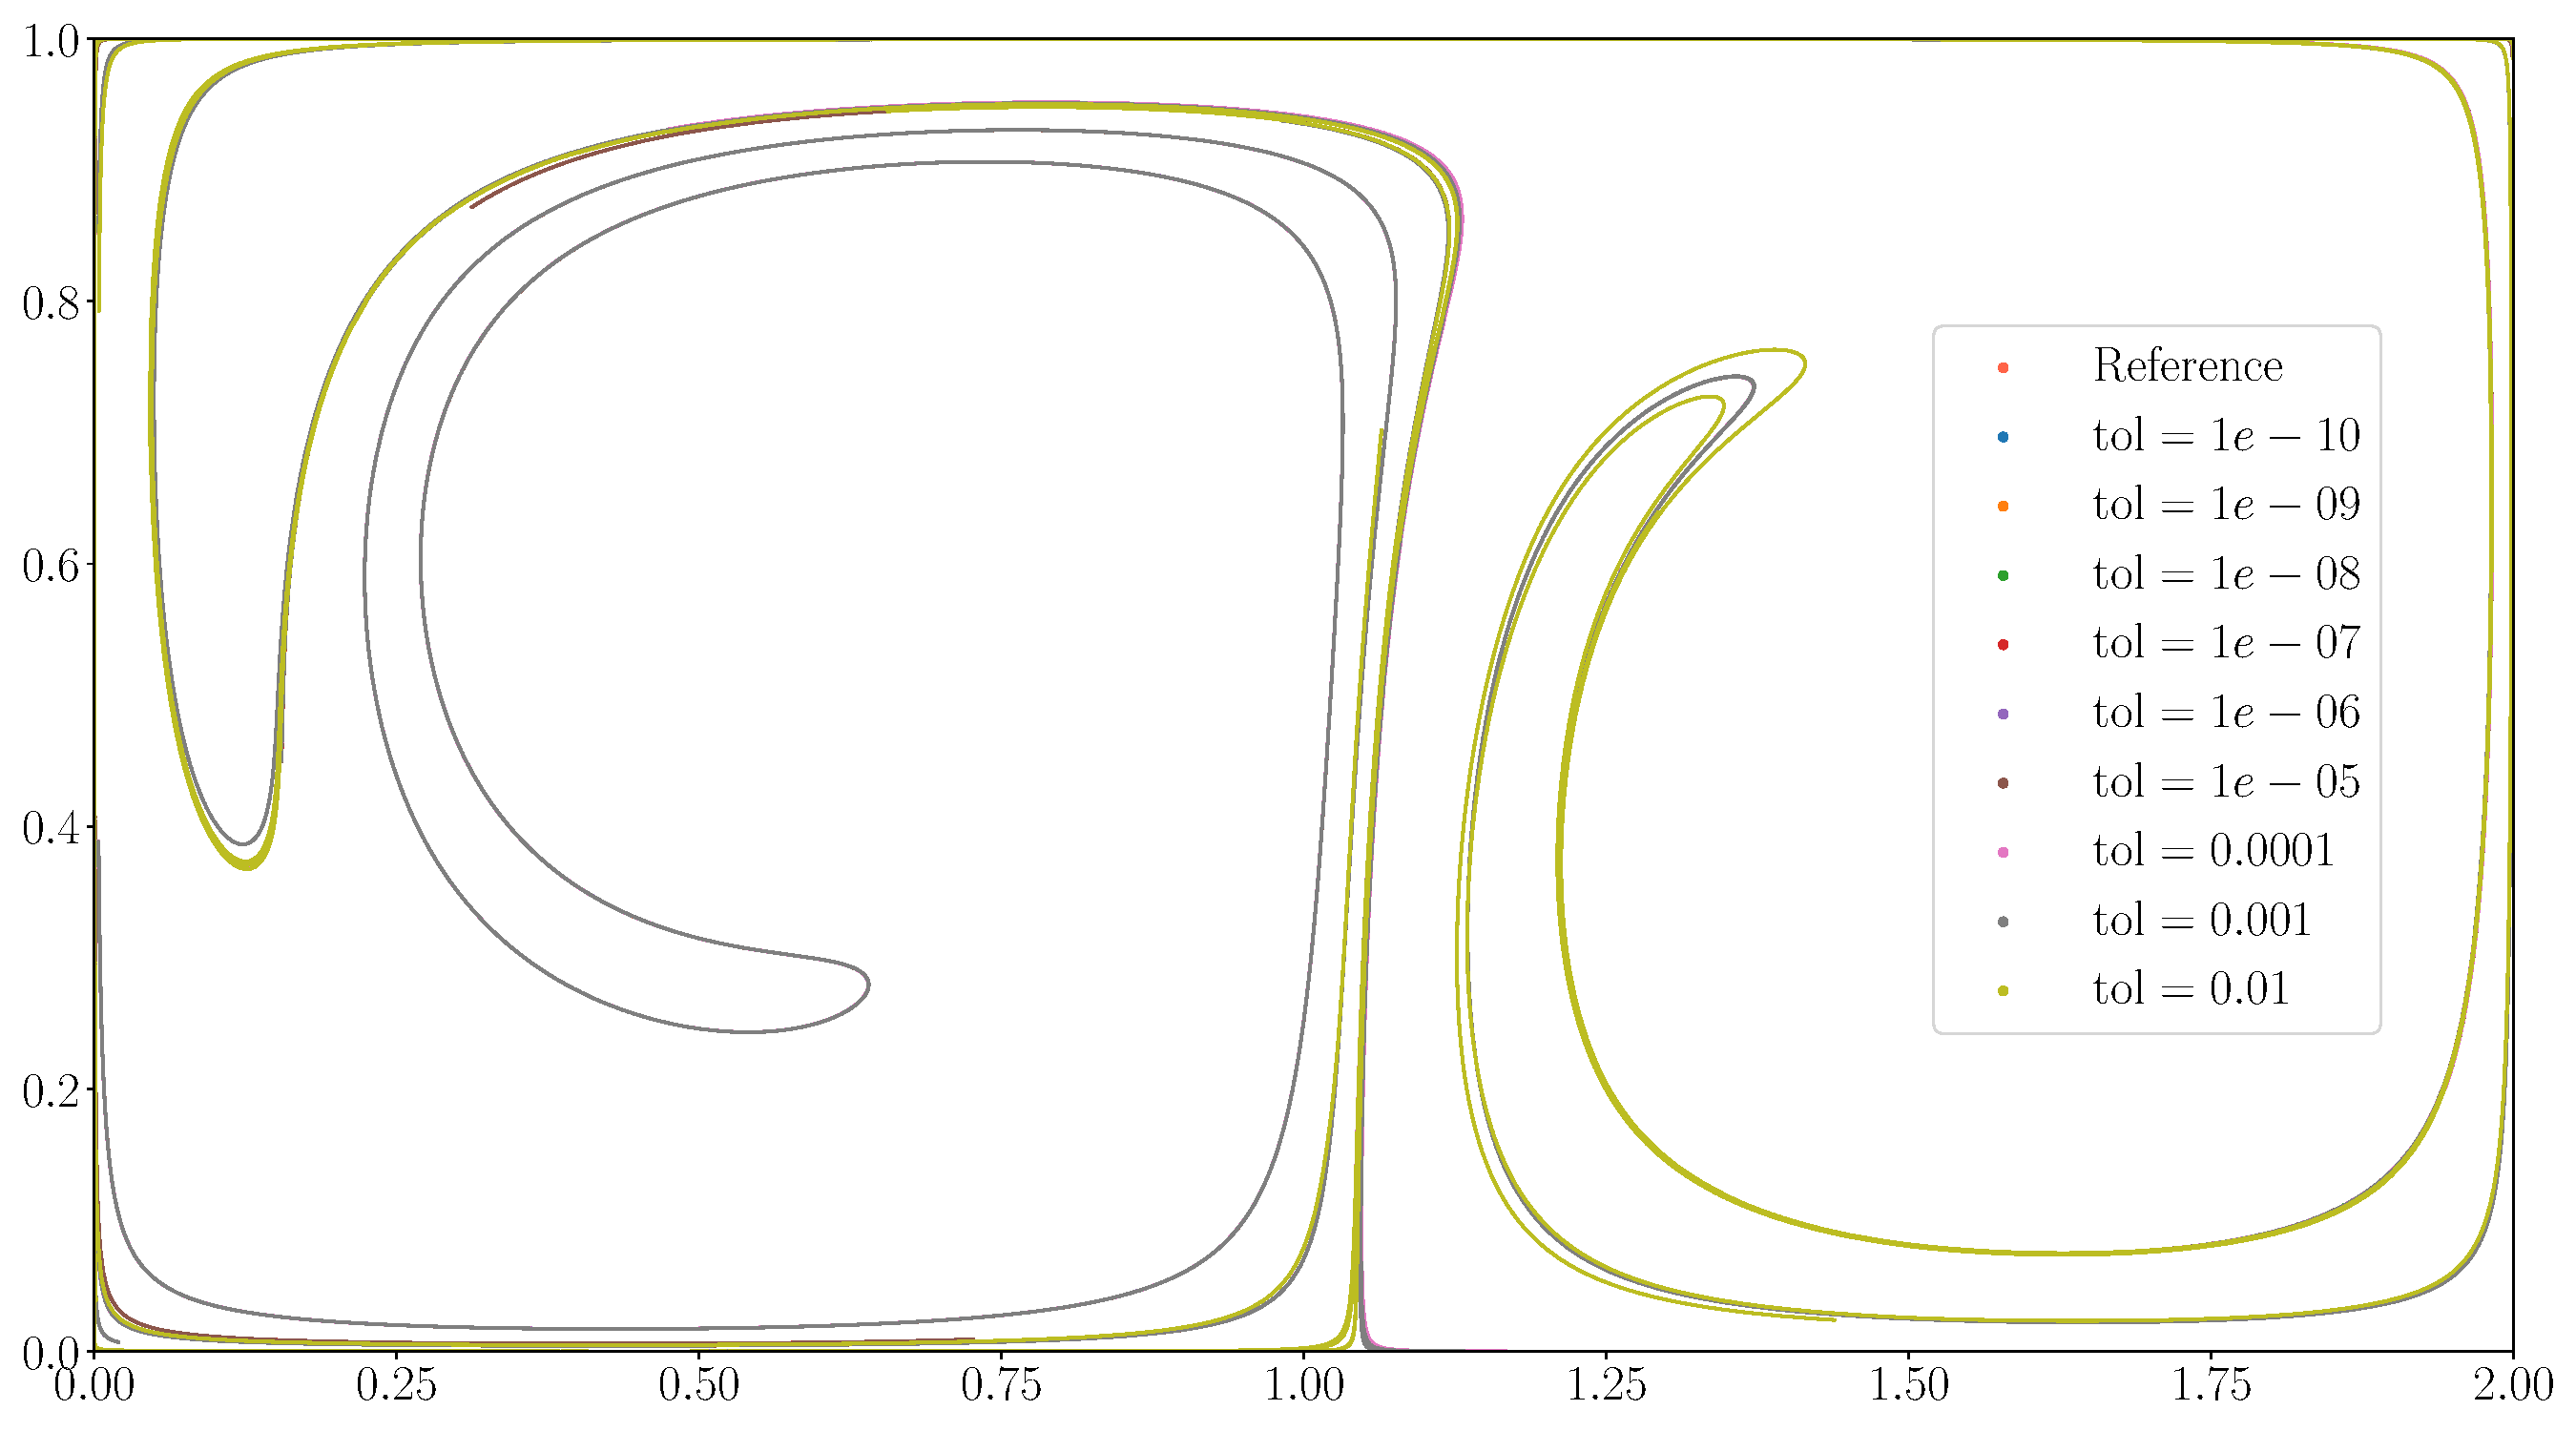
\includegraphics[width=0.9\linewidth]{figures/lcs_figures/rkdp87.pdf}
    \caption[LCS curves found by means of the Dormand-Prince 8(7) integration
    scheme]{
        LCS curves found by means of the Dormand-Prince 8(7) integration
        scheme. The reference LCS, as shown by itself in figure
        \ref{fig:referencelcs}, is dashed on the top layer. Note that
        the LCS for the lowest tolerance level considered, that is,
        $\textnormal{tol}=10^{-1}$, is not included. This is because the
        corresponding $\mathcal{U}_{0}$ domain, shown in figure
        \ref{fig:u0_dom_err_dp87}, and the reference $\mathcal{U}_{0}$, shown in figure
        \ref{fig:u0_domain} are quite unlike one another. Here, the most immediately
        discernible dissimilarities emanate from the tolerance level
    $\textnormal{tol}=10^{-2}$.}
    %Close inspection, however, reveals
    %    discrepancies for all tolerance levels $\textnormal{tol}>10^{-6}$,
    %    particularly by the `$\cap$' shape near $x=1.25$.}
    \label{fig:lcs_rkdp87}
\end{figure}
